\documentclass[twoside]{book}

% Packages required by doxygen
\usepackage{fixltx2e}
\usepackage{calc}
\usepackage{doxygen}
\usepackage[export]{adjustbox} % also loads graphicx
\usepackage{graphicx}
\usepackage[utf8]{inputenc}
\usepackage{makeidx}
\usepackage{multicol}
\usepackage{multirow}
\PassOptionsToPackage{warn}{textcomp}
\usepackage{textcomp}
\usepackage[nointegrals]{wasysym}
\usepackage[table]{xcolor}

% Font selection
\usepackage[T1]{fontenc}
\usepackage[scaled=.90]{helvet}
\usepackage{courier}
\usepackage{amssymb}
\usepackage{sectsty}
\renewcommand{\familydefault}{\sfdefault}
\allsectionsfont{%
  \fontseries{bc}\selectfont%
  \color{darkgray}%
}
\renewcommand{\DoxyLabelFont}{%
  \fontseries{bc}\selectfont%
  \color{darkgray}%
}
\newcommand{\+}{\discretionary{\mbox{\scriptsize$\hookleftarrow$}}{}{}}

% Page & text layout
\usepackage{geometry}
\geometry{%
  a4paper,%
  top=2.5cm,%
  bottom=2.5cm,%
  left=2.5cm,%
  right=2.5cm%
}
\tolerance=750
\hfuzz=15pt
\hbadness=750
\setlength{\emergencystretch}{15pt}
\setlength{\parindent}{0cm}
\setlength{\parskip}{3ex plus 2ex minus 2ex}
\makeatletter
\renewcommand{\paragraph}{%
  \@startsection{paragraph}{4}{0ex}{-1.0ex}{1.0ex}{%
    \normalfont\normalsize\bfseries\SS@parafont%
  }%
}
\renewcommand{\subparagraph}{%
  \@startsection{subparagraph}{5}{0ex}{-1.0ex}{1.0ex}{%
    \normalfont\normalsize\bfseries\SS@subparafont%
  }%
}
\makeatother

% Headers & footers
\usepackage{fancyhdr}
\pagestyle{fancyplain}
\fancyhead[LE]{\fancyplain{}{\bfseries\thepage}}
\fancyhead[CE]{\fancyplain{}{}}
\fancyhead[RE]{\fancyplain{}{\bfseries\leftmark}}
\fancyhead[LO]{\fancyplain{}{\bfseries\rightmark}}
\fancyhead[CO]{\fancyplain{}{}}
\fancyhead[RO]{\fancyplain{}{\bfseries\thepage}}
\fancyfoot[LE]{\fancyplain{}{}}
\fancyfoot[CE]{\fancyplain{}{}}
\fancyfoot[RE]{\fancyplain{}{\bfseries\scriptsize Generated by Doxygen }}
\fancyfoot[LO]{\fancyplain{}{\bfseries\scriptsize Generated by Doxygen }}
\fancyfoot[CO]{\fancyplain{}{}}
\fancyfoot[RO]{\fancyplain{}{}}
\renewcommand{\footrulewidth}{0.4pt}
\renewcommand{\chaptermark}[1]{%
  \markboth{#1}{}%
}
\renewcommand{\sectionmark}[1]{%
  \markright{\thesection\ #1}%
}

% Indices & bibliography
\usepackage{natbib}
\usepackage[titles]{tocloft}
\setcounter{tocdepth}{3}
\setcounter{secnumdepth}{5}
\makeindex

% Hyperlinks (required, but should be loaded last)
\usepackage{ifpdf}
\ifpdf
  \usepackage[pdftex,pagebackref=true]{hyperref}
\else
  \usepackage[ps2pdf,pagebackref=true]{hyperref}
\fi
\hypersetup{%
  colorlinks=true,%
  linkcolor=blue,%
  citecolor=blue,%
  unicode%
}

% Custom commands
\newcommand{\clearemptydoublepage}{%
  \newpage{\pagestyle{empty}\cleardoublepage}%
}

\usepackage{caption}
\captionsetup{labelsep=space,justification=centering,font={bf},singlelinecheck=off,skip=4pt,position=top}

%===== C O N T E N T S =====

\begin{document}

% Titlepage & ToC
\hypersetup{pageanchor=false,
             bookmarksnumbered=true,
             pdfencoding=unicode
            }
\pagenumbering{alph}
\begin{titlepage}
\vspace*{7cm}
\begin{center}%
{\Large Cool\+Board\+A\+PI }\\
\vspace*{1cm}
{\large Generated by Doxygen 1.8.14}\\
\end{center}
\end{titlepage}
\clearemptydoublepage
\pagenumbering{roman}
\tableofcontents
\clearemptydoublepage
\pagenumbering{arabic}
\hypersetup{pageanchor=true}

%--- Begin generated contents ---
\chapter{Hierarchical Index}
\section{Class Hierarchy}
This inheritance list is sorted roughly, but not completely, alphabetically\+:\begin{DoxyCompactList}
\item \contentsline{section}{Base\+External\+Sensor}{\pageref{class_base_external_sensor}}{}
\begin{DoxyCompactList}
\item \contentsline{section}{External\+Sensor$<$ T $>$}{\pageref{class_external_sensor}}{}
\item \contentsline{section}{External\+Sensor$<$ Dallas\+Temperature $>$}{\pageref{class_external_sensor_3_01_dallas_temperature_01_4}}{}
\item \contentsline{section}{External\+Sensor$<$ N\+D\+I\+R\+\_\+\+I2C $>$}{\pageref{class_external_sensor_3_01_n_d_i_r___i2_c_01_4}}{}
\end{DoxyCompactList}
\item \contentsline{section}{Cool\+Board}{\pageref{class_cool_board}}{}
\item \contentsline{section}{Cool\+Board\+Led}{\pageref{class_cool_board_led}}{}
\item \contentsline{section}{Cool\+Board\+Sensors}{\pageref{class_cool_board_sensors}}{}
\item \contentsline{section}{Cool\+File\+System}{\pageref{class_cool_file_system}}{}
\item \contentsline{section}{Cool\+M\+Q\+TT}{\pageref{class_cool_m_q_t_t}}{}
\item \contentsline{section}{Cool\+Time}{\pageref{class_cool_time}}{}
\item \contentsline{section}{External\+Sensors}{\pageref{class_external_sensors}}{}
\item \contentsline{section}{Irene3000}{\pageref{class_irene3000}}{}
\item \contentsline{section}{Jetpack}{\pageref{class_jetpack}}{}
\end{DoxyCompactList}

\chapter{Class Index}
\section{Class List}
Here are the classes, structs, unions and interfaces with brief descriptions\+:\begin{DoxyCompactList}
\item\contentsline{section}{\hyperlink{class_adafruit___a_d_s1015}{Adafruit\+\_\+\+A\+D\+S1015} }{\pageref{class_adafruit___a_d_s1015}}{}
\item\contentsline{section}{\hyperlink{class_adafruit___a_d_s1115}{Adafruit\+\_\+\+A\+D\+S1115} }{\pageref{class_adafruit___a_d_s1115}}{}
\item\contentsline{section}{\hyperlink{class_adafruit___t_c_s34725}{Adafruit\+\_\+\+T\+C\+S34725} }{\pageref{class_adafruit___t_c_s34725}}{}
\item\contentsline{section}{\hyperlink{struct_cool_board_sensors_1_1air_active}{Cool\+Board\+Sensors\+::air\+Active} }{\pageref{struct_cool_board_sensors_1_1air_active}}{}
\item\contentsline{section}{\hyperlink{class_base_external_sensor}{Base\+External\+Sensor} \\*This class is a generic external Sensor it is a way to access real external sensor methods through run Time polymorphism }{\pageref{class_base_external_sensor}}{}
\item\contentsline{section}{\hyperlink{class_b_m_e280}{B\+M\+E280} }{\pageref{class_b_m_e280}}{}
\item\contentsline{section}{\hyperlink{class_cool_board}{Cool\+Board} \\*This class manages the \hyperlink{class_cool_board}{Cool\+Board} and all of Its functions }{\pageref{class_cool_board}}{}
\item\contentsline{section}{\hyperlink{class_cool_board_actor}{Cool\+Board\+Actor} \\*This class manages the \hyperlink{class_cool_board_actor}{Cool\+Board\+Actor} }{\pageref{class_cool_board_actor}}{}
\item\contentsline{section}{\hyperlink{class_cool_board_led}{Cool\+Board\+Led} \\*This class handles the led in the Sensor Board }{\pageref{class_cool_board_led}}{}
\item\contentsline{section}{\hyperlink{class_cool_board_sensors}{Cool\+Board\+Sensors} \\*This class handles the On-\/\+Board Sensors }{\pageref{class_cool_board_sensors}}{}
\item\contentsline{section}{\hyperlink{class_cool_file_system}{Cool\+File\+System} \\*This class handles the file system }{\pageref{class_cool_file_system}}{}
\item\contentsline{section}{\hyperlink{class_cool_m_q_t_t}{Cool\+M\+Q\+TT} \\*This class handles the mqtt client }{\pageref{class_cool_m_q_t_t}}{}
\item\contentsline{section}{\hyperlink{class_cool_pub_sub_client}{Cool\+Pub\+Sub\+Client} }{\pageref{class_cool_pub_sub_client}}{}
\item\contentsline{section}{\hyperlink{class_cool_s_i114_x}{Cool\+S\+I114X} }{\pageref{class_cool_s_i114_x}}{}
\item\contentsline{section}{\hyperlink{class_cool_time}{Cool\+Time} \\*This class manages the D\+S1337 R\+TC }{\pageref{class_cool_time}}{}
\item\contentsline{section}{\hyperlink{class_cool_wifi}{Cool\+Wifi} \\*This class manages the Wi\+Fi connection }{\pageref{class_cool_wifi}}{}
\item\contentsline{section}{\hyperlink{class_external_sensor}{External\+Sensor$<$ T $>$} \\*Template$<$class Sensor\+Class$>$ class External Sensor\+: Derived class from \hyperlink{class_base_external_sensor}{Base\+External\+Sensor} }{\pageref{class_external_sensor}}{}
\item\contentsline{section}{\hyperlink{class_external_sensor_3_01_adafruit___a_d_s1015_01_4}{External\+Sensor$<$ Adafruit\+\_\+\+A\+D\+S1015 $>$} \\*\hyperlink{class_adafruit___a_d_s1015}{Adafruit\+\_\+\+A\+D\+S1015} Specialization Class This is the template specialization for the Adafruit Analog I2C Interface }{\pageref{class_external_sensor_3_01_adafruit___a_d_s1015_01_4}}{}
\item\contentsline{section}{\hyperlink{class_external_sensor_3_01_adafruit___a_d_s1115_01_4}{External\+Sensor$<$ Adafruit\+\_\+\+A\+D\+S1115 $>$} \\*\hyperlink{class_adafruit___a_d_s1115}{Adafruit\+\_\+\+A\+D\+S1115} Specialization Class This is the template specialization for the Adafruit Analog I2C Interface }{\pageref{class_external_sensor_3_01_adafruit___a_d_s1115_01_4}}{}
\item\contentsline{section}{\hyperlink{class_external_sensor_3_01_adafruit___t_c_s34725_01_4}{External\+Sensor$<$ Adafruit\+\_\+\+T\+C\+S34725 $>$} \\*\hyperlink{class_adafruit___t_c_s34725}{Adafruit\+\_\+\+T\+C\+S34725} Specialization Class This is the template specialization for the Adafruit R\+GB Sensor }{\pageref{class_external_sensor_3_01_adafruit___t_c_s34725_01_4}}{}
\item\contentsline{section}{\hyperlink{class_external_sensor_3_01_dallas_temperature_01_4}{External\+Sensor$<$ Dallas\+Temperature $>$} \\*Dallas\+Temperature Specialization Class This is the template specialization for the Dallas Temperature sensor }{\pageref{class_external_sensor_3_01_dallas_temperature_01_4}}{}
\item\contentsline{section}{\hyperlink{class_external_sensor_3_01_n_d_i_r___i2_c_01_4}{External\+Sensor$<$ N\+D\+I\+R\+\_\+\+I2\+C $>$} \\*\hyperlink{class_n_d_i_r___i2_c}{N\+D\+I\+R\+\_\+\+I2C} Specialization Class This is the template specialization for the \hyperlink{class_n_d_i_r___i2_c}{N\+D\+I\+R\+\_\+\+I2C} C\+O2 sensor }{\pageref{class_external_sensor_3_01_n_d_i_r___i2_c_01_4}}{}
\item\contentsline{section}{\hyperlink{class_external_sensors}{External\+Sensors} \\*This class handles the external sensors run time defintion , configuartion and actions }{\pageref{class_external_sensors}}{}
\item\contentsline{section}{\hyperlink{class_irene3000}{Irene3000} \\*This class is provided to manage the \hyperlink{class_irene3000}{Irene3000} Ph/\+Temperature Shield }{\pageref{class_irene3000}}{}
\item\contentsline{section}{\hyperlink{class_jetpack}{Jetpack} \\*This class manages the \hyperlink{class_jetpack}{Jetpack} shield }{\pageref{class_jetpack}}{}
\item\contentsline{section}{\hyperlink{struct_cool_board_sensors_1_1light_active}{Cool\+Board\+Sensors\+::light\+Active} }{\pageref{struct_cool_board_sensors_1_1light_active}}{}
\item\contentsline{section}{\hyperlink{class_n_d_i_r___i2_c}{N\+D\+I\+R\+\_\+\+I2C} }{\pageref{class_n_d_i_r___i2_c}}{}
\item\contentsline{section}{\hyperlink{struct_irene3000_1_1parameters___t}{Irene3000\+::parameters\+\_\+T} }{\pageref{struct_irene3000_1_1parameters___t}}{}
\item\contentsline{section}{\hyperlink{struct_external_sensors_1_1sensor}{External\+Sensors\+::sensor} }{\pageref{struct_external_sensors_1_1sensor}}{}
\item\contentsline{section}{\hyperlink{struct_sensor_calibration}{Sensor\+Calibration} }{\pageref{struct_sensor_calibration}}{}
\item\contentsline{section}{\hyperlink{struct_sensor_settings}{Sensor\+Settings} }{\pageref{struct_sensor_settings}}{}
\item\contentsline{section}{\hyperlink{struct_cool_board_actor_1_1state}{Cool\+Board\+Actor\+::state} }{\pageref{struct_cool_board_actor_1_1state}}{}
\item\contentsline{section}{\hyperlink{struct_irene3000_1_1state}{Irene3000\+::state} }{\pageref{struct_irene3000_1_1state}}{}
\item\contentsline{section}{\hyperlink{struct_jetpack_1_1state}{Jetpack\+::state} }{\pageref{struct_jetpack_1_1state}}{}
\item\contentsline{section}{\hyperlink{class_wi_fi_manager}{Wi\+Fi\+Manager} }{\pageref{class_wi_fi_manager}}{}
\item\contentsline{section}{\hyperlink{class_wi_fi_manager_parameter}{Wi\+Fi\+Manager\+Parameter} }{\pageref{class_wi_fi_manager_parameter}}{}
\end{DoxyCompactList}

\chapter{File Index}
\section{File List}
Here is a list of all files with brief descriptions\+:\begin{DoxyCompactList}
\item\contentsline{section}{/home/ashiroji/\+Arduino/libraries/\+Cool\+Board/src/\hyperlink{_cool_board_8cpp}{Cool\+Board.\+cpp} \\*\hyperlink{class_cool_board}{Cool\+Board} Source file }{\pageref{_cool_board_8cpp}}{}
\item\contentsline{section}{/home/ashiroji/\+Arduino/libraries/\+Cool\+Board/src/\hyperlink{_cool_board_8h}{Cool\+Board.\+h} \\*\hyperlink{class_cool_board}{Cool\+Board} Header file }{\pageref{_cool_board_8h}}{}
\item\contentsline{section}{/home/ashiroji/\+Arduino/libraries/\+Cool\+Board/src/\hyperlink{_cool_board_actor_8cpp}{Cool\+Board\+Actor.\+cpp} \\*\hyperlink{class_cool_board_actor}{Cool\+Board\+Actor} Source File }{\pageref{_cool_board_actor_8cpp}}{}
\item\contentsline{section}{/home/ashiroji/\+Arduino/libraries/\+Cool\+Board/src/\hyperlink{_cool_board_actor_8h}{Cool\+Board\+Actor.\+h} \\*\hyperlink{class_cool_board_actor}{Cool\+Board\+Actor} Header File }{\pageref{_cool_board_actor_8h}}{}
\item\contentsline{section}{/home/ashiroji/\+Arduino/libraries/\+Cool\+Board/src/\hyperlink{_cool_board_led_8cpp}{Cool\+Board\+Led.\+cpp} \\*\hyperlink{class_cool_board_led}{Cool\+Board\+Led} Source File }{\pageref{_cool_board_led_8cpp}}{}
\item\contentsline{section}{/home/ashiroji/\+Arduino/libraries/\+Cool\+Board/src/\hyperlink{_cool_board_led_8h}{Cool\+Board\+Led.\+h} \\*\hyperlink{class_cool_board_led}{Cool\+Board\+Led} Header File }{\pageref{_cool_board_led_8h}}{}
\item\contentsline{section}{/home/ashiroji/\+Arduino/libraries/\+Cool\+Board/src/\hyperlink{_cool_board_sensors_8cpp}{Cool\+Board\+Sensors.\+cpp} \\*\hyperlink{class_cool_board_sensors}{Cool\+Board\+Sensors} Source File }{\pageref{_cool_board_sensors_8cpp}}{}
\item\contentsline{section}{/home/ashiroji/\+Arduino/libraries/\+Cool\+Board/src/\hyperlink{_cool_board_sensors_8h}{Cool\+Board\+Sensors.\+h} \\*\hyperlink{class_cool_board_sensors}{Cool\+Board\+Sensors} Header File }{\pageref{_cool_board_sensors_8h}}{}
\item\contentsline{section}{/home/ashiroji/\+Arduino/libraries/\+Cool\+Board/src/\hyperlink{_cool_file_system_8cpp}{Cool\+File\+System.\+cpp} \\*\hyperlink{class_cool_file_system}{Cool\+File\+System} Source File }{\pageref{_cool_file_system_8cpp}}{}
\item\contentsline{section}{/home/ashiroji/\+Arduino/libraries/\+Cool\+Board/src/\hyperlink{_cool_file_system_8h}{Cool\+File\+System.\+h} \\*\hyperlink{class_cool_file_system}{Cool\+File\+System} Header File }{\pageref{_cool_file_system_8h}}{}
\item\contentsline{section}{/home/ashiroji/\+Arduino/libraries/\+Cool\+Board/src/\hyperlink{_cool_m_q_t_t_8cpp}{Cool\+M\+Q\+T\+T.\+cpp} \\*\hyperlink{class_cool_m_q_t_t}{Cool\+M\+Q\+TT} Source File }{\pageref{_cool_m_q_t_t_8cpp}}{}
\item\contentsline{section}{/home/ashiroji/\+Arduino/libraries/\+Cool\+Board/src/\hyperlink{_cool_m_q_t_t_8h}{Cool\+M\+Q\+T\+T.\+h} \\*\hyperlink{class_cool_m_q_t_t}{Cool\+M\+Q\+TT} Header File }{\pageref{_cool_m_q_t_t_8h}}{}
\item\contentsline{section}{/home/ashiroji/\+Arduino/libraries/\+Cool\+Board/src/\hyperlink{_cool_time_8cpp}{Cool\+Time.\+cpp} \\*\hyperlink{class_cool_time}{Cool\+Time} Source File }{\pageref{_cool_time_8cpp}}{}
\item\contentsline{section}{/home/ashiroji/\+Arduino/libraries/\+Cool\+Board/src/\hyperlink{_cool_time_8h}{Cool\+Time.\+h} \\*\hyperlink{class_cool_time}{Cool\+Time} Header File }{\pageref{_cool_time_8h}}{}
\item\contentsline{section}{/home/ashiroji/\+Arduino/libraries/\+Cool\+Board/src/\hyperlink{_cool_wifi_8cpp}{Cool\+Wifi.\+cpp} \\*\hyperlink{class_cool_wifi}{Cool\+Wifi} Source File }{\pageref{_cool_wifi_8cpp}}{}
\item\contentsline{section}{/home/ashiroji/\+Arduino/libraries/\+Cool\+Board/src/\hyperlink{_cool_wifi_8h}{Cool\+Wifi.\+h} \\*\hyperlink{class_cool_wifi}{Cool\+Wifi} Header File }{\pageref{_cool_wifi_8h}}{}
\item\contentsline{section}{/home/ashiroji/\+Arduino/libraries/\+Cool\+Board/src/\hyperlink{_external_sensor_8h}{External\+Sensor.\+h} \\*\hyperlink{class_external_sensor}{External\+Sensor} Header File }{\pageref{_external_sensor_8h}}{}
\item\contentsline{section}{/home/ashiroji/\+Arduino/libraries/\+Cool\+Board/src/\hyperlink{_external_sensors_8cpp}{External\+Sensors.\+cpp} \\*\hyperlink{class_external_sensors}{External\+Sensors} Source File }{\pageref{_external_sensors_8cpp}}{}
\item\contentsline{section}{/home/ashiroji/\+Arduino/libraries/\+Cool\+Board/src/\hyperlink{_external_sensors_8h}{External\+Sensors.\+h} \\*\hyperlink{class_external_sensors}{External\+Sensors} Header File }{\pageref{_external_sensors_8h}}{}
\item\contentsline{section}{/home/ashiroji/\+Arduino/libraries/\+Cool\+Board/src/\hyperlink{irene3000_8cpp}{irene3000.\+cpp} \\*\hyperlink{class_irene3000}{Irene3000} Source File }{\pageref{irene3000_8cpp}}{}
\item\contentsline{section}{/home/ashiroji/\+Arduino/libraries/\+Cool\+Board/src/\hyperlink{_irene3000_8h}{Irene3000.\+h} \\*\hyperlink{class_irene3000}{Irene3000} Header File }{\pageref{_irene3000_8h}}{}
\item\contentsline{section}{/home/ashiroji/\+Arduino/libraries/\+Cool\+Board/src/\hyperlink{_jetpack_8cpp}{Jetpack.\+cpp} \\*\hyperlink{class_jetpack}{Jetpack} Source File }{\pageref{_jetpack_8cpp}}{}
\item\contentsline{section}{/home/ashiroji/\+Arduino/libraries/\+Cool\+Board/src/\hyperlink{_jetpack_8h}{Jetpack.\+h} \\*\hyperlink{class_jetpack}{Jetpack} Header File }{\pageref{_jetpack_8h}}{}
\item\contentsline{section}{/home/ashiroji/\+Arduino/libraries/\+Cool\+Board/src/internals/\hyperlink{_cool_adafruit___a_d_s1015_8cpp}{Cool\+Adafruit\+\_\+\+A\+D\+S1015.\+cpp} }{\pageref{_cool_adafruit___a_d_s1015_8cpp}}{}
\item\contentsline{section}{/home/ashiroji/\+Arduino/libraries/\+Cool\+Board/src/internals/\hyperlink{_cool_adafruit___a_d_s1015_8h}{Cool\+Adafruit\+\_\+\+A\+D\+S1015.\+h} }{\pageref{_cool_adafruit___a_d_s1015_8h}}{}
\item\contentsline{section}{/home/ashiroji/\+Arduino/libraries/\+Cool\+Board/src/internals/\hyperlink{_cool_n_d_i_r___i2_c_8cpp}{Cool\+N\+D\+I\+R\+\_\+\+I2\+C.\+cpp} }{\pageref{_cool_n_d_i_r___i2_c_8cpp}}{}
\item\contentsline{section}{/home/ashiroji/\+Arduino/libraries/\+Cool\+Board/src/internals/\hyperlink{_cool_n_d_i_r___i2_c_8h}{Cool\+N\+D\+I\+R\+\_\+\+I2\+C.\+h} }{\pageref{_cool_n_d_i_r___i2_c_8h}}{}
\item\contentsline{section}{/home/ashiroji/\+Arduino/libraries/\+Cool\+Board/src/internals/\hyperlink{_cool_pub_sub_client_8cpp}{Cool\+Pub\+Sub\+Client.\+cpp} }{\pageref{_cool_pub_sub_client_8cpp}}{}
\item\contentsline{section}{/home/ashiroji/\+Arduino/libraries/\+Cool\+Board/src/internals/\hyperlink{_cool_pub_sub_client_8h}{Cool\+Pub\+Sub\+Client.\+h} }{\pageref{_cool_pub_sub_client_8h}}{}
\item\contentsline{section}{/home/ashiroji/\+Arduino/libraries/\+Cool\+Board/src/internals/\hyperlink{_cool_s_i114_x_8cpp}{Cool\+S\+I114\+X.\+cpp} }{\pageref{_cool_s_i114_x_8cpp}}{}
\item\contentsline{section}{/home/ashiroji/\+Arduino/libraries/\+Cool\+Board/src/internals/\hyperlink{_cool_s_i114_x_8h}{Cool\+S\+I114\+X.\+h} }{\pageref{_cool_s_i114_x_8h}}{}
\item\contentsline{section}{/home/ashiroji/\+Arduino/libraries/\+Cool\+Board/src/internals/\hyperlink{_cool_spark_fun_b_m_e280_8cpp}{Cool\+Spark\+Fun\+B\+M\+E280.\+cpp} }{\pageref{_cool_spark_fun_b_m_e280_8cpp}}{}
\item\contentsline{section}{/home/ashiroji/\+Arduino/libraries/\+Cool\+Board/src/internals/\hyperlink{_cool_spark_fun_b_m_e280_8h}{Cool\+Spark\+Fun\+B\+M\+E280.\+h} }{\pageref{_cool_spark_fun_b_m_e280_8h}}{}
\item\contentsline{section}{/home/ashiroji/\+Arduino/libraries/\+Cool\+Board/src/internals/\hyperlink{_wi_fi_manager_read_file_button_8cpp}{Wi\+Fi\+Manager\+Read\+File\+Button.\+cpp} }{\pageref{_wi_fi_manager_read_file_button_8cpp}}{}
\item\contentsline{section}{/home/ashiroji/\+Arduino/libraries/\+Cool\+Board/src/internals/\hyperlink{_wi_fi_manager_read_file_button_8h}{Wi\+Fi\+Manager\+Read\+File\+Button.\+h} }{\pageref{_wi_fi_manager_read_file_button_8h}}{}
\item\contentsline{section}{/home/ashiroji/\+Arduino/libraries/\+Cool\+Board/src/internals/extras/\hyperlink{parse_8js}{parse.\+js} }{\pageref{parse_8js}}{}
\item\contentsline{section}{/home/ashiroji/\+Arduino/libraries/\+Cool\+Board/src/internals/extras/\hyperlink{template_8h}{template.\+h} }{\pageref{template_8h}}{}
\end{DoxyCompactList}

\chapter{Class Documentation}
\hypertarget{class_adafruit___a_d_s1015}{}\section{Adafruit\+\_\+\+A\+D\+S1015 Class Reference}
\label{class_adafruit___a_d_s1015}\index{Adafruit\+\_\+\+A\+D\+S1015@{Adafruit\+\_\+\+A\+D\+S1015}}


{\ttfamily \#include $<$Cool\+Adafruit\+\_\+\+A\+D\+S1015.\+h$>$}



Inheritance diagram for Adafruit\+\_\+\+A\+D\+S1015\+:\nopagebreak
\begin{figure}[H]
\begin{center}
\leavevmode
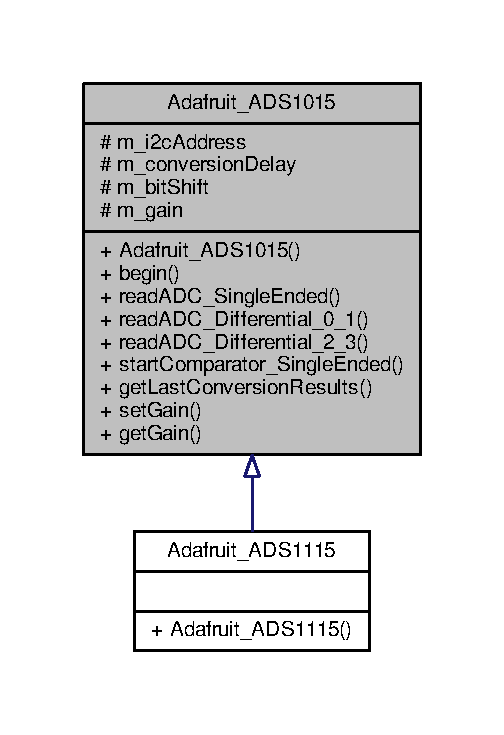
\includegraphics[width=242pt]{class_adafruit___a_d_s1015__inherit__graph}
\end{center}
\end{figure}


Collaboration diagram for Adafruit\+\_\+\+A\+D\+S1015\+:\nopagebreak
\begin{figure}[H]
\begin{center}
\leavevmode
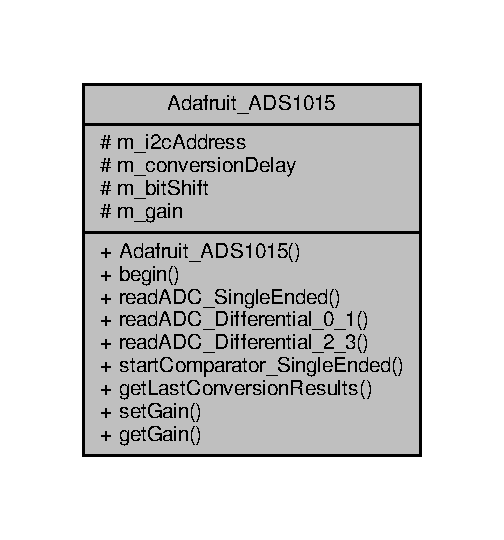
\includegraphics[width=242pt]{class_adafruit___a_d_s1015__coll__graph}
\end{center}
\end{figure}
\subsection*{Public Member Functions}
\begin{DoxyCompactItemize}
\item 
\hyperlink{class_adafruit___a_d_s1015_a12dfb7b48af1a8e411c59f775c6457ab}{Adafruit\+\_\+\+A\+D\+S1015} (uint8\+\_\+t i2c\+Address=\hyperlink{_cool_adafruit___a_d_s1015_8h_ae55d158023984e8f0ddc80b58d5b30dc}{A\+D\+S1015\+\_\+\+A\+D\+D\+R\+E\+SS})
\begin{DoxyCompactList}\small\item\em Instantiates a new A\+D\+S1015 class w/appropriate properties. \end{DoxyCompactList}\item 
void \hyperlink{class_adafruit___a_d_s1015_a6eba7c3cd854927f60883bb371e5faa6}{begin} (void)
\begin{DoxyCompactList}\small\item\em Sets up the HW (reads coefficients values, etc.) \end{DoxyCompactList}\item 
uint16\+\_\+t \hyperlink{class_adafruit___a_d_s1015_a40f38b9e1f3ec397c0670dd632510235}{read\+A\+D\+C\+\_\+\+Single\+Ended} (uint8\+\_\+t channel)
\begin{DoxyCompactList}\small\item\em Gets a single-\/ended A\+DC reading from the specified channel. \end{DoxyCompactList}\item 
int16\+\_\+t \hyperlink{class_adafruit___a_d_s1015_a56582333958e66efaccd3d4a8a47e3ff}{read\+A\+D\+C\+\_\+\+Differential\+\_\+0\+\_\+1} (void)
\begin{DoxyCompactList}\small\item\em Reads the conversion results, measuring the voltage difference between the P (A\+I\+N0) and N (A\+I\+N1) input. Generates a signed value since the difference can be either positive or negative. \end{DoxyCompactList}\item 
int16\+\_\+t \hyperlink{class_adafruit___a_d_s1015_a38311881bcab46f7496c4bb6e4cad576}{read\+A\+D\+C\+\_\+\+Differential\+\_\+2\+\_\+3} (void)
\begin{DoxyCompactList}\small\item\em Reads the conversion results, measuring the voltage difference between the P (A\+I\+N2) and N (A\+I\+N3) input. Generates a signed value since the difference can be either positive or negative. \end{DoxyCompactList}\item 
void \hyperlink{class_adafruit___a_d_s1015_aecd30775d943ea9d9cff0e3485926596}{start\+Comparator\+\_\+\+Single\+Ended} (uint8\+\_\+t channel, int16\+\_\+t threshold)
\begin{DoxyCompactList}\small\item\em Sets up the comparator to operate in basic mode, causing the A\+L\+E\+R\+T/\+R\+DY pin to assert (go from high to low) when the A\+DC value exceeds the specified threshold. \end{DoxyCompactList}\item 
int16\+\_\+t \hyperlink{class_adafruit___a_d_s1015_ad8f36d80847020778425107f6451a8c2}{get\+Last\+Conversion\+Results} ()
\begin{DoxyCompactList}\small\item\em In order to clear the comparator, we need to read the conversion results. This function reads the last conversion results without changing the config value. \end{DoxyCompactList}\item 
void \hyperlink{class_adafruit___a_d_s1015_a399441eace686975ff22937cbe45cc50}{set\+Gain} (\hyperlink{_cool_adafruit___a_d_s1015_8h_a3d6c0e15829a207b9155890811fa4781}{ads\+Gain\+\_\+t} gain)
\begin{DoxyCompactList}\small\item\em Sets the gain and input voltage range. \end{DoxyCompactList}\item 
\hyperlink{_cool_adafruit___a_d_s1015_8h_a3d6c0e15829a207b9155890811fa4781}{ads\+Gain\+\_\+t} \hyperlink{class_adafruit___a_d_s1015_a6232d089aaa82226bc34623fdf92237c}{get\+Gain} (void)
\begin{DoxyCompactList}\small\item\em Gets a gain and input voltage range. \end{DoxyCompactList}\end{DoxyCompactItemize}
\subsection*{Protected Attributes}
\begin{DoxyCompactItemize}
\item 
uint8\+\_\+t \hyperlink{class_adafruit___a_d_s1015_a2186993621a7973256d47f086c74035d}{m\+\_\+i2c\+Address}
\item 
uint8\+\_\+t \hyperlink{class_adafruit___a_d_s1015_aa3a29a64a6705fce1fee21d73c642a0e}{m\+\_\+conversion\+Delay}
\item 
uint8\+\_\+t \hyperlink{class_adafruit___a_d_s1015_ab238ce17112a78db2be4ea14d57fb114}{m\+\_\+bit\+Shift}
\item 
\hyperlink{_cool_adafruit___a_d_s1015_8h_a3d6c0e15829a207b9155890811fa4781}{ads\+Gain\+\_\+t} \hyperlink{class_adafruit___a_d_s1015_a8db90fe03d55a18246984ba2ba5e7f32}{m\+\_\+gain}
\end{DoxyCompactItemize}


\subsection{Detailed Description}


Definition at line 119 of file Cool\+Adafruit\+\_\+\+A\+D\+S1015.\+h.



\subsection{Constructor \& Destructor Documentation}
\mbox{\Hypertarget{class_adafruit___a_d_s1015_a12dfb7b48af1a8e411c59f775c6457ab}\label{class_adafruit___a_d_s1015_a12dfb7b48af1a8e411c59f775c6457ab}} 
\index{Adafruit\+\_\+\+A\+D\+S1015@{Adafruit\+\_\+\+A\+D\+S1015}!Adafruit\+\_\+\+A\+D\+S1015@{Adafruit\+\_\+\+A\+D\+S1015}}
\index{Adafruit\+\_\+\+A\+D\+S1015@{Adafruit\+\_\+\+A\+D\+S1015}!Adafruit\+\_\+\+A\+D\+S1015@{Adafruit\+\_\+\+A\+D\+S1015}}
\subsubsection{\texorpdfstring{Adafruit\+\_\+\+A\+D\+S1015()}{Adafruit\_ADS1015()}}
{\footnotesize\ttfamily Adafruit\+\_\+\+A\+D\+S1015\+::\+Adafruit\+\_\+\+A\+D\+S1015 (\begin{DoxyParamCaption}\item[{uint8\+\_\+t}]{i2c\+Address = {\ttfamily \hyperlink{_cool_adafruit___a_d_s1015_8h_ae55d158023984e8f0ddc80b58d5b30dc}{A\+D\+S1015\+\_\+\+A\+D\+D\+R\+E\+SS}} }\end{DoxyParamCaption})}



Instantiates a new A\+D\+S1015 class w/appropriate properties. 



Definition at line 88 of file Cool\+Adafruit\+\_\+\+A\+D\+S1015.\+cpp.



\subsection{Member Function Documentation}
\mbox{\Hypertarget{class_adafruit___a_d_s1015_a6eba7c3cd854927f60883bb371e5faa6}\label{class_adafruit___a_d_s1015_a6eba7c3cd854927f60883bb371e5faa6}} 
\index{Adafruit\+\_\+\+A\+D\+S1015@{Adafruit\+\_\+\+A\+D\+S1015}!begin@{begin}}
\index{begin@{begin}!Adafruit\+\_\+\+A\+D\+S1015@{Adafruit\+\_\+\+A\+D\+S1015}}
\subsubsection{\texorpdfstring{begin()}{begin()}}
{\footnotesize\ttfamily void Adafruit\+\_\+\+A\+D\+S1015\+::begin (\begin{DoxyParamCaption}\item[{void}]{ }\end{DoxyParamCaption})}



Sets up the HW (reads coefficients values, etc.) 



Definition at line 114 of file Cool\+Adafruit\+\_\+\+A\+D\+S1015.\+cpp.

Here is the caller graph for this function\+:\nopagebreak
\begin{figure}[H]
\begin{center}
\leavevmode
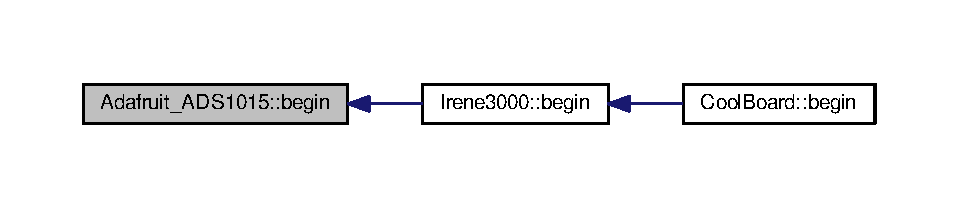
\includegraphics[width=350pt]{class_adafruit___a_d_s1015_a6eba7c3cd854927f60883bb371e5faa6_icgraph}
\end{center}
\end{figure}
\mbox{\Hypertarget{class_adafruit___a_d_s1015_a6232d089aaa82226bc34623fdf92237c}\label{class_adafruit___a_d_s1015_a6232d089aaa82226bc34623fdf92237c}} 
\index{Adafruit\+\_\+\+A\+D\+S1015@{Adafruit\+\_\+\+A\+D\+S1015}!get\+Gain@{get\+Gain}}
\index{get\+Gain@{get\+Gain}!Adafruit\+\_\+\+A\+D\+S1015@{Adafruit\+\_\+\+A\+D\+S1015}}
\subsubsection{\texorpdfstring{get\+Gain()}{getGain()}}
{\footnotesize\ttfamily \hyperlink{_cool_adafruit___a_d_s1015_8h_a3d6c0e15829a207b9155890811fa4781}{ads\+Gain\+\_\+t} Adafruit\+\_\+\+A\+D\+S1015\+::get\+Gain (\begin{DoxyParamCaption}\item[{void}]{ }\end{DoxyParamCaption})}



Gets a gain and input voltage range. 



Definition at line 133 of file Cool\+Adafruit\+\_\+\+A\+D\+S1015.\+cpp.

\mbox{\Hypertarget{class_adafruit___a_d_s1015_ad8f36d80847020778425107f6451a8c2}\label{class_adafruit___a_d_s1015_ad8f36d80847020778425107f6451a8c2}} 
\index{Adafruit\+\_\+\+A\+D\+S1015@{Adafruit\+\_\+\+A\+D\+S1015}!get\+Last\+Conversion\+Results@{get\+Last\+Conversion\+Results}}
\index{get\+Last\+Conversion\+Results@{get\+Last\+Conversion\+Results}!Adafruit\+\_\+\+A\+D\+S1015@{Adafruit\+\_\+\+A\+D\+S1015}}
\subsubsection{\texorpdfstring{get\+Last\+Conversion\+Results()}{getLastConversionResults()}}
{\footnotesize\ttfamily int16\+\_\+t Adafruit\+\_\+\+A\+D\+S1015\+::get\+Last\+Conversion\+Results (\begin{DoxyParamCaption}{ }\end{DoxyParamCaption})}



In order to clear the comparator, we need to read the conversion results. This function reads the last conversion results without changing the config value. 



Definition at line 348 of file Cool\+Adafruit\+\_\+\+A\+D\+S1015.\+cpp.

Here is the call graph for this function\+:\nopagebreak
\begin{figure}[H]
\begin{center}
\leavevmode
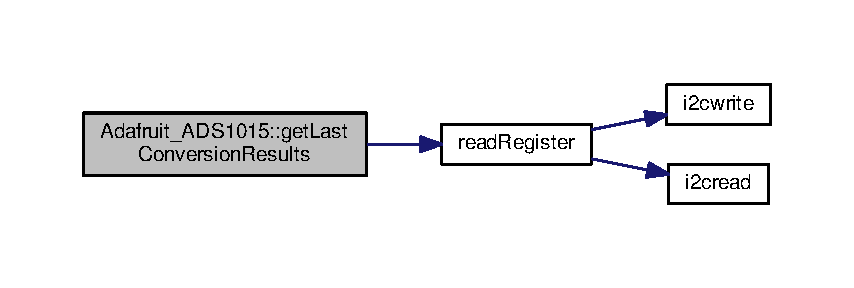
\includegraphics[width=350pt]{class_adafruit___a_d_s1015_ad8f36d80847020778425107f6451a8c2_cgraph}
\end{center}
\end{figure}
\mbox{\Hypertarget{class_adafruit___a_d_s1015_a56582333958e66efaccd3d4a8a47e3ff}\label{class_adafruit___a_d_s1015_a56582333958e66efaccd3d4a8a47e3ff}} 
\index{Adafruit\+\_\+\+A\+D\+S1015@{Adafruit\+\_\+\+A\+D\+S1015}!read\+A\+D\+C\+\_\+\+Differential\+\_\+0\+\_\+1@{read\+A\+D\+C\+\_\+\+Differential\+\_\+0\+\_\+1}}
\index{read\+A\+D\+C\+\_\+\+Differential\+\_\+0\+\_\+1@{read\+A\+D\+C\+\_\+\+Differential\+\_\+0\+\_\+1}!Adafruit\+\_\+\+A\+D\+S1015@{Adafruit\+\_\+\+A\+D\+S1015}}
\subsubsection{\texorpdfstring{read\+A\+D\+C\+\_\+\+Differential\+\_\+0\+\_\+1()}{readADC\_Differential\_0\_1()}}
{\footnotesize\ttfamily int16\+\_\+t Adafruit\+\_\+\+A\+D\+S1015\+::read\+A\+D\+C\+\_\+\+Differential\+\_\+0\+\_\+1 (\begin{DoxyParamCaption}\item[{void}]{ }\end{DoxyParamCaption})}



Reads the conversion results, measuring the voltage difference between the P (A\+I\+N0) and N (A\+I\+N1) input. Generates a signed value since the difference can be either positive or negative. 



Definition at line 199 of file Cool\+Adafruit\+\_\+\+A\+D\+S1015.\+cpp.

Here is the call graph for this function\+:\nopagebreak
\begin{figure}[H]
\begin{center}
\leavevmode
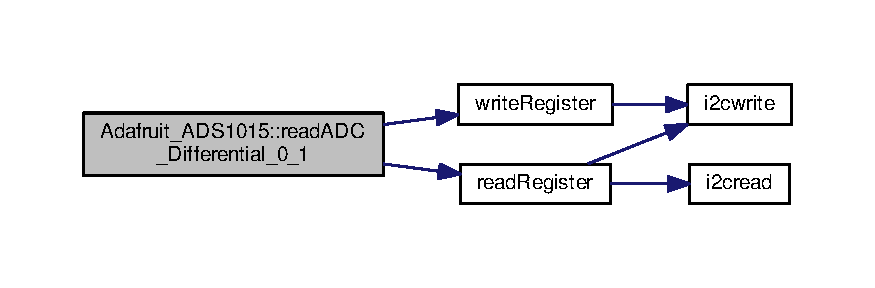
\includegraphics[width=350pt]{class_adafruit___a_d_s1015_a56582333958e66efaccd3d4a8a47e3ff_cgraph}
\end{center}
\end{figure}
\mbox{\Hypertarget{class_adafruit___a_d_s1015_a38311881bcab46f7496c4bb6e4cad576}\label{class_adafruit___a_d_s1015_a38311881bcab46f7496c4bb6e4cad576}} 
\index{Adafruit\+\_\+\+A\+D\+S1015@{Adafruit\+\_\+\+A\+D\+S1015}!read\+A\+D\+C\+\_\+\+Differential\+\_\+2\+\_\+3@{read\+A\+D\+C\+\_\+\+Differential\+\_\+2\+\_\+3}}
\index{read\+A\+D\+C\+\_\+\+Differential\+\_\+2\+\_\+3@{read\+A\+D\+C\+\_\+\+Differential\+\_\+2\+\_\+3}!Adafruit\+\_\+\+A\+D\+S1015@{Adafruit\+\_\+\+A\+D\+S1015}}
\subsubsection{\texorpdfstring{read\+A\+D\+C\+\_\+\+Differential\+\_\+2\+\_\+3()}{readADC\_Differential\_2\_3()}}
{\footnotesize\ttfamily int16\+\_\+t Adafruit\+\_\+\+A\+D\+S1015\+::read\+A\+D\+C\+\_\+\+Differential\+\_\+2\+\_\+3 (\begin{DoxyParamCaption}\item[{void}]{ }\end{DoxyParamCaption})}



Reads the conversion results, measuring the voltage difference between the P (A\+I\+N2) and N (A\+I\+N3) input. Generates a signed value since the difference can be either positive or negative. 



Definition at line 250 of file Cool\+Adafruit\+\_\+\+A\+D\+S1015.\+cpp.

Here is the call graph for this function\+:\nopagebreak
\begin{figure}[H]
\begin{center}
\leavevmode
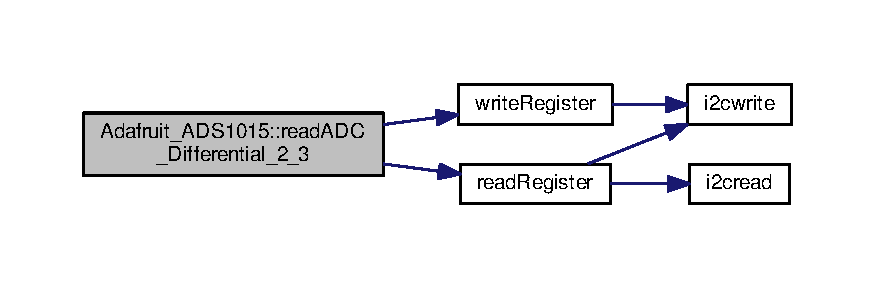
\includegraphics[width=350pt]{class_adafruit___a_d_s1015_a38311881bcab46f7496c4bb6e4cad576_cgraph}
\end{center}
\end{figure}
\mbox{\Hypertarget{class_adafruit___a_d_s1015_a40f38b9e1f3ec397c0670dd632510235}\label{class_adafruit___a_d_s1015_a40f38b9e1f3ec397c0670dd632510235}} 
\index{Adafruit\+\_\+\+A\+D\+S1015@{Adafruit\+\_\+\+A\+D\+S1015}!read\+A\+D\+C\+\_\+\+Single\+Ended@{read\+A\+D\+C\+\_\+\+Single\+Ended}}
\index{read\+A\+D\+C\+\_\+\+Single\+Ended@{read\+A\+D\+C\+\_\+\+Single\+Ended}!Adafruit\+\_\+\+A\+D\+S1015@{Adafruit\+\_\+\+A\+D\+S1015}}
\subsubsection{\texorpdfstring{read\+A\+D\+C\+\_\+\+Single\+Ended()}{readADC\_SingleEnded()}}
{\footnotesize\ttfamily uint16\+\_\+t Adafruit\+\_\+\+A\+D\+S1015\+::read\+A\+D\+C\+\_\+\+Single\+Ended (\begin{DoxyParamCaption}\item[{uint8\+\_\+t}]{channel }\end{DoxyParamCaption})}



Gets a single-\/ended A\+DC reading from the specified channel. 



Definition at line 143 of file Cool\+Adafruit\+\_\+\+A\+D\+S1015.\+cpp.

Here is the call graph for this function\+:\nopagebreak
\begin{figure}[H]
\begin{center}
\leavevmode
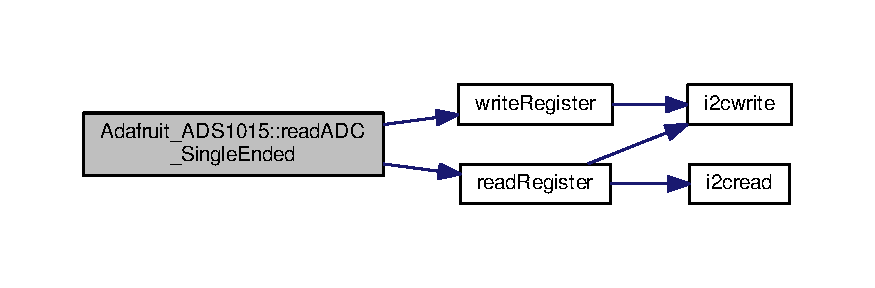
\includegraphics[width=350pt]{class_adafruit___a_d_s1015_a40f38b9e1f3ec397c0670dd632510235_cgraph}
\end{center}
\end{figure}
Here is the caller graph for this function\+:\nopagebreak
\begin{figure}[H]
\begin{center}
\leavevmode
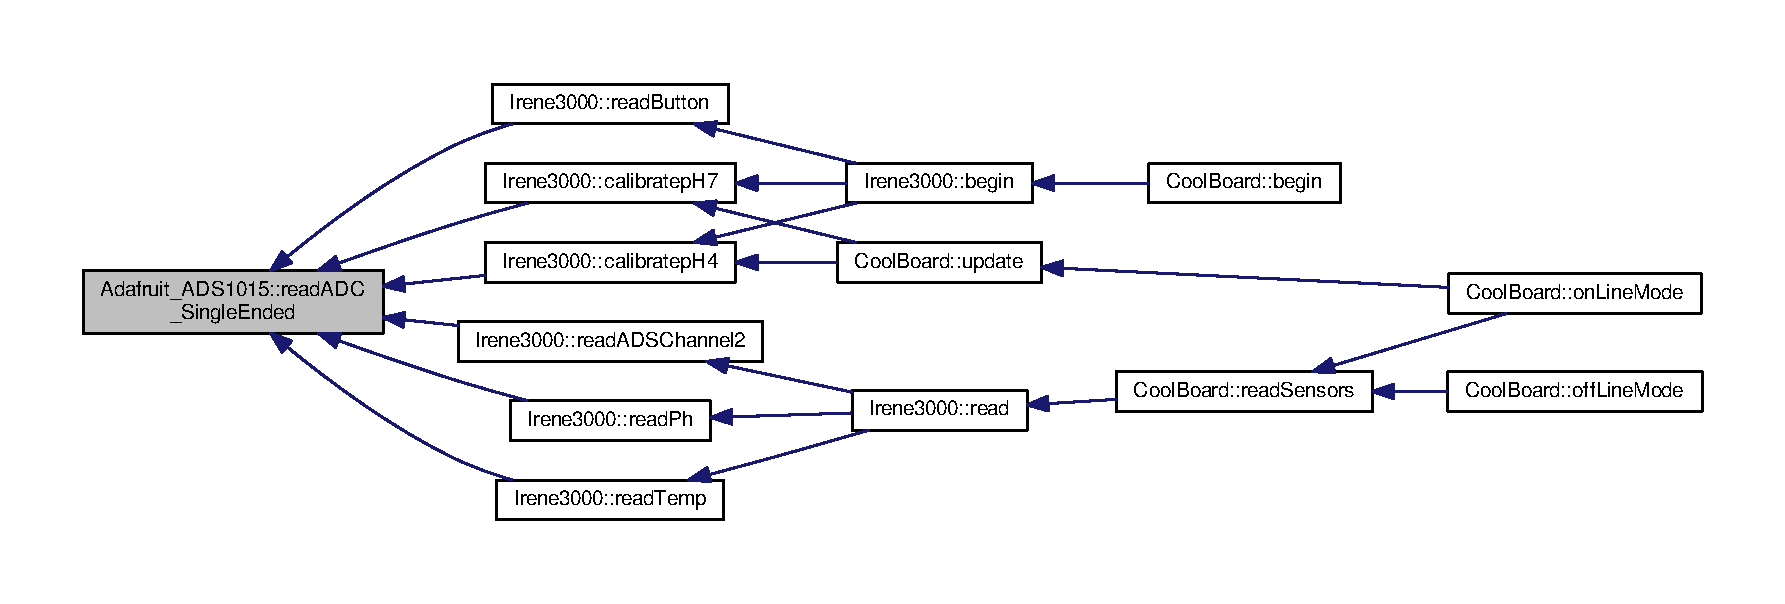
\includegraphics[width=350pt]{class_adafruit___a_d_s1015_a40f38b9e1f3ec397c0670dd632510235_icgraph}
\end{center}
\end{figure}
\mbox{\Hypertarget{class_adafruit___a_d_s1015_a399441eace686975ff22937cbe45cc50}\label{class_adafruit___a_d_s1015_a399441eace686975ff22937cbe45cc50}} 
\index{Adafruit\+\_\+\+A\+D\+S1015@{Adafruit\+\_\+\+A\+D\+S1015}!set\+Gain@{set\+Gain}}
\index{set\+Gain@{set\+Gain}!Adafruit\+\_\+\+A\+D\+S1015@{Adafruit\+\_\+\+A\+D\+S1015}}
\subsubsection{\texorpdfstring{set\+Gain()}{setGain()}}
{\footnotesize\ttfamily void Adafruit\+\_\+\+A\+D\+S1015\+::set\+Gain (\begin{DoxyParamCaption}\item[{\hyperlink{_cool_adafruit___a_d_s1015_8h_a3d6c0e15829a207b9155890811fa4781}{ads\+Gain\+\_\+t}}]{gain }\end{DoxyParamCaption})}



Sets the gain and input voltage range. 



Definition at line 123 of file Cool\+Adafruit\+\_\+\+A\+D\+S1015.\+cpp.

Here is the caller graph for this function\+:\nopagebreak
\begin{figure}[H]
\begin{center}
\leavevmode
\includegraphics[width=350pt]{class_adafruit___a_d_s1015_a399441eace686975ff22937cbe45cc50_icgraph}
\end{center}
\end{figure}
\mbox{\Hypertarget{class_adafruit___a_d_s1015_aecd30775d943ea9d9cff0e3485926596}\label{class_adafruit___a_d_s1015_aecd30775d943ea9d9cff0e3485926596}} 
\index{Adafruit\+\_\+\+A\+D\+S1015@{Adafruit\+\_\+\+A\+D\+S1015}!start\+Comparator\+\_\+\+Single\+Ended@{start\+Comparator\+\_\+\+Single\+Ended}}
\index{start\+Comparator\+\_\+\+Single\+Ended@{start\+Comparator\+\_\+\+Single\+Ended}!Adafruit\+\_\+\+A\+D\+S1015@{Adafruit\+\_\+\+A\+D\+S1015}}
\subsubsection{\texorpdfstring{start\+Comparator\+\_\+\+Single\+Ended()}{startComparator\_SingleEnded()}}
{\footnotesize\ttfamily void Adafruit\+\_\+\+A\+D\+S1015\+::start\+Comparator\+\_\+\+Single\+Ended (\begin{DoxyParamCaption}\item[{uint8\+\_\+t}]{channel,  }\item[{int16\+\_\+t}]{threshold }\end{DoxyParamCaption})}



Sets up the comparator to operate in basic mode, causing the A\+L\+E\+R\+T/\+R\+DY pin to assert (go from high to low) when the A\+DC value exceeds the specified threshold. 

This will also set the A\+DC in continuous conversion mode. 

Definition at line 302 of file Cool\+Adafruit\+\_\+\+A\+D\+S1015.\+cpp.

Here is the call graph for this function\+:\nopagebreak
\begin{figure}[H]
\begin{center}
\leavevmode
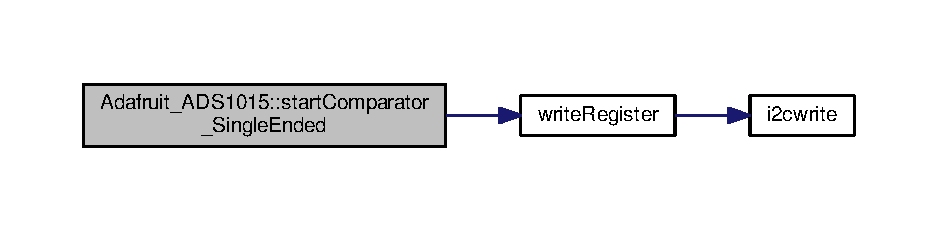
\includegraphics[width=350pt]{class_adafruit___a_d_s1015_aecd30775d943ea9d9cff0e3485926596_cgraph}
\end{center}
\end{figure}


\subsection{Member Data Documentation}
\mbox{\Hypertarget{class_adafruit___a_d_s1015_ab238ce17112a78db2be4ea14d57fb114}\label{class_adafruit___a_d_s1015_ab238ce17112a78db2be4ea14d57fb114}} 
\index{Adafruit\+\_\+\+A\+D\+S1015@{Adafruit\+\_\+\+A\+D\+S1015}!m\+\_\+bit\+Shift@{m\+\_\+bit\+Shift}}
\index{m\+\_\+bit\+Shift@{m\+\_\+bit\+Shift}!Adafruit\+\_\+\+A\+D\+S1015@{Adafruit\+\_\+\+A\+D\+S1015}}
\subsubsection{\texorpdfstring{m\+\_\+bit\+Shift}{m\_bitShift}}
{\footnotesize\ttfamily uint8\+\_\+t Adafruit\+\_\+\+A\+D\+S1015\+::m\+\_\+bit\+Shift\hspace{0.3cm}{\ttfamily [protected]}}



Definition at line 125 of file Cool\+Adafruit\+\_\+\+A\+D\+S1015.\+h.

\mbox{\Hypertarget{class_adafruit___a_d_s1015_aa3a29a64a6705fce1fee21d73c642a0e}\label{class_adafruit___a_d_s1015_aa3a29a64a6705fce1fee21d73c642a0e}} 
\index{Adafruit\+\_\+\+A\+D\+S1015@{Adafruit\+\_\+\+A\+D\+S1015}!m\+\_\+conversion\+Delay@{m\+\_\+conversion\+Delay}}
\index{m\+\_\+conversion\+Delay@{m\+\_\+conversion\+Delay}!Adafruit\+\_\+\+A\+D\+S1015@{Adafruit\+\_\+\+A\+D\+S1015}}
\subsubsection{\texorpdfstring{m\+\_\+conversion\+Delay}{m\_conversionDelay}}
{\footnotesize\ttfamily uint8\+\_\+t Adafruit\+\_\+\+A\+D\+S1015\+::m\+\_\+conversion\+Delay\hspace{0.3cm}{\ttfamily [protected]}}



Definition at line 124 of file Cool\+Adafruit\+\_\+\+A\+D\+S1015.\+h.

\mbox{\Hypertarget{class_adafruit___a_d_s1015_a8db90fe03d55a18246984ba2ba5e7f32}\label{class_adafruit___a_d_s1015_a8db90fe03d55a18246984ba2ba5e7f32}} 
\index{Adafruit\+\_\+\+A\+D\+S1015@{Adafruit\+\_\+\+A\+D\+S1015}!m\+\_\+gain@{m\+\_\+gain}}
\index{m\+\_\+gain@{m\+\_\+gain}!Adafruit\+\_\+\+A\+D\+S1015@{Adafruit\+\_\+\+A\+D\+S1015}}
\subsubsection{\texorpdfstring{m\+\_\+gain}{m\_gain}}
{\footnotesize\ttfamily \hyperlink{_cool_adafruit___a_d_s1015_8h_a3d6c0e15829a207b9155890811fa4781}{ads\+Gain\+\_\+t} Adafruit\+\_\+\+A\+D\+S1015\+::m\+\_\+gain\hspace{0.3cm}{\ttfamily [protected]}}



Definition at line 126 of file Cool\+Adafruit\+\_\+\+A\+D\+S1015.\+h.

\mbox{\Hypertarget{class_adafruit___a_d_s1015_a2186993621a7973256d47f086c74035d}\label{class_adafruit___a_d_s1015_a2186993621a7973256d47f086c74035d}} 
\index{Adafruit\+\_\+\+A\+D\+S1015@{Adafruit\+\_\+\+A\+D\+S1015}!m\+\_\+i2c\+Address@{m\+\_\+i2c\+Address}}
\index{m\+\_\+i2c\+Address@{m\+\_\+i2c\+Address}!Adafruit\+\_\+\+A\+D\+S1015@{Adafruit\+\_\+\+A\+D\+S1015}}
\subsubsection{\texorpdfstring{m\+\_\+i2c\+Address}{m\_i2cAddress}}
{\footnotesize\ttfamily uint8\+\_\+t Adafruit\+\_\+\+A\+D\+S1015\+::m\+\_\+i2c\+Address\hspace{0.3cm}{\ttfamily [protected]}}



Definition at line 123 of file Cool\+Adafruit\+\_\+\+A\+D\+S1015.\+h.



The documentation for this class was generated from the following files\+:\begin{DoxyCompactItemize}
\item 
/home/ashiroji/\+Arduino/libraries/\+Cool\+Board/src/internals/\hyperlink{_cool_adafruit___a_d_s1015_8h}{Cool\+Adafruit\+\_\+\+A\+D\+S1015.\+h}\item 
/home/ashiroji/\+Arduino/libraries/\+Cool\+Board/src/internals/\hyperlink{_cool_adafruit___a_d_s1015_8cpp}{Cool\+Adafruit\+\_\+\+A\+D\+S1015.\+cpp}\end{DoxyCompactItemize}

\hypertarget{class_adafruit___a_d_s1115}{}\section{Adafruit\+\_\+\+A\+D\+S1115 Class Reference}
\label{class_adafruit___a_d_s1115}\index{Adafruit\+\_\+\+A\+D\+S1115@{Adafruit\+\_\+\+A\+D\+S1115}}


{\ttfamily \#include $<$Cool\+Adafruit\+\_\+\+A\+D\+S1015.\+h$>$}



Inheritance diagram for Adafruit\+\_\+\+A\+D\+S1115\+:
\nopagebreak
\begin{figure}[H]
\begin{center}
\leavevmode
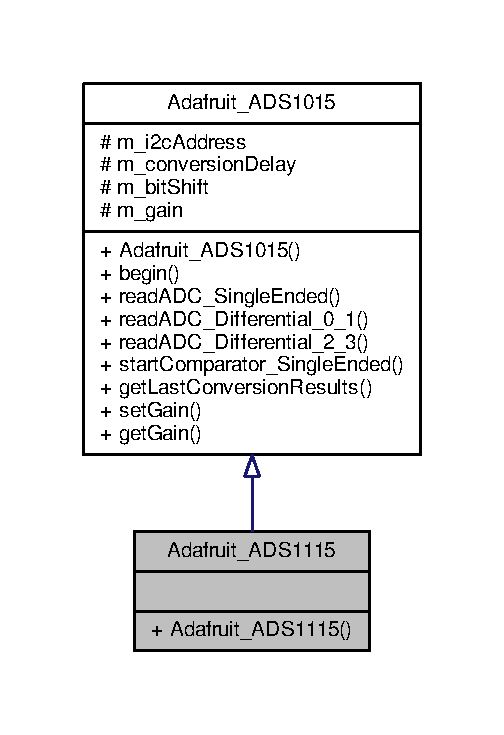
\includegraphics[width=242pt]{class_adafruit___a_d_s1115__inherit__graph}
\end{center}
\end{figure}


Collaboration diagram for Adafruit\+\_\+\+A\+D\+S1115\+:
\nopagebreak
\begin{figure}[H]
\begin{center}
\leavevmode
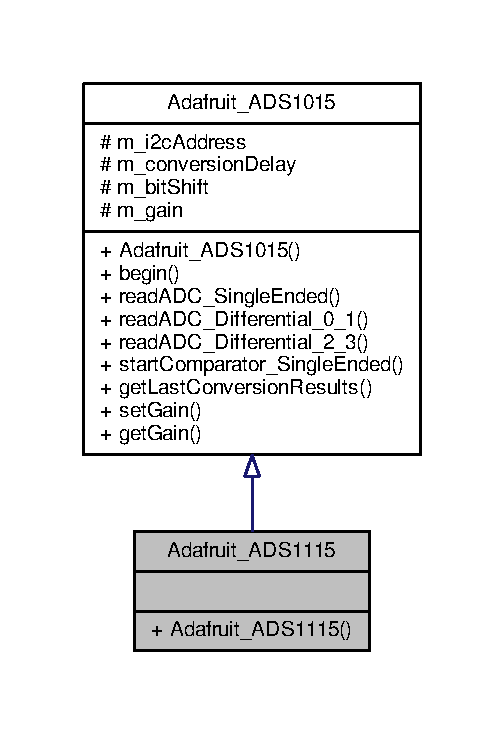
\includegraphics[width=242pt]{class_adafruit___a_d_s1115__coll__graph}
\end{center}
\end{figure}
\subsection*{Public Member Functions}
\begin{DoxyCompactItemize}
\item 
\hyperlink{class_adafruit___a_d_s1115_a7058cf2c75b673fb0b0a8936c3edd1fd}{Adafruit\+\_\+\+A\+D\+S1115} (uint8\+\_\+t i2c\+Address=\hyperlink{_cool_adafruit___a_d_s1015_8h_ae55d158023984e8f0ddc80b58d5b30dc}{A\+D\+S1015\+\_\+\+A\+D\+D\+R\+E\+SS})
\begin{DoxyCompactList}\small\item\em Instantiates a new A\+D\+S1115 class w/appropriate properties. \end{DoxyCompactList}\end{DoxyCompactItemize}
\subsection*{Additional Inherited Members}


\subsection{Detailed Description}


Definition at line 143 of file Cool\+Adafruit\+\_\+\+A\+D\+S1015.\+h.



\subsection{Constructor \& Destructor Documentation}
\mbox{\Hypertarget{class_adafruit___a_d_s1115_a7058cf2c75b673fb0b0a8936c3edd1fd}\label{class_adafruit___a_d_s1115_a7058cf2c75b673fb0b0a8936c3edd1fd}} 
\index{Adafruit\+\_\+\+A\+D\+S1115@{Adafruit\+\_\+\+A\+D\+S1115}!Adafruit\+\_\+\+A\+D\+S1115@{Adafruit\+\_\+\+A\+D\+S1115}}
\index{Adafruit\+\_\+\+A\+D\+S1115@{Adafruit\+\_\+\+A\+D\+S1115}!Adafruit\+\_\+\+A\+D\+S1115@{Adafruit\+\_\+\+A\+D\+S1115}}
\subsubsection{\texorpdfstring{Adafruit\+\_\+\+A\+D\+S1115()}{Adafruit\_ADS1115()}}
{\footnotesize\ttfamily Adafruit\+\_\+\+A\+D\+S1115\+::\+Adafruit\+\_\+\+A\+D\+S1115 (\begin{DoxyParamCaption}\item[{uint8\+\_\+t}]{i2c\+Address = {\ttfamily \hyperlink{_cool_adafruit___a_d_s1015_8h_ae55d158023984e8f0ddc80b58d5b30dc}{A\+D\+S1015\+\_\+\+A\+D\+D\+R\+E\+SS}} }\end{DoxyParamCaption})}



Instantiates a new A\+D\+S1115 class w/appropriate properties. 



Definition at line 101 of file Cool\+Adafruit\+\_\+\+A\+D\+S1015.\+cpp.



The documentation for this class was generated from the following files\+:\begin{DoxyCompactItemize}
\item 
/home/ashiroji/\+Arduino/libraries/\+Cool\+Board/src/internals/\hyperlink{_cool_adafruit___a_d_s1015_8h}{Cool\+Adafruit\+\_\+\+A\+D\+S1015.\+h}\item 
/home/ashiroji/\+Arduino/libraries/\+Cool\+Board/src/internals/\hyperlink{_cool_adafruit___a_d_s1015_8cpp}{Cool\+Adafruit\+\_\+\+A\+D\+S1015.\+cpp}\end{DoxyCompactItemize}

\hypertarget{struct_cool_board_sensors_1_1air_active}{}\section{Cool\+Board\+Sensors\+:\+:air\+Active Struct Reference}
\label{struct_cool_board_sensors_1_1air_active}\index{Cool\+Board\+Sensors\+::air\+Active@{Cool\+Board\+Sensors\+::air\+Active}}


Collaboration diagram for Cool\+Board\+Sensors\+:\+:air\+Active\+:\nopagebreak
\begin{figure}[H]
\begin{center}
\leavevmode
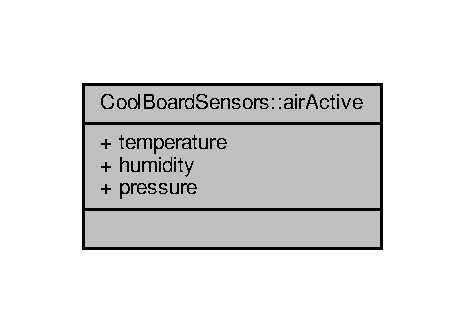
\includegraphics[width=223pt]{d5/d30/struct_cool_board_sensors_1_1air_active__coll__graph}
\end{center}
\end{figure}
\subsection*{Public Attributes}
\begin{DoxyCompactItemize}
\item 
byte \hyperlink{struct_cool_board_sensors_1_1air_active_a9a6633c426b0508e30ebc1832ec6d745}{temperature} =0
\item 
byte \hyperlink{struct_cool_board_sensors_1_1air_active_ae5740445054b27415e22f450576accb7}{humidity} =0
\item 
byte \hyperlink{struct_cool_board_sensors_1_1air_active_ab200826a70d1dc9945f5efb6b9c732ed}{pressure} =0
\end{DoxyCompactItemize}


\subsection{Detailed Description}


Definition at line 77 of file Cool\+Board\+Sensors.\+h.



\subsection{Member Data Documentation}
\mbox{\Hypertarget{struct_cool_board_sensors_1_1air_active_ae5740445054b27415e22f450576accb7}\label{struct_cool_board_sensors_1_1air_active_ae5740445054b27415e22f450576accb7}} 
\index{Cool\+Board\+Sensors\+::air\+Active@{Cool\+Board\+Sensors\+::air\+Active}!humidity@{humidity}}
\index{humidity@{humidity}!Cool\+Board\+Sensors\+::air\+Active@{Cool\+Board\+Sensors\+::air\+Active}}
\subsubsection{\texorpdfstring{humidity}{humidity}}
{\footnotesize\ttfamily byte Cool\+Board\+Sensors\+::air\+Active\+::humidity =0}



Definition at line 80 of file Cool\+Board\+Sensors.\+h.

\mbox{\Hypertarget{struct_cool_board_sensors_1_1air_active_ab200826a70d1dc9945f5efb6b9c732ed}\label{struct_cool_board_sensors_1_1air_active_ab200826a70d1dc9945f5efb6b9c732ed}} 
\index{Cool\+Board\+Sensors\+::air\+Active@{Cool\+Board\+Sensors\+::air\+Active}!pressure@{pressure}}
\index{pressure@{pressure}!Cool\+Board\+Sensors\+::air\+Active@{Cool\+Board\+Sensors\+::air\+Active}}
\subsubsection{\texorpdfstring{pressure}{pressure}}
{\footnotesize\ttfamily byte Cool\+Board\+Sensors\+::air\+Active\+::pressure =0}



Definition at line 81 of file Cool\+Board\+Sensors.\+h.

\mbox{\Hypertarget{struct_cool_board_sensors_1_1air_active_a9a6633c426b0508e30ebc1832ec6d745}\label{struct_cool_board_sensors_1_1air_active_a9a6633c426b0508e30ebc1832ec6d745}} 
\index{Cool\+Board\+Sensors\+::air\+Active@{Cool\+Board\+Sensors\+::air\+Active}!temperature@{temperature}}
\index{temperature@{temperature}!Cool\+Board\+Sensors\+::air\+Active@{Cool\+Board\+Sensors\+::air\+Active}}
\subsubsection{\texorpdfstring{temperature}{temperature}}
{\footnotesize\ttfamily byte Cool\+Board\+Sensors\+::air\+Active\+::temperature =0}



Definition at line 79 of file Cool\+Board\+Sensors.\+h.



The documentation for this struct was generated from the following file\+:\begin{DoxyCompactItemize}
\item 
/home/ashiroji/\+Arduino/libraries/\+Cool\+Board/src/\hyperlink{_cool_board_sensors_8h}{Cool\+Board\+Sensors.\+h}\end{DoxyCompactItemize}

\hypertarget{class_base_external_sensor}{}\section{Base\+External\+Sensor Class Reference}
\label{class_base_external_sensor}\index{Base\+External\+Sensor@{Base\+External\+Sensor}}


This class is a generic external Sensor it is a way to access real external sensor methods through run Time polymorphism.  




{\ttfamily \#include $<$External\+Sensor.\+h$>$}



Inheritance diagram for Base\+External\+Sensor\+:\nopagebreak
\begin{figure}[H]
\begin{center}
\leavevmode
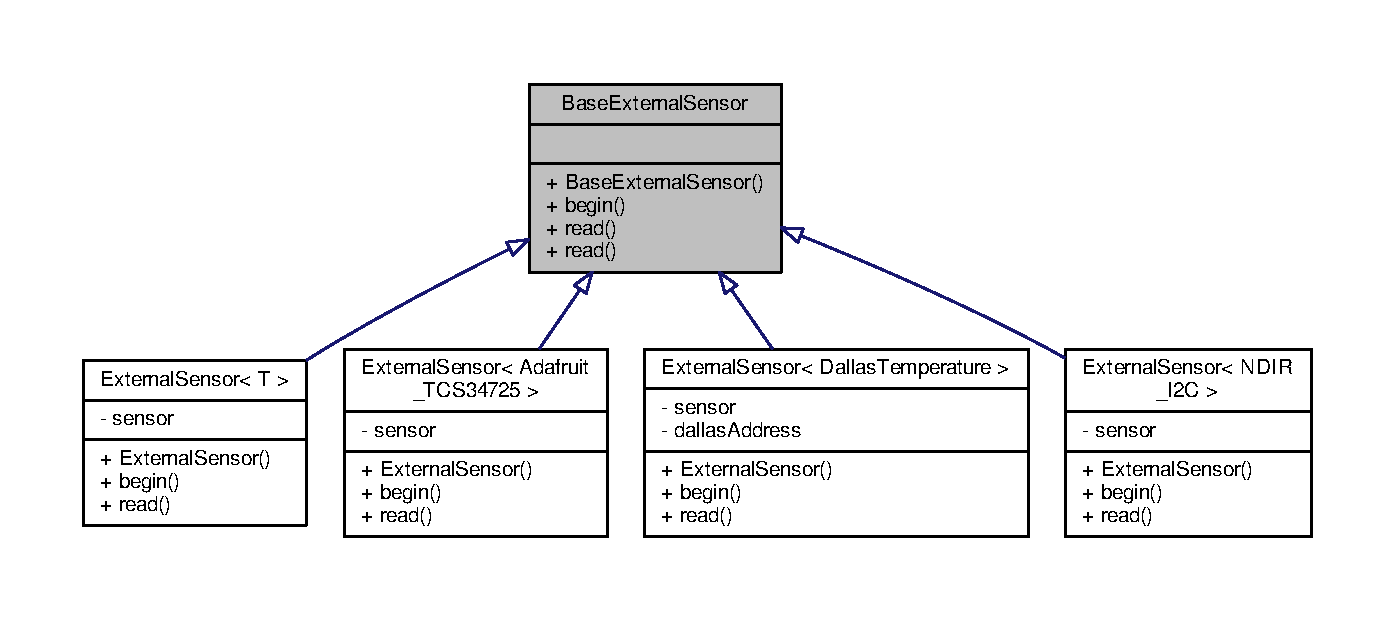
\includegraphics[width=350pt]{d5/d26/class_base_external_sensor__inherit__graph}
\end{center}
\end{figure}


Collaboration diagram for Base\+External\+Sensor\+:\nopagebreak
\begin{figure}[H]
\begin{center}
\leavevmode
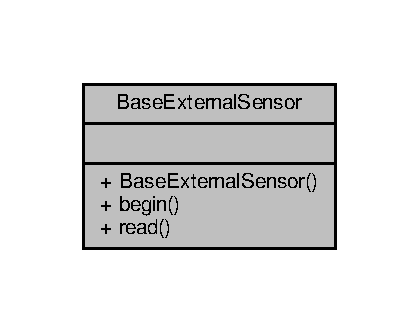
\includegraphics[width=201pt]{d4/dc4/class_base_external_sensor__coll__graph}
\end{center}
\end{figure}
\subsection*{Public Member Functions}
\begin{DoxyCompactItemize}
\item 
\hyperlink{class_base_external_sensor_a978d96a6563b646efb358c2790a9fc6f}{Base\+External\+Sensor} ()
\item 
virtual uint8\+\_\+t \hyperlink{class_base_external_sensor_a87d132803d4f4fdd4e66332809f0c9a0}{begin} ()
\item 
virtual float \hyperlink{class_base_external_sensor_a1564f16deacf57b51b9948ac29db4291}{read} ()
\end{DoxyCompactItemize}


\subsection{Detailed Description}
This class is a generic external Sensor it is a way to access real external sensor methods through run Time polymorphism. 

Definition at line 50 of file External\+Sensor.\+h.



\subsection{Constructor \& Destructor Documentation}
\mbox{\Hypertarget{class_base_external_sensor_a978d96a6563b646efb358c2790a9fc6f}\label{class_base_external_sensor_a978d96a6563b646efb358c2790a9fc6f}} 
\index{Base\+External\+Sensor@{Base\+External\+Sensor}!Base\+External\+Sensor@{Base\+External\+Sensor}}
\index{Base\+External\+Sensor@{Base\+External\+Sensor}!Base\+External\+Sensor@{Base\+External\+Sensor}}
\subsubsection{\texorpdfstring{Base\+External\+Sensor()}{BaseExternalSensor()}}
{\footnotesize\ttfamily Base\+External\+Sensor\+::\+Base\+External\+Sensor (\begin{DoxyParamCaption}{ }\end{DoxyParamCaption})\hspace{0.3cm}{\ttfamily [inline]}}

\hyperlink{class_base_external_sensor_a978d96a6563b646efb358c2790a9fc6f}{Base\+External\+Sensor()}\+: Base class generic Constructor 

Definition at line 58 of file External\+Sensor.\+h.


\begin{DoxyCode}
59     \{
60 
61 \textcolor{preprocessor}{    #if DEBUGExternal == 1 }
62 
63         Serial.println( \textcolor{stringliteral}{"BaseExternalSensor Constructor"} );
64         Serial.println();
65     
66 \textcolor{preprocessor}{    #endif}
67 
68     \}
\end{DoxyCode}


\subsection{Member Function Documentation}
\mbox{\Hypertarget{class_base_external_sensor_a87d132803d4f4fdd4e66332809f0c9a0}\label{class_base_external_sensor_a87d132803d4f4fdd4e66332809f0c9a0}} 
\index{Base\+External\+Sensor@{Base\+External\+Sensor}!begin@{begin}}
\index{begin@{begin}!Base\+External\+Sensor@{Base\+External\+Sensor}}
\subsubsection{\texorpdfstring{begin()}{begin()}}
{\footnotesize\ttfamily virtual uint8\+\_\+t Base\+External\+Sensor\+::begin (\begin{DoxyParamCaption}{ }\end{DoxyParamCaption})\hspace{0.3cm}{\ttfamily [inline]}, {\ttfamily [virtual]}}

\hyperlink{class_base_external_sensor_a87d132803d4f4fdd4e66332809f0c9a0}{begin()}\+: Base class virtual generic begin method

\begin{DoxyReturn}{Returns}
generic value as it\textquotesingle{}s not supposed to be used 
\end{DoxyReturn}


Reimplemented in \hyperlink{class_external_sensor_3_01_dallas_temperature_01_4_ac5275129b05e2ff8df45d5b222a661d9}{External\+Sensor$<$ Dallas\+Temperature $>$}, \hyperlink{class_external_sensor_3_01_n_d_i_r___i2_c_01_4_ac6f3614d94968ef0cc11b2b4d69cef03}{External\+Sensor$<$ N\+D\+I\+R\+\_\+\+I2\+C $>$}, and \hyperlink{class_external_sensor_ab6fe1379d55b656a048e0fba1e0a32e6}{External\+Sensor$<$ T $>$}.



Definition at line 78 of file External\+Sensor.\+h.


\begin{DoxyCode}
79     \{
80     
81 \textcolor{preprocessor}{    #if DEBUGExternal == 1 }
82     
83         Serial.println( \textcolor{stringliteral}{"BaseExternalSensor.begin()"} );
84         Serial.println();
85     
86 \textcolor{preprocessor}{    #endif}
87 
88         \textcolor{keywordflow}{return}(-2);
89     \}
\end{DoxyCode}
Here is the caller graph for this function\+:\nopagebreak
\begin{figure}[H]
\begin{center}
\leavevmode
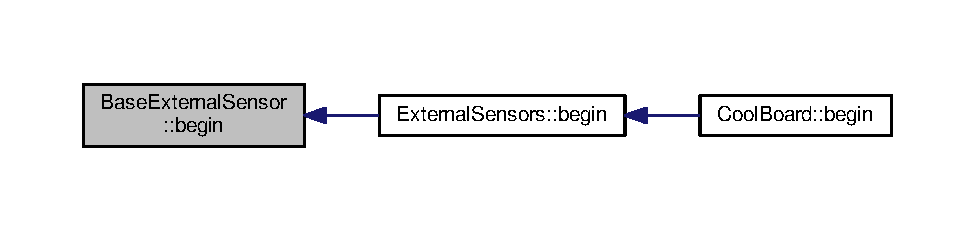
\includegraphics[width=350pt]{d1/d68/class_base_external_sensor_a87d132803d4f4fdd4e66332809f0c9a0_icgraph}
\end{center}
\end{figure}
\mbox{\Hypertarget{class_base_external_sensor_a1564f16deacf57b51b9948ac29db4291}\label{class_base_external_sensor_a1564f16deacf57b51b9948ac29db4291}} 
\index{Base\+External\+Sensor@{Base\+External\+Sensor}!read@{read}}
\index{read@{read}!Base\+External\+Sensor@{Base\+External\+Sensor}}
\subsubsection{\texorpdfstring{read()}{read()}}
{\footnotesize\ttfamily virtual float Base\+External\+Sensor\+::read (\begin{DoxyParamCaption}{ }\end{DoxyParamCaption})\hspace{0.3cm}{\ttfamily [inline]}, {\ttfamily [virtual]}}

\hyperlink{class_base_external_sensor_a1564f16deacf57b51b9948ac29db4291}{read()}\+: Base class virtual generic read method

\begin{DoxyReturn}{Returns}
generic value as it is not supposed to be used 
\end{DoxyReturn}


Reimplemented in \hyperlink{class_external_sensor_3_01_dallas_temperature_01_4_a1e725d9338314515d4e5dc456ed6a6c8}{External\+Sensor$<$ Dallas\+Temperature $>$}, \hyperlink{class_external_sensor_3_01_n_d_i_r___i2_c_01_4_a239d18652e9fb4673842ae9726edf44f}{External\+Sensor$<$ N\+D\+I\+R\+\_\+\+I2\+C $>$}, and \hyperlink{class_external_sensor_a5fb3afc7d244fb86dac68ab5481bc407}{External\+Sensor$<$ T $>$}.



Definition at line 100 of file External\+Sensor.\+h.


\begin{DoxyCode}
101     \{
102     
103 \textcolor{preprocessor}{    #if DEBUGExternal == 1 }
104 
105         Serial.println( \textcolor{stringliteral}{"BaseExternalSensor.read()"} );
106         Serial.println();
107     
108 \textcolor{preprocessor}{    #endif      }
109         
110         \textcolor{keywordflow}{return}(-2);
111     \}
\end{DoxyCode}
Here is the caller graph for this function\+:\nopagebreak
\begin{figure}[H]
\begin{center}
\leavevmode
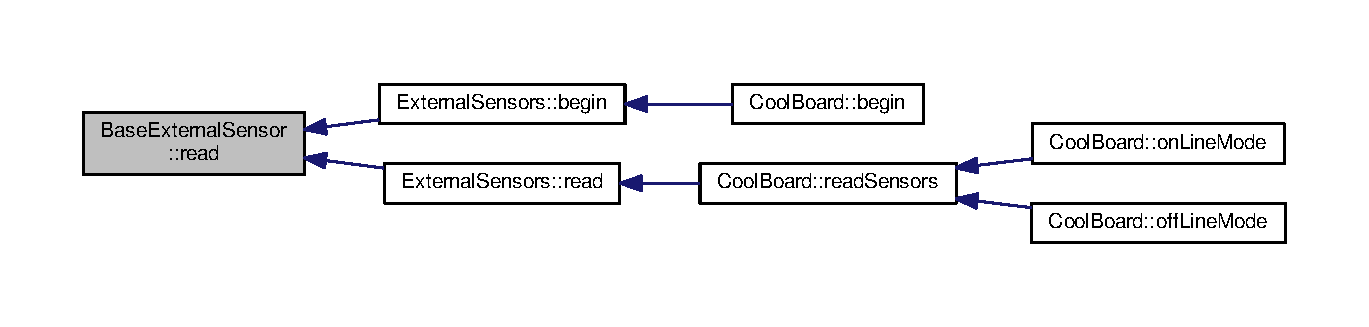
\includegraphics[width=350pt]{d1/d68/class_base_external_sensor_a1564f16deacf57b51b9948ac29db4291_icgraph}
\end{center}
\end{figure}


The documentation for this class was generated from the following file\+:\begin{DoxyCompactItemize}
\item 
/home/ashiroji/\+Arduino/libraries/\+Cool\+Board/src/\hyperlink{_external_sensor_8h}{External\+Sensor.\+h}\end{DoxyCompactItemize}

\hypertarget{class_b_m_e280}{}\section{B\+M\+E280 Class Reference}
\label{class_b_m_e280}\index{B\+M\+E280@{B\+M\+E280}}


{\ttfamily \#include $<$Cool\+Spark\+Fun\+B\+M\+E280.\+h$>$}



Collaboration diagram for B\+M\+E280\+:\nopagebreak
\begin{figure}[H]
\begin{center}
\leavevmode
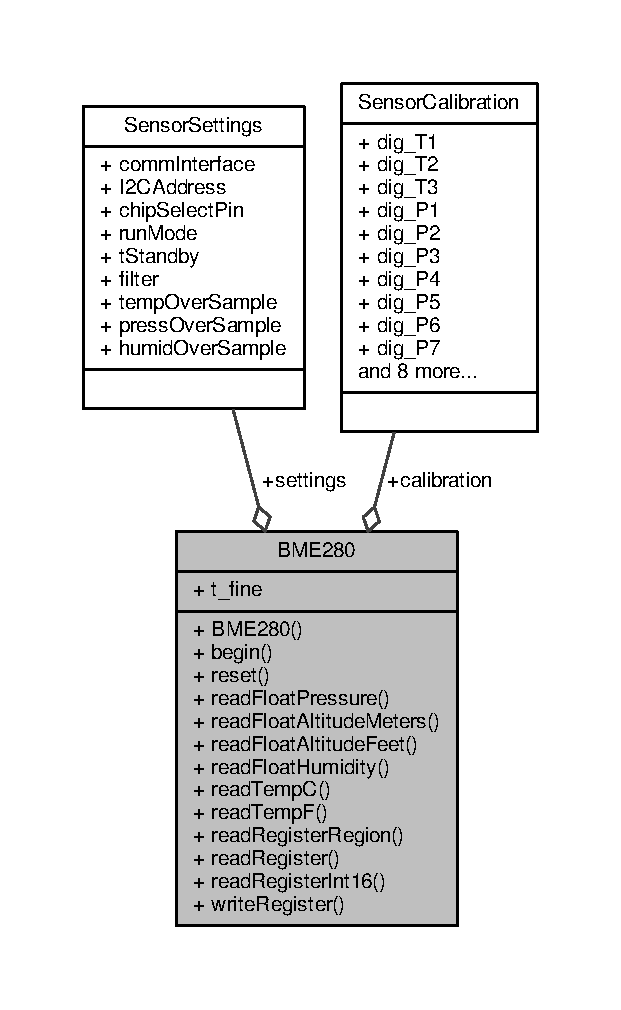
\includegraphics[width=298pt]{d3/d82/class_b_m_e280__coll__graph}
\end{center}
\end{figure}
\subsection*{Public Member Functions}
\begin{DoxyCompactItemize}
\item 
\hyperlink{class_b_m_e280_a9b9354e010528a0c3d452aa2459b808c}{B\+M\+E280} (void)
\item 
uint8\+\_\+t \hyperlink{class_b_m_e280_a994c102f010547f9c740a338ef9905c7}{begin} (void)
\item 
void \hyperlink{class_b_m_e280_aeec5deb6daace6ae390108b4210e9df7}{reset} (void)
\item 
float \hyperlink{class_b_m_e280_ada6e799917afb4f228e6253bc56ffe75}{read\+Float\+Pressure} (void)
\item 
float \hyperlink{class_b_m_e280_af67b56ba50760ee1d116acc6c5010221}{read\+Float\+Altitude\+Meters} (void)
\item 
float \hyperlink{class_b_m_e280_a6525c8a26f887b52596c86bed99343cb}{read\+Float\+Altitude\+Feet} (void)
\item 
float \hyperlink{class_b_m_e280_a42ea7232039eebf5aadb391ef6132c35}{read\+Float\+Humidity} (void)
\item 
float \hyperlink{class_b_m_e280_afffdd1d7ded9e1f92200e70669019d97}{read\+TempC} (void)
\item 
float \hyperlink{class_b_m_e280_a9648b496f6b4700550782a715a98b3c7}{read\+TempF} (void)
\item 
void \hyperlink{class_b_m_e280_aecca87c2c40a7f2bcabcea921bdc6124}{read\+Register\+Region} (uint8\+\_\+t $\ast$, uint8\+\_\+t, uint8\+\_\+t)
\item 
uint8\+\_\+t \hyperlink{class_b_m_e280_a1bbd14c8591966df531e40085342ff71}{read\+Register} (uint8\+\_\+t)
\item 
int16\+\_\+t \hyperlink{class_b_m_e280_ac43c30f9b321d301694094d6b4bebe7e}{read\+Register\+Int16} (uint8\+\_\+t offset)
\item 
void \hyperlink{class_b_m_e280_afcff21c342725246bf415d7f0e4d04f0}{write\+Register} (uint8\+\_\+t, uint8\+\_\+t)
\end{DoxyCompactItemize}
\subsection*{Public Attributes}
\begin{DoxyCompactItemize}
\item 
\hyperlink{struct_sensor_settings}{Sensor\+Settings} \hyperlink{class_b_m_e280_af06253eb2f8ad4b5fabb858bc4a973bf}{settings}
\item 
\hyperlink{struct_sensor_calibration}{Sensor\+Calibration} \hyperlink{class_b_m_e280_aa7a28484b6f5eb6f43261ea25016fbf8}{calibration}
\item 
int32\+\_\+t \hyperlink{class_b_m_e280_ad20f44914b78395f4d4bc64f4a68b369}{t\+\_\+fine}
\end{DoxyCompactItemize}


\subsection{Detailed Description}


Definition at line 143 of file Cool\+Spark\+Fun\+B\+M\+E280.\+h.



\subsection{Constructor \& Destructor Documentation}
\mbox{\Hypertarget{class_b_m_e280_a9b9354e010528a0c3d452aa2459b808c}\label{class_b_m_e280_a9b9354e010528a0c3d452aa2459b808c}} 
\index{B\+M\+E280@{B\+M\+E280}!B\+M\+E280@{B\+M\+E280}}
\index{B\+M\+E280@{B\+M\+E280}!B\+M\+E280@{B\+M\+E280}}
\subsubsection{\texorpdfstring{B\+M\+E280()}{BME280()}}
{\footnotesize\ttfamily B\+M\+E280\+::\+B\+M\+E280 (\begin{DoxyParamCaption}\item[{void}]{ }\end{DoxyParamCaption})}



Definition at line 43 of file Cool\+Spark\+Fun\+B\+M\+E280.\+cpp.


\begin{DoxyCode}
44 \{
45     \textcolor{comment}{//Construct with these default settings if nothing is specified}
46 
47     \textcolor{comment}{//Select interface mode}
48     \hyperlink{class_b_m_e280_af06253eb2f8ad4b5fabb858bc4a973bf}{settings}.\hyperlink{struct_sensor_settings_a5bf116387c543a6ea5732976424e8cb1}{commInterface} = \hyperlink{_cool_spark_fun_b_m_e280_8h_a5cd01756030509b764d43a2b8c94fce8}{I2C\_MODE}; \textcolor{comment}{//Can be I2C\_MODE, SPI\_MODE}
49     \textcolor{comment}{//Select address for I2C.  Does nothing for SPI}
50     \hyperlink{class_b_m_e280_af06253eb2f8ad4b5fabb858bc4a973bf}{settings}.\hyperlink{struct_sensor_settings_af8103021dbce7e5ee6d786c4893324f7}{I2CAddress} = 0x77; \textcolor{comment}{//Ignored for SPI\_MODE}
51     \textcolor{comment}{//Select CS pin for SPI.  Does nothing for I2C}
52     \hyperlink{class_b_m_e280_af06253eb2f8ad4b5fabb858bc4a973bf}{settings}.\hyperlink{struct_sensor_settings_abe2de606ebb580ad81e3fafb1a454580}{chipSelectPin} = 10;
53     \hyperlink{class_b_m_e280_af06253eb2f8ad4b5fabb858bc4a973bf}{settings}.\hyperlink{struct_sensor_settings_a0ffbdf34f4c23a2a167f00e4cb971dec}{runMode} = 0;
54     \hyperlink{class_b_m_e280_af06253eb2f8ad4b5fabb858bc4a973bf}{settings}.\hyperlink{struct_sensor_settings_abdedc9d05f4850c58005313486958073}{tempOverSample} = 0;
55     \hyperlink{class_b_m_e280_af06253eb2f8ad4b5fabb858bc4a973bf}{settings}.\hyperlink{struct_sensor_settings_a85ba10cad25b479bba9cb42c6400ab21}{pressOverSample} = 0;
56     \hyperlink{class_b_m_e280_af06253eb2f8ad4b5fabb858bc4a973bf}{settings}.\hyperlink{struct_sensor_settings_a4a02fc7708071b88ccf610e3f7ed9d55}{humidOverSample} = 0;
57 
58 \}
\end{DoxyCode}


\subsection{Member Function Documentation}
\mbox{\Hypertarget{class_b_m_e280_a994c102f010547f9c740a338ef9905c7}\label{class_b_m_e280_a994c102f010547f9c740a338ef9905c7}} 
\index{B\+M\+E280@{B\+M\+E280}!begin@{begin}}
\index{begin@{begin}!B\+M\+E280@{B\+M\+E280}}
\subsubsection{\texorpdfstring{begin()}{begin()}}
{\footnotesize\ttfamily uint8\+\_\+t B\+M\+E280\+::begin (\begin{DoxyParamCaption}\item[{void}]{ }\end{DoxyParamCaption})}



Definition at line 70 of file Cool\+Spark\+Fun\+B\+M\+E280.\+cpp.


\begin{DoxyCode}
71 \{
72     \textcolor{comment}{//Check the settings structure values to determine how to setup the device}
73     uint8\_t dataToWrite = 0;  \textcolor{comment}{//Temporary variable}
74 
75     \textcolor{keywordflow}{switch} (\hyperlink{class_b_m_e280_af06253eb2f8ad4b5fabb858bc4a973bf}{settings}.\hyperlink{struct_sensor_settings_a5bf116387c543a6ea5732976424e8cb1}{commInterface})
76     \{
77 
78     \textcolor{keywordflow}{case} \hyperlink{_cool_spark_fun_b_m_e280_8h_a5cd01756030509b764d43a2b8c94fce8}{I2C\_MODE}:
79         Wire.begin(2,14);
80         \textcolor{keywordflow}{break};
81 
82     \textcolor{keywordflow}{case} \hyperlink{_cool_spark_fun_b_m_e280_8h_ab1dcc9464e3fcb94922386e8a7f53f21}{SPI\_MODE}:
83         \textcolor{comment}{// start the SPI library:}
84         SPI.begin();
85         \textcolor{comment}{// Maximum SPI frequency is 10MHz, could divide by 2 here:}
86         SPI.setClockDivider(SPI\_CLOCK\_DIV32);
87         \textcolor{comment}{// Data is read and written MSb first.}
88         SPI.setBitOrder(MSBFIRST);
89         \textcolor{comment}{// Data is captured on rising edge of clock (CPHA = 0)}
90         \textcolor{comment}{// Base value of the clock is HIGH (CPOL = 1)}
91         \textcolor{comment}{// This was SPI\_MODE3 for RedBoard, but I had to change to}
92         \textcolor{comment}{// MODE0 for Teensy 3.1 operation}
93         SPI.setDataMode(SPI\_MODE3);
94         \textcolor{comment}{// initalize the  data ready and chip select pins:}
95         pinMode(\hyperlink{class_b_m_e280_af06253eb2f8ad4b5fabb858bc4a973bf}{settings}.\hyperlink{struct_sensor_settings_abe2de606ebb580ad81e3fafb1a454580}{chipSelectPin}, OUTPUT);
96         digitalWrite(\hyperlink{class_b_m_e280_af06253eb2f8ad4b5fabb858bc4a973bf}{settings}.\hyperlink{struct_sensor_settings_abe2de606ebb580ad81e3fafb1a454580}{chipSelectPin}, HIGH);
97         \textcolor{keywordflow}{break};
98 
99     \textcolor{keywordflow}{default}:
100         \textcolor{keywordflow}{break};
101     \}
102 
103     \textcolor{comment}{//Reading all compensation data, range 0x88:A1, 0xE1:E7}
104     
105     \hyperlink{class_b_m_e280_aa7a28484b6f5eb6f43261ea25016fbf8}{calibration}.\hyperlink{struct_sensor_calibration_a044a8c40e958b1cda3fb85b95303550e}{dig\_T1} = ((uint16\_t)((\hyperlink{class_b_m_e280_a1bbd14c8591966df531e40085342ff71}{readRegister}(
      \hyperlink{_cool_spark_fun_b_m_e280_8h_ab41e00320fc3817544911020c4892ce9}{BME280\_DIG\_T1\_MSB\_REG}) << 8) + \hyperlink{class_b_m_e280_a1bbd14c8591966df531e40085342ff71}{readRegister}(
      \hyperlink{_cool_spark_fun_b_m_e280_8h_a95bded41d4d21e0dc9d5e90cef46e2f0}{BME280\_DIG\_T1\_LSB\_REG})));
106     \hyperlink{class_b_m_e280_aa7a28484b6f5eb6f43261ea25016fbf8}{calibration}.\hyperlink{struct_sensor_calibration_a8f8bb62e10c9bc0decb4463128ccaee5}{dig\_T2} = ((int16\_t)((\hyperlink{class_b_m_e280_a1bbd14c8591966df531e40085342ff71}{readRegister}(
      \hyperlink{_cool_spark_fun_b_m_e280_8h_a04dadb44784187c69a905720ce955e84}{BME280\_DIG\_T2\_MSB\_REG}) << 8) + \hyperlink{class_b_m_e280_a1bbd14c8591966df531e40085342ff71}{readRegister}(
      \hyperlink{_cool_spark_fun_b_m_e280_8h_aeb987cec0df70171e3f36e5d3b68f57b}{BME280\_DIG\_T2\_LSB\_REG})));
107     \hyperlink{class_b_m_e280_aa7a28484b6f5eb6f43261ea25016fbf8}{calibration}.\hyperlink{struct_sensor_calibration_a5b134db1776888487855c6b526d130d6}{dig\_T3} = ((int16\_t)((\hyperlink{class_b_m_e280_a1bbd14c8591966df531e40085342ff71}{readRegister}(
      \hyperlink{_cool_spark_fun_b_m_e280_8h_a656d326254d65330c2bdf9482ca590fc}{BME280\_DIG\_T3\_MSB\_REG}) << 8) + \hyperlink{class_b_m_e280_a1bbd14c8591966df531e40085342ff71}{readRegister}(
      \hyperlink{_cool_spark_fun_b_m_e280_8h_aa900c543759fa27e583393ef8740c37a}{BME280\_DIG\_T3\_LSB\_REG})));
108 
109     \hyperlink{class_b_m_e280_aa7a28484b6f5eb6f43261ea25016fbf8}{calibration}.\hyperlink{struct_sensor_calibration_aba96e3c2bdbbe79c20a836d9c55c60cf}{dig\_P1} = ((uint16\_t)((\hyperlink{class_b_m_e280_a1bbd14c8591966df531e40085342ff71}{readRegister}(
      \hyperlink{_cool_spark_fun_b_m_e280_8h_ad521625b8228f27c5bd1408f11c82705}{BME280\_DIG\_P1\_MSB\_REG}) << 8) + \hyperlink{class_b_m_e280_a1bbd14c8591966df531e40085342ff71}{readRegister}(
      \hyperlink{_cool_spark_fun_b_m_e280_8h_a4e93de21dbe08f37e606c40c9fc144d0}{BME280\_DIG\_P1\_LSB\_REG})));
110     \hyperlink{class_b_m_e280_aa7a28484b6f5eb6f43261ea25016fbf8}{calibration}.\hyperlink{struct_sensor_calibration_ab8a514b812ec77913dc95147d66bbcc4}{dig\_P2} = ((int16\_t)((\hyperlink{class_b_m_e280_a1bbd14c8591966df531e40085342ff71}{readRegister}(
      \hyperlink{_cool_spark_fun_b_m_e280_8h_afa34e3a536046bc6156a1ed4bb507d95}{BME280\_DIG\_P2\_MSB\_REG}) << 8) + \hyperlink{class_b_m_e280_a1bbd14c8591966df531e40085342ff71}{readRegister}(
      \hyperlink{_cool_spark_fun_b_m_e280_8h_a413900b0f4aa9c057203f6b198e78806}{BME280\_DIG\_P2\_LSB\_REG})));
111     \hyperlink{class_b_m_e280_aa7a28484b6f5eb6f43261ea25016fbf8}{calibration}.\hyperlink{struct_sensor_calibration_ac333ef210929de18815cec04c68acec2}{dig\_P3} = ((int16\_t)((\hyperlink{class_b_m_e280_a1bbd14c8591966df531e40085342ff71}{readRegister}(
      \hyperlink{_cool_spark_fun_b_m_e280_8h_a37526ca63d516cbca0117a54e9266190}{BME280\_DIG\_P3\_MSB\_REG}) << 8) + \hyperlink{class_b_m_e280_a1bbd14c8591966df531e40085342ff71}{readRegister}(
      \hyperlink{_cool_spark_fun_b_m_e280_8h_adcc5e52670f45b9f63a9135c5e1c5492}{BME280\_DIG\_P3\_LSB\_REG})));
112     \hyperlink{class_b_m_e280_aa7a28484b6f5eb6f43261ea25016fbf8}{calibration}.\hyperlink{struct_sensor_calibration_a8af2a8c6f19a2a56e784aa9a7bd49cd3}{dig\_P4} = ((int16\_t)((\hyperlink{class_b_m_e280_a1bbd14c8591966df531e40085342ff71}{readRegister}(
      \hyperlink{_cool_spark_fun_b_m_e280_8h_a7df62b54283c277da20b12bb322870e0}{BME280\_DIG\_P4\_MSB\_REG}) << 8) + \hyperlink{class_b_m_e280_a1bbd14c8591966df531e40085342ff71}{readRegister}(
      \hyperlink{_cool_spark_fun_b_m_e280_8h_a74ecf31c885677d4d6b8a3d8db22ee6d}{BME280\_DIG\_P4\_LSB\_REG})));
113     \hyperlink{class_b_m_e280_aa7a28484b6f5eb6f43261ea25016fbf8}{calibration}.\hyperlink{struct_sensor_calibration_ae2508256bbfc0e222a677ebbd1d0acf7}{dig\_P5} = ((int16\_t)((\hyperlink{class_b_m_e280_a1bbd14c8591966df531e40085342ff71}{readRegister}(
      \hyperlink{_cool_spark_fun_b_m_e280_8h_ac038f66828c72b71559096efafa76970}{BME280\_DIG\_P5\_MSB\_REG}) << 8) + \hyperlink{class_b_m_e280_a1bbd14c8591966df531e40085342ff71}{readRegister}(
      \hyperlink{_cool_spark_fun_b_m_e280_8h_a7054983fb5c397ec63838d2b6d047a12}{BME280\_DIG\_P5\_LSB\_REG})));
114     \hyperlink{class_b_m_e280_aa7a28484b6f5eb6f43261ea25016fbf8}{calibration}.\hyperlink{struct_sensor_calibration_ad1a973f775ee6d7f23d9197824971c76}{dig\_P6} = ((int16\_t)((\hyperlink{class_b_m_e280_a1bbd14c8591966df531e40085342ff71}{readRegister}(
      \hyperlink{_cool_spark_fun_b_m_e280_8h_ac43647d729a7d57221ecb0cf139accb4}{BME280\_DIG\_P6\_MSB\_REG}) << 8) + \hyperlink{class_b_m_e280_a1bbd14c8591966df531e40085342ff71}{readRegister}(
      \hyperlink{_cool_spark_fun_b_m_e280_8h_a7e12334e305f1665cbcaa02bdbb38909}{BME280\_DIG\_P6\_LSB\_REG})));
115     \hyperlink{class_b_m_e280_aa7a28484b6f5eb6f43261ea25016fbf8}{calibration}.\hyperlink{struct_sensor_calibration_adda4a99343f9e02de7d9f2d5949477d2}{dig\_P7} = ((int16\_t)((\hyperlink{class_b_m_e280_a1bbd14c8591966df531e40085342ff71}{readRegister}(
      \hyperlink{_cool_spark_fun_b_m_e280_8h_a7587b0d965b303fec2c2d4371add623f}{BME280\_DIG\_P7\_MSB\_REG}) << 8) + \hyperlink{class_b_m_e280_a1bbd14c8591966df531e40085342ff71}{readRegister}(
      \hyperlink{_cool_spark_fun_b_m_e280_8h_a70f6683a4c3c0818405ca3880f28a109}{BME280\_DIG\_P7\_LSB\_REG})));
116     \hyperlink{class_b_m_e280_aa7a28484b6f5eb6f43261ea25016fbf8}{calibration}.\hyperlink{struct_sensor_calibration_a06372d2918206f0cd35954e5bb35a1d2}{dig\_P8} = ((int16\_t)((\hyperlink{class_b_m_e280_a1bbd14c8591966df531e40085342ff71}{readRegister}(
      \hyperlink{_cool_spark_fun_b_m_e280_8h_a26633dd2c5b34de0d5163e11f9e3a22d}{BME280\_DIG\_P8\_MSB\_REG}) << 8) + \hyperlink{class_b_m_e280_a1bbd14c8591966df531e40085342ff71}{readRegister}(
      \hyperlink{_cool_spark_fun_b_m_e280_8h_afe625f2ec64c74d6488a93ba04575b24}{BME280\_DIG\_P8\_LSB\_REG})));
117     \hyperlink{class_b_m_e280_aa7a28484b6f5eb6f43261ea25016fbf8}{calibration}.\hyperlink{struct_sensor_calibration_a5e942a51a1b5d7753719db1e27e55c06}{dig\_P9} = ((int16\_t)((\hyperlink{class_b_m_e280_a1bbd14c8591966df531e40085342ff71}{readRegister}(
      \hyperlink{_cool_spark_fun_b_m_e280_8h_a819382b7d14efff4294e19f9a72010b3}{BME280\_DIG\_P9\_MSB\_REG}) << 8) + \hyperlink{class_b_m_e280_a1bbd14c8591966df531e40085342ff71}{readRegister}(
      \hyperlink{_cool_spark_fun_b_m_e280_8h_a24f19ebc8092ddede86f5533b9f09313}{BME280\_DIG\_P9\_LSB\_REG})));
118 
119     \hyperlink{class_b_m_e280_aa7a28484b6f5eb6f43261ea25016fbf8}{calibration}.\hyperlink{struct_sensor_calibration_ab8de0d58f5b0efa7ce638bed02deb460}{dig\_H1} = ((uint8\_t)(\hyperlink{class_b_m_e280_a1bbd14c8591966df531e40085342ff71}{readRegister}(
      \hyperlink{_cool_spark_fun_b_m_e280_8h_ad29dd403735dc3c3225c6838e5eed820}{BME280\_DIG\_H1\_REG})));
120     \hyperlink{class_b_m_e280_aa7a28484b6f5eb6f43261ea25016fbf8}{calibration}.\hyperlink{struct_sensor_calibration_afcfd149e907f83effaee0ae5dfa82a8f}{dig\_H2} = ((int16\_t)((\hyperlink{class_b_m_e280_a1bbd14c8591966df531e40085342ff71}{readRegister}(
      \hyperlink{_cool_spark_fun_b_m_e280_8h_aaf8b4172339b971f5a5b108c98d5d2fe}{BME280\_DIG\_H2\_MSB\_REG}) << 8) + \hyperlink{class_b_m_e280_a1bbd14c8591966df531e40085342ff71}{readRegister}(
      \hyperlink{_cool_spark_fun_b_m_e280_8h_a260ba9aa4ae925ed4a76a2f45a62e1f2}{BME280\_DIG\_H2\_LSB\_REG})));
121     \hyperlink{class_b_m_e280_aa7a28484b6f5eb6f43261ea25016fbf8}{calibration}.\hyperlink{struct_sensor_calibration_a65b525f9a3c58baf03db61da4626f417}{dig\_H3} = ((uint8\_t)(\hyperlink{class_b_m_e280_a1bbd14c8591966df531e40085342ff71}{readRegister}(
      \hyperlink{_cool_spark_fun_b_m_e280_8h_adbb9946cb6a096b6ff1f0226c0e7a659}{BME280\_DIG\_H3\_REG})));
122     \hyperlink{class_b_m_e280_aa7a28484b6f5eb6f43261ea25016fbf8}{calibration}.\hyperlink{struct_sensor_calibration_a6b540f7bc56275b482d65e0725aeb27b}{dig\_H4} = ((int16\_t)((\hyperlink{class_b_m_e280_a1bbd14c8591966df531e40085342ff71}{readRegister}(
      \hyperlink{_cool_spark_fun_b_m_e280_8h_a8dc154fcd1e08088d289ce668c4d718a}{BME280\_DIG\_H4\_MSB\_REG}) << 4) + (\hyperlink{class_b_m_e280_a1bbd14c8591966df531e40085342ff71}{readRegister}(
      \hyperlink{_cool_spark_fun_b_m_e280_8h_a722ff6a68e3db9eec127b191f2530a20}{BME280\_DIG\_H4\_LSB\_REG}) & 0x0F)));
123     \hyperlink{class_b_m_e280_aa7a28484b6f5eb6f43261ea25016fbf8}{calibration}.\hyperlink{struct_sensor_calibration_a03691fc56b0bff17b007ffbd71dcc7b9}{dig\_H5} = ((int16\_t)((\hyperlink{class_b_m_e280_a1bbd14c8591966df531e40085342ff71}{readRegister}(
      \hyperlink{_cool_spark_fun_b_m_e280_8h_ae7e42b75f0268a4303b77699fb8be834}{BME280\_DIG\_H5\_MSB\_REG}) << 4) + ((\hyperlink{class_b_m_e280_a1bbd14c8591966df531e40085342ff71}{readRegister}(
      \hyperlink{_cool_spark_fun_b_m_e280_8h_a722ff6a68e3db9eec127b191f2530a20}{BME280\_DIG\_H4\_LSB\_REG}) >> 4) & 0x0F)));
124     \hyperlink{class_b_m_e280_aa7a28484b6f5eb6f43261ea25016fbf8}{calibration}.\hyperlink{struct_sensor_calibration_a2f8c842c4becfce11e04c00168a9be0f}{dig\_H6} = ((uint8\_t)\hyperlink{class_b_m_e280_a1bbd14c8591966df531e40085342ff71}{readRegister}(
      \hyperlink{_cool_spark_fun_b_m_e280_8h_aa53163d82db48577fdb9a83112226e2c}{BME280\_DIG\_H6\_REG}));
125 
126     \textcolor{comment}{//Set the oversampling control words.}
127     \textcolor{comment}{//config will only be writeable in sleep mode, so first insure that.}
128     \hyperlink{class_b_m_e280_afcff21c342725246bf415d7f0e4d04f0}{writeRegister}(\hyperlink{_cool_spark_fun_b_m_e280_8h_a34483b4a562393f91fe3f01d676abb88}{BME280\_CTRL\_MEAS\_REG}, 0x00);
129     
130     \textcolor{comment}{//Set the config word}
131     dataToWrite = (\hyperlink{class_b_m_e280_af06253eb2f8ad4b5fabb858bc4a973bf}{settings}.\hyperlink{struct_sensor_settings_a7098be3c1df0271dc9bc0fb45c1e9bb9}{tStandby} << 0x5) & 0xE0;
132     dataToWrite |= (\hyperlink{class_b_m_e280_af06253eb2f8ad4b5fabb858bc4a973bf}{settings}.\hyperlink{struct_sensor_settings_a69dc95368069a0f408a141d4c2cbf045}{filter} << 0x02) & 0x1C;
133     \hyperlink{class_b_m_e280_afcff21c342725246bf415d7f0e4d04f0}{writeRegister}(\hyperlink{_cool_spark_fun_b_m_e280_8h_a70c225069ef92e5da90ee45362f7ba69}{BME280\_CONFIG\_REG}, dataToWrite);
134     
135     \textcolor{comment}{//Set ctrl\_hum first, then ctrl\_meas to activate ctrl\_hum}
136     dataToWrite = \hyperlink{class_b_m_e280_af06253eb2f8ad4b5fabb858bc4a973bf}{settings}.\hyperlink{struct_sensor_settings_a4a02fc7708071b88ccf610e3f7ed9d55}{humidOverSample} & 0x07; \textcolor{comment}{//all other bits can be ignored}
137     \hyperlink{class_b_m_e280_afcff21c342725246bf415d7f0e4d04f0}{writeRegister}(\hyperlink{_cool_spark_fun_b_m_e280_8h_a6da31fc4446b80cf5a830a5df45a5743}{BME280\_CTRL\_HUMIDITY\_REG}, dataToWrite);
138     
139     \textcolor{comment}{//set ctrl\_meas}
140     \textcolor{comment}{//First, set temp oversampling}
141     dataToWrite = (\hyperlink{class_b_m_e280_af06253eb2f8ad4b5fabb858bc4a973bf}{settings}.\hyperlink{struct_sensor_settings_abdedc9d05f4850c58005313486958073}{tempOverSample} << 0x5) & 0xE0;
142     \textcolor{comment}{//Next, pressure oversampling}
143     dataToWrite |= (\hyperlink{class_b_m_e280_af06253eb2f8ad4b5fabb858bc4a973bf}{settings}.\hyperlink{struct_sensor_settings_a85ba10cad25b479bba9cb42c6400ab21}{pressOverSample} << 0x02) & 0x1C;
144     \textcolor{comment}{//Last, set mode}
145     dataToWrite |= (\hyperlink{class_b_m_e280_af06253eb2f8ad4b5fabb858bc4a973bf}{settings}.\hyperlink{struct_sensor_settings_a0ffbdf34f4c23a2a167f00e4cb971dec}{runMode}) & 0x03;
146     \textcolor{comment}{//Load the byte}
147     \hyperlink{class_b_m_e280_afcff21c342725246bf415d7f0e4d04f0}{writeRegister}(\hyperlink{_cool_spark_fun_b_m_e280_8h_a34483b4a562393f91fe3f01d676abb88}{BME280\_CTRL\_MEAS\_REG}, dataToWrite);
148     
149     \textcolor{keywordflow}{return} \hyperlink{class_b_m_e280_a1bbd14c8591966df531e40085342ff71}{readRegister}(0xD0);
150 \}
\end{DoxyCode}
Here is the call graph for this function\+:\nopagebreak
\begin{figure}[H]
\begin{center}
\leavevmode
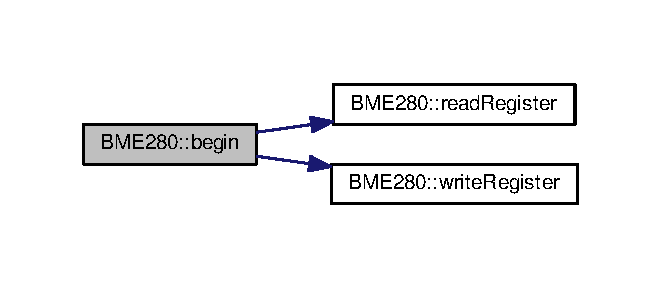
\includegraphics[width=317pt]{df/dcf/class_b_m_e280_a994c102f010547f9c740a338ef9905c7_cgraph}
\end{center}
\end{figure}
Here is the caller graph for this function\+:\nopagebreak
\begin{figure}[H]
\begin{center}
\leavevmode
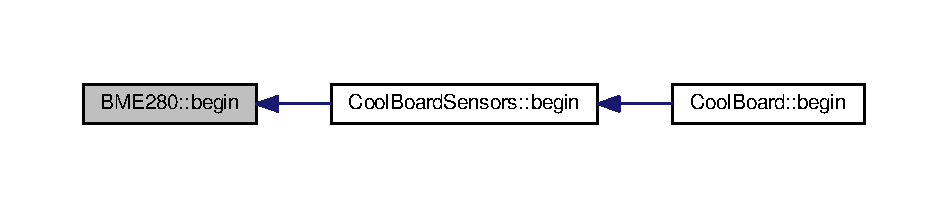
\includegraphics[width=350pt]{df/dcf/class_b_m_e280_a994c102f010547f9c740a338ef9905c7_icgraph}
\end{center}
\end{figure}
\mbox{\Hypertarget{class_b_m_e280_a6525c8a26f887b52596c86bed99343cb}\label{class_b_m_e280_a6525c8a26f887b52596c86bed99343cb}} 
\index{B\+M\+E280@{B\+M\+E280}!read\+Float\+Altitude\+Feet@{read\+Float\+Altitude\+Feet}}
\index{read\+Float\+Altitude\+Feet@{read\+Float\+Altitude\+Feet}!B\+M\+E280@{B\+M\+E280}}
\subsubsection{\texorpdfstring{read\+Float\+Altitude\+Feet()}{readFloatAltitudeFeet()}}
{\footnotesize\ttfamily float B\+M\+E280\+::read\+Float\+Altitude\+Feet (\begin{DoxyParamCaption}\item[{void}]{ }\end{DoxyParamCaption})}



Definition at line 201 of file Cool\+Spark\+Fun\+B\+M\+E280.\+cpp.


\begin{DoxyCode}
202 \{
203     \textcolor{keywordtype}{float} heightOutput = 0;
204     
205     heightOutput = \hyperlink{class_b_m_e280_af67b56ba50760ee1d116acc6c5010221}{readFloatAltitudeMeters}() * 3.28084;
206     \textcolor{keywordflow}{return} heightOutput;
207     
208 \}
\end{DoxyCode}
Here is the call graph for this function\+:\nopagebreak
\begin{figure}[H]
\begin{center}
\leavevmode
\includegraphics[width=350pt]{df/dcf/class_b_m_e280_a6525c8a26f887b52596c86bed99343cb_cgraph}
\end{center}
\end{figure}
\mbox{\Hypertarget{class_b_m_e280_af67b56ba50760ee1d116acc6c5010221}\label{class_b_m_e280_af67b56ba50760ee1d116acc6c5010221}} 
\index{B\+M\+E280@{B\+M\+E280}!read\+Float\+Altitude\+Meters@{read\+Float\+Altitude\+Meters}}
\index{read\+Float\+Altitude\+Meters@{read\+Float\+Altitude\+Meters}!B\+M\+E280@{B\+M\+E280}}
\subsubsection{\texorpdfstring{read\+Float\+Altitude\+Meters()}{readFloatAltitudeMeters()}}
{\footnotesize\ttfamily float B\+M\+E280\+::read\+Float\+Altitude\+Meters (\begin{DoxyParamCaption}\item[{void}]{ }\end{DoxyParamCaption})}



Definition at line 192 of file Cool\+Spark\+Fun\+B\+M\+E280.\+cpp.


\begin{DoxyCode}
193 \{
194     \textcolor{keywordtype}{float} heightOutput = 0;
195     
196     heightOutput = ((float)-45846.2)*(pow(((\textcolor{keywordtype}{float})\hyperlink{class_b_m_e280_ada6e799917afb4f228e6253bc56ffe75}{readFloatPressure}()/(\textcolor{keywordtype}{float})101325), 0.19
      0263) - (float)1);
197     \textcolor{keywordflow}{return} heightOutput;
198     
199 \}
\end{DoxyCode}
Here is the call graph for this function\+:\nopagebreak
\begin{figure}[H]
\begin{center}
\leavevmode
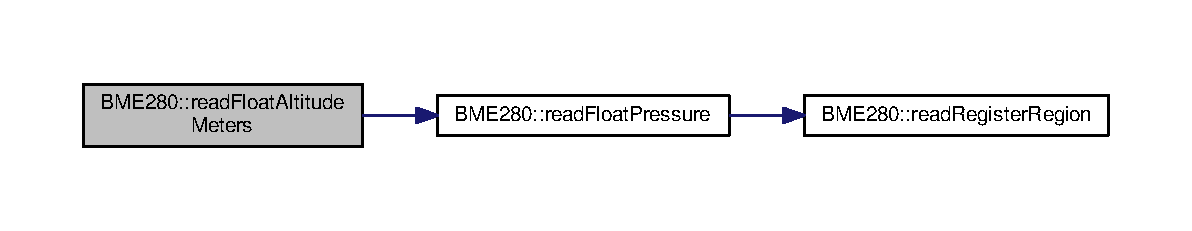
\includegraphics[width=350pt]{df/dcf/class_b_m_e280_af67b56ba50760ee1d116acc6c5010221_cgraph}
\end{center}
\end{figure}
Here is the caller graph for this function\+:\nopagebreak
\begin{figure}[H]
\begin{center}
\leavevmode
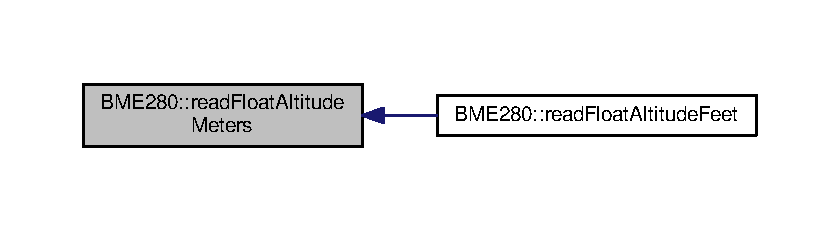
\includegraphics[width=350pt]{df/dcf/class_b_m_e280_af67b56ba50760ee1d116acc6c5010221_icgraph}
\end{center}
\end{figure}
\mbox{\Hypertarget{class_b_m_e280_a42ea7232039eebf5aadb391ef6132c35}\label{class_b_m_e280_a42ea7232039eebf5aadb391ef6132c35}} 
\index{B\+M\+E280@{B\+M\+E280}!read\+Float\+Humidity@{read\+Float\+Humidity}}
\index{read\+Float\+Humidity@{read\+Float\+Humidity}!B\+M\+E280@{B\+M\+E280}}
\subsubsection{\texorpdfstring{read\+Float\+Humidity()}{readFloatHumidity()}}
{\footnotesize\ttfamily float B\+M\+E280\+::read\+Float\+Humidity (\begin{DoxyParamCaption}\item[{void}]{ }\end{DoxyParamCaption})}



Definition at line 215 of file Cool\+Spark\+Fun\+B\+M\+E280.\+cpp.


\begin{DoxyCode}
216 \{
217     
218     \textcolor{comment}{// Returns humidity in %RH as unsigned 32 bit integer in Q22. 10 format (22 integer and 10 fractional
       bits).}
219     \textcolor{comment}{// Output value of “47445” represents 47445/1024 = 46. 333 %RH}
220     int32\_t adc\_H = ((uint32\_t)\hyperlink{class_b_m_e280_a1bbd14c8591966df531e40085342ff71}{readRegister}(\hyperlink{_cool_spark_fun_b_m_e280_8h_a463b030450826d7a286b272753c7c91c}{BME280\_HUMIDITY\_MSB\_REG}) << 
      8) | ((uint32\_t)\hyperlink{class_b_m_e280_a1bbd14c8591966df531e40085342ff71}{readRegister}(\hyperlink{_cool_spark_fun_b_m_e280_8h_a477dde6d1d96211aff748215ea9cd4dc}{BME280\_HUMIDITY\_LSB\_REG}));
221     
222     int32\_t var1;
223     var1 = (\hyperlink{class_b_m_e280_ad20f44914b78395f4d4bc64f4a68b369}{t\_fine} - ((int32\_t)76800));
224     var1 = (((((adc\_H << 14) - (((int32\_t)\hyperlink{class_b_m_e280_aa7a28484b6f5eb6f43261ea25016fbf8}{calibration}.\hyperlink{struct_sensor_calibration_a6b540f7bc56275b482d65e0725aeb27b}{dig\_H4}) << 20) - (((int32\_t)
      \hyperlink{class_b_m_e280_aa7a28484b6f5eb6f43261ea25016fbf8}{calibration}.\hyperlink{struct_sensor_calibration_a03691fc56b0bff17b007ffbd71dcc7b9}{dig\_H5}) * var1)) +
225     ((int32\_t)16384)) >> 15) * (((((((var1 * ((int32\_t)\hyperlink{class_b_m_e280_aa7a28484b6f5eb6f43261ea25016fbf8}{calibration}.
      \hyperlink{struct_sensor_calibration_a2f8c842c4becfce11e04c00168a9be0f}{dig\_H6})) >> 10) * (((var1 * ((int32\_t)\hyperlink{class_b_m_e280_aa7a28484b6f5eb6f43261ea25016fbf8}{calibration}.\hyperlink{struct_sensor_calibration_a65b525f9a3c58baf03db61da4626f417}{dig\_H3})) >> 11) + ((int32\_t)32768)
      )) >> 10) + ((int32\_t)2097152)) *
226     ((int32\_t)\hyperlink{class_b_m_e280_aa7a28484b6f5eb6f43261ea25016fbf8}{calibration}.\hyperlink{struct_sensor_calibration_afcfd149e907f83effaee0ae5dfa82a8f}{dig\_H2}) + 8192) >> 14));
227     var1 = (var1 - (((((var1 >> 15) * (var1 >> 15)) >> 7) * ((int32\_t)
      \hyperlink{class_b_m_e280_aa7a28484b6f5eb6f43261ea25016fbf8}{calibration}.\hyperlink{struct_sensor_calibration_ab8de0d58f5b0efa7ce638bed02deb460}{dig\_H1})) >> 4));
228     var1 = (var1 < 0 ? 0 : var1);
229     var1 = (var1 > 419430400 ? 419430400 : var1);
230 
231     \textcolor{keywordflow}{return} (\textcolor{keywordtype}{float})(var1>>12) / 1024.0;
232 
233 \}
\end{DoxyCode}
Here is the call graph for this function\+:\nopagebreak
\begin{figure}[H]
\begin{center}
\leavevmode
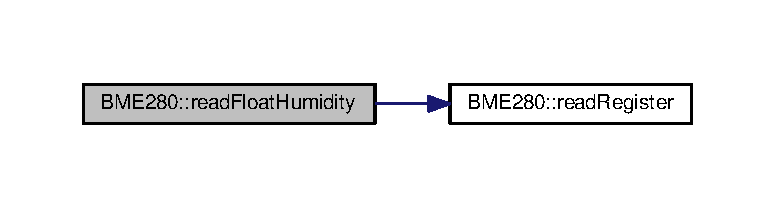
\includegraphics[width=350pt]{df/dcf/class_b_m_e280_a42ea7232039eebf5aadb391ef6132c35_cgraph}
\end{center}
\end{figure}
Here is the caller graph for this function\+:\nopagebreak
\begin{figure}[H]
\begin{center}
\leavevmode
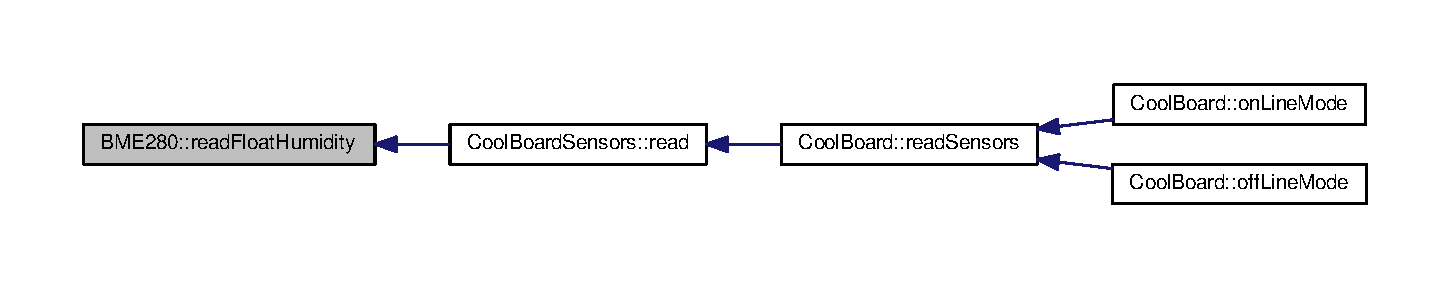
\includegraphics[width=350pt]{df/dcf/class_b_m_e280_a42ea7232039eebf5aadb391ef6132c35_icgraph}
\end{center}
\end{figure}
\mbox{\Hypertarget{class_b_m_e280_ada6e799917afb4f228e6253bc56ffe75}\label{class_b_m_e280_ada6e799917afb4f228e6253bc56ffe75}} 
\index{B\+M\+E280@{B\+M\+E280}!read\+Float\+Pressure@{read\+Float\+Pressure}}
\index{read\+Float\+Pressure@{read\+Float\+Pressure}!B\+M\+E280@{B\+M\+E280}}
\subsubsection{\texorpdfstring{read\+Float\+Pressure()}{readFloatPressure()}}
{\footnotesize\ttfamily float B\+M\+E280\+::read\+Float\+Pressure (\begin{DoxyParamCaption}\item[{void}]{ }\end{DoxyParamCaption})}



Definition at line 164 of file Cool\+Spark\+Fun\+B\+M\+E280.\+cpp.


\begin{DoxyCode}
165 \{
166 
167     \textcolor{comment}{// Returns pressure in Pa as unsigned 32 bit integer in Q24.8 format (24 integer bits and 8 fractional
       bits).}
168     \textcolor{comment}{// Output value of “24674867” represents 24674867/256 = 96386.2 Pa = 963.862 hPa}
169     int32\_t adc\_P = ((uint32\_t)\hyperlink{class_b_m_e280_a1bbd14c8591966df531e40085342ff71}{readRegister}(\hyperlink{_cool_spark_fun_b_m_e280_8h_ac60d376f920e64fe5855852658041c82}{BME280\_PRESSURE\_MSB\_REG}) << 
      12) | ((uint32\_t)\hyperlink{class_b_m_e280_a1bbd14c8591966df531e40085342ff71}{readRegister}(\hyperlink{_cool_spark_fun_b_m_e280_8h_acba4811c6b0815f807732a8c90cb1311}{BME280\_PRESSURE\_LSB\_REG}) << 4) | ((
      \hyperlink{class_b_m_e280_a1bbd14c8591966df531e40085342ff71}{readRegister}(\hyperlink{_cool_spark_fun_b_m_e280_8h_a76fa207f16ead1434519745ce83763e4}{BME280\_PRESSURE\_XLSB\_REG}) >> 4) & 0x0F);
170     
171     int64\_t var1, var2, p\_acc;
172     var1 = ((int64\_t)\hyperlink{class_b_m_e280_ad20f44914b78395f4d4bc64f4a68b369}{t\_fine}) - 128000;
173     var2 = var1 * var1 * (int64\_t)\hyperlink{class_b_m_e280_aa7a28484b6f5eb6f43261ea25016fbf8}{calibration}.\hyperlink{struct_sensor_calibration_ad1a973f775ee6d7f23d9197824971c76}{dig\_P6};
174     var2 = var2 + ((var1 * (int64\_t)\hyperlink{class_b_m_e280_aa7a28484b6f5eb6f43261ea25016fbf8}{calibration}.\hyperlink{struct_sensor_calibration_ae2508256bbfc0e222a677ebbd1d0acf7}{dig\_P5})<<17);
175     var2 = var2 + (((int64\_t)\hyperlink{class_b_m_e280_aa7a28484b6f5eb6f43261ea25016fbf8}{calibration}.\hyperlink{struct_sensor_calibration_a8af2a8c6f19a2a56e784aa9a7bd49cd3}{dig\_P4})<<35);
176     var1 = ((var1 * var1 * (int64\_t)\hyperlink{class_b_m_e280_aa7a28484b6f5eb6f43261ea25016fbf8}{calibration}.\hyperlink{struct_sensor_calibration_ac333ef210929de18815cec04c68acec2}{dig\_P3})>>8) + ((var1 * (int64\_t)
      \hyperlink{class_b_m_e280_aa7a28484b6f5eb6f43261ea25016fbf8}{calibration}.\hyperlink{struct_sensor_calibration_ab8a514b812ec77913dc95147d66bbcc4}{dig\_P2})<<12);
177     var1 = (((((int64\_t)1)<<47)+var1))*((int64\_t)\hyperlink{class_b_m_e280_aa7a28484b6f5eb6f43261ea25016fbf8}{calibration}.\hyperlink{struct_sensor_calibration_aba96e3c2bdbbe79c20a836d9c55c60cf}{dig\_P1})>>33;
178     \textcolor{keywordflow}{if} (var1 == 0)
179     \{
180         \textcolor{keywordflow}{return} 0; \textcolor{comment}{// avoid exception caused by division by zero}
181     \}
182     p\_acc = 1048576 - adc\_P;
183     p\_acc = (((p\_acc<<31) - var2)*3125)/var1;
184     var1 = (((int64\_t)\hyperlink{class_b_m_e280_aa7a28484b6f5eb6f43261ea25016fbf8}{calibration}.\hyperlink{struct_sensor_calibration_a5e942a51a1b5d7753719db1e27e55c06}{dig\_P9}) * (p\_acc>>13) * (p\_acc>>13)) >> 25;
185     var2 = (((int64\_t)\hyperlink{class_b_m_e280_aa7a28484b6f5eb6f43261ea25016fbf8}{calibration}.\hyperlink{struct_sensor_calibration_a06372d2918206f0cd35954e5bb35a1d2}{dig\_P8}) * p\_acc) >> 19;
186     p\_acc = ((p\_acc + var1 + var2) >> 8) + (((int64\_t)\hyperlink{class_b_m_e280_aa7a28484b6f5eb6f43261ea25016fbf8}{calibration}.
      \hyperlink{struct_sensor_calibration_adda4a99343f9e02de7d9f2d5949477d2}{dig\_P7})<<4);
187     
188     \textcolor{keywordflow}{return} (\textcolor{keywordtype}{float})p\_acc / 256.0;
189     
190 \}
\end{DoxyCode}
Here is the call graph for this function\+:\nopagebreak
\begin{figure}[H]
\begin{center}
\leavevmode
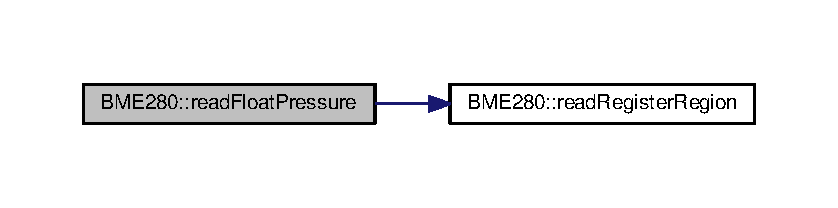
\includegraphics[width=350pt]{df/dcf/class_b_m_e280_ada6e799917afb4f228e6253bc56ffe75_cgraph}
\end{center}
\end{figure}
Here is the caller graph for this function\+:\nopagebreak
\begin{figure}[H]
\begin{center}
\leavevmode
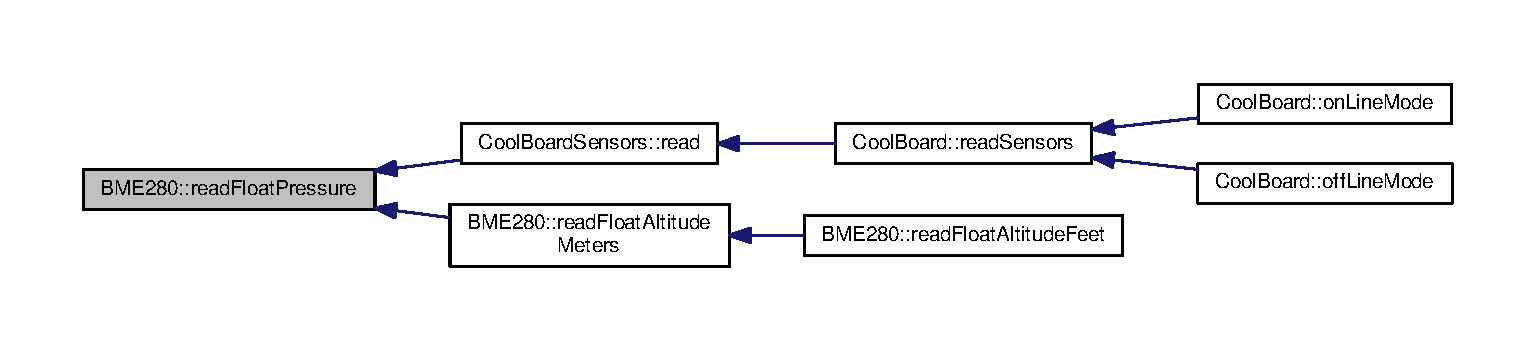
\includegraphics[width=350pt]{df/dcf/class_b_m_e280_ada6e799917afb4f228e6253bc56ffe75_icgraph}
\end{center}
\end{figure}
\mbox{\Hypertarget{class_b_m_e280_a1bbd14c8591966df531e40085342ff71}\label{class_b_m_e280_a1bbd14c8591966df531e40085342ff71}} 
\index{B\+M\+E280@{B\+M\+E280}!read\+Register@{read\+Register}}
\index{read\+Register@{read\+Register}!B\+M\+E280@{B\+M\+E280}}
\subsubsection{\texorpdfstring{read\+Register()}{readRegister()}}
{\footnotesize\ttfamily uint8\+\_\+t B\+M\+E280\+::read\+Register (\begin{DoxyParamCaption}\item[{uint8\+\_\+t}]{offset }\end{DoxyParamCaption})}



Definition at line 325 of file Cool\+Spark\+Fun\+B\+M\+E280.\+cpp.


\begin{DoxyCode}
326 \{
327     \textcolor{comment}{//Return value}
328     uint8\_t result;
329     uint8\_t numBytes = 1;
330     \textcolor{keywordflow}{switch} (\hyperlink{class_b_m_e280_af06253eb2f8ad4b5fabb858bc4a973bf}{settings}.\hyperlink{struct_sensor_settings_a5bf116387c543a6ea5732976424e8cb1}{commInterface}) \{
331 
332     \textcolor{keywordflow}{case} \hyperlink{_cool_spark_fun_b_m_e280_8h_a5cd01756030509b764d43a2b8c94fce8}{I2C\_MODE}:
333         Wire.beginTransmission(\hyperlink{class_b_m_e280_af06253eb2f8ad4b5fabb858bc4a973bf}{settings}.\hyperlink{struct_sensor_settings_af8103021dbce7e5ee6d786c4893324f7}{I2CAddress});
334         Wire.write(offset);
335         Wire.endTransmission();
336 
337         Wire.requestFrom(\hyperlink{class_b_m_e280_af06253eb2f8ad4b5fabb858bc4a973bf}{settings}.\hyperlink{struct_sensor_settings_af8103021dbce7e5ee6d786c4893324f7}{I2CAddress}, numBytes);
338         \textcolor{keywordflow}{while} ( Wire.available() ) \textcolor{comment}{// slave may send less than requested}
339         \{
340             result = Wire.read(); \textcolor{comment}{// receive a byte as a proper uint8\_t}
341         \}
342         \textcolor{keywordflow}{break};
343 
344     \textcolor{keywordflow}{case} \hyperlink{_cool_spark_fun_b_m_e280_8h_ab1dcc9464e3fcb94922386e8a7f53f21}{SPI\_MODE}:
345         \textcolor{comment}{// take the chip select low to select the device:}
346         digitalWrite(\hyperlink{class_b_m_e280_af06253eb2f8ad4b5fabb858bc4a973bf}{settings}.\hyperlink{struct_sensor_settings_abe2de606ebb580ad81e3fafb1a454580}{chipSelectPin}, LOW);
347         \textcolor{comment}{// send the device the register you want to read:}
348         SPI.transfer(offset | 0x80);  \textcolor{comment}{//Ored with "read request" bit}
349         \textcolor{comment}{// send a value of 0 to read the first byte returned:}
350         result = SPI.transfer(0x00);
351         \textcolor{comment}{// take the chip select high to de-select:}
352         digitalWrite(\hyperlink{class_b_m_e280_af06253eb2f8ad4b5fabb858bc4a973bf}{settings}.\hyperlink{struct_sensor_settings_abe2de606ebb580ad81e3fafb1a454580}{chipSelectPin}, HIGH);
353         \textcolor{keywordflow}{break};
354 
355     \textcolor{keywordflow}{default}:
356         \textcolor{keywordflow}{break};
357     \}
358     \textcolor{keywordflow}{return} result;
359 \}
\end{DoxyCode}
Here is the caller graph for this function\+:\nopagebreak
\begin{figure}[H]
\begin{center}
\leavevmode
\includegraphics[width=350pt]{df/dcf/class_b_m_e280_a1bbd14c8591966df531e40085342ff71_icgraph}
\end{center}
\end{figure}
\mbox{\Hypertarget{class_b_m_e280_ac43c30f9b321d301694094d6b4bebe7e}\label{class_b_m_e280_ac43c30f9b321d301694094d6b4bebe7e}} 
\index{B\+M\+E280@{B\+M\+E280}!read\+Register\+Int16@{read\+Register\+Int16}}
\index{read\+Register\+Int16@{read\+Register\+Int16}!B\+M\+E280@{B\+M\+E280}}
\subsubsection{\texorpdfstring{read\+Register\+Int16()}{readRegisterInt16()}}
{\footnotesize\ttfamily int16\+\_\+t B\+M\+E280\+::read\+Register\+Int16 (\begin{DoxyParamCaption}\item[{uint8\+\_\+t}]{offset }\end{DoxyParamCaption})}



Definition at line 361 of file Cool\+Spark\+Fun\+B\+M\+E280.\+cpp.


\begin{DoxyCode}
362 \{
363     uint8\_t myBuffer[2];
364     \hyperlink{class_b_m_e280_aecca87c2c40a7f2bcabcea921bdc6124}{readRegisterRegion}(myBuffer, offset, 2);  \textcolor{comment}{//Does memory transfer}
365     int16\_t output = (int16\_t)myBuffer[0] | int16\_t(myBuffer[1] << 8);
366     
367     \textcolor{keywordflow}{return} output;
368 \}
\end{DoxyCode}
Here is the call graph for this function\+:\nopagebreak
\begin{figure}[H]
\begin{center}
\leavevmode
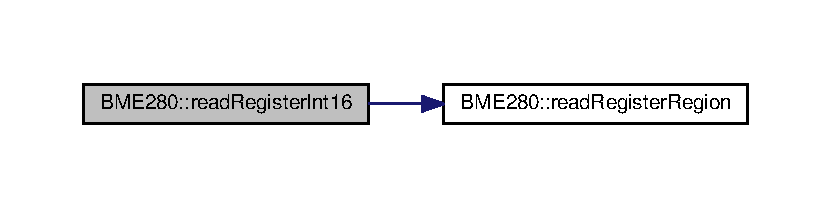
\includegraphics[width=350pt]{df/dcf/class_b_m_e280_ac43c30f9b321d301694094d6b4bebe7e_cgraph}
\end{center}
\end{figure}
\mbox{\Hypertarget{class_b_m_e280_aecca87c2c40a7f2bcabcea921bdc6124}\label{class_b_m_e280_aecca87c2c40a7f2bcabcea921bdc6124}} 
\index{B\+M\+E280@{B\+M\+E280}!read\+Register\+Region@{read\+Register\+Region}}
\index{read\+Register\+Region@{read\+Register\+Region}!B\+M\+E280@{B\+M\+E280}}
\subsubsection{\texorpdfstring{read\+Register\+Region()}{readRegisterRegion()}}
{\footnotesize\ttfamily void B\+M\+E280\+::read\+Register\+Region (\begin{DoxyParamCaption}\item[{uint8\+\_\+t $\ast$}]{output\+Pointer,  }\item[{uint8\+\_\+t}]{offset,  }\item[{uint8\+\_\+t}]{length }\end{DoxyParamCaption})}



Definition at line 278 of file Cool\+Spark\+Fun\+B\+M\+E280.\+cpp.


\begin{DoxyCode}
279 \{
280     \textcolor{comment}{//define pointer that will point to the external space}
281     uint8\_t i = 0;
282     \textcolor{keywordtype}{char} c = 0;
283 
284     \textcolor{keywordflow}{switch} (\hyperlink{class_b_m_e280_af06253eb2f8ad4b5fabb858bc4a973bf}{settings}.\hyperlink{struct_sensor_settings_a5bf116387c543a6ea5732976424e8cb1}{commInterface})
285     \{
286 
287     \textcolor{keywordflow}{case} \hyperlink{_cool_spark_fun_b_m_e280_8h_a5cd01756030509b764d43a2b8c94fce8}{I2C\_MODE}:
288         Wire.beginTransmission(\hyperlink{class_b_m_e280_af06253eb2f8ad4b5fabb858bc4a973bf}{settings}.\hyperlink{struct_sensor_settings_af8103021dbce7e5ee6d786c4893324f7}{I2CAddress});
289         Wire.write(offset);
290         Wire.endTransmission();
291 
292         \textcolor{comment}{// request bytes from slave device}
293         Wire.requestFrom(\hyperlink{class_b_m_e280_af06253eb2f8ad4b5fabb858bc4a973bf}{settings}.\hyperlink{struct_sensor_settings_af8103021dbce7e5ee6d786c4893324f7}{I2CAddress}, length);
294         \textcolor{keywordflow}{while} ( (Wire.available()) && (i < length))  \textcolor{comment}{// slave may send less than requested}
295         \{
296             c = Wire.read(); \textcolor{comment}{// receive a byte as character}
297             *outputPointer = c;
298             outputPointer++;
299             i++;
300         \}
301         \textcolor{keywordflow}{break};
302 
303     \textcolor{keywordflow}{case} \hyperlink{_cool_spark_fun_b_m_e280_8h_ab1dcc9464e3fcb94922386e8a7f53f21}{SPI\_MODE}:
304         \textcolor{comment}{// take the chip select low to select the device:}
305         digitalWrite(\hyperlink{class_b_m_e280_af06253eb2f8ad4b5fabb858bc4a973bf}{settings}.\hyperlink{struct_sensor_settings_abe2de606ebb580ad81e3fafb1a454580}{chipSelectPin}, LOW);
306         \textcolor{comment}{// send the device the register you want to read:}
307         SPI.transfer(offset | 0x80);  \textcolor{comment}{//Ored with "read request" bit}
308         \textcolor{keywordflow}{while} ( i < length ) \textcolor{comment}{// slave may send less than requested}
309         \{
310             c = SPI.transfer(0x00); \textcolor{comment}{// receive a byte as character}
311             *outputPointer = c;
312             outputPointer++;
313             i++;
314         \}
315         \textcolor{comment}{// take the chip select high to de-select:}
316         digitalWrite(\hyperlink{class_b_m_e280_af06253eb2f8ad4b5fabb858bc4a973bf}{settings}.\hyperlink{struct_sensor_settings_abe2de606ebb580ad81e3fafb1a454580}{chipSelectPin}, HIGH);
317         \textcolor{keywordflow}{break};
318 
319     \textcolor{keywordflow}{default}:
320         \textcolor{keywordflow}{break};
321     \}
322 
323 \}
\end{DoxyCode}
Here is the caller graph for this function\+:\nopagebreak
\begin{figure}[H]
\begin{center}
\leavevmode
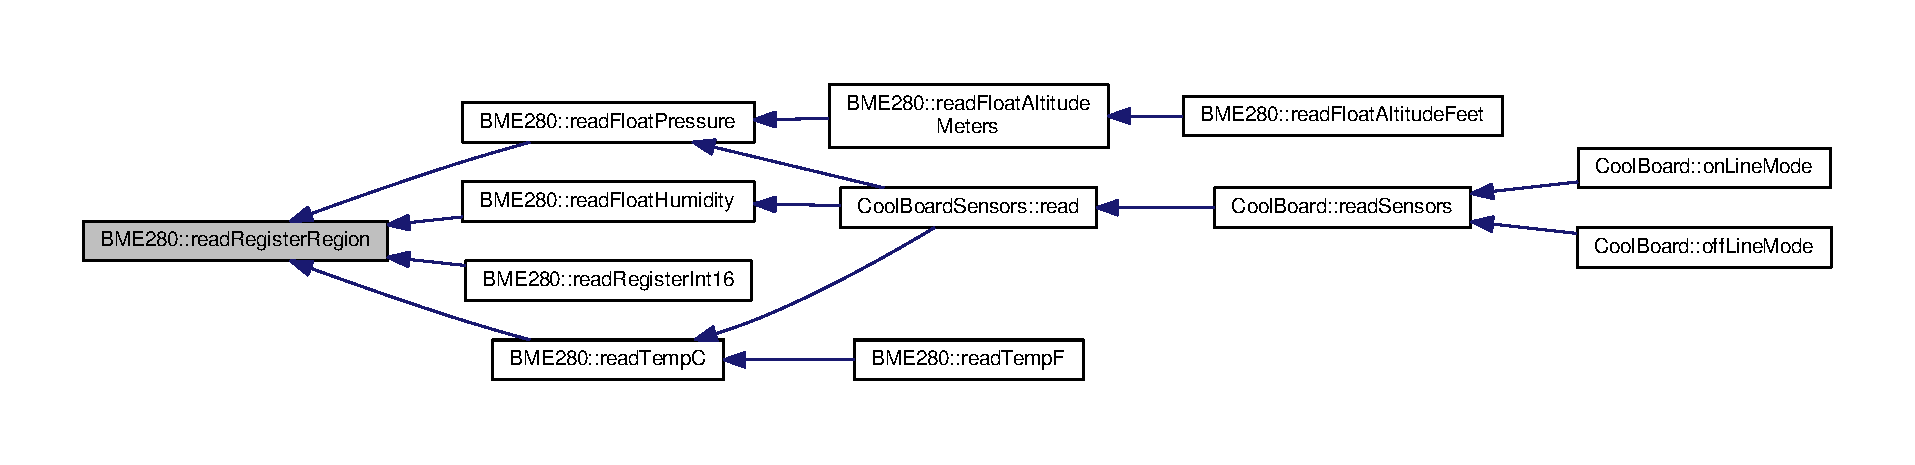
\includegraphics[width=350pt]{df/dcf/class_b_m_e280_aecca87c2c40a7f2bcabcea921bdc6124_icgraph}
\end{center}
\end{figure}
\mbox{\Hypertarget{class_b_m_e280_afffdd1d7ded9e1f92200e70669019d97}\label{class_b_m_e280_afffdd1d7ded9e1f92200e70669019d97}} 
\index{B\+M\+E280@{B\+M\+E280}!read\+TempC@{read\+TempC}}
\index{read\+TempC@{read\+TempC}!B\+M\+E280@{B\+M\+E280}}
\subsubsection{\texorpdfstring{read\+Temp\+C()}{readTempC()}}
{\footnotesize\ttfamily float B\+M\+E280\+::read\+TempC (\begin{DoxyParamCaption}\item[{void}]{ }\end{DoxyParamCaption})}



Definition at line 243 of file Cool\+Spark\+Fun\+B\+M\+E280.\+cpp.


\begin{DoxyCode}
244 \{
245     \textcolor{comment}{// Returns temperature in DegC, resolution is 0.01 DegC. Output value of “5123” equals 51.23 DegC.}
246     \textcolor{comment}{// t\_fine carries fine temperature as global value}
247 
248     \textcolor{comment}{//get the reading (adc\_T);}
249     int32\_t adc\_T = ((uint32\_t)\hyperlink{class_b_m_e280_a1bbd14c8591966df531e40085342ff71}{readRegister}(
      \hyperlink{_cool_spark_fun_b_m_e280_8h_a274a08bbc75e1b359aa6c46b50954b33}{BME280\_TEMPERATURE\_MSB\_REG}) << 12) | ((uint32\_t)
      \hyperlink{class_b_m_e280_a1bbd14c8591966df531e40085342ff71}{readRegister}(\hyperlink{_cool_spark_fun_b_m_e280_8h_ab54b428fbb78e70606ce994fcbfbc6aa}{BME280\_TEMPERATURE\_LSB\_REG}) << 4) | ((
      \hyperlink{class_b_m_e280_a1bbd14c8591966df531e40085342ff71}{readRegister}(\hyperlink{_cool_spark_fun_b_m_e280_8h_a1376db91beb753a83dbbd8f1d0716a56}{BME280\_TEMPERATURE\_XLSB\_REG}) >> 4) & 0x0F);
250 
251     \textcolor{comment}{//By datasheet, calibrate}
252     int64\_t var1, var2;
253 
254     var1 = ((((adc\_T>>3) - ((int32\_t)\hyperlink{class_b_m_e280_aa7a28484b6f5eb6f43261ea25016fbf8}{calibration}.\hyperlink{struct_sensor_calibration_a044a8c40e958b1cda3fb85b95303550e}{dig\_T1}<<1))) * ((int32\_t)
      \hyperlink{class_b_m_e280_aa7a28484b6f5eb6f43261ea25016fbf8}{calibration}.\hyperlink{struct_sensor_calibration_a8f8bb62e10c9bc0decb4463128ccaee5}{dig\_T2})) >> 11;
255     var2 = (((((adc\_T>>4) - ((int32\_t)\hyperlink{class_b_m_e280_aa7a28484b6f5eb6f43261ea25016fbf8}{calibration}.\hyperlink{struct_sensor_calibration_a044a8c40e958b1cda3fb85b95303550e}{dig\_T1})) * ((adc\_T>>4) - ((int32\_t)
      \hyperlink{class_b_m_e280_aa7a28484b6f5eb6f43261ea25016fbf8}{calibration}.\hyperlink{struct_sensor_calibration_a044a8c40e958b1cda3fb85b95303550e}{dig\_T1}))) >> 12) *
256     ((int32\_t)\hyperlink{class_b_m_e280_aa7a28484b6f5eb6f43261ea25016fbf8}{calibration}.\hyperlink{struct_sensor_calibration_a5b134db1776888487855c6b526d130d6}{dig\_T3})) >> 14;
257     \hyperlink{class_b_m_e280_ad20f44914b78395f4d4bc64f4a68b369}{t\_fine} = var1 + var2;
258     \textcolor{keywordtype}{float} output = (\hyperlink{class_b_m_e280_ad20f44914b78395f4d4bc64f4a68b369}{t\_fine} * 5 + 128) >> 8;
259 
260     output = output / 100;
261     
262     \textcolor{keywordflow}{return} output;
263 \}
\end{DoxyCode}
Here is the call graph for this function\+:\nopagebreak
\begin{figure}[H]
\begin{center}
\leavevmode
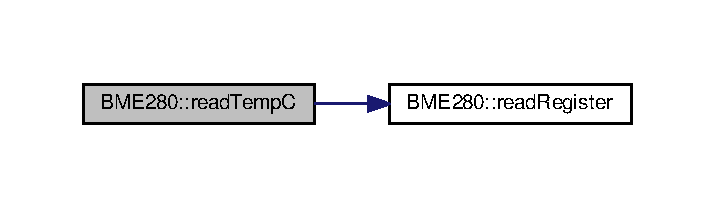
\includegraphics[width=343pt]{df/dcf/class_b_m_e280_afffdd1d7ded9e1f92200e70669019d97_cgraph}
\end{center}
\end{figure}
Here is the caller graph for this function\+:\nopagebreak
\begin{figure}[H]
\begin{center}
\leavevmode
\includegraphics[width=350pt]{df/dcf/class_b_m_e280_afffdd1d7ded9e1f92200e70669019d97_icgraph}
\end{center}
\end{figure}
\mbox{\Hypertarget{class_b_m_e280_a9648b496f6b4700550782a715a98b3c7}\label{class_b_m_e280_a9648b496f6b4700550782a715a98b3c7}} 
\index{B\+M\+E280@{B\+M\+E280}!read\+TempF@{read\+TempF}}
\index{read\+TempF@{read\+TempF}!B\+M\+E280@{B\+M\+E280}}
\subsubsection{\texorpdfstring{read\+Temp\+F()}{readTempF()}}
{\footnotesize\ttfamily float B\+M\+E280\+::read\+TempF (\begin{DoxyParamCaption}\item[{void}]{ }\end{DoxyParamCaption})}



Definition at line 265 of file Cool\+Spark\+Fun\+B\+M\+E280.\+cpp.


\begin{DoxyCode}
266 \{
267     \textcolor{keywordtype}{float} output = \hyperlink{class_b_m_e280_afffdd1d7ded9e1f92200e70669019d97}{readTempC}();
268     output = (output * 9) / 5 + 32;
269 
270     \textcolor{keywordflow}{return} output;
271 \}
\end{DoxyCode}
Here is the call graph for this function\+:\nopagebreak
\begin{figure}[H]
\begin{center}
\leavevmode
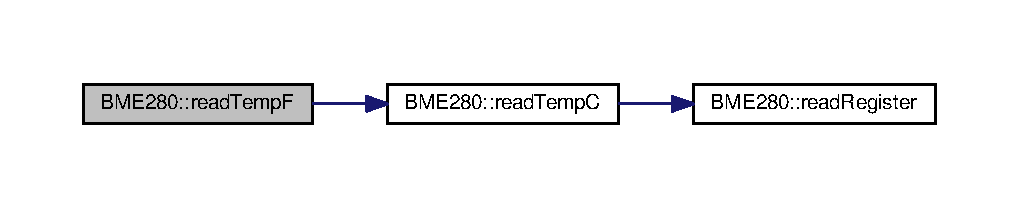
\includegraphics[width=350pt]{df/dcf/class_b_m_e280_a9648b496f6b4700550782a715a98b3c7_cgraph}
\end{center}
\end{figure}
\mbox{\Hypertarget{class_b_m_e280_aeec5deb6daace6ae390108b4210e9df7}\label{class_b_m_e280_aeec5deb6daace6ae390108b4210e9df7}} 
\index{B\+M\+E280@{B\+M\+E280}!reset@{reset}}
\index{reset@{reset}!B\+M\+E280@{B\+M\+E280}}
\subsubsection{\texorpdfstring{reset()}{reset()}}
{\footnotesize\ttfamily void B\+M\+E280\+::reset (\begin{DoxyParamCaption}\item[{void}]{ }\end{DoxyParamCaption})}



Definition at line 153 of file Cool\+Spark\+Fun\+B\+M\+E280.\+cpp.


\begin{DoxyCode}
154 \{
155     \hyperlink{class_b_m_e280_afcff21c342725246bf415d7f0e4d04f0}{writeRegister}(\hyperlink{_cool_spark_fun_b_m_e280_8h_a58ebcaa8ff137ca7e8704dbfb70dff57}{BME280\_RST\_REG}, 0xB6);
156     
157 \}
\end{DoxyCode}
Here is the call graph for this function\+:\nopagebreak
\begin{figure}[H]
\begin{center}
\leavevmode
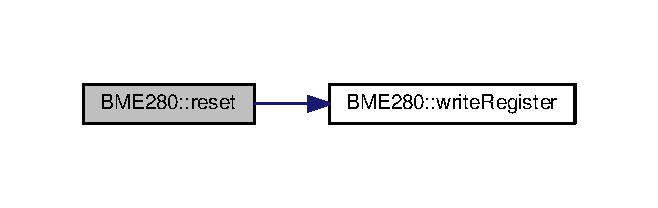
\includegraphics[width=316pt]{df/dcf/class_b_m_e280_aeec5deb6daace6ae390108b4210e9df7_cgraph}
\end{center}
\end{figure}
\mbox{\Hypertarget{class_b_m_e280_afcff21c342725246bf415d7f0e4d04f0}\label{class_b_m_e280_afcff21c342725246bf415d7f0e4d04f0}} 
\index{B\+M\+E280@{B\+M\+E280}!write\+Register@{write\+Register}}
\index{write\+Register@{write\+Register}!B\+M\+E280@{B\+M\+E280}}
\subsubsection{\texorpdfstring{write\+Register()}{writeRegister()}}
{\footnotesize\ttfamily void B\+M\+E280\+::write\+Register (\begin{DoxyParamCaption}\item[{uint8\+\_\+t}]{offset,  }\item[{uint8\+\_\+t}]{data\+To\+Write }\end{DoxyParamCaption})}



Definition at line 370 of file Cool\+Spark\+Fun\+B\+M\+E280.\+cpp.


\begin{DoxyCode}
371 \{
372     \textcolor{keywordflow}{switch} (\hyperlink{class_b_m_e280_af06253eb2f8ad4b5fabb858bc4a973bf}{settings}.\hyperlink{struct_sensor_settings_a5bf116387c543a6ea5732976424e8cb1}{commInterface})
373     \{
374     \textcolor{keywordflow}{case} \hyperlink{_cool_spark_fun_b_m_e280_8h_a5cd01756030509b764d43a2b8c94fce8}{I2C\_MODE}:
375         \textcolor{comment}{//Write the byte}
376         Wire.beginTransmission(\hyperlink{class_b_m_e280_af06253eb2f8ad4b5fabb858bc4a973bf}{settings}.\hyperlink{struct_sensor_settings_af8103021dbce7e5ee6d786c4893324f7}{I2CAddress});
377         Wire.write(offset);
378         Wire.write(dataToWrite);
379         Wire.endTransmission();
380         \textcolor{keywordflow}{break};
381 
382     \textcolor{keywordflow}{case} \hyperlink{_cool_spark_fun_b_m_e280_8h_ab1dcc9464e3fcb94922386e8a7f53f21}{SPI\_MODE}:
383         \textcolor{comment}{// take the chip select low to select the device:}
384         digitalWrite(\hyperlink{class_b_m_e280_af06253eb2f8ad4b5fabb858bc4a973bf}{settings}.\hyperlink{struct_sensor_settings_abe2de606ebb580ad81e3fafb1a454580}{chipSelectPin}, LOW);
385         \textcolor{comment}{// send the device the register you want to read:}
386         SPI.transfer(offset & 0x7F);
387         \textcolor{comment}{// send a value of 0 to read the first byte returned:}
388         SPI.transfer(dataToWrite);
389         \textcolor{comment}{// decrement the number of bytes left to read:}
390         \textcolor{comment}{// take the chip select high to de-select:}
391         digitalWrite(\hyperlink{class_b_m_e280_af06253eb2f8ad4b5fabb858bc4a973bf}{settings}.\hyperlink{struct_sensor_settings_abe2de606ebb580ad81e3fafb1a454580}{chipSelectPin}, HIGH);
392         \textcolor{keywordflow}{break};
393 
394     \textcolor{keywordflow}{default}:
395         \textcolor{keywordflow}{break};
396     \}
397 \}
\end{DoxyCode}
Here is the caller graph for this function\+:\nopagebreak
\begin{figure}[H]
\begin{center}
\leavevmode
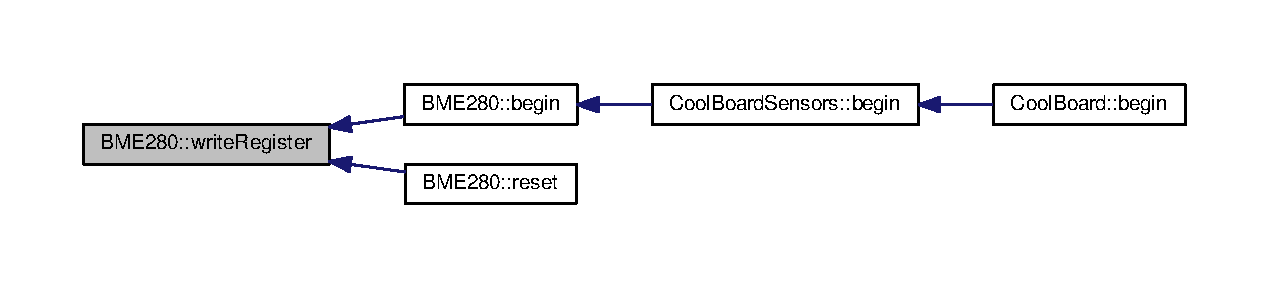
\includegraphics[width=350pt]{df/dcf/class_b_m_e280_afcff21c342725246bf415d7f0e4d04f0_icgraph}
\end{center}
\end{figure}


\subsection{Member Data Documentation}
\mbox{\Hypertarget{class_b_m_e280_aa7a28484b6f5eb6f43261ea25016fbf8}\label{class_b_m_e280_aa7a28484b6f5eb6f43261ea25016fbf8}} 
\index{B\+M\+E280@{B\+M\+E280}!calibration@{calibration}}
\index{calibration@{calibration}!B\+M\+E280@{B\+M\+E280}}
\subsubsection{\texorpdfstring{calibration}{calibration}}
{\footnotesize\ttfamily \hyperlink{struct_sensor_calibration}{Sensor\+Calibration} B\+M\+E280\+::calibration}



Definition at line 148 of file Cool\+Spark\+Fun\+B\+M\+E280.\+h.

\mbox{\Hypertarget{class_b_m_e280_af06253eb2f8ad4b5fabb858bc4a973bf}\label{class_b_m_e280_af06253eb2f8ad4b5fabb858bc4a973bf}} 
\index{B\+M\+E280@{B\+M\+E280}!settings@{settings}}
\index{settings@{settings}!B\+M\+E280@{B\+M\+E280}}
\subsubsection{\texorpdfstring{settings}{settings}}
{\footnotesize\ttfamily \hyperlink{struct_sensor_settings}{Sensor\+Settings} B\+M\+E280\+::settings}



Definition at line 147 of file Cool\+Spark\+Fun\+B\+M\+E280.\+h.

\mbox{\Hypertarget{class_b_m_e280_ad20f44914b78395f4d4bc64f4a68b369}\label{class_b_m_e280_ad20f44914b78395f4d4bc64f4a68b369}} 
\index{B\+M\+E280@{B\+M\+E280}!t\+\_\+fine@{t\+\_\+fine}}
\index{t\+\_\+fine@{t\+\_\+fine}!B\+M\+E280@{B\+M\+E280}}
\subsubsection{\texorpdfstring{t\+\_\+fine}{t\_fine}}
{\footnotesize\ttfamily int32\+\_\+t B\+M\+E280\+::t\+\_\+fine}



Definition at line 149 of file Cool\+Spark\+Fun\+B\+M\+E280.\+h.



The documentation for this class was generated from the following files\+:\begin{DoxyCompactItemize}
\item 
/home/ashiroji/\+Arduino/libraries/\+Cool\+Board/src/internals/\hyperlink{_cool_spark_fun_b_m_e280_8h}{Cool\+Spark\+Fun\+B\+M\+E280.\+h}\item 
/home/ashiroji/\+Arduino/libraries/\+Cool\+Board/src/internals/\hyperlink{_cool_spark_fun_b_m_e280_8cpp}{Cool\+Spark\+Fun\+B\+M\+E280.\+cpp}\end{DoxyCompactItemize}

\hypertarget{class_cool_board}{}\section{Cool\+Board Class Reference}
\label{class_cool_board}\index{Cool\+Board@{Cool\+Board}}


This class manages the \hyperlink{class_cool_board}{Cool\+Board} and all of Its functions.  




{\ttfamily \#include $<$Cool\+Board.\+h$>$}



Collaboration diagram for Cool\+Board\+:
\nopagebreak
\begin{figure}[H]
\begin{center}
\leavevmode
\includegraphics[width=350pt]{d5/d3a/class_cool_board__coll__graph}
\end{center}
\end{figure}
\subsection*{Public Member Functions}
\begin{DoxyCompactItemize}
\item 
\hyperlink{class_cool_board_a8b88fd781e22e93025dd63474113b7e4}{Cool\+Board} ()
\item 
void \hyperlink{class_cool_board_acba7c5aef7268b2c0044bdb54d3b9d76}{begin} ()
\item 
bool \hyperlink{class_cool_board_a583a874c09c07e70a6eb9229fc4beddb}{config} ()
\item 
void \hyperlink{class_cool_board_a8612756d3f73198cdde857a66f0fe690}{update} (const char $\ast$\hyperlink{class_cool_board_a7b835fafd449e5282f7f91d787a2dc15}{answer})
\item 
void \hyperlink{class_cool_board_ae6b5e1274d760462290192acea4adca8}{off\+Line\+Mode} ()
\item 
void \hyperlink{class_cool_board_aa0bbc4bc605e35618d18e68795c61363}{on\+Line\+Mode} ()
\item 
int \hyperlink{class_cool_board_a519de78b807f8ec6463ff484eb925918}{connect} ()
\item 
int \hyperlink{class_cool_board_ad7442cf4b62c7b0d5bd62a0f75ffc065}{is\+Connected} ()
\item 
unsigned long \hyperlink{class_cool_board_a7508e029f2ee17bb747ffab599285e0d}{get\+Log\+Interval} ()
\item 
void \hyperlink{class_cool_board_a486507b8f0981d3cc671ed31c2145755}{print\+Conf} ()
\item 
void \hyperlink{class_cool_board_a069952cdcb2e7f68518aa429eceadb6e}{sleep} (unsigned long interval)
\item 
String \hyperlink{class_cool_board_ad03abdce2e65f520bbf2cff0f2d083cf}{read\+Sensors} ()
\item 
void \hyperlink{class_cool_board_a397b46fadab8f530a8cf4d914c561366}{init\+Read\+I2C} ()
\item 
String \hyperlink{class_cool_board_ae7358fb6e623cfc81b775f5f1734909b}{user\+Data} ()
\end{DoxyCompactItemize}
\subsection*{Private Attributes}
\begin{DoxyCompactItemize}
\item 
\hyperlink{class_cool_file_system}{Cool\+File\+System} \hyperlink{class_cool_board_a42c2586fbb13ff7f06538e9284e8538d}{file\+System}
\item 
\hyperlink{class_cool_board_sensors}{Cool\+Board\+Sensors} \hyperlink{class_cool_board_af102be5288bd7f7a8e59b13f86e26a00}{cool\+Board\+Sensors}
\item 
\hyperlink{class_cool_board_led}{Cool\+Board\+Led} \hyperlink{class_cool_board_a1b1d3c684a5baa56b08486e192fd8e97}{cool\+Board\+Led}
\item 
\hyperlink{class_cool_time}{Cool\+Time} \hyperlink{class_cool_board_a50d2a6716879d64a85f3c6b44ad63275}{rtc}
\item 
\hyperlink{class_cool_wifi}{Cool\+Wifi} \hyperlink{class_cool_board_acd88e6003606b47479ebba81e4aceeca}{wifi\+Manager}
\item 
\hyperlink{class_cool_m_q_t_t}{Cool\+M\+Q\+TT} \hyperlink{class_cool_board_a2399f44d7c23c1149a335cb3b46d90f1}{mqtt}
\item 
\hyperlink{class_jetpack}{Jetpack} \hyperlink{class_cool_board_a30b1357881b01ccbec676856a91e48e9}{jet\+Pack}
\item 
\hyperlink{class_irene3000}{Irene3000} \hyperlink{class_cool_board_ad103718ce316006c4695b8eb312eaf11}{irene3000}
\item 
\hyperlink{class_external_sensors}{External\+Sensors} \hyperlink{class_cool_board_a09e26264839c65873eb56af476eff6b2}{external\+Sensors}
\item 
\hyperlink{class_cool_board_actor}{Cool\+Board\+Actor} \hyperlink{class_cool_board_a4ac693895c21025b8808653f2a4316e6}{on\+Board\+Actor}
\item 
bool \hyperlink{class_cool_board_a6395459131d6889a3005f79c7a35e964}{user\+Active} =0
\item 
bool \hyperlink{class_cool_board_a9c3f7ac625481ee2ae802a25d97a4ae0}{irene\+Active} =0
\item 
bool \hyperlink{class_cool_board_a9be03a913d26e558328935ca3b59a75e}{jetpack\+Active} =0
\item 
bool \hyperlink{class_cool_board_a638b00b76aeb819ecfd4c10b8cdd7bb7}{external\+Sensors\+Active} =0
\item 
bool \hyperlink{class_cool_board_a0a51b2287139f66c738101fb53139230}{sleep\+Active} =0
\item 
bool \hyperlink{class_cool_board_a7c8e505a5804b109e112d5a03df6ea2b}{manual} =0
\item 
unsigned long \hyperlink{class_cool_board_a84bc94413b64973e4aba8c467c97006c}{log\+Interval} =1
\item 
String \hyperlink{class_cool_board_a427fb753dd8575bdf821c70a5c63d695}{data} =\char`\"{}\char`\"{}
\item 
String \hyperlink{class_cool_board_a7b835fafd449e5282f7f91d787a2dc15}{answer} =\char`\"{}\char`\"{}
\item 
const int \hyperlink{class_cool_board_af1fe1376fc66f93dee80b327ca695377}{En\+I2C} = 5
\end{DoxyCompactItemize}


\subsection{Detailed Description}
This class manages the \hyperlink{class_cool_board}{Cool\+Board} and all of Its functions. 

Definition at line 34 of file Cool\+Board.\+h.



\subsection{Constructor \& Destructor Documentation}
\mbox{\Hypertarget{class_cool_board_a8b88fd781e22e93025dd63474113b7e4}\label{class_cool_board_a8b88fd781e22e93025dd63474113b7e4}} 
\index{Cool\+Board@{Cool\+Board}!Cool\+Board@{Cool\+Board}}
\index{Cool\+Board@{Cool\+Board}!Cool\+Board@{Cool\+Board}}
\subsubsection{\texorpdfstring{Cool\+Board()}{CoolBoard()}}
{\footnotesize\ttfamily Cool\+Board\+::\+Cool\+Board (\begin{DoxyParamCaption}{ }\end{DoxyParamCaption})}

\hyperlink{class_cool_board_a8b88fd781e22e93025dd63474113b7e4}{Cool\+Board\+::\+Cool\+Board()}\+: This Constructor is provided to start the I2C interface and Init the different used pins 

Definition at line 28 of file Cool\+Board.\+cpp.


\begin{DoxyCode}
29 \{
30 
31 \textcolor{preprocessor}{#if DEBUG == 1}
32 
33     Serial.println( F(\textcolor{stringliteral}{"Entering CoolBoard Constructor"}) );
34     Serial.println();
35 
36 \textcolor{preprocessor}{#endif}
37     
38     Wire.begin(2, 14);                       \textcolor{comment}{//I2C init }
39 
40     pinMode(\hyperlink{class_cool_board_af1fe1376fc66f93dee80b327ca695377}{EnI2C}, OUTPUT);           \textcolor{comment}{//Declare I2C Enable pin }
41 
42 \}
\end{DoxyCode}


\subsection{Member Function Documentation}
\mbox{\Hypertarget{class_cool_board_acba7c5aef7268b2c0044bdb54d3b9d76}\label{class_cool_board_acba7c5aef7268b2c0044bdb54d3b9d76}} 
\index{Cool\+Board@{Cool\+Board}!begin@{begin}}
\index{begin@{begin}!Cool\+Board@{Cool\+Board}}
\subsubsection{\texorpdfstring{begin()}{begin()}}
{\footnotesize\ttfamily void Cool\+Board\+::begin (\begin{DoxyParamCaption}{ }\end{DoxyParamCaption})}

\hyperlink{class_cool_board_acba7c5aef7268b2c0044bdb54d3b9d76}{Cool\+Board\+::begin()}\+: This method is provided to configure and start the used Cool\+Kit Parts. It also starts the first connection try If Serial is enabled,it prints the configuration of the used parts. 

Definition at line 53 of file Cool\+Board.\+cpp.


\begin{DoxyCode}
54 \{
55 
56 \textcolor{preprocessor}{#if DEBUG == 1}
57 
58     Serial.println( F(\textcolor{stringliteral}{"Starting the CoolBoard  "})  );
59     Serial.println( F(\textcolor{stringliteral}{"Entering CoolBoard.begin() "})  );
60     Serial.println();
61 \textcolor{preprocessor}{#endif  }
62 
63 \textcolor{preprocessor}{#if DEBUG == 0}
64     Serial.println( F(\textcolor{stringliteral}{"Starting Coolboard..."}));
65 \textcolor{preprocessor}{#endif}
66 
67 
68     delay(100);
69     
70     \hyperlink{class_cool_board_a1b1d3c684a5baa56b08486e192fd8e97}{coolBoardLed}.\hyperlink{class_cool_board_led_a30fadd4cbec17ceea428bf7a32207e87}{write}(255,128,0);\textcolor{comment}{//orange}
71 
72     this->\hyperlink{class_cool_board_a397b46fadab8f530a8cf4d914c561366}{initReadI2C}();
73     delay(50);
74 
75     \hyperlink{class_cool_board_af102be5288bd7f7a8e59b13f86e26a00}{coolBoardSensors}.\hyperlink{class_cool_board_sensors_a9a218895c5423375c33c08f2c56fb23a}{config}();
76     \hyperlink{class_cool_board_af102be5288bd7f7a8e59b13f86e26a00}{coolBoardSensors}.\hyperlink{class_cool_board_sensors_a97095823ef7c8f5290812f1405b966b3}{begin}();
77     delay(100);
78     
79     \hyperlink{class_cool_board_a4ac693895c21025b8808653f2a4316e6}{onBoardActor}.\hyperlink{class_cool_board_actor_a5af5538fc7d169f63127e06d5219bcd4}{config}();
80     \hyperlink{class_cool_board_a4ac693895c21025b8808653f2a4316e6}{onBoardActor}.\hyperlink{class_cool_board_actor_a7f4422fd85a5510bc2cdfd68e109be5e}{begin}();
81     delay(100);
82     
83     \hyperlink{class_cool_board_acd88e6003606b47479ebba81e4aceeca}{wifiManager}.\hyperlink{class_cool_wifi_a4eb2f6b9b09dd588964b88b6c70122c0}{config}();
84     \hyperlink{class_cool_board_acd88e6003606b47479ebba81e4aceeca}{wifiManager}.\hyperlink{class_cool_wifi_a46942fed90e475112cc10b78a32e7aaa}{begin}();
85     delay(100);
86 
87     \hyperlink{class_cool_board_a2399f44d7c23c1149a335cb3b46d90f1}{mqtt}.\hyperlink{class_cool_m_q_t_t_a9b703de4f1358f0ee7a5e8c44979c648}{config}();
88     \hyperlink{class_cool_board_a2399f44d7c23c1149a335cb3b46d90f1}{mqtt}.\hyperlink{class_cool_m_q_t_t_ac9248808641ebf3054ed0620ea9d0100}{begin}();
89     delay(100);
90 
91 \textcolor{preprocessor}{#if DEBUG == 1}
92 
93     \hyperlink{class_cool_board_a1b1d3c684a5baa56b08486e192fd8e97}{coolBoardLed}.\hyperlink{class_cool_board_led_a8ed3053a36f0ed4a131f43b5b17efb61}{printConf}();
94 
95     \hyperlink{class_cool_board_af102be5288bd7f7a8e59b13f86e26a00}{coolBoardSensors}.\hyperlink{class_cool_board_sensors_af6fd79505815b204c178617ecf54c873}{printConf}();
96 
97     \hyperlink{class_cool_board_a4ac693895c21025b8808653f2a4316e6}{onBoardActor}.\hyperlink{class_cool_board_actor_aabb10e7aebc3249ffc940530de29f84a}{printConf}();
98 
99     \hyperlink{class_cool_board_acd88e6003606b47479ebba81e4aceeca}{wifiManager}.\hyperlink{class_cool_wifi_a9e6105c6d13d35ec510f6633da9e0223}{printConf}();
100 
101     \hyperlink{class_cool_board_a2399f44d7c23c1149a335cb3b46d90f1}{mqtt}.\hyperlink{class_cool_m_q_t_t_a40553a0ad4b5ecf1cb4411ab54ca85fb}{printConf}();
102     
103 
104 \textcolor{preprocessor}{#endif}
105 
106 
107     \textcolor{keywordflow}{if} (\hyperlink{class_cool_board_a9be03a913d26e558328935ca3b59a75e}{jetpackActive})
108     \{
109         \hyperlink{class_cool_board_a30b1357881b01ccbec676856a91e48e9}{jetPack}.\hyperlink{class_jetpack_ab065ee83e244265a2223a22f3ee4a719}{config}();
110         \hyperlink{class_cool_board_a30b1357881b01ccbec676856a91e48e9}{jetPack}.\hyperlink{class_jetpack_a5a53e1ebf7aaf3bf3e0d37ea64ca09a7}{begin}();
111 
112 \textcolor{preprocessor}{    #if DEBUG == 1}
113         
114         \hyperlink{class_cool_board_a30b1357881b01ccbec676856a91e48e9}{jetPack}.\hyperlink{class_jetpack_ac54a7bb4f9166bee32052253d9b1d306}{printConf}();
115 
116 \textcolor{preprocessor}{    #endif}
117         delay(100);
118     \}
119 
120     \textcolor{keywordflow}{if} (\hyperlink{class_cool_board_a9c3f7ac625481ee2ae802a25d97a4ae0}{ireneActive})
121     \{
122         \hyperlink{class_cool_board_ad103718ce316006c4695b8eb312eaf11}{irene3000}.\hyperlink{class_irene3000_afed5c35e4b23963c157847ef27c11e9c}{config}();
123         \hyperlink{class_cool_board_ad103718ce316006c4695b8eb312eaf11}{irene3000}.\hyperlink{class_irene3000_ad5891806c500ae1007afe52b9e304c2b}{begin}();
124 
125 \textcolor{preprocessor}{    #if DEBUG == 1}
126 
127         \hyperlink{class_cool_board_ad103718ce316006c4695b8eb312eaf11}{irene3000}.\hyperlink{class_irene3000_a7bc2414100b5e19eacc6630fa34b2654}{printConf}();
128 
129 \textcolor{preprocessor}{    #endif}
130         delay(100);
131     \}
132 
133     \textcolor{keywordflow}{if} (\hyperlink{class_cool_board_a638b00b76aeb819ecfd4c10b8cdd7bb7}{externalSensorsActive})
134     \{
135         \hyperlink{class_cool_board_a09e26264839c65873eb56af476eff6b2}{externalSensors}.\hyperlink{class_external_sensors_a862a4bd11346b37270d0244c2adabe5a}{config}();
136         \hyperlink{class_cool_board_a09e26264839c65873eb56af476eff6b2}{externalSensors}.\hyperlink{class_external_sensors_a58ede0d786a86417254708870f04a21e}{begin}();
137 
138 \textcolor{preprocessor}{    #if DEBUG == 1}
139 
140         \hyperlink{class_cool_board_a09e26264839c65873eb56af476eff6b2}{externalSensors}.\hyperlink{class_external_sensors_a78c2bf55084435dd51d3c559b2d3c6f3}{printConf}();
141 
142 \textcolor{preprocessor}{    #endif}
143         delay(100);
144     \}
145     
146     \hyperlink{class_cool_board_a1b1d3c684a5baa56b08486e192fd8e97}{coolBoardLed}.\hyperlink{class_cool_board_led_a93d545679237e8cc858324367149775c}{fadeOut}(255,128,0,0.5);\textcolor{comment}{//orange}
147 
148     this->\hyperlink{class_cool_board_a519de78b807f8ec6463ff484eb925918}{connect}();
149     delay(100);
150 
151     \hyperlink{class_cool_board_a50d2a6716879d64a85f3c6b44ad63275}{rtc}.\hyperlink{class_cool_time_a87c28260c1bc77091162cbcf1ee2e129}{config}();
152     \hyperlink{class_cool_board_a50d2a6716879d64a85f3c6b44ad63275}{rtc}.\hyperlink{class_cool_time_ab1976cf718b950bc31e003c3323b8adb}{begin}();
153 
154 \textcolor{preprocessor}{#if DEBUG == 1}
155 
156     \hyperlink{class_cool_board_a50d2a6716879d64a85f3c6b44ad63275}{rtc}.\hyperlink{class_cool_time_af355e7f9b3898211cd2ff25eab5933b1}{printConf}();
157 
158 \textcolor{preprocessor}{#endif}
159     delay(100);
160     
161     \hyperlink{class_cool_board_a1b1d3c684a5baa56b08486e192fd8e97}{coolBoardLed}.\hyperlink{class_cool_board_led_a96e1ea13003eee34c9dbcef340404426}{blink}(0,255,0,0.5);\textcolor{comment}{//green}
162 
163 \}
\end{DoxyCode}
Here is the call graph for this function\+:
\nopagebreak
\begin{figure}[H]
\begin{center}
\leavevmode
\includegraphics[height=550pt]{d7/df9/class_cool_board_acba7c5aef7268b2c0044bdb54d3b9d76_cgraph}
\end{center}
\end{figure}
\mbox{\Hypertarget{class_cool_board_a583a874c09c07e70a6eb9229fc4beddb}\label{class_cool_board_a583a874c09c07e70a6eb9229fc4beddb}} 
\index{Cool\+Board@{Cool\+Board}!config@{config}}
\index{config@{config}!Cool\+Board@{Cool\+Board}}
\subsubsection{\texorpdfstring{config()}{config()}}
{\footnotesize\ttfamily bool Cool\+Board\+::config (\begin{DoxyParamCaption}{ }\end{DoxyParamCaption})}

\hyperlink{class_cool_board_a583a874c09c07e70a6eb9229fc4beddb}{Cool\+Board\+::config()}\+: This method is provided to configure the \hyperlink{class_cool_board}{Cool\+Board} \+: -\/log interval -\/irene3000 activated/deactivated -\/jetpack activated/deactivated -\/external Sensors activated/deactivated -\/mqtt server timeout

\begin{DoxyReturn}{Returns}
true if configuration is done, false otherwise 
\end{DoxyReturn}


Definition at line 705 of file Cool\+Board.\+cpp.


\begin{DoxyCode}
706 \{
707     yield();
708 
709 \textcolor{preprocessor}{#if DEBUG == 1}
710 
711     Serial.println( F(\textcolor{stringliteral}{"Entering CoolBoard.config() "}) );
712     Serial.println();
713 
714 \textcolor{preprocessor}{#endif}
715 \textcolor{preprocessor}{#if DEBUG == 0}
716     Serial.println();
717     Serial.println( F(\textcolor{stringliteral}{"Loading configuration for this CoolBoard..."}));
718 \textcolor{preprocessor}{#endif }
719 
720     \textcolor{comment}{//open file system}
721     \hyperlink{class_cool_board_a42c2586fbb13ff7f06538e9284e8538d}{fileSystem}.\hyperlink{class_cool_file_system_a6ba6f666ed4c530174f8569d2c636748}{begin}();
722     
723     \textcolor{comment}{//start the led}
724     \hyperlink{class_cool_board_a1b1d3c684a5baa56b08486e192fd8e97}{coolBoardLed}.\hyperlink{class_cool_board_led_a1b60e5e30bea96c49ed62ed1bf1ffc8b}{config}();
725     \hyperlink{class_cool_board_a1b1d3c684a5baa56b08486e192fd8e97}{coolBoardLed}.\hyperlink{class_cool_board_led_ae3cbde8affcc6f011cbd698c8ef911f6}{begin}();
726     \hyperlink{class_cool_board_a1b1d3c684a5baa56b08486e192fd8e97}{coolBoardLed}.\hyperlink{class_cool_board_led_ab778f5e7bed0ab74e3906d82110493c3}{fadeIn}(243,171,46,0.5);\textcolor{comment}{//shade of orange     }
727 
728     
729     \textcolor{comment}{//open configuration file}
730     File configFile = SPIFFS.open(\textcolor{stringliteral}{"/coolBoardConfig.json"}, \textcolor{stringliteral}{"r"});
731     
732     \textcolor{keywordflow}{if} (!configFile)
733 
734     \{
735     
736         Serial.println( F(\textcolor{stringliteral}{"failed to read /coolBoardConfig.json  "}) );
737 
738         \hyperlink{class_cool_board_a1b1d3c684a5baa56b08486e192fd8e97}{coolBoardLed}.\hyperlink{class_cool_board_led_a96e1ea13003eee34c9dbcef340404426}{blink}(255,0,0,0.5);\textcolor{comment}{//shade of red     }
739         \textcolor{keywordflow}{return}(\textcolor{keyword}{false});
740     \}
741 
742     \textcolor{keywordflow}{else}
743     \{
744         \textcolor{keywordtype}{size\_t} size = configFile.size();
745 
746         \textcolor{comment}{// Allocate a buffer to store contents of the file.}
747         std::unique\_ptr < char[] > buf(\textcolor{keyword}{new} \textcolor{keywordtype}{char}[size]);
748 
749         configFile.readBytes(buf.get(), size);
750 
751         DynamicJsonBuffer jsonBuffer;
752 
753         JsonObject & json = jsonBuffer.parseObject(buf.get());
754 
755         \textcolor{keywordflow}{if} (!json.success())
756         \{
757         
758             Serial.println( F(\textcolor{stringliteral}{"failed to parse CoolBoard Config json object "}) );
759     
760             \hyperlink{class_cool_board_a1b1d3c684a5baa56b08486e192fd8e97}{coolBoardLed}.\hyperlink{class_cool_board_led_a96e1ea13003eee34c9dbcef340404426}{blink}(255,0,0,0.5);\textcolor{comment}{//shade of red     }
761             \textcolor{keywordflow}{return}(\textcolor{keyword}{false});
762         \}
763 
764         \textcolor{keywordflow}{else}
765         \{   
766         
767 \textcolor{preprocessor}{        #if DEBUG == 1}
768             
769             Serial.println( F(\textcolor{stringliteral}{"configuration json : "}) );
770             json.printTo(Serial);
771             Serial.println();
772             
773             Serial.print(F(\textcolor{stringliteral}{"jsonBuffer size : "}));
774             Serial.print(jsonBuffer.size());
775             Serial.println();
776 
777 \textcolor{preprocessor}{        #endif}
778             
779             \textcolor{comment}{//parsing userActive Key}
780             \textcolor{keywordflow}{if} (json[\textcolor{stringliteral}{"userActive"}].success())
781             \{
782                 \textcolor{keyword}{this} -> \hyperlink{class_cool_board_a6395459131d6889a3005f79c7a35e964}{userActive} = json[\textcolor{stringliteral}{"userActive"}];
783             \}
784 
785             \textcolor{keywordflow}{else}
786             \{
787                 \textcolor{keyword}{this} -> \hyperlink{class_cool_board_a6395459131d6889a3005f79c7a35e964}{userActive} = \textcolor{keyword}{this} -> \hyperlink{class_cool_board_a6395459131d6889a3005f79c7a35e964}{userActive};
788             \}
789             json[\textcolor{stringliteral}{"userActive"}] = \textcolor{keyword}{this} -> \hyperlink{class_cool_board_a6395459131d6889a3005f79c7a35e964}{userActive};
790 
791             \textcolor{comment}{//parsing logInterval key}
792             \textcolor{keywordflow}{if} (json[\textcolor{stringliteral}{"logInterval"}].success())
793             \{
794                 \textcolor{keyword}{this} -> \hyperlink{class_cool_board_a84bc94413b64973e4aba8c467c97006c}{logInterval} = json[\textcolor{stringliteral}{"logInterval"}];
795             \}
796             \textcolor{keywordflow}{else}
797             \{
798                 \textcolor{keyword}{this} -> \hyperlink{class_cool_board_a84bc94413b64973e4aba8c467c97006c}{logInterval} = \textcolor{keyword}{this} -> \hyperlink{class_cool_board_a84bc94413b64973e4aba8c467c97006c}{logInterval};
799             \}
800             json[\textcolor{stringliteral}{"logInterval"}] = \textcolor{keyword}{this} -> \hyperlink{class_cool_board_a84bc94413b64973e4aba8c467c97006c}{logInterval};
801             
802             \textcolor{comment}{//parsing ireneActive key           }
803             \textcolor{keywordflow}{if} (json[\textcolor{stringliteral}{"ireneActive"}].success())
804             \{
805                 \textcolor{keyword}{this} -> \hyperlink{class_cool_board_a9c3f7ac625481ee2ae802a25d97a4ae0}{ireneActive} = json[\textcolor{stringliteral}{"ireneActive"}];
806             \}
807             \textcolor{keywordflow}{else}
808             \{
809                 \textcolor{keyword}{this} -> \hyperlink{class_cool_board_a9c3f7ac625481ee2ae802a25d97a4ae0}{ireneActive} = \textcolor{keyword}{this} -> \hyperlink{class_cool_board_a9c3f7ac625481ee2ae802a25d97a4ae0}{ireneActive};
810             \}
811             json[\textcolor{stringliteral}{"ireneActive"}] = \textcolor{keyword}{this} -> \hyperlink{class_cool_board_a9c3f7ac625481ee2ae802a25d97a4ae0}{ireneActive};
812             
813             \textcolor{comment}{//parsing jetpackActive key}
814             \textcolor{keywordflow}{if} (json[\textcolor{stringliteral}{"jetpackActive"}].success())
815             \{
816                 \textcolor{keyword}{this} -> \hyperlink{class_cool_board_a9be03a913d26e558328935ca3b59a75e}{jetpackActive} = json[\textcolor{stringliteral}{"jetpackActive"}];
817             \}
818             \textcolor{keywordflow}{else}
819             \{
820                 \textcolor{keyword}{this} -> \hyperlink{class_cool_board_a9be03a913d26e558328935ca3b59a75e}{jetpackActive} = \textcolor{keyword}{this} -> \hyperlink{class_cool_board_a9be03a913d26e558328935ca3b59a75e}{jetpackActive};
821             \}
822             json[\textcolor{stringliteral}{"jetpackActive"}] = \textcolor{keyword}{this} -> \hyperlink{class_cool_board_a9be03a913d26e558328935ca3b59a75e}{jetpackActive};
823 
824             \textcolor{comment}{//parsing externalSensorsActive key}
825             \textcolor{keywordflow}{if} (json[\textcolor{stringliteral}{"externalSensorsActive"}].success())
826             \{
827                 \textcolor{keyword}{this} -> \hyperlink{class_cool_board_a638b00b76aeb819ecfd4c10b8cdd7bb7}{externalSensorsActive} = json[\textcolor{stringliteral}{"externalSensorsActive"}];
828             \}
829             \textcolor{keywordflow}{else}
830             \{
831                 \textcolor{keyword}{this} -> \hyperlink{class_cool_board_a638b00b76aeb819ecfd4c10b8cdd7bb7}{externalSensorsActive} = \textcolor{keyword}{this} -> 
      \hyperlink{class_cool_board_a638b00b76aeb819ecfd4c10b8cdd7bb7}{externalSensorsActive};
832             \}
833             json[\textcolor{stringliteral}{"externalSensorsActive"}] = \textcolor{keyword}{this} -> \hyperlink{class_cool_board_a638b00b76aeb819ecfd4c10b8cdd7bb7}{externalSensorsActive};
834 
835             
836             \textcolor{comment}{//parsing sleepActive key}
837             \textcolor{keywordflow}{if} (json[\textcolor{stringliteral}{"sleepActive"}].success())
838             \{
839                 \textcolor{keyword}{this} -> \hyperlink{class_cool_board_a0a51b2287139f66c738101fb53139230}{sleepActive} = json[\textcolor{stringliteral}{"sleepActive"}];
840             \}
841             \textcolor{keywordflow}{else}
842             \{
843                 \textcolor{keyword}{this} -> \hyperlink{class_cool_board_a0a51b2287139f66c738101fb53139230}{sleepActive} = \textcolor{keyword}{this} -> \hyperlink{class_cool_board_a0a51b2287139f66c738101fb53139230}{sleepActive};
844             \}
845             json[\textcolor{stringliteral}{"sleepActive"}] = \textcolor{keyword}{this} -> \hyperlink{class_cool_board_a0a51b2287139f66c738101fb53139230}{sleepActive};
846 
847 
848             \textcolor{comment}{//parsing manual key}
849             \textcolor{keywordflow}{if} (json[\textcolor{stringliteral}{"manual"}].success())
850             \{
851                 \textcolor{keyword}{this} -> \hyperlink{class_cool_board_a7c8e505a5804b109e112d5a03df6ea2b}{manual} = json[\textcolor{stringliteral}{"manual"}];
852             \}
853             \textcolor{keywordflow}{else}
854             \{
855                 \textcolor{keyword}{this} -> \hyperlink{class_cool_board_a7c8e505a5804b109e112d5a03df6ea2b}{manual} = \textcolor{keyword}{this} -> \hyperlink{class_cool_board_a7c8e505a5804b109e112d5a03df6ea2b}{manual};
856             \}
857             json[\textcolor{stringliteral}{"manual"}] = \textcolor{keyword}{this} -> \hyperlink{class_cool_board_a7c8e505a5804b109e112d5a03df6ea2b}{manual};
858 
859 
860 
861             \textcolor{comment}{//saving the current/correct configuration}
862             configFile.close();
863             configFile = SPIFFS.open(\textcolor{stringliteral}{"/coolBoardConfig.json"}, \textcolor{stringliteral}{"w"});
864             \textcolor{keywordflow}{if} (!configFile)
865             \{
866             
867                 Serial.println( F(\textcolor{stringliteral}{"failed to write to /coolBoardConfig.json"}) );
868                 Serial.println();
869 
870                 \hyperlink{class_cool_board_a1b1d3c684a5baa56b08486e192fd8e97}{coolBoardLed}.\hyperlink{class_cool_board_led_a96e1ea13003eee34c9dbcef340404426}{blink}(255,0,0,0.5);\textcolor{comment}{//shade of red     }
871                 \textcolor{keywordflow}{return}(\textcolor{keyword}{false});
872             \}
873 
874             json.printTo(configFile);
875             configFile.close();
876 \textcolor{preprocessor}{            #if DEBUG == 0}
877 
878                 Serial.println( F(\textcolor{stringliteral}{"Configuration loaded : OK"}));
879                 Serial.println();
880 
881 \textcolor{preprocessor}{            #endif}
882 
883             \textcolor{keywordflow}{return}(\textcolor{keyword}{true});
884         \}
885     \}
886 
887     \hyperlink{class_cool_board_a1b1d3c684a5baa56b08486e192fd8e97}{coolBoardLed}.\hyperlink{class_cool_board_led_ad5f0de4c628cbfbf49896042831c64ad}{strobe}(243,171,46,0.5);\textcolor{comment}{//shade of orange}
888     
889     \hyperlink{class_cool_board_a1b1d3c684a5baa56b08486e192fd8e97}{coolBoardLed}.\hyperlink{class_cool_board_led_a93d545679237e8cc858324367149775c}{fadeOut}(243,171,46,0.5);\textcolor{comment}{//shade of orange               }
890 \}
\end{DoxyCode}
Here is the call graph for this function\+:
\nopagebreak
\begin{figure}[H]
\begin{center}
\leavevmode
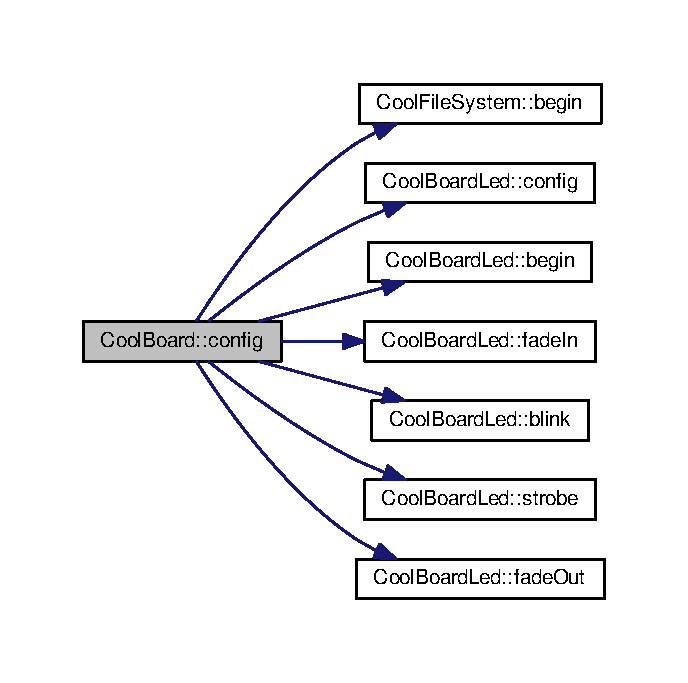
\includegraphics[width=350pt]{d7/df9/class_cool_board_a583a874c09c07e70a6eb9229fc4beddb_cgraph}
\end{center}
\end{figure}
\mbox{\Hypertarget{class_cool_board_a519de78b807f8ec6463ff484eb925918}\label{class_cool_board_a519de78b807f8ec6463ff484eb925918}} 
\index{Cool\+Board@{Cool\+Board}!connect@{connect}}
\index{connect@{connect}!Cool\+Board@{Cool\+Board}}
\subsubsection{\texorpdfstring{connect()}{connect()}}
{\footnotesize\ttfamily int Cool\+Board\+::connect (\begin{DoxyParamCaption}{ }\end{DoxyParamCaption})}

\hyperlink{class_cool_board_a519de78b807f8ec6463ff484eb925918}{Cool\+Board\+::connect()}\+: This method is provided to manage the network connection and the mqtt connection.

\begin{DoxyReturn}{Returns}
mqtt client state 
\end{DoxyReturn}


Definition at line 224 of file Cool\+Board.\+cpp.


\begin{DoxyCode}
225 \{
226 
227 \textcolor{preprocessor}{#if DEBUG == 1  }
228 
229     Serial.println( F(\textcolor{stringliteral}{"Entering CoolBoard.connect "}) );
230     Serial.println();
231     Serial.println( F(\textcolor{stringliteral}{"Connecting the CoolBoard  "}) );
232     delay(100);
233 
234 \textcolor{preprocessor}{#endif}
235     \hyperlink{class_cool_board_a1b1d3c684a5baa56b08486e192fd8e97}{coolBoardLed}.\hyperlink{class_cool_board_led_a30fadd4cbec17ceea428bf7a32207e87}{write}(0,0,255);\textcolor{comment}{//blue}
236 
237     
238             
239     
240 \textcolor{preprocessor}{#if DEBUG == 1      }
241 
242     Serial.println( F(\textcolor{stringliteral}{"Launching CoolWifi"}) );
243     Serial.println();
244 
245 \textcolor{preprocessor}{#endif}
246     \hyperlink{class_cool_board_acd88e6003606b47479ebba81e4aceeca}{wifiManager}.\hyperlink{class_cool_wifi_ad060353050f40d032a2dbf9e54a768bf}{connect}();
247     delay(100);
248 
249 
250     \textcolor{comment}{//only attempt MQTT connection when Wifi is Connected}
251     \textcolor{keywordflow}{if} (\hyperlink{class_cool_board_acd88e6003606b47479ebba81e4aceeca}{wifiManager}.\hyperlink{class_cool_wifi_a1c7b4d82a4098d346e7593dce92039fa}{state}() == WL\_CONNECTED)
252     \{
253 
254 \textcolor{preprocessor}{    #if DEBUG == 1  }
255     
256         Serial.println( F(\textcolor{stringliteral}{"Launching mqtt.connect()"}) );
257         Serial.println();
258     
259 \textcolor{preprocessor}{    #endif  }
260         \textcolor{comment}{//logInterval in seconds}
261         \hyperlink{class_cool_board_a2399f44d7c23c1149a335cb3b46d90f1}{mqtt}.\hyperlink{class_cool_m_q_t_t_a50075d0ab23a327ab897fd6adad20eda}{connect}(\textcolor{keyword}{this} -> \hyperlink{class_cool_board_a7508e029f2ee17bb747ffab599285e0d}{getLogInterval}()*2);
262         delay(100);
263     \}
264     
265         
266     
267     
268 \textcolor{preprocessor}{#if DEBUG == 1}
269 
270     Serial.println( F(\textcolor{stringliteral}{"mqtt state is :"}) );
271     Serial.println(\hyperlink{class_cool_board_a2399f44d7c23c1149a335cb3b46d90f1}{mqtt}.\hyperlink{class_cool_m_q_t_t_a5d003307eff78efbd585e42b43b72b6d}{state}());
272     Serial.println();
273     delay(100);
274 
275 \textcolor{preprocessor}{#endif}
276 
277     \hyperlink{class_cool_board_a1b1d3c684a5baa56b08486e192fd8e97}{coolBoardLed}.\hyperlink{class_cool_board_led_a96e1ea13003eee34c9dbcef340404426}{blink}(0,0,255,0.5);\textcolor{comment}{//blue}
278 
279     \textcolor{keywordflow}{return}(\hyperlink{class_cool_board_a2399f44d7c23c1149a335cb3b46d90f1}{mqtt}.\hyperlink{class_cool_m_q_t_t_a5d003307eff78efbd585e42b43b72b6d}{state}());
280 \}
\end{DoxyCode}
Here is the call graph for this function\+:
\nopagebreak
\begin{figure}[H]
\begin{center}
\leavevmode
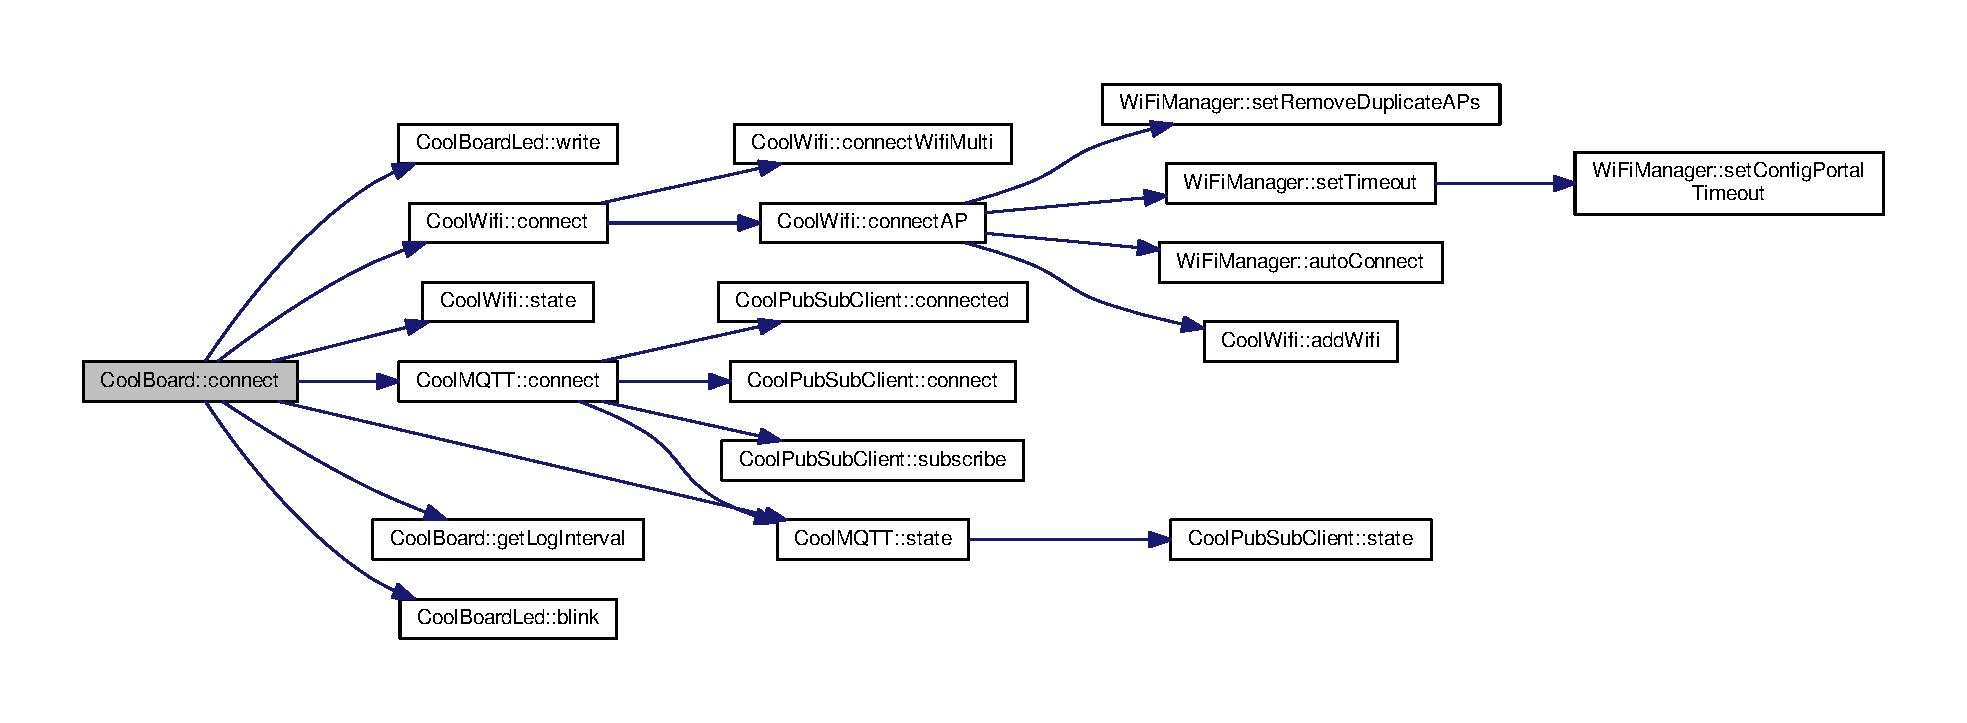
\includegraphics[width=350pt]{d7/df9/class_cool_board_a519de78b807f8ec6463ff484eb925918_cgraph}
\end{center}
\end{figure}
Here is the caller graph for this function\+:
\nopagebreak
\begin{figure}[H]
\begin{center}
\leavevmode
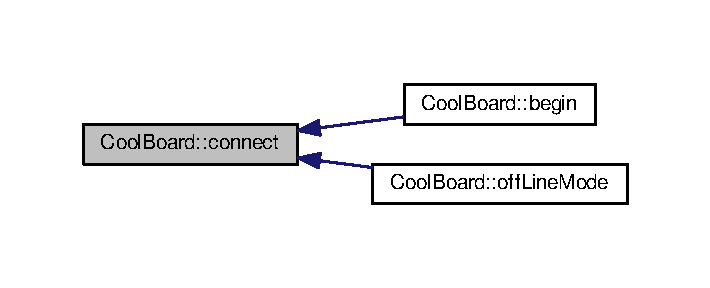
\includegraphics[width=341pt]{d7/df9/class_cool_board_a519de78b807f8ec6463ff484eb925918_icgraph}
\end{center}
\end{figure}
\mbox{\Hypertarget{class_cool_board_a7508e029f2ee17bb747ffab599285e0d}\label{class_cool_board_a7508e029f2ee17bb747ffab599285e0d}} 
\index{Cool\+Board@{Cool\+Board}!get\+Log\+Interval@{get\+Log\+Interval}}
\index{get\+Log\+Interval@{get\+Log\+Interval}!Cool\+Board@{Cool\+Board}}
\subsubsection{\texorpdfstring{get\+Log\+Interval()}{getLogInterval()}}
{\footnotesize\ttfamily unsigned long Cool\+Board\+::get\+Log\+Interval (\begin{DoxyParamCaption}{ }\end{DoxyParamCaption})}

\hyperlink{class_cool_board_a7508e029f2ee17bb747ffab599285e0d}{Cool\+Board\+::get\+Log\+Interval()}\+: This method is provided to get the log interval

\begin{DoxyReturn}{Returns}
interval value in s 
\end{DoxyReturn}


Definition at line 1129 of file Cool\+Board.\+cpp.


\begin{DoxyCode}
1130 \{
1131 
1132 \textcolor{preprocessor}{#if DEBUG == 1}
1133 
1134     Serial.println( F(\textcolor{stringliteral}{"Entering CoolBoard.getLogInterval() "}) );
1135     Serial.println();
1136     Serial.println( F(\textcolor{stringliteral}{"log Interval is :"}) );
1137     Serial.println(\hyperlink{class_cool_board_a84bc94413b64973e4aba8c467c97006c}{logInterval});
1138     Serial.println();
1139 
1140 \textcolor{preprocessor}{#endif}
1141 
1142     \textcolor{keywordflow}{return}(\textcolor{keyword}{this} -> \hyperlink{class_cool_board_a84bc94413b64973e4aba8c467c97006c}{logInterval});
1143 \}
\end{DoxyCode}
Here is the caller graph for this function\+:
\nopagebreak
\begin{figure}[H]
\begin{center}
\leavevmode
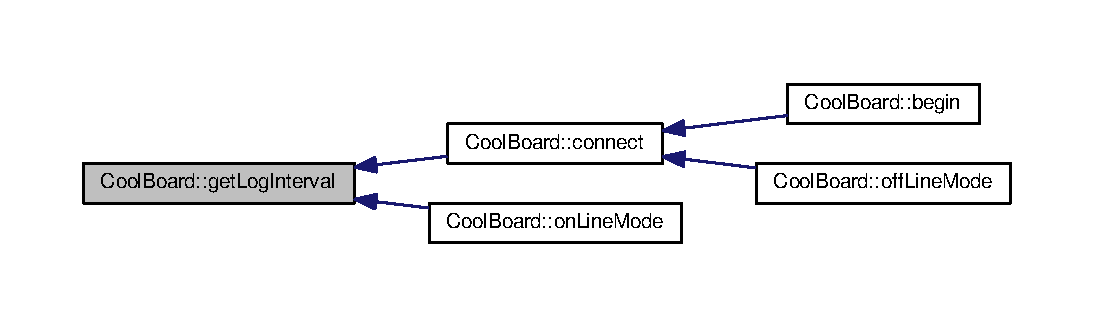
\includegraphics[width=350pt]{d7/df9/class_cool_board_a7508e029f2ee17bb747ffab599285e0d_icgraph}
\end{center}
\end{figure}
\mbox{\Hypertarget{class_cool_board_a397b46fadab8f530a8cf4d914c561366}\label{class_cool_board_a397b46fadab8f530a8cf4d914c561366}} 
\index{Cool\+Board@{Cool\+Board}!init\+Read\+I2C@{init\+Read\+I2C}}
\index{init\+Read\+I2C@{init\+Read\+I2C}!Cool\+Board@{Cool\+Board}}
\subsubsection{\texorpdfstring{init\+Read\+I2\+C()}{initReadI2C()}}
{\footnotesize\ttfamily void Cool\+Board\+::init\+Read\+I2C (\begin{DoxyParamCaption}{ }\end{DoxyParamCaption})}

\hyperlink{class_cool_board_a397b46fadab8f530a8cf4d914c561366}{Cool\+Board\+::init\+Read\+I2\+C()}\+: This method is provided to enable the I2C Interface. 

Definition at line 1224 of file Cool\+Board.\+cpp.


\begin{DoxyCode}
1225 \{
1226 
1227 \textcolor{preprocessor}{#if DEBUG == 1}
1228 
1229     Serial.println( F(\textcolor{stringliteral}{"Entering CoolBoard.initReadI2C()"}) );
1230     Serial.println();
1231 
1232 \textcolor{preprocessor}{#endif}
1233  
1234     digitalWrite(\hyperlink{class_cool_board_af1fe1376fc66f93dee80b327ca695377}{EnI2C},HIGH);\textcolor{comment}{//HIGH= I2C Enable}
1235 
1236 \}
\end{DoxyCode}
Here is the caller graph for this function\+:
\nopagebreak
\begin{figure}[H]
\begin{center}
\leavevmode
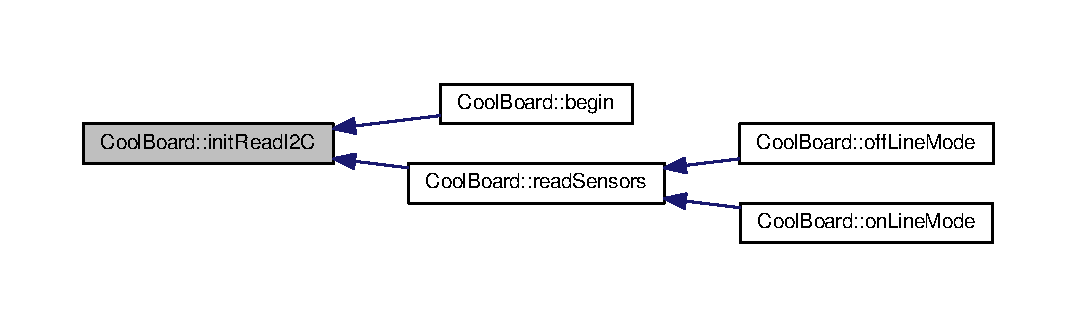
\includegraphics[width=350pt]{d7/df9/class_cool_board_a397b46fadab8f530a8cf4d914c561366_icgraph}
\end{center}
\end{figure}
\mbox{\Hypertarget{class_cool_board_ad7442cf4b62c7b0d5bd62a0f75ffc065}\label{class_cool_board_ad7442cf4b62c7b0d5bd62a0f75ffc065}} 
\index{Cool\+Board@{Cool\+Board}!is\+Connected@{is\+Connected}}
\index{is\+Connected@{is\+Connected}!Cool\+Board@{Cool\+Board}}
\subsubsection{\texorpdfstring{is\+Connected()}{isConnected()}}
{\footnotesize\ttfamily int Cool\+Board\+::is\+Connected (\begin{DoxyParamCaption}{ }\end{DoxyParamCaption})}

\hyperlink{class_cool_board_ad7442cf4b62c7b0d5bd62a0f75ffc065}{Cool\+Board\+::is\+Connected()}

This method is provided to check if the card is connected to Wifi and M\+Q\+TT

\begin{DoxyReturn}{Returns}
0 \+: connected -\/1\+: Wifi Not Connected -\/2\+: M\+Q\+TT Not Connected 
\end{DoxyReturn}


Definition at line 176 of file Cool\+Board.\+cpp.


\begin{DoxyCode}
177 \{
178 
179 \textcolor{preprocessor}{#if DEBUG == 1  }
180 
181     Serial.println( F(\textcolor{stringliteral}{"Entering CoolBoard.isConnected "}) );
182     Serial.println();
183 
184 \textcolor{preprocessor}{#endif}
185     \textcolor{keywordflow}{if} (\hyperlink{class_cool_board_acd88e6003606b47479ebba81e4aceeca}{wifiManager}.\hyperlink{class_cool_wifi_a1c7b4d82a4098d346e7593dce92039fa}{state}() != WL\_CONNECTED)
186     \{
187     
188         Serial.println(F(\textcolor{stringliteral}{"Wifi Not Connected"}));
189 
190 \textcolor{preprocessor}{    #if DEBUG == 1}
191 
192         Serial.println(F(\textcolor{stringliteral}{"Wifi State is "}));
193         Serial.println(\hyperlink{class_cool_board_acd88e6003606b47479ebba81e4aceeca}{wifiManager}.\hyperlink{class_cool_wifi_a1c7b4d82a4098d346e7593dce92039fa}{state}());
194         
195 \textcolor{preprocessor}{    #endif}
196         \textcolor{keywordflow}{return}(-1);
197     \}
198     
199     \textcolor{keywordflow}{if}(\hyperlink{class_cool_board_a2399f44d7c23c1149a335cb3b46d90f1}{mqtt}.\hyperlink{class_cool_m_q_t_t_a5d003307eff78efbd585e42b43b72b6d}{state}() != 0)
200     \{
201         
202         Serial.println( F(\textcolor{stringliteral}{"MQTT not Connected"}));
203 
204 \textcolor{preprocessor}{    #if DEBUG==1}
205         Serial.println( F(\textcolor{stringliteral}{"mqtt state is :"}) );
206         Serial.println(\hyperlink{class_cool_board_a2399f44d7c23c1149a335cb3b46d90f1}{mqtt}.\hyperlink{class_cool_m_q_t_t_a5d003307eff78efbd585e42b43b72b6d}{state}());  
207     
208 \textcolor{preprocessor}{    #endif}
209 
210     \}
211     
212     \textcolor{keywordflow}{return}(0);
213 
214 \}
\end{DoxyCode}
Here is the call graph for this function\+:
\nopagebreak
\begin{figure}[H]
\begin{center}
\leavevmode
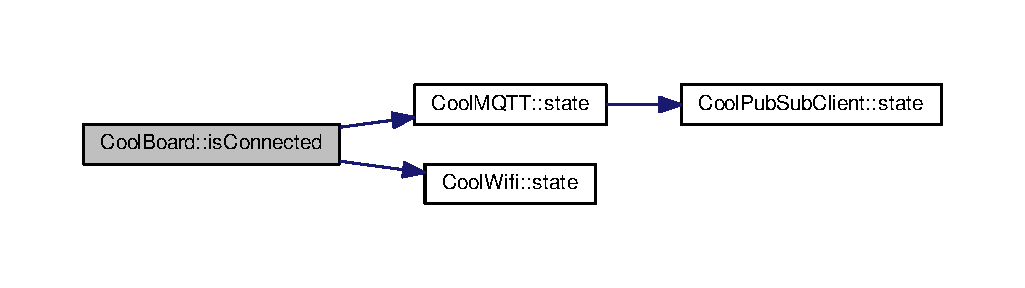
\includegraphics[width=350pt]{d7/df9/class_cool_board_ad7442cf4b62c7b0d5bd62a0f75ffc065_cgraph}
\end{center}
\end{figure}
\mbox{\Hypertarget{class_cool_board_ae6b5e1274d760462290192acea4adca8}\label{class_cool_board_ae6b5e1274d760462290192acea4adca8}} 
\index{Cool\+Board@{Cool\+Board}!off\+Line\+Mode@{off\+Line\+Mode}}
\index{off\+Line\+Mode@{off\+Line\+Mode}!Cool\+Board@{Cool\+Board}}
\subsubsection{\texorpdfstring{off\+Line\+Mode()}{offLineMode()}}
{\footnotesize\ttfamily void Cool\+Board\+::off\+Line\+Mode (\begin{DoxyParamCaption}{ }\end{DoxyParamCaption})}

Cool\+Board\+::offline\+Mode()\+: This method is provided to manage the off\+Line mode\+: -\/read sensors -\/do actions -\/save data in the file system -\/if there is Wi\+Fi but no Internet \+: make data available over AP -\/if there is no connection \+: retry to connect 

Definition at line 551 of file Cool\+Board.\+cpp.


\begin{DoxyCode}
552 \{
553     \hyperlink{class_cool_board_a1b1d3c684a5baa56b08486e192fd8e97}{coolBoardLed}.\hyperlink{class_cool_board_led_af1cacbaa88db8bcf6042c1083ba41155}{fade}(51,100,50,0.5);\textcolor{comment}{//dark shade of green  }
554 \textcolor{preprocessor}{#if DEBUG == 1  }
555     
556     Serial.println( F(\textcolor{stringliteral}{"Entering off line mode "}) ); 
557     
558 \textcolor{preprocessor}{#endif}
559 
560 \textcolor{preprocessor}{#if DEBUG == 0}
561 
562     Serial.println( F(\textcolor{stringliteral}{"CoolBoard is in Offline Mode"}));
563 
564 \textcolor{preprocessor}{#endif}
565 
566     \textcolor{comment}{//read user data if user is active}
567     \textcolor{keywordflow}{if}(\hyperlink{class_cool_board_a6395459131d6889a3005f79c7a35e964}{userActive})
568     \{
569 
570         \hyperlink{class_cool_board_a1b1d3c684a5baa56b08486e192fd8e97}{coolBoardLed}.\hyperlink{class_cool_board_led_ab778f5e7bed0ab74e3906d82110493c3}{fadeIn}(245,237,27,0.5);\textcolor{comment}{//shade of yellow}
571 
572 \textcolor{preprocessor}{    #if DEBUG == 1}
573         
574         Serial.println( F(\textcolor{stringliteral}{"User is Active"}) );
575         Serial.println( F(\textcolor{stringliteral}{"Collecting User's data ( mac,username,timeStamp )"}) );
576         Serial.println();
577 
578 \textcolor{preprocessor}{    #endif}
579 
580         \hyperlink{class_cool_board_a1b1d3c684a5baa56b08486e192fd8e97}{coolBoardLed}.\hyperlink{class_cool_board_led_a96e1ea13003eee34c9dbcef340404426}{blink}(245,237,27,0.5);\textcolor{comment}{//shade of yellow   }
581 
582         \textcolor{comment}{//reading user data}
583         \hyperlink{class_cool_board_a427fb753dd8575bdf821c70a5c63d695}{data}=this->\hyperlink{class_cool_board_ae7358fb6e623cfc81b775f5f1734909b}{userData}();\textcolor{comment}{//\{"":"","":"","",""\}}
584 
585         \textcolor{comment}{//formatting json }
586         \hyperlink{class_cool_board_a427fb753dd8575bdf821c70a5c63d695}{data}.setCharAt( \hyperlink{class_cool_board_a427fb753dd8575bdf821c70a5c63d695}{data}.lastIndexOf(\textcolor{charliteral}{'\}'}) , \textcolor{charliteral}{','});\textcolor{comment}{//\{"":"","":"","","",}
587         
588                 
589         \textcolor{comment}{//read sensors data}
590 
591         Serial.println( F(\textcolor{stringliteral}{"Collecting sensors data "}) );
592         Serial.println();
593 
594         \hyperlink{class_cool_board_a427fb753dd8575bdf821c70a5c63d695}{data}+=this->\hyperlink{class_cool_board_ad03abdce2e65f520bbf2cff0f2d083cf}{readSensors}();\textcolor{comment}{//\{"":"","":"","","",\{.......\}}
595 
596         
597 
598         \textcolor{comment}{//formatting json correctly}
599         \hyperlink{class_cool_board_a427fb753dd8575bdf821c70a5c63d695}{data}.remove(\hyperlink{class_cool_board_a427fb753dd8575bdf821c70a5c63d695}{data}.lastIndexOf(\textcolor{charliteral}{'\{'}), 1);\textcolor{comment}{//\{"":"","":"","","",.......\}}
600 
601         \hyperlink{class_cool_board_a1b1d3c684a5baa56b08486e192fd8e97}{coolBoardLed}.\hyperlink{class_cool_board_led_a93d545679237e8cc858324367149775c}{fadeOut}(245,237,27,0.5);\textcolor{comment}{//shade of yellow}
602                 
603     \}   
604     \textcolor{keywordflow}{else}
605     \{
606         \textcolor{comment}{//read sensors data}
607 \textcolor{preprocessor}{    #if DEBUG == 1}
608 
609         Serial.println( F(\textcolor{stringliteral}{"Collecting sensors data "}) );
610         Serial.println();
611 
612 \textcolor{preprocessor}{    #endif}
613 
614         \hyperlink{class_cool_board_a1b1d3c684a5baa56b08486e192fd8e97}{coolBoardLed}.\hyperlink{class_cool_board_led_af1cacbaa88db8bcf6042c1083ba41155}{fade}(190,100,150,0.5);\textcolor{comment}{//shade of violet        }
615 
616         \hyperlink{class_cool_board_a427fb753dd8575bdf821c70a5c63d695}{data}=this->\hyperlink{class_cool_board_ad03abdce2e65f520bbf2cff0f2d083cf}{readSensors}();\textcolor{comment}{//\{..,..,..\}}
617     \}
618 
619     \hyperlink{class_cool_board_a1b1d3c684a5baa56b08486e192fd8e97}{coolBoardLed}.\hyperlink{class_cool_board_led_af1cacbaa88db8bcf6042c1083ba41155}{fade}(51,100,50,0.5);\textcolor{comment}{//dark shade of green  }
620 
621     \textcolor{comment}{//do action}
622 
623     \textcolor{keywordflow}{if} (\hyperlink{class_cool_board_a9be03a913d26e558328935ca3b59a75e}{jetpackActive})
624     \{
625     
626 
627 
628 \textcolor{preprocessor}{    #if DEBUG == 1}
629 
630         Serial.println( F(\textcolor{stringliteral}{"jetpack is Active "}) );
631         Serial.println( F(\textcolor{stringliteral}{"jetpack doing action "}) );
632         Serial.println();
633     
634 \textcolor{preprocessor}{    #endif}
635         \hyperlink{class_cool_board_a1b1d3c684a5baa56b08486e192fd8e97}{coolBoardLed}.\hyperlink{class_cool_board_led_af1cacbaa88db8bcf6042c1083ba41155}{fade}(100,100,150,0.5);\textcolor{comment}{//dark shade of blue }
636     
637         \hyperlink{class_cool_board_a30b1357881b01ccbec676856a91e48e9}{jetPack}.\hyperlink{class_jetpack_a9e703197093094b963f9ad57817495b8}{doAction}( \hyperlink{class_cool_board_a427fb753dd8575bdf821c70a5c63d695}{data}.c\_str() );
638     \}
639     
640     delay(100);
641 
642     \hyperlink{class_cool_board_a4ac693895c21025b8808653f2a4316e6}{onBoardActor}.\hyperlink{class_cool_board_actor_a96a45658d32c6b95caa2f385c7da32cd}{doAction}( \hyperlink{class_cool_board_a427fb753dd8575bdf821c70a5c63d695}{data}.c\_str() );  
643 
644 
645     \hyperlink{class_cool_board_a1b1d3c684a5baa56b08486e192fd8e97}{coolBoardLed}.\hyperlink{class_cool_board_led_af1cacbaa88db8bcf6042c1083ba41155}{fade}(51,100,50,0.5);\textcolor{comment}{//dark shade of green  }
646     
647     \textcolor{comment}{//saving data in the file system}
648     
649     \hyperlink{class_cool_board_a42c2586fbb13ff7f06538e9284e8538d}{fileSystem}.\hyperlink{class_cool_file_system_afa3a4feae94871d4d3b6bebb701c2e67}{saveSensorData}( \hyperlink{class_cool_board_a427fb753dd8575bdf821c70a5c63d695}{data}.c\_str() );
650 
651 \textcolor{preprocessor}{    #if DEBUG == 0}
652 
653         Serial.println( F(\textcolor{stringliteral}{"saving Data in Memory : OK"}));
654 
655 \textcolor{preprocessor}{    #endif}
656 
657     \hyperlink{class_cool_board_a1b1d3c684a5baa56b08486e192fd8e97}{coolBoardLed}.\hyperlink{class_cool_board_led_a93d545679237e8cc858324367149775c}{fadeOut}(51,100,50,0.5);\textcolor{comment}{//dark shade of green}
658 
659     \textcolor{comment}{//case we have wifi but no internet}
660     \textcolor{keywordflow}{if}( (\hyperlink{class_cool_board_acd88e6003606b47479ebba81e4aceeca}{wifiManager}.\hyperlink{class_cool_wifi_a1c7b4d82a4098d346e7593dce92039fa}{state}() == WL\_CONNECTED) && ( \hyperlink{class_cool_board_a2399f44d7c23c1149a335cb3b46d90f1}{mqtt}.
      \hyperlink{class_cool_m_q_t_t_a5d003307eff78efbd585e42b43b72b6d}{state}()!=0 ) )
661     \{
662         
663         Serial.println(F(\textcolor{stringliteral}{"there is Wifi but no Internet"}));
664         Serial.println(F(\textcolor{stringliteral}{"lunching AP to check saved files"}));
665         Serial.println(F(\textcolor{stringliteral}{"and Add new WiFi if needed"}));
666         
667         \hyperlink{class_cool_board_acd88e6003606b47479ebba81e4aceeca}{wifiManager}.\hyperlink{class_cool_wifi_a7c857f27161782f5ef1d62d552aff971}{connectAP}();
668         
669     \}
670     
671     \textcolor{comment}{//case we have no connection at all}
672     \textcolor{keywordflow}{if}( \hyperlink{class_cool_board_acd88e6003606b47479ebba81e4aceeca}{wifiManager}.\hyperlink{class_cool_wifi_a1c7b4d82a4098d346e7593dce92039fa}{state}() != WL\_CONNECTED )
673     \{
674     
675 \textcolor{preprocessor}{    #if DEBUG == 1}
676         
677         Serial.println(F(\textcolor{stringliteral}{"there is No Wifi "}));
678         Serial.println(F(\textcolor{stringliteral}{"retrying to connect"}));
679     
680 \textcolor{preprocessor}{    #endif}
681 
682 \textcolor{preprocessor}{    #if DEBUG == 0}
683         Serial.println( F(\textcolor{stringliteral}{"there is no WiFi..."}));
684 \textcolor{preprocessor}{    #endif}
685         
686         this->\hyperlink{class_cool_board_a519de78b807f8ec6463ff484eb925918}{connect}();\textcolor{comment}{//nomad case : just run wifiMulti}
687                 \textcolor{comment}{//normal case : run wifiMulti+AP}
688         
689     \}   
690 
691 \}
\end{DoxyCode}
Here is the call graph for this function\+:
\nopagebreak
\begin{figure}[H]
\begin{center}
\leavevmode
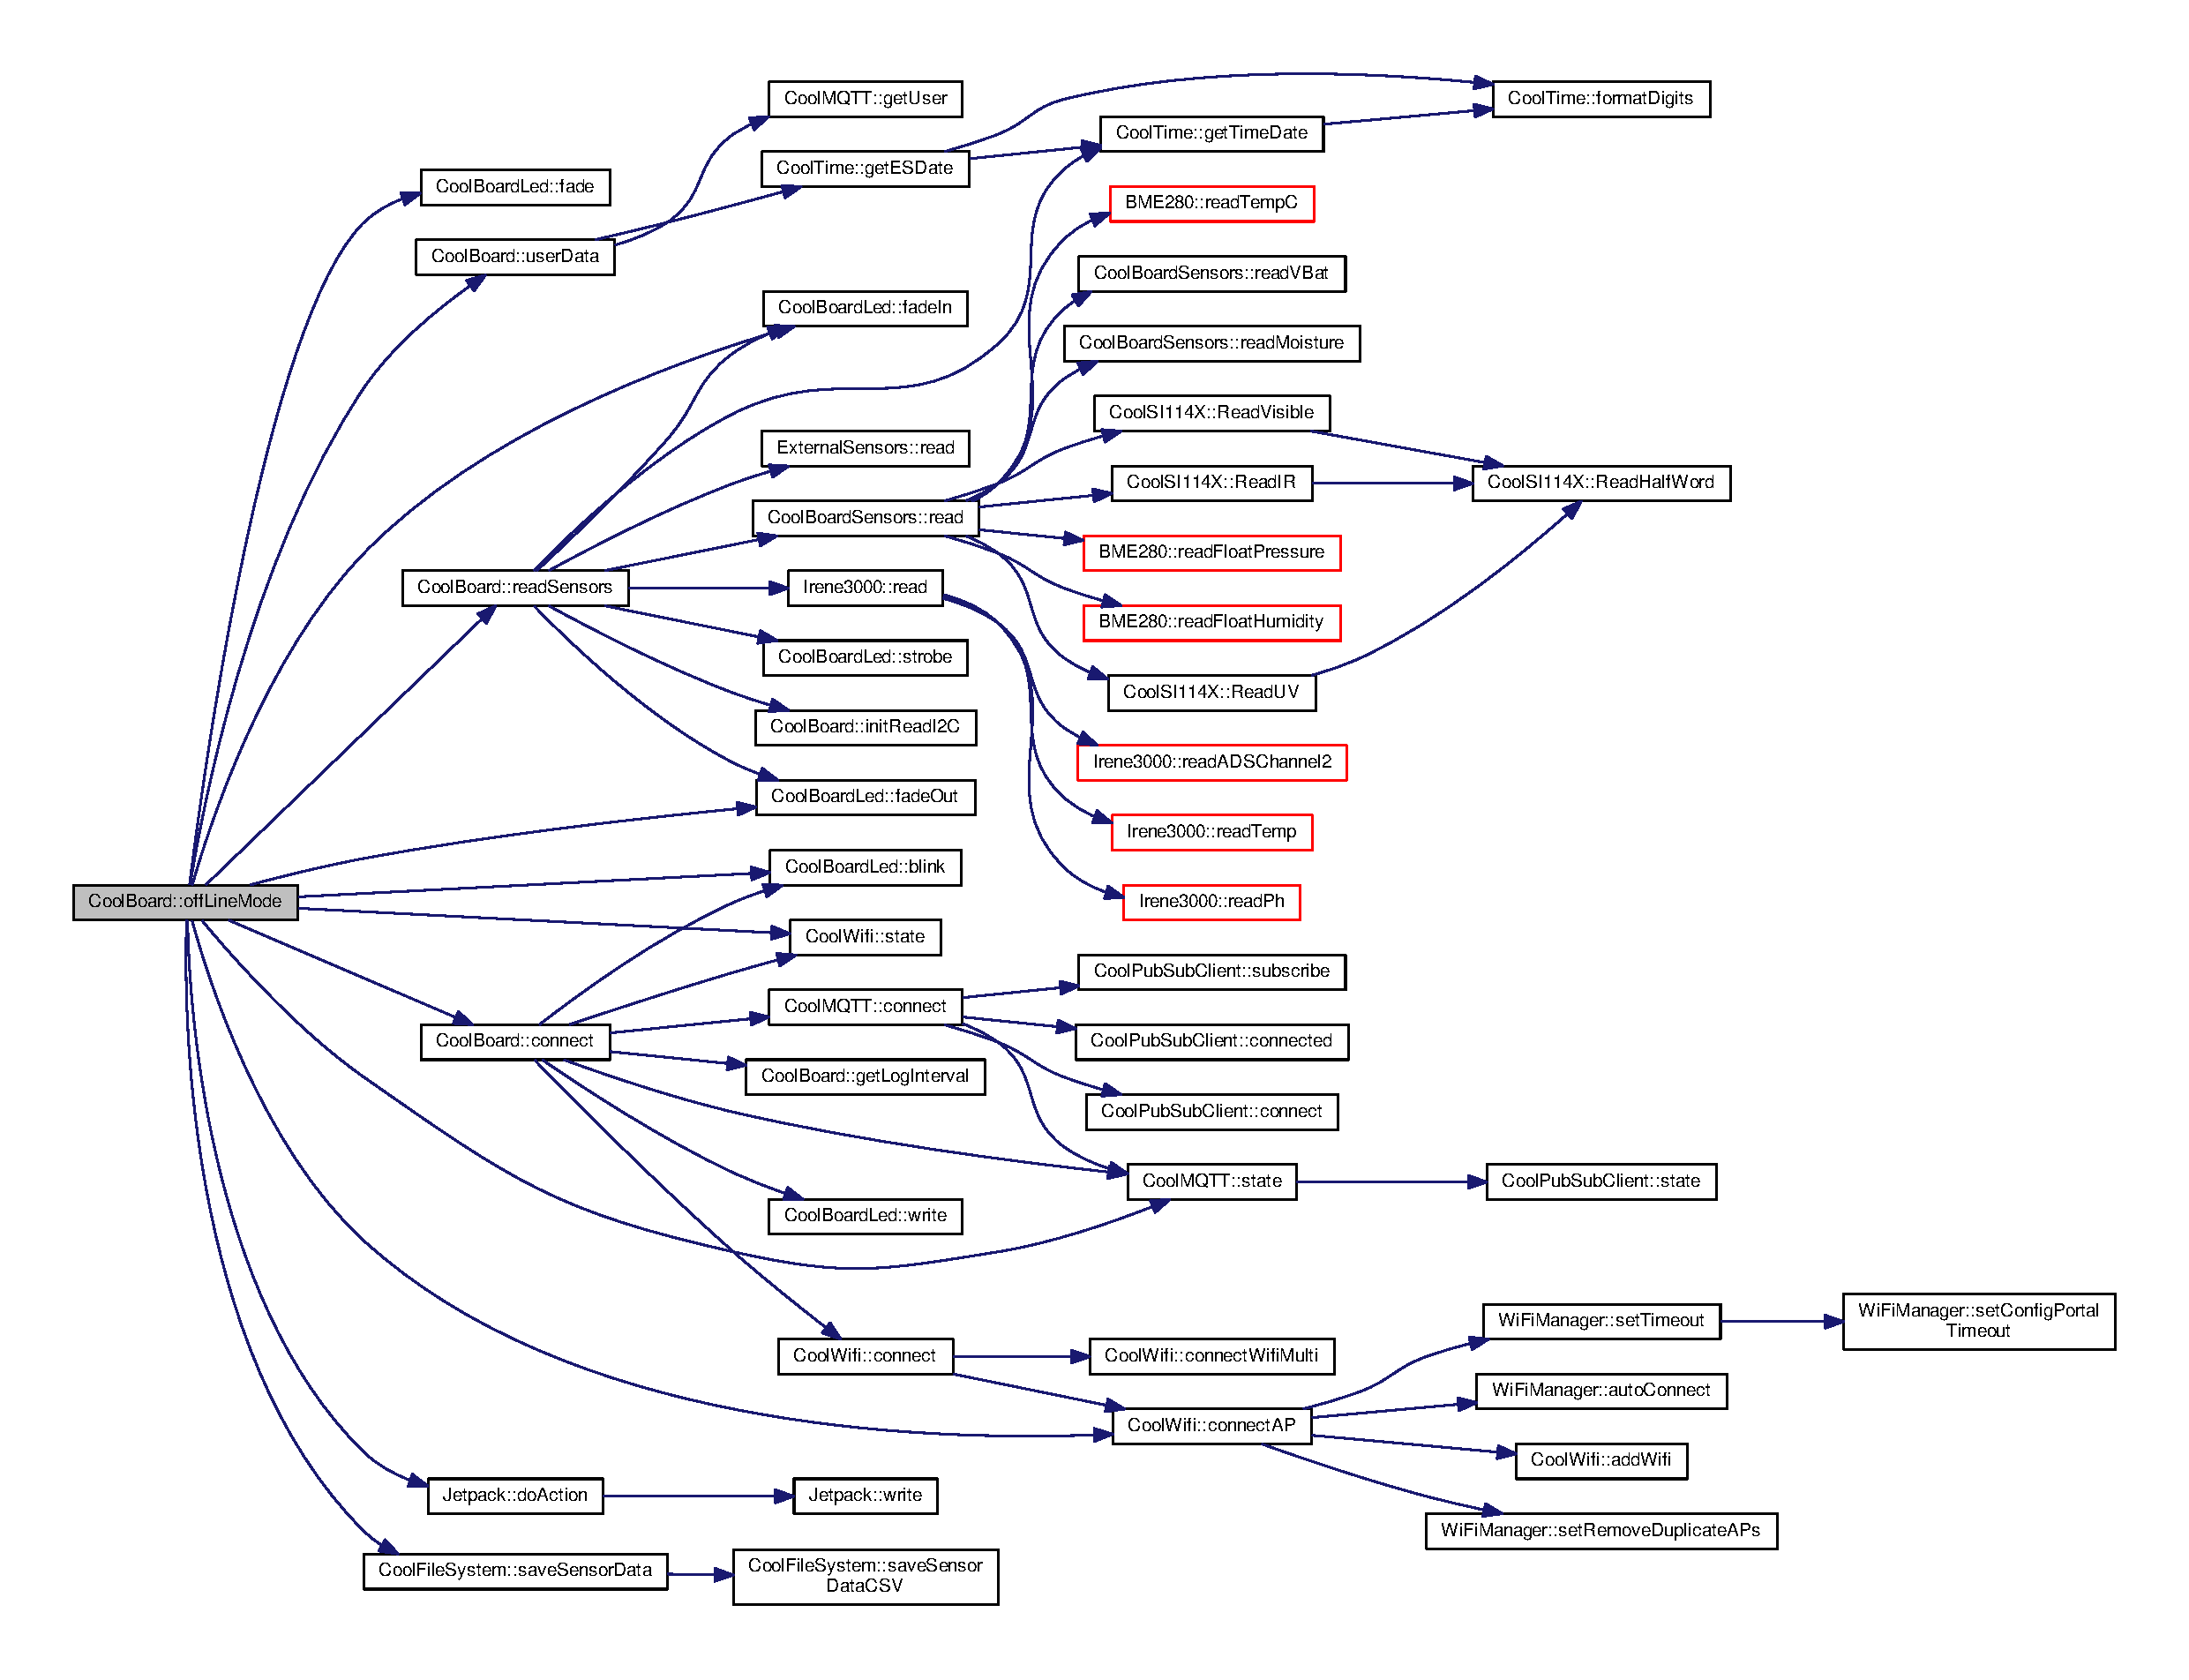
\includegraphics[width=350pt]{d7/df9/class_cool_board_ae6b5e1274d760462290192acea4adca8_cgraph}
\end{center}
\end{figure}
\mbox{\Hypertarget{class_cool_board_aa0bbc4bc605e35618d18e68795c61363}\label{class_cool_board_aa0bbc4bc605e35618d18e68795c61363}} 
\index{Cool\+Board@{Cool\+Board}!on\+Line\+Mode@{on\+Line\+Mode}}
\index{on\+Line\+Mode@{on\+Line\+Mode}!Cool\+Board@{Cool\+Board}}
\subsubsection{\texorpdfstring{on\+Line\+Mode()}{onLineMode()}}
{\footnotesize\ttfamily void Cool\+Board\+::on\+Line\+Mode (\begin{DoxyParamCaption}{ }\end{DoxyParamCaption})}

\hyperlink{class_cool_board_aa0bbc4bc605e35618d18e68795c61363}{Cool\+Board\+::on\+Line\+Mode()}\+: This method is provided to manage the online mode\+: -\/update clock -\/read sensor -\/do actions -\/publish data -\/read answer -\/update config 

Definition at line 292 of file Cool\+Board.\+cpp.


\begin{DoxyCode}
293 \{
294 
295     \hyperlink{class_cool_board_a1b1d3c684a5baa56b08486e192fd8e97}{coolBoardLed}.\hyperlink{class_cool_board_led_ab778f5e7bed0ab74e3906d82110493c3}{fadeIn}(128,255,50,0.5);\textcolor{comment}{//shade of green}
296 
297 \textcolor{preprocessor}{#if DEBUG == 1}
298 
299     Serial.println( F(\textcolor{stringliteral}{"Entering CoolBoard.onLineMode() "}) );
300     Serial.println();
301 
302 \textcolor{preprocessor}{#endif}
303 \textcolor{preprocessor}{#if DEBUG == 0}
304 
305     Serial.println( F(\textcolor{stringliteral}{"CoolBoard is in Online Mode"}));
306 
307 \textcolor{preprocessor}{#endif}
308 
309     \hyperlink{class_cool_board_a427fb753dd8575bdf821c70a5c63d695}{data}=\textcolor{stringliteral}{""};
310     \hyperlink{class_cool_board_a7b835fafd449e5282f7f91d787a2dc15}{answer}=\textcolor{stringliteral}{""};
311 
312     \textcolor{comment}{//send saved data if any}
313     \textcolor{keywordflow}{if}(\hyperlink{class_cool_board_a42c2586fbb13ff7f06538e9284e8538d}{fileSystem}.\hyperlink{class_cool_file_system_ac86a40e7c3a1842f7342f698d34324f9}{isDataSaved}())
314     \{
315 
316         \hyperlink{class_cool_board_a1b1d3c684a5baa56b08486e192fd8e97}{coolBoardLed}.\hyperlink{class_cool_board_led_ab778f5e7bed0ab74e3906d82110493c3}{fadeIn}(128,128,255,0.5);\textcolor{comment}{//shade of blue}
317 
318         Serial.println( F(\textcolor{stringliteral}{"There is data saved on the File System"}) );
319         Serial.println( F(\textcolor{stringliteral}{"Sending saved data over MQTT "}) );
320         Serial.println();
321         \hyperlink{class_cool_board_a1b1d3c684a5baa56b08486e192fd8e97}{coolBoardLed}.\hyperlink{class_cool_board_led_ad5f0de4c628cbfbf49896042831c64ad}{strobe}(128,128,255,0.5);\textcolor{comment}{//shade of blue }
322 
323         \hyperlink{class_cool_board_a2399f44d7c23c1149a335cb3b46d90f1}{mqtt}.\hyperlink{class_cool_m_q_t_t_ace977b3e90ab14b1199fe5c4fb0a13ec}{publish}(\textcolor{stringliteral}{"sending saved data"});
324         \hyperlink{class_cool_board_a2399f44d7c23c1149a335cb3b46d90f1}{mqtt}.\hyperlink{class_cool_m_q_t_t_aa5eaae967b562b62cbcf2b8d81f6e5d5}{mqttLoop}();
325 
326 
327         
328         \textcolor{keywordtype}{int} size=0;
329         std::unique\_ptr<String[]> savedData(std::move(\hyperlink{class_cool_board_a42c2586fbb13ff7f06538e9284e8538d}{fileSystem}.
      \hyperlink{class_cool_file_system_a3223ffff4266a6300988fab956d6b4b2}{getSensorSavedData}(size)));\textcolor{comment}{//\{..,..,..\}}
330 
331         \textcolor{keywordtype}{int} i=0;
332         \textcolor{comment}{//loop through the array}
333         \textcolor{keywordflow}{while}(i<size)
334         \{
335             \textcolor{comment}{//formatting data:}
336         
337             String jsonData = \textcolor{stringliteral}{"\{\(\backslash\)"state\(\backslash\)":\{\(\backslash\)"reported\(\backslash\)":"};
338             jsonData += savedData[i]; \textcolor{comment}{// \{"state":\{"reported":\{..,..,..,..,..,..,..,..\}}
339             jsonData += \textcolor{stringliteral}{" \} \}"}; \textcolor{comment}{// \{"state":\{"reported":\{..,..,..,..,..,..,..,..\}  \} \}}
340 
341 \textcolor{preprocessor}{        #if DEBUG == 1 }
342             Serial.println(F(\textcolor{stringliteral}{"Size is : "}));
343             Serial.println(size);
344             Serial.print(F(\textcolor{stringliteral}{"sending line N°"}));
345             Serial.println(i);
346             Serial.println(jsonData);
347             Serial.println();
348 
349 \textcolor{preprocessor}{        #endif}
350 
351             \hyperlink{class_cool_board_a1b1d3c684a5baa56b08486e192fd8e97}{coolBoardLed}.\hyperlink{class_cool_board_led_ad5f0de4c628cbfbf49896042831c64ad}{strobe}(128,128,255,0.5);\textcolor{comment}{//shade of blue}
352         
353             \hyperlink{class_cool_board_a2399f44d7c23c1149a335cb3b46d90f1}{mqtt}.\hyperlink{class_cool_m_q_t_t_ace977b3e90ab14b1199fe5c4fb0a13ec}{publish}( jsonData.c\_str() );
354             \hyperlink{class_cool_board_a2399f44d7c23c1149a335cb3b46d90f1}{mqtt}.\hyperlink{class_cool_m_q_t_t_aa5eaae967b562b62cbcf2b8d81f6e5d5}{mqttLoop}();
355         
356             \hyperlink{class_cool_board_a1b1d3c684a5baa56b08486e192fd8e97}{coolBoardLed}.\hyperlink{class_cool_board_led_a93d545679237e8cc858324367149775c}{fadeOut}(128,128,255,0.5);\textcolor{comment}{//shade of blue}
357             
358             i++;
359             yield();
360         \}       
361 
362 
363 \textcolor{preprocessor}{    #if DEBUG == 1}
364 
365         Serial.println( F(\textcolor{stringliteral}{"Saved data sent "}) );
366         Serial.println();
367     
368 \textcolor{preprocessor}{    #endif}
369 
370     \}
371 
372     \hyperlink{class_cool_board_a1b1d3c684a5baa56b08486e192fd8e97}{coolBoardLed}.\hyperlink{class_cool_board_led_a96e1ea13003eee34c9dbcef340404426}{blink}(128,255,50,0.5);\textcolor{comment}{//shade of green}
373 
374     \textcolor{comment}{//clock update}
375     Serial.println( F(\textcolor{stringliteral}{"Re-checking RTC..."}));
376     \hyperlink{class_cool_board_a50d2a6716879d64a85f3c6b44ad63275}{rtc}.\hyperlink{class_cool_time_aae601f795452cfa48d9fb337aed483a8}{update}();
377 
378     \textcolor{comment}{//read user data if user is active}
379     \textcolor{keywordflow}{if}(\hyperlink{class_cool_board_a6395459131d6889a3005f79c7a35e964}{userActive})
380     \{
381         \hyperlink{class_cool_board_a1b1d3c684a5baa56b08486e192fd8e97}{coolBoardLed}.\hyperlink{class_cool_board_led_ab778f5e7bed0ab74e3906d82110493c3}{fadeIn}(245,237,27,0.5);\textcolor{comment}{//shade of yellow}
382     
383 \textcolor{preprocessor}{    #if DEBUG == 1}
384 
385         Serial.println( F(\textcolor{stringliteral}{"User is Active"}) );
386         Serial.println( F(\textcolor{stringliteral}{"Collecting User's data ( mac,username,timeStamp )"}) );
387         Serial.println();
388     
389 \textcolor{preprocessor}{    #endif  }
390         \hyperlink{class_cool_board_a1b1d3c684a5baa56b08486e192fd8e97}{coolBoardLed}.\hyperlink{class_cool_board_led_a96e1ea13003eee34c9dbcef340404426}{blink}(245,237,27,0.5);\textcolor{comment}{//shade of yellow   }
391 
392         \textcolor{comment}{//reading user data}
393         \hyperlink{class_cool_board_a427fb753dd8575bdf821c70a5c63d695}{data}=this->\hyperlink{class_cool_board_ae7358fb6e623cfc81b775f5f1734909b}{userData}();\textcolor{comment}{//\{"":"","":"","",""\}}
394 
395         \textcolor{comment}{//formatting json }
396         \hyperlink{class_cool_board_a427fb753dd8575bdf821c70a5c63d695}{data}.setCharAt( \hyperlink{class_cool_board_a427fb753dd8575bdf821c70a5c63d695}{data}.lastIndexOf(\textcolor{charliteral}{'\}'}) , \textcolor{charliteral}{','});\textcolor{comment}{//\{"":"","":"","","",}
397                 
398         \textcolor{comment}{//read sensors data}
399 \textcolor{preprocessor}{    #if DEBUG == 1}
400 
401         Serial.println( F(\textcolor{stringliteral}{"Collecting sensors data "}) );
402         Serial.println();
403     
404 \textcolor{preprocessor}{    #endif}
405 
406         \hyperlink{class_cool_board_a427fb753dd8575bdf821c70a5c63d695}{data}+=this->\hyperlink{class_cool_board_ad03abdce2e65f520bbf2cff0f2d083cf}{readSensors}();\textcolor{comment}{//\{"":"","":"","","",\{.......\}     }
407 
408         \textcolor{comment}{//formatting json correctly}
409         \hyperlink{class_cool_board_a427fb753dd8575bdf821c70a5c63d695}{data}.remove(\hyperlink{class_cool_board_a427fb753dd8575bdf821c70a5c63d695}{data}.lastIndexOf(\textcolor{charliteral}{'\{'}), 1);\textcolor{comment}{//\{"":"","":"","","",.......\}}
410         
411         \hyperlink{class_cool_board_a1b1d3c684a5baa56b08486e192fd8e97}{coolBoardLed}.\hyperlink{class_cool_board_led_a93d545679237e8cc858324367149775c}{fadeOut}(245,237,27,0.5);\textcolor{comment}{//shade of yellow}
412                 
413     \}   
414     \textcolor{keywordflow}{else}
415     \{
416         \textcolor{comment}{//read sensors data}
417 \textcolor{preprocessor}{    #if DEBUG == 1}
418 
419         Serial.println( F(\textcolor{stringliteral}{"Collecting sensors data "}) );
420         Serial.println();
421     
422 \textcolor{preprocessor}{    #endif}
423         \hyperlink{class_cool_board_a1b1d3c684a5baa56b08486e192fd8e97}{coolBoardLed}.\hyperlink{class_cool_board_led_af1cacbaa88db8bcf6042c1083ba41155}{fade}(190,100,150,0.5);\textcolor{comment}{//shade of violet        }
424         \hyperlink{class_cool_board_a427fb753dd8575bdf821c70a5c63d695}{data}=this->\hyperlink{class_cool_board_ad03abdce2e65f520bbf2cff0f2d083cf}{readSensors}();\textcolor{comment}{//\{..,..,..\}}
425     \}
426     
427 
428 
429 
430     \textcolor{comment}{//do action}
431 
432     \textcolor{keywordflow}{if} (\hyperlink{class_cool_board_a9be03a913d26e558328935ca3b59a75e}{jetpackActive})
433     \{
434 
435 
436 \textcolor{preprocessor}{    #if DEBUG ==1}
437 
438         Serial.println( F(\textcolor{stringliteral}{"jetpack is Active "}) );
439         Serial.println();
440 
441 \textcolor{preprocessor}{    #endif}
442     
443         \textcolor{keywordflow}{if}(this->\hyperlink{class_cool_board_a7c8e505a5804b109e112d5a03df6ea2b}{manual} == 0 )
444         \{
445 
446             Serial.println( F(\textcolor{stringliteral}{"jetpack doing action "}) );
447 
448             \hyperlink{class_cool_board_a1b1d3c684a5baa56b08486e192fd8e97}{coolBoardLed}.\hyperlink{class_cool_board_led_af1cacbaa88db8bcf6042c1083ba41155}{fade}(100,100,150,0.5);\textcolor{comment}{//dark shade of blue     }
449 
450             \hyperlink{class_cool_board_a30b1357881b01ccbec676856a91e48e9}{jetPack}.\hyperlink{class_jetpack_a9e703197093094b963f9ad57817495b8}{doAction}(\hyperlink{class_cool_board_a427fb753dd8575bdf821c70a5c63d695}{data}.c\_str());
451             
452 
453         
454         \}
455         
456         \textcolor{keywordflow}{else} \textcolor{keywordflow}{if}(this->\hyperlink{class_cool_board_a7c8e505a5804b109e112d5a03df6ea2b}{manual} == 1 )
457         \{
458         
459             Serial.println(F(\textcolor{stringliteral}{"we are in manual mode"}));
460             \hyperlink{class_cool_board_a2399f44d7c23c1149a335cb3b46d90f1}{mqtt}.\hyperlink{class_cool_m_q_t_t_aa5eaae967b562b62cbcf2b8d81f6e5d5}{mqttLoop}();
461             \hyperlink{class_cool_board_a7b835fafd449e5282f7f91d787a2dc15}{answer} = \hyperlink{class_cool_board_a2399f44d7c23c1149a335cb3b46d90f1}{mqtt}.\hyperlink{class_cool_m_q_t_t_ae3c18f6ae9723746d32765f1c8f176ca}{read}();
462             \textcolor{keyword}{this} -> \hyperlink{class_cool_board_a8612756d3f73198cdde857a66f0fe690}{update}(\hyperlink{class_cool_board_a7b835fafd449e5282f7f91d787a2dc15}{answer}.c\_str());
463         \}
464     \}
465 
466     delay(100);
467 
468     \hyperlink{class_cool_board_a4ac693895c21025b8808653f2a4316e6}{onBoardActor}.\hyperlink{class_cool_board_actor_a96a45658d32c6b95caa2f385c7da32cd}{doAction}( \hyperlink{class_cool_board_a427fb753dd8575bdf821c70a5c63d695}{data}.c\_str() );  
469 
470 
471 
472     
473     \hyperlink{class_cool_board_a1b1d3c684a5baa56b08486e192fd8e97}{coolBoardLed}.\hyperlink{class_cool_board_led_ab778f5e7bed0ab74e3906d82110493c3}{fadeIn}(128,255,50,0.5);\textcolor{comment}{//shade of green}
474 
475     \textcolor{comment}{//formatting data:}
476     String jsonData = \textcolor{stringliteral}{"\{\(\backslash\)"state\(\backslash\)":\{\(\backslash\)"reported\(\backslash\)":"};
477     jsonData += \hyperlink{class_cool_board_a427fb753dd8575bdf821c70a5c63d695}{data}; \textcolor{comment}{// \{"state":\{"reported":\{..,..,..,..,..,..,..,..\}}
478     jsonData += \textcolor{stringliteral}{" \} \}"}; \textcolor{comment}{// \{"state":\{"reported":\{..,..,..,..,..,..,..,..\}  \} \}}
479     
480     \textcolor{comment}{//mqtt client loop to allow data handling}
481     \hyperlink{class_cool_board_a2399f44d7c23c1149a335cb3b46d90f1}{mqtt}.\hyperlink{class_cool_m_q_t_t_aa5eaae967b562b62cbcf2b8d81f6e5d5}{mqttLoop}();
482 
483     \hyperlink{class_cool_board_a1b1d3c684a5baa56b08486e192fd8e97}{coolBoardLed}.\hyperlink{class_cool_board_led_a96e1ea13003eee34c9dbcef340404426}{blink}(128,255,50,0.5);\textcolor{comment}{//shade of green    }
484 
485     \textcolor{comment}{//read mqtt answer}
486     \hyperlink{class_cool_board_a7b835fafd449e5282f7f91d787a2dc15}{answer} = \hyperlink{class_cool_board_a2399f44d7c23c1149a335cb3b46d90f1}{mqtt}.\hyperlink{class_cool_m_q_t_t_ae3c18f6ae9723746d32765f1c8f176ca}{read}();
487 
488 \textcolor{preprocessor}{#if DEBUG == 1 }
489 
490     Serial.println( F(\textcolor{stringliteral}{"checking if there's an MQTT message "})  );
491     Serial.println( F(\textcolor{stringliteral}{"answer is : "}) );    
492     Serial.println(\hyperlink{class_cool_board_a7b835fafd449e5282f7f91d787a2dc15}{answer});   
493     Serial.println();
494 
495 \textcolor{preprocessor}{#endif  }
496 
497     \hyperlink{class_cool_board_a1b1d3c684a5baa56b08486e192fd8e97}{coolBoardLed}.\hyperlink{class_cool_board_led_a93d545679237e8cc858324367149775c}{fadeOut}(128,255,50,0.5);\textcolor{comment}{//shade of green    }
498 
499     \textcolor{comment}{//check if the configuration needs update }
500     \textcolor{comment}{//and update it if needed }
501     \textcolor{keyword}{this} -> \hyperlink{class_cool_board_a8612756d3f73198cdde857a66f0fe690}{update}(\hyperlink{class_cool_board_a7b835fafd449e5282f7f91d787a2dc15}{answer}.c\_str());
502     
503     \hyperlink{class_cool_board_a1b1d3c684a5baa56b08486e192fd8e97}{coolBoardLed}.\hyperlink{class_cool_board_led_ab778f5e7bed0ab74e3906d82110493c3}{fadeIn}(128,255,50,0.5);\textcolor{comment}{//shade of green  }
504 
505     \textcolor{comment}{//publishing data   }
506     \textcolor{keywordflow}{if}( this->\hyperlink{class_cool_board_a0a51b2287139f66c738101fb53139230}{sleepActive}==0 )   
507     \{   
508         \hyperlink{class_cool_board_a1b1d3c684a5baa56b08486e192fd8e97}{coolBoardLed}.\hyperlink{class_cool_board_led_ad5f0de4c628cbfbf49896042831c64ad}{strobe}(255,0,230,0.5);\textcolor{comment}{//shade of pink}
509         
510         \textcolor{comment}{//logInterval in seconds}
511         \hyperlink{class_cool_board_a2399f44d7c23c1149a335cb3b46d90f1}{mqtt}.\hyperlink{class_cool_m_q_t_t_ace977b3e90ab14b1199fe5c4fb0a13ec}{publish}( jsonData.c\_str(), this->\hyperlink{class_cool_board_a7508e029f2ee17bb747ffab599285e0d}{getLogInterval}() );
512         \hyperlink{class_cool_board_a2399f44d7c23c1149a335cb3b46d90f1}{mqtt}.\hyperlink{class_cool_m_q_t_t_aa5eaae967b562b62cbcf2b8d81f6e5d5}{mqttLoop}();
513     
514     \}
515     \textcolor{keywordflow}{else}
516     \{
517         \hyperlink{class_cool_board_a1b1d3c684a5baa56b08486e192fd8e97}{coolBoardLed}.\hyperlink{class_cool_board_led_ad5f0de4c628cbfbf49896042831c64ad}{strobe}(230,255,0,0.5);\textcolor{comment}{//shade of yellow  }
518 
519         \hyperlink{class_cool_board_a2399f44d7c23c1149a335cb3b46d90f1}{mqtt}.\hyperlink{class_cool_m_q_t_t_ace977b3e90ab14b1199fe5c4fb0a13ec}{publish}(jsonData.c\_str());      
520         \hyperlink{class_cool_board_a2399f44d7c23c1149a335cb3b46d90f1}{mqtt}.\hyperlink{class_cool_m_q_t_t_aa5eaae967b562b62cbcf2b8d81f6e5d5}{mqttLoop}();
521         \hyperlink{class_cool_board_a7b835fafd449e5282f7f91d787a2dc15}{answer} = \hyperlink{class_cool_board_a2399f44d7c23c1149a335cb3b46d90f1}{mqtt}.\hyperlink{class_cool_m_q_t_t_ae3c18f6ae9723746d32765f1c8f176ca}{read}();
522         \textcolor{keyword}{this} ->update(\hyperlink{class_cool_board_a7b835fafd449e5282f7f91d787a2dc15}{answer}.c\_str());
523 
524         \textcolor{comment}{//logInterval in seconds}
525         this->\hyperlink{class_cool_board_a069952cdcb2e7f68518aa429eceadb6e}{sleep}( this->\hyperlink{class_cool_board_a7508e029f2ee17bb747ffab599285e0d}{getLogInterval}() ) ;
526     \}
527 
528     \hyperlink{class_cool_board_a1b1d3c684a5baa56b08486e192fd8e97}{coolBoardLed}.\hyperlink{class_cool_board_led_a93d545679237e8cc858324367149775c}{fadeOut}(128,255,50,0.5);\textcolor{comment}{//shade of green        }
529 
530     \hyperlink{class_cool_board_a2399f44d7c23c1149a335cb3b46d90f1}{mqtt}.\hyperlink{class_cool_m_q_t_t_aa5eaae967b562b62cbcf2b8d81f6e5d5}{mqttLoop}();
531 
532     \textcolor{comment}{//read mqtt answer}
533     \hyperlink{class_cool_board_a7b835fafd449e5282f7f91d787a2dc15}{answer} = \hyperlink{class_cool_board_a2399f44d7c23c1149a335cb3b46d90f1}{mqtt}.\hyperlink{class_cool_m_q_t_t_ae3c18f6ae9723746d32765f1c8f176ca}{read}();
534     \textcolor{keyword}{this} -> \hyperlink{class_cool_board_a8612756d3f73198cdde857a66f0fe690}{update}(\hyperlink{class_cool_board_a7b835fafd449e5282f7f91d787a2dc15}{answer}.c\_str()); 
535 
536     \hyperlink{class_cool_board_a1b1d3c684a5baa56b08486e192fd8e97}{coolBoardLed}.\hyperlink{class_cool_board_led_a96e1ea13003eee34c9dbcef340404426}{blink}(128,255,50,0.5);\textcolor{comment}{//shade of green    }
537 
538 
539 \}
\end{DoxyCode}
Here is the call graph for this function\+:
\nopagebreak
\begin{figure}[H]
\begin{center}
\leavevmode
\includegraphics[width=350pt]{d7/df9/class_cool_board_aa0bbc4bc605e35618d18e68795c61363_cgraph}
\end{center}
\end{figure}
\mbox{\Hypertarget{class_cool_board_a486507b8f0981d3cc671ed31c2145755}\label{class_cool_board_a486507b8f0981d3cc671ed31c2145755}} 
\index{Cool\+Board@{Cool\+Board}!print\+Conf@{print\+Conf}}
\index{print\+Conf@{print\+Conf}!Cool\+Board@{Cool\+Board}}
\subsubsection{\texorpdfstring{print\+Conf()}{printConf()}}
{\footnotesize\ttfamily void Cool\+Board\+::print\+Conf (\begin{DoxyParamCaption}{ }\end{DoxyParamCaption})}

\hyperlink{class_cool_board_a486507b8f0981d3cc671ed31c2145755}{Cool\+Board\+::print\+Conf()}\+: This method is provided to print the configuration to the Serial Monitor. 

Definition at line 899 of file Cool\+Board.\+cpp.


\begin{DoxyCode}
900 \{
901 
902 \textcolor{preprocessor}{#if DEBUG == 1}
903     
904     Serial.println( F(\textcolor{stringliteral}{"Entering CoolBoard.printConf() "}) );
905     Serial.println();
906 
907 \textcolor{preprocessor}{#endif}
908 
909     Serial.println( F(\textcolor{stringliteral}{"Printing Cool Board Configuration "}));
910     Serial.print( F(\textcolor{stringliteral}{"log interval       : "}));
911     Serial.println(this->\hyperlink{class_cool_board_a84bc94413b64973e4aba8c467c97006c}{logInterval});
912 
913     Serial.print( F(\textcolor{stringliteral}{"irene active       : "}));
914     Serial.println(this->\hyperlink{class_cool_board_a9c3f7ac625481ee2ae802a25d97a4ae0}{ireneActive});
915 
916     Serial.print( F(\textcolor{stringliteral}{"jetpack active     : "}));
917     Serial.println(this->\hyperlink{class_cool_board_a9be03a913d26e558328935ca3b59a75e}{jetpackActive});
918 
919     Serial.print( F(\textcolor{stringliteral}{"external sensors active    : "}));
920     Serial.println(this->\hyperlink{class_cool_board_a638b00b76aeb819ecfd4c10b8cdd7bb7}{externalSensorsActive});
921 
922     Serial.print( F(\textcolor{stringliteral}{"sleep active       : "}));
923     Serial.println(this->\hyperlink{class_cool_board_a0a51b2287139f66c738101fb53139230}{sleepActive});
924 
925     Serial.print( F(\textcolor{stringliteral}{"user active        : "}));
926     Serial.println(this->\hyperlink{class_cool_board_a6395459131d6889a3005f79c7a35e964}{userActive});
927 
928     Serial.print( F(\textcolor{stringliteral}{"manual active      : "}));
929     Serial.println(this->\hyperlink{class_cool_board_a7c8e505a5804b109e112d5a03df6ea2b}{manual});
930 
931     Serial.println();
932 
933 
934 
935 
936 \}
\end{DoxyCode}
\mbox{\Hypertarget{class_cool_board_ad03abdce2e65f520bbf2cff0f2d083cf}\label{class_cool_board_ad03abdce2e65f520bbf2cff0f2d083cf}} 
\index{Cool\+Board@{Cool\+Board}!read\+Sensors@{read\+Sensors}}
\index{read\+Sensors@{read\+Sensors}!Cool\+Board@{Cool\+Board}}
\subsubsection{\texorpdfstring{read\+Sensors()}{readSensors()}}
{\footnotesize\ttfamily String Cool\+Board\+::read\+Sensors (\begin{DoxyParamCaption}{ }\end{DoxyParamCaption})}

\hyperlink{class_cool_board_ad03abdce2e65f520bbf2cff0f2d083cf}{Cool\+Board\+::read\+Sensors()}\+: This method is provided to read and format all the sensors data in a single json.

\begin{DoxyReturn}{Returns}
json string of all the sensors read. 
\end{DoxyReturn}


Definition at line 1153 of file Cool\+Board.\+cpp.


\begin{DoxyCode}
1154 \{
1155 
1156     \hyperlink{class_cool_board_a1b1d3c684a5baa56b08486e192fd8e97}{coolBoardLed}.\hyperlink{class_cool_board_led_ab778f5e7bed0ab74e3906d82110493c3}{fadeIn}(128,255,0,0.5);\textcolor{comment}{//light shade of green}
1157                 
1158 \textcolor{preprocessor}{#if DEBUG == 1}
1159 
1160     Serial.println( F(\textcolor{stringliteral}{"Entering CoolBoard.readSensors()"}) );
1161     Serial.println();
1162 
1163 \textcolor{preprocessor}{#endif}
1164     \hyperlink{class_cool_board_a1b1d3c684a5baa56b08486e192fd8e97}{coolBoardLed}.\hyperlink{class_cool_board_led_ad5f0de4c628cbfbf49896042831c64ad}{strobe}(128,255,0,0.5);\textcolor{comment}{//light shade of green}
1165 
1166     String sensorsData;
1167     
1168     this->\hyperlink{class_cool_board_a397b46fadab8f530a8cf4d914c561366}{initReadI2C}();
1169 
1170     sensorsData = \hyperlink{class_cool_board_af102be5288bd7f7a8e59b13f86e26a00}{coolBoardSensors}.\hyperlink{class_cool_board_sensors_a91badb2539d91fda8679f2a597874c48}{read}(); \textcolor{comment}{// \{..,..,..\}}
1171     
1172     \textcolor{keywordflow}{if} (\hyperlink{class_cool_board_a638b00b76aeb819ecfd4c10b8cdd7bb7}{externalSensorsActive})
1173     \{
1174         sensorsData += \hyperlink{class_cool_board_a09e26264839c65873eb56af476eff6b2}{externalSensors}.\hyperlink{class_external_sensors_a53177b81eca3be89508b5511ddcd00fc}{read}(); \textcolor{comment}{// \{..,..,..\}\{..,..\}}
1175 
1176         sensorsData.setCharAt(sensorsData.lastIndexOf(\textcolor{charliteral}{'\}'}), \textcolor{charliteral}{','}); \textcolor{comment}{// \{..,..,..\}\{..,..,}
1177         sensorsData.setCharAt(sensorsData.lastIndexOf(\textcolor{charliteral}{'\{'}), \textcolor{charliteral}{','}); \textcolor{comment}{// \{..,..,..\},..,..,}
1178         sensorsData.remove(sensorsData.lastIndexOf(\textcolor{charliteral}{'\}'}), 1); \textcolor{comment}{// \{..,..,..,..,..,}
1179         sensorsData.setCharAt(sensorsData.lastIndexOf(\textcolor{charliteral}{','}), \textcolor{charliteral}{'\}'}); \textcolor{comment}{// \{..,..,..,..,..\}}
1180 
1181     \}
1182     \textcolor{keywordflow}{if} (\hyperlink{class_cool_board_a9c3f7ac625481ee2ae802a25d97a4ae0}{ireneActive})
1183     \{
1184         sensorsData += \hyperlink{class_cool_board_ad103718ce316006c4695b8eb312eaf11}{irene3000}.\hyperlink{class_irene3000_a852a170feea994ea1df01c6b245b5d9a}{read}(); \textcolor{comment}{// \{..,..,..,..,..\}\{..,..,..\}}
1185 
1186         sensorsData.setCharAt(sensorsData.lastIndexOf(\textcolor{charliteral}{'\}'}), \textcolor{charliteral}{','}); \textcolor{comment}{// \{..,..,..,..,..\}\{..,..,..,}
1187         sensorsData.setCharAt(sensorsData.lastIndexOf(\textcolor{charliteral}{'\{'}), \textcolor{charliteral}{','}); \textcolor{comment}{// \{..,..,..,..,..\},..,..,..,}
1188         sensorsData.remove(sensorsData.lastIndexOf(\textcolor{charliteral}{'\}'}), 1); \textcolor{comment}{// \{..,..,..,..,..,..,..,..,}
1189         sensorsData.setCharAt(sensorsData.lastIndexOf(\textcolor{charliteral}{','}), \textcolor{charliteral}{'\}'}); \textcolor{comment}{// \{..,..,..,..,..,..,..,..\}      }
1190         
1191         
1192     \}
1193 
1194     \textcolor{comment}{//getting Hour:}
1195     tmElements\_t tm;
1196     tm=\hyperlink{class_cool_board_a50d2a6716879d64a85f3c6b44ad63275}{rtc}.\hyperlink{class_cool_time_a7a7501c5ca77dd1248bea704c44f986c}{getTimeDate}();
1197     
1198     \textcolor{comment}{//adding Hour}
1199     sensorsData.remove(sensorsData.lastIndexOf(\textcolor{charliteral}{'\}'}), 1); \textcolor{comment}{// \{..,..,..,..,..,..,..,..,   }
1200     sensorsData+=\textcolor{stringliteral}{",\(\backslash\)"hour\(\backslash\)":"};  
1201     sensorsData+=tm.Hour;
1202     sensorsData+=\textcolor{stringliteral}{",\(\backslash\)"minute\(\backslash\)":"};
1203     sensorsData+=tm.Minute;
1204     sensorsData+=\textcolor{stringliteral}{"\}"};
1205     
1206 \textcolor{preprocessor}{#if DEBUG == 1}
1207     Serial.println();
1208     Serial.println( F(\textcolor{stringliteral}{"sensors data is "}) );
1209     Serial.println(sensorsData);
1210     Serial.println();
1211 
1212 \textcolor{preprocessor}{#endif}
1213     \hyperlink{class_cool_board_a1b1d3c684a5baa56b08486e192fd8e97}{coolBoardLed}.\hyperlink{class_cool_board_led_a93d545679237e8cc858324367149775c}{fadeOut}(128,255,0,0.5);\textcolor{comment}{//light shade of green}
1214 
1215     \textcolor{keywordflow}{return}(sensorsData);
1216 
1217 \}
\end{DoxyCode}
Here is the call graph for this function\+:
\nopagebreak
\begin{figure}[H]
\begin{center}
\leavevmode
\includegraphics[width=350pt]{d7/df9/class_cool_board_ad03abdce2e65f520bbf2cff0f2d083cf_cgraph}
\end{center}
\end{figure}
Here is the caller graph for this function\+:
\nopagebreak
\begin{figure}[H]
\begin{center}
\leavevmode
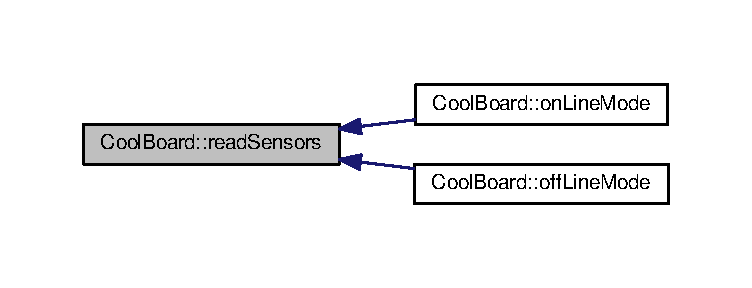
\includegraphics[width=350pt]{d7/df9/class_cool_board_ad03abdce2e65f520bbf2cff0f2d083cf_icgraph}
\end{center}
\end{figure}
\mbox{\Hypertarget{class_cool_board_a069952cdcb2e7f68518aa429eceadb6e}\label{class_cool_board_a069952cdcb2e7f68518aa429eceadb6e}} 
\index{Cool\+Board@{Cool\+Board}!sleep@{sleep}}
\index{sleep@{sleep}!Cool\+Board@{Cool\+Board}}
\subsubsection{\texorpdfstring{sleep()}{sleep()}}
{\footnotesize\ttfamily void Cool\+Board\+::sleep (\begin{DoxyParamCaption}\item[{unsigned long}]{interval }\end{DoxyParamCaption})}

Cool\+Board\+::sleep(int interval)\+: This method is provided to allow the board to enter deep\+Sleep mode for a period of time equal to interval in s 

Definition at line 1293 of file Cool\+Board.\+cpp.


\begin{DoxyCode}
1294 \{
1295 
1296     Serial.println( F(\textcolor{stringliteral}{"Entering CoolBoard.sleep() "}) );
1297     Serial.print( F(\textcolor{stringliteral}{"going to sleep for "}) );
1298     Serial.print(interval);
1299     Serial.println(F(\textcolor{stringliteral}{"s"}) );
1300     Serial.println();
1301     
1302     \textcolor{comment}{//interval is in seconds , interval*1000*1000 in µS}
1303     ESP.deepSleep ( ( interval * 1000 * 1000 ), WAKE\_RF\_DEFAULT) ;
1304 
1305 \}
\end{DoxyCode}
Here is the caller graph for this function\+:
\nopagebreak
\begin{figure}[H]
\begin{center}
\leavevmode
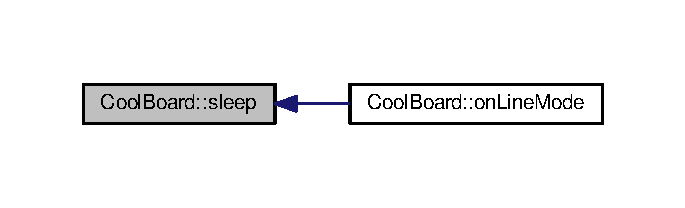
\includegraphics[width=329pt]{d7/df9/class_cool_board_a069952cdcb2e7f68518aa429eceadb6e_icgraph}
\end{center}
\end{figure}
\mbox{\Hypertarget{class_cool_board_a8612756d3f73198cdde857a66f0fe690}\label{class_cool_board_a8612756d3f73198cdde857a66f0fe690}} 
\index{Cool\+Board@{Cool\+Board}!update@{update}}
\index{update@{update}!Cool\+Board@{Cool\+Board}}
\subsubsection{\texorpdfstring{update()}{update()}}
{\footnotesize\ttfamily void Cool\+Board\+::update (\begin{DoxyParamCaption}\item[{const char $\ast$}]{answer }\end{DoxyParamCaption})}

Cool\+Board\+::update(mqtt answer)\+: This method is provided to handle the configuration update of the different parts 

Definition at line 943 of file Cool\+Board.\+cpp.


\begin{DoxyCode}
944 \{
945     \hyperlink{class_cool_board_a1b1d3c684a5baa56b08486e192fd8e97}{coolBoardLed}.\hyperlink{class_cool_board_led_ab778f5e7bed0ab74e3906d82110493c3}{fadeIn}(153,76,0,0.5);\textcolor{comment}{//shade of brown        }
946 
947 \textcolor{preprocessor}{#if DEBUG == 1}
948 
949     Serial.println( F(\textcolor{stringliteral}{"Entering CoolBoard.update() "}) );
950     Serial.println();
951     Serial.println( F(\textcolor{stringliteral}{"message is : "}) );
952     Serial.println(\hyperlink{class_cool_board_a7b835fafd449e5282f7f91d787a2dc15}{answer});
953     Serial.println();
954 
955 \textcolor{preprocessor}{#endif}
956 
957     DynamicJsonBuffer jsonBuffer;
958     JsonObject & root = jsonBuffer.parseObject(\hyperlink{class_cool_board_a7b835fafd449e5282f7f91d787a2dc15}{answer});
959     JsonObject & stateDesired = root[\textcolor{stringliteral}{"state"}];
960 
961 \textcolor{preprocessor}{#if DEBUG == 1}
962 
963     Serial.println( F(\textcolor{stringliteral}{"root json : "}) );
964     root.printTo(Serial);
965     Serial.println();
966 
967     Serial.println( F(\textcolor{stringliteral}{"stateDesired json : "}));
968     stateDesired.printTo(Serial);
969     Serial.println();
970     
971     Serial.print( F(\textcolor{stringliteral}{"jsonBuffer size : "}));
972     Serial.println(jsonBuffer.size());
973 
974 \textcolor{preprocessor}{#endif}
975 
976     \textcolor{keywordflow}{if} (stateDesired.success())
977     \{
978     
979 \textcolor{preprocessor}{    #if DEBUG == 1}
980 
981         Serial.println( F(\textcolor{stringliteral}{"update message parsing : success"}) );
982         Serial.println();
983     
984 \textcolor{preprocessor}{    #endif}
985 
986             String answerDesired;
987         
988             stateDesired.printTo(answerDesired);
989             
990 \textcolor{preprocessor}{        #if DEBUG == 1      }
991         
992             Serial.println( F(\textcolor{stringliteral}{"update is ok "}) );
993             Serial.println( F(\textcolor{stringliteral}{"desired update is : "}) );            
994             Serial.println(answerDesired);
995             Serial.println(\textcolor{stringliteral}{"json size is : "});
996             Serial.println(jsonBuffer.size() ) ;                
997             Serial.println();
998 
999         
1000 \textcolor{preprocessor}{        #endif}
1001             \textcolor{comment}{//manual mode check}
1002             \textcolor{keywordflow}{if}(this->\hyperlink{class_cool_board_a7c8e505a5804b109e112d5a03df6ea2b}{manual} == 1 )
1003             \{ 
1004                 JsonObject & manualMode=stateDesired[\textcolor{stringliteral}{"manual"}];
1005                 \textcolor{comment}{//json parse}
1006                 \textcolor{keywordflow}{for}(\textcolor{keyword}{auto} kv : manualMode)
1007                 \{
1008 \textcolor{preprocessor}{                #if DEBUG == 1}
1009 
1010                     Serial.print(F(\textcolor{stringliteral}{"writing to "}));
1011                     Serial.println(kv.key);
1012                     Serial.print(F(\textcolor{stringliteral}{"state : "}));
1013                     Serial.println(kv.value.as<\textcolor{keywordtype}{bool}>());        
1014                     
1015 \textcolor{preprocessor}{                #endif              }
1016 
1017                     \textcolor{keywordflow}{if}( strcmp(kv.key,\textcolor{stringliteral}{"Act0"}) == 0 )
1018                     \{
1019                     
1020                         \hyperlink{class_cool_board_a30b1357881b01ccbec676856a91e48e9}{jetPack}.\hyperlink{class_jetpack_a79ae7bc3c1828a0551a7c005c4f8bd00}{writeBit}(0,kv.value.as<\textcolor{keywordtype}{bool}>() ); 
1021                         
1022                     \}
1023                     \textcolor{keywordflow}{else} \textcolor{keywordflow}{if}(strcmp(kv.key,\textcolor{stringliteral}{"Act1"}) == 0)
1024                     \{
1025                         \hyperlink{class_cool_board_a30b1357881b01ccbec676856a91e48e9}{jetPack}.\hyperlink{class_jetpack_a79ae7bc3c1828a0551a7c005c4f8bd00}{writeBit}(1,kv.value.as<\textcolor{keywordtype}{bool}>() ); 
1026 
1027                     \}
1028                     \textcolor{keywordflow}{else} \textcolor{keywordflow}{if}(strcmp(kv.key,\textcolor{stringliteral}{"Act2"}) == 0)
1029                     \{
1030                         \hyperlink{class_cool_board_a30b1357881b01ccbec676856a91e48e9}{jetPack}.\hyperlink{class_jetpack_a79ae7bc3c1828a0551a7c005c4f8bd00}{writeBit}(2,kv.value.as<\textcolor{keywordtype}{bool}>() ); 
1031 
1032                     \}
1033                     \textcolor{keywordflow}{else} \textcolor{keywordflow}{if}(strcmp(kv.key,\textcolor{stringliteral}{"Act3"}) == 0)
1034                     \{
1035                         \hyperlink{class_cool_board_a30b1357881b01ccbec676856a91e48e9}{jetPack}.\hyperlink{class_jetpack_a79ae7bc3c1828a0551a7c005c4f8bd00}{writeBit}(3,kv.value.as<\textcolor{keywordtype}{bool}>() ); 
1036 
1037                     \}
1038                     \textcolor{keywordflow}{else} \textcolor{keywordflow}{if}(strcmp(kv.key,\textcolor{stringliteral}{"Act4"}) == 0)
1039                     \{
1040                         \hyperlink{class_cool_board_a30b1357881b01ccbec676856a91e48e9}{jetPack}.\hyperlink{class_jetpack_a79ae7bc3c1828a0551a7c005c4f8bd00}{writeBit}(4,kv.value.as<\textcolor{keywordtype}{bool}>() ); 
1041 
1042                     \}
1043                     \textcolor{keywordflow}{else} \textcolor{keywordflow}{if}(strcmp(kv.key,\textcolor{stringliteral}{"Act5"}) == 0)
1044                     \{
1045                         \hyperlink{class_cool_board_a30b1357881b01ccbec676856a91e48e9}{jetPack}.\hyperlink{class_jetpack_a79ae7bc3c1828a0551a7c005c4f8bd00}{writeBit}(5,kv.value.as<\textcolor{keywordtype}{bool}>() ); 
1046 
1047                     \}
1048                     \textcolor{keywordflow}{else} \textcolor{keywordflow}{if}(strcmp(kv.key,\textcolor{stringliteral}{"Act6"}) == 0)
1049                     \{
1050                         \hyperlink{class_cool_board_a30b1357881b01ccbec676856a91e48e9}{jetPack}.\hyperlink{class_jetpack_a79ae7bc3c1828a0551a7c005c4f8bd00}{writeBit}(6,kv.value.as<\textcolor{keywordtype}{bool}>() ); 
1051 
1052                     \}
1053                     \textcolor{keywordflow}{else} \textcolor{keywordflow}{if} (strcmp(kv.key,\textcolor{stringliteral}{"Act7"}) == 0)
1054                     \{
1055                         \hyperlink{class_cool_board_a30b1357881b01ccbec676856a91e48e9}{jetPack}.\hyperlink{class_jetpack_a79ae7bc3c1828a0551a7c005c4f8bd00}{writeBit}(7,kv.value.as<\textcolor{keywordtype}{bool}>() ); 
1056 
1057                     \}
1058                     \textcolor{keywordflow}{else} \textcolor{keywordflow}{if} (strcmp(kv.key,\textcolor{stringliteral}{"ActB"}) == 0)
1059                     \{
1060                         \hyperlink{class_cool_board_a4ac693895c21025b8808653f2a4316e6}{onBoardActor}.\hyperlink{class_cool_board_actor_a958786ff01ea1056ee72c72d439f86da}{write}(kv.value.as<\textcolor{keywordtype}{bool}>() ); 
1061 
1062                     \}
1063                                 
1064                 
1065                 \}
1066 
1067                 
1068             \}
1069 
1070             \textcolor{comment}{//saving the new configuration}
1071             \hyperlink{class_cool_board_a42c2586fbb13ff7f06538e9284e8538d}{fileSystem}.\hyperlink{class_cool_file_system_adfa8e2e80641ae6f0cceabd348a9b841}{updateConfigFiles}(answerDesired);
1072 
1073                 \textcolor{comment}{//answering the update msg:}
1074             \textcolor{comment}{//reported = received configuration}
1075             \textcolor{comment}{//desired=null}
1076         
1077             String updateAnswer;
1078             String tempString;
1079             
1080             stateDesired.printTo(tempString);
1081             updateAnswer=\textcolor{stringliteral}{"\{\(\backslash\)"state\(\backslash\)":\{\(\backslash\)"reported\(\backslash\)":"};
1082             updateAnswer+=tempString;
1083             updateAnswer+=\textcolor{stringliteral}{",\(\backslash\)"desired\(\backslash\)":null\}\}"};
1084 
1085 \textcolor{preprocessor}{        #if DEBUG == 1}
1086 
1087             Serial.println( F(\textcolor{stringliteral}{"preparing answer message "}) );
1088             Serial.println();
1089             Serial.println( F(\textcolor{stringliteral}{"updateAnswer : "}) );
1090             Serial.println(updateAnswer);
1091         
1092 \textcolor{preprocessor}{        #endif  }
1093 
1094             \hyperlink{class_cool_board_a2399f44d7c23c1149a335cb3b46d90f1}{mqtt}.\hyperlink{class_cool_m_q_t_t_ace977b3e90ab14b1199fe5c4fb0a13ec}{publish}(updateAnswer.c\_str());
1095             
1096             \hyperlink{class_cool_board_a2399f44d7c23c1149a335cb3b46d90f1}{mqtt}.\hyperlink{class_cool_m_q_t_t_aa5eaae967b562b62cbcf2b8d81f6e5d5}{mqttLoop}();
1097 
1098             delay(10);
1099         
1100             \textcolor{keywordflow}{if}(\hyperlink{class_cool_board_a7c8e505a5804b109e112d5a03df6ea2b}{manual} == 0 )
1101             \{
1102                 \textcolor{comment}{//restart the esp to apply the config}
1103                 ESP.restart();
1104             \}
1105     \}
1106     \textcolor{keywordflow}{else}
1107     \{
1108     
1109 \textcolor{preprocessor}{    #if DEBUG == 1}
1110 
1111         Serial.println( F(\textcolor{stringliteral}{"Failed to parse update message( OR no message received )"}) );
1112         Serial.println();
1113     
1114 \textcolor{preprocessor}{    #endif}
1115     
1116     \}
1117 
1118     \hyperlink{class_cool_board_a1b1d3c684a5baa56b08486e192fd8e97}{coolBoardLed}.\hyperlink{class_cool_board_led_ad5f0de4c628cbfbf49896042831c64ad}{strobe}(153,76,0,0.5);\textcolor{comment}{//shade of brown}
1119     \hyperlink{class_cool_board_a1b1d3c684a5baa56b08486e192fd8e97}{coolBoardLed}.\hyperlink{class_cool_board_led_a93d545679237e8cc858324367149775c}{fadeOut}(153,76,0,0.5);\textcolor{comment}{//shade of brown                              }
1120 \}
\end{DoxyCode}
Here is the call graph for this function\+:
\nopagebreak
\begin{figure}[H]
\begin{center}
\leavevmode
\includegraphics[width=350pt]{d7/df9/class_cool_board_a8612756d3f73198cdde857a66f0fe690_cgraph}
\end{center}
\end{figure}
Here is the caller graph for this function\+:
\nopagebreak
\begin{figure}[H]
\begin{center}
\leavevmode
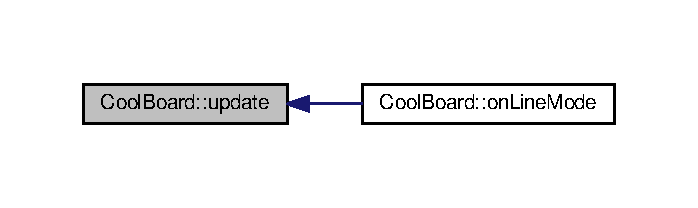
\includegraphics[width=335pt]{d7/df9/class_cool_board_a8612756d3f73198cdde857a66f0fe690_icgraph}
\end{center}
\end{figure}
\mbox{\Hypertarget{class_cool_board_ae7358fb6e623cfc81b775f5f1734909b}\label{class_cool_board_ae7358fb6e623cfc81b775f5f1734909b}} 
\index{Cool\+Board@{Cool\+Board}!user\+Data@{user\+Data}}
\index{user\+Data@{user\+Data}!Cool\+Board@{Cool\+Board}}
\subsubsection{\texorpdfstring{user\+Data()}{userData()}}
{\footnotesize\ttfamily String Cool\+Board\+::user\+Data (\begin{DoxyParamCaption}{ }\end{DoxyParamCaption})}

\hyperlink{class_cool_board_ae7358fb6e623cfc81b775f5f1734909b}{Cool\+Board\+::user\+Data()}\+: This method is provided to return the user\textquotesingle{}s data.

\begin{DoxyReturn}{Returns}
json string of the user\textquotesingle{}s data 
\end{DoxyReturn}


Definition at line 1246 of file Cool\+Board.\+cpp.


\begin{DoxyCode}
1247 \{
1248 
1249 \textcolor{preprocessor}{#if DEBUG == 1}
1250 
1251     Serial.println( F(\textcolor{stringliteral}{"Entering CoolBoard.userData() "}) );
1252     Serial.println();
1253 
1254 \textcolor{preprocessor}{#endif}
1255 
1256     String tempMAC = WiFi.macAddress();
1257 
1258     tempMAC.replace(\textcolor{stringliteral}{":"}, \textcolor{stringliteral}{""});
1259 
1260     String userJson = \textcolor{stringliteral}{"\{\(\backslash\)"user\(\backslash\)":\(\backslash\)""};
1261 
1262     userJson += \hyperlink{class_cool_board_a2399f44d7c23c1149a335cb3b46d90f1}{mqtt}.\hyperlink{class_cool_m_q_t_t_a373cc92fca7760d886f02d8a6e5b3f63}{getUser}();
1263 
1264     userJson += \textcolor{stringliteral}{"\(\backslash\)",\(\backslash\)"timestamp\(\backslash\)":\(\backslash\)""};
1265 
1266     userJson += \hyperlink{class_cool_board_a50d2a6716879d64a85f3c6b44ad63275}{rtc}.\hyperlink{class_cool_time_ac4f32ee513c1328d984306645e8785a4}{getESDate}(); \textcolor{comment}{// "timestamp":"20yy-mm-ddThh:mm:ssZ"}
1267 
1268     userJson += \textcolor{stringliteral}{"\(\backslash\)",\(\backslash\)"mac\(\backslash\)":\(\backslash\)""};
1269 
1270     userJson += tempMAC;
1271 
1272     userJson += \textcolor{stringliteral}{"\(\backslash\)"\}"};
1273 
1274 \textcolor{preprocessor}{#if DEBUG == 1}
1275 
1276     Serial.println( F(\textcolor{stringliteral}{"userData is : "}) );
1277     Serial.println(userJson);
1278     Serial.println();
1279 
1280 \textcolor{preprocessor}{#endif  }
1281     
1282     \textcolor{keywordflow}{return}(userJson);
1283     
1284 \}
\end{DoxyCode}
Here is the call graph for this function\+:
\nopagebreak
\begin{figure}[H]
\begin{center}
\leavevmode
\includegraphics[width=350pt]{d7/df9/class_cool_board_ae7358fb6e623cfc81b775f5f1734909b_cgraph}
\end{center}
\end{figure}
Here is the caller graph for this function\+:
\nopagebreak
\begin{figure}[H]
\begin{center}
\leavevmode
\includegraphics[width=346pt]{d7/df9/class_cool_board_ae7358fb6e623cfc81b775f5f1734909b_icgraph}
\end{center}
\end{figure}


\subsection{Member Data Documentation}
\mbox{\Hypertarget{class_cool_board_a7b835fafd449e5282f7f91d787a2dc15}\label{class_cool_board_a7b835fafd449e5282f7f91d787a2dc15}} 
\index{Cool\+Board@{Cool\+Board}!answer@{answer}}
\index{answer@{answer}!Cool\+Board@{Cool\+Board}}
\subsubsection{\texorpdfstring{answer}{answer}}
{\footnotesize\ttfamily String Cool\+Board\+::answer =\char`\"{}\char`\"{}\hspace{0.3cm}{\ttfamily [private]}}



Definition at line 106 of file Cool\+Board.\+h.

\mbox{\Hypertarget{class_cool_board_a1b1d3c684a5baa56b08486e192fd8e97}\label{class_cool_board_a1b1d3c684a5baa56b08486e192fd8e97}} 
\index{Cool\+Board@{Cool\+Board}!cool\+Board\+Led@{cool\+Board\+Led}}
\index{cool\+Board\+Led@{cool\+Board\+Led}!Cool\+Board@{Cool\+Board}}
\subsubsection{\texorpdfstring{cool\+Board\+Led}{coolBoardLed}}
{\footnotesize\ttfamily \hyperlink{class_cool_board_led}{Cool\+Board\+Led} Cool\+Board\+::cool\+Board\+Led\hspace{0.3cm}{\ttfamily [private]}}



Definition at line 74 of file Cool\+Board.\+h.

\mbox{\Hypertarget{class_cool_board_af102be5288bd7f7a8e59b13f86e26a00}\label{class_cool_board_af102be5288bd7f7a8e59b13f86e26a00}} 
\index{Cool\+Board@{Cool\+Board}!cool\+Board\+Sensors@{cool\+Board\+Sensors}}
\index{cool\+Board\+Sensors@{cool\+Board\+Sensors}!Cool\+Board@{Cool\+Board}}
\subsubsection{\texorpdfstring{cool\+Board\+Sensors}{coolBoardSensors}}
{\footnotesize\ttfamily \hyperlink{class_cool_board_sensors}{Cool\+Board\+Sensors} Cool\+Board\+::cool\+Board\+Sensors\hspace{0.3cm}{\ttfamily [private]}}



Definition at line 72 of file Cool\+Board.\+h.

\mbox{\Hypertarget{class_cool_board_a427fb753dd8575bdf821c70a5c63d695}\label{class_cool_board_a427fb753dd8575bdf821c70a5c63d695}} 
\index{Cool\+Board@{Cool\+Board}!data@{data}}
\index{data@{data}!Cool\+Board@{Cool\+Board}}
\subsubsection{\texorpdfstring{data}{data}}
{\footnotesize\ttfamily String Cool\+Board\+::data =\char`\"{}\char`\"{}\hspace{0.3cm}{\ttfamily [private]}}



Definition at line 104 of file Cool\+Board.\+h.

\mbox{\Hypertarget{class_cool_board_af1fe1376fc66f93dee80b327ca695377}\label{class_cool_board_af1fe1376fc66f93dee80b327ca695377}} 
\index{Cool\+Board@{Cool\+Board}!En\+I2C@{En\+I2C}}
\index{En\+I2C@{En\+I2C}!Cool\+Board@{Cool\+Board}}
\subsubsection{\texorpdfstring{En\+I2C}{EnI2C}}
{\footnotesize\ttfamily const int Cool\+Board\+::\+En\+I2C = 5\hspace{0.3cm}{\ttfamily [private]}}



Definition at line 108 of file Cool\+Board.\+h.

\mbox{\Hypertarget{class_cool_board_a09e26264839c65873eb56af476eff6b2}\label{class_cool_board_a09e26264839c65873eb56af476eff6b2}} 
\index{Cool\+Board@{Cool\+Board}!external\+Sensors@{external\+Sensors}}
\index{external\+Sensors@{external\+Sensors}!Cool\+Board@{Cool\+Board}}
\subsubsection{\texorpdfstring{external\+Sensors}{externalSensors}}
{\footnotesize\ttfamily \hyperlink{class_external_sensors}{External\+Sensors} Cool\+Board\+::external\+Sensors\hspace{0.3cm}{\ttfamily [private]}}



Definition at line 86 of file Cool\+Board.\+h.

\mbox{\Hypertarget{class_cool_board_a638b00b76aeb819ecfd4c10b8cdd7bb7}\label{class_cool_board_a638b00b76aeb819ecfd4c10b8cdd7bb7}} 
\index{Cool\+Board@{Cool\+Board}!external\+Sensors\+Active@{external\+Sensors\+Active}}
\index{external\+Sensors\+Active@{external\+Sensors\+Active}!Cool\+Board@{Cool\+Board}}
\subsubsection{\texorpdfstring{external\+Sensors\+Active}{externalSensorsActive}}
{\footnotesize\ttfamily bool Cool\+Board\+::external\+Sensors\+Active =0\hspace{0.3cm}{\ttfamily [private]}}



Definition at line 96 of file Cool\+Board.\+h.

\mbox{\Hypertarget{class_cool_board_a42c2586fbb13ff7f06538e9284e8538d}\label{class_cool_board_a42c2586fbb13ff7f06538e9284e8538d}} 
\index{Cool\+Board@{Cool\+Board}!file\+System@{file\+System}}
\index{file\+System@{file\+System}!Cool\+Board@{Cool\+Board}}
\subsubsection{\texorpdfstring{file\+System}{fileSystem}}
{\footnotesize\ttfamily \hyperlink{class_cool_file_system}{Cool\+File\+System} Cool\+Board\+::file\+System\hspace{0.3cm}{\ttfamily [private]}}



Definition at line 70 of file Cool\+Board.\+h.

\mbox{\Hypertarget{class_cool_board_ad103718ce316006c4695b8eb312eaf11}\label{class_cool_board_ad103718ce316006c4695b8eb312eaf11}} 
\index{Cool\+Board@{Cool\+Board}!irene3000@{irene3000}}
\index{irene3000@{irene3000}!Cool\+Board@{Cool\+Board}}
\subsubsection{\texorpdfstring{irene3000}{irene3000}}
{\footnotesize\ttfamily \hyperlink{class_irene3000}{Irene3000} Cool\+Board\+::irene3000\hspace{0.3cm}{\ttfamily [private]}}



Definition at line 84 of file Cool\+Board.\+h.

\mbox{\Hypertarget{class_cool_board_a9c3f7ac625481ee2ae802a25d97a4ae0}\label{class_cool_board_a9c3f7ac625481ee2ae802a25d97a4ae0}} 
\index{Cool\+Board@{Cool\+Board}!irene\+Active@{irene\+Active}}
\index{irene\+Active@{irene\+Active}!Cool\+Board@{Cool\+Board}}
\subsubsection{\texorpdfstring{irene\+Active}{ireneActive}}
{\footnotesize\ttfamily bool Cool\+Board\+::irene\+Active =0\hspace{0.3cm}{\ttfamily [private]}}



Definition at line 92 of file Cool\+Board.\+h.

\mbox{\Hypertarget{class_cool_board_a30b1357881b01ccbec676856a91e48e9}\label{class_cool_board_a30b1357881b01ccbec676856a91e48e9}} 
\index{Cool\+Board@{Cool\+Board}!jet\+Pack@{jet\+Pack}}
\index{jet\+Pack@{jet\+Pack}!Cool\+Board@{Cool\+Board}}
\subsubsection{\texorpdfstring{jet\+Pack}{jetPack}}
{\footnotesize\ttfamily \hyperlink{class_jetpack}{Jetpack} Cool\+Board\+::jet\+Pack\hspace{0.3cm}{\ttfamily [private]}}



Definition at line 82 of file Cool\+Board.\+h.

\mbox{\Hypertarget{class_cool_board_a9be03a913d26e558328935ca3b59a75e}\label{class_cool_board_a9be03a913d26e558328935ca3b59a75e}} 
\index{Cool\+Board@{Cool\+Board}!jetpack\+Active@{jetpack\+Active}}
\index{jetpack\+Active@{jetpack\+Active}!Cool\+Board@{Cool\+Board}}
\subsubsection{\texorpdfstring{jetpack\+Active}{jetpackActive}}
{\footnotesize\ttfamily bool Cool\+Board\+::jetpack\+Active =0\hspace{0.3cm}{\ttfamily [private]}}



Definition at line 94 of file Cool\+Board.\+h.

\mbox{\Hypertarget{class_cool_board_a84bc94413b64973e4aba8c467c97006c}\label{class_cool_board_a84bc94413b64973e4aba8c467c97006c}} 
\index{Cool\+Board@{Cool\+Board}!log\+Interval@{log\+Interval}}
\index{log\+Interval@{log\+Interval}!Cool\+Board@{Cool\+Board}}
\subsubsection{\texorpdfstring{log\+Interval}{logInterval}}
{\footnotesize\ttfamily unsigned long Cool\+Board\+::log\+Interval =1\hspace{0.3cm}{\ttfamily [private]}}



Definition at line 102 of file Cool\+Board.\+h.

\mbox{\Hypertarget{class_cool_board_a7c8e505a5804b109e112d5a03df6ea2b}\label{class_cool_board_a7c8e505a5804b109e112d5a03df6ea2b}} 
\index{Cool\+Board@{Cool\+Board}!manual@{manual}}
\index{manual@{manual}!Cool\+Board@{Cool\+Board}}
\subsubsection{\texorpdfstring{manual}{manual}}
{\footnotesize\ttfamily bool Cool\+Board\+::manual =0\hspace{0.3cm}{\ttfamily [private]}}



Definition at line 100 of file Cool\+Board.\+h.

\mbox{\Hypertarget{class_cool_board_a2399f44d7c23c1149a335cb3b46d90f1}\label{class_cool_board_a2399f44d7c23c1149a335cb3b46d90f1}} 
\index{Cool\+Board@{Cool\+Board}!mqtt@{mqtt}}
\index{mqtt@{mqtt}!Cool\+Board@{Cool\+Board}}
\subsubsection{\texorpdfstring{mqtt}{mqtt}}
{\footnotesize\ttfamily \hyperlink{class_cool_m_q_t_t}{Cool\+M\+Q\+TT} Cool\+Board\+::mqtt\hspace{0.3cm}{\ttfamily [private]}}



Definition at line 80 of file Cool\+Board.\+h.

\mbox{\Hypertarget{class_cool_board_a4ac693895c21025b8808653f2a4316e6}\label{class_cool_board_a4ac693895c21025b8808653f2a4316e6}} 
\index{Cool\+Board@{Cool\+Board}!on\+Board\+Actor@{on\+Board\+Actor}}
\index{on\+Board\+Actor@{on\+Board\+Actor}!Cool\+Board@{Cool\+Board}}
\subsubsection{\texorpdfstring{on\+Board\+Actor}{onBoardActor}}
{\footnotesize\ttfamily \hyperlink{class_cool_board_actor}{Cool\+Board\+Actor} Cool\+Board\+::on\+Board\+Actor\hspace{0.3cm}{\ttfamily [private]}}



Definition at line 88 of file Cool\+Board.\+h.

\mbox{\Hypertarget{class_cool_board_a50d2a6716879d64a85f3c6b44ad63275}\label{class_cool_board_a50d2a6716879d64a85f3c6b44ad63275}} 
\index{Cool\+Board@{Cool\+Board}!rtc@{rtc}}
\index{rtc@{rtc}!Cool\+Board@{Cool\+Board}}
\subsubsection{\texorpdfstring{rtc}{rtc}}
{\footnotesize\ttfamily \hyperlink{class_cool_time}{Cool\+Time} Cool\+Board\+::rtc\hspace{0.3cm}{\ttfamily [private]}}



Definition at line 76 of file Cool\+Board.\+h.

\mbox{\Hypertarget{class_cool_board_a0a51b2287139f66c738101fb53139230}\label{class_cool_board_a0a51b2287139f66c738101fb53139230}} 
\index{Cool\+Board@{Cool\+Board}!sleep\+Active@{sleep\+Active}}
\index{sleep\+Active@{sleep\+Active}!Cool\+Board@{Cool\+Board}}
\subsubsection{\texorpdfstring{sleep\+Active}{sleepActive}}
{\footnotesize\ttfamily bool Cool\+Board\+::sleep\+Active =0\hspace{0.3cm}{\ttfamily [private]}}



Definition at line 98 of file Cool\+Board.\+h.

\mbox{\Hypertarget{class_cool_board_a6395459131d6889a3005f79c7a35e964}\label{class_cool_board_a6395459131d6889a3005f79c7a35e964}} 
\index{Cool\+Board@{Cool\+Board}!user\+Active@{user\+Active}}
\index{user\+Active@{user\+Active}!Cool\+Board@{Cool\+Board}}
\subsubsection{\texorpdfstring{user\+Active}{userActive}}
{\footnotesize\ttfamily bool Cool\+Board\+::user\+Active =0\hspace{0.3cm}{\ttfamily [private]}}



Definition at line 90 of file Cool\+Board.\+h.

\mbox{\Hypertarget{class_cool_board_acd88e6003606b47479ebba81e4aceeca}\label{class_cool_board_acd88e6003606b47479ebba81e4aceeca}} 
\index{Cool\+Board@{Cool\+Board}!wifi\+Manager@{wifi\+Manager}}
\index{wifi\+Manager@{wifi\+Manager}!Cool\+Board@{Cool\+Board}}
\subsubsection{\texorpdfstring{wifi\+Manager}{wifiManager}}
{\footnotesize\ttfamily \hyperlink{class_cool_wifi}{Cool\+Wifi} Cool\+Board\+::wifi\+Manager\hspace{0.3cm}{\ttfamily [private]}}



Definition at line 78 of file Cool\+Board.\+h.



The documentation for this class was generated from the following files\+:\begin{DoxyCompactItemize}
\item 
/home/ashiroji/\+Arduino/libraries/\+Cool\+Board/src/\hyperlink{_cool_board_8h}{Cool\+Board.\+h}\item 
/home/ashiroji/\+Arduino/libraries/\+Cool\+Board/src/\hyperlink{_cool_board_8cpp}{Cool\+Board.\+cpp}\end{DoxyCompactItemize}

\hypertarget{class_cool_board_led}{}\section{Cool\+Board\+Led Class Reference}
\label{class_cool_board_led}\index{Cool\+Board\+Led@{Cool\+Board\+Led}}


This class handles the led in the Sensor Board.  




{\ttfamily \#include $<$Cool\+Board\+Led.\+h$>$}



Collaboration diagram for Cool\+Board\+Led\+:\nopagebreak
\begin{figure}[H]
\begin{center}
\leavevmode
\includegraphics[width=158pt]{d4/d22/class_cool_board_led__coll__graph}
\end{center}
\end{figure}
\subsection*{Public Member Functions}
\begin{DoxyCompactItemize}
\item 
void \hyperlink{class_cool_board_led_ae3cbde8affcc6f011cbd698c8ef911f6}{begin} ()
\item 
void \hyperlink{class_cool_board_led_a30fadd4cbec17ceea428bf7a32207e87}{write} (int R, int G, int B)
\item 
void \hyperlink{class_cool_board_led_a69f323359e0c9f797422f2152b5d41ef}{end} ()
\item 
bool \hyperlink{class_cool_board_led_a1b60e5e30bea96c49ed62ed1bf1ffc8b}{config} ()
\item 
void \hyperlink{class_cool_board_led_ae74fe4b47d06c3a97b468ba220c4eb99}{activate} ()
\item 
void \hyperlink{class_cool_board_led_a8ed3053a36f0ed4a131f43b5b17efb61}{print\+Conf} ()
\item 
void \hyperlink{class_cool_board_led_af1cacbaa88db8bcf6042c1083ba41155}{fade} (int R, int G, int B, float T)
\item 
void \hyperlink{class_cool_board_led_a96e1ea13003eee34c9dbcef340404426}{blink} (int R, int G, int B, float T)
\item 
void \hyperlink{class_cool_board_led_ab778f5e7bed0ab74e3906d82110493c3}{fade\+In} (int R, int G, int B, float T)
\item 
void \hyperlink{class_cool_board_led_a93d545679237e8cc858324367149775c}{fade\+Out} (int R, int G, int B, float T)
\item 
void \hyperlink{class_cool_board_led_ad5f0de4c628cbfbf49896042831c64ad}{strobe} (int R, int G, int B, float T)
\end{DoxyCompactItemize}
\subsection*{Private Attributes}
\begin{DoxyCompactItemize}
\item 
Neo\+Pixel\+Bus$<$ Neo\+Grb\+Feature, Neo800\+Kbps\+Method $>$ $\ast$ \hyperlink{class_cool_board_led_ac2c13fa462a010cd9242bf297c013923}{neo\+Pixel\+Led} = N\+U\+LL
\item 
bool \hyperlink{class_cool_board_led_aadd04d2ecf123247718d77f42fba7f08}{led\+Active} =0
\end{DoxyCompactItemize}


\subsection{Detailed Description}
This class handles the led in the Sensor Board. 

Definition at line 45 of file Cool\+Board\+Led.\+h.



\subsection{Member Function Documentation}
\mbox{\Hypertarget{class_cool_board_led_ae3cbde8affcc6f011cbd698c8ef911f6}\label{class_cool_board_led_ae3cbde8affcc6f011cbd698c8ef911f6}} 
\index{Cool\+Board\+Led@{Cool\+Board\+Led}!begin@{begin}}
\index{begin@{begin}!Cool\+Board\+Led@{Cool\+Board\+Led}}
\subsubsection{\texorpdfstring{begin()}{begin()}}
{\footnotesize\ttfamily void Cool\+Board\+Led\+::begin (\begin{DoxyParamCaption}{ }\end{DoxyParamCaption})}

\hyperlink{class_cool_board_led_ae3cbde8affcc6f011cbd698c8ef911f6}{Cool\+Board\+Led\+::begin()}\+: This method is provided to start the Led Object by setting the correct pin and creating a dynamic neo\+Pixel\+Bus 

Definition at line 249 of file Cool\+Board\+Led.\+cpp.



References led\+Active, and neo\+Pixel\+Led.



Referenced by Cool\+Board\+::config().

Here is the caller graph for this function\+:
\nopagebreak
\begin{figure}[H]
\begin{center}
\leavevmode
\includegraphics[width=318pt]{de/dc0/class_cool_board_led_ae3cbde8affcc6f011cbd698c8ef911f6_icgraph}
\end{center}
\end{figure}
\mbox{\Hypertarget{class_cool_board_led_a30fadd4cbec17ceea428bf7a32207e87}\label{class_cool_board_led_a30fadd4cbec17ceea428bf7a32207e87}} 
\index{Cool\+Board\+Led@{Cool\+Board\+Led}!write@{write}}
\index{write@{write}!Cool\+Board\+Led@{Cool\+Board\+Led}}
\subsubsection{\texorpdfstring{write()}{write()}}
{\footnotesize\ttfamily void Cool\+Board\+Led\+::write (\begin{DoxyParamCaption}\item[{int}]{R,  }\item[{int}]{G,  }\item[{int}]{B }\end{DoxyParamCaption})}

Cool\+Board\+Led\+::write(\+Red,\+Green,\+Blue)\+: This method is provided to set the Color of the Led 

Definition at line 275 of file Cool\+Board\+Led.\+cpp.



References led\+Active, and neo\+Pixel\+Led.



Referenced by Cool\+Board\+::begin(), and Cool\+Board\+::connect().

Here is the caller graph for this function\+:
\nopagebreak
\begin{figure}[H]
\begin{center}
\leavevmode
\includegraphics[width=350pt]{de/dc0/class_cool_board_led_a30fadd4cbec17ceea428bf7a32207e87_icgraph}
\end{center}
\end{figure}
\mbox{\Hypertarget{class_cool_board_led_a69f323359e0c9f797422f2152b5d41ef}\label{class_cool_board_led_a69f323359e0c9f797422f2152b5d41ef}} 
\index{Cool\+Board\+Led@{Cool\+Board\+Led}!end@{end}}
\index{end@{end}!Cool\+Board\+Led@{Cool\+Board\+Led}}
\subsubsection{\texorpdfstring{end()}{end()}}
{\footnotesize\ttfamily void Cool\+Board\+Led\+::end (\begin{DoxyParamCaption}{ }\end{DoxyParamCaption})}

\hyperlink{class_cool_board_led_a69f323359e0c9f797422f2152b5d41ef}{Cool\+Board\+Led\+::end()} \+: this method is provided to delete the dynamically created neo\+Pixel\+Led 

Definition at line 230 of file Cool\+Board\+Led.\+cpp.



References neo\+Pixel\+Led.

\mbox{\Hypertarget{class_cool_board_led_a1b60e5e30bea96c49ed62ed1bf1ffc8b}\label{class_cool_board_led_a1b60e5e30bea96c49ed62ed1bf1ffc8b}} 
\index{Cool\+Board\+Led@{Cool\+Board\+Led}!config@{config}}
\index{config@{config}!Cool\+Board\+Led@{Cool\+Board\+Led}}
\subsubsection{\texorpdfstring{config()}{config()}}
{\footnotesize\ttfamily bool Cool\+Board\+Led\+::config (\begin{DoxyParamCaption}{ }\end{DoxyParamCaption})}

\hyperlink{class_cool_board_led_a1b60e5e30bea96c49ed62ed1bf1ffc8b}{Cool\+Board\+Led\+::config()}\+: This method is provided to configure the Led Object \+: -\/led\+Active=0 \+: deactivated -\/led\+Active=1 \+: activated \begin{DoxyReturn}{Returns}
true if the configuration done, false otherwise 
\end{DoxyReturn}


Definition at line 308 of file Cool\+Board\+Led.\+cpp.



References led\+Active.



Referenced by Cool\+Board\+::config().

Here is the caller graph for this function\+:
\nopagebreak
\begin{figure}[H]
\begin{center}
\leavevmode
\includegraphics[width=321pt]{de/dc0/class_cool_board_led_a1b60e5e30bea96c49ed62ed1bf1ffc8b_icgraph}
\end{center}
\end{figure}
\mbox{\Hypertarget{class_cool_board_led_ae74fe4b47d06c3a97b468ba220c4eb99}\label{class_cool_board_led_ae74fe4b47d06c3a97b468ba220c4eb99}} 
\index{Cool\+Board\+Led@{Cool\+Board\+Led}!activate@{activate}}
\index{activate@{activate}!Cool\+Board\+Led@{Cool\+Board\+Led}}
\subsubsection{\texorpdfstring{activate()}{activate()}}
{\footnotesize\ttfamily void Cool\+Board\+Led\+::activate (\begin{DoxyParamCaption}{ }\end{DoxyParamCaption})}

\hyperlink{class_cool_board_led_ae74fe4b47d06c3a97b468ba220c4eb99}{Cool\+Board\+Led\+::activate()}\+: This method is provided to activate the Led Object without the configuration file 

Definition at line 441 of file Cool\+Board\+Led.\+cpp.



References led\+Active.

\mbox{\Hypertarget{class_cool_board_led_a8ed3053a36f0ed4a131f43b5b17efb61}\label{class_cool_board_led_a8ed3053a36f0ed4a131f43b5b17efb61}} 
\index{Cool\+Board\+Led@{Cool\+Board\+Led}!print\+Conf@{print\+Conf}}
\index{print\+Conf@{print\+Conf}!Cool\+Board\+Led@{Cool\+Board\+Led}}
\subsubsection{\texorpdfstring{print\+Conf()}{printConf()}}
{\footnotesize\ttfamily void Cool\+Board\+Led\+::print\+Conf (\begin{DoxyParamCaption}{ }\end{DoxyParamCaption})}

\hyperlink{class_cool_board_led_a8ed3053a36f0ed4a131f43b5b17efb61}{Cool\+Board\+Led\+::print\+Conf()}\+: This method is provided to print the Led Object Configuration to the Serial Monitor 

Definition at line 417 of file Cool\+Board\+Led.\+cpp.



References led\+Active.



Referenced by Cool\+Board\+::begin().

Here is the caller graph for this function\+:
\nopagebreak
\begin{figure}[H]
\begin{center}
\leavevmode
\includegraphics[width=332pt]{de/dc0/class_cool_board_led_a8ed3053a36f0ed4a131f43b5b17efb61_icgraph}
\end{center}
\end{figure}
\mbox{\Hypertarget{class_cool_board_led_af1cacbaa88db8bcf6042c1083ba41155}\label{class_cool_board_led_af1cacbaa88db8bcf6042c1083ba41155}} 
\index{Cool\+Board\+Led@{Cool\+Board\+Led}!fade@{fade}}
\index{fade@{fade}!Cool\+Board\+Led@{Cool\+Board\+Led}}
\subsubsection{\texorpdfstring{fade()}{fade()}}
{\footnotesize\ttfamily void Cool\+Board\+Led\+::fade (\begin{DoxyParamCaption}\item[{int}]{R,  }\item[{int}]{G,  }\item[{int}]{B,  }\item[{float}]{T }\end{DoxyParamCaption})}

\hyperlink{class_cool_board_led_af1cacbaa88db8bcf6042c1083ba41155}{Cool\+Board\+Led\+::fade} ( Red , Green , Blue, Time in seconds )\+: fade animation\+: Fade In over T(seconds) Fade Out over T(seconds) 

Definition at line 50 of file Cool\+Board\+Led.\+cpp.



References led\+Active, and neo\+Pixel\+Led.



Referenced by Cool\+Board\+::off\+Line\+Mode(), and Cool\+Board\+::on\+Line\+Mode().

Here is the caller graph for this function\+:
\nopagebreak
\begin{figure}[H]
\begin{center}
\leavevmode
\includegraphics[width=341pt]{de/dc0/class_cool_board_led_af1cacbaa88db8bcf6042c1083ba41155_icgraph}
\end{center}
\end{figure}
\mbox{\Hypertarget{class_cool_board_led_a96e1ea13003eee34c9dbcef340404426}\label{class_cool_board_led_a96e1ea13003eee34c9dbcef340404426}} 
\index{Cool\+Board\+Led@{Cool\+Board\+Led}!blink@{blink}}
\index{blink@{blink}!Cool\+Board\+Led@{Cool\+Board\+Led}}
\subsubsection{\texorpdfstring{blink()}{blink()}}
{\footnotesize\ttfamily void Cool\+Board\+Led\+::blink (\begin{DoxyParamCaption}\item[{int}]{R,  }\item[{int}]{G,  }\item[{int}]{B,  }\item[{float}]{T }\end{DoxyParamCaption})}

Cool\+Board\+Led\+::blink( Red , Green , Blue , Time in seconds )\+: Blink animation\+: Led On for T seconds Led off 

Definition at line 91 of file Cool\+Board\+Led.\+cpp.



References led\+Active, and neo\+Pixel\+Led.



Referenced by Cool\+Board\+::begin(), Cool\+Board\+::config(), Cool\+Board\+::connect(), Cool\+Board\+::off\+Line\+Mode(), and Cool\+Board\+::on\+Line\+Mode().

Here is the caller graph for this function\+:
\nopagebreak
\begin{figure}[H]
\begin{center}
\leavevmode
\includegraphics[width=350pt]{de/dc0/class_cool_board_led_a96e1ea13003eee34c9dbcef340404426_icgraph}
\end{center}
\end{figure}
\mbox{\Hypertarget{class_cool_board_led_ab778f5e7bed0ab74e3906d82110493c3}\label{class_cool_board_led_ab778f5e7bed0ab74e3906d82110493c3}} 
\index{Cool\+Board\+Led@{Cool\+Board\+Led}!fade\+In@{fade\+In}}
\index{fade\+In@{fade\+In}!Cool\+Board\+Led@{Cool\+Board\+Led}}
\subsubsection{\texorpdfstring{fade\+In()}{fadeIn()}}
{\footnotesize\ttfamily void Cool\+Board\+Led\+::fade\+In (\begin{DoxyParamCaption}\item[{int}]{R,  }\item[{int}]{G,  }\item[{int}]{B,  }\item[{float}]{T }\end{DoxyParamCaption})}

Cool\+Board\+Led\+::fade\+In(\+Red , Green , Blue , Time in seconds) Fade In animation\+: gradual increase over T(seconds) 

Definition at line 124 of file Cool\+Board\+Led.\+cpp.



References led\+Active, and neo\+Pixel\+Led.



Referenced by Cool\+Board\+::config(), Cool\+Board\+::off\+Line\+Mode(), Cool\+Board\+::on\+Line\+Mode(), Cool\+Board\+::read\+Sensors(), and Cool\+Board\+::update().

Here is the caller graph for this function\+:
\nopagebreak
\begin{figure}[H]
\begin{center}
\leavevmode
\includegraphics[width=350pt]{de/dc0/class_cool_board_led_ab778f5e7bed0ab74e3906d82110493c3_icgraph}
\end{center}
\end{figure}
\mbox{\Hypertarget{class_cool_board_led_a93d545679237e8cc858324367149775c}\label{class_cool_board_led_a93d545679237e8cc858324367149775c}} 
\index{Cool\+Board\+Led@{Cool\+Board\+Led}!fade\+Out@{fade\+Out}}
\index{fade\+Out@{fade\+Out}!Cool\+Board\+Led@{Cool\+Board\+Led}}
\subsubsection{\texorpdfstring{fade\+Out()}{fadeOut()}}
{\footnotesize\ttfamily void Cool\+Board\+Led\+::fade\+Out (\begin{DoxyParamCaption}\item[{int}]{R,  }\item[{int}]{G,  }\item[{int}]{B,  }\item[{float}]{T }\end{DoxyParamCaption})}

Cool\+Board\+Led\+::fade\+Out( Red , Green , Blue , Time in seconds) Fade Out animation\+: gradual decrease over T(seconds) 

Definition at line 159 of file Cool\+Board\+Led.\+cpp.



References led\+Active, and neo\+Pixel\+Led.



Referenced by Cool\+Board\+::begin(), Cool\+Board\+::config(), Cool\+Board\+::off\+Line\+Mode(), Cool\+Board\+::on\+Line\+Mode(), Cool\+Board\+::read\+Sensors(), and Cool\+Board\+::update().

Here is the caller graph for this function\+:
\nopagebreak
\begin{figure}[H]
\begin{center}
\leavevmode
\includegraphics[width=350pt]{de/dc0/class_cool_board_led_a93d545679237e8cc858324367149775c_icgraph}
\end{center}
\end{figure}
\mbox{\Hypertarget{class_cool_board_led_ad5f0de4c628cbfbf49896042831c64ad}\label{class_cool_board_led_ad5f0de4c628cbfbf49896042831c64ad}} 
\index{Cool\+Board\+Led@{Cool\+Board\+Led}!strobe@{strobe}}
\index{strobe@{strobe}!Cool\+Board\+Led@{Cool\+Board\+Led}}
\subsubsection{\texorpdfstring{strobe()}{strobe()}}
{\footnotesize\ttfamily void Cool\+Board\+Led\+::strobe (\begin{DoxyParamCaption}\item[{int}]{R,  }\item[{int}]{G,  }\item[{int}]{B,  }\item[{float}]{T }\end{DoxyParamCaption})}

Cool\+Board\+Led\+::strobe(\+Red , Green , Blue , Time in seconds) Strobe animation\+: blinks over T(seconds) 

Definition at line 193 of file Cool\+Board\+Led.\+cpp.



References led\+Active, and neo\+Pixel\+Led.



Referenced by Cool\+Board\+::config(), Cool\+Board\+::on\+Line\+Mode(), Cool\+Board\+::read\+Sensors(), and Cool\+Board\+::update().

Here is the caller graph for this function\+:
\nopagebreak
\begin{figure}[H]
\begin{center}
\leavevmode
\includegraphics[width=350pt]{de/dc0/class_cool_board_led_ad5f0de4c628cbfbf49896042831c64ad_icgraph}
\end{center}
\end{figure}


\subsection{Member Data Documentation}
\mbox{\Hypertarget{class_cool_board_led_ac2c13fa462a010cd9242bf297c013923}\label{class_cool_board_led_ac2c13fa462a010cd9242bf297c013923}} 
\index{Cool\+Board\+Led@{Cool\+Board\+Led}!neo\+Pixel\+Led@{neo\+Pixel\+Led}}
\index{neo\+Pixel\+Led@{neo\+Pixel\+Led}!Cool\+Board\+Led@{Cool\+Board\+Led}}
\subsubsection{\texorpdfstring{neo\+Pixel\+Led}{neoPixelLed}}
{\footnotesize\ttfamily Neo\+Pixel\+Bus$<$Neo\+Grb\+Feature, Neo800\+Kbps\+Method$>$$\ast$ Cool\+Board\+Led\+::neo\+Pixel\+Led = N\+U\+LL\hspace{0.3cm}{\ttfamily [private]}}

Neo\+Pixel Led Instance 

Definition at line 83 of file Cool\+Board\+Led.\+h.



Referenced by begin(), blink(), end(), fade(), fade\+In(), fade\+Out(), strobe(), and write().

\mbox{\Hypertarget{class_cool_board_led_aadd04d2ecf123247718d77f42fba7f08}\label{class_cool_board_led_aadd04d2ecf123247718d77f42fba7f08}} 
\index{Cool\+Board\+Led@{Cool\+Board\+Led}!led\+Active@{led\+Active}}
\index{led\+Active@{led\+Active}!Cool\+Board\+Led@{Cool\+Board\+Led}}
\subsubsection{\texorpdfstring{led\+Active}{ledActive}}
{\footnotesize\ttfamily bool Cool\+Board\+Led\+::led\+Active =0\hspace{0.3cm}{\ttfamily [private]}}

led\+Active flag set to 1 if you want L\+ED animation 

Definition at line 89 of file Cool\+Board\+Led.\+h.



Referenced by activate(), begin(), blink(), config(), fade(), fade\+In(), fade\+Out(), print\+Conf(), strobe(), and write().



The documentation for this class was generated from the following files\+:\begin{DoxyCompactItemize}
\item 
\hyperlink{_cool_board_led_8h}{Cool\+Board\+Led.\+h}\item 
\hyperlink{_cool_board_led_8cpp}{Cool\+Board\+Led.\+cpp}\end{DoxyCompactItemize}

\hypertarget{class_cool_board_sensors}{}\section{Cool\+Board\+Sensors Class Reference}
\label{class_cool_board_sensors}\index{Cool\+Board\+Sensors@{Cool\+Board\+Sensors}}


This class handles the On-\/\+Board Sensors.  




{\ttfamily \#include $<$Cool\+Board\+Sensors.\+h$>$}



Collaboration diagram for Cool\+Board\+Sensors\+:\nopagebreak
\begin{figure}[H]
\begin{center}
\leavevmode
\includegraphics[width=350pt]{df/db9/class_cool_board_sensors__coll__graph}
\end{center}
\end{figure}
\subsection*{Classes}
\begin{DoxyCompactItemize}
\item 
struct \hyperlink{struct_cool_board_sensors_1_1air_active}{air\+Active}
\item 
struct \hyperlink{struct_cool_board_sensors_1_1light_active}{light\+Active}
\end{DoxyCompactItemize}
\subsection*{Public Member Functions}
\begin{DoxyCompactItemize}
\item 
\hyperlink{class_cool_board_sensors_a91ff2a02f5486f90cf2413a1cf8a9ed4}{Cool\+Board\+Sensors} ()
\item 
void \hyperlink{class_cool_board_sensors_a97095823ef7c8f5290812f1405b966b3}{begin} ()
\item 
String \hyperlink{class_cool_board_sensors_a91badb2539d91fda8679f2a597874c48}{read} ()
\item 
void \hyperlink{class_cool_board_sensors_aa432c5aac88f89c31a10766390f23e0b}{all\+Active} ()
\item 
void \hyperlink{class_cool_board_sensors_a4902b69f6e628bd6557193758fdd2bae}{end} ()
\item 
bool \hyperlink{class_cool_board_sensors_a9a218895c5423375c33c08f2c56fb23a}{config} ()
\item 
void \hyperlink{class_cool_board_sensors_af6fd79505815b204c178617ecf54c873}{print\+Conf} ()
\item 
void \hyperlink{class_cool_board_sensors_a406307ffd70272282d91479c7ed8d66f}{set\+Env\+Sensor\+Settings} (uint8\+\_\+t comm\+Interface=\hyperlink{_cool_spark_fun_b_m_e280_8h_a5cd01756030509b764d43a2b8c94fce8}{I2\+C\+\_\+\+M\+O\+DE}, uint8\+\_\+t I2\+C\+Address=0x76, uint8\+\_\+t run\+Mode=3, uint8\+\_\+t t\+Standby=0, uint8\+\_\+t filter=0, uint8\+\_\+t temp\+Over\+Sample=1, uint8\+\_\+t press\+Over\+Sample=1, uint8\+\_\+t humid\+Over\+Sample=1)
\item 
float \hyperlink{class_cool_board_sensors_a6944b6ea7bce8e2fce1b434acfd9d5f3}{read\+V\+Bat} ()
\item 
float \hyperlink{class_cool_board_sensors_a8761bff50373c485f4465c8db47d0633}{read\+Moisture} ()
\end{DoxyCompactItemize}
\subsection*{Public Attributes}
\begin{DoxyCompactItemize}
\item 
\hyperlink{class_cool_s_i114_x}{Cool\+S\+I114X} \hyperlink{class_cool_board_sensors_ac711c27d0927eb5e73be77f092c48be0}{light\+Sensor}
\item 
\hyperlink{class_b_m_e280}{B\+M\+E280} \hyperlink{class_cool_board_sensors_a868e38985e9a2412829fa2790ca13e2e}{env\+Sensor}
\end{DoxyCompactItemize}
\subsection*{Private Attributes}
\begin{DoxyCompactItemize}
\item 
struct \hyperlink{struct_cool_board_sensors_1_1light_active}{Cool\+Board\+Sensors\+::light\+Active} \hyperlink{class_cool_board_sensors_ac4deb1cf41bac8b91c780c92fab00ba4}{light\+Data\+Active}
\item 
struct \hyperlink{struct_cool_board_sensors_1_1air_active}{Cool\+Board\+Sensors\+::air\+Active} \hyperlink{class_cool_board_sensors_abff8dfeccb2f7689847bb64d5f1cd31e}{air\+Data\+Active}
\item 
const int \hyperlink{class_cool_board_sensors_a6177d02e14a057a2f171a2e930b5038d}{En\+Moisture} = 13
\item 
const int \hyperlink{class_cool_board_sensors_a12ef28b1046219e0aee10bf64e28c4a5}{An\+Mplex} = 12
\item 
byte \hyperlink{class_cool_board_sensors_af5039ad760b0ff0aa7eee16c55e81702}{vbat\+Active} =0
\item 
byte \hyperlink{class_cool_board_sensors_a31983eecc0f9cd000e1f912206ea4dc8}{soil\+Moisture\+Active} =0
\end{DoxyCompactItemize}


\subsection{Detailed Description}
This class handles the On-\/\+Board Sensors. 

Definition at line 24 of file Cool\+Board\+Sensors.\+h.



\subsection{Constructor \& Destructor Documentation}
\mbox{\Hypertarget{class_cool_board_sensors_a91ff2a02f5486f90cf2413a1cf8a9ed4}\label{class_cool_board_sensors_a91ff2a02f5486f90cf2413a1cf8a9ed4}} 
\index{Cool\+Board\+Sensors@{Cool\+Board\+Sensors}!Cool\+Board\+Sensors@{Cool\+Board\+Sensors}}
\index{Cool\+Board\+Sensors@{Cool\+Board\+Sensors}!Cool\+Board\+Sensors@{Cool\+Board\+Sensors}}
\subsubsection{\texorpdfstring{Cool\+Board\+Sensors()}{CoolBoardSensors()}}
{\footnotesize\ttfamily Cool\+Board\+Sensors\+::\+Cool\+Board\+Sensors (\begin{DoxyParamCaption}{ }\end{DoxyParamCaption})}

\hyperlink{class_cool_board_sensors_a91ff2a02f5486f90cf2413a1cf8a9ed4}{Cool\+Board\+Sensors\+::\+Cool\+Board\+Sensors()}\+: This Constructor is provided to init the different used pins 

Definition at line 26 of file Cool\+Board\+Sensors.\+cpp.


\begin{DoxyCode}
27 \{
28 
29 \textcolor{preprocessor}{#if DEBUG == 1}
30 
31     Serial.println( F(\textcolor{stringliteral}{"Entering CoolBoardSensors Constructor"}) );
32     Serial.println();
33 
34 \textcolor{preprocessor}{#endif}
35     
36     pinMode(\hyperlink{class_cool_board_sensors_a12ef28b1046219e0aee10bf64e28c4a5}{AnMplex}, OUTPUT);                \textcolor{comment}{//Declare Analog Multiplexer OUTPUT}
37     pinMode(\hyperlink{class_cool_board_sensors_a6177d02e14a057a2f171a2e930b5038d}{EnMoisture}, OUTPUT);             \textcolor{comment}{//Declare Moisture enable Pin}
38     digitalWrite(\hyperlink{class_cool_board_sensors_a6177d02e14a057a2f171a2e930b5038d}{EnMoisture}, HIGH);            \textcolor{comment}{//Prevent Wearing on the soil moisture fork}
39 
40 
41 \}
\end{DoxyCode}


\subsection{Member Function Documentation}
\mbox{\Hypertarget{class_cool_board_sensors_aa432c5aac88f89c31a10766390f23e0b}\label{class_cool_board_sensors_aa432c5aac88f89c31a10766390f23e0b}} 
\index{Cool\+Board\+Sensors@{Cool\+Board\+Sensors}!all\+Active@{all\+Active}}
\index{all\+Active@{all\+Active}!Cool\+Board\+Sensors@{Cool\+Board\+Sensors}}
\subsubsection{\texorpdfstring{all\+Active()}{allActive()}}
{\footnotesize\ttfamily void Cool\+Board\+Sensors\+::all\+Active (\begin{DoxyParamCaption}{ }\end{DoxyParamCaption})}

\hyperlink{class_cool_board_sensors_aa432c5aac88f89c31a10766390f23e0b}{Cool\+Board\+Sensors\+::all\+Active()}\+: This method is provided to allow activation of all the sensor board sensors without passing by the configuration file/method 

Definition at line 50 of file Cool\+Board\+Sensors.\+cpp.


\begin{DoxyCode}
51 \{
52 
53 \textcolor{preprocessor}{#if DEBUG == 1 }
54 
55     Serial.println( F(\textcolor{stringliteral}{"Entering CoolBoardSensors.allActive()"}) );
56     Serial.println();
57 
58 \textcolor{preprocessor}{#endif}
59     
60     this->\hyperlink{class_cool_board_sensors_ac4deb1cf41bac8b91c780c92fab00ba4}{lightDataActive}.\hyperlink{struct_cool_board_sensors_1_1light_active_abcbba296b6a95e67c0cd2555d9dd50c7}{visible}=1;
61     this->\hyperlink{class_cool_board_sensors_ac4deb1cf41bac8b91c780c92fab00ba4}{lightDataActive}.\hyperlink{struct_cool_board_sensors_1_1light_active_a67700895349b95ceb263f1a6da756315}{ir}=1;
62     this->\hyperlink{class_cool_board_sensors_ac4deb1cf41bac8b91c780c92fab00ba4}{lightDataActive}.\hyperlink{struct_cool_board_sensors_1_1light_active_a949a7aaf5166d981de8fe0fd93da20d6}{uv}=1;    
63 
64     this->\hyperlink{class_cool_board_sensors_abff8dfeccb2f7689847bb64d5f1cd31e}{airDataActive}.\hyperlink{struct_cool_board_sensors_1_1air_active_a9a6633c426b0508e30ebc1832ec6d745}{temperature}=1;
65     this->\hyperlink{class_cool_board_sensors_abff8dfeccb2f7689847bb64d5f1cd31e}{airDataActive}.\hyperlink{struct_cool_board_sensors_1_1air_active_ae5740445054b27415e22f450576accb7}{humidity}=1;
66     this->\hyperlink{class_cool_board_sensors_abff8dfeccb2f7689847bb64d5f1cd31e}{airDataActive}.\hyperlink{struct_cool_board_sensors_1_1air_active_ab200826a70d1dc9945f5efb6b9c732ed}{pressure}=1;
67 
68 
69     this->\hyperlink{class_cool_board_sensors_af5039ad760b0ff0aa7eee16c55e81702}{vbatActive}=1;
70 
71     this->\hyperlink{class_cool_board_sensors_a31983eecc0f9cd000e1f912206ea4dc8}{soilMoistureActive}=1;
72     
73 
74 
75 \}
\end{DoxyCode}
\mbox{\Hypertarget{class_cool_board_sensors_a97095823ef7c8f5290812f1405b966b3}\label{class_cool_board_sensors_a97095823ef7c8f5290812f1405b966b3}} 
\index{Cool\+Board\+Sensors@{Cool\+Board\+Sensors}!begin@{begin}}
\index{begin@{begin}!Cool\+Board\+Sensors@{Cool\+Board\+Sensors}}
\subsubsection{\texorpdfstring{begin()}{begin()}}
{\footnotesize\ttfamily void Cool\+Board\+Sensors\+::begin (\begin{DoxyParamCaption}{ }\end{DoxyParamCaption})}

\hyperlink{class_cool_board_sensors_a97095823ef7c8f5290812f1405b966b3}{Cool\+Board\+Sensors\+::begin()}\+: This method is provided to start the sensors that are on the sensor board 

Definition at line 83 of file Cool\+Board\+Sensors.\+cpp.


\begin{DoxyCode}
84 \{  
85 
86 \textcolor{preprocessor}{#if DEBUG == 1 }
87      
88     Serial.println( F(\textcolor{stringliteral}{"Entering CoolBoardSensors.begin()"}) );
89     Serial.println();
90 
91 \textcolor{preprocessor}{#endif}
92 
93     \textcolor{keywordflow}{while} (!\hyperlink{class_cool_board_sensors_ac711c27d0927eb5e73be77f092c48be0}{lightSensor}.\hyperlink{class_cool_s_i114_x_a206b36aca7049f63be1d11088c30a09f}{Begin}()) 
94     \{
95     
96 \textcolor{preprocessor}{    #if DEBUG == 1}
97 
98         Serial.println( F(\textcolor{stringliteral}{"Si1145 is not ready!  1 second"}) );
99 
100 \textcolor{preprocessor}{    #endif}
101 
102         delay(1000);
103     \}
104      
105     this->\hyperlink{class_cool_board_sensors_a406307ffd70272282d91479c7ed8d66f}{setEnvSensorSettings}();
106     delay(10);  \textcolor{comment}{//Make sure sensor had enough time to turn on. BME280 requires 2ms to start up.}
107     this->\hyperlink{class_cool_board_sensors_a868e38985e9a2412829fa2790ca13e2e}{envSensor}.\hyperlink{class_b_m_e280_a994c102f010547f9c740a338ef9905c7}{begin}();
108     delay(10);  \textcolor{comment}{//Make sure sensor had enough time to turn on. BME280 requires 2ms to start up.}
109 
110 \textcolor{preprocessor}{#if DEBUG == 1 }
111     
112     Serial.print( F(\textcolor{stringliteral}{"BME280 begin answer is :"}) );
113     Serial.println(\hyperlink{class_cool_board_sensors_a868e38985e9a2412829fa2790ca13e2e}{envSensor}.\hyperlink{class_b_m_e280_a994c102f010547f9c740a338ef9905c7}{begin}(), HEX);
114     Serial.println();
115 
116 \textcolor{preprocessor}{#endif}
117 
118 \textcolor{preprocessor}{#if DEBUG == 0}
119 
120     Serial.println( F(\textcolor{stringliteral}{"Onboard Sensors : OK"}));
121     Serial.println();
122 
123 \textcolor{preprocessor}{#endif}
124 
125 \}
\end{DoxyCode}
Here is the call graph for this function\+:\nopagebreak
\begin{figure}[H]
\begin{center}
\leavevmode
\includegraphics[width=350pt]{de/d46/class_cool_board_sensors_a97095823ef7c8f5290812f1405b966b3_cgraph}
\end{center}
\end{figure}
Here is the caller graph for this function\+:\nopagebreak
\begin{figure}[H]
\begin{center}
\leavevmode
\includegraphics[width=336pt]{de/d46/class_cool_board_sensors_a97095823ef7c8f5290812f1405b966b3_icgraph}
\end{center}
\end{figure}
\mbox{\Hypertarget{class_cool_board_sensors_a9a218895c5423375c33c08f2c56fb23a}\label{class_cool_board_sensors_a9a218895c5423375c33c08f2c56fb23a}} 
\index{Cool\+Board\+Sensors@{Cool\+Board\+Sensors}!config@{config}}
\index{config@{config}!Cool\+Board\+Sensors@{Cool\+Board\+Sensors}}
\subsubsection{\texorpdfstring{config()}{config()}}
{\footnotesize\ttfamily bool Cool\+Board\+Sensors\+::config (\begin{DoxyParamCaption}{ }\end{DoxyParamCaption})}

\hyperlink{class_cool_board_sensors_a9a218895c5423375c33c08f2c56fb23a}{Cool\+Board\+Sensors\+::config()}\+: This method is provided to configure the sensor board \+: -\/activate 1 -\/deactivate 0

\begin{DoxyReturn}{Returns}
true if configuration is successful, false otherwise 
\end{DoxyReturn}


Definition at line 249 of file Cool\+Board\+Sensors.\+cpp.


\begin{DoxyCode}
250 \{
251 
252 \textcolor{preprocessor}{#if DEBUG == 1}
253 
254     Serial.println( F(\textcolor{stringliteral}{"Entering CoolBoardSensors.config()"}) );
255     Serial.println();
256 
257 \textcolor{preprocessor}{#endif}
258 
259 \textcolor{preprocessor}{#if DEBUG == 0}
260 
261     Serial.println( F(\textcolor{stringliteral}{"Reading Sensor Configuration..."}));
262 
263 \textcolor{preprocessor}{#endif}
264     \textcolor{comment}{//read config file}
265     \textcolor{comment}{//update data}
266     File coolBoardSensorsConfig = SPIFFS.open(\textcolor{stringliteral}{"/coolBoardSensorsConfig.json"}, \textcolor{stringliteral}{"r"});
267 
268     \textcolor{keywordflow}{if} (!coolBoardSensorsConfig) 
269     \{
270     
271         Serial.println( F(\textcolor{stringliteral}{"failed to read /coolBoardSensorsConfig.json"}) );
272         Serial.println();
273 
274         \textcolor{keywordflow}{return}(\textcolor{keyword}{false});
275     \}
276     \textcolor{keywordflow}{else}
277     \{
278         \textcolor{keywordtype}{size\_t} size = coolBoardSensorsConfig.size();
279         \textcolor{comment}{// Allocate a buffer to store contents of the file.}
280         std::unique\_ptr<char[]> buf(\textcolor{keyword}{new} \textcolor{keywordtype}{char}[size]);
281 
282         coolBoardSensorsConfig.readBytes(buf.get(), size);
283         DynamicJsonBuffer jsonBuffer;
284         JsonObject& json = jsonBuffer.parseObject(buf.get());
285         \textcolor{keywordflow}{if} (!json.success()) 
286         \{
287 
288             Serial.println( F(\textcolor{stringliteral}{"failed to parse coolBoardSensorsConfig json"}) );
289             Serial.println();
290     
291             \textcolor{keywordflow}{return}(\textcolor{keyword}{false});
292         \} 
293         \textcolor{keywordflow}{else}
294         \{
295 
296 \textcolor{preprocessor}{        #if DEBUG == 1}
297 
298             Serial.println( F(\textcolor{stringliteral}{"Configuration Json is :"}) );
299             json.printTo(Serial);
300             Serial.println();
301 
302             Serial.print(F(\textcolor{stringliteral}{"jsonBuffer size: "}));
303             Serial.println(jsonBuffer.size());
304             Serial.println();
305         
306 \textcolor{preprocessor}{        #endif}
307             
308             \textcolor{keywordflow}{if}(json[\textcolor{stringliteral}{"BME280"}][\textcolor{stringliteral}{"temperature"}].success() )
309             \{           
310                 this->\hyperlink{class_cool_board_sensors_abff8dfeccb2f7689847bb64d5f1cd31e}{airDataActive}.\hyperlink{struct_cool_board_sensors_1_1air_active_a9a6633c426b0508e30ebc1832ec6d745}{temperature}=json[\textcolor{stringliteral}{"BME280"}][\textcolor{stringliteral}{"temperature"}];
311             \}
312             \textcolor{keywordflow}{else}
313             \{
314                 this->\hyperlink{class_cool_board_sensors_abff8dfeccb2f7689847bb64d5f1cd31e}{airDataActive}.\hyperlink{struct_cool_board_sensors_1_1air_active_a9a6633c426b0508e30ebc1832ec6d745}{temperature}=this->
      \hyperlink{class_cool_board_sensors_abff8dfeccb2f7689847bb64d5f1cd31e}{airDataActive}.\hyperlink{struct_cool_board_sensors_1_1air_active_a9a6633c426b0508e30ebc1832ec6d745}{temperature};          
315             \}
316             json[\textcolor{stringliteral}{"BME280"}][\textcolor{stringliteral}{"temperature"}]=this->\hyperlink{class_cool_board_sensors_abff8dfeccb2f7689847bb64d5f1cd31e}{airDataActive}.
      \hyperlink{struct_cool_board_sensors_1_1air_active_a9a6633c426b0508e30ebc1832ec6d745}{temperature};
317             
318             
319             \textcolor{keywordflow}{if}(json[\textcolor{stringliteral}{"BME280"}][\textcolor{stringliteral}{"humidity"}].success() )
320             \{           
321             
322                 this->\hyperlink{class_cool_board_sensors_abff8dfeccb2f7689847bb64d5f1cd31e}{airDataActive}.\hyperlink{struct_cool_board_sensors_1_1air_active_ae5740445054b27415e22f450576accb7}{humidity}=json[\textcolor{stringliteral}{"BME280"}][\textcolor{stringliteral}{"humidity"}];
323             \}
324             \textcolor{keywordflow}{else}
325             \{
326                 this->\hyperlink{class_cool_board_sensors_abff8dfeccb2f7689847bb64d5f1cd31e}{airDataActive}.\hyperlink{struct_cool_board_sensors_1_1air_active_ae5740445054b27415e22f450576accb7}{humidity}=this->
      \hyperlink{class_cool_board_sensors_abff8dfeccb2f7689847bb64d5f1cd31e}{airDataActive}.\hyperlink{struct_cool_board_sensors_1_1air_active_ae5740445054b27415e22f450576accb7}{humidity};
327             \}
328             json[\textcolor{stringliteral}{"BME280"}][\textcolor{stringliteral}{"humidity"}]=this->\hyperlink{class_cool_board_sensors_abff8dfeccb2f7689847bb64d5f1cd31e}{airDataActive}.\hyperlink{struct_cool_board_sensors_1_1air_active_ae5740445054b27415e22f450576accb7}{humidity};
329             
330             
331             \textcolor{keywordflow}{if}(json[\textcolor{stringliteral}{"BME280"}][\textcolor{stringliteral}{"pressure"}].success() )
332             \{
333                 this->\hyperlink{class_cool_board_sensors_abff8dfeccb2f7689847bb64d5f1cd31e}{airDataActive}.\hyperlink{struct_cool_board_sensors_1_1air_active_ab200826a70d1dc9945f5efb6b9c732ed}{pressure}=json[\textcolor{stringliteral}{"BME280"}][\textcolor{stringliteral}{"pressure"}];
334             \}
335             \textcolor{keywordflow}{else}
336             \{
337                 this->\hyperlink{class_cool_board_sensors_abff8dfeccb2f7689847bb64d5f1cd31e}{airDataActive}.\hyperlink{struct_cool_board_sensors_1_1air_active_ab200826a70d1dc9945f5efb6b9c732ed}{pressure}=this->
      \hyperlink{class_cool_board_sensors_abff8dfeccb2f7689847bb64d5f1cd31e}{airDataActive}.\hyperlink{struct_cool_board_sensors_1_1air_active_ab200826a70d1dc9945f5efb6b9c732ed}{pressure};
338             \}
339             json[\textcolor{stringliteral}{"BME280"}][\textcolor{stringliteral}{"pressure"}]=this->\hyperlink{class_cool_board_sensors_abff8dfeccb2f7689847bb64d5f1cd31e}{airDataActive}.\hyperlink{struct_cool_board_sensors_1_1air_active_ab200826a70d1dc9945f5efb6b9c732ed}{pressure};
340 
341             
342             \textcolor{keywordflow}{if}(json[\textcolor{stringliteral}{"SI114X"}][\textcolor{stringliteral}{"visible"}].success() )
343             \{
344                 this->\hyperlink{class_cool_board_sensors_ac4deb1cf41bac8b91c780c92fab00ba4}{lightDataActive}.\hyperlink{struct_cool_board_sensors_1_1light_active_abcbba296b6a95e67c0cd2555d9dd50c7}{visible}=json[\textcolor{stringliteral}{"SI114X"}][\textcolor{stringliteral}{"visible"}];
345             \}
346             \textcolor{keywordflow}{else}
347             \{
348                 this->\hyperlink{class_cool_board_sensors_ac4deb1cf41bac8b91c780c92fab00ba4}{lightDataActive}.\hyperlink{struct_cool_board_sensors_1_1light_active_abcbba296b6a95e67c0cd2555d9dd50c7}{visible}=this->
      \hyperlink{class_cool_board_sensors_ac4deb1cf41bac8b91c780c92fab00ba4}{lightDataActive}.\hyperlink{struct_cool_board_sensors_1_1light_active_abcbba296b6a95e67c0cd2555d9dd50c7}{visible};
349             \}
350             json[\textcolor{stringliteral}{"SI114X"}][\textcolor{stringliteral}{"visible"}]=this->\hyperlink{class_cool_board_sensors_ac4deb1cf41bac8b91c780c92fab00ba4}{lightDataActive}.
      \hyperlink{struct_cool_board_sensors_1_1light_active_abcbba296b6a95e67c0cd2555d9dd50c7}{visible};
351             
352             
353             \textcolor{keywordflow}{if}(json[\textcolor{stringliteral}{"SI114X"}][\textcolor{stringliteral}{"ir"}].success() )
354             \{           
355                 this->\hyperlink{class_cool_board_sensors_ac4deb1cf41bac8b91c780c92fab00ba4}{lightDataActive}.\hyperlink{struct_cool_board_sensors_1_1light_active_a67700895349b95ceb263f1a6da756315}{ir}=json[\textcolor{stringliteral}{"SI114X"}][\textcolor{stringliteral}{"ir"}];
356             \}
357             \textcolor{keywordflow}{else}
358             \{
359                 this->\hyperlink{class_cool_board_sensors_ac4deb1cf41bac8b91c780c92fab00ba4}{lightDataActive}.\hyperlink{struct_cool_board_sensors_1_1light_active_a67700895349b95ceb263f1a6da756315}{ir}=this->\hyperlink{class_cool_board_sensors_ac4deb1cf41bac8b91c780c92fab00ba4}{lightDataActive}.
      \hyperlink{struct_cool_board_sensors_1_1light_active_a67700895349b95ceb263f1a6da756315}{ir};
360             \}
361             json[\textcolor{stringliteral}{"SI114X"}][\textcolor{stringliteral}{"ir"}]=this->\hyperlink{class_cool_board_sensors_ac4deb1cf41bac8b91c780c92fab00ba4}{lightDataActive}.\hyperlink{struct_cool_board_sensors_1_1light_active_a67700895349b95ceb263f1a6da756315}{ir};
362 
363             
364             \textcolor{keywordflow}{if}(json[\textcolor{stringliteral}{"SI114X"}][\textcolor{stringliteral}{"uv"}].success() )         
365             \{           
366                 this->\hyperlink{class_cool_board_sensors_ac4deb1cf41bac8b91c780c92fab00ba4}{lightDataActive}.\hyperlink{struct_cool_board_sensors_1_1light_active_a949a7aaf5166d981de8fe0fd93da20d6}{uv}=json[\textcolor{stringliteral}{"SI114X"}][\textcolor{stringliteral}{"uv"}];
367             \}
368             \textcolor{keywordflow}{else}
369             \{
370                 this->\hyperlink{class_cool_board_sensors_ac4deb1cf41bac8b91c780c92fab00ba4}{lightDataActive}.\hyperlink{struct_cool_board_sensors_1_1light_active_a949a7aaf5166d981de8fe0fd93da20d6}{uv}=this->\hyperlink{class_cool_board_sensors_ac4deb1cf41bac8b91c780c92fab00ba4}{lightDataActive}.
      \hyperlink{struct_cool_board_sensors_1_1light_active_a949a7aaf5166d981de8fe0fd93da20d6}{uv};
371             \}
372             json[\textcolor{stringliteral}{"SI114X"}][\textcolor{stringliteral}{"uv"}]=this->\hyperlink{class_cool_board_sensors_ac4deb1cf41bac8b91c780c92fab00ba4}{lightDataActive}.\hyperlink{struct_cool_board_sensors_1_1light_active_a949a7aaf5166d981de8fe0fd93da20d6}{uv};
373 
374 
375             \textcolor{keywordflow}{if}(json[\textcolor{stringliteral}{"vbat"}].success() )
376             \{
377                 this->\hyperlink{class_cool_board_sensors_af5039ad760b0ff0aa7eee16c55e81702}{vbatActive}=json[\textcolor{stringliteral}{"vbat"}];
378             \}
379             \textcolor{keywordflow}{else}
380             \{
381                 this->\hyperlink{class_cool_board_sensors_af5039ad760b0ff0aa7eee16c55e81702}{vbatActive}=this->\hyperlink{class_cool_board_sensors_af5039ad760b0ff0aa7eee16c55e81702}{vbatActive};
382             \}
383             json[\textcolor{stringliteral}{"vbat"}]=this->\hyperlink{class_cool_board_sensors_af5039ad760b0ff0aa7eee16c55e81702}{vbatActive};
384 
385             
386             \textcolor{keywordflow}{if}(json[\textcolor{stringliteral}{"soilMoisture"}].success() )
387             \{           
388                 this->\hyperlink{class_cool_board_sensors_a31983eecc0f9cd000e1f912206ea4dc8}{soilMoistureActive}= json[\textcolor{stringliteral}{"soilMoisture"}];
389             \}
390             \textcolor{keywordflow}{else}
391             \{
392                 this->\hyperlink{class_cool_board_sensors_a31983eecc0f9cd000e1f912206ea4dc8}{soilMoistureActive}=this->
      \hyperlink{class_cool_board_sensors_a31983eecc0f9cd000e1f912206ea4dc8}{soilMoistureActive};
393             \}
394             json[\textcolor{stringliteral}{"soilMoisture"}]=this->\hyperlink{class_cool_board_sensors_a31983eecc0f9cd000e1f912206ea4dc8}{soilMoistureActive};
395 
396             coolBoardSensorsConfig.close();         
397             coolBoardSensorsConfig = SPIFFS.open(\textcolor{stringliteral}{"/coolBoardSensorsConfig.json"}, \textcolor{stringliteral}{"w"});          
398             \textcolor{keywordflow}{if}(!coolBoardSensorsConfig)
399             \{
400 
401                 Serial.println( F(\textcolor{stringliteral}{"failed to write to /coolBoardSensorsConfig.json"}) );
402                 Serial.println();
403 
404                 \textcolor{keywordflow}{return}(\textcolor{keyword}{false});          
405             \}  
406 
407             json.printTo(coolBoardSensorsConfig);
408             coolBoardSensorsConfig.close();         
409             
410 \textcolor{preprocessor}{        #if DEBUG == 1}
411 
412             Serial.println( F(\textcolor{stringliteral}{"Saved Configuration Json is : "}) );
413             json.printTo(Serial);
414             Serial.println();
415         
416 \textcolor{preprocessor}{        #endif}
417 
418 \textcolor{preprocessor}{        #if DEBUG == 0}
419             Serial.println( F(\textcolor{stringliteral}{"Configuration loaded : OK"}));
420 \textcolor{preprocessor}{        #endif}
421 
422             \textcolor{keywordflow}{return}(\textcolor{keyword}{true}); 
423         \}
424     \}   
425 
426 \}
\end{DoxyCode}
Here is the caller graph for this function\+:\nopagebreak
\begin{figure}[H]
\begin{center}
\leavevmode
\includegraphics[width=339pt]{de/d46/class_cool_board_sensors_a9a218895c5423375c33c08f2c56fb23a_icgraph}
\end{center}
\end{figure}
\mbox{\Hypertarget{class_cool_board_sensors_a4902b69f6e628bd6557193758fdd2bae}\label{class_cool_board_sensors_a4902b69f6e628bd6557193758fdd2bae}} 
\index{Cool\+Board\+Sensors@{Cool\+Board\+Sensors}!end@{end}}
\index{end@{end}!Cool\+Board\+Sensors@{Cool\+Board\+Sensors}}
\subsubsection{\texorpdfstring{end()}{end()}}
{\footnotesize\ttfamily void Cool\+Board\+Sensors\+::end (\begin{DoxyParamCaption}{ }\end{DoxyParamCaption})}

\hyperlink{class_cool_board_sensors_a4902b69f6e628bd6557193758fdd2bae}{Cool\+Board\+Sensors\+::end()}\+: This method is provided to end the sensors on the sensor board 

Definition at line 132 of file Cool\+Board\+Sensors.\+cpp.


\begin{DoxyCode}
133 \{
134 
135 \textcolor{preprocessor}{#if DEBUG == 1  }
136     Serial.println( F(\textcolor{stringliteral}{"Entering CoolBoardSensors.end()"}) );
137     Serial.println();
138 
139 \textcolor{preprocessor}{#endif}
140 
141     \hyperlink{class_cool_board_sensors_ac711c27d0927eb5e73be77f092c48be0}{lightSensor}.\hyperlink{class_cool_s_i114_x_a6840abd53a2e3d71a6bb918077c6d6e6}{DeInit}();
142 
143 \}
\end{DoxyCode}
Here is the call graph for this function\+:\nopagebreak
\begin{figure}[H]
\begin{center}
\leavevmode
\includegraphics[width=350pt]{de/d46/class_cool_board_sensors_a4902b69f6e628bd6557193758fdd2bae_cgraph}
\end{center}
\end{figure}
\mbox{\Hypertarget{class_cool_board_sensors_af6fd79505815b204c178617ecf54c873}\label{class_cool_board_sensors_af6fd79505815b204c178617ecf54c873}} 
\index{Cool\+Board\+Sensors@{Cool\+Board\+Sensors}!print\+Conf@{print\+Conf}}
\index{print\+Conf@{print\+Conf}!Cool\+Board\+Sensors@{Cool\+Board\+Sensors}}
\subsubsection{\texorpdfstring{print\+Conf()}{printConf()}}
{\footnotesize\ttfamily void Cool\+Board\+Sensors\+::print\+Conf (\begin{DoxyParamCaption}{ }\end{DoxyParamCaption})}

\hyperlink{class_cool_board_sensors_af6fd79505815b204c178617ecf54c873}{Cool\+Board\+Sensors\+::print\+Conf()}\+: This method is provided to print the configuration to the Serial Monitor 

Definition at line 434 of file Cool\+Board\+Sensors.\+cpp.


\begin{DoxyCode}
435 \{
436 
437 \textcolor{preprocessor}{#if DEBUG == 1}
438 
439     Serial.println( F(\textcolor{stringliteral}{"Entering CoolBoardSensors.printConf()"}) );
440     Serial.println();
441 
442 \textcolor{preprocessor}{#endif}
443 
444     Serial.println( F(\textcolor{stringliteral}{"Sensors Configuration : "}));
445     
446     Serial.print( F(\textcolor{stringliteral}{"airDataActive.temperature : "}));
447     Serial.println(this->\hyperlink{class_cool_board_sensors_abff8dfeccb2f7689847bb64d5f1cd31e}{airDataActive}.\hyperlink{struct_cool_board_sensors_1_1air_active_a9a6633c426b0508e30ebc1832ec6d745}{temperature});
448 
449     Serial.print( F(\textcolor{stringliteral}{"airDataActive.humidity : "}));
450     Serial.println(\hyperlink{class_cool_board_sensors_abff8dfeccb2f7689847bb64d5f1cd31e}{airDataActive}.\hyperlink{struct_cool_board_sensors_1_1air_active_ae5740445054b27415e22f450576accb7}{humidity});
451 
452     Serial.print( F(\textcolor{stringliteral}{"airDataActive.pressure : "}));
453     Serial.println(\hyperlink{class_cool_board_sensors_abff8dfeccb2f7689847bb64d5f1cd31e}{airDataActive}.\hyperlink{struct_cool_board_sensors_1_1air_active_ab200826a70d1dc9945f5efb6b9c732ed}{pressure});
454 
455     Serial.print( F(\textcolor{stringliteral}{"lightDataActive.visible : "}));
456     Serial.println(\hyperlink{class_cool_board_sensors_ac4deb1cf41bac8b91c780c92fab00ba4}{lightDataActive}.\hyperlink{struct_cool_board_sensors_1_1light_active_abcbba296b6a95e67c0cd2555d9dd50c7}{visible});
457 
458     Serial.print( F(\textcolor{stringliteral}{"lightDataActive.ir : "}));
459     Serial.println(\hyperlink{class_cool_board_sensors_ac4deb1cf41bac8b91c780c92fab00ba4}{lightDataActive}.\hyperlink{struct_cool_board_sensors_1_1light_active_a67700895349b95ceb263f1a6da756315}{ir});
460 
461     Serial.print( F(\textcolor{stringliteral}{"lightDataActive.uv : "}));
462     Serial.println(\hyperlink{class_cool_board_sensors_ac4deb1cf41bac8b91c780c92fab00ba4}{lightDataActive}.\hyperlink{struct_cool_board_sensors_1_1light_active_a949a7aaf5166d981de8fe0fd93da20d6}{uv});
463     
464     Serial.print( F(\textcolor{stringliteral}{"vbatActive : "}));
465     Serial.println(\hyperlink{class_cool_board_sensors_af5039ad760b0ff0aa7eee16c55e81702}{vbatActive});
466 
467     Serial.print( F(\textcolor{stringliteral}{"soilMoitureActive : "}));
468     Serial.println(\hyperlink{class_cool_board_sensors_a31983eecc0f9cd000e1f912206ea4dc8}{soilMoistureActive});
469 
470     Serial.println();
471 \}
\end{DoxyCode}
Here is the caller graph for this function\+:\nopagebreak
\begin{figure}[H]
\begin{center}
\leavevmode
\includegraphics[width=350pt]{de/d46/class_cool_board_sensors_af6fd79505815b204c178617ecf54c873_icgraph}
\end{center}
\end{figure}
\mbox{\Hypertarget{class_cool_board_sensors_a91badb2539d91fda8679f2a597874c48}\label{class_cool_board_sensors_a91badb2539d91fda8679f2a597874c48}} 
\index{Cool\+Board\+Sensors@{Cool\+Board\+Sensors}!read@{read}}
\index{read@{read}!Cool\+Board\+Sensors@{Cool\+Board\+Sensors}}
\subsubsection{\texorpdfstring{read()}{read()}}
{\footnotesize\ttfamily String Cool\+Board\+Sensors\+::read (\begin{DoxyParamCaption}{ }\end{DoxyParamCaption})}

\hyperlink{class_cool_board_sensors_a91badb2539d91fda8679f2a597874c48}{Cool\+Board\+Sensors\+::read()}\+: This method is provided to return the data read by the sensor board

\begin{DoxyReturn}{Returns}
a json string containing the sensors data 
\end{DoxyReturn}


Definition at line 153 of file Cool\+Board\+Sensors.\+cpp.


\begin{DoxyCode}
154 \{
155 
156 \textcolor{preprocessor}{#if DEBUG == 1 }
157     
158     Serial.println( F(\textcolor{stringliteral}{"Entering CoolBoardSensors.read()"}) );
159     Serial.println();
160 
161 \textcolor{preprocessor}{#endif}
162 
163 \textcolor{preprocessor}{#if DEBUG == 0}
164 
165     Serial.println( F(\textcolor{stringliteral}{"Reading Sensors..."}));
166 
167 \textcolor{preprocessor}{#endif}
168 
169     String data;
170     DynamicJsonBuffer  jsonBuffer ;
171     JsonObject& root = jsonBuffer.createObject();
172 
173     delay(100);
174     \textcolor{comment}{//light data}
175     \textcolor{keywordflow}{if}(\hyperlink{class_cool_board_sensors_ac4deb1cf41bac8b91c780c92fab00ba4}{lightDataActive}.\hyperlink{struct_cool_board_sensors_1_1light_active_abcbba296b6a95e67c0cd2555d9dd50c7}{visible})
176     \{
177         root[\textcolor{stringliteral}{"visibleLight"}] =\hyperlink{class_cool_board_sensors_ac711c27d0927eb5e73be77f092c48be0}{lightSensor}.\hyperlink{class_cool_s_i114_x_a42e0e574256341443c647a4c0eda87d5}{ReadVisible}() ;
178     \}
179     
180     \textcolor{keywordflow}{if}(\hyperlink{class_cool_board_sensors_ac4deb1cf41bac8b91c780c92fab00ba4}{lightDataActive}.\hyperlink{struct_cool_board_sensors_1_1light_active_a67700895349b95ceb263f1a6da756315}{ir})
181     \{
182         root[\textcolor{stringliteral}{"infraRed"}] = \hyperlink{class_cool_board_sensors_ac711c27d0927eb5e73be77f092c48be0}{lightSensor}.\hyperlink{class_cool_s_i114_x_abc536ee7ae8e3ba9d1069acc3889a2cf}{ReadIR}();
183     \}
184 
185     \textcolor{keywordflow}{if}(\hyperlink{class_cool_board_sensors_ac4deb1cf41bac8b91c780c92fab00ba4}{lightDataActive}.\hyperlink{struct_cool_board_sensors_1_1light_active_a949a7aaf5166d981de8fe0fd93da20d6}{uv})
186     \{
187         \textcolor{keywordtype}{float} tempUV = (float)\hyperlink{class_cool_board_sensors_ac711c27d0927eb5e73be77f092c48be0}{lightSensor}.\hyperlink{class_cool_s_i114_x_a14ced664d74e93438440b0274109c111}{ReadUV}()/100 ;
188         root[\textcolor{stringliteral}{"ultraViolet"}] = tempUV;
189     \}
190     
191     \textcolor{comment}{//BME280 data}
192     \textcolor{keywordflow}{if}(\hyperlink{class_cool_board_sensors_abff8dfeccb2f7689847bb64d5f1cd31e}{airDataActive}.\hyperlink{struct_cool_board_sensors_1_1air_active_ab200826a70d1dc9945f5efb6b9c732ed}{pressure}) 
193     \{
194         root[\textcolor{stringliteral}{"Pressure"}] =\hyperlink{class_cool_board_sensors_a868e38985e9a2412829fa2790ca13e2e}{envSensor}.\hyperlink{class_b_m_e280_ada6e799917afb4f228e6253bc56ffe75}{readFloatPressure}();
195     \}
196     
197         
198     \textcolor{keywordflow}{if}(\hyperlink{class_cool_board_sensors_abff8dfeccb2f7689847bb64d5f1cd31e}{airDataActive}.\hyperlink{struct_cool_board_sensors_1_1air_active_ae5740445054b27415e22f450576accb7}{humidity}) 
199     \{   
200         root[\textcolor{stringliteral}{"Humidity"}] =\hyperlink{class_cool_board_sensors_a868e38985e9a2412829fa2790ca13e2e}{envSensor}.\hyperlink{class_b_m_e280_a42ea7232039eebf5aadb391ef6132c35}{readFloatHumidity}() ;
201     \}   
202     
203     \textcolor{keywordflow}{if}(\hyperlink{class_cool_board_sensors_abff8dfeccb2f7689847bb64d5f1cd31e}{airDataActive}.\hyperlink{struct_cool_board_sensors_1_1air_active_a9a6633c426b0508e30ebc1832ec6d745}{temperature})
204     \{
205         root[\textcolor{stringliteral}{"Temperature"}]=\hyperlink{class_cool_board_sensors_a868e38985e9a2412829fa2790ca13e2e}{envSensor}.\hyperlink{class_b_m_e280_afffdd1d7ded9e1f92200e70669019d97}{readTempC}();
206     \}
207     
208     \textcolor{comment}{//Vbat}
209     \textcolor{keywordflow}{if}(\hyperlink{class_cool_board_sensors_af5039ad760b0ff0aa7eee16c55e81702}{vbatActive})    
210     \{   
211         root[\textcolor{stringliteral}{"Vbat"}]=this->\hyperlink{class_cool_board_sensors_a6944b6ea7bce8e2fce1b434acfd9d5f3}{readVBat}();
212     \}
213     
214     \textcolor{comment}{//earth Moisture}
215     \textcolor{keywordflow}{if}(\hyperlink{class_cool_board_sensors_a31983eecc0f9cd000e1f912206ea4dc8}{soilMoistureActive})
216     \{   
217         root[\textcolor{stringliteral}{"soilMoisture"}]=this->\hyperlink{class_cool_board_sensors_a8761bff50373c485f4465c8db47d0633}{readMoisture}();
218     \}
219     
220     
221     root.printTo(data);
222 
223     Serial.println( F(\textcolor{stringliteral}{"CoolBoardSensors data is :"}) );
224     root.printTo(Serial);
225     Serial.println();
226     Serial.println();
227 
228 \textcolor{preprocessor}{#if DEBUG == 1}
229     Serial.print(F(\textcolor{stringliteral}{"jsonBuffer size: "}));
230     Serial.println(jsonBuffer.size());
231     Serial.println();
232 
233 \textcolor{preprocessor}{#endif}
234 
235     \textcolor{keywordflow}{return}(data);   
236     
237 
238 \}
\end{DoxyCode}
Here is the call graph for this function\+:\nopagebreak
\begin{figure}[H]
\begin{center}
\leavevmode
\includegraphics[width=350pt]{de/d46/class_cool_board_sensors_a91badb2539d91fda8679f2a597874c48_cgraph}
\end{center}
\end{figure}
Here is the caller graph for this function\+:\nopagebreak
\begin{figure}[H]
\begin{center}
\leavevmode
\includegraphics[width=350pt]{de/d46/class_cool_board_sensors_a91badb2539d91fda8679f2a597874c48_icgraph}
\end{center}
\end{figure}
\mbox{\Hypertarget{class_cool_board_sensors_a8761bff50373c485f4465c8db47d0633}\label{class_cool_board_sensors_a8761bff50373c485f4465c8db47d0633}} 
\index{Cool\+Board\+Sensors@{Cool\+Board\+Sensors}!read\+Moisture@{read\+Moisture}}
\index{read\+Moisture@{read\+Moisture}!Cool\+Board\+Sensors@{Cool\+Board\+Sensors}}
\subsubsection{\texorpdfstring{read\+Moisture()}{readMoisture()}}
{\footnotesize\ttfamily float Cool\+Board\+Sensors\+::read\+Moisture (\begin{DoxyParamCaption}{ }\end{DoxyParamCaption})}

\hyperlink{class_cool_board_sensors_a8761bff50373c485f4465c8db47d0633}{Cool\+Board\+Sensors\+::read\+Moisture()}\+: This method is provided to red the Soil Moisture

\begin{DoxyReturn}{Returns}
a float represnting the soil moisture 
\end{DoxyReturn}


Definition at line 557 of file Cool\+Board\+Sensors.\+cpp.


\begin{DoxyCode}
558 \{
559 
560 \textcolor{preprocessor}{#if DEBUG == 1}
561     
562     Serial.println( F(\textcolor{stringliteral}{"Entering CoolBoardSensors.readMoisture()"}) );
563     Serial.println();
564     
565 \textcolor{preprocessor}{#endif}
566 
567     digitalWrite(\hyperlink{class_cool_board_sensors_a6177d02e14a057a2f171a2e930b5038d}{EnMoisture}, LOW);                 \textcolor{comment}{//enable moisture sensor and waith a bit}
568 
569     digitalWrite(\hyperlink{class_cool_board_sensors_a12ef28b1046219e0aee10bf64e28c4a5}{AnMplex}, HIGH);         \textcolor{comment}{//enable analog Switch to get the moisture}
570 
571     delay(2000);
572 
573     \textcolor{keywordtype}{int} val = analogRead(A0);                       \textcolor{comment}{//read the value form the moisture sensor}
574 
575     \textcolor{keywordflow}{if} (val >= 891)\{
576         val = 890;
577     \}
578     \textcolor{keywordtype}{float} result = (float)map(val, 0, 890, 0, 100); 
579 
580     digitalWrite(\hyperlink{class_cool_board_sensors_a6177d02e14a057a2f171a2e930b5038d}{EnMoisture}, HIGH);                  \textcolor{comment}{//disable moisture sensor for minimum wear}
581     
582 \textcolor{preprocessor}{#if DEBUG == 1 }
583 
584     Serial.println( F(\textcolor{stringliteral}{"RAW Moisture  is : "}));
585     Serial.println(val);
586     Serial.println( F(\textcolor{stringliteral}{"Soil Moisture is : "}) );
587     Serial.println(result);
588     Serial.println();
589 
590 \textcolor{preprocessor}{#endif }
591 
592     \textcolor{keywordflow}{return} (result);
593 \}
\end{DoxyCode}
Here is the caller graph for this function\+:\nopagebreak
\begin{figure}[H]
\begin{center}
\leavevmode
\includegraphics[width=350pt]{de/d46/class_cool_board_sensors_a8761bff50373c485f4465c8db47d0633_icgraph}
\end{center}
\end{figure}
\mbox{\Hypertarget{class_cool_board_sensors_a6944b6ea7bce8e2fce1b434acfd9d5f3}\label{class_cool_board_sensors_a6944b6ea7bce8e2fce1b434acfd9d5f3}} 
\index{Cool\+Board\+Sensors@{Cool\+Board\+Sensors}!read\+V\+Bat@{read\+V\+Bat}}
\index{read\+V\+Bat@{read\+V\+Bat}!Cool\+Board\+Sensors@{Cool\+Board\+Sensors}}
\subsubsection{\texorpdfstring{read\+V\+Bat()}{readVBat()}}
{\footnotesize\ttfamily float Cool\+Board\+Sensors\+::read\+V\+Bat (\begin{DoxyParamCaption}{ }\end{DoxyParamCaption})}

\hyperlink{class_cool_board_sensors_a6944b6ea7bce8e2fce1b434acfd9d5f3}{Cool\+Board\+Sensors\+::read\+V\+Bat()}\+: This method is provided to read the Battery Voltage.

\begin{DoxyReturn}{Returns}
a float representing the battery voltage 
\end{DoxyReturn}


Definition at line 520 of file Cool\+Board\+Sensors.\+cpp.


\begin{DoxyCode}
521 \{
522 
523 \textcolor{preprocessor}{#if DEBUG == 1}
524 
525     Serial.println( F(\textcolor{stringliteral}{"Entering CoolBoardSensors.readVBat()"}) );
526     Serial.println();
527 
528 \textcolor{preprocessor}{#endif}
529 
530     digitalWrite(this->\hyperlink{class_cool_board_sensors_a12ef28b1046219e0aee10bf64e28c4a5}{AnMplex}, LOW);                            \textcolor{comment}{//Enable Analog Switch to get the
       batterie tension}
531     
532     delay(200);
533     
534     \textcolor{keywordtype}{int} raw = analogRead(A0);                                    \textcolor{comment}{//read in batterie tension}
535     
536     \textcolor{keywordtype}{float} val = 6.04 / 1024 * raw;                               \textcolor{comment}{//convert it apprimatly right tension in
       volts}
537     
538 \textcolor{preprocessor}{#if DEBUG == 1}
539 
540     Serial.println( F(\textcolor{stringliteral}{"Vbat is : "}) );
541     Serial.println(val);
542     Serial.println();
543 
544 \textcolor{preprocessor}{#endif}
545 
546     \textcolor{keywordflow}{return} (val);   
547 \}
\end{DoxyCode}
Here is the caller graph for this function\+:\nopagebreak
\begin{figure}[H]
\begin{center}
\leavevmode
\includegraphics[width=350pt]{de/d46/class_cool_board_sensors_a6944b6ea7bce8e2fce1b434acfd9d5f3_icgraph}
\end{center}
\end{figure}
\mbox{\Hypertarget{class_cool_board_sensors_a406307ffd70272282d91479c7ed8d66f}\label{class_cool_board_sensors_a406307ffd70272282d91479c7ed8d66f}} 
\index{Cool\+Board\+Sensors@{Cool\+Board\+Sensors}!set\+Env\+Sensor\+Settings@{set\+Env\+Sensor\+Settings}}
\index{set\+Env\+Sensor\+Settings@{set\+Env\+Sensor\+Settings}!Cool\+Board\+Sensors@{Cool\+Board\+Sensors}}
\subsubsection{\texorpdfstring{set\+Env\+Sensor\+Settings()}{setEnvSensorSettings()}}
{\footnotesize\ttfamily void Cool\+Board\+Sensors\+::set\+Env\+Sensor\+Settings (\begin{DoxyParamCaption}\item[{uint8\+\_\+t}]{comm\+Interface = {\ttfamily \hyperlink{_cool_spark_fun_b_m_e280_8h_a5cd01756030509b764d43a2b8c94fce8}{I2\+C\+\_\+\+M\+O\+DE}},  }\item[{uint8\+\_\+t}]{I2\+C\+Address = {\ttfamily 0x76},  }\item[{uint8\+\_\+t}]{run\+Mode = {\ttfamily 3},  }\item[{uint8\+\_\+t}]{t\+Standby = {\ttfamily 0},  }\item[{uint8\+\_\+t}]{filter = {\ttfamily 0},  }\item[{uint8\+\_\+t}]{temp\+Over\+Sample = {\ttfamily 1},  }\item[{uint8\+\_\+t}]{press\+Over\+Sample = {\ttfamily 1},  }\item[{uint8\+\_\+t}]{humid\+Over\+Sample = {\ttfamily 1} }\end{DoxyParamCaption})}

Cool\+Board\+Sensors\+::set\+Env\+Sensor\+Setting()\+: This method is provided to set the enviornment sensor settings , if argument is ommitted , default value will be assigned 

Definition at line 480 of file Cool\+Board\+Sensors.\+cpp.


\begin{DoxyCode}
485 \{
486 
487 \textcolor{preprocessor}{#if DEBUG == 1}
488     
489     Serial.println( F(\textcolor{stringliteral}{"Entering CoolBoardSensors.setEnvSensorSettings()"}) );
490     Serial.println();
491 
492 \textcolor{preprocessor}{#endif}
493   
494     this->\hyperlink{class_cool_board_sensors_a868e38985e9a2412829fa2790ca13e2e}{envSensor}.\hyperlink{class_b_m_e280_af06253eb2f8ad4b5fabb858bc4a973bf}{settings}.\hyperlink{struct_sensor_settings_a5bf116387c543a6ea5732976424e8cb1}{commInterface} = commInterface;      
495 
496     this->\hyperlink{class_cool_board_sensors_a868e38985e9a2412829fa2790ca13e2e}{envSensor}.\hyperlink{class_b_m_e280_af06253eb2f8ad4b5fabb858bc4a973bf}{settings}.\hyperlink{struct_sensor_settings_af8103021dbce7e5ee6d786c4893324f7}{I2CAddress} = I2CAddress;
497 
498     this->\hyperlink{class_cool_board_sensors_a868e38985e9a2412829fa2790ca13e2e}{envSensor}.\hyperlink{class_b_m_e280_af06253eb2f8ad4b5fabb858bc4a973bf}{settings}.\hyperlink{struct_sensor_settings_a0ffbdf34f4c23a2a167f00e4cb971dec}{runMode} = runMode; 
499 
500     this->\hyperlink{class_cool_board_sensors_a868e38985e9a2412829fa2790ca13e2e}{envSensor}.\hyperlink{class_b_m_e280_af06253eb2f8ad4b5fabb858bc4a973bf}{settings}.\hyperlink{struct_sensor_settings_a7098be3c1df0271dc9bc0fb45c1e9bb9}{tStandby} = tStandby; 
501 
502     this->\hyperlink{class_cool_board_sensors_a868e38985e9a2412829fa2790ca13e2e}{envSensor}.\hyperlink{class_b_m_e280_af06253eb2f8ad4b5fabb858bc4a973bf}{settings}.\hyperlink{struct_sensor_settings_a69dc95368069a0f408a141d4c2cbf045}{filter} = filter; 
503 
504     this->\hyperlink{class_cool_board_sensors_a868e38985e9a2412829fa2790ca13e2e}{envSensor}.\hyperlink{class_b_m_e280_af06253eb2f8ad4b5fabb858bc4a973bf}{settings}.\hyperlink{struct_sensor_settings_abdedc9d05f4850c58005313486958073}{tempOverSample} = tempOverSample;
505 
506     this->\hyperlink{class_cool_board_sensors_a868e38985e9a2412829fa2790ca13e2e}{envSensor}.\hyperlink{class_b_m_e280_af06253eb2f8ad4b5fabb858bc4a973bf}{settings}.\hyperlink{struct_sensor_settings_a85ba10cad25b479bba9cb42c6400ab21}{pressOverSample} = pressOverSample;
507 
508     this->\hyperlink{class_cool_board_sensors_a868e38985e9a2412829fa2790ca13e2e}{envSensor}.\hyperlink{class_b_m_e280_af06253eb2f8ad4b5fabb858bc4a973bf}{settings}.\hyperlink{struct_sensor_settings_a4a02fc7708071b88ccf610e3f7ed9d55}{humidOverSample} = humidOverSample;
509 
510 \}
\end{DoxyCode}
Here is the caller graph for this function\+:\nopagebreak
\begin{figure}[H]
\begin{center}
\leavevmode
\includegraphics[width=350pt]{de/d46/class_cool_board_sensors_a406307ffd70272282d91479c7ed8d66f_icgraph}
\end{center}
\end{figure}


\subsection{Member Data Documentation}
\mbox{\Hypertarget{class_cool_board_sensors_abff8dfeccb2f7689847bb64d5f1cd31e}\label{class_cool_board_sensors_abff8dfeccb2f7689847bb64d5f1cd31e}} 
\index{Cool\+Board\+Sensors@{Cool\+Board\+Sensors}!air\+Data\+Active@{air\+Data\+Active}}
\index{air\+Data\+Active@{air\+Data\+Active}!Cool\+Board\+Sensors@{Cool\+Board\+Sensors}}
\subsubsection{\texorpdfstring{air\+Data\+Active}{airDataActive}}
{\footnotesize\ttfamily struct \hyperlink{struct_cool_board_sensors_1_1air_active}{Cool\+Board\+Sensors\+::air\+Active} Cool\+Board\+Sensors\+::air\+Data\+Active\hspace{0.3cm}{\ttfamily [private]}}

\mbox{\Hypertarget{class_cool_board_sensors_a12ef28b1046219e0aee10bf64e28c4a5}\label{class_cool_board_sensors_a12ef28b1046219e0aee10bf64e28c4a5}} 
\index{Cool\+Board\+Sensors@{Cool\+Board\+Sensors}!An\+Mplex@{An\+Mplex}}
\index{An\+Mplex@{An\+Mplex}!Cool\+Board\+Sensors@{Cool\+Board\+Sensors}}
\subsubsection{\texorpdfstring{An\+Mplex}{AnMplex}}
{\footnotesize\ttfamily const int Cool\+Board\+Sensors\+::\+An\+Mplex = 12\hspace{0.3cm}{\ttfamily [private]}}



Definition at line 85 of file Cool\+Board\+Sensors.\+h.

\mbox{\Hypertarget{class_cool_board_sensors_a6177d02e14a057a2f171a2e930b5038d}\label{class_cool_board_sensors_a6177d02e14a057a2f171a2e930b5038d}} 
\index{Cool\+Board\+Sensors@{Cool\+Board\+Sensors}!En\+Moisture@{En\+Moisture}}
\index{En\+Moisture@{En\+Moisture}!Cool\+Board\+Sensors@{Cool\+Board\+Sensors}}
\subsubsection{\texorpdfstring{En\+Moisture}{EnMoisture}}
{\footnotesize\ttfamily const int Cool\+Board\+Sensors\+::\+En\+Moisture = 13\hspace{0.3cm}{\ttfamily [private]}}



Definition at line 84 of file Cool\+Board\+Sensors.\+h.

\mbox{\Hypertarget{class_cool_board_sensors_a868e38985e9a2412829fa2790ca13e2e}\label{class_cool_board_sensors_a868e38985e9a2412829fa2790ca13e2e}} 
\index{Cool\+Board\+Sensors@{Cool\+Board\+Sensors}!env\+Sensor@{env\+Sensor}}
\index{env\+Sensor@{env\+Sensor}!Cool\+Board\+Sensors@{Cool\+Board\+Sensors}}
\subsubsection{\texorpdfstring{env\+Sensor}{envSensor}}
{\footnotesize\ttfamily \hyperlink{class_b_m_e280}{B\+M\+E280} Cool\+Board\+Sensors\+::env\+Sensor}



Definition at line 64 of file Cool\+Board\+Sensors.\+h.

\mbox{\Hypertarget{class_cool_board_sensors_ac4deb1cf41bac8b91c780c92fab00ba4}\label{class_cool_board_sensors_ac4deb1cf41bac8b91c780c92fab00ba4}} 
\index{Cool\+Board\+Sensors@{Cool\+Board\+Sensors}!light\+Data\+Active@{light\+Data\+Active}}
\index{light\+Data\+Active@{light\+Data\+Active}!Cool\+Board\+Sensors@{Cool\+Board\+Sensors}}
\subsubsection{\texorpdfstring{light\+Data\+Active}{lightDataActive}}
{\footnotesize\ttfamily struct \hyperlink{struct_cool_board_sensors_1_1light_active}{Cool\+Board\+Sensors\+::light\+Active} Cool\+Board\+Sensors\+::light\+Data\+Active\hspace{0.3cm}{\ttfamily [private]}}

\mbox{\Hypertarget{class_cool_board_sensors_ac711c27d0927eb5e73be77f092c48be0}\label{class_cool_board_sensors_ac711c27d0927eb5e73be77f092c48be0}} 
\index{Cool\+Board\+Sensors@{Cool\+Board\+Sensors}!light\+Sensor@{light\+Sensor}}
\index{light\+Sensor@{light\+Sensor}!Cool\+Board\+Sensors@{Cool\+Board\+Sensors}}
\subsubsection{\texorpdfstring{light\+Sensor}{lightSensor}}
{\footnotesize\ttfamily \hyperlink{class_cool_s_i114_x}{Cool\+S\+I114X} Cool\+Board\+Sensors\+::light\+Sensor}



Definition at line 62 of file Cool\+Board\+Sensors.\+h.

\mbox{\Hypertarget{class_cool_board_sensors_a31983eecc0f9cd000e1f912206ea4dc8}\label{class_cool_board_sensors_a31983eecc0f9cd000e1f912206ea4dc8}} 
\index{Cool\+Board\+Sensors@{Cool\+Board\+Sensors}!soil\+Moisture\+Active@{soil\+Moisture\+Active}}
\index{soil\+Moisture\+Active@{soil\+Moisture\+Active}!Cool\+Board\+Sensors@{Cool\+Board\+Sensors}}
\subsubsection{\texorpdfstring{soil\+Moisture\+Active}{soilMoistureActive}}
{\footnotesize\ttfamily byte Cool\+Board\+Sensors\+::soil\+Moisture\+Active =0\hspace{0.3cm}{\ttfamily [private]}}



Definition at line 88 of file Cool\+Board\+Sensors.\+h.

\mbox{\Hypertarget{class_cool_board_sensors_af5039ad760b0ff0aa7eee16c55e81702}\label{class_cool_board_sensors_af5039ad760b0ff0aa7eee16c55e81702}} 
\index{Cool\+Board\+Sensors@{Cool\+Board\+Sensors}!vbat\+Active@{vbat\+Active}}
\index{vbat\+Active@{vbat\+Active}!Cool\+Board\+Sensors@{Cool\+Board\+Sensors}}
\subsubsection{\texorpdfstring{vbat\+Active}{vbatActive}}
{\footnotesize\ttfamily byte Cool\+Board\+Sensors\+::vbat\+Active =0\hspace{0.3cm}{\ttfamily [private]}}



Definition at line 87 of file Cool\+Board\+Sensors.\+h.



The documentation for this class was generated from the following files\+:\begin{DoxyCompactItemize}
\item 
/home/ashiroji/\+Arduino/libraries/\+Cool\+Board/src/\hyperlink{_cool_board_sensors_8h}{Cool\+Board\+Sensors.\+h}\item 
/home/ashiroji/\+Arduino/libraries/\+Cool\+Board/src/\hyperlink{_cool_board_sensors_8cpp}{Cool\+Board\+Sensors.\+cpp}\end{DoxyCompactItemize}

\hypertarget{class_cool_file_system}{}\section{Cool\+File\+System Class Reference}
\label{class_cool_file_system}\index{Cool\+File\+System@{Cool\+File\+System}}


This class handles the file system.  




{\ttfamily \#include $<$Cool\+File\+System.\+h$>$}



Collaboration diagram for Cool\+File\+System\+:\nopagebreak
\begin{figure}[H]
\begin{center}
\leavevmode
\includegraphics[width=205pt]{d0/d8f/class_cool_file_system__coll__graph}
\end{center}
\end{figure}
\subsection*{Public Member Functions}
\begin{DoxyCompactItemize}
\item 
bool \hyperlink{class_cool_file_system_a6ba6f666ed4c530174f8569d2c636748}{begin} ()
\item 
bool \hyperlink{class_cool_file_system_adfa8e2e80641ae6f0cceabd348a9b841}{update\+Config\+Files} (String answer)
\item 
bool \hyperlink{class_cool_file_system_a13f2958f5b87757c31fc53797a30d23a}{file\+Update} (String update, const char $\ast$path)
\item 
bool \hyperlink{class_cool_file_system_afa3a4feae94871d4d3b6bebb701c2e67}{save\+Sensor\+Data} (const char $\ast$data)
\item 
bool \hyperlink{class_cool_file_system_ab78704d5d21ce10fc6f1138ab5ab46c8}{save\+Sensor\+Data\+C\+SV} (const char $\ast$data)
\item 
bool \hyperlink{class_cool_file_system_a5a7eaeea7a9fbf8aaef651d862fa3b5b}{is\+Data\+Saved} ()
\item 
String $\ast$ \hyperlink{class_cool_file_system_a3223ffff4266a6300988fab956d6b4b2}{get\+Sensor\+Saved\+Data} (int \&size)
\end{DoxyCompactItemize}
\subsection*{Private Attributes}
\begin{DoxyCompactItemize}
\item 
bool \hyperlink{class_cool_file_system_ad398e0c5c41a0c88acdf5d672aa71351}{saved\+Data} =0
\end{DoxyCompactItemize}


\subsection{Detailed Description}
This class handles the file system. 

Definition at line 23 of file Cool\+File\+System.\+h.



\subsection{Member Function Documentation}
\mbox{\Hypertarget{class_cool_file_system_a6ba6f666ed4c530174f8569d2c636748}\label{class_cool_file_system_a6ba6f666ed4c530174f8569d2c636748}} 
\index{Cool\+File\+System@{Cool\+File\+System}!begin@{begin}}
\index{begin@{begin}!Cool\+File\+System@{Cool\+File\+System}}
\subsubsection{\texorpdfstring{begin()}{begin()}}
{\footnotesize\ttfamily bool Cool\+File\+System\+::begin (\begin{DoxyParamCaption}{ }\end{DoxyParamCaption})}

\hyperlink{class_cool_file_system_a6ba6f666ed4c530174f8569d2c636748}{Cool\+File\+System\+::begin()}\+: This method is provided to start the S\+P\+I\+F\+FS object.

\begin{DoxyReturn}{Returns}
true if S\+P\+I\+F\+FS was initialized correctly, false otherwise 
\end{DoxyReturn}


Definition at line 27 of file Cool\+File\+System.\+cpp.


\begin{DoxyCode}
28 \{
29 
30 \textcolor{preprocessor}{#if DEBUG == 1}
31 
32     Serial.println( F(\textcolor{stringliteral}{"Entering CoolFileSystem.begin()"}) );
33     Serial.println();   
34     Serial.print( F(\textcolor{stringliteral}{"SPIFFS success ? "}) );
35     Serial.println(SPIFFS.begin());
36     Serial.println();
37 
38 \textcolor{preprocessor}{#endif}
39 
40     \textcolor{keywordflow}{return}( SPIFFS.begin() );                                   \textcolor{comment}{//Initialize Filesystem}
41 
42 \}
\end{DoxyCode}
Here is the caller graph for this function\+:\nopagebreak
\begin{figure}[H]
\begin{center}
\leavevmode
\includegraphics[width=327pt]{db/d0c/class_cool_file_system_a6ba6f666ed4c530174f8569d2c636748_icgraph}
\end{center}
\end{figure}
\mbox{\Hypertarget{class_cool_file_system_a13f2958f5b87757c31fc53797a30d23a}\label{class_cool_file_system_a13f2958f5b87757c31fc53797a30d23a}} 
\index{Cool\+File\+System@{Cool\+File\+System}!file\+Update@{file\+Update}}
\index{file\+Update@{file\+Update}!Cool\+File\+System@{Cool\+File\+System}}
\subsubsection{\texorpdfstring{file\+Update()}{fileUpdate()}}
{\footnotesize\ttfamily bool Cool\+File\+System\+::file\+Update (\begin{DoxyParamCaption}\item[{String}]{update,  }\item[{const char $\ast$}]{path }\end{DoxyParamCaption})}

Cool\+File\+System\+::file\+Update( update msg, file path)\+: This method is provided to ensure the correct update for each configuration file in the File system

\begin{DoxyReturn}{Returns}
true if successful , false otherwise 
\end{DoxyReturn}


Definition at line 969 of file Cool\+File\+System.\+cpp.


\begin{DoxyCode}
970 \{
971 
972 \textcolor{preprocessor}{#if DEBUG == 1}
973 
974     Serial.println( F(\textcolor{stringliteral}{"Entering CoolFileSystem.fileUpdate()"}) );
975     Serial.println();
976     
977     Serial.println(F(\textcolor{stringliteral}{"update msg is :"}));
978     Serial.println(update);
979     
980     Serial.println(F(\textcolor{stringliteral}{"file path is : "}));
981     Serial.println(path);   
982 
983 \textcolor{preprocessor}{#endif}
984     \textcolor{comment}{//transfer update String to json}
985     DynamicJsonBuffer updateBuffer;
986     JsonObject& updateJson = updateBuffer.parseObject(update.c\_str() );
987     
988     \textcolor{keywordflow}{if}(updateJson.success())
989     \{
990     
991 \textcolor{preprocessor}{    #if DEBUG ==1}
992         
993         Serial.println(F(\textcolor{stringliteral}{"root parsing success :"}));
994         updateJson.printTo(Serial);
995     
996 \textcolor{preprocessor}{    #endif}
997 
998     \}
999     \textcolor{keywordflow}{else}
1000     \{
1001     
1002 \textcolor{preprocessor}{    #if DEBUG == 1 }
1003     
1004         Serial.println(F(\textcolor{stringliteral}{"root parsing failure "}));
1005     
1006 \textcolor{preprocessor}{    #endif}
1007         
1008         \textcolor{keywordflow}{return}(\textcolor{keyword}{false});  
1009 
1010     \}
1011     
1012     \textcolor{comment}{//open file in read mode}
1013     File configFile = SPIFFS.open( path , \textcolor{stringliteral}{"r"});
1014     
1015     \textcolor{keywordflow}{if}(!configFile)
1016     \{   
1017 \textcolor{preprocessor}{    #if DEBUG == 1}
1018         
1019         Serial.print( F(\textcolor{stringliteral}{"failed to read "}) );
1020         Serial.println(path);
1021 
1022 \textcolor{preprocessor}{    #endif}
1023         \textcolor{keywordflow}{return}(\textcolor{keyword}{false});
1024     \}
1025 
1026     \textcolor{comment}{//copy file to a json}
1027     \textcolor{keywordtype}{size\_t} size = configFile.size();
1028 
1029     \textcolor{comment}{// Allocate a buffer to store contents of the file.}
1030     std::unique\_ptr < char[] > buf(\textcolor{keyword}{new} \textcolor{keywordtype}{char}[size]);
1031 
1032     configFile.readBytes(buf.get(), size);
1033 
1034     DynamicJsonBuffer fileBuffer;
1035 
1036     JsonObject & fileJson = fileBuffer.parseObject(buf.get());
1037 
1038     \textcolor{keywordflow}{if} (!fileJson.success())
1039     \{
1040 
1041 \textcolor{preprocessor}{    #if DEBUG == 1}
1042 
1043         Serial.println( F(\textcolor{stringliteral}{"failed to parse json"}) );
1044 
1045 \textcolor{preprocessor}{    #endif}
1046 
1047         \textcolor{keywordflow}{return}(\textcolor{keyword}{false});
1048     \}
1049     
1050     \textcolor{comment}{//modify root to contain all the json keys: updated ones and non updated ones}
1051     \textcolor{keywordflow}{for} (\textcolor{keyword}{auto} kv : fileJson) 
1052     \{
1053         \textcolor{keywordflow}{if}( updateJson[kv.key].success() )
1054         \{
1055             fileJson[kv.key]=updateJson[kv.key];            
1056         \}
1057         \textcolor{keywordflow}{else}
1058         \{
1059             fileJson[kv.key]=fileJson[kv.key];
1060         \}
1061 
1062                 
1063     \}
1064 
1065 \textcolor{preprocessor}{#if DEBUG == 1}
1066 
1067     Serial.println(F(\textcolor{stringliteral}{"fileJson is now : "}));
1068     fileJson.printTo(Serial);
1069 
1070 \textcolor{preprocessor}{#endif}
1071 
1072     \textcolor{comment}{//close the file}
1073     configFile.close();
1074 
1075     \textcolor{comment}{//open file in w mode}
1076     configFile = SPIFFS.open( path , \textcolor{stringliteral}{"w"});
1077     
1078     \textcolor{keywordflow}{if}(!configFile)
1079     \{   
1080 \textcolor{preprocessor}{    #if DEBUG == 1}
1081         
1082         Serial.print( F(\textcolor{stringliteral}{"failed to open "}) );
1083         Serial.println(path);
1084 
1085 \textcolor{preprocessor}{    #endif}
1086         \textcolor{keywordflow}{return}(\textcolor{keyword}{false});
1087     \}
1088     \textcolor{comment}{//print json to file    }
1089     
1090     fileJson.printTo(configFile);
1091     
1092     \textcolor{comment}{//close file}
1093     configFile.close();
1094 
1095 
1096 \textcolor{preprocessor}{#if DEBUG == 1}
1097 
1098     Serial.println( F(\textcolor{stringliteral}{"config is"}) );
1099     fileJson.printTo(Serial);
1100     Serial.println();
1101 
1102 \textcolor{preprocessor}{#endif}
1103     
1104     \textcolor{keywordflow}{return}(\textcolor{keyword}{true});
1105     
1106 \}
\end{DoxyCode}
Here is the caller graph for this function\+:\nopagebreak
\begin{figure}[H]
\begin{center}
\leavevmode
\includegraphics[width=350pt]{db/d0c/class_cool_file_system_a13f2958f5b87757c31fc53797a30d23a_icgraph}
\end{center}
\end{figure}
\mbox{\Hypertarget{class_cool_file_system_a3223ffff4266a6300988fab956d6b4b2}\label{class_cool_file_system_a3223ffff4266a6300988fab956d6b4b2}} 
\index{Cool\+File\+System@{Cool\+File\+System}!get\+Sensor\+Saved\+Data@{get\+Sensor\+Saved\+Data}}
\index{get\+Sensor\+Saved\+Data@{get\+Sensor\+Saved\+Data}!Cool\+File\+System@{Cool\+File\+System}}
\subsubsection{\texorpdfstring{get\+Sensor\+Saved\+Data()}{getSensorSavedData()}}
{\footnotesize\ttfamily String $\ast$ Cool\+File\+System\+::get\+Sensor\+Saved\+Data (\begin{DoxyParamCaption}\item[{int \&}]{size }\end{DoxyParamCaption})}

Cool\+File\+System\+::get\+Sensor\+Data()\+: This method is provided to return the sensor data saved in the File System

\begin{DoxyReturn}{Returns}
String\mbox{[}\mbox{]} of the saved sensor data file 
\end{DoxyReturn}


Definition at line 784 of file Cool\+File\+System.\+cpp.


\begin{DoxyCode}
785 \{
786     \textcolor{keywordtype}{int} memorySize=10;
787     
788     String* sensorsDataArrayPointer=\textcolor{keyword}{new} String[memorySize];
789     
790     
791 
792     size=0;
793 
794 \textcolor{preprocessor}{#if DEBUG == 1 }
795 
796     Serial.println( F(\textcolor{stringliteral}{"Entering CoolFileSystem.getSensorSavedData()"}) );
797     Serial.println();
798 
799 \textcolor{preprocessor}{#endif}
800 
801     \textcolor{comment}{//open sensors data file}
802     File sensorsData=SPIFFS.open(\textcolor{stringliteral}{"/sensorsData.json"},\textcolor{stringliteral}{"r"});
803     
804     \textcolor{keywordflow}{if} (!sensorsData)
805     \{
806 
807 \textcolor{preprocessor}{    #if DEBUG == 1 }
808 
809         Serial.println( F(\textcolor{stringliteral}{"Failed to read /sensorsData.json"}) );
810 
811 \textcolor{preprocessor}{    #endif}
812          
813         sensorsDataArrayPointer[size]=\textcolor{stringliteral}{"Failed to read /sensorsData.json"};
814         size++;
815 
816         \textcolor{comment}{//result=sensorsDataArrayPointer;}
817         \textcolor{keywordflow}{return}(sensorsDataArrayPointer);
818 
819     \}
820 
821     \textcolor{keywordflow}{else}
822     \{
823         \textcolor{comment}{//read the file line by line and put it in the String array(aka String*)        }
824 
825         \textcolor{comment}{//while loop until EOF is reached}
826         String \hyperlink{_irene3000_8h_a5905d48604152cf57aa6bfa087b49173}{temp};
827         \textcolor{keywordflow}{while}(sensorsData.available())
828         \{
829             yield();
830 
831             temp=sensorsData.readStringUntil(\textcolor{charliteral}{'\(\backslash\)r'});
832 
833 \textcolor{preprocessor}{        #if DEBUG == 1}
834 
835             Serial.println(F(\textcolor{stringliteral}{"temp String : "}));
836             Serial.println(temp);
837             Serial.println();
838             
839 \textcolor{preprocessor}{        #endif}
840             sensorsDataArrayPointer[size]=\hyperlink{_irene3000_8h_a5905d48604152cf57aa6bfa087b49173}{temp};
841             sensorsData.read();
842             
843             
844         
845 \textcolor{preprocessor}{        #if DEBUG== 1}
846  
847             Serial.print(F(\textcolor{stringliteral}{"read String N°"}));
848             Serial.print(size);
849             Serial.println(F(\textcolor{stringliteral}{" is : "}));
850             Serial.println( sensorsDataArrayPointer[size] );
851             Serial.println();
852             Serial.println(F(\textcolor{stringliteral}{"next char is : "}));
853             Serial.println((\textcolor{keywordtype}{char})sensorsData.peek());
854             Serial.println();           
855             
856 \textcolor{preprocessor}{        #endif}
857             size++;
858             
859             \textcolor{comment}{//resize}
860             \textcolor{keywordflow}{if}(size>(memorySize-1))
861             \{
862                 
863                 \textcolor{keywordtype}{size\_t} newSize = memorySize * 2;
864                 
865                 String* newArr=\textcolor{keyword}{new} String[newSize];
866                 
867                 \textcolor{keywordflow}{for}(\textcolor{keywordtype}{int} j=0;j<memorySize;j++)
868                 \{
869                     newArr[j]=sensorsDataArrayPointer[j];               
870                 \}
871 
872             
873 \textcolor{preprocessor}{            #if DEBUG== 1}
874             
875                 \textcolor{keywordflow}{for}(\textcolor{keywordtype}{int} i=0;i<memorySize;i++)
876                 \{               
877                     Serial.print(F(\textcolor{stringliteral}{"newArr String N°"}));
878                     Serial.print(i);
879                     Serial.println(F(\textcolor{stringliteral}{" is : "}));
880                     Serial.println( newArr[i] );
881                     Serial.println();   
882                 \}       
883             
884 \textcolor{preprocessor}{            #endif}
885 
886                 memorySize = newSize;       
887         
888                 \textcolor{keyword}{delete}[] sensorsDataArrayPointer;
889                 
890                 sensorsDataArrayPointer=newArr;         
891                 
892 \textcolor{preprocessor}{            #if DEBUG== 1}
893         
894                 \textcolor{keywordflow}{for}(\textcolor{keywordtype}{int} i=0;i<memorySize;i++)
895                 \{               
896                     Serial.print(F(\textcolor{stringliteral}{"sensorsDataArray String N°"}));
897                     Serial.print(i);
898                     Serial.println(F(\textcolor{stringliteral}{" is : "}));
899                     Serial.println( sensorsDataArrayPointer[i] );
900                     Serial.println();   
901                 \}       
902             
903 \textcolor{preprocessor}{            #endif}
904 
905             
906             \}
907             
908             yield();
909 
910         \}
911         
912                     
913         \textcolor{comment}{//close the file}
914         sensorsData.close();
915 
916         \textcolor{comment}{//delete data in the file}
917         File sensorsData=SPIFFS.open(\textcolor{stringliteral}{"/sensorsData.json"},\textcolor{stringliteral}{"w"});
918         File sensorsDataCSV=SPIFFS.open(\textcolor{stringliteral}{"/sensorsData.csv"},\textcolor{stringliteral}{"w"});
919         \textcolor{keywordflow}{if}( (!sensorsData)||(!sensorsDataCSV) ) 
920         \{
921 \textcolor{preprocessor}{        #if DEBUG == 1}
922     
923             Serial.println( F(\textcolor{stringliteral}{"failed to delete data in the file"}) );
924     
925 \textcolor{preprocessor}{        #endif}
926             size++;
927             sensorsDataArrayPointer[size]=\textcolor{stringliteral}{"failed to delete data in the file"};
928 
929             \textcolor{keywordflow}{return}(sensorsDataArrayPointer);
930 
931         \}
932 
933         sensorsData.close();
934         sensorsDataCSV.close();
935 
936         \textcolor{comment}{//position the saved data flag to false}
937         this->\hyperlink{class_cool_file_system_ad398e0c5c41a0c88acdf5d672aa71351}{savedData}=\textcolor{keyword}{false}; 
938         
939 
940         \textcolor{comment}{//return the string}
941 \textcolor{preprocessor}{        #if DEBUG == 1}
942         
943             \textcolor{keywordflow}{for}(\textcolor{keywordtype}{int} i=0;i<size;i++)
944             \{
945                 Serial.print(F(\textcolor{stringliteral}{"String N°"}));
946                 Serial.println(i);
947                 Serial.println(sensorsDataArrayPointer[i]);
948                 Serial.println();           
949             \}
950     
951 \textcolor{preprocessor}{        #endif}
952         \textcolor{keywordflow}{return}(sensorsDataArrayPointer);
953         
954         
955         
956     \}
957 
958 \}
\end{DoxyCode}
Here is the caller graph for this function\+:\nopagebreak
\begin{figure}[H]
\begin{center}
\leavevmode
\includegraphics[width=350pt]{db/d0c/class_cool_file_system_a3223ffff4266a6300988fab956d6b4b2_icgraph}
\end{center}
\end{figure}
\mbox{\Hypertarget{class_cool_file_system_a5a7eaeea7a9fbf8aaef651d862fa3b5b}\label{class_cool_file_system_a5a7eaeea7a9fbf8aaef651d862fa3b5b}} 
\index{Cool\+File\+System@{Cool\+File\+System}!is\+Data\+Saved@{is\+Data\+Saved}}
\index{is\+Data\+Saved@{is\+Data\+Saved}!Cool\+File\+System@{Cool\+File\+System}}
\subsubsection{\texorpdfstring{is\+Data\+Saved()}{isDataSaved()}}
{\footnotesize\ttfamily bool Cool\+File\+System\+::is\+Data\+Saved (\begin{DoxyParamCaption}{ }\end{DoxyParamCaption})}

\hyperlink{class_cool_file_system_a5a7eaeea7a9fbf8aaef651d862fa3b5b}{Cool\+File\+System\+::is\+Data\+Saved()}\+: This method is provided to report wether there is sensor data saved in the File System.

\begin{DoxyReturn}{Returns}
true if there is data saved, false otherwise 
\end{DoxyReturn}


Definition at line 718 of file Cool\+File\+System.\+cpp.


\begin{DoxyCode}
719 \{
720 
721 \textcolor{preprocessor}{#if DEBUG == 1 }
722 
723     Serial.println( F(\textcolor{stringliteral}{"Entering CoolFileSystem.isDataSaved()"}) );
724     Serial.println();
725 \textcolor{preprocessor}{#endif}
726 
727     File sensorsData=SPIFFS.open(\textcolor{stringliteral}{"/sensorsData.json"},\textcolor{stringliteral}{"r"});
728     File sensorsDataCSV=SPIFFS.open(\textcolor{stringliteral}{"/sensorsData.csv"},\textcolor{stringliteral}{"r"});
729     
730     \textcolor{keywordflow}{if}( (!sensorsData)||(!sensorsDataCSV) ) 
731     \{
732 \textcolor{preprocessor}{    #if DEBUG == 1}
733 
734         Serial.println( F(\textcolor{stringliteral}{"failed to open files"}) );
735 
736 \textcolor{preprocessor}{    #endif}
737         
738         this->\hyperlink{class_cool_file_system_ad398e0c5c41a0c88acdf5d672aa71351}{savedData}=\textcolor{keyword}{false};
739     \}
740     \textcolor{keywordflow}{else}
741     \{       
742 \textcolor{preprocessor}{        #if DEBUG == 1}
743 
744             Serial.print(F(\textcolor{stringliteral}{"sensors Data file size : "}));
745             Serial.println(sensorsData.size());
746             Serial.println();
747             
748             Serial.print(F(\textcolor{stringliteral}{"sensors Data CSV file size : "}));               
749             Serial.println(sensorsDataCSV.size());
750             Serial.println();
751 \textcolor{preprocessor}{        #endif  }
752 
753         \textcolor{keywordflow}{if}( (sensorsData.size()!=0) || (sensorsDataCSV.size()!=0) )
754         \{
755             this->\hyperlink{class_cool_file_system_ad398e0c5c41a0c88acdf5d672aa71351}{savedData}=\textcolor{keyword}{true};
756         \}
757         \textcolor{keywordflow}{else}
758         \{
759 
760             this->\hyperlink{class_cool_file_system_ad398e0c5c41a0c88acdf5d672aa71351}{savedData}=\textcolor{keyword}{false};     
761         
762         \}   
763     \}
764 
765 \textcolor{preprocessor}{#if DEBUG == 1 }
766 
767     Serial.print( F(\textcolor{stringliteral}{"savedData : "}) );
768     Serial.println(this->\hyperlink{class_cool_file_system_ad398e0c5c41a0c88acdf5d672aa71351}{savedData});
769 
770 \textcolor{preprocessor}{#endif}
771 
772     \textcolor{keywordflow}{return}( this->\hyperlink{class_cool_file_system_ad398e0c5c41a0c88acdf5d672aa71351}{savedData} );
773 \}
\end{DoxyCode}
Here is the caller graph for this function\+:\nopagebreak
\begin{figure}[H]
\begin{center}
\leavevmode
\includegraphics[width=350pt]{db/d0c/class_cool_file_system_a5a7eaeea7a9fbf8aaef651d862fa3b5b_icgraph}
\end{center}
\end{figure}
\mbox{\Hypertarget{class_cool_file_system_afa3a4feae94871d4d3b6bebb701c2e67}\label{class_cool_file_system_afa3a4feae94871d4d3b6bebb701c2e67}} 
\index{Cool\+File\+System@{Cool\+File\+System}!save\+Sensor\+Data@{save\+Sensor\+Data}}
\index{save\+Sensor\+Data@{save\+Sensor\+Data}!Cool\+File\+System@{Cool\+File\+System}}
\subsubsection{\texorpdfstring{save\+Sensor\+Data()}{saveSensorData()}}
{\footnotesize\ttfamily bool Cool\+File\+System\+::save\+Sensor\+Data (\begin{DoxyParamCaption}\item[{const char $\ast$}]{data }\end{DoxyParamCaption})}

Cool\+File\+System\+::save\+Sensor\+Data( data )\+: This method is provided to save the data on the local memory when there is no internet available

sets the saved data flag to T\+R\+UE when successful

\begin{DoxyReturn}{Returns}
true if the data was saved, false otherwise 
\end{DoxyReturn}


Definition at line 54 of file Cool\+File\+System.\+cpp.


\begin{DoxyCode}
55 \{
56 
57 \textcolor{preprocessor}{#if DEBUG == 1}
58 
59     Serial.println( F(\textcolor{stringliteral}{"Entering CoolFileSystem.saveSensorData()"}) );
60     Serial.println();
61 
62 \textcolor{preprocessor}{#endif}
63     
64     File sensorsData=SPIFFS.open(\textcolor{stringliteral}{"/sensorsData.json"},\textcolor{stringliteral}{"a"});
65 
66     \textcolor{keywordflow}{if}(!sensorsData)
67     \{
68     
69 \textcolor{preprocessor}{    #if DEBUG == 1}
70     
71         Serial.println( F(\textcolor{stringliteral}{"failed to append to /sensorsData.json"}) );
72         Serial.println();
73     
74 \textcolor{preprocessor}{    #endif}
75 
76         this->\hyperlink{class_cool_file_system_ad398e0c5c41a0c88acdf5d672aa71351}{savedData}=\textcolor{keyword}{false};
77         \textcolor{keywordflow}{return} (\textcolor{keyword}{false}); 
78     \}   
79 
80     DynamicJsonBuffer jsonBuffer;
81     JsonObject& root = jsonBuffer.parseObject(data);
82 
83     \textcolor{keywordflow}{if}( root.success() )
84     \{
85         root.printTo(sensorsData);
86         sensorsData.println();
87         sensorsData.close();
88 
89 
90 \textcolor{preprocessor}{    #if DEBUG == 1}
91         
92         Serial.print(F(\textcolor{stringliteral}{"jsonBuffer size: "}));
93         Serial.println(jsonBuffer.size());
94         Serial.println();
95 
96         sensorsData=SPIFFS.open(\textcolor{stringliteral}{"/sensorsData.json"},\textcolor{stringliteral}{"r"});
97         
98         \textcolor{keywordflow}{if}(!sensorsData)
99         \{
100             
101             Serial.println(F(\textcolor{stringliteral}{"failed to reopen /sensorsData.json"}));
102                         
103         \}
104     
105         Serial.println( F(\textcolor{stringliteral}{"saved data is : "}) );
106         root.printTo(Serial);
107         Serial.println();
108 
109         Serial.println(F(\textcolor{stringliteral}{"/sensorsData.json"}) );
110         \textcolor{keywordflow}{while} (sensorsData.available()) 
111         \{
112             Serial.println(sensorsData.readString()) ;
113         \}
114         
115         Serial.println();
116         
117         sensorsData.close();
118     
119 \textcolor{preprocessor}{    #endif}
120 
121         this->\hyperlink{class_cool_file_system_ab78704d5d21ce10fc6f1138ab5ab46c8}{saveSensorDataCSV}(data);     
122 
123         this->\hyperlink{class_cool_file_system_ad398e0c5c41a0c88acdf5d672aa71351}{savedData}=\textcolor{keyword}{true};
124         \textcolor{keywordflow}{return} (\textcolor{keyword}{true});      
125     \}
126     \textcolor{keywordflow}{else}
127     \{
128     
129 \textcolor{preprocessor}{    #if DEBUG == 1}
130 
131         Serial.println( F(\textcolor{stringliteral}{"failed to parse json"}) );
132     
133 \textcolor{preprocessor}{    #endif}
134 
135         this->\hyperlink{class_cool_file_system_ad398e0c5c41a0c88acdf5d672aa71351}{savedData}=\textcolor{keyword}{false};
136         \textcolor{keywordflow}{return}(\textcolor{keyword}{false});
137     \}
138     
139 
140 \}
\end{DoxyCode}
Here is the call graph for this function\+:\nopagebreak
\begin{figure}[H]
\begin{center}
\leavevmode
\includegraphics[width=350pt]{db/d0c/class_cool_file_system_afa3a4feae94871d4d3b6bebb701c2e67_cgraph}
\end{center}
\end{figure}
Here is the caller graph for this function\+:\nopagebreak
\begin{figure}[H]
\begin{center}
\leavevmode
\includegraphics[width=350pt]{db/d0c/class_cool_file_system_afa3a4feae94871d4d3b6bebb701c2e67_icgraph}
\end{center}
\end{figure}
\mbox{\Hypertarget{class_cool_file_system_ab78704d5d21ce10fc6f1138ab5ab46c8}\label{class_cool_file_system_ab78704d5d21ce10fc6f1138ab5ab46c8}} 
\index{Cool\+File\+System@{Cool\+File\+System}!save\+Sensor\+Data\+C\+SV@{save\+Sensor\+Data\+C\+SV}}
\index{save\+Sensor\+Data\+C\+SV@{save\+Sensor\+Data\+C\+SV}!Cool\+File\+System@{Cool\+File\+System}}
\subsubsection{\texorpdfstring{save\+Sensor\+Data\+C\+S\+V()}{saveSensorDataCSV()}}
{\footnotesize\ttfamily bool Cool\+File\+System\+::save\+Sensor\+Data\+C\+SV (\begin{DoxyParamCaption}\item[{const char $\ast$}]{data }\end{DoxyParamCaption})}

Cool\+File\+System\+::save\+Sensor\+Data\+C\+S\+V( data )\+: This method is provided to save the data on the local memory in C\+SV format.

\begin{DoxyReturn}{Returns}
true if the data was saved, false otherwise 
\end{DoxyReturn}


Definition at line 151 of file Cool\+File\+System.\+cpp.


\begin{DoxyCode}
152 \{
153 \textcolor{preprocessor}{#if DEBUG == 1}
154 
155     Serial.println( F(\textcolor{stringliteral}{"Entering CoolFileSystem.saveSensorDataCSV()"}) );
156     Serial.println();
157 
158 \textcolor{preprocessor}{#endif}
159     \textcolor{comment}{//parsing json}
160     DynamicJsonBuffer jsonBuffer;
161     JsonObject& root = jsonBuffer.parseObject(data);
162     String header=\textcolor{stringliteral}{""},values=\textcolor{stringliteral}{""};
163     
164     \textcolor{comment}{//if json parse success}
165     \textcolor{keywordflow}{if}( root.success() )
166     \{       
167         \textcolor{keywordflow}{for} (\textcolor{keyword}{auto} kv : root) 
168         \{
169             \textcolor{comment}{//print the header(json keys ) to header string}
170             header+=kv.key;
171             header+=\textcolor{charliteral}{','};
172             
173             \textcolor{comment}{//print the values to header string}
174             values+=( kv.value.as<\textcolor{keywordtype}{char}*>() );
175             values+=\textcolor{charliteral}{','};
176         \}
177 
178         header.remove(header.lastIndexOf(\textcolor{charliteral}{','}), 1);
179         values.remove(values.lastIndexOf(\textcolor{charliteral}{','}), 1);      
180     
181 \textcolor{preprocessor}{    #if DEBUG == 1}
182     
183         Serial.println( F(\textcolor{stringliteral}{" data is : "}) );
184         root.printTo(Serial);
185         Serial.println();
186         
187         Serial.println(F(\textcolor{stringliteral}{" header is :"} ) ) ;
188         Serial.println(header);
189         Serial.println(F(\textcolor{stringliteral}{" values are : "}));
190         Serial.println(values);
191         
192         Serial.print(F(\textcolor{stringliteral}{"jsonBuffer size: "}));
193         Serial.println(jsonBuffer.size());
194         Serial.println();
195 
196     
197 \textcolor{preprocessor}{    #endif}
198     
199     \}
200     \textcolor{comment}{//failed to parse json}
201     \textcolor{keywordflow}{else}
202     \{
203     
204 \textcolor{preprocessor}{    #if DEBUG == 1}
205 
206         Serial.println( F(\textcolor{stringliteral}{"failed to parse json"}) );
207     
208 \textcolor{preprocessor}{    #endif}
209 
210         \textcolor{keywordflow}{return}(\textcolor{keyword}{false});
211     \}
212 
213     \textcolor{comment}{//check if file exists}
214     File sensorsData=SPIFFS.open(\textcolor{stringliteral}{"/sensorsData.csv"},\textcolor{stringliteral}{"r"});
215     
216     \textcolor{comment}{//file doesn't exist}
217     \textcolor{keywordflow}{if}( (!sensorsData) || (sensorsData.size()==0 ) )
218     \{
219     
220 \textcolor{preprocessor}{    #if DEBUG == 1}
221     
222         Serial.println( F(\textcolor{stringliteral}{"/sensorsData.csv not found"}) );
223         Serial.println( F(\textcolor{stringliteral}{"creating /sensorsData.csv"}) );
224         Serial.println();
225     
226 \textcolor{preprocessor}{    #endif}
227         \textcolor{comment}{//create file}
228         sensorsData=SPIFFS.open(\textcolor{stringliteral}{"/sensorsData.csv"},\textcolor{stringliteral}{"w"});
229         
230         \textcolor{keywordflow}{if}(!sensorsData)
231         \{
232 
233 \textcolor{preprocessor}{        #if DEBUG == 1}
234         
235             Serial.println( F(\textcolor{stringliteral}{"failed to create /sensorsData.csv"}) );
236             Serial.println();
237         
238 \textcolor{preprocessor}{        #endif}
239         
240             \textcolor{keywordflow}{return}(\textcolor{keyword}{false});
241 
242         \}
243         
244         \textcolor{comment}{//print the header(json keys ) to the CSV file}
245         sensorsData.println(header);
246 
247         \textcolor{comment}{//print the values to the CSV file}
248         sensorsData.println(values);
249         
250         sensorsData.close();
251     
252 \textcolor{preprocessor}{    #if DEBUG == 1}
253 
254         sensorsData=SPIFFS.open(\textcolor{stringliteral}{"/sensorsData.csv"},\textcolor{stringliteral}{"r"});
255         
256         \textcolor{keywordflow}{if}(!sensorsData)
257         \{
258             Serial.println(F(\textcolor{stringliteral}{"failed to reopen /sensorsData.csv "}));
259             \textcolor{keywordflow}{return}(\textcolor{keyword}{false});      
260         \}
261 
262         Serial.println( F(\textcolor{stringliteral}{"/sensorsData.csv : "}) );
263 
264         \textcolor{keywordflow}{while} (sensorsData.available()) 
265         \{
266             Serial.print(sensorsData.readString()) ;
267         \}
268         Serial.println();
269 
270         \textcolor{comment}{//close the file}
271         sensorsData.close();
272 
273 \textcolor{preprocessor}{    #endif}
274         
275 
276         
277         \textcolor{keywordflow}{return}(\textcolor{keyword}{true});
278         
279     \}
280 
281     \textcolor{comment}{//file exist}
282     \textcolor{keywordflow}{else}
283     \{
284 
285 \textcolor{preprocessor}{    #if DEBUG == 1}
286     
287         Serial.println( F(\textcolor{stringliteral}{"/sensorsData.csv  found"}) );
288         Serial.println( F(\textcolor{stringliteral}{"appending to /sensorsData.csv"}) );
289         Serial.println();
290     
291 \textcolor{preprocessor}{    #endif}
292 
293         \textcolor{comment}{//append to file}
294         sensorsData=SPIFFS.open(\textcolor{stringliteral}{"/sensorsData.csv"},\textcolor{stringliteral}{"a"});
295         
296         \textcolor{keywordflow}{if}(!sensorsData)
297         \{
298         
299 \textcolor{preprocessor}{        #if DEBUG == 1}
300             
301             Serial.println( F(\textcolor{stringliteral}{"failed to open /sensorsData.csv"}) );
302             Serial.println();
303 
304 \textcolor{preprocessor}{        #endif}
305             
306             \textcolor{keywordflow}{return}(\textcolor{keyword}{false});
307         
308         \}
309 
310         \textcolor{comment}{//print the values to the CSV file}
311         sensorsData.println(values);
312         
313         sensorsData.close();
314 
315 \textcolor{preprocessor}{    #if DEBUG == 1}
316 
317         sensorsData=SPIFFS.open(\textcolor{stringliteral}{"/sensorsData.csv"},\textcolor{stringliteral}{"r"});
318         
319         \textcolor{keywordflow}{if}(!sensorsData)
320         \{
321             Serial.println(F(\textcolor{stringliteral}{"failed to reopen /sensorsData.csv "}));
322             \textcolor{keywordflow}{return}(\textcolor{keyword}{false});      
323         \}
324 
325         
326         Serial.println( F(\textcolor{stringliteral}{"/sensorsData.csv : "}) );
327 
328         \textcolor{keywordflow}{while} (sensorsData.available()) 
329         \{
330             Serial.println(sensorsData.readString()) ;
331         \}
332         
333         Serial.println();
334         
335         sensorsData.close();
336         
337 \textcolor{preprocessor}{    #endif      }
338         
339         \textcolor{keywordflow}{return}(\textcolor{keyword}{true});
340     
341     \}   
342 
343 
344 
345 \}
\end{DoxyCode}
Here is the caller graph for this function\+:\nopagebreak
\begin{figure}[H]
\begin{center}
\leavevmode
\includegraphics[width=350pt]{db/d0c/class_cool_file_system_ab78704d5d21ce10fc6f1138ab5ab46c8_icgraph}
\end{center}
\end{figure}
\mbox{\Hypertarget{class_cool_file_system_adfa8e2e80641ae6f0cceabd348a9b841}\label{class_cool_file_system_adfa8e2e80641ae6f0cceabd348a9b841}} 
\index{Cool\+File\+System@{Cool\+File\+System}!update\+Config\+Files@{update\+Config\+Files}}
\index{update\+Config\+Files@{update\+Config\+Files}!Cool\+File\+System@{Cool\+File\+System}}
\subsubsection{\texorpdfstring{update\+Config\+Files()}{updateConfigFiles()}}
{\footnotesize\ttfamily bool Cool\+File\+System\+::update\+Config\+Files (\begin{DoxyParamCaption}\item[{String}]{answer }\end{DoxyParamCaption})}

Cool\+File\+System\+::update\+Config\+Files( mqtt answer )\+: This method is provided to update the configuration files when the appropriate mqtt answer is received

\begin{DoxyReturn}{Returns}
true if the files are updated correctly, false otherwise 
\end{DoxyReturn}


Definition at line 356 of file Cool\+File\+System.\+cpp.


\begin{DoxyCode}
357 \{
358 
359 \textcolor{preprocessor}{#if DEBUG == 1}
360 
361     Serial.println( F(\textcolor{stringliteral}{"Entering CoolFileSystem.updateConfigFiles"}) );
362     Serial.println();
363     
364     Serial.println( F(\textcolor{stringliteral}{"input answer : "}) );
365     Serial.println(answer);
366 \textcolor{preprocessor}{#endif}
367 
368     \textcolor{comment}{//total json object }
369     DynamicJsonBuffer jsonBuffer;
370     JsonObject& root = jsonBuffer.parseObject( answer.c\_str() );
371 
372 \textcolor{preprocessor}{#if DEBUG == 1}
373     
374     Serial.println( F(\textcolor{stringliteral}{"json object : "}) );  
375     root.printTo(Serial);
376     Serial.println();
377     
378     Serial.print(F(\textcolor{stringliteral}{"jsonBuffer size: "}));
379     Serial.println(jsonBuffer.size());
380     Serial.println();
381 
382 
383 \textcolor{preprocessor}{#endif}
384 
385     \textcolor{keywordflow}{if}(! ( root.success() ))
386     \{
387     
388 \textcolor{preprocessor}{    #if DEBUG == 1}
389 
390         Serial.println( F(\textcolor{stringliteral}{"failed to parse root "}) );
391         Serial.println();
392     
393 \textcolor{preprocessor}{    #endif}
394 
395         \textcolor{keywordflow}{return}(\textcolor{keyword}{false});
396     \}
397     \textcolor{keywordflow}{else}
398     \{
399 \textcolor{preprocessor}{    #if DEBUG == 1}
400         
401         Serial.println( F(\textcolor{stringliteral}{"success to parse root "}) );
402         Serial.println();
403         
404 \textcolor{preprocessor}{    #endif  }
405     \}
406     
407 \textcolor{preprocessor}{#if DEBUG == 1}
408 
409     Serial.println( F(\textcolor{stringliteral}{"input message is : "}) );
410     root.printTo(Serial);
411     Serial.println();
412 
413 \textcolor{preprocessor}{#endif}
414     \textcolor{comment}{//temp string}
415     String \hyperlink{_irene3000_8h_a5905d48604152cf57aa6bfa087b49173}{temp};
416 
417     \textcolor{comment}{//CoolBoard Configuration File}
418 
419         JsonObject& jsonCoolBoard=root[\textcolor{stringliteral}{"CoolBoard"}];
420 
421 \textcolor{preprocessor}{#if DEBUG == 1}
422 
423     Serial.println( F(\textcolor{stringliteral}{"before config CoolBoard json"}) );
424     jsonCoolBoard.printTo(Serial);
425 
426 \textcolor{preprocessor}{#endif}
427 
428     \textcolor{keywordflow}{if}(jsonCoolBoard.success())
429     \{
430         String update;
431     
432         jsonCoolBoard.printTo(update);
433 
434         this->\hyperlink{class_cool_file_system_a13f2958f5b87757c31fc53797a30d23a}{fileUpdate}(update,\textcolor{stringliteral}{"/coolBoardConfig.json"});     
435         
436     \}
437     \textcolor{keywordflow}{else}
438     \{
439     
440 \textcolor{preprocessor}{    #if DEBUG == 1 }
441 
442         Serial.println( F(\textcolor{stringliteral}{"failed to parse CoolBoard "}) );
443     
444 \textcolor{preprocessor}{    #endif}
445 
446     \}       
447 
448     
449     \textcolor{comment}{//Cool Board Sensors Configuration File}
450         JsonObject& jsonSensorsBoard=root[\textcolor{stringliteral}{"CoolSensorsBoard"}];
451 
452 \textcolor{preprocessor}{#if DEBUG == 1 }
453 
454     Serial.println( F(\textcolor{stringliteral}{"before config CoolSensorsBoard json"}) );
455     jsonSensorsBoard.printTo(Serial);
456 
457 \textcolor{preprocessor}{#endif }
458     
459     \textcolor{keywordflow}{if}(jsonSensorsBoard.success())
460     \{   
461         String update;
462     
463         jsonSensorsBoard.printTo(update);
464 
465         this->\hyperlink{class_cool_file_system_a13f2958f5b87757c31fc53797a30d23a}{fileUpdate}(update,\textcolor{stringliteral}{"/coolBoardSensorsConfig.json"});      
466 
467     \}
468     \textcolor{keywordflow}{else}
469     \{
470 
471 \textcolor{preprocessor}{    #if DEBUG == 1}
472 
473         Serial.println( F(\textcolor{stringliteral}{"failed to parse CoolSensorsBoard sensors "}) );   
474     
475 \textcolor{preprocessor}{    #endif}
476 
477     \}
478 
479     
480     \textcolor{comment}{//rtc configuration file}
481         JsonObject& jsonRTC=root[\textcolor{stringliteral}{"rtc"}];
482 
483 \textcolor{preprocessor}{#if DEBUG == 1 }
484     
485     Serial.println( F(\textcolor{stringliteral}{"before config rtc json"}) );
486     jsonRTC.printTo(Serial);
487 
488 \textcolor{preprocessor}{#endif}
489     \textcolor{keywordflow}{if}(jsonRTC.success() )
490     \{
491         String update;
492 
493         jsonRTC.printTo(update);
494 
495         this->\hyperlink{class_cool_file_system_a13f2958f5b87757c31fc53797a30d23a}{fileUpdate}(update,\textcolor{stringliteral}{"/rtcConfig.json"});           
496     \}
497     \textcolor{keywordflow}{else}
498     \{
499     
500 \textcolor{preprocessor}{    #if DEBUG == 1 }
501 
502         Serial.println( F(\textcolor{stringliteral}{"failed to parse rtc "}) );
503     
504 \textcolor{preprocessor}{    #endif}
505 
506     \}
507     
508     
509         \textcolor{comment}{//cool board led configuration}
510         JsonObject& jsonLedBoard=root[\textcolor{stringliteral}{"led"}];
511     
512 \textcolor{preprocessor}{#if DEBUG == 1 }
513 
514     Serial.println( F(\textcolor{stringliteral}{"before config Led json"}) );
515     jsonLedBoard.printTo(Serial);
516 
517 \textcolor{preprocessor}{#endif}
518 
519     \textcolor{keywordflow}{if}(jsonLedBoard.success())
520     \{   
521         String update;
522     
523         jsonLedBoard.printTo(update);
524 
525         this->\hyperlink{class_cool_file_system_a13f2958f5b87757c31fc53797a30d23a}{fileUpdate}(update,\textcolor{stringliteral}{"/coolBoardLedConfig.json"});      
526 
527     
528     \}
529     \textcolor{keywordflow}{else}
530     \{
531     
532 \textcolor{preprocessor}{    #if DEBUG == 1 }
533 
534         Serial.println( F(\textcolor{stringliteral}{"failed to parse led"}) );
535     
536 \textcolor{preprocessor}{    #endif }
537 
538     \}
539         
540 
541     
542 
543     \textcolor{comment}{//jetpack configuration}
544         JsonObject& jsonJetpack=root[\textcolor{stringliteral}{"jetPack"}];
545 
546 \textcolor{preprocessor}{#if DEBUG == 1 }
547 
548     Serial.println( F(\textcolor{stringliteral}{"before config jetpack json"}) );
549     jsonJetpack.printTo(Serial);
550 
551 \textcolor{preprocessor}{#endif}
552 
553     \textcolor{keywordflow}{if}(jsonJetpack.success())
554     \{
555     
556         String update;
557     
558         jsonJetpack.printTo(update);
559 
560         this->\hyperlink{class_cool_file_system_a13f2958f5b87757c31fc53797a30d23a}{fileUpdate}(update,\textcolor{stringliteral}{"/jetPackConfig.json"});       
561 
562     \}
563 
564     \textcolor{keywordflow}{else}
565     \{
566     
567 \textcolor{preprocessor}{    #if DEBUG == 1 }
568 
569         Serial.println( F(\textcolor{stringliteral}{"failed to parse jetpack"}) ); 
570     
571 \textcolor{preprocessor}{    #endif}
572 
573     \}
574     
575     \textcolor{comment}{//irene configuration   }
576         JsonObject& jsonIrene=root[\textcolor{stringliteral}{"irene3000"}];
577     
578 \textcolor{preprocessor}{#if DEBUG == 1 }
579 
580     Serial.println( F(\textcolor{stringliteral}{"before config irene json"}) );    
581     jsonIrene.printTo(Serial);
582 
583 \textcolor{preprocessor}{#endif }
584 
585     \textcolor{keywordflow}{if}(jsonIrene.success())
586     \{
587 
588         String update;
589     
590         jsonIrene.printTo(update);
591 
592         this->\hyperlink{class_cool_file_system_a13f2958f5b87757c31fc53797a30d23a}{fileUpdate}(update,\textcolor{stringliteral}{"/irene3000Config.json"});     
593     
594     \}
595     \textcolor{keywordflow}{else}
596     \{
597     
598 \textcolor{preprocessor}{    #if DEBUG == 1 }
599 
600         Serial.println( F(\textcolor{stringliteral}{"failed to parse irene"}) );   
601     
602 \textcolor{preprocessor}{    #endif }
603 
604 
605     \}
606     
607     \textcolor{comment}{//external sensors}
608         JsonObject& jsonExternalSensors=root[\textcolor{stringliteral}{"externalSensors"}];
609 
610 \textcolor{preprocessor}{#if DEBUG == 1 }
611 
612     Serial.println( F(\textcolor{stringliteral}{"before config external Sensors json"}) );
613     jsonExternalSensors.printTo(Serial);
614 
615 \textcolor{preprocessor}{#endif}
616 
617     \textcolor{keywordflow}{if}(jsonExternalSensors.success())
618     \{
619 
620         String update;
621     
622         jsonExternalSensors.printTo(update);
623 
624         this->\hyperlink{class_cool_file_system_a13f2958f5b87757c31fc53797a30d23a}{fileUpdate}(update,\textcolor{stringliteral}{"/externalSensorsConfig.json"});       
625 
626     \}
627 
628     \textcolor{keywordflow}{else}
629     \{   
630 
631 \textcolor{preprocessor}{    #if DEBUG == 1}
632         
633         Serial.println( F(\textcolor{stringliteral}{"failed to parse external sensors"}) );
634 
635 \textcolor{preprocessor}{    #endif}
636 
637 
638     \}
639 
640     
641     \textcolor{comment}{//mqtt config}
642         JsonObject& jsonMQTT=root[\textcolor{stringliteral}{"mqtt"}];
643     
644 \textcolor{preprocessor}{#if DEBUG == 1 }
645 
646     Serial.println( F(\textcolor{stringliteral}{"before config mqtt json"}) );
647     jsonMQTT.printTo(Serial);
648 
649 \textcolor{preprocessor}{#endif}
650 
651     \textcolor{keywordflow}{if}(jsonMQTT.success())
652     \{
653 
654         String update;
655     
656         jsonMQTT.printTo(update);
657 
658         this->\hyperlink{class_cool_file_system_a13f2958f5b87757c31fc53797a30d23a}{fileUpdate}(update,\textcolor{stringliteral}{"/mqttConfig.json"});      
659 
660     \}
661     \textcolor{keywordflow}{else}
662     \{
663 
664 \textcolor{preprocessor}{    #if DEBUG == 1 }
665 
666         Serial.println( F(\textcolor{stringliteral}{"failed to parse mqtt"}) );
667     
668 \textcolor{preprocessor}{    #endif}
669 
670     
671     \}   
672 
673     \textcolor{comment}{//wifi config}
674         JsonObject& jsonWifi=root[\textcolor{stringliteral}{"wifi"}];
675     
676 \textcolor{preprocessor}{#if DEBUG == 1 }
677 
678     Serial.println( F(\textcolor{stringliteral}{"before config wifi json"}) );
679     jsonWifi.printTo(Serial);
680 
681 \textcolor{preprocessor}{#endif}
682 
683     \textcolor{keywordflow}{if}(jsonWifi.success())
684     \{
685 
686         String update;
687     
688         jsonWifi.printTo(update);
689 
690         this->\hyperlink{class_cool_file_system_a13f2958f5b87757c31fc53797a30d23a}{fileUpdate}(update,\textcolor{stringliteral}{"/wifiConfig.json"});      
691 
692     \}
693     \textcolor{keywordflow}{else}
694     \{
695 
696 \textcolor{preprocessor}{    #if DEBUG == 1 }
697 
698         Serial.println( F(\textcolor{stringliteral}{"failed to parse wifi"}) );
699     
700 \textcolor{preprocessor}{    #endif}
701 
702     
703     \}   
704         
705     \textcolor{keywordflow}{return} \textcolor{keyword}{true};
706 
707 \}   
\end{DoxyCode}
Here is the call graph for this function\+:\nopagebreak
\begin{figure}[H]
\begin{center}
\leavevmode
\includegraphics[width=350pt]{db/d0c/class_cool_file_system_adfa8e2e80641ae6f0cceabd348a9b841_cgraph}
\end{center}
\end{figure}
Here is the caller graph for this function\+:\nopagebreak
\begin{figure}[H]
\begin{center}
\leavevmode
\includegraphics[width=350pt]{db/d0c/class_cool_file_system_adfa8e2e80641ae6f0cceabd348a9b841_icgraph}
\end{center}
\end{figure}


\subsection{Member Data Documentation}
\mbox{\Hypertarget{class_cool_file_system_ad398e0c5c41a0c88acdf5d672aa71351}\label{class_cool_file_system_ad398e0c5c41a0c88acdf5d672aa71351}} 
\index{Cool\+File\+System@{Cool\+File\+System}!saved\+Data@{saved\+Data}}
\index{saved\+Data@{saved\+Data}!Cool\+File\+System@{Cool\+File\+System}}
\subsubsection{\texorpdfstring{saved\+Data}{savedData}}
{\footnotesize\ttfamily bool Cool\+File\+System\+::saved\+Data =0\hspace{0.3cm}{\ttfamily [private]}}



Definition at line 43 of file Cool\+File\+System.\+h.



The documentation for this class was generated from the following files\+:\begin{DoxyCompactItemize}
\item 
/home/ashiroji/\+Arduino/libraries/\+Cool\+Board/src/\hyperlink{_cool_file_system_8h}{Cool\+File\+System.\+h}\item 
/home/ashiroji/\+Arduino/libraries/\+Cool\+Board/src/\hyperlink{_cool_file_system_8cpp}{Cool\+File\+System.\+cpp}\end{DoxyCompactItemize}

\hypertarget{class_cool_m_q_t_t}{}\section{Cool\+M\+Q\+TT Class Reference}
\label{class_cool_m_q_t_t}\index{Cool\+M\+Q\+TT@{Cool\+M\+Q\+TT}}


This class handles the mqtt client.  




{\ttfamily \#include $<$Cool\+M\+Q\+T\+T.\+h$>$}



Collaboration diagram for Cool\+M\+Q\+TT\+:\nopagebreak
\begin{figure}[H]
\begin{center}
\leavevmode
\includegraphics[width=152pt]{class_cool_m_q_t_t__coll__graph}
\end{center}
\end{figure}
\subsection*{Public Member Functions}
\begin{DoxyCompactItemize}
\item 
void \hyperlink{class_cool_m_q_t_t_ac9248808641ebf3054ed0620ea9d0100}{begin} ()
\item 
int \hyperlink{class_cool_m_q_t_t_a58b0b1f64b269c2681685208262fba1d}{connect} (uint16\+\_\+t keep\+Alive)
\item 
bool \hyperlink{class_cool_m_q_t_t_ace977b3e90ab14b1199fe5c4fb0a13ec}{publish} (const char $\ast$data)
\item 
String \hyperlink{class_cool_m_q_t_t_ae3c18f6ae9723746d32765f1c8f176ca}{read} ()
\item 
void \hyperlink{class_cool_m_q_t_t_a0158596b9a2297c8ba609b56ce6bace1}{config} (const char mqtt\+Server\mbox{[}$\,$\mbox{]}, const char in\+Topic\mbox{[}$\,$\mbox{]}, const char out\+Topic\mbox{[}$\,$\mbox{]}, const char client\+Id\mbox{[}$\,$\mbox{]}, int buffer\+Size)
\item 
bool \hyperlink{class_cool_m_q_t_t_a6571671781a505feca9a8a56e256c6bc}{config} ()
\item 
void \hyperlink{class_cool_m_q_t_t_a30d82ad665bfb603f46ecdbc290775df}{callback} (char $\ast$topic, byte $\ast$payload, unsigned int length)
\item 
void \hyperlink{class_cool_m_q_t_t_a40553a0ad4b5ecf1cb4411ab54ca85fb}{print\+Conf} ()
\item 
int \hyperlink{class_cool_m_q_t_t_a5d003307eff78efbd585e42b43b72b6d}{state} ()
\item 
bool \hyperlink{class_cool_m_q_t_t_aa5eaae967b562b62cbcf2b8d81f6e5d5}{mqtt\+Loop} ()
\end{DoxyCompactItemize}


\subsection{Detailed Description}
This class handles the mqtt client. 

Definition at line 22 of file Cool\+M\+Q\+T\+T.\+h.



\subsection{Member Function Documentation}
\mbox{\Hypertarget{class_cool_m_q_t_t_ac9248808641ebf3054ed0620ea9d0100}\label{class_cool_m_q_t_t_ac9248808641ebf3054ed0620ea9d0100}} 
\index{Cool\+M\+Q\+TT@{Cool\+M\+Q\+TT}!begin@{begin}}
\index{begin@{begin}!Cool\+M\+Q\+TT@{Cool\+M\+Q\+TT}}
\subsubsection{\texorpdfstring{begin()}{begin()}}
{\footnotesize\ttfamily void Cool\+M\+Q\+T\+T\+::begin (\begin{DoxyParamCaption}{ }\end{DoxyParamCaption})}

\hyperlink{class_cool_m_q_t_t_ac9248808641ebf3054ed0620ea9d0100}{Cool\+M\+Q\+T\+T\+::begin()}\+: This method is provided to set the mqtt client\textquotesingle{}s parameters\+: -\/client -\/server -\/callback method -\/buffer size 

Definition at line 26 of file Cool\+M\+Q\+T\+T.\+cpp.

Here is the call graph for this function\+:\nopagebreak
\begin{figure}[H]
\begin{center}
\leavevmode
\includegraphics[width=317pt]{class_cool_m_q_t_t_ac9248808641ebf3054ed0620ea9d0100_cgraph}
\end{center}
\end{figure}
Here is the caller graph for this function\+:\nopagebreak
\begin{figure}[H]
\begin{center}
\leavevmode
\includegraphics[width=302pt]{class_cool_m_q_t_t_ac9248808641ebf3054ed0620ea9d0100_icgraph}
\end{center}
\end{figure}
\mbox{\Hypertarget{class_cool_m_q_t_t_a30d82ad665bfb603f46ecdbc290775df}\label{class_cool_m_q_t_t_a30d82ad665bfb603f46ecdbc290775df}} 
\index{Cool\+M\+Q\+TT@{Cool\+M\+Q\+TT}!callback@{callback}}
\index{callback@{callback}!Cool\+M\+Q\+TT@{Cool\+M\+Q\+TT}}
\subsubsection{\texorpdfstring{callback()}{callback()}}
{\footnotesize\ttfamily void Cool\+M\+Q\+T\+T\+::callback (\begin{DoxyParamCaption}\item[{char $\ast$}]{topic,  }\item[{byte $\ast$}]{payload,  }\item[{unsigned int}]{length }\end{DoxyParamCaption})}

Cool\+M\+Q\+T\+T\+::callback(in topic, incoming message , message length)\+: This method is provided to handle incoming messages from the subscribed in\+Topic.

Arguments are automatically assigned in client.\+set\+Callback() 

Definition at line 134 of file Cool\+M\+Q\+T\+T.\+cpp.

Here is the caller graph for this function\+:\nopagebreak
\begin{figure}[H]
\begin{center}
\leavevmode
\includegraphics[width=350pt]{class_cool_m_q_t_t_a30d82ad665bfb603f46ecdbc290775df_icgraph}
\end{center}
\end{figure}
\mbox{\Hypertarget{class_cool_m_q_t_t_a0158596b9a2297c8ba609b56ce6bace1}\label{class_cool_m_q_t_t_a0158596b9a2297c8ba609b56ce6bace1}} 
\index{Cool\+M\+Q\+TT@{Cool\+M\+Q\+TT}!config@{config}}
\index{config@{config}!Cool\+M\+Q\+TT@{Cool\+M\+Q\+TT}}
\subsubsection{\texorpdfstring{config()}{config()}\hspace{0.1cm}{\footnotesize\ttfamily [1/2]}}
{\footnotesize\ttfamily void Cool\+M\+Q\+T\+T\+::config (\begin{DoxyParamCaption}\item[{const char}]{mqtt\+Server\mbox{[}$\,$\mbox{]},  }\item[{const char}]{in\+Topic\mbox{[}$\,$\mbox{]},  }\item[{const char}]{out\+Topic\mbox{[}$\,$\mbox{]},  }\item[{const char}]{client\+Id\mbox{[}$\,$\mbox{]},  }\item[{int}]{buffer\+Size }\end{DoxyParamCaption})}

Cool\+M\+Q\+T\+T\+::config(server,in topic, out topic , client id , buffer size)\+: This method is provided to manually configure the mqtt client 

Definition at line 312 of file Cool\+M\+Q\+T\+T.\+cpp.

Here is the caller graph for this function\+:\nopagebreak
\begin{figure}[H]
\begin{center}
\leavevmode
\includegraphics[width=350pt]{class_cool_m_q_t_t_a0158596b9a2297c8ba609b56ce6bace1_icgraph}
\end{center}
\end{figure}
\mbox{\Hypertarget{class_cool_m_q_t_t_a6571671781a505feca9a8a56e256c6bc}\label{class_cool_m_q_t_t_a6571671781a505feca9a8a56e256c6bc}} 
\index{Cool\+M\+Q\+TT@{Cool\+M\+Q\+TT}!config@{config}}
\index{config@{config}!Cool\+M\+Q\+TT@{Cool\+M\+Q\+TT}}
\subsubsection{\texorpdfstring{config()}{config()}\hspace{0.1cm}{\footnotesize\ttfamily [2/2]}}
{\footnotesize\ttfamily bool Cool\+M\+Q\+T\+T\+::config (\begin{DoxyParamCaption}{ }\end{DoxyParamCaption})}

\hyperlink{class_cool_m_q_t_t_a6571671781a505feca9a8a56e256c6bc}{Cool\+M\+Q\+T\+T\+::config()}\+: This method is provided to configure the mqtt\+Client \+: -\/server -\/in\+Topic -\/out\+Topic -\/client Id -\/buffer size

\begin{DoxyReturn}{Returns}
true if successful,false otherwise 
\end{DoxyReturn}


Definition at line 182 of file Cool\+M\+Q\+T\+T.\+cpp.

\mbox{\Hypertarget{class_cool_m_q_t_t_a58b0b1f64b269c2681685208262fba1d}\label{class_cool_m_q_t_t_a58b0b1f64b269c2681685208262fba1d}} 
\index{Cool\+M\+Q\+TT@{Cool\+M\+Q\+TT}!connect@{connect}}
\index{connect@{connect}!Cool\+M\+Q\+TT@{Cool\+M\+Q\+TT}}
\subsubsection{\texorpdfstring{connect()}{connect()}}
{\footnotesize\ttfamily int Cool\+M\+Q\+T\+T\+::connect (\begin{DoxyParamCaption}\item[{uint16\+\_\+t}]{keep\+Alive }\end{DoxyParamCaption})}

Cool\+M\+Q\+T\+T\+::connect( time to keep the connection alive )\+: This method is provided to connect the client to the server, publish to the out topic , subscribe to the in topic and set the keep\+Alive time.

\begin{DoxyReturn}{Returns}
mqtt client state 
\end{DoxyReturn}


Definition at line 64 of file Cool\+M\+Q\+T\+T.\+cpp.

Here is the caller graph for this function\+:\nopagebreak
\begin{figure}[H]
\begin{center}
\leavevmode
\includegraphics[width=324pt]{class_cool_m_q_t_t_a58b0b1f64b269c2681685208262fba1d_icgraph}
\end{center}
\end{figure}
\mbox{\Hypertarget{class_cool_m_q_t_t_aa5eaae967b562b62cbcf2b8d81f6e5d5}\label{class_cool_m_q_t_t_aa5eaae967b562b62cbcf2b8d81f6e5d5}} 
\index{Cool\+M\+Q\+TT@{Cool\+M\+Q\+TT}!mqtt\+Loop@{mqtt\+Loop}}
\index{mqtt\+Loop@{mqtt\+Loop}!Cool\+M\+Q\+TT@{Cool\+M\+Q\+TT}}
\subsubsection{\texorpdfstring{mqtt\+Loop()}{mqttLoop()}}
{\footnotesize\ttfamily bool Cool\+M\+Q\+T\+T\+::mqtt\+Loop (\begin{DoxyParamCaption}{ }\end{DoxyParamCaption})}

\hyperlink{class_cool_m_q_t_t_aa5eaae967b562b62cbcf2b8d81f6e5d5}{Cool\+M\+Q\+T\+T\+::mqtt\+Loop()}\+: This method is provided to allow the client to process the data

\begin{DoxyReturn}{Returns}
true if successful,false otherwise 
\end{DoxyReturn}


Definition at line 121 of file Cool\+M\+Q\+T\+T.\+cpp.

Here is the caller graph for this function\+:\nopagebreak
\begin{figure}[H]
\begin{center}
\leavevmode
\includegraphics[width=348pt]{class_cool_m_q_t_t_aa5eaae967b562b62cbcf2b8d81f6e5d5_icgraph}
\end{center}
\end{figure}
\mbox{\Hypertarget{class_cool_m_q_t_t_a40553a0ad4b5ecf1cb4411ab54ca85fb}\label{class_cool_m_q_t_t_a40553a0ad4b5ecf1cb4411ab54ca85fb}} 
\index{Cool\+M\+Q\+TT@{Cool\+M\+Q\+TT}!print\+Conf@{print\+Conf}}
\index{print\+Conf@{print\+Conf}!Cool\+M\+Q\+TT@{Cool\+M\+Q\+TT}}
\subsubsection{\texorpdfstring{print\+Conf()}{printConf()}}
{\footnotesize\ttfamily void Cool\+M\+Q\+T\+T\+::print\+Conf (\begin{DoxyParamCaption}{ }\end{DoxyParamCaption})}

\hyperlink{class_cool_m_q_t_t_a40553a0ad4b5ecf1cb4411ab54ca85fb}{Cool\+M\+Q\+T\+T\+::print\+Conf()}\+: This method is provided to print the configuration to the Serial Monitor 

Definition at line 330 of file Cool\+M\+Q\+T\+T.\+cpp.

Here is the caller graph for this function\+:\nopagebreak
\begin{figure}[H]
\begin{center}
\leavevmode
\includegraphics[width=318pt]{class_cool_m_q_t_t_a40553a0ad4b5ecf1cb4411ab54ca85fb_icgraph}
\end{center}
\end{figure}
\mbox{\Hypertarget{class_cool_m_q_t_t_ace977b3e90ab14b1199fe5c4fb0a13ec}\label{class_cool_m_q_t_t_ace977b3e90ab14b1199fe5c4fb0a13ec}} 
\index{Cool\+M\+Q\+TT@{Cool\+M\+Q\+TT}!publish@{publish}}
\index{publish@{publish}!Cool\+M\+Q\+TT@{Cool\+M\+Q\+TT}}
\subsubsection{\texorpdfstring{publish()}{publish()}}
{\footnotesize\ttfamily bool Cool\+M\+Q\+T\+T\+::publish (\begin{DoxyParamCaption}\item[{const char $\ast$}]{data }\end{DoxyParamCaption})}

Cool\+M\+Q\+T\+T\+::publish(data)\+: This method is provided to publish data to the out topic

\begin{DoxyReturn}{Returns}
true if publish successful, false otherwise 
\end{DoxyReturn}


Definition at line 102 of file Cool\+M\+Q\+T\+T.\+cpp.

Here is the caller graph for this function\+:\nopagebreak
\begin{figure}[H]
\begin{center}
\leavevmode
\includegraphics[width=338pt]{class_cool_m_q_t_t_ace977b3e90ab14b1199fe5c4fb0a13ec_icgraph}
\end{center}
\end{figure}
\mbox{\Hypertarget{class_cool_m_q_t_t_ae3c18f6ae9723746d32765f1c8f176ca}\label{class_cool_m_q_t_t_ae3c18f6ae9723746d32765f1c8f176ca}} 
\index{Cool\+M\+Q\+TT@{Cool\+M\+Q\+TT}!read@{read}}
\index{read@{read}!Cool\+M\+Q\+TT@{Cool\+M\+Q\+TT}}
\subsubsection{\texorpdfstring{read()}{read()}}
{\footnotesize\ttfamily String Cool\+M\+Q\+T\+T\+::read (\begin{DoxyParamCaption}{ }\end{DoxyParamCaption})}

\hyperlink{class_cool_m_q_t_t_ae3c18f6ae9723746d32765f1c8f176ca}{Cool\+M\+Q\+T\+T\+::read()}\+: This method is provided to return the last read message. 

Definition at line 160 of file Cool\+M\+Q\+T\+T.\+cpp.

Here is the caller graph for this function\+:\nopagebreak
\begin{figure}[H]
\begin{center}
\leavevmode
\includegraphics[width=326pt]{class_cool_m_q_t_t_ae3c18f6ae9723746d32765f1c8f176ca_icgraph}
\end{center}
\end{figure}
\mbox{\Hypertarget{class_cool_m_q_t_t_a5d003307eff78efbd585e42b43b72b6d}\label{class_cool_m_q_t_t_a5d003307eff78efbd585e42b43b72b6d}} 
\index{Cool\+M\+Q\+TT@{Cool\+M\+Q\+TT}!state@{state}}
\index{state@{state}!Cool\+M\+Q\+TT@{Cool\+M\+Q\+TT}}
\subsubsection{\texorpdfstring{state()}{state()}}
{\footnotesize\ttfamily int Cool\+M\+Q\+T\+T\+::state (\begin{DoxyParamCaption}{ }\end{DoxyParamCaption})}

\hyperlink{class_cool_m_q_t_t_a5d003307eff78efbd585e42b43b72b6d}{Cool\+M\+Q\+T\+T\+::state()}\+: This method is provided to return the mqtt client\textquotesingle{}s state. \begin{DoxyReturn}{Returns}
mqtt client state\+: -\/4 \+: M\+Q\+T\+T\+\_\+\+C\+O\+N\+N\+E\+C\+T\+I\+O\+N\+\_\+\+T\+I\+M\+E\+O\+UT -\/ the server didn\textquotesingle{}t respond within the keepalive time -\/3 \+: M\+Q\+T\+T\+\_\+\+C\+O\+N\+N\+E\+C\+T\+I\+O\+N\+\_\+\+L\+O\+ST -\/ the network connection was broken -\/2 \+: M\+Q\+T\+T\+\_\+\+C\+O\+N\+N\+E\+C\+T\+\_\+\+F\+A\+I\+L\+ED -\/ the network connection failed -\/1 \+: M\+Q\+T\+T\+\_\+\+D\+I\+S\+C\+O\+N\+N\+E\+C\+T\+ED -\/ the client is disconnected cleanly 0 \+: M\+Q\+T\+T\+\_\+\+C\+O\+N\+N\+E\+C\+T\+ED -\/ the cient is connected 1 \+: M\+Q\+T\+T\+\_\+\+C\+O\+N\+N\+E\+C\+T\+\_\+\+B\+A\+D\+\_\+\+P\+R\+O\+T\+O\+C\+OL -\/ the server doesn\textquotesingle{}t support the requested version of M\+Q\+TT 2 \+: M\+Q\+T\+T\+\_\+\+C\+O\+N\+N\+E\+C\+T\+\_\+\+B\+A\+D\+\_\+\+C\+L\+I\+E\+N\+T\+\_\+\+ID -\/ the server rejected the client identifier 3 \+: M\+Q\+T\+T\+\_\+\+C\+O\+N\+N\+E\+C\+T\+\_\+\+U\+N\+A\+V\+A\+I\+L\+A\+B\+LE -\/ the server was unable to accept the connection 4 \+: M\+Q\+T\+T\+\_\+\+C\+O\+N\+N\+E\+C\+T\+\_\+\+B\+A\+D\+\_\+\+C\+R\+E\+D\+E\+N\+T\+I\+A\+LS -\/ the username/password were rejected 5 \+: M\+Q\+T\+T\+\_\+\+C\+O\+N\+N\+E\+C\+T\+\_\+\+U\+N\+A\+U\+T\+H\+O\+R\+I\+Z\+ED -\/ the client was not authorized to connect 
\end{DoxyReturn}


Definition at line 51 of file Cool\+M\+Q\+T\+T.\+cpp.

Here is the caller graph for this function\+:\nopagebreak
\begin{figure}[H]
\begin{center}
\leavevmode
\includegraphics[width=311pt]{class_cool_m_q_t_t_a5d003307eff78efbd585e42b43b72b6d_icgraph}
\end{center}
\end{figure}


The documentation for this class was generated from the following files\+:\begin{DoxyCompactItemize}
\item 
\hyperlink{_cool_m_q_t_t_8h}{Cool\+M\+Q\+T\+T.\+h}\item 
\hyperlink{_cool_m_q_t_t_8cpp}{Cool\+M\+Q\+T\+T.\+cpp}\end{DoxyCompactItemize}

\hypertarget{class_cool_pub_sub_client}{}\section{Cool\+Pub\+Sub\+Client Class Reference}
\label{class_cool_pub_sub_client}\index{Cool\+Pub\+Sub\+Client@{Cool\+Pub\+Sub\+Client}}


{\ttfamily \#include $<$Cool\+Pub\+Sub\+Client.\+h$>$}



Collaboration diagram for Cool\+Pub\+Sub\+Client\+:\nopagebreak
\begin{figure}[H]
\begin{center}
\leavevmode
\includegraphics[width=253pt]{d6/d7b/class_cool_pub_sub_client__coll__graph}
\end{center}
\end{figure}
\subsection*{Public Member Functions}
\begin{DoxyCompactItemize}
\item 
\hyperlink{class_cool_pub_sub_client_a2e54e36217bb0969b91b5dee9a27410f}{Cool\+Pub\+Sub\+Client} ()
\item 
\hyperlink{class_cool_pub_sub_client_a0563a12cb4e9339bf2605cfc655e717d}{Cool\+Pub\+Sub\+Client} (Client \&client)
\item 
\hyperlink{class_cool_pub_sub_client_a4548ad6f306f6181e337a86c0b21a89a}{Cool\+Pub\+Sub\+Client} (I\+P\+Address, uint16\+\_\+t, Client \&client)
\item 
\hyperlink{class_cool_pub_sub_client_af8b1aeb169366da52e3289bb6c238b6b}{Cool\+Pub\+Sub\+Client} (I\+P\+Address, uint16\+\_\+t, Client \&client, Stream \&)
\item 
\hyperlink{class_cool_pub_sub_client_a1743a9eeef19b3b6ff1db5be8df55a9c}{Cool\+Pub\+Sub\+Client} (I\+P\+Address, uint16\+\_\+t, \hyperlink{class_cool_pub_sub_client_a021ec75e9fbaf658370b8005ccfddc14}{M\+Q\+T\+T\+\_\+\+C\+A\+L\+L\+B\+A\+C\+K\+\_\+\+S\+I\+G\+N\+A\+T\+U\+RE}, Client \&client)
\item 
\hyperlink{class_cool_pub_sub_client_a0797679d710bf2b1aa802107bdb1a2fe}{Cool\+Pub\+Sub\+Client} (I\+P\+Address, uint16\+\_\+t, \hyperlink{class_cool_pub_sub_client_a021ec75e9fbaf658370b8005ccfddc14}{M\+Q\+T\+T\+\_\+\+C\+A\+L\+L\+B\+A\+C\+K\+\_\+\+S\+I\+G\+N\+A\+T\+U\+RE}, Client \&client, Stream \&)
\item 
\hyperlink{class_cool_pub_sub_client_a15e4dd41ebda943c377539086f70469d}{Cool\+Pub\+Sub\+Client} (uint8\+\_\+t $\ast$, uint16\+\_\+t, Client \&client)
\item 
\hyperlink{class_cool_pub_sub_client_a3e7d7fa4b55e36f0ac8912335993d650}{Cool\+Pub\+Sub\+Client} (uint8\+\_\+t $\ast$, uint16\+\_\+t, Client \&client, Stream \&)
\item 
\hyperlink{class_cool_pub_sub_client_afc703702b40ba925377d0b9cd401319e}{Cool\+Pub\+Sub\+Client} (uint8\+\_\+t $\ast$, uint16\+\_\+t, \hyperlink{class_cool_pub_sub_client_a021ec75e9fbaf658370b8005ccfddc14}{M\+Q\+T\+T\+\_\+\+C\+A\+L\+L\+B\+A\+C\+K\+\_\+\+S\+I\+G\+N\+A\+T\+U\+RE}, Client \&client)
\item 
\hyperlink{class_cool_pub_sub_client_a08309a2cf058099fa5c96c198f777647}{Cool\+Pub\+Sub\+Client} (uint8\+\_\+t $\ast$, uint16\+\_\+t, \hyperlink{class_cool_pub_sub_client_a021ec75e9fbaf658370b8005ccfddc14}{M\+Q\+T\+T\+\_\+\+C\+A\+L\+L\+B\+A\+C\+K\+\_\+\+S\+I\+G\+N\+A\+T\+U\+RE}, Client \&client, Stream \&)
\item 
\hyperlink{class_cool_pub_sub_client_a469eefe7429f0cbb6d7d443b52488411}{Cool\+Pub\+Sub\+Client} (const char $\ast$, uint16\+\_\+t, Client \&client)
\item 
\hyperlink{class_cool_pub_sub_client_a103e7286407babde84d63bb735c4e4b6}{Cool\+Pub\+Sub\+Client} (const char $\ast$, uint16\+\_\+t, Client \&client, Stream \&)
\item 
\hyperlink{class_cool_pub_sub_client_a2aea0a9487dc15b9db1caf0f069eb877}{Cool\+Pub\+Sub\+Client} (const char $\ast$, uint16\+\_\+t, \hyperlink{class_cool_pub_sub_client_a021ec75e9fbaf658370b8005ccfddc14}{M\+Q\+T\+T\+\_\+\+C\+A\+L\+L\+B\+A\+C\+K\+\_\+\+S\+I\+G\+N\+A\+T\+U\+RE}, Client \&client)
\item 
\hyperlink{class_cool_pub_sub_client_a6466f55abe5820d410b1c9cf7a70ec7e}{Cool\+Pub\+Sub\+Client} (const char $\ast$, uint16\+\_\+t, \hyperlink{class_cool_pub_sub_client_a021ec75e9fbaf658370b8005ccfddc14}{M\+Q\+T\+T\+\_\+\+C\+A\+L\+L\+B\+A\+C\+K\+\_\+\+S\+I\+G\+N\+A\+T\+U\+RE}, Client \&client, Stream \&)
\item 
\hyperlink{class_cool_pub_sub_client_aa9404bea508c0755d3d3ea29e921d60f}{$\sim$\+Cool\+Pub\+Sub\+Client} ()
\item 
\hyperlink{class_cool_pub_sub_client}{Cool\+Pub\+Sub\+Client} \& \hyperlink{class_cool_pub_sub_client_a947e70c394c66c7d08d0c53caf8425e3}{set\+Server} (I\+P\+Address \hyperlink{class_cool_pub_sub_client_adabd958c6c3462433a3f3393f40a0966}{ip}, uint16\+\_\+t \hyperlink{class_cool_pub_sub_client_a01e3249102c057756af7a515c179844e}{port})
\item 
\hyperlink{class_cool_pub_sub_client}{Cool\+Pub\+Sub\+Client} \& \hyperlink{class_cool_pub_sub_client_ad589f977fc2799b9341dc5f4fcdb483a}{set\+Server} (uint8\+\_\+t $\ast$\hyperlink{class_cool_pub_sub_client_adabd958c6c3462433a3f3393f40a0966}{ip}, uint16\+\_\+t \hyperlink{class_cool_pub_sub_client_a01e3249102c057756af7a515c179844e}{port})
\item 
\hyperlink{class_cool_pub_sub_client}{Cool\+Pub\+Sub\+Client} \& \hyperlink{class_cool_pub_sub_client_a333ea9369dc88bb14d3fa6216e731c09}{set\+Server} (const char $\ast$\hyperlink{class_cool_pub_sub_client_a08d3a5619724f3408ad406ca4fb776e1}{domain}, uint16\+\_\+t \hyperlink{class_cool_pub_sub_client_a01e3249102c057756af7a515c179844e}{port})
\item 
\hyperlink{class_cool_pub_sub_client}{Cool\+Pub\+Sub\+Client} \& \hyperlink{class_cool_pub_sub_client_ac5cab7658f1bdded32131241e468e661}{set\+Callback} (\hyperlink{class_cool_pub_sub_client_a021ec75e9fbaf658370b8005ccfddc14}{M\+Q\+T\+T\+\_\+\+C\+A\+L\+L\+B\+A\+C\+K\+\_\+\+S\+I\+G\+N\+A\+T\+U\+RE})
\item 
\hyperlink{class_cool_pub_sub_client}{Cool\+Pub\+Sub\+Client} \& \hyperlink{class_cool_pub_sub_client_a7ee119b786010561ab6a9afa0798e91d}{set\+Client} (Client \&client)
\item 
\hyperlink{class_cool_pub_sub_client}{Cool\+Pub\+Sub\+Client} \& \hyperlink{class_cool_pub_sub_client_ae97e40823ea689ff9e36d5bdd71bb933}{set\+Stream} (Stream \&\hyperlink{class_cool_pub_sub_client_a7a92417b317e7bd9502ed37752111705}{stream})
\item 
\hyperlink{class_cool_pub_sub_client}{Cool\+Pub\+Sub\+Client} \& \hyperlink{class_cool_pub_sub_client_a2276c7e52531b597b4342fadf3722f43}{set\+Timeout} (uint16\+\_\+t \hyperlink{class_cool_pub_sub_client_a2d7b7c7dda1313ff1492b158c3712630}{socket\+Timeout})
\item 
boolean \hyperlink{class_cool_pub_sub_client_a2664c2ebc302b2fa49f493a339ecc891}{connect} (const char $\ast$id, uint16\+\_\+t \hyperlink{class_cool_pub_sub_client_a653f086eb3a039c08116bb828e35f7c1}{keep\+Alive}=\hyperlink{_cool_pub_sub_client_8h_afb4dd8c75385ab30e659314df7c2c335}{M\+Q\+T\+T\+\_\+\+K\+E\+E\+P\+A\+L\+I\+VE}, uint16\+\_\+t \hyperlink{class_cool_pub_sub_client_a2d7b7c7dda1313ff1492b158c3712630}{socket\+Timeout}=\hyperlink{_cool_pub_sub_client_8h_a092cc564e4d7f03fdab6137e30a7f05b}{M\+Q\+T\+T\+\_\+\+S\+O\+C\+K\+E\+T\+\_\+\+T\+I\+M\+E\+O\+UT})
\item 
boolean \hyperlink{class_cool_pub_sub_client_a7f30e39bf4ca5ea5fb9747c403639a03}{connect} (const char $\ast$id, const char $\ast$user, const char $\ast$pass, uint16\+\_\+t \hyperlink{class_cool_pub_sub_client_a653f086eb3a039c08116bb828e35f7c1}{keep\+Alive}=\hyperlink{_cool_pub_sub_client_8h_afb4dd8c75385ab30e659314df7c2c335}{M\+Q\+T\+T\+\_\+\+K\+E\+E\+P\+A\+L\+I\+VE}, uint16\+\_\+t \hyperlink{class_cool_pub_sub_client_a2d7b7c7dda1313ff1492b158c3712630}{socket\+Timeout}=\hyperlink{_cool_pub_sub_client_8h_a092cc564e4d7f03fdab6137e30a7f05b}{M\+Q\+T\+T\+\_\+\+S\+O\+C\+K\+E\+T\+\_\+\+T\+I\+M\+E\+O\+UT})
\item 
boolean \hyperlink{class_cool_pub_sub_client_af461a5a08fda1c3237e706965704ddb6}{connect} (const char $\ast$id, const char $\ast$will\+Topic, uint8\+\_\+t will\+Qos, boolean will\+Retain, const char $\ast$will\+Message, uint16\+\_\+t \hyperlink{class_cool_pub_sub_client_a653f086eb3a039c08116bb828e35f7c1}{keep\+Alive}=\hyperlink{_cool_pub_sub_client_8h_afb4dd8c75385ab30e659314df7c2c335}{M\+Q\+T\+T\+\_\+\+K\+E\+E\+P\+A\+L\+I\+VE}, uint16\+\_\+t \hyperlink{class_cool_pub_sub_client_a2d7b7c7dda1313ff1492b158c3712630}{socket\+Timeout}=\hyperlink{_cool_pub_sub_client_8h_a092cc564e4d7f03fdab6137e30a7f05b}{M\+Q\+T\+T\+\_\+\+S\+O\+C\+K\+E\+T\+\_\+\+T\+I\+M\+E\+O\+UT})
\item 
boolean \hyperlink{class_cool_pub_sub_client_a7e5a85731dd25d90a41f6d859e61da77}{connect} (const char $\ast$id, const char $\ast$user, const char $\ast$pass, const char $\ast$will\+Topic, uint8\+\_\+t will\+Qos, boolean will\+Retain, const char $\ast$will\+Message, uint16\+\_\+t \hyperlink{class_cool_pub_sub_client_a653f086eb3a039c08116bb828e35f7c1}{keep\+Alive}=\hyperlink{_cool_pub_sub_client_8h_afb4dd8c75385ab30e659314df7c2c335}{M\+Q\+T\+T\+\_\+\+K\+E\+E\+P\+A\+L\+I\+VE}, uint16\+\_\+t \hyperlink{class_cool_pub_sub_client_a2d7b7c7dda1313ff1492b158c3712630}{socket\+Timeout}=\hyperlink{_cool_pub_sub_client_8h_a092cc564e4d7f03fdab6137e30a7f05b}{M\+Q\+T\+T\+\_\+\+S\+O\+C\+K\+E\+T\+\_\+\+T\+I\+M\+E\+O\+UT})
\item 
void \hyperlink{class_cool_pub_sub_client_a60bd133e45bebc921f6df20f45106490}{disconnect} ()
\item 
boolean \hyperlink{class_cool_pub_sub_client_ab6ad5fa2d3db8f91454027257f225a89}{publish} (const char $\ast$topic, const char $\ast$payload)
\item 
boolean \hyperlink{class_cool_pub_sub_client_a0b01cef98af0b57d8da4df373e196448}{publish} (const char $\ast$topic, const char $\ast$payload, boolean retained)
\item 
boolean \hyperlink{class_cool_pub_sub_client_abf184c0968a6655b68b5fdfbbc0c87d1}{publish} (const char $\ast$topic, const uint8\+\_\+t $\ast$payload, unsigned int plength)
\item 
boolean \hyperlink{class_cool_pub_sub_client_adef968760eb87b70e3fed03e60da76f7}{publish} (const char $\ast$topic, const uint8\+\_\+t $\ast$payload, unsigned int plength, boolean retained)
\item 
boolean \hyperlink{class_cool_pub_sub_client_a55458d47cf01f590e9b6647d5a418ab6}{publish\+\_\+P} (const char $\ast$topic, const uint8\+\_\+t $\ast$payload, unsigned int plength, boolean retained)
\item 
boolean \hyperlink{class_cool_pub_sub_client_ac1ebc9ad874128aefa985d78496d2e8f}{subscribe} (const char $\ast$topic)
\item 
boolean \hyperlink{class_cool_pub_sub_client_aebf684e98588c52a72af1014f7957bee}{subscribe} (const char $\ast$topic, uint8\+\_\+t qos)
\item 
boolean \hyperlink{class_cool_pub_sub_client_a850554280e314d6b5c33c73fd9e809fc}{unsubscribe} (const char $\ast$topic)
\item 
boolean \hyperlink{class_cool_pub_sub_client_afc15900f0fc4886a19394508e61793b8}{loop} ()
\item 
boolean \hyperlink{class_cool_pub_sub_client_a3d5a5da4ddb1e5c1bea64d80c665d148}{connected} ()
\item 
int \hyperlink{class_cool_pub_sub_client_a3245a5afc6d22e61270dcfe392ccb866}{state} ()
\item 
boolean \hyperlink{class_cool_pub_sub_client_a4f83e54f1ba96e32f725d93cdec283b7}{set\+Buffer\+Size} (uint16\+\_\+t size)
\item 
uint16\+\_\+t \hyperlink{class_cool_pub_sub_client_ac3c8bf1daed573d1ffa8b5c1fcb13f98}{get\+Buffer\+Size} ()
\end{DoxyCompactItemize}
\subsection*{Private Member Functions}
\begin{DoxyCompactItemize}
\item 
uint16\+\_\+t \hyperlink{class_cool_pub_sub_client_a25a8779149cfa809b7c06f63568b25cf}{read\+Packet} (uint8\+\_\+t $\ast$)
\item 
boolean \hyperlink{class_cool_pub_sub_client_ad409bbd287d5894f0cf082f62446c002}{read\+Byte} (uint8\+\_\+t $\ast$result)
\item 
boolean \hyperlink{class_cool_pub_sub_client_abef3735bb9a2a8c87b3da659dc4ade03}{read\+Byte} (uint8\+\_\+t $\ast$result, uint16\+\_\+t $\ast$index)
\item 
boolean \hyperlink{class_cool_pub_sub_client_a7a8e4854a1846eaa668046d3854d47ad}{write} (uint8\+\_\+t header, uint8\+\_\+t $\ast$buf, uint16\+\_\+t length)
\item 
uint16\+\_\+t \hyperlink{class_cool_pub_sub_client_a0e3d7e776d4cf4427f9569b28868905a}{write\+String} (const char $\ast$string, uint8\+\_\+t $\ast$buf, uint16\+\_\+t pos)
\end{DoxyCompactItemize}
\subsection*{Private Attributes}
\begin{DoxyCompactItemize}
\item 
Client $\ast$ \hyperlink{class_cool_pub_sub_client_a487a65bafb6e3b8e9ab544b13a8878a0}{\+\_\+client}
\item 
uint8\+\_\+t $\ast$ \hyperlink{class_cool_pub_sub_client_a7e8bcc6096626916046a51bebadc7851}{buffer}
\item 
uint16\+\_\+t \hyperlink{class_cool_pub_sub_client_ae6cb10e42c057483d53516ac830ab526}{buffer\+\_\+size}
\item 
uint16\+\_\+t \hyperlink{class_cool_pub_sub_client_af248fa4e54e878e2fece2891eb98d262}{next\+Msg\+Id}
\item 
unsigned long \hyperlink{class_cool_pub_sub_client_a8930f17c8a384f2e7600b5b854d67506}{last\+Out\+Activity}
\item 
unsigned long \hyperlink{class_cool_pub_sub_client_abfc862f98f6a1a36232e28fd946d8902}{last\+In\+Activity}
\item 
bool \hyperlink{class_cool_pub_sub_client_a1742f1c17f1a1e2332613f925ad30cf9}{ping\+Outstanding}
\item 
\hyperlink{class_cool_pub_sub_client_a021ec75e9fbaf658370b8005ccfddc14}{M\+Q\+T\+T\+\_\+\+C\+A\+L\+L\+B\+A\+C\+K\+\_\+\+S\+I\+G\+N\+A\+T\+U\+RE}
\item 
I\+P\+Address \hyperlink{class_cool_pub_sub_client_adabd958c6c3462433a3f3393f40a0966}{ip}
\item 
const char $\ast$ \hyperlink{class_cool_pub_sub_client_a08d3a5619724f3408ad406ca4fb776e1}{domain}
\item 
uint16\+\_\+t \hyperlink{class_cool_pub_sub_client_a01e3249102c057756af7a515c179844e}{port}
\item 
Stream $\ast$ \hyperlink{class_cool_pub_sub_client_a7a92417b317e7bd9502ed37752111705}{stream}
\item 
int \hyperlink{class_cool_pub_sub_client_aa1953b601206252a30efa5b114eb3e1a}{\+\_\+state}
\item 
uint16\+\_\+t \hyperlink{class_cool_pub_sub_client_a653f086eb3a039c08116bb828e35f7c1}{keep\+Alive}
\item 
uint16\+\_\+t \hyperlink{class_cool_pub_sub_client_a2d7b7c7dda1313ff1492b158c3712630}{socket\+Timeout}
\end{DoxyCompactItemize}


\subsection{Detailed Description}


Definition at line 88 of file Cool\+Pub\+Sub\+Client.\+h.



\subsection{Constructor \& Destructor Documentation}
\mbox{\Hypertarget{class_cool_pub_sub_client_a2e54e36217bb0969b91b5dee9a27410f}\label{class_cool_pub_sub_client_a2e54e36217bb0969b91b5dee9a27410f}} 
\index{Cool\+Pub\+Sub\+Client@{Cool\+Pub\+Sub\+Client}!Cool\+Pub\+Sub\+Client@{Cool\+Pub\+Sub\+Client}}
\index{Cool\+Pub\+Sub\+Client@{Cool\+Pub\+Sub\+Client}!Cool\+Pub\+Sub\+Client@{Cool\+Pub\+Sub\+Client}}
\subsubsection{\texorpdfstring{Cool\+Pub\+Sub\+Client()}{CoolPubSubClient()}\hspace{0.1cm}{\footnotesize\ttfamily [1/14]}}
{\footnotesize\ttfamily Cool\+Pub\+Sub\+Client\+::\+Cool\+Pub\+Sub\+Client (\begin{DoxyParamCaption}{ }\end{DoxyParamCaption})}



Definition at line 14 of file Cool\+Pub\+Sub\+Client.\+cpp.



References \+\_\+client, \+\_\+state, buffer, buffer\+\_\+size, M\+Q\+T\+T\+\_\+\+D\+I\+S\+C\+O\+N\+N\+E\+C\+T\+ED, M\+Q\+T\+T\+\_\+\+M\+A\+X\+\_\+\+P\+A\+C\+K\+E\+T\+\_\+\+S\+I\+ZE, set\+Callback(), and stream.

Here is the call graph for this function\+:\nopagebreak
\begin{figure}[H]
\begin{center}
\leavevmode
\includegraphics[width=350pt]{d8/d4b/class_cool_pub_sub_client_a2e54e36217bb0969b91b5dee9a27410f_cgraph}
\end{center}
\end{figure}
\mbox{\Hypertarget{class_cool_pub_sub_client_a0563a12cb4e9339bf2605cfc655e717d}\label{class_cool_pub_sub_client_a0563a12cb4e9339bf2605cfc655e717d}} 
\index{Cool\+Pub\+Sub\+Client@{Cool\+Pub\+Sub\+Client}!Cool\+Pub\+Sub\+Client@{Cool\+Pub\+Sub\+Client}}
\index{Cool\+Pub\+Sub\+Client@{Cool\+Pub\+Sub\+Client}!Cool\+Pub\+Sub\+Client@{Cool\+Pub\+Sub\+Client}}
\subsubsection{\texorpdfstring{Cool\+Pub\+Sub\+Client()}{CoolPubSubClient()}\hspace{0.1cm}{\footnotesize\ttfamily [2/14]}}
{\footnotesize\ttfamily Cool\+Pub\+Sub\+Client\+::\+Cool\+Pub\+Sub\+Client (\begin{DoxyParamCaption}\item[{Client \&}]{client }\end{DoxyParamCaption})}



Definition at line 23 of file Cool\+Pub\+Sub\+Client.\+cpp.



References \+\_\+state, buffer, buffer\+\_\+size, M\+Q\+T\+T\+\_\+\+D\+I\+S\+C\+O\+N\+N\+E\+C\+T\+ED, M\+Q\+T\+T\+\_\+\+M\+A\+X\+\_\+\+P\+A\+C\+K\+E\+T\+\_\+\+S\+I\+ZE, set\+Client(), and stream.

Here is the call graph for this function\+:\nopagebreak
\begin{figure}[H]
\begin{center}
\leavevmode
\includegraphics[width=350pt]{d8/d4b/class_cool_pub_sub_client_a0563a12cb4e9339bf2605cfc655e717d_cgraph}
\end{center}
\end{figure}
\mbox{\Hypertarget{class_cool_pub_sub_client_a4548ad6f306f6181e337a86c0b21a89a}\label{class_cool_pub_sub_client_a4548ad6f306f6181e337a86c0b21a89a}} 
\index{Cool\+Pub\+Sub\+Client@{Cool\+Pub\+Sub\+Client}!Cool\+Pub\+Sub\+Client@{Cool\+Pub\+Sub\+Client}}
\index{Cool\+Pub\+Sub\+Client@{Cool\+Pub\+Sub\+Client}!Cool\+Pub\+Sub\+Client@{Cool\+Pub\+Sub\+Client}}
\subsubsection{\texorpdfstring{Cool\+Pub\+Sub\+Client()}{CoolPubSubClient()}\hspace{0.1cm}{\footnotesize\ttfamily [3/14]}}
{\footnotesize\ttfamily Cool\+Pub\+Sub\+Client\+::\+Cool\+Pub\+Sub\+Client (\begin{DoxyParamCaption}\item[{I\+P\+Address}]{addr,  }\item[{uint16\+\_\+t}]{port,  }\item[{Client \&}]{client }\end{DoxyParamCaption})}



Definition at line 31 of file Cool\+Pub\+Sub\+Client.\+cpp.



References \+\_\+state, buffer, buffer\+\_\+size, M\+Q\+T\+T\+\_\+\+D\+I\+S\+C\+O\+N\+N\+E\+C\+T\+ED, M\+Q\+T\+T\+\_\+\+M\+A\+X\+\_\+\+P\+A\+C\+K\+E\+T\+\_\+\+S\+I\+ZE, set\+Client(), set\+Server(), and stream.

Here is the call graph for this function\+:
\nopagebreak
\begin{figure}[H]
\begin{center}
\leavevmode
\includegraphics[width=350pt]{d8/d4b/class_cool_pub_sub_client_a4548ad6f306f6181e337a86c0b21a89a_cgraph}
\end{center}
\end{figure}
\mbox{\Hypertarget{class_cool_pub_sub_client_af8b1aeb169366da52e3289bb6c238b6b}\label{class_cool_pub_sub_client_af8b1aeb169366da52e3289bb6c238b6b}} 
\index{Cool\+Pub\+Sub\+Client@{Cool\+Pub\+Sub\+Client}!Cool\+Pub\+Sub\+Client@{Cool\+Pub\+Sub\+Client}}
\index{Cool\+Pub\+Sub\+Client@{Cool\+Pub\+Sub\+Client}!Cool\+Pub\+Sub\+Client@{Cool\+Pub\+Sub\+Client}}
\subsubsection{\texorpdfstring{Cool\+Pub\+Sub\+Client()}{CoolPubSubClient()}\hspace{0.1cm}{\footnotesize\ttfamily [4/14]}}
{\footnotesize\ttfamily Cool\+Pub\+Sub\+Client\+::\+Cool\+Pub\+Sub\+Client (\begin{DoxyParamCaption}\item[{I\+P\+Address}]{addr,  }\item[{uint16\+\_\+t}]{port,  }\item[{Client \&}]{client,  }\item[{Stream \&}]{stream }\end{DoxyParamCaption})}



Definition at line 39 of file Cool\+Pub\+Sub\+Client.\+cpp.



References \+\_\+state, buffer, buffer\+\_\+size, M\+Q\+T\+T\+\_\+\+D\+I\+S\+C\+O\+N\+N\+E\+C\+T\+ED, M\+Q\+T\+T\+\_\+\+M\+A\+X\+\_\+\+P\+A\+C\+K\+E\+T\+\_\+\+S\+I\+ZE, set\+Client(), set\+Server(), and set\+Stream().

Here is the call graph for this function\+:
\nopagebreak
\begin{figure}[H]
\begin{center}
\leavevmode
\includegraphics[width=350pt]{d8/d4b/class_cool_pub_sub_client_af8b1aeb169366da52e3289bb6c238b6b_cgraph}
\end{center}
\end{figure}
\mbox{\Hypertarget{class_cool_pub_sub_client_a1743a9eeef19b3b6ff1db5be8df55a9c}\label{class_cool_pub_sub_client_a1743a9eeef19b3b6ff1db5be8df55a9c}} 
\index{Cool\+Pub\+Sub\+Client@{Cool\+Pub\+Sub\+Client}!Cool\+Pub\+Sub\+Client@{Cool\+Pub\+Sub\+Client}}
\index{Cool\+Pub\+Sub\+Client@{Cool\+Pub\+Sub\+Client}!Cool\+Pub\+Sub\+Client@{Cool\+Pub\+Sub\+Client}}
\subsubsection{\texorpdfstring{Cool\+Pub\+Sub\+Client()}{CoolPubSubClient()}\hspace{0.1cm}{\footnotesize\ttfamily [5/14]}}
{\footnotesize\ttfamily Cool\+Pub\+Sub\+Client\+::\+Cool\+Pub\+Sub\+Client (\begin{DoxyParamCaption}\item[{I\+P\+Address}]{addr,  }\item[{uint16\+\_\+t}]{port,  }\item[{\hyperlink{class_cool_pub_sub_client_a021ec75e9fbaf658370b8005ccfddc14}{M\+Q\+T\+T\+\_\+\+C\+A\+L\+L\+B\+A\+C\+K\+\_\+\+S\+I\+G\+N\+A\+T\+U\+RE}}]{,  }\item[{Client \&}]{client }\end{DoxyParamCaption})}



Definition at line 47 of file Cool\+Pub\+Sub\+Client.\+cpp.



References \+\_\+state, buffer, buffer\+\_\+size, M\+Q\+T\+T\+\_\+\+D\+I\+S\+C\+O\+N\+N\+E\+C\+T\+ED, M\+Q\+T\+T\+\_\+\+M\+A\+X\+\_\+\+P\+A\+C\+K\+E\+T\+\_\+\+S\+I\+ZE, set\+Callback(), set\+Client(), set\+Server(), and stream.

Here is the call graph for this function\+:
\nopagebreak
\begin{figure}[H]
\begin{center}
\leavevmode
\includegraphics[width=350pt]{d8/d4b/class_cool_pub_sub_client_a1743a9eeef19b3b6ff1db5be8df55a9c_cgraph}
\end{center}
\end{figure}
\mbox{\Hypertarget{class_cool_pub_sub_client_a0797679d710bf2b1aa802107bdb1a2fe}\label{class_cool_pub_sub_client_a0797679d710bf2b1aa802107bdb1a2fe}} 
\index{Cool\+Pub\+Sub\+Client@{Cool\+Pub\+Sub\+Client}!Cool\+Pub\+Sub\+Client@{Cool\+Pub\+Sub\+Client}}
\index{Cool\+Pub\+Sub\+Client@{Cool\+Pub\+Sub\+Client}!Cool\+Pub\+Sub\+Client@{Cool\+Pub\+Sub\+Client}}
\subsubsection{\texorpdfstring{Cool\+Pub\+Sub\+Client()}{CoolPubSubClient()}\hspace{0.1cm}{\footnotesize\ttfamily [6/14]}}
{\footnotesize\ttfamily Cool\+Pub\+Sub\+Client\+::\+Cool\+Pub\+Sub\+Client (\begin{DoxyParamCaption}\item[{I\+P\+Address}]{addr,  }\item[{uint16\+\_\+t}]{port,  }\item[{\hyperlink{class_cool_pub_sub_client_a021ec75e9fbaf658370b8005ccfddc14}{M\+Q\+T\+T\+\_\+\+C\+A\+L\+L\+B\+A\+C\+K\+\_\+\+S\+I\+G\+N\+A\+T\+U\+RE}}]{,  }\item[{Client \&}]{client,  }\item[{Stream \&}]{stream }\end{DoxyParamCaption})}



Definition at line 56 of file Cool\+Pub\+Sub\+Client.\+cpp.



References \+\_\+state, buffer, buffer\+\_\+size, M\+Q\+T\+T\+\_\+\+D\+I\+S\+C\+O\+N\+N\+E\+C\+T\+ED, M\+Q\+T\+T\+\_\+\+M\+A\+X\+\_\+\+P\+A\+C\+K\+E\+T\+\_\+\+S\+I\+ZE, set\+Callback(), set\+Client(), set\+Server(), and set\+Stream().

Here is the call graph for this function\+:
\nopagebreak
\begin{figure}[H]
\begin{center}
\leavevmode
\includegraphics[width=350pt]{d8/d4b/class_cool_pub_sub_client_a0797679d710bf2b1aa802107bdb1a2fe_cgraph}
\end{center}
\end{figure}
\mbox{\Hypertarget{class_cool_pub_sub_client_a15e4dd41ebda943c377539086f70469d}\label{class_cool_pub_sub_client_a15e4dd41ebda943c377539086f70469d}} 
\index{Cool\+Pub\+Sub\+Client@{Cool\+Pub\+Sub\+Client}!Cool\+Pub\+Sub\+Client@{Cool\+Pub\+Sub\+Client}}
\index{Cool\+Pub\+Sub\+Client@{Cool\+Pub\+Sub\+Client}!Cool\+Pub\+Sub\+Client@{Cool\+Pub\+Sub\+Client}}
\subsubsection{\texorpdfstring{Cool\+Pub\+Sub\+Client()}{CoolPubSubClient()}\hspace{0.1cm}{\footnotesize\ttfamily [7/14]}}
{\footnotesize\ttfamily Cool\+Pub\+Sub\+Client\+::\+Cool\+Pub\+Sub\+Client (\begin{DoxyParamCaption}\item[{uint8\+\_\+t $\ast$}]{ip,  }\item[{uint16\+\_\+t}]{port,  }\item[{Client \&}]{client }\end{DoxyParamCaption})}



Definition at line 66 of file Cool\+Pub\+Sub\+Client.\+cpp.



References \+\_\+state, buffer, buffer\+\_\+size, M\+Q\+T\+T\+\_\+\+D\+I\+S\+C\+O\+N\+N\+E\+C\+T\+ED, M\+Q\+T\+T\+\_\+\+M\+A\+X\+\_\+\+P\+A\+C\+K\+E\+T\+\_\+\+S\+I\+ZE, set\+Client(), set\+Server(), and stream.

Here is the call graph for this function\+:
\nopagebreak
\begin{figure}[H]
\begin{center}
\leavevmode
\includegraphics[width=350pt]{d8/d4b/class_cool_pub_sub_client_a15e4dd41ebda943c377539086f70469d_cgraph}
\end{center}
\end{figure}
\mbox{\Hypertarget{class_cool_pub_sub_client_a3e7d7fa4b55e36f0ac8912335993d650}\label{class_cool_pub_sub_client_a3e7d7fa4b55e36f0ac8912335993d650}} 
\index{Cool\+Pub\+Sub\+Client@{Cool\+Pub\+Sub\+Client}!Cool\+Pub\+Sub\+Client@{Cool\+Pub\+Sub\+Client}}
\index{Cool\+Pub\+Sub\+Client@{Cool\+Pub\+Sub\+Client}!Cool\+Pub\+Sub\+Client@{Cool\+Pub\+Sub\+Client}}
\subsubsection{\texorpdfstring{Cool\+Pub\+Sub\+Client()}{CoolPubSubClient()}\hspace{0.1cm}{\footnotesize\ttfamily [8/14]}}
{\footnotesize\ttfamily Cool\+Pub\+Sub\+Client\+::\+Cool\+Pub\+Sub\+Client (\begin{DoxyParamCaption}\item[{uint8\+\_\+t $\ast$}]{ip,  }\item[{uint16\+\_\+t}]{port,  }\item[{Client \&}]{client,  }\item[{Stream \&}]{stream }\end{DoxyParamCaption})}



Definition at line 74 of file Cool\+Pub\+Sub\+Client.\+cpp.



References \+\_\+state, buffer, buffer\+\_\+size, M\+Q\+T\+T\+\_\+\+D\+I\+S\+C\+O\+N\+N\+E\+C\+T\+ED, M\+Q\+T\+T\+\_\+\+M\+A\+X\+\_\+\+P\+A\+C\+K\+E\+T\+\_\+\+S\+I\+ZE, set\+Client(), set\+Server(), and set\+Stream().

Here is the call graph for this function\+:
\nopagebreak
\begin{figure}[H]
\begin{center}
\leavevmode
\includegraphics[width=350pt]{d8/d4b/class_cool_pub_sub_client_a3e7d7fa4b55e36f0ac8912335993d650_cgraph}
\end{center}
\end{figure}
\mbox{\Hypertarget{class_cool_pub_sub_client_afc703702b40ba925377d0b9cd401319e}\label{class_cool_pub_sub_client_afc703702b40ba925377d0b9cd401319e}} 
\index{Cool\+Pub\+Sub\+Client@{Cool\+Pub\+Sub\+Client}!Cool\+Pub\+Sub\+Client@{Cool\+Pub\+Sub\+Client}}
\index{Cool\+Pub\+Sub\+Client@{Cool\+Pub\+Sub\+Client}!Cool\+Pub\+Sub\+Client@{Cool\+Pub\+Sub\+Client}}
\subsubsection{\texorpdfstring{Cool\+Pub\+Sub\+Client()}{CoolPubSubClient()}\hspace{0.1cm}{\footnotesize\ttfamily [9/14]}}
{\footnotesize\ttfamily Cool\+Pub\+Sub\+Client\+::\+Cool\+Pub\+Sub\+Client (\begin{DoxyParamCaption}\item[{uint8\+\_\+t $\ast$}]{ip,  }\item[{uint16\+\_\+t}]{port,  }\item[{\hyperlink{class_cool_pub_sub_client_a021ec75e9fbaf658370b8005ccfddc14}{M\+Q\+T\+T\+\_\+\+C\+A\+L\+L\+B\+A\+C\+K\+\_\+\+S\+I\+G\+N\+A\+T\+U\+RE}}]{,  }\item[{Client \&}]{client }\end{DoxyParamCaption})}



Definition at line 82 of file Cool\+Pub\+Sub\+Client.\+cpp.



References \+\_\+state, buffer, buffer\+\_\+size, M\+Q\+T\+T\+\_\+\+D\+I\+S\+C\+O\+N\+N\+E\+C\+T\+ED, M\+Q\+T\+T\+\_\+\+M\+A\+X\+\_\+\+P\+A\+C\+K\+E\+T\+\_\+\+S\+I\+ZE, set\+Callback(), set\+Client(), set\+Server(), and stream.

Here is the call graph for this function\+:
\nopagebreak
\begin{figure}[H]
\begin{center}
\leavevmode
\includegraphics[width=350pt]{d8/d4b/class_cool_pub_sub_client_afc703702b40ba925377d0b9cd401319e_cgraph}
\end{center}
\end{figure}
\mbox{\Hypertarget{class_cool_pub_sub_client_a08309a2cf058099fa5c96c198f777647}\label{class_cool_pub_sub_client_a08309a2cf058099fa5c96c198f777647}} 
\index{Cool\+Pub\+Sub\+Client@{Cool\+Pub\+Sub\+Client}!Cool\+Pub\+Sub\+Client@{Cool\+Pub\+Sub\+Client}}
\index{Cool\+Pub\+Sub\+Client@{Cool\+Pub\+Sub\+Client}!Cool\+Pub\+Sub\+Client@{Cool\+Pub\+Sub\+Client}}
\subsubsection{\texorpdfstring{Cool\+Pub\+Sub\+Client()}{CoolPubSubClient()}\hspace{0.1cm}{\footnotesize\ttfamily [10/14]}}
{\footnotesize\ttfamily Cool\+Pub\+Sub\+Client\+::\+Cool\+Pub\+Sub\+Client (\begin{DoxyParamCaption}\item[{uint8\+\_\+t $\ast$}]{ip,  }\item[{uint16\+\_\+t}]{port,  }\item[{\hyperlink{class_cool_pub_sub_client_a021ec75e9fbaf658370b8005ccfddc14}{M\+Q\+T\+T\+\_\+\+C\+A\+L\+L\+B\+A\+C\+K\+\_\+\+S\+I\+G\+N\+A\+T\+U\+RE}}]{,  }\item[{Client \&}]{client,  }\item[{Stream \&}]{stream }\end{DoxyParamCaption})}



Definition at line 91 of file Cool\+Pub\+Sub\+Client.\+cpp.



References \+\_\+state, buffer, buffer\+\_\+size, M\+Q\+T\+T\+\_\+\+D\+I\+S\+C\+O\+N\+N\+E\+C\+T\+ED, M\+Q\+T\+T\+\_\+\+M\+A\+X\+\_\+\+P\+A\+C\+K\+E\+T\+\_\+\+S\+I\+ZE, set\+Callback(), set\+Client(), set\+Server(), and set\+Stream().

Here is the call graph for this function\+:
\nopagebreak
\begin{figure}[H]
\begin{center}
\leavevmode
\includegraphics[width=350pt]{d8/d4b/class_cool_pub_sub_client_a08309a2cf058099fa5c96c198f777647_cgraph}
\end{center}
\end{figure}
\mbox{\Hypertarget{class_cool_pub_sub_client_a469eefe7429f0cbb6d7d443b52488411}\label{class_cool_pub_sub_client_a469eefe7429f0cbb6d7d443b52488411}} 
\index{Cool\+Pub\+Sub\+Client@{Cool\+Pub\+Sub\+Client}!Cool\+Pub\+Sub\+Client@{Cool\+Pub\+Sub\+Client}}
\index{Cool\+Pub\+Sub\+Client@{Cool\+Pub\+Sub\+Client}!Cool\+Pub\+Sub\+Client@{Cool\+Pub\+Sub\+Client}}
\subsubsection{\texorpdfstring{Cool\+Pub\+Sub\+Client()}{CoolPubSubClient()}\hspace{0.1cm}{\footnotesize\ttfamily [11/14]}}
{\footnotesize\ttfamily Cool\+Pub\+Sub\+Client\+::\+Cool\+Pub\+Sub\+Client (\begin{DoxyParamCaption}\item[{const char $\ast$}]{domain,  }\item[{uint16\+\_\+t}]{port,  }\item[{Client \&}]{client }\end{DoxyParamCaption})}



Definition at line 101 of file Cool\+Pub\+Sub\+Client.\+cpp.



References \+\_\+state, buffer, buffer\+\_\+size, M\+Q\+T\+T\+\_\+\+D\+I\+S\+C\+O\+N\+N\+E\+C\+T\+ED, M\+Q\+T\+T\+\_\+\+M\+A\+X\+\_\+\+P\+A\+C\+K\+E\+T\+\_\+\+S\+I\+ZE, set\+Client(), set\+Server(), and stream.

Here is the call graph for this function\+:
\nopagebreak
\begin{figure}[H]
\begin{center}
\leavevmode
\includegraphics[width=350pt]{d8/d4b/class_cool_pub_sub_client_a469eefe7429f0cbb6d7d443b52488411_cgraph}
\end{center}
\end{figure}
\mbox{\Hypertarget{class_cool_pub_sub_client_a103e7286407babde84d63bb735c4e4b6}\label{class_cool_pub_sub_client_a103e7286407babde84d63bb735c4e4b6}} 
\index{Cool\+Pub\+Sub\+Client@{Cool\+Pub\+Sub\+Client}!Cool\+Pub\+Sub\+Client@{Cool\+Pub\+Sub\+Client}}
\index{Cool\+Pub\+Sub\+Client@{Cool\+Pub\+Sub\+Client}!Cool\+Pub\+Sub\+Client@{Cool\+Pub\+Sub\+Client}}
\subsubsection{\texorpdfstring{Cool\+Pub\+Sub\+Client()}{CoolPubSubClient()}\hspace{0.1cm}{\footnotesize\ttfamily [12/14]}}
{\footnotesize\ttfamily Cool\+Pub\+Sub\+Client\+::\+Cool\+Pub\+Sub\+Client (\begin{DoxyParamCaption}\item[{const char $\ast$}]{domain,  }\item[{uint16\+\_\+t}]{port,  }\item[{Client \&}]{client,  }\item[{Stream \&}]{stream }\end{DoxyParamCaption})}



Definition at line 109 of file Cool\+Pub\+Sub\+Client.\+cpp.



References \+\_\+state, buffer, buffer\+\_\+size, M\+Q\+T\+T\+\_\+\+D\+I\+S\+C\+O\+N\+N\+E\+C\+T\+ED, M\+Q\+T\+T\+\_\+\+M\+A\+X\+\_\+\+P\+A\+C\+K\+E\+T\+\_\+\+S\+I\+ZE, set\+Client(), set\+Server(), and set\+Stream().

Here is the call graph for this function\+:
\nopagebreak
\begin{figure}[H]
\begin{center}
\leavevmode
\includegraphics[width=350pt]{d8/d4b/class_cool_pub_sub_client_a103e7286407babde84d63bb735c4e4b6_cgraph}
\end{center}
\end{figure}
\mbox{\Hypertarget{class_cool_pub_sub_client_a2aea0a9487dc15b9db1caf0f069eb877}\label{class_cool_pub_sub_client_a2aea0a9487dc15b9db1caf0f069eb877}} 
\index{Cool\+Pub\+Sub\+Client@{Cool\+Pub\+Sub\+Client}!Cool\+Pub\+Sub\+Client@{Cool\+Pub\+Sub\+Client}}
\index{Cool\+Pub\+Sub\+Client@{Cool\+Pub\+Sub\+Client}!Cool\+Pub\+Sub\+Client@{Cool\+Pub\+Sub\+Client}}
\subsubsection{\texorpdfstring{Cool\+Pub\+Sub\+Client()}{CoolPubSubClient()}\hspace{0.1cm}{\footnotesize\ttfamily [13/14]}}
{\footnotesize\ttfamily Cool\+Pub\+Sub\+Client\+::\+Cool\+Pub\+Sub\+Client (\begin{DoxyParamCaption}\item[{const char $\ast$}]{domain,  }\item[{uint16\+\_\+t}]{port,  }\item[{\hyperlink{class_cool_pub_sub_client_a021ec75e9fbaf658370b8005ccfddc14}{M\+Q\+T\+T\+\_\+\+C\+A\+L\+L\+B\+A\+C\+K\+\_\+\+S\+I\+G\+N\+A\+T\+U\+RE}}]{,  }\item[{Client \&}]{client }\end{DoxyParamCaption})}



Definition at line 117 of file Cool\+Pub\+Sub\+Client.\+cpp.



References \+\_\+state, buffer, buffer\+\_\+size, M\+Q\+T\+T\+\_\+\+D\+I\+S\+C\+O\+N\+N\+E\+C\+T\+ED, M\+Q\+T\+T\+\_\+\+M\+A\+X\+\_\+\+P\+A\+C\+K\+E\+T\+\_\+\+S\+I\+ZE, set\+Callback(), set\+Client(), set\+Server(), and stream.

Here is the call graph for this function\+:
\nopagebreak
\begin{figure}[H]
\begin{center}
\leavevmode
\includegraphics[width=350pt]{d8/d4b/class_cool_pub_sub_client_a2aea0a9487dc15b9db1caf0f069eb877_cgraph}
\end{center}
\end{figure}
\mbox{\Hypertarget{class_cool_pub_sub_client_a6466f55abe5820d410b1c9cf7a70ec7e}\label{class_cool_pub_sub_client_a6466f55abe5820d410b1c9cf7a70ec7e}} 
\index{Cool\+Pub\+Sub\+Client@{Cool\+Pub\+Sub\+Client}!Cool\+Pub\+Sub\+Client@{Cool\+Pub\+Sub\+Client}}
\index{Cool\+Pub\+Sub\+Client@{Cool\+Pub\+Sub\+Client}!Cool\+Pub\+Sub\+Client@{Cool\+Pub\+Sub\+Client}}
\subsubsection{\texorpdfstring{Cool\+Pub\+Sub\+Client()}{CoolPubSubClient()}\hspace{0.1cm}{\footnotesize\ttfamily [14/14]}}
{\footnotesize\ttfamily Cool\+Pub\+Sub\+Client\+::\+Cool\+Pub\+Sub\+Client (\begin{DoxyParamCaption}\item[{const char $\ast$}]{domain,  }\item[{uint16\+\_\+t}]{port,  }\item[{\hyperlink{class_cool_pub_sub_client_a021ec75e9fbaf658370b8005ccfddc14}{M\+Q\+T\+T\+\_\+\+C\+A\+L\+L\+B\+A\+C\+K\+\_\+\+S\+I\+G\+N\+A\+T\+U\+RE}}]{,  }\item[{Client \&}]{client,  }\item[{Stream \&}]{stream }\end{DoxyParamCaption})}



Definition at line 126 of file Cool\+Pub\+Sub\+Client.\+cpp.



References \+\_\+state, buffer, buffer\+\_\+size, M\+Q\+T\+T\+\_\+\+D\+I\+S\+C\+O\+N\+N\+E\+C\+T\+ED, M\+Q\+T\+T\+\_\+\+M\+A\+X\+\_\+\+P\+A\+C\+K\+E\+T\+\_\+\+S\+I\+ZE, set\+Callback(), set\+Client(), set\+Server(), and set\+Stream().

Here is the call graph for this function\+:
\nopagebreak
\begin{figure}[H]
\begin{center}
\leavevmode
\includegraphics[width=350pt]{d8/d4b/class_cool_pub_sub_client_a6466f55abe5820d410b1c9cf7a70ec7e_cgraph}
\end{center}
\end{figure}
\mbox{\Hypertarget{class_cool_pub_sub_client_aa9404bea508c0755d3d3ea29e921d60f}\label{class_cool_pub_sub_client_aa9404bea508c0755d3d3ea29e921d60f}} 
\index{Cool\+Pub\+Sub\+Client@{Cool\+Pub\+Sub\+Client}!````~Cool\+Pub\+Sub\+Client@{$\sim$\+Cool\+Pub\+Sub\+Client}}
\index{````~Cool\+Pub\+Sub\+Client@{$\sim$\+Cool\+Pub\+Sub\+Client}!Cool\+Pub\+Sub\+Client@{Cool\+Pub\+Sub\+Client}}
\subsubsection{\texorpdfstring{$\sim$\+Cool\+Pub\+Sub\+Client()}{~CoolPubSubClient()}}
{\footnotesize\ttfamily Cool\+Pub\+Sub\+Client\+::$\sim$\+Cool\+Pub\+Sub\+Client (\begin{DoxyParamCaption}{ }\end{DoxyParamCaption})}



Definition at line 136 of file Cool\+Pub\+Sub\+Client.\+cpp.



References buffer.



\subsection{Member Function Documentation}
\mbox{\Hypertarget{class_cool_pub_sub_client_a25a8779149cfa809b7c06f63568b25cf}\label{class_cool_pub_sub_client_a25a8779149cfa809b7c06f63568b25cf}} 
\index{Cool\+Pub\+Sub\+Client@{Cool\+Pub\+Sub\+Client}!read\+Packet@{read\+Packet}}
\index{read\+Packet@{read\+Packet}!Cool\+Pub\+Sub\+Client@{Cool\+Pub\+Sub\+Client}}
\subsubsection{\texorpdfstring{read\+Packet()}{readPacket()}}
{\footnotesize\ttfamily uint16\+\_\+t Cool\+Pub\+Sub\+Client\+::read\+Packet (\begin{DoxyParamCaption}\item[{uint8\+\_\+t $\ast$}]{length\+Length }\end{DoxyParamCaption})\hspace{0.3cm}{\ttfamily [private]}}



Definition at line 284 of file Cool\+Pub\+Sub\+Client.\+cpp.



References buffer, buffer\+\_\+size, M\+Q\+T\+T\+P\+U\+B\+L\+I\+SH, M\+Q\+T\+T\+Q\+O\+S1, read\+Byte(), and stream.



Referenced by connect(), and loop().

Here is the call graph for this function\+:
\nopagebreak
\begin{figure}[H]
\begin{center}
\leavevmode
\includegraphics[width=350pt]{d8/d4b/class_cool_pub_sub_client_a25a8779149cfa809b7c06f63568b25cf_cgraph}
\end{center}
\end{figure}
Here is the caller graph for this function\+:
\nopagebreak
\begin{figure}[H]
\begin{center}
\leavevmode
\includegraphics[width=350pt]{d8/d4b/class_cool_pub_sub_client_a25a8779149cfa809b7c06f63568b25cf_icgraph}
\end{center}
\end{figure}
\mbox{\Hypertarget{class_cool_pub_sub_client_ad409bbd287d5894f0cf082f62446c002}\label{class_cool_pub_sub_client_ad409bbd287d5894f0cf082f62446c002}} 
\index{Cool\+Pub\+Sub\+Client@{Cool\+Pub\+Sub\+Client}!read\+Byte@{read\+Byte}}
\index{read\+Byte@{read\+Byte}!Cool\+Pub\+Sub\+Client@{Cool\+Pub\+Sub\+Client}}
\subsubsection{\texorpdfstring{read\+Byte()}{readByte()}\hspace{0.1cm}{\footnotesize\ttfamily [1/2]}}
{\footnotesize\ttfamily boolean Cool\+Pub\+Sub\+Client\+::read\+Byte (\begin{DoxyParamCaption}\item[{uint8\+\_\+t $\ast$}]{result }\end{DoxyParamCaption})\hspace{0.3cm}{\ttfamily [private]}}



Definition at line 259 of file Cool\+Pub\+Sub\+Client.\+cpp.



References \+\_\+client, and socket\+Timeout.



Referenced by read\+Byte(), and read\+Packet().

Here is the caller graph for this function\+:
\nopagebreak
\begin{figure}[H]
\begin{center}
\leavevmode
\includegraphics[width=350pt]{d8/d4b/class_cool_pub_sub_client_ad409bbd287d5894f0cf082f62446c002_icgraph}
\end{center}
\end{figure}
\mbox{\Hypertarget{class_cool_pub_sub_client_abef3735bb9a2a8c87b3da659dc4ade03}\label{class_cool_pub_sub_client_abef3735bb9a2a8c87b3da659dc4ade03}} 
\index{Cool\+Pub\+Sub\+Client@{Cool\+Pub\+Sub\+Client}!read\+Byte@{read\+Byte}}
\index{read\+Byte@{read\+Byte}!Cool\+Pub\+Sub\+Client@{Cool\+Pub\+Sub\+Client}}
\subsubsection{\texorpdfstring{read\+Byte()}{readByte()}\hspace{0.1cm}{\footnotesize\ttfamily [2/2]}}
{\footnotesize\ttfamily boolean Cool\+Pub\+Sub\+Client\+::read\+Byte (\begin{DoxyParamCaption}\item[{uint8\+\_\+t $\ast$}]{result,  }\item[{uint16\+\_\+t $\ast$}]{index }\end{DoxyParamCaption})\hspace{0.3cm}{\ttfamily [private]}}



Definition at line 274 of file Cool\+Pub\+Sub\+Client.\+cpp.



References read\+Byte().

Here is the call graph for this function\+:
\nopagebreak
\begin{figure}[H]
\begin{center}
\leavevmode
\includegraphics[width=350pt]{d8/d4b/class_cool_pub_sub_client_abef3735bb9a2a8c87b3da659dc4ade03_cgraph}
\end{center}
\end{figure}
\mbox{\Hypertarget{class_cool_pub_sub_client_a7a8e4854a1846eaa668046d3854d47ad}\label{class_cool_pub_sub_client_a7a8e4854a1846eaa668046d3854d47ad}} 
\index{Cool\+Pub\+Sub\+Client@{Cool\+Pub\+Sub\+Client}!write@{write}}
\index{write@{write}!Cool\+Pub\+Sub\+Client@{Cool\+Pub\+Sub\+Client}}
\subsubsection{\texorpdfstring{write()}{write()}}
{\footnotesize\ttfamily boolean Cool\+Pub\+Sub\+Client\+::write (\begin{DoxyParamCaption}\item[{uint8\+\_\+t}]{header,  }\item[{uint8\+\_\+t $\ast$}]{buf,  }\item[{uint16\+\_\+t}]{length }\end{DoxyParamCaption})\hspace{0.3cm}{\ttfamily [private]}}



Definition at line 476 of file Cool\+Pub\+Sub\+Client.\+cpp.



References \+\_\+client, and last\+Out\+Activity.



Referenced by connect(), publish(), subscribe(), and unsubscribe().

Here is the caller graph for this function\+:
\nopagebreak
\begin{figure}[H]
\begin{center}
\leavevmode
\includegraphics[width=350pt]{d8/d4b/class_cool_pub_sub_client_a7a8e4854a1846eaa668046d3854d47ad_icgraph}
\end{center}
\end{figure}
\mbox{\Hypertarget{class_cool_pub_sub_client_a0e3d7e776d4cf4427f9569b28868905a}\label{class_cool_pub_sub_client_a0e3d7e776d4cf4427f9569b28868905a}} 
\index{Cool\+Pub\+Sub\+Client@{Cool\+Pub\+Sub\+Client}!write\+String@{write\+String}}
\index{write\+String@{write\+String}!Cool\+Pub\+Sub\+Client@{Cool\+Pub\+Sub\+Client}}
\subsubsection{\texorpdfstring{write\+String()}{writeString()}}
{\footnotesize\ttfamily uint16\+\_\+t Cool\+Pub\+Sub\+Client\+::write\+String (\begin{DoxyParamCaption}\item[{const char $\ast$}]{string,  }\item[{uint8\+\_\+t $\ast$}]{buf,  }\item[{uint16\+\_\+t}]{pos }\end{DoxyParamCaption})\hspace{0.3cm}{\ttfamily [private]}}



Definition at line 574 of file Cool\+Pub\+Sub\+Client.\+cpp.



Referenced by connect(), publish(), publish\+\_\+\+P(), subscribe(), and unsubscribe().

Here is the caller graph for this function\+:
\nopagebreak
\begin{figure}[H]
\begin{center}
\leavevmode
\includegraphics[width=350pt]{d8/d4b/class_cool_pub_sub_client_a0e3d7e776d4cf4427f9569b28868905a_icgraph}
\end{center}
\end{figure}
\mbox{\Hypertarget{class_cool_pub_sub_client_a947e70c394c66c7d08d0c53caf8425e3}\label{class_cool_pub_sub_client_a947e70c394c66c7d08d0c53caf8425e3}} 
\index{Cool\+Pub\+Sub\+Client@{Cool\+Pub\+Sub\+Client}!set\+Server@{set\+Server}}
\index{set\+Server@{set\+Server}!Cool\+Pub\+Sub\+Client@{Cool\+Pub\+Sub\+Client}}
\subsubsection{\texorpdfstring{set\+Server()}{setServer()}\hspace{0.1cm}{\footnotesize\ttfamily [1/3]}}
{\footnotesize\ttfamily \hyperlink{class_cool_pub_sub_client}{Cool\+Pub\+Sub\+Client} \& Cool\+Pub\+Sub\+Client\+::set\+Server (\begin{DoxyParamCaption}\item[{I\+P\+Address}]{ip,  }\item[{uint16\+\_\+t}]{port }\end{DoxyParamCaption})}



Definition at line 610 of file Cool\+Pub\+Sub\+Client.\+cpp.



References domain, ip, and port.



Referenced by Cool\+M\+Q\+T\+T\+::begin(), Cool\+Pub\+Sub\+Client(), and set\+Server().

Here is the caller graph for this function\+:
\nopagebreak
\begin{figure}[H]
\begin{center}
\leavevmode
\includegraphics[width=350pt]{d8/d4b/class_cool_pub_sub_client_a947e70c394c66c7d08d0c53caf8425e3_icgraph}
\end{center}
\end{figure}
\mbox{\Hypertarget{class_cool_pub_sub_client_ad589f977fc2799b9341dc5f4fcdb483a}\label{class_cool_pub_sub_client_ad589f977fc2799b9341dc5f4fcdb483a}} 
\index{Cool\+Pub\+Sub\+Client@{Cool\+Pub\+Sub\+Client}!set\+Server@{set\+Server}}
\index{set\+Server@{set\+Server}!Cool\+Pub\+Sub\+Client@{Cool\+Pub\+Sub\+Client}}
\subsubsection{\texorpdfstring{set\+Server()}{setServer()}\hspace{0.1cm}{\footnotesize\ttfamily [2/3]}}
{\footnotesize\ttfamily \hyperlink{class_cool_pub_sub_client}{Cool\+Pub\+Sub\+Client} \& Cool\+Pub\+Sub\+Client\+::set\+Server (\begin{DoxyParamCaption}\item[{uint8\+\_\+t $\ast$}]{ip,  }\item[{uint16\+\_\+t}]{port }\end{DoxyParamCaption})}



Definition at line 605 of file Cool\+Pub\+Sub\+Client.\+cpp.



References set\+Server().

Here is the call graph for this function\+:
\nopagebreak
\begin{figure}[H]
\begin{center}
\leavevmode
\includegraphics[width=350pt]{d8/d4b/class_cool_pub_sub_client_ad589f977fc2799b9341dc5f4fcdb483a_cgraph}
\end{center}
\end{figure}
\mbox{\Hypertarget{class_cool_pub_sub_client_a333ea9369dc88bb14d3fa6216e731c09}\label{class_cool_pub_sub_client_a333ea9369dc88bb14d3fa6216e731c09}} 
\index{Cool\+Pub\+Sub\+Client@{Cool\+Pub\+Sub\+Client}!set\+Server@{set\+Server}}
\index{set\+Server@{set\+Server}!Cool\+Pub\+Sub\+Client@{Cool\+Pub\+Sub\+Client}}
\subsubsection{\texorpdfstring{set\+Server()}{setServer()}\hspace{0.1cm}{\footnotesize\ttfamily [3/3]}}
{\footnotesize\ttfamily \hyperlink{class_cool_pub_sub_client}{Cool\+Pub\+Sub\+Client} \& Cool\+Pub\+Sub\+Client\+::set\+Server (\begin{DoxyParamCaption}\item[{const char $\ast$}]{domain,  }\item[{uint16\+\_\+t}]{port }\end{DoxyParamCaption})}



Definition at line 617 of file Cool\+Pub\+Sub\+Client.\+cpp.



References domain, and port.

\mbox{\Hypertarget{class_cool_pub_sub_client_ac5cab7658f1bdded32131241e468e661}\label{class_cool_pub_sub_client_ac5cab7658f1bdded32131241e468e661}} 
\index{Cool\+Pub\+Sub\+Client@{Cool\+Pub\+Sub\+Client}!set\+Callback@{set\+Callback}}
\index{set\+Callback@{set\+Callback}!Cool\+Pub\+Sub\+Client@{Cool\+Pub\+Sub\+Client}}
\subsubsection{\texorpdfstring{set\+Callback()}{setCallback()}}
{\footnotesize\ttfamily \hyperlink{class_cool_pub_sub_client}{Cool\+Pub\+Sub\+Client} \& Cool\+Pub\+Sub\+Client\+::set\+Callback (\begin{DoxyParamCaption}\item[{\hyperlink{class_cool_pub_sub_client_a021ec75e9fbaf658370b8005ccfddc14}{M\+Q\+T\+T\+\_\+\+C\+A\+L\+L\+B\+A\+C\+K\+\_\+\+S\+I\+G\+N\+A\+T\+U\+RE}}]{ }\end{DoxyParamCaption})}



Definition at line 623 of file Cool\+Pub\+Sub\+Client.\+cpp.



Referenced by Cool\+M\+Q\+T\+T\+::begin(), and Cool\+Pub\+Sub\+Client().

Here is the caller graph for this function\+:
\nopagebreak
\begin{figure}[H]
\begin{center}
\leavevmode
\includegraphics[width=350pt]{d8/d4b/class_cool_pub_sub_client_ac5cab7658f1bdded32131241e468e661_icgraph}
\end{center}
\end{figure}
\mbox{\Hypertarget{class_cool_pub_sub_client_a7ee119b786010561ab6a9afa0798e91d}\label{class_cool_pub_sub_client_a7ee119b786010561ab6a9afa0798e91d}} 
\index{Cool\+Pub\+Sub\+Client@{Cool\+Pub\+Sub\+Client}!set\+Client@{set\+Client}}
\index{set\+Client@{set\+Client}!Cool\+Pub\+Sub\+Client@{Cool\+Pub\+Sub\+Client}}
\subsubsection{\texorpdfstring{set\+Client()}{setClient()}}
{\footnotesize\ttfamily \hyperlink{class_cool_pub_sub_client}{Cool\+Pub\+Sub\+Client} \& Cool\+Pub\+Sub\+Client\+::set\+Client (\begin{DoxyParamCaption}\item[{Client \&}]{client }\end{DoxyParamCaption})}



Definition at line 628 of file Cool\+Pub\+Sub\+Client.\+cpp.



References \+\_\+client.



Referenced by Cool\+M\+Q\+T\+T\+::begin(), and Cool\+Pub\+Sub\+Client().

Here is the caller graph for this function\+:
\nopagebreak
\begin{figure}[H]
\begin{center}
\leavevmode
\includegraphics[width=350pt]{d8/d4b/class_cool_pub_sub_client_a7ee119b786010561ab6a9afa0798e91d_icgraph}
\end{center}
\end{figure}
\mbox{\Hypertarget{class_cool_pub_sub_client_ae97e40823ea689ff9e36d5bdd71bb933}\label{class_cool_pub_sub_client_ae97e40823ea689ff9e36d5bdd71bb933}} 
\index{Cool\+Pub\+Sub\+Client@{Cool\+Pub\+Sub\+Client}!set\+Stream@{set\+Stream}}
\index{set\+Stream@{set\+Stream}!Cool\+Pub\+Sub\+Client@{Cool\+Pub\+Sub\+Client}}
\subsubsection{\texorpdfstring{set\+Stream()}{setStream()}}
{\footnotesize\ttfamily \hyperlink{class_cool_pub_sub_client}{Cool\+Pub\+Sub\+Client} \& Cool\+Pub\+Sub\+Client\+::set\+Stream (\begin{DoxyParamCaption}\item[{Stream \&}]{stream }\end{DoxyParamCaption})}



Definition at line 633 of file Cool\+Pub\+Sub\+Client.\+cpp.



References stream.



Referenced by Cool\+Pub\+Sub\+Client().

Here is the caller graph for this function\+:
\nopagebreak
\begin{figure}[H]
\begin{center}
\leavevmode
\includegraphics[width=350pt]{d8/d4b/class_cool_pub_sub_client_ae97e40823ea689ff9e36d5bdd71bb933_icgraph}
\end{center}
\end{figure}
\mbox{\Hypertarget{class_cool_pub_sub_client_a2276c7e52531b597b4342fadf3722f43}\label{class_cool_pub_sub_client_a2276c7e52531b597b4342fadf3722f43}} 
\index{Cool\+Pub\+Sub\+Client@{Cool\+Pub\+Sub\+Client}!set\+Timeout@{set\+Timeout}}
\index{set\+Timeout@{set\+Timeout}!Cool\+Pub\+Sub\+Client@{Cool\+Pub\+Sub\+Client}}
\subsubsection{\texorpdfstring{set\+Timeout()}{setTimeout()}}
{\footnotesize\ttfamily \hyperlink{class_cool_pub_sub_client}{Cool\+Pub\+Sub\+Client} \& Cool\+Pub\+Sub\+Client\+::set\+Timeout (\begin{DoxyParamCaption}\item[{uint16\+\_\+t}]{socket\+Timeout }\end{DoxyParamCaption})}



Definition at line 652 of file Cool\+Pub\+Sub\+Client.\+cpp.



References socket\+Timeout.

\mbox{\Hypertarget{class_cool_pub_sub_client_a2664c2ebc302b2fa49f493a339ecc891}\label{class_cool_pub_sub_client_a2664c2ebc302b2fa49f493a339ecc891}} 
\index{Cool\+Pub\+Sub\+Client@{Cool\+Pub\+Sub\+Client}!connect@{connect}}
\index{connect@{connect}!Cool\+Pub\+Sub\+Client@{Cool\+Pub\+Sub\+Client}}
\subsubsection{\texorpdfstring{connect()}{connect()}\hspace{0.1cm}{\footnotesize\ttfamily [1/4]}}
{\footnotesize\ttfamily boolean Cool\+Pub\+Sub\+Client\+::connect (\begin{DoxyParamCaption}\item[{const char $\ast$}]{id,  }\item[{uint16\+\_\+t}]{keep\+Alive = {\ttfamily \hyperlink{_cool_pub_sub_client_8h_afb4dd8c75385ab30e659314df7c2c335}{M\+Q\+T\+T\+\_\+\+K\+E\+E\+P\+A\+L\+I\+VE}},  }\item[{uint16\+\_\+t}]{socket\+Timeout = {\ttfamily \hyperlink{_cool_pub_sub_client_8h_a092cc564e4d7f03fdab6137e30a7f05b}{M\+Q\+T\+T\+\_\+\+S\+O\+C\+K\+E\+T\+\_\+\+T\+I\+M\+E\+O\+UT}} }\end{DoxyParamCaption})}



Definition at line 140 of file Cool\+Pub\+Sub\+Client.\+cpp.



Referenced by Cool\+M\+Q\+T\+T\+::connect(), and connect().

Here is the caller graph for this function\+:
\nopagebreak
\begin{figure}[H]
\begin{center}
\leavevmode
\includegraphics[width=350pt]{d8/d4b/class_cool_pub_sub_client_a2664c2ebc302b2fa49f493a339ecc891_icgraph}
\end{center}
\end{figure}
\mbox{\Hypertarget{class_cool_pub_sub_client_a7f30e39bf4ca5ea5fb9747c403639a03}\label{class_cool_pub_sub_client_a7f30e39bf4ca5ea5fb9747c403639a03}} 
\index{Cool\+Pub\+Sub\+Client@{Cool\+Pub\+Sub\+Client}!connect@{connect}}
\index{connect@{connect}!Cool\+Pub\+Sub\+Client@{Cool\+Pub\+Sub\+Client}}
\subsubsection{\texorpdfstring{connect()}{connect()}\hspace{0.1cm}{\footnotesize\ttfamily [2/4]}}
{\footnotesize\ttfamily boolean Cool\+Pub\+Sub\+Client\+::connect (\begin{DoxyParamCaption}\item[{const char $\ast$}]{id,  }\item[{const char $\ast$}]{user,  }\item[{const char $\ast$}]{pass,  }\item[{uint16\+\_\+t}]{keep\+Alive = {\ttfamily \hyperlink{_cool_pub_sub_client_8h_afb4dd8c75385ab30e659314df7c2c335}{M\+Q\+T\+T\+\_\+\+K\+E\+E\+P\+A\+L\+I\+VE}},  }\item[{uint16\+\_\+t}]{socket\+Timeout = {\ttfamily \hyperlink{_cool_pub_sub_client_8h_a092cc564e4d7f03fdab6137e30a7f05b}{M\+Q\+T\+T\+\_\+\+S\+O\+C\+K\+E\+T\+\_\+\+T\+I\+M\+E\+O\+UT}} }\end{DoxyParamCaption})}



Definition at line 144 of file Cool\+Pub\+Sub\+Client.\+cpp.



References connect().

Here is the call graph for this function\+:
\nopagebreak
\begin{figure}[H]
\begin{center}
\leavevmode
\includegraphics[width=350pt]{d8/d4b/class_cool_pub_sub_client_a7f30e39bf4ca5ea5fb9747c403639a03_cgraph}
\end{center}
\end{figure}
\mbox{\Hypertarget{class_cool_pub_sub_client_af461a5a08fda1c3237e706965704ddb6}\label{class_cool_pub_sub_client_af461a5a08fda1c3237e706965704ddb6}} 
\index{Cool\+Pub\+Sub\+Client@{Cool\+Pub\+Sub\+Client}!connect@{connect}}
\index{connect@{connect}!Cool\+Pub\+Sub\+Client@{Cool\+Pub\+Sub\+Client}}
\subsubsection{\texorpdfstring{connect()}{connect()}\hspace{0.1cm}{\footnotesize\ttfamily [3/4]}}
{\footnotesize\ttfamily boolean Cool\+Pub\+Sub\+Client\+::connect (\begin{DoxyParamCaption}\item[{const char $\ast$}]{id,  }\item[{const char $\ast$}]{will\+Topic,  }\item[{uint8\+\_\+t}]{will\+Qos,  }\item[{boolean}]{will\+Retain,  }\item[{const char $\ast$}]{will\+Message,  }\item[{uint16\+\_\+t}]{keep\+Alive = {\ttfamily \hyperlink{_cool_pub_sub_client_8h_afb4dd8c75385ab30e659314df7c2c335}{M\+Q\+T\+T\+\_\+\+K\+E\+E\+P\+A\+L\+I\+VE}},  }\item[{uint16\+\_\+t}]{socket\+Timeout = {\ttfamily \hyperlink{_cool_pub_sub_client_8h_a092cc564e4d7f03fdab6137e30a7f05b}{M\+Q\+T\+T\+\_\+\+S\+O\+C\+K\+E\+T\+\_\+\+T\+I\+M\+E\+O\+UT}} }\end{DoxyParamCaption})}



Definition at line 148 of file Cool\+Pub\+Sub\+Client.\+cpp.



References connect().

Here is the call graph for this function\+:
\nopagebreak
\begin{figure}[H]
\begin{center}
\leavevmode
\includegraphics[width=350pt]{d8/d4b/class_cool_pub_sub_client_af461a5a08fda1c3237e706965704ddb6_cgraph}
\end{center}
\end{figure}
\mbox{\Hypertarget{class_cool_pub_sub_client_a7e5a85731dd25d90a41f6d859e61da77}\label{class_cool_pub_sub_client_a7e5a85731dd25d90a41f6d859e61da77}} 
\index{Cool\+Pub\+Sub\+Client@{Cool\+Pub\+Sub\+Client}!connect@{connect}}
\index{connect@{connect}!Cool\+Pub\+Sub\+Client@{Cool\+Pub\+Sub\+Client}}
\subsubsection{\texorpdfstring{connect()}{connect()}\hspace{0.1cm}{\footnotesize\ttfamily [4/4]}}
{\footnotesize\ttfamily boolean Cool\+Pub\+Sub\+Client\+::connect (\begin{DoxyParamCaption}\item[{const char $\ast$}]{id,  }\item[{const char $\ast$}]{user,  }\item[{const char $\ast$}]{pass,  }\item[{const char $\ast$}]{will\+Topic,  }\item[{uint8\+\_\+t}]{will\+Qos,  }\item[{boolean}]{will\+Retain,  }\item[{const char $\ast$}]{will\+Message,  }\item[{uint16\+\_\+t}]{keep\+Alive = {\ttfamily \hyperlink{_cool_pub_sub_client_8h_afb4dd8c75385ab30e659314df7c2c335}{M\+Q\+T\+T\+\_\+\+K\+E\+E\+P\+A\+L\+I\+VE}},  }\item[{uint16\+\_\+t}]{socket\+Timeout = {\ttfamily \hyperlink{_cool_pub_sub_client_8h_a092cc564e4d7f03fdab6137e30a7f05b}{M\+Q\+T\+T\+\_\+\+S\+O\+C\+K\+E\+T\+\_\+\+T\+I\+M\+E\+O\+UT}} }\end{DoxyParamCaption})}



Definition at line 152 of file Cool\+Pub\+Sub\+Client.\+cpp.



References \+\_\+client, \+\_\+state, buffer, connected(), domain, ip, keep\+Alive, last\+In\+Activity, last\+Out\+Activity, M\+Q\+T\+T\+\_\+\+C\+O\+N\+N\+E\+C\+T\+\_\+\+F\+A\+I\+L\+ED, M\+Q\+T\+T\+\_\+\+C\+O\+N\+N\+E\+C\+T\+ED, M\+Q\+T\+T\+\_\+\+C\+O\+N\+N\+E\+C\+T\+I\+O\+N\+\_\+\+T\+I\+M\+E\+O\+UT, M\+Q\+T\+T\+\_\+\+H\+E\+A\+D\+E\+R\+\_\+\+V\+E\+R\+S\+I\+O\+N\+\_\+\+L\+E\+N\+G\+TH, M\+Q\+T\+T\+\_\+\+K\+E\+E\+P\+A\+L\+I\+VE, M\+Q\+T\+T\+\_\+\+S\+O\+C\+K\+E\+T\+\_\+\+T\+I\+M\+E\+O\+UT, M\+Q\+T\+T\+\_\+\+V\+E\+R\+S\+I\+ON, M\+Q\+T\+T\+C\+O\+N\+N\+E\+CT, next\+Msg\+Id, ping\+Outstanding, port, read\+Packet(), socket\+Timeout, write(), and write\+String().

Here is the call graph for this function\+:
\nopagebreak
\begin{figure}[H]
\begin{center}
\leavevmode
\includegraphics[width=350pt]{d8/d4b/class_cool_pub_sub_client_a7e5a85731dd25d90a41f6d859e61da77_cgraph}
\end{center}
\end{figure}
\mbox{\Hypertarget{class_cool_pub_sub_client_a60bd133e45bebc921f6df20f45106490}\label{class_cool_pub_sub_client_a60bd133e45bebc921f6df20f45106490}} 
\index{Cool\+Pub\+Sub\+Client@{Cool\+Pub\+Sub\+Client}!disconnect@{disconnect}}
\index{disconnect@{disconnect}!Cool\+Pub\+Sub\+Client@{Cool\+Pub\+Sub\+Client}}
\subsubsection{\texorpdfstring{disconnect()}{disconnect()}}
{\footnotesize\ttfamily void Cool\+Pub\+Sub\+Client\+::disconnect (\begin{DoxyParamCaption}{ }\end{DoxyParamCaption})}



Definition at line 565 of file Cool\+Pub\+Sub\+Client.\+cpp.



References \+\_\+client, \+\_\+state, buffer, last\+In\+Activity, last\+Out\+Activity, M\+Q\+T\+T\+\_\+\+D\+I\+S\+C\+O\+N\+N\+E\+C\+T\+ED, and M\+Q\+T\+T\+D\+I\+S\+C\+O\+N\+N\+E\+CT.

\mbox{\Hypertarget{class_cool_pub_sub_client_ab6ad5fa2d3db8f91454027257f225a89}\label{class_cool_pub_sub_client_ab6ad5fa2d3db8f91454027257f225a89}} 
\index{Cool\+Pub\+Sub\+Client@{Cool\+Pub\+Sub\+Client}!publish@{publish}}
\index{publish@{publish}!Cool\+Pub\+Sub\+Client@{Cool\+Pub\+Sub\+Client}}
\subsubsection{\texorpdfstring{publish()}{publish()}\hspace{0.1cm}{\footnotesize\ttfamily [1/4]}}
{\footnotesize\ttfamily boolean Cool\+Pub\+Sub\+Client\+::publish (\begin{DoxyParamCaption}\item[{const char $\ast$}]{topic,  }\item[{const char $\ast$}]{payload }\end{DoxyParamCaption})}



Definition at line 397 of file Cool\+Pub\+Sub\+Client.\+cpp.



Referenced by Cool\+M\+Q\+T\+T\+::publish(), and publish().

Here is the caller graph for this function\+:
\nopagebreak
\begin{figure}[H]
\begin{center}
\leavevmode
\includegraphics[width=350pt]{d8/d4b/class_cool_pub_sub_client_ab6ad5fa2d3db8f91454027257f225a89_icgraph}
\end{center}
\end{figure}
\mbox{\Hypertarget{class_cool_pub_sub_client_a0b01cef98af0b57d8da4df373e196448}\label{class_cool_pub_sub_client_a0b01cef98af0b57d8da4df373e196448}} 
\index{Cool\+Pub\+Sub\+Client@{Cool\+Pub\+Sub\+Client}!publish@{publish}}
\index{publish@{publish}!Cool\+Pub\+Sub\+Client@{Cool\+Pub\+Sub\+Client}}
\subsubsection{\texorpdfstring{publish()}{publish()}\hspace{0.1cm}{\footnotesize\ttfamily [2/4]}}
{\footnotesize\ttfamily boolean Cool\+Pub\+Sub\+Client\+::publish (\begin{DoxyParamCaption}\item[{const char $\ast$}]{topic,  }\item[{const char $\ast$}]{payload,  }\item[{boolean}]{retained }\end{DoxyParamCaption})}



Definition at line 401 of file Cool\+Pub\+Sub\+Client.\+cpp.



References publish().

Here is the call graph for this function\+:
\nopagebreak
\begin{figure}[H]
\begin{center}
\leavevmode
\includegraphics[width=350pt]{d8/d4b/class_cool_pub_sub_client_a0b01cef98af0b57d8da4df373e196448_cgraph}
\end{center}
\end{figure}
\mbox{\Hypertarget{class_cool_pub_sub_client_abf184c0968a6655b68b5fdfbbc0c87d1}\label{class_cool_pub_sub_client_abf184c0968a6655b68b5fdfbbc0c87d1}} 
\index{Cool\+Pub\+Sub\+Client@{Cool\+Pub\+Sub\+Client}!publish@{publish}}
\index{publish@{publish}!Cool\+Pub\+Sub\+Client@{Cool\+Pub\+Sub\+Client}}
\subsubsection{\texorpdfstring{publish()}{publish()}\hspace{0.1cm}{\footnotesize\ttfamily [3/4]}}
{\footnotesize\ttfamily boolean Cool\+Pub\+Sub\+Client\+::publish (\begin{DoxyParamCaption}\item[{const char $\ast$}]{topic,  }\item[{const uint8\+\_\+t $\ast$}]{payload,  }\item[{unsigned int}]{plength }\end{DoxyParamCaption})}



Definition at line 405 of file Cool\+Pub\+Sub\+Client.\+cpp.



References publish().

Here is the call graph for this function\+:
\nopagebreak
\begin{figure}[H]
\begin{center}
\leavevmode
\includegraphics[width=350pt]{d8/d4b/class_cool_pub_sub_client_abf184c0968a6655b68b5fdfbbc0c87d1_cgraph}
\end{center}
\end{figure}
\mbox{\Hypertarget{class_cool_pub_sub_client_adef968760eb87b70e3fed03e60da76f7}\label{class_cool_pub_sub_client_adef968760eb87b70e3fed03e60da76f7}} 
\index{Cool\+Pub\+Sub\+Client@{Cool\+Pub\+Sub\+Client}!publish@{publish}}
\index{publish@{publish}!Cool\+Pub\+Sub\+Client@{Cool\+Pub\+Sub\+Client}}
\subsubsection{\texorpdfstring{publish()}{publish()}\hspace{0.1cm}{\footnotesize\ttfamily [4/4]}}
{\footnotesize\ttfamily boolean Cool\+Pub\+Sub\+Client\+::publish (\begin{DoxyParamCaption}\item[{const char $\ast$}]{topic,  }\item[{const uint8\+\_\+t $\ast$}]{payload,  }\item[{unsigned int}]{plength,  }\item[{boolean}]{retained }\end{DoxyParamCaption})}



Definition at line 409 of file Cool\+Pub\+Sub\+Client.\+cpp.



References buffer, buffer\+\_\+size, connected(), M\+Q\+T\+T\+P\+U\+B\+L\+I\+SH, write(), and write\+String().

Here is the call graph for this function\+:
\nopagebreak
\begin{figure}[H]
\begin{center}
\leavevmode
\includegraphics[width=350pt]{d8/d4b/class_cool_pub_sub_client_adef968760eb87b70e3fed03e60da76f7_cgraph}
\end{center}
\end{figure}
\mbox{\Hypertarget{class_cool_pub_sub_client_a55458d47cf01f590e9b6647d5a418ab6}\label{class_cool_pub_sub_client_a55458d47cf01f590e9b6647d5a418ab6}} 
\index{Cool\+Pub\+Sub\+Client@{Cool\+Pub\+Sub\+Client}!publish\+\_\+P@{publish\+\_\+P}}
\index{publish\+\_\+P@{publish\+\_\+P}!Cool\+Pub\+Sub\+Client@{Cool\+Pub\+Sub\+Client}}
\subsubsection{\texorpdfstring{publish\+\_\+\+P()}{publish\_P()}}
{\footnotesize\ttfamily boolean Cool\+Pub\+Sub\+Client\+::publish\+\_\+P (\begin{DoxyParamCaption}\item[{const char $\ast$}]{topic,  }\item[{const uint8\+\_\+t $\ast$}]{payload,  }\item[{unsigned int}]{plength,  }\item[{boolean}]{retained }\end{DoxyParamCaption})}



Definition at line 431 of file Cool\+Pub\+Sub\+Client.\+cpp.



References \+\_\+client, buffer, connected(), last\+Out\+Activity, M\+Q\+T\+T\+P\+U\+B\+L\+I\+SH, and write\+String().

Here is the call graph for this function\+:
\nopagebreak
\begin{figure}[H]
\begin{center}
\leavevmode
\includegraphics[width=350pt]{d8/d4b/class_cool_pub_sub_client_a55458d47cf01f590e9b6647d5a418ab6_cgraph}
\end{center}
\end{figure}
\mbox{\Hypertarget{class_cool_pub_sub_client_ac1ebc9ad874128aefa985d78496d2e8f}\label{class_cool_pub_sub_client_ac1ebc9ad874128aefa985d78496d2e8f}} 
\index{Cool\+Pub\+Sub\+Client@{Cool\+Pub\+Sub\+Client}!subscribe@{subscribe}}
\index{subscribe@{subscribe}!Cool\+Pub\+Sub\+Client@{Cool\+Pub\+Sub\+Client}}
\subsubsection{\texorpdfstring{subscribe()}{subscribe()}\hspace{0.1cm}{\footnotesize\ttfamily [1/2]}}
{\footnotesize\ttfamily boolean Cool\+Pub\+Sub\+Client\+::subscribe (\begin{DoxyParamCaption}\item[{const char $\ast$}]{topic }\end{DoxyParamCaption})}



Definition at line 518 of file Cool\+Pub\+Sub\+Client.\+cpp.



Referenced by Cool\+M\+Q\+T\+T\+::connect().

Here is the caller graph for this function\+:
\nopagebreak
\begin{figure}[H]
\begin{center}
\leavevmode
\includegraphics[width=350pt]{d8/d4b/class_cool_pub_sub_client_ac1ebc9ad874128aefa985d78496d2e8f_icgraph}
\end{center}
\end{figure}
\mbox{\Hypertarget{class_cool_pub_sub_client_aebf684e98588c52a72af1014f7957bee}\label{class_cool_pub_sub_client_aebf684e98588c52a72af1014f7957bee}} 
\index{Cool\+Pub\+Sub\+Client@{Cool\+Pub\+Sub\+Client}!subscribe@{subscribe}}
\index{subscribe@{subscribe}!Cool\+Pub\+Sub\+Client@{Cool\+Pub\+Sub\+Client}}
\subsubsection{\texorpdfstring{subscribe()}{subscribe()}\hspace{0.1cm}{\footnotesize\ttfamily [2/2]}}
{\footnotesize\ttfamily boolean Cool\+Pub\+Sub\+Client\+::subscribe (\begin{DoxyParamCaption}\item[{const char $\ast$}]{topic,  }\item[{uint8\+\_\+t}]{qos }\end{DoxyParamCaption})}



Definition at line 522 of file Cool\+Pub\+Sub\+Client.\+cpp.



References buffer, buffer\+\_\+size, connected(), M\+Q\+T\+T\+Q\+O\+S1, M\+Q\+T\+T\+S\+U\+B\+S\+C\+R\+I\+BE, next\+Msg\+Id, write(), and write\+String().

Here is the call graph for this function\+:
\nopagebreak
\begin{figure}[H]
\begin{center}
\leavevmode
\includegraphics[width=350pt]{d8/d4b/class_cool_pub_sub_client_aebf684e98588c52a72af1014f7957bee_cgraph}
\end{center}
\end{figure}
\mbox{\Hypertarget{class_cool_pub_sub_client_a850554280e314d6b5c33c73fd9e809fc}\label{class_cool_pub_sub_client_a850554280e314d6b5c33c73fd9e809fc}} 
\index{Cool\+Pub\+Sub\+Client@{Cool\+Pub\+Sub\+Client}!unsubscribe@{unsubscribe}}
\index{unsubscribe@{unsubscribe}!Cool\+Pub\+Sub\+Client@{Cool\+Pub\+Sub\+Client}}
\subsubsection{\texorpdfstring{unsubscribe()}{unsubscribe()}}
{\footnotesize\ttfamily boolean Cool\+Pub\+Sub\+Client\+::unsubscribe (\begin{DoxyParamCaption}\item[{const char $\ast$}]{topic }\end{DoxyParamCaption})}



Definition at line 546 of file Cool\+Pub\+Sub\+Client.\+cpp.



References buffer, buffer\+\_\+size, connected(), M\+Q\+T\+T\+Q\+O\+S1, M\+Q\+T\+T\+U\+N\+S\+U\+B\+S\+C\+R\+I\+BE, next\+Msg\+Id, write(), and write\+String().

Here is the call graph for this function\+:
\nopagebreak
\begin{figure}[H]
\begin{center}
\leavevmode
\includegraphics[width=350pt]{d8/d4b/class_cool_pub_sub_client_a850554280e314d6b5c33c73fd9e809fc_cgraph}
\end{center}
\end{figure}
\mbox{\Hypertarget{class_cool_pub_sub_client_afc15900f0fc4886a19394508e61793b8}\label{class_cool_pub_sub_client_afc15900f0fc4886a19394508e61793b8}} 
\index{Cool\+Pub\+Sub\+Client@{Cool\+Pub\+Sub\+Client}!loop@{loop}}
\index{loop@{loop}!Cool\+Pub\+Sub\+Client@{Cool\+Pub\+Sub\+Client}}
\subsubsection{\texorpdfstring{loop()}{loop()}}
{\footnotesize\ttfamily boolean Cool\+Pub\+Sub\+Client\+::loop (\begin{DoxyParamCaption}{ }\end{DoxyParamCaption})}



Definition at line 334 of file Cool\+Pub\+Sub\+Client.\+cpp.



References \+\_\+client, \+\_\+state, buffer, connected(), keep\+Alive, last\+In\+Activity, last\+Out\+Activity, M\+Q\+T\+T\+\_\+\+C\+O\+N\+N\+E\+C\+T\+I\+O\+N\+\_\+\+T\+I\+M\+E\+O\+UT, M\+Q\+T\+T\+P\+I\+N\+G\+R\+EQ, M\+Q\+T\+T\+P\+I\+N\+G\+R\+E\+SP, M\+Q\+T\+T\+P\+U\+B\+A\+CK, M\+Q\+T\+T\+P\+U\+B\+L\+I\+SH, M\+Q\+T\+T\+Q\+O\+S1, ping\+Outstanding, and read\+Packet().



Referenced by Cool\+M\+Q\+T\+T\+::mqtt\+Loop().

Here is the call graph for this function\+:
\nopagebreak
\begin{figure}[H]
\begin{center}
\leavevmode
\includegraphics[width=350pt]{d8/d4b/class_cool_pub_sub_client_afc15900f0fc4886a19394508e61793b8_cgraph}
\end{center}
\end{figure}
Here is the caller graph for this function\+:
\nopagebreak
\begin{figure}[H]
\begin{center}
\leavevmode
\includegraphics[width=350pt]{d8/d4b/class_cool_pub_sub_client_afc15900f0fc4886a19394508e61793b8_icgraph}
\end{center}
\end{figure}
\mbox{\Hypertarget{class_cool_pub_sub_client_a3d5a5da4ddb1e5c1bea64d80c665d148}\label{class_cool_pub_sub_client_a3d5a5da4ddb1e5c1bea64d80c665d148}} 
\index{Cool\+Pub\+Sub\+Client@{Cool\+Pub\+Sub\+Client}!connected@{connected}}
\index{connected@{connected}!Cool\+Pub\+Sub\+Client@{Cool\+Pub\+Sub\+Client}}
\subsubsection{\texorpdfstring{connected()}{connected()}}
{\footnotesize\ttfamily boolean Cool\+Pub\+Sub\+Client\+::connected (\begin{DoxyParamCaption}{ }\end{DoxyParamCaption})}



Definition at line 588 of file Cool\+Pub\+Sub\+Client.\+cpp.



References \+\_\+client, \+\_\+state, M\+Q\+T\+T\+\_\+\+C\+O\+N\+N\+E\+C\+T\+ED, and M\+Q\+T\+T\+\_\+\+C\+O\+N\+N\+E\+C\+T\+I\+O\+N\+\_\+\+L\+O\+ST.



Referenced by Cool\+M\+Q\+T\+T\+::connect(), connect(), loop(), publish(), publish\+\_\+\+P(), subscribe(), and unsubscribe().

Here is the caller graph for this function\+:
\nopagebreak
\begin{figure}[H]
\begin{center}
\leavevmode
\includegraphics[width=350pt]{d8/d4b/class_cool_pub_sub_client_a3d5a5da4ddb1e5c1bea64d80c665d148_icgraph}
\end{center}
\end{figure}
\mbox{\Hypertarget{class_cool_pub_sub_client_a3245a5afc6d22e61270dcfe392ccb866}\label{class_cool_pub_sub_client_a3245a5afc6d22e61270dcfe392ccb866}} 
\index{Cool\+Pub\+Sub\+Client@{Cool\+Pub\+Sub\+Client}!state@{state}}
\index{state@{state}!Cool\+Pub\+Sub\+Client@{Cool\+Pub\+Sub\+Client}}
\subsubsection{\texorpdfstring{state()}{state()}}
{\footnotesize\ttfamily int Cool\+Pub\+Sub\+Client\+::state (\begin{DoxyParamCaption}{ }\end{DoxyParamCaption})}



Definition at line 638 of file Cool\+Pub\+Sub\+Client.\+cpp.



References \+\_\+state.



Referenced by Cool\+M\+Q\+T\+T\+::state().

Here is the caller graph for this function\+:
\nopagebreak
\begin{figure}[H]
\begin{center}
\leavevmode
\includegraphics[width=350pt]{d8/d4b/class_cool_pub_sub_client_a3245a5afc6d22e61270dcfe392ccb866_icgraph}
\end{center}
\end{figure}
\mbox{\Hypertarget{class_cool_pub_sub_client_a4f83e54f1ba96e32f725d93cdec283b7}\label{class_cool_pub_sub_client_a4f83e54f1ba96e32f725d93cdec283b7}} 
\index{Cool\+Pub\+Sub\+Client@{Cool\+Pub\+Sub\+Client}!set\+Buffer\+Size@{set\+Buffer\+Size}}
\index{set\+Buffer\+Size@{set\+Buffer\+Size}!Cool\+Pub\+Sub\+Client@{Cool\+Pub\+Sub\+Client}}
\subsubsection{\texorpdfstring{set\+Buffer\+Size()}{setBufferSize()}}
{\footnotesize\ttfamily boolean Cool\+Pub\+Sub\+Client\+::set\+Buffer\+Size (\begin{DoxyParamCaption}\item[{uint16\+\_\+t}]{size }\end{DoxyParamCaption})}



Definition at line 642 of file Cool\+Pub\+Sub\+Client.\+cpp.



References buffer, and buffer\+\_\+size.



Referenced by Cool\+M\+Q\+T\+T\+::begin().

Here is the caller graph for this function\+:
\nopagebreak
\begin{figure}[H]
\begin{center}
\leavevmode
\includegraphics[width=350pt]{d8/d4b/class_cool_pub_sub_client_a4f83e54f1ba96e32f725d93cdec283b7_icgraph}
\end{center}
\end{figure}
\mbox{\Hypertarget{class_cool_pub_sub_client_ac3c8bf1daed573d1ffa8b5c1fcb13f98}\label{class_cool_pub_sub_client_ac3c8bf1daed573d1ffa8b5c1fcb13f98}} 
\index{Cool\+Pub\+Sub\+Client@{Cool\+Pub\+Sub\+Client}!get\+Buffer\+Size@{get\+Buffer\+Size}}
\index{get\+Buffer\+Size@{get\+Buffer\+Size}!Cool\+Pub\+Sub\+Client@{Cool\+Pub\+Sub\+Client}}
\subsubsection{\texorpdfstring{get\+Buffer\+Size()}{getBufferSize()}}
{\footnotesize\ttfamily uint16\+\_\+t Cool\+Pub\+Sub\+Client\+::get\+Buffer\+Size (\begin{DoxyParamCaption}{ }\end{DoxyParamCaption})}



Definition at line 648 of file Cool\+Pub\+Sub\+Client.\+cpp.



References buffer\+\_\+size.



\subsection{Member Data Documentation}
\mbox{\Hypertarget{class_cool_pub_sub_client_a487a65bafb6e3b8e9ab544b13a8878a0}\label{class_cool_pub_sub_client_a487a65bafb6e3b8e9ab544b13a8878a0}} 
\index{Cool\+Pub\+Sub\+Client@{Cool\+Pub\+Sub\+Client}!\+\_\+client@{\+\_\+client}}
\index{\+\_\+client@{\+\_\+client}!Cool\+Pub\+Sub\+Client@{Cool\+Pub\+Sub\+Client}}
\subsubsection{\texorpdfstring{\+\_\+client}{\_client}}
{\footnotesize\ttfamily Client$\ast$ Cool\+Pub\+Sub\+Client\+::\+\_\+client\hspace{0.3cm}{\ttfamily [private]}}



Definition at line 90 of file Cool\+Pub\+Sub\+Client.\+h.



Referenced by connect(), connected(), Cool\+Pub\+Sub\+Client(), disconnect(), loop(), publish\+\_\+\+P(), read\+Byte(), set\+Client(), and write().

\mbox{\Hypertarget{class_cool_pub_sub_client_a7e8bcc6096626916046a51bebadc7851}\label{class_cool_pub_sub_client_a7e8bcc6096626916046a51bebadc7851}} 
\index{Cool\+Pub\+Sub\+Client@{Cool\+Pub\+Sub\+Client}!buffer@{buffer}}
\index{buffer@{buffer}!Cool\+Pub\+Sub\+Client@{Cool\+Pub\+Sub\+Client}}
\subsubsection{\texorpdfstring{buffer}{buffer}}
{\footnotesize\ttfamily uint8\+\_\+t$\ast$ Cool\+Pub\+Sub\+Client\+::buffer\hspace{0.3cm}{\ttfamily [private]}}



Definition at line 91 of file Cool\+Pub\+Sub\+Client.\+h.



Referenced by connect(), Cool\+Pub\+Sub\+Client(), disconnect(), loop(), publish(), publish\+\_\+\+P(), read\+Packet(), set\+Buffer\+Size(), subscribe(), unsubscribe(), and $\sim$\+Cool\+Pub\+Sub\+Client().

\mbox{\Hypertarget{class_cool_pub_sub_client_ae6cb10e42c057483d53516ac830ab526}\label{class_cool_pub_sub_client_ae6cb10e42c057483d53516ac830ab526}} 
\index{Cool\+Pub\+Sub\+Client@{Cool\+Pub\+Sub\+Client}!buffer\+\_\+size@{buffer\+\_\+size}}
\index{buffer\+\_\+size@{buffer\+\_\+size}!Cool\+Pub\+Sub\+Client@{Cool\+Pub\+Sub\+Client}}
\subsubsection{\texorpdfstring{buffer\+\_\+size}{buffer\_size}}
{\footnotesize\ttfamily uint16\+\_\+t Cool\+Pub\+Sub\+Client\+::buffer\+\_\+size\hspace{0.3cm}{\ttfamily [private]}}



Definition at line 92 of file Cool\+Pub\+Sub\+Client.\+h.



Referenced by Cool\+Pub\+Sub\+Client(), get\+Buffer\+Size(), publish(), read\+Packet(), set\+Buffer\+Size(), subscribe(), and unsubscribe().

\mbox{\Hypertarget{class_cool_pub_sub_client_af248fa4e54e878e2fece2891eb98d262}\label{class_cool_pub_sub_client_af248fa4e54e878e2fece2891eb98d262}} 
\index{Cool\+Pub\+Sub\+Client@{Cool\+Pub\+Sub\+Client}!next\+Msg\+Id@{next\+Msg\+Id}}
\index{next\+Msg\+Id@{next\+Msg\+Id}!Cool\+Pub\+Sub\+Client@{Cool\+Pub\+Sub\+Client}}
\subsubsection{\texorpdfstring{next\+Msg\+Id}{nextMsgId}}
{\footnotesize\ttfamily uint16\+\_\+t Cool\+Pub\+Sub\+Client\+::next\+Msg\+Id\hspace{0.3cm}{\ttfamily [private]}}



Definition at line 93 of file Cool\+Pub\+Sub\+Client.\+h.



Referenced by connect(), subscribe(), and unsubscribe().

\mbox{\Hypertarget{class_cool_pub_sub_client_a8930f17c8a384f2e7600b5b854d67506}\label{class_cool_pub_sub_client_a8930f17c8a384f2e7600b5b854d67506}} 
\index{Cool\+Pub\+Sub\+Client@{Cool\+Pub\+Sub\+Client}!last\+Out\+Activity@{last\+Out\+Activity}}
\index{last\+Out\+Activity@{last\+Out\+Activity}!Cool\+Pub\+Sub\+Client@{Cool\+Pub\+Sub\+Client}}
\subsubsection{\texorpdfstring{last\+Out\+Activity}{lastOutActivity}}
{\footnotesize\ttfamily unsigned long Cool\+Pub\+Sub\+Client\+::last\+Out\+Activity\hspace{0.3cm}{\ttfamily [private]}}



Definition at line 94 of file Cool\+Pub\+Sub\+Client.\+h.



Referenced by connect(), disconnect(), loop(), publish\+\_\+\+P(), and write().

\mbox{\Hypertarget{class_cool_pub_sub_client_abfc862f98f6a1a36232e28fd946d8902}\label{class_cool_pub_sub_client_abfc862f98f6a1a36232e28fd946d8902}} 
\index{Cool\+Pub\+Sub\+Client@{Cool\+Pub\+Sub\+Client}!last\+In\+Activity@{last\+In\+Activity}}
\index{last\+In\+Activity@{last\+In\+Activity}!Cool\+Pub\+Sub\+Client@{Cool\+Pub\+Sub\+Client}}
\subsubsection{\texorpdfstring{last\+In\+Activity}{lastInActivity}}
{\footnotesize\ttfamily unsigned long Cool\+Pub\+Sub\+Client\+::last\+In\+Activity\hspace{0.3cm}{\ttfamily [private]}}



Definition at line 95 of file Cool\+Pub\+Sub\+Client.\+h.



Referenced by connect(), disconnect(), and loop().

\mbox{\Hypertarget{class_cool_pub_sub_client_a1742f1c17f1a1e2332613f925ad30cf9}\label{class_cool_pub_sub_client_a1742f1c17f1a1e2332613f925ad30cf9}} 
\index{Cool\+Pub\+Sub\+Client@{Cool\+Pub\+Sub\+Client}!ping\+Outstanding@{ping\+Outstanding}}
\index{ping\+Outstanding@{ping\+Outstanding}!Cool\+Pub\+Sub\+Client@{Cool\+Pub\+Sub\+Client}}
\subsubsection{\texorpdfstring{ping\+Outstanding}{pingOutstanding}}
{\footnotesize\ttfamily bool Cool\+Pub\+Sub\+Client\+::ping\+Outstanding\hspace{0.3cm}{\ttfamily [private]}}



Definition at line 96 of file Cool\+Pub\+Sub\+Client.\+h.



Referenced by connect(), and loop().

\mbox{\Hypertarget{class_cool_pub_sub_client_a021ec75e9fbaf658370b8005ccfddc14}\label{class_cool_pub_sub_client_a021ec75e9fbaf658370b8005ccfddc14}} 
\index{Cool\+Pub\+Sub\+Client@{Cool\+Pub\+Sub\+Client}!M\+Q\+T\+T\+\_\+\+C\+A\+L\+L\+B\+A\+C\+K\+\_\+\+S\+I\+G\+N\+A\+T\+U\+RE@{M\+Q\+T\+T\+\_\+\+C\+A\+L\+L\+B\+A\+C\+K\+\_\+\+S\+I\+G\+N\+A\+T\+U\+RE}}
\index{M\+Q\+T\+T\+\_\+\+C\+A\+L\+L\+B\+A\+C\+K\+\_\+\+S\+I\+G\+N\+A\+T\+U\+RE@{M\+Q\+T\+T\+\_\+\+C\+A\+L\+L\+B\+A\+C\+K\+\_\+\+S\+I\+G\+N\+A\+T\+U\+RE}!Cool\+Pub\+Sub\+Client@{Cool\+Pub\+Sub\+Client}}
\subsubsection{\texorpdfstring{M\+Q\+T\+T\+\_\+\+C\+A\+L\+L\+B\+A\+C\+K\+\_\+\+S\+I\+G\+N\+A\+T\+U\+RE}{MQTT\_CALLBACK\_SIGNATURE}}
{\footnotesize\ttfamily Cool\+Pub\+Sub\+Client\+::\+M\+Q\+T\+T\+\_\+\+C\+A\+L\+L\+B\+A\+C\+K\+\_\+\+S\+I\+G\+N\+A\+T\+U\+RE\hspace{0.3cm}{\ttfamily [private]}}



Definition at line 97 of file Cool\+Pub\+Sub\+Client.\+h.

\mbox{\Hypertarget{class_cool_pub_sub_client_adabd958c6c3462433a3f3393f40a0966}\label{class_cool_pub_sub_client_adabd958c6c3462433a3f3393f40a0966}} 
\index{Cool\+Pub\+Sub\+Client@{Cool\+Pub\+Sub\+Client}!ip@{ip}}
\index{ip@{ip}!Cool\+Pub\+Sub\+Client@{Cool\+Pub\+Sub\+Client}}
\subsubsection{\texorpdfstring{ip}{ip}}
{\footnotesize\ttfamily I\+P\+Address Cool\+Pub\+Sub\+Client\+::ip\hspace{0.3cm}{\ttfamily [private]}}



Definition at line 103 of file Cool\+Pub\+Sub\+Client.\+h.



Referenced by connect(), and set\+Server().

\mbox{\Hypertarget{class_cool_pub_sub_client_a08d3a5619724f3408ad406ca4fb776e1}\label{class_cool_pub_sub_client_a08d3a5619724f3408ad406ca4fb776e1}} 
\index{Cool\+Pub\+Sub\+Client@{Cool\+Pub\+Sub\+Client}!domain@{domain}}
\index{domain@{domain}!Cool\+Pub\+Sub\+Client@{Cool\+Pub\+Sub\+Client}}
\subsubsection{\texorpdfstring{domain}{domain}}
{\footnotesize\ttfamily const char$\ast$ Cool\+Pub\+Sub\+Client\+::domain\hspace{0.3cm}{\ttfamily [private]}}



Definition at line 104 of file Cool\+Pub\+Sub\+Client.\+h.



Referenced by connect(), and set\+Server().

\mbox{\Hypertarget{class_cool_pub_sub_client_a01e3249102c057756af7a515c179844e}\label{class_cool_pub_sub_client_a01e3249102c057756af7a515c179844e}} 
\index{Cool\+Pub\+Sub\+Client@{Cool\+Pub\+Sub\+Client}!port@{port}}
\index{port@{port}!Cool\+Pub\+Sub\+Client@{Cool\+Pub\+Sub\+Client}}
\subsubsection{\texorpdfstring{port}{port}}
{\footnotesize\ttfamily uint16\+\_\+t Cool\+Pub\+Sub\+Client\+::port\hspace{0.3cm}{\ttfamily [private]}}



Definition at line 105 of file Cool\+Pub\+Sub\+Client.\+h.



Referenced by connect(), and set\+Server().

\mbox{\Hypertarget{class_cool_pub_sub_client_a7a92417b317e7bd9502ed37752111705}\label{class_cool_pub_sub_client_a7a92417b317e7bd9502ed37752111705}} 
\index{Cool\+Pub\+Sub\+Client@{Cool\+Pub\+Sub\+Client}!stream@{stream}}
\index{stream@{stream}!Cool\+Pub\+Sub\+Client@{Cool\+Pub\+Sub\+Client}}
\subsubsection{\texorpdfstring{stream}{stream}}
{\footnotesize\ttfamily Stream$\ast$ Cool\+Pub\+Sub\+Client\+::stream\hspace{0.3cm}{\ttfamily [private]}}



Definition at line 106 of file Cool\+Pub\+Sub\+Client.\+h.



Referenced by Cool\+Pub\+Sub\+Client(), read\+Packet(), and set\+Stream().

\mbox{\Hypertarget{class_cool_pub_sub_client_aa1953b601206252a30efa5b114eb3e1a}\label{class_cool_pub_sub_client_aa1953b601206252a30efa5b114eb3e1a}} 
\index{Cool\+Pub\+Sub\+Client@{Cool\+Pub\+Sub\+Client}!\+\_\+state@{\+\_\+state}}
\index{\+\_\+state@{\+\_\+state}!Cool\+Pub\+Sub\+Client@{Cool\+Pub\+Sub\+Client}}
\subsubsection{\texorpdfstring{\+\_\+state}{\_state}}
{\footnotesize\ttfamily int Cool\+Pub\+Sub\+Client\+::\+\_\+state\hspace{0.3cm}{\ttfamily [private]}}



Definition at line 107 of file Cool\+Pub\+Sub\+Client.\+h.



Referenced by connect(), connected(), Cool\+Pub\+Sub\+Client(), disconnect(), loop(), and state().

\mbox{\Hypertarget{class_cool_pub_sub_client_a653f086eb3a039c08116bb828e35f7c1}\label{class_cool_pub_sub_client_a653f086eb3a039c08116bb828e35f7c1}} 
\index{Cool\+Pub\+Sub\+Client@{Cool\+Pub\+Sub\+Client}!keep\+Alive@{keep\+Alive}}
\index{keep\+Alive@{keep\+Alive}!Cool\+Pub\+Sub\+Client@{Cool\+Pub\+Sub\+Client}}
\subsubsection{\texorpdfstring{keep\+Alive}{keepAlive}}
{\footnotesize\ttfamily uint16\+\_\+t Cool\+Pub\+Sub\+Client\+::keep\+Alive\hspace{0.3cm}{\ttfamily [private]}}



Definition at line 108 of file Cool\+Pub\+Sub\+Client.\+h.



Referenced by connect(), and loop().

\mbox{\Hypertarget{class_cool_pub_sub_client_a2d7b7c7dda1313ff1492b158c3712630}\label{class_cool_pub_sub_client_a2d7b7c7dda1313ff1492b158c3712630}} 
\index{Cool\+Pub\+Sub\+Client@{Cool\+Pub\+Sub\+Client}!socket\+Timeout@{socket\+Timeout}}
\index{socket\+Timeout@{socket\+Timeout}!Cool\+Pub\+Sub\+Client@{Cool\+Pub\+Sub\+Client}}
\subsubsection{\texorpdfstring{socket\+Timeout}{socketTimeout}}
{\footnotesize\ttfamily uint16\+\_\+t Cool\+Pub\+Sub\+Client\+::socket\+Timeout\hspace{0.3cm}{\ttfamily [private]}}



Definition at line 109 of file Cool\+Pub\+Sub\+Client.\+h.



Referenced by connect(), read\+Byte(), and set\+Timeout().



The documentation for this class was generated from the following files\+:\begin{DoxyCompactItemize}
\item 
\hyperlink{_cool_pub_sub_client_8h}{Cool\+Pub\+Sub\+Client.\+h}\item 
\hyperlink{_cool_pub_sub_client_8cpp}{Cool\+Pub\+Sub\+Client.\+cpp}\end{DoxyCompactItemize}

\hypertarget{class_cool_s_i114_x}{}\section{Cool\+S\+I114X Class Reference}
\label{class_cool_s_i114_x}\index{Cool\+S\+I114X@{Cool\+S\+I114X}}


{\ttfamily \#include $<$Cool\+S\+I114\+X.\+h$>$}



Collaboration diagram for Cool\+S\+I114X\+:\nopagebreak
\begin{figure}[H]
\begin{center}
\leavevmode
\includegraphics[width=184pt]{dc/d2d/class_cool_s_i114_x__coll__graph}
\end{center}
\end{figure}
\subsection*{Public Member Functions}
\begin{DoxyCompactItemize}
\item 
bool \hyperlink{class_cool_s_i114_x_a206b36aca7049f63be1d11088c30a09f}{Begin} (void)
\item 
void \hyperlink{class_cool_s_i114_x_a9d9f9c9129c0c29ed497f8563f3dd823}{Reset} (void)
\item 
void \hyperlink{class_cool_s_i114_x_a6840abd53a2e3d71a6bb918077c6d6e6}{De\+Init} (void)
\item 
uint8\+\_\+t \hyperlink{class_cool_s_i114_x_a33cf431103c722442f6a0cc93848d640}{Read\+Param\+Data} (uint8\+\_\+t Reg)
\item 
uint8\+\_\+t \hyperlink{class_cool_s_i114_x_abf45eb10a6de1be16e68a51624fa2608}{Write\+Param\+Data} (uint8\+\_\+t Reg, uint8\+\_\+t Value)
\item 
uint16\+\_\+t \hyperlink{class_cool_s_i114_x_a42e0e574256341443c647a4c0eda87d5}{Read\+Visible} (void)
\item 
uint16\+\_\+t \hyperlink{class_cool_s_i114_x_abc536ee7ae8e3ba9d1069acc3889a2cf}{Read\+IR} (void)
\item 
uint16\+\_\+t \hyperlink{class_cool_s_i114_x_a194fede1105508c7803dbb567cbdcc67}{Read\+Proximity} (uint8\+\_\+t P\+Sn)
\item 
uint16\+\_\+t \hyperlink{class_cool_s_i114_x_a14ced664d74e93438440b0274109c111}{Read\+UV} (void)
\end{DoxyCompactItemize}
\subsection*{Private Member Functions}
\begin{DoxyCompactItemize}
\item 
void \hyperlink{class_cool_s_i114_x_ac5c8dc5ade604da7a1c8cd1586feefc2}{Write\+Byte} (uint8\+\_\+t Reg, uint8\+\_\+t Value)
\item 
uint8\+\_\+t \hyperlink{class_cool_s_i114_x_acc20f8037e156ec4aadcbe90780b1e8b}{Read\+Byte} (uint8\+\_\+t Reg)
\item 
uint16\+\_\+t \hyperlink{class_cool_s_i114_x_a1d25c9e137874af529804c2ec796a6b9}{Read\+Half\+Word} (uint8\+\_\+t Reg)
\end{DoxyCompactItemize}


\subsection{Detailed Description}


Definition at line 165 of file Cool\+S\+I114\+X.\+h.



\subsection{Member Function Documentation}
\mbox{\Hypertarget{class_cool_s_i114_x_a206b36aca7049f63be1d11088c30a09f}\label{class_cool_s_i114_x_a206b36aca7049f63be1d11088c30a09f}} 
\index{Cool\+S\+I114X@{Cool\+S\+I114X}!Begin@{Begin}}
\index{Begin@{Begin}!Cool\+S\+I114X@{Cool\+S\+I114X}}
\subsubsection{\texorpdfstring{Begin()}{Begin()}}
{\footnotesize\ttfamily bool Cool\+S\+I114\+X\+::\+Begin (\begin{DoxyParamCaption}\item[{void}]{ }\end{DoxyParamCaption})}



Definition at line 91 of file Cool\+S\+I114\+X.\+cpp.



References Cool\+S\+I114\+X\+\_\+\+P\+A\+R\+T\+\_\+\+ID, De\+Init(), Read\+Byte(), and Reset().



Referenced by Cool\+Board\+Sensors\+::begin().

Here is the call graph for this function\+:
\nopagebreak
\begin{figure}[H]
\begin{center}
\leavevmode
\includegraphics[width=350pt]{dd/d67/class_cool_s_i114_x_a206b36aca7049f63be1d11088c30a09f_cgraph}
\end{center}
\end{figure}
Here is the caller graph for this function\+:\nopagebreak
\begin{figure}[H]
\begin{center}
\leavevmode
\includegraphics[width=350pt]{dd/d67/class_cool_s_i114_x_a206b36aca7049f63be1d11088c30a09f_icgraph}
\end{center}
\end{figure}
\mbox{\Hypertarget{class_cool_s_i114_x_a9d9f9c9129c0c29ed497f8563f3dd823}\label{class_cool_s_i114_x_a9d9f9c9129c0c29ed497f8563f3dd823}} 
\index{Cool\+S\+I114X@{Cool\+S\+I114X}!Reset@{Reset}}
\index{Reset@{Reset}!Cool\+S\+I114X@{Cool\+S\+I114X}}
\subsubsection{\texorpdfstring{Reset()}{Reset()}}
{\footnotesize\ttfamily void Cool\+S\+I114\+X\+::\+Reset (\begin{DoxyParamCaption}\item[{void}]{ }\end{DoxyParamCaption})}



Definition at line 113 of file Cool\+S\+I114\+X.\+cpp.



References Cool\+S\+I114\+X\+\_\+\+C\+O\+M\+M\+A\+ND, Cool\+S\+I114\+X\+\_\+\+H\+W\+\_\+\+K\+EY, Cool\+S\+I114\+X\+\_\+\+I\+N\+T\+\_\+\+C\+FG, Cool\+S\+I114\+X\+\_\+\+I\+R\+Q\+\_\+\+E\+N\+A\+B\+LE, Cool\+S\+I114\+X\+\_\+\+I\+R\+Q\+\_\+\+M\+O\+D\+E1, Cool\+S\+I114\+X\+\_\+\+I\+R\+Q\+\_\+\+M\+O\+D\+E2, Cool\+S\+I114\+X\+\_\+\+I\+R\+Q\+\_\+\+S\+T\+A\+T\+US, Cool\+S\+I114\+X\+\_\+\+M\+E\+A\+S\+\_\+\+R\+A\+T\+E0, Cool\+S\+I114\+X\+\_\+\+M\+E\+A\+S\+\_\+\+R\+A\+T\+E1, Cool\+S\+I114\+X\+\_\+\+R\+E\+S\+ET, and Write\+Byte().



Referenced by Begin().

Here is the call graph for this function\+:
\nopagebreak
\begin{figure}[H]
\begin{center}
\leavevmode
\includegraphics[width=336pt]{dd/d67/class_cool_s_i114_x_a9d9f9c9129c0c29ed497f8563f3dd823_cgraph}
\end{center}
\end{figure}
Here is the caller graph for this function\+:
\nopagebreak
\begin{figure}[H]
\begin{center}
\leavevmode
\includegraphics[width=350pt]{dd/d67/class_cool_s_i114_x_a9d9f9c9129c0c29ed497f8563f3dd823_icgraph}
\end{center}
\end{figure}
\mbox{\Hypertarget{class_cool_s_i114_x_a6840abd53a2e3d71a6bb918077c6d6e6}\label{class_cool_s_i114_x_a6840abd53a2e3d71a6bb918077c6d6e6}} 
\index{Cool\+S\+I114X@{Cool\+S\+I114X}!De\+Init@{De\+Init}}
\index{De\+Init@{De\+Init}!Cool\+S\+I114X@{Cool\+S\+I114X}}
\subsubsection{\texorpdfstring{De\+Init()}{DeInit()}}
{\footnotesize\ttfamily void Cool\+S\+I114\+X\+::\+De\+Init (\begin{DoxyParamCaption}\item[{void}]{ }\end{DoxyParamCaption})}



Definition at line 41 of file Cool\+S\+I114\+X.\+cpp.



References Cool\+S\+I114\+X\+\_\+\+A\+D\+C\+\_\+\+C\+O\+U\+N\+T\+E\+R\+\_\+511\+A\+D\+C\+C\+LK, Cool\+S\+I114\+X\+\_\+\+A\+D\+C\+\_\+\+G\+A\+I\+N\+\_\+\+D\+I\+V1, Cool\+S\+I114\+X\+\_\+\+A\+D\+C\+\_\+\+M\+I\+S\+C\+\_\+\+A\+D\+C\+\_\+\+R\+A\+W\+A\+DC, Cool\+S\+I114\+X\+\_\+\+A\+D\+C\+\_\+\+M\+I\+S\+C\+\_\+\+H\+I\+G\+H\+R\+A\+N\+GE, Cool\+S\+I114\+X\+\_\+\+A\+D\+C\+M\+U\+X\+\_\+\+L\+A\+R\+G\+E\+\_\+\+IR, Cool\+S\+I114\+X\+\_\+\+A\+L\+S\+\_\+\+I\+R\+\_\+\+A\+D\+C\+\_\+\+C\+O\+U\+N\+T\+ER, Cool\+S\+I114\+X\+\_\+\+A\+L\+S\+\_\+\+I\+R\+\_\+\+A\+D\+C\+\_\+\+G\+A\+IN, Cool\+S\+I114\+X\+\_\+\+A\+L\+S\+\_\+\+I\+R\+\_\+\+A\+D\+C\+\_\+\+M\+I\+SC, Cool\+S\+I114\+X\+\_\+\+A\+L\+S\+\_\+\+V\+I\+S\+\_\+\+A\+D\+C\+\_\+\+C\+O\+U\+N\+T\+ER, Cool\+S\+I114\+X\+\_\+\+A\+L\+S\+\_\+\+V\+I\+S\+\_\+\+A\+D\+C\+\_\+\+G\+A\+IN, Cool\+S\+I114\+X\+\_\+\+A\+L\+S\+\_\+\+V\+I\+S\+\_\+\+A\+D\+C\+\_\+\+M\+I\+SC, Cool\+S\+I114\+X\+\_\+\+C\+H\+L\+I\+ST, Cool\+S\+I114\+X\+\_\+\+C\+H\+L\+I\+S\+T\+\_\+\+E\+N\+A\+L\+S\+IR, Cool\+S\+I114\+X\+\_\+\+C\+H\+L\+I\+S\+T\+\_\+\+E\+N\+A\+L\+S\+V\+IS, Cool\+S\+I114\+X\+\_\+\+C\+H\+L\+I\+S\+T\+\_\+\+E\+N\+P\+S1, Cool\+S\+I114\+X\+\_\+\+C\+H\+L\+I\+S\+T\+\_\+\+E\+N\+UV, Cool\+S\+I114\+X\+\_\+\+C\+O\+M\+M\+A\+ND, Cool\+S\+I114\+X\+\_\+\+I\+N\+T\+\_\+\+C\+FG, Cool\+S\+I114\+X\+\_\+\+I\+N\+T\+\_\+\+C\+F\+G\+\_\+\+I\+N\+T\+OE, Cool\+S\+I114\+X\+\_\+\+I\+R\+Q\+\_\+\+E\+N\+A\+B\+LE, Cool\+S\+I114\+X\+\_\+\+I\+R\+Q\+E\+N\+\_\+\+A\+LS, Cool\+S\+I114\+X\+\_\+\+L\+E\+D\+\_\+\+C\+U\+R\+R\+E\+N\+T\+\_\+22\+MA, Cool\+S\+I114\+X\+\_\+\+M\+E\+A\+S\+\_\+\+R\+A\+T\+E0, Cool\+S\+I114\+X\+\_\+\+P\+S1\+\_\+\+A\+D\+C\+M\+UX, Cool\+S\+I114\+X\+\_\+\+P\+S\+\_\+\+A\+D\+C\+\_\+\+C\+O\+U\+N\+T\+ER, Cool\+S\+I114\+X\+\_\+\+P\+S\+\_\+\+A\+D\+C\+\_\+\+G\+A\+IN, Cool\+S\+I114\+X\+\_\+\+P\+S\+\_\+\+A\+D\+C\+\_\+\+M\+I\+SC, Cool\+S\+I114\+X\+\_\+\+P\+S\+\_\+\+L\+E\+D21, Cool\+S\+I114\+X\+\_\+\+P\+S\+A\+L\+S\+\_\+\+A\+U\+TO, Cool\+S\+I114\+X\+\_\+\+P\+S\+L\+E\+D12\+\_\+\+S\+E\+L\+E\+CT, Cool\+S\+I114\+X\+\_\+\+P\+S\+L\+E\+D12\+\_\+\+S\+E\+L\+E\+C\+T\+\_\+\+P\+S1\+\_\+\+L\+E\+D1, Cool\+S\+I114\+X\+\_\+\+U\+C\+O\+E\+F\+F0, Cool\+S\+I114\+X\+\_\+\+U\+C\+O\+E\+F\+F1, Cool\+S\+I114\+X\+\_\+\+U\+C\+O\+E\+F\+F2, Cool\+S\+I114\+X\+\_\+\+U\+C\+O\+E\+F\+F3, Write\+Byte(), and Write\+Param\+Data().



Referenced by Begin(), and Cool\+Board\+Sensors\+::end().

Here is the call graph for this function\+:
\nopagebreak
\begin{figure}[H]
\begin{center}
\leavevmode
\includegraphics[width=350pt]{dd/d67/class_cool_s_i114_x_a6840abd53a2e3d71a6bb918077c6d6e6_cgraph}
\end{center}
\end{figure}
Here is the caller graph for this function\+:
\nopagebreak
\begin{figure}[H]
\begin{center}
\leavevmode
\includegraphics[width=350pt]{dd/d67/class_cool_s_i114_x_a6840abd53a2e3d71a6bb918077c6d6e6_icgraph}
\end{center}
\end{figure}
\mbox{\Hypertarget{class_cool_s_i114_x_a33cf431103c722442f6a0cc93848d640}\label{class_cool_s_i114_x_a33cf431103c722442f6a0cc93848d640}} 
\index{Cool\+S\+I114X@{Cool\+S\+I114X}!Read\+Param\+Data@{Read\+Param\+Data}}
\index{Read\+Param\+Data@{Read\+Param\+Data}!Cool\+S\+I114X@{Cool\+S\+I114X}}
\subsubsection{\texorpdfstring{Read\+Param\+Data()}{ReadParamData()}}
{\footnotesize\ttfamily uint8\+\_\+t Cool\+S\+I114\+X\+::\+Read\+Param\+Data (\begin{DoxyParamCaption}\item[{uint8\+\_\+t}]{Reg }\end{DoxyParamCaption})}



Definition at line 170 of file Cool\+S\+I114\+X.\+cpp.



References Cool\+S\+I114\+X\+\_\+\+C\+O\+M\+M\+A\+ND, Cool\+S\+I114\+X\+\_\+\+Q\+U\+E\+RY, Cool\+S\+I114\+X\+\_\+\+RD, Read\+Byte(), and Write\+Byte().

Here is the call graph for this function\+:
\nopagebreak
\begin{figure}[H]
\begin{center}
\leavevmode
\includegraphics[width=350pt]{dd/d67/class_cool_s_i114_x_a33cf431103c722442f6a0cc93848d640_cgraph}
\end{center}
\end{figure}
\mbox{\Hypertarget{class_cool_s_i114_x_abf45eb10a6de1be16e68a51624fa2608}\label{class_cool_s_i114_x_abf45eb10a6de1be16e68a51624fa2608}} 
\index{Cool\+S\+I114X@{Cool\+S\+I114X}!Write\+Param\+Data@{Write\+Param\+Data}}
\index{Write\+Param\+Data@{Write\+Param\+Data}!Cool\+S\+I114X@{Cool\+S\+I114X}}
\subsubsection{\texorpdfstring{Write\+Param\+Data()}{WriteParamData()}}
{\footnotesize\ttfamily uint8\+\_\+t Cool\+S\+I114\+X\+::\+Write\+Param\+Data (\begin{DoxyParamCaption}\item[{uint8\+\_\+t}]{Reg,  }\item[{uint8\+\_\+t}]{Value }\end{DoxyParamCaption})}



Definition at line 179 of file Cool\+S\+I114\+X.\+cpp.



References Cool\+S\+I114\+X\+\_\+\+C\+O\+M\+M\+A\+ND, Cool\+S\+I114\+X\+\_\+\+RD, Cool\+S\+I114\+X\+\_\+\+S\+ET, Cool\+S\+I114\+X\+\_\+\+WR, Read\+Byte(), and Write\+Byte().



Referenced by De\+Init().

Here is the call graph for this function\+:
\nopagebreak
\begin{figure}[H]
\begin{center}
\leavevmode
\includegraphics[width=350pt]{dd/d67/class_cool_s_i114_x_abf45eb10a6de1be16e68a51624fa2608_cgraph}
\end{center}
\end{figure}
Here is the caller graph for this function\+:
\nopagebreak
\begin{figure}[H]
\begin{center}
\leavevmode
\includegraphics[width=350pt]{dd/d67/class_cool_s_i114_x_abf45eb10a6de1be16e68a51624fa2608_icgraph}
\end{center}
\end{figure}
\mbox{\Hypertarget{class_cool_s_i114_x_a42e0e574256341443c647a4c0eda87d5}\label{class_cool_s_i114_x_a42e0e574256341443c647a4c0eda87d5}} 
\index{Cool\+S\+I114X@{Cool\+S\+I114X}!Read\+Visible@{Read\+Visible}}
\index{Read\+Visible@{Read\+Visible}!Cool\+S\+I114X@{Cool\+S\+I114X}}
\subsubsection{\texorpdfstring{Read\+Visible()}{ReadVisible()}}
{\footnotesize\ttfamily uint16\+\_\+t Cool\+S\+I114\+X\+::\+Read\+Visible (\begin{DoxyParamCaption}\item[{void}]{ }\end{DoxyParamCaption})}



Definition at line 192 of file Cool\+S\+I114\+X.\+cpp.



References Cool\+S\+I114\+X\+\_\+\+A\+L\+S\+\_\+\+V\+I\+S\+\_\+\+D\+A\+T\+A0, and Read\+Half\+Word().



Referenced by Cool\+Board\+Sensors\+::read().

Here is the call graph for this function\+:
\nopagebreak
\begin{figure}[H]
\begin{center}
\leavevmode
\includegraphics[width=350pt]{dd/d67/class_cool_s_i114_x_a42e0e574256341443c647a4c0eda87d5_cgraph}
\end{center}
\end{figure}
Here is the caller graph for this function\+:
\nopagebreak
\begin{figure}[H]
\begin{center}
\leavevmode
\includegraphics[width=350pt]{dd/d67/class_cool_s_i114_x_a42e0e574256341443c647a4c0eda87d5_icgraph}
\end{center}
\end{figure}
\mbox{\Hypertarget{class_cool_s_i114_x_abc536ee7ae8e3ba9d1069acc3889a2cf}\label{class_cool_s_i114_x_abc536ee7ae8e3ba9d1069acc3889a2cf}} 
\index{Cool\+S\+I114X@{Cool\+S\+I114X}!Read\+IR@{Read\+IR}}
\index{Read\+IR@{Read\+IR}!Cool\+S\+I114X@{Cool\+S\+I114X}}
\subsubsection{\texorpdfstring{Read\+I\+R()}{ReadIR()}}
{\footnotesize\ttfamily uint16\+\_\+t Cool\+S\+I114\+X\+::\+Read\+IR (\begin{DoxyParamCaption}\item[{void}]{ }\end{DoxyParamCaption})}



Definition at line 200 of file Cool\+S\+I114\+X.\+cpp.



References Cool\+S\+I114\+X\+\_\+\+A\+L\+S\+\_\+\+I\+R\+\_\+\+D\+A\+T\+A0, and Read\+Half\+Word().



Referenced by Cool\+Board\+Sensors\+::read().

Here is the call graph for this function\+:
\nopagebreak
\begin{figure}[H]
\begin{center}
\leavevmode
\includegraphics[width=350pt]{dd/d67/class_cool_s_i114_x_abc536ee7ae8e3ba9d1069acc3889a2cf_cgraph}
\end{center}
\end{figure}
Here is the caller graph for this function\+:
\nopagebreak
\begin{figure}[H]
\begin{center}
\leavevmode
\includegraphics[width=350pt]{dd/d67/class_cool_s_i114_x_abc536ee7ae8e3ba9d1069acc3889a2cf_icgraph}
\end{center}
\end{figure}
\mbox{\Hypertarget{class_cool_s_i114_x_a194fede1105508c7803dbb567cbdcc67}\label{class_cool_s_i114_x_a194fede1105508c7803dbb567cbdcc67}} 
\index{Cool\+S\+I114X@{Cool\+S\+I114X}!Read\+Proximity@{Read\+Proximity}}
\index{Read\+Proximity@{Read\+Proximity}!Cool\+S\+I114X@{Cool\+S\+I114X}}
\subsubsection{\texorpdfstring{Read\+Proximity()}{ReadProximity()}}
{\footnotesize\ttfamily uint16\+\_\+t Cool\+S\+I114\+X\+::\+Read\+Proximity (\begin{DoxyParamCaption}\item[{uint8\+\_\+t}]{P\+Sn }\end{DoxyParamCaption})}



Definition at line 208 of file Cool\+S\+I114\+X.\+cpp.



References Read\+Half\+Word().

Here is the call graph for this function\+:
\nopagebreak
\begin{figure}[H]
\begin{center}
\leavevmode
\includegraphics[width=350pt]{dd/d67/class_cool_s_i114_x_a194fede1105508c7803dbb567cbdcc67_cgraph}
\end{center}
\end{figure}
\mbox{\Hypertarget{class_cool_s_i114_x_a14ced664d74e93438440b0274109c111}\label{class_cool_s_i114_x_a14ced664d74e93438440b0274109c111}} 
\index{Cool\+S\+I114X@{Cool\+S\+I114X}!Read\+UV@{Read\+UV}}
\index{Read\+UV@{Read\+UV}!Cool\+S\+I114X@{Cool\+S\+I114X}}
\subsubsection{\texorpdfstring{Read\+U\+V()}{ReadUV()}}
{\footnotesize\ttfamily uint16\+\_\+t Cool\+S\+I114\+X\+::\+Read\+UV (\begin{DoxyParamCaption}\item[{void}]{ }\end{DoxyParamCaption})}



Definition at line 217 of file Cool\+S\+I114\+X.\+cpp.



References Cool\+S\+I114\+X\+\_\+\+A\+U\+X\+\_\+\+D\+A\+T\+A0\+\_\+\+U\+V\+I\+N\+D\+E\+X0, and Read\+Half\+Word().



Referenced by Cool\+Board\+Sensors\+::read().

Here is the call graph for this function\+:
\nopagebreak
\begin{figure}[H]
\begin{center}
\leavevmode
\includegraphics[width=350pt]{dd/d67/class_cool_s_i114_x_a14ced664d74e93438440b0274109c111_cgraph}
\end{center}
\end{figure}
Here is the caller graph for this function\+:
\nopagebreak
\begin{figure}[H]
\begin{center}
\leavevmode
\includegraphics[width=350pt]{dd/d67/class_cool_s_i114_x_a14ced664d74e93438440b0274109c111_icgraph}
\end{center}
\end{figure}
\mbox{\Hypertarget{class_cool_s_i114_x_ac5c8dc5ade604da7a1c8cd1586feefc2}\label{class_cool_s_i114_x_ac5c8dc5ade604da7a1c8cd1586feefc2}} 
\index{Cool\+S\+I114X@{Cool\+S\+I114X}!Write\+Byte@{Write\+Byte}}
\index{Write\+Byte@{Write\+Byte}!Cool\+S\+I114X@{Cool\+S\+I114X}}
\subsubsection{\texorpdfstring{Write\+Byte()}{WriteByte()}}
{\footnotesize\ttfamily void Cool\+S\+I114\+X\+::\+Write\+Byte (\begin{DoxyParamCaption}\item[{uint8\+\_\+t}]{Reg,  }\item[{uint8\+\_\+t}]{Value }\end{DoxyParamCaption})\hspace{0.3cm}{\ttfamily [private]}}



Definition at line 132 of file Cool\+S\+I114\+X.\+cpp.



References Cool\+S\+I114\+X\+\_\+\+A\+D\+DR.



Referenced by De\+Init(), Read\+Param\+Data(), Reset(), and Write\+Param\+Data().

Here is the caller graph for this function\+:
\nopagebreak
\begin{figure}[H]
\begin{center}
\leavevmode
\includegraphics[width=350pt]{dd/d67/class_cool_s_i114_x_ac5c8dc5ade604da7a1c8cd1586feefc2_icgraph}
\end{center}
\end{figure}
\mbox{\Hypertarget{class_cool_s_i114_x_acc20f8037e156ec4aadcbe90780b1e8b}\label{class_cool_s_i114_x_acc20f8037e156ec4aadcbe90780b1e8b}} 
\index{Cool\+S\+I114X@{Cool\+S\+I114X}!Read\+Byte@{Read\+Byte}}
\index{Read\+Byte@{Read\+Byte}!Cool\+S\+I114X@{Cool\+S\+I114X}}
\subsubsection{\texorpdfstring{Read\+Byte()}{ReadByte()}}
{\footnotesize\ttfamily uint8\+\_\+t Cool\+S\+I114\+X\+::\+Read\+Byte (\begin{DoxyParamCaption}\item[{uint8\+\_\+t}]{Reg }\end{DoxyParamCaption})\hspace{0.3cm}{\ttfamily [private]}}



Definition at line 143 of file Cool\+S\+I114\+X.\+cpp.



References Cool\+S\+I114\+X\+\_\+\+A\+D\+DR.



Referenced by Begin(), Read\+Param\+Data(), and Write\+Param\+Data().

Here is the caller graph for this function\+:
\nopagebreak
\begin{figure}[H]
\begin{center}
\leavevmode
\includegraphics[width=350pt]{dd/d67/class_cool_s_i114_x_acc20f8037e156ec4aadcbe90780b1e8b_icgraph}
\end{center}
\end{figure}
\mbox{\Hypertarget{class_cool_s_i114_x_a1d25c9e137874af529804c2ec796a6b9}\label{class_cool_s_i114_x_a1d25c9e137874af529804c2ec796a6b9}} 
\index{Cool\+S\+I114X@{Cool\+S\+I114X}!Read\+Half\+Word@{Read\+Half\+Word}}
\index{Read\+Half\+Word@{Read\+Half\+Word}!Cool\+S\+I114X@{Cool\+S\+I114X}}
\subsubsection{\texorpdfstring{Read\+Half\+Word()}{ReadHalfWord()}}
{\footnotesize\ttfamily uint16\+\_\+t Cool\+S\+I114\+X\+::\+Read\+Half\+Word (\begin{DoxyParamCaption}\item[{uint8\+\_\+t}]{Reg }\end{DoxyParamCaption})\hspace{0.3cm}{\ttfamily [private]}}



Definition at line 155 of file Cool\+S\+I114\+X.\+cpp.



References Cool\+S\+I114\+X\+\_\+\+A\+D\+DR.



Referenced by Read\+I\+R(), Read\+Proximity(), Read\+U\+V(), and Read\+Visible().

Here is the caller graph for this function\+:
\nopagebreak
\begin{figure}[H]
\begin{center}
\leavevmode
\includegraphics[width=350pt]{dd/d67/class_cool_s_i114_x_a1d25c9e137874af529804c2ec796a6b9_icgraph}
\end{center}
\end{figure}


The documentation for this class was generated from the following files\+:\begin{DoxyCompactItemize}
\item 
\hyperlink{_cool_s_i114_x_8h}{Cool\+S\+I114\+X.\+h}\item 
\hyperlink{_cool_s_i114_x_8cpp}{Cool\+S\+I114\+X.\+cpp}\end{DoxyCompactItemize}

\hypertarget{class_cool_time}{}\section{Cool\+Time Class Reference}
\label{class_cool_time}\index{Cool\+Time@{Cool\+Time}}


This class manages the D\+S1337 R\+TC .  




{\ttfamily \#include $<$Cool\+Time.\+h$>$}



Collaboration diagram for Cool\+Time\+:\nopagebreak
\begin{figure}[H]
\begin{center}
\leavevmode
\includegraphics[width=188pt]{d7/d40/class_cool_time__coll__graph}
\end{center}
\end{figure}
\subsection*{Public Member Functions}
\begin{DoxyCompactItemize}
\item 
void \hyperlink{class_cool_time_ab1976cf718b950bc31e003c3323b8adb}{begin} ()
\item 
void \hyperlink{class_cool_time_aae601f795452cfa48d9fb337aed483a8}{update} ()
\item 
bool \hyperlink{class_cool_time_a87c28260c1bc77091162cbcf1ee2e129}{config} ()
\item 
void \hyperlink{class_cool_time_a014656d0d3f74d6391364b92b13e0780}{config} (I\+P\+Address \hyperlink{class_cool_time_ad2b9858f399108cb440dd1e908916f04}{time\+Server}, unsigned int \hyperlink{class_cool_time_a2f777da44d7ba678be8185299e9b49d1}{local\+Port})
\item 
void \hyperlink{class_cool_time_af355e7f9b3898211cd2ff25eab5933b1}{print\+Conf} ()
\item 
void \hyperlink{class_cool_time_ab81ea7fdaace111aa01cc1ec84c6d297}{set\+Date\+Time} (int year, int month, int day, int hour, int minutes, int seconds)
\item 
tm\+Elements\+\_\+t \hyperlink{class_cool_time_a7a7501c5ca77dd1248bea704c44f986c}{get\+Time\+Date} ()
\item 
String \hyperlink{class_cool_time_ac4f32ee513c1328d984306645e8785a4}{get\+E\+S\+Date} ()
\item 
unsigned long \hyperlink{class_cool_time_a5d17f707a9d337720493b2bce9d41c21}{get\+Last\+Sync\+Time} ()
\item 
bool \hyperlink{class_cool_time_a5ae038a4498602b189f76a10bf02adf8}{is\+Time\+Sync} (unsigned long seconds=604800)
\item 
time\+\_\+t \hyperlink{class_cool_time_a41fbbbfd651c2079f54d4b2911e4c705}{get\+Ntp\+Time} ()
\item 
void \hyperlink{class_cool_time_a236a38d120dc53bc67456d763838c5a1}{send\+N\+T\+Ppacket} (I\+P\+Address \&address)
\item 
String \hyperlink{class_cool_time_acd537cd4210d7bde4e1f5c47d2ac0456}{format\+Digits} (int digits)
\item 
bool \hyperlink{class_cool_time_ae9658c9b377510d469e3b88edf33ee85}{save\+Time\+Sync} ()
\end{DoxyCompactItemize}
\subsection*{Private Attributes}
\begin{DoxyCompactItemize}
\item 
unsigned long \hyperlink{class_cool_time_a9d032e76c3470a15b3bbbc52af6463f7}{time\+Sync} =0
\item 
I\+P\+Address \hyperlink{class_cool_time_ad2b9858f399108cb440dd1e908916f04}{time\+Server}
\item 
Wi\+Fi\+U\+DP \hyperlink{class_cool_time_a4e23216a8121ca79d0fb019f30884b92}{Udp}
\item 
unsigned int \hyperlink{class_cool_time_a2f777da44d7ba678be8185299e9b49d1}{local\+Port} =0
\item 
byte \hyperlink{class_cool_time_a27e6abc82a5c2f72161956967005bec7}{packet\+Buffer} \mbox{[}\hyperlink{_cool_time_8h_a56a6ea64006651b4f42adf713e244f06}{N\+T\+P\+\_\+\+P\+A\+C\+K\+E\+T\+\_\+\+S\+I\+ZE}\mbox{]}
\item 
tm\+Elements\+\_\+t \hyperlink{class_cool_time_ad33c2713c903ff064ad09c46406ae088}{tm\+Set}
\item 
D\+S1337\+R\+TC \hyperlink{class_cool_time_abd38f2384ff90692b1568d9db869412e}{rtc}
\end{DoxyCompactItemize}


\subsection{Detailed Description}
This class manages the D\+S1337 R\+TC . 

Definition at line 52 of file Cool\+Time.\+h.



\subsection{Member Function Documentation}
\mbox{\Hypertarget{class_cool_time_ab1976cf718b950bc31e003c3323b8adb}\label{class_cool_time_ab1976cf718b950bc31e003c3323b8adb}} 
\index{Cool\+Time@{Cool\+Time}!begin@{begin}}
\index{begin@{begin}!Cool\+Time@{Cool\+Time}}
\subsubsection{\texorpdfstring{begin()}{begin()}}
{\footnotesize\ttfamily void Cool\+Time\+::begin (\begin{DoxyParamCaption}{ }\end{DoxyParamCaption})}

\hyperlink{class_cool_time_ab1976cf718b950bc31e003c3323b8adb}{Cool\+Time\+::begin()}\+: This method is provided to init the udp connection 

Definition at line 52 of file Cool\+Time.\+cpp.


\begin{DoxyCode}
53 \{
54 
55 \textcolor{preprocessor}{#if DEBUG == 1 }
56 
57     Serial.println( F(\textcolor{stringliteral}{"Entering CoolTime.begin()"}) );
58     Serial.println();
59 
60 \textcolor{preprocessor}{#endif }
61 
62 
63     \hyperlink{class_cool_time_a4e23216a8121ca79d0fb019f30884b92}{Udp}.begin(\hyperlink{class_cool_time_a2f777da44d7ba678be8185299e9b49d1}{localPort});
64     
65     this->\hyperlink{class_cool_time_aae601f795452cfa48d9fb337aed483a8}{update}();
66     
67 \}
\end{DoxyCode}
Here is the call graph for this function\+:\nopagebreak
\begin{figure}[H]
\begin{center}
\leavevmode
\includegraphics[width=350pt]{d6/d49/class_cool_time_ab1976cf718b950bc31e003c3323b8adb_cgraph}
\end{center}
\end{figure}
Here is the caller graph for this function\+:\nopagebreak
\begin{figure}[H]
\begin{center}
\leavevmode
\includegraphics[width=296pt]{d6/d49/class_cool_time_ab1976cf718b950bc31e003c3323b8adb_icgraph}
\end{center}
\end{figure}
\mbox{\Hypertarget{class_cool_time_a87c28260c1bc77091162cbcf1ee2e129}\label{class_cool_time_a87c28260c1bc77091162cbcf1ee2e129}} 
\index{Cool\+Time@{Cool\+Time}!config@{config}}
\index{config@{config}!Cool\+Time@{Cool\+Time}}
\subsubsection{\texorpdfstring{config()}{config()}\hspace{0.1cm}{\footnotesize\ttfamily [1/2]}}
{\footnotesize\ttfamily bool Cool\+Time\+::config (\begin{DoxyParamCaption}{ }\end{DoxyParamCaption})}

\hyperlink{class_cool_time_a87c28260c1bc77091162cbcf1ee2e129}{Cool\+Time\+::config()}\+: This method is provided to configure the \hyperlink{class_cool_time}{Cool\+Time} object through a configuration file.

\begin{DoxyReturn}{Returns}
true if successful,false otherwise 
\end{DoxyReturn}


Definition at line 425 of file Cool\+Time.\+cpp.


\begin{DoxyCode}
426 \{
427 
428 \textcolor{preprocessor}{#if DEBUG == 1 }
429 
430     Serial.println( F(\textcolor{stringliteral}{"Enter CoolTime.config()"}) );
431     Serial.println();
432 
433 \textcolor{preprocessor}{#endif }
434 
435     File rtcConfig = SPIFFS.open(\textcolor{stringliteral}{"/rtcConfig.json"}, \textcolor{stringliteral}{"r"});
436 
437     \textcolor{keywordflow}{if} (!rtcConfig) 
438     \{
439     
440         Serial.println( F(\textcolor{stringliteral}{"failed to read /rtcConfig.json"}) );
441         Serial.println();
442 
443         \textcolor{keywordflow}{return}(\textcolor{keyword}{false});
444     \}
445     \textcolor{keywordflow}{else}
446     \{
447         \textcolor{keywordtype}{size\_t} size = rtcConfig.size();
448         \textcolor{comment}{// Allocate a buffer to store contents of the file.}
449         std::unique\_ptr<char[]> buf(\textcolor{keyword}{new} \textcolor{keywordtype}{char}[size]);
450 
451         rtcConfig.readBytes(buf.get(), size);
452         DynamicJsonBuffer jsonBuffer;
453         JsonObject& json = jsonBuffer.parseObject(buf.get());
454         \textcolor{keywordflow}{if} (!json.success()) 
455         \{
456 
457             Serial.println( F(\textcolor{stringliteral}{"failed to parse rtcConfig json"}) );
458             Serial.println();
459 
460             \textcolor{keywordflow}{return}(\textcolor{keyword}{false});
461         \} 
462         \textcolor{keywordflow}{else}
463         \{  
464         
465 \textcolor{preprocessor}{        #if DEBUG == 1 }
466 
467             Serial.println( F(\textcolor{stringliteral}{"configuration json is :"}) );
468             json.printTo(Serial);
469             Serial.println();
470 
471             Serial.print(F(\textcolor{stringliteral}{"jsonBuffer size: "}));
472             Serial.println(jsonBuffer.size());
473             Serial.println();
474 
475 
476 \textcolor{preprocessor}{        #endif}
477 
478             String ip;
479             
480             \textcolor{keywordflow}{if}(json[\textcolor{stringliteral}{"timeServer"}].success() )
481             \{           
482                  ip=json[\textcolor{stringliteral}{"timeServer"}].as<String>();
483                 this->\hyperlink{class_cool_time_ad2b9858f399108cb440dd1e908916f04}{timeServer}.fromString(ip);
484                 
485             \}
486             \textcolor{keywordflow}{else}
487             \{
488                 this->\hyperlink{class_cool_time_ad2b9858f399108cb440dd1e908916f04}{timeServer}=this->\hyperlink{class_cool_time_ad2b9858f399108cb440dd1e908916f04}{timeServer};
489             \}
490             json[\textcolor{stringliteral}{"timeServer"}]=ip;
491             
492             \textcolor{keywordflow}{if}(json[\textcolor{stringliteral}{"localPort"}].success() )
493             \{                       
494                 this->\hyperlink{class_cool_time_a2f777da44d7ba678be8185299e9b49d1}{localPort}=json[\textcolor{stringliteral}{"localPort"}];
495             \}
496             \textcolor{keywordflow}{else}
497             \{
498                 this->\hyperlink{class_cool_time_a2f777da44d7ba678be8185299e9b49d1}{localPort}=this->\hyperlink{class_cool_time_a2f777da44d7ba678be8185299e9b49d1}{localPort};
499             \}
500             json[\textcolor{stringliteral}{"localPort"}]=this->\hyperlink{class_cool_time_a2f777da44d7ba678be8185299e9b49d1}{localPort};
501 
502 
503             \textcolor{keywordflow}{if}( json[\textcolor{stringliteral}{"timeSync"}].success() )
504             \{
505 
506                 this->\hyperlink{class_cool_time_a9d032e76c3470a15b3bbbc52af6463f7}{timeSync}=json[\textcolor{stringliteral}{"timeSync"}];
507             \}
508             \textcolor{keywordflow}{else}
509             \{
510                 this->\hyperlink{class_cool_time_a9d032e76c3470a15b3bbbc52af6463f7}{timeSync}=this->\hyperlink{class_cool_time_a9d032e76c3470a15b3bbbc52af6463f7}{timeSync};
511             \}
512             json[\textcolor{stringliteral}{"timeSync"}]=this->\hyperlink{class_cool_time_a9d032e76c3470a15b3bbbc52af6463f7}{timeSync};
513 
514             rtcConfig.close();
515             rtcConfig= SPIFFS.open(\textcolor{stringliteral}{"/rtcConfig.json"}, \textcolor{stringliteral}{"w"});
516             
517             \textcolor{keywordflow}{if}(!rtcConfig)
518             \{
519             
520 \textcolor{preprocessor}{            #if DEBUG == 1}
521 
522                 Serial.println( F(\textcolor{stringliteral}{"failed to write to /rtcConfig.json"}) );
523                 Serial.println();
524             
525 \textcolor{preprocessor}{            #endif}
526 
527                 \textcolor{keywordflow}{return}(\textcolor{keyword}{false});
528             \}
529             
530             json.printTo(rtcConfig);
531             rtcConfig.close();
532 
533 \textcolor{preprocessor}{        #if DEBUG == 1 }
534 
535             Serial.println( F(\textcolor{stringliteral}{"configuration is :"}) );
536             json.printTo(Serial);
537             Serial.println();
538         
539 \textcolor{preprocessor}{        #endif}
540         
541             \textcolor{keywordflow}{return}(\textcolor{keyword}{true}); 
542         \}
543     \}   
544 
545 
546 
547 \}
\end{DoxyCode}
Here is the caller graph for this function\+:\nopagebreak
\begin{figure}[H]
\begin{center}
\leavevmode
\includegraphics[width=299pt]{d6/d49/class_cool_time_a87c28260c1bc77091162cbcf1ee2e129_icgraph}
\end{center}
\end{figure}
\mbox{\Hypertarget{class_cool_time_a014656d0d3f74d6391364b92b13e0780}\label{class_cool_time_a014656d0d3f74d6391364b92b13e0780}} 
\index{Cool\+Time@{Cool\+Time}!config@{config}}
\index{config@{config}!Cool\+Time@{Cool\+Time}}
\subsubsection{\texorpdfstring{config()}{config()}\hspace{0.1cm}{\footnotesize\ttfamily [2/2]}}
{\footnotesize\ttfamily void Cool\+Time\+::config (\begin{DoxyParamCaption}\item[{I\+P\+Address}]{time\+Server,  }\item[{unsigned int}]{local\+Port }\end{DoxyParamCaption})}

Cool\+Time\+::config(\+Time server I\+P , udp Port)\+: This method is provided to do manual configuration. 

Definition at line 402 of file Cool\+Time.\+cpp.


\begin{DoxyCode}
403 \{
404 
405 \textcolor{preprocessor}{#if DEBUG == 1 }
406 
407     Serial.println( F(\textcolor{stringliteral}{"Enter CoomTime.config() , no SPIFFS variant "}) );
408     Serial.println();
409 
410 \textcolor{preprocessor}{#endif }
411 
412     this->\hyperlink{class_cool_time_ad2b9858f399108cb440dd1e908916f04}{timeServer}=\hyperlink{class_cool_time_ad2b9858f399108cb440dd1e908916f04}{timeServer};
413     this->\hyperlink{class_cool_time_a2f777da44d7ba678be8185299e9b49d1}{localPort}=\hyperlink{class_cool_time_a2f777da44d7ba678be8185299e9b49d1}{localPort};
414     
415 \} 
\end{DoxyCode}
\mbox{\Hypertarget{class_cool_time_acd537cd4210d7bde4e1f5c47d2ac0456}\label{class_cool_time_acd537cd4210d7bde4e1f5c47d2ac0456}} 
\index{Cool\+Time@{Cool\+Time}!format\+Digits@{format\+Digits}}
\index{format\+Digits@{format\+Digits}!Cool\+Time@{Cool\+Time}}
\subsubsection{\texorpdfstring{format\+Digits()}{formatDigits()}}
{\footnotesize\ttfamily String Cool\+Time\+::format\+Digits (\begin{DoxyParamCaption}\item[{int}]{digits }\end{DoxyParamCaption})}

Cool\+Time\+::print\+Digits(digit)

utility method for digital clock display adds leading 0

\begin{DoxyReturn}{Returns}
formatted string of the input digit 
\end{DoxyReturn}


Definition at line 706 of file Cool\+Time.\+cpp.


\begin{DoxyCode}
707 \{
708 
709 \textcolor{preprocessor}{#if DEBUG == 1 }
710 
711     Serial.println( F(\textcolor{stringliteral}{"Entering CoolTime.formatDigits()"}) );
712     Serial.println();
713 
714 \textcolor{preprocessor}{#endif }
715 
716     \textcolor{keywordflow}{if}(digits < 10)
717     \{
718     
719 \textcolor{preprocessor}{    #if DEBUG == 1}
720 
721         Serial.println( F(\textcolor{stringliteral}{"output digit : "}) );
722         Serial.println( String(\textcolor{stringliteral}{"0"}) + String(digits) );
723 
724 \textcolor{preprocessor}{    #endif}
725 
726         \textcolor{keywordflow}{return}( String(\textcolor{stringliteral}{"0"}) + String(digits) );
727     \}
728     
729 \textcolor{preprocessor}{#if DEBUG == 1 }
730 
731     Serial.println( F(\textcolor{stringliteral}{"output digit : "}) );
732     Serial.println(digits);
733 
734 \textcolor{preprocessor}{#endif}
735 
736     \textcolor{keywordflow}{return}( String(digits) );
737 \}
\end{DoxyCode}
Here is the caller graph for this function\+:\nopagebreak
\begin{figure}[H]
\begin{center}
\leavevmode
\includegraphics[width=350pt]{d6/d49/class_cool_time_acd537cd4210d7bde4e1f5c47d2ac0456_icgraph}
\end{center}
\end{figure}
\mbox{\Hypertarget{class_cool_time_ac4f32ee513c1328d984306645e8785a4}\label{class_cool_time_ac4f32ee513c1328d984306645e8785a4}} 
\index{Cool\+Time@{Cool\+Time}!get\+E\+S\+Date@{get\+E\+S\+Date}}
\index{get\+E\+S\+Date@{get\+E\+S\+Date}!Cool\+Time@{Cool\+Time}}
\subsubsection{\texorpdfstring{get\+E\+S\+Date()}{getESDate()}}
{\footnotesize\ttfamily String Cool\+Time\+::get\+E\+S\+Date (\begin{DoxyParamCaption}{ }\end{DoxyParamCaption})}

Cool\+Time\+::get\+E\+S\+D()\+: This method is provided to return an Elastic Search compatible date Format

\begin{DoxyReturn}{Returns}
date String in Elastic Search format 
\end{DoxyReturn}


Definition at line 204 of file Cool\+Time.\+cpp.


\begin{DoxyCode}
205 \{
206 
207 \textcolor{preprocessor}{#if DEBUG == 1 }
208 
209     Serial.println( F(\textcolor{stringliteral}{"Entering CoolTime.getESDate()"}) );
210     Serial.println();
211 
212 \textcolor{preprocessor}{#endif }
213 
214     tmElements\_t tm=this->\hyperlink{class_cool_time_a7a7501c5ca77dd1248bea704c44f986c}{getTimeDate}();
215 
216     \textcolor{comment}{//"20yy-mm-ddT00:00:00Z"}
217     String elasticSearchString =String(tm.Year+1970)+\textcolor{stringliteral}{"-"}+this->\hyperlink{class_cool_time_acd537cd4210d7bde4e1f5c47d2ac0456}{formatDigits}(tm.Month)+\textcolor{stringliteral}{"-"};
218 
219     elasticSearchString +=this->\hyperlink{class_cool_time_acd537cd4210d7bde4e1f5c47d2ac0456}{formatDigits}(tm.Day)+\textcolor{stringliteral}{"T"}+this->
      \hyperlink{class_cool_time_acd537cd4210d7bde4e1f5c47d2ac0456}{formatDigits}(tm.Hour)+\textcolor{stringliteral}{":"};
220     
221     elasticSearchString +=this->\hyperlink{class_cool_time_acd537cd4210d7bde4e1f5c47d2ac0456}{formatDigits}(tm.Minute)+\textcolor{stringliteral}{":"}+this->
      \hyperlink{class_cool_time_acd537cd4210d7bde4e1f5c47d2ac0456}{formatDigits}(tm.Second)+\textcolor{stringliteral}{"Z"};
222 
223 \textcolor{preprocessor}{#if DEBUG == 1 }
224 
225     Serial.print( F(\textcolor{stringliteral}{"elastic Search date : "}) );
226     Serial.println(elasticSearchString);
227     Serial.println();
228 
229 \textcolor{preprocessor}{#endif}
230 
231     \textcolor{keywordflow}{return} (elasticSearchString);
232 \}
\end{DoxyCode}
Here is the call graph for this function\+:\nopagebreak
\begin{figure}[H]
\begin{center}
\leavevmode
\includegraphics[width=350pt]{d6/d49/class_cool_time_ac4f32ee513c1328d984306645e8785a4_cgraph}
\end{center}
\end{figure}
Here is the caller graph for this function\+:\nopagebreak
\begin{figure}[H]
\begin{center}
\leavevmode
\includegraphics[width=350pt]{d6/d49/class_cool_time_ac4f32ee513c1328d984306645e8785a4_icgraph}
\end{center}
\end{figure}
\mbox{\Hypertarget{class_cool_time_a5d17f707a9d337720493b2bce9d41c21}\label{class_cool_time_a5d17f707a9d337720493b2bce9d41c21}} 
\index{Cool\+Time@{Cool\+Time}!get\+Last\+Sync\+Time@{get\+Last\+Sync\+Time}}
\index{get\+Last\+Sync\+Time@{get\+Last\+Sync\+Time}!Cool\+Time@{Cool\+Time}}
\subsubsection{\texorpdfstring{get\+Last\+Sync\+Time()}{getLastSyncTime()}}
{\footnotesize\ttfamily unsigned long Cool\+Time\+::get\+Last\+Sync\+Time (\begin{DoxyParamCaption}{ }\end{DoxyParamCaption})}

\hyperlink{class_cool_time_a5d17f707a9d337720493b2bce9d41c21}{Cool\+Time\+::get\+Last\+Sync\+Time()}\+: This method is provided to get the last time we syncronised the time

\begin{DoxyReturn}{Returns}
unsigned long representation of last syncronisation time in seconds 
\end{DoxyReturn}


Definition at line 242 of file Cool\+Time.\+cpp.


\begin{DoxyCode}
243 \{
244 
245 \textcolor{preprocessor}{#if DEBUG == 1 }
246 
247     Serial.println( F(\textcolor{stringliteral}{"Entering CoolTime.getLastSyncTime()"}) );
248     Serial.println();
249     
250     Serial.print( F(\textcolor{stringliteral}{"last sync time : "}) );
251     Serial.println(this->\hyperlink{class_cool_time_a9d032e76c3470a15b3bbbc52af6463f7}{timeSync});
252 
253 \textcolor{preprocessor}{#endif }
254 
255     \textcolor{keywordflow}{return}(this->\hyperlink{class_cool_time_a9d032e76c3470a15b3bbbc52af6463f7}{timeSync});
256 \}
\end{DoxyCode}
Here is the caller graph for this function\+:\nopagebreak
\begin{figure}[H]
\begin{center}
\leavevmode
\includegraphics[width=350pt]{d6/d49/class_cool_time_a5d17f707a9d337720493b2bce9d41c21_icgraph}
\end{center}
\end{figure}
\mbox{\Hypertarget{class_cool_time_a41fbbbfd651c2079f54d4b2911e4c705}\label{class_cool_time_a41fbbbfd651c2079f54d4b2911e4c705}} 
\index{Cool\+Time@{Cool\+Time}!get\+Ntp\+Time@{get\+Ntp\+Time}}
\index{get\+Ntp\+Time@{get\+Ntp\+Time}!Cool\+Time@{Cool\+Time}}
\subsubsection{\texorpdfstring{get\+Ntp\+Time()}{getNtpTime()}}
{\footnotesize\ttfamily time\+\_\+t Cool\+Time\+::get\+Ntp\+Time (\begin{DoxyParamCaption}{ }\end{DoxyParamCaption})}

Cool\+Time\+::get\+Ntop\+Time()\+: This method is provided to get the Time through an N\+TP request to a Time Server

\begin{DoxyReturn}{Returns}
a time\+\_\+t (unsigned long ) timestamp in seconds 
\end{DoxyReturn}


Definition at line 308 of file Cool\+Time.\+cpp.


\begin{DoxyCode}
309 \{
310 
311 \textcolor{preprocessor}{#if DEBUG == 1 }
312 
313     Serial.println( F(\textcolor{stringliteral}{"Entering CoolTime.getNtpTime()"}) );
314     Serial.println();
315 
316 \textcolor{preprocessor}{#endif }
317 
318     \textcolor{keywordflow}{while} (\hyperlink{class_cool_time_a4e23216a8121ca79d0fb019f30884b92}{Udp}.parsePacket() > 0) ; \textcolor{comment}{// discard any previously received packets}
319 
320     Serial.println( F(\textcolor{stringliteral}{"Transmit NTP Request"}) );
321 
322     \hyperlink{class_cool_time_a236a38d120dc53bc67456d763838c5a1}{sendNTPpacket}(\hyperlink{class_cool_time_ad2b9858f399108cb440dd1e908916f04}{timeServer});
323 
324     uint32\_t beginWait = millis();
325 
326     \textcolor{keywordflow}{while} (millis() - beginWait < 1500) 
327     \{
328         \textcolor{keywordtype}{int} size = \hyperlink{class_cool_time_a4e23216a8121ca79d0fb019f30884b92}{Udp}.parsePacket();
329         \textcolor{keywordflow}{if} (size >= \hyperlink{_cool_time_8h_a56a6ea64006651b4f42adf713e244f06}{NTP\_PACKET\_SIZE}) 
330         \{
331         
332 \textcolor{preprocessor}{        #if DEBUG == 1}
333 
334             Serial.println( F(\textcolor{stringliteral}{"Receive NTP Response"}) );
335         
336 \textcolor{preprocessor}{        #endif}
337 
338             \hyperlink{class_cool_time_a4e23216a8121ca79d0fb019f30884b92}{Udp}.read(\hyperlink{class_cool_time_a27e6abc82a5c2f72161956967005bec7}{packetBuffer}, \hyperlink{_cool_time_8h_a56a6ea64006651b4f42adf713e244f06}{NTP\_PACKET\_SIZE});  \textcolor{comment}{// read packet into the
       buffer}
339             \textcolor{keywordtype}{unsigned} \textcolor{keywordtype}{long} secsSince1900;
340             \textcolor{comment}{// convert four bytes starting at location 40 to a long integer}
341             secsSince1900 =  (\textcolor{keywordtype}{unsigned} long)\hyperlink{class_cool_time_a27e6abc82a5c2f72161956967005bec7}{packetBuffer}[40] << 24;
342             secsSince1900 |= (\textcolor{keywordtype}{unsigned} long)\hyperlink{class_cool_time_a27e6abc82a5c2f72161956967005bec7}{packetBuffer}[41] << 16;
343             secsSince1900 |= (\textcolor{keywordtype}{unsigned} long)\hyperlink{class_cool_time_a27e6abc82a5c2f72161956967005bec7}{packetBuffer}[42] << 8;
344             secsSince1900 |= (\textcolor{keywordtype}{unsigned} long)\hyperlink{class_cool_time_a27e6abc82a5c2f72161956967005bec7}{packetBuffer}[43];
345         
346 \textcolor{preprocessor}{        #if DEBUG == 1 }
347     
348             Serial.print( F(\textcolor{stringliteral}{"received unix time : "}) );
349             Serial.println(secsSince1900 - 2208988800UL);
350             Serial.println();
351 
352 \textcolor{preprocessor}{        #endif }
353 
354             \textcolor{keywordflow}{return} secsSince1900 - 2208988800UL ;
355         \}
356     \}
357     
358     Serial.println( F(\textcolor{stringliteral}{"No NTP Response :-("}) );
359 
360     \textcolor{keywordflow}{return} 0; \textcolor{comment}{// return 0 if unable to get the time}
361 \}
\end{DoxyCode}
Here is the call graph for this function\+:\nopagebreak
\begin{figure}[H]
\begin{center}
\leavevmode
\includegraphics[width=350pt]{d6/d49/class_cool_time_a41fbbbfd651c2079f54d4b2911e4c705_cgraph}
\end{center}
\end{figure}
Here is the caller graph for this function\+:\nopagebreak
\begin{figure}[H]
\begin{center}
\leavevmode
\includegraphics[width=350pt]{d6/d49/class_cool_time_a41fbbbfd651c2079f54d4b2911e4c705_icgraph}
\end{center}
\end{figure}
\mbox{\Hypertarget{class_cool_time_a7a7501c5ca77dd1248bea704c44f986c}\label{class_cool_time_a7a7501c5ca77dd1248bea704c44f986c}} 
\index{Cool\+Time@{Cool\+Time}!get\+Time\+Date@{get\+Time\+Date}}
\index{get\+Time\+Date@{get\+Time\+Date}!Cool\+Time@{Cool\+Time}}
\subsubsection{\texorpdfstring{get\+Time\+Date()}{getTimeDate()}}
{\footnotesize\ttfamily tm\+Elements\+\_\+t Cool\+Time\+::get\+Time\+Date (\begin{DoxyParamCaption}{ }\end{DoxyParamCaption})}

\hyperlink{class_cool_time_a7a7501c5ca77dd1248bea704c44f986c}{Cool\+Time\+::get\+Time\+Date()}\+: This method is provided to get the R\+TC Time

\begin{DoxyReturn}{Returns}
a tm\+Elements\+\_\+t structre that has the time in it 
\end{DoxyReturn}


Definition at line 161 of file Cool\+Time.\+cpp.


\begin{DoxyCode}
162 \{
163 
164 \textcolor{preprocessor}{#if DEBUG == 1 }
165     
166     Serial.println( F(\textcolor{stringliteral}{"Entering CoolTime.getTimeDate()"}) );
167     Serial.println();
168 
169 \textcolor{preprocessor}{#endif}
170 
171     tmElements\_t tm;
172     time\_t timeDate = this->\hyperlink{class_cool_time_abd38f2384ff90692b1568d9db869412e}{rtc}.get(CLOCK\_ADDRESS);
173     breakTime(timeDate,tm);
174 
175 \textcolor{preprocessor}{#if DEBUG == 1}
176     
177     Serial.print( F(\textcolor{stringliteral}{"time is : "}) );
178     Serial.print(tm.Year+ 1970 );
179     Serial.print( F(\textcolor{stringliteral}{"-"}) );
180     Serial.print( this->\hyperlink{class_cool_time_acd537cd4210d7bde4e1f5c47d2ac0456}{formatDigits}( tm.Month ) );
181     Serial.print( F(\textcolor{stringliteral}{"-"}) );
182     Serial.print( this->\hyperlink{class_cool_time_acd537cd4210d7bde4e1f5c47d2ac0456}{formatDigits}( tm.Day ) );
183     Serial.print( F(\textcolor{stringliteral}{"T"}) );
184     Serial.print( this->\hyperlink{class_cool_time_acd537cd4210d7bde4e1f5c47d2ac0456}{formatDigits}( tm.Hour ) );
185     Serial.print( F(\textcolor{stringliteral}{":"}) );
186     Serial.print( this->\hyperlink{class_cool_time_acd537cd4210d7bde4e1f5c47d2ac0456}{formatDigits}( tm.Minute ) );
187     Serial.print( F(\textcolor{stringliteral}{":"}) );
188     Serial.print( this->\hyperlink{class_cool_time_acd537cd4210d7bde4e1f5c47d2ac0456}{formatDigits}( tm.Second ) );
189     Serial.print( F(\textcolor{stringliteral}{"Z"}) );
190 
191 \textcolor{preprocessor}{#endif}
192     
193     \textcolor{keywordflow}{return}(tm);
194 \}
\end{DoxyCode}
Here is the call graph for this function\+:\nopagebreak
\begin{figure}[H]
\begin{center}
\leavevmode
\includegraphics[width=350pt]{d6/d49/class_cool_time_a7a7501c5ca77dd1248bea704c44f986c_cgraph}
\end{center}
\end{figure}
Here is the caller graph for this function\+:\nopagebreak
\begin{figure}[H]
\begin{center}
\leavevmode
\includegraphics[width=350pt]{d6/d49/class_cool_time_a7a7501c5ca77dd1248bea704c44f986c_icgraph}
\end{center}
\end{figure}
\mbox{\Hypertarget{class_cool_time_a5ae038a4498602b189f76a10bf02adf8}\label{class_cool_time_a5ae038a4498602b189f76a10bf02adf8}} 
\index{Cool\+Time@{Cool\+Time}!is\+Time\+Sync@{is\+Time\+Sync}}
\index{is\+Time\+Sync@{is\+Time\+Sync}!Cool\+Time@{Cool\+Time}}
\subsubsection{\texorpdfstring{is\+Time\+Sync()}{isTimeSync()}}
{\footnotesize\ttfamily bool Cool\+Time\+::is\+Time\+Sync (\begin{DoxyParamCaption}\item[{unsigned long}]{seconds = {\ttfamily 604800} }\end{DoxyParamCaption})}

Cool\+Time\+::is\+Time\+Sync( time in seconds)\+: This method is provided to test if the time is syncronised or not. By default we test once per week.

\begin{DoxyReturn}{Returns}
true if time is syncronised,false otherwise 
\end{DoxyReturn}


Definition at line 268 of file Cool\+Time.\+cpp.


\begin{DoxyCode}
269 \{
270 
271 \textcolor{preprocessor}{#if DEBUG == 1}
272 
273     Serial.println( F(\textcolor{stringliteral}{"Entering CoolTime.isTimeSync() "}) );
274     Serial.println();
275 
276 \textcolor{preprocessor}{#endif }
277 
278 \textcolor{preprocessor}{#if DEBUG == 0}
279 
280     Serial.println( F(\textcolor{stringliteral}{"Check if Clock is ok and in sync..."}));
281 
282 \textcolor{preprocessor}{#endif}
283 
284     \textcolor{comment}{//default is once per week we try to get a time update}
285     \textcolor{keywordflow}{if}( ( RTC.get(CLOCK\_ADDRESS) - this->\hyperlink{class_cool_time_a5d17f707a9d337720493b2bce9d41c21}{getLastSyncTime}() ) > ( seconds ) ) 
286     \{
287 
288         Serial.println( F(\textcolor{stringliteral}{"time is not syncronised "}) );
289     
290         \textcolor{keywordflow}{return}(\textcolor{keyword}{false});  
291     \}
292     
293     Serial.println( F(\textcolor{stringliteral}{"time is syncronised : OK"}) );
294     Serial.println();
295 
296     \textcolor{keywordflow}{return}(\textcolor{keyword}{true});
297 \}
\end{DoxyCode}
Here is the call graph for this function\+:\nopagebreak
\begin{figure}[H]
\begin{center}
\leavevmode
\includegraphics[width=350pt]{d6/d49/class_cool_time_a5ae038a4498602b189f76a10bf02adf8_cgraph}
\end{center}
\end{figure}
Here is the caller graph for this function\+:\nopagebreak
\begin{figure}[H]
\begin{center}
\leavevmode
\includegraphics[width=350pt]{d6/d49/class_cool_time_a5ae038a4498602b189f76a10bf02adf8_icgraph}
\end{center}
\end{figure}
\mbox{\Hypertarget{class_cool_time_af355e7f9b3898211cd2ff25eab5933b1}\label{class_cool_time_af355e7f9b3898211cd2ff25eab5933b1}} 
\index{Cool\+Time@{Cool\+Time}!print\+Conf@{print\+Conf}}
\index{print\+Conf@{print\+Conf}!Cool\+Time@{Cool\+Time}}
\subsubsection{\texorpdfstring{print\+Conf()}{printConf()}}
{\footnotesize\ttfamily void Cool\+Time\+::print\+Conf (\begin{DoxyParamCaption}{ }\end{DoxyParamCaption})}

\hyperlink{class_cool_time_af355e7f9b3898211cd2ff25eab5933b1}{Cool\+Time\+::print\+Conf()}\+: This method is provided to print the \hyperlink{class_cool_time}{Cool\+Time} configuration to the Serial Monitor 

Definition at line 679 of file Cool\+Time.\+cpp.


\begin{DoxyCode}
680 \{
681 
682 \textcolor{preprocessor}{#if DEBUG == 1}
683 
684     Serial.println( F(\textcolor{stringliteral}{"Entering CoolTime.printConf()"}) );
685     Serial.println();
686 
687 \textcolor{preprocessor}{#endif }
688 
689     Serial.println(\textcolor{stringliteral}{"RTC Configuration"}) ;
690 
691     Serial.print(\textcolor{stringliteral}{"timeServer : "});
692     Serial.println(\hyperlink{class_cool_time_ad2b9858f399108cb440dd1e908916f04}{timeServer});
693     
694     Serial.print(\textcolor{stringliteral}{"localPort : :"});
695     Serial.println(\hyperlink{class_cool_time_a2f777da44d7ba678be8185299e9b49d1}{localPort});
696 \}
\end{DoxyCode}
Here is the caller graph for this function\+:\nopagebreak
\begin{figure}[H]
\begin{center}
\leavevmode
\includegraphics[width=312pt]{d6/d49/class_cool_time_af355e7f9b3898211cd2ff25eab5933b1_icgraph}
\end{center}
\end{figure}
\mbox{\Hypertarget{class_cool_time_ae9658c9b377510d469e3b88edf33ee85}\label{class_cool_time_ae9658c9b377510d469e3b88edf33ee85}} 
\index{Cool\+Time@{Cool\+Time}!save\+Time\+Sync@{save\+Time\+Sync}}
\index{save\+Time\+Sync@{save\+Time\+Sync}!Cool\+Time@{Cool\+Time}}
\subsubsection{\texorpdfstring{save\+Time\+Sync()}{saveTimeSync()}}
{\footnotesize\ttfamily bool Cool\+Time\+::save\+Time\+Sync (\begin{DoxyParamCaption}{ }\end{DoxyParamCaption})}

\hyperlink{class_cool_time_ae9658c9b377510d469e3b88edf33ee85}{Cool\+Time\+::save\+Time\+Sync()} This method is provided to save the last sync time in the S\+P\+I\+F\+FS.

\begin{DoxyReturn}{Returns}
true if successful,false otherwise 
\end{DoxyReturn}


Definition at line 558 of file Cool\+Time.\+cpp.


\begin{DoxyCode}
559 \{
560     Serial.println( F(\textcolor{stringliteral}{"Enter CoolTime.saveTimeSync()"}) );
561     Serial.println();
562 
563     File rtcConfig = SPIFFS.open(\textcolor{stringliteral}{"/rtcConfig.json"}, \textcolor{stringliteral}{"r"});
564 
565     \textcolor{keywordflow}{if} (!rtcConfig) 
566     \{
567         Serial.println( F(\textcolor{stringliteral}{"failed to read /rtcConfig.json"}) );
568         Serial.println();
569 
570         \textcolor{keywordflow}{return}(\textcolor{keyword}{false});
571     \}
572     \textcolor{keywordflow}{else}
573     \{
574         \textcolor{keywordtype}{size\_t} size = rtcConfig.size();
575         \textcolor{comment}{// Allocate a buffer to store contents of the file.}
576         std::unique\_ptr<char[]> buf(\textcolor{keyword}{new} \textcolor{keywordtype}{char}[size]);
577 
578         rtcConfig.readBytes(buf.get(), size);
579         DynamicJsonBuffer jsonBuffer;
580         JsonObject& json = jsonBuffer.parseObject(buf.get());
581         \textcolor{keywordflow}{if} (!json.success()) 
582         \{
583 
584             Serial.println( F(\textcolor{stringliteral}{"failed to parse json"}) );
585             Serial.println();
586 
587             \textcolor{keywordflow}{return}(\textcolor{keyword}{false});
588         \} 
589         \textcolor{keywordflow}{else}
590         \{
591 
592 \textcolor{preprocessor}{        #if DEBUG == 1}
593     
594             Serial.println( F(\textcolor{stringliteral}{"configuration json is :"}) );
595             json.printTo(Serial);
596             Serial.println();
597 
598             Serial.print(F(\textcolor{stringliteral}{"jsonBuffer size: "}));
599             Serial.println(jsonBuffer.size());
600             Serial.println();
601 
602 \textcolor{preprocessor}{        #endif}
603 
604             String ip;
605                     
606             \textcolor{keywordflow}{if}(json[\textcolor{stringliteral}{"timeServer"}].success() )
607             \{           
608                  ip=json[\textcolor{stringliteral}{"timeServer"}].as<String>();
609                 this->\hyperlink{class_cool_time_ad2b9858f399108cb440dd1e908916f04}{timeServer}.fromString(ip);
610                 
611             \}
612             \textcolor{keywordflow}{else}
613             \{
614                 this->\hyperlink{class_cool_time_ad2b9858f399108cb440dd1e908916f04}{timeServer}=this->\hyperlink{class_cool_time_ad2b9858f399108cb440dd1e908916f04}{timeServer};
615             \}
616             json[\textcolor{stringliteral}{"timeServer"}]=ip;
617             
618             \textcolor{keywordflow}{if}(json[\textcolor{stringliteral}{"localPort"}].success() )
619             \{                       
620                 this->\hyperlink{class_cool_time_a2f777da44d7ba678be8185299e9b49d1}{localPort}=json[\textcolor{stringliteral}{"localPort"}];
621             \}
622             \textcolor{keywordflow}{else}
623             \{
624                 this->\hyperlink{class_cool_time_a2f777da44d7ba678be8185299e9b49d1}{localPort}=this->\hyperlink{class_cool_time_a2f777da44d7ba678be8185299e9b49d1}{localPort};
625             \}
626             json[\textcolor{stringliteral}{"localPort"}]=this->\hyperlink{class_cool_time_a2f777da44d7ba678be8185299e9b49d1}{localPort};
627 
628 
629             \textcolor{keywordflow}{if}( json[\textcolor{stringliteral}{"timeSync"}].success() )
630             \{
631                 json[\textcolor{stringliteral}{"timeSync"}]=this->\hyperlink{class_cool_time_a9d032e76c3470a15b3bbbc52af6463f7}{timeSync};
632             \}
633             \textcolor{keywordflow}{else}
634             \{
635                 this->\hyperlink{class_cool_time_a9d032e76c3470a15b3bbbc52af6463f7}{timeSync}=this->\hyperlink{class_cool_time_a9d032e76c3470a15b3bbbc52af6463f7}{timeSync};
636             \}
637             json[\textcolor{stringliteral}{"timeSync"}]=this->\hyperlink{class_cool_time_a9d032e76c3470a15b3bbbc52af6463f7}{timeSync};
638 
639 
640             rtcConfig.close();
641             rtcConfig= SPIFFS.open(\textcolor{stringliteral}{"/rtcConfig.json"}, \textcolor{stringliteral}{"w"});
642             
643             \textcolor{keywordflow}{if}(!rtcConfig)
644             \{
645 \textcolor{preprocessor}{            #if DEBUG == 1}
646 
647                 Serial.println( F(\textcolor{stringliteral}{"failed to write timeSync to /rtcConfig.json"}) );
648                 Serial.println();
649             
650 \textcolor{preprocessor}{            #endif}
651 
652                 \textcolor{keywordflow}{return}(\textcolor{keyword}{false});
653             \}
654             
655             json.printTo(rtcConfig);
656             rtcConfig.close();
657     
658 \textcolor{preprocessor}{        #if DEBUG == 1}
659 
660             Serial.println( F(\textcolor{stringliteral}{"configuration is :"}) );
661             json.printTo(Serial);
662             Serial.println();
663         
664 \textcolor{preprocessor}{        #endif}
665             \textcolor{keywordflow}{return}(\textcolor{keyword}{true}); 
666         \}
667     \}   
668 
669 
670 
671 \}
\end{DoxyCode}
Here is the caller graph for this function\+:\nopagebreak
\begin{figure}[H]
\begin{center}
\leavevmode
\includegraphics[width=350pt]{d6/d49/class_cool_time_ae9658c9b377510d469e3b88edf33ee85_icgraph}
\end{center}
\end{figure}
\mbox{\Hypertarget{class_cool_time_a236a38d120dc53bc67456d763838c5a1}\label{class_cool_time_a236a38d120dc53bc67456d763838c5a1}} 
\index{Cool\+Time@{Cool\+Time}!send\+N\+T\+Ppacket@{send\+N\+T\+Ppacket}}
\index{send\+N\+T\+Ppacket@{send\+N\+T\+Ppacket}!Cool\+Time@{Cool\+Time}}
\subsubsection{\texorpdfstring{send\+N\+T\+Ppacket()}{sendNTPpacket()}}
{\footnotesize\ttfamily void Cool\+Time\+::send\+N\+T\+Ppacket (\begin{DoxyParamCaption}\item[{I\+P\+Address \&}]{address }\end{DoxyParamCaption})}

Cool\+Time\+::send\+N\+T\+Ppacket( Time Server I\+P address)\+: This method is provided to send an N\+TP request to the time server at the given address 

Definition at line 368 of file Cool\+Time.\+cpp.


\begin{DoxyCode}
369 \{
370 
371 \textcolor{preprocessor}{#if DEBUG == 1 }
372 
373     Serial.println( F(\textcolor{stringliteral}{"Enter CoolTime.sendNTPpacket()"}) );
374     Serial.println();
375 
376 \textcolor{preprocessor}{#endif}
377 
378     memset(\hyperlink{class_cool_time_a27e6abc82a5c2f72161956967005bec7}{packetBuffer}, 0, \hyperlink{_cool_time_8h_a56a6ea64006651b4f42adf713e244f06}{NTP\_PACKET\_SIZE});
379     \textcolor{comment}{// Initialize values needed to form NTP request}
380     \textcolor{comment}{// (see URL above for details on the packets)}
381     \hyperlink{class_cool_time_a27e6abc82a5c2f72161956967005bec7}{packetBuffer}[0] = 0b11100011;   \textcolor{comment}{// LI, Version, Mode}
382     \hyperlink{class_cool_time_a27e6abc82a5c2f72161956967005bec7}{packetBuffer}[1] = 0;     \textcolor{comment}{// Stratum, or type of clock}
383     \hyperlink{class_cool_time_a27e6abc82a5c2f72161956967005bec7}{packetBuffer}[2] = 6;     \textcolor{comment}{// Polling Interval}
384     \hyperlink{class_cool_time_a27e6abc82a5c2f72161956967005bec7}{packetBuffer}[3] = 0xEC;  \textcolor{comment}{// Peer Clock Precision}
385     \textcolor{comment}{// 8 bytes of zero for Root Delay & Root Dispersion}
386     \hyperlink{class_cool_time_a27e6abc82a5c2f72161956967005bec7}{packetBuffer}[12]  = 49;
387     \hyperlink{class_cool_time_a27e6abc82a5c2f72161956967005bec7}{packetBuffer}[13]  = 0x4E;
388     \hyperlink{class_cool_time_a27e6abc82a5c2f72161956967005bec7}{packetBuffer}[14]  = 49;
389     \hyperlink{class_cool_time_a27e6abc82a5c2f72161956967005bec7}{packetBuffer}[15]  = 52;
390     \textcolor{comment}{// all NTP fields have been given values, now}
391     \textcolor{comment}{// you can send a packet requesting a timestamp:                 }
392     \hyperlink{class_cool_time_a4e23216a8121ca79d0fb019f30884b92}{Udp}.beginPacket(address, 123); \textcolor{comment}{//NTP requests are to port 123}
393     \hyperlink{class_cool_time_a4e23216a8121ca79d0fb019f30884b92}{Udp}.write(\hyperlink{class_cool_time_a27e6abc82a5c2f72161956967005bec7}{packetBuffer}, \hyperlink{_cool_time_8h_a56a6ea64006651b4f42adf713e244f06}{NTP\_PACKET\_SIZE});
394     \hyperlink{class_cool_time_a4e23216a8121ca79d0fb019f30884b92}{Udp}.endPacket(); 
395 \}
\end{DoxyCode}
Here is the caller graph for this function\+:\nopagebreak
\begin{figure}[H]
\begin{center}
\leavevmode
\includegraphics[width=350pt]{d6/d49/class_cool_time_a236a38d120dc53bc67456d763838c5a1_icgraph}
\end{center}
\end{figure}
\mbox{\Hypertarget{class_cool_time_ab81ea7fdaace111aa01cc1ec84c6d297}\label{class_cool_time_ab81ea7fdaace111aa01cc1ec84c6d297}} 
\index{Cool\+Time@{Cool\+Time}!set\+Date\+Time@{set\+Date\+Time}}
\index{set\+Date\+Time@{set\+Date\+Time}!Cool\+Time@{Cool\+Time}}
\subsubsection{\texorpdfstring{set\+Date\+Time()}{setDateTime()}}
{\footnotesize\ttfamily void Cool\+Time\+::set\+Date\+Time (\begin{DoxyParamCaption}\item[{int}]{year,  }\item[{int}]{month,  }\item[{int}]{day,  }\item[{int}]{hour,  }\item[{int}]{minutes,  }\item[{int}]{seconds }\end{DoxyParamCaption})}

Cool\+Time\+::set\+Date\+Time(year,month,dat,hour,minutes,seconds)\+: This method is provided to manually set the R\+Tc Time 

Definition at line 107 of file Cool\+Time.\+cpp.


\begin{DoxyCode}
108 \{ 
109 
110 \textcolor{preprocessor}{#if DEBUG == 1}
111 
112     Serial.println( F(\textcolor{stringliteral}{"Entering CoolTime.setDateTime"}) );
113     Serial.println();
114 
115 \textcolor{preprocessor}{#endif}
116 
117     tmElements\_t tm;
118     tm.Second=seconds; 
119     tm.Minute=minutes; 
120     tm.Hour=hour; 
121     tm.Day=day;
122     tm.Month=month; 
123     tm.Year=year;
124     
125     this->\hyperlink{class_cool_time_abd38f2384ff90692b1568d9db869412e}{rtc}.set(makeTime(tm),CLOCK\_ADDRESS);   
126 
127 \textcolor{preprocessor}{#if DEBUG == 1}
128 
129     Serial.print( F(\textcolor{stringliteral}{"setting time to : "}) );\textcolor{comment}{//"20yy-mm-ddT00:00:00Z}
130 
131     Serial.print(tm.Year);
132     Serial.print( F(\textcolor{stringliteral}{"-"}) );
133     Serial.print( this->\hyperlink{class_cool_time_acd537cd4210d7bde4e1f5c47d2ac0456}{formatDigits}( tm.Month ) );
134     Serial.print( F(\textcolor{stringliteral}{"-"}) );
135     Serial.print( this->\hyperlink{class_cool_time_acd537cd4210d7bde4e1f5c47d2ac0456}{formatDigits}( tm.Day ) );
136     Serial.print( F(\textcolor{stringliteral}{"T"}) );
137     Serial.print( this->\hyperlink{class_cool_time_acd537cd4210d7bde4e1f5c47d2ac0456}{formatDigits}( tm.Hour ) );
138     Serial.print( F(\textcolor{stringliteral}{":"}) );
139     Serial.print( this->\hyperlink{class_cool_time_acd537cd4210d7bde4e1f5c47d2ac0456}{formatDigits}( tm.Minute ) );
140     Serial.print( F(\textcolor{stringliteral}{":"}) );
141     Serial.print( this->\hyperlink{class_cool_time_acd537cd4210d7bde4e1f5c47d2ac0456}{formatDigits}( tm.Second ) );
142     Serial.print( F(\textcolor{stringliteral}{"Z"}) );
143 
144     Serial.println();
145     
146     Serial.print( F(\textcolor{stringliteral}{"time set to : "}) );
147     Serial.println(this->\hyperlink{class_cool_time_ac4f32ee513c1328d984306645e8785a4}{getESDate}());
148     Serial.println();
149 
150 \textcolor{preprocessor}{#endif}
151 
152 \}
\end{DoxyCode}
Here is the call graph for this function\+:\nopagebreak
\begin{figure}[H]
\begin{center}
\leavevmode
\includegraphics[width=350pt]{d6/d49/class_cool_time_ab81ea7fdaace111aa01cc1ec84c6d297_cgraph}
\end{center}
\end{figure}
\mbox{\Hypertarget{class_cool_time_aae601f795452cfa48d9fb337aed483a8}\label{class_cool_time_aae601f795452cfa48d9fb337aed483a8}} 
\index{Cool\+Time@{Cool\+Time}!update@{update}}
\index{update@{update}!Cool\+Time@{Cool\+Time}}
\subsubsection{\texorpdfstring{update()}{update()}}
{\footnotesize\ttfamily void Cool\+Time\+::update (\begin{DoxyParamCaption}{ }\end{DoxyParamCaption})}

\hyperlink{class_cool_time_aae601f795452cfa48d9fb337aed483a8}{Cool\+Time\+::update()}\+: This method is provided to correct the rtc Time when it drifts,once every week. 

Definition at line 74 of file Cool\+Time.\+cpp.


\begin{DoxyCode}
75 \{
76 
77 \textcolor{preprocessor}{#if DEBUG == 1}
78 
79     Serial.println( F(\textcolor{stringliteral}{"Entering CoolTime.update()"}) );
80     Serial.println();
81 
82 \textcolor{preprocessor}{#endif }
83 
84     \textcolor{keywordflow}{if}( !( this->\hyperlink{class_cool_time_a5ae038a4498602b189f76a10bf02adf8}{isTimeSync}() ) )
85     \{
86     
87 \textcolor{preprocessor}{    #if DEBUG == 1}
88 
89         Serial.println( F(\textcolor{stringliteral}{"waiting for sync"}) );
90         Serial.println();
91 
92 \textcolor{preprocessor}{    #endif }
93 
94         this->\hyperlink{class_cool_time_a9d032e76c3470a15b3bbbc52af6463f7}{timeSync}=this->\hyperlink{class_cool_time_a41fbbbfd651c2079f54d4b2911e4c705}{getNtpTime}();
95         breakTime(this->\hyperlink{class_cool_time_a41fbbbfd651c2079f54d4b2911e4c705}{getNtpTime}(), this->\hyperlink{class_cool_time_ad33c2713c903ff064ad09c46406ae088}{tmSet});
96         this->\hyperlink{class_cool_time_abd38f2384ff90692b1568d9db869412e}{rtc}.set(makeTime(this->\hyperlink{class_cool_time_ad33c2713c903ff064ad09c46406ae088}{tmSet}), CLOCK\_ADDRESS); \textcolor{comment}{// set the clock}
97         this->\hyperlink{class_cool_time_ae9658c9b377510d469e3b88edf33ee85}{saveTimeSync}();
98     \}
99     
100 \}
\end{DoxyCode}
Here is the call graph for this function\+:\nopagebreak
\begin{figure}[H]
\begin{center}
\leavevmode
\includegraphics[width=350pt]{d6/d49/class_cool_time_aae601f795452cfa48d9fb337aed483a8_cgraph}
\end{center}
\end{figure}
Here is the caller graph for this function\+:\nopagebreak
\begin{figure}[H]
\begin{center}
\leavevmode
\includegraphics[width=350pt]{d6/d49/class_cool_time_aae601f795452cfa48d9fb337aed483a8_icgraph}
\end{center}
\end{figure}


\subsection{Member Data Documentation}
\mbox{\Hypertarget{class_cool_time_a2f777da44d7ba678be8185299e9b49d1}\label{class_cool_time_a2f777da44d7ba678be8185299e9b49d1}} 
\index{Cool\+Time@{Cool\+Time}!local\+Port@{local\+Port}}
\index{local\+Port@{local\+Port}!Cool\+Time@{Cool\+Time}}
\subsubsection{\texorpdfstring{local\+Port}{localPort}}
{\footnotesize\ttfamily unsigned int Cool\+Time\+::local\+Port =0\hspace{0.3cm}{\ttfamily [private]}}



Definition at line 92 of file Cool\+Time.\+h.

\mbox{\Hypertarget{class_cool_time_a27e6abc82a5c2f72161956967005bec7}\label{class_cool_time_a27e6abc82a5c2f72161956967005bec7}} 
\index{Cool\+Time@{Cool\+Time}!packet\+Buffer@{packet\+Buffer}}
\index{packet\+Buffer@{packet\+Buffer}!Cool\+Time@{Cool\+Time}}
\subsubsection{\texorpdfstring{packet\+Buffer}{packetBuffer}}
{\footnotesize\ttfamily byte Cool\+Time\+::packet\+Buffer\mbox{[}\hyperlink{_cool_time_8h_a56a6ea64006651b4f42adf713e244f06}{N\+T\+P\+\_\+\+P\+A\+C\+K\+E\+T\+\_\+\+S\+I\+ZE}\mbox{]}\hspace{0.3cm}{\ttfamily [private]}}



Definition at line 94 of file Cool\+Time.\+h.

\mbox{\Hypertarget{class_cool_time_abd38f2384ff90692b1568d9db869412e}\label{class_cool_time_abd38f2384ff90692b1568d9db869412e}} 
\index{Cool\+Time@{Cool\+Time}!rtc@{rtc}}
\index{rtc@{rtc}!Cool\+Time@{Cool\+Time}}
\subsubsection{\texorpdfstring{rtc}{rtc}}
{\footnotesize\ttfamily D\+S1337\+R\+TC Cool\+Time\+::rtc\hspace{0.3cm}{\ttfamily [private]}}



Definition at line 98 of file Cool\+Time.\+h.

\mbox{\Hypertarget{class_cool_time_ad2b9858f399108cb440dd1e908916f04}\label{class_cool_time_ad2b9858f399108cb440dd1e908916f04}} 
\index{Cool\+Time@{Cool\+Time}!time\+Server@{time\+Server}}
\index{time\+Server@{time\+Server}!Cool\+Time@{Cool\+Time}}
\subsubsection{\texorpdfstring{time\+Server}{timeServer}}
{\footnotesize\ttfamily I\+P\+Address Cool\+Time\+::time\+Server\hspace{0.3cm}{\ttfamily [private]}}



Definition at line 88 of file Cool\+Time.\+h.

\mbox{\Hypertarget{class_cool_time_a9d032e76c3470a15b3bbbc52af6463f7}\label{class_cool_time_a9d032e76c3470a15b3bbbc52af6463f7}} 
\index{Cool\+Time@{Cool\+Time}!time\+Sync@{time\+Sync}}
\index{time\+Sync@{time\+Sync}!Cool\+Time@{Cool\+Time}}
\subsubsection{\texorpdfstring{time\+Sync}{timeSync}}
{\footnotesize\ttfamily unsigned long Cool\+Time\+::time\+Sync =0\hspace{0.3cm}{\ttfamily [private]}}



Definition at line 86 of file Cool\+Time.\+h.

\mbox{\Hypertarget{class_cool_time_ad33c2713c903ff064ad09c46406ae088}\label{class_cool_time_ad33c2713c903ff064ad09c46406ae088}} 
\index{Cool\+Time@{Cool\+Time}!tm\+Set@{tm\+Set}}
\index{tm\+Set@{tm\+Set}!Cool\+Time@{Cool\+Time}}
\subsubsection{\texorpdfstring{tm\+Set}{tmSet}}
{\footnotesize\ttfamily tm\+Elements\+\_\+t Cool\+Time\+::tm\+Set\hspace{0.3cm}{\ttfamily [private]}}



Definition at line 96 of file Cool\+Time.\+h.

\mbox{\Hypertarget{class_cool_time_a4e23216a8121ca79d0fb019f30884b92}\label{class_cool_time_a4e23216a8121ca79d0fb019f30884b92}} 
\index{Cool\+Time@{Cool\+Time}!Udp@{Udp}}
\index{Udp@{Udp}!Cool\+Time@{Cool\+Time}}
\subsubsection{\texorpdfstring{Udp}{Udp}}
{\footnotesize\ttfamily Wi\+Fi\+U\+DP Cool\+Time\+::\+Udp\hspace{0.3cm}{\ttfamily [private]}}



Definition at line 90 of file Cool\+Time.\+h.



The documentation for this class was generated from the following files\+:\begin{DoxyCompactItemize}
\item 
/home/ashiroji/\+Arduino/libraries/\+Cool\+Board/src/\hyperlink{_cool_time_8h}{Cool\+Time.\+h}\item 
/home/ashiroji/\+Arduino/libraries/\+Cool\+Board/src/\hyperlink{_cool_time_8cpp}{Cool\+Time.\+cpp}\end{DoxyCompactItemize}

\hypertarget{class_cool_wifi}{}\section{Cool\+Wifi Class Reference}
\label{class_cool_wifi}\index{Cool\+Wifi@{Cool\+Wifi}}


This class manages the Wi\+Fi connection .  




{\ttfamily \#include $<$Cool\+Wifi.\+h$>$}



Collaboration diagram for Cool\+Wifi\+:\nopagebreak
\begin{figure}[H]
\begin{center}
\leavevmode
\includegraphics[width=184pt]{d0/dff/class_cool_wifi__coll__graph}
\end{center}
\end{figure}
\subsection*{Public Member Functions}
\begin{DoxyCompactItemize}
\item 
void \hyperlink{class_cool_wifi_a46942fed90e475112cc10b78a32e7aaa}{begin} ()
\item 
bool \hyperlink{class_cool_wifi_a4eb2f6b9b09dd588964b88b6c70122c0}{config} ()
\item 
bool \hyperlink{class_cool_wifi_a2a9a546f76816c8c5c8e2d46a6c4f07d}{config} (String \hyperlink{class_cool_wifi_a893b21d0fed821438733bba2e73fb4c2}{ssid}\mbox{[}$\,$\mbox{]}, String \hyperlink{class_cool_wifi_a0c3332a149245aaad060b32593a54c9b}{pass}\mbox{[}$\,$\mbox{]}, int wifi\+Number, int A\+P\+Time\+Out, bool \hyperlink{class_cool_wifi_ab7d9643c4af7bac3be331ef008b2ea27}{nomad})
\item 
wl\+\_\+status\+\_\+t \hyperlink{class_cool_wifi_ad060353050f40d032a2dbf9e54a768bf}{connect} ()
\item 
wl\+\_\+status\+\_\+t \hyperlink{class_cool_wifi_a419de92d738f14b7444cf822b3ab0070}{connect\+Wifi\+Multi} ()
\item 
wl\+\_\+status\+\_\+t \hyperlink{class_cool_wifi_a7c857f27161782f5ef1d62d552aff971}{connect\+AP} ()
\item 
wl\+\_\+status\+\_\+t \hyperlink{class_cool_wifi_a1c7b4d82a4098d346e7593dce92039fa}{state} ()
\item 
void \hyperlink{class_cool_wifi_a9e6105c6d13d35ec510f6633da9e0223}{print\+Conf} ()
\item 
bool \hyperlink{class_cool_wifi_a914d7a1df14dd6b75345fb614c34e9d6}{add\+Wifi} (String \hyperlink{class_cool_wifi_a893b21d0fed821438733bba2e73fb4c2}{ssid}, String \hyperlink{class_cool_wifi_a0c3332a149245aaad060b32593a54c9b}{pass}=\char`\"{}\char`\"{})
\end{DoxyCompactItemize}
\subsection*{Private Attributes}
\begin{DoxyCompactItemize}
\item 
E\+S\+P8266\+Wi\+Fi\+Multi \hyperlink{class_cool_wifi_a7862a8c0d7239877e2956c14a368aab8}{wifi\+Multi}
\item 
int \hyperlink{class_cool_wifi_ab133bd92fcb895b884deecd6678592e4}{wifi\+Count} =0
\item 
String \hyperlink{class_cool_wifi_a893b21d0fed821438733bba2e73fb4c2}{ssid} \mbox{[}50\mbox{]} =\{\char`\"{}0\char`\"{}\}
\item 
String \hyperlink{class_cool_wifi_a0c3332a149245aaad060b32593a54c9b}{pass} \mbox{[}50\mbox{]} =\{\char`\"{}0\char`\"{}\}
\item 
int \hyperlink{class_cool_wifi_a952111605f25156588b5632caaba1c6f}{time\+Out} =0
\item 
bool \hyperlink{class_cool_wifi_ab7d9643c4af7bac3be331ef008b2ea27}{nomad} =0
\end{DoxyCompactItemize}


\subsection{Detailed Description}
This class manages the Wi\+Fi connection . 

Definition at line 52 of file Cool\+Wifi.\+h.



\subsection{Member Function Documentation}
\mbox{\Hypertarget{class_cool_wifi_a46942fed90e475112cc10b78a32e7aaa}\label{class_cool_wifi_a46942fed90e475112cc10b78a32e7aaa}} 
\index{Cool\+Wifi@{Cool\+Wifi}!begin@{begin}}
\index{begin@{begin}!Cool\+Wifi@{Cool\+Wifi}}
\subsubsection{\texorpdfstring{begin()}{begin()}}
{\footnotesize\ttfamily void Cool\+Wifi\+::begin (\begin{DoxyParamCaption}{ }\end{DoxyParamCaption})}

\hyperlink{class_cool_wifi_a46942fed90e475112cc10b78a32e7aaa}{Cool\+Wifi\+::begin()}\+: This method is provided to set the wifi\+Multi Access points and the wifi\+Manager time out 

Definition at line 51 of file Cool\+Wifi.\+cpp.



References pass, ssid, wifi\+Count, and wifi\+Multi.



Referenced by Cool\+Board\+::begin().

Here is the caller graph for this function\+:\nopagebreak
\begin{figure}[H]
\begin{center}
\leavevmode
\includegraphics[width=291pt]{d7/d29/class_cool_wifi_a46942fed90e475112cc10b78a32e7aaa_icgraph}
\end{center}
\end{figure}
\mbox{\Hypertarget{class_cool_wifi_a4eb2f6b9b09dd588964b88b6c70122c0}\label{class_cool_wifi_a4eb2f6b9b09dd588964b88b6c70122c0}} 
\index{Cool\+Wifi@{Cool\+Wifi}!config@{config}}
\index{config@{config}!Cool\+Wifi@{Cool\+Wifi}}
\subsubsection{\texorpdfstring{config()}{config()}\hspace{0.1cm}{\footnotesize\ttfamily [1/2]}}
{\footnotesize\ttfamily bool Cool\+Wifi\+::config (\begin{DoxyParamCaption}{ }\end{DoxyParamCaption})}

\hyperlink{class_cool_wifi_a4eb2f6b9b09dd588964b88b6c70122c0}{Cool\+Wifi\+::config()}\+: This method is provided to set the wifi parameters \+: -\/ssid -\/pass -\/\+AP time\+Out -\/wifi\+Count

\begin{DoxyReturn}{Returns}
true if successful,false otherwise 
\end{DoxyReturn}


Definition at line 297 of file Cool\+Wifi.\+cpp.



References nomad, pass, ssid, time\+Out, and wifi\+Count.



Referenced by Cool\+Board\+::begin().

Here is the caller graph for this function\+:\nopagebreak
\begin{figure}[H]
\begin{center}
\leavevmode
\includegraphics[width=294pt]{d7/d29/class_cool_wifi_a4eb2f6b9b09dd588964b88b6c70122c0_icgraph}
\end{center}
\end{figure}
\mbox{\Hypertarget{class_cool_wifi_a2a9a546f76816c8c5c8e2d46a6c4f07d}\label{class_cool_wifi_a2a9a546f76816c8c5c8e2d46a6c4f07d}} 
\index{Cool\+Wifi@{Cool\+Wifi}!config@{config}}
\index{config@{config}!Cool\+Wifi@{Cool\+Wifi}}
\subsubsection{\texorpdfstring{config()}{config()}\hspace{0.1cm}{\footnotesize\ttfamily [2/2]}}
{\footnotesize\ttfamily bool Cool\+Wifi\+::config (\begin{DoxyParamCaption}\item[{String}]{ssid\mbox{[}$\,$\mbox{]},  }\item[{String}]{pass\mbox{[}$\,$\mbox{]},  }\item[{int}]{wifi\+Number,  }\item[{int}]{A\+P\+Time\+Out,  }\item[{bool}]{nomad }\end{DoxyParamCaption})}

Cool\+Wifi\+::config(ssid array, pass array, number of wifis, A\+P timeout,nomad flag ); This method is provided to configure the Wifi without S\+P\+I\+F\+FS

\begin{DoxyReturn}{Returns}
true if successfull, false otherwise 
\end{DoxyReturn}


Definition at line 472 of file Cool\+Wifi.\+cpp.



References nomad, time\+Out, and wifi\+Count.

\mbox{\Hypertarget{class_cool_wifi_ad060353050f40d032a2dbf9e54a768bf}\label{class_cool_wifi_ad060353050f40d032a2dbf9e54a768bf}} 
\index{Cool\+Wifi@{Cool\+Wifi}!connect@{connect}}
\index{connect@{connect}!Cool\+Wifi@{Cool\+Wifi}}
\subsubsection{\texorpdfstring{connect()}{connect()}}
{\footnotesize\ttfamily wl\+\_\+status\+\_\+t Cool\+Wifi\+::connect (\begin{DoxyParamCaption}{ }\end{DoxyParamCaption})}

\hyperlink{class_cool_wifi_ad060353050f40d032a2dbf9e54a768bf}{Cool\+Wifi\+::connect( )}\+: This method is provided to connect to the strongest Wi\+Fi in the provided list of wi\+Fis. If none are found , it starts the AP mode.

\begin{DoxyReturn}{Returns}
wifi state 
\end{DoxyReturn}


Definition at line 104 of file Cool\+Wifi.\+cpp.



References connect\+A\+P(), connect\+Wifi\+Multi(), nomad, and wifi\+Count.



Referenced by Cool\+Board\+::connect().

Here is the call graph for this function\+:\nopagebreak
\begin{figure}[H]
\begin{center}
\leavevmode
\includegraphics[width=350pt]{d7/d29/class_cool_wifi_ad060353050f40d032a2dbf9e54a768bf_cgraph}
\end{center}
\end{figure}
Here is the caller graph for this function\+:\nopagebreak
\begin{figure}[H]
\begin{center}
\leavevmode
\includegraphics[width=350pt]{d7/d29/class_cool_wifi_ad060353050f40d032a2dbf9e54a768bf_icgraph}
\end{center}
\end{figure}
\mbox{\Hypertarget{class_cool_wifi_a419de92d738f14b7444cf822b3ab0070}\label{class_cool_wifi_a419de92d738f14b7444cf822b3ab0070}} 
\index{Cool\+Wifi@{Cool\+Wifi}!connect\+Wifi\+Multi@{connect\+Wifi\+Multi}}
\index{connect\+Wifi\+Multi@{connect\+Wifi\+Multi}!Cool\+Wifi@{Cool\+Wifi}}
\subsubsection{\texorpdfstring{connect\+Wifi\+Multi()}{connectWifiMulti()}}
{\footnotesize\ttfamily wl\+\_\+status\+\_\+t Cool\+Wifi\+::connect\+Wifi\+Multi (\begin{DoxyParamCaption}{ }\end{DoxyParamCaption})}

\hyperlink{class_cool_wifi_a419de92d738f14b7444cf822b3ab0070}{Cool\+Wifi\+::connect\+Wifi\+Multi()} This function is provided to run the Wifi\+Multi part of the Wifi connection process

\begin{DoxyReturn}{Returns}
wifi state 
\end{DoxyReturn}


Definition at line 181 of file Cool\+Wifi.\+cpp.



References wifi\+Multi.



Referenced by connect().

Here is the caller graph for this function\+:\nopagebreak
\begin{figure}[H]
\begin{center}
\leavevmode
\includegraphics[width=350pt]{d7/d29/class_cool_wifi_a419de92d738f14b7444cf822b3ab0070_icgraph}
\end{center}
\end{figure}
\mbox{\Hypertarget{class_cool_wifi_a7c857f27161782f5ef1d62d552aff971}\label{class_cool_wifi_a7c857f27161782f5ef1d62d552aff971}} 
\index{Cool\+Wifi@{Cool\+Wifi}!connect\+AP@{connect\+AP}}
\index{connect\+AP@{connect\+AP}!Cool\+Wifi@{Cool\+Wifi}}
\subsubsection{\texorpdfstring{connect\+A\+P()}{connectAP()}}
{\footnotesize\ttfamily wl\+\_\+status\+\_\+t Cool\+Wifi\+::connect\+AP (\begin{DoxyParamCaption}{ }\end{DoxyParamCaption})}

\hyperlink{class_cool_wifi_a7c857f27161782f5ef1d62d552aff971}{Cool\+Wifi\+::connect\+A\+P()} This function is provided to run the Wifi\+Manager part of the Wifi connection process

\begin{DoxyReturn}{Returns}
wifi state 
\end{DoxyReturn}


Definition at line 231 of file Cool\+Wifi.\+cpp.



References add\+Wifi(), Wi\+Fi\+Manager\+::auto\+Connect(), Wi\+Fi\+Manager\+::set\+Remove\+Duplicate\+A\+Ps(), Wi\+Fi\+Manager\+::set\+Timeout(), and time\+Out.



Referenced by connect(), and Cool\+Board\+::off\+Line\+Mode().

Here is the call graph for this function\+:\nopagebreak
\begin{figure}[H]
\begin{center}
\leavevmode
\includegraphics[width=350pt]{d7/d29/class_cool_wifi_a7c857f27161782f5ef1d62d552aff971_cgraph}
\end{center}
\end{figure}
Here is the caller graph for this function\+:\nopagebreak
\begin{figure}[H]
\begin{center}
\leavevmode
\includegraphics[width=350pt]{d7/d29/class_cool_wifi_a7c857f27161782f5ef1d62d552aff971_icgraph}
\end{center}
\end{figure}
\mbox{\Hypertarget{class_cool_wifi_a1c7b4d82a4098d346e7593dce92039fa}\label{class_cool_wifi_a1c7b4d82a4098d346e7593dce92039fa}} 
\index{Cool\+Wifi@{Cool\+Wifi}!state@{state}}
\index{state@{state}!Cool\+Wifi@{Cool\+Wifi}}
\subsubsection{\texorpdfstring{state()}{state()}}
{\footnotesize\ttfamily wl\+\_\+status\+\_\+t Cool\+Wifi\+::state (\begin{DoxyParamCaption}{ }\end{DoxyParamCaption})}

\hyperlink{class_cool_wifi_a1c7b4d82a4098d346e7593dce92039fa}{Cool\+Wifi\+::state()}\+: This method is provided to return the Wifi client\textquotesingle{}s state. \begin{DoxyReturn}{Returns}
wifi client state\+: W\+L\+\_\+\+N\+O\+\_\+\+S\+H\+I\+E\+LD = 255, W\+L\+\_\+\+I\+D\+L\+E\+\_\+\+S\+T\+A\+T\+US = 0, W\+L\+\_\+\+N\+O\+\_\+\+S\+S\+I\+D\+\_\+\+A\+V\+A\+IL = 1, W\+L\+\_\+\+S\+C\+A\+N\+\_\+\+C\+O\+M\+P\+L\+E\+T\+ED = 2, W\+L\+\_\+\+C\+O\+N\+N\+E\+C\+T\+ED = 3, W\+L\+\_\+\+C\+O\+N\+N\+E\+C\+T\+\_\+\+F\+A\+I\+L\+ED = 4, W\+L\+\_\+\+C\+O\+N\+N\+E\+C\+T\+I\+O\+N\+\_\+\+L\+O\+ST = 5, W\+L\+\_\+\+D\+I\+S\+C\+O\+N\+N\+E\+C\+T\+ED = 6 
\end{DoxyReturn}


Definition at line 81 of file Cool\+Wifi.\+cpp.



Referenced by Cool\+Board\+::connect(), Cool\+Board\+::is\+Connected(), and Cool\+Board\+::off\+Line\+Mode().

Here is the caller graph for this function\+:\nopagebreak
\begin{figure}[H]
\begin{center}
\leavevmode
\includegraphics[width=350pt]{d7/d29/class_cool_wifi_a1c7b4d82a4098d346e7593dce92039fa_icgraph}
\end{center}
\end{figure}
\mbox{\Hypertarget{class_cool_wifi_a9e6105c6d13d35ec510f6633da9e0223}\label{class_cool_wifi_a9e6105c6d13d35ec510f6633da9e0223}} 
\index{Cool\+Wifi@{Cool\+Wifi}!print\+Conf@{print\+Conf}}
\index{print\+Conf@{print\+Conf}!Cool\+Wifi@{Cool\+Wifi}}
\subsubsection{\texorpdfstring{print\+Conf()}{printConf()}}
{\footnotesize\ttfamily void Cool\+Wifi\+::print\+Conf (\begin{DoxyParamCaption}{ }\end{DoxyParamCaption})}

\hyperlink{class_cool_wifi_a9e6105c6d13d35ec510f6633da9e0223}{Cool\+Wifi\+::print\+Conf()}\+: This method is provided to print the configuration to the Serial Monitor 

Definition at line 515 of file Cool\+Wifi.\+cpp.



References nomad, ssid, time\+Out, and wifi\+Count.



Referenced by Cool\+Board\+::begin().

Here is the caller graph for this function\+:\nopagebreak
\begin{figure}[H]
\begin{center}
\leavevmode
\includegraphics[width=308pt]{d7/d29/class_cool_wifi_a9e6105c6d13d35ec510f6633da9e0223_icgraph}
\end{center}
\end{figure}
\mbox{\Hypertarget{class_cool_wifi_a914d7a1df14dd6b75345fb614c34e9d6}\label{class_cool_wifi_a914d7a1df14dd6b75345fb614c34e9d6}} 
\index{Cool\+Wifi@{Cool\+Wifi}!add\+Wifi@{add\+Wifi}}
\index{add\+Wifi@{add\+Wifi}!Cool\+Wifi@{Cool\+Wifi}}
\subsubsection{\texorpdfstring{add\+Wifi()}{addWifi()}}
{\footnotesize\ttfamily bool Cool\+Wifi\+::add\+Wifi (\begin{DoxyParamCaption}\item[{String}]{ssid,  }\item[{String}]{pass = {\ttfamily \char`\"{}\char`\"{}} }\end{DoxyParamCaption})}

Cool\+Wifi\+::add\+Wifi(ssid,pass) This method is provided to add new Wi\+Fi detected by the \hyperlink{class_wi_fi_manager}{Wi\+Fi\+Manager} to the json\+Config(if used )

\begin{DoxyReturn}{Returns}
true if successfull , false otherwise 
\end{DoxyReturn}


Definition at line 570 of file Cool\+Wifi.\+cpp.



References pass, ssid, time\+Out, and wifi\+Count.



Referenced by connect\+A\+P().

Here is the caller graph for this function\+:\nopagebreak
\begin{figure}[H]
\begin{center}
\leavevmode
\includegraphics[width=350pt]{d7/d29/class_cool_wifi_a914d7a1df14dd6b75345fb614c34e9d6_icgraph}
\end{center}
\end{figure}


\subsection{Member Data Documentation}
\mbox{\Hypertarget{class_cool_wifi_a7862a8c0d7239877e2956c14a368aab8}\label{class_cool_wifi_a7862a8c0d7239877e2956c14a368aab8}} 
\index{Cool\+Wifi@{Cool\+Wifi}!wifi\+Multi@{wifi\+Multi}}
\index{wifi\+Multi@{wifi\+Multi}!Cool\+Wifi@{Cool\+Wifi}}
\subsubsection{\texorpdfstring{wifi\+Multi}{wifiMulti}}
{\footnotesize\ttfamily E\+S\+P8266\+Wi\+Fi\+Multi Cool\+Wifi\+::wifi\+Multi\hspace{0.3cm}{\ttfamily [private]}}

E\+S\+P8266\+Wi\+Fi\+Multi instance 

Definition at line 79 of file Cool\+Wifi.\+h.



Referenced by begin(), and connect\+Wifi\+Multi().

\mbox{\Hypertarget{class_cool_wifi_ab133bd92fcb895b884deecd6678592e4}\label{class_cool_wifi_ab133bd92fcb895b884deecd6678592e4}} 
\index{Cool\+Wifi@{Cool\+Wifi}!wifi\+Count@{wifi\+Count}}
\index{wifi\+Count@{wifi\+Count}!Cool\+Wifi@{Cool\+Wifi}}
\subsubsection{\texorpdfstring{wifi\+Count}{wifiCount}}
{\footnotesize\ttfamily int Cool\+Wifi\+::wifi\+Count =0\hspace{0.3cm}{\ttfamily [private]}}

number of saved Wi\+Fi\textquotesingle{}s 

Definition at line 84 of file Cool\+Wifi.\+h.



Referenced by add\+Wifi(), begin(), config(), connect(), and print\+Conf().

\mbox{\Hypertarget{class_cool_wifi_a893b21d0fed821438733bba2e73fb4c2}\label{class_cool_wifi_a893b21d0fed821438733bba2e73fb4c2}} 
\index{Cool\+Wifi@{Cool\+Wifi}!ssid@{ssid}}
\index{ssid@{ssid}!Cool\+Wifi@{Cool\+Wifi}}
\subsubsection{\texorpdfstring{ssid}{ssid}}
{\footnotesize\ttfamily String Cool\+Wifi\+::ssid\mbox{[}50\mbox{]} =\{\char`\"{}0\char`\"{}\}\hspace{0.3cm}{\ttfamily [private]}}

Wi\+Fi S\+S\+ID Array 

Definition at line 89 of file Cool\+Wifi.\+h.



Referenced by add\+Wifi(), begin(), config(), and print\+Conf().

\mbox{\Hypertarget{class_cool_wifi_a0c3332a149245aaad060b32593a54c9b}\label{class_cool_wifi_a0c3332a149245aaad060b32593a54c9b}} 
\index{Cool\+Wifi@{Cool\+Wifi}!pass@{pass}}
\index{pass@{pass}!Cool\+Wifi@{Cool\+Wifi}}
\subsubsection{\texorpdfstring{pass}{pass}}
{\footnotesize\ttfamily String Cool\+Wifi\+::pass\mbox{[}50\mbox{]} =\{\char`\"{}0\char`\"{}\}\hspace{0.3cm}{\ttfamily [private]}}

Wi\+Fi P\+A\+SS Array 

Definition at line 94 of file Cool\+Wifi.\+h.



Referenced by add\+Wifi(), begin(), and config().

\mbox{\Hypertarget{class_cool_wifi_a952111605f25156588b5632caaba1c6f}\label{class_cool_wifi_a952111605f25156588b5632caaba1c6f}} 
\index{Cool\+Wifi@{Cool\+Wifi}!time\+Out@{time\+Out}}
\index{time\+Out@{time\+Out}!Cool\+Wifi@{Cool\+Wifi}}
\subsubsection{\texorpdfstring{time\+Out}{timeOut}}
{\footnotesize\ttfamily int Cool\+Wifi\+::time\+Out =0\hspace{0.3cm}{\ttfamily [private]}}

Wi\+Fi Access Point Time\+Out Value in Seconds 

Definition at line 99 of file Cool\+Wifi.\+h.



Referenced by add\+Wifi(), config(), connect\+A\+P(), and print\+Conf().

\mbox{\Hypertarget{class_cool_wifi_ab7d9643c4af7bac3be331ef008b2ea27}\label{class_cool_wifi_ab7d9643c4af7bac3be331ef008b2ea27}} 
\index{Cool\+Wifi@{Cool\+Wifi}!nomad@{nomad}}
\index{nomad@{nomad}!Cool\+Wifi@{Cool\+Wifi}}
\subsubsection{\texorpdfstring{nomad}{nomad}}
{\footnotesize\ttfamily bool Cool\+Wifi\+::nomad =0\hspace{0.3cm}{\ttfamily [private]}}

nomad Mode Flag in Nomad Mode , the Wifi Access Point will Only Lunch on Start when there\textquotesingle{}s NO saved wifis ( wifi\+Count = 0) After that, the Wifi will O\+N\+LY try to connect to known Wifis via Wifi\+Multi 

Definition at line 108 of file Cool\+Wifi.\+h.



Referenced by config(), connect(), and print\+Conf().



The documentation for this class was generated from the following files\+:\begin{DoxyCompactItemize}
\item 
\hyperlink{_cool_wifi_8h}{Cool\+Wifi.\+h}\item 
\hyperlink{_cool_wifi_8cpp}{Cool\+Wifi.\+cpp}\end{DoxyCompactItemize}

\hypertarget{class_external_sensor}{}\section{External\+Sensor$<$ T $>$ Class Template Reference}
\label{class_external_sensor}\index{External\+Sensor$<$ T $>$@{External\+Sensor$<$ T $>$}}


template$<$class Sensor\+Class$>$ class External Sensor\+: Derived class from \hyperlink{class_base_external_sensor}{Base\+External\+Sensor}.  




{\ttfamily \#include $<$External\+Sensor.\+h$>$}



Inheritance diagram for External\+Sensor$<$ T $>$\+:\nopagebreak
\begin{figure}[H]
\begin{center}
\leavevmode
\includegraphics[width=201pt]{df/d93/class_external_sensor__inherit__graph}
\end{center}
\end{figure}


Collaboration diagram for External\+Sensor$<$ T $>$\+:\nopagebreak
\begin{figure}[H]
\begin{center}
\leavevmode
\includegraphics[width=201pt]{d7/d2f/class_external_sensor__coll__graph}
\end{center}
\end{figure}
\subsection*{Public Member Functions}
\begin{DoxyCompactItemize}
\item 
\hyperlink{class_external_sensor_a8b991447fba33253103d06198b838751}{External\+Sensor} ()
\item 
virtual uint8\+\_\+t \hyperlink{class_external_sensor_ab6fe1379d55b656a048e0fba1e0a32e6}{begin} ()
\item 
virtual float \hyperlink{class_external_sensor_a5fb3afc7d244fb86dac68ab5481bc407}{read} ()
\end{DoxyCompactItemize}
\subsection*{Private Attributes}
\begin{DoxyCompactItemize}
\item 
T \hyperlink{class_external_sensor_a6e1f518119abe08c14b498ce24a7e1b3}{sensor}
\end{DoxyCompactItemize}


\subsection{Detailed Description}
\subsubsection*{template$<$class T$>$\newline
class External\+Sensor$<$ T $>$}

template$<$class Sensor\+Class$>$ class External Sensor\+: Derived class from \hyperlink{class_base_external_sensor}{Base\+External\+Sensor}. 

This is the generic Template for an external sensor This class works automatically with sensors that provide the following methods \+:
\begin{DoxyItemize}
\item constructor(void);
\item uint8\+\_\+t/bool \hyperlink{class_external_sensor_ab6fe1379d55b656a048e0fba1e0a32e6}{begin(void)};
\item float \hyperlink{class_external_sensor_a5fb3afc7d244fb86dac68ab5481bc407}{read(void)};
\end{DoxyItemize}

If your sensor doesn\textquotesingle{}t provide these methods or is not present in the specialized templates feel free to implement your own specializiation, following the provided generic template , or contact us and we will be glad to expand our list of supported external sensors 

Definition at line 137 of file External\+Sensor.\+h.



\subsection{Constructor \& Destructor Documentation}
\mbox{\Hypertarget{class_external_sensor_a8b991447fba33253103d06198b838751}\label{class_external_sensor_a8b991447fba33253103d06198b838751}} 
\index{External\+Sensor@{External\+Sensor}!External\+Sensor@{External\+Sensor}}
\index{External\+Sensor@{External\+Sensor}!External\+Sensor@{External\+Sensor}}
\subsubsection{\texorpdfstring{External\+Sensor()}{ExternalSensor()}}
{\footnotesize\ttfamily template$<$class T $>$ \\
\hyperlink{class_external_sensor}{External\+Sensor}$<$ T $>$\+::\hyperlink{class_external_sensor}{External\+Sensor} (\begin{DoxyParamCaption}{ }\end{DoxyParamCaption})\hspace{0.3cm}{\ttfamily [inline]}}

Generic Constructor 

Definition at line 143 of file External\+Sensor.\+h.


\begin{DoxyCode}
144     \{
145     
146 \textcolor{preprocessor}{    #if DEBUGExternal == 1 }
147 
148         Serial.println( \textcolor{stringliteral}{"ExternalSensor <Generic> Constructor"} );
149         Serial.println();
150     
151 \textcolor{preprocessor}{    #endif}
152 
153         \hyperlink{class_external_sensor_a6e1f518119abe08c14b498ce24a7e1b3}{sensor}();
154     \}
\end{DoxyCode}


\subsection{Member Function Documentation}
\mbox{\Hypertarget{class_external_sensor_ab6fe1379d55b656a048e0fba1e0a32e6}\label{class_external_sensor_ab6fe1379d55b656a048e0fba1e0a32e6}} 
\index{External\+Sensor@{External\+Sensor}!begin@{begin}}
\index{begin@{begin}!External\+Sensor@{External\+Sensor}}
\subsubsection{\texorpdfstring{begin()}{begin()}}
{\footnotesize\ttfamily template$<$class T $>$ \\
virtual uint8\+\_\+t \hyperlink{class_external_sensor}{External\+Sensor}$<$ T $>$\+::begin (\begin{DoxyParamCaption}\item[{void}]{ }\end{DoxyParamCaption})\hspace{0.3cm}{\ttfamily [inline]}, {\ttfamily [virtual]}}

Generic begin method 

Reimplemented from \hyperlink{class_base_external_sensor_a87d132803d4f4fdd4e66332809f0c9a0}{Base\+External\+Sensor}.



Definition at line 161 of file External\+Sensor.\+h.


\begin{DoxyCode}
162     \{
163     
164 \textcolor{preprocessor}{    #if DEBUGExternal == 1 }
165 
166         Serial.println( \textcolor{stringliteral}{"ExternalSensor <Generic> begin()"} );
167         Serial.println();
168     
169 \textcolor{preprocessor}{    #endif}
170 
171         \textcolor{keywordflow}{return}(\hyperlink{class_external_sensor_a6e1f518119abe08c14b498ce24a7e1b3}{sensor}.begin() );  
172     \}
\end{DoxyCode}
\mbox{\Hypertarget{class_external_sensor_a5fb3afc7d244fb86dac68ab5481bc407}\label{class_external_sensor_a5fb3afc7d244fb86dac68ab5481bc407}} 
\index{External\+Sensor@{External\+Sensor}!read@{read}}
\index{read@{read}!External\+Sensor@{External\+Sensor}}
\subsubsection{\texorpdfstring{read()}{read()}}
{\footnotesize\ttfamily template$<$class T $>$ \\
virtual float \hyperlink{class_external_sensor}{External\+Sensor}$<$ T $>$\+::read (\begin{DoxyParamCaption}\item[{void}]{ }\end{DoxyParamCaption})\hspace{0.3cm}{\ttfamily [inline]}, {\ttfamily [virtual]}}

Generic read method 

Reimplemented from \hyperlink{class_base_external_sensor_a1564f16deacf57b51b9948ac29db4291}{Base\+External\+Sensor}.



Definition at line 177 of file External\+Sensor.\+h.


\begin{DoxyCode}
178     \{
179     
180 \textcolor{preprocessor}{    #if DEBUGExternal == 1 }
181 
182         Serial.println( \textcolor{stringliteral}{"ExternalSensor <Generic> read() "} );
183         Serial.println();
184         
185 \textcolor{preprocessor}{    #endif}
186 
187         \textcolor{keywordflow}{return}(\hyperlink{class_external_sensor_a6e1f518119abe08c14b498ce24a7e1b3}{sensor}.read());
188     \}
\end{DoxyCode}


\subsection{Member Data Documentation}
\mbox{\Hypertarget{class_external_sensor_a6e1f518119abe08c14b498ce24a7e1b3}\label{class_external_sensor_a6e1f518119abe08c14b498ce24a7e1b3}} 
\index{External\+Sensor@{External\+Sensor}!sensor@{sensor}}
\index{sensor@{sensor}!External\+Sensor@{External\+Sensor}}
\subsubsection{\texorpdfstring{sensor}{sensor}}
{\footnotesize\ttfamily template$<$class T $>$ \\
T \hyperlink{class_external_sensor}{External\+Sensor}$<$ T $>$\+::sensor\hspace{0.3cm}{\ttfamily [private]}}



Definition at line 194 of file External\+Sensor.\+h.



The documentation for this class was generated from the following file\+:\begin{DoxyCompactItemize}
\item 
/home/ashiroji/\+Arduino/libraries/\+Cool\+Board/src/\hyperlink{_external_sensor_8h}{External\+Sensor.\+h}\end{DoxyCompactItemize}

\hypertarget{class_external_sensor_3_01_dallas_temperature_01_4}{}\section{External\+Sensor$<$ Dallas\+Temperature $>$ Class Template Reference}
\label{class_external_sensor_3_01_dallas_temperature_01_4}\index{External\+Sensor$<$ Dallas\+Temperature $>$@{External\+Sensor$<$ Dallas\+Temperature $>$}}


Dallas\+Temperature Specialization Class This is the template specialization for the Dallas Temperature sensor.  




{\ttfamily \#include $<$External\+Sensor.\+h$>$}



Inheritance diagram for External\+Sensor$<$ Dallas\+Temperature $>$\+:
\nopagebreak
\begin{figure}[H]
\begin{center}
\leavevmode
\includegraphics[width=264pt]{d4/d74/class_external_sensor_3_01_dallas_temperature_01_4__inherit__graph}
\end{center}
\end{figure}


Collaboration diagram for External\+Sensor$<$ Dallas\+Temperature $>$\+:
\nopagebreak
\begin{figure}[H]
\begin{center}
\leavevmode
\includegraphics[width=264pt]{d0/d86/class_external_sensor_3_01_dallas_temperature_01_4__coll__graph}
\end{center}
\end{figure}
\subsection*{Public Member Functions}
\begin{DoxyCompactItemize}
\item 
\hyperlink{class_external_sensor_3_01_dallas_temperature_01_4_ad290681e8780cdf1870416eee99d699d}{External\+Sensor} ()
\item 
virtual uint8\+\_\+t \hyperlink{class_external_sensor_3_01_dallas_temperature_01_4_ac5275129b05e2ff8df45d5b222a661d9}{begin} ()
\item 
virtual int \hyperlink{class_external_sensor_3_01_dallas_temperature_01_4_a127ead06440ec972c22db2abeb8e2b51}{read} ()
\end{DoxyCompactItemize}


\subsection{Detailed Description}
\subsubsection*{template$<$$>$\newline
class External\+Sensor$<$ Dallas\+Temperature $>$}

Dallas\+Temperature Specialization Class This is the template specialization for the Dallas Temperature sensor. 

Definition at line 205 of file External\+Sensor.\+h.



\subsection{Constructor \& Destructor Documentation}
\mbox{\Hypertarget{class_external_sensor_3_01_dallas_temperature_01_4_ad290681e8780cdf1870416eee99d699d}\label{class_external_sensor_3_01_dallas_temperature_01_4_ad290681e8780cdf1870416eee99d699d}} 
\index{External\+Sensor$<$ Dallas\+Temperature $>$@{External\+Sensor$<$ Dallas\+Temperature $>$}!External\+Sensor@{External\+Sensor}}
\index{External\+Sensor@{External\+Sensor}!External\+Sensor$<$ Dallas\+Temperature $>$@{External\+Sensor$<$ Dallas\+Temperature $>$}}
\subsubsection{\texorpdfstring{External\+Sensor()}{ExternalSensor()}}
{\footnotesize\ttfamily \hyperlink{class_external_sensor}{External\+Sensor}$<$ Dallas\+Temperature $>$\+::\hyperlink{class_external_sensor}{External\+Sensor} (\begin{DoxyParamCaption}{ }\end{DoxyParamCaption})\hspace{0.3cm}{\ttfamily [inline]}}

\hyperlink{class_external_sensor_3_01_dallas_temperature_01_4_ad290681e8780cdf1870416eee99d699d}{External\+Sensor()}\+: Dallas\+Temperature specific constructor 

Definition at line 212 of file External\+Sensor.\+h.



\subsection{Member Function Documentation}
\mbox{\Hypertarget{class_external_sensor_3_01_dallas_temperature_01_4_ac5275129b05e2ff8df45d5b222a661d9}\label{class_external_sensor_3_01_dallas_temperature_01_4_ac5275129b05e2ff8df45d5b222a661d9}} 
\index{External\+Sensor$<$ Dallas\+Temperature $>$@{External\+Sensor$<$ Dallas\+Temperature $>$}!begin@{begin}}
\index{begin@{begin}!External\+Sensor$<$ Dallas\+Temperature $>$@{External\+Sensor$<$ Dallas\+Temperature $>$}}
\subsubsection{\texorpdfstring{begin()}{begin()}}
{\footnotesize\ttfamily virtual uint8\+\_\+t \hyperlink{class_external_sensor}{External\+Sensor}$<$ Dallas\+Temperature $>$\+::begin (\begin{DoxyParamCaption}\item[{void}]{ }\end{DoxyParamCaption})\hspace{0.3cm}{\ttfamily [inline]}, {\ttfamily [virtual]}}

\hyperlink{class_external_sensor_3_01_dallas_temperature_01_4_ac5275129b05e2ff8df45d5b222a661d9}{begin()}\+: Dallas\+Temperature specific begin method

\begin{DoxyReturn}{Returns}
true if successful 
\end{DoxyReturn}


Reimplemented from \hyperlink{class_base_external_sensor_a87d132803d4f4fdd4e66332809f0c9a0}{Base\+External\+Sensor}.



Definition at line 225 of file External\+Sensor.\+h.

\mbox{\Hypertarget{class_external_sensor_3_01_dallas_temperature_01_4_a127ead06440ec972c22db2abeb8e2b51}\label{class_external_sensor_3_01_dallas_temperature_01_4_a127ead06440ec972c22db2abeb8e2b51}} 
\index{External\+Sensor$<$ Dallas\+Temperature $>$@{External\+Sensor$<$ Dallas\+Temperature $>$}!read@{read}}
\index{read@{read}!External\+Sensor$<$ Dallas\+Temperature $>$@{External\+Sensor$<$ Dallas\+Temperature $>$}}
\subsubsection{\texorpdfstring{read()}{read()}}
{\footnotesize\ttfamily virtual int \hyperlink{class_external_sensor}{External\+Sensor}$<$ Dallas\+Temperature $>$\+::read (\begin{DoxyParamCaption}\item[{void}]{ }\end{DoxyParamCaption})\hspace{0.3cm}{\ttfamily [inline]}, {\ttfamily [virtual]}}

\hyperlink{class_external_sensor_3_01_dallas_temperature_01_4_a127ead06440ec972c22db2abeb8e2b51}{read()}\+: Dallas\+Temperature specific read method

\begin{DoxyReturn}{Returns}
the temperature in °C 
\end{DoxyReturn}


Reimplemented from \hyperlink{class_base_external_sensor_a7e0a98f350148d7645031315657aa5ec}{Base\+External\+Sensor}.



Definition at line 239 of file External\+Sensor.\+h.



The documentation for this class was generated from the following file\+:\begin{DoxyCompactItemize}
\item 
\hyperlink{_external_sensor_8h}{External\+Sensor.\+h}\end{DoxyCompactItemize}

\hypertarget{class_external_sensor_3_01_n_d_i_r___i2_c_01_4}{}\section{External\+Sensor$<$ N\+D\+I\+R\+\_\+\+I2C $>$ Class Template Reference}
\label{class_external_sensor_3_01_n_d_i_r___i2_c_01_4}\index{External\+Sensor$<$ N\+D\+I\+R\+\_\+\+I2\+C $>$@{External\+Sensor$<$ N\+D\+I\+R\+\_\+\+I2\+C $>$}}


\hyperlink{class_n_d_i_r___i2_c}{N\+D\+I\+R\+\_\+\+I2C} Specialization Class This is the template specialization for the \hyperlink{class_n_d_i_r___i2_c}{N\+D\+I\+R\+\_\+\+I2C} C\+O2 sensor.  




{\ttfamily \#include $<$External\+Sensor.\+h$>$}



Inheritance diagram for External\+Sensor$<$ N\+D\+I\+R\+\_\+\+I2C $>$\+:\nopagebreak
\begin{figure}[H]
\begin{center}
\leavevmode
\includegraphics[width=201pt]{d0/d1b/class_external_sensor_3_01_n_d_i_r___i2_c_01_4__inherit__graph}
\end{center}
\end{figure}


Collaboration diagram for External\+Sensor$<$ N\+D\+I\+R\+\_\+\+I2C $>$\+:\nopagebreak
\begin{figure}[H]
\begin{center}
\leavevmode
\includegraphics[width=306pt]{d2/d03/class_external_sensor_3_01_n_d_i_r___i2_c_01_4__coll__graph}
\end{center}
\end{figure}
\subsection*{Public Member Functions}
\begin{DoxyCompactItemize}
\item 
\hyperlink{class_external_sensor_3_01_n_d_i_r___i2_c_01_4_aa06970ea689679c0e1deb5360e05a0a4}{External\+Sensor} (uint8\+\_\+t i2c\+\_\+addr)
\item 
virtual uint8\+\_\+t \hyperlink{class_external_sensor_3_01_n_d_i_r___i2_c_01_4_ac6f3614d94968ef0cc11b2b4d69cef03}{begin} ()
\item 
virtual float \hyperlink{class_external_sensor_3_01_n_d_i_r___i2_c_01_4_a239d18652e9fb4673842ae9726edf44f}{read} ()
\end{DoxyCompactItemize}
\subsection*{Private Attributes}
\begin{DoxyCompactItemize}
\item 
\hyperlink{class_n_d_i_r___i2_c}{N\+D\+I\+R\+\_\+\+I2C} \hyperlink{class_external_sensor_3_01_n_d_i_r___i2_c_01_4_ae541c9cece7c38674b70114cdb74a7dc}{sensor} =N\+U\+LL
\end{DoxyCompactItemize}


\subsection{Detailed Description}
\subsubsection*{template$<$$>$\newline
class External\+Sensor$<$ N\+D\+I\+R\+\_\+\+I2\+C $>$}

\hyperlink{class_n_d_i_r___i2_c}{N\+D\+I\+R\+\_\+\+I2C} Specialization Class This is the template specialization for the \hyperlink{class_n_d_i_r___i2_c}{N\+D\+I\+R\+\_\+\+I2C} C\+O2 sensor. 

Definition at line 203 of file External\+Sensor.\+h.



\subsection{Constructor \& Destructor Documentation}
\mbox{\Hypertarget{class_external_sensor_3_01_n_d_i_r___i2_c_01_4_aa06970ea689679c0e1deb5360e05a0a4}\label{class_external_sensor_3_01_n_d_i_r___i2_c_01_4_aa06970ea689679c0e1deb5360e05a0a4}} 
\index{External\+Sensor$<$ N\+D\+I\+R\+\_\+\+I2\+C $>$@{External\+Sensor$<$ N\+D\+I\+R\+\_\+\+I2\+C $>$}!External\+Sensor@{External\+Sensor}}
\index{External\+Sensor@{External\+Sensor}!External\+Sensor$<$ N\+D\+I\+R\+\_\+\+I2\+C $>$@{External\+Sensor$<$ N\+D\+I\+R\+\_\+\+I2\+C $>$}}
\subsubsection{\texorpdfstring{External\+Sensor()}{ExternalSensor()}}
{\footnotesize\ttfamily \hyperlink{class_external_sensor}{External\+Sensor}$<$ \hyperlink{class_n_d_i_r___i2_c}{N\+D\+I\+R\+\_\+\+I2C} $>$\+::\hyperlink{class_external_sensor}{External\+Sensor} (\begin{DoxyParamCaption}\item[{uint8\+\_\+t}]{i2c\+\_\+addr }\end{DoxyParamCaption})\hspace{0.3cm}{\ttfamily [inline]}}

\hyperlink{class_external_sensor}{External\+Sensor(\+I2\+C address)}\+: \hyperlink{class_n_d_i_r___i2_c}{N\+D\+I\+R\+\_\+\+I2C} specific constructor 

Definition at line 211 of file External\+Sensor.\+h.


\begin{DoxyCode}
212     \{
213     
214 \textcolor{preprocessor}{    #if DEBUGExternal == 1 }
215 
216         Serial.println( \textcolor{stringliteral}{"ExternalSensor <NDIR\_I2C> constructor"});
217         Serial.println();
218     
219 \textcolor{preprocessor}{    #endif}
220 
221         \hyperlink{class_external_sensor_3_01_n_d_i_r___i2_c_01_4_ae541c9cece7c38674b70114cdb74a7dc}{sensor}=\hyperlink{class_n_d_i_r___i2_c}{NDIR\_I2C}(i2c\_addr);
222     \}
\end{DoxyCode}


\subsection{Member Function Documentation}
\mbox{\Hypertarget{class_external_sensor_3_01_n_d_i_r___i2_c_01_4_ac6f3614d94968ef0cc11b2b4d69cef03}\label{class_external_sensor_3_01_n_d_i_r___i2_c_01_4_ac6f3614d94968ef0cc11b2b4d69cef03}} 
\index{External\+Sensor$<$ N\+D\+I\+R\+\_\+\+I2\+C $>$@{External\+Sensor$<$ N\+D\+I\+R\+\_\+\+I2\+C $>$}!begin@{begin}}
\index{begin@{begin}!External\+Sensor$<$ N\+D\+I\+R\+\_\+\+I2\+C $>$@{External\+Sensor$<$ N\+D\+I\+R\+\_\+\+I2\+C $>$}}
\subsubsection{\texorpdfstring{begin()}{begin()}}
{\footnotesize\ttfamily virtual uint8\+\_\+t \hyperlink{class_external_sensor}{External\+Sensor}$<$ \hyperlink{class_n_d_i_r___i2_c}{N\+D\+I\+R\+\_\+\+I2C} $>$\+::begin (\begin{DoxyParamCaption}\item[{void}]{ }\end{DoxyParamCaption})\hspace{0.3cm}{\ttfamily [inline]}, {\ttfamily [virtual]}}

\hyperlink{class_external_sensor_3_01_n_d_i_r___i2_c_01_4_ac6f3614d94968ef0cc11b2b4d69cef03}{begin()}\+: \hyperlink{class_n_d_i_r___i2_c}{N\+D\+I\+R\+\_\+\+I2C} specific begin method

\begin{DoxyReturn}{Returns}
true if successful, false otherwise 
\end{DoxyReturn}


Reimplemented from \hyperlink{class_base_external_sensor_a87d132803d4f4fdd4e66332809f0c9a0}{Base\+External\+Sensor}.



Definition at line 231 of file External\+Sensor.\+h.


\begin{DoxyCode}
232     \{
233     
234 \textcolor{preprocessor}{    #if DEBUGExternal == 1 }
235 
236         Serial.println( \textcolor{stringliteral}{"ExternalSensor <NDIR\_I2C> begin()"} );
237         Serial.println();
238     
239 \textcolor{preprocessor}{    #endif }
240 
241         \textcolor{keywordflow}{if} (\hyperlink{class_external_sensor_3_01_n_d_i_r___i2_c_01_4_ae541c9cece7c38674b70114cdb74a7dc}{sensor}.\hyperlink{class_n_d_i_r___i2_c_acf82f3dcb41e75709a93f8b68d087a3c}{begin}()) 
242         \{
243         
244 \textcolor{preprocessor}{        #if DEBUGExternal == 1 }
245             
246             Serial.println( \textcolor{stringliteral}{"NDIR\_I2C init : wait 10 seconds"} );
247             Serial.println();
248         
249 \textcolor{preprocessor}{        #endif}
250 
251             delay(10000);
252             \textcolor{keywordflow}{return}(\textcolor{keyword}{true});
253 
254             \}
255         \textcolor{keywordflow}{else} 
256         \{
257         
258 \textcolor{preprocessor}{        #if DEBUGExternal == 1 }
259 
260             Serial.println( \textcolor{stringliteral}{"NDIR\_I2C init : fail "} );
261             Serial.println();
262         
263 \textcolor{preprocessor}{        #endif}
264 
265             \textcolor{keywordflow}{return}(\textcolor{keyword}{false});
266         \}   
267     \}
\end{DoxyCode}
\mbox{\Hypertarget{class_external_sensor_3_01_n_d_i_r___i2_c_01_4_a239d18652e9fb4673842ae9726edf44f}\label{class_external_sensor_3_01_n_d_i_r___i2_c_01_4_a239d18652e9fb4673842ae9726edf44f}} 
\index{External\+Sensor$<$ N\+D\+I\+R\+\_\+\+I2\+C $>$@{External\+Sensor$<$ N\+D\+I\+R\+\_\+\+I2\+C $>$}!read@{read}}
\index{read@{read}!External\+Sensor$<$ N\+D\+I\+R\+\_\+\+I2\+C $>$@{External\+Sensor$<$ N\+D\+I\+R\+\_\+\+I2\+C $>$}}
\subsubsection{\texorpdfstring{read()}{read()}}
{\footnotesize\ttfamily virtual float \hyperlink{class_external_sensor}{External\+Sensor}$<$ \hyperlink{class_n_d_i_r___i2_c}{N\+D\+I\+R\+\_\+\+I2C} $>$\+::read (\begin{DoxyParamCaption}\item[{void}]{ }\end{DoxyParamCaption})\hspace{0.3cm}{\ttfamily [inline]}, {\ttfamily [virtual]}}

\hyperlink{class_external_sensor_3_01_n_d_i_r___i2_c_01_4_a239d18652e9fb4673842ae9726edf44f}{read()}\+: \hyperlink{class_n_d_i_r___i2_c}{N\+D\+I\+R\+\_\+\+I2C} specific read method

\begin{DoxyReturn}{Returns}
the ppm value if successful, else return -\/42 
\end{DoxyReturn}


Reimplemented from \hyperlink{class_base_external_sensor_a1564f16deacf57b51b9948ac29db4291}{Base\+External\+Sensor}.



Definition at line 276 of file External\+Sensor.\+h.


\begin{DoxyCode}
277     \{
278         
279 \textcolor{preprocessor}{    #if DEBUGExternal == 1 }
280         
281         Serial.println( \textcolor{stringliteral}{"ExternalSensor <NDIR\_I2C> read()"} );
282         Serial.println();
283 
284 \textcolor{preprocessor}{    #endif}
285 
286         \textcolor{keywordflow}{if} (\hyperlink{class_external_sensor_3_01_n_d_i_r___i2_c_01_4_ae541c9cece7c38674b70114cdb74a7dc}{sensor}.\hyperlink{class_n_d_i_r___i2_c_ab8f50d38501d498b802b822bd4844ede}{measure}())
287         \{
288         
289 \textcolor{preprocessor}{        #if DEBUGExternal == 1 }
290 
291             Serial.print( \textcolor{stringliteral}{"NDIR\_I2C ppm :"} );
292             Serial.println( (\textcolor{keywordtype}{float}) \hyperlink{class_external_sensor_3_01_n_d_i_r___i2_c_01_4_ae541c9cece7c38674b70114cdb74a7dc}{sensor}.\hyperlink{class_n_d_i_r___i2_c_a7e5cfc725dba0f9c2bd1bd5ab3bb8600}{ppm});
293             
294             Serial.println();           
295 
296 \textcolor{preprocessor}{        #endif}
297 
298             \textcolor{keywordflow}{return}( (\textcolor{keywordtype}{float}) \hyperlink{class_external_sensor_3_01_n_d_i_r___i2_c_01_4_ae541c9cece7c38674b70114cdb74a7dc}{sensor}.\hyperlink{class_n_d_i_r___i2_c_a7e5cfc725dba0f9c2bd1bd5ab3bb8600}{ppm});
299             
300         \}
301         
302         \textcolor{keywordflow}{else}
303         \{
304         
305 \textcolor{preprocessor}{        #if DEBUGExternal == 1 }
306 
307             Serial.println( \textcolor{stringliteral}{"NDIR\_I2C read fail "} );
308             Serial.println();
309         
310 \textcolor{preprocessor}{        #endif}
311 
312             \textcolor{keywordflow}{return}(-42);
313         \}
314     \}
\end{DoxyCode}


\subsection{Member Data Documentation}
\mbox{\Hypertarget{class_external_sensor_3_01_n_d_i_r___i2_c_01_4_ae541c9cece7c38674b70114cdb74a7dc}\label{class_external_sensor_3_01_n_d_i_r___i2_c_01_4_ae541c9cece7c38674b70114cdb74a7dc}} 
\index{External\+Sensor$<$ N\+D\+I\+R\+\_\+\+I2\+C $>$@{External\+Sensor$<$ N\+D\+I\+R\+\_\+\+I2\+C $>$}!sensor@{sensor}}
\index{sensor@{sensor}!External\+Sensor$<$ N\+D\+I\+R\+\_\+\+I2\+C $>$@{External\+Sensor$<$ N\+D\+I\+R\+\_\+\+I2\+C $>$}}
\subsubsection{\texorpdfstring{sensor}{sensor}}
{\footnotesize\ttfamily \hyperlink{class_n_d_i_r___i2_c}{N\+D\+I\+R\+\_\+\+I2C} \hyperlink{class_external_sensor}{External\+Sensor}$<$ \hyperlink{class_n_d_i_r___i2_c}{N\+D\+I\+R\+\_\+\+I2C} $>$\+::sensor =N\+U\+LL\hspace{0.3cm}{\ttfamily [private]}}



Definition at line 318 of file External\+Sensor.\+h.



The documentation for this class was generated from the following file\+:\begin{DoxyCompactItemize}
\item 
/home/ashiroji/\+Arduino/libraries/\+Cool\+Board/src/\hyperlink{_external_sensor_8h}{External\+Sensor.\+h}\end{DoxyCompactItemize}

\hypertarget{class_external_sensors}{}\section{External\+Sensors Class Reference}
\label{class_external_sensors}\index{External\+Sensors@{External\+Sensors}}


This class handles the external sensors run time defintion , configuartion and actions.  




{\ttfamily \#include $<$External\+Sensors.\+h$>$}



Collaboration diagram for External\+Sensors\+:\nopagebreak
\begin{figure}[H]
\begin{center}
\leavevmode
\includegraphics[width=204pt]{d8/df9/class_external_sensors__coll__graph}
\end{center}
\end{figure}
\subsection*{Classes}
\begin{DoxyCompactItemize}
\item 
struct \hyperlink{class_external_sensors_dd/d58/struct_external_sensors_1_1sensor}{sensor}
\end{DoxyCompactItemize}
\subsection*{Public Member Functions}
\begin{DoxyCompactItemize}
\item 
void \hyperlink{class_external_sensors_a58ede0d786a86417254708870f04a21e}{begin} ()
\item 
String \hyperlink{class_external_sensors_a53177b81eca3be89508b5511ddcd00fc}{read} ()
\item 
bool \hyperlink{class_external_sensors_a862a4bd11346b37270d0244c2adabe5a}{config} ()
\item 
bool \hyperlink{class_external_sensors_ac829858f587e15a3fcb00567248f0edd}{config} (String reference\mbox{[}$\,$\mbox{]}, String type\mbox{[}$\,$\mbox{]}, uint8\+\_\+t address\mbox{[}$\,$\mbox{]}, int \hyperlink{class_external_sensors_a58e4fbf9adeae787d92be5fa33043b5d}{sensors\+Number})
\item 
void \hyperlink{class_external_sensors_a78c2bf55084435dd51d3c559b2d3c6f3}{print\+Conf} ()
\end{DoxyCompactItemize}
\subsection*{Private Attributes}
\begin{DoxyCompactItemize}
\item 
struct \hyperlink{class_external_sensors_dd/d58/struct_external_sensors_1_1sensor}{External\+Sensors\+::sensor} \hyperlink{class_external_sensors_a284233f884fcf00154a44740cf1d9e1e}{sensors} \mbox{[}50\mbox{]}
\item 
int \hyperlink{class_external_sensors_a58e4fbf9adeae787d92be5fa33043b5d}{sensors\+Number} =0
\end{DoxyCompactItemize}


\subsection{Detailed Description}
This class handles the external sensors run time defintion , configuartion and actions. 

Definition at line 47 of file External\+Sensors.\+h.



\subsection{Class Documentation}
\index{External\+Sensors\+::sensor@{External\+Sensors\+::sensor}}\label{struct_external_sensors_1_1sensor}
\Hypertarget{class_external_sensors_struct_external_sensors_1_1sensor}
\subsubsection{struct External\+Sensors\+:\+:sensor}
Array of 50 External Sensors

An External Sensor is described by \+:

\hyperlink{class_external_sensors_afed5bdfd49732202a368b600cb8396fe}{sensor.\+reference} \+: the sensor\textquotesingle{}s reference ( \hyperlink{class_n_d_i_r___i2_c}{N\+D\+I\+R\+\_\+\+I2C}...)

\hyperlink{class_external_sensors_a6acfdb02c742c2110d7bd2b5d9fce9e7}{sensor.\+type} \+: the sensor\textquotesingle{}s Type ( C\+O2 , Temperature , .... )

\hyperlink{class_external_sensors_a8d70ca58524521ed054fc6b81eb58d34}{sensor.\+address} \+: the sensor\textquotesingle{}s Address if it has one

\hyperlink{class_external_sensors_a9bca150fd468b8d0e090e6d72c5c2b48}{sensor.\+ex\+Sensor} \+: pointer to the dynmacially instanciated sensor 

Definition at line 76 of file External\+Sensors.\+h.



Collaboration diagram for External\+Sensors\+:\+:sensor\+:
\nopagebreak
\begin{figure}[H]
\begin{center}
\leavevmode
\includegraphics[width=204pt]{d5/db6/struct_external_sensors_1_1sensor__coll__graph}
\end{center}
\end{figure}
\begin{DoxyFields}{Class Members}
\mbox{\Hypertarget{class_external_sensors_afed5bdfd49732202a368b600cb8396fe}\label{class_external_sensors_afed5bdfd49732202a368b600cb8396fe}} 
String&
reference&
\\
\hline

\mbox{\Hypertarget{class_external_sensors_a6acfdb02c742c2110d7bd2b5d9fce9e7}\label{class_external_sensors_a6acfdb02c742c2110d7bd2b5d9fce9e7}} 
String&
type&
\\
\hline

\mbox{\Hypertarget{class_external_sensors_a8d70ca58524521ed054fc6b81eb58d34}\label{class_external_sensors_a8d70ca58524521ed054fc6b81eb58d34}} 
uint8\_t&
address&
\\
\hline

\mbox{\Hypertarget{class_external_sensors_a9bca150fd468b8d0e090e6d72c5c2b48}\label{class_external_sensors_a9bca150fd468b8d0e090e6d72c5c2b48}} 
\hyperlink{class_base_external_sensor}{BaseExternalSensor} $\ast$&
exSensor&
\\
\hline

\end{DoxyFields}


\subsection{Member Function Documentation}
\mbox{\Hypertarget{class_external_sensors_a58ede0d786a86417254708870f04a21e}\label{class_external_sensors_a58ede0d786a86417254708870f04a21e}} 
\index{External\+Sensors@{External\+Sensors}!begin@{begin}}
\index{begin@{begin}!External\+Sensors@{External\+Sensors}}
\subsubsection{\texorpdfstring{begin()}{begin()}}
{\footnotesize\ttfamily void External\+Sensors\+::begin (\begin{DoxyParamCaption}\item[{void}]{ }\end{DoxyParamCaption})}

\hyperlink{class_external_sensors_a58ede0d786a86417254708870f04a21e}{External\+Sensors\+::begin()}\+: This method is provided to initialise the external sensors. 

Definition at line 56 of file External\+Sensors.\+cpp.



References Base\+External\+Sensor\+::begin(), External\+Sensors\+::sensor\+::ex\+Sensor, one\+Wire(), Base\+External\+Sensor\+::read(), sensors, and sensors\+Number.



Referenced by Cool\+Board\+::begin().

Here is the call graph for this function\+:\nopagebreak
\begin{figure}[H]
\begin{center}
\leavevmode
\includegraphics[width=340pt]{d1/d2f/class_external_sensors_a58ede0d786a86417254708870f04a21e_cgraph}
\end{center}
\end{figure}
Here is the caller graph for this function\+:\nopagebreak
\begin{figure}[H]
\begin{center}
\leavevmode
\includegraphics[width=326pt]{d1/d2f/class_external_sensors_a58ede0d786a86417254708870f04a21e_icgraph}
\end{center}
\end{figure}
\mbox{\Hypertarget{class_external_sensors_a53177b81eca3be89508b5511ddcd00fc}\label{class_external_sensors_a53177b81eca3be89508b5511ddcd00fc}} 
\index{External\+Sensors@{External\+Sensors}!read@{read}}
\index{read@{read}!External\+Sensors@{External\+Sensors}}
\subsubsection{\texorpdfstring{read()}{read()}}
{\footnotesize\ttfamily String External\+Sensors\+::read (\begin{DoxyParamCaption}\item[{void}]{ }\end{DoxyParamCaption})}

\hyperlink{class_external_sensors_a53177b81eca3be89508b5511ddcd00fc}{External\+Sensors\+::read()}\+: This method is provided to read the data from the external sensors

\begin{DoxyReturn}{Returns}
json string that contains the sensors data 
\end{DoxyReturn}


Definition at line 133 of file External\+Sensors.\+cpp.



References External\+Sensors\+::sensor\+::ex\+Sensor, Base\+External\+Sensor\+::read(), sensors, sensors\+Number, and External\+Sensors\+::sensor\+::type.



Referenced by Cool\+Board\+::read\+Sensors().

Here is the call graph for this function\+:\nopagebreak
\begin{figure}[H]
\begin{center}
\leavevmode
\includegraphics[width=335pt]{d1/d2f/class_external_sensors_a53177b81eca3be89508b5511ddcd00fc_cgraph}
\end{center}
\end{figure}
Here is the caller graph for this function\+:\nopagebreak
\begin{figure}[H]
\begin{center}
\leavevmode
\includegraphics[width=350pt]{d1/d2f/class_external_sensors_a53177b81eca3be89508b5511ddcd00fc_icgraph}
\end{center}
\end{figure}
\mbox{\Hypertarget{class_external_sensors_a862a4bd11346b37270d0244c2adabe5a}\label{class_external_sensors_a862a4bd11346b37270d0244c2adabe5a}} 
\index{External\+Sensors@{External\+Sensors}!config@{config}}
\index{config@{config}!External\+Sensors@{External\+Sensors}}
\subsubsection{\texorpdfstring{config()}{config()}\hspace{0.1cm}{\footnotesize\ttfamily [1/2]}}
{\footnotesize\ttfamily bool External\+Sensors\+::config (\begin{DoxyParamCaption}{ }\end{DoxyParamCaption})}

\hyperlink{class_external_sensors_a862a4bd11346b37270d0244c2adabe5a}{External\+Sensors\+::config()}\+: This method is provided to configure the external\+Sensors through a configuration file

\begin{DoxyReturn}{Returns}
true if successful,false otherwise 
\end{DoxyReturn}


Definition at line 237 of file External\+Sensors.\+cpp.



References External\+Sensors\+::sensor\+::address, External\+Sensors\+::sensor\+::reference, sensors, sensors\+Number, and External\+Sensors\+::sensor\+::type.



Referenced by Cool\+Board\+::begin().

Here is the caller graph for this function\+:\nopagebreak
\begin{figure}[H]
\begin{center}
\leavevmode
\includegraphics[width=329pt]{d1/d2f/class_external_sensors_a862a4bd11346b37270d0244c2adabe5a_icgraph}
\end{center}
\end{figure}
\mbox{\Hypertarget{class_external_sensors_ac829858f587e15a3fcb00567248f0edd}\label{class_external_sensors_ac829858f587e15a3fcb00567248f0edd}} 
\index{External\+Sensors@{External\+Sensors}!config@{config}}
\index{config@{config}!External\+Sensors@{External\+Sensors}}
\subsubsection{\texorpdfstring{config()}{config()}\hspace{0.1cm}{\footnotesize\ttfamily [2/2]}}
{\footnotesize\ttfamily bool External\+Sensors\+::config (\begin{DoxyParamCaption}\item[{String}]{reference\mbox{[}$\,$\mbox{]},  }\item[{String}]{type\mbox{[}$\,$\mbox{]},  }\item[{uint8\+\_\+t}]{address\mbox{[}$\,$\mbox{]},  }\item[{int}]{sensors\+Number }\end{DoxyParamCaption})}

\hyperlink{class_external_sensors_ac829858f587e15a3fcb00567248f0edd}{External\+Sensors\+::config(\+String reference\mbox{[}$\,$\mbox{]},\+String type\mbox{[}$\,$\mbox{]},uint8\+\_\+t address\mbox{[}$\,$\mbox{]},int sensors\+Number)}\+: This method is provided to configure the external\+Sensors without a configuration file

\begin{DoxyReturn}{Returns}
true if successful,false otherwise 
\end{DoxyReturn}


Definition at line 402 of file External\+Sensors.\+cpp.



References External\+Sensors\+::sensor\+::address, External\+Sensors\+::sensor\+::reference, sensors, sensors\+Number, and External\+Sensors\+::sensor\+::type.

\mbox{\Hypertarget{class_external_sensors_a78c2bf55084435dd51d3c559b2d3c6f3}\label{class_external_sensors_a78c2bf55084435dd51d3c559b2d3c6f3}} 
\index{External\+Sensors@{External\+Sensors}!print\+Conf@{print\+Conf}}
\index{print\+Conf@{print\+Conf}!External\+Sensors@{External\+Sensors}}
\subsubsection{\texorpdfstring{print\+Conf()}{printConf()}}
{\footnotesize\ttfamily void External\+Sensors\+::print\+Conf (\begin{DoxyParamCaption}{ }\end{DoxyParamCaption})}

\hyperlink{class_external_sensors_a78c2bf55084435dd51d3c559b2d3c6f3}{External\+Sensors\+::print\+Conf()}\+: This method is provided to print the configuration to the Serial Monitor 

Definition at line 445 of file External\+Sensors.\+cpp.



References sensors, and sensors\+Number.



Referenced by Cool\+Board\+::begin().

Here is the caller graph for this function\+:\nopagebreak
\begin{figure}[H]
\begin{center}
\leavevmode
\includegraphics[width=342pt]{d1/d2f/class_external_sensors_a78c2bf55084435dd51d3c559b2d3c6f3_icgraph}
\end{center}
\end{figure}


\subsection{Member Data Documentation}
\mbox{\Hypertarget{class_external_sensors_a284233f884fcf00154a44740cf1d9e1e}\label{class_external_sensors_a284233f884fcf00154a44740cf1d9e1e}} 
\index{External\+Sensors@{External\+Sensors}!sensors@{sensors}}
\index{sensors@{sensors}!External\+Sensors@{External\+Sensors}}
\subsubsection{\texorpdfstring{sensors}{sensors}}
{\footnotesize\ttfamily struct \hyperlink{class_external_sensors_dd/d58/struct_external_sensors_1_1sensor}{External\+Sensors\+::sensor} External\+Sensors\+::sensors\mbox{[}50\mbox{]}\hspace{0.3cm}{\ttfamily [private]}}



Referenced by begin(), config(), print\+Conf(), and read().

\mbox{\Hypertarget{class_external_sensors_a58e4fbf9adeae787d92be5fa33043b5d}\label{class_external_sensors_a58e4fbf9adeae787d92be5fa33043b5d}} 
\index{External\+Sensors@{External\+Sensors}!sensors\+Number@{sensors\+Number}}
\index{sensors\+Number@{sensors\+Number}!External\+Sensors@{External\+Sensors}}
\subsubsection{\texorpdfstring{sensors\+Number}{sensorsNumber}}
{\footnotesize\ttfamily int External\+Sensors\+::sensors\+Number =0\hspace{0.3cm}{\ttfamily [private]}}

External Sensors Number Maximum is 50 

Definition at line 88 of file External\+Sensors.\+h.



Referenced by begin(), config(), print\+Conf(), and read().



The documentation for this class was generated from the following files\+:\begin{DoxyCompactItemize}
\item 
\hyperlink{_external_sensors_8h}{External\+Sensors.\+h}\item 
\hyperlink{_external_sensors_8cpp}{External\+Sensors.\+cpp}\end{DoxyCompactItemize}

\hypertarget{class_irene3000}{}\section{Irene3000 Class Reference}
\label{class_irene3000}\index{Irene3000@{Irene3000}}


This class is provided to manage the \hyperlink{class_irene3000}{Irene3000} Ph/\+Temperature Shield.  




{\ttfamily \#include $<$Irene3000.\+h$>$}



Collaboration diagram for Irene3000\+:\nopagebreak
\begin{figure}[H]
\begin{center}
\leavevmode
\includegraphics[width=193pt]{class_irene3000__coll__graph}
\end{center}
\end{figure}
\subsection*{Public Member Functions}
\begin{DoxyCompactItemize}
\item 
void \hyperlink{class_irene3000_ad5891806c500ae1007afe52b9e304c2b}{begin} ()
\item 
bool \hyperlink{class_irene3000_afed5c35e4b23963c157847ef27c11e9c}{config} ()
\item 
void \hyperlink{class_irene3000_a7bc2414100b5e19eacc6630fa34b2654}{print\+Conf} ()
\item 
String \hyperlink{class_irene3000_a852a170feea994ea1df01c6b245b5d9a}{read} ()
\item 
int \hyperlink{class_irene3000_ae0e0a5b773c3625b44c1d113c76a1540}{read\+Button} (ads\+Gain\+\_\+t gain)
\item 
void \hyperlink{class_irene3000_aff7c5da186b388e7272e63ff88a20c34}{set\+Gain} (ads\+Gain\+\_\+t gain)
\item 
int \hyperlink{class_irene3000_ae73bd2ed14a199a7e83f4d6458476a7c}{read\+A\+D\+S\+Channel2} (ads\+Gain\+\_\+t gain)
\item 
float \hyperlink{class_irene3000_abf3db725fabb0634ec889b32068a5eec}{read\+Ph} (ads\+Gain\+\_\+t gain)
\item 
double \hyperlink{class_irene3000_a94ad40f281d83ad1be20bf1edd6fe802}{read\+Temp} (ads\+Gain\+\_\+t gain)
\item 
void \hyperlink{class_irene3000_a0fba280e8b7c881307efa31281aa691d}{reset\+Params} (void)
\item 
void \hyperlink{class_irene3000_a2e810ddfa8b95eaa2446a408761c6bdc}{calibratep\+H7} (ads\+Gain\+\_\+t gain)
\item 
void \hyperlink{class_irene3000_a9772eeea2305fad6236a82e33e93892e}{calibratep\+H4} (ads\+Gain\+\_\+t gain)
\item 
void \hyperlink{class_irene3000_a81f6a79e546679692053f7ac1af49613}{calcp\+H\+Slope} ()
\item 
ads\+Gain\+\_\+t \hyperlink{class_irene3000_abcad62d1201a59f8dd3ba87048002728}{gain\+Convert} (uint16\+\_\+t temp\+Gain)
\end{DoxyCompactItemize}


\subsection{Detailed Description}
This class is provided to manage the \hyperlink{class_irene3000}{Irene3000} Ph/\+Temperature Shield. 

Definition at line \hyperlink{_irene3000_8h_source_l00035}{35} of file \hyperlink{_irene3000_8h_source}{Irene3000.\+h}.



\subsection{Member Function Documentation}
\mbox{\Hypertarget{class_irene3000_ad5891806c500ae1007afe52b9e304c2b}\label{class_irene3000_ad5891806c500ae1007afe52b9e304c2b}} 
\index{Irene3000@{Irene3000}!begin@{begin}}
\index{begin@{begin}!Irene3000@{Irene3000}}
\subsubsection{\texorpdfstring{begin()}{begin()}}
{\footnotesize\ttfamily void Irene3000\+::begin (\begin{DoxyParamCaption}\item[{void}]{ }\end{DoxyParamCaption})}

\hyperlink{class_irene3000_ad5891806c500ae1007afe52b9e304c2b}{Irene3000\+::begin()}\+: This method is provided to start the \hyperlink{class_irene3000}{Irene3000} A\+DS chip 

Definition at line \hyperlink{irene3000_8cpp_source_l00022}{22} of file \hyperlink{irene3000_8cpp_source}{irene3000.\+cpp}.



Referenced by \hyperlink{_cool_board_8cpp_source_l00021}{Cool\+Board\+::begin()}.


\begin{DoxyCode}
00023 \{
00024     this->ads.begin();
00025 \}
\end{DoxyCode}
Here is the caller graph for this function\+:\nopagebreak
\begin{figure}[H]
\begin{center}
\leavevmode
\includegraphics[width=297pt]{class_irene3000_ad5891806c500ae1007afe52b9e304c2b_icgraph}
\end{center}
\end{figure}
\mbox{\Hypertarget{class_irene3000_a81f6a79e546679692053f7ac1af49613}\label{class_irene3000_a81f6a79e546679692053f7ac1af49613}} 
\index{Irene3000@{Irene3000}!calcp\+H\+Slope@{calcp\+H\+Slope}}
\index{calcp\+H\+Slope@{calcp\+H\+Slope}!Irene3000@{Irene3000}}
\subsubsection{\texorpdfstring{calcp\+H\+Slope()}{calcpHSlope()}}
{\footnotesize\ttfamily void Irene3000\+::calcp\+H\+Slope (\begin{DoxyParamCaption}{ }\end{DoxyParamCaption})}

Irene3000\+::calcp\+H\+Slop()\+: This method is provided to calculate th PH slope 

Definition at line \hyperlink{irene3000_8cpp_source_l00359}{359} of file \hyperlink{irene3000_8cpp_source}{irene3000.\+cpp}.



Referenced by \hyperlink{irene3000_8cpp_source_l00341}{calibratep\+H4()}, and \hyperlink{irene3000_8cpp_source_l00325}{calibratep\+H7()}.


\begin{DoxyCode}
00360 \{
00361 
00362   params.pHStep = ((((vRef * (float)(params.pH7Cal - params.pH4Cal)) / 32767) * 1000) / opampGain) / 3;
00363 
00364  
00365 \}
\end{DoxyCode}
Here is the caller graph for this function\+:
\nopagebreak
\begin{figure}[H]
\begin{center}
\leavevmode
\includegraphics[width=350pt]{class_irene3000_a81f6a79e546679692053f7ac1af49613_icgraph}
\end{center}
\end{figure}
\mbox{\Hypertarget{class_irene3000_a9772eeea2305fad6236a82e33e93892e}\label{class_irene3000_a9772eeea2305fad6236a82e33e93892e}} 
\index{Irene3000@{Irene3000}!calibratep\+H4@{calibratep\+H4}}
\index{calibratep\+H4@{calibratep\+H4}!Irene3000@{Irene3000}}
\subsubsection{\texorpdfstring{calibratep\+H4()}{calibratepH4()}}
{\footnotesize\ttfamily void Irene3000\+::calibratep\+H4 (\begin{DoxyParamCaption}\item[{ads\+Gain\+\_\+t}]{gain }\end{DoxyParamCaption})}

Irene3000\+::calibratep\+H4(gain)\+: This method is provided to calibrate the PH probe to 4 

Definition at line \hyperlink{irene3000_8cpp_source_l00341}{341} of file \hyperlink{irene3000_8cpp_source}{irene3000.\+cpp}.



References \hyperlink{irene3000_8cpp_source_l00359}{calcp\+H\+Slope()}, \hyperlink{_irene3000_8h_source_l00027}{ph}, and \hyperlink{irene3000_8cpp_source_l00242}{set\+Gain()}.


\begin{DoxyCode}
00342 \{
00343 
00344   this->\hyperlink{class_irene3000_aff7c5da186b388e7272e63ff88a20c34}{setGain}(gain);
00345         
00346   this->params.pH4Cal =  ads.readADC\_SingleEnded(\hyperlink{_irene3000_8h_af771ceafe0e6524dd8497d4305dfe778}{ph});
00347  
00348   this->\hyperlink{class_irene3000_a81f6a79e546679692053f7ac1af49613}{calcpHSlope}();
00349 
00350 
00351 
00352 \}
\end{DoxyCode}
Here is the call graph for this function\+:
\nopagebreak
\begin{figure}[H]
\begin{center}
\leavevmode
\includegraphics[width=350pt]{class_irene3000_a9772eeea2305fad6236a82e33e93892e_cgraph}
\end{center}
\end{figure}
\mbox{\Hypertarget{class_irene3000_a2e810ddfa8b95eaa2446a408761c6bdc}\label{class_irene3000_a2e810ddfa8b95eaa2446a408761c6bdc}} 
\index{Irene3000@{Irene3000}!calibratep\+H7@{calibratep\+H7}}
\index{calibratep\+H7@{calibratep\+H7}!Irene3000@{Irene3000}}
\subsubsection{\texorpdfstring{calibratep\+H7()}{calibratepH7()}}
{\footnotesize\ttfamily void Irene3000\+::calibratep\+H7 (\begin{DoxyParamCaption}\item[{ads\+Gain\+\_\+t}]{gain }\end{DoxyParamCaption})}

Irene3000\+::calibratep\+H7(gain)\+: This method is provided to calibrate the PH probe to 7 

Definition at line \hyperlink{irene3000_8cpp_source_l00325}{325} of file \hyperlink{irene3000_8cpp_source}{irene3000.\+cpp}.



References \hyperlink{irene3000_8cpp_source_l00359}{calcp\+H\+Slope()}, \hyperlink{_irene3000_8h_source_l00027}{ph}, and \hyperlink{irene3000_8cpp_source_l00242}{set\+Gain()}.


\begin{DoxyCode}
00326 \{
00327     this->\hyperlink{class_irene3000_aff7c5da186b388e7272e63ff88a20c34}{setGain}(gain);
00328         
00329     this->params.pH7Cal = ads.readADC\_SingleEnded(\hyperlink{_irene3000_8h_af771ceafe0e6524dd8497d4305dfe778}{ph});
00330  
00331     this->\hyperlink{class_irene3000_a81f6a79e546679692053f7ac1af49613}{calcpHSlope}();
00332 
00333 
00334 \}
\end{DoxyCode}
Here is the call graph for this function\+:
\nopagebreak
\begin{figure}[H]
\begin{center}
\leavevmode
\includegraphics[width=350pt]{class_irene3000_a2e810ddfa8b95eaa2446a408761c6bdc_cgraph}
\end{center}
\end{figure}
\mbox{\Hypertarget{class_irene3000_afed5c35e4b23963c157847ef27c11e9c}\label{class_irene3000_afed5c35e4b23963c157847ef27c11e9c}} 
\index{Irene3000@{Irene3000}!config@{config}}
\index{config@{config}!Irene3000@{Irene3000}}
\subsubsection{\texorpdfstring{config()}{config()}}
{\footnotesize\ttfamily bool Irene3000\+::config (\begin{DoxyParamCaption}{ }\end{DoxyParamCaption})}

\hyperlink{class_irene3000_afed5c35e4b23963c157847ef27c11e9c}{Irene3000\+::config()}\+: This method is provided to configure the \hyperlink{class_irene3000}{Irene3000} shield through a configuration file

\begin{DoxyReturn}{Returns}
true if successful,false otherwise 
\end{DoxyReturn}


Definition at line \hyperlink{irene3000_8cpp_source_l00074}{74} of file \hyperlink{irene3000_8cpp_source}{irene3000.\+cpp}.



References \hyperlink{irene3000_8cpp_source_l00391}{gain\+Convert()}.



Referenced by \hyperlink{_cool_board_8cpp_source_l00021}{Cool\+Board\+::begin()}, and \hyperlink{_cool_board_8cpp_source_l00411}{Cool\+Board\+::update()}.


\begin{DoxyCode}
00075 \{
00076 
00077     File irene3000Config = SPIFFS.open(\textcolor{stringliteral}{"/irene3000Config.json"}, \textcolor{stringliteral}{"r"});
00078 
00079     \textcolor{keywordflow}{if} (!irene3000Config) 
00080     \{
00081         \textcolor{keywordflow}{return}(\textcolor{keyword}{false});
00082     \}
00083     \textcolor{keywordflow}{else}
00084     \{
00085         \textcolor{keywordtype}{size\_t} size = irene3000Config.size();
00086         \textcolor{comment}{// Allocate a buffer to store contents of the file.}
00087         std::unique\_ptr<char[]> buf(\textcolor{keyword}{new} \textcolor{keywordtype}{char}[size]);
00088             uint16\_t tempGain;
00089         irene3000Config.readBytes(buf.get(), size);
00090         DynamicJsonBuffer jsonBuffer;
00091         JsonObject& json = jsonBuffer.parseObject(buf.get());
00092         \textcolor{keywordflow}{if} (!json.success()) 
00093         \{
00094               \textcolor{keywordflow}{return}(\textcolor{keyword}{false});
00095         \} 
00096         \textcolor{keywordflow}{else}
00097         \{   
00098             \textcolor{keywordflow}{if}(json[\textcolor{stringliteral}{"ireneJsonSize"}].success() )
00099             \{
00100                 this->ireneJsonSize=json[\textcolor{stringliteral}{"ireneJsonSize"}];
00101             \}
00102             \textcolor{keywordflow}{else}
00103             \{
00104                 this->ireneJsonSize=this->ireneJsonSize;
00105             \}
00106             json[\textcolor{stringliteral}{"ireneJsonSize"}]=this->ireneJsonSize;
00107 
00108             
00109             \textcolor{keywordflow}{if}(json[\textcolor{stringliteral}{"waterTemp"}][\textcolor{stringliteral}{"active"}].success() )
00110             \{           
00111                 this->waterTemp.active = json[\textcolor{stringliteral}{"waterTemp"}][\textcolor{stringliteral}{"active"}]; 
00112             \}
00113             \textcolor{keywordflow}{else}
00114             \{
00115                 this->waterTemp.active=this->waterTemp.active;
00116             \}
00117             json[\textcolor{stringliteral}{"waterTemp"}][\textcolor{stringliteral}{"active"}]=this->waterTemp.active;
00118 
00119             
00120             \textcolor{keywordflow}{if}(json[\textcolor{stringliteral}{"waterTemp"}][\textcolor{stringliteral}{"gain"}].success() )
00121             \{           
00122                 tempGain = json[\textcolor{stringliteral}{"waterTemp"}][\textcolor{stringliteral}{"gain"}]; 
00123                 this->waterTemp.gain=this->\hyperlink{class_irene3000_abcad62d1201a59f8dd3ba87048002728}{gainConvert}(tempGain);
00124             \}
00125             \textcolor{keywordflow}{else}
00126             \{
00127                 this->waterTemp.gain=this->waterTemp.gain;
00128             \}
00129             json[\textcolor{stringliteral}{"waterTemp"}][\textcolor{stringliteral}{"gain"}]=this->waterTemp.gain;
00130 
00131             
00132             \textcolor{keywordflow}{if}(json[\textcolor{stringliteral}{"phProbe"}][\textcolor{stringliteral}{"active"}].success())
00133             \{
00134                 this->phProbe.active=json[\textcolor{stringliteral}{"phProbe"}][\textcolor{stringliteral}{"active"}];
00135             \}
00136             \textcolor{keywordflow}{else}
00137             \{
00138                 this->phProbe.active=this->phProbe.active;
00139             \}
00140             json[\textcolor{stringliteral}{"phProbe"}][\textcolor{stringliteral}{"active"}]=this->phProbe.active;
00141     
00142             
00143             \textcolor{keywordflow}{if}(json[\textcolor{stringliteral}{"phProbe"}][\textcolor{stringliteral}{"gain"}].success() )
00144             \{       
00145                 tempGain=json[\textcolor{stringliteral}{"phProbe"}][\textcolor{stringliteral}{"gain"}];
00146                 this->phProbe.gain=this->\hyperlink{class_irene3000_abcad62d1201a59f8dd3ba87048002728}{gainConvert}(tempGain);          
00147             \}
00148             \textcolor{keywordflow}{else}
00149             \{
00150                 this->phProbe.gain=this->phProbe.gain;
00151             \}
00152             json[\textcolor{stringliteral}{"phProbe"}][\textcolor{stringliteral}{"gain"}]=this->phProbe.gain;
00153 
00154             
00155             \textcolor{keywordflow}{if}(json[\textcolor{stringliteral}{"adc2"}][\textcolor{stringliteral}{"active"}].success() )
00156             \{
00157                 this->adc2.active=json[\textcolor{stringliteral}{"adc2"}][\textcolor{stringliteral}{"active"}];
00158             \}
00159             \textcolor{keywordflow}{else}
00160             \{
00161                 this->adc2.active=this->adc2.active;
00162             \}
00163             json[\textcolor{stringliteral}{"adc2"}][\textcolor{stringliteral}{"active"}]=this->adc2.active;
00164 
00165             
00166             \textcolor{keywordflow}{if}(json[\textcolor{stringliteral}{"adc2"}][\textcolor{stringliteral}{"gain"}].success() )
00167             \{           
00168                 tempGain=json[\textcolor{stringliteral}{"adc2"}][\textcolor{stringliteral}{"gain"}];
00169                 this->adc2.gain=this->\hyperlink{class_irene3000_abcad62d1201a59f8dd3ba87048002728}{gainConvert}(tempGain);
00170             \}
00171             \textcolor{keywordflow}{else}
00172             \{
00173                 this->adc2.gain=this->adc2.gain;
00174             \}
00175             json[\textcolor{stringliteral}{"adc2"}][\textcolor{stringliteral}{"gain"}]=this->adc2.gain;
00176 
00177             
00178             \textcolor{keywordflow}{if}(json[\textcolor{stringliteral}{"adc2"}][\textcolor{stringliteral}{"type"}].success() )
00179             \{
00180                 this->adc2.type=json[\textcolor{stringliteral}{"adc2"}][\textcolor{stringliteral}{"type"}].as<String>(); 
00181             \}
00182             \textcolor{keywordflow}{else}
00183             \{
00184                 this->adc2.type=this->adc2.type;
00185             \}
00186             json[\textcolor{stringliteral}{"adc2"}][\textcolor{stringliteral}{"type"}]=this->adc2.type;
00187 
00188             irene3000Config.close();
00189             irene3000Config = SPIFFS.open(\textcolor{stringliteral}{"/irene3000Config.json"}, \textcolor{stringliteral}{"w"});
00190 
00191             \textcolor{keywordflow}{if}(!irene3000Config)
00192             \{
00193                 \textcolor{keywordflow}{return}(\textcolor{keyword}{false});
00194             \}
00195 
00196             json.printTo(irene3000Config);
00197             irene3000Config.close();
00198 
00199             \textcolor{keywordflow}{return}(\textcolor{keyword}{true}); 
00200         \}
00201     \}   
00202 
00203 \}
\end{DoxyCode}
Here is the call graph for this function\+:\nopagebreak
\begin{figure}[H]
\begin{center}
\leavevmode
\includegraphics[width=326pt]{class_irene3000_afed5c35e4b23963c157847ef27c11e9c_cgraph}
\end{center}
\end{figure}
Here is the caller graph for this function\+:\nopagebreak
\begin{figure}[H]
\begin{center}
\leavevmode
\includegraphics[width=350pt]{class_irene3000_afed5c35e4b23963c157847ef27c11e9c_icgraph}
\end{center}
\end{figure}
\mbox{\Hypertarget{class_irene3000_abcad62d1201a59f8dd3ba87048002728}\label{class_irene3000_abcad62d1201a59f8dd3ba87048002728}} 
\index{Irene3000@{Irene3000}!gain\+Convert@{gain\+Convert}}
\index{gain\+Convert@{gain\+Convert}!Irene3000@{Irene3000}}
\subsubsection{\texorpdfstring{gain\+Convert()}{gainConvert()}}
{\footnotesize\ttfamily ads\+Gain\+\_\+t Irene3000\+::gain\+Convert (\begin{DoxyParamCaption}\item[{uint16\+\_\+t}]{temp\+Gain }\end{DoxyParamCaption})}

\hyperlink{class_irene3000_abcad62d1201a59f8dd3ba87048002728}{Irene3000\+::gain\+Convert}( gain \+: \{ 2/3,1,2,4,8,16 \} ) This method is provided to convert the gain to Internal Constants

\begin{DoxyReturn}{Returns}
internal representation of the A\+DS gain 
\end{DoxyReturn}


Definition at line \hyperlink{irene3000_8cpp_source_l00391}{391} of file \hyperlink{irene3000_8cpp_source}{irene3000.\+cpp}.



Referenced by \hyperlink{irene3000_8cpp_source_l00074}{config()}.


\begin{DoxyCode}
00392 \{
00393     \textcolor{keywordflow}{switch}(tempGain)
00394     \{
00395         \textcolor{keywordflow}{case}(2/3): \textcolor{keywordflow}{return}(GAIN\_TWOTHIRDS);
00396         \textcolor{keywordflow}{case}(1): \textcolor{keywordflow}{return} (GAIN\_ONE);
00397         \textcolor{keywordflow}{case}(2) : \textcolor{keywordflow}{return}(GAIN\_TWO);
00398         \textcolor{keywordflow}{case}(4): \textcolor{keywordflow}{return}(GAIN\_FOUR) ;   
00399         \textcolor{keywordflow}{case}(8):\textcolor{keywordflow}{return}(GAIN\_EIGHT)  ;  
00400         \textcolor{keywordflow}{case}(16):\textcolor{keywordflow}{return}(GAIN\_SIXTEEN);  
00401     \}
00402 
00403 
00404 
00405 \}
\end{DoxyCode}
Here is the caller graph for this function\+:\nopagebreak
\begin{figure}[H]
\begin{center}
\leavevmode
\includegraphics[width=350pt]{class_irene3000_abcad62d1201a59f8dd3ba87048002728_icgraph}
\end{center}
\end{figure}
\mbox{\Hypertarget{class_irene3000_a7bc2414100b5e19eacc6630fa34b2654}\label{class_irene3000_a7bc2414100b5e19eacc6630fa34b2654}} 
\index{Irene3000@{Irene3000}!print\+Conf@{print\+Conf}}
\index{print\+Conf@{print\+Conf}!Irene3000@{Irene3000}}
\subsubsection{\texorpdfstring{print\+Conf()}{printConf()}}
{\footnotesize\ttfamily void Irene3000\+::print\+Conf (\begin{DoxyParamCaption}{ }\end{DoxyParamCaption})}

\hyperlink{class_irene3000_a7bc2414100b5e19eacc6630fa34b2654}{Irene3000\+::print\+Conf()}\+: This method is provided to print the configuration to the Serial Monitor 

Definition at line \hyperlink{irene3000_8cpp_source_l00210}{210} of file \hyperlink{irene3000_8cpp_source}{irene3000.\+cpp}.



Referenced by \hyperlink{_cool_board_8cpp_source_l00021}{Cool\+Board\+::begin()}.


\begin{DoxyCode}
00211 \{
00212     Serial.println(\textcolor{stringliteral}{"Irene Config "});
00213     Serial.println(waterTemp.active);
00214     Serial.println(waterTemp.gain); 
00215     Serial.println(phProbe.active);
00216     Serial.println(phProbe.gain);
00217     Serial.println(adc2.active);
00218     Serial.println(adc2.gain);
00219     Serial.println(adc2.type);
00220     Serial.println(\textcolor{stringliteral}{" "});
00221 \}
\end{DoxyCode}
Here is the caller graph for this function\+:\nopagebreak
\begin{figure}[H]
\begin{center}
\leavevmode
\includegraphics[width=313pt]{class_irene3000_a7bc2414100b5e19eacc6630fa34b2654_icgraph}
\end{center}
\end{figure}
\mbox{\Hypertarget{class_irene3000_a852a170feea994ea1df01c6b245b5d9a}\label{class_irene3000_a852a170feea994ea1df01c6b245b5d9a}} 
\index{Irene3000@{Irene3000}!read@{read}}
\index{read@{read}!Irene3000@{Irene3000}}
\subsubsection{\texorpdfstring{read()}{read()}}
{\footnotesize\ttfamily String Irene3000\+::read (\begin{DoxyParamCaption}\item[{void}]{ }\end{DoxyParamCaption})}

\hyperlink{class_irene3000}{Irene3000}\+:\hyperlink{class_irene3000_a852a170feea994ea1df01c6b245b5d9a}{read()}\+: This method is provided to read the \hyperlink{class_irene3000}{Irene3000} sensors data

\begin{DoxyReturn}{Returns}
json string of the sensors data 
\end{DoxyReturn}


Definition at line \hyperlink{irene3000_8cpp_source_l00035}{35} of file \hyperlink{irene3000_8cpp_source}{irene3000.\+cpp}.



References \hyperlink{irene3000_8cpp_source_l00256}{read\+A\+D\+S\+Channel2()}, \hyperlink{irene3000_8cpp_source_l00270}{read\+Ph()}, and \hyperlink{irene3000_8cpp_source_l00291}{read\+Temp()}.



Referenced by \hyperlink{_cool_board_8cpp_source_l00509}{Cool\+Board\+::read\+Sensors()}.


\begin{DoxyCode}
00036 \{   
00037     String data;
00038     DynamicJsonBuffer jsonBuffer(ireneJsonSize);
00039     JsonObject& root = jsonBuffer.createObject();
00040 
00041 
00042         
00043     \textcolor{keywordflow}{if}(waterTemp.active)
00044     \{
00045         root[\textcolor{stringliteral}{"waterTemp"}] = this->\hyperlink{class_irene3000_a94ad40f281d83ad1be20bf1edd6fe802}{readTemp}(waterTemp.gain);
00046 
00047         \textcolor{keywordflow}{if}(phProbe.active)
00048         \{
00049             root[\textcolor{stringliteral}{"ph"}] =this->\hyperlink{class_irene3000_abf3db725fabb0634ec889b32068a5eec}{readPh}(phProbe.gain) ;
00050         \}
00051 
00052     \}
00053 
00054     \textcolor{keywordflow}{if}(adc2.active)
00055     \{
00056         root[adc2.type] =this->\hyperlink{class_irene3000_ae73bd2ed14a199a7e83f4d6458476a7c}{readADSChannel2}(adc2.gain);
00057     \}
00058     
00059     root.printTo(data);
00060     
00061     \textcolor{keywordflow}{return}(data);
00062     
00063     
00064 
00065 \}
\end{DoxyCode}
Here is the call graph for this function\+:
\nopagebreak
\begin{figure}[H]
\begin{center}
\leavevmode
\includegraphics[width=350pt]{class_irene3000_a852a170feea994ea1df01c6b245b5d9a_cgraph}
\end{center}
\end{figure}
Here is the caller graph for this function\+:
\nopagebreak
\begin{figure}[H]
\begin{center}
\leavevmode
\includegraphics[width=350pt]{class_irene3000_a852a170feea994ea1df01c6b245b5d9a_icgraph}
\end{center}
\end{figure}
\mbox{\Hypertarget{class_irene3000_ae73bd2ed14a199a7e83f4d6458476a7c}\label{class_irene3000_ae73bd2ed14a199a7e83f4d6458476a7c}} 
\index{Irene3000@{Irene3000}!read\+A\+D\+S\+Channel2@{read\+A\+D\+S\+Channel2}}
\index{read\+A\+D\+S\+Channel2@{read\+A\+D\+S\+Channel2}!Irene3000@{Irene3000}}
\subsubsection{\texorpdfstring{read\+A\+D\+S\+Channel2()}{readADSChannel2()}}
{\footnotesize\ttfamily int Irene3000\+::read\+A\+D\+S\+Channel2 (\begin{DoxyParamCaption}\item[{ads\+Gain\+\_\+t}]{gain }\end{DoxyParamCaption})}

Irene3000\+::read\+A\+D\+S\+Channel2(gain)\+: This method is provided to read from the A\+DS channel 2 . A\+DS Channel 2 is free and the user can connect another analog sensor to it.

\begin{DoxyReturn}{Returns}
the A\+DS Channel 2 value 
\end{DoxyReturn}


Definition at line \hyperlink{irene3000_8cpp_source_l00256}{256} of file \hyperlink{irene3000_8cpp_source}{irene3000.\+cpp}.



References \hyperlink{_irene3000_8h_source_l00026}{free\+Adc}, and \hyperlink{irene3000_8cpp_source_l00242}{set\+Gain()}.



Referenced by \hyperlink{irene3000_8cpp_source_l00035}{read()}.


\begin{DoxyCode}
00257 \{   
00258     this->\hyperlink{class_irene3000_aff7c5da186b388e7272e63ff88a20c34}{setGain}(gain);
00259     \textcolor{keywordflow}{return}( this->ads.readADC\_SingleEnded(\hyperlink{_irene3000_8h_a55497513af255250e464ed76543d46d7}{freeAdc}) ) ;
00260 \}
\end{DoxyCode}
Here is the call graph for this function\+:
\nopagebreak
\begin{figure}[H]
\begin{center}
\leavevmode
\includegraphics[width=350pt]{class_irene3000_ae73bd2ed14a199a7e83f4d6458476a7c_cgraph}
\end{center}
\end{figure}
Here is the caller graph for this function\+:
\nopagebreak
\begin{figure}[H]
\begin{center}
\leavevmode
\includegraphics[width=350pt]{class_irene3000_ae73bd2ed14a199a7e83f4d6458476a7c_icgraph}
\end{center}
\end{figure}
\mbox{\Hypertarget{class_irene3000_ae0e0a5b773c3625b44c1d113c76a1540}\label{class_irene3000_ae0e0a5b773c3625b44c1d113c76a1540}} 
\index{Irene3000@{Irene3000}!read\+Button@{read\+Button}}
\index{read\+Button@{read\+Button}!Irene3000@{Irene3000}}
\subsubsection{\texorpdfstring{read\+Button()}{readButton()}}
{\footnotesize\ttfamily int Irene3000\+::read\+Button (\begin{DoxyParamCaption}\item[{ads\+Gain\+\_\+t}]{gain }\end{DoxyParamCaption})}

Irene3000\+::read\+Button(gain)\+: This method is provided to read the \hyperlink{class_irene3000}{Irene3000} button

\begin{DoxyReturn}{Returns}
the button value 
\end{DoxyReturn}


Definition at line \hyperlink{irene3000_8cpp_source_l00230}{230} of file \hyperlink{irene3000_8cpp_source}{irene3000.\+cpp}.



References \hyperlink{_irene3000_8h_source_l00024}{button}, and \hyperlink{irene3000_8cpp_source_l00242}{set\+Gain()}.


\begin{DoxyCode}
00231 \{
00232     this->\hyperlink{class_irene3000_aff7c5da186b388e7272e63ff88a20c34}{setGain}(gain);
00233     \textcolor{keywordflow}{return}( this->ads.readADC\_SingleEnded(\hyperlink{_irene3000_8h_a37976ee6fe1fb8546bfd6153b83ffa6c}{button}) );
00234     
00235 \}
\end{DoxyCode}
Here is the call graph for this function\+:
\nopagebreak
\begin{figure}[H]
\begin{center}
\leavevmode
\includegraphics[width=328pt]{class_irene3000_ae0e0a5b773c3625b44c1d113c76a1540_cgraph}
\end{center}
\end{figure}
\mbox{\Hypertarget{class_irene3000_abf3db725fabb0634ec889b32068a5eec}\label{class_irene3000_abf3db725fabb0634ec889b32068a5eec}} 
\index{Irene3000@{Irene3000}!read\+Ph@{read\+Ph}}
\index{read\+Ph@{read\+Ph}!Irene3000@{Irene3000}}
\subsubsection{\texorpdfstring{read\+Ph()}{readPh()}}
{\footnotesize\ttfamily float Irene3000\+::read\+Ph (\begin{DoxyParamCaption}\item[{ads\+Gain\+\_\+t}]{gain }\end{DoxyParamCaption})}

Irene3000\+::read\+Ph(gain)\+: This method is provided to read the PH probe note that for the best results, PH must be correlated to Temperature.

\begin{DoxyReturn}{Returns}
the PH probe value 
\end{DoxyReturn}


Definition at line \hyperlink{irene3000_8cpp_source_l00270}{270} of file \hyperlink{irene3000_8cpp_source}{irene3000.\+cpp}.



References \hyperlink{_irene3000_8h_source_l00018}{A\+D\+C\+\_\+\+M\+A\+X\+I\+M\+U\+M\+\_\+\+V\+A\+L\+UE}, \hyperlink{_irene3000_8h_source_l00027}{ph}, and \hyperlink{irene3000_8cpp_source_l00242}{set\+Gain()}.



Referenced by \hyperlink{irene3000_8cpp_source_l00035}{read()}.


\begin{DoxyCode}
00271 \{
00272   this->\hyperlink{class_irene3000_aff7c5da186b388e7272e63ff88a20c34}{setGain}(gain);
00273 
00274   \textcolor{keywordtype}{double} Voltage =  gain * ( ads.readADC\_SingleEnded(\hyperlink{_irene3000_8h_af771ceafe0e6524dd8497d4305dfe778}{ph}) ) / \hyperlink{_irene3000_8h_ae04444a85a37b5dce09107f2ce2b2c80}{ADC\_MAXIMUM\_VALUE};
00275 
00276   \textcolor{keywordtype}{float} miliVolts = Voltage * 1000;
00277   \textcolor{keywordtype}{float} temporary = ((((vRef * (float)params.pH7Cal) / 32767) * 1000) - miliVolts) / opampGain;
00278 
00279 
00280  \textcolor{keywordflow}{return}( 7 - (temporary / params.pHStep) );
00281 
00282 \}
\end{DoxyCode}
Here is the call graph for this function\+:
\nopagebreak
\begin{figure}[H]
\begin{center}
\leavevmode
\includegraphics[width=311pt]{class_irene3000_abf3db725fabb0634ec889b32068a5eec_cgraph}
\end{center}
\end{figure}
Here is the caller graph for this function\+:
\nopagebreak
\begin{figure}[H]
\begin{center}
\leavevmode
\includegraphics[width=350pt]{class_irene3000_abf3db725fabb0634ec889b32068a5eec_icgraph}
\end{center}
\end{figure}
\mbox{\Hypertarget{class_irene3000_a94ad40f281d83ad1be20bf1edd6fe802}\label{class_irene3000_a94ad40f281d83ad1be20bf1edd6fe802}} 
\index{Irene3000@{Irene3000}!read\+Temp@{read\+Temp}}
\index{read\+Temp@{read\+Temp}!Irene3000@{Irene3000}}
\subsubsection{\texorpdfstring{read\+Temp()}{readTemp()}}
{\footnotesize\ttfamily double Irene3000\+::read\+Temp (\begin{DoxyParamCaption}\item[{ads\+Gain\+\_\+t}]{gain }\end{DoxyParamCaption})}

Irene3000\+::read\+Temp(gain)\+: This method is provided to read the Temeperature probe

\begin{DoxyReturn}{Returns}
the Temperature probe value 
\end{DoxyReturn}


Definition at line \hyperlink{irene3000_8cpp_source_l00291}{291} of file \hyperlink{irene3000_8cpp_source}{irene3000.\+cpp}.



References \hyperlink{irene3000_8cpp_source_l00242}{set\+Gain()}, \hyperlink{_irene3000_8h_source_l00025}{temp}, and \hyperlink{_irene3000_8h_source_l00021}{V\+\_\+\+G\+A\+I\+N\+\_\+8}.



Referenced by \hyperlink{irene3000_8cpp_source_l00035}{read()}.


\begin{DoxyCode}
00292 \{
00293   \textcolor{keyword}{const} \textcolor{keywordtype}{double} A = 3.9083E-3;
00294   \textcolor{keyword}{const} \textcolor{keywordtype}{double} B = -5.775E-7;
00295   \textcolor{keywordtype}{double} T;
00296   
00297   this->\hyperlink{class_irene3000_aff7c5da186b388e7272e63ff88a20c34}{setGain}(gain);
00298   \textcolor{keywordtype}{int} adc0 = ads.readADC\_SingleEnded(\hyperlink{_irene3000_8h_a5905d48604152cf57aa6bfa087b49173}{temp});
00299  
00300 
00301   \textcolor{keywordtype}{double} R = ((adc0 * \hyperlink{_irene3000_8h_ab7ab16df599d3f0ce29e12791a504891}{V\_GAIN\_8}) / 0.095) / 1000;
00302 
00303   T = 0.0 - A;
00304   T += sqrt((A * A) - 4.0 * B * (1.0 - R));
00305   T /= (2.0 * B);
00306   \textcolor{keywordflow}{if} (T > 0 && T < 200) \{
00307     \textcolor{keywordflow}{return} T;
00308   \}
00309   \textcolor{keywordflow}{else} \{
00310   
00311     T = 0.0 - A;
00312     T -= sqrt((A * A) - 4.0 * B * (1.0 - R));
00313     T /= (2.0 * B);
00314     \textcolor{keywordflow}{return} T;
00315   \}
00316 
00317 \}
\end{DoxyCode}
Here is the call graph for this function\+:
\nopagebreak
\begin{figure}[H]
\begin{center}
\leavevmode
\includegraphics[width=324pt]{class_irene3000_a94ad40f281d83ad1be20bf1edd6fe802_cgraph}
\end{center}
\end{figure}
Here is the caller graph for this function\+:
\nopagebreak
\begin{figure}[H]
\begin{center}
\leavevmode
\includegraphics[width=350pt]{class_irene3000_a94ad40f281d83ad1be20bf1edd6fe802_icgraph}
\end{center}
\end{figure}
\mbox{\Hypertarget{class_irene3000_a0fba280e8b7c881307efa31281aa691d}\label{class_irene3000_a0fba280e8b7c881307efa31281aa691d}} 
\index{Irene3000@{Irene3000}!reset\+Params@{reset\+Params}}
\index{reset\+Params@{reset\+Params}!Irene3000@{Irene3000}}
\subsubsection{\texorpdfstring{reset\+Params()}{resetParams()}}
{\footnotesize\ttfamily void Irene3000\+::reset\+Params (\begin{DoxyParamCaption}\item[{void}]{ }\end{DoxyParamCaption})}

\hyperlink{class_irene3000_a0fba280e8b7c881307efa31281aa691d}{Irene3000\+::reset\+Params()}\+: This method is provided to reset the PH configuration, assuming Ideal configuration 

Definition at line \hyperlink{irene3000_8cpp_source_l00373}{373} of file \hyperlink{irene3000_8cpp_source}{irene3000.\+cpp}.



References \hyperlink{_irene3000_8h_source_l00022}{Write\+\_\+\+Check}.


\begin{DoxyCode}
00374 \{
00375   \textcolor{comment}{//Restore to default set of parameters!}
00376   params.WriteCheck = \hyperlink{_irene3000_8h_a9fa3b8fd890fde289060ee254cd273d5}{Write\_Check};
00377   params.pH7Cal = 16384; \textcolor{comment}{//assume ideal probe and amp conditions 1/2 of 4096}
00378   params.pH4Cal = 8192; \textcolor{comment}{//using ideal probe slope we end up this many 12bit units away on the 4 scale}
00379   params.pHStep = 59.16;\textcolor{comment}{//ideal probe slope}
00380 
00381   
00382 \}
\end{DoxyCode}
\mbox{\Hypertarget{class_irene3000_aff7c5da186b388e7272e63ff88a20c34}\label{class_irene3000_aff7c5da186b388e7272e63ff88a20c34}} 
\index{Irene3000@{Irene3000}!set\+Gain@{set\+Gain}}
\index{set\+Gain@{set\+Gain}!Irene3000@{Irene3000}}
\subsubsection{\texorpdfstring{set\+Gain()}{setGain()}}
{\footnotesize\ttfamily void Irene3000\+::set\+Gain (\begin{DoxyParamCaption}\item[{ads\+Gain\+\_\+t}]{gain }\end{DoxyParamCaption})}

Irene3000\+::set\+Gain(gain)\+: This method is provided to set the A\+DS chip gain 

Definition at line \hyperlink{irene3000_8cpp_source_l00242}{242} of file \hyperlink{irene3000_8cpp_source}{irene3000.\+cpp}.



Referenced by \hyperlink{irene3000_8cpp_source_l00341}{calibratep\+H4()}, \hyperlink{irene3000_8cpp_source_l00325}{calibratep\+H7()}, \hyperlink{irene3000_8cpp_source_l00256}{read\+A\+D\+S\+Channel2()}, \hyperlink{irene3000_8cpp_source_l00230}{read\+Button()}, \hyperlink{irene3000_8cpp_source_l00270}{read\+Ph()}, and \hyperlink{irene3000_8cpp_source_l00291}{read\+Temp()}.


\begin{DoxyCode}
00243 \{
00244     this->ads.setGain(gain);
00245 \}
\end{DoxyCode}
Here is the caller graph for this function\+:
\nopagebreak
\begin{figure}[H]
\begin{center}
\leavevmode
\includegraphics[width=350pt]{class_irene3000_aff7c5da186b388e7272e63ff88a20c34_icgraph}
\end{center}
\end{figure}


The documentation for this class was generated from the following files\+:\begin{DoxyCompactItemize}
\item 
\hyperlink{_irene3000_8h}{Irene3000.\+h}\item 
\hyperlink{irene3000_8cpp}{irene3000.\+cpp}\end{DoxyCompactItemize}

\hypertarget{class_jetpack}{}\section{Jetpack Class Reference}
\label{class_jetpack}\index{Jetpack@{Jetpack}}


This class manages the \hyperlink{class_jetpack}{Jetpack} shield.  




{\ttfamily \#include $<$Jetpack.\+h$>$}



Collaboration diagram for Jetpack\+:\nopagebreak
\begin{figure}[H]
\begin{center}
\leavevmode
\includegraphics[width=220pt]{da/db7/class_jetpack__coll__graph}
\end{center}
\end{figure}
\subsection*{Classes}
\begin{DoxyCompactItemize}
\item 
struct \hyperlink{class_jetpack_da/d35/struct_jetpack_1_1state}{state}
\end{DoxyCompactItemize}
\subsection*{Public Member Functions}
\begin{DoxyCompactItemize}
\item 
void \hyperlink{class_jetpack_a5a53e1ebf7aaf3bf3e0d37ea64ca09a7}{begin} ()
\item 
void \hyperlink{class_jetpack_a338f1af8cbc6504ac69b47c7328569b5}{write} (byte \hyperlink{class_jetpack_aca3142925a7b0834b34ae91d26af7765}{action})
\item 
void \hyperlink{class_jetpack_a79ae7bc3c1828a0551a7c005c4f8bd00}{write\+Bit} (byte pin, bool \hyperlink{class_jetpack_da/d35/struct_jetpack_1_1state}{state})
\item 
String \hyperlink{class_jetpack_af9acedb606340c26c2636c282b54dff1}{do\+Action} (const char $\ast$data)
\item 
void \hyperlink{class_jetpack_a65ce9533c39fa71e4945b970bf14b980}{normal\+Action} (int actor\+Number, float measurment)
\item 
void \hyperlink{class_jetpack_adacfc35fab4a621357caf98ce1c9cb54}{inverted\+Action} (int actor\+Number, float measurment)
\item 
void \hyperlink{class_jetpack_a2991b302cd99bf89325f9b66b104d575}{temporal\+Action\+Off} (int actor\+Number)
\item 
void \hyperlink{class_jetpack_ad011d904f639accb5f94ef806846ef59}{temporal\+Action\+On} (int actor\+Number)
\item 
void \hyperlink{class_jetpack_af2f567ef6311a8fc2f7bb948837667b7}{mixed\+Temporal\+Action\+Off} (int actor\+Number, float measurment)
\item 
void \hyperlink{class_jetpack_af44bc8a08818e4433dfb1c7104601f12}{mixed\+Temporal\+Action\+On} (int actor\+Number, float measurment)
\item 
void \hyperlink{class_jetpack_acd6889af2fe5b057c6bd51b6dac827ef}{hour\+Action} (int actor\+Number, int hour)
\item 
void \hyperlink{class_jetpack_ac1a49ab4867718cdb415ad74c2066b9d}{mixed\+Hour\+Action} (int actor\+Number, int hour, float measurment)
\item 
void \hyperlink{class_jetpack_a97da41141c7b53ddee61143519c8d17d}{minute\+Action} (int actor\+Number, int minute)
\item 
void \hyperlink{class_jetpack_acf8ed1fb594b9e8e224f4ed872a8e093}{mixed\+Minute\+Action} (int actor\+Number, int minute, float measurment)
\item 
void \hyperlink{class_jetpack_ae01c13c785ebdf1b0bb5500234aba1bd}{hour\+Minute\+Action} (int actor\+Number, int hour, int minute)
\item 
void \hyperlink{class_jetpack_a273dae1517b56f0242e28b8944edc26b}{mixed\+Hour\+Minute\+Action} (int actor\+Number, int hour, int minute, float measurment)
\item 
bool \hyperlink{class_jetpack_ab065ee83e244265a2223a22f3ee4a719}{config} ()
\item 
void \hyperlink{class_jetpack_ac54a7bb4f9166bee32052253d9b1d306}{print\+Conf} ()
\end{DoxyCompactItemize}
\subsection*{Private Attributes}
\begin{DoxyCompactItemize}
\item 
byte \hyperlink{class_jetpack_aca3142925a7b0834b34ae91d26af7765}{action} = B00000000
\item 
struct \hyperlink{class_jetpack_da/d35/struct_jetpack_1_1state}{Jetpack\+::state} \hyperlink{class_jetpack_a7e16d2f97837f9712a2e6de1c50d99db}{actors} \mbox{[}8\mbox{]}
\item 
const int \hyperlink{class_jetpack_a58ebb991f358f3ae94e82148b0221b5a}{clock\+Pin} = 4
\item 
const int \hyperlink{class_jetpack_a3d669a56e93c71dd25f970d4ed7d0c00}{data\+Pin} = 15
\item 
const int \hyperlink{class_jetpack_a81df984fb4cea98c71aa1a1cfcdfe814}{En\+I2C} =5
\end{DoxyCompactItemize}


\subsection{Detailed Description}
This class manages the \hyperlink{class_jetpack}{Jetpack} shield. 

Definition at line 45 of file Jetpack.\+h.



\subsection{Class Documentation}
\index{Jetpack\+::state@{Jetpack\+::state}}\label{struct_jetpack_1_1state}
\Hypertarget{class_jetpack_struct_jetpack_1_1state}
\subsubsection{struct Jetpack\+:\+:state}
the Actor\textquotesingle{}s state 

Definition at line 95 of file Jetpack.\+h.



Collaboration diagram for Jetpack\+:\+:state\+:
\nopagebreak
\begin{figure}[H]
\begin{center}
\leavevmode
\includegraphics[width=172pt]{de/da1/struct_jetpack_1_1state__coll__graph}
\end{center}
\end{figure}
\begin{DoxyFields}{Class Members}
\mbox{\Hypertarget{class_jetpack_aa177541689bbaea21a4650a083b0df77}\label{class_jetpack_aa177541689bbaea21a4650a083b0df77}} 
bool&
actif&
actif flag set to 1 when using an actor set to 0 otherwise \\
\hline

\mbox{\Hypertarget{class_jetpack_abd6039e7a48856550b0ffbf8bcff7bdd}\label{class_jetpack_abd6039e7a48856550b0ffbf8bcff7bdd}} 
bool&
temporal&
temporal flag set to 1 to declare a temporal actor set to 0 otherwise \\
\hline

\mbox{\Hypertarget{class_jetpack_a6bc03bb8f05b10aa142dbb0c39c87fb5}\label{class_jetpack_a6bc03bb8f05b10aa142dbb0c39c87fb5}} 
bool&
inverted&
inverted flag set to 1 to declare an inverted actor set to 0 to declare a normal actor \\
\hline

\mbox{\Hypertarget{class_jetpack_aa6242c32eb0ab42aaea170636ab949e1}\label{class_jetpack_aa6242c32eb0ab42aaea170636ab949e1}} 
String&
primaryType&
\char`\"{}type\char`\"{}\+:\mbox{[}\char`\"{}temperature\char`\"{},\char`\"{}hour\char`\"{}\mbox{]}

the primary type is related to the sensor\textquotesingle{}s type (type\mbox{[}0\mbox{]})

if both types are present and valid, the actor is a mixed\+Actor \\
\hline

\mbox{\Hypertarget{class_jetpack_a81cf9af139da095b7d91e2a87e50135b}\label{class_jetpack_a81cf9af139da095b7d91e2a87e50135b}} 
String&
secondaryType&
\char`\"{}type\char`\"{}\+:\mbox{[}\char`\"{}temperature\char`\"{},\char`\"{}hour\char`\"{}\mbox{]}

the secondary type if present is hour or minute or hour\+Minute (type\mbox{[}1\mbox{]})

if both types are present and valid, the actor is a mixed\+Actor \\
\hline

\mbox{\Hypertarget{class_jetpack_ad0343b4fd5740c9c1b0876b27f84ace5}\label{class_jetpack_ad0343b4fd5740c9c1b0876b27f84ace5}} 
int&
rangeLow&
\char`\"{}low\char`\"{}\+:\mbox{[}20,5000,18,10\mbox{]}

range\+Low \+: this is the minimum at which the actor becomes actif (low\mbox{[}0\mbox{]}) \\
\hline

\mbox{\Hypertarget{class_jetpack_ae544475d627308218e355a8dbb28ac74}\label{class_jetpack_ae544475d627308218e355a8dbb28ac74}} 
unsigned long&
timeLow&
\char`\"{}low\char`\"{}\+:\mbox{[}20,5000,18,10\mbox{]}

time\+Low \+: this is the time the actor is off in temporal mode (low\mbox{[}1\mbox{]}) (ms) \\
\hline

\mbox{\Hypertarget{class_jetpack_a9bd1b9e85800cfbec989ce40d1e9e08a}\label{class_jetpack_a9bd1b9e85800cfbec989ce40d1e9e08a}} 
int&
hourLow&
\char`\"{}low\char`\"{}\+:\mbox{[}20,5000,18,10\mbox{]}

hour low \+:this is the hour when to turn off the actor in temporal/hour(hour\+Minute) mode (low\mbox{[}2\mbox{]} ) \\
\hline

\mbox{\Hypertarget{class_jetpack_aa699e25d802a00e86d3a8032ec48b88b}\label{class_jetpack_aa699e25d802a00e86d3a8032ec48b88b}} 
int&
minuteLow&
\char`\"{}low\char`\"{}\+:\mbox{[}20,5000,18,10\mbox{]}

minute low \+:this is the minute when to turn off the actor in temporal/minute(hour\+Minute) mode (low\mbox{[}3\mbox{]}) \\
\hline

\mbox{\Hypertarget{class_jetpack_ae330612c3da637654ecfa89d36620b93}\label{class_jetpack_ae330612c3da637654ecfa89d36620b93}} 
int&
rangeHigh&
\char`\"{}high\char`\"{}\+:\mbox{[}30,2000,17,1\mbox{]}

range\+High \+: this is the maximum at which the actor becomes inactif(high\mbox{[}0\mbox{]}) \\
\hline

\mbox{\Hypertarget{class_jetpack_a97c594b20b03b46ae0a6ac544f5d6c8d}\label{class_jetpack_a97c594b20b03b46ae0a6ac544f5d6c8d}} 
unsigned long&
timeHigh&
\char`\"{}high\char`\"{}\+:\mbox{[}30,2000,17,1\mbox{]}

time\+High \+: this is the time the actor is on in temporal mode(high\mbox{[}1\mbox{]}) (ms) \\
\hline

\mbox{\Hypertarget{class_jetpack_ace824f4ae57fa1a4a27b2c6477b350e3}\label{class_jetpack_ace824f4ae57fa1a4a27b2c6477b350e3}} 
int&
hourHigh&
\char`\"{}high\char`\"{}\+:\mbox{[}30,2000,17,1\mbox{]}

hour\+High \+: this is the hour when to turn on the actor in temporal/hour(hour\+Minute) mode(high\mbox{[}2\mbox{]}) \\
\hline

\mbox{\Hypertarget{class_jetpack_a8c26c18b0ec449b7545934cb01cca028}\label{class_jetpack_a8c26c18b0ec449b7545934cb01cca028}} 
int&
minuteHigh&
\char`\"{}high\char`\"{}\+:\mbox{[}30,2000,17,1\mbox{]}

minute\+High \+: this is the minute when to turn on the actor in temporal/minute(hour\+Minute) mode (high\mbox{[}3\mbox{]}) \\
\hline

\mbox{\Hypertarget{class_jetpack_af2e1cc323ef9ffcc3cf4d203f85d726b}\label{class_jetpack_af2e1cc323ef9ffcc3cf4d203f85d726b}} 
unsigned long&
actifTime&
actif\+Time \+: period of Time spent actif , used in Temporal mode in ms \\
\hline

\mbox{\Hypertarget{class_jetpack_aaf817b1f9e7a4d65b9e3ca4726b281f6}\label{class_jetpack_aaf817b1f9e7a4d65b9e3ca4726b281f6}} 
unsigned long&
inactifTime&
inactif\+Time \+: period of Time spent inactif , used in Temporal mode in ms \\
\hline

\end{DoxyFields}


\subsection{Member Function Documentation}
\mbox{\Hypertarget{class_jetpack_a5a53e1ebf7aaf3bf3e0d37ea64ca09a7}\label{class_jetpack_a5a53e1ebf7aaf3bf3e0d37ea64ca09a7}} 
\index{Jetpack@{Jetpack}!begin@{begin}}
\index{begin@{begin}!Jetpack@{Jetpack}}
\subsubsection{\texorpdfstring{begin()}{begin()}}
{\footnotesize\ttfamily void Jetpack\+::begin (\begin{DoxyParamCaption}\item[{void}]{ }\end{DoxyParamCaption})}

\hyperlink{class_jetpack_a5a53e1ebf7aaf3bf3e0d37ea64ca09a7}{Jetpack\+::begin()}\+: This method is provided to initialise the pin that control the \hyperlink{class_jetpack}{Jetpack} shield 

Definition at line 50 of file Jetpack.\+cpp.



References clock\+Pin, data\+Pin, and En\+I2C.



Referenced by Cool\+Board\+::begin().

Here is the caller graph for this function\+:\nopagebreak
\begin{figure}[H]
\begin{center}
\leavevmode
\includegraphics[width=288pt]{df/d1d/class_jetpack_a5a53e1ebf7aaf3bf3e0d37ea64ca09a7_icgraph}
\end{center}
\end{figure}
\mbox{\Hypertarget{class_jetpack_a338f1af8cbc6504ac69b47c7328569b5}\label{class_jetpack_a338f1af8cbc6504ac69b47c7328569b5}} 
\index{Jetpack@{Jetpack}!write@{write}}
\index{write@{write}!Jetpack@{Jetpack}}
\subsubsection{\texorpdfstring{write()}{write()}}
{\footnotesize\ttfamily void Jetpack\+::write (\begin{DoxyParamCaption}\item[{byte}]{action }\end{DoxyParamCaption})}

Jetpack\+::write(action)\+: This method is provided to write the given action to the entire \hyperlink{class_jetpack}{Jetpack} action is a Byte (8 bits ), each bit goes to an output. M\+S\+B\+First 

Definition at line 77 of file Jetpack.\+cpp.



References action, clock\+Pin, data\+Pin, and En\+I2C.



Referenced by do\+Action().

Here is the caller graph for this function\+:
\nopagebreak
\begin{figure}[H]
\begin{center}
\leavevmode
\includegraphics[width=350pt]{df/d1d/class_jetpack_a338f1af8cbc6504ac69b47c7328569b5_icgraph}
\end{center}
\end{figure}
\mbox{\Hypertarget{class_jetpack_a79ae7bc3c1828a0551a7c005c4f8bd00}\label{class_jetpack_a79ae7bc3c1828a0551a7c005c4f8bd00}} 
\index{Jetpack@{Jetpack}!write\+Bit@{write\+Bit}}
\index{write\+Bit@{write\+Bit}!Jetpack@{Jetpack}}
\subsubsection{\texorpdfstring{write\+Bit()}{writeBit()}}
{\footnotesize\ttfamily void Jetpack\+::write\+Bit (\begin{DoxyParamCaption}\item[{byte}]{pin,  }\item[{bool}]{state }\end{DoxyParamCaption})}

Jetpack\+::write\+Bit(pin,state)\+: This method is provided to write the given state to the given pin 

Definition at line 108 of file Jetpack.\+cpp.



References action, clock\+Pin, data\+Pin, and En\+I2C.



Referenced by Cool\+Board\+::update().

Here is the caller graph for this function\+:\nopagebreak
\begin{figure}[H]
\begin{center}
\leavevmode
\includegraphics[width=350pt]{df/d1d/class_jetpack_a79ae7bc3c1828a0551a7c005c4f8bd00_icgraph}
\end{center}
\end{figure}
\mbox{\Hypertarget{class_jetpack_af9acedb606340c26c2636c282b54dff1}\label{class_jetpack_af9acedb606340c26c2636c282b54dff1}} 
\index{Jetpack@{Jetpack}!do\+Action@{do\+Action}}
\index{do\+Action@{do\+Action}!Jetpack@{Jetpack}}
\subsubsection{\texorpdfstring{do\+Action()}{doAction()}}
{\footnotesize\ttfamily String Jetpack\+::do\+Action (\begin{DoxyParamCaption}\item[{const char $\ast$}]{data }\end{DoxyParamCaption})}

Jetpack\+::do\+Action(sensor data )\+: This method is provided to automate the \hyperlink{class_jetpack}{Jetpack}.

The result action is the result of checking the different flags of an actor (actif , temporal ,inverted, primary\+Type and secondary\+Type ) and the corresponding call to the appropriate helping method

\begin{DoxyReturn}{Returns}
a string of the current \hyperlink{class_jetpack}{Jetpack} state 
\end{DoxyReturn}


Definition at line 147 of file Jetpack.\+cpp.



References action, actors, hour\+Action(), hour\+Minute\+Action(), inverted\+Action(), minute\+Action(), mixed\+Hour\+Action(), mixed\+Hour\+Minute\+Action(), mixed\+Minute\+Action(), mixed\+Temporal\+Action\+Off(), mixed\+Temporal\+Action\+On(), normal\+Action(), temporal\+Action\+Off(), temporal\+Action\+On(), and write().



Referenced by Cool\+Board\+::off\+Line\+Mode(), and Cool\+Board\+::on\+Line\+Mode().

Here is the call graph for this function\+:
\nopagebreak
\begin{figure}[H]
\begin{center}
\leavevmode
\includegraphics[width=350pt]{df/d1d/class_jetpack_af9acedb606340c26c2636c282b54dff1_cgraph}
\end{center}
\end{figure}
Here is the caller graph for this function\+:
\nopagebreak
\begin{figure}[H]
\begin{center}
\leavevmode
\includegraphics[width=333pt]{df/d1d/class_jetpack_af9acedb606340c26c2636c282b54dff1_icgraph}
\end{center}
\end{figure}
\mbox{\Hypertarget{class_jetpack_a65ce9533c39fa71e4945b970bf14b980}\label{class_jetpack_a65ce9533c39fa71e4945b970bf14b980}} 
\index{Jetpack@{Jetpack}!normal\+Action@{normal\+Action}}
\index{normal\+Action@{normal\+Action}!Jetpack@{Jetpack}}
\subsubsection{\texorpdfstring{normal\+Action()}{normalAction()}}
{\footnotesize\ttfamily void Jetpack\+::normal\+Action (\begin{DoxyParamCaption}\item[{int}]{actor\+Number,  }\item[{float}]{measurment }\end{DoxyParamCaption})}

Jetpack\+::normal\+Action(actor\+Number , measured value)\+: This method is provided to handle normal actors. it changes the action according to wether the measured value is\+: $>$ range\+High ( deactivate actor) or $<$ range\+Low (activate actor ) 

Definition at line 661 of file Jetpack.\+cpp.



References action, and actors.



Referenced by do\+Action().

Here is the caller graph for this function\+:
\nopagebreak
\begin{figure}[H]
\begin{center}
\leavevmode
\includegraphics[width=350pt]{df/d1d/class_jetpack_a65ce9533c39fa71e4945b970bf14b980_icgraph}
\end{center}
\end{figure}
\mbox{\Hypertarget{class_jetpack_adacfc35fab4a621357caf98ce1c9cb54}\label{class_jetpack_adacfc35fab4a621357caf98ce1c9cb54}} 
\index{Jetpack@{Jetpack}!inverted\+Action@{inverted\+Action}}
\index{inverted\+Action@{inverted\+Action}!Jetpack@{Jetpack}}
\subsubsection{\texorpdfstring{inverted\+Action()}{invertedAction()}}
{\footnotesize\ttfamily void Jetpack\+::inverted\+Action (\begin{DoxyParamCaption}\item[{int}]{actor\+Number,  }\item[{float}]{measurment }\end{DoxyParamCaption})}

Jetpack\+::inverted\+Action(actor\+Number , measured value)\+: This method is provided to handle inverted actors. it changes the action according to wether the measured value is\+: \begin{quote}
range\+High (activate actor) \end{quote}
$<$ range\+Low ( deactivate actor ) 

Definition at line 718 of file Jetpack.\+cpp.



References action, and actors.



Referenced by do\+Action().

Here is the caller graph for this function\+:
\nopagebreak
\begin{figure}[H]
\begin{center}
\leavevmode
\includegraphics[width=350pt]{df/d1d/class_jetpack_adacfc35fab4a621357caf98ce1c9cb54_icgraph}
\end{center}
\end{figure}
\mbox{\Hypertarget{class_jetpack_a2991b302cd99bf89325f9b66b104d575}\label{class_jetpack_a2991b302cd99bf89325f9b66b104d575}} 
\index{Jetpack@{Jetpack}!temporal\+Action\+Off@{temporal\+Action\+Off}}
\index{temporal\+Action\+Off@{temporal\+Action\+Off}!Jetpack@{Jetpack}}
\subsubsection{\texorpdfstring{temporal\+Action\+Off()}{temporalActionOff()}}
{\footnotesize\ttfamily void Jetpack\+::temporal\+Action\+Off (\begin{DoxyParamCaption}\item[{int}]{actor\+Number }\end{DoxyParamCaption})}

Jetpack\+::temporal\+Action\+Off(actor\+Number )\+: This method is provided to handle temporal actors. it changes the action according to\+:

current\+Time -\/ start\+Time $>$ time\+High \+: deactivate actor 

Definition at line 773 of file Jetpack.\+cpp.



References Jetpack\+::state\+::actif, action, actors, and Jetpack\+::state\+::inactif\+Time.



Referenced by do\+Action().

Here is the caller graph for this function\+:
\nopagebreak
\begin{figure}[H]
\begin{center}
\leavevmode
\includegraphics[width=350pt]{df/d1d/class_jetpack_a2991b302cd99bf89325f9b66b104d575_icgraph}
\end{center}
\end{figure}
\mbox{\Hypertarget{class_jetpack_ad011d904f639accb5f94ef806846ef59}\label{class_jetpack_ad011d904f639accb5f94ef806846ef59}} 
\index{Jetpack@{Jetpack}!temporal\+Action\+On@{temporal\+Action\+On}}
\index{temporal\+Action\+On@{temporal\+Action\+On}!Jetpack@{Jetpack}}
\subsubsection{\texorpdfstring{temporal\+Action\+On()}{temporalActionOn()}}
{\footnotesize\ttfamily void Jetpack\+::temporal\+Action\+On (\begin{DoxyParamCaption}\item[{int}]{actor\+Number }\end{DoxyParamCaption})}

Jetpack\+::temporal\+Action\+On(actor\+Number )\+: This method is provided to handle temporal actors. it changes the action according to \+:

current\+Time -\/ stop\+Time $>$ time\+Low \+: activate actor 

Definition at line 910 of file Jetpack.\+cpp.



References Jetpack\+::state\+::actif, Jetpack\+::state\+::actif\+Time, action, and actors.



Referenced by do\+Action().

Here is the caller graph for this function\+:
\nopagebreak
\begin{figure}[H]
\begin{center}
\leavevmode
\includegraphics[width=350pt]{df/d1d/class_jetpack_ad011d904f639accb5f94ef806846ef59_icgraph}
\end{center}
\end{figure}
\mbox{\Hypertarget{class_jetpack_af2f567ef6311a8fc2f7bb948837667b7}\label{class_jetpack_af2f567ef6311a8fc2f7bb948837667b7}} 
\index{Jetpack@{Jetpack}!mixed\+Temporal\+Action\+Off@{mixed\+Temporal\+Action\+Off}}
\index{mixed\+Temporal\+Action\+Off@{mixed\+Temporal\+Action\+Off}!Jetpack@{Jetpack}}
\subsubsection{\texorpdfstring{mixed\+Temporal\+Action\+Off()}{mixedTemporalActionOff()}}
{\footnotesize\ttfamily void Jetpack\+::mixed\+Temporal\+Action\+Off (\begin{DoxyParamCaption}\item[{int}]{actor\+Number,  }\item[{float}]{measurment }\end{DoxyParamCaption})}

Jetpack\+::mixed\+Temporal\+Action\+Off(actor\+Number, measured value )\+: This method is provided to handle mixed temporal actors. it changes the action according to\+:

current\+Time -\/ start\+Time $>$= time\+High \+: measured value $>$= range\+High \+: deactivate actor measured value $<$ range\+High \+: activate actor 

Definition at line 824 of file Jetpack.\+cpp.



References Jetpack\+::state\+::actif, action, actors, and Jetpack\+::state\+::inactif\+Time.



Referenced by do\+Action().

Here is the caller graph for this function\+:
\nopagebreak
\begin{figure}[H]
\begin{center}
\leavevmode
\includegraphics[width=350pt]{df/d1d/class_jetpack_af2f567ef6311a8fc2f7bb948837667b7_icgraph}
\end{center}
\end{figure}
\mbox{\Hypertarget{class_jetpack_af44bc8a08818e4433dfb1c7104601f12}\label{class_jetpack_af44bc8a08818e4433dfb1c7104601f12}} 
\index{Jetpack@{Jetpack}!mixed\+Temporal\+Action\+On@{mixed\+Temporal\+Action\+On}}
\index{mixed\+Temporal\+Action\+On@{mixed\+Temporal\+Action\+On}!Jetpack@{Jetpack}}
\subsubsection{\texorpdfstring{mixed\+Temporal\+Action\+On()}{mixedTemporalActionOn()}}
{\footnotesize\ttfamily void Jetpack\+::mixed\+Temporal\+Action\+On (\begin{DoxyParamCaption}\item[{int}]{actor\+Number,  }\item[{float}]{measurment }\end{DoxyParamCaption})}

Jetpack\+::mixed\+Temporal\+Action\+On(actor\+Number, measured value )\+: This method is provided to handle mixed temporal actors. it changes the action according to \+:

current\+Time -\/ stop\+Time $>$ time\+Low \+: measured value $>$= range\+Low \+: deactivate actor measured value $<$ range\+Low \+: activate actor 

Definition at line 962 of file Jetpack.\+cpp.



References Jetpack\+::state\+::actif, Jetpack\+::state\+::actif\+Time, action, and actors.



Referenced by do\+Action().

Here is the caller graph for this function\+:
\nopagebreak
\begin{figure}[H]
\begin{center}
\leavevmode
\includegraphics[width=350pt]{df/d1d/class_jetpack_af44bc8a08818e4433dfb1c7104601f12_icgraph}
\end{center}
\end{figure}
\mbox{\Hypertarget{class_jetpack_acd6889af2fe5b057c6bd51b6dac827ef}\label{class_jetpack_acd6889af2fe5b057c6bd51b6dac827ef}} 
\index{Jetpack@{Jetpack}!hour\+Action@{hour\+Action}}
\index{hour\+Action@{hour\+Action}!Jetpack@{Jetpack}}
\subsubsection{\texorpdfstring{hour\+Action()}{hourAction()}}
{\footnotesize\ttfamily void Jetpack\+::hour\+Action (\begin{DoxyParamCaption}\item[{int}]{actor\+Number,  }\item[{int}]{hour }\end{DoxyParamCaption})}

Jetpack\+::hour\+Action(actor\+Number, current hour )\+: This method is provided to handle hour actors. it changes the action according to\+:

hour $>$= hour\+Low \+: deactivate the actor hour $>$= hour\+High \+: activate the actor 

Definition at line 1051 of file Jetpack.\+cpp.



References action, and actors.



Referenced by do\+Action().

Here is the caller graph for this function\+:
\nopagebreak
\begin{figure}[H]
\begin{center}
\leavevmode
\includegraphics[width=350pt]{df/d1d/class_jetpack_acd6889af2fe5b057c6bd51b6dac827ef_icgraph}
\end{center}
\end{figure}
\mbox{\Hypertarget{class_jetpack_ac1a49ab4867718cdb415ad74c2066b9d}\label{class_jetpack_ac1a49ab4867718cdb415ad74c2066b9d}} 
\index{Jetpack@{Jetpack}!mixed\+Hour\+Action@{mixed\+Hour\+Action}}
\index{mixed\+Hour\+Action@{mixed\+Hour\+Action}!Jetpack@{Jetpack}}
\subsubsection{\texorpdfstring{mixed\+Hour\+Action()}{mixedHourAction()}}
{\footnotesize\ttfamily void Jetpack\+::mixed\+Hour\+Action (\begin{DoxyParamCaption}\item[{int}]{actor\+Number,  }\item[{int}]{hour,  }\item[{float}]{measurment }\end{DoxyParamCaption})}

Jetpack\+::mixed\+Hour\+Action(actor\+Number, current hour, measured value )\+: This method is provided to handle mixed hour actors. it changes the action according to \+:

hour $>$= hour\+Low \+: -\/measured\+Value $>$= range\+High \+: deactivate actor -\/measured $<$ range\+High \+: activate actor

hour $>$= hour\+High \+: -\/measured\+Value $<$ range\+Low \+: activate actor -\/measured\+Value $>$=range\+Low \+: activate actor 

Definition at line 1112 of file Jetpack.\+cpp.



References action, and actors.



Referenced by do\+Action().

Here is the caller graph for this function\+:
\nopagebreak
\begin{figure}[H]
\begin{center}
\leavevmode
\includegraphics[width=350pt]{df/d1d/class_jetpack_ac1a49ab4867718cdb415ad74c2066b9d_icgraph}
\end{center}
\end{figure}
\mbox{\Hypertarget{class_jetpack_a97da41141c7b53ddee61143519c8d17d}\label{class_jetpack_a97da41141c7b53ddee61143519c8d17d}} 
\index{Jetpack@{Jetpack}!minute\+Action@{minute\+Action}}
\index{minute\+Action@{minute\+Action}!Jetpack@{Jetpack}}
\subsubsection{\texorpdfstring{minute\+Action()}{minuteAction()}}
{\footnotesize\ttfamily void Jetpack\+::minute\+Action (\begin{DoxyParamCaption}\item[{int}]{actor\+Number,  }\item[{int}]{minute }\end{DoxyParamCaption})}

Jetpack\+::minte\+Action(actor\+Number, current minute )\+: This method is provided to handle minute actors. it changes the action according to\+:

minute $>$= minute\+Low \+: deactivate the actor minute $>$= minute\+High \+: activate the actor 

Definition at line 1219 of file Jetpack.\+cpp.



References action, and actors.



Referenced by do\+Action().

Here is the caller graph for this function\+:
\nopagebreak
\begin{figure}[H]
\begin{center}
\leavevmode
\includegraphics[width=350pt]{df/d1d/class_jetpack_a97da41141c7b53ddee61143519c8d17d_icgraph}
\end{center}
\end{figure}
\mbox{\Hypertarget{class_jetpack_acf8ed1fb594b9e8e224f4ed872a8e093}\label{class_jetpack_acf8ed1fb594b9e8e224f4ed872a8e093}} 
\index{Jetpack@{Jetpack}!mixed\+Minute\+Action@{mixed\+Minute\+Action}}
\index{mixed\+Minute\+Action@{mixed\+Minute\+Action}!Jetpack@{Jetpack}}
\subsubsection{\texorpdfstring{mixed\+Minute\+Action()}{mixedMinuteAction()}}
{\footnotesize\ttfamily void Jetpack\+::mixed\+Minute\+Action (\begin{DoxyParamCaption}\item[{int}]{actor\+Number,  }\item[{int}]{minute,  }\item[{float}]{measurment }\end{DoxyParamCaption})}

Jetpack\+::mixed\+Minute\+Action(actor\+Number, current minute, measured value )\+: This method is provided to handle mixed minute actors. it changes the action according to \+:

minute $>$= minute\+Low \+: -\/measured\+Value $>$= range\+High \+: deactivate actor -\/measured $<$ range\+High \+: activate actor

minute $>$= minute\+High \+: -\/measured\+Value $<$ range\+Low \+: activate actor -\/measured\+Value $>$=range\+Low \+: activate actor 

Definition at line 1279 of file Jetpack.\+cpp.



References action, and actors.



Referenced by do\+Action().

Here is the caller graph for this function\+:
\nopagebreak
\begin{figure}[H]
\begin{center}
\leavevmode
\includegraphics[width=350pt]{df/d1d/class_jetpack_acf8ed1fb594b9e8e224f4ed872a8e093_icgraph}
\end{center}
\end{figure}
\mbox{\Hypertarget{class_jetpack_ae01c13c785ebdf1b0bb5500234aba1bd}\label{class_jetpack_ae01c13c785ebdf1b0bb5500234aba1bd}} 
\index{Jetpack@{Jetpack}!hour\+Minute\+Action@{hour\+Minute\+Action}}
\index{hour\+Minute\+Action@{hour\+Minute\+Action}!Jetpack@{Jetpack}}
\subsubsection{\texorpdfstring{hour\+Minute\+Action()}{hourMinuteAction()}}
{\footnotesize\ttfamily void Jetpack\+::hour\+Minute\+Action (\begin{DoxyParamCaption}\item[{int}]{actor\+Number,  }\item[{int}]{hour,  }\item[{int}]{minute }\end{DoxyParamCaption})}

Jetpack\+::minte\+Action(actor\+Number, current hour,current minute )\+: This method is provided to handle hour minute actors. it changes the action according to\+:

hour == hour\+Low \+: minute $>$= minute\+Low \+: deactivate the actor

hour $>$ hour\+Low \+: deactivate the actor

hour == hour\+High \+: minute $>$= minte\+High \+: activate the actor

hour $>$ hour\+High \+: activate the actor 

Definition at line 1395 of file Jetpack.\+cpp.



References action, and actors.



Referenced by do\+Action().

Here is the caller graph for this function\+:
\nopagebreak
\begin{figure}[H]
\begin{center}
\leavevmode
\includegraphics[width=350pt]{df/d1d/class_jetpack_ae01c13c785ebdf1b0bb5500234aba1bd_icgraph}
\end{center}
\end{figure}
\mbox{\Hypertarget{class_jetpack_a273dae1517b56f0242e28b8944edc26b}\label{class_jetpack_a273dae1517b56f0242e28b8944edc26b}} 
\index{Jetpack@{Jetpack}!mixed\+Hour\+Minute\+Action@{mixed\+Hour\+Minute\+Action}}
\index{mixed\+Hour\+Minute\+Action@{mixed\+Hour\+Minute\+Action}!Jetpack@{Jetpack}}
\subsubsection{\texorpdfstring{mixed\+Hour\+Minute\+Action()}{mixedHourMinuteAction()}}
{\footnotesize\ttfamily void Jetpack\+::mixed\+Hour\+Minute\+Action (\begin{DoxyParamCaption}\item[{int}]{actor\+Number,  }\item[{int}]{hour,  }\item[{int}]{minute,  }\item[{float}]{measurment }\end{DoxyParamCaption})}

Jetpack\+::minte\+Action(actor\+Number, current hour,current minute , measured Value )\+: This method is provided to handle hour minute actors. it changes the action according to\+:

hour == hour\+Low \+: minute $>$= minute\+Low \+: measured\+Value $>$= range\+High \+: deactivate actor measured\+Value $<$ range\+High \+: activate actor

hour $>$ hour\+Low \+: measured\+Value $>$= range\+High \+: deactivate actor measured\+Value $<$ range\+High \+: activate actor

hour == hour\+High \+: minute $>$= minte\+High \+: measured\+Value $>$= range\+Low \+: deactivate actor measured\+Value $<$ range\+Low \+: activate actor

hour $>$ hour\+High \+: measured\+Value $>$= range\+Low \+: deactivate actor measured\+Value $<$ range\+Low \+: activate actor 

Definition at line 1500 of file Jetpack.\+cpp.



References action, and actors.



Referenced by do\+Action().

Here is the caller graph for this function\+:
\nopagebreak
\begin{figure}[H]
\begin{center}
\leavevmode
\includegraphics[width=350pt]{df/d1d/class_jetpack_a273dae1517b56f0242e28b8944edc26b_icgraph}
\end{center}
\end{figure}
\mbox{\Hypertarget{class_jetpack_ab065ee83e244265a2223a22f3ee4a719}\label{class_jetpack_ab065ee83e244265a2223a22f3ee4a719}} 
\index{Jetpack@{Jetpack}!config@{config}}
\index{config@{config}!Jetpack@{Jetpack}}
\subsubsection{\texorpdfstring{config()}{config()}}
{\footnotesize\ttfamily bool Jetpack\+::config (\begin{DoxyParamCaption}{ }\end{DoxyParamCaption})}

\hyperlink{class_jetpack_ab065ee83e244265a2223a22f3ee4a719}{Jetpack\+::config()}\+: This method is provided to configure the \hyperlink{class_jetpack}{Jetpack} with a configuration file

\begin{DoxyReturn}{Returns}
true if successful,false otherwise 
\end{DoxyReturn}


Definition at line 331 of file Jetpack.\+cpp.



References Jetpack\+::state\+::actif, actors, Jetpack\+::state\+::hour\+High, Jetpack\+::state\+::hour\+Low, Jetpack\+::state\+::inverted, Jetpack\+::state\+::minute\+High, Jetpack\+::state\+::minute\+Low, Jetpack\+::state\+::primary\+Type, Jetpack\+::state\+::range\+High, Jetpack\+::state\+::range\+Low, Jetpack\+::state\+::secondary\+Type, Jetpack\+::state\+::temporal, Jetpack\+::state\+::time\+High, and Jetpack\+::state\+::time\+Low.



Referenced by Cool\+Board\+::begin().

Here is the caller graph for this function\+:\nopagebreak
\begin{figure}[H]
\begin{center}
\leavevmode
\includegraphics[width=291pt]{df/d1d/class_jetpack_ab065ee83e244265a2223a22f3ee4a719_icgraph}
\end{center}
\end{figure}
\mbox{\Hypertarget{class_jetpack_ac54a7bb4f9166bee32052253d9b1d306}\label{class_jetpack_ac54a7bb4f9166bee32052253d9b1d306}} 
\index{Jetpack@{Jetpack}!print\+Conf@{print\+Conf}}
\index{print\+Conf@{print\+Conf}!Jetpack@{Jetpack}}
\subsubsection{\texorpdfstring{print\+Conf()}{printConf()}}
{\footnotesize\ttfamily void Jetpack\+::print\+Conf (\begin{DoxyParamCaption}{ }\end{DoxyParamCaption})}

\hyperlink{class_jetpack_ac54a7bb4f9166bee32052253d9b1d306}{Jetpack\+::print\+Conf()}\+: This method is provided to print the configuration to the Serial Monitor 

Definition at line 567 of file Jetpack.\+cpp.



References actors.



Referenced by Cool\+Board\+::begin().

Here is the caller graph for this function\+:\nopagebreak
\begin{figure}[H]
\begin{center}
\leavevmode
\includegraphics[width=305pt]{df/d1d/class_jetpack_ac54a7bb4f9166bee32052253d9b1d306_icgraph}
\end{center}
\end{figure}


\subsection{Member Data Documentation}
\mbox{\Hypertarget{class_jetpack_aca3142925a7b0834b34ae91d26af7765}\label{class_jetpack_aca3142925a7b0834b34ae91d26af7765}} 
\index{Jetpack@{Jetpack}!action@{action}}
\index{action@{action}!Jetpack@{Jetpack}}
\subsubsection{\texorpdfstring{action}{action}}
{\footnotesize\ttfamily byte Jetpack\+::action = B00000000\hspace{0.3cm}{\ttfamily [private]}}

the \hyperlink{class_jetpack}{Jetpack}\textquotesingle{}s Action 

Definition at line 90 of file Jetpack.\+h.



Referenced by do\+Action(), hour\+Action(), hour\+Minute\+Action(), inverted\+Action(), minute\+Action(), mixed\+Hour\+Action(), mixed\+Hour\+Minute\+Action(), mixed\+Minute\+Action(), mixed\+Temporal\+Action\+Off(), mixed\+Temporal\+Action\+On(), normal\+Action(), temporal\+Action\+Off(), temporal\+Action\+On(), write(), and write\+Bit().

\mbox{\Hypertarget{class_jetpack_a7e16d2f97837f9712a2e6de1c50d99db}\label{class_jetpack_a7e16d2f97837f9712a2e6de1c50d99db}} 
\index{Jetpack@{Jetpack}!actors@{actors}}
\index{actors@{actors}!Jetpack@{Jetpack}}
\subsubsection{\texorpdfstring{actors}{actors}}
{\footnotesize\ttfamily struct \hyperlink{class_jetpack_da/d35/struct_jetpack_1_1state}{Jetpack\+::state} Jetpack\+::actors\mbox{[}8\mbox{]}\hspace{0.3cm}{\ttfamily [private]}}



Referenced by config(), do\+Action(), hour\+Action(), hour\+Minute\+Action(), inverted\+Action(), minute\+Action(), mixed\+Hour\+Action(), mixed\+Hour\+Minute\+Action(), mixed\+Minute\+Action(), mixed\+Temporal\+Action\+Off(), mixed\+Temporal\+Action\+On(), normal\+Action(), print\+Conf(), temporal\+Action\+Off(), and temporal\+Action\+On().

\mbox{\Hypertarget{class_jetpack_a58ebb991f358f3ae94e82148b0221b5a}\label{class_jetpack_a58ebb991f358f3ae94e82148b0221b5a}} 
\index{Jetpack@{Jetpack}!clock\+Pin@{clock\+Pin}}
\index{clock\+Pin@{clock\+Pin}!Jetpack@{Jetpack}}
\subsubsection{\texorpdfstring{clock\+Pin}{clockPin}}
{\footnotesize\ttfamily const int Jetpack\+::clock\+Pin = 4\hspace{0.3cm}{\ttfamily [private]}}

clock pin for the shift register 

Definition at line 211 of file Jetpack.\+h.



Referenced by begin(), write(), and write\+Bit().

\mbox{\Hypertarget{class_jetpack_a3d669a56e93c71dd25f970d4ed7d0c00}\label{class_jetpack_a3d669a56e93c71dd25f970d4ed7d0c00}} 
\index{Jetpack@{Jetpack}!data\+Pin@{data\+Pin}}
\index{data\+Pin@{data\+Pin}!Jetpack@{Jetpack}}
\subsubsection{\texorpdfstring{data\+Pin}{dataPin}}
{\footnotesize\ttfamily const int Jetpack\+::data\+Pin = 15\hspace{0.3cm}{\ttfamily [private]}}

data pin for the shift register 

Definition at line 216 of file Jetpack.\+h.



Referenced by begin(), write(), and write\+Bit().

\mbox{\Hypertarget{class_jetpack_a81df984fb4cea98c71aa1a1cfcdfe814}\label{class_jetpack_a81df984fb4cea98c71aa1a1cfcdfe814}} 
\index{Jetpack@{Jetpack}!En\+I2C@{En\+I2C}}
\index{En\+I2C@{En\+I2C}!Jetpack@{Jetpack}}
\subsubsection{\texorpdfstring{En\+I2C}{EnI2C}}
{\footnotesize\ttfamily const int Jetpack\+::\+En\+I2C =5\hspace{0.3cm}{\ttfamily [private]}}

I2C Enable pin 

Definition at line 221 of file Jetpack.\+h.



Referenced by begin(), write(), and write\+Bit().



The documentation for this class was generated from the following files\+:\begin{DoxyCompactItemize}
\item 
\hyperlink{_jetpack_8h}{Jetpack.\+h}\item 
\hyperlink{_jetpack_8cpp}{Jetpack.\+cpp}\end{DoxyCompactItemize}

\hypertarget{struct_cool_board_sensors_1_1light_active}{}\section{Cool\+Board\+Sensors\+:\+:light\+Active Struct Reference}
\label{struct_cool_board_sensors_1_1light_active}\index{Cool\+Board\+Sensors\+::light\+Active@{Cool\+Board\+Sensors\+::light\+Active}}


Collaboration diagram for Cool\+Board\+Sensors\+:\+:light\+Active\+:\nopagebreak
\begin{figure}[H]
\begin{center}
\leavevmode
\includegraphics[width=230pt]{de/d9f/struct_cool_board_sensors_1_1light_active__coll__graph}
\end{center}
\end{figure}
\subsection*{Public Attributes}
\begin{DoxyCompactItemize}
\item 
bool \hyperlink{struct_cool_board_sensors_1_1light_active_a9c351100969d0dc055ad2e6712cc7ac8}{visible} =0
\item 
bool \hyperlink{struct_cool_board_sensors_1_1light_active_a4c21258d3c89c6292740d6deb10f9dcc}{ir} =0
\item 
bool \hyperlink{struct_cool_board_sensors_1_1light_active_a0e6cfc311425a31f32c32fc3b834ffb8}{uv} =0
\end{DoxyCompactItemize}


\subsection{Detailed Description}
\hyperlink{struct_cool_board_sensors_1_1light_active}{light\+Active} structure

set visible to 1 to have visible\+Light Readings

set ir to 1 to have infra\+Red Readings

set uv to 1 to have ultra\+Violet Readings 

Definition at line 105 of file Cool\+Board\+Sensors.\+h.



\subsection{Member Data Documentation}
\mbox{\Hypertarget{struct_cool_board_sensors_1_1light_active_a4c21258d3c89c6292740d6deb10f9dcc}\label{struct_cool_board_sensors_1_1light_active_a4c21258d3c89c6292740d6deb10f9dcc}} 
\index{Cool\+Board\+Sensors\+::light\+Active@{Cool\+Board\+Sensors\+::light\+Active}!ir@{ir}}
\index{ir@{ir}!Cool\+Board\+Sensors\+::light\+Active@{Cool\+Board\+Sensors\+::light\+Active}}
\subsubsection{\texorpdfstring{ir}{ir}}
{\footnotesize\ttfamily bool Cool\+Board\+Sensors\+::light\+Active\+::ir =0}



Definition at line 108 of file Cool\+Board\+Sensors.\+h.

\mbox{\Hypertarget{struct_cool_board_sensors_1_1light_active_a0e6cfc311425a31f32c32fc3b834ffb8}\label{struct_cool_board_sensors_1_1light_active_a0e6cfc311425a31f32c32fc3b834ffb8}} 
\index{Cool\+Board\+Sensors\+::light\+Active@{Cool\+Board\+Sensors\+::light\+Active}!uv@{uv}}
\index{uv@{uv}!Cool\+Board\+Sensors\+::light\+Active@{Cool\+Board\+Sensors\+::light\+Active}}
\subsubsection{\texorpdfstring{uv}{uv}}
{\footnotesize\ttfamily bool Cool\+Board\+Sensors\+::light\+Active\+::uv =0}



Definition at line 109 of file Cool\+Board\+Sensors.\+h.

\mbox{\Hypertarget{struct_cool_board_sensors_1_1light_active_a9c351100969d0dc055ad2e6712cc7ac8}\label{struct_cool_board_sensors_1_1light_active_a9c351100969d0dc055ad2e6712cc7ac8}} 
\index{Cool\+Board\+Sensors\+::light\+Active@{Cool\+Board\+Sensors\+::light\+Active}!visible@{visible}}
\index{visible@{visible}!Cool\+Board\+Sensors\+::light\+Active@{Cool\+Board\+Sensors\+::light\+Active}}
\subsubsection{\texorpdfstring{visible}{visible}}
{\footnotesize\ttfamily bool Cool\+Board\+Sensors\+::light\+Active\+::visible =0}



Definition at line 107 of file Cool\+Board\+Sensors.\+h.



The documentation for this struct was generated from the following file\+:\begin{DoxyCompactItemize}
\item 
/home/ashiroji/\+Arduino/libraries/\+Cool\+Board/src/\hyperlink{_cool_board_sensors_8h}{Cool\+Board\+Sensors.\+h}\end{DoxyCompactItemize}

\hypertarget{class_n_d_i_r___i2_c}{}\section{N\+D\+I\+R\+\_\+\+I2C Class Reference}
\label{class_n_d_i_r___i2_c}\index{N\+D\+I\+R\+\_\+\+I2C@{N\+D\+I\+R\+\_\+\+I2C}}


{\ttfamily \#include $<$Cool\+N\+D\+I\+R\+\_\+\+I2\+C.\+h$>$}



Collaboration diagram for N\+D\+I\+R\+\_\+\+I2C\+:\nopagebreak
\begin{figure}[H]
\begin{center}
\leavevmode
\includegraphics[width=167pt]{db/dff/class_n_d_i_r___i2_c__coll__graph}
\end{center}
\end{figure}
\subsection*{Public Member Functions}
\begin{DoxyCompactItemize}
\item 
\hyperlink{class_n_d_i_r___i2_c_afc80d767776f4c66cef61312890e98a2}{N\+D\+I\+R\+\_\+\+I2C} (uint8\+\_\+t \hyperlink{class_n_d_i_r___i2_c_aac12069dd5a86a9ec6aa31ac9a44aabe}{i2c\+\_\+addr})
\item 
uint8\+\_\+t \hyperlink{class_n_d_i_r___i2_c_acf82f3dcb41e75709a93f8b68d087a3c}{begin} ()
\item 
uint8\+\_\+t \hyperlink{class_n_d_i_r___i2_c_ab8f50d38501d498b802b822bd4844ede}{measure} ()
\end{DoxyCompactItemize}
\subsection*{Public Attributes}
\begin{DoxyCompactItemize}
\item 
uint8\+\_\+t \hyperlink{class_n_d_i_r___i2_c_aac12069dd5a86a9ec6aa31ac9a44aabe}{i2c\+\_\+addr}
\item 
uint32\+\_\+t \hyperlink{class_n_d_i_r___i2_c_a7e5cfc725dba0f9c2bd1bd5ab3bb8600}{ppm}
\end{DoxyCompactItemize}
\subsection*{Private Member Functions}
\begin{DoxyCompactItemize}
\item 
uint8\+\_\+t \hyperlink{class_n_d_i_r___i2_c_aab0c04c2b7d08e99d12af044df179f0c}{send} (uint8\+\_\+t $\ast$pdata, uint8\+\_\+t n)
\item 
uint8\+\_\+t \hyperlink{class_n_d_i_r___i2_c_aa6d2b8dd287f9c9015461cebb18f9abc}{receive} (uint8\+\_\+t $\ast$pbuf, uint8\+\_\+t n)
\item 
uint8\+\_\+t \hyperlink{class_n_d_i_r___i2_c_aa72058e6e7c6174b14466fee4b2df1e0}{read\+\_\+register} (uint8\+\_\+t reg\+\_\+addr, uint8\+\_\+t $\ast$pval)
\item 
uint8\+\_\+t \hyperlink{class_n_d_i_r___i2_c_a5de6a044b00e985f035edca07521e319}{write\+\_\+register} (uint8\+\_\+t reg\+\_\+addr, uint8\+\_\+t $\ast$pdata, uint8\+\_\+t n)
\item 
uint8\+\_\+t \hyperlink{class_n_d_i_r___i2_c_a8ad2a76f9866b0a1f34810a147b4b20d}{write\+\_\+register} (uint8\+\_\+t reg\+\_\+addr, uint8\+\_\+t val)
\item 
uint8\+\_\+t \hyperlink{class_n_d_i_r___i2_c_a907b756fc9244c7398b7d187b73cde94}{parse} (uint8\+\_\+t $\ast$pbuf)
\end{DoxyCompactItemize}
\subsection*{Static Private Attributes}
\begin{DoxyCompactItemize}
\item 
static uint8\+\_\+t \hyperlink{class_n_d_i_r___i2_c_af47e04052a5fb25c79e7142b673aae28}{cmd\+\_\+measure} \mbox{[}9\mbox{]} = \{0x\+F\+F,0x01,0x9\+C,0x00,0x00,0x00,0x00,0x00,0x63\}
\end{DoxyCompactItemize}


\subsection{Detailed Description}


Definition at line 27 of file Cool\+N\+D\+I\+R\+\_\+\+I2\+C.\+h.



\subsection{Constructor \& Destructor Documentation}
\mbox{\Hypertarget{class_n_d_i_r___i2_c_afc80d767776f4c66cef61312890e98a2}\label{class_n_d_i_r___i2_c_afc80d767776f4c66cef61312890e98a2}} 
\index{N\+D\+I\+R\+\_\+\+I2C@{N\+D\+I\+R\+\_\+\+I2C}!N\+D\+I\+R\+\_\+\+I2C@{N\+D\+I\+R\+\_\+\+I2C}}
\index{N\+D\+I\+R\+\_\+\+I2C@{N\+D\+I\+R\+\_\+\+I2C}!N\+D\+I\+R\+\_\+\+I2C@{N\+D\+I\+R\+\_\+\+I2C}}
\subsubsection{\texorpdfstring{N\+D\+I\+R\+\_\+\+I2\+C()}{NDIR\_I2C()}}
{\footnotesize\ttfamily N\+D\+I\+R\+\_\+\+I2\+C\+::\+N\+D\+I\+R\+\_\+\+I2C (\begin{DoxyParamCaption}\item[{uint8\+\_\+t}]{i2c\+\_\+addr }\end{DoxyParamCaption})}



Definition at line 77 of file Cool\+N\+D\+I\+R\+\_\+\+I2\+C.\+cpp.



References i2c\+\_\+addr.



\subsection{Member Function Documentation}
\mbox{\Hypertarget{class_n_d_i_r___i2_c_acf82f3dcb41e75709a93f8b68d087a3c}\label{class_n_d_i_r___i2_c_acf82f3dcb41e75709a93f8b68d087a3c}} 
\index{N\+D\+I\+R\+\_\+\+I2C@{N\+D\+I\+R\+\_\+\+I2C}!begin@{begin}}
\index{begin@{begin}!N\+D\+I\+R\+\_\+\+I2C@{N\+D\+I\+R\+\_\+\+I2C}}
\subsubsection{\texorpdfstring{begin()}{begin()}}
{\footnotesize\ttfamily uint8\+\_\+t N\+D\+I\+R\+\_\+\+I2\+C\+::begin (\begin{DoxyParamCaption}\item[{void}]{ }\end{DoxyParamCaption})}



Definition at line 87 of file Cool\+N\+D\+I\+R\+\_\+\+I2\+C.\+cpp.



References D\+LH, D\+LL, F\+CR, i2c\+\_\+addr, I\+O\+C\+O\+N\+T\+R\+OL, L\+CR, measure(), W\+I\+RE, and write\+\_\+register().

Here is the call graph for this function\+:\nopagebreak
\begin{figure}[H]
\begin{center}
\leavevmode
\includegraphics[width=350pt]{d6/ddb/class_n_d_i_r___i2_c_acf82f3dcb41e75709a93f8b68d087a3c_cgraph}
\end{center}
\end{figure}
\mbox{\Hypertarget{class_n_d_i_r___i2_c_ab8f50d38501d498b802b822bd4844ede}\label{class_n_d_i_r___i2_c_ab8f50d38501d498b802b822bd4844ede}} 
\index{N\+D\+I\+R\+\_\+\+I2C@{N\+D\+I\+R\+\_\+\+I2C}!measure@{measure}}
\index{measure@{measure}!N\+D\+I\+R\+\_\+\+I2C@{N\+D\+I\+R\+\_\+\+I2C}}
\subsubsection{\texorpdfstring{measure()}{measure()}}
{\footnotesize\ttfamily uint8\+\_\+t N\+D\+I\+R\+\_\+\+I2\+C\+::measure (\begin{DoxyParamCaption}{ }\end{DoxyParamCaption})}



Definition at line 111 of file Cool\+N\+D\+I\+R\+\_\+\+I2\+C.\+cpp.



References cmd\+\_\+measure, F\+CR, i2c\+\_\+addr, parse(), receive(), send(), and write\+\_\+register().



Referenced by begin().

Here is the call graph for this function\+:\nopagebreak
\begin{figure}[H]
\begin{center}
\leavevmode
\includegraphics[width=350pt]{d6/ddb/class_n_d_i_r___i2_c_ab8f50d38501d498b802b822bd4844ede_cgraph}
\end{center}
\end{figure}
Here is the caller graph for this function\+:\nopagebreak
\begin{figure}[H]
\begin{center}
\leavevmode
\includegraphics[width=315pt]{d6/ddb/class_n_d_i_r___i2_c_ab8f50d38501d498b802b822bd4844ede_icgraph}
\end{center}
\end{figure}
\mbox{\Hypertarget{class_n_d_i_r___i2_c_aab0c04c2b7d08e99d12af044df179f0c}\label{class_n_d_i_r___i2_c_aab0c04c2b7d08e99d12af044df179f0c}} 
\index{N\+D\+I\+R\+\_\+\+I2C@{N\+D\+I\+R\+\_\+\+I2C}!send@{send}}
\index{send@{send}!N\+D\+I\+R\+\_\+\+I2C@{N\+D\+I\+R\+\_\+\+I2C}}
\subsubsection{\texorpdfstring{send()}{send()}}
{\footnotesize\ttfamily uint8\+\_\+t N\+D\+I\+R\+\_\+\+I2\+C\+::send (\begin{DoxyParamCaption}\item[{uint8\+\_\+t $\ast$}]{pdata,  }\item[{uint8\+\_\+t}]{n }\end{DoxyParamCaption})\hspace{0.3cm}{\ttfamily [private]}}



Definition at line 151 of file Cool\+N\+D\+I\+R\+\_\+\+I2\+C.\+cpp.



References read\+\_\+register(), T\+HR, T\+X\+L\+VL, and write\+\_\+register().



Referenced by measure().

Here is the call graph for this function\+:\nopagebreak
\begin{figure}[H]
\begin{center}
\leavevmode
\includegraphics[width=334pt]{d6/ddb/class_n_d_i_r___i2_c_aab0c04c2b7d08e99d12af044df179f0c_cgraph}
\end{center}
\end{figure}
Here is the caller graph for this function\+:\nopagebreak
\begin{figure}[H]
\begin{center}
\leavevmode
\includegraphics[width=350pt]{d6/ddb/class_n_d_i_r___i2_c_aab0c04c2b7d08e99d12af044df179f0c_icgraph}
\end{center}
\end{figure}
\mbox{\Hypertarget{class_n_d_i_r___i2_c_aa6d2b8dd287f9c9015461cebb18f9abc}\label{class_n_d_i_r___i2_c_aa6d2b8dd287f9c9015461cebb18f9abc}} 
\index{N\+D\+I\+R\+\_\+\+I2C@{N\+D\+I\+R\+\_\+\+I2C}!receive@{receive}}
\index{receive@{receive}!N\+D\+I\+R\+\_\+\+I2C@{N\+D\+I\+R\+\_\+\+I2C}}
\subsubsection{\texorpdfstring{receive()}{receive()}}
{\footnotesize\ttfamily uint8\+\_\+t N\+D\+I\+R\+\_\+\+I2\+C\+::receive (\begin{DoxyParamCaption}\item[{uint8\+\_\+t $\ast$}]{pbuf,  }\item[{uint8\+\_\+t}]{n }\end{DoxyParamCaption})\hspace{0.3cm}{\ttfamily [private]}}



Definition at line 166 of file Cool\+N\+D\+I\+R\+\_\+\+I2\+C.\+cpp.



References i2c\+\_\+addr, read\+\_\+register(), R\+E\+C\+E\+I\+V\+E\+\_\+\+T\+I\+M\+E\+O\+UT, R\+HR, R\+X\+L\+VL, and W\+I\+RE.



Referenced by measure().

Here is the call graph for this function\+:\nopagebreak
\begin{figure}[H]
\begin{center}
\leavevmode
\includegraphics[width=342pt]{d6/ddb/class_n_d_i_r___i2_c_aa6d2b8dd287f9c9015461cebb18f9abc_cgraph}
\end{center}
\end{figure}
Here is the caller graph for this function\+:\nopagebreak
\begin{figure}[H]
\begin{center}
\leavevmode
\includegraphics[width=350pt]{d6/ddb/class_n_d_i_r___i2_c_aa6d2b8dd287f9c9015461cebb18f9abc_icgraph}
\end{center}
\end{figure}
\mbox{\Hypertarget{class_n_d_i_r___i2_c_aa72058e6e7c6174b14466fee4b2df1e0}\label{class_n_d_i_r___i2_c_aa72058e6e7c6174b14466fee4b2df1e0}} 
\index{N\+D\+I\+R\+\_\+\+I2C@{N\+D\+I\+R\+\_\+\+I2C}!read\+\_\+register@{read\+\_\+register}}
\index{read\+\_\+register@{read\+\_\+register}!N\+D\+I\+R\+\_\+\+I2C@{N\+D\+I\+R\+\_\+\+I2C}}
\subsubsection{\texorpdfstring{read\+\_\+register()}{read\_register()}}
{\footnotesize\ttfamily uint8\+\_\+t N\+D\+I\+R\+\_\+\+I2\+C\+::read\+\_\+register (\begin{DoxyParamCaption}\item[{uint8\+\_\+t}]{reg\+\_\+addr,  }\item[{uint8\+\_\+t $\ast$}]{pval }\end{DoxyParamCaption})\hspace{0.3cm}{\ttfamily [private]}}



Definition at line 208 of file Cool\+N\+D\+I\+R\+\_\+\+I2\+C.\+cpp.



References i2c\+\_\+addr, and W\+I\+RE.



Referenced by receive(), and send().

Here is the caller graph for this function\+:\nopagebreak
\begin{figure}[H]
\begin{center}
\leavevmode
\includegraphics[width=350pt]{d6/ddb/class_n_d_i_r___i2_c_aa72058e6e7c6174b14466fee4b2df1e0_icgraph}
\end{center}
\end{figure}
\mbox{\Hypertarget{class_n_d_i_r___i2_c_a5de6a044b00e985f035edca07521e319}\label{class_n_d_i_r___i2_c_a5de6a044b00e985f035edca07521e319}} 
\index{N\+D\+I\+R\+\_\+\+I2C@{N\+D\+I\+R\+\_\+\+I2C}!write\+\_\+register@{write\+\_\+register}}
\index{write\+\_\+register@{write\+\_\+register}!N\+D\+I\+R\+\_\+\+I2C@{N\+D\+I\+R\+\_\+\+I2C}}
\subsubsection{\texorpdfstring{write\+\_\+register()}{write\_register()}\hspace{0.1cm}{\footnotesize\ttfamily [1/2]}}
{\footnotesize\ttfamily uint8\+\_\+t N\+D\+I\+R\+\_\+\+I2\+C\+::write\+\_\+register (\begin{DoxyParamCaption}\item[{uint8\+\_\+t}]{reg\+\_\+addr,  }\item[{uint8\+\_\+t $\ast$}]{pdata,  }\item[{uint8\+\_\+t}]{n }\end{DoxyParamCaption})\hspace{0.3cm}{\ttfamily [private]}}



Definition at line 228 of file Cool\+N\+D\+I\+R\+\_\+\+I2\+C.\+cpp.



References i2c\+\_\+addr, and W\+I\+RE.



Referenced by begin(), measure(), send(), and write\+\_\+register().

Here is the caller graph for this function\+:\nopagebreak
\begin{figure}[H]
\begin{center}
\leavevmode
\includegraphics[width=350pt]{d6/ddb/class_n_d_i_r___i2_c_a5de6a044b00e985f035edca07521e319_icgraph}
\end{center}
\end{figure}
\mbox{\Hypertarget{class_n_d_i_r___i2_c_a8ad2a76f9866b0a1f34810a147b4b20d}\label{class_n_d_i_r___i2_c_a8ad2a76f9866b0a1f34810a147b4b20d}} 
\index{N\+D\+I\+R\+\_\+\+I2C@{N\+D\+I\+R\+\_\+\+I2C}!write\+\_\+register@{write\+\_\+register}}
\index{write\+\_\+register@{write\+\_\+register}!N\+D\+I\+R\+\_\+\+I2C@{N\+D\+I\+R\+\_\+\+I2C}}
\subsubsection{\texorpdfstring{write\+\_\+register()}{write\_register()}\hspace{0.1cm}{\footnotesize\ttfamily [2/2]}}
{\footnotesize\ttfamily uint8\+\_\+t N\+D\+I\+R\+\_\+\+I2\+C\+::write\+\_\+register (\begin{DoxyParamCaption}\item[{uint8\+\_\+t}]{reg\+\_\+addr,  }\item[{uint8\+\_\+t}]{val }\end{DoxyParamCaption})\hspace{0.3cm}{\ttfamily [private]}}



Definition at line 248 of file Cool\+N\+D\+I\+R\+\_\+\+I2\+C.\+cpp.



References write\+\_\+register().

Here is the call graph for this function\+:\nopagebreak
\begin{figure}[H]
\begin{center}
\leavevmode
\includegraphics[width=350pt]{d6/ddb/class_n_d_i_r___i2_c_a8ad2a76f9866b0a1f34810a147b4b20d_cgraph}
\end{center}
\end{figure}
\mbox{\Hypertarget{class_n_d_i_r___i2_c_a907b756fc9244c7398b7d187b73cde94}\label{class_n_d_i_r___i2_c_a907b756fc9244c7398b7d187b73cde94}} 
\index{N\+D\+I\+R\+\_\+\+I2C@{N\+D\+I\+R\+\_\+\+I2C}!parse@{parse}}
\index{parse@{parse}!N\+D\+I\+R\+\_\+\+I2C@{N\+D\+I\+R\+\_\+\+I2C}}
\subsubsection{\texorpdfstring{parse()}{parse()}}
{\footnotesize\ttfamily uint8\+\_\+t N\+D\+I\+R\+\_\+\+I2\+C\+::parse (\begin{DoxyParamCaption}\item[{uint8\+\_\+t $\ast$}]{pbuf }\end{DoxyParamCaption})\hspace{0.3cm}{\ttfamily [private]}}



Definition at line 133 of file Cool\+N\+D\+I\+R\+\_\+\+I2\+C.\+cpp.



References ppm.



Referenced by measure().

Here is the caller graph for this function\+:\nopagebreak
\begin{figure}[H]
\begin{center}
\leavevmode
\includegraphics[width=350pt]{d6/ddb/class_n_d_i_r___i2_c_a907b756fc9244c7398b7d187b73cde94_icgraph}
\end{center}
\end{figure}


\subsection{Member Data Documentation}
\mbox{\Hypertarget{class_n_d_i_r___i2_c_aac12069dd5a86a9ec6aa31ac9a44aabe}\label{class_n_d_i_r___i2_c_aac12069dd5a86a9ec6aa31ac9a44aabe}} 
\index{N\+D\+I\+R\+\_\+\+I2C@{N\+D\+I\+R\+\_\+\+I2C}!i2c\+\_\+addr@{i2c\+\_\+addr}}
\index{i2c\+\_\+addr@{i2c\+\_\+addr}!N\+D\+I\+R\+\_\+\+I2C@{N\+D\+I\+R\+\_\+\+I2C}}
\subsubsection{\texorpdfstring{i2c\+\_\+addr}{i2c\_addr}}
{\footnotesize\ttfamily uint8\+\_\+t N\+D\+I\+R\+\_\+\+I2\+C\+::i2c\+\_\+addr}



Definition at line 31 of file Cool\+N\+D\+I\+R\+\_\+\+I2\+C.\+h.



Referenced by begin(), measure(), N\+D\+I\+R\+\_\+\+I2\+C(), read\+\_\+register(), receive(), and write\+\_\+register().

\mbox{\Hypertarget{class_n_d_i_r___i2_c_a7e5cfc725dba0f9c2bd1bd5ab3bb8600}\label{class_n_d_i_r___i2_c_a7e5cfc725dba0f9c2bd1bd5ab3bb8600}} 
\index{N\+D\+I\+R\+\_\+\+I2C@{N\+D\+I\+R\+\_\+\+I2C}!ppm@{ppm}}
\index{ppm@{ppm}!N\+D\+I\+R\+\_\+\+I2C@{N\+D\+I\+R\+\_\+\+I2C}}
\subsubsection{\texorpdfstring{ppm}{ppm}}
{\footnotesize\ttfamily uint32\+\_\+t N\+D\+I\+R\+\_\+\+I2\+C\+::ppm}



Definition at line 32 of file Cool\+N\+D\+I\+R\+\_\+\+I2\+C.\+h.



Referenced by parse().

\mbox{\Hypertarget{class_n_d_i_r___i2_c_af47e04052a5fb25c79e7142b673aae28}\label{class_n_d_i_r___i2_c_af47e04052a5fb25c79e7142b673aae28}} 
\index{N\+D\+I\+R\+\_\+\+I2C@{N\+D\+I\+R\+\_\+\+I2C}!cmd\+\_\+measure@{cmd\+\_\+measure}}
\index{cmd\+\_\+measure@{cmd\+\_\+measure}!N\+D\+I\+R\+\_\+\+I2C@{N\+D\+I\+R\+\_\+\+I2C}}
\subsubsection{\texorpdfstring{cmd\+\_\+measure}{cmd\_measure}}
{\footnotesize\ttfamily uint8\+\_\+t N\+D\+I\+R\+\_\+\+I2\+C\+::cmd\+\_\+measure = \{0x\+F\+F,0x01,0x9\+C,0x00,0x00,0x00,0x00,0x00,0x63\}\hspace{0.3cm}{\ttfamily [static]}, {\ttfamily [private]}}



Definition at line 38 of file Cool\+N\+D\+I\+R\+\_\+\+I2\+C.\+h.



Referenced by measure().



The documentation for this class was generated from the following files\+:\begin{DoxyCompactItemize}
\item 
\hyperlink{_cool_n_d_i_r___i2_c_8h}{Cool\+N\+D\+I\+R\+\_\+\+I2\+C.\+h}\item 
\hyperlink{_cool_n_d_i_r___i2_c_8cpp}{Cool\+N\+D\+I\+R\+\_\+\+I2\+C.\+cpp}\end{DoxyCompactItemize}

\hypertarget{struct_irene3000_1_1parameters___t}{}\section{Irene3000\+:\+:parameters\+\_\+T Struct Reference}
\label{struct_irene3000_1_1parameters___t}\index{Irene3000\+::parameters\+\_\+T@{Irene3000\+::parameters\+\_\+T}}


Collaboration diagram for Irene3000\+:\+:parameters\+\_\+T\+:\nopagebreak
\begin{figure}[H]
\begin{center}
\leavevmode
\includegraphics[width=205pt]{d5/df5/struct_irene3000_1_1parameters___t__coll__graph}
\end{center}
\end{figure}
\subsection*{Public Attributes}
\begin{DoxyCompactItemize}
\item 
unsigned int \hyperlink{struct_irene3000_1_1parameters___t_a56f1f14d33a69300d580eda2dc52cecd}{Write\+Check} =0
\item 
int \hyperlink{struct_irene3000_1_1parameters___t_a21265466a570d84bff914f26d2f7a03e}{p\+H7\+Cal}
\item 
int \hyperlink{struct_irene3000_1_1parameters___t_a1144de6fb54eb3e1dd2a3d8c2afc97dc}{p\+H4\+Cal} =0
\item 
float \hyperlink{struct_irene3000_1_1parameters___t_a61cfcc2539d5f630e9071f3753aba9fe}{p\+H\+Step} =1
\end{DoxyCompactItemize}


\subsection{Detailed Description}


Definition at line 76 of file Irene3000.\+h.



\subsection{Member Data Documentation}
\mbox{\Hypertarget{struct_irene3000_1_1parameters___t_a1144de6fb54eb3e1dd2a3d8c2afc97dc}\label{struct_irene3000_1_1parameters___t_a1144de6fb54eb3e1dd2a3d8c2afc97dc}} 
\index{Irene3000\+::parameters\+\_\+T@{Irene3000\+::parameters\+\_\+T}!p\+H4\+Cal@{p\+H4\+Cal}}
\index{p\+H4\+Cal@{p\+H4\+Cal}!Irene3000\+::parameters\+\_\+T@{Irene3000\+::parameters\+\_\+T}}
\subsubsection{\texorpdfstring{p\+H4\+Cal}{pH4Cal}}
{\footnotesize\ttfamily int Irene3000\+::parameters\+\_\+\+T\+::p\+H4\+Cal =0}



Definition at line 79 of file Irene3000.\+h.

\mbox{\Hypertarget{struct_irene3000_1_1parameters___t_a21265466a570d84bff914f26d2f7a03e}\label{struct_irene3000_1_1parameters___t_a21265466a570d84bff914f26d2f7a03e}} 
\index{Irene3000\+::parameters\+\_\+T@{Irene3000\+::parameters\+\_\+T}!p\+H7\+Cal@{p\+H7\+Cal}}
\index{p\+H7\+Cal@{p\+H7\+Cal}!Irene3000\+::parameters\+\_\+T@{Irene3000\+::parameters\+\_\+T}}
\subsubsection{\texorpdfstring{p\+H7\+Cal}{pH7Cal}}
{\footnotesize\ttfamily int Irene3000\+::parameters\+\_\+\+T\+::p\+H7\+Cal}



Definition at line 79 of file Irene3000.\+h.

\mbox{\Hypertarget{struct_irene3000_1_1parameters___t_a61cfcc2539d5f630e9071f3753aba9fe}\label{struct_irene3000_1_1parameters___t_a61cfcc2539d5f630e9071f3753aba9fe}} 
\index{Irene3000\+::parameters\+\_\+T@{Irene3000\+::parameters\+\_\+T}!p\+H\+Step@{p\+H\+Step}}
\index{p\+H\+Step@{p\+H\+Step}!Irene3000\+::parameters\+\_\+T@{Irene3000\+::parameters\+\_\+T}}
\subsubsection{\texorpdfstring{p\+H\+Step}{pHStep}}
{\footnotesize\ttfamily float Irene3000\+::parameters\+\_\+\+T\+::p\+H\+Step =1}



Definition at line 80 of file Irene3000.\+h.

\mbox{\Hypertarget{struct_irene3000_1_1parameters___t_a56f1f14d33a69300d580eda2dc52cecd}\label{struct_irene3000_1_1parameters___t_a56f1f14d33a69300d580eda2dc52cecd}} 
\index{Irene3000\+::parameters\+\_\+T@{Irene3000\+::parameters\+\_\+T}!Write\+Check@{Write\+Check}}
\index{Write\+Check@{Write\+Check}!Irene3000\+::parameters\+\_\+T@{Irene3000\+::parameters\+\_\+T}}
\subsubsection{\texorpdfstring{Write\+Check}{WriteCheck}}
{\footnotesize\ttfamily unsigned int Irene3000\+::parameters\+\_\+\+T\+::\+Write\+Check =0}



Definition at line 78 of file Irene3000.\+h.



The documentation for this struct was generated from the following file\+:\begin{DoxyCompactItemize}
\item 
/home/ashiroji/\+Arduino/libraries/\+Cool\+Board/src/\hyperlink{_irene3000_8h}{Irene3000.\+h}\end{DoxyCompactItemize}

\hypertarget{struct_external_sensors_1_1sensor}{}\section{External\+Sensors\+:\+:sensor Struct Reference}
\label{struct_external_sensors_1_1sensor}\index{External\+Sensors\+::sensor@{External\+Sensors\+::sensor}}


Collaboration diagram for External\+Sensors\+:\+:sensor\+:\nopagebreak
\begin{figure}[H]
\begin{center}
\leavevmode
\includegraphics[width=204pt]{struct_external_sensors_1_1sensor__coll__graph}
\end{center}
\end{figure}
\subsection*{Public Attributes}
\begin{DoxyCompactItemize}
\item 
String \hyperlink{struct_external_sensors_1_1sensor_afed5bdfd49732202a368b600cb8396fe}{reference} =\char`\"{}\char`\"{}
\item 
String \hyperlink{struct_external_sensors_1_1sensor_a6acfdb02c742c2110d7bd2b5d9fce9e7}{type} =\char`\"{}\char`\"{}
\item 
uint8\+\_\+t \hyperlink{struct_external_sensors_1_1sensor_a8d70ca58524521ed054fc6b81eb58d34}{address} =0
\item 
\hyperlink{class_base_external_sensor}{Base\+External\+Sensor} $\ast$ \hyperlink{struct_external_sensors_1_1sensor_a9bca150fd468b8d0e090e6d72c5c2b48}{ex\+Sensor} =N\+U\+LL
\end{DoxyCompactItemize}


\subsection{Detailed Description}
Array of 50 External Sensors

An External Sensor is described by \+:

\hyperlink{struct_external_sensors_1_1sensor_afed5bdfd49732202a368b600cb8396fe}{sensor.\+reference} \+: the sensor\textquotesingle{}s reference ( \hyperlink{class_n_d_i_r___i2_c}{N\+D\+I\+R\+\_\+\+I2C}...)

\hyperlink{struct_external_sensors_1_1sensor_a6acfdb02c742c2110d7bd2b5d9fce9e7}{sensor.\+type} \+: the sensor\textquotesingle{}s Type ( C\+O2 , Temperature , .... )

\hyperlink{struct_external_sensors_1_1sensor_a8d70ca58524521ed054fc6b81eb58d34}{sensor.\+address} \+: the sensor\textquotesingle{}s Address if it has one

\hyperlink{struct_external_sensors_1_1sensor_a9bca150fd468b8d0e090e6d72c5c2b48}{sensor.\+ex\+Sensor} \+: pointer to the dynmacially instanciated sensor 

Definition at line 76 of file External\+Sensors.\+h.



\subsection{Member Data Documentation}
\mbox{\Hypertarget{struct_external_sensors_1_1sensor_a8d70ca58524521ed054fc6b81eb58d34}\label{struct_external_sensors_1_1sensor_a8d70ca58524521ed054fc6b81eb58d34}} 
\index{External\+Sensors\+::sensor@{External\+Sensors\+::sensor}!address@{address}}
\index{address@{address}!External\+Sensors\+::sensor@{External\+Sensors\+::sensor}}
\subsubsection{\texorpdfstring{address}{address}}
{\footnotesize\ttfamily uint8\+\_\+t External\+Sensors\+::sensor\+::address =0}



Definition at line 80 of file External\+Sensors.\+h.

\mbox{\Hypertarget{struct_external_sensors_1_1sensor_a9bca150fd468b8d0e090e6d72c5c2b48}\label{struct_external_sensors_1_1sensor_a9bca150fd468b8d0e090e6d72c5c2b48}} 
\index{External\+Sensors\+::sensor@{External\+Sensors\+::sensor}!ex\+Sensor@{ex\+Sensor}}
\index{ex\+Sensor@{ex\+Sensor}!External\+Sensors\+::sensor@{External\+Sensors\+::sensor}}
\subsubsection{\texorpdfstring{ex\+Sensor}{exSensor}}
{\footnotesize\ttfamily \hyperlink{class_base_external_sensor}{Base\+External\+Sensor}$\ast$ External\+Sensors\+::sensor\+::ex\+Sensor =N\+U\+LL}



Definition at line 81 of file External\+Sensors.\+h.

\mbox{\Hypertarget{struct_external_sensors_1_1sensor_afed5bdfd49732202a368b600cb8396fe}\label{struct_external_sensors_1_1sensor_afed5bdfd49732202a368b600cb8396fe}} 
\index{External\+Sensors\+::sensor@{External\+Sensors\+::sensor}!reference@{reference}}
\index{reference@{reference}!External\+Sensors\+::sensor@{External\+Sensors\+::sensor}}
\subsubsection{\texorpdfstring{reference}{reference}}
{\footnotesize\ttfamily String External\+Sensors\+::sensor\+::reference =\char`\"{}\char`\"{}}



Definition at line 78 of file External\+Sensors.\+h.

\mbox{\Hypertarget{struct_external_sensors_1_1sensor_a6acfdb02c742c2110d7bd2b5d9fce9e7}\label{struct_external_sensors_1_1sensor_a6acfdb02c742c2110d7bd2b5d9fce9e7}} 
\index{External\+Sensors\+::sensor@{External\+Sensors\+::sensor}!type@{type}}
\index{type@{type}!External\+Sensors\+::sensor@{External\+Sensors\+::sensor}}
\subsubsection{\texorpdfstring{type}{type}}
{\footnotesize\ttfamily String External\+Sensors\+::sensor\+::type =\char`\"{}\char`\"{}}



Definition at line 79 of file External\+Sensors.\+h.



The documentation for this struct was generated from the following file\+:\begin{DoxyCompactItemize}
\item 
/home/ashiroji/\+Arduino/libraries/\+Cool\+Board/src/\hyperlink{_external_sensors_8h}{External\+Sensors.\+h}\end{DoxyCompactItemize}

\hypertarget{struct_sensor_calibration}{}\section{Sensor\+Calibration Struct Reference}
\label{struct_sensor_calibration}\index{Sensor\+Calibration@{Sensor\+Calibration}}


{\ttfamily \#include $<$Cool\+Spark\+Fun\+B\+M\+E280.\+h$>$}



Collaboration diagram for Sensor\+Calibration\+:\nopagebreak
\begin{figure}[H]
\begin{center}
\leavevmode
\includegraphics[width=174pt]{struct_sensor_calibration__coll__graph}
\end{center}
\end{figure}
\subsection*{Public Attributes}
\begin{DoxyCompactItemize}
\item 
uint16\+\_\+t \hyperlink{struct_sensor_calibration_a044a8c40e958b1cda3fb85b95303550e}{dig\+\_\+\+T1}
\item 
int16\+\_\+t \hyperlink{struct_sensor_calibration_a8f8bb62e10c9bc0decb4463128ccaee5}{dig\+\_\+\+T2}
\item 
int16\+\_\+t \hyperlink{struct_sensor_calibration_a5b134db1776888487855c6b526d130d6}{dig\+\_\+\+T3}
\item 
uint16\+\_\+t \hyperlink{struct_sensor_calibration_aba96e3c2bdbbe79c20a836d9c55c60cf}{dig\+\_\+\+P1}
\item 
int16\+\_\+t \hyperlink{struct_sensor_calibration_ab8a514b812ec77913dc95147d66bbcc4}{dig\+\_\+\+P2}
\item 
int16\+\_\+t \hyperlink{struct_sensor_calibration_ac333ef210929de18815cec04c68acec2}{dig\+\_\+\+P3}
\item 
int16\+\_\+t \hyperlink{struct_sensor_calibration_a8af2a8c6f19a2a56e784aa9a7bd49cd3}{dig\+\_\+\+P4}
\item 
int16\+\_\+t \hyperlink{struct_sensor_calibration_ae2508256bbfc0e222a677ebbd1d0acf7}{dig\+\_\+\+P5}
\item 
int16\+\_\+t \hyperlink{struct_sensor_calibration_ad1a973f775ee6d7f23d9197824971c76}{dig\+\_\+\+P6}
\item 
int16\+\_\+t \hyperlink{struct_sensor_calibration_adda4a99343f9e02de7d9f2d5949477d2}{dig\+\_\+\+P7}
\item 
int16\+\_\+t \hyperlink{struct_sensor_calibration_a06372d2918206f0cd35954e5bb35a1d2}{dig\+\_\+\+P8}
\item 
int16\+\_\+t \hyperlink{struct_sensor_calibration_a5e942a51a1b5d7753719db1e27e55c06}{dig\+\_\+\+P9}
\item 
uint8\+\_\+t \hyperlink{struct_sensor_calibration_ab8de0d58f5b0efa7ce638bed02deb460}{dig\+\_\+\+H1}
\item 
int16\+\_\+t \hyperlink{struct_sensor_calibration_afcfd149e907f83effaee0ae5dfa82a8f}{dig\+\_\+\+H2}
\item 
uint8\+\_\+t \hyperlink{struct_sensor_calibration_a65b525f9a3c58baf03db61da4626f417}{dig\+\_\+\+H3}
\item 
int16\+\_\+t \hyperlink{struct_sensor_calibration_a6b540f7bc56275b482d65e0725aeb27b}{dig\+\_\+\+H4}
\item 
int16\+\_\+t \hyperlink{struct_sensor_calibration_a03691fc56b0bff17b007ffbd71dcc7b9}{dig\+\_\+\+H5}
\item 
uint8\+\_\+t \hyperlink{struct_sensor_calibration_a2f8c842c4becfce11e04c00168a9be0f}{dig\+\_\+\+H6}
\end{DoxyCompactItemize}


\subsection{Detailed Description}


Definition at line 115 of file Cool\+Spark\+Fun\+B\+M\+E280.\+h.



\subsection{Member Data Documentation}
\mbox{\Hypertarget{struct_sensor_calibration_ab8de0d58f5b0efa7ce638bed02deb460}\label{struct_sensor_calibration_ab8de0d58f5b0efa7ce638bed02deb460}} 
\index{Sensor\+Calibration@{Sensor\+Calibration}!dig\+\_\+\+H1@{dig\+\_\+\+H1}}
\index{dig\+\_\+\+H1@{dig\+\_\+\+H1}!Sensor\+Calibration@{Sensor\+Calibration}}
\subsubsection{\texorpdfstring{dig\+\_\+\+H1}{dig\_H1}}
{\footnotesize\ttfamily uint8\+\_\+t Sensor\+Calibration\+::dig\+\_\+\+H1}



Definition at line 132 of file Cool\+Spark\+Fun\+B\+M\+E280.\+h.

\mbox{\Hypertarget{struct_sensor_calibration_afcfd149e907f83effaee0ae5dfa82a8f}\label{struct_sensor_calibration_afcfd149e907f83effaee0ae5dfa82a8f}} 
\index{Sensor\+Calibration@{Sensor\+Calibration}!dig\+\_\+\+H2@{dig\+\_\+\+H2}}
\index{dig\+\_\+\+H2@{dig\+\_\+\+H2}!Sensor\+Calibration@{Sensor\+Calibration}}
\subsubsection{\texorpdfstring{dig\+\_\+\+H2}{dig\_H2}}
{\footnotesize\ttfamily int16\+\_\+t Sensor\+Calibration\+::dig\+\_\+\+H2}



Definition at line 133 of file Cool\+Spark\+Fun\+B\+M\+E280.\+h.

\mbox{\Hypertarget{struct_sensor_calibration_a65b525f9a3c58baf03db61da4626f417}\label{struct_sensor_calibration_a65b525f9a3c58baf03db61da4626f417}} 
\index{Sensor\+Calibration@{Sensor\+Calibration}!dig\+\_\+\+H3@{dig\+\_\+\+H3}}
\index{dig\+\_\+\+H3@{dig\+\_\+\+H3}!Sensor\+Calibration@{Sensor\+Calibration}}
\subsubsection{\texorpdfstring{dig\+\_\+\+H3}{dig\_H3}}
{\footnotesize\ttfamily uint8\+\_\+t Sensor\+Calibration\+::dig\+\_\+\+H3}



Definition at line 134 of file Cool\+Spark\+Fun\+B\+M\+E280.\+h.

\mbox{\Hypertarget{struct_sensor_calibration_a6b540f7bc56275b482d65e0725aeb27b}\label{struct_sensor_calibration_a6b540f7bc56275b482d65e0725aeb27b}} 
\index{Sensor\+Calibration@{Sensor\+Calibration}!dig\+\_\+\+H4@{dig\+\_\+\+H4}}
\index{dig\+\_\+\+H4@{dig\+\_\+\+H4}!Sensor\+Calibration@{Sensor\+Calibration}}
\subsubsection{\texorpdfstring{dig\+\_\+\+H4}{dig\_H4}}
{\footnotesize\ttfamily int16\+\_\+t Sensor\+Calibration\+::dig\+\_\+\+H4}



Definition at line 135 of file Cool\+Spark\+Fun\+B\+M\+E280.\+h.

\mbox{\Hypertarget{struct_sensor_calibration_a03691fc56b0bff17b007ffbd71dcc7b9}\label{struct_sensor_calibration_a03691fc56b0bff17b007ffbd71dcc7b9}} 
\index{Sensor\+Calibration@{Sensor\+Calibration}!dig\+\_\+\+H5@{dig\+\_\+\+H5}}
\index{dig\+\_\+\+H5@{dig\+\_\+\+H5}!Sensor\+Calibration@{Sensor\+Calibration}}
\subsubsection{\texorpdfstring{dig\+\_\+\+H5}{dig\_H5}}
{\footnotesize\ttfamily int16\+\_\+t Sensor\+Calibration\+::dig\+\_\+\+H5}



Definition at line 136 of file Cool\+Spark\+Fun\+B\+M\+E280.\+h.

\mbox{\Hypertarget{struct_sensor_calibration_a2f8c842c4becfce11e04c00168a9be0f}\label{struct_sensor_calibration_a2f8c842c4becfce11e04c00168a9be0f}} 
\index{Sensor\+Calibration@{Sensor\+Calibration}!dig\+\_\+\+H6@{dig\+\_\+\+H6}}
\index{dig\+\_\+\+H6@{dig\+\_\+\+H6}!Sensor\+Calibration@{Sensor\+Calibration}}
\subsubsection{\texorpdfstring{dig\+\_\+\+H6}{dig\_H6}}
{\footnotesize\ttfamily uint8\+\_\+t Sensor\+Calibration\+::dig\+\_\+\+H6}



Definition at line 137 of file Cool\+Spark\+Fun\+B\+M\+E280.\+h.

\mbox{\Hypertarget{struct_sensor_calibration_aba96e3c2bdbbe79c20a836d9c55c60cf}\label{struct_sensor_calibration_aba96e3c2bdbbe79c20a836d9c55c60cf}} 
\index{Sensor\+Calibration@{Sensor\+Calibration}!dig\+\_\+\+P1@{dig\+\_\+\+P1}}
\index{dig\+\_\+\+P1@{dig\+\_\+\+P1}!Sensor\+Calibration@{Sensor\+Calibration}}
\subsubsection{\texorpdfstring{dig\+\_\+\+P1}{dig\_P1}}
{\footnotesize\ttfamily uint16\+\_\+t Sensor\+Calibration\+::dig\+\_\+\+P1}



Definition at line 122 of file Cool\+Spark\+Fun\+B\+M\+E280.\+h.

\mbox{\Hypertarget{struct_sensor_calibration_ab8a514b812ec77913dc95147d66bbcc4}\label{struct_sensor_calibration_ab8a514b812ec77913dc95147d66bbcc4}} 
\index{Sensor\+Calibration@{Sensor\+Calibration}!dig\+\_\+\+P2@{dig\+\_\+\+P2}}
\index{dig\+\_\+\+P2@{dig\+\_\+\+P2}!Sensor\+Calibration@{Sensor\+Calibration}}
\subsubsection{\texorpdfstring{dig\+\_\+\+P2}{dig\_P2}}
{\footnotesize\ttfamily int16\+\_\+t Sensor\+Calibration\+::dig\+\_\+\+P2}



Definition at line 123 of file Cool\+Spark\+Fun\+B\+M\+E280.\+h.

\mbox{\Hypertarget{struct_sensor_calibration_ac333ef210929de18815cec04c68acec2}\label{struct_sensor_calibration_ac333ef210929de18815cec04c68acec2}} 
\index{Sensor\+Calibration@{Sensor\+Calibration}!dig\+\_\+\+P3@{dig\+\_\+\+P3}}
\index{dig\+\_\+\+P3@{dig\+\_\+\+P3}!Sensor\+Calibration@{Sensor\+Calibration}}
\subsubsection{\texorpdfstring{dig\+\_\+\+P3}{dig\_P3}}
{\footnotesize\ttfamily int16\+\_\+t Sensor\+Calibration\+::dig\+\_\+\+P3}



Definition at line 124 of file Cool\+Spark\+Fun\+B\+M\+E280.\+h.

\mbox{\Hypertarget{struct_sensor_calibration_a8af2a8c6f19a2a56e784aa9a7bd49cd3}\label{struct_sensor_calibration_a8af2a8c6f19a2a56e784aa9a7bd49cd3}} 
\index{Sensor\+Calibration@{Sensor\+Calibration}!dig\+\_\+\+P4@{dig\+\_\+\+P4}}
\index{dig\+\_\+\+P4@{dig\+\_\+\+P4}!Sensor\+Calibration@{Sensor\+Calibration}}
\subsubsection{\texorpdfstring{dig\+\_\+\+P4}{dig\_P4}}
{\footnotesize\ttfamily int16\+\_\+t Sensor\+Calibration\+::dig\+\_\+\+P4}



Definition at line 125 of file Cool\+Spark\+Fun\+B\+M\+E280.\+h.

\mbox{\Hypertarget{struct_sensor_calibration_ae2508256bbfc0e222a677ebbd1d0acf7}\label{struct_sensor_calibration_ae2508256bbfc0e222a677ebbd1d0acf7}} 
\index{Sensor\+Calibration@{Sensor\+Calibration}!dig\+\_\+\+P5@{dig\+\_\+\+P5}}
\index{dig\+\_\+\+P5@{dig\+\_\+\+P5}!Sensor\+Calibration@{Sensor\+Calibration}}
\subsubsection{\texorpdfstring{dig\+\_\+\+P5}{dig\_P5}}
{\footnotesize\ttfamily int16\+\_\+t Sensor\+Calibration\+::dig\+\_\+\+P5}



Definition at line 126 of file Cool\+Spark\+Fun\+B\+M\+E280.\+h.

\mbox{\Hypertarget{struct_sensor_calibration_ad1a973f775ee6d7f23d9197824971c76}\label{struct_sensor_calibration_ad1a973f775ee6d7f23d9197824971c76}} 
\index{Sensor\+Calibration@{Sensor\+Calibration}!dig\+\_\+\+P6@{dig\+\_\+\+P6}}
\index{dig\+\_\+\+P6@{dig\+\_\+\+P6}!Sensor\+Calibration@{Sensor\+Calibration}}
\subsubsection{\texorpdfstring{dig\+\_\+\+P6}{dig\_P6}}
{\footnotesize\ttfamily int16\+\_\+t Sensor\+Calibration\+::dig\+\_\+\+P6}



Definition at line 127 of file Cool\+Spark\+Fun\+B\+M\+E280.\+h.

\mbox{\Hypertarget{struct_sensor_calibration_adda4a99343f9e02de7d9f2d5949477d2}\label{struct_sensor_calibration_adda4a99343f9e02de7d9f2d5949477d2}} 
\index{Sensor\+Calibration@{Sensor\+Calibration}!dig\+\_\+\+P7@{dig\+\_\+\+P7}}
\index{dig\+\_\+\+P7@{dig\+\_\+\+P7}!Sensor\+Calibration@{Sensor\+Calibration}}
\subsubsection{\texorpdfstring{dig\+\_\+\+P7}{dig\_P7}}
{\footnotesize\ttfamily int16\+\_\+t Sensor\+Calibration\+::dig\+\_\+\+P7}



Definition at line 128 of file Cool\+Spark\+Fun\+B\+M\+E280.\+h.

\mbox{\Hypertarget{struct_sensor_calibration_a06372d2918206f0cd35954e5bb35a1d2}\label{struct_sensor_calibration_a06372d2918206f0cd35954e5bb35a1d2}} 
\index{Sensor\+Calibration@{Sensor\+Calibration}!dig\+\_\+\+P8@{dig\+\_\+\+P8}}
\index{dig\+\_\+\+P8@{dig\+\_\+\+P8}!Sensor\+Calibration@{Sensor\+Calibration}}
\subsubsection{\texorpdfstring{dig\+\_\+\+P8}{dig\_P8}}
{\footnotesize\ttfamily int16\+\_\+t Sensor\+Calibration\+::dig\+\_\+\+P8}



Definition at line 129 of file Cool\+Spark\+Fun\+B\+M\+E280.\+h.

\mbox{\Hypertarget{struct_sensor_calibration_a5e942a51a1b5d7753719db1e27e55c06}\label{struct_sensor_calibration_a5e942a51a1b5d7753719db1e27e55c06}} 
\index{Sensor\+Calibration@{Sensor\+Calibration}!dig\+\_\+\+P9@{dig\+\_\+\+P9}}
\index{dig\+\_\+\+P9@{dig\+\_\+\+P9}!Sensor\+Calibration@{Sensor\+Calibration}}
\subsubsection{\texorpdfstring{dig\+\_\+\+P9}{dig\_P9}}
{\footnotesize\ttfamily int16\+\_\+t Sensor\+Calibration\+::dig\+\_\+\+P9}



Definition at line 130 of file Cool\+Spark\+Fun\+B\+M\+E280.\+h.

\mbox{\Hypertarget{struct_sensor_calibration_a044a8c40e958b1cda3fb85b95303550e}\label{struct_sensor_calibration_a044a8c40e958b1cda3fb85b95303550e}} 
\index{Sensor\+Calibration@{Sensor\+Calibration}!dig\+\_\+\+T1@{dig\+\_\+\+T1}}
\index{dig\+\_\+\+T1@{dig\+\_\+\+T1}!Sensor\+Calibration@{Sensor\+Calibration}}
\subsubsection{\texorpdfstring{dig\+\_\+\+T1}{dig\_T1}}
{\footnotesize\ttfamily uint16\+\_\+t Sensor\+Calibration\+::dig\+\_\+\+T1}



Definition at line 118 of file Cool\+Spark\+Fun\+B\+M\+E280.\+h.

\mbox{\Hypertarget{struct_sensor_calibration_a8f8bb62e10c9bc0decb4463128ccaee5}\label{struct_sensor_calibration_a8f8bb62e10c9bc0decb4463128ccaee5}} 
\index{Sensor\+Calibration@{Sensor\+Calibration}!dig\+\_\+\+T2@{dig\+\_\+\+T2}}
\index{dig\+\_\+\+T2@{dig\+\_\+\+T2}!Sensor\+Calibration@{Sensor\+Calibration}}
\subsubsection{\texorpdfstring{dig\+\_\+\+T2}{dig\_T2}}
{\footnotesize\ttfamily int16\+\_\+t Sensor\+Calibration\+::dig\+\_\+\+T2}



Definition at line 119 of file Cool\+Spark\+Fun\+B\+M\+E280.\+h.

\mbox{\Hypertarget{struct_sensor_calibration_a5b134db1776888487855c6b526d130d6}\label{struct_sensor_calibration_a5b134db1776888487855c6b526d130d6}} 
\index{Sensor\+Calibration@{Sensor\+Calibration}!dig\+\_\+\+T3@{dig\+\_\+\+T3}}
\index{dig\+\_\+\+T3@{dig\+\_\+\+T3}!Sensor\+Calibration@{Sensor\+Calibration}}
\subsubsection{\texorpdfstring{dig\+\_\+\+T3}{dig\_T3}}
{\footnotesize\ttfamily int16\+\_\+t Sensor\+Calibration\+::dig\+\_\+\+T3}



Definition at line 120 of file Cool\+Spark\+Fun\+B\+M\+E280.\+h.



The documentation for this struct was generated from the following file\+:\begin{DoxyCompactItemize}
\item 
/home/ashiroji/\+Arduino/libraries/\+Cool\+Board/src/internals/\hyperlink{_cool_spark_fun_b_m_e280_8h}{Cool\+Spark\+Fun\+B\+M\+E280.\+h}\end{DoxyCompactItemize}

\hypertarget{struct_sensor_settings}{}\section{Sensor\+Settings Struct Reference}
\label{struct_sensor_settings}\index{Sensor\+Settings@{Sensor\+Settings}}


{\ttfamily \#include $<$Cool\+Spark\+Fun\+B\+M\+E280.\+h$>$}



Collaboration diagram for Sensor\+Settings\+:
\nopagebreak
\begin{figure}[H]
\begin{center}
\leavevmode
\includegraphics[width=186pt]{struct_sensor_settings__coll__graph}
\end{center}
\end{figure}
\subsection*{Public Attributes}
\begin{DoxyCompactItemize}
\item 
uint8\+\_\+t \hyperlink{struct_sensor_settings_a5bf116387c543a6ea5732976424e8cb1}{comm\+Interface}
\item 
uint8\+\_\+t \hyperlink{struct_sensor_settings_af8103021dbce7e5ee6d786c4893324f7}{I2\+C\+Address}
\item 
uint8\+\_\+t \hyperlink{struct_sensor_settings_abe2de606ebb580ad81e3fafb1a454580}{chip\+Select\+Pin}
\item 
uint8\+\_\+t \hyperlink{struct_sensor_settings_a0ffbdf34f4c23a2a167f00e4cb971dec}{run\+Mode}
\item 
uint8\+\_\+t \hyperlink{struct_sensor_settings_a7098be3c1df0271dc9bc0fb45c1e9bb9}{t\+Standby}
\item 
uint8\+\_\+t \hyperlink{struct_sensor_settings_a69dc95368069a0f408a141d4c2cbf045}{filter}
\item 
uint8\+\_\+t \hyperlink{struct_sensor_settings_abdedc9d05f4850c58005313486958073}{temp\+Over\+Sample}
\item 
uint8\+\_\+t \hyperlink{struct_sensor_settings_a85ba10cad25b479bba9cb42c6400ab21}{press\+Over\+Sample}
\item 
uint8\+\_\+t \hyperlink{struct_sensor_settings_a4a02fc7708071b88ccf610e3f7ed9d55}{humid\+Over\+Sample}
\end{DoxyCompactItemize}


\subsection{Detailed Description}


Definition at line 95 of file Cool\+Spark\+Fun\+B\+M\+E280.\+h.



\subsection{Member Data Documentation}
\mbox{\Hypertarget{struct_sensor_settings_abe2de606ebb580ad81e3fafb1a454580}\label{struct_sensor_settings_abe2de606ebb580ad81e3fafb1a454580}} 
\index{Sensor\+Settings@{Sensor\+Settings}!chip\+Select\+Pin@{chip\+Select\+Pin}}
\index{chip\+Select\+Pin@{chip\+Select\+Pin}!Sensor\+Settings@{Sensor\+Settings}}
\subsubsection{\texorpdfstring{chip\+Select\+Pin}{chipSelectPin}}
{\footnotesize\ttfamily uint8\+\_\+t Sensor\+Settings\+::chip\+Select\+Pin}



Definition at line 102 of file Cool\+Spark\+Fun\+B\+M\+E280.\+h.

\mbox{\Hypertarget{struct_sensor_settings_a5bf116387c543a6ea5732976424e8cb1}\label{struct_sensor_settings_a5bf116387c543a6ea5732976424e8cb1}} 
\index{Sensor\+Settings@{Sensor\+Settings}!comm\+Interface@{comm\+Interface}}
\index{comm\+Interface@{comm\+Interface}!Sensor\+Settings@{Sensor\+Settings}}
\subsubsection{\texorpdfstring{comm\+Interface}{commInterface}}
{\footnotesize\ttfamily uint8\+\_\+t Sensor\+Settings\+::comm\+Interface}



Definition at line 100 of file Cool\+Spark\+Fun\+B\+M\+E280.\+h.

\mbox{\Hypertarget{struct_sensor_settings_a69dc95368069a0f408a141d4c2cbf045}\label{struct_sensor_settings_a69dc95368069a0f408a141d4c2cbf045}} 
\index{Sensor\+Settings@{Sensor\+Settings}!filter@{filter}}
\index{filter@{filter}!Sensor\+Settings@{Sensor\+Settings}}
\subsubsection{\texorpdfstring{filter}{filter}}
{\footnotesize\ttfamily uint8\+\_\+t Sensor\+Settings\+::filter}



Definition at line 106 of file Cool\+Spark\+Fun\+B\+M\+E280.\+h.

\mbox{\Hypertarget{struct_sensor_settings_a4a02fc7708071b88ccf610e3f7ed9d55}\label{struct_sensor_settings_a4a02fc7708071b88ccf610e3f7ed9d55}} 
\index{Sensor\+Settings@{Sensor\+Settings}!humid\+Over\+Sample@{humid\+Over\+Sample}}
\index{humid\+Over\+Sample@{humid\+Over\+Sample}!Sensor\+Settings@{Sensor\+Settings}}
\subsubsection{\texorpdfstring{humid\+Over\+Sample}{humidOverSample}}
{\footnotesize\ttfamily uint8\+\_\+t Sensor\+Settings\+::humid\+Over\+Sample}



Definition at line 109 of file Cool\+Spark\+Fun\+B\+M\+E280.\+h.

\mbox{\Hypertarget{struct_sensor_settings_af8103021dbce7e5ee6d786c4893324f7}\label{struct_sensor_settings_af8103021dbce7e5ee6d786c4893324f7}} 
\index{Sensor\+Settings@{Sensor\+Settings}!I2\+C\+Address@{I2\+C\+Address}}
\index{I2\+C\+Address@{I2\+C\+Address}!Sensor\+Settings@{Sensor\+Settings}}
\subsubsection{\texorpdfstring{I2\+C\+Address}{I2CAddress}}
{\footnotesize\ttfamily uint8\+\_\+t Sensor\+Settings\+::\+I2\+C\+Address}



Definition at line 101 of file Cool\+Spark\+Fun\+B\+M\+E280.\+h.

\mbox{\Hypertarget{struct_sensor_settings_a85ba10cad25b479bba9cb42c6400ab21}\label{struct_sensor_settings_a85ba10cad25b479bba9cb42c6400ab21}} 
\index{Sensor\+Settings@{Sensor\+Settings}!press\+Over\+Sample@{press\+Over\+Sample}}
\index{press\+Over\+Sample@{press\+Over\+Sample}!Sensor\+Settings@{Sensor\+Settings}}
\subsubsection{\texorpdfstring{press\+Over\+Sample}{pressOverSample}}
{\footnotesize\ttfamily uint8\+\_\+t Sensor\+Settings\+::press\+Over\+Sample}



Definition at line 108 of file Cool\+Spark\+Fun\+B\+M\+E280.\+h.

\mbox{\Hypertarget{struct_sensor_settings_a0ffbdf34f4c23a2a167f00e4cb971dec}\label{struct_sensor_settings_a0ffbdf34f4c23a2a167f00e4cb971dec}} 
\index{Sensor\+Settings@{Sensor\+Settings}!run\+Mode@{run\+Mode}}
\index{run\+Mode@{run\+Mode}!Sensor\+Settings@{Sensor\+Settings}}
\subsubsection{\texorpdfstring{run\+Mode}{runMode}}
{\footnotesize\ttfamily uint8\+\_\+t Sensor\+Settings\+::run\+Mode}



Definition at line 104 of file Cool\+Spark\+Fun\+B\+M\+E280.\+h.

\mbox{\Hypertarget{struct_sensor_settings_abdedc9d05f4850c58005313486958073}\label{struct_sensor_settings_abdedc9d05f4850c58005313486958073}} 
\index{Sensor\+Settings@{Sensor\+Settings}!temp\+Over\+Sample@{temp\+Over\+Sample}}
\index{temp\+Over\+Sample@{temp\+Over\+Sample}!Sensor\+Settings@{Sensor\+Settings}}
\subsubsection{\texorpdfstring{temp\+Over\+Sample}{tempOverSample}}
{\footnotesize\ttfamily uint8\+\_\+t Sensor\+Settings\+::temp\+Over\+Sample}



Definition at line 107 of file Cool\+Spark\+Fun\+B\+M\+E280.\+h.

\mbox{\Hypertarget{struct_sensor_settings_a7098be3c1df0271dc9bc0fb45c1e9bb9}\label{struct_sensor_settings_a7098be3c1df0271dc9bc0fb45c1e9bb9}} 
\index{Sensor\+Settings@{Sensor\+Settings}!t\+Standby@{t\+Standby}}
\index{t\+Standby@{t\+Standby}!Sensor\+Settings@{Sensor\+Settings}}
\subsubsection{\texorpdfstring{t\+Standby}{tStandby}}
{\footnotesize\ttfamily uint8\+\_\+t Sensor\+Settings\+::t\+Standby}



Definition at line 105 of file Cool\+Spark\+Fun\+B\+M\+E280.\+h.



The documentation for this struct was generated from the following file\+:\begin{DoxyCompactItemize}
\item 
/home/ashiroji/\+Arduino/libraries/\+Cool\+Board/src/internals/\hyperlink{_cool_spark_fun_b_m_e280_8h}{Cool\+Spark\+Fun\+B\+M\+E280.\+h}\end{DoxyCompactItemize}

\hypertarget{struct_jetpack_1_1state}{}\section{Jetpack\+:\+:state Struct Reference}
\label{struct_jetpack_1_1state}\index{Jetpack\+::state@{Jetpack\+::state}}


Collaboration diagram for Jetpack\+:\+:state\+:
\nopagebreak
\begin{figure}[H]
\begin{center}
\leavevmode
\includegraphics[width=172pt]{struct_jetpack_1_1state__coll__graph}
\end{center}
\end{figure}
\subsection*{Public Attributes}
\begin{DoxyCompactItemize}
\item 
bool \hyperlink{struct_jetpack_1_1state_aa177541689bbaea21a4650a083b0df77}{actif} =0
\item 
bool \hyperlink{struct_jetpack_1_1state_abd6039e7a48856550b0ffbf8bcff7bdd}{temporal} =0
\item 
bool \hyperlink{struct_jetpack_1_1state_a6bc03bb8f05b10aa142dbb0c39c87fb5}{inverted} =0
\item 
String \hyperlink{struct_jetpack_1_1state_aa6242c32eb0ab42aaea170636ab949e1}{primary\+Type} =\char`\"{}\char`\"{}
\item 
String \hyperlink{struct_jetpack_1_1state_a81cf9af139da095b7d91e2a87e50135b}{secondary\+Type} =\char`\"{}\char`\"{}
\item 
int \hyperlink{struct_jetpack_1_1state_ad0343b4fd5740c9c1b0876b27f84ace5}{range\+Low} =0
\item 
unsigned long \hyperlink{struct_jetpack_1_1state_ae544475d627308218e355a8dbb28ac74}{time\+Low} =0
\item 
int \hyperlink{struct_jetpack_1_1state_a9bd1b9e85800cfbec989ce40d1e9e08a}{hour\+Low} =0
\item 
int \hyperlink{struct_jetpack_1_1state_aa699e25d802a00e86d3a8032ec48b88b}{minute\+Low} =0
\item 
int \hyperlink{struct_jetpack_1_1state_ae330612c3da637654ecfa89d36620b93}{range\+High} =0
\item 
unsigned long \hyperlink{struct_jetpack_1_1state_a97c594b20b03b46ae0a6ac544f5d6c8d}{time\+High} =0
\item 
int \hyperlink{struct_jetpack_1_1state_ace824f4ae57fa1a4a27b2c6477b350e3}{hour\+High} =0
\item 
int \hyperlink{struct_jetpack_1_1state_a8c26c18b0ec449b7545934cb01cca028}{minute\+High} =0
\item 
unsigned long \hyperlink{struct_jetpack_1_1state_af2e1cc323ef9ffcc3cf4d203f85d726b}{actif\+Time} =0
\item 
unsigned long \hyperlink{struct_jetpack_1_1state_aaf817b1f9e7a4d65b9e3ca4726b281f6}{inactif\+Time} =0
\end{DoxyCompactItemize}


\subsection{Detailed Description}
the Actor\textquotesingle{}s state 

Definition at line 95 of file Jetpack.\+h.



\subsection{Member Data Documentation}
\mbox{\Hypertarget{struct_jetpack_1_1state_aa177541689bbaea21a4650a083b0df77}\label{struct_jetpack_1_1state_aa177541689bbaea21a4650a083b0df77}} 
\index{Jetpack\+::state@{Jetpack\+::state}!actif@{actif}}
\index{actif@{actif}!Jetpack\+::state@{Jetpack\+::state}}
\subsubsection{\texorpdfstring{actif}{actif}}
{\footnotesize\ttfamily bool Jetpack\+::state\+::actif =0}

actif flag set to 1 when using an actor set to 0 otherwise 

Definition at line 102 of file Jetpack.\+h.

\mbox{\Hypertarget{struct_jetpack_1_1state_af2e1cc323ef9ffcc3cf4d203f85d726b}\label{struct_jetpack_1_1state_af2e1cc323ef9ffcc3cf4d203f85d726b}} 
\index{Jetpack\+::state@{Jetpack\+::state}!actif\+Time@{actif\+Time}}
\index{actif\+Time@{actif\+Time}!Jetpack\+::state@{Jetpack\+::state}}
\subsubsection{\texorpdfstring{actif\+Time}{actifTime}}
{\footnotesize\ttfamily unsigned long Jetpack\+::state\+::actif\+Time =0}

actif\+Time \+: period of Time spent actif , used in Temporal mode in ms 

Definition at line 198 of file Jetpack.\+h.

\mbox{\Hypertarget{struct_jetpack_1_1state_ace824f4ae57fa1a4a27b2c6477b350e3}\label{struct_jetpack_1_1state_ace824f4ae57fa1a4a27b2c6477b350e3}} 
\index{Jetpack\+::state@{Jetpack\+::state}!hour\+High@{hour\+High}}
\index{hour\+High@{hour\+High}!Jetpack\+::state@{Jetpack\+::state}}
\subsubsection{\texorpdfstring{hour\+High}{hourHigh}}
{\footnotesize\ttfamily int Jetpack\+::state\+::hour\+High =0}

\char`\"{}high\char`\"{}\+:\mbox{[}30,2000,17,1\mbox{]}

hour\+High \+: this is the hour when to turn on the actor in temporal/hour(hour\+Minute) mode(high\mbox{[}2\mbox{]}) 

Definition at line 185 of file Jetpack.\+h.

\mbox{\Hypertarget{struct_jetpack_1_1state_a9bd1b9e85800cfbec989ce40d1e9e08a}\label{struct_jetpack_1_1state_a9bd1b9e85800cfbec989ce40d1e9e08a}} 
\index{Jetpack\+::state@{Jetpack\+::state}!hour\+Low@{hour\+Low}}
\index{hour\+Low@{hour\+Low}!Jetpack\+::state@{Jetpack\+::state}}
\subsubsection{\texorpdfstring{hour\+Low}{hourLow}}
{\footnotesize\ttfamily int Jetpack\+::state\+::hour\+Low =0}

\char`\"{}low\char`\"{}\+:\mbox{[}20,5000,18,10\mbox{]}

hour low \+:this is the hour when to turn off the actor in temporal/hour(hour\+Minute) mode (low\mbox{[}2\mbox{]} ) 

Definition at line 156 of file Jetpack.\+h.

\mbox{\Hypertarget{struct_jetpack_1_1state_aaf817b1f9e7a4d65b9e3ca4726b281f6}\label{struct_jetpack_1_1state_aaf817b1f9e7a4d65b9e3ca4726b281f6}} 
\index{Jetpack\+::state@{Jetpack\+::state}!inactif\+Time@{inactif\+Time}}
\index{inactif\+Time@{inactif\+Time}!Jetpack\+::state@{Jetpack\+::state}}
\subsubsection{\texorpdfstring{inactif\+Time}{inactifTime}}
{\footnotesize\ttfamily unsigned long Jetpack\+::state\+::inactif\+Time =0}

inactif\+Time \+: period of Time spent inactif , used in Temporal mode in ms 

Definition at line 204 of file Jetpack.\+h.

\mbox{\Hypertarget{struct_jetpack_1_1state_a6bc03bb8f05b10aa142dbb0c39c87fb5}\label{struct_jetpack_1_1state_a6bc03bb8f05b10aa142dbb0c39c87fb5}} 
\index{Jetpack\+::state@{Jetpack\+::state}!inverted@{inverted}}
\index{inverted@{inverted}!Jetpack\+::state@{Jetpack\+::state}}
\subsubsection{\texorpdfstring{inverted}{inverted}}
{\footnotesize\ttfamily bool Jetpack\+::state\+::inverted =0}

inverted flag set to 1 to declare an inverted actor set to 0 to declare a normal actor 

Definition at line 116 of file Jetpack.\+h.

\mbox{\Hypertarget{struct_jetpack_1_1state_a8c26c18b0ec449b7545934cb01cca028}\label{struct_jetpack_1_1state_a8c26c18b0ec449b7545934cb01cca028}} 
\index{Jetpack\+::state@{Jetpack\+::state}!minute\+High@{minute\+High}}
\index{minute\+High@{minute\+High}!Jetpack\+::state@{Jetpack\+::state}}
\subsubsection{\texorpdfstring{minute\+High}{minuteHigh}}
{\footnotesize\ttfamily int Jetpack\+::state\+::minute\+High =0}

\char`\"{}high\char`\"{}\+:\mbox{[}30,2000,17,1\mbox{]}

minute\+High \+: this is the minute when to turn on the actor in temporal/minute(hour\+Minute) mode (high\mbox{[}3\mbox{]}) 

Definition at line 192 of file Jetpack.\+h.

\mbox{\Hypertarget{struct_jetpack_1_1state_aa699e25d802a00e86d3a8032ec48b88b}\label{struct_jetpack_1_1state_aa699e25d802a00e86d3a8032ec48b88b}} 
\index{Jetpack\+::state@{Jetpack\+::state}!minute\+Low@{minute\+Low}}
\index{minute\+Low@{minute\+Low}!Jetpack\+::state@{Jetpack\+::state}}
\subsubsection{\texorpdfstring{minute\+Low}{minuteLow}}
{\footnotesize\ttfamily int Jetpack\+::state\+::minute\+Low =0}

\char`\"{}low\char`\"{}\+:\mbox{[}20,5000,18,10\mbox{]}

minute low \+:this is the minute when to turn off the actor in temporal/minute(hour\+Minute) mode (low\mbox{[}3\mbox{]}) 

Definition at line 163 of file Jetpack.\+h.

\mbox{\Hypertarget{struct_jetpack_1_1state_aa6242c32eb0ab42aaea170636ab949e1}\label{struct_jetpack_1_1state_aa6242c32eb0ab42aaea170636ab949e1}} 
\index{Jetpack\+::state@{Jetpack\+::state}!primary\+Type@{primary\+Type}}
\index{primary\+Type@{primary\+Type}!Jetpack\+::state@{Jetpack\+::state}}
\subsubsection{\texorpdfstring{primary\+Type}{primaryType}}
{\footnotesize\ttfamily String Jetpack\+::state\+::primary\+Type =\char`\"{}\char`\"{}}

\char`\"{}type\char`\"{}\+:\mbox{[}\char`\"{}temperature\char`\"{},\char`\"{}hour\char`\"{}\mbox{]}

the primary type is related to the sensor\textquotesingle{}s type (type\mbox{[}0\mbox{]})

if both types are present and valid, the actor is a mixed\+Actor 

Definition at line 125 of file Jetpack.\+h.

\mbox{\Hypertarget{struct_jetpack_1_1state_ae330612c3da637654ecfa89d36620b93}\label{struct_jetpack_1_1state_ae330612c3da637654ecfa89d36620b93}} 
\index{Jetpack\+::state@{Jetpack\+::state}!range\+High@{range\+High}}
\index{range\+High@{range\+High}!Jetpack\+::state@{Jetpack\+::state}}
\subsubsection{\texorpdfstring{range\+High}{rangeHigh}}
{\footnotesize\ttfamily int Jetpack\+::state\+::range\+High =0}

\char`\"{}high\char`\"{}\+:\mbox{[}30,2000,17,1\mbox{]}

range\+High \+: this is the maximum at which the actor becomes inactif(high\mbox{[}0\mbox{]}) 

Definition at line 171 of file Jetpack.\+h.

\mbox{\Hypertarget{struct_jetpack_1_1state_ad0343b4fd5740c9c1b0876b27f84ace5}\label{struct_jetpack_1_1state_ad0343b4fd5740c9c1b0876b27f84ace5}} 
\index{Jetpack\+::state@{Jetpack\+::state}!range\+Low@{range\+Low}}
\index{range\+Low@{range\+Low}!Jetpack\+::state@{Jetpack\+::state}}
\subsubsection{\texorpdfstring{range\+Low}{rangeLow}}
{\footnotesize\ttfamily int Jetpack\+::state\+::range\+Low =0}

\char`\"{}low\char`\"{}\+:\mbox{[}20,5000,18,10\mbox{]}

range\+Low \+: this is the minimum at which the actor becomes actif (low\mbox{[}0\mbox{]}) 

Definition at line 142 of file Jetpack.\+h.

\mbox{\Hypertarget{struct_jetpack_1_1state_a81cf9af139da095b7d91e2a87e50135b}\label{struct_jetpack_1_1state_a81cf9af139da095b7d91e2a87e50135b}} 
\index{Jetpack\+::state@{Jetpack\+::state}!secondary\+Type@{secondary\+Type}}
\index{secondary\+Type@{secondary\+Type}!Jetpack\+::state@{Jetpack\+::state}}
\subsubsection{\texorpdfstring{secondary\+Type}{secondaryType}}
{\footnotesize\ttfamily String Jetpack\+::state\+::secondary\+Type =\char`\"{}\char`\"{}}

\char`\"{}type\char`\"{}\+:\mbox{[}\char`\"{}temperature\char`\"{},\char`\"{}hour\char`\"{}\mbox{]}

the secondary type if present is hour or minute or hour\+Minute (type\mbox{[}1\mbox{]})

if both types are present and valid, the actor is a mixed\+Actor 

Definition at line 134 of file Jetpack.\+h.

\mbox{\Hypertarget{struct_jetpack_1_1state_abd6039e7a48856550b0ffbf8bcff7bdd}\label{struct_jetpack_1_1state_abd6039e7a48856550b0ffbf8bcff7bdd}} 
\index{Jetpack\+::state@{Jetpack\+::state}!temporal@{temporal}}
\index{temporal@{temporal}!Jetpack\+::state@{Jetpack\+::state}}
\subsubsection{\texorpdfstring{temporal}{temporal}}
{\footnotesize\ttfamily bool Jetpack\+::state\+::temporal =0}

temporal flag set to 1 to declare a temporal actor set to 0 otherwise 

Definition at line 109 of file Jetpack.\+h.

\mbox{\Hypertarget{struct_jetpack_1_1state_a97c594b20b03b46ae0a6ac544f5d6c8d}\label{struct_jetpack_1_1state_a97c594b20b03b46ae0a6ac544f5d6c8d}} 
\index{Jetpack\+::state@{Jetpack\+::state}!time\+High@{time\+High}}
\index{time\+High@{time\+High}!Jetpack\+::state@{Jetpack\+::state}}
\subsubsection{\texorpdfstring{time\+High}{timeHigh}}
{\footnotesize\ttfamily unsigned long Jetpack\+::state\+::time\+High =0}

\char`\"{}high\char`\"{}\+:\mbox{[}30,2000,17,1\mbox{]}

time\+High \+: this is the time the actor is on in temporal mode(high\mbox{[}1\mbox{]}) (ms) 

Definition at line 178 of file Jetpack.\+h.

\mbox{\Hypertarget{struct_jetpack_1_1state_ae544475d627308218e355a8dbb28ac74}\label{struct_jetpack_1_1state_ae544475d627308218e355a8dbb28ac74}} 
\index{Jetpack\+::state@{Jetpack\+::state}!time\+Low@{time\+Low}}
\index{time\+Low@{time\+Low}!Jetpack\+::state@{Jetpack\+::state}}
\subsubsection{\texorpdfstring{time\+Low}{timeLow}}
{\footnotesize\ttfamily unsigned long Jetpack\+::state\+::time\+Low =0}

\char`\"{}low\char`\"{}\+:\mbox{[}20,5000,18,10\mbox{]}

time\+Low \+: this is the time the actor is off in temporal mode (low\mbox{[}1\mbox{]}) (ms) 

Definition at line 149 of file Jetpack.\+h.



The documentation for this struct was generated from the following file\+:\begin{DoxyCompactItemize}
\item 
/home/ashiroji/\+Arduino/libraries/\+Cool\+Board/src/\hyperlink{_jetpack_8h}{Jetpack.\+h}\end{DoxyCompactItemize}

\hypertarget{struct_irene3000_1_1state}{}\section{Irene3000\+:\+:state Struct Reference}
\label{struct_irene3000_1_1state}\index{Irene3000\+::state@{Irene3000\+::state}}


Collaboration diagram for Irene3000\+:\+:state\+:\nopagebreak
\begin{figure}[H]
\begin{center}
\leavevmode
\includegraphics[width=167pt]{d8/d72/struct_irene3000_1_1state__coll__graph}
\end{center}
\end{figure}
\subsection*{Public Attributes}
\begin{DoxyCompactItemize}
\item 
bool \hyperlink{struct_irene3000_1_1state_a879828ace7e7a7bc91ff703bfee36599}{active} =0
\item 
\hyperlink{_cool_adafruit___a_d_s1015_8h_a3d6c0e15829a207b9155890811fa4781}{ads\+Gain\+\_\+t} \hyperlink{struct_irene3000_1_1state_a1ecf69d38cb31ecaf6b3602a3f3e93cb}{gain} =\hyperlink{_cool_adafruit___a_d_s1015_8h_a3d6c0e15829a207b9155890811fa4781ab6b0b520637e016e297110bebeb23a54}{G\+A\+I\+N\+\_\+\+O\+NE}
\item 
String \hyperlink{struct_irene3000_1_1state_a9897a7e02727db6351d44006eec73799}{type} =\char`\"{}\char`\"{}
\end{DoxyCompactItemize}


\subsection{Detailed Description}


Definition at line 83 of file Irene3000.\+h.



\subsection{Member Data Documentation}
\mbox{\Hypertarget{struct_irene3000_1_1state_a879828ace7e7a7bc91ff703bfee36599}\label{struct_irene3000_1_1state_a879828ace7e7a7bc91ff703bfee36599}} 
\index{Irene3000\+::state@{Irene3000\+::state}!active@{active}}
\index{active@{active}!Irene3000\+::state@{Irene3000\+::state}}
\subsubsection{\texorpdfstring{active}{active}}
{\footnotesize\ttfamily bool Irene3000\+::state\+::active =0}



Definition at line 85 of file Irene3000.\+h.

\mbox{\Hypertarget{struct_irene3000_1_1state_a1ecf69d38cb31ecaf6b3602a3f3e93cb}\label{struct_irene3000_1_1state_a1ecf69d38cb31ecaf6b3602a3f3e93cb}} 
\index{Irene3000\+::state@{Irene3000\+::state}!gain@{gain}}
\index{gain@{gain}!Irene3000\+::state@{Irene3000\+::state}}
\subsubsection{\texorpdfstring{gain}{gain}}
{\footnotesize\ttfamily \hyperlink{_cool_adafruit___a_d_s1015_8h_a3d6c0e15829a207b9155890811fa4781}{ads\+Gain\+\_\+t} Irene3000\+::state\+::gain =\hyperlink{_cool_adafruit___a_d_s1015_8h_a3d6c0e15829a207b9155890811fa4781ab6b0b520637e016e297110bebeb23a54}{G\+A\+I\+N\+\_\+\+O\+NE}}



Definition at line 86 of file Irene3000.\+h.

\mbox{\Hypertarget{struct_irene3000_1_1state_a9897a7e02727db6351d44006eec73799}\label{struct_irene3000_1_1state_a9897a7e02727db6351d44006eec73799}} 
\index{Irene3000\+::state@{Irene3000\+::state}!type@{type}}
\index{type@{type}!Irene3000\+::state@{Irene3000\+::state}}
\subsubsection{\texorpdfstring{type}{type}}
{\footnotesize\ttfamily String Irene3000\+::state\+::type =\char`\"{}\char`\"{}}



Definition at line 87 of file Irene3000.\+h.



The documentation for this struct was generated from the following file\+:\begin{DoxyCompactItemize}
\item 
/home/ashiroji/\+Arduino/libraries/\+Cool\+Board/src/\hyperlink{_irene3000_8h}{Irene3000.\+h}\end{DoxyCompactItemize}

\hypertarget{class_wi_fi_manager}{}\section{Wi\+Fi\+Manager Class Reference}
\label{class_wi_fi_manager}\index{Wi\+Fi\+Manager@{Wi\+Fi\+Manager}}


{\ttfamily \#include $<$Wi\+Fi\+Manager\+Read\+File\+Button.\+h$>$}



Collaboration diagram for Wi\+Fi\+Manager\+:\nopagebreak
\begin{figure}[H]
\begin{center}
\leavevmode
\includegraphics[height=550pt]{dd/d8d/class_wi_fi_manager__coll__graph}
\end{center}
\end{figure}
\subsection*{Public Member Functions}
\begin{DoxyCompactItemize}
\item 
\hyperlink{class_wi_fi_manager_a7d2efc3a8d43169ad058fc1fe797e106}{Wi\+Fi\+Manager} ()
\item 
boolean \hyperlink{class_wi_fi_manager_ae3cdfa6b02edcfe63d7da4f696b62136}{auto\+Connect} ()
\item 
boolean \hyperlink{class_wi_fi_manager_ab1d094034e5e3e36e2e1b3624edad469}{auto\+Connect} (char const $\ast$ap\+Name, char const $\ast$ap\+Password=N\+U\+LL)
\item 
boolean \hyperlink{class_wi_fi_manager_ad781751307f7f623956126096a09a545}{start\+Config\+Portal} ()
\item 
boolean \hyperlink{class_wi_fi_manager_afaca5021edffb4d9a5bd39f7b0f7a686}{start\+Config\+Portal} (char const $\ast$ap\+Name, char const $\ast$ap\+Password=N\+U\+LL)
\item 
String \hyperlink{class_wi_fi_manager_a157dc79b810f8f8d338a6120b13f5c94}{get\+Config\+Portal\+S\+S\+ID} ()
\item 
void \hyperlink{class_wi_fi_manager_a0027749816b6c66bc845d7c5db760a33}{reset\+Settings} ()
\item 
void \hyperlink{class_wi_fi_manager_a904006cb4d2c769e93bfdef336853766}{set\+Config\+Portal\+Timeout} (unsigned long seconds)
\item 
void \hyperlink{class_wi_fi_manager_aa6493d59c284ff245edb767ff684756d}{set\+Timeout} (unsigned long seconds)
\item 
void \hyperlink{class_wi_fi_manager_a508fa98e77d165b29764f68d48b7a349}{set\+Connect\+Timeout} (unsigned long seconds)
\item 
void \hyperlink{class_wi_fi_manager_a70d7f17596b9f10c3e4770702ac991c5}{set\+Debug\+Output} (boolean debug)
\item 
void \hyperlink{class_wi_fi_manager_a8cc211e7e004a44798d5b422a874f94b}{set\+Minimum\+Signal\+Quality} (int quality=8)
\item 
void \hyperlink{class_wi_fi_manager_a70007205081cd9bfe4123b65553adf42}{set\+A\+P\+Static\+I\+P\+Config} (I\+P\+Address ip, I\+P\+Address gw, I\+P\+Address sn)
\item 
void \hyperlink{class_wi_fi_manager_a124d89536d0ba5b5bd117e6c44a53e8d}{set\+S\+T\+A\+Static\+I\+P\+Config} (I\+P\+Address ip, I\+P\+Address gw, I\+P\+Address sn)
\item 
void \hyperlink{class_wi_fi_manager_a353ab556f96020ad7a08e9a91cea8bea}{set\+A\+P\+Callback} (void($\ast$func)(\hyperlink{class_wi_fi_manager}{Wi\+Fi\+Manager} $\ast$))
\item 
void \hyperlink{class_wi_fi_manager_a3666ca145de5e28d943db54fcb204e65}{set\+Save\+Config\+Callback} (void($\ast$func)(void))
\item 
void \hyperlink{class_wi_fi_manager_a62907428e5874de097d83c33ef46c80d}{add\+Parameter} (\hyperlink{class_wi_fi_manager_parameter}{Wi\+Fi\+Manager\+Parameter} $\ast$p)
\item 
void \hyperlink{class_wi_fi_manager_ad48fd74c893d12778121fa239d245cc9}{set\+Break\+After\+Config} (boolean should\+Break)
\item 
void \hyperlink{class_wi_fi_manager_a85570bcfe03da48c4be75b8e4302c4db}{set\+Custom\+Head\+Element} (const char $\ast$element)
\item 
void \hyperlink{class_wi_fi_manager_a4dd1dbf4f22900f226a3897b88155212}{set\+Remove\+Duplicate\+A\+Ps} (boolean remove\+Duplicates)
\end{DoxyCompactItemize}
\subsection*{Private Member Functions}
\begin{DoxyCompactItemize}
\item 
void \hyperlink{class_wi_fi_manager_a1743325d0dd86d011df96b22d2a0ddd6}{setup\+Config\+Portal} ()
\item 
void \hyperlink{class_wi_fi_manager_abcc403fc26a47f7a111d1271f1d0869e}{start\+W\+PS} ()
\item 
int \hyperlink{class_wi_fi_manager_ae0ae27b5543b47585728c084c3bbdca7}{connect\+Wifi} (String ssid, String pass)
\item 
uint8\+\_\+t \hyperlink{class_wi_fi_manager_a89a3f33997aa662ad223d6c150c1eede}{wait\+For\+Connect\+Result} ()
\item 
void \hyperlink{class_wi_fi_manager_a47e4c7df7478f690c53ff9f5125c9760}{handle\+Root} ()
\item 
void \hyperlink{class_wi_fi_manager_a57a9048175c1918340ab9d0a2c53601f}{handle\+Wifi} (boolean scan)
\item 
void \hyperlink{class_wi_fi_manager_a2a8c2b60aa86dfdeab8a1a90f7122dc7}{handle\+Wifi\+Save} ()
\item 
void \hyperlink{class_wi_fi_manager_ac35e46661f8a209d84bba62d9aa43a35}{handle\+Info} ()
\item 
void \hyperlink{class_wi_fi_manager_a94fb1a8fcfbd0d02714c69138bf72f9c}{handle\+Reset} ()
\item 
void \hyperlink{class_wi_fi_manager_a7d01f7de3e4b76acdabffac79fa3d0ab}{handle\+Not\+Found} ()
\item 
void \hyperlink{class_wi_fi_manager_ac924dc071144e609afcf52073176c11f}{handle204} ()
\item 
bool \hyperlink{class_wi_fi_manager_a9e802fa4ca834a622f058a7176f47806}{handle\+File\+Read} (String path)
\item 
boolean \hyperlink{class_wi_fi_manager_a4ef4298deb224212e5242c456669a973}{captive\+Portal} ()
\item 
String \hyperlink{class_wi_fi_manager_a40f123fd290c3e331c9785d19a88f3b8}{get\+Content\+Type} (String filename)
\item 
int \hyperlink{class_wi_fi_manager_ae71cfd6bd70ada2ca02e1d20b152d0e5}{get\+R\+S\+S\+Ias\+Quality} (int R\+S\+SI)
\item 
boolean \hyperlink{class_wi_fi_manager_a9c78a8774f746ec22a99d03a53baa607}{is\+Ip} (String str)
\item 
String \hyperlink{class_wi_fi_manager_a8dfd64cefecbdf26242b16eca335c20b}{to\+String\+Ip} (I\+P\+Address ip)
\item 
{\footnotesize template$<$typename Generic $>$ }\\void \hyperlink{class_wi_fi_manager_ae5f595c670ccbcf9a191baf50f5c7c26}{D\+E\+B\+U\+G\+\_\+\+WM} (Generic text)
\item 
{\footnotesize template$<$class T $>$ }\\auto \hyperlink{class_wi_fi_manager_a6a94f08eb43e0871932556a4ccfa11b7}{optional\+I\+P\+From\+String} (T $\ast$obj, const char $\ast$s) -\/$>$ decltype(obj-\/$>$from\+String(s))
\item 
auto \hyperlink{class_wi_fi_manager_aa248b818eee0423b14a88c637f7c4637}{optional\+I\+P\+From\+String} (...) -\/$>$ bool
\end{DoxyCompactItemize}
\subsection*{Private Attributes}
\begin{DoxyCompactItemize}
\item 
std\+::unique\+\_\+ptr$<$ D\+N\+S\+Server $>$ \hyperlink{class_wi_fi_manager_af44ccd00daee619a7bcc89000fa063ca}{dns\+Server}
\item 
std\+::unique\+\_\+ptr$<$ E\+S\+P8266\+Web\+Server $>$ \hyperlink{class_wi_fi_manager_a509523a01c0395cf0dc235b074f2a5ea}{server}
\item 
const char $\ast$ \hyperlink{class_wi_fi_manager_a2c27e2f375122254cde4b2fd9ed1e117}{\+\_\+ap\+Name} = \char`\"{}no-\/net\char`\"{}
\item 
const char $\ast$ \hyperlink{class_wi_fi_manager_a63fb98629ab722ec513c14c73f352c12}{\+\_\+ap\+Password} = N\+U\+LL
\item 
String \hyperlink{class_wi_fi_manager_a43fdc9234ac52d98aeea31148f96526d}{\+\_\+ssid} = \char`\"{}\char`\"{}
\item 
String \hyperlink{class_wi_fi_manager_a7486c2c0b67884ea872a4fe56d3450b2}{\+\_\+pass} = \char`\"{}\char`\"{}
\item 
unsigned long \hyperlink{class_wi_fi_manager_ae6c969ba67e0a029dcde1c3511ca79b7}{\+\_\+config\+Portal\+Timeout} = 0
\item 
unsigned long \hyperlink{class_wi_fi_manager_a6c03ca5d418b4d46e9a6d751a902184c}{\+\_\+connect\+Timeout} = 0
\item 
unsigned long \hyperlink{class_wi_fi_manager_a64bd63776978c1f61ed9e84926cf4a51}{\+\_\+config\+Portal\+Start} = 0
\item 
I\+P\+Address \hyperlink{class_wi_fi_manager_ae81b413e85811506099ba6eab48e1006}{\+\_\+ap\+\_\+static\+\_\+ip}
\item 
I\+P\+Address \hyperlink{class_wi_fi_manager_a5ab87bab28f0dc3c865912b4bb303992}{\+\_\+ap\+\_\+static\+\_\+gw}
\item 
I\+P\+Address \hyperlink{class_wi_fi_manager_a8122027aecd1a1dd9b60f21e87286808}{\+\_\+ap\+\_\+static\+\_\+sn}
\item 
I\+P\+Address \hyperlink{class_wi_fi_manager_ad90d356096742a43b4540117b92faff0}{\+\_\+sta\+\_\+static\+\_\+ip}
\item 
I\+P\+Address \hyperlink{class_wi_fi_manager_a36648ca4819dc0feedaf9e1987d56d96}{\+\_\+sta\+\_\+static\+\_\+gw}
\item 
I\+P\+Address \hyperlink{class_wi_fi_manager_a3fd337255bce688189f9d450cc0ca3a3}{\+\_\+sta\+\_\+static\+\_\+sn}
\item 
int \hyperlink{class_wi_fi_manager_a22e803d23ae77cb611914445db17c9b6}{\+\_\+params\+Count} = 0
\item 
int \hyperlink{class_wi_fi_manager_ad1e130a5ce502767de764ea0cb1cecf6}{\+\_\+minimum\+Quality} = -\/1
\item 
boolean \hyperlink{class_wi_fi_manager_a94d25bd8d02bbf0236d75dfd8ee682d7}{\+\_\+remove\+Duplicate\+A\+Ps} = true
\item 
boolean \hyperlink{class_wi_fi_manager_adf42bd3bb7ac538e97407f66e5170858}{\+\_\+should\+Break\+After\+Config} = false
\item 
boolean \hyperlink{class_wi_fi_manager_aad7bf8cc9ff4bf7603f9ce42923c9df1}{\+\_\+try\+W\+PS} = false
\item 
const char $\ast$ \hyperlink{class_wi_fi_manager_a8860012564a62209d750c50e56319192}{\+\_\+custom\+Head\+Element} = \char`\"{}\char`\"{}
\item 
int \hyperlink{class_wi_fi_manager_acceea0054a30c18809b34151d4e9eb0b}{status} = W\+L\+\_\+\+I\+D\+L\+E\+\_\+\+S\+T\+A\+T\+US
\item 
const byte \hyperlink{class_wi_fi_manager_ad0be1f49d4d59067c3d96ae47b061f7f}{D\+N\+S\+\_\+\+P\+O\+RT} = 53
\item 
boolean \hyperlink{class_wi_fi_manager_a7be7e74e93283eea089af659184dd906}{connect}
\item 
boolean \hyperlink{class_wi_fi_manager_ac0f345f4a4c8bc38a49c8f87931b8cd4}{\+\_\+debug} = true
\item 
void($\ast$ \hyperlink{class_wi_fi_manager_ad166247d94aef10a3a8aa34da1351b27}{\+\_\+apcallback} )(\hyperlink{class_wi_fi_manager}{Wi\+Fi\+Manager} $\ast$) = N\+U\+LL
\item 
void($\ast$ \hyperlink{class_wi_fi_manager_a9a316060184788e33e71d88101cb2e0d}{\+\_\+savecallback} )(void) = N\+U\+LL
\item 
\hyperlink{class_wi_fi_manager_parameter}{Wi\+Fi\+Manager\+Parameter} $\ast$ \hyperlink{class_wi_fi_manager_a355ce9bbaab94baffd1c83de9b166fea}{\+\_\+params} \mbox{[}\hyperlink{_wi_fi_manager_read_file_button_8h_a5a8c6577015e3b2e82cf4bdab1475310}{W\+I\+F\+I\+\_\+\+M\+A\+N\+A\+G\+E\+R\+\_\+\+M\+A\+X\+\_\+\+P\+A\+R\+A\+MS}\mbox{]}
\end{DoxyCompactItemize}


\subsection{Detailed Description}


Definition at line 67 of file Wi\+Fi\+Manager\+Read\+File\+Button.\+h.



\subsection{Constructor \& Destructor Documentation}
\mbox{\Hypertarget{class_wi_fi_manager_a7d2efc3a8d43169ad058fc1fe797e106}\label{class_wi_fi_manager_a7d2efc3a8d43169ad058fc1fe797e106}} 
\index{Wi\+Fi\+Manager@{Wi\+Fi\+Manager}!Wi\+Fi\+Manager@{Wi\+Fi\+Manager}}
\index{Wi\+Fi\+Manager@{Wi\+Fi\+Manager}!Wi\+Fi\+Manager@{Wi\+Fi\+Manager}}
\subsubsection{\texorpdfstring{Wi\+Fi\+Manager()}{WiFiManager()}}
{\footnotesize\ttfamily Wi\+Fi\+Manager\+::\+Wi\+Fi\+Manager (\begin{DoxyParamCaption}{ }\end{DoxyParamCaption})}



Definition at line 65 of file Wi\+Fi\+Manager\+Read\+File\+Button.\+cpp.


\begin{DoxyCode}
65                          \{
66 \}
\end{DoxyCode}


\subsection{Member Function Documentation}
\mbox{\Hypertarget{class_wi_fi_manager_a62907428e5874de097d83c33ef46c80d}\label{class_wi_fi_manager_a62907428e5874de097d83c33ef46c80d}} 
\index{Wi\+Fi\+Manager@{Wi\+Fi\+Manager}!add\+Parameter@{add\+Parameter}}
\index{add\+Parameter@{add\+Parameter}!Wi\+Fi\+Manager@{Wi\+Fi\+Manager}}
\subsubsection{\texorpdfstring{add\+Parameter()}{addParameter()}}
{\footnotesize\ttfamily void Wi\+Fi\+Manager\+::add\+Parameter (\begin{DoxyParamCaption}\item[{\hyperlink{class_wi_fi_manager_parameter}{Wi\+Fi\+Manager\+Parameter} $\ast$}]{p }\end{DoxyParamCaption})}



Definition at line 68 of file Wi\+Fi\+Manager\+Read\+File\+Button.\+cpp.


\begin{DoxyCode}
68                                                       \{
69   \hyperlink{class_wi_fi_manager_a355ce9bbaab94baffd1c83de9b166fea}{\_params}[\hyperlink{class_wi_fi_manager_a22e803d23ae77cb611914445db17c9b6}{\_paramsCount}] = p;
70   \hyperlink{class_wi_fi_manager_a22e803d23ae77cb611914445db17c9b6}{\_paramsCount}++;
71   \hyperlink{class_wi_fi_manager_ae5f595c670ccbcf9a191baf50f5c7c26}{DEBUG\_WM}(\textcolor{stringliteral}{"Adding parameter"});
72   \hyperlink{class_wi_fi_manager_ae5f595c670ccbcf9a191baf50f5c7c26}{DEBUG\_WM}(p->\hyperlink{class_wi_fi_manager_parameter_af57919615418fff788310ba9cc2664d8}{getID}());
73 \}
\end{DoxyCode}
Here is the call graph for this function\+:\nopagebreak
\begin{figure}[H]
\begin{center}
\leavevmode
\includegraphics[width=350pt]{d4/dc8/class_wi_fi_manager_a62907428e5874de097d83c33ef46c80d_cgraph}
\end{center}
\end{figure}
\mbox{\Hypertarget{class_wi_fi_manager_ae3cdfa6b02edcfe63d7da4f696b62136}\label{class_wi_fi_manager_ae3cdfa6b02edcfe63d7da4f696b62136}} 
\index{Wi\+Fi\+Manager@{Wi\+Fi\+Manager}!auto\+Connect@{auto\+Connect}}
\index{auto\+Connect@{auto\+Connect}!Wi\+Fi\+Manager@{Wi\+Fi\+Manager}}
\subsubsection{\texorpdfstring{auto\+Connect()}{autoConnect()}\hspace{0.1cm}{\footnotesize\ttfamily [1/2]}}
{\footnotesize\ttfamily boolean Wi\+Fi\+Manager\+::auto\+Connect (\begin{DoxyParamCaption}{ }\end{DoxyParamCaption})}



Definition at line 129 of file Wi\+Fi\+Manager\+Read\+File\+Button.\+cpp.


\begin{DoxyCode}
129                                  \{
130   String ssid = \textcolor{stringliteral}{"ESP"} + String(ESP.getChipId());
131   \textcolor{keywordflow}{return} \hyperlink{class_wi_fi_manager_ae3cdfa6b02edcfe63d7da4f696b62136}{autoConnect}(ssid.c\_str(), NULL);
132 \}
\end{DoxyCode}
Here is the caller graph for this function\+:\nopagebreak
\begin{figure}[H]
\begin{center}
\leavevmode
\includegraphics[width=350pt]{d4/dc8/class_wi_fi_manager_ae3cdfa6b02edcfe63d7da4f696b62136_icgraph}
\end{center}
\end{figure}
\mbox{\Hypertarget{class_wi_fi_manager_ab1d094034e5e3e36e2e1b3624edad469}\label{class_wi_fi_manager_ab1d094034e5e3e36e2e1b3624edad469}} 
\index{Wi\+Fi\+Manager@{Wi\+Fi\+Manager}!auto\+Connect@{auto\+Connect}}
\index{auto\+Connect@{auto\+Connect}!Wi\+Fi\+Manager@{Wi\+Fi\+Manager}}
\subsubsection{\texorpdfstring{auto\+Connect()}{autoConnect()}\hspace{0.1cm}{\footnotesize\ttfamily [2/2]}}
{\footnotesize\ttfamily boolean Wi\+Fi\+Manager\+::auto\+Connect (\begin{DoxyParamCaption}\item[{char const $\ast$}]{ap\+Name,  }\item[{char const $\ast$}]{ap\+Password = {\ttfamily NULL} }\end{DoxyParamCaption})}



Definition at line 134 of file Wi\+Fi\+Manager\+Read\+File\+Button.\+cpp.


\begin{DoxyCode}
134                                                                            \{
135   \hyperlink{class_wi_fi_manager_ae5f595c670ccbcf9a191baf50f5c7c26}{DEBUG\_WM}(F(\textcolor{stringliteral}{""}));
136   \hyperlink{class_wi_fi_manager_ae5f595c670ccbcf9a191baf50f5c7c26}{DEBUG\_WM}(F(\textcolor{stringliteral}{"AutoConnect"}));
137 
138   \textcolor{comment}{// read eeprom for ssid and pass}
139   \textcolor{comment}{//String ssid = getSSID();}
140   \textcolor{comment}{//String pass = getPassword();}
141 
142   \textcolor{comment}{// attempt to connect; should it fail, fall back to AP}
143   WiFi.mode(WIFI\_STA);
144 
145   \textcolor{keywordflow}{if} (\hyperlink{class_wi_fi_manager_ae0ae27b5543b47585728c084c3bbdca7}{connectWifi}(\textcolor{stringliteral}{""}, \textcolor{stringliteral}{""}) == WL\_CONNECTED)   \{
146     \hyperlink{class_wi_fi_manager_ae5f595c670ccbcf9a191baf50f5c7c26}{DEBUG\_WM}(F(\textcolor{stringliteral}{"IP Address:"}));
147     \hyperlink{class_wi_fi_manager_ae5f595c670ccbcf9a191baf50f5c7c26}{DEBUG\_WM}(WiFi.localIP());
148     \textcolor{comment}{//connected}
149     \textcolor{keywordflow}{return} \textcolor{keyword}{true};
150   \}
151 
152   \textcolor{keywordflow}{return} \hyperlink{class_wi_fi_manager_ad781751307f7f623956126096a09a545}{startConfigPortal}(apName, apPassword);
153 \}
\end{DoxyCode}
Here is the call graph for this function\+:\nopagebreak
\begin{figure}[H]
\begin{center}
\leavevmode
\includegraphics[width=350pt]{d4/dc8/class_wi_fi_manager_ab1d094034e5e3e36e2e1b3624edad469_cgraph}
\end{center}
\end{figure}
\mbox{\Hypertarget{class_wi_fi_manager_a4ef4298deb224212e5242c456669a973}\label{class_wi_fi_manager_a4ef4298deb224212e5242c456669a973}} 
\index{Wi\+Fi\+Manager@{Wi\+Fi\+Manager}!captive\+Portal@{captive\+Portal}}
\index{captive\+Portal@{captive\+Portal}!Wi\+Fi\+Manager@{Wi\+Fi\+Manager}}
\subsubsection{\texorpdfstring{captive\+Portal()}{captivePortal()}}
{\footnotesize\ttfamily boolean Wi\+Fi\+Manager\+::captive\+Portal (\begin{DoxyParamCaption}{ }\end{DoxyParamCaption})\hspace{0.3cm}{\ttfamily [private]}}

Redirect to captive portal if we got a request for another domain. Return true in that case so the page handler do not try to handle the request again. 

Definition at line 746 of file Wi\+Fi\+Manager\+Read\+File\+Button.\+cpp.


\begin{DoxyCode}
746                                    \{
747   \textcolor{keywordflow}{if} (!\hyperlink{class_wi_fi_manager_a9c78a8774f746ec22a99d03a53baa607}{isIp}(\hyperlink{class_wi_fi_manager_a509523a01c0395cf0dc235b074f2a5ea}{server}->hostHeader()) ) \{
748     \hyperlink{class_wi_fi_manager_ae5f595c670ccbcf9a191baf50f5c7c26}{DEBUG\_WM}(F(\textcolor{stringliteral}{"Request redirected to captive portal"}));
749     \hyperlink{class_wi_fi_manager_a509523a01c0395cf0dc235b074f2a5ea}{server}->sendHeader(\textcolor{stringliteral}{"Location"}, String(\textcolor{stringliteral}{"http://"}) + \hyperlink{class_wi_fi_manager_a8dfd64cefecbdf26242b16eca335c20b}{toStringIp}(
      \hyperlink{class_wi_fi_manager_a509523a01c0395cf0dc235b074f2a5ea}{server}->client().localIP()), \textcolor{keyword}{true});
750     \hyperlink{class_wi_fi_manager_a509523a01c0395cf0dc235b074f2a5ea}{server}->send ( 302, \textcolor{stringliteral}{"text/plain"}, \textcolor{stringliteral}{""}); \textcolor{comment}{// Empty content inhibits Content-length header so we have
       to close the socket ourselves.}
751     \hyperlink{class_wi_fi_manager_a509523a01c0395cf0dc235b074f2a5ea}{server}->client().stop(); \textcolor{comment}{// Stop is needed because we sent no content length}
752     \textcolor{keywordflow}{return} \textcolor{keyword}{true};
753   \}
754   \textcolor{keywordflow}{return} \textcolor{keyword}{false};
755 \}
\end{DoxyCode}
Here is the call graph for this function\+:\nopagebreak
\begin{figure}[H]
\begin{center}
\leavevmode
\includegraphics[width=350pt]{d4/dc8/class_wi_fi_manager_a4ef4298deb224212e5242c456669a973_cgraph}
\end{center}
\end{figure}
Here is the caller graph for this function\+:\nopagebreak
\begin{figure}[H]
\begin{center}
\leavevmode
\includegraphics[width=350pt]{d4/dc8/class_wi_fi_manager_a4ef4298deb224212e5242c456669a973_icgraph}
\end{center}
\end{figure}
\mbox{\Hypertarget{class_wi_fi_manager_ae0ae27b5543b47585728c084c3bbdca7}\label{class_wi_fi_manager_ae0ae27b5543b47585728c084c3bbdca7}} 
\index{Wi\+Fi\+Manager@{Wi\+Fi\+Manager}!connect\+Wifi@{connect\+Wifi}}
\index{connect\+Wifi@{connect\+Wifi}!Wi\+Fi\+Manager@{Wi\+Fi\+Manager}}
\subsubsection{\texorpdfstring{connect\+Wifi()}{connectWifi()}}
{\footnotesize\ttfamily int Wi\+Fi\+Manager\+::connect\+Wifi (\begin{DoxyParamCaption}\item[{String}]{ssid,  }\item[{String}]{pass }\end{DoxyParamCaption})\hspace{0.3cm}{\ttfamily [private]}}



Definition at line 222 of file Wi\+Fi\+Manager\+Read\+File\+Button.\+cpp.


\begin{DoxyCode}
222                                                      \{
223   \hyperlink{class_wi_fi_manager_ae5f595c670ccbcf9a191baf50f5c7c26}{DEBUG\_WM}(F(\textcolor{stringliteral}{"Connecting as wifi client..."}));
224 
225   \textcolor{comment}{// check if we've got static\_ip settings, if we do, use those.}
226   \textcolor{keywordflow}{if} (\hyperlink{class_wi_fi_manager_ad90d356096742a43b4540117b92faff0}{\_sta\_static\_ip}) \{
227     \hyperlink{class_wi_fi_manager_ae5f595c670ccbcf9a191baf50f5c7c26}{DEBUG\_WM}(F(\textcolor{stringliteral}{"Custom STA IP/GW/Subnet"}));
228     WiFi.config(\hyperlink{class_wi_fi_manager_ad90d356096742a43b4540117b92faff0}{\_sta\_static\_ip}, \hyperlink{class_wi_fi_manager_a36648ca4819dc0feedaf9e1987d56d96}{\_sta\_static\_gw}, 
      \hyperlink{class_wi_fi_manager_a3fd337255bce688189f9d450cc0ca3a3}{\_sta\_static\_sn});
229     \hyperlink{class_wi_fi_manager_ae5f595c670ccbcf9a191baf50f5c7c26}{DEBUG\_WM}(WiFi.localIP());
230   \}
231   \textcolor{comment}{//fix for auto connect racing issue}
232   \textcolor{keywordflow}{if} (WiFi.status() == WL\_CONNECTED) \{
233     \hyperlink{class_wi_fi_manager_ae5f595c670ccbcf9a191baf50f5c7c26}{DEBUG\_WM}(\textcolor{stringliteral}{"Already connected. Bailing out."});
234     \textcolor{keywordflow}{return} WL\_CONNECTED;
235   \}
236   \textcolor{comment}{//check if we have ssid and pass and force those, if not, try with last saved values}
237   \textcolor{keywordflow}{if} (ssid != \textcolor{stringliteral}{""}) \{
238     WiFi.begin(ssid.c\_str(), pass.c\_str());
239   \} \textcolor{keywordflow}{else} \{
240     \textcolor{keywordflow}{if} (WiFi.SSID()) \{
241       \hyperlink{class_wi_fi_manager_ae5f595c670ccbcf9a191baf50f5c7c26}{DEBUG\_WM}(\textcolor{stringliteral}{"Using last saved values, should be faster"});
242       \textcolor{comment}{//trying to fix connection in progress hanging}
243       ETS\_UART\_INTR\_DISABLE();
244       wifi\_station\_disconnect();
245       ETS\_UART\_INTR\_ENABLE();
246 
247       WiFi.begin();
248     \} \textcolor{keywordflow}{else} \{
249       \hyperlink{class_wi_fi_manager_ae5f595c670ccbcf9a191baf50f5c7c26}{DEBUG\_WM}(\textcolor{stringliteral}{"No saved credentials"});
250     \}
251   \}
252 
253   \textcolor{keywordtype}{int} connRes = \hyperlink{class_wi_fi_manager_a89a3f33997aa662ad223d6c150c1eede}{waitForConnectResult}();
254   \hyperlink{class_wi_fi_manager_ae5f595c670ccbcf9a191baf50f5c7c26}{DEBUG\_WM} (\textcolor{stringliteral}{"Connection result: "});
255   \hyperlink{class_wi_fi_manager_ae5f595c670ccbcf9a191baf50f5c7c26}{DEBUG\_WM} ( connRes );
256   \textcolor{comment}{//not connected, WPS enabled, no pass - first attempt}
257   \textcolor{keywordflow}{if} (\hyperlink{class_wi_fi_manager_aad7bf8cc9ff4bf7603f9ce42923c9df1}{\_tryWPS} && connRes != WL\_CONNECTED && pass == \textcolor{stringliteral}{""}) \{
258     \hyperlink{class_wi_fi_manager_abcc403fc26a47f7a111d1271f1d0869e}{startWPS}();
259     \textcolor{comment}{//should be connected at the end of WPS}
260     connRes = \hyperlink{class_wi_fi_manager_a89a3f33997aa662ad223d6c150c1eede}{waitForConnectResult}();
261   \}
262   \textcolor{keywordflow}{return} connRes;
263 \}
\end{DoxyCode}
Here is the call graph for this function\+:\nopagebreak
\begin{figure}[H]
\begin{center}
\leavevmode
\includegraphics[width=350pt]{d4/dc8/class_wi_fi_manager_ae0ae27b5543b47585728c084c3bbdca7_cgraph}
\end{center}
\end{figure}
Here is the caller graph for this function\+:\nopagebreak
\begin{figure}[H]
\begin{center}
\leavevmode
\includegraphics[width=350pt]{d4/dc8/class_wi_fi_manager_ae0ae27b5543b47585728c084c3bbdca7_icgraph}
\end{center}
\end{figure}
\mbox{\Hypertarget{class_wi_fi_manager_ae5f595c670ccbcf9a191baf50f5c7c26}\label{class_wi_fi_manager_ae5f595c670ccbcf9a191baf50f5c7c26}} 
\index{Wi\+Fi\+Manager@{Wi\+Fi\+Manager}!D\+E\+B\+U\+G\+\_\+\+WM@{D\+E\+B\+U\+G\+\_\+\+WM}}
\index{D\+E\+B\+U\+G\+\_\+\+WM@{D\+E\+B\+U\+G\+\_\+\+WM}!Wi\+Fi\+Manager@{Wi\+Fi\+Manager}}
\subsubsection{\texorpdfstring{D\+E\+B\+U\+G\+\_\+\+W\+M()}{DEBUG\_WM()}}
{\footnotesize\ttfamily template$<$typename Generic $>$ \\
void Wi\+Fi\+Manager\+::\+D\+E\+B\+U\+G\+\_\+\+WM (\begin{DoxyParamCaption}\item[{Generic}]{text }\end{DoxyParamCaption})\hspace{0.3cm}{\ttfamily [private]}}



Definition at line 780 of file Wi\+Fi\+Manager\+Read\+File\+Button.\+cpp.


\begin{DoxyCode}
780                                        \{
781   \textcolor{keywordflow}{if} (\hyperlink{class_wi_fi_manager_ac0f345f4a4c8bc38a49c8f87931b8cd4}{\_debug}) \{
782     Serial.print(\textcolor{stringliteral}{"*WM: "});
783     Serial.println(text);
784   \}
785 \}
\end{DoxyCode}
Here is the caller graph for this function\+:\nopagebreak
\begin{figure}[H]
\begin{center}
\leavevmode
\includegraphics[width=350pt]{d4/dc8/class_wi_fi_manager_ae5f595c670ccbcf9a191baf50f5c7c26_icgraph}
\end{center}
\end{figure}
\mbox{\Hypertarget{class_wi_fi_manager_a157dc79b810f8f8d338a6120b13f5c94}\label{class_wi_fi_manager_a157dc79b810f8f8d338a6120b13f5c94}} 
\index{Wi\+Fi\+Manager@{Wi\+Fi\+Manager}!get\+Config\+Portal\+S\+S\+ID@{get\+Config\+Portal\+S\+S\+ID}}
\index{get\+Config\+Portal\+S\+S\+ID@{get\+Config\+Portal\+S\+S\+ID}!Wi\+Fi\+Manager@{Wi\+Fi\+Manager}}
\subsubsection{\texorpdfstring{get\+Config\+Portal\+S\+S\+I\+D()}{getConfigPortalSSID()}}
{\footnotesize\ttfamily String Wi\+Fi\+Manager\+::get\+Config\+Portal\+S\+S\+ID (\begin{DoxyParamCaption}{ }\end{DoxyParamCaption})}



Definition at line 314 of file Wi\+Fi\+Manager\+Read\+File\+Button.\+cpp.


\begin{DoxyCode}
314                                         \{
315   \textcolor{keywordflow}{return} \hyperlink{class_wi_fi_manager_a2c27e2f375122254cde4b2fd9ed1e117}{\_apName};
316 \}
\end{DoxyCode}
\mbox{\Hypertarget{class_wi_fi_manager_a40f123fd290c3e331c9785d19a88f3b8}\label{class_wi_fi_manager_a40f123fd290c3e331c9785d19a88f3b8}} 
\index{Wi\+Fi\+Manager@{Wi\+Fi\+Manager}!get\+Content\+Type@{get\+Content\+Type}}
\index{get\+Content\+Type@{get\+Content\+Type}!Wi\+Fi\+Manager@{Wi\+Fi\+Manager}}
\subsubsection{\texorpdfstring{get\+Content\+Type()}{getContentType()}}
{\footnotesize\ttfamily String Wi\+Fi\+Manager\+::get\+Content\+Type (\begin{DoxyParamCaption}\item[{String}]{filename }\end{DoxyParamCaption})\hspace{0.3cm}{\ttfamily [private]}}



Definition at line 821 of file Wi\+Fi\+Manager\+Read\+File\+Button.\+cpp.


\begin{DoxyCode}
821                                                  \{
822   \textcolor{keywordflow}{if}(\hyperlink{class_wi_fi_manager_a509523a01c0395cf0dc235b074f2a5ea}{server}->hasArg(\textcolor{stringliteral}{"download"})) \textcolor{keywordflow}{return} \textcolor{stringliteral}{"application/octet-stream"};
823   \textcolor{keywordflow}{else} \textcolor{keywordflow}{if}(filename.endsWith(\textcolor{stringliteral}{".htm"})) \textcolor{keywordflow}{return} \textcolor{stringliteral}{"text/html"};
824   \textcolor{keywordflow}{else} \textcolor{keywordflow}{if}(filename.endsWith(\textcolor{stringliteral}{".html"})) \textcolor{keywordflow}{return} \textcolor{stringliteral}{"text/html"};
825   \textcolor{keywordflow}{else} \textcolor{keywordflow}{if}(filename.endsWith(\textcolor{stringliteral}{".css"})) \textcolor{keywordflow}{return} \textcolor{stringliteral}{"text/css"};
826   \textcolor{keywordflow}{else} \textcolor{keywordflow}{if}(filename.endsWith(\textcolor{stringliteral}{".js"})) \textcolor{keywordflow}{return} \textcolor{stringliteral}{"application/javascript"};
827   \textcolor{keywordflow}{else} \textcolor{keywordflow}{if}(filename.endsWith(\textcolor{stringliteral}{".png"})) \textcolor{keywordflow}{return} \textcolor{stringliteral}{"image/png"};
828   \textcolor{keywordflow}{else} \textcolor{keywordflow}{if}(filename.endsWith(\textcolor{stringliteral}{".gif"})) \textcolor{keywordflow}{return} \textcolor{stringliteral}{"image/gif"};
829   \textcolor{keywordflow}{else} \textcolor{keywordflow}{if}(filename.endsWith(\textcolor{stringliteral}{".jpg"})) \textcolor{keywordflow}{return} \textcolor{stringliteral}{"image/jpeg"};
830   \textcolor{keywordflow}{else} \textcolor{keywordflow}{if}(filename.endsWith(\textcolor{stringliteral}{".ico"})) \textcolor{keywordflow}{return} \textcolor{stringliteral}{"image/x-icon"};
831   \textcolor{keywordflow}{else} \textcolor{keywordflow}{if}(filename.endsWith(\textcolor{stringliteral}{".xml"})) \textcolor{keywordflow}{return} \textcolor{stringliteral}{"text/xml"};
832   \textcolor{keywordflow}{else} \textcolor{keywordflow}{if}(filename.endsWith(\textcolor{stringliteral}{".pdf"})) \textcolor{keywordflow}{return} \textcolor{stringliteral}{"application/x-pdf"};
833   \textcolor{keywordflow}{else} \textcolor{keywordflow}{if}(filename.endsWith(\textcolor{stringliteral}{".zip"})) \textcolor{keywordflow}{return} \textcolor{stringliteral}{"application/x-zip"};
834   \textcolor{keywordflow}{else} \textcolor{keywordflow}{if}(filename.endsWith(\textcolor{stringliteral}{".gz"})) \textcolor{keywordflow}{return} \textcolor{stringliteral}{"application/x-gzip"};
835   \textcolor{keywordflow}{else} \textcolor{keywordflow}{if} (filename.endsWith(\textcolor{stringliteral}{".csv"})) \textcolor{keywordflow}{return} \textcolor{stringliteral}{"text/csv"};
836   \textcolor{keywordflow}{return} \textcolor{stringliteral}{"text/plain"};
837 \}
\end{DoxyCode}
Here is the caller graph for this function\+:\nopagebreak
\begin{figure}[H]
\begin{center}
\leavevmode
\includegraphics[width=350pt]{d4/dc8/class_wi_fi_manager_a40f123fd290c3e331c9785d19a88f3b8_icgraph}
\end{center}
\end{figure}
\mbox{\Hypertarget{class_wi_fi_manager_ae71cfd6bd70ada2ca02e1d20b152d0e5}\label{class_wi_fi_manager_ae71cfd6bd70ada2ca02e1d20b152d0e5}} 
\index{Wi\+Fi\+Manager@{Wi\+Fi\+Manager}!get\+R\+S\+S\+Ias\+Quality@{get\+R\+S\+S\+Ias\+Quality}}
\index{get\+R\+S\+S\+Ias\+Quality@{get\+R\+S\+S\+Ias\+Quality}!Wi\+Fi\+Manager@{Wi\+Fi\+Manager}}
\subsubsection{\texorpdfstring{get\+R\+S\+S\+Ias\+Quality()}{getRSSIasQuality()}}
{\footnotesize\ttfamily int Wi\+Fi\+Manager\+::get\+R\+S\+S\+Ias\+Quality (\begin{DoxyParamCaption}\item[{int}]{R\+S\+SI }\end{DoxyParamCaption})\hspace{0.3cm}{\ttfamily [private]}}



Definition at line 787 of file Wi\+Fi\+Manager\+Read\+File\+Button.\+cpp.


\begin{DoxyCode}
787                                           \{
788   \textcolor{keywordtype}{int} quality = 0;
789 
790   \textcolor{keywordflow}{if} (RSSI <= -100) \{
791     quality = 0;
792   \} \textcolor{keywordflow}{else} \textcolor{keywordflow}{if} (RSSI >= -50) \{
793     quality = 100;
794   \} \textcolor{keywordflow}{else} \{
795     quality = 2 * (RSSI + 100);
796   \}
797   \textcolor{keywordflow}{return} quality;
798 \}
\end{DoxyCode}
Here is the caller graph for this function\+:\nopagebreak
\begin{figure}[H]
\begin{center}
\leavevmode
\includegraphics[width=350pt]{d4/dc8/class_wi_fi_manager_ae71cfd6bd70ada2ca02e1d20b152d0e5_icgraph}
\end{center}
\end{figure}
\mbox{\Hypertarget{class_wi_fi_manager_ac924dc071144e609afcf52073176c11f}\label{class_wi_fi_manager_ac924dc071144e609afcf52073176c11f}} 
\index{Wi\+Fi\+Manager@{Wi\+Fi\+Manager}!handle204@{handle204}}
\index{handle204@{handle204}!Wi\+Fi\+Manager@{Wi\+Fi\+Manager}}
\subsubsection{\texorpdfstring{handle204()}{handle204()}}
{\footnotesize\ttfamily void Wi\+Fi\+Manager\+::handle204 (\begin{DoxyParamCaption}{ }\end{DoxyParamCaption})\hspace{0.3cm}{\ttfamily [private]}}

\mbox{\Hypertarget{class_wi_fi_manager_a9e802fa4ca834a622f058a7176f47806}\label{class_wi_fi_manager_a9e802fa4ca834a622f058a7176f47806}} 
\index{Wi\+Fi\+Manager@{Wi\+Fi\+Manager}!handle\+File\+Read@{handle\+File\+Read}}
\index{handle\+File\+Read@{handle\+File\+Read}!Wi\+Fi\+Manager@{Wi\+Fi\+Manager}}
\subsubsection{\texorpdfstring{handle\+File\+Read()}{handleFileRead()}}
{\footnotesize\ttfamily bool Wi\+Fi\+Manager\+::handle\+File\+Read (\begin{DoxyParamCaption}\item[{String}]{path }\end{DoxyParamCaption})\hspace{0.3cm}{\ttfamily [private]}}

Handle the read file button 

Definition at line 676 of file Wi\+Fi\+Manager\+Read\+File\+Button.\+cpp.


\begin{DoxyCode}
677 \{
678 
679     \hyperlink{class_wi_fi_manager_ae5f595c670ccbcf9a191baf50f5c7c26}{DEBUG\_WM}(F(\textcolor{stringliteral}{"handleFileRead"} ));
680     \hyperlink{class_wi_fi_manager_ae5f595c670ccbcf9a191baf50f5c7c26}{DEBUG\_WM}(F(\textcolor{stringliteral}{"path : "}));
681     \hyperlink{class_wi_fi_manager_ae5f595c670ccbcf9a191baf50f5c7c26}{DEBUG\_WM}(path);
682 
683     \textcolor{keywordflow}{if}(path.endsWith(\textcolor{stringliteral}{"/"}))
684     \{
685         path += \textcolor{stringliteral}{"index.htm"};
686     \}
687 
688     \hyperlink{class_wi_fi_manager_ae5f595c670ccbcf9a191baf50f5c7c26}{DEBUG\_WM}(F(\textcolor{stringliteral}{"path modified : "}));
689     \hyperlink{class_wi_fi_manager_ae5f595c670ccbcf9a191baf50f5c7c26}{DEBUG\_WM}(path);
690     
691     
692     String contentType = \hyperlink{class_wi_fi_manager_a40f123fd290c3e331c9785d19a88f3b8}{getContentType}(path);
693     String pathWithGz = path + \textcolor{stringliteral}{".gz"};
694     \textcolor{keywordflow}{if}(SPIFFS.exists(pathWithGz) || SPIFFS.exists(path))
695     \{
696 
697         \textcolor{keywordflow}{if}(SPIFFS.exists(pathWithGz))
698         \{
699             path += \textcolor{stringliteral}{".gz"};
700         \}
701 
702         File file = SPIFFS.open(path, \textcolor{stringliteral}{"r"});
703         \textcolor{keywordtype}{size\_t} sent = \hyperlink{class_wi_fi_manager_a509523a01c0395cf0dc235b074f2a5ea}{server}->streamFile(file, contentType);
704         file.close();
705         \textcolor{keywordflow}{return} \textcolor{keyword}{true};
706 
707     \}
708 
709     \textcolor{keywordflow}{return} \textcolor{keyword}{false};
710 \}
\end{DoxyCode}
Here is the call graph for this function\+:\nopagebreak
\begin{figure}[H]
\begin{center}
\leavevmode
\includegraphics[width=350pt]{d4/dc8/class_wi_fi_manager_a9e802fa4ca834a622f058a7176f47806_cgraph}
\end{center}
\end{figure}
Here is the caller graph for this function\+:\nopagebreak
\begin{figure}[H]
\begin{center}
\leavevmode
\includegraphics[width=350pt]{d4/dc8/class_wi_fi_manager_a9e802fa4ca834a622f058a7176f47806_icgraph}
\end{center}
\end{figure}
\mbox{\Hypertarget{class_wi_fi_manager_ac35e46661f8a209d84bba62d9aa43a35}\label{class_wi_fi_manager_ac35e46661f8a209d84bba62d9aa43a35}} 
\index{Wi\+Fi\+Manager@{Wi\+Fi\+Manager}!handle\+Info@{handle\+Info}}
\index{handle\+Info@{handle\+Info}!Wi\+Fi\+Manager@{Wi\+Fi\+Manager}}
\subsubsection{\texorpdfstring{handle\+Info()}{handleInfo()}}
{\footnotesize\ttfamily void Wi\+Fi\+Manager\+::handle\+Info (\begin{DoxyParamCaption}{ }\end{DoxyParamCaption})\hspace{0.3cm}{\ttfamily [private]}}

Handle the info page 

Definition at line 598 of file Wi\+Fi\+Manager\+Read\+File\+Button.\+cpp.


\begin{DoxyCode}
598                              \{
599   \hyperlink{class_wi_fi_manager_ae5f595c670ccbcf9a191baf50f5c7c26}{DEBUG\_WM}(F(\textcolor{stringliteral}{"Info"}));
600 
601   String page = FPSTR(HTTP\_HEAD);
602   page.replace(\textcolor{stringliteral}{"\{v\}"}, \textcolor{stringliteral}{"Info"});
603   page += FPSTR(HTTP\_SCRIPT);
604   page += FPSTR(HTTP\_STYLE);
605   page += \hyperlink{class_wi_fi_manager_a8860012564a62209d750c50e56319192}{\_customHeadElement};
606   page += FPSTR(HTTP\_HEAD\_END);
607   page += F(\textcolor{stringliteral}{"<dl>"});
608   page += F(\textcolor{stringliteral}{"<dt>Chip ID</dt><dd>"});
609   page += ESP.getChipId();
610   page += F(\textcolor{stringliteral}{"</dd>"});
611   page += F(\textcolor{stringliteral}{"<dt>Flash Chip ID</dt><dd>"});
612   page += ESP.getFlashChipId();
613   page += F(\textcolor{stringliteral}{"</dd>"});
614   page += F(\textcolor{stringliteral}{"<dt>IDE Flash Size</dt><dd>"});
615   page += ESP.getFlashChipSize();
616   page += F(\textcolor{stringliteral}{" bytes</dd>"});
617   page += F(\textcolor{stringliteral}{"<dt>Real Flash Size</dt><dd>"});
618   page += ESP.getFlashChipRealSize();
619   page += F(\textcolor{stringliteral}{" bytes</dd>"});
620   page += F(\textcolor{stringliteral}{"<dt>Soft AP IP</dt><dd>"});
621   page += WiFi.softAPIP().toString();
622   page += F(\textcolor{stringliteral}{"</dd>"});
623   page += F(\textcolor{stringliteral}{"<dt>Soft AP MAC</dt><dd>"});
624   page += WiFi.softAPmacAddress();
625   page += F(\textcolor{stringliteral}{"</dd>"});
626   page += F(\textcolor{stringliteral}{"<dt>Station MAC</dt><dd>"});
627   page += WiFi.macAddress();
628   page += F(\textcolor{stringliteral}{"</dd>"});
629   page += F(\textcolor{stringliteral}{"</dl>"});
630   page += FPSTR(HTTP\_END);
631 
632   \hyperlink{class_wi_fi_manager_a509523a01c0395cf0dc235b074f2a5ea}{server}->send(200, \textcolor{stringliteral}{"text/html"}, page);
633 
634   \hyperlink{class_wi_fi_manager_ae5f595c670ccbcf9a191baf50f5c7c26}{DEBUG\_WM}(F(\textcolor{stringliteral}{"Sent info page"}));
635 \}
\end{DoxyCode}
Here is the call graph for this function\+:\nopagebreak
\begin{figure}[H]
\begin{center}
\leavevmode
\includegraphics[width=350pt]{d4/dc8/class_wi_fi_manager_ac35e46661f8a209d84bba62d9aa43a35_cgraph}
\end{center}
\end{figure}
Here is the caller graph for this function\+:\nopagebreak
\begin{figure}[H]
\begin{center}
\leavevmode
\includegraphics[width=350pt]{d4/dc8/class_wi_fi_manager_ac35e46661f8a209d84bba62d9aa43a35_icgraph}
\end{center}
\end{figure}
\mbox{\Hypertarget{class_wi_fi_manager_a7d01f7de3e4b76acdabffac79fa3d0ab}\label{class_wi_fi_manager_a7d01f7de3e4b76acdabffac79fa3d0ab}} 
\index{Wi\+Fi\+Manager@{Wi\+Fi\+Manager}!handle\+Not\+Found@{handle\+Not\+Found}}
\index{handle\+Not\+Found@{handle\+Not\+Found}!Wi\+Fi\+Manager@{Wi\+Fi\+Manager}}
\subsubsection{\texorpdfstring{handle\+Not\+Found()}{handleNotFound()}}
{\footnotesize\ttfamily void Wi\+Fi\+Manager\+::handle\+Not\+Found (\begin{DoxyParamCaption}{ }\end{DoxyParamCaption})\hspace{0.3cm}{\ttfamily [private]}}



Definition at line 722 of file Wi\+Fi\+Manager\+Read\+File\+Button.\+cpp.


\begin{DoxyCode}
722                                  \{
723   \textcolor{keywordflow}{if} (\hyperlink{class_wi_fi_manager_a4ef4298deb224212e5242c456669a973}{captivePortal}()) \{
724         \textcolor{keywordflow}{return};
725   \}
726   String message = \textcolor{stringliteral}{"File Not Found\(\backslash\)n\(\backslash\)n"};
727   message += \textcolor{stringliteral}{"URI: "};
728   message += \hyperlink{class_wi_fi_manager_a509523a01c0395cf0dc235b074f2a5ea}{server}->uri();
729   message += \textcolor{stringliteral}{"\(\backslash\)nMethod: "};
730   message += ( \hyperlink{class_wi_fi_manager_a509523a01c0395cf0dc235b074f2a5ea}{server}->method() == HTTP\_GET ) ? \textcolor{stringliteral}{"GET"} : \textcolor{stringliteral}{"POST"};
731   message += \textcolor{stringliteral}{"\(\backslash\)nArguments: "};
732   message += \hyperlink{class_wi_fi_manager_a509523a01c0395cf0dc235b074f2a5ea}{server}->args();
733   message += \textcolor{stringliteral}{"\(\backslash\)n"};
734 
735   \textcolor{keywordflow}{for} ( uint8\_t i = 0; i < \hyperlink{class_wi_fi_manager_a509523a01c0395cf0dc235b074f2a5ea}{server}->args(); i++ ) \{
736     message += \textcolor{stringliteral}{" "} + \hyperlink{class_wi_fi_manager_a509523a01c0395cf0dc235b074f2a5ea}{server}->argName ( i ) + \textcolor{stringliteral}{": "} + \hyperlink{class_wi_fi_manager_a509523a01c0395cf0dc235b074f2a5ea}{server}->arg ( i ) + \textcolor{stringliteral}{"\(\backslash\)n"};
737   \}
738   \hyperlink{class_wi_fi_manager_a509523a01c0395cf0dc235b074f2a5ea}{server}->sendHeader(\textcolor{stringliteral}{"Cache-Control"}, \textcolor{stringliteral}{"no-cache, no-store, must-revalidate"});
739   \hyperlink{class_wi_fi_manager_a509523a01c0395cf0dc235b074f2a5ea}{server}->sendHeader(\textcolor{stringliteral}{"Pragma"}, \textcolor{stringliteral}{"no-cache"});
740   \hyperlink{class_wi_fi_manager_a509523a01c0395cf0dc235b074f2a5ea}{server}->sendHeader(\textcolor{stringliteral}{"Expires"}, \textcolor{stringliteral}{"-1"});
741   \hyperlink{class_wi_fi_manager_a509523a01c0395cf0dc235b074f2a5ea}{server}->send ( 404, \textcolor{stringliteral}{"text/plain"}, message );
742 \}
\end{DoxyCode}
Here is the call graph for this function\+:\nopagebreak
\begin{figure}[H]
\begin{center}
\leavevmode
\includegraphics[width=350pt]{d4/dc8/class_wi_fi_manager_a7d01f7de3e4b76acdabffac79fa3d0ab_cgraph}
\end{center}
\end{figure}
Here is the caller graph for this function\+:\nopagebreak
\begin{figure}[H]
\begin{center}
\leavevmode
\includegraphics[width=350pt]{d4/dc8/class_wi_fi_manager_a7d01f7de3e4b76acdabffac79fa3d0ab_icgraph}
\end{center}
\end{figure}
\mbox{\Hypertarget{class_wi_fi_manager_a94fb1a8fcfbd0d02714c69138bf72f9c}\label{class_wi_fi_manager_a94fb1a8fcfbd0d02714c69138bf72f9c}} 
\index{Wi\+Fi\+Manager@{Wi\+Fi\+Manager}!handle\+Reset@{handle\+Reset}}
\index{handle\+Reset@{handle\+Reset}!Wi\+Fi\+Manager@{Wi\+Fi\+Manager}}
\subsubsection{\texorpdfstring{handle\+Reset()}{handleReset()}}
{\footnotesize\ttfamily void Wi\+Fi\+Manager\+::handle\+Reset (\begin{DoxyParamCaption}{ }\end{DoxyParamCaption})\hspace{0.3cm}{\ttfamily [private]}}

Handle the reset page 

Definition at line 638 of file Wi\+Fi\+Manager\+Read\+File\+Button.\+cpp.


\begin{DoxyCode}
638                               \{
639   \hyperlink{class_wi_fi_manager_ae5f595c670ccbcf9a191baf50f5c7c26}{DEBUG\_WM}(F(\textcolor{stringliteral}{"Reset"}));
640 
641   String page = FPSTR(HTTP\_HEAD);
642   page.replace(\textcolor{stringliteral}{"\{v\}"}, \textcolor{stringliteral}{"Info"});
643   page += FPSTR(HTTP\_SCRIPT);
644   page += FPSTR(HTTP\_STYLE);
645   page += \hyperlink{class_wi_fi_manager_a8860012564a62209d750c50e56319192}{\_customHeadElement};
646   page += FPSTR(HTTP\_HEAD\_END);
647   page += F(\textcolor{stringliteral}{"Module will reset in a few seconds."});
648   page += FPSTR(HTTP\_END);
649   \hyperlink{class_wi_fi_manager_a509523a01c0395cf0dc235b074f2a5ea}{server}->send(200, \textcolor{stringliteral}{"text/html"}, page);
650 
651   \hyperlink{class_wi_fi_manager_ae5f595c670ccbcf9a191baf50f5c7c26}{DEBUG\_WM}(F(\textcolor{stringliteral}{"Sent reset page"}));
652   delay(5000);
653   
654   \hyperlink{class_wi_fi_manager_ae5f595c670ccbcf9a191baf50f5c7c26}{DEBUG\_WM}(F(\textcolor{stringliteral}{"reset ESP and Wifi configuration file"}));
655 
656  \textcolor{comment}{//create json wifi count = 0 ,timeout=300,nomad=0}
657  \textcolor{keyword}{const} \textcolor{keywordtype}{size\_t} bufferSize = JSON\_OBJECT\_SIZE(3) + 40;
658  DynamicJsonBuffer jsonBuffer(bufferSize);
659 
660  \textcolor{keyword}{const} \textcolor{keywordtype}{char}* json = \textcolor{stringliteral}{"\{\(\backslash\)"wifiCount\(\backslash\)":0,\(\backslash\)"timeOut\(\backslash\)":300,\(\backslash\)"nomad\(\backslash\)":0\}"};
661 
662  JsonObject& root = jsonBuffer.parseObject(json);
663 
664  \textcolor{comment}{//open wifi file in w : delete contents}
665  File configFile = SPIFFS.open(\textcolor{stringliteral}{"/wifiConfig.json"}, \textcolor{stringliteral}{"w"});
666  \textcolor{comment}{//write json in file }
667  root.printTo(configFile);
668  \textcolor{comment}{//close file }
669  configFile.close();
670  delay(500);
671  ESP.reset();
672  delay(2000);
673 \}
\end{DoxyCode}
Here is the call graph for this function\+:\nopagebreak
\begin{figure}[H]
\begin{center}
\leavevmode
\includegraphics[width=350pt]{d4/dc8/class_wi_fi_manager_a94fb1a8fcfbd0d02714c69138bf72f9c_cgraph}
\end{center}
\end{figure}
Here is the caller graph for this function\+:\nopagebreak
\begin{figure}[H]
\begin{center}
\leavevmode
\includegraphics[width=350pt]{d4/dc8/class_wi_fi_manager_a94fb1a8fcfbd0d02714c69138bf72f9c_icgraph}
\end{center}
\end{figure}
\mbox{\Hypertarget{class_wi_fi_manager_a47e4c7df7478f690c53ff9f5125c9760}\label{class_wi_fi_manager_a47e4c7df7478f690c53ff9f5125c9760}} 
\index{Wi\+Fi\+Manager@{Wi\+Fi\+Manager}!handle\+Root@{handle\+Root}}
\index{handle\+Root@{handle\+Root}!Wi\+Fi\+Manager@{Wi\+Fi\+Manager}}
\subsubsection{\texorpdfstring{handle\+Root()}{handleRoot()}}
{\footnotesize\ttfamily void Wi\+Fi\+Manager\+::handle\+Root (\begin{DoxyParamCaption}{ }\end{DoxyParamCaption})\hspace{0.3cm}{\ttfamily [private]}}

Handle root or redirect to captive portal 

Definition at line 361 of file Wi\+Fi\+Manager\+Read\+File\+Button.\+cpp.


\begin{DoxyCode}
361                              \{
362   \hyperlink{class_wi_fi_manager_ae5f595c670ccbcf9a191baf50f5c7c26}{DEBUG\_WM}(F(\textcolor{stringliteral}{"Handle root"}));
363   \textcolor{keywordflow}{if} (\hyperlink{class_wi_fi_manager_a4ef4298deb224212e5242c456669a973}{captivePortal}()) \{ \textcolor{comment}{// If caprive portal redirect instead of displaying the page.}
364     \textcolor{keywordflow}{return};
365   \}
366 
367   String page = FPSTR(HTTP\_HEAD);
368   page.replace(\textcolor{stringliteral}{"\{v\}"}, \textcolor{stringliteral}{"Options"});
369   page += FPSTR(HTTP\_SCRIPT);
370   page += FPSTR(HTTP\_STYLE);
371   page += \hyperlink{class_wi_fi_manager_a8860012564a62209d750c50e56319192}{\_customHeadElement};
372   page += FPSTR(HTTP\_HEAD\_END);
373   page += \textcolor{stringliteral}{"<h1>"};
374   page += \hyperlink{class_wi_fi_manager_a2c27e2f375122254cde4b2fd9ed1e117}{\_apName};
375   page += \textcolor{stringliteral}{"</h1>"};
376   page += F(\textcolor{stringliteral}{"<h3>WiFiManager</h3>"});
377   page += FPSTR(HTTP\_PORTAL\_OPTIONS);
378   page += FPSTR(HTTP\_END);
379 
380   \hyperlink{class_wi_fi_manager_a509523a01c0395cf0dc235b074f2a5ea}{server}->send(200, \textcolor{stringliteral}{"text/html"}, page);
381 
382 \}
\end{DoxyCode}
Here is the call graph for this function\+:\nopagebreak
\begin{figure}[H]
\begin{center}
\leavevmode
\includegraphics[width=350pt]{d4/dc8/class_wi_fi_manager_a47e4c7df7478f690c53ff9f5125c9760_cgraph}
\end{center}
\end{figure}
Here is the caller graph for this function\+:\nopagebreak
\begin{figure}[H]
\begin{center}
\leavevmode
\includegraphics[width=350pt]{d4/dc8/class_wi_fi_manager_a47e4c7df7478f690c53ff9f5125c9760_icgraph}
\end{center}
\end{figure}
\mbox{\Hypertarget{class_wi_fi_manager_a57a9048175c1918340ab9d0a2c53601f}\label{class_wi_fi_manager_a57a9048175c1918340ab9d0a2c53601f}} 
\index{Wi\+Fi\+Manager@{Wi\+Fi\+Manager}!handle\+Wifi@{handle\+Wifi}}
\index{handle\+Wifi@{handle\+Wifi}!Wi\+Fi\+Manager@{Wi\+Fi\+Manager}}
\subsubsection{\texorpdfstring{handle\+Wifi()}{handleWifi()}}
{\footnotesize\ttfamily void Wi\+Fi\+Manager\+::handle\+Wifi (\begin{DoxyParamCaption}\item[{boolean}]{scan }\end{DoxyParamCaption})\hspace{0.3cm}{\ttfamily [private]}}

Wifi config page handler 

Definition at line 385 of file Wi\+Fi\+Manager\+Read\+File\+Button.\+cpp.


\begin{DoxyCode}
385                                          \{
386 
387   String page = FPSTR(HTTP\_HEAD);
388   page.replace(\textcolor{stringliteral}{"\{v\}"}, \textcolor{stringliteral}{"Config ESP"});
389   page += FPSTR(HTTP\_SCRIPT);
390   page += FPSTR(HTTP\_STYLE);
391   page += \hyperlink{class_wi_fi_manager_a8860012564a62209d750c50e56319192}{\_customHeadElement};
392   page += FPSTR(HTTP\_HEAD\_END);
393 
394   \textcolor{keywordflow}{if} (scan) \{
395     \textcolor{keywordtype}{int} n = WiFi.scanNetworks();
396     \hyperlink{class_wi_fi_manager_ae5f595c670ccbcf9a191baf50f5c7c26}{DEBUG\_WM}(F(\textcolor{stringliteral}{"Scan done"}));
397     \textcolor{keywordflow}{if} (n == 0) \{
398       \hyperlink{class_wi_fi_manager_ae5f595c670ccbcf9a191baf50f5c7c26}{DEBUG\_WM}(F(\textcolor{stringliteral}{"No networks found"}));
399       page += F(\textcolor{stringliteral}{"No networks found. Refresh to scan again."});
400     \} \textcolor{keywordflow}{else} \{
401 
402       \textcolor{comment}{//sort networks}
403       \textcolor{keywordtype}{int} indices[n];
404       \textcolor{keywordflow}{for} (\textcolor{keywordtype}{int} i = 0; i < n; i++) \{
405         indices[i] = i;
406       \}
407 
408       \textcolor{comment}{// RSSI SORT}
409 
410       \textcolor{comment}{// old sort}
411       \textcolor{keywordflow}{for} (\textcolor{keywordtype}{int} i = 0; i < n; i++) \{
412         \textcolor{keywordflow}{for} (\textcolor{keywordtype}{int} j = i + 1; j < n; j++) \{
413           \textcolor{keywordflow}{if} (WiFi.RSSI(indices[j]) > WiFi.RSSI(indices[i])) \{
414             std::swap(indices[i], indices[j]);
415           \}
416         \}
417       \}
418 
419       \textcolor{comment}{/*std::sort(indices, indices + n, [](const int & a, const int & b) -> bool}
420 \textcolor{comment}{        \{}
421 \textcolor{comment}{        return WiFi.RSSI(a) > WiFi.RSSI(b);}
422 \textcolor{comment}{        \});*/}
423 
424       \textcolor{comment}{// remove duplicates ( must be RSSI sorted )}
425       \textcolor{keywordflow}{if} (\hyperlink{class_wi_fi_manager_a94d25bd8d02bbf0236d75dfd8ee682d7}{\_removeDuplicateAPs}) \{
426         String cssid;
427         \textcolor{keywordflow}{for} (\textcolor{keywordtype}{int} i = 0; i < n; i++) \{
428           \textcolor{keywordflow}{if} (indices[i] == -1) \textcolor{keywordflow}{continue};
429           cssid = WiFi.SSID(indices[i]);
430           \textcolor{keywordflow}{for} (\textcolor{keywordtype}{int} j = i + 1; j < n; j++) \{
431             \textcolor{keywordflow}{if} (cssid == WiFi.SSID(indices[j])) \{
432               \hyperlink{class_wi_fi_manager_ae5f595c670ccbcf9a191baf50f5c7c26}{DEBUG\_WM}(\textcolor{stringliteral}{"DUP AP: "} + WiFi.SSID(indices[j]));
433               indices[j] = -1; \textcolor{comment}{// set dup aps to index -1}
434             \}
435           \}
436         \}
437       \}
438 
439       \textcolor{comment}{//display networks in page}
440       \textcolor{keywordflow}{for} (\textcolor{keywordtype}{int} i = 0; i < n; i++) \{
441         \textcolor{keywordflow}{if} (indices[i] == -1) \textcolor{keywordflow}{continue}; \textcolor{comment}{// skip dups}
442         \hyperlink{class_wi_fi_manager_ae5f595c670ccbcf9a191baf50f5c7c26}{DEBUG\_WM}(WiFi.SSID(indices[i]));
443         \hyperlink{class_wi_fi_manager_ae5f595c670ccbcf9a191baf50f5c7c26}{DEBUG\_WM}(WiFi.RSSI(indices[i]));
444         \textcolor{keywordtype}{int} quality = \hyperlink{class_wi_fi_manager_ae71cfd6bd70ada2ca02e1d20b152d0e5}{getRSSIasQuality}(WiFi.RSSI(indices[i]));
445 
446         \textcolor{keywordflow}{if} (\hyperlink{class_wi_fi_manager_ad1e130a5ce502767de764ea0cb1cecf6}{\_minimumQuality} == -1 || \hyperlink{class_wi_fi_manager_ad1e130a5ce502767de764ea0cb1cecf6}{\_minimumQuality} < quality) \{
447           String item = FPSTR(HTTP\_ITEM);
448           String rssiQ;
449           rssiQ += quality;
450           item.replace(\textcolor{stringliteral}{"\{v\}"}, WiFi.SSID(indices[i]));
451           item.replace(\textcolor{stringliteral}{"\{r\}"}, rssiQ);
452           \textcolor{keywordflow}{if} (WiFi.encryptionType(indices[i]) != ENC\_TYPE\_NONE) \{
453             item.replace(\textcolor{stringliteral}{"\{i\}"}, \textcolor{stringliteral}{"l"});
454           \} \textcolor{keywordflow}{else} \{
455             item.replace(\textcolor{stringliteral}{"\{i\}"}, \textcolor{stringliteral}{""});
456           \}
457           \textcolor{comment}{//DEBUG\_WM(item);}
458           page += item;
459           delay(0);
460         \} \textcolor{keywordflow}{else} \{
461           \hyperlink{class_wi_fi_manager_ae5f595c670ccbcf9a191baf50f5c7c26}{DEBUG\_WM}(F(\textcolor{stringliteral}{"Skipping due to quality"}));
462         \}
463 
464       \}
465       page += \textcolor{stringliteral}{"<br/>"};
466     \}
467   \}
468 
469   page += FPSTR(HTTP\_FORM\_START);
470   \textcolor{keywordtype}{char} parLength[2];
471   \textcolor{comment}{// add the extra parameters to the form}
472   \textcolor{keywordflow}{for} (\textcolor{keywordtype}{int} i = 0; i < \hyperlink{class_wi_fi_manager_a22e803d23ae77cb611914445db17c9b6}{\_paramsCount}; i++) \{
473     \textcolor{keywordflow}{if} (\hyperlink{class_wi_fi_manager_a355ce9bbaab94baffd1c83de9b166fea}{\_params}[i] == NULL) \{
474       \textcolor{keywordflow}{break};
475     \}
476 
477     String pitem = FPSTR(HTTP\_FORM\_PARAM);
478     \textcolor{keywordflow}{if} (\hyperlink{class_wi_fi_manager_a355ce9bbaab94baffd1c83de9b166fea}{\_params}[i]->getID() != NULL) \{
479       pitem.replace(\textcolor{stringliteral}{"\{i\}"}, \hyperlink{class_wi_fi_manager_a355ce9bbaab94baffd1c83de9b166fea}{\_params}[i]->getID());
480       pitem.replace(\textcolor{stringliteral}{"\{n\}"}, \hyperlink{class_wi_fi_manager_a355ce9bbaab94baffd1c83de9b166fea}{\_params}[i]->getID());
481       pitem.replace(\textcolor{stringliteral}{"\{p\}"}, \hyperlink{class_wi_fi_manager_a355ce9bbaab94baffd1c83de9b166fea}{\_params}[i]->getPlaceholder());
482       snprintf(parLength, 2, \textcolor{stringliteral}{"%d"}, \hyperlink{class_wi_fi_manager_a355ce9bbaab94baffd1c83de9b166fea}{\_params}[i]->getValueLength());
483       pitem.replace(\textcolor{stringliteral}{"\{l\}"}, parLength);
484       pitem.replace(\textcolor{stringliteral}{"\{v\}"}, \hyperlink{class_wi_fi_manager_a355ce9bbaab94baffd1c83de9b166fea}{\_params}[i]->getValue());
485       pitem.replace(\textcolor{stringliteral}{"\{c\}"}, \hyperlink{class_wi_fi_manager_a355ce9bbaab94baffd1c83de9b166fea}{\_params}[i]->getCustomHTML());
486     \} \textcolor{keywordflow}{else} \{
487       pitem = \hyperlink{class_wi_fi_manager_a355ce9bbaab94baffd1c83de9b166fea}{\_params}[i]->\hyperlink{class_wi_fi_manager_parameter_a596273c189eb40107500cee3ad31b13b}{getCustomHTML}();
488     \}
489 
490     page += pitem;
491   \}
492   \textcolor{keywordflow}{if} (\hyperlink{class_wi_fi_manager_a355ce9bbaab94baffd1c83de9b166fea}{\_params}[0] != NULL) \{
493     page += \textcolor{stringliteral}{"<br/>"};
494   \}
495 
496   \textcolor{keywordflow}{if} (\hyperlink{class_wi_fi_manager_ad90d356096742a43b4540117b92faff0}{\_sta\_static\_ip}) \{
497 
498     String item = FPSTR(HTTP\_FORM\_PARAM);
499     item.replace(\textcolor{stringliteral}{"\{i\}"}, \textcolor{stringliteral}{"ip"});
500     item.replace(\textcolor{stringliteral}{"\{n\}"}, \textcolor{stringliteral}{"ip"});
501     item.replace(\textcolor{stringliteral}{"\{p\}"}, \textcolor{stringliteral}{"Static IP"});
502     item.replace(\textcolor{stringliteral}{"\{l\}"}, \textcolor{stringliteral}{"15"});
503     item.replace(\textcolor{stringliteral}{"\{v\}"}, \hyperlink{class_wi_fi_manager_ad90d356096742a43b4540117b92faff0}{\_sta\_static\_ip}.toString());
504 
505     page += item;
506 
507     item = FPSTR(HTTP\_FORM\_PARAM);
508     item.replace(\textcolor{stringliteral}{"\{i\}"}, \textcolor{stringliteral}{"gw"});
509     item.replace(\textcolor{stringliteral}{"\{n\}"}, \textcolor{stringliteral}{"gw"});
510     item.replace(\textcolor{stringliteral}{"\{p\}"}, \textcolor{stringliteral}{"Static Gateway"});
511     item.replace(\textcolor{stringliteral}{"\{l\}"}, \textcolor{stringliteral}{"15"});
512     item.replace(\textcolor{stringliteral}{"\{v\}"}, \hyperlink{class_wi_fi_manager_a36648ca4819dc0feedaf9e1987d56d96}{\_sta\_static\_gw}.toString());
513 
514     page += item;
515 
516     item = FPSTR(HTTP\_FORM\_PARAM);
517     item.replace(\textcolor{stringliteral}{"\{i\}"}, \textcolor{stringliteral}{"sn"});
518     item.replace(\textcolor{stringliteral}{"\{n\}"}, \textcolor{stringliteral}{"sn"});
519     item.replace(\textcolor{stringliteral}{"\{p\}"}, \textcolor{stringliteral}{"Subnet"});
520     item.replace(\textcolor{stringliteral}{"\{l\}"}, \textcolor{stringliteral}{"15"});
521     item.replace(\textcolor{stringliteral}{"\{v\}"}, \hyperlink{class_wi_fi_manager_a3fd337255bce688189f9d450cc0ca3a3}{\_sta\_static\_sn}.toString());
522 
523     page += item;
524 
525     page += \textcolor{stringliteral}{"<br/>"};
526   \}
527 
528   page += FPSTR(HTTP\_FORM\_END);
529   page += FPSTR(HTTP\_SCAN\_LINK);
530 
531   page += FPSTR(HTTP\_END);
532 
533   \hyperlink{class_wi_fi_manager_a509523a01c0395cf0dc235b074f2a5ea}{server}->send(200, \textcolor{stringliteral}{"text/html"}, page);
534 
535 
536   \hyperlink{class_wi_fi_manager_ae5f595c670ccbcf9a191baf50f5c7c26}{DEBUG\_WM}(F(\textcolor{stringliteral}{"Sent config page"}));
537 \}
\end{DoxyCode}
Here is the call graph for this function\+:\nopagebreak
\begin{figure}[H]
\begin{center}
\leavevmode
\includegraphics[width=350pt]{d4/dc8/class_wi_fi_manager_a57a9048175c1918340ab9d0a2c53601f_cgraph}
\end{center}
\end{figure}
Here is the caller graph for this function\+:\nopagebreak
\begin{figure}[H]
\begin{center}
\leavevmode
\includegraphics[width=350pt]{d4/dc8/class_wi_fi_manager_a57a9048175c1918340ab9d0a2c53601f_icgraph}
\end{center}
\end{figure}
\mbox{\Hypertarget{class_wi_fi_manager_a2a8c2b60aa86dfdeab8a1a90f7122dc7}\label{class_wi_fi_manager_a2a8c2b60aa86dfdeab8a1a90f7122dc7}} 
\index{Wi\+Fi\+Manager@{Wi\+Fi\+Manager}!handle\+Wifi\+Save@{handle\+Wifi\+Save}}
\index{handle\+Wifi\+Save@{handle\+Wifi\+Save}!Wi\+Fi\+Manager@{Wi\+Fi\+Manager}}
\subsubsection{\texorpdfstring{handle\+Wifi\+Save()}{handleWifiSave()}}
{\footnotesize\ttfamily void Wi\+Fi\+Manager\+::handle\+Wifi\+Save (\begin{DoxyParamCaption}{ }\end{DoxyParamCaption})\hspace{0.3cm}{\ttfamily [private]}}

Handle the W\+L\+AN save form and redirect to W\+L\+AN config page again 

Definition at line 540 of file Wi\+Fi\+Manager\+Read\+File\+Button.\+cpp.


\begin{DoxyCode}
540                                  \{
541   \hyperlink{class_wi_fi_manager_ae5f595c670ccbcf9a191baf50f5c7c26}{DEBUG\_WM}(F(\textcolor{stringliteral}{"WiFi save"}));
542 
543   \textcolor{comment}{//SAVE/connect here}
544   \hyperlink{class_wi_fi_manager_a43fdc9234ac52d98aeea31148f96526d}{\_ssid} = \hyperlink{class_wi_fi_manager_a509523a01c0395cf0dc235b074f2a5ea}{server}->arg(\textcolor{stringliteral}{"s"}).c\_str();
545   \hyperlink{class_wi_fi_manager_a7486c2c0b67884ea872a4fe56d3450b2}{\_pass} = \hyperlink{class_wi_fi_manager_a509523a01c0395cf0dc235b074f2a5ea}{server}->arg(\textcolor{stringliteral}{"p"}).c\_str();
546 
547   \textcolor{comment}{//parameters}
548   \textcolor{keywordflow}{for} (\textcolor{keywordtype}{int} i = 0; i < \hyperlink{class_wi_fi_manager_a22e803d23ae77cb611914445db17c9b6}{\_paramsCount}; i++) \{
549     \textcolor{keywordflow}{if} (\hyperlink{class_wi_fi_manager_a355ce9bbaab94baffd1c83de9b166fea}{\_params}[i] == NULL) \{
550       \textcolor{keywordflow}{break};
551     \}
552     \textcolor{comment}{//read parameter}
553     String value = \hyperlink{class_wi_fi_manager_a509523a01c0395cf0dc235b074f2a5ea}{server}->arg(\hyperlink{class_wi_fi_manager_a355ce9bbaab94baffd1c83de9b166fea}{\_params}[i]->getID()).c\_str();
554     \textcolor{comment}{//store it in array}
555     value.toCharArray(\hyperlink{class_wi_fi_manager_a355ce9bbaab94baffd1c83de9b166fea}{\_params}[i]->\_value, \hyperlink{class_wi_fi_manager_a355ce9bbaab94baffd1c83de9b166fea}{\_params}[i]->\_length);
556     \hyperlink{class_wi_fi_manager_ae5f595c670ccbcf9a191baf50f5c7c26}{DEBUG\_WM}(F(\textcolor{stringliteral}{"Parameter"}));
557     \hyperlink{class_wi_fi_manager_ae5f595c670ccbcf9a191baf50f5c7c26}{DEBUG\_WM}(\hyperlink{class_wi_fi_manager_a355ce9bbaab94baffd1c83de9b166fea}{\_params}[i]->getID());
558     \hyperlink{class_wi_fi_manager_ae5f595c670ccbcf9a191baf50f5c7c26}{DEBUG\_WM}(value);
559   \}
560 
561   \textcolor{keywordflow}{if} (\hyperlink{class_wi_fi_manager_a509523a01c0395cf0dc235b074f2a5ea}{server}->arg(\textcolor{stringliteral}{"ip"}) != \textcolor{stringliteral}{""}) \{
562     \hyperlink{class_wi_fi_manager_ae5f595c670ccbcf9a191baf50f5c7c26}{DEBUG\_WM}(F(\textcolor{stringliteral}{"static ip"}));
563     \hyperlink{class_wi_fi_manager_ae5f595c670ccbcf9a191baf50f5c7c26}{DEBUG\_WM}(\hyperlink{class_wi_fi_manager_a509523a01c0395cf0dc235b074f2a5ea}{server}->arg(\textcolor{stringliteral}{"ip"}));
564     \textcolor{comment}{//\_sta\_static\_ip.fromString(server->arg("ip"));}
565     String ip = \hyperlink{class_wi_fi_manager_a509523a01c0395cf0dc235b074f2a5ea}{server}->arg(\textcolor{stringliteral}{"ip"});
566     \hyperlink{class_wi_fi_manager_a6a94f08eb43e0871932556a4ccfa11b7}{optionalIPFromString}(&\hyperlink{class_wi_fi_manager_ad90d356096742a43b4540117b92faff0}{\_sta\_static\_ip}, ip.c\_str());
567   \}
568   \textcolor{keywordflow}{if} (\hyperlink{class_wi_fi_manager_a509523a01c0395cf0dc235b074f2a5ea}{server}->arg(\textcolor{stringliteral}{"gw"}) != \textcolor{stringliteral}{""}) \{
569     \hyperlink{class_wi_fi_manager_ae5f595c670ccbcf9a191baf50f5c7c26}{DEBUG\_WM}(F(\textcolor{stringliteral}{"static gateway"}));
570     \hyperlink{class_wi_fi_manager_ae5f595c670ccbcf9a191baf50f5c7c26}{DEBUG\_WM}(\hyperlink{class_wi_fi_manager_a509523a01c0395cf0dc235b074f2a5ea}{server}->arg(\textcolor{stringliteral}{"gw"}));
571     String gw = \hyperlink{class_wi_fi_manager_a509523a01c0395cf0dc235b074f2a5ea}{server}->arg(\textcolor{stringliteral}{"gw"});
572     \hyperlink{class_wi_fi_manager_a6a94f08eb43e0871932556a4ccfa11b7}{optionalIPFromString}(&\hyperlink{class_wi_fi_manager_a36648ca4819dc0feedaf9e1987d56d96}{\_sta\_static\_gw}, gw.c\_str());
573   \}
574   \textcolor{keywordflow}{if} (\hyperlink{class_wi_fi_manager_a509523a01c0395cf0dc235b074f2a5ea}{server}->arg(\textcolor{stringliteral}{"sn"}) != \textcolor{stringliteral}{""}) \{
575     \hyperlink{class_wi_fi_manager_ae5f595c670ccbcf9a191baf50f5c7c26}{DEBUG\_WM}(F(\textcolor{stringliteral}{"static netmask"}));
576     \hyperlink{class_wi_fi_manager_ae5f595c670ccbcf9a191baf50f5c7c26}{DEBUG\_WM}(\hyperlink{class_wi_fi_manager_a509523a01c0395cf0dc235b074f2a5ea}{server}->arg(\textcolor{stringliteral}{"sn"}));
577     String sn = \hyperlink{class_wi_fi_manager_a509523a01c0395cf0dc235b074f2a5ea}{server}->arg(\textcolor{stringliteral}{"sn"});
578     \hyperlink{class_wi_fi_manager_a6a94f08eb43e0871932556a4ccfa11b7}{optionalIPFromString}(&\hyperlink{class_wi_fi_manager_a3fd337255bce688189f9d450cc0ca3a3}{\_sta\_static\_sn}, sn.c\_str());
579   \}
580 
581   String page = FPSTR(HTTP\_HEAD);
582   page.replace(\textcolor{stringliteral}{"\{v\}"}, \textcolor{stringliteral}{"Credentials Saved"});
583   page += FPSTR(HTTP\_SCRIPT);
584   page += FPSTR(HTTP\_STYLE);
585   page += \hyperlink{class_wi_fi_manager_a8860012564a62209d750c50e56319192}{\_customHeadElement};
586   page += FPSTR(HTTP\_HEAD\_END);
587   page += FPSTR(HTTP\_SAVED);
588   page += FPSTR(HTTP\_END);
589 
590   \hyperlink{class_wi_fi_manager_a509523a01c0395cf0dc235b074f2a5ea}{server}->send(200, \textcolor{stringliteral}{"text/html"}, page);
591 
592   \hyperlink{class_wi_fi_manager_ae5f595c670ccbcf9a191baf50f5c7c26}{DEBUG\_WM}(F(\textcolor{stringliteral}{"Sent wifi save page"}));
593 
594   \hyperlink{class_wi_fi_manager_a7be7e74e93283eea089af659184dd906}{connect} = \textcolor{keyword}{true}; \textcolor{comment}{//signal ready to connect/reset}
595 \}
\end{DoxyCode}
Here is the call graph for this function\+:\nopagebreak
\begin{figure}[H]
\begin{center}
\leavevmode
\includegraphics[width=350pt]{d4/dc8/class_wi_fi_manager_a2a8c2b60aa86dfdeab8a1a90f7122dc7_cgraph}
\end{center}
\end{figure}
Here is the caller graph for this function\+:\nopagebreak
\begin{figure}[H]
\begin{center}
\leavevmode
\includegraphics[width=350pt]{d4/dc8/class_wi_fi_manager_a2a8c2b60aa86dfdeab8a1a90f7122dc7_icgraph}
\end{center}
\end{figure}
\mbox{\Hypertarget{class_wi_fi_manager_a9c78a8774f746ec22a99d03a53baa607}\label{class_wi_fi_manager_a9c78a8774f746ec22a99d03a53baa607}} 
\index{Wi\+Fi\+Manager@{Wi\+Fi\+Manager}!is\+Ip@{is\+Ip}}
\index{is\+Ip@{is\+Ip}!Wi\+Fi\+Manager@{Wi\+Fi\+Manager}}
\subsubsection{\texorpdfstring{is\+Ip()}{isIp()}}
{\footnotesize\ttfamily boolean Wi\+Fi\+Manager\+::is\+Ip (\begin{DoxyParamCaption}\item[{String}]{str }\end{DoxyParamCaption})\hspace{0.3cm}{\ttfamily [private]}}

Is this an IP? 

Definition at line 801 of file Wi\+Fi\+Manager\+Read\+File\+Button.\+cpp.


\begin{DoxyCode}
801                                     \{
802   \textcolor{keywordflow}{for} (\textcolor{keywordtype}{int} i = 0; i < str.length(); i++) \{
803     \textcolor{keywordtype}{int} c = str.charAt(i);
804     \textcolor{keywordflow}{if} (c != \textcolor{charliteral}{'.'} && (c < '0' || c > \textcolor{charliteral}{'9'})) \{
805       \textcolor{keywordflow}{return} \textcolor{keyword}{false};
806     \}
807   \}
808   \textcolor{keywordflow}{return} \textcolor{keyword}{true};
809 \}
\end{DoxyCode}
Here is the caller graph for this function\+:\nopagebreak
\begin{figure}[H]
\begin{center}
\leavevmode
\includegraphics[width=350pt]{d4/dc8/class_wi_fi_manager_a9c78a8774f746ec22a99d03a53baa607_icgraph}
\end{center}
\end{figure}
\mbox{\Hypertarget{class_wi_fi_manager_a6a94f08eb43e0871932556a4ccfa11b7}\label{class_wi_fi_manager_a6a94f08eb43e0871932556a4ccfa11b7}} 
\index{Wi\+Fi\+Manager@{Wi\+Fi\+Manager}!optional\+I\+P\+From\+String@{optional\+I\+P\+From\+String}}
\index{optional\+I\+P\+From\+String@{optional\+I\+P\+From\+String}!Wi\+Fi\+Manager@{Wi\+Fi\+Manager}}
\subsubsection{\texorpdfstring{optional\+I\+P\+From\+String()}{optionalIPFromString()}\hspace{0.1cm}{\footnotesize\ttfamily [1/2]}}
{\footnotesize\ttfamily template$<$class T $>$ \\
auto Wi\+Fi\+Manager\+::optional\+I\+P\+From\+String (\begin{DoxyParamCaption}\item[{T $\ast$}]{obj,  }\item[{const char $\ast$}]{s }\end{DoxyParamCaption}) -\/$>$ decltype(  obj-\/$>$from\+String(s)  ) \hspace{0.3cm}{\ttfamily [inline]}, {\ttfamily [private]}}



Definition at line 192 of file Wi\+Fi\+Manager\+Read\+File\+Button.\+h.


\begin{DoxyCode}
192                                                                                          \{
193       \textcolor{keywordflow}{return}  obj->fromString(s);
194     \}
\end{DoxyCode}
Here is the caller graph for this function\+:\nopagebreak
\begin{figure}[H]
\begin{center}
\leavevmode
\includegraphics[width=350pt]{d4/dc8/class_wi_fi_manager_a6a94f08eb43e0871932556a4ccfa11b7_icgraph}
\end{center}
\end{figure}
\mbox{\Hypertarget{class_wi_fi_manager_aa248b818eee0423b14a88c637f7c4637}\label{class_wi_fi_manager_aa248b818eee0423b14a88c637f7c4637}} 
\index{Wi\+Fi\+Manager@{Wi\+Fi\+Manager}!optional\+I\+P\+From\+String@{optional\+I\+P\+From\+String}}
\index{optional\+I\+P\+From\+String@{optional\+I\+P\+From\+String}!Wi\+Fi\+Manager@{Wi\+Fi\+Manager}}
\subsubsection{\texorpdfstring{optional\+I\+P\+From\+String()}{optionalIPFromString()}\hspace{0.1cm}{\footnotesize\ttfamily [2/2]}}
{\footnotesize\ttfamily auto Wi\+Fi\+Manager\+::optional\+I\+P\+From\+String (\begin{DoxyParamCaption}\item[{}]{... }\end{DoxyParamCaption}) -\/$>$ bool \hspace{0.3cm}{\ttfamily [inline]}, {\ttfamily [private]}}



Definition at line 195 of file Wi\+Fi\+Manager\+Read\+File\+Button.\+h.


\begin{DoxyCode}
195                                            \{
196       \hyperlink{class_wi_fi_manager_ae5f595c670ccbcf9a191baf50f5c7c26}{DEBUG\_WM}(\textcolor{stringliteral}{"NO fromString METHOD ON IPAddress, you need ESP8266 core 2.1.0 or newer for Custom
       IP configuration to work."});
197       \textcolor{keywordflow}{return} \textcolor{keyword}{false};
198     \}
\end{DoxyCode}
Here is the call graph for this function\+:\nopagebreak
\begin{figure}[H]
\begin{center}
\leavevmode
\includegraphics[width=350pt]{d4/dc8/class_wi_fi_manager_aa248b818eee0423b14a88c637f7c4637_cgraph}
\end{center}
\end{figure}
\mbox{\Hypertarget{class_wi_fi_manager_a0027749816b6c66bc845d7c5db760a33}\label{class_wi_fi_manager_a0027749816b6c66bc845d7c5db760a33}} 
\index{Wi\+Fi\+Manager@{Wi\+Fi\+Manager}!reset\+Settings@{reset\+Settings}}
\index{reset\+Settings@{reset\+Settings}!Wi\+Fi\+Manager@{Wi\+Fi\+Manager}}
\subsubsection{\texorpdfstring{reset\+Settings()}{resetSettings()}}
{\footnotesize\ttfamily void Wi\+Fi\+Manager\+::reset\+Settings (\begin{DoxyParamCaption}{ }\end{DoxyParamCaption})}



Definition at line 318 of file Wi\+Fi\+Manager\+Read\+File\+Button.\+cpp.


\begin{DoxyCode}
318                                 \{
319   \hyperlink{class_wi_fi_manager_ae5f595c670ccbcf9a191baf50f5c7c26}{DEBUG\_WM}(F(\textcolor{stringliteral}{"settings invalidated"}));
320   \hyperlink{class_wi_fi_manager_ae5f595c670ccbcf9a191baf50f5c7c26}{DEBUG\_WM}(F(\textcolor{stringliteral}{"THIS MAY CAUSE AP NOT TO START UP PROPERLY. YOU NEED TO COMMENT IT OUT AFTER ERASING
       THE DATA."}));
321   WiFi.disconnect(\textcolor{keyword}{true});
322   \textcolor{comment}{//delay(200);}
323 \}
\end{DoxyCode}
Here is the call graph for this function\+:\nopagebreak
\begin{figure}[H]
\begin{center}
\leavevmode
\includegraphics[width=350pt]{d4/dc8/class_wi_fi_manager_a0027749816b6c66bc845d7c5db760a33_cgraph}
\end{center}
\end{figure}
\mbox{\Hypertarget{class_wi_fi_manager_a353ab556f96020ad7a08e9a91cea8bea}\label{class_wi_fi_manager_a353ab556f96020ad7a08e9a91cea8bea}} 
\index{Wi\+Fi\+Manager@{Wi\+Fi\+Manager}!set\+A\+P\+Callback@{set\+A\+P\+Callback}}
\index{set\+A\+P\+Callback@{set\+A\+P\+Callback}!Wi\+Fi\+Manager@{Wi\+Fi\+Manager}}
\subsubsection{\texorpdfstring{set\+A\+P\+Callback()}{setAPCallback()}}
{\footnotesize\ttfamily void Wi\+Fi\+Manager\+::set\+A\+P\+Callback (\begin{DoxyParamCaption}\item[{void($\ast$)(\hyperlink{class_wi_fi_manager}{Wi\+Fi\+Manager} $\ast$)}]{func }\end{DoxyParamCaption})}



Definition at line 758 of file Wi\+Fi\+Manager\+Read\+File\+Button.\+cpp.


\begin{DoxyCode}
758                                                                           \{
759   \hyperlink{class_wi_fi_manager_ad166247d94aef10a3a8aa34da1351b27}{\_apcallback} = func;
760 \}
\end{DoxyCode}
\mbox{\Hypertarget{class_wi_fi_manager_a70007205081cd9bfe4123b65553adf42}\label{class_wi_fi_manager_a70007205081cd9bfe4123b65553adf42}} 
\index{Wi\+Fi\+Manager@{Wi\+Fi\+Manager}!set\+A\+P\+Static\+I\+P\+Config@{set\+A\+P\+Static\+I\+P\+Config}}
\index{set\+A\+P\+Static\+I\+P\+Config@{set\+A\+P\+Static\+I\+P\+Config}!Wi\+Fi\+Manager@{Wi\+Fi\+Manager}}
\subsubsection{\texorpdfstring{set\+A\+P\+Static\+I\+P\+Config()}{setAPStaticIPConfig()}}
{\footnotesize\ttfamily void Wi\+Fi\+Manager\+::set\+A\+P\+Static\+I\+P\+Config (\begin{DoxyParamCaption}\item[{I\+P\+Address}]{ip,  }\item[{I\+P\+Address}]{gw,  }\item[{I\+P\+Address}]{sn }\end{DoxyParamCaption})}



Definition at line 340 of file Wi\+Fi\+Manager\+Read\+File\+Button.\+cpp.


\begin{DoxyCode}
340                                                                               \{
341   \hyperlink{class_wi_fi_manager_ae81b413e85811506099ba6eab48e1006}{\_ap\_static\_ip} = ip;
342   \hyperlink{class_wi_fi_manager_a5ab87bab28f0dc3c865912b4bb303992}{\_ap\_static\_gw} = gw;
343   \hyperlink{class_wi_fi_manager_a8122027aecd1a1dd9b60f21e87286808}{\_ap\_static\_sn} = sn;
344 \}
\end{DoxyCode}
\mbox{\Hypertarget{class_wi_fi_manager_ad48fd74c893d12778121fa239d245cc9}\label{class_wi_fi_manager_ad48fd74c893d12778121fa239d245cc9}} 
\index{Wi\+Fi\+Manager@{Wi\+Fi\+Manager}!set\+Break\+After\+Config@{set\+Break\+After\+Config}}
\index{set\+Break\+After\+Config@{set\+Break\+After\+Config}!Wi\+Fi\+Manager@{Wi\+Fi\+Manager}}
\subsubsection{\texorpdfstring{set\+Break\+After\+Config()}{setBreakAfterConfig()}}
{\footnotesize\ttfamily void Wi\+Fi\+Manager\+::set\+Break\+After\+Config (\begin{DoxyParamCaption}\item[{boolean}]{should\+Break }\end{DoxyParamCaption})}



Definition at line 356 of file Wi\+Fi\+Manager\+Read\+File\+Button.\+cpp.


\begin{DoxyCode}
356                                                          \{
357   \hyperlink{class_wi_fi_manager_adf42bd3bb7ac538e97407f66e5170858}{\_shouldBreakAfterConfig} = shouldBreak;
358 \}
\end{DoxyCode}
\mbox{\Hypertarget{class_wi_fi_manager_a904006cb4d2c769e93bfdef336853766}\label{class_wi_fi_manager_a904006cb4d2c769e93bfdef336853766}} 
\index{Wi\+Fi\+Manager@{Wi\+Fi\+Manager}!set\+Config\+Portal\+Timeout@{set\+Config\+Portal\+Timeout}}
\index{set\+Config\+Portal\+Timeout@{set\+Config\+Portal\+Timeout}!Wi\+Fi\+Manager@{Wi\+Fi\+Manager}}
\subsubsection{\texorpdfstring{set\+Config\+Portal\+Timeout()}{setConfigPortalTimeout()}}
{\footnotesize\ttfamily void Wi\+Fi\+Manager\+::set\+Config\+Portal\+Timeout (\begin{DoxyParamCaption}\item[{unsigned long}]{seconds }\end{DoxyParamCaption})}



Definition at line 328 of file Wi\+Fi\+Manager\+Read\+File\+Button.\+cpp.


\begin{DoxyCode}
328                                                               \{
329   \hyperlink{class_wi_fi_manager_ae6c969ba67e0a029dcde1c3511ca79b7}{\_configPortalTimeout} = seconds * 1000;
330 \}
\end{DoxyCode}
Here is the caller graph for this function\+:\nopagebreak
\begin{figure}[H]
\begin{center}
\leavevmode
\includegraphics[width=350pt]{d4/dc8/class_wi_fi_manager_a904006cb4d2c769e93bfdef336853766_icgraph}
\end{center}
\end{figure}
\mbox{\Hypertarget{class_wi_fi_manager_a508fa98e77d165b29764f68d48b7a349}\label{class_wi_fi_manager_a508fa98e77d165b29764f68d48b7a349}} 
\index{Wi\+Fi\+Manager@{Wi\+Fi\+Manager}!set\+Connect\+Timeout@{set\+Connect\+Timeout}}
\index{set\+Connect\+Timeout@{set\+Connect\+Timeout}!Wi\+Fi\+Manager@{Wi\+Fi\+Manager}}
\subsubsection{\texorpdfstring{set\+Connect\+Timeout()}{setConnectTimeout()}}
{\footnotesize\ttfamily void Wi\+Fi\+Manager\+::set\+Connect\+Timeout (\begin{DoxyParamCaption}\item[{unsigned long}]{seconds }\end{DoxyParamCaption})}



Definition at line 332 of file Wi\+Fi\+Manager\+Read\+File\+Button.\+cpp.


\begin{DoxyCode}
332                                                          \{
333   \hyperlink{class_wi_fi_manager_a6c03ca5d418b4d46e9a6d751a902184c}{\_connectTimeout} = seconds * 1000;
334 \}
\end{DoxyCode}
\mbox{\Hypertarget{class_wi_fi_manager_a85570bcfe03da48c4be75b8e4302c4db}\label{class_wi_fi_manager_a85570bcfe03da48c4be75b8e4302c4db}} 
\index{Wi\+Fi\+Manager@{Wi\+Fi\+Manager}!set\+Custom\+Head\+Element@{set\+Custom\+Head\+Element}}
\index{set\+Custom\+Head\+Element@{set\+Custom\+Head\+Element}!Wi\+Fi\+Manager@{Wi\+Fi\+Manager}}
\subsubsection{\texorpdfstring{set\+Custom\+Head\+Element()}{setCustomHeadElement()}}
{\footnotesize\ttfamily void Wi\+Fi\+Manager\+::set\+Custom\+Head\+Element (\begin{DoxyParamCaption}\item[{const char $\ast$}]{element }\end{DoxyParamCaption})}



Definition at line 768 of file Wi\+Fi\+Manager\+Read\+File\+Button.\+cpp.


\begin{DoxyCode}
768                                                           \{
769   \hyperlink{class_wi_fi_manager_a8860012564a62209d750c50e56319192}{\_customHeadElement} = element;
770 \}
\end{DoxyCode}
\mbox{\Hypertarget{class_wi_fi_manager_a70d7f17596b9f10c3e4770702ac991c5}\label{class_wi_fi_manager_a70d7f17596b9f10c3e4770702ac991c5}} 
\index{Wi\+Fi\+Manager@{Wi\+Fi\+Manager}!set\+Debug\+Output@{set\+Debug\+Output}}
\index{set\+Debug\+Output@{set\+Debug\+Output}!Wi\+Fi\+Manager@{Wi\+Fi\+Manager}}
\subsubsection{\texorpdfstring{set\+Debug\+Output()}{setDebugOutput()}}
{\footnotesize\ttfamily void Wi\+Fi\+Manager\+::set\+Debug\+Output (\begin{DoxyParamCaption}\item[{boolean}]{debug }\end{DoxyParamCaption})}



Definition at line 336 of file Wi\+Fi\+Manager\+Read\+File\+Button.\+cpp.


\begin{DoxyCode}
336                                               \{
337   \hyperlink{class_wi_fi_manager_ac0f345f4a4c8bc38a49c8f87931b8cd4}{\_debug} = debug;
338 \}
\end{DoxyCode}
\mbox{\Hypertarget{class_wi_fi_manager_a8cc211e7e004a44798d5b422a874f94b}\label{class_wi_fi_manager_a8cc211e7e004a44798d5b422a874f94b}} 
\index{Wi\+Fi\+Manager@{Wi\+Fi\+Manager}!set\+Minimum\+Signal\+Quality@{set\+Minimum\+Signal\+Quality}}
\index{set\+Minimum\+Signal\+Quality@{set\+Minimum\+Signal\+Quality}!Wi\+Fi\+Manager@{Wi\+Fi\+Manager}}
\subsubsection{\texorpdfstring{set\+Minimum\+Signal\+Quality()}{setMinimumSignalQuality()}}
{\footnotesize\ttfamily void Wi\+Fi\+Manager\+::set\+Minimum\+Signal\+Quality (\begin{DoxyParamCaption}\item[{int}]{quality = {\ttfamily 8} }\end{DoxyParamCaption})}



Definition at line 352 of file Wi\+Fi\+Manager\+Read\+File\+Button.\+cpp.


\begin{DoxyCode}
352                                                      \{
353   \hyperlink{class_wi_fi_manager_ad1e130a5ce502767de764ea0cb1cecf6}{\_minimumQuality} = quality;
354 \}
\end{DoxyCode}
\mbox{\Hypertarget{class_wi_fi_manager_a4dd1dbf4f22900f226a3897b88155212}\label{class_wi_fi_manager_a4dd1dbf4f22900f226a3897b88155212}} 
\index{Wi\+Fi\+Manager@{Wi\+Fi\+Manager}!set\+Remove\+Duplicate\+A\+Ps@{set\+Remove\+Duplicate\+A\+Ps}}
\index{set\+Remove\+Duplicate\+A\+Ps@{set\+Remove\+Duplicate\+A\+Ps}!Wi\+Fi\+Manager@{Wi\+Fi\+Manager}}
\subsubsection{\texorpdfstring{set\+Remove\+Duplicate\+A\+Ps()}{setRemoveDuplicateAPs()}}
{\footnotesize\ttfamily void Wi\+Fi\+Manager\+::set\+Remove\+Duplicate\+A\+Ps (\begin{DoxyParamCaption}\item[{boolean}]{remove\+Duplicates }\end{DoxyParamCaption})}



Definition at line 773 of file Wi\+Fi\+Manager\+Read\+File\+Button.\+cpp.


\begin{DoxyCode}
773                                                                 \{
774   \hyperlink{class_wi_fi_manager_a94d25bd8d02bbf0236d75dfd8ee682d7}{\_removeDuplicateAPs} = removeDuplicates;
775 \}
\end{DoxyCode}
Here is the caller graph for this function\+:\nopagebreak
\begin{figure}[H]
\begin{center}
\leavevmode
\includegraphics[width=350pt]{d4/dc8/class_wi_fi_manager_a4dd1dbf4f22900f226a3897b88155212_icgraph}
\end{center}
\end{figure}
\mbox{\Hypertarget{class_wi_fi_manager_a3666ca145de5e28d943db54fcb204e65}\label{class_wi_fi_manager_a3666ca145de5e28d943db54fcb204e65}} 
\index{Wi\+Fi\+Manager@{Wi\+Fi\+Manager}!set\+Save\+Config\+Callback@{set\+Save\+Config\+Callback}}
\index{set\+Save\+Config\+Callback@{set\+Save\+Config\+Callback}!Wi\+Fi\+Manager@{Wi\+Fi\+Manager}}
\subsubsection{\texorpdfstring{set\+Save\+Config\+Callback()}{setSaveConfigCallback()}}
{\footnotesize\ttfamily void Wi\+Fi\+Manager\+::set\+Save\+Config\+Callback (\begin{DoxyParamCaption}\item[{void($\ast$)(void)}]{func }\end{DoxyParamCaption})}



Definition at line 763 of file Wi\+Fi\+Manager\+Read\+File\+Button.\+cpp.


\begin{DoxyCode}
763                                                             \{
764   \hyperlink{class_wi_fi_manager_a9a316060184788e33e71d88101cb2e0d}{\_savecallback} = func;
765 \}
\end{DoxyCode}
\mbox{\Hypertarget{class_wi_fi_manager_a124d89536d0ba5b5bd117e6c44a53e8d}\label{class_wi_fi_manager_a124d89536d0ba5b5bd117e6c44a53e8d}} 
\index{Wi\+Fi\+Manager@{Wi\+Fi\+Manager}!set\+S\+T\+A\+Static\+I\+P\+Config@{set\+S\+T\+A\+Static\+I\+P\+Config}}
\index{set\+S\+T\+A\+Static\+I\+P\+Config@{set\+S\+T\+A\+Static\+I\+P\+Config}!Wi\+Fi\+Manager@{Wi\+Fi\+Manager}}
\subsubsection{\texorpdfstring{set\+S\+T\+A\+Static\+I\+P\+Config()}{setSTAStaticIPConfig()}}
{\footnotesize\ttfamily void Wi\+Fi\+Manager\+::set\+S\+T\+A\+Static\+I\+P\+Config (\begin{DoxyParamCaption}\item[{I\+P\+Address}]{ip,  }\item[{I\+P\+Address}]{gw,  }\item[{I\+P\+Address}]{sn }\end{DoxyParamCaption})}



Definition at line 346 of file Wi\+Fi\+Manager\+Read\+File\+Button.\+cpp.


\begin{DoxyCode}
346                                                                                \{
347   \hyperlink{class_wi_fi_manager_ad90d356096742a43b4540117b92faff0}{\_sta\_static\_ip} = ip;
348   \hyperlink{class_wi_fi_manager_a36648ca4819dc0feedaf9e1987d56d96}{\_sta\_static\_gw} = gw;
349   \hyperlink{class_wi_fi_manager_a3fd337255bce688189f9d450cc0ca3a3}{\_sta\_static\_sn} = sn;
350 \}
\end{DoxyCode}
\mbox{\Hypertarget{class_wi_fi_manager_aa6493d59c284ff245edb767ff684756d}\label{class_wi_fi_manager_aa6493d59c284ff245edb767ff684756d}} 
\index{Wi\+Fi\+Manager@{Wi\+Fi\+Manager}!set\+Timeout@{set\+Timeout}}
\index{set\+Timeout@{set\+Timeout}!Wi\+Fi\+Manager@{Wi\+Fi\+Manager}}
\subsubsection{\texorpdfstring{set\+Timeout()}{setTimeout()}}
{\footnotesize\ttfamily void Wi\+Fi\+Manager\+::set\+Timeout (\begin{DoxyParamCaption}\item[{unsigned long}]{seconds }\end{DoxyParamCaption})}



Definition at line 324 of file Wi\+Fi\+Manager\+Read\+File\+Button.\+cpp.


\begin{DoxyCode}
324                                                   \{
325   \hyperlink{class_wi_fi_manager_a904006cb4d2c769e93bfdef336853766}{setConfigPortalTimeout}(seconds);
326 \}
\end{DoxyCode}
Here is the call graph for this function\+:\nopagebreak
\begin{figure}[H]
\begin{center}
\leavevmode
\includegraphics[width=350pt]{d4/dc8/class_wi_fi_manager_aa6493d59c284ff245edb767ff684756d_cgraph}
\end{center}
\end{figure}
Here is the caller graph for this function\+:\nopagebreak
\begin{figure}[H]
\begin{center}
\leavevmode
\includegraphics[width=350pt]{d4/dc8/class_wi_fi_manager_aa6493d59c284ff245edb767ff684756d_icgraph}
\end{center}
\end{figure}
\mbox{\Hypertarget{class_wi_fi_manager_a1743325d0dd86d011df96b22d2a0ddd6}\label{class_wi_fi_manager_a1743325d0dd86d011df96b22d2a0ddd6}} 
\index{Wi\+Fi\+Manager@{Wi\+Fi\+Manager}!setup\+Config\+Portal@{setup\+Config\+Portal}}
\index{setup\+Config\+Portal@{setup\+Config\+Portal}!Wi\+Fi\+Manager@{Wi\+Fi\+Manager}}
\subsubsection{\texorpdfstring{setup\+Config\+Portal()}{setupConfigPortal()}}
{\footnotesize\ttfamily void Wi\+Fi\+Manager\+::setup\+Config\+Portal (\begin{DoxyParamCaption}{ }\end{DoxyParamCaption})\hspace{0.3cm}{\ttfamily [private]}}



Definition at line 75 of file Wi\+Fi\+Manager\+Read\+File\+Button.\+cpp.


\begin{DoxyCode}
75                                     \{
76   \hyperlink{class_wi_fi_manager_af44ccd00daee619a7bcc89000fa063ca}{dnsServer}.reset(\textcolor{keyword}{new} DNSServer());
77   \hyperlink{class_wi_fi_manager_a509523a01c0395cf0dc235b074f2a5ea}{server}.reset(\textcolor{keyword}{new} ESP8266WebServer(80));
78 
79   \hyperlink{class_wi_fi_manager_ae5f595c670ccbcf9a191baf50f5c7c26}{DEBUG\_WM}(F(\textcolor{stringliteral}{""}));
80   \hyperlink{class_wi_fi_manager_a64bd63776978c1f61ed9e84926cf4a51}{\_configPortalStart} = millis();
81 
82   \hyperlink{class_wi_fi_manager_ae5f595c670ccbcf9a191baf50f5c7c26}{DEBUG\_WM}(F(\textcolor{stringliteral}{"Configuring access point... "}));
83   \hyperlink{class_wi_fi_manager_ae5f595c670ccbcf9a191baf50f5c7c26}{DEBUG\_WM}(\hyperlink{class_wi_fi_manager_a2c27e2f375122254cde4b2fd9ed1e117}{\_apName});
84   \textcolor{keywordflow}{if} (\hyperlink{class_wi_fi_manager_a63fb98629ab722ec513c14c73f352c12}{\_apPassword} != NULL) \{
85     \textcolor{keywordflow}{if} (strlen(\hyperlink{class_wi_fi_manager_a63fb98629ab722ec513c14c73f352c12}{\_apPassword}) < 8 || strlen(\hyperlink{class_wi_fi_manager_a63fb98629ab722ec513c14c73f352c12}{\_apPassword}) > 63) \{
86       \textcolor{comment}{// fail passphrase to short or long!}
87       \hyperlink{class_wi_fi_manager_ae5f595c670ccbcf9a191baf50f5c7c26}{DEBUG\_WM}(F(\textcolor{stringliteral}{"Invalid AccessPoint password. Ignoring"}));
88       \hyperlink{class_wi_fi_manager_a63fb98629ab722ec513c14c73f352c12}{\_apPassword} = NULL;
89     \}
90     \hyperlink{class_wi_fi_manager_ae5f595c670ccbcf9a191baf50f5c7c26}{DEBUG\_WM}(\hyperlink{class_wi_fi_manager_a63fb98629ab722ec513c14c73f352c12}{\_apPassword});
91   \}
92 
93   \textcolor{comment}{//optional soft ip config}
94   \textcolor{keywordflow}{if} (\hyperlink{class_wi_fi_manager_ae81b413e85811506099ba6eab48e1006}{\_ap\_static\_ip}) \{
95     \hyperlink{class_wi_fi_manager_ae5f595c670ccbcf9a191baf50f5c7c26}{DEBUG\_WM}(F(\textcolor{stringliteral}{"Custom AP IP/GW/Subnet"}));
96     WiFi.softAPConfig(\hyperlink{class_wi_fi_manager_ae81b413e85811506099ba6eab48e1006}{\_ap\_static\_ip}, \hyperlink{class_wi_fi_manager_a5ab87bab28f0dc3c865912b4bb303992}{\_ap\_static\_gw}, 
      \hyperlink{class_wi_fi_manager_a8122027aecd1a1dd9b60f21e87286808}{\_ap\_static\_sn});
97   \}
98 
99   \textcolor{keywordflow}{if} (\hyperlink{class_wi_fi_manager_a63fb98629ab722ec513c14c73f352c12}{\_apPassword} != NULL) \{
100     WiFi.softAP(\hyperlink{class_wi_fi_manager_a2c27e2f375122254cde4b2fd9ed1e117}{\_apName}, \hyperlink{class_wi_fi_manager_a63fb98629ab722ec513c14c73f352c12}{\_apPassword});\textcolor{comment}{//password option}
101   \} \textcolor{keywordflow}{else} \{
102     WiFi.softAP(\hyperlink{class_wi_fi_manager_a2c27e2f375122254cde4b2fd9ed1e117}{\_apName});
103   \}
104 
105   delay(500); \textcolor{comment}{// Without delay I've seen the IP address blank}
106   \hyperlink{class_wi_fi_manager_ae5f595c670ccbcf9a191baf50f5c7c26}{DEBUG\_WM}(F(\textcolor{stringliteral}{"AP IP address: "}));
107   \hyperlink{class_wi_fi_manager_ae5f595c670ccbcf9a191baf50f5c7c26}{DEBUG\_WM}(WiFi.softAPIP());
108 
109   \textcolor{comment}{/* Setup the DNS server redirecting all the domains to the apIP */}
110   \hyperlink{class_wi_fi_manager_af44ccd00daee619a7bcc89000fa063ca}{dnsServer}->setErrorReplyCode(DNSReplyCode::NoError);
111   \hyperlink{class_wi_fi_manager_af44ccd00daee619a7bcc89000fa063ca}{dnsServer}->start(\hyperlink{class_wi_fi_manager_ad0be1f49d4d59067c3d96ae47b061f7f}{DNS\_PORT}, \textcolor{stringliteral}{"*"}, WiFi.softAPIP());
112 
113   \textcolor{comment}{/* Setup web pages: root, wifi config pages, SO captive portal detectors and not found. */}
114   \hyperlink{class_wi_fi_manager_a509523a01c0395cf0dc235b074f2a5ea}{server}->on(\textcolor{stringliteral}{"/"}, std::bind(&\hyperlink{class_wi_fi_manager_a47e4c7df7478f690c53ff9f5125c9760}{WiFiManager::handleRoot}, \textcolor{keyword}{this}));
115   \hyperlink{class_wi_fi_manager_a509523a01c0395cf0dc235b074f2a5ea}{server}->on(\textcolor{stringliteral}{"/wifi"}, std::bind(&\hyperlink{class_wi_fi_manager_a57a9048175c1918340ab9d0a2c53601f}{WiFiManager::handleWifi}, \textcolor{keyword}{this}, \textcolor{keyword}{true}));
116   \hyperlink{class_wi_fi_manager_a509523a01c0395cf0dc235b074f2a5ea}{server}->on(\textcolor{stringliteral}{"/0wifi"}, std::bind(&\hyperlink{class_wi_fi_manager_a57a9048175c1918340ab9d0a2c53601f}{WiFiManager::handleWifi}, \textcolor{keyword}{this}, \textcolor{keyword}{false}));
117   \hyperlink{class_wi_fi_manager_a509523a01c0395cf0dc235b074f2a5ea}{server}->on(\textcolor{stringliteral}{"/wifisave"}, std::bind(&\hyperlink{class_wi_fi_manager_a2a8c2b60aa86dfdeab8a1a90f7122dc7}{WiFiManager::handleWifiSave}, \textcolor{keyword}{this}));
118   \hyperlink{class_wi_fi_manager_a509523a01c0395cf0dc235b074f2a5ea}{server}->on(\textcolor{stringliteral}{"/i"}, std::bind(&\hyperlink{class_wi_fi_manager_ac35e46661f8a209d84bba62d9aa43a35}{WiFiManager::handleInfo}, \textcolor{keyword}{this}));
119   \hyperlink{class_wi_fi_manager_a509523a01c0395cf0dc235b074f2a5ea}{server}->on(\textcolor{stringliteral}{"/r"}, std::bind(&\hyperlink{class_wi_fi_manager_a94fb1a8fcfbd0d02714c69138bf72f9c}{WiFiManager::handleReset}, \textcolor{keyword}{this}));
120   \textcolor{comment}{//server->on("/generate\_204", std::bind(&WiFiManager::handle204, this));  //Android/Chrome OS captive
       portal check.}
121   \hyperlink{class_wi_fi_manager_a509523a01c0395cf0dc235b074f2a5ea}{server}->on(\textcolor{stringliteral}{"/fwlink"}, std::bind(&\hyperlink{class_wi_fi_manager_a47e4c7df7478f690c53ff9f5125c9760}{WiFiManager::handleRoot}, \textcolor{keyword}{this}));  \textcolor{comment}{//
      Microsoft captive portal. Maybe not needed. Might be handled by notFound handler.}
122   \hyperlink{class_wi_fi_manager_a509523a01c0395cf0dc235b074f2a5ea}{server}->on(\textcolor{stringliteral}{"/sensorsData.csv"}, std::bind(&\hyperlink{class_wi_fi_manager_a9e802fa4ca834a622f058a7176f47806}{WiFiManager::handleFileRead}, \textcolor{keyword}{
      this},\textcolor{stringliteral}{"/sensorsData.csv"}));
123   \hyperlink{class_wi_fi_manager_a509523a01c0395cf0dc235b074f2a5ea}{server}->onNotFound (std::bind(&\hyperlink{class_wi_fi_manager_a7d01f7de3e4b76acdabffac79fa3d0ab}{WiFiManager::handleNotFound}, \textcolor{keyword}{this}));
124   \hyperlink{class_wi_fi_manager_a509523a01c0395cf0dc235b074f2a5ea}{server}->begin(); \textcolor{comment}{// Web server start}
125   \hyperlink{class_wi_fi_manager_ae5f595c670ccbcf9a191baf50f5c7c26}{DEBUG\_WM}(F(\textcolor{stringliteral}{"HTTP server started"}));
126 
127 \}
\end{DoxyCode}
Here is the call graph for this function\+:\nopagebreak
\begin{figure}[H]
\begin{center}
\leavevmode
\includegraphics[width=350pt]{d4/dc8/class_wi_fi_manager_a1743325d0dd86d011df96b22d2a0ddd6_cgraph}
\end{center}
\end{figure}
Here is the caller graph for this function\+:\nopagebreak
\begin{figure}[H]
\begin{center}
\leavevmode
\includegraphics[width=350pt]{d4/dc8/class_wi_fi_manager_a1743325d0dd86d011df96b22d2a0ddd6_icgraph}
\end{center}
\end{figure}
\mbox{\Hypertarget{class_wi_fi_manager_ad781751307f7f623956126096a09a545}\label{class_wi_fi_manager_ad781751307f7f623956126096a09a545}} 
\index{Wi\+Fi\+Manager@{Wi\+Fi\+Manager}!start\+Config\+Portal@{start\+Config\+Portal}}
\index{start\+Config\+Portal@{start\+Config\+Portal}!Wi\+Fi\+Manager@{Wi\+Fi\+Manager}}
\subsubsection{\texorpdfstring{start\+Config\+Portal()}{startConfigPortal()}\hspace{0.1cm}{\footnotesize\ttfamily [1/2]}}
{\footnotesize\ttfamily boolean Wi\+Fi\+Manager\+::start\+Config\+Portal (\begin{DoxyParamCaption}{ }\end{DoxyParamCaption})}



Definition at line 155 of file Wi\+Fi\+Manager\+Read\+File\+Button.\+cpp.


\begin{DoxyCode}
155                                        \{
156   String ssid = \textcolor{stringliteral}{"ESP"} + String(ESP.getChipId());
157   \textcolor{keywordflow}{return} \hyperlink{class_wi_fi_manager_ad781751307f7f623956126096a09a545}{startConfigPortal}(ssid.c\_str(), NULL);
158 \}
\end{DoxyCode}
Here is the caller graph for this function\+:\nopagebreak
\begin{figure}[H]
\begin{center}
\leavevmode
\includegraphics[width=350pt]{d4/dc8/class_wi_fi_manager_ad781751307f7f623956126096a09a545_icgraph}
\end{center}
\end{figure}
\mbox{\Hypertarget{class_wi_fi_manager_afaca5021edffb4d9a5bd39f7b0f7a686}\label{class_wi_fi_manager_afaca5021edffb4d9a5bd39f7b0f7a686}} 
\index{Wi\+Fi\+Manager@{Wi\+Fi\+Manager}!start\+Config\+Portal@{start\+Config\+Portal}}
\index{start\+Config\+Portal@{start\+Config\+Portal}!Wi\+Fi\+Manager@{Wi\+Fi\+Manager}}
\subsubsection{\texorpdfstring{start\+Config\+Portal()}{startConfigPortal()}\hspace{0.1cm}{\footnotesize\ttfamily [2/2]}}
{\footnotesize\ttfamily boolean Wi\+Fi\+Manager\+::start\+Config\+Portal (\begin{DoxyParamCaption}\item[{char const $\ast$}]{ap\+Name,  }\item[{char const $\ast$}]{ap\+Password = {\ttfamily NULL} }\end{DoxyParamCaption})}



Definition at line 160 of file Wi\+Fi\+Manager\+Read\+File\+Button.\+cpp.


\begin{DoxyCode}
160                                                                                   \{
161   \textcolor{comment}{//setup AP}
162   WiFi.mode(WIFI\_AP\_STA);
163   \hyperlink{class_wi_fi_manager_ae5f595c670ccbcf9a191baf50f5c7c26}{DEBUG\_WM}(\textcolor{stringliteral}{"SET AP STA"});
164 
165   \hyperlink{class_wi_fi_manager_a2c27e2f375122254cde4b2fd9ed1e117}{\_apName} = apName;
166   \hyperlink{class_wi_fi_manager_a63fb98629ab722ec513c14c73f352c12}{\_apPassword} = apPassword;
167 
168   \textcolor{comment}{//notify we entered AP mode}
169   \textcolor{keywordflow}{if} ( \hyperlink{class_wi_fi_manager_ad166247d94aef10a3a8aa34da1351b27}{\_apcallback} != NULL) \{
170     \hyperlink{class_wi_fi_manager_ad166247d94aef10a3a8aa34da1351b27}{\_apcallback}(\textcolor{keyword}{this});
171   \}
172 
173   \hyperlink{class_wi_fi_manager_a7be7e74e93283eea089af659184dd906}{connect} = \textcolor{keyword}{false};
174   \hyperlink{class_wi_fi_manager_a1743325d0dd86d011df96b22d2a0ddd6}{setupConfigPortal}();
175 
176   \textcolor{keywordflow}{while} (\hyperlink{class_wi_fi_manager_ae6c969ba67e0a029dcde1c3511ca79b7}{\_configPortalTimeout} == 0 || millis() < 
      \hyperlink{class_wi_fi_manager_a64bd63776978c1f61ed9e84926cf4a51}{\_configPortalStart} + \hyperlink{class_wi_fi_manager_ae6c969ba67e0a029dcde1c3511ca79b7}{\_configPortalTimeout}) \{
177     \textcolor{comment}{//DNS}
178     \hyperlink{class_wi_fi_manager_af44ccd00daee619a7bcc89000fa063ca}{dnsServer}->processNextRequest();
179     \textcolor{comment}{//HTTP}
180     \hyperlink{class_wi_fi_manager_a509523a01c0395cf0dc235b074f2a5ea}{server}->handleClient();
181 
182 
183     \textcolor{keywordflow}{if} (\hyperlink{class_wi_fi_manager_a7be7e74e93283eea089af659184dd906}{connect}) \{
184       \hyperlink{class_wi_fi_manager_a7be7e74e93283eea089af659184dd906}{connect} = \textcolor{keyword}{false};
185       delay(2000);
186       \hyperlink{class_wi_fi_manager_ae5f595c670ccbcf9a191baf50f5c7c26}{DEBUG\_WM}(F(\textcolor{stringliteral}{"Connecting to new AP"}));
187 
188       \textcolor{comment}{// using user-provided  \_ssid, \_pass in place of system-stored ssid and pass}
189       \textcolor{keywordflow}{if} (\hyperlink{class_wi_fi_manager_ae0ae27b5543b47585728c084c3bbdca7}{connectWifi}(\hyperlink{class_wi_fi_manager_a43fdc9234ac52d98aeea31148f96526d}{\_ssid}, \hyperlink{class_wi_fi_manager_a7486c2c0b67884ea872a4fe56d3450b2}{\_pass}) != WL\_CONNECTED) \{
190         \hyperlink{class_wi_fi_manager_ae5f595c670ccbcf9a191baf50f5c7c26}{DEBUG\_WM}(F(\textcolor{stringliteral}{"Failed to connect."}));
191       \} \textcolor{keywordflow}{else} \{
192         \textcolor{comment}{//connected}
193         WiFi.mode(WIFI\_STA);
194         \textcolor{comment}{//notify that configuration has changed and any optional parameters should be saved}
195         \textcolor{keywordflow}{if} ( \hyperlink{class_wi_fi_manager_a9a316060184788e33e71d88101cb2e0d}{\_savecallback} != NULL) \{
196           \textcolor{comment}{//todo: check if any custom parameters actually exist, and check if they really changed maybe}
197           \hyperlink{class_wi_fi_manager_a9a316060184788e33e71d88101cb2e0d}{\_savecallback}();
198         \}
199         \textcolor{keywordflow}{break};
200       \}
201 
202       \textcolor{keywordflow}{if} (\hyperlink{class_wi_fi_manager_adf42bd3bb7ac538e97407f66e5170858}{\_shouldBreakAfterConfig}) \{
203         \textcolor{comment}{//flag set to exit after config after trying to connect}
204         \textcolor{comment}{//notify that configuration has changed and any optional parameters should be saved}
205         \textcolor{keywordflow}{if} ( \hyperlink{class_wi_fi_manager_a9a316060184788e33e71d88101cb2e0d}{\_savecallback} != NULL) \{
206           \textcolor{comment}{//todo: check if any custom parameters actually exist, and check if they really changed maybe}
207           \hyperlink{class_wi_fi_manager_a9a316060184788e33e71d88101cb2e0d}{\_savecallback}();
208         \}
209         \textcolor{keywordflow}{break};
210       \}
211     \}
212     yield();
213   \}
214 
215   \hyperlink{class_wi_fi_manager_a509523a01c0395cf0dc235b074f2a5ea}{server}.reset();
216   \hyperlink{class_wi_fi_manager_af44ccd00daee619a7bcc89000fa063ca}{dnsServer}.reset();
217 
218   \textcolor{keywordflow}{return}  WiFi.status() == WL\_CONNECTED;
219 \}
\end{DoxyCode}
Here is the call graph for this function\+:\nopagebreak
\begin{figure}[H]
\begin{center}
\leavevmode
\includegraphics[width=350pt]{d4/dc8/class_wi_fi_manager_afaca5021edffb4d9a5bd39f7b0f7a686_cgraph}
\end{center}
\end{figure}
\mbox{\Hypertarget{class_wi_fi_manager_abcc403fc26a47f7a111d1271f1d0869e}\label{class_wi_fi_manager_abcc403fc26a47f7a111d1271f1d0869e}} 
\index{Wi\+Fi\+Manager@{Wi\+Fi\+Manager}!start\+W\+PS@{start\+W\+PS}}
\index{start\+W\+PS@{start\+W\+PS}!Wi\+Fi\+Manager@{Wi\+Fi\+Manager}}
\subsubsection{\texorpdfstring{start\+W\+P\+S()}{startWPS()}}
{\footnotesize\ttfamily void Wi\+Fi\+Manager\+::start\+W\+PS (\begin{DoxyParamCaption}{ }\end{DoxyParamCaption})\hspace{0.3cm}{\ttfamily [private]}}



Definition at line 288 of file Wi\+Fi\+Manager\+Read\+File\+Button.\+cpp.


\begin{DoxyCode}
288                            \{
289   \hyperlink{class_wi_fi_manager_ae5f595c670ccbcf9a191baf50f5c7c26}{DEBUG\_WM}(\textcolor{stringliteral}{"START WPS"});
290   WiFi.beginWPSConfig();
291   \hyperlink{class_wi_fi_manager_ae5f595c670ccbcf9a191baf50f5c7c26}{DEBUG\_WM}(\textcolor{stringliteral}{"END WPS"});
292 \}
\end{DoxyCode}
Here is the call graph for this function\+:\nopagebreak
\begin{figure}[H]
\begin{center}
\leavevmode
\includegraphics[width=350pt]{d4/dc8/class_wi_fi_manager_abcc403fc26a47f7a111d1271f1d0869e_cgraph}
\end{center}
\end{figure}
Here is the caller graph for this function\+:\nopagebreak
\begin{figure}[H]
\begin{center}
\leavevmode
\includegraphics[width=350pt]{d4/dc8/class_wi_fi_manager_abcc403fc26a47f7a111d1271f1d0869e_icgraph}
\end{center}
\end{figure}
\mbox{\Hypertarget{class_wi_fi_manager_a8dfd64cefecbdf26242b16eca335c20b}\label{class_wi_fi_manager_a8dfd64cefecbdf26242b16eca335c20b}} 
\index{Wi\+Fi\+Manager@{Wi\+Fi\+Manager}!to\+String\+Ip@{to\+String\+Ip}}
\index{to\+String\+Ip@{to\+String\+Ip}!Wi\+Fi\+Manager@{Wi\+Fi\+Manager}}
\subsubsection{\texorpdfstring{to\+String\+Ip()}{toStringIp()}}
{\footnotesize\ttfamily String Wi\+Fi\+Manager\+::to\+String\+Ip (\begin{DoxyParamCaption}\item[{I\+P\+Address}]{ip }\end{DoxyParamCaption})\hspace{0.3cm}{\ttfamily [private]}}

IP to String? 

Definition at line 812 of file Wi\+Fi\+Manager\+Read\+File\+Button.\+cpp.


\begin{DoxyCode}
812                                            \{
813   String res = \textcolor{stringliteral}{""};
814   \textcolor{keywordflow}{for} (\textcolor{keywordtype}{int} i = 0; i < 3; i++) \{
815     res += String((ip >> (8 * i)) & 0xFF) + \textcolor{stringliteral}{"."};
816   \}
817   res += String(((ip >> 8 * 3)) & 0xFF);
818   \textcolor{keywordflow}{return} res;
819 \}
\end{DoxyCode}
Here is the caller graph for this function\+:\nopagebreak
\begin{figure}[H]
\begin{center}
\leavevmode
\includegraphics[width=350pt]{d4/dc8/class_wi_fi_manager_a8dfd64cefecbdf26242b16eca335c20b_icgraph}
\end{center}
\end{figure}
\mbox{\Hypertarget{class_wi_fi_manager_a89a3f33997aa662ad223d6c150c1eede}\label{class_wi_fi_manager_a89a3f33997aa662ad223d6c150c1eede}} 
\index{Wi\+Fi\+Manager@{Wi\+Fi\+Manager}!wait\+For\+Connect\+Result@{wait\+For\+Connect\+Result}}
\index{wait\+For\+Connect\+Result@{wait\+For\+Connect\+Result}!Wi\+Fi\+Manager@{Wi\+Fi\+Manager}}
\subsubsection{\texorpdfstring{wait\+For\+Connect\+Result()}{waitForConnectResult()}}
{\footnotesize\ttfamily uint8\+\_\+t Wi\+Fi\+Manager\+::wait\+For\+Connect\+Result (\begin{DoxyParamCaption}{ }\end{DoxyParamCaption})\hspace{0.3cm}{\ttfamily [private]}}



Definition at line 265 of file Wi\+Fi\+Manager\+Read\+File\+Button.\+cpp.


\begin{DoxyCode}
265                                           \{
266   \textcolor{keywordflow}{if} (\hyperlink{class_wi_fi_manager_a6c03ca5d418b4d46e9a6d751a902184c}{\_connectTimeout} == 0) \{
267     \textcolor{keywordflow}{return} WiFi.waitForConnectResult();
268   \} \textcolor{keywordflow}{else} \{
269     \hyperlink{class_wi_fi_manager_ae5f595c670ccbcf9a191baf50f5c7c26}{DEBUG\_WM} (F(\textcolor{stringliteral}{"Waiting for connection result with time out"}));
270     \textcolor{keywordtype}{unsigned} \textcolor{keywordtype}{long} start = millis();
271     \textcolor{keywordtype}{boolean} keepConnecting = \textcolor{keyword}{true};
272     uint8\_t \hyperlink{class_wi_fi_manager_acceea0054a30c18809b34151d4e9eb0b}{status};
273     \textcolor{keywordflow}{while} (keepConnecting) \{
274       status = WiFi.status();
275       \textcolor{keywordflow}{if} (millis() > start + \hyperlink{class_wi_fi_manager_a6c03ca5d418b4d46e9a6d751a902184c}{\_connectTimeout}) \{
276         keepConnecting = \textcolor{keyword}{false};
277         \hyperlink{class_wi_fi_manager_ae5f595c670ccbcf9a191baf50f5c7c26}{DEBUG\_WM} (F(\textcolor{stringliteral}{"Connection timed out"}));
278       \}
279       \textcolor{keywordflow}{if} (status == WL\_CONNECTED || status == WL\_CONNECT\_FAILED) \{
280         keepConnecting = \textcolor{keyword}{false};
281       \}
282       delay(100);
283     \}
284     \textcolor{keywordflow}{return} \hyperlink{class_wi_fi_manager_acceea0054a30c18809b34151d4e9eb0b}{status};
285   \}
286 \}
\end{DoxyCode}
Here is the call graph for this function\+:\nopagebreak
\begin{figure}[H]
\begin{center}
\leavevmode
\includegraphics[width=350pt]{d4/dc8/class_wi_fi_manager_a89a3f33997aa662ad223d6c150c1eede_cgraph}
\end{center}
\end{figure}
Here is the caller graph for this function\+:\nopagebreak
\begin{figure}[H]
\begin{center}
\leavevmode
\includegraphics[width=350pt]{d4/dc8/class_wi_fi_manager_a89a3f33997aa662ad223d6c150c1eede_icgraph}
\end{center}
\end{figure}


\subsection{Member Data Documentation}
\mbox{\Hypertarget{class_wi_fi_manager_a5ab87bab28f0dc3c865912b4bb303992}\label{class_wi_fi_manager_a5ab87bab28f0dc3c865912b4bb303992}} 
\index{Wi\+Fi\+Manager@{Wi\+Fi\+Manager}!\+\_\+ap\+\_\+static\+\_\+gw@{\+\_\+ap\+\_\+static\+\_\+gw}}
\index{\+\_\+ap\+\_\+static\+\_\+gw@{\+\_\+ap\+\_\+static\+\_\+gw}!Wi\+Fi\+Manager@{Wi\+Fi\+Manager}}
\subsubsection{\texorpdfstring{\+\_\+ap\+\_\+static\+\_\+gw}{\_ap\_static\_gw}}
{\footnotesize\ttfamily I\+P\+Address Wi\+Fi\+Manager\+::\+\_\+ap\+\_\+static\+\_\+gw\hspace{0.3cm}{\ttfamily [private]}}



Definition at line 137 of file Wi\+Fi\+Manager\+Read\+File\+Button.\+h.

\mbox{\Hypertarget{class_wi_fi_manager_ae81b413e85811506099ba6eab48e1006}\label{class_wi_fi_manager_ae81b413e85811506099ba6eab48e1006}} 
\index{Wi\+Fi\+Manager@{Wi\+Fi\+Manager}!\+\_\+ap\+\_\+static\+\_\+ip@{\+\_\+ap\+\_\+static\+\_\+ip}}
\index{\+\_\+ap\+\_\+static\+\_\+ip@{\+\_\+ap\+\_\+static\+\_\+ip}!Wi\+Fi\+Manager@{Wi\+Fi\+Manager}}
\subsubsection{\texorpdfstring{\+\_\+ap\+\_\+static\+\_\+ip}{\_ap\_static\_ip}}
{\footnotesize\ttfamily I\+P\+Address Wi\+Fi\+Manager\+::\+\_\+ap\+\_\+static\+\_\+ip\hspace{0.3cm}{\ttfamily [private]}}



Definition at line 136 of file Wi\+Fi\+Manager\+Read\+File\+Button.\+h.

\mbox{\Hypertarget{class_wi_fi_manager_a8122027aecd1a1dd9b60f21e87286808}\label{class_wi_fi_manager_a8122027aecd1a1dd9b60f21e87286808}} 
\index{Wi\+Fi\+Manager@{Wi\+Fi\+Manager}!\+\_\+ap\+\_\+static\+\_\+sn@{\+\_\+ap\+\_\+static\+\_\+sn}}
\index{\+\_\+ap\+\_\+static\+\_\+sn@{\+\_\+ap\+\_\+static\+\_\+sn}!Wi\+Fi\+Manager@{Wi\+Fi\+Manager}}
\subsubsection{\texorpdfstring{\+\_\+ap\+\_\+static\+\_\+sn}{\_ap\_static\_sn}}
{\footnotesize\ttfamily I\+P\+Address Wi\+Fi\+Manager\+::\+\_\+ap\+\_\+static\+\_\+sn\hspace{0.3cm}{\ttfamily [private]}}



Definition at line 138 of file Wi\+Fi\+Manager\+Read\+File\+Button.\+h.

\mbox{\Hypertarget{class_wi_fi_manager_ad166247d94aef10a3a8aa34da1351b27}\label{class_wi_fi_manager_ad166247d94aef10a3a8aa34da1351b27}} 
\index{Wi\+Fi\+Manager@{Wi\+Fi\+Manager}!\+\_\+apcallback@{\+\_\+apcallback}}
\index{\+\_\+apcallback@{\+\_\+apcallback}!Wi\+Fi\+Manager@{Wi\+Fi\+Manager}}
\subsubsection{\texorpdfstring{\+\_\+apcallback}{\_apcallback}}
{\footnotesize\ttfamily void($\ast$ Wi\+Fi\+Manager\+::\+\_\+apcallback) (\hyperlink{class_wi_fi_manager}{Wi\+Fi\+Manager} $\ast$) = N\+U\+LL\hspace{0.3cm}{\ttfamily [private]}}



Definition at line 183 of file Wi\+Fi\+Manager\+Read\+File\+Button.\+h.

\mbox{\Hypertarget{class_wi_fi_manager_a2c27e2f375122254cde4b2fd9ed1e117}\label{class_wi_fi_manager_a2c27e2f375122254cde4b2fd9ed1e117}} 
\index{Wi\+Fi\+Manager@{Wi\+Fi\+Manager}!\+\_\+ap\+Name@{\+\_\+ap\+Name}}
\index{\+\_\+ap\+Name@{\+\_\+ap\+Name}!Wi\+Fi\+Manager@{Wi\+Fi\+Manager}}
\subsubsection{\texorpdfstring{\+\_\+ap\+Name}{\_apName}}
{\footnotesize\ttfamily const char$\ast$ Wi\+Fi\+Manager\+::\+\_\+ap\+Name = \char`\"{}no-\/net\char`\"{}\hspace{0.3cm}{\ttfamily [private]}}



Definition at line 128 of file Wi\+Fi\+Manager\+Read\+File\+Button.\+h.

\mbox{\Hypertarget{class_wi_fi_manager_a63fb98629ab722ec513c14c73f352c12}\label{class_wi_fi_manager_a63fb98629ab722ec513c14c73f352c12}} 
\index{Wi\+Fi\+Manager@{Wi\+Fi\+Manager}!\+\_\+ap\+Password@{\+\_\+ap\+Password}}
\index{\+\_\+ap\+Password@{\+\_\+ap\+Password}!Wi\+Fi\+Manager@{Wi\+Fi\+Manager}}
\subsubsection{\texorpdfstring{\+\_\+ap\+Password}{\_apPassword}}
{\footnotesize\ttfamily const char$\ast$ Wi\+Fi\+Manager\+::\+\_\+ap\+Password = N\+U\+LL\hspace{0.3cm}{\ttfamily [private]}}



Definition at line 129 of file Wi\+Fi\+Manager\+Read\+File\+Button.\+h.

\mbox{\Hypertarget{class_wi_fi_manager_a64bd63776978c1f61ed9e84926cf4a51}\label{class_wi_fi_manager_a64bd63776978c1f61ed9e84926cf4a51}} 
\index{Wi\+Fi\+Manager@{Wi\+Fi\+Manager}!\+\_\+config\+Portal\+Start@{\+\_\+config\+Portal\+Start}}
\index{\+\_\+config\+Portal\+Start@{\+\_\+config\+Portal\+Start}!Wi\+Fi\+Manager@{Wi\+Fi\+Manager}}
\subsubsection{\texorpdfstring{\+\_\+config\+Portal\+Start}{\_configPortalStart}}
{\footnotesize\ttfamily unsigned long Wi\+Fi\+Manager\+::\+\_\+config\+Portal\+Start = 0\hspace{0.3cm}{\ttfamily [private]}}



Definition at line 134 of file Wi\+Fi\+Manager\+Read\+File\+Button.\+h.

\mbox{\Hypertarget{class_wi_fi_manager_ae6c969ba67e0a029dcde1c3511ca79b7}\label{class_wi_fi_manager_ae6c969ba67e0a029dcde1c3511ca79b7}} 
\index{Wi\+Fi\+Manager@{Wi\+Fi\+Manager}!\+\_\+config\+Portal\+Timeout@{\+\_\+config\+Portal\+Timeout}}
\index{\+\_\+config\+Portal\+Timeout@{\+\_\+config\+Portal\+Timeout}!Wi\+Fi\+Manager@{Wi\+Fi\+Manager}}
\subsubsection{\texorpdfstring{\+\_\+config\+Portal\+Timeout}{\_configPortalTimeout}}
{\footnotesize\ttfamily unsigned long Wi\+Fi\+Manager\+::\+\_\+config\+Portal\+Timeout = 0\hspace{0.3cm}{\ttfamily [private]}}



Definition at line 132 of file Wi\+Fi\+Manager\+Read\+File\+Button.\+h.

\mbox{\Hypertarget{class_wi_fi_manager_a6c03ca5d418b4d46e9a6d751a902184c}\label{class_wi_fi_manager_a6c03ca5d418b4d46e9a6d751a902184c}} 
\index{Wi\+Fi\+Manager@{Wi\+Fi\+Manager}!\+\_\+connect\+Timeout@{\+\_\+connect\+Timeout}}
\index{\+\_\+connect\+Timeout@{\+\_\+connect\+Timeout}!Wi\+Fi\+Manager@{Wi\+Fi\+Manager}}
\subsubsection{\texorpdfstring{\+\_\+connect\+Timeout}{\_connectTimeout}}
{\footnotesize\ttfamily unsigned long Wi\+Fi\+Manager\+::\+\_\+connect\+Timeout = 0\hspace{0.3cm}{\ttfamily [private]}}



Definition at line 133 of file Wi\+Fi\+Manager\+Read\+File\+Button.\+h.

\mbox{\Hypertarget{class_wi_fi_manager_a8860012564a62209d750c50e56319192}\label{class_wi_fi_manager_a8860012564a62209d750c50e56319192}} 
\index{Wi\+Fi\+Manager@{Wi\+Fi\+Manager}!\+\_\+custom\+Head\+Element@{\+\_\+custom\+Head\+Element}}
\index{\+\_\+custom\+Head\+Element@{\+\_\+custom\+Head\+Element}!Wi\+Fi\+Manager@{Wi\+Fi\+Manager}}
\subsubsection{\texorpdfstring{\+\_\+custom\+Head\+Element}{\_customHeadElement}}
{\footnotesize\ttfamily const char$\ast$ Wi\+Fi\+Manager\+::\+\_\+custom\+Head\+Element = \char`\"{}\char`\"{}\hspace{0.3cm}{\ttfamily [private]}}



Definition at line 149 of file Wi\+Fi\+Manager\+Read\+File\+Button.\+h.

\mbox{\Hypertarget{class_wi_fi_manager_ac0f345f4a4c8bc38a49c8f87931b8cd4}\label{class_wi_fi_manager_ac0f345f4a4c8bc38a49c8f87931b8cd4}} 
\index{Wi\+Fi\+Manager@{Wi\+Fi\+Manager}!\+\_\+debug@{\+\_\+debug}}
\index{\+\_\+debug@{\+\_\+debug}!Wi\+Fi\+Manager@{Wi\+Fi\+Manager}}
\subsubsection{\texorpdfstring{\+\_\+debug}{\_debug}}
{\footnotesize\ttfamily boolean Wi\+Fi\+Manager\+::\+\_\+debug = true\hspace{0.3cm}{\ttfamily [private]}}



Definition at line 181 of file Wi\+Fi\+Manager\+Read\+File\+Button.\+h.

\mbox{\Hypertarget{class_wi_fi_manager_ad1e130a5ce502767de764ea0cb1cecf6}\label{class_wi_fi_manager_ad1e130a5ce502767de764ea0cb1cecf6}} 
\index{Wi\+Fi\+Manager@{Wi\+Fi\+Manager}!\+\_\+minimum\+Quality@{\+\_\+minimum\+Quality}}
\index{\+\_\+minimum\+Quality@{\+\_\+minimum\+Quality}!Wi\+Fi\+Manager@{Wi\+Fi\+Manager}}
\subsubsection{\texorpdfstring{\+\_\+minimum\+Quality}{\_minimumQuality}}
{\footnotesize\ttfamily int Wi\+Fi\+Manager\+::\+\_\+minimum\+Quality = -\/1\hspace{0.3cm}{\ttfamily [private]}}



Definition at line 144 of file Wi\+Fi\+Manager\+Read\+File\+Button.\+h.

\mbox{\Hypertarget{class_wi_fi_manager_a355ce9bbaab94baffd1c83de9b166fea}\label{class_wi_fi_manager_a355ce9bbaab94baffd1c83de9b166fea}} 
\index{Wi\+Fi\+Manager@{Wi\+Fi\+Manager}!\+\_\+params@{\+\_\+params}}
\index{\+\_\+params@{\+\_\+params}!Wi\+Fi\+Manager@{Wi\+Fi\+Manager}}
\subsubsection{\texorpdfstring{\+\_\+params}{\_params}}
{\footnotesize\ttfamily \hyperlink{class_wi_fi_manager_parameter}{Wi\+Fi\+Manager\+Parameter}$\ast$ Wi\+Fi\+Manager\+::\+\_\+params\mbox{[}\hyperlink{_wi_fi_manager_read_file_button_8h_a5a8c6577015e3b2e82cf4bdab1475310}{W\+I\+F\+I\+\_\+\+M\+A\+N\+A\+G\+E\+R\+\_\+\+M\+A\+X\+\_\+\+P\+A\+R\+A\+MS}\mbox{]}\hspace{0.3cm}{\ttfamily [private]}}



Definition at line 186 of file Wi\+Fi\+Manager\+Read\+File\+Button.\+h.

\mbox{\Hypertarget{class_wi_fi_manager_a22e803d23ae77cb611914445db17c9b6}\label{class_wi_fi_manager_a22e803d23ae77cb611914445db17c9b6}} 
\index{Wi\+Fi\+Manager@{Wi\+Fi\+Manager}!\+\_\+params\+Count@{\+\_\+params\+Count}}
\index{\+\_\+params\+Count@{\+\_\+params\+Count}!Wi\+Fi\+Manager@{Wi\+Fi\+Manager}}
\subsubsection{\texorpdfstring{\+\_\+params\+Count}{\_paramsCount}}
{\footnotesize\ttfamily int Wi\+Fi\+Manager\+::\+\_\+params\+Count = 0\hspace{0.3cm}{\ttfamily [private]}}



Definition at line 143 of file Wi\+Fi\+Manager\+Read\+File\+Button.\+h.

\mbox{\Hypertarget{class_wi_fi_manager_a7486c2c0b67884ea872a4fe56d3450b2}\label{class_wi_fi_manager_a7486c2c0b67884ea872a4fe56d3450b2}} 
\index{Wi\+Fi\+Manager@{Wi\+Fi\+Manager}!\+\_\+pass@{\+\_\+pass}}
\index{\+\_\+pass@{\+\_\+pass}!Wi\+Fi\+Manager@{Wi\+Fi\+Manager}}
\subsubsection{\texorpdfstring{\+\_\+pass}{\_pass}}
{\footnotesize\ttfamily String Wi\+Fi\+Manager\+::\+\_\+pass = \char`\"{}\char`\"{}\hspace{0.3cm}{\ttfamily [private]}}



Definition at line 131 of file Wi\+Fi\+Manager\+Read\+File\+Button.\+h.

\mbox{\Hypertarget{class_wi_fi_manager_a94d25bd8d02bbf0236d75dfd8ee682d7}\label{class_wi_fi_manager_a94d25bd8d02bbf0236d75dfd8ee682d7}} 
\index{Wi\+Fi\+Manager@{Wi\+Fi\+Manager}!\+\_\+remove\+Duplicate\+A\+Ps@{\+\_\+remove\+Duplicate\+A\+Ps}}
\index{\+\_\+remove\+Duplicate\+A\+Ps@{\+\_\+remove\+Duplicate\+A\+Ps}!Wi\+Fi\+Manager@{Wi\+Fi\+Manager}}
\subsubsection{\texorpdfstring{\+\_\+remove\+Duplicate\+A\+Ps}{\_removeDuplicateAPs}}
{\footnotesize\ttfamily boolean Wi\+Fi\+Manager\+::\+\_\+remove\+Duplicate\+A\+Ps = true\hspace{0.3cm}{\ttfamily [private]}}



Definition at line 145 of file Wi\+Fi\+Manager\+Read\+File\+Button.\+h.

\mbox{\Hypertarget{class_wi_fi_manager_a9a316060184788e33e71d88101cb2e0d}\label{class_wi_fi_manager_a9a316060184788e33e71d88101cb2e0d}} 
\index{Wi\+Fi\+Manager@{Wi\+Fi\+Manager}!\+\_\+savecallback@{\+\_\+savecallback}}
\index{\+\_\+savecallback@{\+\_\+savecallback}!Wi\+Fi\+Manager@{Wi\+Fi\+Manager}}
\subsubsection{\texorpdfstring{\+\_\+savecallback}{\_savecallback}}
{\footnotesize\ttfamily void($\ast$ Wi\+Fi\+Manager\+::\+\_\+savecallback) (void) = N\+U\+LL\hspace{0.3cm}{\ttfamily [private]}}



Definition at line 184 of file Wi\+Fi\+Manager\+Read\+File\+Button.\+h.

\mbox{\Hypertarget{class_wi_fi_manager_adf42bd3bb7ac538e97407f66e5170858}\label{class_wi_fi_manager_adf42bd3bb7ac538e97407f66e5170858}} 
\index{Wi\+Fi\+Manager@{Wi\+Fi\+Manager}!\+\_\+should\+Break\+After\+Config@{\+\_\+should\+Break\+After\+Config}}
\index{\+\_\+should\+Break\+After\+Config@{\+\_\+should\+Break\+After\+Config}!Wi\+Fi\+Manager@{Wi\+Fi\+Manager}}
\subsubsection{\texorpdfstring{\+\_\+should\+Break\+After\+Config}{\_shouldBreakAfterConfig}}
{\footnotesize\ttfamily boolean Wi\+Fi\+Manager\+::\+\_\+should\+Break\+After\+Config = false\hspace{0.3cm}{\ttfamily [private]}}



Definition at line 146 of file Wi\+Fi\+Manager\+Read\+File\+Button.\+h.

\mbox{\Hypertarget{class_wi_fi_manager_a43fdc9234ac52d98aeea31148f96526d}\label{class_wi_fi_manager_a43fdc9234ac52d98aeea31148f96526d}} 
\index{Wi\+Fi\+Manager@{Wi\+Fi\+Manager}!\+\_\+ssid@{\+\_\+ssid}}
\index{\+\_\+ssid@{\+\_\+ssid}!Wi\+Fi\+Manager@{Wi\+Fi\+Manager}}
\subsubsection{\texorpdfstring{\+\_\+ssid}{\_ssid}}
{\footnotesize\ttfamily String Wi\+Fi\+Manager\+::\+\_\+ssid = \char`\"{}\char`\"{}\hspace{0.3cm}{\ttfamily [private]}}



Definition at line 130 of file Wi\+Fi\+Manager\+Read\+File\+Button.\+h.

\mbox{\Hypertarget{class_wi_fi_manager_a36648ca4819dc0feedaf9e1987d56d96}\label{class_wi_fi_manager_a36648ca4819dc0feedaf9e1987d56d96}} 
\index{Wi\+Fi\+Manager@{Wi\+Fi\+Manager}!\+\_\+sta\+\_\+static\+\_\+gw@{\+\_\+sta\+\_\+static\+\_\+gw}}
\index{\+\_\+sta\+\_\+static\+\_\+gw@{\+\_\+sta\+\_\+static\+\_\+gw}!Wi\+Fi\+Manager@{Wi\+Fi\+Manager}}
\subsubsection{\texorpdfstring{\+\_\+sta\+\_\+static\+\_\+gw}{\_sta\_static\_gw}}
{\footnotesize\ttfamily I\+P\+Address Wi\+Fi\+Manager\+::\+\_\+sta\+\_\+static\+\_\+gw\hspace{0.3cm}{\ttfamily [private]}}



Definition at line 140 of file Wi\+Fi\+Manager\+Read\+File\+Button.\+h.

\mbox{\Hypertarget{class_wi_fi_manager_ad90d356096742a43b4540117b92faff0}\label{class_wi_fi_manager_ad90d356096742a43b4540117b92faff0}} 
\index{Wi\+Fi\+Manager@{Wi\+Fi\+Manager}!\+\_\+sta\+\_\+static\+\_\+ip@{\+\_\+sta\+\_\+static\+\_\+ip}}
\index{\+\_\+sta\+\_\+static\+\_\+ip@{\+\_\+sta\+\_\+static\+\_\+ip}!Wi\+Fi\+Manager@{Wi\+Fi\+Manager}}
\subsubsection{\texorpdfstring{\+\_\+sta\+\_\+static\+\_\+ip}{\_sta\_static\_ip}}
{\footnotesize\ttfamily I\+P\+Address Wi\+Fi\+Manager\+::\+\_\+sta\+\_\+static\+\_\+ip\hspace{0.3cm}{\ttfamily [private]}}



Definition at line 139 of file Wi\+Fi\+Manager\+Read\+File\+Button.\+h.

\mbox{\Hypertarget{class_wi_fi_manager_a3fd337255bce688189f9d450cc0ca3a3}\label{class_wi_fi_manager_a3fd337255bce688189f9d450cc0ca3a3}} 
\index{Wi\+Fi\+Manager@{Wi\+Fi\+Manager}!\+\_\+sta\+\_\+static\+\_\+sn@{\+\_\+sta\+\_\+static\+\_\+sn}}
\index{\+\_\+sta\+\_\+static\+\_\+sn@{\+\_\+sta\+\_\+static\+\_\+sn}!Wi\+Fi\+Manager@{Wi\+Fi\+Manager}}
\subsubsection{\texorpdfstring{\+\_\+sta\+\_\+static\+\_\+sn}{\_sta\_static\_sn}}
{\footnotesize\ttfamily I\+P\+Address Wi\+Fi\+Manager\+::\+\_\+sta\+\_\+static\+\_\+sn\hspace{0.3cm}{\ttfamily [private]}}



Definition at line 141 of file Wi\+Fi\+Manager\+Read\+File\+Button.\+h.

\mbox{\Hypertarget{class_wi_fi_manager_aad7bf8cc9ff4bf7603f9ce42923c9df1}\label{class_wi_fi_manager_aad7bf8cc9ff4bf7603f9ce42923c9df1}} 
\index{Wi\+Fi\+Manager@{Wi\+Fi\+Manager}!\+\_\+try\+W\+PS@{\+\_\+try\+W\+PS}}
\index{\+\_\+try\+W\+PS@{\+\_\+try\+W\+PS}!Wi\+Fi\+Manager@{Wi\+Fi\+Manager}}
\subsubsection{\texorpdfstring{\+\_\+try\+W\+PS}{\_tryWPS}}
{\footnotesize\ttfamily boolean Wi\+Fi\+Manager\+::\+\_\+try\+W\+PS = false\hspace{0.3cm}{\ttfamily [private]}}



Definition at line 147 of file Wi\+Fi\+Manager\+Read\+File\+Button.\+h.

\mbox{\Hypertarget{class_wi_fi_manager_a7be7e74e93283eea089af659184dd906}\label{class_wi_fi_manager_a7be7e74e93283eea089af659184dd906}} 
\index{Wi\+Fi\+Manager@{Wi\+Fi\+Manager}!connect@{connect}}
\index{connect@{connect}!Wi\+Fi\+Manager@{Wi\+Fi\+Manager}}
\subsubsection{\texorpdfstring{connect}{connect}}
{\footnotesize\ttfamily boolean Wi\+Fi\+Manager\+::connect\hspace{0.3cm}{\ttfamily [private]}}



Definition at line 180 of file Wi\+Fi\+Manager\+Read\+File\+Button.\+h.

\mbox{\Hypertarget{class_wi_fi_manager_ad0be1f49d4d59067c3d96ae47b061f7f}\label{class_wi_fi_manager_ad0be1f49d4d59067c3d96ae47b061f7f}} 
\index{Wi\+Fi\+Manager@{Wi\+Fi\+Manager}!D\+N\+S\+\_\+\+P\+O\+RT@{D\+N\+S\+\_\+\+P\+O\+RT}}
\index{D\+N\+S\+\_\+\+P\+O\+RT@{D\+N\+S\+\_\+\+P\+O\+RT}!Wi\+Fi\+Manager@{Wi\+Fi\+Manager}}
\subsubsection{\texorpdfstring{D\+N\+S\+\_\+\+P\+O\+RT}{DNS\_PORT}}
{\footnotesize\ttfamily const byte Wi\+Fi\+Manager\+::\+D\+N\+S\+\_\+\+P\+O\+RT = 53\hspace{0.3cm}{\ttfamily [private]}}



Definition at line 173 of file Wi\+Fi\+Manager\+Read\+File\+Button.\+h.

\mbox{\Hypertarget{class_wi_fi_manager_af44ccd00daee619a7bcc89000fa063ca}\label{class_wi_fi_manager_af44ccd00daee619a7bcc89000fa063ca}} 
\index{Wi\+Fi\+Manager@{Wi\+Fi\+Manager}!dns\+Server@{dns\+Server}}
\index{dns\+Server@{dns\+Server}!Wi\+Fi\+Manager@{Wi\+Fi\+Manager}}
\subsubsection{\texorpdfstring{dns\+Server}{dnsServer}}
{\footnotesize\ttfamily std\+::unique\+\_\+ptr$<$D\+N\+S\+Server$>$ Wi\+Fi\+Manager\+::dns\+Server\hspace{0.3cm}{\ttfamily [private]}}



Definition at line 117 of file Wi\+Fi\+Manager\+Read\+File\+Button.\+h.

\mbox{\Hypertarget{class_wi_fi_manager_a509523a01c0395cf0dc235b074f2a5ea}\label{class_wi_fi_manager_a509523a01c0395cf0dc235b074f2a5ea}} 
\index{Wi\+Fi\+Manager@{Wi\+Fi\+Manager}!server@{server}}
\index{server@{server}!Wi\+Fi\+Manager@{Wi\+Fi\+Manager}}
\subsubsection{\texorpdfstring{server}{server}}
{\footnotesize\ttfamily std\+::unique\+\_\+ptr$<$E\+S\+P8266\+Web\+Server$>$ Wi\+Fi\+Manager\+::server\hspace{0.3cm}{\ttfamily [private]}}



Definition at line 118 of file Wi\+Fi\+Manager\+Read\+File\+Button.\+h.

\mbox{\Hypertarget{class_wi_fi_manager_acceea0054a30c18809b34151d4e9eb0b}\label{class_wi_fi_manager_acceea0054a30c18809b34151d4e9eb0b}} 
\index{Wi\+Fi\+Manager@{Wi\+Fi\+Manager}!status@{status}}
\index{status@{status}!Wi\+Fi\+Manager@{Wi\+Fi\+Manager}}
\subsubsection{\texorpdfstring{status}{status}}
{\footnotesize\ttfamily int Wi\+Fi\+Manager\+::status = W\+L\+\_\+\+I\+D\+L\+E\+\_\+\+S\+T\+A\+T\+US\hspace{0.3cm}{\ttfamily [private]}}



Definition at line 154 of file Wi\+Fi\+Manager\+Read\+File\+Button.\+h.



The documentation for this class was generated from the following files\+:\begin{DoxyCompactItemize}
\item 
/home/ashiroji/\+Arduino/libraries/\+Cool\+Board/src/internals/\hyperlink{_wi_fi_manager_read_file_button_8h}{Wi\+Fi\+Manager\+Read\+File\+Button.\+h}\item 
/home/ashiroji/\+Arduino/libraries/\+Cool\+Board/src/internals/\hyperlink{_wi_fi_manager_read_file_button_8cpp}{Wi\+Fi\+Manager\+Read\+File\+Button.\+cpp}\end{DoxyCompactItemize}

\hypertarget{class_wi_fi_manager_parameter}{}\section{Wi\+Fi\+Manager\+Parameter Class Reference}
\label{class_wi_fi_manager_parameter}\index{Wi\+Fi\+Manager\+Parameter@{Wi\+Fi\+Manager\+Parameter}}


{\ttfamily \#include $<$Wi\+Fi\+Manager\+Read\+File\+Button.\+h$>$}



Collaboration diagram for Wi\+Fi\+Manager\+Parameter\+:\nopagebreak
\begin{figure}[H]
\begin{center}
\leavevmode
\includegraphics[width=214pt]{df/d83/class_wi_fi_manager_parameter__coll__graph}
\end{center}
\end{figure}
\subsection*{Public Member Functions}
\begin{DoxyCompactItemize}
\item 
\hyperlink{class_wi_fi_manager_parameter_a6e9da46ea712de5d61449098414a3b66}{Wi\+Fi\+Manager\+Parameter} (const char $\ast$custom)
\item 
\hyperlink{class_wi_fi_manager_parameter_a8e55ac907530d04ab60d30045e1382a1}{Wi\+Fi\+Manager\+Parameter} (const char $\ast$id, const char $\ast$placeholder, const char $\ast$default\+Value, int length)
\item 
\hyperlink{class_wi_fi_manager_parameter_a45967e1d29d52f5fc8e47e99cb693b98}{Wi\+Fi\+Manager\+Parameter} (const char $\ast$id, const char $\ast$placeholder, const char $\ast$default\+Value, int length, const char $\ast$custom)
\item 
const char $\ast$ \hyperlink{class_wi_fi_manager_parameter_af57919615418fff788310ba9cc2664d8}{get\+ID} ()
\item 
const char $\ast$ \hyperlink{class_wi_fi_manager_parameter_a23d23709f466ef1c3c2535a39016ec0f}{get\+Value} ()
\item 
const char $\ast$ \hyperlink{class_wi_fi_manager_parameter_a69124c6f46876d1ede54177c692e3382}{get\+Placeholder} ()
\item 
int \hyperlink{class_wi_fi_manager_parameter_a51715af23f9c067a73cc45fab7953606}{get\+Value\+Length} ()
\item 
const char $\ast$ \hyperlink{class_wi_fi_manager_parameter_a596273c189eb40107500cee3ad31b13b}{get\+Custom\+H\+T\+ML} ()
\end{DoxyCompactItemize}
\subsection*{Private Member Functions}
\begin{DoxyCompactItemize}
\item 
void \hyperlink{class_wi_fi_manager_parameter_a137b764027d3851a428f3ab185a5660f}{init} (const char $\ast$id, const char $\ast$placeholder, const char $\ast$default\+Value, int length, const char $\ast$custom)
\end{DoxyCompactItemize}
\subsection*{Private Attributes}
\begin{DoxyCompactItemize}
\item 
const char $\ast$ \hyperlink{class_wi_fi_manager_parameter_a2b468d83df6e0714c18a38f09e7996ed}{\+\_\+id}
\item 
const char $\ast$ \hyperlink{class_wi_fi_manager_parameter_aceb6003c96280319fb19f83ebaf3034b}{\+\_\+placeholder}
\item 
char $\ast$ \hyperlink{class_wi_fi_manager_parameter_a80c6492e74603e4df46219b23580ecb6}{\+\_\+value}
\item 
int \hyperlink{class_wi_fi_manager_parameter_a30ca2df3654651a1b5320261a061b774}{\+\_\+length}
\item 
const char $\ast$ \hyperlink{class_wi_fi_manager_parameter_a3823cb117da1a75860cc3e81b0c6f80d}{\+\_\+custom\+H\+T\+ML}
\end{DoxyCompactItemize}
\subsection*{Friends}
\begin{DoxyCompactItemize}
\item 
class \hyperlink{class_wi_fi_manager_parameter_a56d1e08e3880a330575332abac06e6c8}{Wi\+Fi\+Manager}
\end{DoxyCompactItemize}


\subsection{Detailed Description}


Definition at line 43 of file Wi\+Fi\+Manager\+Read\+File\+Button.\+h.



\subsection{Constructor \& Destructor Documentation}
\mbox{\Hypertarget{class_wi_fi_manager_parameter_a6e9da46ea712de5d61449098414a3b66}\label{class_wi_fi_manager_parameter_a6e9da46ea712de5d61449098414a3b66}} 
\index{Wi\+Fi\+Manager\+Parameter@{Wi\+Fi\+Manager\+Parameter}!Wi\+Fi\+Manager\+Parameter@{Wi\+Fi\+Manager\+Parameter}}
\index{Wi\+Fi\+Manager\+Parameter@{Wi\+Fi\+Manager\+Parameter}!Wi\+Fi\+Manager\+Parameter@{Wi\+Fi\+Manager\+Parameter}}
\subsubsection{\texorpdfstring{Wi\+Fi\+Manager\+Parameter()}{WiFiManagerParameter()}\hspace{0.1cm}{\footnotesize\ttfamily [1/3]}}
{\footnotesize\ttfamily Wi\+Fi\+Manager\+Parameter\+::\+Wi\+Fi\+Manager\+Parameter (\begin{DoxyParamCaption}\item[{const char $\ast$}]{custom }\end{DoxyParamCaption})}



Definition at line 16 of file Wi\+Fi\+Manager\+Read\+File\+Button.\+cpp.


\begin{DoxyCode}
16                                                              \{
17   \hyperlink{class_wi_fi_manager_parameter_a2b468d83df6e0714c18a38f09e7996ed}{\_id} = NULL;
18   \hyperlink{class_wi_fi_manager_parameter_aceb6003c96280319fb19f83ebaf3034b}{\_placeholder} = NULL;
19   \hyperlink{class_wi_fi_manager_parameter_a30ca2df3654651a1b5320261a061b774}{\_length} = 0;
20   \hyperlink{class_wi_fi_manager_parameter_a80c6492e74603e4df46219b23580ecb6}{\_value} = NULL;
21 
22   \hyperlink{class_wi_fi_manager_parameter_a3823cb117da1a75860cc3e81b0c6f80d}{\_customHTML} = custom;
23 \}
\end{DoxyCode}
\mbox{\Hypertarget{class_wi_fi_manager_parameter_a8e55ac907530d04ab60d30045e1382a1}\label{class_wi_fi_manager_parameter_a8e55ac907530d04ab60d30045e1382a1}} 
\index{Wi\+Fi\+Manager\+Parameter@{Wi\+Fi\+Manager\+Parameter}!Wi\+Fi\+Manager\+Parameter@{Wi\+Fi\+Manager\+Parameter}}
\index{Wi\+Fi\+Manager\+Parameter@{Wi\+Fi\+Manager\+Parameter}!Wi\+Fi\+Manager\+Parameter@{Wi\+Fi\+Manager\+Parameter}}
\subsubsection{\texorpdfstring{Wi\+Fi\+Manager\+Parameter()}{WiFiManagerParameter()}\hspace{0.1cm}{\footnotesize\ttfamily [2/3]}}
{\footnotesize\ttfamily Wi\+Fi\+Manager\+Parameter\+::\+Wi\+Fi\+Manager\+Parameter (\begin{DoxyParamCaption}\item[{const char $\ast$}]{id,  }\item[{const char $\ast$}]{placeholder,  }\item[{const char $\ast$}]{default\+Value,  }\item[{int}]{length }\end{DoxyParamCaption})}



Definition at line 25 of file Wi\+Fi\+Manager\+Read\+File\+Button.\+cpp.


\begin{DoxyCode}
25                                                                                                            
                   \{
26   \hyperlink{class_wi_fi_manager_parameter_a137b764027d3851a428f3ab185a5660f}{init}(\textcolor{keywordtype}{id}, placeholder, defaultValue, length, \textcolor{stringliteral}{""});
27 \}
\end{DoxyCode}
Here is the call graph for this function\+:\nopagebreak
\begin{figure}[H]
\begin{center}
\leavevmode
\includegraphics[width=350pt]{d7/d08/class_wi_fi_manager_parameter_a8e55ac907530d04ab60d30045e1382a1_cgraph}
\end{center}
\end{figure}
\mbox{\Hypertarget{class_wi_fi_manager_parameter_a45967e1d29d52f5fc8e47e99cb693b98}\label{class_wi_fi_manager_parameter_a45967e1d29d52f5fc8e47e99cb693b98}} 
\index{Wi\+Fi\+Manager\+Parameter@{Wi\+Fi\+Manager\+Parameter}!Wi\+Fi\+Manager\+Parameter@{Wi\+Fi\+Manager\+Parameter}}
\index{Wi\+Fi\+Manager\+Parameter@{Wi\+Fi\+Manager\+Parameter}!Wi\+Fi\+Manager\+Parameter@{Wi\+Fi\+Manager\+Parameter}}
\subsubsection{\texorpdfstring{Wi\+Fi\+Manager\+Parameter()}{WiFiManagerParameter()}\hspace{0.1cm}{\footnotesize\ttfamily [3/3]}}
{\footnotesize\ttfamily Wi\+Fi\+Manager\+Parameter\+::\+Wi\+Fi\+Manager\+Parameter (\begin{DoxyParamCaption}\item[{const char $\ast$}]{id,  }\item[{const char $\ast$}]{placeholder,  }\item[{const char $\ast$}]{default\+Value,  }\item[{int}]{length,  }\item[{const char $\ast$}]{custom }\end{DoxyParamCaption})}



Definition at line 29 of file Wi\+Fi\+Manager\+Read\+File\+Button.\+cpp.


\begin{DoxyCode}
29                                                                                                            
                                       \{
30   \hyperlink{class_wi_fi_manager_parameter_a137b764027d3851a428f3ab185a5660f}{init}(\textcolor{keywordtype}{id}, placeholder, defaultValue, length, custom);
31 \}
\end{DoxyCode}
Here is the call graph for this function\+:\nopagebreak
\begin{figure}[H]
\begin{center}
\leavevmode
\includegraphics[width=350pt]{d7/d08/class_wi_fi_manager_parameter_a45967e1d29d52f5fc8e47e99cb693b98_cgraph}
\end{center}
\end{figure}


\subsection{Member Function Documentation}
\mbox{\Hypertarget{class_wi_fi_manager_parameter_a596273c189eb40107500cee3ad31b13b}\label{class_wi_fi_manager_parameter_a596273c189eb40107500cee3ad31b13b}} 
\index{Wi\+Fi\+Manager\+Parameter@{Wi\+Fi\+Manager\+Parameter}!get\+Custom\+H\+T\+ML@{get\+Custom\+H\+T\+ML}}
\index{get\+Custom\+H\+T\+ML@{get\+Custom\+H\+T\+ML}!Wi\+Fi\+Manager\+Parameter@{Wi\+Fi\+Manager\+Parameter}}
\subsubsection{\texorpdfstring{get\+Custom\+H\+T\+M\+L()}{getCustomHTML()}}
{\footnotesize\ttfamily const char $\ast$ Wi\+Fi\+Manager\+Parameter\+::get\+Custom\+H\+T\+ML (\begin{DoxyParamCaption}{ }\end{DoxyParamCaption})}



Definition at line 60 of file Wi\+Fi\+Manager\+Read\+File\+Button.\+cpp.


\begin{DoxyCode}
60                                                 \{
61   \textcolor{keywordflow}{return} \hyperlink{class_wi_fi_manager_parameter_a3823cb117da1a75860cc3e81b0c6f80d}{\_customHTML};
62 \}
\end{DoxyCode}
Here is the caller graph for this function\+:\nopagebreak
\begin{figure}[H]
\begin{center}
\leavevmode
\includegraphics[width=350pt]{d7/d08/class_wi_fi_manager_parameter_a596273c189eb40107500cee3ad31b13b_icgraph}
\end{center}
\end{figure}
\mbox{\Hypertarget{class_wi_fi_manager_parameter_af57919615418fff788310ba9cc2664d8}\label{class_wi_fi_manager_parameter_af57919615418fff788310ba9cc2664d8}} 
\index{Wi\+Fi\+Manager\+Parameter@{Wi\+Fi\+Manager\+Parameter}!get\+ID@{get\+ID}}
\index{get\+ID@{get\+ID}!Wi\+Fi\+Manager\+Parameter@{Wi\+Fi\+Manager\+Parameter}}
\subsubsection{\texorpdfstring{get\+I\+D()}{getID()}}
{\footnotesize\ttfamily const char $\ast$ Wi\+Fi\+Manager\+Parameter\+::get\+ID (\begin{DoxyParamCaption}{ }\end{DoxyParamCaption})}



Definition at line 51 of file Wi\+Fi\+Manager\+Read\+File\+Button.\+cpp.


\begin{DoxyCode}
51                                         \{
52   \textcolor{keywordflow}{return} \hyperlink{class_wi_fi_manager_parameter_a2b468d83df6e0714c18a38f09e7996ed}{\_id};
53 \}
\end{DoxyCode}
Here is the caller graph for this function\+:\nopagebreak
\begin{figure}[H]
\begin{center}
\leavevmode
\includegraphics[width=350pt]{d7/d08/class_wi_fi_manager_parameter_af57919615418fff788310ba9cc2664d8_icgraph}
\end{center}
\end{figure}
\mbox{\Hypertarget{class_wi_fi_manager_parameter_a69124c6f46876d1ede54177c692e3382}\label{class_wi_fi_manager_parameter_a69124c6f46876d1ede54177c692e3382}} 
\index{Wi\+Fi\+Manager\+Parameter@{Wi\+Fi\+Manager\+Parameter}!get\+Placeholder@{get\+Placeholder}}
\index{get\+Placeholder@{get\+Placeholder}!Wi\+Fi\+Manager\+Parameter@{Wi\+Fi\+Manager\+Parameter}}
\subsubsection{\texorpdfstring{get\+Placeholder()}{getPlaceholder()}}
{\footnotesize\ttfamily const char $\ast$ Wi\+Fi\+Manager\+Parameter\+::get\+Placeholder (\begin{DoxyParamCaption}{ }\end{DoxyParamCaption})}



Definition at line 54 of file Wi\+Fi\+Manager\+Read\+File\+Button.\+cpp.


\begin{DoxyCode}
54                                                  \{
55   \textcolor{keywordflow}{return} \hyperlink{class_wi_fi_manager_parameter_aceb6003c96280319fb19f83ebaf3034b}{\_placeholder};
56 \}
\end{DoxyCode}
\mbox{\Hypertarget{class_wi_fi_manager_parameter_a23d23709f466ef1c3c2535a39016ec0f}\label{class_wi_fi_manager_parameter_a23d23709f466ef1c3c2535a39016ec0f}} 
\index{Wi\+Fi\+Manager\+Parameter@{Wi\+Fi\+Manager\+Parameter}!get\+Value@{get\+Value}}
\index{get\+Value@{get\+Value}!Wi\+Fi\+Manager\+Parameter@{Wi\+Fi\+Manager\+Parameter}}
\subsubsection{\texorpdfstring{get\+Value()}{getValue()}}
{\footnotesize\ttfamily const char $\ast$ Wi\+Fi\+Manager\+Parameter\+::get\+Value (\begin{DoxyParamCaption}{ }\end{DoxyParamCaption})}



Definition at line 48 of file Wi\+Fi\+Manager\+Read\+File\+Button.\+cpp.


\begin{DoxyCode}
48                                            \{
49   \textcolor{keywordflow}{return} \hyperlink{class_wi_fi_manager_parameter_a80c6492e74603e4df46219b23580ecb6}{\_value};
50 \}
\end{DoxyCode}
\mbox{\Hypertarget{class_wi_fi_manager_parameter_a51715af23f9c067a73cc45fab7953606}\label{class_wi_fi_manager_parameter_a51715af23f9c067a73cc45fab7953606}} 
\index{Wi\+Fi\+Manager\+Parameter@{Wi\+Fi\+Manager\+Parameter}!get\+Value\+Length@{get\+Value\+Length}}
\index{get\+Value\+Length@{get\+Value\+Length}!Wi\+Fi\+Manager\+Parameter@{Wi\+Fi\+Manager\+Parameter}}
\subsubsection{\texorpdfstring{get\+Value\+Length()}{getValueLength()}}
{\footnotesize\ttfamily int Wi\+Fi\+Manager\+Parameter\+::get\+Value\+Length (\begin{DoxyParamCaption}{ }\end{DoxyParamCaption})}



Definition at line 57 of file Wi\+Fi\+Manager\+Read\+File\+Button.\+cpp.


\begin{DoxyCode}
57                                          \{
58   \textcolor{keywordflow}{return} \hyperlink{class_wi_fi_manager_parameter_a30ca2df3654651a1b5320261a061b774}{\_length};
59 \}
\end{DoxyCode}
\mbox{\Hypertarget{class_wi_fi_manager_parameter_a137b764027d3851a428f3ab185a5660f}\label{class_wi_fi_manager_parameter_a137b764027d3851a428f3ab185a5660f}} 
\index{Wi\+Fi\+Manager\+Parameter@{Wi\+Fi\+Manager\+Parameter}!init@{init}}
\index{init@{init}!Wi\+Fi\+Manager\+Parameter@{Wi\+Fi\+Manager\+Parameter}}
\subsubsection{\texorpdfstring{init()}{init()}}
{\footnotesize\ttfamily void Wi\+Fi\+Manager\+Parameter\+::init (\begin{DoxyParamCaption}\item[{const char $\ast$}]{id,  }\item[{const char $\ast$}]{placeholder,  }\item[{const char $\ast$}]{default\+Value,  }\item[{int}]{length,  }\item[{const char $\ast$}]{custom }\end{DoxyParamCaption})\hspace{0.3cm}{\ttfamily [private]}}



Definition at line 33 of file Wi\+Fi\+Manager\+Read\+File\+Button.\+cpp.


\begin{DoxyCode}
33                                                                                                            
                            \{
34   \hyperlink{class_wi_fi_manager_parameter_a2b468d83df6e0714c18a38f09e7996ed}{\_id} = id;
35   \hyperlink{class_wi_fi_manager_parameter_aceb6003c96280319fb19f83ebaf3034b}{\_placeholder} = placeholder;
36   \hyperlink{class_wi_fi_manager_parameter_a30ca2df3654651a1b5320261a061b774}{\_length} = length;
37   \hyperlink{class_wi_fi_manager_parameter_a80c6492e74603e4df46219b23580ecb6}{\_value} = \textcolor{keyword}{new} \textcolor{keywordtype}{char}[length + 1];
38   \textcolor{keywordflow}{for} (\textcolor{keywordtype}{int} i = 0; i < length; i++) \{
39     \hyperlink{class_wi_fi_manager_parameter_a80c6492e74603e4df46219b23580ecb6}{\_value}[i] = 0;
40   \}
41   \textcolor{keywordflow}{if} (defaultValue != NULL) \{
42     strncpy(\hyperlink{class_wi_fi_manager_parameter_a80c6492e74603e4df46219b23580ecb6}{\_value}, defaultValue, length);
43   \}
44 
45   \hyperlink{class_wi_fi_manager_parameter_a3823cb117da1a75860cc3e81b0c6f80d}{\_customHTML} = custom;
46 \}
\end{DoxyCode}
Here is the caller graph for this function\+:\nopagebreak
\begin{figure}[H]
\begin{center}
\leavevmode
\includegraphics[width=350pt]{d7/d08/class_wi_fi_manager_parameter_a137b764027d3851a428f3ab185a5660f_icgraph}
\end{center}
\end{figure}


\subsection{Friends And Related Function Documentation}
\mbox{\Hypertarget{class_wi_fi_manager_parameter_a56d1e08e3880a330575332abac06e6c8}\label{class_wi_fi_manager_parameter_a56d1e08e3880a330575332abac06e6c8}} 
\index{Wi\+Fi\+Manager\+Parameter@{Wi\+Fi\+Manager\+Parameter}!Wi\+Fi\+Manager@{Wi\+Fi\+Manager}}
\index{Wi\+Fi\+Manager@{Wi\+Fi\+Manager}!Wi\+Fi\+Manager\+Parameter@{Wi\+Fi\+Manager\+Parameter}}
\subsubsection{\texorpdfstring{Wi\+Fi\+Manager}{WiFiManager}}
{\footnotesize\ttfamily friend class \hyperlink{class_wi_fi_manager}{Wi\+Fi\+Manager}\hspace{0.3cm}{\ttfamily [friend]}}



Definition at line 63 of file Wi\+Fi\+Manager\+Read\+File\+Button.\+h.



\subsection{Member Data Documentation}
\mbox{\Hypertarget{class_wi_fi_manager_parameter_a3823cb117da1a75860cc3e81b0c6f80d}\label{class_wi_fi_manager_parameter_a3823cb117da1a75860cc3e81b0c6f80d}} 
\index{Wi\+Fi\+Manager\+Parameter@{Wi\+Fi\+Manager\+Parameter}!\+\_\+custom\+H\+T\+ML@{\+\_\+custom\+H\+T\+ML}}
\index{\+\_\+custom\+H\+T\+ML@{\+\_\+custom\+H\+T\+ML}!Wi\+Fi\+Manager\+Parameter@{Wi\+Fi\+Manager\+Parameter}}
\subsubsection{\texorpdfstring{\+\_\+custom\+H\+T\+ML}{\_customHTML}}
{\footnotesize\ttfamily const char$\ast$ Wi\+Fi\+Manager\+Parameter\+::\+\_\+custom\+H\+T\+ML\hspace{0.3cm}{\ttfamily [private]}}



Definition at line 59 of file Wi\+Fi\+Manager\+Read\+File\+Button.\+h.

\mbox{\Hypertarget{class_wi_fi_manager_parameter_a2b468d83df6e0714c18a38f09e7996ed}\label{class_wi_fi_manager_parameter_a2b468d83df6e0714c18a38f09e7996ed}} 
\index{Wi\+Fi\+Manager\+Parameter@{Wi\+Fi\+Manager\+Parameter}!\+\_\+id@{\+\_\+id}}
\index{\+\_\+id@{\+\_\+id}!Wi\+Fi\+Manager\+Parameter@{Wi\+Fi\+Manager\+Parameter}}
\subsubsection{\texorpdfstring{\+\_\+id}{\_id}}
{\footnotesize\ttfamily const char$\ast$ Wi\+Fi\+Manager\+Parameter\+::\+\_\+id\hspace{0.3cm}{\ttfamily [private]}}



Definition at line 55 of file Wi\+Fi\+Manager\+Read\+File\+Button.\+h.

\mbox{\Hypertarget{class_wi_fi_manager_parameter_a30ca2df3654651a1b5320261a061b774}\label{class_wi_fi_manager_parameter_a30ca2df3654651a1b5320261a061b774}} 
\index{Wi\+Fi\+Manager\+Parameter@{Wi\+Fi\+Manager\+Parameter}!\+\_\+length@{\+\_\+length}}
\index{\+\_\+length@{\+\_\+length}!Wi\+Fi\+Manager\+Parameter@{Wi\+Fi\+Manager\+Parameter}}
\subsubsection{\texorpdfstring{\+\_\+length}{\_length}}
{\footnotesize\ttfamily int Wi\+Fi\+Manager\+Parameter\+::\+\_\+length\hspace{0.3cm}{\ttfamily [private]}}



Definition at line 58 of file Wi\+Fi\+Manager\+Read\+File\+Button.\+h.

\mbox{\Hypertarget{class_wi_fi_manager_parameter_aceb6003c96280319fb19f83ebaf3034b}\label{class_wi_fi_manager_parameter_aceb6003c96280319fb19f83ebaf3034b}} 
\index{Wi\+Fi\+Manager\+Parameter@{Wi\+Fi\+Manager\+Parameter}!\+\_\+placeholder@{\+\_\+placeholder}}
\index{\+\_\+placeholder@{\+\_\+placeholder}!Wi\+Fi\+Manager\+Parameter@{Wi\+Fi\+Manager\+Parameter}}
\subsubsection{\texorpdfstring{\+\_\+placeholder}{\_placeholder}}
{\footnotesize\ttfamily const char$\ast$ Wi\+Fi\+Manager\+Parameter\+::\+\_\+placeholder\hspace{0.3cm}{\ttfamily [private]}}



Definition at line 56 of file Wi\+Fi\+Manager\+Read\+File\+Button.\+h.

\mbox{\Hypertarget{class_wi_fi_manager_parameter_a80c6492e74603e4df46219b23580ecb6}\label{class_wi_fi_manager_parameter_a80c6492e74603e4df46219b23580ecb6}} 
\index{Wi\+Fi\+Manager\+Parameter@{Wi\+Fi\+Manager\+Parameter}!\+\_\+value@{\+\_\+value}}
\index{\+\_\+value@{\+\_\+value}!Wi\+Fi\+Manager\+Parameter@{Wi\+Fi\+Manager\+Parameter}}
\subsubsection{\texorpdfstring{\+\_\+value}{\_value}}
{\footnotesize\ttfamily char$\ast$ Wi\+Fi\+Manager\+Parameter\+::\+\_\+value\hspace{0.3cm}{\ttfamily [private]}}



Definition at line 57 of file Wi\+Fi\+Manager\+Read\+File\+Button.\+h.



The documentation for this class was generated from the following files\+:\begin{DoxyCompactItemize}
\item 
/home/ashiroji/\+Arduino/libraries/\+Cool\+Board/src/internals/\hyperlink{_wi_fi_manager_read_file_button_8h}{Wi\+Fi\+Manager\+Read\+File\+Button.\+h}\item 
/home/ashiroji/\+Arduino/libraries/\+Cool\+Board/src/internals/\hyperlink{_wi_fi_manager_read_file_button_8cpp}{Wi\+Fi\+Manager\+Read\+File\+Button.\+cpp}\end{DoxyCompactItemize}

\chapter{File Documentation}
\hypertarget{_cool_board_8cpp}{}\section{Cool\+Board.\+cpp File Reference}
\label{_cool_board_8cpp}\index{Cool\+Board.\+cpp@{Cool\+Board.\+cpp}}


\hyperlink{class_cool_board}{Cool\+Board} Source file.  


{\ttfamily \#include \char`\"{}F\+S.\+h\char`\"{}}\newline
{\ttfamily \#include \char`\"{}Cool\+Board.\+h\char`\"{}}\newline
{\ttfamily \#include \char`\"{}Arduino\+Json.\+h\char`\"{}}\newline
{\ttfamily \#include \char`\"{}Arduino.\+h\char`\"{}}\newline
{\ttfamily \#include $<$Wire.\+h$>$}\newline
{\ttfamily \#include $<$memory$>$}\newline
Include dependency graph for Cool\+Board.\+cpp\+:
\nopagebreak
\begin{figure}[H]
\begin{center}
\leavevmode
\includegraphics[width=350pt]{dd/d9d/_cool_board_8cpp__incl}
\end{center}
\end{figure}
\subsection*{Macros}
\begin{DoxyCompactItemize}
\item 
\#define \hyperlink{_cool_board_8cpp_ad72dbcf6d0153db1b8d8a58001feed83}{D\+E\+B\+UG}~0
\end{DoxyCompactItemize}


\subsection{Detailed Description}
\hyperlink{class_cool_board}{Cool\+Board} Source file. 

\begin{DoxyVersion}{Version}
1.\+0 
\end{DoxyVersion}
\begin{DoxyAuthor}{Author}
Mehdi Zemzem 
\end{DoxyAuthor}
\begin{DoxyVersion}{Version}
0.\+0 
\end{DoxyVersion}
\begin{DoxyAuthor}{Author}
Simon Juif 
\end{DoxyAuthor}
\begin{DoxyDate}{Date}
27/06/2017 
\end{DoxyDate}
\begin{DoxyCopyright}{Copyright}
La Cool Co S\+AS 

M\+IT license Copyright (c) 2017 La Cool Co S\+AS
\end{DoxyCopyright}
Permission is hereby granted, free of charge, to any person obtaining a copy of this software and associated documentation files (the \char`\"{}\+Software\char`\"{}), to deal in the Software without restriction, including without limitation the rights to use, copy, modify, merge, publish, distribute, sublicense, and/or sell copies of the Software, and to permit persons to whom the Software is furnished to do so, subject to the following conditions\+:

The above copyright notice and this permission notice shall be included in all copies or substantial portions of the Software.

T\+HE S\+O\+F\+T\+W\+A\+RE IS P\+R\+O\+V\+I\+D\+ED \char`\"{}\+A\+S I\+S\char`\"{}, W\+I\+T\+H\+O\+UT W\+A\+R\+R\+A\+N\+TY OF A\+NY K\+I\+ND, E\+X\+P\+R\+E\+SS OR I\+M\+P\+L\+I\+ED, I\+N\+C\+L\+U\+D\+I\+NG B\+UT N\+OT L\+I\+M\+I\+T\+ED TO T\+HE W\+A\+R\+R\+A\+N\+T\+I\+ES OF M\+E\+R\+C\+H\+A\+N\+T\+A\+B\+I\+L\+I\+TY, F\+I\+T\+N\+E\+SS F\+OR A P\+A\+R\+T\+I\+C\+U\+L\+AR P\+U\+R\+P\+O\+SE A\+ND N\+O\+N\+I\+N\+F\+R\+I\+N\+G\+E\+M\+E\+NT. IN NO E\+V\+E\+NT S\+H\+A\+LL T\+HE A\+U\+T\+H\+O\+RS OR C\+O\+P\+Y\+R\+I\+G\+HT H\+O\+L\+D\+E\+RS BE L\+I\+A\+B\+LE F\+OR A\+NY C\+L\+A\+IM, D\+A\+M\+A\+G\+ES OR O\+T\+H\+ER L\+I\+A\+B\+I\+L\+I\+TY, W\+H\+E\+T\+H\+ER IN AN A\+C\+T\+I\+ON OF C\+O\+N\+T\+R\+A\+CT, T\+O\+RT OR O\+T\+H\+E\+R\+W\+I\+SE, A\+R\+I\+S\+I\+NG F\+R\+OM, O\+UT OF OR IN C\+O\+N\+N\+E\+C\+T\+I\+ON W\+I\+TH T\+HE S\+O\+F\+T\+W\+A\+RE OR T\+HE U\+SE OR O\+T\+H\+ER D\+E\+A\+L\+I\+N\+GS IN T\+HE S\+O\+F\+T\+W\+A\+RE. 

\subsection{Macro Definition Documentation}
\mbox{\Hypertarget{_cool_board_8cpp_ad72dbcf6d0153db1b8d8a58001feed83}\label{_cool_board_8cpp_ad72dbcf6d0153db1b8d8a58001feed83}} 
\index{Cool\+Board.\+cpp@{Cool\+Board.\+cpp}!D\+E\+B\+UG@{D\+E\+B\+UG}}
\index{D\+E\+B\+UG@{D\+E\+B\+UG}!Cool\+Board.\+cpp@{Cool\+Board.\+cpp}}
\subsubsection{\texorpdfstring{D\+E\+B\+UG}{DEBUG}}
{\footnotesize\ttfamily \#define D\+E\+B\+UG~0}



Definition at line 40 of file Cool\+Board.\+cpp.


\hypertarget{_cool_board_8h}{}\section{Cool\+Board.\+h File Reference}
\label{_cool_board_8h}\index{Cool\+Board.\+h@{Cool\+Board.\+h}}


\hyperlink{class_cool_board}{Cool\+Board} Header file.  


{\ttfamily \#include \char`\"{}Cool\+File\+System.\+h\char`\"{}}\newline
{\ttfamily \#include \char`\"{}Cool\+Board\+Sensors.\+h\char`\"{}}\newline
{\ttfamily \#include \char`\"{}Cool\+Board\+Led.\+h\char`\"{}}\newline
{\ttfamily \#include \char`\"{}Cool\+Time.\+h\char`\"{}}\newline
{\ttfamily \#include \char`\"{}Cool\+M\+Q\+T\+T.\+h\char`\"{}}\newline
{\ttfamily \#include \char`\"{}Jetpack.\+h\char`\"{}}\newline
{\ttfamily \#include \char`\"{}Irene3000.\+h\char`\"{}}\newline
{\ttfamily \#include \char`\"{}External\+Sensors.\+h\char`\"{}}\newline
{\ttfamily \#include \char`\"{}Cool\+Wifi.\+h\char`\"{}}\newline
{\ttfamily \#include \char`\"{}Cool\+Board\+Actor.\+h\char`\"{}}\newline
{\ttfamily \#include \char`\"{}Arduino.\+h\char`\"{}}\newline
Include dependency graph for Cool\+Board.\+h\+:
\nopagebreak
\begin{figure}[H]
\begin{center}
\leavevmode
\includegraphics[width=350pt]{dd/d32/_cool_board_8h__incl}
\end{center}
\end{figure}
This graph shows which files directly or indirectly include this file\+:
\nopagebreak
\begin{figure}[H]
\begin{center}
\leavevmode
\includegraphics[width=161pt]{d5/de0/_cool_board_8h__dep__incl}
\end{center}
\end{figure}
\subsection*{Classes}
\begin{DoxyCompactItemize}
\item 
class \hyperlink{class_cool_board}{Cool\+Board}
\begin{DoxyCompactList}\small\item\em This class manages the \hyperlink{class_cool_board}{Cool\+Board} and all of Its functions. \end{DoxyCompactList}\end{DoxyCompactItemize}


\subsection{Detailed Description}
\hyperlink{class_cool_board}{Cool\+Board} Header file. 

\begin{DoxyVersion}{Version}
1.\+0 
\end{DoxyVersion}
\begin{DoxyAuthor}{Author}
Mehdi Zemzem 
\end{DoxyAuthor}
\begin{DoxyVersion}{Version}
0.\+0 
\end{DoxyVersion}
\begin{DoxyAuthor}{Author}
Simon Juif 
\end{DoxyAuthor}
\begin{DoxyDate}{Date}
27/06/2017 
\end{DoxyDate}
\begin{DoxyCopyright}{Copyright}
La Cool Co S\+AS 

M\+IT license Copyright (c) 2017 La Cool Co S\+AS
\end{DoxyCopyright}
Permission is hereby granted, free of charge, to any person obtaining a copy of this software and associated documentation files (the \char`\"{}\+Software\char`\"{}), to deal in the Software without restriction, including without limitation the rights to use, copy, modify, merge, publish, distribute, sublicense, and/or sell copies of the Software, and to permit persons to whom the Software is furnished to do so, subject to the following conditions\+:

The above copyright notice and this permission notice shall be included in all copies or substantial portions of the Software.

T\+HE S\+O\+F\+T\+W\+A\+RE IS P\+R\+O\+V\+I\+D\+ED \char`\"{}\+A\+S I\+S\char`\"{}, W\+I\+T\+H\+O\+UT W\+A\+R\+R\+A\+N\+TY OF A\+NY K\+I\+ND, E\+X\+P\+R\+E\+SS OR I\+M\+P\+L\+I\+ED, I\+N\+C\+L\+U\+D\+I\+NG B\+UT N\+OT L\+I\+M\+I\+T\+ED TO T\+HE W\+A\+R\+R\+A\+N\+T\+I\+ES OF M\+E\+R\+C\+H\+A\+N\+T\+A\+B\+I\+L\+I\+TY, F\+I\+T\+N\+E\+SS F\+OR A P\+A\+R\+T\+I\+C\+U\+L\+AR P\+U\+R\+P\+O\+SE A\+ND N\+O\+N\+I\+N\+F\+R\+I\+N\+G\+E\+M\+E\+NT. IN NO E\+V\+E\+NT S\+H\+A\+LL T\+HE A\+U\+T\+H\+O\+RS OR C\+O\+P\+Y\+R\+I\+G\+HT H\+O\+L\+D\+E\+RS BE L\+I\+A\+B\+LE F\+OR A\+NY C\+L\+A\+IM, D\+A\+M\+A\+G\+ES OR O\+T\+H\+ER L\+I\+A\+B\+I\+L\+I\+TY, W\+H\+E\+T\+H\+ER IN AN A\+C\+T\+I\+ON OF C\+O\+N\+T\+R\+A\+CT, T\+O\+RT OR O\+T\+H\+E\+R\+W\+I\+SE, A\+R\+I\+S\+I\+NG F\+R\+OM, O\+UT OF OR IN C\+O\+N\+N\+E\+C\+T\+I\+ON W\+I\+TH T\+HE S\+O\+F\+T\+W\+A\+RE OR T\+HE U\+SE OR O\+T\+H\+ER D\+E\+A\+L\+I\+N\+GS IN T\+HE S\+O\+F\+T\+W\+A\+RE. 
\hypertarget{_cool_board_led_8cpp}{}\section{/home/ashiroji/\+Arduino/libraries/\+Cool\+Board/src/\+Cool\+Board\+Led.cpp File Reference}
\label{_cool_board_led_8cpp}\index{/home/ashiroji/\+Arduino/libraries/\+Cool\+Board/src/\+Cool\+Board\+Led.\+cpp@{/home/ashiroji/\+Arduino/libraries/\+Cool\+Board/src/\+Cool\+Board\+Led.\+cpp}}


\hyperlink{class_cool_board_led}{Cool\+Board\+Led} Source File.  


{\ttfamily \#include \char`\"{}F\+S.\+h\char`\"{}}\newline
{\ttfamily \#include \char`\"{}Arduino.\+h\char`\"{}}\newline
{\ttfamily \#include $<$Neo\+Pixel\+Bus.\+h$>$}\newline
{\ttfamily \#include \char`\"{}Cool\+Board\+Led.\+h\char`\"{}}\newline
{\ttfamily \#include \char`\"{}Arduino\+Json.\+h\char`\"{}}\newline
Include dependency graph for Cool\+Board\+Led.\+cpp\+:\nopagebreak
\begin{figure}[H]
\begin{center}
\leavevmode
\includegraphics[width=350pt]{d2/d71/_cool_board_led_8cpp__incl}
\end{center}
\end{figure}
\subsection*{Macros}
\begin{DoxyCompactItemize}
\item 
\#define \hyperlink{_cool_board_led_8cpp_ad72dbcf6d0153db1b8d8a58001feed83}{D\+E\+B\+UG}~1
\end{DoxyCompactItemize}


\subsection{Detailed Description}
\hyperlink{class_cool_board_led}{Cool\+Board\+Led} Source File. 

\begin{DoxyAuthor}{Author}
Mehdi Zemzem 
\end{DoxyAuthor}
\begin{DoxyVersion}{Version}
1.\+0 
\end{DoxyVersion}


\subsection{Macro Definition Documentation}
\mbox{\Hypertarget{_cool_board_led_8cpp_ad72dbcf6d0153db1b8d8a58001feed83}\label{_cool_board_led_8cpp_ad72dbcf6d0153db1b8d8a58001feed83}} 
\index{Cool\+Board\+Led.\+cpp@{Cool\+Board\+Led.\+cpp}!D\+E\+B\+UG@{D\+E\+B\+UG}}
\index{D\+E\+B\+UG@{D\+E\+B\+UG}!Cool\+Board\+Led.\+cpp@{Cool\+Board\+Led.\+cpp}}
\subsubsection{\texorpdfstring{D\+E\+B\+UG}{DEBUG}}
{\footnotesize\ttfamily \#define D\+E\+B\+UG~1}



Definition at line 16 of file Cool\+Board\+Led.\+cpp.


\hypertarget{_cool_board_led_8h}{}\section{Cool\+Board\+Led.\+h File Reference}
\label{_cool_board_led_8h}\index{Cool\+Board\+Led.\+h@{Cool\+Board\+Led.\+h}}


\hyperlink{class_cool_board_led}{Cool\+Board\+Led} Header file.  


{\ttfamily \#include \char`\"{}Arduino.\+h\char`\"{}}\newline
{\ttfamily \#include $<$Neo\+Pixel\+Bus.\+h$>$}\newline
Include dependency graph for Cool\+Board\+Led.\+h\+:
\nopagebreak
\begin{figure}[H]
\begin{center}
\leavevmode
\includegraphics[width=238pt]{d8/d68/_cool_board_led_8h__incl}
\end{center}
\end{figure}
This graph shows which files directly or indirectly include this file\+:
\nopagebreak
\begin{figure}[H]
\begin{center}
\leavevmode
\includegraphics[width=271pt]{d8/df4/_cool_board_led_8h__dep__incl}
\end{center}
\end{figure}
\subsection*{Classes}
\begin{DoxyCompactItemize}
\item 
class \hyperlink{class_cool_board_led}{Cool\+Board\+Led}
\begin{DoxyCompactList}\small\item\em This class handles the led in the Sensor Board. \end{DoxyCompactList}\end{DoxyCompactItemize}


\subsection{Detailed Description}
\hyperlink{class_cool_board_led}{Cool\+Board\+Led} Header file. 

\begin{DoxyVersion}{Version}
1.\+0 
\end{DoxyVersion}
\begin{DoxyAuthor}{Author}
Mehdi Zemzem 
\end{DoxyAuthor}
\begin{DoxyVersion}{Version}
0.\+0 
\end{DoxyVersion}
\begin{DoxyAuthor}{Author}
Simon Juif 
\end{DoxyAuthor}
\begin{DoxyDate}{Date}
27/06/2017 
\end{DoxyDate}
\begin{DoxyCopyright}{Copyright}
La Cool Co S\+AS 

M\+IT license Copyright (c) 2017 La Cool Co S\+AS
\end{DoxyCopyright}
Permission is hereby granted, free of charge, to any person obtaining a copy of this software and associated documentation files (the \char`\"{}\+Software\char`\"{}), to deal in the Software without restriction, including without limitation the rights to use, copy, modify, merge, publish, distribute, sublicense, and/or sell copies of the Software, and to permit persons to whom the Software is furnished to do so, subject to the following conditions\+:

The above copyright notice and this permission notice shall be included in all copies or substantial portions of the Software.

T\+HE S\+O\+F\+T\+W\+A\+RE IS P\+R\+O\+V\+I\+D\+ED \char`\"{}\+A\+S I\+S\char`\"{}, W\+I\+T\+H\+O\+UT W\+A\+R\+R\+A\+N\+TY OF A\+NY K\+I\+ND, E\+X\+P\+R\+E\+SS OR I\+M\+P\+L\+I\+ED, I\+N\+C\+L\+U\+D\+I\+NG B\+UT N\+OT L\+I\+M\+I\+T\+ED TO T\+HE W\+A\+R\+R\+A\+N\+T\+I\+ES OF M\+E\+R\+C\+H\+A\+N\+T\+A\+B\+I\+L\+I\+TY, F\+I\+T\+N\+E\+SS F\+OR A P\+A\+R\+T\+I\+C\+U\+L\+AR P\+U\+R\+P\+O\+SE A\+ND N\+O\+N\+I\+N\+F\+R\+I\+N\+G\+E\+M\+E\+NT. IN NO E\+V\+E\+NT S\+H\+A\+LL T\+HE A\+U\+T\+H\+O\+RS OR C\+O\+P\+Y\+R\+I\+G\+HT H\+O\+L\+D\+E\+RS BE L\+I\+A\+B\+LE F\+OR A\+NY C\+L\+A\+IM, D\+A\+M\+A\+G\+ES OR O\+T\+H\+ER L\+I\+A\+B\+I\+L\+I\+TY, W\+H\+E\+T\+H\+ER IN AN A\+C\+T\+I\+ON OF C\+O\+N\+T\+R\+A\+CT, T\+O\+RT OR O\+T\+H\+E\+R\+W\+I\+SE, A\+R\+I\+S\+I\+NG F\+R\+OM, O\+UT OF OR IN C\+O\+N\+N\+E\+C\+T\+I\+ON W\+I\+TH T\+HE S\+O\+F\+T\+W\+A\+RE OR T\+HE U\+SE OR O\+T\+H\+ER D\+E\+A\+L\+I\+N\+GS IN T\+HE S\+O\+F\+T\+W\+A\+RE. 
\hypertarget{_cool_board_sensors_8cpp}{}\section{Cool\+Board\+Sensors.\+cpp File Reference}
\label{_cool_board_sensors_8cpp}\index{Cool\+Board\+Sensors.\+cpp@{Cool\+Board\+Sensors.\+cpp}}


\hyperlink{class_cool_board_sensors}{Cool\+Board\+Sensors} Source File.  


{\ttfamily \#include \char`\"{}F\+S.\+h\char`\"{}}\newline
{\ttfamily \#include \char`\"{}Arduino.\+h\char`\"{}}\newline
{\ttfamily \#include $<$stdint.\+h$>$}\newline
{\ttfamily \#include \char`\"{}Wire.\+h\char`\"{}}\newline
{\ttfamily \#include \char`\"{}Arduino\+Json.\+h\char`\"{}}\newline
{\ttfamily \#include \char`\"{}Cool\+Board\+Sensors.\+h\char`\"{}}\newline
Include dependency graph for Cool\+Board\+Sensors.\+cpp\+:\nopagebreak
\begin{figure}[H]
\begin{center}
\leavevmode
\includegraphics[width=350pt]{_cool_board_sensors_8cpp__incl}
\end{center}
\end{figure}


\subsection{Detailed Description}
\hyperlink{class_cool_board_sensors}{Cool\+Board\+Sensors} Source File. 

\begin{DoxyAuthor}{Author}
Mehdi Zemzem 
\end{DoxyAuthor}
\begin{DoxyVersion}{Version}
1.\+0 
\end{DoxyVersion}
\begin{DoxyDate}{Date}
27/06/2017 
\end{DoxyDate}

\hypertarget{_cool_board_sensors_8h}{}\section{Cool\+Board\+Sensors.\+h File Reference}
\label{_cool_board_sensors_8h}\index{Cool\+Board\+Sensors.\+h@{Cool\+Board\+Sensors.\+h}}


\hyperlink{class_cool_board_sensors}{Cool\+Board\+Sensors} Header File.  


{\ttfamily \#include \char`\"{}Arduino.\+h\char`\"{}}\newline
{\ttfamily \#include \char`\"{}S\+I114\+X.\+h\char`\"{}}\newline
{\ttfamily \#include \char`\"{}Spark\+Fun\+B\+M\+E280.\+h\char`\"{}}\newline
Include dependency graph for Cool\+Board\+Sensors.\+h\+:\nopagebreak
\begin{figure}[H]
\begin{center}
\leavevmode
\includegraphics[width=336pt]{_cool_board_sensors_8h__incl}
\end{center}
\end{figure}
This graph shows which files directly or indirectly include this file\+:
\nopagebreak
\begin{figure}[H]
\begin{center}
\leavevmode
\includegraphics[width=291pt]{_cool_board_sensors_8h__dep__incl}
\end{center}
\end{figure}
\subsection*{Classes}
\begin{DoxyCompactItemize}
\item 
class \hyperlink{class_cool_board_sensors}{Cool\+Board\+Sensors}
\begin{DoxyCompactList}\small\item\em This class handles the On-\/\+Board Sensors. \end{DoxyCompactList}\end{DoxyCompactItemize}


\subsection{Detailed Description}
\hyperlink{class_cool_board_sensors}{Cool\+Board\+Sensors} Header File. 

\begin{DoxyAuthor}{Author}
Mehdi Zemzem 
\end{DoxyAuthor}
\begin{DoxyVersion}{Version}
1.\+0 
\end{DoxyVersion}
\begin{DoxyDate}{Date}
27/06/2017 
\end{DoxyDate}


Definition in file \hyperlink{_cool_board_sensors_8h_source}{Cool\+Board\+Sensors.\+h}.


\hypertarget{_cool_file_system_8cpp}{}\section{/home/ashiroji/\+Arduino/libraries/\+Cool\+Board/src/\+Cool\+File\+System.cpp File Reference}
\label{_cool_file_system_8cpp}\index{/home/ashiroji/\+Arduino/libraries/\+Cool\+Board/src/\+Cool\+File\+System.\+cpp@{/home/ashiroji/\+Arduino/libraries/\+Cool\+Board/src/\+Cool\+File\+System.\+cpp}}
{\ttfamily \#include $<$F\+S.\+h$>$}\newline
{\ttfamily \#include \char`\"{}Cool\+File\+System.\+h\char`\"{}}\newline
{\ttfamily \#include \char`\"{}Arduino\+Json.\+h\char`\"{}}\newline
{\ttfamily \#include \char`\"{}Arduino.\+h\char`\"{}}\newline
Include dependency graph for Cool\+File\+System.\+cpp\+:\nopagebreak
\begin{figure}[H]
\begin{center}
\leavevmode
\includegraphics[width=350pt]{de/dc8/_cool_file_system_8cpp__incl}
\end{center}
\end{figure}
\subsection*{Macros}
\begin{DoxyCompactItemize}
\item 
\#define \hyperlink{_cool_file_system_8cpp_ad72dbcf6d0153db1b8d8a58001feed83}{D\+E\+B\+UG}~0
\end{DoxyCompactItemize}


\subsection{Macro Definition Documentation}
\mbox{\Hypertarget{_cool_file_system_8cpp_ad72dbcf6d0153db1b8d8a58001feed83}\label{_cool_file_system_8cpp_ad72dbcf6d0153db1b8d8a58001feed83}} 
\index{Cool\+File\+System.\+cpp@{Cool\+File\+System.\+cpp}!D\+E\+B\+UG@{D\+E\+B\+UG}}
\index{D\+E\+B\+UG@{D\+E\+B\+UG}!Cool\+File\+System.\+cpp@{Cool\+File\+System.\+cpp}}
\subsubsection{\texorpdfstring{D\+E\+B\+UG}{DEBUG}}
{\footnotesize\ttfamily \#define D\+E\+B\+UG~0}



Definition at line 38 of file Cool\+File\+System.\+cpp.


\hypertarget{_cool_file_system_8h}{}\section{Cool\+File\+System.\+h File Reference}
\label{_cool_file_system_8h}\index{Cool\+File\+System.\+h@{Cool\+File\+System.\+h}}


\hyperlink{class_cool_file_system}{Cool\+File\+System} Header File.  


{\ttfamily \#include \char`\"{}Arduino.\+h\char`\"{}}\newline
Include dependency graph for Cool\+File\+System.\+h\+:
\nopagebreak
\begin{figure}[H]
\begin{center}
\leavevmode
\includegraphics[width=175pt]{df/d26/_cool_file_system_8h__incl}
\end{center}
\end{figure}
This graph shows which files directly or indirectly include this file\+:
\nopagebreak
\begin{figure}[H]
\begin{center}
\leavevmode
\includegraphics[width=279pt]{d2/deb/_cool_file_system_8h__dep__incl}
\end{center}
\end{figure}
\subsection*{Classes}
\begin{DoxyCompactItemize}
\item 
class \hyperlink{class_cool_file_system}{Cool\+File\+System}
\begin{DoxyCompactList}\small\item\em This class handles the file system. \end{DoxyCompactList}\end{DoxyCompactItemize}


\subsection{Detailed Description}
\hyperlink{class_cool_file_system}{Cool\+File\+System} Header File. 

\begin{DoxyAuthor}{Author}
Mehdi Zemzem 
\end{DoxyAuthor}
\begin{DoxyVersion}{Version}
1.\+0 
\end{DoxyVersion}
\begin{DoxyDate}{Date}
27/06/2017 
\end{DoxyDate}

\hypertarget{_cool_m_q_t_t_8cpp}{}\section{Cool\+M\+Q\+T\+T.\+cpp File Reference}
\label{_cool_m_q_t_t_8cpp}\index{Cool\+M\+Q\+T\+T.\+cpp@{Cool\+M\+Q\+T\+T.\+cpp}}


\hyperlink{class_cool_m_q_t_t}{Cool\+M\+Q\+TT} Source file.  


{\ttfamily \#include \char`\"{}F\+S.\+h\char`\"{}}\newline
{\ttfamily \#include \char`\"{}Arduino.\+h\char`\"{}}\newline
{\ttfamily \#include $<$E\+S\+P8266\+Wi\+Fi.\+h$>$}\newline
{\ttfamily \#include \char`\"{}Cool\+M\+Q\+T\+T.\+h\char`\"{}}\newline
{\ttfamily \#include \char`\"{}Arduino\+Json.\+h\char`\"{}}\newline
Include dependency graph for Cool\+M\+Q\+T\+T.\+cpp\+:
\nopagebreak
\begin{figure}[H]
\begin{center}
\leavevmode
\includegraphics[width=350pt]{d3/d20/_cool_m_q_t_t_8cpp__incl}
\end{center}
\end{figure}
\subsection*{Macros}
\begin{DoxyCompactItemize}
\item 
\#define \hyperlink{_cool_m_q_t_t_8cpp_ad72dbcf6d0153db1b8d8a58001feed83}{D\+E\+B\+UG}~0
\end{DoxyCompactItemize}


\subsection{Detailed Description}
\hyperlink{class_cool_m_q_t_t}{Cool\+M\+Q\+TT} Source file. 

\begin{DoxyVersion}{Version}
1.\+0 
\end{DoxyVersion}
\begin{DoxyAuthor}{Author}
Mehdi Zemzem 
\end{DoxyAuthor}
\begin{DoxyVersion}{Version}
0.\+0 
\end{DoxyVersion}
\begin{DoxyAuthor}{Author}
Simon Juif 
\end{DoxyAuthor}
\begin{DoxyDate}{Date}
27/06/2017 
\end{DoxyDate}
\begin{DoxyCopyright}{Copyright}
La Cool Co S\+AS 

M\+IT license Copyright (c) 2017 La Cool Co S\+AS
\end{DoxyCopyright}
Permission is hereby granted, free of charge, to any person obtaining a copy of this software and associated documentation files (the \char`\"{}\+Software\char`\"{}), to deal in the Software without restriction, including without limitation the rights to use, copy, modify, merge, publish, distribute, sublicense, and/or sell copies of the Software, and to permit persons to whom the Software is furnished to do so, subject to the following conditions\+:

The above copyright notice and this permission notice shall be included in all copies or substantial portions of the Software.

T\+HE S\+O\+F\+T\+W\+A\+RE IS P\+R\+O\+V\+I\+D\+ED \char`\"{}\+A\+S I\+S\char`\"{}, W\+I\+T\+H\+O\+UT W\+A\+R\+R\+A\+N\+TY OF A\+NY K\+I\+ND, E\+X\+P\+R\+E\+SS OR I\+M\+P\+L\+I\+ED, I\+N\+C\+L\+U\+D\+I\+NG B\+UT N\+OT L\+I\+M\+I\+T\+ED TO T\+HE W\+A\+R\+R\+A\+N\+T\+I\+ES OF M\+E\+R\+C\+H\+A\+N\+T\+A\+B\+I\+L\+I\+TY, F\+I\+T\+N\+E\+SS F\+OR A P\+A\+R\+T\+I\+C\+U\+L\+AR P\+U\+R\+P\+O\+SE A\+ND N\+O\+N\+I\+N\+F\+R\+I\+N\+G\+E\+M\+E\+NT. IN NO E\+V\+E\+NT S\+H\+A\+LL T\+HE A\+U\+T\+H\+O\+RS OR C\+O\+P\+Y\+R\+I\+G\+HT H\+O\+L\+D\+E\+RS BE L\+I\+A\+B\+LE F\+OR A\+NY C\+L\+A\+IM, D\+A\+M\+A\+G\+ES OR O\+T\+H\+ER L\+I\+A\+B\+I\+L\+I\+TY, W\+H\+E\+T\+H\+ER IN AN A\+C\+T\+I\+ON OF C\+O\+N\+T\+R\+A\+CT, T\+O\+RT OR O\+T\+H\+E\+R\+W\+I\+SE, A\+R\+I\+S\+I\+NG F\+R\+OM, O\+UT OF OR IN C\+O\+N\+N\+E\+C\+T\+I\+ON W\+I\+TH T\+HE S\+O\+F\+T\+W\+A\+RE OR T\+HE U\+SE OR O\+T\+H\+ER D\+E\+A\+L\+I\+N\+GS IN T\+HE S\+O\+F\+T\+W\+A\+RE. 

\subsection{Macro Definition Documentation}
\mbox{\Hypertarget{_cool_m_q_t_t_8cpp_ad72dbcf6d0153db1b8d8a58001feed83}\label{_cool_m_q_t_t_8cpp_ad72dbcf6d0153db1b8d8a58001feed83}} 
\index{Cool\+M\+Q\+T\+T.\+cpp@{Cool\+M\+Q\+T\+T.\+cpp}!D\+E\+B\+UG@{D\+E\+B\+UG}}
\index{D\+E\+B\+UG@{D\+E\+B\+UG}!Cool\+M\+Q\+T\+T.\+cpp@{Cool\+M\+Q\+T\+T.\+cpp}}
\subsubsection{\texorpdfstring{D\+E\+B\+UG}{DEBUG}}
{\footnotesize\ttfamily \#define D\+E\+B\+UG~0}



Definition at line 42 of file Cool\+M\+Q\+T\+T.\+cpp.


\hypertarget{_cool_m_q_t_t_8h}{}\section{/home/ashiroji/\+Arduino/libraries/\+Cool\+Board/src/\+Cool\+M\+Q\+TT.h File Reference}
\label{_cool_m_q_t_t_8h}\index{/home/ashiroji/\+Arduino/libraries/\+Cool\+Board/src/\+Cool\+M\+Q\+T\+T.\+h@{/home/ashiroji/\+Arduino/libraries/\+Cool\+Board/src/\+Cool\+M\+Q\+T\+T.\+h}}


\hyperlink{class_cool_m_q_t_t}{Cool\+M\+Q\+TT} Header File.  


{\ttfamily \#include \char`\"{}Arduino.\+h\char`\"{}}\newline
{\ttfamily \#include $<$E\+S\+P8266\+Wi\+Fi.\+h$>$}\newline
{\ttfamily \#include \char`\"{}internals/\+Cool\+Pub\+Sub\+Client.\+h\char`\"{}}\newline
Include dependency graph for Cool\+M\+Q\+T\+T.\+h\+:\nopagebreak
\begin{figure}[H]
\begin{center}
\leavevmode
\includegraphics[width=350pt]{d8/d5c/_cool_m_q_t_t_8h__incl}
\end{center}
\end{figure}
This graph shows which files directly or indirectly include this file\+:\nopagebreak
\begin{figure}[H]
\begin{center}
\leavevmode
\includegraphics[width=336pt]{d5/d91/_cool_m_q_t_t_8h__dep__incl}
\end{center}
\end{figure}
\subsection*{Classes}
\begin{DoxyCompactItemize}
\item 
class \hyperlink{class_cool_m_q_t_t}{Cool\+M\+Q\+TT}
\begin{DoxyCompactList}\small\item\em This class handles the mqtt client. \end{DoxyCompactList}\end{DoxyCompactItemize}


\subsection{Detailed Description}
\hyperlink{class_cool_m_q_t_t}{Cool\+M\+Q\+TT} Header File. 

\begin{DoxyAuthor}{Author}
Mehdi Zemzem 
\end{DoxyAuthor}
\begin{DoxyVersion}{Version}
1.\+0 
\end{DoxyVersion}
\begin{DoxyDate}{Date}
27/06/2017 
\end{DoxyDate}
\begin{DoxyCopyright}{Copyright}
La Cool Co S\+AS 

M\+IT license Copyright (c) 2017 La Cool Co S\+AS
\end{DoxyCopyright}
Permission is hereby granted, free of charge, to any person obtaining a copy of this software and associated documentation files (the \char`\"{}\+Software\char`\"{}), to deal in the Software without restriction, including without limitation the rights to use, copy, modify, merge, publish, distribute, sublicense, and/or sell copies of the Software, and to permit persons to whom the Software is furnished to do so, subject to the following conditions\+:

The above copyright notice and this permission notice shall be included in all copies or substantial portions of the Software.

T\+HE S\+O\+F\+T\+W\+A\+RE IS P\+R\+O\+V\+I\+D\+ED \char`\"{}\+A\+S I\+S\char`\"{}, W\+I\+T\+H\+O\+UT W\+A\+R\+R\+A\+N\+TY OF A\+NY K\+I\+ND, E\+X\+P\+R\+E\+SS OR I\+M\+P\+L\+I\+ED, I\+N\+C\+L\+U\+D\+I\+NG B\+UT N\+OT L\+I\+M\+I\+T\+ED TO T\+HE W\+A\+R\+R\+A\+N\+T\+I\+ES OF M\+E\+R\+C\+H\+A\+N\+T\+A\+B\+I\+L\+I\+TY, F\+I\+T\+N\+E\+SS F\+OR A P\+A\+R\+T\+I\+C\+U\+L\+AR P\+U\+R\+P\+O\+SE A\+ND N\+O\+N\+I\+N\+F\+R\+I\+N\+G\+E\+M\+E\+NT. IN NO E\+V\+E\+NT S\+H\+A\+LL T\+HE A\+U\+T\+H\+O\+RS OR C\+O\+P\+Y\+R\+I\+G\+HT H\+O\+L\+D\+E\+RS BE L\+I\+A\+B\+LE F\+OR A\+NY C\+L\+A\+IM, D\+A\+M\+A\+G\+ES OR O\+T\+H\+ER L\+I\+A\+B\+I\+L\+I\+TY, W\+H\+E\+T\+H\+ER IN AN A\+C\+T\+I\+ON OF C\+O\+N\+T\+R\+A\+CT, T\+O\+RT OR O\+T\+H\+E\+R\+W\+I\+SE, A\+R\+I\+S\+I\+NG F\+R\+OM, O\+UT OF OR IN C\+O\+N\+N\+E\+C\+T\+I\+ON W\+I\+TH T\+HE S\+O\+F\+T\+W\+A\+RE OR T\+HE U\+SE OR O\+T\+H\+ER D\+E\+A\+L\+I\+N\+GS IN T\+HE S\+O\+F\+T\+W\+A\+RE. 
\hypertarget{_cool_time_8cpp}{}\section{/home/ashiroji/\+Arduino/libraries/\+Cool\+Board/src/\+Cool\+Time.cpp File Reference}
\label{_cool_time_8cpp}\index{/home/ashiroji/\+Arduino/libraries/\+Cool\+Board/src/\+Cool\+Time.\+cpp@{/home/ashiroji/\+Arduino/libraries/\+Cool\+Board/src/\+Cool\+Time.\+cpp}}
{\ttfamily \#include \char`\"{}F\+S.\+h\char`\"{}}\newline
{\ttfamily \#include \char`\"{}Arduino.\+h\char`\"{}}\newline
{\ttfamily \#include \char`\"{}Cool\+Time.\+h\char`\"{}}\newline
{\ttfamily \#include \char`\"{}Arduino\+Json.\+h\char`\"{}}\newline
{\ttfamily \#include \char`\"{}Time\+Lib.\+h\char`\"{}}\newline
Include dependency graph for Cool\+Time.\+cpp\+:\nopagebreak
\begin{figure}[H]
\begin{center}
\leavevmode
\includegraphics[width=350pt]{d0/d9d/_cool_time_8cpp__incl}
\end{center}
\end{figure}
\subsection*{Macros}
\begin{DoxyCompactItemize}
\item 
\#define \hyperlink{_cool_time_8cpp_ad72dbcf6d0153db1b8d8a58001feed83}{D\+E\+B\+UG}~0
\end{DoxyCompactItemize}


\subsection{Macro Definition Documentation}
\mbox{\Hypertarget{_cool_time_8cpp_ad72dbcf6d0153db1b8d8a58001feed83}\label{_cool_time_8cpp_ad72dbcf6d0153db1b8d8a58001feed83}} 
\index{Cool\+Time.\+cpp@{Cool\+Time.\+cpp}!D\+E\+B\+UG@{D\+E\+B\+UG}}
\index{D\+E\+B\+UG@{D\+E\+B\+UG}!Cool\+Time.\+cpp@{Cool\+Time.\+cpp}}
\subsubsection{\texorpdfstring{D\+E\+B\+UG}{DEBUG}}
{\footnotesize\ttfamily \#define D\+E\+B\+UG~0}



Definition at line 44 of file Cool\+Time.\+cpp.


\hypertarget{_cool_time_8h}{}\section{Cool\+Time.\+h File Reference}
\label{_cool_time_8h}\index{Cool\+Time.\+h@{Cool\+Time.\+h}}


\hyperlink{class_cool_time}{Cool\+Time} Header file.  


{\ttfamily \#include \char`\"{}Arduino.\+h\char`\"{}}\newline
{\ttfamily \#include \char`\"{}Time\+Lib.\+h\char`\"{}}\newline
{\ttfamily \#include $<$Wi\+Fi\+Udp.\+h$>$}\newline
{\ttfamily \#include $<$D\+S1337\+R\+T\+C.\+h$>$}\newline
Include dependency graph for Cool\+Time.\+h\+:\nopagebreak
\begin{figure}[H]
\begin{center}
\leavevmode
\includegraphics[width=350pt]{de/d60/_cool_time_8h__incl}
\end{center}
\end{figure}
This graph shows which files directly or indirectly include this file\+:\nopagebreak
\begin{figure}[H]
\begin{center}
\leavevmode
\includegraphics[width=251pt]{d3/d65/_cool_time_8h__dep__incl}
\end{center}
\end{figure}
\subsection*{Classes}
\begin{DoxyCompactItemize}
\item 
class \hyperlink{class_cool_time}{Cool\+Time}
\begin{DoxyCompactList}\small\item\em This class manages the D\+S1337 R\+TC . \end{DoxyCompactList}\end{DoxyCompactItemize}
\subsection*{Macros}
\begin{DoxyCompactItemize}
\item 
\#define \hyperlink{_cool_time_8h_a56a6ea64006651b4f42adf713e244f06}{N\+T\+P\+\_\+\+P\+A\+C\+K\+E\+T\+\_\+\+S\+I\+ZE}~48
\end{DoxyCompactItemize}


\subsection{Detailed Description}
\hyperlink{class_cool_time}{Cool\+Time} Header file. 

\begin{DoxyVersion}{Version}
1.\+0 
\end{DoxyVersion}
\begin{DoxyAuthor}{Author}
Mehdi Zemzem 
\end{DoxyAuthor}
\begin{DoxyVersion}{Version}
0.\+0 
\end{DoxyVersion}
\begin{DoxyAuthor}{Author}
Simon Juif 
\end{DoxyAuthor}
\begin{DoxyDate}{Date}
27/06/2017 
\end{DoxyDate}
\begin{DoxyCopyright}{Copyright}
La Cool Co S\+AS 

M\+IT license Copyright (c) 2017 La Cool Co S\+AS
\end{DoxyCopyright}
Permission is hereby granted, free of charge, to any person obtaining a copy of this software and associated documentation files (the \char`\"{}\+Software\char`\"{}), to deal in the Software without restriction, including without limitation the rights to use, copy, modify, merge, publish, distribute, sublicense, and/or sell copies of the Software, and to permit persons to whom the Software is furnished to do so, subject to the following conditions\+:

The above copyright notice and this permission notice shall be included in all copies or substantial portions of the Software.

T\+HE S\+O\+F\+T\+W\+A\+RE IS P\+R\+O\+V\+I\+D\+ED \char`\"{}\+A\+S I\+S\char`\"{}, W\+I\+T\+H\+O\+UT W\+A\+R\+R\+A\+N\+TY OF A\+NY K\+I\+ND, E\+X\+P\+R\+E\+SS OR I\+M\+P\+L\+I\+ED, I\+N\+C\+L\+U\+D\+I\+NG B\+UT N\+OT L\+I\+M\+I\+T\+ED TO T\+HE W\+A\+R\+R\+A\+N\+T\+I\+ES OF M\+E\+R\+C\+H\+A\+N\+T\+A\+B\+I\+L\+I\+TY, F\+I\+T\+N\+E\+SS F\+OR A P\+A\+R\+T\+I\+C\+U\+L\+AR P\+U\+R\+P\+O\+SE A\+ND N\+O\+N\+I\+N\+F\+R\+I\+N\+G\+E\+M\+E\+NT. IN NO E\+V\+E\+NT S\+H\+A\+LL T\+HE A\+U\+T\+H\+O\+RS OR C\+O\+P\+Y\+R\+I\+G\+HT H\+O\+L\+D\+E\+RS BE L\+I\+A\+B\+LE F\+OR A\+NY C\+L\+A\+IM, D\+A\+M\+A\+G\+ES OR O\+T\+H\+ER L\+I\+A\+B\+I\+L\+I\+TY, W\+H\+E\+T\+H\+ER IN AN A\+C\+T\+I\+ON OF C\+O\+N\+T\+R\+A\+CT, T\+O\+RT OR O\+T\+H\+E\+R\+W\+I\+SE, A\+R\+I\+S\+I\+NG F\+R\+OM, O\+UT OF OR IN C\+O\+N\+N\+E\+C\+T\+I\+ON W\+I\+TH T\+HE S\+O\+F\+T\+W\+A\+RE OR T\+HE U\+SE OR O\+T\+H\+ER D\+E\+A\+L\+I\+N\+GS IN T\+HE S\+O\+F\+T\+W\+A\+RE. 

\subsection{Macro Definition Documentation}
\mbox{\Hypertarget{_cool_time_8h_a56a6ea64006651b4f42adf713e244f06}\label{_cool_time_8h_a56a6ea64006651b4f42adf713e244f06}} 
\index{Cool\+Time.\+h@{Cool\+Time.\+h}!N\+T\+P\+\_\+\+P\+A\+C\+K\+E\+T\+\_\+\+S\+I\+ZE@{N\+T\+P\+\_\+\+P\+A\+C\+K\+E\+T\+\_\+\+S\+I\+ZE}}
\index{N\+T\+P\+\_\+\+P\+A\+C\+K\+E\+T\+\_\+\+S\+I\+ZE@{N\+T\+P\+\_\+\+P\+A\+C\+K\+E\+T\+\_\+\+S\+I\+ZE}!Cool\+Time.\+h@{Cool\+Time.\+h}}
\subsubsection{\texorpdfstring{N\+T\+P\+\_\+\+P\+A\+C\+K\+E\+T\+\_\+\+S\+I\+ZE}{NTP\_PACKET\_SIZE}}
{\footnotesize\ttfamily \#define N\+T\+P\+\_\+\+P\+A\+C\+K\+E\+T\+\_\+\+S\+I\+ZE~48}



Definition at line 45 of file Cool\+Time.\+h.



Referenced by Cool\+Time\+::get\+Ntp\+Time(), and Cool\+Time\+::send\+N\+T\+Ppacket().


\hypertarget{_cool_wifi_8cpp}{}\section{/home/ashiroji/\+Arduino/libraries/\+Cool\+Board/src/\+Cool\+Wifi.cpp File Reference}
\label{_cool_wifi_8cpp}\index{/home/ashiroji/\+Arduino/libraries/\+Cool\+Board/src/\+Cool\+Wifi.\+cpp@{/home/ashiroji/\+Arduino/libraries/\+Cool\+Board/src/\+Cool\+Wifi.\+cpp}}


\hyperlink{class_cool_wifi}{Cool\+Wifi} Source File.  


{\ttfamily \#include \char`\"{}F\+S.\+h\char`\"{}}\newline
{\ttfamily \#include \char`\"{}Arduino.\+h\char`\"{}}\newline
{\ttfamily \#include $<$E\+S\+P8266\+Wi\+Fi.\+h$>$}\newline
{\ttfamily \#include $<$E\+S\+P8266\+Wi\+Fi\+Multi.\+h$>$}\newline
{\ttfamily \#include \char`\"{}internals/\+Wi\+Fi\+Manager\+Read\+File\+Button.\+h\char`\"{}}\newline
{\ttfamily \#include $<$Cool\+Wifi.\+h$>$}\newline
{\ttfamily \#include \char`\"{}Arduino\+Json.\+h\char`\"{}}\newline
Include dependency graph for Cool\+Wifi.\+cpp\+:\nopagebreak
\begin{figure}[H]
\begin{center}
\leavevmode
\includegraphics[width=350pt]{da/dff/_cool_wifi_8cpp__incl}
\end{center}
\end{figure}
\subsection*{Macros}
\begin{DoxyCompactItemize}
\item 
\#define \hyperlink{_cool_wifi_8cpp_ad72dbcf6d0153db1b8d8a58001feed83}{D\+E\+B\+UG}~0
\end{DoxyCompactItemize}


\subsection{Detailed Description}
\hyperlink{class_cool_wifi}{Cool\+Wifi} Source File. 

\begin{DoxyAuthor}{Author}
Mehdi Zemzem 
\end{DoxyAuthor}
\begin{DoxyVersion}{Version}
1.\+0 
\end{DoxyVersion}
\begin{DoxyDate}{Date}
27/06/2017 
\end{DoxyDate}


\subsection{Macro Definition Documentation}
\mbox{\Hypertarget{_cool_wifi_8cpp_ad72dbcf6d0153db1b8d8a58001feed83}\label{_cool_wifi_8cpp_ad72dbcf6d0153db1b8d8a58001feed83}} 
\index{Cool\+Wifi.\+cpp@{Cool\+Wifi.\+cpp}!D\+E\+B\+UG@{D\+E\+B\+UG}}
\index{D\+E\+B\+UG@{D\+E\+B\+UG}!Cool\+Wifi.\+cpp@{Cool\+Wifi.\+cpp}}
\subsubsection{\texorpdfstring{D\+E\+B\+UG}{DEBUG}}
{\footnotesize\ttfamily \#define D\+E\+B\+UG~0}



Definition at line 20 of file Cool\+Wifi.\+cpp.


\hypertarget{_cool_wifi_8h}{}\section{/home/ashiroji/\+Arduino/libraries/\+Cool\+Board/src/\+Cool\+Wifi.h File Reference}
\label{_cool_wifi_8h}\index{/home/ashiroji/\+Arduino/libraries/\+Cool\+Board/src/\+Cool\+Wifi.\+h@{/home/ashiroji/\+Arduino/libraries/\+Cool\+Board/src/\+Cool\+Wifi.\+h}}


\hyperlink{class_cool_wifi}{Cool\+Wifi} Header file.  


{\ttfamily \#include \char`\"{}Arduino.\+h\char`\"{}}\newline
{\ttfamily \#include $<$E\+S\+P8266\+Wi\+Fi.\+h$>$}\newline
{\ttfamily \#include $<$E\+S\+P8266\+Wi\+Fi\+Multi.\+h$>$}\newline
{\ttfamily \#include $<$D\+N\+S\+Server.\+h$>$}\newline
{\ttfamily \#include $<$E\+S\+P8266\+Web\+Server.\+h$>$}\newline
Include dependency graph for Cool\+Wifi.\+h\+:\nopagebreak
\begin{figure}[H]
\begin{center}
\leavevmode
\includegraphics[width=350pt]{_cool_wifi_8h__incl}
\end{center}
\end{figure}
This graph shows which files directly or indirectly include this file\+:\nopagebreak
\begin{figure}[H]
\begin{center}
\leavevmode
\includegraphics[width=336pt]{_cool_wifi_8h__dep__incl}
\end{center}
\end{figure}
\subsection*{Classes}
\begin{DoxyCompactItemize}
\item 
class \hyperlink{class_cool_wifi}{Cool\+Wifi}
\begin{DoxyCompactList}\small\item\em This class manages the Wi\+Fi connection . \end{DoxyCompactList}\end{DoxyCompactItemize}


\subsection{Detailed Description}
\hyperlink{class_cool_wifi}{Cool\+Wifi} Header file. 

\begin{DoxyVersion}{Version}
1.\+0 
\end{DoxyVersion}
\begin{DoxyAuthor}{Author}
Mehdi Zemzem 
\end{DoxyAuthor}
\begin{DoxyVersion}{Version}
0.\+0 
\end{DoxyVersion}
\begin{DoxyAuthor}{Author}
Simon Juif 
\end{DoxyAuthor}
\begin{DoxyDate}{Date}
27/06/2017 
\end{DoxyDate}
\begin{DoxyCopyright}{Copyright}
La Cool Co S\+AS 

M\+IT license Copyright (c) 2017 La Cool Co S\+AS
\end{DoxyCopyright}
Permission is hereby granted, free of charge, to any person obtaining a copy of this software and associated documentation files (the \char`\"{}\+Software\char`\"{}), to deal in the Software without restriction, including without limitation the rights to use, copy, modify, merge, publish, distribute, sublicense, and/or sell copies of the Software, and to permit persons to whom the Software is furnished to do so, subject to the following conditions\+:

The above copyright notice and this permission notice shall be included in all copies or substantial portions of the Software.

T\+HE S\+O\+F\+T\+W\+A\+RE IS P\+R\+O\+V\+I\+D\+ED \char`\"{}\+A\+S I\+S\char`\"{}, W\+I\+T\+H\+O\+UT W\+A\+R\+R\+A\+N\+TY OF A\+NY K\+I\+ND, E\+X\+P\+R\+E\+SS OR I\+M\+P\+L\+I\+ED, I\+N\+C\+L\+U\+D\+I\+NG B\+UT N\+OT L\+I\+M\+I\+T\+ED TO T\+HE W\+A\+R\+R\+A\+N\+T\+I\+ES OF M\+E\+R\+C\+H\+A\+N\+T\+A\+B\+I\+L\+I\+TY, F\+I\+T\+N\+E\+SS F\+OR A P\+A\+R\+T\+I\+C\+U\+L\+AR P\+U\+R\+P\+O\+SE A\+ND N\+O\+N\+I\+N\+F\+R\+I\+N\+G\+E\+M\+E\+NT. IN NO E\+V\+E\+NT S\+H\+A\+LL T\+HE A\+U\+T\+H\+O\+RS OR C\+O\+P\+Y\+R\+I\+G\+HT H\+O\+L\+D\+E\+RS BE L\+I\+A\+B\+LE F\+OR A\+NY C\+L\+A\+IM, D\+A\+M\+A\+G\+ES OR O\+T\+H\+ER L\+I\+A\+B\+I\+L\+I\+TY, W\+H\+E\+T\+H\+ER IN AN A\+C\+T\+I\+ON OF C\+O\+N\+T\+R\+A\+CT, T\+O\+RT OR O\+T\+H\+E\+R\+W\+I\+SE, A\+R\+I\+S\+I\+NG F\+R\+OM, O\+UT OF OR IN C\+O\+N\+N\+E\+C\+T\+I\+ON W\+I\+TH T\+HE S\+O\+F\+T\+W\+A\+RE OR T\+HE U\+SE OR O\+T\+H\+ER D\+E\+A\+L\+I\+N\+GS IN T\+HE S\+O\+F\+T\+W\+A\+RE. 
\hypertarget{_external_sensor_8h}{}\section{External\+Sensor.\+h File Reference}
\label{_external_sensor_8h}\index{External\+Sensor.\+h@{External\+Sensor.\+h}}


\hyperlink{class_external_sensor}{External\+Sensor} Header File.  


{\ttfamily \#include $<$N\+D\+I\+R\+\_\+\+I2\+C.\+h$>$}\newline
{\ttfamily \#include $<$Dallas\+Temperature.\+h$>$}\newline
{\ttfamily \#include \char`\"{}Arduino.\+h\char`\"{}}\newline
Include dependency graph for External\+Sensor.\+h\+:\nopagebreak
\begin{figure}[H]
\begin{center}
\leavevmode
\includegraphics[width=350pt]{_external_sensor_8h__incl}
\end{center}
\end{figure}
This graph shows which files directly or indirectly include this file\+:
\nopagebreak
\begin{figure}[H]
\begin{center}
\leavevmode
\includegraphics[width=281pt]{_external_sensor_8h__dep__incl}
\end{center}
\end{figure}
\subsection*{Classes}
\begin{DoxyCompactItemize}
\item 
class \hyperlink{class_base_external_sensor}{Base\+External\+Sensor}
\begin{DoxyCompactList}\small\item\em This class is a generic external Sensor it is a way to access real external sensor methods through run Time polymorphism. \end{DoxyCompactList}\item 
class \hyperlink{class_external_sensor}{External\+Sensor$<$ T $>$}
\begin{DoxyCompactList}\small\item\em template$<$class Sensor\+Class$>$ class External Sensor\+: Derived class from \hyperlink{class_base_external_sensor}{Base\+External\+Sensor}. \end{DoxyCompactList}\item 
class \hyperlink{class_external_sensor_3_01_n_d_i_r___i2_c_01_4}{External\+Sensor$<$ N\+D\+I\+R\+\_\+\+I2\+C $>$}
\begin{DoxyCompactList}\small\item\em N\+D\+I\+R\+\_\+\+I2C Specialization Class This is the template specialization for the N\+D\+I\+R\+\_\+\+I2C C\+O2 sensor. \end{DoxyCompactList}\item 
class \hyperlink{class_external_sensor_3_01_dallas_temperature_01_4}{External\+Sensor$<$ Dallas\+Temperature $>$}
\begin{DoxyCompactList}\small\item\em Dallas\+Temperature Specialization Class This is the template specialization for the Dallas Temperature sensor. \end{DoxyCompactList}\end{DoxyCompactItemize}


\subsection{Detailed Description}
\hyperlink{class_external_sensor}{External\+Sensor} Header File. 

\begin{DoxyAuthor}{Author}
Mehdi Zemzem 
\end{DoxyAuthor}
\begin{DoxyVersion}{Version}
1.\+0 
\end{DoxyVersion}
\begin{DoxyDate}{Date}
27/06/2017 
\end{DoxyDate}


Definition in file \hyperlink{_external_sensor_8h_source}{External\+Sensor.\+h}.


\hypertarget{_external_sensors_8cpp}{}\section{/home/ashiroji/\+Arduino/libraries/\+Cool\+Board/src/\+External\+Sensors.cpp File Reference}
\label{_external_sensors_8cpp}\index{/home/ashiroji/\+Arduino/libraries/\+Cool\+Board/src/\+External\+Sensors.\+cpp@{/home/ashiroji/\+Arduino/libraries/\+Cool\+Board/src/\+External\+Sensors.\+cpp}}


\hyperlink{class_external_sensors}{External\+Sensors} Source File.  


{\ttfamily \#include \char`\"{}F\+S.\+h\char`\"{}}\newline
{\ttfamily \#include \char`\"{}Arduino.\+h\char`\"{}}\newline
{\ttfamily \#include \char`\"{}Wire.\+h\char`\"{}}\newline
{\ttfamily \#include \char`\"{}One\+Wire.\+h\char`\"{}}\newline
{\ttfamily \#include \char`\"{}External\+Sensors.\+h\char`\"{}}\newline
{\ttfamily \#include \char`\"{}Arduino\+Json.\+h\char`\"{}}\newline
{\ttfamily \#include \char`\"{}External\+Sensor.\+h\char`\"{}}\newline
Include dependency graph for External\+Sensors.\+cpp\+:\nopagebreak
\begin{figure}[H]
\begin{center}
\leavevmode
\includegraphics[width=350pt]{da/d80/_external_sensors_8cpp__incl}
\end{center}
\end{figure}
\subsection*{Macros}
\begin{DoxyCompactItemize}
\item 
\#define \hyperlink{_external_sensors_8cpp_ad72dbcf6d0153db1b8d8a58001feed83}{D\+E\+B\+UG}~0
\end{DoxyCompactItemize}
\subsection*{Functions}
\begin{DoxyCompactItemize}
\item 
One\+Wire \hyperlink{_external_sensors_8cpp_af39fa3dad1ba161b384c0b26b8145e65}{one\+Wire} (0)
\end{DoxyCompactItemize}


\subsection{Detailed Description}
\hyperlink{class_external_sensors}{External\+Sensors} Source File. 

\begin{DoxyAuthor}{Author}
Mehdi Zemzem 
\end{DoxyAuthor}
\begin{DoxyVersion}{Version}
1.\+0 
\end{DoxyVersion}
\begin{DoxyDate}{Date}
27/06/2017 
\end{DoxyDate}
\begin{DoxyCopyright}{Copyright}
La Cool Co S\+AS 

M\+IT license Copyright (c) 2017 La Cool Co S\+AS
\end{DoxyCopyright}
Permission is hereby granted, free of charge, to any person obtaining a copy of this software and associated documentation files (the \char`\"{}\+Software\char`\"{}), to deal in the Software without restriction, including without limitation the rights to use, copy, modify, merge, publish, distribute, sublicense, and/or sell copies of the Software, and to permit persons to whom the Software is furnished to do so, subject to the following conditions\+:

The above copyright notice and this permission notice shall be included in all copies or substantial portions of the Software.

T\+HE S\+O\+F\+T\+W\+A\+RE IS P\+R\+O\+V\+I\+D\+ED \char`\"{}\+A\+S I\+S\char`\"{}, W\+I\+T\+H\+O\+UT W\+A\+R\+R\+A\+N\+TY OF A\+NY K\+I\+ND, E\+X\+P\+R\+E\+SS OR I\+M\+P\+L\+I\+ED, I\+N\+C\+L\+U\+D\+I\+NG B\+UT N\+OT L\+I\+M\+I\+T\+ED TO T\+HE W\+A\+R\+R\+A\+N\+T\+I\+ES OF M\+E\+R\+C\+H\+A\+N\+T\+A\+B\+I\+L\+I\+TY, F\+I\+T\+N\+E\+SS F\+OR A P\+A\+R\+T\+I\+C\+U\+L\+AR P\+U\+R\+P\+O\+SE A\+ND N\+O\+N\+I\+N\+F\+R\+I\+N\+G\+E\+M\+E\+NT. IN NO E\+V\+E\+NT S\+H\+A\+LL T\+HE A\+U\+T\+H\+O\+RS OR C\+O\+P\+Y\+R\+I\+G\+HT H\+O\+L\+D\+E\+RS BE L\+I\+A\+B\+LE F\+OR A\+NY C\+L\+A\+IM, D\+A\+M\+A\+G\+ES OR O\+T\+H\+ER L\+I\+A\+B\+I\+L\+I\+TY, W\+H\+E\+T\+H\+ER IN AN A\+C\+T\+I\+ON OF C\+O\+N\+T\+R\+A\+CT, T\+O\+RT OR O\+T\+H\+E\+R\+W\+I\+SE, A\+R\+I\+S\+I\+NG F\+R\+OM, O\+UT OF OR IN C\+O\+N\+N\+E\+C\+T\+I\+ON W\+I\+TH T\+HE S\+O\+F\+T\+W\+A\+RE OR T\+HE U\+SE OR O\+T\+H\+ER D\+E\+A\+L\+I\+N\+GS IN T\+HE S\+O\+F\+T\+W\+A\+RE. 

\subsection{Macro Definition Documentation}
\mbox{\Hypertarget{_external_sensors_8cpp_ad72dbcf6d0153db1b8d8a58001feed83}\label{_external_sensors_8cpp_ad72dbcf6d0153db1b8d8a58001feed83}} 
\index{External\+Sensors.\+cpp@{External\+Sensors.\+cpp}!D\+E\+B\+UG@{D\+E\+B\+UG}}
\index{D\+E\+B\+UG@{D\+E\+B\+UG}!External\+Sensors.\+cpp@{External\+Sensors.\+cpp}}
\subsubsection{\texorpdfstring{D\+E\+B\+UG}{DEBUG}}
{\footnotesize\ttfamily \#define D\+E\+B\+UG~0}



Definition at line 46 of file External\+Sensors.\+cpp.



\subsection{Function Documentation}
\mbox{\Hypertarget{_external_sensors_8cpp_af39fa3dad1ba161b384c0b26b8145e65}\label{_external_sensors_8cpp_af39fa3dad1ba161b384c0b26b8145e65}} 
\index{External\+Sensors.\+cpp@{External\+Sensors.\+cpp}!one\+Wire@{one\+Wire}}
\index{one\+Wire@{one\+Wire}!External\+Sensors.\+cpp@{External\+Sensors.\+cpp}}
\subsubsection{\texorpdfstring{one\+Wire()}{oneWire()}}
{\footnotesize\ttfamily One\+Wire one\+Wire (\begin{DoxyParamCaption}\item[{0}]{ }\end{DoxyParamCaption})}

Here is the caller graph for this function\+:\nopagebreak
\begin{figure}[H]
\begin{center}
\leavevmode
\includegraphics[width=350pt]{d9/d09/_external_sensors_8cpp_af39fa3dad1ba161b384c0b26b8145e65_icgraph}
\end{center}
\end{figure}

\hypertarget{_external_sensors_8h}{}\section{/home/ashiroji/\+Arduino/libraries/\+Cool\+Board/src/\+External\+Sensors.h File Reference}
\label{_external_sensors_8h}\index{/home/ashiroji/\+Arduino/libraries/\+Cool\+Board/src/\+External\+Sensors.\+h@{/home/ashiroji/\+Arduino/libraries/\+Cool\+Board/src/\+External\+Sensors.\+h}}


\hyperlink{class_external_sensors}{External\+Sensors} header file.  


{\ttfamily \#include \char`\"{}Arduino.\+h\char`\"{}}\newline
{\ttfamily \#include \char`\"{}External\+Sensor.\+h\char`\"{}}\newline
Include dependency graph for External\+Sensors.\+h\+:
\nopagebreak
\begin{figure}[H]
\begin{center}
\leavevmode
\includegraphics[width=350pt]{_external_sensors_8h__incl}
\end{center}
\end{figure}
This graph shows which files directly or indirectly include this file\+:
\nopagebreak
\begin{figure}[H]
\begin{center}
\leavevmode
\includegraphics[width=336pt]{_external_sensors_8h__dep__incl}
\end{center}
\end{figure}
\subsection*{Classes}
\begin{DoxyCompactItemize}
\item 
class \hyperlink{class_external_sensors}{External\+Sensors}
\begin{DoxyCompactList}\small\item\em This class handles the external sensors run time defintion , configuartion and actions. \end{DoxyCompactList}\item 
struct \hyperlink{struct_external_sensors_1_1sensor}{External\+Sensors\+::sensor}
\end{DoxyCompactItemize}


\subsection{Detailed Description}
\hyperlink{class_external_sensors}{External\+Sensors} header file. 

\begin{DoxyVersion}{Version}
1.\+0 
\end{DoxyVersion}
\begin{DoxyAuthor}{Author}
Mehdi Zemzem 
\end{DoxyAuthor}
\begin{DoxyVersion}{Version}
0.\+0 
\end{DoxyVersion}
\begin{DoxyAuthor}{Author}
Simon Juif 
\end{DoxyAuthor}
\begin{DoxyDate}{Date}
27/06/2017 
\end{DoxyDate}
\begin{DoxyCopyright}{Copyright}
La Cool Co S\+AS 

M\+IT license Copyright (c) 2017 La Cool Co S\+AS
\end{DoxyCopyright}
Permission is hereby granted, free of charge, to any person obtaining a copy of this software and associated documentation files (the \char`\"{}\+Software\char`\"{}), to deal in the Software without restriction, including without limitation the rights to use, copy, modify, merge, publish, distribute, sublicense, and/or sell copies of the Software, and to permit persons to whom the Software is furnished to do so, subject to the following conditions\+:

The above copyright notice and this permission notice shall be included in all copies or substantial portions of the Software.

T\+HE S\+O\+F\+T\+W\+A\+RE IS P\+R\+O\+V\+I\+D\+ED \char`\"{}\+A\+S I\+S\char`\"{}, W\+I\+T\+H\+O\+UT W\+A\+R\+R\+A\+N\+TY OF A\+NY K\+I\+ND, E\+X\+P\+R\+E\+SS OR I\+M\+P\+L\+I\+ED, I\+N\+C\+L\+U\+D\+I\+NG B\+UT N\+OT L\+I\+M\+I\+T\+ED TO T\+HE W\+A\+R\+R\+A\+N\+T\+I\+ES OF M\+E\+R\+C\+H\+A\+N\+T\+A\+B\+I\+L\+I\+TY, F\+I\+T\+N\+E\+SS F\+OR A P\+A\+R\+T\+I\+C\+U\+L\+AR P\+U\+R\+P\+O\+SE A\+ND N\+O\+N\+I\+N\+F\+R\+I\+N\+G\+E\+M\+E\+NT. IN NO E\+V\+E\+NT S\+H\+A\+LL T\+HE A\+U\+T\+H\+O\+RS OR C\+O\+P\+Y\+R\+I\+G\+HT H\+O\+L\+D\+E\+RS BE L\+I\+A\+B\+LE F\+OR A\+NY C\+L\+A\+IM, D\+A\+M\+A\+G\+ES OR O\+T\+H\+ER L\+I\+A\+B\+I\+L\+I\+TY, W\+H\+E\+T\+H\+ER IN AN A\+C\+T\+I\+ON OF C\+O\+N\+T\+R\+A\+CT, T\+O\+RT OR O\+T\+H\+E\+R\+W\+I\+SE, A\+R\+I\+S\+I\+NG F\+R\+OM, O\+UT OF OR IN C\+O\+N\+N\+E\+C\+T\+I\+ON W\+I\+TH T\+HE S\+O\+F\+T\+W\+A\+RE OR T\+HE U\+SE OR O\+T\+H\+ER D\+E\+A\+L\+I\+N\+GS IN T\+HE S\+O\+F\+T\+W\+A\+RE. 
\hypertarget{_cool_adafruit___a_d_s1015_8cpp}{}\section{Cool\+Adafruit\+\_\+\+A\+D\+S1015.\+cpp File Reference}
\label{_cool_adafruit___a_d_s1015_8cpp}\index{Cool\+Adafruit\+\_\+\+A\+D\+S1015.\+cpp@{Cool\+Adafruit\+\_\+\+A\+D\+S1015.\+cpp}}
{\ttfamily \#include \char`\"{}Arduino.\+h\char`\"{}}\newline
{\ttfamily \#include \char`\"{}Cool\+Adafruit\+\_\+\+A\+D\+S1015.\+h\char`\"{}}\newline
{\ttfamily \#include $<$Wire.\+h$>$}\newline
Include dependency graph for Cool\+Adafruit\+\_\+\+A\+D\+S1015.\+cpp\+:
\nopagebreak
\begin{figure}[H]
\begin{center}
\leavevmode
\includegraphics[width=282pt]{d9/d37/_cool_adafruit___a_d_s1015_8cpp__incl}
\end{center}
\end{figure}
\subsection*{Functions}
\begin{DoxyCompactItemize}
\item 
static uint8\+\_\+t \hyperlink{_cool_adafruit___a_d_s1015_8cpp_af89e2442d757f6ec8100c473022f6701}{i2cread} (void)
\begin{DoxyCompactList}\small\item\em Abstract away platform differences in Arduino wire library. \end{DoxyCompactList}\item 
static void \hyperlink{_cool_adafruit___a_d_s1015_8cpp_a6db5edba66e20bba6d5b421c2789af54}{i2cwrite} (uint8\+\_\+t x)
\begin{DoxyCompactList}\small\item\em Abstract away platform differences in Arduino wire library. \end{DoxyCompactList}\item 
static void \hyperlink{_cool_adafruit___a_d_s1015_8cpp_a00ef55774dfb93dd0a7bf561d8451b71}{write\+Register} (uint8\+\_\+t i2c\+Address, uint8\+\_\+t reg, uint16\+\_\+t value)
\begin{DoxyCompactList}\small\item\em Writes 16-\/bits to the specified destination register. \end{DoxyCompactList}\item 
static uint16\+\_\+t \hyperlink{_cool_adafruit___a_d_s1015_8cpp_a319539381b7551b2f83a92b0b596e97d}{read\+Register} (uint8\+\_\+t i2c\+Address, uint8\+\_\+t reg)
\begin{DoxyCompactList}\small\item\em Writes 16-\/bits to the specified destination register. \end{DoxyCompactList}\end{DoxyCompactItemize}


\subsection{Function Documentation}
\mbox{\Hypertarget{_cool_adafruit___a_d_s1015_8cpp_af89e2442d757f6ec8100c473022f6701}\label{_cool_adafruit___a_d_s1015_8cpp_af89e2442d757f6ec8100c473022f6701}} 
\index{Cool\+Adafruit\+\_\+\+A\+D\+S1015.\+cpp@{Cool\+Adafruit\+\_\+\+A\+D\+S1015.\+cpp}!i2cread@{i2cread}}
\index{i2cread@{i2cread}!Cool\+Adafruit\+\_\+\+A\+D\+S1015.\+cpp@{Cool\+Adafruit\+\_\+\+A\+D\+S1015.\+cpp}}
\subsubsection{\texorpdfstring{i2cread()}{i2cread()}}
{\footnotesize\ttfamily static uint8\+\_\+t i2cread (\begin{DoxyParamCaption}\item[{void}]{ }\end{DoxyParamCaption})\hspace{0.3cm}{\ttfamily [static]}}



Abstract away platform differences in Arduino wire library. 



Definition at line 36 of file Cool\+Adafruit\+\_\+\+A\+D\+S1015.\+cpp.



Referenced by read\+Register().

Here is the caller graph for this function\+:\nopagebreak
\begin{figure}[H]
\begin{center}
\leavevmode
\includegraphics[width=350pt]{d8/daa/_cool_adafruit___a_d_s1015_8cpp_af89e2442d757f6ec8100c473022f6701_icgraph}
\end{center}
\end{figure}
\mbox{\Hypertarget{_cool_adafruit___a_d_s1015_8cpp_a6db5edba66e20bba6d5b421c2789af54}\label{_cool_adafruit___a_d_s1015_8cpp_a6db5edba66e20bba6d5b421c2789af54}} 
\index{Cool\+Adafruit\+\_\+\+A\+D\+S1015.\+cpp@{Cool\+Adafruit\+\_\+\+A\+D\+S1015.\+cpp}!i2cwrite@{i2cwrite}}
\index{i2cwrite@{i2cwrite}!Cool\+Adafruit\+\_\+\+A\+D\+S1015.\+cpp@{Cool\+Adafruit\+\_\+\+A\+D\+S1015.\+cpp}}
\subsubsection{\texorpdfstring{i2cwrite()}{i2cwrite()}}
{\footnotesize\ttfamily static void i2cwrite (\begin{DoxyParamCaption}\item[{uint8\+\_\+t}]{x }\end{DoxyParamCaption})\hspace{0.3cm}{\ttfamily [static]}}



Abstract away platform differences in Arduino wire library. 



Definition at line 49 of file Cool\+Adafruit\+\_\+\+A\+D\+S1015.\+cpp.



Referenced by read\+Register(), and write\+Register().

Here is the caller graph for this function\+:
\nopagebreak
\begin{figure}[H]
\begin{center}
\leavevmode
\includegraphics[width=350pt]{d8/daa/_cool_adafruit___a_d_s1015_8cpp_a6db5edba66e20bba6d5b421c2789af54_icgraph}
\end{center}
\end{figure}
\mbox{\Hypertarget{_cool_adafruit___a_d_s1015_8cpp_a00ef55774dfb93dd0a7bf561d8451b71}\label{_cool_adafruit___a_d_s1015_8cpp_a00ef55774dfb93dd0a7bf561d8451b71}} 
\index{Cool\+Adafruit\+\_\+\+A\+D\+S1015.\+cpp@{Cool\+Adafruit\+\_\+\+A\+D\+S1015.\+cpp}!write\+Register@{write\+Register}}
\index{write\+Register@{write\+Register}!Cool\+Adafruit\+\_\+\+A\+D\+S1015.\+cpp@{Cool\+Adafruit\+\_\+\+A\+D\+S1015.\+cpp}}
\subsubsection{\texorpdfstring{write\+Register()}{writeRegister()}}
{\footnotesize\ttfamily static void write\+Register (\begin{DoxyParamCaption}\item[{uint8\+\_\+t}]{i2c\+Address,  }\item[{uint8\+\_\+t}]{reg,  }\item[{uint16\+\_\+t}]{value }\end{DoxyParamCaption})\hspace{0.3cm}{\ttfamily [static]}}



Writes 16-\/bits to the specified destination register. 



Definition at line 62 of file Cool\+Adafruit\+\_\+\+A\+D\+S1015.\+cpp.



References i2cwrite().



Referenced by Adafruit\+\_\+\+A\+D\+S1015\+::read\+A\+D\+C\+\_\+\+Differential\+\_\+0\+\_\+1(), Adafruit\+\_\+\+A\+D\+S1015\+::read\+A\+D\+C\+\_\+\+Differential\+\_\+2\+\_\+3(), Adafruit\+\_\+\+A\+D\+S1015\+::read\+A\+D\+C\+\_\+\+Single\+Ended(), and Adafruit\+\_\+\+A\+D\+S1015\+::start\+Comparator\+\_\+\+Single\+Ended().

Here is the call graph for this function\+:
\nopagebreak
\begin{figure}[H]
\begin{center}
\leavevmode
\includegraphics[width=240pt]{d8/daa/_cool_adafruit___a_d_s1015_8cpp_a00ef55774dfb93dd0a7bf561d8451b71_cgraph}
\end{center}
\end{figure}
Here is the caller graph for this function\+:
\nopagebreak
\begin{figure}[H]
\begin{center}
\leavevmode
\includegraphics[width=350pt]{d8/daa/_cool_adafruit___a_d_s1015_8cpp_a00ef55774dfb93dd0a7bf561d8451b71_icgraph}
\end{center}
\end{figure}
\mbox{\Hypertarget{_cool_adafruit___a_d_s1015_8cpp_a319539381b7551b2f83a92b0b596e97d}\label{_cool_adafruit___a_d_s1015_8cpp_a319539381b7551b2f83a92b0b596e97d}} 
\index{Cool\+Adafruit\+\_\+\+A\+D\+S1015.\+cpp@{Cool\+Adafruit\+\_\+\+A\+D\+S1015.\+cpp}!read\+Register@{read\+Register}}
\index{read\+Register@{read\+Register}!Cool\+Adafruit\+\_\+\+A\+D\+S1015.\+cpp@{Cool\+Adafruit\+\_\+\+A\+D\+S1015.\+cpp}}
\subsubsection{\texorpdfstring{read\+Register()}{readRegister()}}
{\footnotesize\ttfamily static uint16\+\_\+t read\+Register (\begin{DoxyParamCaption}\item[{uint8\+\_\+t}]{i2c\+Address,  }\item[{uint8\+\_\+t}]{reg }\end{DoxyParamCaption})\hspace{0.3cm}{\ttfamily [static]}}



Writes 16-\/bits to the specified destination register. 



Definition at line 75 of file Cool\+Adafruit\+\_\+\+A\+D\+S1015.\+cpp.



References A\+D\+S1015\+\_\+\+R\+E\+G\+\_\+\+P\+O\+I\+N\+T\+E\+R\+\_\+\+C\+O\+N\+V\+E\+RT, i2cread(), and i2cwrite().



Referenced by Adafruit\+\_\+\+A\+D\+S1015\+::get\+Last\+Conversion\+Results(), Adafruit\+\_\+\+A\+D\+S1015\+::read\+A\+D\+C\+\_\+\+Differential\+\_\+0\+\_\+1(), Adafruit\+\_\+\+A\+D\+S1015\+::read\+A\+D\+C\+\_\+\+Differential\+\_\+2\+\_\+3(), and Adafruit\+\_\+\+A\+D\+S1015\+::read\+A\+D\+C\+\_\+\+Single\+Ended().

Here is the call graph for this function\+:
\nopagebreak
\begin{figure}[H]
\begin{center}
\leavevmode
\includegraphics[width=238pt]{d8/daa/_cool_adafruit___a_d_s1015_8cpp_a319539381b7551b2f83a92b0b596e97d_cgraph}
\end{center}
\end{figure}
Here is the caller graph for this function\+:
\nopagebreak
\begin{figure}[H]
\begin{center}
\leavevmode
\includegraphics[width=350pt]{d8/daa/_cool_adafruit___a_d_s1015_8cpp_a319539381b7551b2f83a92b0b596e97d_icgraph}
\end{center}
\end{figure}

\hypertarget{_cool_adafruit___a_d_s1015_8h}{}\section{/home/ashiroji/\+Arduino/libraries/\+Cool\+Board/src/internals/\+Cool\+Adafruit\+\_\+\+A\+D\+S1015.h File Reference}
\label{_cool_adafruit___a_d_s1015_8h}\index{/home/ashiroji/\+Arduino/libraries/\+Cool\+Board/src/internals/\+Cool\+Adafruit\+\_\+\+A\+D\+S1015.\+h@{/home/ashiroji/\+Arduino/libraries/\+Cool\+Board/src/internals/\+Cool\+Adafruit\+\_\+\+A\+D\+S1015.\+h}}
{\ttfamily \#include \char`\"{}Arduino.\+h\char`\"{}}\newline
Include dependency graph for Cool\+Adafruit\+\_\+\+A\+D\+S1015.\+h\+:\nopagebreak
\begin{figure}[H]
\begin{center}
\leavevmode
\includegraphics[width=199pt]{d7/d26/_cool_adafruit___a_d_s1015_8h__incl}
\end{center}
\end{figure}
This graph shows which files directly or indirectly include this file\+:\nopagebreak
\begin{figure}[H]
\begin{center}
\leavevmode
\includegraphics[width=350pt]{d2/db3/_cool_adafruit___a_d_s1015_8h__dep__incl}
\end{center}
\end{figure}
\subsection*{Classes}
\begin{DoxyCompactItemize}
\item 
class \hyperlink{class_adafruit___a_d_s1015}{Adafruit\+\_\+\+A\+D\+S1015}
\item 
class \hyperlink{class_adafruit___a_d_s1115}{Adafruit\+\_\+\+A\+D\+S1115}
\end{DoxyCompactItemize}
\subsection*{Macros}
\begin{DoxyCompactItemize}
\item 
\#define \hyperlink{_cool_adafruit___a_d_s1015_8h_ae55d158023984e8f0ddc80b58d5b30dc}{A\+D\+S1015\+\_\+\+A\+D\+D\+R\+E\+SS}~(0x48)
\item 
\#define \hyperlink{_cool_adafruit___a_d_s1015_8h_ad8139ae1a3f6d6e2f1873a6fd637e27c}{A\+D\+S1015\+\_\+\+C\+O\+N\+V\+E\+R\+S\+I\+O\+N\+D\+E\+L\+AY}~(1)
\item 
\#define \hyperlink{_cool_adafruit___a_d_s1015_8h_a19058003b7ee8f55deb5492d9c3b6cb5}{A\+D\+S1115\+\_\+\+C\+O\+N\+V\+E\+R\+S\+I\+O\+N\+D\+E\+L\+AY}~(8)
\item 
\#define \hyperlink{_cool_adafruit___a_d_s1015_8h_ae1c2c379e0cfccca29140d2f6053c379}{A\+D\+S1015\+\_\+\+R\+E\+G\+\_\+\+P\+O\+I\+N\+T\+E\+R\+\_\+\+M\+A\+SK}~(0x03)
\item 
\#define \hyperlink{_cool_adafruit___a_d_s1015_8h_a0f462c806b353bd682fa3c2d67e66622}{A\+D\+S1015\+\_\+\+R\+E\+G\+\_\+\+P\+O\+I\+N\+T\+E\+R\+\_\+\+C\+O\+N\+V\+E\+RT}~(0x00)
\item 
\#define \hyperlink{_cool_adafruit___a_d_s1015_8h_ab9abb781632542a0e7d8b058292f26b1}{A\+D\+S1015\+\_\+\+R\+E\+G\+\_\+\+P\+O\+I\+N\+T\+E\+R\+\_\+\+C\+O\+N\+F\+IG}~(0x01)
\item 
\#define \hyperlink{_cool_adafruit___a_d_s1015_8h_a01582fe1e67b55686d35818696925480}{A\+D\+S1015\+\_\+\+R\+E\+G\+\_\+\+P\+O\+I\+N\+T\+E\+R\+\_\+\+L\+O\+W\+T\+H\+R\+E\+SH}~(0x02)
\item 
\#define \hyperlink{_cool_adafruit___a_d_s1015_8h_a89000549c6dfe50337c7962b7b3677cb}{A\+D\+S1015\+\_\+\+R\+E\+G\+\_\+\+P\+O\+I\+N\+T\+E\+R\+\_\+\+H\+I\+T\+H\+R\+E\+SH}~(0x03)
\item 
\#define \hyperlink{_cool_adafruit___a_d_s1015_8h_af56888306d87ed7a55a75ce231601564}{A\+D\+S1015\+\_\+\+R\+E\+G\+\_\+\+C\+O\+N\+F\+I\+G\+\_\+\+O\+S\+\_\+\+M\+A\+SK}~(0x8000)
\item 
\#define \hyperlink{_cool_adafruit___a_d_s1015_8h_a13f4550d061699b1cf4bd49520fc4a9c}{A\+D\+S1015\+\_\+\+R\+E\+G\+\_\+\+C\+O\+N\+F\+I\+G\+\_\+\+O\+S\+\_\+\+S\+I\+N\+G\+LE}~(0x8000)
\item 
\#define \hyperlink{_cool_adafruit___a_d_s1015_8h_aab6ae96215401637a9435c030e1919a9}{A\+D\+S1015\+\_\+\+R\+E\+G\+\_\+\+C\+O\+N\+F\+I\+G\+\_\+\+O\+S\+\_\+\+B\+U\+SY}~(0x0000)
\item 
\#define \hyperlink{_cool_adafruit___a_d_s1015_8h_a7744f0dffe0c80b9052a31b1f1d4d4d3}{A\+D\+S1015\+\_\+\+R\+E\+G\+\_\+\+C\+O\+N\+F\+I\+G\+\_\+\+O\+S\+\_\+\+N\+O\+T\+B\+U\+SY}~(0x8000)
\item 
\#define \hyperlink{_cool_adafruit___a_d_s1015_8h_af43b7ed620be4bf64c57b2448c834b28}{A\+D\+S1015\+\_\+\+R\+E\+G\+\_\+\+C\+O\+N\+F\+I\+G\+\_\+\+M\+U\+X\+\_\+\+M\+A\+SK}~(0x7000)
\item 
\#define \hyperlink{_cool_adafruit___a_d_s1015_8h_a7db34e6ba1050094aa2f5895594fa473}{A\+D\+S1015\+\_\+\+R\+E\+G\+\_\+\+C\+O\+N\+F\+I\+G\+\_\+\+M\+U\+X\+\_\+\+D\+I\+F\+F\+\_\+0\+\_\+1}~(0x0000)
\item 
\#define \hyperlink{_cool_adafruit___a_d_s1015_8h_a467ee1de37d13577785e33fb6d67e93d}{A\+D\+S1015\+\_\+\+R\+E\+G\+\_\+\+C\+O\+N\+F\+I\+G\+\_\+\+M\+U\+X\+\_\+\+D\+I\+F\+F\+\_\+0\+\_\+3}~(0x1000)
\item 
\#define \hyperlink{_cool_adafruit___a_d_s1015_8h_a59f246f973620f2d59f917187c9aeeb1}{A\+D\+S1015\+\_\+\+R\+E\+G\+\_\+\+C\+O\+N\+F\+I\+G\+\_\+\+M\+U\+X\+\_\+\+D\+I\+F\+F\+\_\+1\+\_\+3}~(0x2000)
\item 
\#define \hyperlink{_cool_adafruit___a_d_s1015_8h_a438ac41e1655d0c8e10a62b36d803696}{A\+D\+S1015\+\_\+\+R\+E\+G\+\_\+\+C\+O\+N\+F\+I\+G\+\_\+\+M\+U\+X\+\_\+\+D\+I\+F\+F\+\_\+2\+\_\+3}~(0x3000)
\item 
\#define \hyperlink{_cool_adafruit___a_d_s1015_8h_a95d034ea82362b3f6573492209aac4f2}{A\+D\+S1015\+\_\+\+R\+E\+G\+\_\+\+C\+O\+N\+F\+I\+G\+\_\+\+M\+U\+X\+\_\+\+S\+I\+N\+G\+L\+E\+\_\+0}~(0x4000)
\item 
\#define \hyperlink{_cool_adafruit___a_d_s1015_8h_a2db511c8817fda53e31b5d1f72601909}{A\+D\+S1015\+\_\+\+R\+E\+G\+\_\+\+C\+O\+N\+F\+I\+G\+\_\+\+M\+U\+X\+\_\+\+S\+I\+N\+G\+L\+E\+\_\+1}~(0x5000)
\item 
\#define \hyperlink{_cool_adafruit___a_d_s1015_8h_ae31fb46fbe9801ae7bb9210e88b7162d}{A\+D\+S1015\+\_\+\+R\+E\+G\+\_\+\+C\+O\+N\+F\+I\+G\+\_\+\+M\+U\+X\+\_\+\+S\+I\+N\+G\+L\+E\+\_\+2}~(0x6000)
\item 
\#define \hyperlink{_cool_adafruit___a_d_s1015_8h_a9cb6f8bf1d45341e508cece5bcbc7841}{A\+D\+S1015\+\_\+\+R\+E\+G\+\_\+\+C\+O\+N\+F\+I\+G\+\_\+\+M\+U\+X\+\_\+\+S\+I\+N\+G\+L\+E\+\_\+3}~(0x7000)
\item 
\#define \hyperlink{_cool_adafruit___a_d_s1015_8h_a0003b5e532bda975fa0070d20ab97579}{A\+D\+S1015\+\_\+\+R\+E\+G\+\_\+\+C\+O\+N\+F\+I\+G\+\_\+\+P\+G\+A\+\_\+\+M\+A\+SK}~(0x0\+E00)
\item 
\#define \hyperlink{_cool_adafruit___a_d_s1015_8h_ab6fc5aa2e0ced7acd38dd5c30d2f6f29}{A\+D\+S1015\+\_\+\+R\+E\+G\+\_\+\+C\+O\+N\+F\+I\+G\+\_\+\+P\+G\+A\+\_\+6\+\_\+144V}~(0x0000)
\item 
\#define \hyperlink{_cool_adafruit___a_d_s1015_8h_a6ed67863634add41314604de916b6ed6}{A\+D\+S1015\+\_\+\+R\+E\+G\+\_\+\+C\+O\+N\+F\+I\+G\+\_\+\+P\+G\+A\+\_\+4\+\_\+096V}~(0x0200)
\item 
\#define \hyperlink{_cool_adafruit___a_d_s1015_8h_a871217d93b9a7614cd921d6aced54338}{A\+D\+S1015\+\_\+\+R\+E\+G\+\_\+\+C\+O\+N\+F\+I\+G\+\_\+\+P\+G\+A\+\_\+2\+\_\+048V}~(0x0400)
\item 
\#define \hyperlink{_cool_adafruit___a_d_s1015_8h_a84b06e45d01519b8073dcb59dd46b4ac}{A\+D\+S1015\+\_\+\+R\+E\+G\+\_\+\+C\+O\+N\+F\+I\+G\+\_\+\+P\+G\+A\+\_\+1\+\_\+024V}~(0x0600)
\item 
\#define \hyperlink{_cool_adafruit___a_d_s1015_8h_ad6305868e7343c5d83f68acd45a0967f}{A\+D\+S1015\+\_\+\+R\+E\+G\+\_\+\+C\+O\+N\+F\+I\+G\+\_\+\+P\+G\+A\+\_\+0\+\_\+512V}~(0x0800)
\item 
\#define \hyperlink{_cool_adafruit___a_d_s1015_8h_a7d41c826b50b0b019ddb02e8093287a1}{A\+D\+S1015\+\_\+\+R\+E\+G\+\_\+\+C\+O\+N\+F\+I\+G\+\_\+\+P\+G\+A\+\_\+0\+\_\+256V}~(0x0\+A00)
\item 
\#define \hyperlink{_cool_adafruit___a_d_s1015_8h_acafab942035eaae15efcccaff58b118d}{A\+D\+S1015\+\_\+\+R\+E\+G\+\_\+\+C\+O\+N\+F\+I\+G\+\_\+\+M\+O\+D\+E\+\_\+\+M\+A\+SK}~(0x0100)
\item 
\#define \hyperlink{_cool_adafruit___a_d_s1015_8h_afbb1b96a1b61fae1301ed075330d3a20}{A\+D\+S1015\+\_\+\+R\+E\+G\+\_\+\+C\+O\+N\+F\+I\+G\+\_\+\+M\+O\+D\+E\+\_\+\+C\+O\+N\+T\+IN}~(0x0000)
\item 
\#define \hyperlink{_cool_adafruit___a_d_s1015_8h_a50168c1821f075b7296745be1d4d346f}{A\+D\+S1015\+\_\+\+R\+E\+G\+\_\+\+C\+O\+N\+F\+I\+G\+\_\+\+M\+O\+D\+E\+\_\+\+S\+I\+N\+G\+LE}~(0x0100)
\item 
\#define \hyperlink{_cool_adafruit___a_d_s1015_8h_aea6dc577968ff0b39178c9e1ffdc5fc6}{A\+D\+S1015\+\_\+\+R\+E\+G\+\_\+\+C\+O\+N\+F\+I\+G\+\_\+\+D\+R\+\_\+\+M\+A\+SK}~(0x00\+E0)
\item 
\#define \hyperlink{_cool_adafruit___a_d_s1015_8h_a9390165d2a679a5b71aaceed84a830b7}{A\+D\+S1015\+\_\+\+R\+E\+G\+\_\+\+C\+O\+N\+F\+I\+G\+\_\+\+D\+R\+\_\+128\+S\+PS}~(0x0000)
\item 
\#define \hyperlink{_cool_adafruit___a_d_s1015_8h_a68b468fa5a7e4833519f44fdf318206a}{A\+D\+S1015\+\_\+\+R\+E\+G\+\_\+\+C\+O\+N\+F\+I\+G\+\_\+\+D\+R\+\_\+250\+S\+PS}~(0x0020)
\item 
\#define \hyperlink{_cool_adafruit___a_d_s1015_8h_a3caefc8642d34b58d0c25348fc9b84e0}{A\+D\+S1015\+\_\+\+R\+E\+G\+\_\+\+C\+O\+N\+F\+I\+G\+\_\+\+D\+R\+\_\+490\+S\+PS}~(0x0040)
\item 
\#define \hyperlink{_cool_adafruit___a_d_s1015_8h_a77fd8c7103e1ad09bd2c8e4b954db74c}{A\+D\+S1015\+\_\+\+R\+E\+G\+\_\+\+C\+O\+N\+F\+I\+G\+\_\+\+D\+R\+\_\+920\+S\+PS}~(0x0060)
\item 
\#define \hyperlink{_cool_adafruit___a_d_s1015_8h_aa4665026711a8587430d9235dbc4ccf0}{A\+D\+S1015\+\_\+\+R\+E\+G\+\_\+\+C\+O\+N\+F\+I\+G\+\_\+\+D\+R\+\_\+1600\+S\+PS}~(0x0080)
\item 
\#define \hyperlink{_cool_adafruit___a_d_s1015_8h_aac4dc4c024be17e41db623b84c406715}{A\+D\+S1015\+\_\+\+R\+E\+G\+\_\+\+C\+O\+N\+F\+I\+G\+\_\+\+D\+R\+\_\+2400\+S\+PS}~(0x00\+A0)
\item 
\#define \hyperlink{_cool_adafruit___a_d_s1015_8h_a32fd6e9d31d8ff19f3829604550bf43a}{A\+D\+S1015\+\_\+\+R\+E\+G\+\_\+\+C\+O\+N\+F\+I\+G\+\_\+\+D\+R\+\_\+3300\+S\+PS}~(0x00\+C0)
\item 
\#define \hyperlink{_cool_adafruit___a_d_s1015_8h_a1c8f7ef44cde123b151d4a2f73f07b23}{A\+D\+S1015\+\_\+\+R\+E\+G\+\_\+\+C\+O\+N\+F\+I\+G\+\_\+\+C\+M\+O\+D\+E\+\_\+\+M\+A\+SK}~(0x0010)
\item 
\#define \hyperlink{_cool_adafruit___a_d_s1015_8h_afb5240325d7ec757ccad7b098a2b93c3}{A\+D\+S1015\+\_\+\+R\+E\+G\+\_\+\+C\+O\+N\+F\+I\+G\+\_\+\+C\+M\+O\+D\+E\+\_\+\+T\+R\+AD}~(0x0000)
\item 
\#define \hyperlink{_cool_adafruit___a_d_s1015_8h_a49d39ffb8fb66bdb877d0f2546137cce}{A\+D\+S1015\+\_\+\+R\+E\+G\+\_\+\+C\+O\+N\+F\+I\+G\+\_\+\+C\+M\+O\+D\+E\+\_\+\+W\+I\+N\+D\+OW}~(0x0010)
\item 
\#define \hyperlink{_cool_adafruit___a_d_s1015_8h_afcf8cf97a06249f0a07d4ae0c8374d8d}{A\+D\+S1015\+\_\+\+R\+E\+G\+\_\+\+C\+O\+N\+F\+I\+G\+\_\+\+C\+P\+O\+L\+\_\+\+M\+A\+SK}~(0x0008)
\item 
\#define \hyperlink{_cool_adafruit___a_d_s1015_8h_a775f732c7e97574b38858820b96cf771}{A\+D\+S1015\+\_\+\+R\+E\+G\+\_\+\+C\+O\+N\+F\+I\+G\+\_\+\+C\+P\+O\+L\+\_\+\+A\+C\+T\+V\+L\+OW}~(0x0000)
\item 
\#define \hyperlink{_cool_adafruit___a_d_s1015_8h_a81494a3f6eaf337f4132cc32bba9f28d}{A\+D\+S1015\+\_\+\+R\+E\+G\+\_\+\+C\+O\+N\+F\+I\+G\+\_\+\+C\+P\+O\+L\+\_\+\+A\+C\+T\+V\+HI}~(0x0008)
\item 
\#define \hyperlink{_cool_adafruit___a_d_s1015_8h_a97067a07f18717a60279fb3a093814c0}{A\+D\+S1015\+\_\+\+R\+E\+G\+\_\+\+C\+O\+N\+F\+I\+G\+\_\+\+C\+L\+A\+T\+\_\+\+M\+A\+SK}~(0x0004)
\item 
\#define \hyperlink{_cool_adafruit___a_d_s1015_8h_a98757804761f1d945f4cf6ca40e30457}{A\+D\+S1015\+\_\+\+R\+E\+G\+\_\+\+C\+O\+N\+F\+I\+G\+\_\+\+C\+L\+A\+T\+\_\+\+N\+O\+N\+L\+AT}~(0x0000)
\item 
\#define \hyperlink{_cool_adafruit___a_d_s1015_8h_af7f9528dd1aee135afad4c44d771b9f6}{A\+D\+S1015\+\_\+\+R\+E\+G\+\_\+\+C\+O\+N\+F\+I\+G\+\_\+\+C\+L\+A\+T\+\_\+\+L\+A\+T\+CH}~(0x0004)
\item 
\#define \hyperlink{_cool_adafruit___a_d_s1015_8h_a61b259699fa69f86e8fb36ac4f88bfb8}{A\+D\+S1015\+\_\+\+R\+E\+G\+\_\+\+C\+O\+N\+F\+I\+G\+\_\+\+C\+Q\+U\+E\+\_\+\+M\+A\+SK}~(0x0003)
\item 
\#define \hyperlink{_cool_adafruit___a_d_s1015_8h_a4889b7e8a019906eb7c2670ec2466917}{A\+D\+S1015\+\_\+\+R\+E\+G\+\_\+\+C\+O\+N\+F\+I\+G\+\_\+\+C\+Q\+U\+E\+\_\+1\+C\+O\+NV}~(0x0000)
\item 
\#define \hyperlink{_cool_adafruit___a_d_s1015_8h_a88a73e81b13059b1f4756cf5c8a342a3}{A\+D\+S1015\+\_\+\+R\+E\+G\+\_\+\+C\+O\+N\+F\+I\+G\+\_\+\+C\+Q\+U\+E\+\_\+2\+C\+O\+NV}~(0x0001)
\item 
\#define \hyperlink{_cool_adafruit___a_d_s1015_8h_ad14f479d9c6f636631444de22dd7b133}{A\+D\+S1015\+\_\+\+R\+E\+G\+\_\+\+C\+O\+N\+F\+I\+G\+\_\+\+C\+Q\+U\+E\+\_\+4\+C\+O\+NV}~(0x0002)
\item 
\#define \hyperlink{_cool_adafruit___a_d_s1015_8h_aa52ede69f39daf837bb2ebbe639dbef9}{A\+D\+S1015\+\_\+\+R\+E\+G\+\_\+\+C\+O\+N\+F\+I\+G\+\_\+\+C\+Q\+U\+E\+\_\+\+N\+O\+NE}~(0x0003)
\end{DoxyCompactItemize}
\subsection*{Enumerations}
\begin{DoxyCompactItemize}
\item 
enum \hyperlink{_cool_adafruit___a_d_s1015_8h_a3d6c0e15829a207b9155890811fa4781}{ads\+Gain\+\_\+t} \{ \newline
\hyperlink{_cool_adafruit___a_d_s1015_8h_a3d6c0e15829a207b9155890811fa4781a879d688347ec0bf159fe1278db602f68}{G\+A\+I\+N\+\_\+\+T\+W\+O\+T\+H\+I\+R\+DS} = A\+D\+S1015\+\_\+\+R\+E\+G\+\_\+\+C\+O\+N\+F\+I\+G\+\_\+\+P\+G\+A\+\_\+6\+\_\+144V, 
\hyperlink{_cool_adafruit___a_d_s1015_8h_a3d6c0e15829a207b9155890811fa4781ab6b0b520637e016e297110bebeb23a54}{G\+A\+I\+N\+\_\+\+O\+NE} = A\+D\+S1015\+\_\+\+R\+E\+G\+\_\+\+C\+O\+N\+F\+I\+G\+\_\+\+P\+G\+A\+\_\+4\+\_\+096V, 
\hyperlink{_cool_adafruit___a_d_s1015_8h_a3d6c0e15829a207b9155890811fa4781a447f66a13d0dfbe92462e35f1307cc0d}{G\+A\+I\+N\+\_\+\+T\+WO} = A\+D\+S1015\+\_\+\+R\+E\+G\+\_\+\+C\+O\+N\+F\+I\+G\+\_\+\+P\+G\+A\+\_\+2\+\_\+048V, 
\hyperlink{_cool_adafruit___a_d_s1015_8h_a3d6c0e15829a207b9155890811fa4781a33fa5521f4e806b7438052fcdbbf8660}{G\+A\+I\+N\+\_\+\+F\+O\+UR} = A\+D\+S1015\+\_\+\+R\+E\+G\+\_\+\+C\+O\+N\+F\+I\+G\+\_\+\+P\+G\+A\+\_\+1\+\_\+024V, 
\newline
\hyperlink{_cool_adafruit___a_d_s1015_8h_a3d6c0e15829a207b9155890811fa4781af284da818fc21db27c5ffcfaff7047cb}{G\+A\+I\+N\+\_\+\+E\+I\+G\+HT} = A\+D\+S1015\+\_\+\+R\+E\+G\+\_\+\+C\+O\+N\+F\+I\+G\+\_\+\+P\+G\+A\+\_\+0\+\_\+512V, 
\hyperlink{_cool_adafruit___a_d_s1015_8h_a3d6c0e15829a207b9155890811fa4781a08fc581748aedabe657bb8aa9464d734}{G\+A\+I\+N\+\_\+\+S\+I\+X\+T\+E\+EN} = A\+D\+S1015\+\_\+\+R\+E\+G\+\_\+\+C\+O\+N\+F\+I\+G\+\_\+\+P\+G\+A\+\_\+0\+\_\+256V
 \}
\end{DoxyCompactItemize}


\subsection{Macro Definition Documentation}
\mbox{\Hypertarget{_cool_adafruit___a_d_s1015_8h_ae55d158023984e8f0ddc80b58d5b30dc}\label{_cool_adafruit___a_d_s1015_8h_ae55d158023984e8f0ddc80b58d5b30dc}} 
\index{Cool\+Adafruit\+\_\+\+A\+D\+S1015.\+h@{Cool\+Adafruit\+\_\+\+A\+D\+S1015.\+h}!A\+D\+S1015\+\_\+\+A\+D\+D\+R\+E\+SS@{A\+D\+S1015\+\_\+\+A\+D\+D\+R\+E\+SS}}
\index{A\+D\+S1015\+\_\+\+A\+D\+D\+R\+E\+SS@{A\+D\+S1015\+\_\+\+A\+D\+D\+R\+E\+SS}!Cool\+Adafruit\+\_\+\+A\+D\+S1015.\+h@{Cool\+Adafruit\+\_\+\+A\+D\+S1015.\+h}}
\subsubsection{\texorpdfstring{A\+D\+S1015\+\_\+\+A\+D\+D\+R\+E\+SS}{ADS1015\_ADDRESS}}
{\footnotesize\ttfamily \#define A\+D\+S1015\+\_\+\+A\+D\+D\+R\+E\+SS~(0x48)}



Definition at line 31 of file Cool\+Adafruit\+\_\+\+A\+D\+S1015.\+h.

\mbox{\Hypertarget{_cool_adafruit___a_d_s1015_8h_ad8139ae1a3f6d6e2f1873a6fd637e27c}\label{_cool_adafruit___a_d_s1015_8h_ad8139ae1a3f6d6e2f1873a6fd637e27c}} 
\index{Cool\+Adafruit\+\_\+\+A\+D\+S1015.\+h@{Cool\+Adafruit\+\_\+\+A\+D\+S1015.\+h}!A\+D\+S1015\+\_\+\+C\+O\+N\+V\+E\+R\+S\+I\+O\+N\+D\+E\+L\+AY@{A\+D\+S1015\+\_\+\+C\+O\+N\+V\+E\+R\+S\+I\+O\+N\+D\+E\+L\+AY}}
\index{A\+D\+S1015\+\_\+\+C\+O\+N\+V\+E\+R\+S\+I\+O\+N\+D\+E\+L\+AY@{A\+D\+S1015\+\_\+\+C\+O\+N\+V\+E\+R\+S\+I\+O\+N\+D\+E\+L\+AY}!Cool\+Adafruit\+\_\+\+A\+D\+S1015.\+h@{Cool\+Adafruit\+\_\+\+A\+D\+S1015.\+h}}
\subsubsection{\texorpdfstring{A\+D\+S1015\+\_\+\+C\+O\+N\+V\+E\+R\+S\+I\+O\+N\+D\+E\+L\+AY}{ADS1015\_CONVERSIONDELAY}}
{\footnotesize\ttfamily \#define A\+D\+S1015\+\_\+\+C\+O\+N\+V\+E\+R\+S\+I\+O\+N\+D\+E\+L\+AY~(1)}



Definition at line 37 of file Cool\+Adafruit\+\_\+\+A\+D\+S1015.\+h.

\mbox{\Hypertarget{_cool_adafruit___a_d_s1015_8h_af7f9528dd1aee135afad4c44d771b9f6}\label{_cool_adafruit___a_d_s1015_8h_af7f9528dd1aee135afad4c44d771b9f6}} 
\index{Cool\+Adafruit\+\_\+\+A\+D\+S1015.\+h@{Cool\+Adafruit\+\_\+\+A\+D\+S1015.\+h}!A\+D\+S1015\+\_\+\+R\+E\+G\+\_\+\+C\+O\+N\+F\+I\+G\+\_\+\+C\+L\+A\+T\+\_\+\+L\+A\+T\+CH@{A\+D\+S1015\+\_\+\+R\+E\+G\+\_\+\+C\+O\+N\+F\+I\+G\+\_\+\+C\+L\+A\+T\+\_\+\+L\+A\+T\+CH}}
\index{A\+D\+S1015\+\_\+\+R\+E\+G\+\_\+\+C\+O\+N\+F\+I\+G\+\_\+\+C\+L\+A\+T\+\_\+\+L\+A\+T\+CH@{A\+D\+S1015\+\_\+\+R\+E\+G\+\_\+\+C\+O\+N\+F\+I\+G\+\_\+\+C\+L\+A\+T\+\_\+\+L\+A\+T\+CH}!Cool\+Adafruit\+\_\+\+A\+D\+S1015.\+h@{Cool\+Adafruit\+\_\+\+A\+D\+S1015.\+h}}
\subsubsection{\texorpdfstring{A\+D\+S1015\+\_\+\+R\+E\+G\+\_\+\+C\+O\+N\+F\+I\+G\+\_\+\+C\+L\+A\+T\+\_\+\+L\+A\+T\+CH}{ADS1015\_REG\_CONFIG\_CLAT\_LATCH}}
{\footnotesize\ttfamily \#define A\+D\+S1015\+\_\+\+R\+E\+G\+\_\+\+C\+O\+N\+F\+I\+G\+\_\+\+C\+L\+A\+T\+\_\+\+L\+A\+T\+CH~(0x0004)}



Definition at line 100 of file Cool\+Adafruit\+\_\+\+A\+D\+S1015.\+h.

\mbox{\Hypertarget{_cool_adafruit___a_d_s1015_8h_a97067a07f18717a60279fb3a093814c0}\label{_cool_adafruit___a_d_s1015_8h_a97067a07f18717a60279fb3a093814c0}} 
\index{Cool\+Adafruit\+\_\+\+A\+D\+S1015.\+h@{Cool\+Adafruit\+\_\+\+A\+D\+S1015.\+h}!A\+D\+S1015\+\_\+\+R\+E\+G\+\_\+\+C\+O\+N\+F\+I\+G\+\_\+\+C\+L\+A\+T\+\_\+\+M\+A\+SK@{A\+D\+S1015\+\_\+\+R\+E\+G\+\_\+\+C\+O\+N\+F\+I\+G\+\_\+\+C\+L\+A\+T\+\_\+\+M\+A\+SK}}
\index{A\+D\+S1015\+\_\+\+R\+E\+G\+\_\+\+C\+O\+N\+F\+I\+G\+\_\+\+C\+L\+A\+T\+\_\+\+M\+A\+SK@{A\+D\+S1015\+\_\+\+R\+E\+G\+\_\+\+C\+O\+N\+F\+I\+G\+\_\+\+C\+L\+A\+T\+\_\+\+M\+A\+SK}!Cool\+Adafruit\+\_\+\+A\+D\+S1015.\+h@{Cool\+Adafruit\+\_\+\+A\+D\+S1015.\+h}}
\subsubsection{\texorpdfstring{A\+D\+S1015\+\_\+\+R\+E\+G\+\_\+\+C\+O\+N\+F\+I\+G\+\_\+\+C\+L\+A\+T\+\_\+\+M\+A\+SK}{ADS1015\_REG\_CONFIG\_CLAT\_MASK}}
{\footnotesize\ttfamily \#define A\+D\+S1015\+\_\+\+R\+E\+G\+\_\+\+C\+O\+N\+F\+I\+G\+\_\+\+C\+L\+A\+T\+\_\+\+M\+A\+SK~(0x0004)}



Definition at line 98 of file Cool\+Adafruit\+\_\+\+A\+D\+S1015.\+h.

\mbox{\Hypertarget{_cool_adafruit___a_d_s1015_8h_a98757804761f1d945f4cf6ca40e30457}\label{_cool_adafruit___a_d_s1015_8h_a98757804761f1d945f4cf6ca40e30457}} 
\index{Cool\+Adafruit\+\_\+\+A\+D\+S1015.\+h@{Cool\+Adafruit\+\_\+\+A\+D\+S1015.\+h}!A\+D\+S1015\+\_\+\+R\+E\+G\+\_\+\+C\+O\+N\+F\+I\+G\+\_\+\+C\+L\+A\+T\+\_\+\+N\+O\+N\+L\+AT@{A\+D\+S1015\+\_\+\+R\+E\+G\+\_\+\+C\+O\+N\+F\+I\+G\+\_\+\+C\+L\+A\+T\+\_\+\+N\+O\+N\+L\+AT}}
\index{A\+D\+S1015\+\_\+\+R\+E\+G\+\_\+\+C\+O\+N\+F\+I\+G\+\_\+\+C\+L\+A\+T\+\_\+\+N\+O\+N\+L\+AT@{A\+D\+S1015\+\_\+\+R\+E\+G\+\_\+\+C\+O\+N\+F\+I\+G\+\_\+\+C\+L\+A\+T\+\_\+\+N\+O\+N\+L\+AT}!Cool\+Adafruit\+\_\+\+A\+D\+S1015.\+h@{Cool\+Adafruit\+\_\+\+A\+D\+S1015.\+h}}
\subsubsection{\texorpdfstring{A\+D\+S1015\+\_\+\+R\+E\+G\+\_\+\+C\+O\+N\+F\+I\+G\+\_\+\+C\+L\+A\+T\+\_\+\+N\+O\+N\+L\+AT}{ADS1015\_REG\_CONFIG\_CLAT\_NONLAT}}
{\footnotesize\ttfamily \#define A\+D\+S1015\+\_\+\+R\+E\+G\+\_\+\+C\+O\+N\+F\+I\+G\+\_\+\+C\+L\+A\+T\+\_\+\+N\+O\+N\+L\+AT~(0x0000)}



Definition at line 99 of file Cool\+Adafruit\+\_\+\+A\+D\+S1015.\+h.

\mbox{\Hypertarget{_cool_adafruit___a_d_s1015_8h_a1c8f7ef44cde123b151d4a2f73f07b23}\label{_cool_adafruit___a_d_s1015_8h_a1c8f7ef44cde123b151d4a2f73f07b23}} 
\index{Cool\+Adafruit\+\_\+\+A\+D\+S1015.\+h@{Cool\+Adafruit\+\_\+\+A\+D\+S1015.\+h}!A\+D\+S1015\+\_\+\+R\+E\+G\+\_\+\+C\+O\+N\+F\+I\+G\+\_\+\+C\+M\+O\+D\+E\+\_\+\+M\+A\+SK@{A\+D\+S1015\+\_\+\+R\+E\+G\+\_\+\+C\+O\+N\+F\+I\+G\+\_\+\+C\+M\+O\+D\+E\+\_\+\+M\+A\+SK}}
\index{A\+D\+S1015\+\_\+\+R\+E\+G\+\_\+\+C\+O\+N\+F\+I\+G\+\_\+\+C\+M\+O\+D\+E\+\_\+\+M\+A\+SK@{A\+D\+S1015\+\_\+\+R\+E\+G\+\_\+\+C\+O\+N\+F\+I\+G\+\_\+\+C\+M\+O\+D\+E\+\_\+\+M\+A\+SK}!Cool\+Adafruit\+\_\+\+A\+D\+S1015.\+h@{Cool\+Adafruit\+\_\+\+A\+D\+S1015.\+h}}
\subsubsection{\texorpdfstring{A\+D\+S1015\+\_\+\+R\+E\+G\+\_\+\+C\+O\+N\+F\+I\+G\+\_\+\+C\+M\+O\+D\+E\+\_\+\+M\+A\+SK}{ADS1015\_REG\_CONFIG\_CMODE\_MASK}}
{\footnotesize\ttfamily \#define A\+D\+S1015\+\_\+\+R\+E\+G\+\_\+\+C\+O\+N\+F\+I\+G\+\_\+\+C\+M\+O\+D\+E\+\_\+\+M\+A\+SK~(0x0010)}



Definition at line 90 of file Cool\+Adafruit\+\_\+\+A\+D\+S1015.\+h.

\mbox{\Hypertarget{_cool_adafruit___a_d_s1015_8h_afb5240325d7ec757ccad7b098a2b93c3}\label{_cool_adafruit___a_d_s1015_8h_afb5240325d7ec757ccad7b098a2b93c3}} 
\index{Cool\+Adafruit\+\_\+\+A\+D\+S1015.\+h@{Cool\+Adafruit\+\_\+\+A\+D\+S1015.\+h}!A\+D\+S1015\+\_\+\+R\+E\+G\+\_\+\+C\+O\+N\+F\+I\+G\+\_\+\+C\+M\+O\+D\+E\+\_\+\+T\+R\+AD@{A\+D\+S1015\+\_\+\+R\+E\+G\+\_\+\+C\+O\+N\+F\+I\+G\+\_\+\+C\+M\+O\+D\+E\+\_\+\+T\+R\+AD}}
\index{A\+D\+S1015\+\_\+\+R\+E\+G\+\_\+\+C\+O\+N\+F\+I\+G\+\_\+\+C\+M\+O\+D\+E\+\_\+\+T\+R\+AD@{A\+D\+S1015\+\_\+\+R\+E\+G\+\_\+\+C\+O\+N\+F\+I\+G\+\_\+\+C\+M\+O\+D\+E\+\_\+\+T\+R\+AD}!Cool\+Adafruit\+\_\+\+A\+D\+S1015.\+h@{Cool\+Adafruit\+\_\+\+A\+D\+S1015.\+h}}
\subsubsection{\texorpdfstring{A\+D\+S1015\+\_\+\+R\+E\+G\+\_\+\+C\+O\+N\+F\+I\+G\+\_\+\+C\+M\+O\+D\+E\+\_\+\+T\+R\+AD}{ADS1015\_REG\_CONFIG\_CMODE\_TRAD}}
{\footnotesize\ttfamily \#define A\+D\+S1015\+\_\+\+R\+E\+G\+\_\+\+C\+O\+N\+F\+I\+G\+\_\+\+C\+M\+O\+D\+E\+\_\+\+T\+R\+AD~(0x0000)}



Definition at line 91 of file Cool\+Adafruit\+\_\+\+A\+D\+S1015.\+h.

\mbox{\Hypertarget{_cool_adafruit___a_d_s1015_8h_a49d39ffb8fb66bdb877d0f2546137cce}\label{_cool_adafruit___a_d_s1015_8h_a49d39ffb8fb66bdb877d0f2546137cce}} 
\index{Cool\+Adafruit\+\_\+\+A\+D\+S1015.\+h@{Cool\+Adafruit\+\_\+\+A\+D\+S1015.\+h}!A\+D\+S1015\+\_\+\+R\+E\+G\+\_\+\+C\+O\+N\+F\+I\+G\+\_\+\+C\+M\+O\+D\+E\+\_\+\+W\+I\+N\+D\+OW@{A\+D\+S1015\+\_\+\+R\+E\+G\+\_\+\+C\+O\+N\+F\+I\+G\+\_\+\+C\+M\+O\+D\+E\+\_\+\+W\+I\+N\+D\+OW}}
\index{A\+D\+S1015\+\_\+\+R\+E\+G\+\_\+\+C\+O\+N\+F\+I\+G\+\_\+\+C\+M\+O\+D\+E\+\_\+\+W\+I\+N\+D\+OW@{A\+D\+S1015\+\_\+\+R\+E\+G\+\_\+\+C\+O\+N\+F\+I\+G\+\_\+\+C\+M\+O\+D\+E\+\_\+\+W\+I\+N\+D\+OW}!Cool\+Adafruit\+\_\+\+A\+D\+S1015.\+h@{Cool\+Adafruit\+\_\+\+A\+D\+S1015.\+h}}
\subsubsection{\texorpdfstring{A\+D\+S1015\+\_\+\+R\+E\+G\+\_\+\+C\+O\+N\+F\+I\+G\+\_\+\+C\+M\+O\+D\+E\+\_\+\+W\+I\+N\+D\+OW}{ADS1015\_REG\_CONFIG\_CMODE\_WINDOW}}
{\footnotesize\ttfamily \#define A\+D\+S1015\+\_\+\+R\+E\+G\+\_\+\+C\+O\+N\+F\+I\+G\+\_\+\+C\+M\+O\+D\+E\+\_\+\+W\+I\+N\+D\+OW~(0x0010)}



Definition at line 92 of file Cool\+Adafruit\+\_\+\+A\+D\+S1015.\+h.

\mbox{\Hypertarget{_cool_adafruit___a_d_s1015_8h_a81494a3f6eaf337f4132cc32bba9f28d}\label{_cool_adafruit___a_d_s1015_8h_a81494a3f6eaf337f4132cc32bba9f28d}} 
\index{Cool\+Adafruit\+\_\+\+A\+D\+S1015.\+h@{Cool\+Adafruit\+\_\+\+A\+D\+S1015.\+h}!A\+D\+S1015\+\_\+\+R\+E\+G\+\_\+\+C\+O\+N\+F\+I\+G\+\_\+\+C\+P\+O\+L\+\_\+\+A\+C\+T\+V\+HI@{A\+D\+S1015\+\_\+\+R\+E\+G\+\_\+\+C\+O\+N\+F\+I\+G\+\_\+\+C\+P\+O\+L\+\_\+\+A\+C\+T\+V\+HI}}
\index{A\+D\+S1015\+\_\+\+R\+E\+G\+\_\+\+C\+O\+N\+F\+I\+G\+\_\+\+C\+P\+O\+L\+\_\+\+A\+C\+T\+V\+HI@{A\+D\+S1015\+\_\+\+R\+E\+G\+\_\+\+C\+O\+N\+F\+I\+G\+\_\+\+C\+P\+O\+L\+\_\+\+A\+C\+T\+V\+HI}!Cool\+Adafruit\+\_\+\+A\+D\+S1015.\+h@{Cool\+Adafruit\+\_\+\+A\+D\+S1015.\+h}}
\subsubsection{\texorpdfstring{A\+D\+S1015\+\_\+\+R\+E\+G\+\_\+\+C\+O\+N\+F\+I\+G\+\_\+\+C\+P\+O\+L\+\_\+\+A\+C\+T\+V\+HI}{ADS1015\_REG\_CONFIG\_CPOL\_ACTVHI}}
{\footnotesize\ttfamily \#define A\+D\+S1015\+\_\+\+R\+E\+G\+\_\+\+C\+O\+N\+F\+I\+G\+\_\+\+C\+P\+O\+L\+\_\+\+A\+C\+T\+V\+HI~(0x0008)}



Definition at line 96 of file Cool\+Adafruit\+\_\+\+A\+D\+S1015.\+h.

\mbox{\Hypertarget{_cool_adafruit___a_d_s1015_8h_a775f732c7e97574b38858820b96cf771}\label{_cool_adafruit___a_d_s1015_8h_a775f732c7e97574b38858820b96cf771}} 
\index{Cool\+Adafruit\+\_\+\+A\+D\+S1015.\+h@{Cool\+Adafruit\+\_\+\+A\+D\+S1015.\+h}!A\+D\+S1015\+\_\+\+R\+E\+G\+\_\+\+C\+O\+N\+F\+I\+G\+\_\+\+C\+P\+O\+L\+\_\+\+A\+C\+T\+V\+L\+OW@{A\+D\+S1015\+\_\+\+R\+E\+G\+\_\+\+C\+O\+N\+F\+I\+G\+\_\+\+C\+P\+O\+L\+\_\+\+A\+C\+T\+V\+L\+OW}}
\index{A\+D\+S1015\+\_\+\+R\+E\+G\+\_\+\+C\+O\+N\+F\+I\+G\+\_\+\+C\+P\+O\+L\+\_\+\+A\+C\+T\+V\+L\+OW@{A\+D\+S1015\+\_\+\+R\+E\+G\+\_\+\+C\+O\+N\+F\+I\+G\+\_\+\+C\+P\+O\+L\+\_\+\+A\+C\+T\+V\+L\+OW}!Cool\+Adafruit\+\_\+\+A\+D\+S1015.\+h@{Cool\+Adafruit\+\_\+\+A\+D\+S1015.\+h}}
\subsubsection{\texorpdfstring{A\+D\+S1015\+\_\+\+R\+E\+G\+\_\+\+C\+O\+N\+F\+I\+G\+\_\+\+C\+P\+O\+L\+\_\+\+A\+C\+T\+V\+L\+OW}{ADS1015\_REG\_CONFIG\_CPOL\_ACTVLOW}}
{\footnotesize\ttfamily \#define A\+D\+S1015\+\_\+\+R\+E\+G\+\_\+\+C\+O\+N\+F\+I\+G\+\_\+\+C\+P\+O\+L\+\_\+\+A\+C\+T\+V\+L\+OW~(0x0000)}



Definition at line 95 of file Cool\+Adafruit\+\_\+\+A\+D\+S1015.\+h.

\mbox{\Hypertarget{_cool_adafruit___a_d_s1015_8h_afcf8cf97a06249f0a07d4ae0c8374d8d}\label{_cool_adafruit___a_d_s1015_8h_afcf8cf97a06249f0a07d4ae0c8374d8d}} 
\index{Cool\+Adafruit\+\_\+\+A\+D\+S1015.\+h@{Cool\+Adafruit\+\_\+\+A\+D\+S1015.\+h}!A\+D\+S1015\+\_\+\+R\+E\+G\+\_\+\+C\+O\+N\+F\+I\+G\+\_\+\+C\+P\+O\+L\+\_\+\+M\+A\+SK@{A\+D\+S1015\+\_\+\+R\+E\+G\+\_\+\+C\+O\+N\+F\+I\+G\+\_\+\+C\+P\+O\+L\+\_\+\+M\+A\+SK}}
\index{A\+D\+S1015\+\_\+\+R\+E\+G\+\_\+\+C\+O\+N\+F\+I\+G\+\_\+\+C\+P\+O\+L\+\_\+\+M\+A\+SK@{A\+D\+S1015\+\_\+\+R\+E\+G\+\_\+\+C\+O\+N\+F\+I\+G\+\_\+\+C\+P\+O\+L\+\_\+\+M\+A\+SK}!Cool\+Adafruit\+\_\+\+A\+D\+S1015.\+h@{Cool\+Adafruit\+\_\+\+A\+D\+S1015.\+h}}
\subsubsection{\texorpdfstring{A\+D\+S1015\+\_\+\+R\+E\+G\+\_\+\+C\+O\+N\+F\+I\+G\+\_\+\+C\+P\+O\+L\+\_\+\+M\+A\+SK}{ADS1015\_REG\_CONFIG\_CPOL\_MASK}}
{\footnotesize\ttfamily \#define A\+D\+S1015\+\_\+\+R\+E\+G\+\_\+\+C\+O\+N\+F\+I\+G\+\_\+\+C\+P\+O\+L\+\_\+\+M\+A\+SK~(0x0008)}



Definition at line 94 of file Cool\+Adafruit\+\_\+\+A\+D\+S1015.\+h.

\mbox{\Hypertarget{_cool_adafruit___a_d_s1015_8h_a4889b7e8a019906eb7c2670ec2466917}\label{_cool_adafruit___a_d_s1015_8h_a4889b7e8a019906eb7c2670ec2466917}} 
\index{Cool\+Adafruit\+\_\+\+A\+D\+S1015.\+h@{Cool\+Adafruit\+\_\+\+A\+D\+S1015.\+h}!A\+D\+S1015\+\_\+\+R\+E\+G\+\_\+\+C\+O\+N\+F\+I\+G\+\_\+\+C\+Q\+U\+E\+\_\+1\+C\+O\+NV@{A\+D\+S1015\+\_\+\+R\+E\+G\+\_\+\+C\+O\+N\+F\+I\+G\+\_\+\+C\+Q\+U\+E\+\_\+1\+C\+O\+NV}}
\index{A\+D\+S1015\+\_\+\+R\+E\+G\+\_\+\+C\+O\+N\+F\+I\+G\+\_\+\+C\+Q\+U\+E\+\_\+1\+C\+O\+NV@{A\+D\+S1015\+\_\+\+R\+E\+G\+\_\+\+C\+O\+N\+F\+I\+G\+\_\+\+C\+Q\+U\+E\+\_\+1\+C\+O\+NV}!Cool\+Adafruit\+\_\+\+A\+D\+S1015.\+h@{Cool\+Adafruit\+\_\+\+A\+D\+S1015.\+h}}
\subsubsection{\texorpdfstring{A\+D\+S1015\+\_\+\+R\+E\+G\+\_\+\+C\+O\+N\+F\+I\+G\+\_\+\+C\+Q\+U\+E\+\_\+1\+C\+O\+NV}{ADS1015\_REG\_CONFIG\_CQUE\_1CONV}}
{\footnotesize\ttfamily \#define A\+D\+S1015\+\_\+\+R\+E\+G\+\_\+\+C\+O\+N\+F\+I\+G\+\_\+\+C\+Q\+U\+E\+\_\+1\+C\+O\+NV~(0x0000)}



Definition at line 103 of file Cool\+Adafruit\+\_\+\+A\+D\+S1015.\+h.

\mbox{\Hypertarget{_cool_adafruit___a_d_s1015_8h_a88a73e81b13059b1f4756cf5c8a342a3}\label{_cool_adafruit___a_d_s1015_8h_a88a73e81b13059b1f4756cf5c8a342a3}} 
\index{Cool\+Adafruit\+\_\+\+A\+D\+S1015.\+h@{Cool\+Adafruit\+\_\+\+A\+D\+S1015.\+h}!A\+D\+S1015\+\_\+\+R\+E\+G\+\_\+\+C\+O\+N\+F\+I\+G\+\_\+\+C\+Q\+U\+E\+\_\+2\+C\+O\+NV@{A\+D\+S1015\+\_\+\+R\+E\+G\+\_\+\+C\+O\+N\+F\+I\+G\+\_\+\+C\+Q\+U\+E\+\_\+2\+C\+O\+NV}}
\index{A\+D\+S1015\+\_\+\+R\+E\+G\+\_\+\+C\+O\+N\+F\+I\+G\+\_\+\+C\+Q\+U\+E\+\_\+2\+C\+O\+NV@{A\+D\+S1015\+\_\+\+R\+E\+G\+\_\+\+C\+O\+N\+F\+I\+G\+\_\+\+C\+Q\+U\+E\+\_\+2\+C\+O\+NV}!Cool\+Adafruit\+\_\+\+A\+D\+S1015.\+h@{Cool\+Adafruit\+\_\+\+A\+D\+S1015.\+h}}
\subsubsection{\texorpdfstring{A\+D\+S1015\+\_\+\+R\+E\+G\+\_\+\+C\+O\+N\+F\+I\+G\+\_\+\+C\+Q\+U\+E\+\_\+2\+C\+O\+NV}{ADS1015\_REG\_CONFIG\_CQUE\_2CONV}}
{\footnotesize\ttfamily \#define A\+D\+S1015\+\_\+\+R\+E\+G\+\_\+\+C\+O\+N\+F\+I\+G\+\_\+\+C\+Q\+U\+E\+\_\+2\+C\+O\+NV~(0x0001)}



Definition at line 104 of file Cool\+Adafruit\+\_\+\+A\+D\+S1015.\+h.

\mbox{\Hypertarget{_cool_adafruit___a_d_s1015_8h_ad14f479d9c6f636631444de22dd7b133}\label{_cool_adafruit___a_d_s1015_8h_ad14f479d9c6f636631444de22dd7b133}} 
\index{Cool\+Adafruit\+\_\+\+A\+D\+S1015.\+h@{Cool\+Adafruit\+\_\+\+A\+D\+S1015.\+h}!A\+D\+S1015\+\_\+\+R\+E\+G\+\_\+\+C\+O\+N\+F\+I\+G\+\_\+\+C\+Q\+U\+E\+\_\+4\+C\+O\+NV@{A\+D\+S1015\+\_\+\+R\+E\+G\+\_\+\+C\+O\+N\+F\+I\+G\+\_\+\+C\+Q\+U\+E\+\_\+4\+C\+O\+NV}}
\index{A\+D\+S1015\+\_\+\+R\+E\+G\+\_\+\+C\+O\+N\+F\+I\+G\+\_\+\+C\+Q\+U\+E\+\_\+4\+C\+O\+NV@{A\+D\+S1015\+\_\+\+R\+E\+G\+\_\+\+C\+O\+N\+F\+I\+G\+\_\+\+C\+Q\+U\+E\+\_\+4\+C\+O\+NV}!Cool\+Adafruit\+\_\+\+A\+D\+S1015.\+h@{Cool\+Adafruit\+\_\+\+A\+D\+S1015.\+h}}
\subsubsection{\texorpdfstring{A\+D\+S1015\+\_\+\+R\+E\+G\+\_\+\+C\+O\+N\+F\+I\+G\+\_\+\+C\+Q\+U\+E\+\_\+4\+C\+O\+NV}{ADS1015\_REG\_CONFIG\_CQUE\_4CONV}}
{\footnotesize\ttfamily \#define A\+D\+S1015\+\_\+\+R\+E\+G\+\_\+\+C\+O\+N\+F\+I\+G\+\_\+\+C\+Q\+U\+E\+\_\+4\+C\+O\+NV~(0x0002)}



Definition at line 105 of file Cool\+Adafruit\+\_\+\+A\+D\+S1015.\+h.

\mbox{\Hypertarget{_cool_adafruit___a_d_s1015_8h_a61b259699fa69f86e8fb36ac4f88bfb8}\label{_cool_adafruit___a_d_s1015_8h_a61b259699fa69f86e8fb36ac4f88bfb8}} 
\index{Cool\+Adafruit\+\_\+\+A\+D\+S1015.\+h@{Cool\+Adafruit\+\_\+\+A\+D\+S1015.\+h}!A\+D\+S1015\+\_\+\+R\+E\+G\+\_\+\+C\+O\+N\+F\+I\+G\+\_\+\+C\+Q\+U\+E\+\_\+\+M\+A\+SK@{A\+D\+S1015\+\_\+\+R\+E\+G\+\_\+\+C\+O\+N\+F\+I\+G\+\_\+\+C\+Q\+U\+E\+\_\+\+M\+A\+SK}}
\index{A\+D\+S1015\+\_\+\+R\+E\+G\+\_\+\+C\+O\+N\+F\+I\+G\+\_\+\+C\+Q\+U\+E\+\_\+\+M\+A\+SK@{A\+D\+S1015\+\_\+\+R\+E\+G\+\_\+\+C\+O\+N\+F\+I\+G\+\_\+\+C\+Q\+U\+E\+\_\+\+M\+A\+SK}!Cool\+Adafruit\+\_\+\+A\+D\+S1015.\+h@{Cool\+Adafruit\+\_\+\+A\+D\+S1015.\+h}}
\subsubsection{\texorpdfstring{A\+D\+S1015\+\_\+\+R\+E\+G\+\_\+\+C\+O\+N\+F\+I\+G\+\_\+\+C\+Q\+U\+E\+\_\+\+M\+A\+SK}{ADS1015\_REG\_CONFIG\_CQUE\_MASK}}
{\footnotesize\ttfamily \#define A\+D\+S1015\+\_\+\+R\+E\+G\+\_\+\+C\+O\+N\+F\+I\+G\+\_\+\+C\+Q\+U\+E\+\_\+\+M\+A\+SK~(0x0003)}



Definition at line 102 of file Cool\+Adafruit\+\_\+\+A\+D\+S1015.\+h.

\mbox{\Hypertarget{_cool_adafruit___a_d_s1015_8h_aa52ede69f39daf837bb2ebbe639dbef9}\label{_cool_adafruit___a_d_s1015_8h_aa52ede69f39daf837bb2ebbe639dbef9}} 
\index{Cool\+Adafruit\+\_\+\+A\+D\+S1015.\+h@{Cool\+Adafruit\+\_\+\+A\+D\+S1015.\+h}!A\+D\+S1015\+\_\+\+R\+E\+G\+\_\+\+C\+O\+N\+F\+I\+G\+\_\+\+C\+Q\+U\+E\+\_\+\+N\+O\+NE@{A\+D\+S1015\+\_\+\+R\+E\+G\+\_\+\+C\+O\+N\+F\+I\+G\+\_\+\+C\+Q\+U\+E\+\_\+\+N\+O\+NE}}
\index{A\+D\+S1015\+\_\+\+R\+E\+G\+\_\+\+C\+O\+N\+F\+I\+G\+\_\+\+C\+Q\+U\+E\+\_\+\+N\+O\+NE@{A\+D\+S1015\+\_\+\+R\+E\+G\+\_\+\+C\+O\+N\+F\+I\+G\+\_\+\+C\+Q\+U\+E\+\_\+\+N\+O\+NE}!Cool\+Adafruit\+\_\+\+A\+D\+S1015.\+h@{Cool\+Adafruit\+\_\+\+A\+D\+S1015.\+h}}
\subsubsection{\texorpdfstring{A\+D\+S1015\+\_\+\+R\+E\+G\+\_\+\+C\+O\+N\+F\+I\+G\+\_\+\+C\+Q\+U\+E\+\_\+\+N\+O\+NE}{ADS1015\_REG\_CONFIG\_CQUE\_NONE}}
{\footnotesize\ttfamily \#define A\+D\+S1015\+\_\+\+R\+E\+G\+\_\+\+C\+O\+N\+F\+I\+G\+\_\+\+C\+Q\+U\+E\+\_\+\+N\+O\+NE~(0x0003)}



Definition at line 106 of file Cool\+Adafruit\+\_\+\+A\+D\+S1015.\+h.

\mbox{\Hypertarget{_cool_adafruit___a_d_s1015_8h_a9390165d2a679a5b71aaceed84a830b7}\label{_cool_adafruit___a_d_s1015_8h_a9390165d2a679a5b71aaceed84a830b7}} 
\index{Cool\+Adafruit\+\_\+\+A\+D\+S1015.\+h@{Cool\+Adafruit\+\_\+\+A\+D\+S1015.\+h}!A\+D\+S1015\+\_\+\+R\+E\+G\+\_\+\+C\+O\+N\+F\+I\+G\+\_\+\+D\+R\+\_\+128\+S\+PS@{A\+D\+S1015\+\_\+\+R\+E\+G\+\_\+\+C\+O\+N\+F\+I\+G\+\_\+\+D\+R\+\_\+128\+S\+PS}}
\index{A\+D\+S1015\+\_\+\+R\+E\+G\+\_\+\+C\+O\+N\+F\+I\+G\+\_\+\+D\+R\+\_\+128\+S\+PS@{A\+D\+S1015\+\_\+\+R\+E\+G\+\_\+\+C\+O\+N\+F\+I\+G\+\_\+\+D\+R\+\_\+128\+S\+PS}!Cool\+Adafruit\+\_\+\+A\+D\+S1015.\+h@{Cool\+Adafruit\+\_\+\+A\+D\+S1015.\+h}}
\subsubsection{\texorpdfstring{A\+D\+S1015\+\_\+\+R\+E\+G\+\_\+\+C\+O\+N\+F\+I\+G\+\_\+\+D\+R\+\_\+128\+S\+PS}{ADS1015\_REG\_CONFIG\_DR\_128SPS}}
{\footnotesize\ttfamily \#define A\+D\+S1015\+\_\+\+R\+E\+G\+\_\+\+C\+O\+N\+F\+I\+G\+\_\+\+D\+R\+\_\+128\+S\+PS~(0x0000)}



Definition at line 82 of file Cool\+Adafruit\+\_\+\+A\+D\+S1015.\+h.

\mbox{\Hypertarget{_cool_adafruit___a_d_s1015_8h_aa4665026711a8587430d9235dbc4ccf0}\label{_cool_adafruit___a_d_s1015_8h_aa4665026711a8587430d9235dbc4ccf0}} 
\index{Cool\+Adafruit\+\_\+\+A\+D\+S1015.\+h@{Cool\+Adafruit\+\_\+\+A\+D\+S1015.\+h}!A\+D\+S1015\+\_\+\+R\+E\+G\+\_\+\+C\+O\+N\+F\+I\+G\+\_\+\+D\+R\+\_\+1600\+S\+PS@{A\+D\+S1015\+\_\+\+R\+E\+G\+\_\+\+C\+O\+N\+F\+I\+G\+\_\+\+D\+R\+\_\+1600\+S\+PS}}
\index{A\+D\+S1015\+\_\+\+R\+E\+G\+\_\+\+C\+O\+N\+F\+I\+G\+\_\+\+D\+R\+\_\+1600\+S\+PS@{A\+D\+S1015\+\_\+\+R\+E\+G\+\_\+\+C\+O\+N\+F\+I\+G\+\_\+\+D\+R\+\_\+1600\+S\+PS}!Cool\+Adafruit\+\_\+\+A\+D\+S1015.\+h@{Cool\+Adafruit\+\_\+\+A\+D\+S1015.\+h}}
\subsubsection{\texorpdfstring{A\+D\+S1015\+\_\+\+R\+E\+G\+\_\+\+C\+O\+N\+F\+I\+G\+\_\+\+D\+R\+\_\+1600\+S\+PS}{ADS1015\_REG\_CONFIG\_DR\_1600SPS}}
{\footnotesize\ttfamily \#define A\+D\+S1015\+\_\+\+R\+E\+G\+\_\+\+C\+O\+N\+F\+I\+G\+\_\+\+D\+R\+\_\+1600\+S\+PS~(0x0080)}



Definition at line 86 of file Cool\+Adafruit\+\_\+\+A\+D\+S1015.\+h.

\mbox{\Hypertarget{_cool_adafruit___a_d_s1015_8h_aac4dc4c024be17e41db623b84c406715}\label{_cool_adafruit___a_d_s1015_8h_aac4dc4c024be17e41db623b84c406715}} 
\index{Cool\+Adafruit\+\_\+\+A\+D\+S1015.\+h@{Cool\+Adafruit\+\_\+\+A\+D\+S1015.\+h}!A\+D\+S1015\+\_\+\+R\+E\+G\+\_\+\+C\+O\+N\+F\+I\+G\+\_\+\+D\+R\+\_\+2400\+S\+PS@{A\+D\+S1015\+\_\+\+R\+E\+G\+\_\+\+C\+O\+N\+F\+I\+G\+\_\+\+D\+R\+\_\+2400\+S\+PS}}
\index{A\+D\+S1015\+\_\+\+R\+E\+G\+\_\+\+C\+O\+N\+F\+I\+G\+\_\+\+D\+R\+\_\+2400\+S\+PS@{A\+D\+S1015\+\_\+\+R\+E\+G\+\_\+\+C\+O\+N\+F\+I\+G\+\_\+\+D\+R\+\_\+2400\+S\+PS}!Cool\+Adafruit\+\_\+\+A\+D\+S1015.\+h@{Cool\+Adafruit\+\_\+\+A\+D\+S1015.\+h}}
\subsubsection{\texorpdfstring{A\+D\+S1015\+\_\+\+R\+E\+G\+\_\+\+C\+O\+N\+F\+I\+G\+\_\+\+D\+R\+\_\+2400\+S\+PS}{ADS1015\_REG\_CONFIG\_DR\_2400SPS}}
{\footnotesize\ttfamily \#define A\+D\+S1015\+\_\+\+R\+E\+G\+\_\+\+C\+O\+N\+F\+I\+G\+\_\+\+D\+R\+\_\+2400\+S\+PS~(0x00\+A0)}



Definition at line 87 of file Cool\+Adafruit\+\_\+\+A\+D\+S1015.\+h.

\mbox{\Hypertarget{_cool_adafruit___a_d_s1015_8h_a68b468fa5a7e4833519f44fdf318206a}\label{_cool_adafruit___a_d_s1015_8h_a68b468fa5a7e4833519f44fdf318206a}} 
\index{Cool\+Adafruit\+\_\+\+A\+D\+S1015.\+h@{Cool\+Adafruit\+\_\+\+A\+D\+S1015.\+h}!A\+D\+S1015\+\_\+\+R\+E\+G\+\_\+\+C\+O\+N\+F\+I\+G\+\_\+\+D\+R\+\_\+250\+S\+PS@{A\+D\+S1015\+\_\+\+R\+E\+G\+\_\+\+C\+O\+N\+F\+I\+G\+\_\+\+D\+R\+\_\+250\+S\+PS}}
\index{A\+D\+S1015\+\_\+\+R\+E\+G\+\_\+\+C\+O\+N\+F\+I\+G\+\_\+\+D\+R\+\_\+250\+S\+PS@{A\+D\+S1015\+\_\+\+R\+E\+G\+\_\+\+C\+O\+N\+F\+I\+G\+\_\+\+D\+R\+\_\+250\+S\+PS}!Cool\+Adafruit\+\_\+\+A\+D\+S1015.\+h@{Cool\+Adafruit\+\_\+\+A\+D\+S1015.\+h}}
\subsubsection{\texorpdfstring{A\+D\+S1015\+\_\+\+R\+E\+G\+\_\+\+C\+O\+N\+F\+I\+G\+\_\+\+D\+R\+\_\+250\+S\+PS}{ADS1015\_REG\_CONFIG\_DR\_250SPS}}
{\footnotesize\ttfamily \#define A\+D\+S1015\+\_\+\+R\+E\+G\+\_\+\+C\+O\+N\+F\+I\+G\+\_\+\+D\+R\+\_\+250\+S\+PS~(0x0020)}



Definition at line 83 of file Cool\+Adafruit\+\_\+\+A\+D\+S1015.\+h.

\mbox{\Hypertarget{_cool_adafruit___a_d_s1015_8h_a32fd6e9d31d8ff19f3829604550bf43a}\label{_cool_adafruit___a_d_s1015_8h_a32fd6e9d31d8ff19f3829604550bf43a}} 
\index{Cool\+Adafruit\+\_\+\+A\+D\+S1015.\+h@{Cool\+Adafruit\+\_\+\+A\+D\+S1015.\+h}!A\+D\+S1015\+\_\+\+R\+E\+G\+\_\+\+C\+O\+N\+F\+I\+G\+\_\+\+D\+R\+\_\+3300\+S\+PS@{A\+D\+S1015\+\_\+\+R\+E\+G\+\_\+\+C\+O\+N\+F\+I\+G\+\_\+\+D\+R\+\_\+3300\+S\+PS}}
\index{A\+D\+S1015\+\_\+\+R\+E\+G\+\_\+\+C\+O\+N\+F\+I\+G\+\_\+\+D\+R\+\_\+3300\+S\+PS@{A\+D\+S1015\+\_\+\+R\+E\+G\+\_\+\+C\+O\+N\+F\+I\+G\+\_\+\+D\+R\+\_\+3300\+S\+PS}!Cool\+Adafruit\+\_\+\+A\+D\+S1015.\+h@{Cool\+Adafruit\+\_\+\+A\+D\+S1015.\+h}}
\subsubsection{\texorpdfstring{A\+D\+S1015\+\_\+\+R\+E\+G\+\_\+\+C\+O\+N\+F\+I\+G\+\_\+\+D\+R\+\_\+3300\+S\+PS}{ADS1015\_REG\_CONFIG\_DR\_3300SPS}}
{\footnotesize\ttfamily \#define A\+D\+S1015\+\_\+\+R\+E\+G\+\_\+\+C\+O\+N\+F\+I\+G\+\_\+\+D\+R\+\_\+3300\+S\+PS~(0x00\+C0)}



Definition at line 88 of file Cool\+Adafruit\+\_\+\+A\+D\+S1015.\+h.

\mbox{\Hypertarget{_cool_adafruit___a_d_s1015_8h_a3caefc8642d34b58d0c25348fc9b84e0}\label{_cool_adafruit___a_d_s1015_8h_a3caefc8642d34b58d0c25348fc9b84e0}} 
\index{Cool\+Adafruit\+\_\+\+A\+D\+S1015.\+h@{Cool\+Adafruit\+\_\+\+A\+D\+S1015.\+h}!A\+D\+S1015\+\_\+\+R\+E\+G\+\_\+\+C\+O\+N\+F\+I\+G\+\_\+\+D\+R\+\_\+490\+S\+PS@{A\+D\+S1015\+\_\+\+R\+E\+G\+\_\+\+C\+O\+N\+F\+I\+G\+\_\+\+D\+R\+\_\+490\+S\+PS}}
\index{A\+D\+S1015\+\_\+\+R\+E\+G\+\_\+\+C\+O\+N\+F\+I\+G\+\_\+\+D\+R\+\_\+490\+S\+PS@{A\+D\+S1015\+\_\+\+R\+E\+G\+\_\+\+C\+O\+N\+F\+I\+G\+\_\+\+D\+R\+\_\+490\+S\+PS}!Cool\+Adafruit\+\_\+\+A\+D\+S1015.\+h@{Cool\+Adafruit\+\_\+\+A\+D\+S1015.\+h}}
\subsubsection{\texorpdfstring{A\+D\+S1015\+\_\+\+R\+E\+G\+\_\+\+C\+O\+N\+F\+I\+G\+\_\+\+D\+R\+\_\+490\+S\+PS}{ADS1015\_REG\_CONFIG\_DR\_490SPS}}
{\footnotesize\ttfamily \#define A\+D\+S1015\+\_\+\+R\+E\+G\+\_\+\+C\+O\+N\+F\+I\+G\+\_\+\+D\+R\+\_\+490\+S\+PS~(0x0040)}



Definition at line 84 of file Cool\+Adafruit\+\_\+\+A\+D\+S1015.\+h.

\mbox{\Hypertarget{_cool_adafruit___a_d_s1015_8h_a77fd8c7103e1ad09bd2c8e4b954db74c}\label{_cool_adafruit___a_d_s1015_8h_a77fd8c7103e1ad09bd2c8e4b954db74c}} 
\index{Cool\+Adafruit\+\_\+\+A\+D\+S1015.\+h@{Cool\+Adafruit\+\_\+\+A\+D\+S1015.\+h}!A\+D\+S1015\+\_\+\+R\+E\+G\+\_\+\+C\+O\+N\+F\+I\+G\+\_\+\+D\+R\+\_\+920\+S\+PS@{A\+D\+S1015\+\_\+\+R\+E\+G\+\_\+\+C\+O\+N\+F\+I\+G\+\_\+\+D\+R\+\_\+920\+S\+PS}}
\index{A\+D\+S1015\+\_\+\+R\+E\+G\+\_\+\+C\+O\+N\+F\+I\+G\+\_\+\+D\+R\+\_\+920\+S\+PS@{A\+D\+S1015\+\_\+\+R\+E\+G\+\_\+\+C\+O\+N\+F\+I\+G\+\_\+\+D\+R\+\_\+920\+S\+PS}!Cool\+Adafruit\+\_\+\+A\+D\+S1015.\+h@{Cool\+Adafruit\+\_\+\+A\+D\+S1015.\+h}}
\subsubsection{\texorpdfstring{A\+D\+S1015\+\_\+\+R\+E\+G\+\_\+\+C\+O\+N\+F\+I\+G\+\_\+\+D\+R\+\_\+920\+S\+PS}{ADS1015\_REG\_CONFIG\_DR\_920SPS}}
{\footnotesize\ttfamily \#define A\+D\+S1015\+\_\+\+R\+E\+G\+\_\+\+C\+O\+N\+F\+I\+G\+\_\+\+D\+R\+\_\+920\+S\+PS~(0x0060)}



Definition at line 85 of file Cool\+Adafruit\+\_\+\+A\+D\+S1015.\+h.

\mbox{\Hypertarget{_cool_adafruit___a_d_s1015_8h_aea6dc577968ff0b39178c9e1ffdc5fc6}\label{_cool_adafruit___a_d_s1015_8h_aea6dc577968ff0b39178c9e1ffdc5fc6}} 
\index{Cool\+Adafruit\+\_\+\+A\+D\+S1015.\+h@{Cool\+Adafruit\+\_\+\+A\+D\+S1015.\+h}!A\+D\+S1015\+\_\+\+R\+E\+G\+\_\+\+C\+O\+N\+F\+I\+G\+\_\+\+D\+R\+\_\+\+M\+A\+SK@{A\+D\+S1015\+\_\+\+R\+E\+G\+\_\+\+C\+O\+N\+F\+I\+G\+\_\+\+D\+R\+\_\+\+M\+A\+SK}}
\index{A\+D\+S1015\+\_\+\+R\+E\+G\+\_\+\+C\+O\+N\+F\+I\+G\+\_\+\+D\+R\+\_\+\+M\+A\+SK@{A\+D\+S1015\+\_\+\+R\+E\+G\+\_\+\+C\+O\+N\+F\+I\+G\+\_\+\+D\+R\+\_\+\+M\+A\+SK}!Cool\+Adafruit\+\_\+\+A\+D\+S1015.\+h@{Cool\+Adafruit\+\_\+\+A\+D\+S1015.\+h}}
\subsubsection{\texorpdfstring{A\+D\+S1015\+\_\+\+R\+E\+G\+\_\+\+C\+O\+N\+F\+I\+G\+\_\+\+D\+R\+\_\+\+M\+A\+SK}{ADS1015\_REG\_CONFIG\_DR\_MASK}}
{\footnotesize\ttfamily \#define A\+D\+S1015\+\_\+\+R\+E\+G\+\_\+\+C\+O\+N\+F\+I\+G\+\_\+\+D\+R\+\_\+\+M\+A\+SK~(0x00\+E0)}



Definition at line 81 of file Cool\+Adafruit\+\_\+\+A\+D\+S1015.\+h.

\mbox{\Hypertarget{_cool_adafruit___a_d_s1015_8h_afbb1b96a1b61fae1301ed075330d3a20}\label{_cool_adafruit___a_d_s1015_8h_afbb1b96a1b61fae1301ed075330d3a20}} 
\index{Cool\+Adafruit\+\_\+\+A\+D\+S1015.\+h@{Cool\+Adafruit\+\_\+\+A\+D\+S1015.\+h}!A\+D\+S1015\+\_\+\+R\+E\+G\+\_\+\+C\+O\+N\+F\+I\+G\+\_\+\+M\+O\+D\+E\+\_\+\+C\+O\+N\+T\+IN@{A\+D\+S1015\+\_\+\+R\+E\+G\+\_\+\+C\+O\+N\+F\+I\+G\+\_\+\+M\+O\+D\+E\+\_\+\+C\+O\+N\+T\+IN}}
\index{A\+D\+S1015\+\_\+\+R\+E\+G\+\_\+\+C\+O\+N\+F\+I\+G\+\_\+\+M\+O\+D\+E\+\_\+\+C\+O\+N\+T\+IN@{A\+D\+S1015\+\_\+\+R\+E\+G\+\_\+\+C\+O\+N\+F\+I\+G\+\_\+\+M\+O\+D\+E\+\_\+\+C\+O\+N\+T\+IN}!Cool\+Adafruit\+\_\+\+A\+D\+S1015.\+h@{Cool\+Adafruit\+\_\+\+A\+D\+S1015.\+h}}
\subsubsection{\texorpdfstring{A\+D\+S1015\+\_\+\+R\+E\+G\+\_\+\+C\+O\+N\+F\+I\+G\+\_\+\+M\+O\+D\+E\+\_\+\+C\+O\+N\+T\+IN}{ADS1015\_REG\_CONFIG\_MODE\_CONTIN}}
{\footnotesize\ttfamily \#define A\+D\+S1015\+\_\+\+R\+E\+G\+\_\+\+C\+O\+N\+F\+I\+G\+\_\+\+M\+O\+D\+E\+\_\+\+C\+O\+N\+T\+IN~(0x0000)}



Definition at line 78 of file Cool\+Adafruit\+\_\+\+A\+D\+S1015.\+h.

\mbox{\Hypertarget{_cool_adafruit___a_d_s1015_8h_acafab942035eaae15efcccaff58b118d}\label{_cool_adafruit___a_d_s1015_8h_acafab942035eaae15efcccaff58b118d}} 
\index{Cool\+Adafruit\+\_\+\+A\+D\+S1015.\+h@{Cool\+Adafruit\+\_\+\+A\+D\+S1015.\+h}!A\+D\+S1015\+\_\+\+R\+E\+G\+\_\+\+C\+O\+N\+F\+I\+G\+\_\+\+M\+O\+D\+E\+\_\+\+M\+A\+SK@{A\+D\+S1015\+\_\+\+R\+E\+G\+\_\+\+C\+O\+N\+F\+I\+G\+\_\+\+M\+O\+D\+E\+\_\+\+M\+A\+SK}}
\index{A\+D\+S1015\+\_\+\+R\+E\+G\+\_\+\+C\+O\+N\+F\+I\+G\+\_\+\+M\+O\+D\+E\+\_\+\+M\+A\+SK@{A\+D\+S1015\+\_\+\+R\+E\+G\+\_\+\+C\+O\+N\+F\+I\+G\+\_\+\+M\+O\+D\+E\+\_\+\+M\+A\+SK}!Cool\+Adafruit\+\_\+\+A\+D\+S1015.\+h@{Cool\+Adafruit\+\_\+\+A\+D\+S1015.\+h}}
\subsubsection{\texorpdfstring{A\+D\+S1015\+\_\+\+R\+E\+G\+\_\+\+C\+O\+N\+F\+I\+G\+\_\+\+M\+O\+D\+E\+\_\+\+M\+A\+SK}{ADS1015\_REG\_CONFIG\_MODE\_MASK}}
{\footnotesize\ttfamily \#define A\+D\+S1015\+\_\+\+R\+E\+G\+\_\+\+C\+O\+N\+F\+I\+G\+\_\+\+M\+O\+D\+E\+\_\+\+M\+A\+SK~(0x0100)}



Definition at line 77 of file Cool\+Adafruit\+\_\+\+A\+D\+S1015.\+h.

\mbox{\Hypertarget{_cool_adafruit___a_d_s1015_8h_a50168c1821f075b7296745be1d4d346f}\label{_cool_adafruit___a_d_s1015_8h_a50168c1821f075b7296745be1d4d346f}} 
\index{Cool\+Adafruit\+\_\+\+A\+D\+S1015.\+h@{Cool\+Adafruit\+\_\+\+A\+D\+S1015.\+h}!A\+D\+S1015\+\_\+\+R\+E\+G\+\_\+\+C\+O\+N\+F\+I\+G\+\_\+\+M\+O\+D\+E\+\_\+\+S\+I\+N\+G\+LE@{A\+D\+S1015\+\_\+\+R\+E\+G\+\_\+\+C\+O\+N\+F\+I\+G\+\_\+\+M\+O\+D\+E\+\_\+\+S\+I\+N\+G\+LE}}
\index{A\+D\+S1015\+\_\+\+R\+E\+G\+\_\+\+C\+O\+N\+F\+I\+G\+\_\+\+M\+O\+D\+E\+\_\+\+S\+I\+N\+G\+LE@{A\+D\+S1015\+\_\+\+R\+E\+G\+\_\+\+C\+O\+N\+F\+I\+G\+\_\+\+M\+O\+D\+E\+\_\+\+S\+I\+N\+G\+LE}!Cool\+Adafruit\+\_\+\+A\+D\+S1015.\+h@{Cool\+Adafruit\+\_\+\+A\+D\+S1015.\+h}}
\subsubsection{\texorpdfstring{A\+D\+S1015\+\_\+\+R\+E\+G\+\_\+\+C\+O\+N\+F\+I\+G\+\_\+\+M\+O\+D\+E\+\_\+\+S\+I\+N\+G\+LE}{ADS1015\_REG\_CONFIG\_MODE\_SINGLE}}
{\footnotesize\ttfamily \#define A\+D\+S1015\+\_\+\+R\+E\+G\+\_\+\+C\+O\+N\+F\+I\+G\+\_\+\+M\+O\+D\+E\+\_\+\+S\+I\+N\+G\+LE~(0x0100)}



Definition at line 79 of file Cool\+Adafruit\+\_\+\+A\+D\+S1015.\+h.

\mbox{\Hypertarget{_cool_adafruit___a_d_s1015_8h_a7db34e6ba1050094aa2f5895594fa473}\label{_cool_adafruit___a_d_s1015_8h_a7db34e6ba1050094aa2f5895594fa473}} 
\index{Cool\+Adafruit\+\_\+\+A\+D\+S1015.\+h@{Cool\+Adafruit\+\_\+\+A\+D\+S1015.\+h}!A\+D\+S1015\+\_\+\+R\+E\+G\+\_\+\+C\+O\+N\+F\+I\+G\+\_\+\+M\+U\+X\+\_\+\+D\+I\+F\+F\+\_\+0\+\_\+1@{A\+D\+S1015\+\_\+\+R\+E\+G\+\_\+\+C\+O\+N\+F\+I\+G\+\_\+\+M\+U\+X\+\_\+\+D\+I\+F\+F\+\_\+0\+\_\+1}}
\index{A\+D\+S1015\+\_\+\+R\+E\+G\+\_\+\+C\+O\+N\+F\+I\+G\+\_\+\+M\+U\+X\+\_\+\+D\+I\+F\+F\+\_\+0\+\_\+1@{A\+D\+S1015\+\_\+\+R\+E\+G\+\_\+\+C\+O\+N\+F\+I\+G\+\_\+\+M\+U\+X\+\_\+\+D\+I\+F\+F\+\_\+0\+\_\+1}!Cool\+Adafruit\+\_\+\+A\+D\+S1015.\+h@{Cool\+Adafruit\+\_\+\+A\+D\+S1015.\+h}}
\subsubsection{\texorpdfstring{A\+D\+S1015\+\_\+\+R\+E\+G\+\_\+\+C\+O\+N\+F\+I\+G\+\_\+\+M\+U\+X\+\_\+\+D\+I\+F\+F\+\_\+0\+\_\+1}{ADS1015\_REG\_CONFIG\_MUX\_DIFF\_0\_1}}
{\footnotesize\ttfamily \#define A\+D\+S1015\+\_\+\+R\+E\+G\+\_\+\+C\+O\+N\+F\+I\+G\+\_\+\+M\+U\+X\+\_\+\+D\+I\+F\+F\+\_\+0\+\_\+1~(0x0000)}



Definition at line 60 of file Cool\+Adafruit\+\_\+\+A\+D\+S1015.\+h.

\mbox{\Hypertarget{_cool_adafruit___a_d_s1015_8h_a467ee1de37d13577785e33fb6d67e93d}\label{_cool_adafruit___a_d_s1015_8h_a467ee1de37d13577785e33fb6d67e93d}} 
\index{Cool\+Adafruit\+\_\+\+A\+D\+S1015.\+h@{Cool\+Adafruit\+\_\+\+A\+D\+S1015.\+h}!A\+D\+S1015\+\_\+\+R\+E\+G\+\_\+\+C\+O\+N\+F\+I\+G\+\_\+\+M\+U\+X\+\_\+\+D\+I\+F\+F\+\_\+0\+\_\+3@{A\+D\+S1015\+\_\+\+R\+E\+G\+\_\+\+C\+O\+N\+F\+I\+G\+\_\+\+M\+U\+X\+\_\+\+D\+I\+F\+F\+\_\+0\+\_\+3}}
\index{A\+D\+S1015\+\_\+\+R\+E\+G\+\_\+\+C\+O\+N\+F\+I\+G\+\_\+\+M\+U\+X\+\_\+\+D\+I\+F\+F\+\_\+0\+\_\+3@{A\+D\+S1015\+\_\+\+R\+E\+G\+\_\+\+C\+O\+N\+F\+I\+G\+\_\+\+M\+U\+X\+\_\+\+D\+I\+F\+F\+\_\+0\+\_\+3}!Cool\+Adafruit\+\_\+\+A\+D\+S1015.\+h@{Cool\+Adafruit\+\_\+\+A\+D\+S1015.\+h}}
\subsubsection{\texorpdfstring{A\+D\+S1015\+\_\+\+R\+E\+G\+\_\+\+C\+O\+N\+F\+I\+G\+\_\+\+M\+U\+X\+\_\+\+D\+I\+F\+F\+\_\+0\+\_\+3}{ADS1015\_REG\_CONFIG\_MUX\_DIFF\_0\_3}}
{\footnotesize\ttfamily \#define A\+D\+S1015\+\_\+\+R\+E\+G\+\_\+\+C\+O\+N\+F\+I\+G\+\_\+\+M\+U\+X\+\_\+\+D\+I\+F\+F\+\_\+0\+\_\+3~(0x1000)}



Definition at line 61 of file Cool\+Adafruit\+\_\+\+A\+D\+S1015.\+h.

\mbox{\Hypertarget{_cool_adafruit___a_d_s1015_8h_a59f246f973620f2d59f917187c9aeeb1}\label{_cool_adafruit___a_d_s1015_8h_a59f246f973620f2d59f917187c9aeeb1}} 
\index{Cool\+Adafruit\+\_\+\+A\+D\+S1015.\+h@{Cool\+Adafruit\+\_\+\+A\+D\+S1015.\+h}!A\+D\+S1015\+\_\+\+R\+E\+G\+\_\+\+C\+O\+N\+F\+I\+G\+\_\+\+M\+U\+X\+\_\+\+D\+I\+F\+F\+\_\+1\+\_\+3@{A\+D\+S1015\+\_\+\+R\+E\+G\+\_\+\+C\+O\+N\+F\+I\+G\+\_\+\+M\+U\+X\+\_\+\+D\+I\+F\+F\+\_\+1\+\_\+3}}
\index{A\+D\+S1015\+\_\+\+R\+E\+G\+\_\+\+C\+O\+N\+F\+I\+G\+\_\+\+M\+U\+X\+\_\+\+D\+I\+F\+F\+\_\+1\+\_\+3@{A\+D\+S1015\+\_\+\+R\+E\+G\+\_\+\+C\+O\+N\+F\+I\+G\+\_\+\+M\+U\+X\+\_\+\+D\+I\+F\+F\+\_\+1\+\_\+3}!Cool\+Adafruit\+\_\+\+A\+D\+S1015.\+h@{Cool\+Adafruit\+\_\+\+A\+D\+S1015.\+h}}
\subsubsection{\texorpdfstring{A\+D\+S1015\+\_\+\+R\+E\+G\+\_\+\+C\+O\+N\+F\+I\+G\+\_\+\+M\+U\+X\+\_\+\+D\+I\+F\+F\+\_\+1\+\_\+3}{ADS1015\_REG\_CONFIG\_MUX\_DIFF\_1\_3}}
{\footnotesize\ttfamily \#define A\+D\+S1015\+\_\+\+R\+E\+G\+\_\+\+C\+O\+N\+F\+I\+G\+\_\+\+M\+U\+X\+\_\+\+D\+I\+F\+F\+\_\+1\+\_\+3~(0x2000)}



Definition at line 62 of file Cool\+Adafruit\+\_\+\+A\+D\+S1015.\+h.

\mbox{\Hypertarget{_cool_adafruit___a_d_s1015_8h_a438ac41e1655d0c8e10a62b36d803696}\label{_cool_adafruit___a_d_s1015_8h_a438ac41e1655d0c8e10a62b36d803696}} 
\index{Cool\+Adafruit\+\_\+\+A\+D\+S1015.\+h@{Cool\+Adafruit\+\_\+\+A\+D\+S1015.\+h}!A\+D\+S1015\+\_\+\+R\+E\+G\+\_\+\+C\+O\+N\+F\+I\+G\+\_\+\+M\+U\+X\+\_\+\+D\+I\+F\+F\+\_\+2\+\_\+3@{A\+D\+S1015\+\_\+\+R\+E\+G\+\_\+\+C\+O\+N\+F\+I\+G\+\_\+\+M\+U\+X\+\_\+\+D\+I\+F\+F\+\_\+2\+\_\+3}}
\index{A\+D\+S1015\+\_\+\+R\+E\+G\+\_\+\+C\+O\+N\+F\+I\+G\+\_\+\+M\+U\+X\+\_\+\+D\+I\+F\+F\+\_\+2\+\_\+3@{A\+D\+S1015\+\_\+\+R\+E\+G\+\_\+\+C\+O\+N\+F\+I\+G\+\_\+\+M\+U\+X\+\_\+\+D\+I\+F\+F\+\_\+2\+\_\+3}!Cool\+Adafruit\+\_\+\+A\+D\+S1015.\+h@{Cool\+Adafruit\+\_\+\+A\+D\+S1015.\+h}}
\subsubsection{\texorpdfstring{A\+D\+S1015\+\_\+\+R\+E\+G\+\_\+\+C\+O\+N\+F\+I\+G\+\_\+\+M\+U\+X\+\_\+\+D\+I\+F\+F\+\_\+2\+\_\+3}{ADS1015\_REG\_CONFIG\_MUX\_DIFF\_2\_3}}
{\footnotesize\ttfamily \#define A\+D\+S1015\+\_\+\+R\+E\+G\+\_\+\+C\+O\+N\+F\+I\+G\+\_\+\+M\+U\+X\+\_\+\+D\+I\+F\+F\+\_\+2\+\_\+3~(0x3000)}



Definition at line 63 of file Cool\+Adafruit\+\_\+\+A\+D\+S1015.\+h.

\mbox{\Hypertarget{_cool_adafruit___a_d_s1015_8h_af43b7ed620be4bf64c57b2448c834b28}\label{_cool_adafruit___a_d_s1015_8h_af43b7ed620be4bf64c57b2448c834b28}} 
\index{Cool\+Adafruit\+\_\+\+A\+D\+S1015.\+h@{Cool\+Adafruit\+\_\+\+A\+D\+S1015.\+h}!A\+D\+S1015\+\_\+\+R\+E\+G\+\_\+\+C\+O\+N\+F\+I\+G\+\_\+\+M\+U\+X\+\_\+\+M\+A\+SK@{A\+D\+S1015\+\_\+\+R\+E\+G\+\_\+\+C\+O\+N\+F\+I\+G\+\_\+\+M\+U\+X\+\_\+\+M\+A\+SK}}
\index{A\+D\+S1015\+\_\+\+R\+E\+G\+\_\+\+C\+O\+N\+F\+I\+G\+\_\+\+M\+U\+X\+\_\+\+M\+A\+SK@{A\+D\+S1015\+\_\+\+R\+E\+G\+\_\+\+C\+O\+N\+F\+I\+G\+\_\+\+M\+U\+X\+\_\+\+M\+A\+SK}!Cool\+Adafruit\+\_\+\+A\+D\+S1015.\+h@{Cool\+Adafruit\+\_\+\+A\+D\+S1015.\+h}}
\subsubsection{\texorpdfstring{A\+D\+S1015\+\_\+\+R\+E\+G\+\_\+\+C\+O\+N\+F\+I\+G\+\_\+\+M\+U\+X\+\_\+\+M\+A\+SK}{ADS1015\_REG\_CONFIG\_MUX\_MASK}}
{\footnotesize\ttfamily \#define A\+D\+S1015\+\_\+\+R\+E\+G\+\_\+\+C\+O\+N\+F\+I\+G\+\_\+\+M\+U\+X\+\_\+\+M\+A\+SK~(0x7000)}



Definition at line 59 of file Cool\+Adafruit\+\_\+\+A\+D\+S1015.\+h.

\mbox{\Hypertarget{_cool_adafruit___a_d_s1015_8h_a95d034ea82362b3f6573492209aac4f2}\label{_cool_adafruit___a_d_s1015_8h_a95d034ea82362b3f6573492209aac4f2}} 
\index{Cool\+Adafruit\+\_\+\+A\+D\+S1015.\+h@{Cool\+Adafruit\+\_\+\+A\+D\+S1015.\+h}!A\+D\+S1015\+\_\+\+R\+E\+G\+\_\+\+C\+O\+N\+F\+I\+G\+\_\+\+M\+U\+X\+\_\+\+S\+I\+N\+G\+L\+E\+\_\+0@{A\+D\+S1015\+\_\+\+R\+E\+G\+\_\+\+C\+O\+N\+F\+I\+G\+\_\+\+M\+U\+X\+\_\+\+S\+I\+N\+G\+L\+E\+\_\+0}}
\index{A\+D\+S1015\+\_\+\+R\+E\+G\+\_\+\+C\+O\+N\+F\+I\+G\+\_\+\+M\+U\+X\+\_\+\+S\+I\+N\+G\+L\+E\+\_\+0@{A\+D\+S1015\+\_\+\+R\+E\+G\+\_\+\+C\+O\+N\+F\+I\+G\+\_\+\+M\+U\+X\+\_\+\+S\+I\+N\+G\+L\+E\+\_\+0}!Cool\+Adafruit\+\_\+\+A\+D\+S1015.\+h@{Cool\+Adafruit\+\_\+\+A\+D\+S1015.\+h}}
\subsubsection{\texorpdfstring{A\+D\+S1015\+\_\+\+R\+E\+G\+\_\+\+C\+O\+N\+F\+I\+G\+\_\+\+M\+U\+X\+\_\+\+S\+I\+N\+G\+L\+E\+\_\+0}{ADS1015\_REG\_CONFIG\_MUX\_SINGLE\_0}}
{\footnotesize\ttfamily \#define A\+D\+S1015\+\_\+\+R\+E\+G\+\_\+\+C\+O\+N\+F\+I\+G\+\_\+\+M\+U\+X\+\_\+\+S\+I\+N\+G\+L\+E\+\_\+0~(0x4000)}



Definition at line 64 of file Cool\+Adafruit\+\_\+\+A\+D\+S1015.\+h.

\mbox{\Hypertarget{_cool_adafruit___a_d_s1015_8h_a2db511c8817fda53e31b5d1f72601909}\label{_cool_adafruit___a_d_s1015_8h_a2db511c8817fda53e31b5d1f72601909}} 
\index{Cool\+Adafruit\+\_\+\+A\+D\+S1015.\+h@{Cool\+Adafruit\+\_\+\+A\+D\+S1015.\+h}!A\+D\+S1015\+\_\+\+R\+E\+G\+\_\+\+C\+O\+N\+F\+I\+G\+\_\+\+M\+U\+X\+\_\+\+S\+I\+N\+G\+L\+E\+\_\+1@{A\+D\+S1015\+\_\+\+R\+E\+G\+\_\+\+C\+O\+N\+F\+I\+G\+\_\+\+M\+U\+X\+\_\+\+S\+I\+N\+G\+L\+E\+\_\+1}}
\index{A\+D\+S1015\+\_\+\+R\+E\+G\+\_\+\+C\+O\+N\+F\+I\+G\+\_\+\+M\+U\+X\+\_\+\+S\+I\+N\+G\+L\+E\+\_\+1@{A\+D\+S1015\+\_\+\+R\+E\+G\+\_\+\+C\+O\+N\+F\+I\+G\+\_\+\+M\+U\+X\+\_\+\+S\+I\+N\+G\+L\+E\+\_\+1}!Cool\+Adafruit\+\_\+\+A\+D\+S1015.\+h@{Cool\+Adafruit\+\_\+\+A\+D\+S1015.\+h}}
\subsubsection{\texorpdfstring{A\+D\+S1015\+\_\+\+R\+E\+G\+\_\+\+C\+O\+N\+F\+I\+G\+\_\+\+M\+U\+X\+\_\+\+S\+I\+N\+G\+L\+E\+\_\+1}{ADS1015\_REG\_CONFIG\_MUX\_SINGLE\_1}}
{\footnotesize\ttfamily \#define A\+D\+S1015\+\_\+\+R\+E\+G\+\_\+\+C\+O\+N\+F\+I\+G\+\_\+\+M\+U\+X\+\_\+\+S\+I\+N\+G\+L\+E\+\_\+1~(0x5000)}



Definition at line 65 of file Cool\+Adafruit\+\_\+\+A\+D\+S1015.\+h.

\mbox{\Hypertarget{_cool_adafruit___a_d_s1015_8h_ae31fb46fbe9801ae7bb9210e88b7162d}\label{_cool_adafruit___a_d_s1015_8h_ae31fb46fbe9801ae7bb9210e88b7162d}} 
\index{Cool\+Adafruit\+\_\+\+A\+D\+S1015.\+h@{Cool\+Adafruit\+\_\+\+A\+D\+S1015.\+h}!A\+D\+S1015\+\_\+\+R\+E\+G\+\_\+\+C\+O\+N\+F\+I\+G\+\_\+\+M\+U\+X\+\_\+\+S\+I\+N\+G\+L\+E\+\_\+2@{A\+D\+S1015\+\_\+\+R\+E\+G\+\_\+\+C\+O\+N\+F\+I\+G\+\_\+\+M\+U\+X\+\_\+\+S\+I\+N\+G\+L\+E\+\_\+2}}
\index{A\+D\+S1015\+\_\+\+R\+E\+G\+\_\+\+C\+O\+N\+F\+I\+G\+\_\+\+M\+U\+X\+\_\+\+S\+I\+N\+G\+L\+E\+\_\+2@{A\+D\+S1015\+\_\+\+R\+E\+G\+\_\+\+C\+O\+N\+F\+I\+G\+\_\+\+M\+U\+X\+\_\+\+S\+I\+N\+G\+L\+E\+\_\+2}!Cool\+Adafruit\+\_\+\+A\+D\+S1015.\+h@{Cool\+Adafruit\+\_\+\+A\+D\+S1015.\+h}}
\subsubsection{\texorpdfstring{A\+D\+S1015\+\_\+\+R\+E\+G\+\_\+\+C\+O\+N\+F\+I\+G\+\_\+\+M\+U\+X\+\_\+\+S\+I\+N\+G\+L\+E\+\_\+2}{ADS1015\_REG\_CONFIG\_MUX\_SINGLE\_2}}
{\footnotesize\ttfamily \#define A\+D\+S1015\+\_\+\+R\+E\+G\+\_\+\+C\+O\+N\+F\+I\+G\+\_\+\+M\+U\+X\+\_\+\+S\+I\+N\+G\+L\+E\+\_\+2~(0x6000)}



Definition at line 66 of file Cool\+Adafruit\+\_\+\+A\+D\+S1015.\+h.

\mbox{\Hypertarget{_cool_adafruit___a_d_s1015_8h_a9cb6f8bf1d45341e508cece5bcbc7841}\label{_cool_adafruit___a_d_s1015_8h_a9cb6f8bf1d45341e508cece5bcbc7841}} 
\index{Cool\+Adafruit\+\_\+\+A\+D\+S1015.\+h@{Cool\+Adafruit\+\_\+\+A\+D\+S1015.\+h}!A\+D\+S1015\+\_\+\+R\+E\+G\+\_\+\+C\+O\+N\+F\+I\+G\+\_\+\+M\+U\+X\+\_\+\+S\+I\+N\+G\+L\+E\+\_\+3@{A\+D\+S1015\+\_\+\+R\+E\+G\+\_\+\+C\+O\+N\+F\+I\+G\+\_\+\+M\+U\+X\+\_\+\+S\+I\+N\+G\+L\+E\+\_\+3}}
\index{A\+D\+S1015\+\_\+\+R\+E\+G\+\_\+\+C\+O\+N\+F\+I\+G\+\_\+\+M\+U\+X\+\_\+\+S\+I\+N\+G\+L\+E\+\_\+3@{A\+D\+S1015\+\_\+\+R\+E\+G\+\_\+\+C\+O\+N\+F\+I\+G\+\_\+\+M\+U\+X\+\_\+\+S\+I\+N\+G\+L\+E\+\_\+3}!Cool\+Adafruit\+\_\+\+A\+D\+S1015.\+h@{Cool\+Adafruit\+\_\+\+A\+D\+S1015.\+h}}
\subsubsection{\texorpdfstring{A\+D\+S1015\+\_\+\+R\+E\+G\+\_\+\+C\+O\+N\+F\+I\+G\+\_\+\+M\+U\+X\+\_\+\+S\+I\+N\+G\+L\+E\+\_\+3}{ADS1015\_REG\_CONFIG\_MUX\_SINGLE\_3}}
{\footnotesize\ttfamily \#define A\+D\+S1015\+\_\+\+R\+E\+G\+\_\+\+C\+O\+N\+F\+I\+G\+\_\+\+M\+U\+X\+\_\+\+S\+I\+N\+G\+L\+E\+\_\+3~(0x7000)}



Definition at line 67 of file Cool\+Adafruit\+\_\+\+A\+D\+S1015.\+h.

\mbox{\Hypertarget{_cool_adafruit___a_d_s1015_8h_aab6ae96215401637a9435c030e1919a9}\label{_cool_adafruit___a_d_s1015_8h_aab6ae96215401637a9435c030e1919a9}} 
\index{Cool\+Adafruit\+\_\+\+A\+D\+S1015.\+h@{Cool\+Adafruit\+\_\+\+A\+D\+S1015.\+h}!A\+D\+S1015\+\_\+\+R\+E\+G\+\_\+\+C\+O\+N\+F\+I\+G\+\_\+\+O\+S\+\_\+\+B\+U\+SY@{A\+D\+S1015\+\_\+\+R\+E\+G\+\_\+\+C\+O\+N\+F\+I\+G\+\_\+\+O\+S\+\_\+\+B\+U\+SY}}
\index{A\+D\+S1015\+\_\+\+R\+E\+G\+\_\+\+C\+O\+N\+F\+I\+G\+\_\+\+O\+S\+\_\+\+B\+U\+SY@{A\+D\+S1015\+\_\+\+R\+E\+G\+\_\+\+C\+O\+N\+F\+I\+G\+\_\+\+O\+S\+\_\+\+B\+U\+SY}!Cool\+Adafruit\+\_\+\+A\+D\+S1015.\+h@{Cool\+Adafruit\+\_\+\+A\+D\+S1015.\+h}}
\subsubsection{\texorpdfstring{A\+D\+S1015\+\_\+\+R\+E\+G\+\_\+\+C\+O\+N\+F\+I\+G\+\_\+\+O\+S\+\_\+\+B\+U\+SY}{ADS1015\_REG\_CONFIG\_OS\_BUSY}}
{\footnotesize\ttfamily \#define A\+D\+S1015\+\_\+\+R\+E\+G\+\_\+\+C\+O\+N\+F\+I\+G\+\_\+\+O\+S\+\_\+\+B\+U\+SY~(0x0000)}



Definition at line 56 of file Cool\+Adafruit\+\_\+\+A\+D\+S1015.\+h.

\mbox{\Hypertarget{_cool_adafruit___a_d_s1015_8h_af56888306d87ed7a55a75ce231601564}\label{_cool_adafruit___a_d_s1015_8h_af56888306d87ed7a55a75ce231601564}} 
\index{Cool\+Adafruit\+\_\+\+A\+D\+S1015.\+h@{Cool\+Adafruit\+\_\+\+A\+D\+S1015.\+h}!A\+D\+S1015\+\_\+\+R\+E\+G\+\_\+\+C\+O\+N\+F\+I\+G\+\_\+\+O\+S\+\_\+\+M\+A\+SK@{A\+D\+S1015\+\_\+\+R\+E\+G\+\_\+\+C\+O\+N\+F\+I\+G\+\_\+\+O\+S\+\_\+\+M\+A\+SK}}
\index{A\+D\+S1015\+\_\+\+R\+E\+G\+\_\+\+C\+O\+N\+F\+I\+G\+\_\+\+O\+S\+\_\+\+M\+A\+SK@{A\+D\+S1015\+\_\+\+R\+E\+G\+\_\+\+C\+O\+N\+F\+I\+G\+\_\+\+O\+S\+\_\+\+M\+A\+SK}!Cool\+Adafruit\+\_\+\+A\+D\+S1015.\+h@{Cool\+Adafruit\+\_\+\+A\+D\+S1015.\+h}}
\subsubsection{\texorpdfstring{A\+D\+S1015\+\_\+\+R\+E\+G\+\_\+\+C\+O\+N\+F\+I\+G\+\_\+\+O\+S\+\_\+\+M\+A\+SK}{ADS1015\_REG\_CONFIG\_OS\_MASK}}
{\footnotesize\ttfamily \#define A\+D\+S1015\+\_\+\+R\+E\+G\+\_\+\+C\+O\+N\+F\+I\+G\+\_\+\+O\+S\+\_\+\+M\+A\+SK~(0x8000)}



Definition at line 54 of file Cool\+Adafruit\+\_\+\+A\+D\+S1015.\+h.

\mbox{\Hypertarget{_cool_adafruit___a_d_s1015_8h_a7744f0dffe0c80b9052a31b1f1d4d4d3}\label{_cool_adafruit___a_d_s1015_8h_a7744f0dffe0c80b9052a31b1f1d4d4d3}} 
\index{Cool\+Adafruit\+\_\+\+A\+D\+S1015.\+h@{Cool\+Adafruit\+\_\+\+A\+D\+S1015.\+h}!A\+D\+S1015\+\_\+\+R\+E\+G\+\_\+\+C\+O\+N\+F\+I\+G\+\_\+\+O\+S\+\_\+\+N\+O\+T\+B\+U\+SY@{A\+D\+S1015\+\_\+\+R\+E\+G\+\_\+\+C\+O\+N\+F\+I\+G\+\_\+\+O\+S\+\_\+\+N\+O\+T\+B\+U\+SY}}
\index{A\+D\+S1015\+\_\+\+R\+E\+G\+\_\+\+C\+O\+N\+F\+I\+G\+\_\+\+O\+S\+\_\+\+N\+O\+T\+B\+U\+SY@{A\+D\+S1015\+\_\+\+R\+E\+G\+\_\+\+C\+O\+N\+F\+I\+G\+\_\+\+O\+S\+\_\+\+N\+O\+T\+B\+U\+SY}!Cool\+Adafruit\+\_\+\+A\+D\+S1015.\+h@{Cool\+Adafruit\+\_\+\+A\+D\+S1015.\+h}}
\subsubsection{\texorpdfstring{A\+D\+S1015\+\_\+\+R\+E\+G\+\_\+\+C\+O\+N\+F\+I\+G\+\_\+\+O\+S\+\_\+\+N\+O\+T\+B\+U\+SY}{ADS1015\_REG\_CONFIG\_OS\_NOTBUSY}}
{\footnotesize\ttfamily \#define A\+D\+S1015\+\_\+\+R\+E\+G\+\_\+\+C\+O\+N\+F\+I\+G\+\_\+\+O\+S\+\_\+\+N\+O\+T\+B\+U\+SY~(0x8000)}



Definition at line 57 of file Cool\+Adafruit\+\_\+\+A\+D\+S1015.\+h.

\mbox{\Hypertarget{_cool_adafruit___a_d_s1015_8h_a13f4550d061699b1cf4bd49520fc4a9c}\label{_cool_adafruit___a_d_s1015_8h_a13f4550d061699b1cf4bd49520fc4a9c}} 
\index{Cool\+Adafruit\+\_\+\+A\+D\+S1015.\+h@{Cool\+Adafruit\+\_\+\+A\+D\+S1015.\+h}!A\+D\+S1015\+\_\+\+R\+E\+G\+\_\+\+C\+O\+N\+F\+I\+G\+\_\+\+O\+S\+\_\+\+S\+I\+N\+G\+LE@{A\+D\+S1015\+\_\+\+R\+E\+G\+\_\+\+C\+O\+N\+F\+I\+G\+\_\+\+O\+S\+\_\+\+S\+I\+N\+G\+LE}}
\index{A\+D\+S1015\+\_\+\+R\+E\+G\+\_\+\+C\+O\+N\+F\+I\+G\+\_\+\+O\+S\+\_\+\+S\+I\+N\+G\+LE@{A\+D\+S1015\+\_\+\+R\+E\+G\+\_\+\+C\+O\+N\+F\+I\+G\+\_\+\+O\+S\+\_\+\+S\+I\+N\+G\+LE}!Cool\+Adafruit\+\_\+\+A\+D\+S1015.\+h@{Cool\+Adafruit\+\_\+\+A\+D\+S1015.\+h}}
\subsubsection{\texorpdfstring{A\+D\+S1015\+\_\+\+R\+E\+G\+\_\+\+C\+O\+N\+F\+I\+G\+\_\+\+O\+S\+\_\+\+S\+I\+N\+G\+LE}{ADS1015\_REG\_CONFIG\_OS\_SINGLE}}
{\footnotesize\ttfamily \#define A\+D\+S1015\+\_\+\+R\+E\+G\+\_\+\+C\+O\+N\+F\+I\+G\+\_\+\+O\+S\+\_\+\+S\+I\+N\+G\+LE~(0x8000)}



Definition at line 55 of file Cool\+Adafruit\+\_\+\+A\+D\+S1015.\+h.

\mbox{\Hypertarget{_cool_adafruit___a_d_s1015_8h_a7d41c826b50b0b019ddb02e8093287a1}\label{_cool_adafruit___a_d_s1015_8h_a7d41c826b50b0b019ddb02e8093287a1}} 
\index{Cool\+Adafruit\+\_\+\+A\+D\+S1015.\+h@{Cool\+Adafruit\+\_\+\+A\+D\+S1015.\+h}!A\+D\+S1015\+\_\+\+R\+E\+G\+\_\+\+C\+O\+N\+F\+I\+G\+\_\+\+P\+G\+A\+\_\+0\+\_\+256V@{A\+D\+S1015\+\_\+\+R\+E\+G\+\_\+\+C\+O\+N\+F\+I\+G\+\_\+\+P\+G\+A\+\_\+0\+\_\+256V}}
\index{A\+D\+S1015\+\_\+\+R\+E\+G\+\_\+\+C\+O\+N\+F\+I\+G\+\_\+\+P\+G\+A\+\_\+0\+\_\+256V@{A\+D\+S1015\+\_\+\+R\+E\+G\+\_\+\+C\+O\+N\+F\+I\+G\+\_\+\+P\+G\+A\+\_\+0\+\_\+256V}!Cool\+Adafruit\+\_\+\+A\+D\+S1015.\+h@{Cool\+Adafruit\+\_\+\+A\+D\+S1015.\+h}}
\subsubsection{\texorpdfstring{A\+D\+S1015\+\_\+\+R\+E\+G\+\_\+\+C\+O\+N\+F\+I\+G\+\_\+\+P\+G\+A\+\_\+0\+\_\+256V}{ADS1015\_REG\_CONFIG\_PGA\_0\_256V}}
{\footnotesize\ttfamily \#define A\+D\+S1015\+\_\+\+R\+E\+G\+\_\+\+C\+O\+N\+F\+I\+G\+\_\+\+P\+G\+A\+\_\+0\+\_\+256V~(0x0\+A00)}



Definition at line 75 of file Cool\+Adafruit\+\_\+\+A\+D\+S1015.\+h.

\mbox{\Hypertarget{_cool_adafruit___a_d_s1015_8h_ad6305868e7343c5d83f68acd45a0967f}\label{_cool_adafruit___a_d_s1015_8h_ad6305868e7343c5d83f68acd45a0967f}} 
\index{Cool\+Adafruit\+\_\+\+A\+D\+S1015.\+h@{Cool\+Adafruit\+\_\+\+A\+D\+S1015.\+h}!A\+D\+S1015\+\_\+\+R\+E\+G\+\_\+\+C\+O\+N\+F\+I\+G\+\_\+\+P\+G\+A\+\_\+0\+\_\+512V@{A\+D\+S1015\+\_\+\+R\+E\+G\+\_\+\+C\+O\+N\+F\+I\+G\+\_\+\+P\+G\+A\+\_\+0\+\_\+512V}}
\index{A\+D\+S1015\+\_\+\+R\+E\+G\+\_\+\+C\+O\+N\+F\+I\+G\+\_\+\+P\+G\+A\+\_\+0\+\_\+512V@{A\+D\+S1015\+\_\+\+R\+E\+G\+\_\+\+C\+O\+N\+F\+I\+G\+\_\+\+P\+G\+A\+\_\+0\+\_\+512V}!Cool\+Adafruit\+\_\+\+A\+D\+S1015.\+h@{Cool\+Adafruit\+\_\+\+A\+D\+S1015.\+h}}
\subsubsection{\texorpdfstring{A\+D\+S1015\+\_\+\+R\+E\+G\+\_\+\+C\+O\+N\+F\+I\+G\+\_\+\+P\+G\+A\+\_\+0\+\_\+512V}{ADS1015\_REG\_CONFIG\_PGA\_0\_512V}}
{\footnotesize\ttfamily \#define A\+D\+S1015\+\_\+\+R\+E\+G\+\_\+\+C\+O\+N\+F\+I\+G\+\_\+\+P\+G\+A\+\_\+0\+\_\+512V~(0x0800)}



Definition at line 74 of file Cool\+Adafruit\+\_\+\+A\+D\+S1015.\+h.

\mbox{\Hypertarget{_cool_adafruit___a_d_s1015_8h_a84b06e45d01519b8073dcb59dd46b4ac}\label{_cool_adafruit___a_d_s1015_8h_a84b06e45d01519b8073dcb59dd46b4ac}} 
\index{Cool\+Adafruit\+\_\+\+A\+D\+S1015.\+h@{Cool\+Adafruit\+\_\+\+A\+D\+S1015.\+h}!A\+D\+S1015\+\_\+\+R\+E\+G\+\_\+\+C\+O\+N\+F\+I\+G\+\_\+\+P\+G\+A\+\_\+1\+\_\+024V@{A\+D\+S1015\+\_\+\+R\+E\+G\+\_\+\+C\+O\+N\+F\+I\+G\+\_\+\+P\+G\+A\+\_\+1\+\_\+024V}}
\index{A\+D\+S1015\+\_\+\+R\+E\+G\+\_\+\+C\+O\+N\+F\+I\+G\+\_\+\+P\+G\+A\+\_\+1\+\_\+024V@{A\+D\+S1015\+\_\+\+R\+E\+G\+\_\+\+C\+O\+N\+F\+I\+G\+\_\+\+P\+G\+A\+\_\+1\+\_\+024V}!Cool\+Adafruit\+\_\+\+A\+D\+S1015.\+h@{Cool\+Adafruit\+\_\+\+A\+D\+S1015.\+h}}
\subsubsection{\texorpdfstring{A\+D\+S1015\+\_\+\+R\+E\+G\+\_\+\+C\+O\+N\+F\+I\+G\+\_\+\+P\+G\+A\+\_\+1\+\_\+024V}{ADS1015\_REG\_CONFIG\_PGA\_1\_024V}}
{\footnotesize\ttfamily \#define A\+D\+S1015\+\_\+\+R\+E\+G\+\_\+\+C\+O\+N\+F\+I\+G\+\_\+\+P\+G\+A\+\_\+1\+\_\+024V~(0x0600)}



Definition at line 73 of file Cool\+Adafruit\+\_\+\+A\+D\+S1015.\+h.

\mbox{\Hypertarget{_cool_adafruit___a_d_s1015_8h_a871217d93b9a7614cd921d6aced54338}\label{_cool_adafruit___a_d_s1015_8h_a871217d93b9a7614cd921d6aced54338}} 
\index{Cool\+Adafruit\+\_\+\+A\+D\+S1015.\+h@{Cool\+Adafruit\+\_\+\+A\+D\+S1015.\+h}!A\+D\+S1015\+\_\+\+R\+E\+G\+\_\+\+C\+O\+N\+F\+I\+G\+\_\+\+P\+G\+A\+\_\+2\+\_\+048V@{A\+D\+S1015\+\_\+\+R\+E\+G\+\_\+\+C\+O\+N\+F\+I\+G\+\_\+\+P\+G\+A\+\_\+2\+\_\+048V}}
\index{A\+D\+S1015\+\_\+\+R\+E\+G\+\_\+\+C\+O\+N\+F\+I\+G\+\_\+\+P\+G\+A\+\_\+2\+\_\+048V@{A\+D\+S1015\+\_\+\+R\+E\+G\+\_\+\+C\+O\+N\+F\+I\+G\+\_\+\+P\+G\+A\+\_\+2\+\_\+048V}!Cool\+Adafruit\+\_\+\+A\+D\+S1015.\+h@{Cool\+Adafruit\+\_\+\+A\+D\+S1015.\+h}}
\subsubsection{\texorpdfstring{A\+D\+S1015\+\_\+\+R\+E\+G\+\_\+\+C\+O\+N\+F\+I\+G\+\_\+\+P\+G\+A\+\_\+2\+\_\+048V}{ADS1015\_REG\_CONFIG\_PGA\_2\_048V}}
{\footnotesize\ttfamily \#define A\+D\+S1015\+\_\+\+R\+E\+G\+\_\+\+C\+O\+N\+F\+I\+G\+\_\+\+P\+G\+A\+\_\+2\+\_\+048V~(0x0400)}



Definition at line 72 of file Cool\+Adafruit\+\_\+\+A\+D\+S1015.\+h.

\mbox{\Hypertarget{_cool_adafruit___a_d_s1015_8h_a6ed67863634add41314604de916b6ed6}\label{_cool_adafruit___a_d_s1015_8h_a6ed67863634add41314604de916b6ed6}} 
\index{Cool\+Adafruit\+\_\+\+A\+D\+S1015.\+h@{Cool\+Adafruit\+\_\+\+A\+D\+S1015.\+h}!A\+D\+S1015\+\_\+\+R\+E\+G\+\_\+\+C\+O\+N\+F\+I\+G\+\_\+\+P\+G\+A\+\_\+4\+\_\+096V@{A\+D\+S1015\+\_\+\+R\+E\+G\+\_\+\+C\+O\+N\+F\+I\+G\+\_\+\+P\+G\+A\+\_\+4\+\_\+096V}}
\index{A\+D\+S1015\+\_\+\+R\+E\+G\+\_\+\+C\+O\+N\+F\+I\+G\+\_\+\+P\+G\+A\+\_\+4\+\_\+096V@{A\+D\+S1015\+\_\+\+R\+E\+G\+\_\+\+C\+O\+N\+F\+I\+G\+\_\+\+P\+G\+A\+\_\+4\+\_\+096V}!Cool\+Adafruit\+\_\+\+A\+D\+S1015.\+h@{Cool\+Adafruit\+\_\+\+A\+D\+S1015.\+h}}
\subsubsection{\texorpdfstring{A\+D\+S1015\+\_\+\+R\+E\+G\+\_\+\+C\+O\+N\+F\+I\+G\+\_\+\+P\+G\+A\+\_\+4\+\_\+096V}{ADS1015\_REG\_CONFIG\_PGA\_4\_096V}}
{\footnotesize\ttfamily \#define A\+D\+S1015\+\_\+\+R\+E\+G\+\_\+\+C\+O\+N\+F\+I\+G\+\_\+\+P\+G\+A\+\_\+4\+\_\+096V~(0x0200)}



Definition at line 71 of file Cool\+Adafruit\+\_\+\+A\+D\+S1015.\+h.

\mbox{\Hypertarget{_cool_adafruit___a_d_s1015_8h_ab6fc5aa2e0ced7acd38dd5c30d2f6f29}\label{_cool_adafruit___a_d_s1015_8h_ab6fc5aa2e0ced7acd38dd5c30d2f6f29}} 
\index{Cool\+Adafruit\+\_\+\+A\+D\+S1015.\+h@{Cool\+Adafruit\+\_\+\+A\+D\+S1015.\+h}!A\+D\+S1015\+\_\+\+R\+E\+G\+\_\+\+C\+O\+N\+F\+I\+G\+\_\+\+P\+G\+A\+\_\+6\+\_\+144V@{A\+D\+S1015\+\_\+\+R\+E\+G\+\_\+\+C\+O\+N\+F\+I\+G\+\_\+\+P\+G\+A\+\_\+6\+\_\+144V}}
\index{A\+D\+S1015\+\_\+\+R\+E\+G\+\_\+\+C\+O\+N\+F\+I\+G\+\_\+\+P\+G\+A\+\_\+6\+\_\+144V@{A\+D\+S1015\+\_\+\+R\+E\+G\+\_\+\+C\+O\+N\+F\+I\+G\+\_\+\+P\+G\+A\+\_\+6\+\_\+144V}!Cool\+Adafruit\+\_\+\+A\+D\+S1015.\+h@{Cool\+Adafruit\+\_\+\+A\+D\+S1015.\+h}}
\subsubsection{\texorpdfstring{A\+D\+S1015\+\_\+\+R\+E\+G\+\_\+\+C\+O\+N\+F\+I\+G\+\_\+\+P\+G\+A\+\_\+6\+\_\+144V}{ADS1015\_REG\_CONFIG\_PGA\_6\_144V}}
{\footnotesize\ttfamily \#define A\+D\+S1015\+\_\+\+R\+E\+G\+\_\+\+C\+O\+N\+F\+I\+G\+\_\+\+P\+G\+A\+\_\+6\+\_\+144V~(0x0000)}



Definition at line 70 of file Cool\+Adafruit\+\_\+\+A\+D\+S1015.\+h.

\mbox{\Hypertarget{_cool_adafruit___a_d_s1015_8h_a0003b5e532bda975fa0070d20ab97579}\label{_cool_adafruit___a_d_s1015_8h_a0003b5e532bda975fa0070d20ab97579}} 
\index{Cool\+Adafruit\+\_\+\+A\+D\+S1015.\+h@{Cool\+Adafruit\+\_\+\+A\+D\+S1015.\+h}!A\+D\+S1015\+\_\+\+R\+E\+G\+\_\+\+C\+O\+N\+F\+I\+G\+\_\+\+P\+G\+A\+\_\+\+M\+A\+SK@{A\+D\+S1015\+\_\+\+R\+E\+G\+\_\+\+C\+O\+N\+F\+I\+G\+\_\+\+P\+G\+A\+\_\+\+M\+A\+SK}}
\index{A\+D\+S1015\+\_\+\+R\+E\+G\+\_\+\+C\+O\+N\+F\+I\+G\+\_\+\+P\+G\+A\+\_\+\+M\+A\+SK@{A\+D\+S1015\+\_\+\+R\+E\+G\+\_\+\+C\+O\+N\+F\+I\+G\+\_\+\+P\+G\+A\+\_\+\+M\+A\+SK}!Cool\+Adafruit\+\_\+\+A\+D\+S1015.\+h@{Cool\+Adafruit\+\_\+\+A\+D\+S1015.\+h}}
\subsubsection{\texorpdfstring{A\+D\+S1015\+\_\+\+R\+E\+G\+\_\+\+C\+O\+N\+F\+I\+G\+\_\+\+P\+G\+A\+\_\+\+M\+A\+SK}{ADS1015\_REG\_CONFIG\_PGA\_MASK}}
{\footnotesize\ttfamily \#define A\+D\+S1015\+\_\+\+R\+E\+G\+\_\+\+C\+O\+N\+F\+I\+G\+\_\+\+P\+G\+A\+\_\+\+M\+A\+SK~(0x0\+E00)}



Definition at line 69 of file Cool\+Adafruit\+\_\+\+A\+D\+S1015.\+h.

\mbox{\Hypertarget{_cool_adafruit___a_d_s1015_8h_ab9abb781632542a0e7d8b058292f26b1}\label{_cool_adafruit___a_d_s1015_8h_ab9abb781632542a0e7d8b058292f26b1}} 
\index{Cool\+Adafruit\+\_\+\+A\+D\+S1015.\+h@{Cool\+Adafruit\+\_\+\+A\+D\+S1015.\+h}!A\+D\+S1015\+\_\+\+R\+E\+G\+\_\+\+P\+O\+I\+N\+T\+E\+R\+\_\+\+C\+O\+N\+F\+IG@{A\+D\+S1015\+\_\+\+R\+E\+G\+\_\+\+P\+O\+I\+N\+T\+E\+R\+\_\+\+C\+O\+N\+F\+IG}}
\index{A\+D\+S1015\+\_\+\+R\+E\+G\+\_\+\+P\+O\+I\+N\+T\+E\+R\+\_\+\+C\+O\+N\+F\+IG@{A\+D\+S1015\+\_\+\+R\+E\+G\+\_\+\+P\+O\+I\+N\+T\+E\+R\+\_\+\+C\+O\+N\+F\+IG}!Cool\+Adafruit\+\_\+\+A\+D\+S1015.\+h@{Cool\+Adafruit\+\_\+\+A\+D\+S1015.\+h}}
\subsubsection{\texorpdfstring{A\+D\+S1015\+\_\+\+R\+E\+G\+\_\+\+P\+O\+I\+N\+T\+E\+R\+\_\+\+C\+O\+N\+F\+IG}{ADS1015\_REG\_POINTER\_CONFIG}}
{\footnotesize\ttfamily \#define A\+D\+S1015\+\_\+\+R\+E\+G\+\_\+\+P\+O\+I\+N\+T\+E\+R\+\_\+\+C\+O\+N\+F\+IG~(0x01)}



Definition at line 46 of file Cool\+Adafruit\+\_\+\+A\+D\+S1015.\+h.

\mbox{\Hypertarget{_cool_adafruit___a_d_s1015_8h_a0f462c806b353bd682fa3c2d67e66622}\label{_cool_adafruit___a_d_s1015_8h_a0f462c806b353bd682fa3c2d67e66622}} 
\index{Cool\+Adafruit\+\_\+\+A\+D\+S1015.\+h@{Cool\+Adafruit\+\_\+\+A\+D\+S1015.\+h}!A\+D\+S1015\+\_\+\+R\+E\+G\+\_\+\+P\+O\+I\+N\+T\+E\+R\+\_\+\+C\+O\+N\+V\+E\+RT@{A\+D\+S1015\+\_\+\+R\+E\+G\+\_\+\+P\+O\+I\+N\+T\+E\+R\+\_\+\+C\+O\+N\+V\+E\+RT}}
\index{A\+D\+S1015\+\_\+\+R\+E\+G\+\_\+\+P\+O\+I\+N\+T\+E\+R\+\_\+\+C\+O\+N\+V\+E\+RT@{A\+D\+S1015\+\_\+\+R\+E\+G\+\_\+\+P\+O\+I\+N\+T\+E\+R\+\_\+\+C\+O\+N\+V\+E\+RT}!Cool\+Adafruit\+\_\+\+A\+D\+S1015.\+h@{Cool\+Adafruit\+\_\+\+A\+D\+S1015.\+h}}
\subsubsection{\texorpdfstring{A\+D\+S1015\+\_\+\+R\+E\+G\+\_\+\+P\+O\+I\+N\+T\+E\+R\+\_\+\+C\+O\+N\+V\+E\+RT}{ADS1015\_REG\_POINTER\_CONVERT}}
{\footnotesize\ttfamily \#define A\+D\+S1015\+\_\+\+R\+E\+G\+\_\+\+P\+O\+I\+N\+T\+E\+R\+\_\+\+C\+O\+N\+V\+E\+RT~(0x00)}



Definition at line 45 of file Cool\+Adafruit\+\_\+\+A\+D\+S1015.\+h.

\mbox{\Hypertarget{_cool_adafruit___a_d_s1015_8h_a89000549c6dfe50337c7962b7b3677cb}\label{_cool_adafruit___a_d_s1015_8h_a89000549c6dfe50337c7962b7b3677cb}} 
\index{Cool\+Adafruit\+\_\+\+A\+D\+S1015.\+h@{Cool\+Adafruit\+\_\+\+A\+D\+S1015.\+h}!A\+D\+S1015\+\_\+\+R\+E\+G\+\_\+\+P\+O\+I\+N\+T\+E\+R\+\_\+\+H\+I\+T\+H\+R\+E\+SH@{A\+D\+S1015\+\_\+\+R\+E\+G\+\_\+\+P\+O\+I\+N\+T\+E\+R\+\_\+\+H\+I\+T\+H\+R\+E\+SH}}
\index{A\+D\+S1015\+\_\+\+R\+E\+G\+\_\+\+P\+O\+I\+N\+T\+E\+R\+\_\+\+H\+I\+T\+H\+R\+E\+SH@{A\+D\+S1015\+\_\+\+R\+E\+G\+\_\+\+P\+O\+I\+N\+T\+E\+R\+\_\+\+H\+I\+T\+H\+R\+E\+SH}!Cool\+Adafruit\+\_\+\+A\+D\+S1015.\+h@{Cool\+Adafruit\+\_\+\+A\+D\+S1015.\+h}}
\subsubsection{\texorpdfstring{A\+D\+S1015\+\_\+\+R\+E\+G\+\_\+\+P\+O\+I\+N\+T\+E\+R\+\_\+\+H\+I\+T\+H\+R\+E\+SH}{ADS1015\_REG\_POINTER\_HITHRESH}}
{\footnotesize\ttfamily \#define A\+D\+S1015\+\_\+\+R\+E\+G\+\_\+\+P\+O\+I\+N\+T\+E\+R\+\_\+\+H\+I\+T\+H\+R\+E\+SH~(0x03)}



Definition at line 48 of file Cool\+Adafruit\+\_\+\+A\+D\+S1015.\+h.

\mbox{\Hypertarget{_cool_adafruit___a_d_s1015_8h_a01582fe1e67b55686d35818696925480}\label{_cool_adafruit___a_d_s1015_8h_a01582fe1e67b55686d35818696925480}} 
\index{Cool\+Adafruit\+\_\+\+A\+D\+S1015.\+h@{Cool\+Adafruit\+\_\+\+A\+D\+S1015.\+h}!A\+D\+S1015\+\_\+\+R\+E\+G\+\_\+\+P\+O\+I\+N\+T\+E\+R\+\_\+\+L\+O\+W\+T\+H\+R\+E\+SH@{A\+D\+S1015\+\_\+\+R\+E\+G\+\_\+\+P\+O\+I\+N\+T\+E\+R\+\_\+\+L\+O\+W\+T\+H\+R\+E\+SH}}
\index{A\+D\+S1015\+\_\+\+R\+E\+G\+\_\+\+P\+O\+I\+N\+T\+E\+R\+\_\+\+L\+O\+W\+T\+H\+R\+E\+SH@{A\+D\+S1015\+\_\+\+R\+E\+G\+\_\+\+P\+O\+I\+N\+T\+E\+R\+\_\+\+L\+O\+W\+T\+H\+R\+E\+SH}!Cool\+Adafruit\+\_\+\+A\+D\+S1015.\+h@{Cool\+Adafruit\+\_\+\+A\+D\+S1015.\+h}}
\subsubsection{\texorpdfstring{A\+D\+S1015\+\_\+\+R\+E\+G\+\_\+\+P\+O\+I\+N\+T\+E\+R\+\_\+\+L\+O\+W\+T\+H\+R\+E\+SH}{ADS1015\_REG\_POINTER\_LOWTHRESH}}
{\footnotesize\ttfamily \#define A\+D\+S1015\+\_\+\+R\+E\+G\+\_\+\+P\+O\+I\+N\+T\+E\+R\+\_\+\+L\+O\+W\+T\+H\+R\+E\+SH~(0x02)}



Definition at line 47 of file Cool\+Adafruit\+\_\+\+A\+D\+S1015.\+h.

\mbox{\Hypertarget{_cool_adafruit___a_d_s1015_8h_ae1c2c379e0cfccca29140d2f6053c379}\label{_cool_adafruit___a_d_s1015_8h_ae1c2c379e0cfccca29140d2f6053c379}} 
\index{Cool\+Adafruit\+\_\+\+A\+D\+S1015.\+h@{Cool\+Adafruit\+\_\+\+A\+D\+S1015.\+h}!A\+D\+S1015\+\_\+\+R\+E\+G\+\_\+\+P\+O\+I\+N\+T\+E\+R\+\_\+\+M\+A\+SK@{A\+D\+S1015\+\_\+\+R\+E\+G\+\_\+\+P\+O\+I\+N\+T\+E\+R\+\_\+\+M\+A\+SK}}
\index{A\+D\+S1015\+\_\+\+R\+E\+G\+\_\+\+P\+O\+I\+N\+T\+E\+R\+\_\+\+M\+A\+SK@{A\+D\+S1015\+\_\+\+R\+E\+G\+\_\+\+P\+O\+I\+N\+T\+E\+R\+\_\+\+M\+A\+SK}!Cool\+Adafruit\+\_\+\+A\+D\+S1015.\+h@{Cool\+Adafruit\+\_\+\+A\+D\+S1015.\+h}}
\subsubsection{\texorpdfstring{A\+D\+S1015\+\_\+\+R\+E\+G\+\_\+\+P\+O\+I\+N\+T\+E\+R\+\_\+\+M\+A\+SK}{ADS1015\_REG\_POINTER\_MASK}}
{\footnotesize\ttfamily \#define A\+D\+S1015\+\_\+\+R\+E\+G\+\_\+\+P\+O\+I\+N\+T\+E\+R\+\_\+\+M\+A\+SK~(0x03)}



Definition at line 44 of file Cool\+Adafruit\+\_\+\+A\+D\+S1015.\+h.

\mbox{\Hypertarget{_cool_adafruit___a_d_s1015_8h_a19058003b7ee8f55deb5492d9c3b6cb5}\label{_cool_adafruit___a_d_s1015_8h_a19058003b7ee8f55deb5492d9c3b6cb5}} 
\index{Cool\+Adafruit\+\_\+\+A\+D\+S1015.\+h@{Cool\+Adafruit\+\_\+\+A\+D\+S1015.\+h}!A\+D\+S1115\+\_\+\+C\+O\+N\+V\+E\+R\+S\+I\+O\+N\+D\+E\+L\+AY@{A\+D\+S1115\+\_\+\+C\+O\+N\+V\+E\+R\+S\+I\+O\+N\+D\+E\+L\+AY}}
\index{A\+D\+S1115\+\_\+\+C\+O\+N\+V\+E\+R\+S\+I\+O\+N\+D\+E\+L\+AY@{A\+D\+S1115\+\_\+\+C\+O\+N\+V\+E\+R\+S\+I\+O\+N\+D\+E\+L\+AY}!Cool\+Adafruit\+\_\+\+A\+D\+S1015.\+h@{Cool\+Adafruit\+\_\+\+A\+D\+S1015.\+h}}
\subsubsection{\texorpdfstring{A\+D\+S1115\+\_\+\+C\+O\+N\+V\+E\+R\+S\+I\+O\+N\+D\+E\+L\+AY}{ADS1115\_CONVERSIONDELAY}}
{\footnotesize\ttfamily \#define A\+D\+S1115\+\_\+\+C\+O\+N\+V\+E\+R\+S\+I\+O\+N\+D\+E\+L\+AY~(8)}



Definition at line 38 of file Cool\+Adafruit\+\_\+\+A\+D\+S1015.\+h.



\subsection{Enumeration Type Documentation}
\mbox{\Hypertarget{_cool_adafruit___a_d_s1015_8h_a3d6c0e15829a207b9155890811fa4781}\label{_cool_adafruit___a_d_s1015_8h_a3d6c0e15829a207b9155890811fa4781}} 
\index{Cool\+Adafruit\+\_\+\+A\+D\+S1015.\+h@{Cool\+Adafruit\+\_\+\+A\+D\+S1015.\+h}!ads\+Gain\+\_\+t@{ads\+Gain\+\_\+t}}
\index{ads\+Gain\+\_\+t@{ads\+Gain\+\_\+t}!Cool\+Adafruit\+\_\+\+A\+D\+S1015.\+h@{Cool\+Adafruit\+\_\+\+A\+D\+S1015.\+h}}
\subsubsection{\texorpdfstring{ads\+Gain\+\_\+t}{adsGain\_t}}
{\footnotesize\ttfamily enum \hyperlink{_cool_adafruit___a_d_s1015_8h_a3d6c0e15829a207b9155890811fa4781}{ads\+Gain\+\_\+t}}

\begin{DoxyEnumFields}{Enumerator}
\raisebox{\heightof{T}}[0pt][0pt]{\index{G\+A\+I\+N\+\_\+\+T\+W\+O\+T\+H\+I\+R\+DS@{G\+A\+I\+N\+\_\+\+T\+W\+O\+T\+H\+I\+R\+DS}!Cool\+Adafruit\+\_\+\+A\+D\+S1015.\+h@{Cool\+Adafruit\+\_\+\+A\+D\+S1015.\+h}}\index{Cool\+Adafruit\+\_\+\+A\+D\+S1015.\+h@{Cool\+Adafruit\+\_\+\+A\+D\+S1015.\+h}!G\+A\+I\+N\+\_\+\+T\+W\+O\+T\+H\+I\+R\+DS@{G\+A\+I\+N\+\_\+\+T\+W\+O\+T\+H\+I\+R\+DS}}}\mbox{\Hypertarget{_cool_adafruit___a_d_s1015_8h_a3d6c0e15829a207b9155890811fa4781a879d688347ec0bf159fe1278db602f68}\label{_cool_adafruit___a_d_s1015_8h_a3d6c0e15829a207b9155890811fa4781a879d688347ec0bf159fe1278db602f68}} 
G\+A\+I\+N\+\_\+\+T\+W\+O\+T\+H\+I\+R\+DS&\\
\hline

\raisebox{\heightof{T}}[0pt][0pt]{\index{G\+A\+I\+N\+\_\+\+O\+NE@{G\+A\+I\+N\+\_\+\+O\+NE}!Cool\+Adafruit\+\_\+\+A\+D\+S1015.\+h@{Cool\+Adafruit\+\_\+\+A\+D\+S1015.\+h}}\index{Cool\+Adafruit\+\_\+\+A\+D\+S1015.\+h@{Cool\+Adafruit\+\_\+\+A\+D\+S1015.\+h}!G\+A\+I\+N\+\_\+\+O\+NE@{G\+A\+I\+N\+\_\+\+O\+NE}}}\mbox{\Hypertarget{_cool_adafruit___a_d_s1015_8h_a3d6c0e15829a207b9155890811fa4781ab6b0b520637e016e297110bebeb23a54}\label{_cool_adafruit___a_d_s1015_8h_a3d6c0e15829a207b9155890811fa4781ab6b0b520637e016e297110bebeb23a54}} 
G\+A\+I\+N\+\_\+\+O\+NE&\\
\hline

\raisebox{\heightof{T}}[0pt][0pt]{\index{G\+A\+I\+N\+\_\+\+T\+WO@{G\+A\+I\+N\+\_\+\+T\+WO}!Cool\+Adafruit\+\_\+\+A\+D\+S1015.\+h@{Cool\+Adafruit\+\_\+\+A\+D\+S1015.\+h}}\index{Cool\+Adafruit\+\_\+\+A\+D\+S1015.\+h@{Cool\+Adafruit\+\_\+\+A\+D\+S1015.\+h}!G\+A\+I\+N\+\_\+\+T\+WO@{G\+A\+I\+N\+\_\+\+T\+WO}}}\mbox{\Hypertarget{_cool_adafruit___a_d_s1015_8h_a3d6c0e15829a207b9155890811fa4781a447f66a13d0dfbe92462e35f1307cc0d}\label{_cool_adafruit___a_d_s1015_8h_a3d6c0e15829a207b9155890811fa4781a447f66a13d0dfbe92462e35f1307cc0d}} 
G\+A\+I\+N\+\_\+\+T\+WO&\\
\hline

\raisebox{\heightof{T}}[0pt][0pt]{\index{G\+A\+I\+N\+\_\+\+F\+O\+UR@{G\+A\+I\+N\+\_\+\+F\+O\+UR}!Cool\+Adafruit\+\_\+\+A\+D\+S1015.\+h@{Cool\+Adafruit\+\_\+\+A\+D\+S1015.\+h}}\index{Cool\+Adafruit\+\_\+\+A\+D\+S1015.\+h@{Cool\+Adafruit\+\_\+\+A\+D\+S1015.\+h}!G\+A\+I\+N\+\_\+\+F\+O\+UR@{G\+A\+I\+N\+\_\+\+F\+O\+UR}}}\mbox{\Hypertarget{_cool_adafruit___a_d_s1015_8h_a3d6c0e15829a207b9155890811fa4781a33fa5521f4e806b7438052fcdbbf8660}\label{_cool_adafruit___a_d_s1015_8h_a3d6c0e15829a207b9155890811fa4781a33fa5521f4e806b7438052fcdbbf8660}} 
G\+A\+I\+N\+\_\+\+F\+O\+UR&\\
\hline

\raisebox{\heightof{T}}[0pt][0pt]{\index{G\+A\+I\+N\+\_\+\+E\+I\+G\+HT@{G\+A\+I\+N\+\_\+\+E\+I\+G\+HT}!Cool\+Adafruit\+\_\+\+A\+D\+S1015.\+h@{Cool\+Adafruit\+\_\+\+A\+D\+S1015.\+h}}\index{Cool\+Adafruit\+\_\+\+A\+D\+S1015.\+h@{Cool\+Adafruit\+\_\+\+A\+D\+S1015.\+h}!G\+A\+I\+N\+\_\+\+E\+I\+G\+HT@{G\+A\+I\+N\+\_\+\+E\+I\+G\+HT}}}\mbox{\Hypertarget{_cool_adafruit___a_d_s1015_8h_a3d6c0e15829a207b9155890811fa4781af284da818fc21db27c5ffcfaff7047cb}\label{_cool_adafruit___a_d_s1015_8h_a3d6c0e15829a207b9155890811fa4781af284da818fc21db27c5ffcfaff7047cb}} 
G\+A\+I\+N\+\_\+\+E\+I\+G\+HT&\\
\hline

\raisebox{\heightof{T}}[0pt][0pt]{\index{G\+A\+I\+N\+\_\+\+S\+I\+X\+T\+E\+EN@{G\+A\+I\+N\+\_\+\+S\+I\+X\+T\+E\+EN}!Cool\+Adafruit\+\_\+\+A\+D\+S1015.\+h@{Cool\+Adafruit\+\_\+\+A\+D\+S1015.\+h}}\index{Cool\+Adafruit\+\_\+\+A\+D\+S1015.\+h@{Cool\+Adafruit\+\_\+\+A\+D\+S1015.\+h}!G\+A\+I\+N\+\_\+\+S\+I\+X\+T\+E\+EN@{G\+A\+I\+N\+\_\+\+S\+I\+X\+T\+E\+EN}}}\mbox{\Hypertarget{_cool_adafruit___a_d_s1015_8h_a3d6c0e15829a207b9155890811fa4781a08fc581748aedabe657bb8aa9464d734}\label{_cool_adafruit___a_d_s1015_8h_a3d6c0e15829a207b9155890811fa4781a08fc581748aedabe657bb8aa9464d734}} 
G\+A\+I\+N\+\_\+\+S\+I\+X\+T\+E\+EN&\\
\hline

\end{DoxyEnumFields}


Definition at line 109 of file Cool\+Adafruit\+\_\+\+A\+D\+S1015.\+h.


\begin{DoxyCode}
110 \{
111   \hyperlink{_cool_adafruit___a_d_s1015_8h_a3d6c0e15829a207b9155890811fa4781a879d688347ec0bf159fe1278db602f68}{GAIN\_TWOTHIRDS}    = \hyperlink{_cool_adafruit___a_d_s1015_8h_ab6fc5aa2e0ced7acd38dd5c30d2f6f29}{ADS1015\_REG\_CONFIG\_PGA\_6\_144V},
112   \hyperlink{_cool_adafruit___a_d_s1015_8h_a3d6c0e15829a207b9155890811fa4781ab6b0b520637e016e297110bebeb23a54}{GAIN\_ONE}          = \hyperlink{_cool_adafruit___a_d_s1015_8h_a6ed67863634add41314604de916b6ed6}{ADS1015\_REG\_CONFIG\_PGA\_4\_096V},
113   \hyperlink{_cool_adafruit___a_d_s1015_8h_a3d6c0e15829a207b9155890811fa4781a447f66a13d0dfbe92462e35f1307cc0d}{GAIN\_TWO}          = \hyperlink{_cool_adafruit___a_d_s1015_8h_a871217d93b9a7614cd921d6aced54338}{ADS1015\_REG\_CONFIG\_PGA\_2\_048V},
114   \hyperlink{_cool_adafruit___a_d_s1015_8h_a3d6c0e15829a207b9155890811fa4781a33fa5521f4e806b7438052fcdbbf8660}{GAIN\_FOUR}         = \hyperlink{_cool_adafruit___a_d_s1015_8h_a84b06e45d01519b8073dcb59dd46b4ac}{ADS1015\_REG\_CONFIG\_PGA\_1\_024V},
115   \hyperlink{_cool_adafruit___a_d_s1015_8h_a3d6c0e15829a207b9155890811fa4781af284da818fc21db27c5ffcfaff7047cb}{GAIN\_EIGHT}        = \hyperlink{_cool_adafruit___a_d_s1015_8h_ad6305868e7343c5d83f68acd45a0967f}{ADS1015\_REG\_CONFIG\_PGA\_0\_512V},
116   \hyperlink{_cool_adafruit___a_d_s1015_8h_a3d6c0e15829a207b9155890811fa4781a08fc581748aedabe657bb8aa9464d734}{GAIN\_SIXTEEN}      = \hyperlink{_cool_adafruit___a_d_s1015_8h_a7d41c826b50b0b019ddb02e8093287a1}{ADS1015\_REG\_CONFIG\_PGA\_0\_256V}
117 \} \hyperlink{_cool_adafruit___a_d_s1015_8h_a3d6c0e15829a207b9155890811fa4781}{adsGain\_t};
\end{DoxyCode}

\hypertarget{_cool_n_d_i_r___i2_c_8cpp}{}\section{/home/ashiroji/\+Arduino/libraries/\+Cool\+Board/src/internals/\+Cool\+N\+D\+I\+R\+\_\+\+I2C.cpp File Reference}
\label{_cool_n_d_i_r___i2_c_8cpp}\index{/home/ashiroji/\+Arduino/libraries/\+Cool\+Board/src/internals/\+Cool\+N\+D\+I\+R\+\_\+\+I2\+C.\+cpp@{/home/ashiroji/\+Arduino/libraries/\+Cool\+Board/src/internals/\+Cool\+N\+D\+I\+R\+\_\+\+I2\+C.\+cpp}}
{\ttfamily \#include $<$Wire.\+h$>$}\newline
{\ttfamily \#include \char`\"{}Cool\+N\+D\+I\+R\+\_\+\+I2\+C.\+h\char`\"{}}\newline
{\ttfamily \#include \char`\"{}Arduino.\+h\char`\"{}}\newline
Include dependency graph for Cool\+N\+D\+I\+R\+\_\+\+I2\+C.\+cpp\+:\nopagebreak
\begin{figure}[H]
\begin{center}
\leavevmode
\includegraphics[width=312pt]{d4/d4e/_cool_n_d_i_r___i2_c_8cpp__incl}
\end{center}
\end{figure}
\subsection*{Macros}
\begin{DoxyCompactItemize}
\item 
\#define \hyperlink{_cool_n_d_i_r___i2_c_8cpp_aab8f9708ef3e7fe91563ea133063e94f}{R\+HR}~(0x00)
\item 
\#define \hyperlink{_cool_n_d_i_r___i2_c_8cpp_a5e9787adf3c9afcc4b781e85bb545b35}{T\+HR}~(0\+X00)
\item 
\#define \hyperlink{_cool_n_d_i_r___i2_c_8cpp_a3e27fa35f9febccdc4a0c28a5c8cffbb}{I\+ER}~(0\+X01)
\item 
\#define \hyperlink{_cool_n_d_i_r___i2_c_8cpp_a264b36b13386e3f62fe69e04711bc006}{F\+CR}~(0\+X02)
\item 
\#define \hyperlink{_cool_n_d_i_r___i2_c_8cpp_a67004975983f9c99226d63db17ba74c4}{I\+IR}~(0\+X02)
\item 
\#define \hyperlink{_cool_n_d_i_r___i2_c_8cpp_a851cb396b6eaa97346364a772b439f37}{L\+CR}~(0\+X03)
\item 
\#define \hyperlink{_cool_n_d_i_r___i2_c_8cpp_a65364db1603cde6f6533cb61bcfcf553}{M\+CR}~(0\+X04)
\item 
\#define \hyperlink{_cool_n_d_i_r___i2_c_8cpp_ad51d51aee21f6cc77d4955221aee3dcb}{L\+SR}~(0\+X05)
\item 
\#define \hyperlink{_cool_n_d_i_r___i2_c_8cpp_ad4806a0bfd996121bc27d2466393207e}{M\+SR}~(0\+X06)
\item 
\#define \hyperlink{_cool_n_d_i_r___i2_c_8cpp_abc0e9de1ad11261774993fbad495209e}{S\+PR}~(0\+X07)
\item 
\#define \hyperlink{_cool_n_d_i_r___i2_c_8cpp_a380869a8309123a03ff77170b67e112d}{T\+CR}~(0\+X06)
\item 
\#define \hyperlink{_cool_n_d_i_r___i2_c_8cpp_a3c55ed918d6c0dd9a07fa39aaa184052}{T\+LR}~(0\+X07)
\item 
\#define \hyperlink{_cool_n_d_i_r___i2_c_8cpp_a395aad125960f7ee2bf0a23c4ea06fcf}{T\+X\+L\+VL}~(0\+X08)
\item 
\#define \hyperlink{_cool_n_d_i_r___i2_c_8cpp_add0ecaba99087df56028e00da8d13693}{R\+X\+L\+VL}~(0\+X09)
\item 
\#define \hyperlink{_cool_n_d_i_r___i2_c_8cpp_a27699cacd6e8d59f2daddbdfdc5d24df}{I\+O\+D\+IR}~(0\+X0\+A)
\item 
\#define \hyperlink{_cool_n_d_i_r___i2_c_8cpp_ac22eec5f4921ef22a37bd802a4b8dc83}{I\+O\+S\+T\+A\+TE}~(0\+X0\+B)
\item 
\#define \hyperlink{_cool_n_d_i_r___i2_c_8cpp_a5f98f86f1843563138fed90ac7a97a14}{I\+O\+I\+N\+T\+E\+NA}~(0\+X0\+C)
\item 
\#define \hyperlink{_cool_n_d_i_r___i2_c_8cpp_a18ad5a108ad9fd33f7ad5831d6feb493}{I\+O\+C\+O\+N\+T\+R\+OL}~(0\+X0\+E)
\item 
\#define \hyperlink{_cool_n_d_i_r___i2_c_8cpp_a12f486dec76fcdd4e23c8cc3e7d44280}{E\+F\+CR}~(0\+X0\+F)
\item 
\#define \hyperlink{_cool_n_d_i_r___i2_c_8cpp_a4466639cd64ebf372a621168c5e25964}{D\+LL}~(0x00)
\item 
\#define \hyperlink{_cool_n_d_i_r___i2_c_8cpp_a1d5ca5c79b120db0edb1150cc4dbe732}{D\+LH}~(0\+X01)
\item 
\#define \hyperlink{_cool_n_d_i_r___i2_c_8cpp_a681a8e7a67fe7ddde40e2ef37be9256c}{E\+FR}~(0\+X02)
\item 
\#define \hyperlink{_cool_n_d_i_r___i2_c_8cpp_ad2766ea12281dfdcf995524308628b76}{X\+O\+N1}~(0\+X04)
\item 
\#define \hyperlink{_cool_n_d_i_r___i2_c_8cpp_a81e4f4164c07e911525da3ff87d3f700}{X\+O\+N2}~(0\+X05)
\item 
\#define \hyperlink{_cool_n_d_i_r___i2_c_8cpp_add90238d2cf4e51b404ead984ff66f5e}{X\+O\+F\+F1}~(0\+X06)
\item 
\#define \hyperlink{_cool_n_d_i_r___i2_c_8cpp_aab2819aefe8953fb1e7b9da05489df8b}{X\+O\+F\+F2}~(0\+X07)
\item 
\#define \hyperlink{_cool_n_d_i_r___i2_c_8cpp_acac08226941971f8090b2fbcf1740dac}{S\+C16\+I\+S750\+\_\+\+C\+R\+Y\+S\+T\+C\+A\+L\+\_\+\+F\+R\+EQ}~(14745600\+U\+L)
\item 
\#define \hyperlink{_cool_n_d_i_r___i2_c_8cpp_a4c69942f01447fa7563c5726c7d8abf2}{R\+E\+C\+E\+I\+V\+E\+\_\+\+T\+I\+M\+E\+O\+UT}~(100)
\item 
\#define \hyperlink{_cool_n_d_i_r___i2_c_8cpp_a5fb65319d8f31c75826267805bb435d1}{W\+I\+RE}~Wire
\end{DoxyCompactItemize}


\subsection{Macro Definition Documentation}
\mbox{\Hypertarget{_cool_n_d_i_r___i2_c_8cpp_a1d5ca5c79b120db0edb1150cc4dbe732}\label{_cool_n_d_i_r___i2_c_8cpp_a1d5ca5c79b120db0edb1150cc4dbe732}} 
\index{Cool\+N\+D\+I\+R\+\_\+\+I2\+C.\+cpp@{Cool\+N\+D\+I\+R\+\_\+\+I2\+C.\+cpp}!D\+LH@{D\+LH}}
\index{D\+LH@{D\+LH}!Cool\+N\+D\+I\+R\+\_\+\+I2\+C.\+cpp@{Cool\+N\+D\+I\+R\+\_\+\+I2\+C.\+cpp}}
\subsubsection{\texorpdfstring{D\+LH}{DLH}}
{\footnotesize\ttfamily \#define D\+LH~(0\+X01)}



Definition at line 50 of file Cool\+N\+D\+I\+R\+\_\+\+I2\+C.\+cpp.

\mbox{\Hypertarget{_cool_n_d_i_r___i2_c_8cpp_a4466639cd64ebf372a621168c5e25964}\label{_cool_n_d_i_r___i2_c_8cpp_a4466639cd64ebf372a621168c5e25964}} 
\index{Cool\+N\+D\+I\+R\+\_\+\+I2\+C.\+cpp@{Cool\+N\+D\+I\+R\+\_\+\+I2\+C.\+cpp}!D\+LL@{D\+LL}}
\index{D\+LL@{D\+LL}!Cool\+N\+D\+I\+R\+\_\+\+I2\+C.\+cpp@{Cool\+N\+D\+I\+R\+\_\+\+I2\+C.\+cpp}}
\subsubsection{\texorpdfstring{D\+LL}{DLL}}
{\footnotesize\ttfamily \#define D\+LL~(0x00)}



Definition at line 49 of file Cool\+N\+D\+I\+R\+\_\+\+I2\+C.\+cpp.

\mbox{\Hypertarget{_cool_n_d_i_r___i2_c_8cpp_a12f486dec76fcdd4e23c8cc3e7d44280}\label{_cool_n_d_i_r___i2_c_8cpp_a12f486dec76fcdd4e23c8cc3e7d44280}} 
\index{Cool\+N\+D\+I\+R\+\_\+\+I2\+C.\+cpp@{Cool\+N\+D\+I\+R\+\_\+\+I2\+C.\+cpp}!E\+F\+CR@{E\+F\+CR}}
\index{E\+F\+CR@{E\+F\+CR}!Cool\+N\+D\+I\+R\+\_\+\+I2\+C.\+cpp@{Cool\+N\+D\+I\+R\+\_\+\+I2\+C.\+cpp}}
\subsubsection{\texorpdfstring{E\+F\+CR}{EFCR}}
{\footnotesize\ttfamily \#define E\+F\+CR~(0\+X0\+F)}



Definition at line 46 of file Cool\+N\+D\+I\+R\+\_\+\+I2\+C.\+cpp.

\mbox{\Hypertarget{_cool_n_d_i_r___i2_c_8cpp_a681a8e7a67fe7ddde40e2ef37be9256c}\label{_cool_n_d_i_r___i2_c_8cpp_a681a8e7a67fe7ddde40e2ef37be9256c}} 
\index{Cool\+N\+D\+I\+R\+\_\+\+I2\+C.\+cpp@{Cool\+N\+D\+I\+R\+\_\+\+I2\+C.\+cpp}!E\+FR@{E\+FR}}
\index{E\+FR@{E\+FR}!Cool\+N\+D\+I\+R\+\_\+\+I2\+C.\+cpp@{Cool\+N\+D\+I\+R\+\_\+\+I2\+C.\+cpp}}
\subsubsection{\texorpdfstring{E\+FR}{EFR}}
{\footnotesize\ttfamily \#define E\+FR~(0\+X02)}



Definition at line 53 of file Cool\+N\+D\+I\+R\+\_\+\+I2\+C.\+cpp.

\mbox{\Hypertarget{_cool_n_d_i_r___i2_c_8cpp_a264b36b13386e3f62fe69e04711bc006}\label{_cool_n_d_i_r___i2_c_8cpp_a264b36b13386e3f62fe69e04711bc006}} 
\index{Cool\+N\+D\+I\+R\+\_\+\+I2\+C.\+cpp@{Cool\+N\+D\+I\+R\+\_\+\+I2\+C.\+cpp}!F\+CR@{F\+CR}}
\index{F\+CR@{F\+CR}!Cool\+N\+D\+I\+R\+\_\+\+I2\+C.\+cpp@{Cool\+N\+D\+I\+R\+\_\+\+I2\+C.\+cpp}}
\subsubsection{\texorpdfstring{F\+CR}{FCR}}
{\footnotesize\ttfamily \#define F\+CR~(0\+X02)}



Definition at line 31 of file Cool\+N\+D\+I\+R\+\_\+\+I2\+C.\+cpp.

\mbox{\Hypertarget{_cool_n_d_i_r___i2_c_8cpp_a3e27fa35f9febccdc4a0c28a5c8cffbb}\label{_cool_n_d_i_r___i2_c_8cpp_a3e27fa35f9febccdc4a0c28a5c8cffbb}} 
\index{Cool\+N\+D\+I\+R\+\_\+\+I2\+C.\+cpp@{Cool\+N\+D\+I\+R\+\_\+\+I2\+C.\+cpp}!I\+ER@{I\+ER}}
\index{I\+ER@{I\+ER}!Cool\+N\+D\+I\+R\+\_\+\+I2\+C.\+cpp@{Cool\+N\+D\+I\+R\+\_\+\+I2\+C.\+cpp}}
\subsubsection{\texorpdfstring{I\+ER}{IER}}
{\footnotesize\ttfamily \#define I\+ER~(0\+X01)}



Definition at line 30 of file Cool\+N\+D\+I\+R\+\_\+\+I2\+C.\+cpp.

\mbox{\Hypertarget{_cool_n_d_i_r___i2_c_8cpp_a67004975983f9c99226d63db17ba74c4}\label{_cool_n_d_i_r___i2_c_8cpp_a67004975983f9c99226d63db17ba74c4}} 
\index{Cool\+N\+D\+I\+R\+\_\+\+I2\+C.\+cpp@{Cool\+N\+D\+I\+R\+\_\+\+I2\+C.\+cpp}!I\+IR@{I\+IR}}
\index{I\+IR@{I\+IR}!Cool\+N\+D\+I\+R\+\_\+\+I2\+C.\+cpp@{Cool\+N\+D\+I\+R\+\_\+\+I2\+C.\+cpp}}
\subsubsection{\texorpdfstring{I\+IR}{IIR}}
{\footnotesize\ttfamily \#define I\+IR~(0\+X02)}



Definition at line 32 of file Cool\+N\+D\+I\+R\+\_\+\+I2\+C.\+cpp.

\mbox{\Hypertarget{_cool_n_d_i_r___i2_c_8cpp_a18ad5a108ad9fd33f7ad5831d6feb493}\label{_cool_n_d_i_r___i2_c_8cpp_a18ad5a108ad9fd33f7ad5831d6feb493}} 
\index{Cool\+N\+D\+I\+R\+\_\+\+I2\+C.\+cpp@{Cool\+N\+D\+I\+R\+\_\+\+I2\+C.\+cpp}!I\+O\+C\+O\+N\+T\+R\+OL@{I\+O\+C\+O\+N\+T\+R\+OL}}
\index{I\+O\+C\+O\+N\+T\+R\+OL@{I\+O\+C\+O\+N\+T\+R\+OL}!Cool\+N\+D\+I\+R\+\_\+\+I2\+C.\+cpp@{Cool\+N\+D\+I\+R\+\_\+\+I2\+C.\+cpp}}
\subsubsection{\texorpdfstring{I\+O\+C\+O\+N\+T\+R\+OL}{IOCONTROL}}
{\footnotesize\ttfamily \#define I\+O\+C\+O\+N\+T\+R\+OL~(0\+X0\+E)}



Definition at line 45 of file Cool\+N\+D\+I\+R\+\_\+\+I2\+C.\+cpp.

\mbox{\Hypertarget{_cool_n_d_i_r___i2_c_8cpp_a27699cacd6e8d59f2daddbdfdc5d24df}\label{_cool_n_d_i_r___i2_c_8cpp_a27699cacd6e8d59f2daddbdfdc5d24df}} 
\index{Cool\+N\+D\+I\+R\+\_\+\+I2\+C.\+cpp@{Cool\+N\+D\+I\+R\+\_\+\+I2\+C.\+cpp}!I\+O\+D\+IR@{I\+O\+D\+IR}}
\index{I\+O\+D\+IR@{I\+O\+D\+IR}!Cool\+N\+D\+I\+R\+\_\+\+I2\+C.\+cpp@{Cool\+N\+D\+I\+R\+\_\+\+I2\+C.\+cpp}}
\subsubsection{\texorpdfstring{I\+O\+D\+IR}{IODIR}}
{\footnotesize\ttfamily \#define I\+O\+D\+IR~(0\+X0\+A)}



Definition at line 42 of file Cool\+N\+D\+I\+R\+\_\+\+I2\+C.\+cpp.

\mbox{\Hypertarget{_cool_n_d_i_r___i2_c_8cpp_a5f98f86f1843563138fed90ac7a97a14}\label{_cool_n_d_i_r___i2_c_8cpp_a5f98f86f1843563138fed90ac7a97a14}} 
\index{Cool\+N\+D\+I\+R\+\_\+\+I2\+C.\+cpp@{Cool\+N\+D\+I\+R\+\_\+\+I2\+C.\+cpp}!I\+O\+I\+N\+T\+E\+NA@{I\+O\+I\+N\+T\+E\+NA}}
\index{I\+O\+I\+N\+T\+E\+NA@{I\+O\+I\+N\+T\+E\+NA}!Cool\+N\+D\+I\+R\+\_\+\+I2\+C.\+cpp@{Cool\+N\+D\+I\+R\+\_\+\+I2\+C.\+cpp}}
\subsubsection{\texorpdfstring{I\+O\+I\+N\+T\+E\+NA}{IOINTENA}}
{\footnotesize\ttfamily \#define I\+O\+I\+N\+T\+E\+NA~(0\+X0\+C)}



Definition at line 44 of file Cool\+N\+D\+I\+R\+\_\+\+I2\+C.\+cpp.

\mbox{\Hypertarget{_cool_n_d_i_r___i2_c_8cpp_ac22eec5f4921ef22a37bd802a4b8dc83}\label{_cool_n_d_i_r___i2_c_8cpp_ac22eec5f4921ef22a37bd802a4b8dc83}} 
\index{Cool\+N\+D\+I\+R\+\_\+\+I2\+C.\+cpp@{Cool\+N\+D\+I\+R\+\_\+\+I2\+C.\+cpp}!I\+O\+S\+T\+A\+TE@{I\+O\+S\+T\+A\+TE}}
\index{I\+O\+S\+T\+A\+TE@{I\+O\+S\+T\+A\+TE}!Cool\+N\+D\+I\+R\+\_\+\+I2\+C.\+cpp@{Cool\+N\+D\+I\+R\+\_\+\+I2\+C.\+cpp}}
\subsubsection{\texorpdfstring{I\+O\+S\+T\+A\+TE}{IOSTATE}}
{\footnotesize\ttfamily \#define I\+O\+S\+T\+A\+TE~(0\+X0\+B)}



Definition at line 43 of file Cool\+N\+D\+I\+R\+\_\+\+I2\+C.\+cpp.

\mbox{\Hypertarget{_cool_n_d_i_r___i2_c_8cpp_a851cb396b6eaa97346364a772b439f37}\label{_cool_n_d_i_r___i2_c_8cpp_a851cb396b6eaa97346364a772b439f37}} 
\index{Cool\+N\+D\+I\+R\+\_\+\+I2\+C.\+cpp@{Cool\+N\+D\+I\+R\+\_\+\+I2\+C.\+cpp}!L\+CR@{L\+CR}}
\index{L\+CR@{L\+CR}!Cool\+N\+D\+I\+R\+\_\+\+I2\+C.\+cpp@{Cool\+N\+D\+I\+R\+\_\+\+I2\+C.\+cpp}}
\subsubsection{\texorpdfstring{L\+CR}{LCR}}
{\footnotesize\ttfamily \#define L\+CR~(0\+X03)}



Definition at line 33 of file Cool\+N\+D\+I\+R\+\_\+\+I2\+C.\+cpp.

\mbox{\Hypertarget{_cool_n_d_i_r___i2_c_8cpp_ad51d51aee21f6cc77d4955221aee3dcb}\label{_cool_n_d_i_r___i2_c_8cpp_ad51d51aee21f6cc77d4955221aee3dcb}} 
\index{Cool\+N\+D\+I\+R\+\_\+\+I2\+C.\+cpp@{Cool\+N\+D\+I\+R\+\_\+\+I2\+C.\+cpp}!L\+SR@{L\+SR}}
\index{L\+SR@{L\+SR}!Cool\+N\+D\+I\+R\+\_\+\+I2\+C.\+cpp@{Cool\+N\+D\+I\+R\+\_\+\+I2\+C.\+cpp}}
\subsubsection{\texorpdfstring{L\+SR}{LSR}}
{\footnotesize\ttfamily \#define L\+SR~(0\+X05)}



Definition at line 35 of file Cool\+N\+D\+I\+R\+\_\+\+I2\+C.\+cpp.

\mbox{\Hypertarget{_cool_n_d_i_r___i2_c_8cpp_a65364db1603cde6f6533cb61bcfcf553}\label{_cool_n_d_i_r___i2_c_8cpp_a65364db1603cde6f6533cb61bcfcf553}} 
\index{Cool\+N\+D\+I\+R\+\_\+\+I2\+C.\+cpp@{Cool\+N\+D\+I\+R\+\_\+\+I2\+C.\+cpp}!M\+CR@{M\+CR}}
\index{M\+CR@{M\+CR}!Cool\+N\+D\+I\+R\+\_\+\+I2\+C.\+cpp@{Cool\+N\+D\+I\+R\+\_\+\+I2\+C.\+cpp}}
\subsubsection{\texorpdfstring{M\+CR}{MCR}}
{\footnotesize\ttfamily \#define M\+CR~(0\+X04)}



Definition at line 34 of file Cool\+N\+D\+I\+R\+\_\+\+I2\+C.\+cpp.

\mbox{\Hypertarget{_cool_n_d_i_r___i2_c_8cpp_ad4806a0bfd996121bc27d2466393207e}\label{_cool_n_d_i_r___i2_c_8cpp_ad4806a0bfd996121bc27d2466393207e}} 
\index{Cool\+N\+D\+I\+R\+\_\+\+I2\+C.\+cpp@{Cool\+N\+D\+I\+R\+\_\+\+I2\+C.\+cpp}!M\+SR@{M\+SR}}
\index{M\+SR@{M\+SR}!Cool\+N\+D\+I\+R\+\_\+\+I2\+C.\+cpp@{Cool\+N\+D\+I\+R\+\_\+\+I2\+C.\+cpp}}
\subsubsection{\texorpdfstring{M\+SR}{MSR}}
{\footnotesize\ttfamily \#define M\+SR~(0\+X06)}



Definition at line 36 of file Cool\+N\+D\+I\+R\+\_\+\+I2\+C.\+cpp.

\mbox{\Hypertarget{_cool_n_d_i_r___i2_c_8cpp_a4c69942f01447fa7563c5726c7d8abf2}\label{_cool_n_d_i_r___i2_c_8cpp_a4c69942f01447fa7563c5726c7d8abf2}} 
\index{Cool\+N\+D\+I\+R\+\_\+\+I2\+C.\+cpp@{Cool\+N\+D\+I\+R\+\_\+\+I2\+C.\+cpp}!R\+E\+C\+E\+I\+V\+E\+\_\+\+T\+I\+M\+E\+O\+UT@{R\+E\+C\+E\+I\+V\+E\+\_\+\+T\+I\+M\+E\+O\+UT}}
\index{R\+E\+C\+E\+I\+V\+E\+\_\+\+T\+I\+M\+E\+O\+UT@{R\+E\+C\+E\+I\+V\+E\+\_\+\+T\+I\+M\+E\+O\+UT}!Cool\+N\+D\+I\+R\+\_\+\+I2\+C.\+cpp@{Cool\+N\+D\+I\+R\+\_\+\+I2\+C.\+cpp}}
\subsubsection{\texorpdfstring{R\+E\+C\+E\+I\+V\+E\+\_\+\+T\+I\+M\+E\+O\+UT}{RECEIVE\_TIMEOUT}}
{\footnotesize\ttfamily \#define R\+E\+C\+E\+I\+V\+E\+\_\+\+T\+I\+M\+E\+O\+UT~(100)}



Definition at line 61 of file Cool\+N\+D\+I\+R\+\_\+\+I2\+C.\+cpp.

\mbox{\Hypertarget{_cool_n_d_i_r___i2_c_8cpp_aab8f9708ef3e7fe91563ea133063e94f}\label{_cool_n_d_i_r___i2_c_8cpp_aab8f9708ef3e7fe91563ea133063e94f}} 
\index{Cool\+N\+D\+I\+R\+\_\+\+I2\+C.\+cpp@{Cool\+N\+D\+I\+R\+\_\+\+I2\+C.\+cpp}!R\+HR@{R\+HR}}
\index{R\+HR@{R\+HR}!Cool\+N\+D\+I\+R\+\_\+\+I2\+C.\+cpp@{Cool\+N\+D\+I\+R\+\_\+\+I2\+C.\+cpp}}
\subsubsection{\texorpdfstring{R\+HR}{RHR}}
{\footnotesize\ttfamily \#define R\+HR~(0x00)}



Definition at line 28 of file Cool\+N\+D\+I\+R\+\_\+\+I2\+C.\+cpp.

\mbox{\Hypertarget{_cool_n_d_i_r___i2_c_8cpp_add0ecaba99087df56028e00da8d13693}\label{_cool_n_d_i_r___i2_c_8cpp_add0ecaba99087df56028e00da8d13693}} 
\index{Cool\+N\+D\+I\+R\+\_\+\+I2\+C.\+cpp@{Cool\+N\+D\+I\+R\+\_\+\+I2\+C.\+cpp}!R\+X\+L\+VL@{R\+X\+L\+VL}}
\index{R\+X\+L\+VL@{R\+X\+L\+VL}!Cool\+N\+D\+I\+R\+\_\+\+I2\+C.\+cpp@{Cool\+N\+D\+I\+R\+\_\+\+I2\+C.\+cpp}}
\subsubsection{\texorpdfstring{R\+X\+L\+VL}{RXLVL}}
{\footnotesize\ttfamily \#define R\+X\+L\+VL~(0\+X09)}



Definition at line 41 of file Cool\+N\+D\+I\+R\+\_\+\+I2\+C.\+cpp.

\mbox{\Hypertarget{_cool_n_d_i_r___i2_c_8cpp_acac08226941971f8090b2fbcf1740dac}\label{_cool_n_d_i_r___i2_c_8cpp_acac08226941971f8090b2fbcf1740dac}} 
\index{Cool\+N\+D\+I\+R\+\_\+\+I2\+C.\+cpp@{Cool\+N\+D\+I\+R\+\_\+\+I2\+C.\+cpp}!S\+C16\+I\+S750\+\_\+\+C\+R\+Y\+S\+T\+C\+A\+L\+\_\+\+F\+R\+EQ@{S\+C16\+I\+S750\+\_\+\+C\+R\+Y\+S\+T\+C\+A\+L\+\_\+\+F\+R\+EQ}}
\index{S\+C16\+I\+S750\+\_\+\+C\+R\+Y\+S\+T\+C\+A\+L\+\_\+\+F\+R\+EQ@{S\+C16\+I\+S750\+\_\+\+C\+R\+Y\+S\+T\+C\+A\+L\+\_\+\+F\+R\+EQ}!Cool\+N\+D\+I\+R\+\_\+\+I2\+C.\+cpp@{Cool\+N\+D\+I\+R\+\_\+\+I2\+C.\+cpp}}
\subsubsection{\texorpdfstring{S\+C16\+I\+S750\+\_\+\+C\+R\+Y\+S\+T\+C\+A\+L\+\_\+\+F\+R\+EQ}{SC16IS750\_CRYSTCAL\_FREQ}}
{\footnotesize\ttfamily \#define S\+C16\+I\+S750\+\_\+\+C\+R\+Y\+S\+T\+C\+A\+L\+\_\+\+F\+R\+EQ~(14745600\+U\+L)}



Definition at line 60 of file Cool\+N\+D\+I\+R\+\_\+\+I2\+C.\+cpp.

\mbox{\Hypertarget{_cool_n_d_i_r___i2_c_8cpp_abc0e9de1ad11261774993fbad495209e}\label{_cool_n_d_i_r___i2_c_8cpp_abc0e9de1ad11261774993fbad495209e}} 
\index{Cool\+N\+D\+I\+R\+\_\+\+I2\+C.\+cpp@{Cool\+N\+D\+I\+R\+\_\+\+I2\+C.\+cpp}!S\+PR@{S\+PR}}
\index{S\+PR@{S\+PR}!Cool\+N\+D\+I\+R\+\_\+\+I2\+C.\+cpp@{Cool\+N\+D\+I\+R\+\_\+\+I2\+C.\+cpp}}
\subsubsection{\texorpdfstring{S\+PR}{SPR}}
{\footnotesize\ttfamily \#define S\+PR~(0\+X07)}



Definition at line 37 of file Cool\+N\+D\+I\+R\+\_\+\+I2\+C.\+cpp.

\mbox{\Hypertarget{_cool_n_d_i_r___i2_c_8cpp_a380869a8309123a03ff77170b67e112d}\label{_cool_n_d_i_r___i2_c_8cpp_a380869a8309123a03ff77170b67e112d}} 
\index{Cool\+N\+D\+I\+R\+\_\+\+I2\+C.\+cpp@{Cool\+N\+D\+I\+R\+\_\+\+I2\+C.\+cpp}!T\+CR@{T\+CR}}
\index{T\+CR@{T\+CR}!Cool\+N\+D\+I\+R\+\_\+\+I2\+C.\+cpp@{Cool\+N\+D\+I\+R\+\_\+\+I2\+C.\+cpp}}
\subsubsection{\texorpdfstring{T\+CR}{TCR}}
{\footnotesize\ttfamily \#define T\+CR~(0\+X06)}



Definition at line 38 of file Cool\+N\+D\+I\+R\+\_\+\+I2\+C.\+cpp.

\mbox{\Hypertarget{_cool_n_d_i_r___i2_c_8cpp_a5e9787adf3c9afcc4b781e85bb545b35}\label{_cool_n_d_i_r___i2_c_8cpp_a5e9787adf3c9afcc4b781e85bb545b35}} 
\index{Cool\+N\+D\+I\+R\+\_\+\+I2\+C.\+cpp@{Cool\+N\+D\+I\+R\+\_\+\+I2\+C.\+cpp}!T\+HR@{T\+HR}}
\index{T\+HR@{T\+HR}!Cool\+N\+D\+I\+R\+\_\+\+I2\+C.\+cpp@{Cool\+N\+D\+I\+R\+\_\+\+I2\+C.\+cpp}}
\subsubsection{\texorpdfstring{T\+HR}{THR}}
{\footnotesize\ttfamily \#define T\+HR~(0\+X00)}



Definition at line 29 of file Cool\+N\+D\+I\+R\+\_\+\+I2\+C.\+cpp.

\mbox{\Hypertarget{_cool_n_d_i_r___i2_c_8cpp_a3c55ed918d6c0dd9a07fa39aaa184052}\label{_cool_n_d_i_r___i2_c_8cpp_a3c55ed918d6c0dd9a07fa39aaa184052}} 
\index{Cool\+N\+D\+I\+R\+\_\+\+I2\+C.\+cpp@{Cool\+N\+D\+I\+R\+\_\+\+I2\+C.\+cpp}!T\+LR@{T\+LR}}
\index{T\+LR@{T\+LR}!Cool\+N\+D\+I\+R\+\_\+\+I2\+C.\+cpp@{Cool\+N\+D\+I\+R\+\_\+\+I2\+C.\+cpp}}
\subsubsection{\texorpdfstring{T\+LR}{TLR}}
{\footnotesize\ttfamily \#define T\+LR~(0\+X07)}



Definition at line 39 of file Cool\+N\+D\+I\+R\+\_\+\+I2\+C.\+cpp.

\mbox{\Hypertarget{_cool_n_d_i_r___i2_c_8cpp_a395aad125960f7ee2bf0a23c4ea06fcf}\label{_cool_n_d_i_r___i2_c_8cpp_a395aad125960f7ee2bf0a23c4ea06fcf}} 
\index{Cool\+N\+D\+I\+R\+\_\+\+I2\+C.\+cpp@{Cool\+N\+D\+I\+R\+\_\+\+I2\+C.\+cpp}!T\+X\+L\+VL@{T\+X\+L\+VL}}
\index{T\+X\+L\+VL@{T\+X\+L\+VL}!Cool\+N\+D\+I\+R\+\_\+\+I2\+C.\+cpp@{Cool\+N\+D\+I\+R\+\_\+\+I2\+C.\+cpp}}
\subsubsection{\texorpdfstring{T\+X\+L\+VL}{TXLVL}}
{\footnotesize\ttfamily \#define T\+X\+L\+VL~(0\+X08)}



Definition at line 40 of file Cool\+N\+D\+I\+R\+\_\+\+I2\+C.\+cpp.

\mbox{\Hypertarget{_cool_n_d_i_r___i2_c_8cpp_a5fb65319d8f31c75826267805bb435d1}\label{_cool_n_d_i_r___i2_c_8cpp_a5fb65319d8f31c75826267805bb435d1}} 
\index{Cool\+N\+D\+I\+R\+\_\+\+I2\+C.\+cpp@{Cool\+N\+D\+I\+R\+\_\+\+I2\+C.\+cpp}!W\+I\+RE@{W\+I\+RE}}
\index{W\+I\+RE@{W\+I\+RE}!Cool\+N\+D\+I\+R\+\_\+\+I2\+C.\+cpp@{Cool\+N\+D\+I\+R\+\_\+\+I2\+C.\+cpp}}
\subsubsection{\texorpdfstring{W\+I\+RE}{WIRE}}
{\footnotesize\ttfamily \#define W\+I\+RE~Wire}



Definition at line 70 of file Cool\+N\+D\+I\+R\+\_\+\+I2\+C.\+cpp.

\mbox{\Hypertarget{_cool_n_d_i_r___i2_c_8cpp_add90238d2cf4e51b404ead984ff66f5e}\label{_cool_n_d_i_r___i2_c_8cpp_add90238d2cf4e51b404ead984ff66f5e}} 
\index{Cool\+N\+D\+I\+R\+\_\+\+I2\+C.\+cpp@{Cool\+N\+D\+I\+R\+\_\+\+I2\+C.\+cpp}!X\+O\+F\+F1@{X\+O\+F\+F1}}
\index{X\+O\+F\+F1@{X\+O\+F\+F1}!Cool\+N\+D\+I\+R\+\_\+\+I2\+C.\+cpp@{Cool\+N\+D\+I\+R\+\_\+\+I2\+C.\+cpp}}
\subsubsection{\texorpdfstring{X\+O\+F\+F1}{XOFF1}}
{\footnotesize\ttfamily \#define X\+O\+F\+F1~(0\+X06)}



Definition at line 56 of file Cool\+N\+D\+I\+R\+\_\+\+I2\+C.\+cpp.

\mbox{\Hypertarget{_cool_n_d_i_r___i2_c_8cpp_aab2819aefe8953fb1e7b9da05489df8b}\label{_cool_n_d_i_r___i2_c_8cpp_aab2819aefe8953fb1e7b9da05489df8b}} 
\index{Cool\+N\+D\+I\+R\+\_\+\+I2\+C.\+cpp@{Cool\+N\+D\+I\+R\+\_\+\+I2\+C.\+cpp}!X\+O\+F\+F2@{X\+O\+F\+F2}}
\index{X\+O\+F\+F2@{X\+O\+F\+F2}!Cool\+N\+D\+I\+R\+\_\+\+I2\+C.\+cpp@{Cool\+N\+D\+I\+R\+\_\+\+I2\+C.\+cpp}}
\subsubsection{\texorpdfstring{X\+O\+F\+F2}{XOFF2}}
{\footnotesize\ttfamily \#define X\+O\+F\+F2~(0\+X07)}



Definition at line 57 of file Cool\+N\+D\+I\+R\+\_\+\+I2\+C.\+cpp.

\mbox{\Hypertarget{_cool_n_d_i_r___i2_c_8cpp_ad2766ea12281dfdcf995524308628b76}\label{_cool_n_d_i_r___i2_c_8cpp_ad2766ea12281dfdcf995524308628b76}} 
\index{Cool\+N\+D\+I\+R\+\_\+\+I2\+C.\+cpp@{Cool\+N\+D\+I\+R\+\_\+\+I2\+C.\+cpp}!X\+O\+N1@{X\+O\+N1}}
\index{X\+O\+N1@{X\+O\+N1}!Cool\+N\+D\+I\+R\+\_\+\+I2\+C.\+cpp@{Cool\+N\+D\+I\+R\+\_\+\+I2\+C.\+cpp}}
\subsubsection{\texorpdfstring{X\+O\+N1}{XON1}}
{\footnotesize\ttfamily \#define X\+O\+N1~(0\+X04)}



Definition at line 54 of file Cool\+N\+D\+I\+R\+\_\+\+I2\+C.\+cpp.

\mbox{\Hypertarget{_cool_n_d_i_r___i2_c_8cpp_a81e4f4164c07e911525da3ff87d3f700}\label{_cool_n_d_i_r___i2_c_8cpp_a81e4f4164c07e911525da3ff87d3f700}} 
\index{Cool\+N\+D\+I\+R\+\_\+\+I2\+C.\+cpp@{Cool\+N\+D\+I\+R\+\_\+\+I2\+C.\+cpp}!X\+O\+N2@{X\+O\+N2}}
\index{X\+O\+N2@{X\+O\+N2}!Cool\+N\+D\+I\+R\+\_\+\+I2\+C.\+cpp@{Cool\+N\+D\+I\+R\+\_\+\+I2\+C.\+cpp}}
\subsubsection{\texorpdfstring{X\+O\+N2}{XON2}}
{\footnotesize\ttfamily \#define X\+O\+N2~(0\+X05)}



Definition at line 55 of file Cool\+N\+D\+I\+R\+\_\+\+I2\+C.\+cpp.


\hypertarget{_cool_n_d_i_r___i2_c_8h}{}\section{/home/ashiroji/\+Arduino/libraries/\+Cool\+Board/src/internals/\+Cool\+N\+D\+I\+R\+\_\+\+I2C.h File Reference}
\label{_cool_n_d_i_r___i2_c_8h}\index{/home/ashiroji/\+Arduino/libraries/\+Cool\+Board/src/internals/\+Cool\+N\+D\+I\+R\+\_\+\+I2\+C.\+h@{/home/ashiroji/\+Arduino/libraries/\+Cool\+Board/src/internals/\+Cool\+N\+D\+I\+R\+\_\+\+I2\+C.\+h}}
This graph shows which files directly or indirectly include this file\+:
\nopagebreak
\begin{figure}[H]
\begin{center}
\leavevmode
\includegraphics[width=350pt]{_cool_n_d_i_r___i2_c_8h__dep__incl}
\end{center}
\end{figure}
\subsection*{Classes}
\begin{DoxyCompactItemize}
\item 
class \hyperlink{class_n_d_i_r___i2_c}{N\+D\+I\+R\+\_\+\+I2C}
\end{DoxyCompactItemize}

\hypertarget{_cool_pub_sub_client_8cpp}{}\section{/home/ashiroji/\+Arduino/libraries/\+Cool\+Board/src/internals/\+Cool\+Pub\+Sub\+Client.cpp File Reference}
\label{_cool_pub_sub_client_8cpp}\index{/home/ashiroji/\+Arduino/libraries/\+Cool\+Board/src/internals/\+Cool\+Pub\+Sub\+Client.\+cpp@{/home/ashiroji/\+Arduino/libraries/\+Cool\+Board/src/internals/\+Cool\+Pub\+Sub\+Client.\+cpp}}
{\ttfamily \#include \char`\"{}Cool\+Pub\+Sub\+Client.\+h\char`\"{}}\newline
{\ttfamily \#include \char`\"{}Arduino.\+h\char`\"{}}\newline
Include dependency graph for Cool\+Pub\+Sub\+Client.\+cpp\+:
\nopagebreak
\begin{figure}[H]
\begin{center}
\leavevmode
\includegraphics[width=350pt]{_cool_pub_sub_client_8cpp__incl}
\end{center}
\end{figure}
\subsection*{Macros}
\begin{DoxyCompactItemize}
\item 
\#define \hyperlink{_cool_pub_sub_client_8cpp_a2a058a9bce477b71e5cc11907f69b716}{M\+Q\+T\+T\+\_\+\+H\+E\+A\+D\+E\+R\+\_\+\+V\+E\+R\+S\+I\+O\+N\+\_\+\+L\+E\+N\+G\+TH}~7
\end{DoxyCompactItemize}


\subsection{Macro Definition Documentation}
\mbox{\Hypertarget{_cool_pub_sub_client_8cpp_a2a058a9bce477b71e5cc11907f69b716}\label{_cool_pub_sub_client_8cpp_a2a058a9bce477b71e5cc11907f69b716}} 
\index{Cool\+Pub\+Sub\+Client.\+cpp@{Cool\+Pub\+Sub\+Client.\+cpp}!M\+Q\+T\+T\+\_\+\+H\+E\+A\+D\+E\+R\+\_\+\+V\+E\+R\+S\+I\+O\+N\+\_\+\+L\+E\+N\+G\+TH@{M\+Q\+T\+T\+\_\+\+H\+E\+A\+D\+E\+R\+\_\+\+V\+E\+R\+S\+I\+O\+N\+\_\+\+L\+E\+N\+G\+TH}}
\index{M\+Q\+T\+T\+\_\+\+H\+E\+A\+D\+E\+R\+\_\+\+V\+E\+R\+S\+I\+O\+N\+\_\+\+L\+E\+N\+G\+TH@{M\+Q\+T\+T\+\_\+\+H\+E\+A\+D\+E\+R\+\_\+\+V\+E\+R\+S\+I\+O\+N\+\_\+\+L\+E\+N\+G\+TH}!Cool\+Pub\+Sub\+Client.\+cpp@{Cool\+Pub\+Sub\+Client.\+cpp}}
\subsubsection{\texorpdfstring{M\+Q\+T\+T\+\_\+\+H\+E\+A\+D\+E\+R\+\_\+\+V\+E\+R\+S\+I\+O\+N\+\_\+\+L\+E\+N\+G\+TH}{MQTT\_HEADER\_VERSION\_LENGTH}}
{\footnotesize\ttfamily \#define M\+Q\+T\+T\+\_\+\+H\+E\+A\+D\+E\+R\+\_\+\+V\+E\+R\+S\+I\+O\+N\+\_\+\+L\+E\+N\+G\+TH~7}


\hypertarget{_cool_pub_sub_client_8h}{}\section{/home/ashiroji/\+Arduino/libraries/\+Cool\+Board/src/internals/\+Cool\+Pub\+Sub\+Client.h File Reference}
\label{_cool_pub_sub_client_8h}\index{/home/ashiroji/\+Arduino/libraries/\+Cool\+Board/src/internals/\+Cool\+Pub\+Sub\+Client.\+h@{/home/ashiroji/\+Arduino/libraries/\+Cool\+Board/src/internals/\+Cool\+Pub\+Sub\+Client.\+h}}
{\ttfamily \#include $<$Arduino.\+h$>$}\newline
{\ttfamily \#include \char`\"{}I\+P\+Address.\+h\char`\"{}}\newline
{\ttfamily \#include \char`\"{}Client.\+h\char`\"{}}\newline
{\ttfamily \#include \char`\"{}Stream.\+h\char`\"{}}\newline
Include dependency graph for Cool\+Pub\+Sub\+Client.\+h\+:\nopagebreak
\begin{figure}[H]
\begin{center}
\leavevmode
\includegraphics[width=350pt]{da/d35/_cool_pub_sub_client_8h__incl}
\end{center}
\end{figure}
This graph shows which files directly or indirectly include this file\+:
\nopagebreak
\begin{figure}[H]
\begin{center}
\leavevmode
\includegraphics[width=350pt]{d8/d9e/_cool_pub_sub_client_8h__dep__incl}
\end{center}
\end{figure}
\subsection*{Classes}
\begin{DoxyCompactItemize}
\item 
class \hyperlink{class_cool_pub_sub_client}{Cool\+Pub\+Sub\+Client}
\end{DoxyCompactItemize}
\subsection*{Macros}
\begin{DoxyCompactItemize}
\item 
\#define \hyperlink{_cool_pub_sub_client_8h_af98dfc7d42750b53391878cc3598a37e}{M\+Q\+T\+T\+\_\+\+V\+E\+R\+S\+I\+O\+N\+\_\+3\+\_\+1}~3
\item 
\#define \hyperlink{_cool_pub_sub_client_8h_a7c621dd360dd439f0d6d8dc5d951a619}{M\+Q\+T\+T\+\_\+\+V\+E\+R\+S\+I\+O\+N\+\_\+3\+\_\+1\+\_\+1}~4
\item 
\#define \hyperlink{_cool_pub_sub_client_8h_a702197a21870dfd505d92530b27754ac}{M\+Q\+T\+T\+\_\+\+V\+E\+R\+S\+I\+ON}~\hyperlink{_cool_pub_sub_client_8h_a7c621dd360dd439f0d6d8dc5d951a619}{M\+Q\+T\+T\+\_\+\+V\+E\+R\+S\+I\+O\+N\+\_\+3\+\_\+1\+\_\+1}
\item 
\#define \hyperlink{_cool_pub_sub_client_8h_ae09b594688a59f1427c7e45259e039b9}{M\+Q\+T\+T\+\_\+\+M\+A\+X\+\_\+\+P\+A\+C\+K\+E\+T\+\_\+\+S\+I\+ZE}~128
\item 
\#define \hyperlink{_cool_pub_sub_client_8h_afb4dd8c75385ab30e659314df7c2c335}{M\+Q\+T\+T\+\_\+\+K\+E\+E\+P\+A\+L\+I\+VE}~15
\item 
\#define \hyperlink{_cool_pub_sub_client_8h_a092cc564e4d7f03fdab6137e30a7f05b}{M\+Q\+T\+T\+\_\+\+S\+O\+C\+K\+E\+T\+\_\+\+T\+I\+M\+E\+O\+UT}~15
\item 
\#define \hyperlink{_cool_pub_sub_client_8h_a4c164f322b892ab16d49dafea0073ca3}{M\+Q\+T\+T\+\_\+\+C\+O\+N\+N\+E\+C\+T\+I\+O\+N\+\_\+\+T\+I\+M\+E\+O\+UT}~-\/4
\item 
\#define \hyperlink{_cool_pub_sub_client_8h_ad8f5592739ea2c329fe320ffa14731e9}{M\+Q\+T\+T\+\_\+\+C\+O\+N\+N\+E\+C\+T\+I\+O\+N\+\_\+\+L\+O\+ST}~-\/3
\item 
\#define \hyperlink{_cool_pub_sub_client_8h_ac80cae63b769440c31b8c294ac5ea191}{M\+Q\+T\+T\+\_\+\+C\+O\+N\+N\+E\+C\+T\+\_\+\+F\+A\+I\+L\+ED}~-\/2
\item 
\#define \hyperlink{_cool_pub_sub_client_8h_adaf86a906a305dd129164982d50111b3}{M\+Q\+T\+T\+\_\+\+D\+I\+S\+C\+O\+N\+N\+E\+C\+T\+ED}~-\/1
\item 
\#define \hyperlink{_cool_pub_sub_client_8h_abb5539db14c26155eebe929fa84d1e96}{M\+Q\+T\+T\+\_\+\+C\+O\+N\+N\+E\+C\+T\+ED}~0
\item 
\#define \hyperlink{_cool_pub_sub_client_8h_ad76e7d21b1bda9adb81c7d4b392b1424}{M\+Q\+T\+T\+\_\+\+C\+O\+N\+N\+E\+C\+T\+\_\+\+B\+A\+D\+\_\+\+P\+R\+O\+T\+O\+C\+OL}~1
\item 
\#define \hyperlink{_cool_pub_sub_client_8h_ae1a1a5ad79f98bad6645c6332c522952}{M\+Q\+T\+T\+\_\+\+C\+O\+N\+N\+E\+C\+T\+\_\+\+B\+A\+D\+\_\+\+C\+L\+I\+E\+N\+T\+\_\+\+ID}~2
\item 
\#define \hyperlink{_cool_pub_sub_client_8h_a26d38ea448bc45efbc83c5730b83b171}{M\+Q\+T\+T\+\_\+\+C\+O\+N\+N\+E\+C\+T\+\_\+\+U\+N\+A\+V\+A\+I\+L\+A\+B\+LE}~3
\item 
\#define \hyperlink{_cool_pub_sub_client_8h_a3a6c0837ee9a7791d5392829bcf27553}{M\+Q\+T\+T\+\_\+\+C\+O\+N\+N\+E\+C\+T\+\_\+\+B\+A\+D\+\_\+\+C\+R\+E\+D\+E\+N\+T\+I\+A\+LS}~4
\item 
\#define \hyperlink{_cool_pub_sub_client_8h_ac465229204d105d09ae871df488b94b3}{M\+Q\+T\+T\+\_\+\+C\+O\+N\+N\+E\+C\+T\+\_\+\+U\+N\+A\+U\+T\+H\+O\+R\+I\+Z\+ED}~5
\item 
\#define \hyperlink{_cool_pub_sub_client_8h_a54e1cbf1e860b7628d9c73add908c564}{M\+Q\+T\+T\+C\+O\+N\+N\+E\+CT}~1 $<$$<$ 4
\item 
\#define \hyperlink{_cool_pub_sub_client_8h_aab5f09c2492326e40c0c9be6e30f9ac4}{M\+Q\+T\+T\+C\+O\+N\+N\+A\+CK}~2 $<$$<$ 4
\item 
\#define \hyperlink{_cool_pub_sub_client_8h_a673aa9dd952b13bf964449d67d21db85}{M\+Q\+T\+T\+P\+U\+B\+L\+I\+SH}~3 $<$$<$ 4
\item 
\#define \hyperlink{_cool_pub_sub_client_8h_af05fa79262740fd579ecbb4a67d1b15f}{M\+Q\+T\+T\+P\+U\+B\+A\+CK}~4 $<$$<$ 4
\item 
\#define \hyperlink{_cool_pub_sub_client_8h_af40a84f5de82816b5b147faca79e5c8d}{M\+Q\+T\+T\+P\+U\+B\+R\+EC}~5 $<$$<$ 4
\item 
\#define \hyperlink{_cool_pub_sub_client_8h_a593dae210c66818290a31ecd64dc0281}{M\+Q\+T\+T\+P\+U\+B\+R\+EL}~6 $<$$<$ 4
\item 
\#define \hyperlink{_cool_pub_sub_client_8h_ad2236b08e051260c5e7015721034ae0b}{M\+Q\+T\+T\+P\+U\+B\+C\+O\+MP}~7 $<$$<$ 4
\item 
\#define \hyperlink{_cool_pub_sub_client_8h_a1f8fd9ffa42a4c4b444d2f3690476ff0}{M\+Q\+T\+T\+S\+U\+B\+S\+C\+R\+I\+BE}~8 $<$$<$ 4
\item 
\#define \hyperlink{_cool_pub_sub_client_8h_add2cb70f24e21d25fb8dc05ec989fbd0}{M\+Q\+T\+T\+S\+U\+B\+A\+CK}~9 $<$$<$ 4
\item 
\#define \hyperlink{_cool_pub_sub_client_8h_a23699f4f798fdb9d0fdaca83843c9634}{M\+Q\+T\+T\+U\+N\+S\+U\+B\+S\+C\+R\+I\+BE}~10 $<$$<$ 4
\item 
\#define \hyperlink{_cool_pub_sub_client_8h_ad5c89c83c9c76263f5d2026c35e386cb}{M\+Q\+T\+T\+U\+N\+S\+U\+B\+A\+CK}~11 $<$$<$ 4
\item 
\#define \hyperlink{_cool_pub_sub_client_8h_a41c76538ada72cdb07ec185f01bcd579}{M\+Q\+T\+T\+P\+I\+N\+G\+R\+EQ}~12 $<$$<$ 4
\item 
\#define \hyperlink{_cool_pub_sub_client_8h_af59e738a766613861161dc5904604c82}{M\+Q\+T\+T\+P\+I\+N\+G\+R\+E\+SP}~13 $<$$<$ 4
\item 
\#define \hyperlink{_cool_pub_sub_client_8h_a4605328c2c5c52f38b6c289bef505f84}{M\+Q\+T\+T\+D\+I\+S\+C\+O\+N\+N\+E\+CT}~14 $<$$<$ 4
\item 
\#define \hyperlink{_cool_pub_sub_client_8h_acde87c18340127809a39abe5fbd73ae7}{M\+Q\+T\+T\+Reserved}~15 $<$$<$ 4
\item 
\#define \hyperlink{_cool_pub_sub_client_8h_a13c0719bffd6090cceb672c92edc2125}{M\+Q\+T\+T\+Q\+O\+S0}~(0 $<$$<$ 1)
\item 
\#define \hyperlink{_cool_pub_sub_client_8h_a2365b1c4755e7dc1136c3f02488d1d41}{M\+Q\+T\+T\+Q\+O\+S1}~(1 $<$$<$ 1)
\item 
\#define \hyperlink{_cool_pub_sub_client_8h_a444640f17771484a123850d011f5d914}{M\+Q\+T\+T\+Q\+O\+S2}~(2 $<$$<$ 1)
\item 
\#define \hyperlink{_cool_pub_sub_client_8h_a20b35a8e27959a2b227c6d3c80799122}{M\+Q\+T\+T\+\_\+\+C\+A\+L\+L\+B\+A\+C\+K\+\_\+\+S\+I\+G\+N\+A\+T\+U\+RE}~void ($\ast$callback)(char$\ast$, uint8\+\_\+t$\ast$, unsigned int)
\end{DoxyCompactItemize}


\subsection{Macro Definition Documentation}
\mbox{\Hypertarget{_cool_pub_sub_client_8h_a20b35a8e27959a2b227c6d3c80799122}\label{_cool_pub_sub_client_8h_a20b35a8e27959a2b227c6d3c80799122}} 
\index{Cool\+Pub\+Sub\+Client.\+h@{Cool\+Pub\+Sub\+Client.\+h}!M\+Q\+T\+T\+\_\+\+C\+A\+L\+L\+B\+A\+C\+K\+\_\+\+S\+I\+G\+N\+A\+T\+U\+RE@{M\+Q\+T\+T\+\_\+\+C\+A\+L\+L\+B\+A\+C\+K\+\_\+\+S\+I\+G\+N\+A\+T\+U\+RE}}
\index{M\+Q\+T\+T\+\_\+\+C\+A\+L\+L\+B\+A\+C\+K\+\_\+\+S\+I\+G\+N\+A\+T\+U\+RE@{M\+Q\+T\+T\+\_\+\+C\+A\+L\+L\+B\+A\+C\+K\+\_\+\+S\+I\+G\+N\+A\+T\+U\+RE}!Cool\+Pub\+Sub\+Client.\+h@{Cool\+Pub\+Sub\+Client.\+h}}
\subsubsection{\texorpdfstring{M\+Q\+T\+T\+\_\+\+C\+A\+L\+L\+B\+A\+C\+K\+\_\+\+S\+I\+G\+N\+A\+T\+U\+RE}{MQTT\_CALLBACK\_SIGNATURE}}
{\footnotesize\ttfamily \#define M\+Q\+T\+T\+\_\+\+C\+A\+L\+L\+B\+A\+C\+K\+\_\+\+S\+I\+G\+N\+A\+T\+U\+RE~void ($\ast$callback)(char$\ast$, uint8\+\_\+t$\ast$, unsigned int)}



Definition at line 85 of file Cool\+Pub\+Sub\+Client.\+h.

\mbox{\Hypertarget{_cool_pub_sub_client_8h_ae1a1a5ad79f98bad6645c6332c522952}\label{_cool_pub_sub_client_8h_ae1a1a5ad79f98bad6645c6332c522952}} 
\index{Cool\+Pub\+Sub\+Client.\+h@{Cool\+Pub\+Sub\+Client.\+h}!M\+Q\+T\+T\+\_\+\+C\+O\+N\+N\+E\+C\+T\+\_\+\+B\+A\+D\+\_\+\+C\+L\+I\+E\+N\+T\+\_\+\+ID@{M\+Q\+T\+T\+\_\+\+C\+O\+N\+N\+E\+C\+T\+\_\+\+B\+A\+D\+\_\+\+C\+L\+I\+E\+N\+T\+\_\+\+ID}}
\index{M\+Q\+T\+T\+\_\+\+C\+O\+N\+N\+E\+C\+T\+\_\+\+B\+A\+D\+\_\+\+C\+L\+I\+E\+N\+T\+\_\+\+ID@{M\+Q\+T\+T\+\_\+\+C\+O\+N\+N\+E\+C\+T\+\_\+\+B\+A\+D\+\_\+\+C\+L\+I\+E\+N\+T\+\_\+\+ID}!Cool\+Pub\+Sub\+Client.\+h@{Cool\+Pub\+Sub\+Client.\+h}}
\subsubsection{\texorpdfstring{M\+Q\+T\+T\+\_\+\+C\+O\+N\+N\+E\+C\+T\+\_\+\+B\+A\+D\+\_\+\+C\+L\+I\+E\+N\+T\+\_\+\+ID}{MQTT\_CONNECT\_BAD\_CLIENT\_ID}}
{\footnotesize\ttfamily \#define M\+Q\+T\+T\+\_\+\+C\+O\+N\+N\+E\+C\+T\+\_\+\+B\+A\+D\+\_\+\+C\+L\+I\+E\+N\+T\+\_\+\+ID~2}



Definition at line 56 of file Cool\+Pub\+Sub\+Client.\+h.

\mbox{\Hypertarget{_cool_pub_sub_client_8h_a3a6c0837ee9a7791d5392829bcf27553}\label{_cool_pub_sub_client_8h_a3a6c0837ee9a7791d5392829bcf27553}} 
\index{Cool\+Pub\+Sub\+Client.\+h@{Cool\+Pub\+Sub\+Client.\+h}!M\+Q\+T\+T\+\_\+\+C\+O\+N\+N\+E\+C\+T\+\_\+\+B\+A\+D\+\_\+\+C\+R\+E\+D\+E\+N\+T\+I\+A\+LS@{M\+Q\+T\+T\+\_\+\+C\+O\+N\+N\+E\+C\+T\+\_\+\+B\+A\+D\+\_\+\+C\+R\+E\+D\+E\+N\+T\+I\+A\+LS}}
\index{M\+Q\+T\+T\+\_\+\+C\+O\+N\+N\+E\+C\+T\+\_\+\+B\+A\+D\+\_\+\+C\+R\+E\+D\+E\+N\+T\+I\+A\+LS@{M\+Q\+T\+T\+\_\+\+C\+O\+N\+N\+E\+C\+T\+\_\+\+B\+A\+D\+\_\+\+C\+R\+E\+D\+E\+N\+T\+I\+A\+LS}!Cool\+Pub\+Sub\+Client.\+h@{Cool\+Pub\+Sub\+Client.\+h}}
\subsubsection{\texorpdfstring{M\+Q\+T\+T\+\_\+\+C\+O\+N\+N\+E\+C\+T\+\_\+\+B\+A\+D\+\_\+\+C\+R\+E\+D\+E\+N\+T\+I\+A\+LS}{MQTT\_CONNECT\_BAD\_CREDENTIALS}}
{\footnotesize\ttfamily \#define M\+Q\+T\+T\+\_\+\+C\+O\+N\+N\+E\+C\+T\+\_\+\+B\+A\+D\+\_\+\+C\+R\+E\+D\+E\+N\+T\+I\+A\+LS~4}



Definition at line 58 of file Cool\+Pub\+Sub\+Client.\+h.

\mbox{\Hypertarget{_cool_pub_sub_client_8h_ad76e7d21b1bda9adb81c7d4b392b1424}\label{_cool_pub_sub_client_8h_ad76e7d21b1bda9adb81c7d4b392b1424}} 
\index{Cool\+Pub\+Sub\+Client.\+h@{Cool\+Pub\+Sub\+Client.\+h}!M\+Q\+T\+T\+\_\+\+C\+O\+N\+N\+E\+C\+T\+\_\+\+B\+A\+D\+\_\+\+P\+R\+O\+T\+O\+C\+OL@{M\+Q\+T\+T\+\_\+\+C\+O\+N\+N\+E\+C\+T\+\_\+\+B\+A\+D\+\_\+\+P\+R\+O\+T\+O\+C\+OL}}
\index{M\+Q\+T\+T\+\_\+\+C\+O\+N\+N\+E\+C\+T\+\_\+\+B\+A\+D\+\_\+\+P\+R\+O\+T\+O\+C\+OL@{M\+Q\+T\+T\+\_\+\+C\+O\+N\+N\+E\+C\+T\+\_\+\+B\+A\+D\+\_\+\+P\+R\+O\+T\+O\+C\+OL}!Cool\+Pub\+Sub\+Client.\+h@{Cool\+Pub\+Sub\+Client.\+h}}
\subsubsection{\texorpdfstring{M\+Q\+T\+T\+\_\+\+C\+O\+N\+N\+E\+C\+T\+\_\+\+B\+A\+D\+\_\+\+P\+R\+O\+T\+O\+C\+OL}{MQTT\_CONNECT\_BAD\_PROTOCOL}}
{\footnotesize\ttfamily \#define M\+Q\+T\+T\+\_\+\+C\+O\+N\+N\+E\+C\+T\+\_\+\+B\+A\+D\+\_\+\+P\+R\+O\+T\+O\+C\+OL~1}



Definition at line 55 of file Cool\+Pub\+Sub\+Client.\+h.

\mbox{\Hypertarget{_cool_pub_sub_client_8h_ac80cae63b769440c31b8c294ac5ea191}\label{_cool_pub_sub_client_8h_ac80cae63b769440c31b8c294ac5ea191}} 
\index{Cool\+Pub\+Sub\+Client.\+h@{Cool\+Pub\+Sub\+Client.\+h}!M\+Q\+T\+T\+\_\+\+C\+O\+N\+N\+E\+C\+T\+\_\+\+F\+A\+I\+L\+ED@{M\+Q\+T\+T\+\_\+\+C\+O\+N\+N\+E\+C\+T\+\_\+\+F\+A\+I\+L\+ED}}
\index{M\+Q\+T\+T\+\_\+\+C\+O\+N\+N\+E\+C\+T\+\_\+\+F\+A\+I\+L\+ED@{M\+Q\+T\+T\+\_\+\+C\+O\+N\+N\+E\+C\+T\+\_\+\+F\+A\+I\+L\+ED}!Cool\+Pub\+Sub\+Client.\+h@{Cool\+Pub\+Sub\+Client.\+h}}
\subsubsection{\texorpdfstring{M\+Q\+T\+T\+\_\+\+C\+O\+N\+N\+E\+C\+T\+\_\+\+F\+A\+I\+L\+ED}{MQTT\_CONNECT\_FAILED}}
{\footnotesize\ttfamily \#define M\+Q\+T\+T\+\_\+\+C\+O\+N\+N\+E\+C\+T\+\_\+\+F\+A\+I\+L\+ED~-\/2}



Definition at line 52 of file Cool\+Pub\+Sub\+Client.\+h.

\mbox{\Hypertarget{_cool_pub_sub_client_8h_ac465229204d105d09ae871df488b94b3}\label{_cool_pub_sub_client_8h_ac465229204d105d09ae871df488b94b3}} 
\index{Cool\+Pub\+Sub\+Client.\+h@{Cool\+Pub\+Sub\+Client.\+h}!M\+Q\+T\+T\+\_\+\+C\+O\+N\+N\+E\+C\+T\+\_\+\+U\+N\+A\+U\+T\+H\+O\+R\+I\+Z\+ED@{M\+Q\+T\+T\+\_\+\+C\+O\+N\+N\+E\+C\+T\+\_\+\+U\+N\+A\+U\+T\+H\+O\+R\+I\+Z\+ED}}
\index{M\+Q\+T\+T\+\_\+\+C\+O\+N\+N\+E\+C\+T\+\_\+\+U\+N\+A\+U\+T\+H\+O\+R\+I\+Z\+ED@{M\+Q\+T\+T\+\_\+\+C\+O\+N\+N\+E\+C\+T\+\_\+\+U\+N\+A\+U\+T\+H\+O\+R\+I\+Z\+ED}!Cool\+Pub\+Sub\+Client.\+h@{Cool\+Pub\+Sub\+Client.\+h}}
\subsubsection{\texorpdfstring{M\+Q\+T\+T\+\_\+\+C\+O\+N\+N\+E\+C\+T\+\_\+\+U\+N\+A\+U\+T\+H\+O\+R\+I\+Z\+ED}{MQTT\_CONNECT\_UNAUTHORIZED}}
{\footnotesize\ttfamily \#define M\+Q\+T\+T\+\_\+\+C\+O\+N\+N\+E\+C\+T\+\_\+\+U\+N\+A\+U\+T\+H\+O\+R\+I\+Z\+ED~5}



Definition at line 59 of file Cool\+Pub\+Sub\+Client.\+h.

\mbox{\Hypertarget{_cool_pub_sub_client_8h_a26d38ea448bc45efbc83c5730b83b171}\label{_cool_pub_sub_client_8h_a26d38ea448bc45efbc83c5730b83b171}} 
\index{Cool\+Pub\+Sub\+Client.\+h@{Cool\+Pub\+Sub\+Client.\+h}!M\+Q\+T\+T\+\_\+\+C\+O\+N\+N\+E\+C\+T\+\_\+\+U\+N\+A\+V\+A\+I\+L\+A\+B\+LE@{M\+Q\+T\+T\+\_\+\+C\+O\+N\+N\+E\+C\+T\+\_\+\+U\+N\+A\+V\+A\+I\+L\+A\+B\+LE}}
\index{M\+Q\+T\+T\+\_\+\+C\+O\+N\+N\+E\+C\+T\+\_\+\+U\+N\+A\+V\+A\+I\+L\+A\+B\+LE@{M\+Q\+T\+T\+\_\+\+C\+O\+N\+N\+E\+C\+T\+\_\+\+U\+N\+A\+V\+A\+I\+L\+A\+B\+LE}!Cool\+Pub\+Sub\+Client.\+h@{Cool\+Pub\+Sub\+Client.\+h}}
\subsubsection{\texorpdfstring{M\+Q\+T\+T\+\_\+\+C\+O\+N\+N\+E\+C\+T\+\_\+\+U\+N\+A\+V\+A\+I\+L\+A\+B\+LE}{MQTT\_CONNECT\_UNAVAILABLE}}
{\footnotesize\ttfamily \#define M\+Q\+T\+T\+\_\+\+C\+O\+N\+N\+E\+C\+T\+\_\+\+U\+N\+A\+V\+A\+I\+L\+A\+B\+LE~3}



Definition at line 57 of file Cool\+Pub\+Sub\+Client.\+h.

\mbox{\Hypertarget{_cool_pub_sub_client_8h_abb5539db14c26155eebe929fa84d1e96}\label{_cool_pub_sub_client_8h_abb5539db14c26155eebe929fa84d1e96}} 
\index{Cool\+Pub\+Sub\+Client.\+h@{Cool\+Pub\+Sub\+Client.\+h}!M\+Q\+T\+T\+\_\+\+C\+O\+N\+N\+E\+C\+T\+ED@{M\+Q\+T\+T\+\_\+\+C\+O\+N\+N\+E\+C\+T\+ED}}
\index{M\+Q\+T\+T\+\_\+\+C\+O\+N\+N\+E\+C\+T\+ED@{M\+Q\+T\+T\+\_\+\+C\+O\+N\+N\+E\+C\+T\+ED}!Cool\+Pub\+Sub\+Client.\+h@{Cool\+Pub\+Sub\+Client.\+h}}
\subsubsection{\texorpdfstring{M\+Q\+T\+T\+\_\+\+C\+O\+N\+N\+E\+C\+T\+ED}{MQTT\_CONNECTED}}
{\footnotesize\ttfamily \#define M\+Q\+T\+T\+\_\+\+C\+O\+N\+N\+E\+C\+T\+ED~0}



Definition at line 54 of file Cool\+Pub\+Sub\+Client.\+h.

\mbox{\Hypertarget{_cool_pub_sub_client_8h_ad8f5592739ea2c329fe320ffa14731e9}\label{_cool_pub_sub_client_8h_ad8f5592739ea2c329fe320ffa14731e9}} 
\index{Cool\+Pub\+Sub\+Client.\+h@{Cool\+Pub\+Sub\+Client.\+h}!M\+Q\+T\+T\+\_\+\+C\+O\+N\+N\+E\+C\+T\+I\+O\+N\+\_\+\+L\+O\+ST@{M\+Q\+T\+T\+\_\+\+C\+O\+N\+N\+E\+C\+T\+I\+O\+N\+\_\+\+L\+O\+ST}}
\index{M\+Q\+T\+T\+\_\+\+C\+O\+N\+N\+E\+C\+T\+I\+O\+N\+\_\+\+L\+O\+ST@{M\+Q\+T\+T\+\_\+\+C\+O\+N\+N\+E\+C\+T\+I\+O\+N\+\_\+\+L\+O\+ST}!Cool\+Pub\+Sub\+Client.\+h@{Cool\+Pub\+Sub\+Client.\+h}}
\subsubsection{\texorpdfstring{M\+Q\+T\+T\+\_\+\+C\+O\+N\+N\+E\+C\+T\+I\+O\+N\+\_\+\+L\+O\+ST}{MQTT\_CONNECTION\_LOST}}
{\footnotesize\ttfamily \#define M\+Q\+T\+T\+\_\+\+C\+O\+N\+N\+E\+C\+T\+I\+O\+N\+\_\+\+L\+O\+ST~-\/3}



Definition at line 51 of file Cool\+Pub\+Sub\+Client.\+h.

\mbox{\Hypertarget{_cool_pub_sub_client_8h_a4c164f322b892ab16d49dafea0073ca3}\label{_cool_pub_sub_client_8h_a4c164f322b892ab16d49dafea0073ca3}} 
\index{Cool\+Pub\+Sub\+Client.\+h@{Cool\+Pub\+Sub\+Client.\+h}!M\+Q\+T\+T\+\_\+\+C\+O\+N\+N\+E\+C\+T\+I\+O\+N\+\_\+\+T\+I\+M\+E\+O\+UT@{M\+Q\+T\+T\+\_\+\+C\+O\+N\+N\+E\+C\+T\+I\+O\+N\+\_\+\+T\+I\+M\+E\+O\+UT}}
\index{M\+Q\+T\+T\+\_\+\+C\+O\+N\+N\+E\+C\+T\+I\+O\+N\+\_\+\+T\+I\+M\+E\+O\+UT@{M\+Q\+T\+T\+\_\+\+C\+O\+N\+N\+E\+C\+T\+I\+O\+N\+\_\+\+T\+I\+M\+E\+O\+UT}!Cool\+Pub\+Sub\+Client.\+h@{Cool\+Pub\+Sub\+Client.\+h}}
\subsubsection{\texorpdfstring{M\+Q\+T\+T\+\_\+\+C\+O\+N\+N\+E\+C\+T\+I\+O\+N\+\_\+\+T\+I\+M\+E\+O\+UT}{MQTT\_CONNECTION\_TIMEOUT}}
{\footnotesize\ttfamily \#define M\+Q\+T\+T\+\_\+\+C\+O\+N\+N\+E\+C\+T\+I\+O\+N\+\_\+\+T\+I\+M\+E\+O\+UT~-\/4}



Definition at line 50 of file Cool\+Pub\+Sub\+Client.\+h.

\mbox{\Hypertarget{_cool_pub_sub_client_8h_adaf86a906a305dd129164982d50111b3}\label{_cool_pub_sub_client_8h_adaf86a906a305dd129164982d50111b3}} 
\index{Cool\+Pub\+Sub\+Client.\+h@{Cool\+Pub\+Sub\+Client.\+h}!M\+Q\+T\+T\+\_\+\+D\+I\+S\+C\+O\+N\+N\+E\+C\+T\+ED@{M\+Q\+T\+T\+\_\+\+D\+I\+S\+C\+O\+N\+N\+E\+C\+T\+ED}}
\index{M\+Q\+T\+T\+\_\+\+D\+I\+S\+C\+O\+N\+N\+E\+C\+T\+ED@{M\+Q\+T\+T\+\_\+\+D\+I\+S\+C\+O\+N\+N\+E\+C\+T\+ED}!Cool\+Pub\+Sub\+Client.\+h@{Cool\+Pub\+Sub\+Client.\+h}}
\subsubsection{\texorpdfstring{M\+Q\+T\+T\+\_\+\+D\+I\+S\+C\+O\+N\+N\+E\+C\+T\+ED}{MQTT\_DISCONNECTED}}
{\footnotesize\ttfamily \#define M\+Q\+T\+T\+\_\+\+D\+I\+S\+C\+O\+N\+N\+E\+C\+T\+ED~-\/1}



Definition at line 53 of file Cool\+Pub\+Sub\+Client.\+h.

\mbox{\Hypertarget{_cool_pub_sub_client_8h_afb4dd8c75385ab30e659314df7c2c335}\label{_cool_pub_sub_client_8h_afb4dd8c75385ab30e659314df7c2c335}} 
\index{Cool\+Pub\+Sub\+Client.\+h@{Cool\+Pub\+Sub\+Client.\+h}!M\+Q\+T\+T\+\_\+\+K\+E\+E\+P\+A\+L\+I\+VE@{M\+Q\+T\+T\+\_\+\+K\+E\+E\+P\+A\+L\+I\+VE}}
\index{M\+Q\+T\+T\+\_\+\+K\+E\+E\+P\+A\+L\+I\+VE@{M\+Q\+T\+T\+\_\+\+K\+E\+E\+P\+A\+L\+I\+VE}!Cool\+Pub\+Sub\+Client.\+h@{Cool\+Pub\+Sub\+Client.\+h}}
\subsubsection{\texorpdfstring{M\+Q\+T\+T\+\_\+\+K\+E\+E\+P\+A\+L\+I\+VE}{MQTT\_KEEPALIVE}}
{\footnotesize\ttfamily \#define M\+Q\+T\+T\+\_\+\+K\+E\+E\+P\+A\+L\+I\+VE~15}



Definition at line 36 of file Cool\+Pub\+Sub\+Client.\+h.

\mbox{\Hypertarget{_cool_pub_sub_client_8h_ae09b594688a59f1427c7e45259e039b9}\label{_cool_pub_sub_client_8h_ae09b594688a59f1427c7e45259e039b9}} 
\index{Cool\+Pub\+Sub\+Client.\+h@{Cool\+Pub\+Sub\+Client.\+h}!M\+Q\+T\+T\+\_\+\+M\+A\+X\+\_\+\+P\+A\+C\+K\+E\+T\+\_\+\+S\+I\+ZE@{M\+Q\+T\+T\+\_\+\+M\+A\+X\+\_\+\+P\+A\+C\+K\+E\+T\+\_\+\+S\+I\+ZE}}
\index{M\+Q\+T\+T\+\_\+\+M\+A\+X\+\_\+\+P\+A\+C\+K\+E\+T\+\_\+\+S\+I\+ZE@{M\+Q\+T\+T\+\_\+\+M\+A\+X\+\_\+\+P\+A\+C\+K\+E\+T\+\_\+\+S\+I\+ZE}!Cool\+Pub\+Sub\+Client.\+h@{Cool\+Pub\+Sub\+Client.\+h}}
\subsubsection{\texorpdfstring{M\+Q\+T\+T\+\_\+\+M\+A\+X\+\_\+\+P\+A\+C\+K\+E\+T\+\_\+\+S\+I\+ZE}{MQTT\_MAX\_PACKET\_SIZE}}
{\footnotesize\ttfamily \#define M\+Q\+T\+T\+\_\+\+M\+A\+X\+\_\+\+P\+A\+C\+K\+E\+T\+\_\+\+S\+I\+ZE~128}



Definition at line 31 of file Cool\+Pub\+Sub\+Client.\+h.

\mbox{\Hypertarget{_cool_pub_sub_client_8h_a092cc564e4d7f03fdab6137e30a7f05b}\label{_cool_pub_sub_client_8h_a092cc564e4d7f03fdab6137e30a7f05b}} 
\index{Cool\+Pub\+Sub\+Client.\+h@{Cool\+Pub\+Sub\+Client.\+h}!M\+Q\+T\+T\+\_\+\+S\+O\+C\+K\+E\+T\+\_\+\+T\+I\+M\+E\+O\+UT@{M\+Q\+T\+T\+\_\+\+S\+O\+C\+K\+E\+T\+\_\+\+T\+I\+M\+E\+O\+UT}}
\index{M\+Q\+T\+T\+\_\+\+S\+O\+C\+K\+E\+T\+\_\+\+T\+I\+M\+E\+O\+UT@{M\+Q\+T\+T\+\_\+\+S\+O\+C\+K\+E\+T\+\_\+\+T\+I\+M\+E\+O\+UT}!Cool\+Pub\+Sub\+Client.\+h@{Cool\+Pub\+Sub\+Client.\+h}}
\subsubsection{\texorpdfstring{M\+Q\+T\+T\+\_\+\+S\+O\+C\+K\+E\+T\+\_\+\+T\+I\+M\+E\+O\+UT}{MQTT\_SOCKET\_TIMEOUT}}
{\footnotesize\ttfamily \#define M\+Q\+T\+T\+\_\+\+S\+O\+C\+K\+E\+T\+\_\+\+T\+I\+M\+E\+O\+UT~15}



Definition at line 41 of file Cool\+Pub\+Sub\+Client.\+h.

\mbox{\Hypertarget{_cool_pub_sub_client_8h_a702197a21870dfd505d92530b27754ac}\label{_cool_pub_sub_client_8h_a702197a21870dfd505d92530b27754ac}} 
\index{Cool\+Pub\+Sub\+Client.\+h@{Cool\+Pub\+Sub\+Client.\+h}!M\+Q\+T\+T\+\_\+\+V\+E\+R\+S\+I\+ON@{M\+Q\+T\+T\+\_\+\+V\+E\+R\+S\+I\+ON}}
\index{M\+Q\+T\+T\+\_\+\+V\+E\+R\+S\+I\+ON@{M\+Q\+T\+T\+\_\+\+V\+E\+R\+S\+I\+ON}!Cool\+Pub\+Sub\+Client.\+h@{Cool\+Pub\+Sub\+Client.\+h}}
\subsubsection{\texorpdfstring{M\+Q\+T\+T\+\_\+\+V\+E\+R\+S\+I\+ON}{MQTT\_VERSION}}
{\footnotesize\ttfamily \#define M\+Q\+T\+T\+\_\+\+V\+E\+R\+S\+I\+ON~\hyperlink{_cool_pub_sub_client_8h_a7c621dd360dd439f0d6d8dc5d951a619}{M\+Q\+T\+T\+\_\+\+V\+E\+R\+S\+I\+O\+N\+\_\+3\+\_\+1\+\_\+1}}



Definition at line 26 of file Cool\+Pub\+Sub\+Client.\+h.

\mbox{\Hypertarget{_cool_pub_sub_client_8h_af98dfc7d42750b53391878cc3598a37e}\label{_cool_pub_sub_client_8h_af98dfc7d42750b53391878cc3598a37e}} 
\index{Cool\+Pub\+Sub\+Client.\+h@{Cool\+Pub\+Sub\+Client.\+h}!M\+Q\+T\+T\+\_\+\+V\+E\+R\+S\+I\+O\+N\+\_\+3\+\_\+1@{M\+Q\+T\+T\+\_\+\+V\+E\+R\+S\+I\+O\+N\+\_\+3\+\_\+1}}
\index{M\+Q\+T\+T\+\_\+\+V\+E\+R\+S\+I\+O\+N\+\_\+3\+\_\+1@{M\+Q\+T\+T\+\_\+\+V\+E\+R\+S\+I\+O\+N\+\_\+3\+\_\+1}!Cool\+Pub\+Sub\+Client.\+h@{Cool\+Pub\+Sub\+Client.\+h}}
\subsubsection{\texorpdfstring{M\+Q\+T\+T\+\_\+\+V\+E\+R\+S\+I\+O\+N\+\_\+3\+\_\+1}{MQTT\_VERSION\_3\_1}}
{\footnotesize\ttfamily \#define M\+Q\+T\+T\+\_\+\+V\+E\+R\+S\+I\+O\+N\+\_\+3\+\_\+1~3}



Definition at line 20 of file Cool\+Pub\+Sub\+Client.\+h.

\mbox{\Hypertarget{_cool_pub_sub_client_8h_a7c621dd360dd439f0d6d8dc5d951a619}\label{_cool_pub_sub_client_8h_a7c621dd360dd439f0d6d8dc5d951a619}} 
\index{Cool\+Pub\+Sub\+Client.\+h@{Cool\+Pub\+Sub\+Client.\+h}!M\+Q\+T\+T\+\_\+\+V\+E\+R\+S\+I\+O\+N\+\_\+3\+\_\+1\+\_\+1@{M\+Q\+T\+T\+\_\+\+V\+E\+R\+S\+I\+O\+N\+\_\+3\+\_\+1\+\_\+1}}
\index{M\+Q\+T\+T\+\_\+\+V\+E\+R\+S\+I\+O\+N\+\_\+3\+\_\+1\+\_\+1@{M\+Q\+T\+T\+\_\+\+V\+E\+R\+S\+I\+O\+N\+\_\+3\+\_\+1\+\_\+1}!Cool\+Pub\+Sub\+Client.\+h@{Cool\+Pub\+Sub\+Client.\+h}}
\subsubsection{\texorpdfstring{M\+Q\+T\+T\+\_\+\+V\+E\+R\+S\+I\+O\+N\+\_\+3\+\_\+1\+\_\+1}{MQTT\_VERSION\_3\_1\_1}}
{\footnotesize\ttfamily \#define M\+Q\+T\+T\+\_\+\+V\+E\+R\+S\+I\+O\+N\+\_\+3\+\_\+1\+\_\+1~4}



Definition at line 21 of file Cool\+Pub\+Sub\+Client.\+h.

\mbox{\Hypertarget{_cool_pub_sub_client_8h_aab5f09c2492326e40c0c9be6e30f9ac4}\label{_cool_pub_sub_client_8h_aab5f09c2492326e40c0c9be6e30f9ac4}} 
\index{Cool\+Pub\+Sub\+Client.\+h@{Cool\+Pub\+Sub\+Client.\+h}!M\+Q\+T\+T\+C\+O\+N\+N\+A\+CK@{M\+Q\+T\+T\+C\+O\+N\+N\+A\+CK}}
\index{M\+Q\+T\+T\+C\+O\+N\+N\+A\+CK@{M\+Q\+T\+T\+C\+O\+N\+N\+A\+CK}!Cool\+Pub\+Sub\+Client.\+h@{Cool\+Pub\+Sub\+Client.\+h}}
\subsubsection{\texorpdfstring{M\+Q\+T\+T\+C\+O\+N\+N\+A\+CK}{MQTTCONNACK}}
{\footnotesize\ttfamily \#define M\+Q\+T\+T\+C\+O\+N\+N\+A\+CK~2 $<$$<$ 4}



Definition at line 62 of file Cool\+Pub\+Sub\+Client.\+h.

\mbox{\Hypertarget{_cool_pub_sub_client_8h_a54e1cbf1e860b7628d9c73add908c564}\label{_cool_pub_sub_client_8h_a54e1cbf1e860b7628d9c73add908c564}} 
\index{Cool\+Pub\+Sub\+Client.\+h@{Cool\+Pub\+Sub\+Client.\+h}!M\+Q\+T\+T\+C\+O\+N\+N\+E\+CT@{M\+Q\+T\+T\+C\+O\+N\+N\+E\+CT}}
\index{M\+Q\+T\+T\+C\+O\+N\+N\+E\+CT@{M\+Q\+T\+T\+C\+O\+N\+N\+E\+CT}!Cool\+Pub\+Sub\+Client.\+h@{Cool\+Pub\+Sub\+Client.\+h}}
\subsubsection{\texorpdfstring{M\+Q\+T\+T\+C\+O\+N\+N\+E\+CT}{MQTTCONNECT}}
{\footnotesize\ttfamily \#define M\+Q\+T\+T\+C\+O\+N\+N\+E\+CT~1 $<$$<$ 4}



Definition at line 61 of file Cool\+Pub\+Sub\+Client.\+h.

\mbox{\Hypertarget{_cool_pub_sub_client_8h_a4605328c2c5c52f38b6c289bef505f84}\label{_cool_pub_sub_client_8h_a4605328c2c5c52f38b6c289bef505f84}} 
\index{Cool\+Pub\+Sub\+Client.\+h@{Cool\+Pub\+Sub\+Client.\+h}!M\+Q\+T\+T\+D\+I\+S\+C\+O\+N\+N\+E\+CT@{M\+Q\+T\+T\+D\+I\+S\+C\+O\+N\+N\+E\+CT}}
\index{M\+Q\+T\+T\+D\+I\+S\+C\+O\+N\+N\+E\+CT@{M\+Q\+T\+T\+D\+I\+S\+C\+O\+N\+N\+E\+CT}!Cool\+Pub\+Sub\+Client.\+h@{Cool\+Pub\+Sub\+Client.\+h}}
\subsubsection{\texorpdfstring{M\+Q\+T\+T\+D\+I\+S\+C\+O\+N\+N\+E\+CT}{MQTTDISCONNECT}}
{\footnotesize\ttfamily \#define M\+Q\+T\+T\+D\+I\+S\+C\+O\+N\+N\+E\+CT~14 $<$$<$ 4}



Definition at line 74 of file Cool\+Pub\+Sub\+Client.\+h.

\mbox{\Hypertarget{_cool_pub_sub_client_8h_a41c76538ada72cdb07ec185f01bcd579}\label{_cool_pub_sub_client_8h_a41c76538ada72cdb07ec185f01bcd579}} 
\index{Cool\+Pub\+Sub\+Client.\+h@{Cool\+Pub\+Sub\+Client.\+h}!M\+Q\+T\+T\+P\+I\+N\+G\+R\+EQ@{M\+Q\+T\+T\+P\+I\+N\+G\+R\+EQ}}
\index{M\+Q\+T\+T\+P\+I\+N\+G\+R\+EQ@{M\+Q\+T\+T\+P\+I\+N\+G\+R\+EQ}!Cool\+Pub\+Sub\+Client.\+h@{Cool\+Pub\+Sub\+Client.\+h}}
\subsubsection{\texorpdfstring{M\+Q\+T\+T\+P\+I\+N\+G\+R\+EQ}{MQTTPINGREQ}}
{\footnotesize\ttfamily \#define M\+Q\+T\+T\+P\+I\+N\+G\+R\+EQ~12 $<$$<$ 4}



Definition at line 72 of file Cool\+Pub\+Sub\+Client.\+h.

\mbox{\Hypertarget{_cool_pub_sub_client_8h_af59e738a766613861161dc5904604c82}\label{_cool_pub_sub_client_8h_af59e738a766613861161dc5904604c82}} 
\index{Cool\+Pub\+Sub\+Client.\+h@{Cool\+Pub\+Sub\+Client.\+h}!M\+Q\+T\+T\+P\+I\+N\+G\+R\+E\+SP@{M\+Q\+T\+T\+P\+I\+N\+G\+R\+E\+SP}}
\index{M\+Q\+T\+T\+P\+I\+N\+G\+R\+E\+SP@{M\+Q\+T\+T\+P\+I\+N\+G\+R\+E\+SP}!Cool\+Pub\+Sub\+Client.\+h@{Cool\+Pub\+Sub\+Client.\+h}}
\subsubsection{\texorpdfstring{M\+Q\+T\+T\+P\+I\+N\+G\+R\+E\+SP}{MQTTPINGRESP}}
{\footnotesize\ttfamily \#define M\+Q\+T\+T\+P\+I\+N\+G\+R\+E\+SP~13 $<$$<$ 4}



Definition at line 73 of file Cool\+Pub\+Sub\+Client.\+h.

\mbox{\Hypertarget{_cool_pub_sub_client_8h_af05fa79262740fd579ecbb4a67d1b15f}\label{_cool_pub_sub_client_8h_af05fa79262740fd579ecbb4a67d1b15f}} 
\index{Cool\+Pub\+Sub\+Client.\+h@{Cool\+Pub\+Sub\+Client.\+h}!M\+Q\+T\+T\+P\+U\+B\+A\+CK@{M\+Q\+T\+T\+P\+U\+B\+A\+CK}}
\index{M\+Q\+T\+T\+P\+U\+B\+A\+CK@{M\+Q\+T\+T\+P\+U\+B\+A\+CK}!Cool\+Pub\+Sub\+Client.\+h@{Cool\+Pub\+Sub\+Client.\+h}}
\subsubsection{\texorpdfstring{M\+Q\+T\+T\+P\+U\+B\+A\+CK}{MQTTPUBACK}}
{\footnotesize\ttfamily \#define M\+Q\+T\+T\+P\+U\+B\+A\+CK~4 $<$$<$ 4}



Definition at line 64 of file Cool\+Pub\+Sub\+Client.\+h.

\mbox{\Hypertarget{_cool_pub_sub_client_8h_ad2236b08e051260c5e7015721034ae0b}\label{_cool_pub_sub_client_8h_ad2236b08e051260c5e7015721034ae0b}} 
\index{Cool\+Pub\+Sub\+Client.\+h@{Cool\+Pub\+Sub\+Client.\+h}!M\+Q\+T\+T\+P\+U\+B\+C\+O\+MP@{M\+Q\+T\+T\+P\+U\+B\+C\+O\+MP}}
\index{M\+Q\+T\+T\+P\+U\+B\+C\+O\+MP@{M\+Q\+T\+T\+P\+U\+B\+C\+O\+MP}!Cool\+Pub\+Sub\+Client.\+h@{Cool\+Pub\+Sub\+Client.\+h}}
\subsubsection{\texorpdfstring{M\+Q\+T\+T\+P\+U\+B\+C\+O\+MP}{MQTTPUBCOMP}}
{\footnotesize\ttfamily \#define M\+Q\+T\+T\+P\+U\+B\+C\+O\+MP~7 $<$$<$ 4}



Definition at line 67 of file Cool\+Pub\+Sub\+Client.\+h.

\mbox{\Hypertarget{_cool_pub_sub_client_8h_a673aa9dd952b13bf964449d67d21db85}\label{_cool_pub_sub_client_8h_a673aa9dd952b13bf964449d67d21db85}} 
\index{Cool\+Pub\+Sub\+Client.\+h@{Cool\+Pub\+Sub\+Client.\+h}!M\+Q\+T\+T\+P\+U\+B\+L\+I\+SH@{M\+Q\+T\+T\+P\+U\+B\+L\+I\+SH}}
\index{M\+Q\+T\+T\+P\+U\+B\+L\+I\+SH@{M\+Q\+T\+T\+P\+U\+B\+L\+I\+SH}!Cool\+Pub\+Sub\+Client.\+h@{Cool\+Pub\+Sub\+Client.\+h}}
\subsubsection{\texorpdfstring{M\+Q\+T\+T\+P\+U\+B\+L\+I\+SH}{MQTTPUBLISH}}
{\footnotesize\ttfamily \#define M\+Q\+T\+T\+P\+U\+B\+L\+I\+SH~3 $<$$<$ 4}



Definition at line 63 of file Cool\+Pub\+Sub\+Client.\+h.

\mbox{\Hypertarget{_cool_pub_sub_client_8h_af40a84f5de82816b5b147faca79e5c8d}\label{_cool_pub_sub_client_8h_af40a84f5de82816b5b147faca79e5c8d}} 
\index{Cool\+Pub\+Sub\+Client.\+h@{Cool\+Pub\+Sub\+Client.\+h}!M\+Q\+T\+T\+P\+U\+B\+R\+EC@{M\+Q\+T\+T\+P\+U\+B\+R\+EC}}
\index{M\+Q\+T\+T\+P\+U\+B\+R\+EC@{M\+Q\+T\+T\+P\+U\+B\+R\+EC}!Cool\+Pub\+Sub\+Client.\+h@{Cool\+Pub\+Sub\+Client.\+h}}
\subsubsection{\texorpdfstring{M\+Q\+T\+T\+P\+U\+B\+R\+EC}{MQTTPUBREC}}
{\footnotesize\ttfamily \#define M\+Q\+T\+T\+P\+U\+B\+R\+EC~5 $<$$<$ 4}



Definition at line 65 of file Cool\+Pub\+Sub\+Client.\+h.

\mbox{\Hypertarget{_cool_pub_sub_client_8h_a593dae210c66818290a31ecd64dc0281}\label{_cool_pub_sub_client_8h_a593dae210c66818290a31ecd64dc0281}} 
\index{Cool\+Pub\+Sub\+Client.\+h@{Cool\+Pub\+Sub\+Client.\+h}!M\+Q\+T\+T\+P\+U\+B\+R\+EL@{M\+Q\+T\+T\+P\+U\+B\+R\+EL}}
\index{M\+Q\+T\+T\+P\+U\+B\+R\+EL@{M\+Q\+T\+T\+P\+U\+B\+R\+EL}!Cool\+Pub\+Sub\+Client.\+h@{Cool\+Pub\+Sub\+Client.\+h}}
\subsubsection{\texorpdfstring{M\+Q\+T\+T\+P\+U\+B\+R\+EL}{MQTTPUBREL}}
{\footnotesize\ttfamily \#define M\+Q\+T\+T\+P\+U\+B\+R\+EL~6 $<$$<$ 4}



Definition at line 66 of file Cool\+Pub\+Sub\+Client.\+h.

\mbox{\Hypertarget{_cool_pub_sub_client_8h_a13c0719bffd6090cceb672c92edc2125}\label{_cool_pub_sub_client_8h_a13c0719bffd6090cceb672c92edc2125}} 
\index{Cool\+Pub\+Sub\+Client.\+h@{Cool\+Pub\+Sub\+Client.\+h}!M\+Q\+T\+T\+Q\+O\+S0@{M\+Q\+T\+T\+Q\+O\+S0}}
\index{M\+Q\+T\+T\+Q\+O\+S0@{M\+Q\+T\+T\+Q\+O\+S0}!Cool\+Pub\+Sub\+Client.\+h@{Cool\+Pub\+Sub\+Client.\+h}}
\subsubsection{\texorpdfstring{M\+Q\+T\+T\+Q\+O\+S0}{MQTTQOS0}}
{\footnotesize\ttfamily \#define M\+Q\+T\+T\+Q\+O\+S0~(0 $<$$<$ 1)}



Definition at line 77 of file Cool\+Pub\+Sub\+Client.\+h.

\mbox{\Hypertarget{_cool_pub_sub_client_8h_a2365b1c4755e7dc1136c3f02488d1d41}\label{_cool_pub_sub_client_8h_a2365b1c4755e7dc1136c3f02488d1d41}} 
\index{Cool\+Pub\+Sub\+Client.\+h@{Cool\+Pub\+Sub\+Client.\+h}!M\+Q\+T\+T\+Q\+O\+S1@{M\+Q\+T\+T\+Q\+O\+S1}}
\index{M\+Q\+T\+T\+Q\+O\+S1@{M\+Q\+T\+T\+Q\+O\+S1}!Cool\+Pub\+Sub\+Client.\+h@{Cool\+Pub\+Sub\+Client.\+h}}
\subsubsection{\texorpdfstring{M\+Q\+T\+T\+Q\+O\+S1}{MQTTQOS1}}
{\footnotesize\ttfamily \#define M\+Q\+T\+T\+Q\+O\+S1~(1 $<$$<$ 1)}



Definition at line 78 of file Cool\+Pub\+Sub\+Client.\+h.

\mbox{\Hypertarget{_cool_pub_sub_client_8h_a444640f17771484a123850d011f5d914}\label{_cool_pub_sub_client_8h_a444640f17771484a123850d011f5d914}} 
\index{Cool\+Pub\+Sub\+Client.\+h@{Cool\+Pub\+Sub\+Client.\+h}!M\+Q\+T\+T\+Q\+O\+S2@{M\+Q\+T\+T\+Q\+O\+S2}}
\index{M\+Q\+T\+T\+Q\+O\+S2@{M\+Q\+T\+T\+Q\+O\+S2}!Cool\+Pub\+Sub\+Client.\+h@{Cool\+Pub\+Sub\+Client.\+h}}
\subsubsection{\texorpdfstring{M\+Q\+T\+T\+Q\+O\+S2}{MQTTQOS2}}
{\footnotesize\ttfamily \#define M\+Q\+T\+T\+Q\+O\+S2~(2 $<$$<$ 1)}



Definition at line 79 of file Cool\+Pub\+Sub\+Client.\+h.

\mbox{\Hypertarget{_cool_pub_sub_client_8h_acde87c18340127809a39abe5fbd73ae7}\label{_cool_pub_sub_client_8h_acde87c18340127809a39abe5fbd73ae7}} 
\index{Cool\+Pub\+Sub\+Client.\+h@{Cool\+Pub\+Sub\+Client.\+h}!M\+Q\+T\+T\+Reserved@{M\+Q\+T\+T\+Reserved}}
\index{M\+Q\+T\+T\+Reserved@{M\+Q\+T\+T\+Reserved}!Cool\+Pub\+Sub\+Client.\+h@{Cool\+Pub\+Sub\+Client.\+h}}
\subsubsection{\texorpdfstring{M\+Q\+T\+T\+Reserved}{MQTTReserved}}
{\footnotesize\ttfamily \#define M\+Q\+T\+T\+Reserved~15 $<$$<$ 4}



Definition at line 75 of file Cool\+Pub\+Sub\+Client.\+h.

\mbox{\Hypertarget{_cool_pub_sub_client_8h_add2cb70f24e21d25fb8dc05ec989fbd0}\label{_cool_pub_sub_client_8h_add2cb70f24e21d25fb8dc05ec989fbd0}} 
\index{Cool\+Pub\+Sub\+Client.\+h@{Cool\+Pub\+Sub\+Client.\+h}!M\+Q\+T\+T\+S\+U\+B\+A\+CK@{M\+Q\+T\+T\+S\+U\+B\+A\+CK}}
\index{M\+Q\+T\+T\+S\+U\+B\+A\+CK@{M\+Q\+T\+T\+S\+U\+B\+A\+CK}!Cool\+Pub\+Sub\+Client.\+h@{Cool\+Pub\+Sub\+Client.\+h}}
\subsubsection{\texorpdfstring{M\+Q\+T\+T\+S\+U\+B\+A\+CK}{MQTTSUBACK}}
{\footnotesize\ttfamily \#define M\+Q\+T\+T\+S\+U\+B\+A\+CK~9 $<$$<$ 4}



Definition at line 69 of file Cool\+Pub\+Sub\+Client.\+h.

\mbox{\Hypertarget{_cool_pub_sub_client_8h_a1f8fd9ffa42a4c4b444d2f3690476ff0}\label{_cool_pub_sub_client_8h_a1f8fd9ffa42a4c4b444d2f3690476ff0}} 
\index{Cool\+Pub\+Sub\+Client.\+h@{Cool\+Pub\+Sub\+Client.\+h}!M\+Q\+T\+T\+S\+U\+B\+S\+C\+R\+I\+BE@{M\+Q\+T\+T\+S\+U\+B\+S\+C\+R\+I\+BE}}
\index{M\+Q\+T\+T\+S\+U\+B\+S\+C\+R\+I\+BE@{M\+Q\+T\+T\+S\+U\+B\+S\+C\+R\+I\+BE}!Cool\+Pub\+Sub\+Client.\+h@{Cool\+Pub\+Sub\+Client.\+h}}
\subsubsection{\texorpdfstring{M\+Q\+T\+T\+S\+U\+B\+S\+C\+R\+I\+BE}{MQTTSUBSCRIBE}}
{\footnotesize\ttfamily \#define M\+Q\+T\+T\+S\+U\+B\+S\+C\+R\+I\+BE~8 $<$$<$ 4}



Definition at line 68 of file Cool\+Pub\+Sub\+Client.\+h.

\mbox{\Hypertarget{_cool_pub_sub_client_8h_ad5c89c83c9c76263f5d2026c35e386cb}\label{_cool_pub_sub_client_8h_ad5c89c83c9c76263f5d2026c35e386cb}} 
\index{Cool\+Pub\+Sub\+Client.\+h@{Cool\+Pub\+Sub\+Client.\+h}!M\+Q\+T\+T\+U\+N\+S\+U\+B\+A\+CK@{M\+Q\+T\+T\+U\+N\+S\+U\+B\+A\+CK}}
\index{M\+Q\+T\+T\+U\+N\+S\+U\+B\+A\+CK@{M\+Q\+T\+T\+U\+N\+S\+U\+B\+A\+CK}!Cool\+Pub\+Sub\+Client.\+h@{Cool\+Pub\+Sub\+Client.\+h}}
\subsubsection{\texorpdfstring{M\+Q\+T\+T\+U\+N\+S\+U\+B\+A\+CK}{MQTTUNSUBACK}}
{\footnotesize\ttfamily \#define M\+Q\+T\+T\+U\+N\+S\+U\+B\+A\+CK~11 $<$$<$ 4}



Definition at line 71 of file Cool\+Pub\+Sub\+Client.\+h.

\mbox{\Hypertarget{_cool_pub_sub_client_8h_a23699f4f798fdb9d0fdaca83843c9634}\label{_cool_pub_sub_client_8h_a23699f4f798fdb9d0fdaca83843c9634}} 
\index{Cool\+Pub\+Sub\+Client.\+h@{Cool\+Pub\+Sub\+Client.\+h}!M\+Q\+T\+T\+U\+N\+S\+U\+B\+S\+C\+R\+I\+BE@{M\+Q\+T\+T\+U\+N\+S\+U\+B\+S\+C\+R\+I\+BE}}
\index{M\+Q\+T\+T\+U\+N\+S\+U\+B\+S\+C\+R\+I\+BE@{M\+Q\+T\+T\+U\+N\+S\+U\+B\+S\+C\+R\+I\+BE}!Cool\+Pub\+Sub\+Client.\+h@{Cool\+Pub\+Sub\+Client.\+h}}
\subsubsection{\texorpdfstring{M\+Q\+T\+T\+U\+N\+S\+U\+B\+S\+C\+R\+I\+BE}{MQTTUNSUBSCRIBE}}
{\footnotesize\ttfamily \#define M\+Q\+T\+T\+U\+N\+S\+U\+B\+S\+C\+R\+I\+BE~10 $<$$<$ 4}



Definition at line 70 of file Cool\+Pub\+Sub\+Client.\+h.


\hypertarget{_cool_s_i114_x_8cpp}{}\section{/home/ashiroji/\+Arduino/libraries/\+Cool\+Board/src/internals/\+Cool\+S\+I114X.cpp File Reference}
\label{_cool_s_i114_x_8cpp}\index{/home/ashiroji/\+Arduino/libraries/\+Cool\+Board/src/internals/\+Cool\+S\+I114\+X.\+cpp@{/home/ashiroji/\+Arduino/libraries/\+Cool\+Board/src/internals/\+Cool\+S\+I114\+X.\+cpp}}
{\ttfamily \#include \char`\"{}Cool\+S\+I114\+X.\+h\char`\"{}}\newline
{\ttfamily \#include \char`\"{}Wire.\+h\char`\"{}}\newline
Include dependency graph for Cool\+S\+I114\+X.\+cpp\+:
\nopagebreak
\begin{figure}[H]
\begin{center}
\leavevmode
\includegraphics[width=223pt]{_cool_s_i114_x_8cpp__incl}
\end{center}
\end{figure}

\hypertarget{_cool_s_i114_x_8h}{}\section{/home/ashiroji/\+Arduino/libraries/\+Cool\+Board/src/internals/\+Cool\+S\+I114X.h File Reference}
\label{_cool_s_i114_x_8h}\index{/home/ashiroji/\+Arduino/libraries/\+Cool\+Board/src/internals/\+Cool\+S\+I114\+X.\+h@{/home/ashiroji/\+Arduino/libraries/\+Cool\+Board/src/internals/\+Cool\+S\+I114\+X.\+h}}
{\ttfamily \#include \char`\"{}Arduino.\+h\char`\"{}}\newline
Include dependency graph for Cool\+S\+I114\+X.\+h\+:\nopagebreak
\begin{figure}[H]
\begin{center}
\leavevmode
\includegraphics[width=200pt]{d9/d0d/_cool_s_i114_x_8h__incl}
\end{center}
\end{figure}
This graph shows which files directly or indirectly include this file\+:\nopagebreak
\begin{figure}[H]
\begin{center}
\leavevmode
\includegraphics[width=350pt]{d0/d23/_cool_s_i114_x_8h__dep__incl}
\end{center}
\end{figure}
\subsection*{Classes}
\begin{DoxyCompactItemize}
\item 
class \hyperlink{class_cool_s_i114_x}{Cool\+S\+I114X}
\end{DoxyCompactItemize}
\subsection*{Macros}
\begin{DoxyCompactItemize}
\item 
\#define \hyperlink{_cool_s_i114_x_8h_a143885333120c564264fd83b73615afa}{Cool\+S\+I114\+X\+\_\+\+Q\+U\+E\+RY}~0\+X80
\item 
\#define \hyperlink{_cool_s_i114_x_8h_aad68b2256736245182fd0075801e4e0e}{Cool\+S\+I114\+X\+\_\+\+S\+ET}~0\+X\+A0
\item 
\#define \hyperlink{_cool_s_i114_x_8h_a432a70864123dcd40d544c1200fc7b7e}{Cool\+S\+I114\+X\+\_\+\+N\+OP}~0\+X0
\item 
\#define \hyperlink{_cool_s_i114_x_8h_a4bb90529203a09df046bdb2d983263c4}{Cool\+S\+I114\+X\+\_\+\+R\+E\+S\+ET}~0\+X01
\item 
\#define \hyperlink{_cool_s_i114_x_8h_abf5987ba7a2596eb1a4659f95f698b67}{Cool\+S\+I114\+X\+\_\+\+B\+U\+S\+A\+D\+DR}~0\+X02
\item 
\#define \hyperlink{_cool_s_i114_x_8h_a29a5c2921201eb36d16379bc3abd2f90}{Cool\+S\+I114\+X\+\_\+\+P\+S\+\_\+\+F\+O\+R\+CE}~0\+X05
\item 
\#define \hyperlink{_cool_s_i114_x_8h_a7c39e9ea2121c3b089062a83086e8b76}{Cool\+S\+I114\+X\+\_\+\+G\+E\+T\+\_\+\+C\+AL}~0\+X12
\item 
\#define \hyperlink{_cool_s_i114_x_8h_a2578c9df467db6d253f8f3e33eaf5326}{Cool\+S\+I114\+X\+\_\+\+A\+L\+S\+\_\+\+F\+O\+R\+CE}~0\+X06
\item 
\#define \hyperlink{_cool_s_i114_x_8h_a31c5b526082ea885cc4d6e59c8d70277}{Cool\+S\+I114\+X\+\_\+\+P\+S\+A\+L\+S\+\_\+\+F\+O\+R\+CE}~0\+X07
\item 
\#define \hyperlink{_cool_s_i114_x_8h_a60f13808750a8fa6b083b7f1aef2704c}{Cool\+S\+I114\+X\+\_\+\+P\+S\+\_\+\+P\+A\+U\+SE}~0\+X09
\item 
\#define \hyperlink{_cool_s_i114_x_8h_a42c6d365a724f47bd1c1d52a3af6ee75}{Cool\+S\+I114\+X\+\_\+\+A\+L\+S\+\_\+\+P\+A\+U\+SE}~0\+X0A
\item 
\#define \hyperlink{_cool_s_i114_x_8h_a9fc424b52beb3229c90b398a0d20b26a}{Cool\+S\+I114\+X\+\_\+\+P\+S\+A\+L\+S\+\_\+\+P\+A\+U\+SE}~0\+XB
\item 
\#define \hyperlink{_cool_s_i114_x_8h_aa73ac7e54fa29f04d688c00bce1423fb}{Cool\+S\+I114\+X\+\_\+\+P\+S\+\_\+\+A\+U\+TO}~0\+X0D
\item 
\#define \hyperlink{_cool_s_i114_x_8h_a5df10f3659ab6d8a7fba29126db12fde}{Cool\+S\+I114\+X\+\_\+\+A\+L\+S\+\_\+\+A\+U\+TO}~0\+X0E
\item 
\#define \hyperlink{_cool_s_i114_x_8h_a88143868753ba978c6c27fd08c564e4a}{Cool\+S\+I114\+X\+\_\+\+P\+S\+A\+L\+S\+\_\+\+A\+U\+TO}~0\+X0F
\item 
\#define \hyperlink{_cool_s_i114_x_8h_a9a3b801001b21652a7cad8b1c94c145c}{Cool\+S\+I114\+X\+\_\+\+P\+A\+R\+T\+\_\+\+ID}~0\+X00
\item 
\#define \hyperlink{_cool_s_i114_x_8h_a4b95f4124f53b4c744eade4199a075fd}{Cool\+S\+I114\+X\+\_\+\+R\+E\+V\+\_\+\+ID}~0\+X01
\item 
\#define \hyperlink{_cool_s_i114_x_8h_ab8f8e58ce4ca04891f5b07a46eefef8a}{Cool\+S\+I114\+X\+\_\+\+S\+E\+Q\+\_\+\+ID}~0\+X02
\item 
\#define \hyperlink{_cool_s_i114_x_8h_aba29521df18b7e2a307f5fbcdc37f2c8}{Cool\+S\+I114\+X\+\_\+\+I\+N\+T\+\_\+\+C\+FG}~0\+X03
\item 
\#define \hyperlink{_cool_s_i114_x_8h_a286ba10e3d74c8f266cd328de58d4290}{Cool\+S\+I114\+X\+\_\+\+I\+R\+Q\+\_\+\+E\+N\+A\+B\+LE}~0\+X04
\item 
\#define \hyperlink{_cool_s_i114_x_8h_afd988636f020c93894fd88f4c29ca7a2}{Cool\+S\+I114\+X\+\_\+\+I\+R\+Q\+\_\+\+M\+O\+D\+E1}~0x05
\item 
\#define \hyperlink{_cool_s_i114_x_8h_a032a469f9ee04fa98d5fa02f9c55bc71}{Cool\+S\+I114\+X\+\_\+\+I\+R\+Q\+\_\+\+M\+O\+D\+E2}~0x06
\item 
\#define \hyperlink{_cool_s_i114_x_8h_ac5005d0d199fbb194913a43e791defa0}{Cool\+S\+I114\+X\+\_\+\+H\+W\+\_\+\+K\+EY}~0\+X07
\item 
\#define \hyperlink{_cool_s_i114_x_8h_ac973af926c6e96ed2952ddfe6ae5d774}{Cool\+S\+I114\+X\+\_\+\+M\+E\+A\+S\+\_\+\+R\+A\+T\+E0}~0\+X08
\item 
\#define \hyperlink{_cool_s_i114_x_8h_ade88d1de944c144357f43a4839601f99}{Cool\+S\+I114\+X\+\_\+\+M\+E\+A\+S\+\_\+\+R\+A\+T\+E1}~0\+X09
\item 
\#define \hyperlink{_cool_s_i114_x_8h_a72170ac49ba3220a315c4a5d92abdf58}{Cool\+S\+I114\+X\+\_\+\+P\+S\+\_\+\+R\+A\+TE}~0\+X0A
\item 
\#define \hyperlink{_cool_s_i114_x_8h_a7f2493050319fe346a24b2b80f7a5207}{Cool\+S\+I114\+X\+\_\+\+P\+S\+\_\+\+L\+E\+D21}~0\+X0F
\item 
\#define \hyperlink{_cool_s_i114_x_8h_a95fea71f27333e8f591fb9ec6b09f8db}{Cool\+S\+I114\+X\+\_\+\+P\+S\+\_\+\+L\+E\+D3}~0\+X10
\item 
\#define \hyperlink{_cool_s_i114_x_8h_a3980544e34009c4d63585ce956a35bcc}{Cool\+S\+I114\+X\+\_\+\+U\+C\+O\+E\+F\+F0}~0\+X13
\item 
\#define \hyperlink{_cool_s_i114_x_8h_a38d8dd24e49ed5d92d67af32d460d695}{Cool\+S\+I114\+X\+\_\+\+U\+C\+O\+E\+F\+F1}~0\+X14
\item 
\#define \hyperlink{_cool_s_i114_x_8h_a9f754392283b31874b9206e9f066b495}{Cool\+S\+I114\+X\+\_\+\+U\+C\+O\+E\+F\+F2}~0\+X15
\item 
\#define \hyperlink{_cool_s_i114_x_8h_a6b18e04abc385afe47674c825a03c166}{Cool\+S\+I114\+X\+\_\+\+U\+C\+O\+E\+F\+F3}~0\+X16
\item 
\#define \hyperlink{_cool_s_i114_x_8h_a4a9fa9db26d9563d0180e208941e2d92}{Cool\+S\+I114\+X\+\_\+\+WR}~0\+X17
\item 
\#define \hyperlink{_cool_s_i114_x_8h_af443805ce1c198eff43fb1b840c45500}{Cool\+S\+I114\+X\+\_\+\+C\+O\+M\+M\+A\+ND}~0\+X18
\item 
\#define \hyperlink{_cool_s_i114_x_8h_a01cd9d0c1885b89e5088b09f1d3fd3d8}{Cool\+S\+I114\+X\+\_\+\+R\+E\+S\+P\+O\+N\+SE}~0\+X20
\item 
\#define \hyperlink{_cool_s_i114_x_8h_abba32ef36c55e865c33cc64d3bad572d}{Cool\+S\+I114\+X\+\_\+\+I\+R\+Q\+\_\+\+S\+T\+A\+T\+US}~0\+X21
\item 
\#define \hyperlink{_cool_s_i114_x_8h_ad0be7e088d8a5fbf903067dc5ce87628}{Cool\+S\+I114\+X\+\_\+\+A\+L\+S\+\_\+\+V\+I\+S\+\_\+\+D\+A\+T\+A0}~0\+X22
\item 
\#define \hyperlink{_cool_s_i114_x_8h_aee89c473c2994e85ee568a1f6390aa2d}{Cool\+S\+I114\+X\+\_\+\+A\+L\+S\+\_\+\+V\+I\+S\+\_\+\+D\+A\+T\+A1}~0\+X23
\item 
\#define \hyperlink{_cool_s_i114_x_8h_a30228ef7ee17ebabdf5d8e9c74e4702a}{Cool\+S\+I114\+X\+\_\+\+A\+L\+S\+\_\+\+I\+R\+\_\+\+D\+A\+T\+A0}~0\+X24
\item 
\#define \hyperlink{_cool_s_i114_x_8h_af6a01fe30ff363be6b2757265c5d4754}{Cool\+S\+I114\+X\+\_\+\+A\+L\+S\+\_\+\+I\+R\+\_\+\+D\+A\+T\+A1}~0\+X25
\item 
\#define \hyperlink{_cool_s_i114_x_8h_a0a7b487e3aa82dbaaeb5889a1b4af55f}{Cool\+S\+I114\+X\+\_\+\+P\+S1\+\_\+\+D\+A\+T\+A0}~0\+X26
\item 
\#define \hyperlink{_cool_s_i114_x_8h_ad7291fa7c5a0f97ba8c42440922ee80f}{Cool\+S\+I114\+X\+\_\+\+P\+S1\+\_\+\+D\+A\+T\+A1}~0\+X27
\item 
\#define \hyperlink{_cool_s_i114_x_8h_abde636185ccf815e7170c32fd59b30ef}{Cool\+S\+I114\+X\+\_\+\+P\+S2\+\_\+\+D\+A\+T\+A0}~0\+X28
\item 
\#define \hyperlink{_cool_s_i114_x_8h_a5759ca5be1027ba5bbc2ce885829cb4e}{Cool\+S\+I114\+X\+\_\+\+P\+S2\+\_\+\+D\+A\+T\+A1}~0\+X29
\item 
\#define \hyperlink{_cool_s_i114_x_8h_aaf7010f097a2caf32e16d9ecf6c1fd2c}{Cool\+S\+I114\+X\+\_\+\+P\+S3\+\_\+\+D\+A\+T\+A0}~0\+X2A
\item 
\#define \hyperlink{_cool_s_i114_x_8h_a5256e29ea1a586e6d8ba6b9ccfdbb9a4}{Cool\+S\+I114\+X\+\_\+\+P\+S3\+\_\+\+D\+A\+T\+A1}~0\+X2B
\item 
\#define \hyperlink{_cool_s_i114_x_8h_a225f776e1de1cb6c35100f5a2535d0e5}{Cool\+S\+I114\+X\+\_\+\+A\+U\+X\+\_\+\+D\+A\+T\+A0\+\_\+\+U\+V\+I\+N\+D\+E\+X0}~0\+X2C
\item 
\#define \hyperlink{_cool_s_i114_x_8h_a8744e954ed6317d6676305b6f806e962}{Cool\+S\+I114\+X\+\_\+\+A\+U\+X\+\_\+\+D\+A\+T\+A1\+\_\+\+U\+V\+I\+N\+D\+E\+X1}~0\+X2D
\item 
\#define \hyperlink{_cool_s_i114_x_8h_af0cd5425a0d2f2993040d97d4df30c85}{Cool\+S\+I114\+X\+\_\+\+RD}~0\+X2E
\item 
\#define \hyperlink{_cool_s_i114_x_8h_a0d70d0cc349ee9383177d90135731153}{Cool\+S\+I114\+X\+\_\+\+C\+H\+I\+P\+\_\+\+S\+T\+AT}~0\+X30
\item 
\#define \hyperlink{_cool_s_i114_x_8h_a03e956757e204799e6d55b4332616df4}{Cool\+S\+I114\+X\+\_\+\+I2\+C\+\_\+\+A\+D\+DR}~0\+X00
\item 
\#define \hyperlink{_cool_s_i114_x_8h_a4b819416e5ebc2384811575da4dac9cc}{Cool\+S\+I114\+X\+\_\+\+C\+H\+L\+I\+ST}~0\+X01
\item 
\#define \hyperlink{_cool_s_i114_x_8h_af72f607af5e5e45c570f8bdcc1f2c85f}{Cool\+S\+I114\+X\+\_\+\+C\+H\+L\+I\+S\+T\+\_\+\+E\+N\+UV}~0x80
\item 
\#define \hyperlink{_cool_s_i114_x_8h_a75a1560cbe200e7540f83a4fec5e7bea}{Cool\+S\+I114\+X\+\_\+\+C\+H\+L\+I\+S\+T\+\_\+\+E\+N\+A\+UX}~0x40
\item 
\#define \hyperlink{_cool_s_i114_x_8h_a7bb4dda95ba154dee1112d59888b0e87}{Cool\+S\+I114\+X\+\_\+\+C\+H\+L\+I\+S\+T\+\_\+\+E\+N\+A\+L\+S\+IR}~0x20
\item 
\#define \hyperlink{_cool_s_i114_x_8h_a16ebe81b50b5e64f3e38d6ad244dfdda}{Cool\+S\+I114\+X\+\_\+\+C\+H\+L\+I\+S\+T\+\_\+\+E\+N\+A\+L\+S\+V\+IS}~0x10
\item 
\#define \hyperlink{_cool_s_i114_x_8h_aff16a80a5c0aae6d62e835e7fc6c8707}{Cool\+S\+I114\+X\+\_\+\+C\+H\+L\+I\+S\+T\+\_\+\+E\+N\+P\+S1}~0x01
\item 
\#define \hyperlink{_cool_s_i114_x_8h_ac17a7bfdba89a2330649c308c989564c}{Cool\+S\+I114\+X\+\_\+\+C\+H\+L\+I\+S\+T\+\_\+\+E\+N\+P\+S2}~0x02
\item 
\#define \hyperlink{_cool_s_i114_x_8h_a4166f6dea22651b088a07ed51d61e4ce}{Cool\+S\+I114\+X\+\_\+\+C\+H\+L\+I\+S\+T\+\_\+\+E\+N\+P\+S3}~0x04
\item 
\#define \hyperlink{_cool_s_i114_x_8h_a7117ea6ff802c0da4a2e9f20ea8046c6}{Cool\+S\+I114\+X\+\_\+\+P\+S\+L\+E\+D12\+\_\+\+S\+E\+L\+E\+CT}~0\+X02
\item 
\#define \hyperlink{_cool_s_i114_x_8h_a629aad81f7b7b33df560d42d30a26deb}{Cool\+S\+I114\+X\+\_\+\+P\+S\+L\+E\+D3\+\_\+\+S\+E\+L\+E\+CT}~0\+X03
\item 
\#define \hyperlink{_cool_s_i114_x_8h_a2b138ebe93e584d5b894a2777cc978a5}{Cool\+S\+I114\+X\+\_\+\+P\+S\+\_\+\+E\+N\+C\+O\+DE}~0\+X05
\item 
\#define \hyperlink{_cool_s_i114_x_8h_a6ba6f92f68fe64b1875315f1662bd3e9}{Cool\+S\+I114\+X\+\_\+\+A\+L\+S\+\_\+\+E\+N\+C\+O\+DE}~0\+X06
\item 
\#define \hyperlink{_cool_s_i114_x_8h_aa9e491242b907af6e8d0da8b144a5608}{Cool\+S\+I114\+X\+\_\+\+P\+S1\+\_\+\+A\+D\+C\+M\+UX}~0\+X07
\item 
\#define \hyperlink{_cool_s_i114_x_8h_a05e7b391da5dda2ce2930a6167fb5b07}{Cool\+S\+I114\+X\+\_\+\+P\+S2\+\_\+\+A\+D\+C\+M\+UX}~0\+X08
\item 
\#define \hyperlink{_cool_s_i114_x_8h_ab7a6f5554cc314b33be568242d246031}{Cool\+S\+I114\+X\+\_\+\+P\+S3\+\_\+\+A\+D\+C\+M\+UX}~0\+X09
\item 
\#define \hyperlink{_cool_s_i114_x_8h_a1afb31a7397d3b24e016619d21c9ed95}{Cool\+S\+I114\+X\+\_\+\+P\+S\+\_\+\+A\+D\+C\+\_\+\+C\+O\+U\+N\+T\+ER}~0\+X0A
\item 
\#define \hyperlink{_cool_s_i114_x_8h_a9f4721e98c347974ef68c10688301865}{Cool\+S\+I114\+X\+\_\+\+P\+S\+\_\+\+A\+D\+C\+\_\+\+G\+A\+IN}~0\+X0B
\item 
\#define \hyperlink{_cool_s_i114_x_8h_a4ed2088455b7e027f5000930f9b93536}{Cool\+S\+I114\+X\+\_\+\+P\+S\+\_\+\+A\+D\+C\+\_\+\+M\+I\+SC}~0\+X0C
\item 
\#define \hyperlink{_cool_s_i114_x_8h_a89ed9235e54c70078bf2ead84b626814}{Cool\+S\+I114\+X\+\_\+\+A\+L\+S\+\_\+\+I\+R\+\_\+\+A\+D\+C\+\_\+\+M\+UX}~0\+X0E
\item 
\#define \hyperlink{_cool_s_i114_x_8h_a765f1d4d2ad12e540a948303370c3e36}{Cool\+S\+I114\+X\+\_\+\+A\+U\+X\+\_\+\+A\+D\+C\+\_\+\+M\+UX}~0\+X0F
\item 
\#define \hyperlink{_cool_s_i114_x_8h_ab763f6a5a24422fbc3c1bdaa97971a4c}{Cool\+S\+I114\+X\+\_\+\+A\+L\+S\+\_\+\+V\+I\+S\+\_\+\+A\+D\+C\+\_\+\+C\+O\+U\+N\+T\+ER}~0\+X10
\item 
\#define \hyperlink{_cool_s_i114_x_8h_a33228440ff5d87d7758236667c9ac493}{Cool\+S\+I114\+X\+\_\+\+A\+L\+S\+\_\+\+V\+I\+S\+\_\+\+A\+D\+C\+\_\+\+G\+A\+IN}~0\+X11
\item 
\#define \hyperlink{_cool_s_i114_x_8h_a77e43431c7ce0dd3989ae01e81c579cb}{Cool\+S\+I114\+X\+\_\+\+A\+L\+S\+\_\+\+V\+I\+S\+\_\+\+A\+D\+C\+\_\+\+M\+I\+SC}~0\+X12
\item 
\#define \hyperlink{_cool_s_i114_x_8h_a457791a03c08646729e32568bc627582}{Cool\+S\+I114\+X\+\_\+\+L\+E\+D\+\_\+\+R\+EC}~0\+X1C
\item 
\#define \hyperlink{_cool_s_i114_x_8h_a48cca7de1d186a179d619a666d849aab}{Cool\+S\+I114\+X\+\_\+\+A\+L\+S\+\_\+\+I\+R\+\_\+\+A\+D\+C\+\_\+\+C\+O\+U\+N\+T\+ER}~0\+X1D
\item 
\#define \hyperlink{_cool_s_i114_x_8h_a92866f1b5458764f9bea38772e7f45f7}{Cool\+S\+I114\+X\+\_\+\+A\+L\+S\+\_\+\+I\+R\+\_\+\+A\+D\+C\+\_\+\+G\+A\+IN}~0\+X1E
\item 
\#define \hyperlink{_cool_s_i114_x_8h_afedf11e5fd8d5c614ec41965621bdd71}{Cool\+S\+I114\+X\+\_\+\+A\+L\+S\+\_\+\+I\+R\+\_\+\+A\+D\+C\+\_\+\+M\+I\+SC}~0\+X1F
\item 
\#define \hyperlink{_cool_s_i114_x_8h_a202c67bf4b26e5a6f73279bb4e4f140c}{Cool\+S\+I114\+X\+\_\+\+A\+D\+C\+M\+U\+X\+\_\+\+S\+M\+A\+L\+L\+\_\+\+IR}~0x00
\item 
\#define \hyperlink{_cool_s_i114_x_8h_af9ae1a083ce623f72d354c815f6b3b74}{Cool\+S\+I114\+X\+\_\+\+A\+D\+C\+M\+U\+X\+\_\+\+V\+I\+S\+I\+A\+B\+LE}~0x02
\item 
\#define \hyperlink{_cool_s_i114_x_8h_a961d0678d173fb7fce891b2518185f1a}{Cool\+S\+I114\+X\+\_\+\+A\+D\+C\+M\+U\+X\+\_\+\+L\+A\+R\+G\+E\+\_\+\+IR}~0x03
\item 
\#define \hyperlink{_cool_s_i114_x_8h_a2bdea2268d1ca2aa75e2df58a0b81757}{Cool\+S\+I114\+X\+\_\+\+A\+D\+C\+M\+U\+X\+\_\+\+NO}~0x06
\item 
\#define \hyperlink{_cool_s_i114_x_8h_a15deeb82b2685a0f7b48b5fe7c7e6f06}{Cool\+S\+I114\+X\+\_\+\+A\+D\+C\+M\+U\+X\+\_\+\+G\+ND}~0x25
\item 
\#define \hyperlink{_cool_s_i114_x_8h_af6a222090657f72f50c27f6460bf0399}{Cool\+S\+I114\+X\+\_\+\+A\+D\+C\+M\+U\+X\+\_\+\+T\+E\+M\+P\+E\+R\+A\+T\+U\+RE}~0x65
\item 
\#define \hyperlink{_cool_s_i114_x_8h_a700c1e17d59363752a64e7abad2925c7}{Cool\+S\+I114\+X\+\_\+\+A\+D\+C\+M\+U\+X\+\_\+\+V\+DD}~0x75
\item 
\#define \hyperlink{_cool_s_i114_x_8h_a9aea274ae45414d85a11444fbb974757}{Cool\+S\+I114\+X\+\_\+\+P\+S\+L\+E\+D12\+\_\+\+S\+E\+L\+E\+C\+T\+\_\+\+P\+S1\+\_\+\+N\+O\+NE}~0x00
\item 
\#define \hyperlink{_cool_s_i114_x_8h_a4a8d8e6fd5cb3c178925e18e5f9d9041}{Cool\+S\+I114\+X\+\_\+\+P\+S\+L\+E\+D12\+\_\+\+S\+E\+L\+E\+C\+T\+\_\+\+P\+S1\+\_\+\+L\+E\+D1}~0x01
\item 
\#define \hyperlink{_cool_s_i114_x_8h_a8ac27694fe93046eb021f8d030c180c8}{Cool\+S\+I114\+X\+\_\+\+P\+S\+L\+E\+D12\+\_\+\+S\+E\+L\+E\+C\+T\+\_\+\+P\+S1\+\_\+\+L\+E\+D2}~0x02
\item 
\#define \hyperlink{_cool_s_i114_x_8h_a4555bdad0a7c42554f222b62c90a13a8}{Cool\+S\+I114\+X\+\_\+\+P\+S\+L\+E\+D12\+\_\+\+S\+E\+L\+E\+C\+T\+\_\+\+P\+S1\+\_\+\+L\+E\+D3}~0x04
\item 
\#define \hyperlink{_cool_s_i114_x_8h_a574098d5287928c5f78aff5aeefe858d}{Cool\+S\+I114\+X\+\_\+\+P\+S\+L\+E\+D12\+\_\+\+S\+E\+L\+E\+C\+T\+\_\+\+P\+S2\+\_\+\+N\+O\+NE}~0x00
\item 
\#define \hyperlink{_cool_s_i114_x_8h_ace578a2c20cfe014920f39b810cd969b}{Cool\+S\+I114\+X\+\_\+\+P\+S\+L\+E\+D12\+\_\+\+S\+E\+L\+E\+C\+T\+\_\+\+P\+S2\+\_\+\+L\+E\+D1}~0x10
\item 
\#define \hyperlink{_cool_s_i114_x_8h_a1a2d333291dfa98827047ae6e9013e4a}{Cool\+S\+I114\+X\+\_\+\+P\+S\+L\+E\+D12\+\_\+\+S\+E\+L\+E\+C\+T\+\_\+\+P\+S2\+\_\+\+L\+E\+D2}~0x20
\item 
\#define \hyperlink{_cool_s_i114_x_8h_acfc1d3ef244d81bdf92341c13be5c11f}{Cool\+S\+I114\+X\+\_\+\+P\+S\+L\+E\+D12\+\_\+\+S\+E\+L\+E\+C\+T\+\_\+\+P\+S2\+\_\+\+L\+E\+D3}~0x40
\item 
\#define \hyperlink{_cool_s_i114_x_8h_a43f0b9c5ac504d147974b6561a789836}{Cool\+S\+I114\+X\+\_\+\+P\+S\+L\+E\+D3\+\_\+\+S\+E\+L\+E\+C\+T\+\_\+\+P\+S2\+\_\+\+N\+O\+NE}~0x00
\item 
\#define \hyperlink{_cool_s_i114_x_8h_abc81987c2e14a41901076d4db2deb37d}{Cool\+S\+I114\+X\+\_\+\+P\+S\+L\+E\+D3\+\_\+\+S\+E\+L\+E\+C\+T\+\_\+\+P\+S2\+\_\+\+L\+E\+D1}~0x10
\item 
\#define \hyperlink{_cool_s_i114_x_8h_a5eb48a9735a82e7dd75793a76c32a0ea}{Cool\+S\+I114\+X\+\_\+\+P\+S\+L\+E\+D3\+\_\+\+S\+E\+L\+E\+C\+T\+\_\+\+P\+S2\+\_\+\+L\+E\+D2}~0x20
\item 
\#define \hyperlink{_cool_s_i114_x_8h_acb7fb0f6ee1d311844b2616b16639b87}{Cool\+S\+I114\+X\+\_\+\+P\+S\+L\+E\+D3\+\_\+\+S\+E\+L\+E\+C\+T\+\_\+\+P\+S2\+\_\+\+L\+E\+D3}~0x40
\item 
\#define \hyperlink{_cool_s_i114_x_8h_a017b11f661d622c12ae6c4a0b7c75b49}{Cool\+S\+I114\+X\+\_\+\+A\+D\+C\+\_\+\+G\+A\+I\+N\+\_\+\+D\+I\+V1}~0\+X00
\item 
\#define \hyperlink{_cool_s_i114_x_8h_a721e63fe8026518122bb4f347c7023b5}{Cool\+S\+I114\+X\+\_\+\+A\+D\+C\+\_\+\+G\+A\+I\+N\+\_\+\+D\+I\+V2}~0\+X01
\item 
\#define \hyperlink{_cool_s_i114_x_8h_a852f24e91b93068e1b24e7d63b37709e}{Cool\+S\+I114\+X\+\_\+\+A\+D\+C\+\_\+\+G\+A\+I\+N\+\_\+\+D\+I\+V4}~0\+X02
\item 
\#define \hyperlink{_cool_s_i114_x_8h_a9318e6fc3c3cc1fad5fb9c75d54211a0}{Cool\+S\+I114\+X\+\_\+\+A\+D\+C\+\_\+\+G\+A\+I\+N\+\_\+\+D\+I\+V8}~0\+X03
\item 
\#define \hyperlink{_cool_s_i114_x_8h_a5cc134ddae0678aacdffb7a0f7b83d95}{Cool\+S\+I114\+X\+\_\+\+A\+D\+C\+\_\+\+G\+A\+I\+N\+\_\+\+D\+I\+V16}~0\+X04
\item 
\#define \hyperlink{_cool_s_i114_x_8h_afa936dc49d034e5d09c709825493eacd}{Cool\+S\+I114\+X\+\_\+\+A\+D\+C\+\_\+\+G\+A\+I\+N\+\_\+\+D\+I\+V32}~0\+X05
\item 
\#define \hyperlink{_cool_s_i114_x_8h_aa1078acb6469cc67a6a3942ebac85966}{Cool\+S\+I114\+X\+\_\+\+L\+E\+D\+\_\+\+C\+U\+R\+R\+E\+N\+T\+\_\+5\+MA}~0\+X01
\item 
\#define \hyperlink{_cool_s_i114_x_8h_ad9e1c9396e8c48d8c002142ea188c9fd}{Cool\+S\+I114\+X\+\_\+\+L\+E\+D\+\_\+\+C\+U\+R\+R\+E\+N\+T\+\_\+11\+MA}~0\+X02
\item 
\#define \hyperlink{_cool_s_i114_x_8h_ab72bfb742ca1eb62908907fab1d8f5a0}{Cool\+S\+I114\+X\+\_\+\+L\+E\+D\+\_\+\+C\+U\+R\+R\+E\+N\+T\+\_\+22\+MA}~0\+X03
\item 
\#define \hyperlink{_cool_s_i114_x_8h_a0c9023fb8ef7895d09d958e0421feacb}{Cool\+S\+I114\+X\+\_\+\+L\+E\+D\+\_\+\+C\+U\+R\+R\+E\+N\+T\+\_\+45\+MA}~0\+X04
\item 
\#define \hyperlink{_cool_s_i114_x_8h_aff611e4dd508266f07716df2155e4ebe}{Cool\+S\+I114\+X\+\_\+\+A\+D\+C\+\_\+\+C\+O\+U\+N\+T\+E\+R\+\_\+1\+A\+D\+C\+C\+LK}~0\+X00
\item 
\#define \hyperlink{_cool_s_i114_x_8h_a1d59e70520688286e0666a782fb0a9d7}{Cool\+S\+I114\+X\+\_\+\+A\+D\+C\+\_\+\+C\+O\+U\+N\+T\+E\+R\+\_\+7\+A\+D\+C\+C\+LK}~0\+X01
\item 
\#define \hyperlink{_cool_s_i114_x_8h_afb7238ad4e7a4d1f48fc49158830b2a1}{Cool\+S\+I114\+X\+\_\+\+A\+D\+C\+\_\+\+C\+O\+U\+N\+T\+E\+R\+\_\+15\+A\+D\+C\+C\+LK}~0\+X02
\item 
\#define \hyperlink{_cool_s_i114_x_8h_a3b1b751c9d7d3f4c37fc5089a7d9be72}{Cool\+S\+I114\+X\+\_\+\+A\+D\+C\+\_\+\+C\+O\+U\+N\+T\+E\+R\+\_\+31\+A\+D\+C\+C\+LK}~0\+X03
\item 
\#define \hyperlink{_cool_s_i114_x_8h_ab35c28ec94a816d0793eff90fa7d35ec}{Cool\+S\+I114\+X\+\_\+\+A\+D\+C\+\_\+\+C\+O\+U\+N\+T\+E\+R\+\_\+63\+A\+D\+C\+C\+LK}~0\+X04
\item 
\#define \hyperlink{_cool_s_i114_x_8h_a6cbb669768e1914d8aa361bceddf27f6}{Cool\+S\+I114\+X\+\_\+\+A\+D\+C\+\_\+\+C\+O\+U\+N\+T\+E\+R\+\_\+127\+A\+D\+C\+C\+LK}~0\+X05
\item 
\#define \hyperlink{_cool_s_i114_x_8h_a4aebd8d059badaaf455d7bdc6757f4ff}{Cool\+S\+I114\+X\+\_\+\+A\+D\+C\+\_\+\+C\+O\+U\+N\+T\+E\+R\+\_\+255\+A\+D\+C\+C\+LK}~0\+X06
\item 
\#define \hyperlink{_cool_s_i114_x_8h_ae2cd58ec191df4bb0064d2988dd48bb3}{Cool\+S\+I114\+X\+\_\+\+A\+D\+C\+\_\+\+C\+O\+U\+N\+T\+E\+R\+\_\+511\+A\+D\+C\+C\+LK}~0\+X07
\item 
\#define \hyperlink{_cool_s_i114_x_8h_af56bf6b2a04e109920a9c7ab4f732c0f}{Cool\+S\+I114\+X\+\_\+\+A\+D\+C\+\_\+\+M\+I\+S\+C\+\_\+\+L\+O\+W\+R\+A\+N\+GE}~0\+X00
\item 
\#define \hyperlink{_cool_s_i114_x_8h_ae61574409fb527be2e1a3525845a74a2}{Cool\+S\+I114\+X\+\_\+\+A\+D\+C\+\_\+\+M\+I\+S\+C\+\_\+\+H\+I\+G\+H\+R\+A\+N\+GE}~0\+X20
\item 
\#define \hyperlink{_cool_s_i114_x_8h_ad5425b4e2126d171e6d511b393691144}{Cool\+S\+I114\+X\+\_\+\+A\+D\+C\+\_\+\+M\+I\+S\+C\+\_\+\+A\+D\+C\+\_\+\+N\+O\+R\+M\+A\+L\+P\+R\+O\+X\+I\+M\+I\+TY}~0\+X00
\item 
\#define \hyperlink{_cool_s_i114_x_8h_acbd6bc10abbe6b576d7268af6fd0a96e}{Cool\+S\+I114\+X\+\_\+\+A\+D\+C\+\_\+\+M\+I\+S\+C\+\_\+\+A\+D\+C\+\_\+\+R\+A\+W\+A\+DC}~0\+X04
\item 
\#define \hyperlink{_cool_s_i114_x_8h_aec44709b497ca9fbf44b5d31c8258d31}{Cool\+S\+I114\+X\+\_\+\+I\+N\+T\+\_\+\+C\+F\+G\+\_\+\+I\+N\+T\+OE}~0\+X01
\item 
\#define \hyperlink{_cool_s_i114_x_8h_a13e0654dc939d5bac043b0c67bf9d8ca}{Cool\+S\+I114\+X\+\_\+\+I\+R\+Q\+E\+N\+\_\+\+A\+LS}~0x01
\item 
\#define \hyperlink{_cool_s_i114_x_8h_a4025f6f0846c267ceb13334cad40e2c5}{Cool\+S\+I114\+X\+\_\+\+I\+R\+Q\+E\+N\+\_\+\+P\+S1}~0x04
\item 
\#define \hyperlink{_cool_s_i114_x_8h_a589561c0349375783c01991bf38af058}{Cool\+S\+I114\+X\+\_\+\+I\+R\+Q\+E\+N\+\_\+\+P\+S2}~0x08
\item 
\#define \hyperlink{_cool_s_i114_x_8h_a39d88608427dfd762deedb403eebf31b}{Cool\+S\+I114\+X\+\_\+\+I\+R\+Q\+E\+N\+\_\+\+P\+S3}~0x10
\item 
\#define \hyperlink{_cool_s_i114_x_8h_a1d1122c2b489dc4718053dd79f9760fe}{Cool\+S\+I114\+X\+\_\+\+A\+D\+DR}~0x60
\end{DoxyCompactItemize}


\subsection{Macro Definition Documentation}
\mbox{\Hypertarget{_cool_s_i114_x_8h_a6cbb669768e1914d8aa361bceddf27f6}\label{_cool_s_i114_x_8h_a6cbb669768e1914d8aa361bceddf27f6}} 
\index{Cool\+S\+I114\+X.\+h@{Cool\+S\+I114\+X.\+h}!Cool\+S\+I114\+X\+\_\+\+A\+D\+C\+\_\+\+C\+O\+U\+N\+T\+E\+R\+\_\+127\+A\+D\+C\+C\+LK@{Cool\+S\+I114\+X\+\_\+\+A\+D\+C\+\_\+\+C\+O\+U\+N\+T\+E\+R\+\_\+127\+A\+D\+C\+C\+LK}}
\index{Cool\+S\+I114\+X\+\_\+\+A\+D\+C\+\_\+\+C\+O\+U\+N\+T\+E\+R\+\_\+127\+A\+D\+C\+C\+LK@{Cool\+S\+I114\+X\+\_\+\+A\+D\+C\+\_\+\+C\+O\+U\+N\+T\+E\+R\+\_\+127\+A\+D\+C\+C\+LK}!Cool\+S\+I114\+X.\+h@{Cool\+S\+I114\+X.\+h}}
\subsubsection{\texorpdfstring{Cool\+S\+I114\+X\+\_\+\+A\+D\+C\+\_\+\+C\+O\+U\+N\+T\+E\+R\+\_\+127\+A\+D\+C\+C\+LK}{CoolSI114X\_ADC\_COUNTER\_127ADCCLK}}
{\footnotesize\ttfamily \#define Cool\+S\+I114\+X\+\_\+\+A\+D\+C\+\_\+\+C\+O\+U\+N\+T\+E\+R\+\_\+127\+A\+D\+C\+C\+LK~0\+X05}



Definition at line 146 of file Cool\+S\+I114\+X.\+h.

\mbox{\Hypertarget{_cool_s_i114_x_8h_afb7238ad4e7a4d1f48fc49158830b2a1}\label{_cool_s_i114_x_8h_afb7238ad4e7a4d1f48fc49158830b2a1}} 
\index{Cool\+S\+I114\+X.\+h@{Cool\+S\+I114\+X.\+h}!Cool\+S\+I114\+X\+\_\+\+A\+D\+C\+\_\+\+C\+O\+U\+N\+T\+E\+R\+\_\+15\+A\+D\+C\+C\+LK@{Cool\+S\+I114\+X\+\_\+\+A\+D\+C\+\_\+\+C\+O\+U\+N\+T\+E\+R\+\_\+15\+A\+D\+C\+C\+LK}}
\index{Cool\+S\+I114\+X\+\_\+\+A\+D\+C\+\_\+\+C\+O\+U\+N\+T\+E\+R\+\_\+15\+A\+D\+C\+C\+LK@{Cool\+S\+I114\+X\+\_\+\+A\+D\+C\+\_\+\+C\+O\+U\+N\+T\+E\+R\+\_\+15\+A\+D\+C\+C\+LK}!Cool\+S\+I114\+X.\+h@{Cool\+S\+I114\+X.\+h}}
\subsubsection{\texorpdfstring{Cool\+S\+I114\+X\+\_\+\+A\+D\+C\+\_\+\+C\+O\+U\+N\+T\+E\+R\+\_\+15\+A\+D\+C\+C\+LK}{CoolSI114X\_ADC\_COUNTER\_15ADCCLK}}
{\footnotesize\ttfamily \#define Cool\+S\+I114\+X\+\_\+\+A\+D\+C\+\_\+\+C\+O\+U\+N\+T\+E\+R\+\_\+15\+A\+D\+C\+C\+LK~0\+X02}



Definition at line 143 of file Cool\+S\+I114\+X.\+h.

\mbox{\Hypertarget{_cool_s_i114_x_8h_aff611e4dd508266f07716df2155e4ebe}\label{_cool_s_i114_x_8h_aff611e4dd508266f07716df2155e4ebe}} 
\index{Cool\+S\+I114\+X.\+h@{Cool\+S\+I114\+X.\+h}!Cool\+S\+I114\+X\+\_\+\+A\+D\+C\+\_\+\+C\+O\+U\+N\+T\+E\+R\+\_\+1\+A\+D\+C\+C\+LK@{Cool\+S\+I114\+X\+\_\+\+A\+D\+C\+\_\+\+C\+O\+U\+N\+T\+E\+R\+\_\+1\+A\+D\+C\+C\+LK}}
\index{Cool\+S\+I114\+X\+\_\+\+A\+D\+C\+\_\+\+C\+O\+U\+N\+T\+E\+R\+\_\+1\+A\+D\+C\+C\+LK@{Cool\+S\+I114\+X\+\_\+\+A\+D\+C\+\_\+\+C\+O\+U\+N\+T\+E\+R\+\_\+1\+A\+D\+C\+C\+LK}!Cool\+S\+I114\+X.\+h@{Cool\+S\+I114\+X.\+h}}
\subsubsection{\texorpdfstring{Cool\+S\+I114\+X\+\_\+\+A\+D\+C\+\_\+\+C\+O\+U\+N\+T\+E\+R\+\_\+1\+A\+D\+C\+C\+LK}{CoolSI114X\_ADC\_COUNTER\_1ADCCLK}}
{\footnotesize\ttfamily \#define Cool\+S\+I114\+X\+\_\+\+A\+D\+C\+\_\+\+C\+O\+U\+N\+T\+E\+R\+\_\+1\+A\+D\+C\+C\+LK~0\+X00}



Definition at line 141 of file Cool\+S\+I114\+X.\+h.

\mbox{\Hypertarget{_cool_s_i114_x_8h_a4aebd8d059badaaf455d7bdc6757f4ff}\label{_cool_s_i114_x_8h_a4aebd8d059badaaf455d7bdc6757f4ff}} 
\index{Cool\+S\+I114\+X.\+h@{Cool\+S\+I114\+X.\+h}!Cool\+S\+I114\+X\+\_\+\+A\+D\+C\+\_\+\+C\+O\+U\+N\+T\+E\+R\+\_\+255\+A\+D\+C\+C\+LK@{Cool\+S\+I114\+X\+\_\+\+A\+D\+C\+\_\+\+C\+O\+U\+N\+T\+E\+R\+\_\+255\+A\+D\+C\+C\+LK}}
\index{Cool\+S\+I114\+X\+\_\+\+A\+D\+C\+\_\+\+C\+O\+U\+N\+T\+E\+R\+\_\+255\+A\+D\+C\+C\+LK@{Cool\+S\+I114\+X\+\_\+\+A\+D\+C\+\_\+\+C\+O\+U\+N\+T\+E\+R\+\_\+255\+A\+D\+C\+C\+LK}!Cool\+S\+I114\+X.\+h@{Cool\+S\+I114\+X.\+h}}
\subsubsection{\texorpdfstring{Cool\+S\+I114\+X\+\_\+\+A\+D\+C\+\_\+\+C\+O\+U\+N\+T\+E\+R\+\_\+255\+A\+D\+C\+C\+LK}{CoolSI114X\_ADC\_COUNTER\_255ADCCLK}}
{\footnotesize\ttfamily \#define Cool\+S\+I114\+X\+\_\+\+A\+D\+C\+\_\+\+C\+O\+U\+N\+T\+E\+R\+\_\+255\+A\+D\+C\+C\+LK~0\+X06}



Definition at line 147 of file Cool\+S\+I114\+X.\+h.

\mbox{\Hypertarget{_cool_s_i114_x_8h_a3b1b751c9d7d3f4c37fc5089a7d9be72}\label{_cool_s_i114_x_8h_a3b1b751c9d7d3f4c37fc5089a7d9be72}} 
\index{Cool\+S\+I114\+X.\+h@{Cool\+S\+I114\+X.\+h}!Cool\+S\+I114\+X\+\_\+\+A\+D\+C\+\_\+\+C\+O\+U\+N\+T\+E\+R\+\_\+31\+A\+D\+C\+C\+LK@{Cool\+S\+I114\+X\+\_\+\+A\+D\+C\+\_\+\+C\+O\+U\+N\+T\+E\+R\+\_\+31\+A\+D\+C\+C\+LK}}
\index{Cool\+S\+I114\+X\+\_\+\+A\+D\+C\+\_\+\+C\+O\+U\+N\+T\+E\+R\+\_\+31\+A\+D\+C\+C\+LK@{Cool\+S\+I114\+X\+\_\+\+A\+D\+C\+\_\+\+C\+O\+U\+N\+T\+E\+R\+\_\+31\+A\+D\+C\+C\+LK}!Cool\+S\+I114\+X.\+h@{Cool\+S\+I114\+X.\+h}}
\subsubsection{\texorpdfstring{Cool\+S\+I114\+X\+\_\+\+A\+D\+C\+\_\+\+C\+O\+U\+N\+T\+E\+R\+\_\+31\+A\+D\+C\+C\+LK}{CoolSI114X\_ADC\_COUNTER\_31ADCCLK}}
{\footnotesize\ttfamily \#define Cool\+S\+I114\+X\+\_\+\+A\+D\+C\+\_\+\+C\+O\+U\+N\+T\+E\+R\+\_\+31\+A\+D\+C\+C\+LK~0\+X03}



Definition at line 144 of file Cool\+S\+I114\+X.\+h.

\mbox{\Hypertarget{_cool_s_i114_x_8h_ae2cd58ec191df4bb0064d2988dd48bb3}\label{_cool_s_i114_x_8h_ae2cd58ec191df4bb0064d2988dd48bb3}} 
\index{Cool\+S\+I114\+X.\+h@{Cool\+S\+I114\+X.\+h}!Cool\+S\+I114\+X\+\_\+\+A\+D\+C\+\_\+\+C\+O\+U\+N\+T\+E\+R\+\_\+511\+A\+D\+C\+C\+LK@{Cool\+S\+I114\+X\+\_\+\+A\+D\+C\+\_\+\+C\+O\+U\+N\+T\+E\+R\+\_\+511\+A\+D\+C\+C\+LK}}
\index{Cool\+S\+I114\+X\+\_\+\+A\+D\+C\+\_\+\+C\+O\+U\+N\+T\+E\+R\+\_\+511\+A\+D\+C\+C\+LK@{Cool\+S\+I114\+X\+\_\+\+A\+D\+C\+\_\+\+C\+O\+U\+N\+T\+E\+R\+\_\+511\+A\+D\+C\+C\+LK}!Cool\+S\+I114\+X.\+h@{Cool\+S\+I114\+X.\+h}}
\subsubsection{\texorpdfstring{Cool\+S\+I114\+X\+\_\+\+A\+D\+C\+\_\+\+C\+O\+U\+N\+T\+E\+R\+\_\+511\+A\+D\+C\+C\+LK}{CoolSI114X\_ADC\_COUNTER\_511ADCCLK}}
{\footnotesize\ttfamily \#define Cool\+S\+I114\+X\+\_\+\+A\+D\+C\+\_\+\+C\+O\+U\+N\+T\+E\+R\+\_\+511\+A\+D\+C\+C\+LK~0\+X07}



Definition at line 148 of file Cool\+S\+I114\+X.\+h.

\mbox{\Hypertarget{_cool_s_i114_x_8h_ab35c28ec94a816d0793eff90fa7d35ec}\label{_cool_s_i114_x_8h_ab35c28ec94a816d0793eff90fa7d35ec}} 
\index{Cool\+S\+I114\+X.\+h@{Cool\+S\+I114\+X.\+h}!Cool\+S\+I114\+X\+\_\+\+A\+D\+C\+\_\+\+C\+O\+U\+N\+T\+E\+R\+\_\+63\+A\+D\+C\+C\+LK@{Cool\+S\+I114\+X\+\_\+\+A\+D\+C\+\_\+\+C\+O\+U\+N\+T\+E\+R\+\_\+63\+A\+D\+C\+C\+LK}}
\index{Cool\+S\+I114\+X\+\_\+\+A\+D\+C\+\_\+\+C\+O\+U\+N\+T\+E\+R\+\_\+63\+A\+D\+C\+C\+LK@{Cool\+S\+I114\+X\+\_\+\+A\+D\+C\+\_\+\+C\+O\+U\+N\+T\+E\+R\+\_\+63\+A\+D\+C\+C\+LK}!Cool\+S\+I114\+X.\+h@{Cool\+S\+I114\+X.\+h}}
\subsubsection{\texorpdfstring{Cool\+S\+I114\+X\+\_\+\+A\+D\+C\+\_\+\+C\+O\+U\+N\+T\+E\+R\+\_\+63\+A\+D\+C\+C\+LK}{CoolSI114X\_ADC\_COUNTER\_63ADCCLK}}
{\footnotesize\ttfamily \#define Cool\+S\+I114\+X\+\_\+\+A\+D\+C\+\_\+\+C\+O\+U\+N\+T\+E\+R\+\_\+63\+A\+D\+C\+C\+LK~0\+X04}



Definition at line 145 of file Cool\+S\+I114\+X.\+h.

\mbox{\Hypertarget{_cool_s_i114_x_8h_a1d59e70520688286e0666a782fb0a9d7}\label{_cool_s_i114_x_8h_a1d59e70520688286e0666a782fb0a9d7}} 
\index{Cool\+S\+I114\+X.\+h@{Cool\+S\+I114\+X.\+h}!Cool\+S\+I114\+X\+\_\+\+A\+D\+C\+\_\+\+C\+O\+U\+N\+T\+E\+R\+\_\+7\+A\+D\+C\+C\+LK@{Cool\+S\+I114\+X\+\_\+\+A\+D\+C\+\_\+\+C\+O\+U\+N\+T\+E\+R\+\_\+7\+A\+D\+C\+C\+LK}}
\index{Cool\+S\+I114\+X\+\_\+\+A\+D\+C\+\_\+\+C\+O\+U\+N\+T\+E\+R\+\_\+7\+A\+D\+C\+C\+LK@{Cool\+S\+I114\+X\+\_\+\+A\+D\+C\+\_\+\+C\+O\+U\+N\+T\+E\+R\+\_\+7\+A\+D\+C\+C\+LK}!Cool\+S\+I114\+X.\+h@{Cool\+S\+I114\+X.\+h}}
\subsubsection{\texorpdfstring{Cool\+S\+I114\+X\+\_\+\+A\+D\+C\+\_\+\+C\+O\+U\+N\+T\+E\+R\+\_\+7\+A\+D\+C\+C\+LK}{CoolSI114X\_ADC\_COUNTER\_7ADCCLK}}
{\footnotesize\ttfamily \#define Cool\+S\+I114\+X\+\_\+\+A\+D\+C\+\_\+\+C\+O\+U\+N\+T\+E\+R\+\_\+7\+A\+D\+C\+C\+LK~0\+X01}



Definition at line 142 of file Cool\+S\+I114\+X.\+h.

\mbox{\Hypertarget{_cool_s_i114_x_8h_a017b11f661d622c12ae6c4a0b7c75b49}\label{_cool_s_i114_x_8h_a017b11f661d622c12ae6c4a0b7c75b49}} 
\index{Cool\+S\+I114\+X.\+h@{Cool\+S\+I114\+X.\+h}!Cool\+S\+I114\+X\+\_\+\+A\+D\+C\+\_\+\+G\+A\+I\+N\+\_\+\+D\+I\+V1@{Cool\+S\+I114\+X\+\_\+\+A\+D\+C\+\_\+\+G\+A\+I\+N\+\_\+\+D\+I\+V1}}
\index{Cool\+S\+I114\+X\+\_\+\+A\+D\+C\+\_\+\+G\+A\+I\+N\+\_\+\+D\+I\+V1@{Cool\+S\+I114\+X\+\_\+\+A\+D\+C\+\_\+\+G\+A\+I\+N\+\_\+\+D\+I\+V1}!Cool\+S\+I114\+X.\+h@{Cool\+S\+I114\+X.\+h}}
\subsubsection{\texorpdfstring{Cool\+S\+I114\+X\+\_\+\+A\+D\+C\+\_\+\+G\+A\+I\+N\+\_\+\+D\+I\+V1}{CoolSI114X\_ADC\_GAIN\_DIV1}}
{\footnotesize\ttfamily \#define Cool\+S\+I114\+X\+\_\+\+A\+D\+C\+\_\+\+G\+A\+I\+N\+\_\+\+D\+I\+V1~0\+X00}



Definition at line 129 of file Cool\+S\+I114\+X.\+h.

\mbox{\Hypertarget{_cool_s_i114_x_8h_a5cc134ddae0678aacdffb7a0f7b83d95}\label{_cool_s_i114_x_8h_a5cc134ddae0678aacdffb7a0f7b83d95}} 
\index{Cool\+S\+I114\+X.\+h@{Cool\+S\+I114\+X.\+h}!Cool\+S\+I114\+X\+\_\+\+A\+D\+C\+\_\+\+G\+A\+I\+N\+\_\+\+D\+I\+V16@{Cool\+S\+I114\+X\+\_\+\+A\+D\+C\+\_\+\+G\+A\+I\+N\+\_\+\+D\+I\+V16}}
\index{Cool\+S\+I114\+X\+\_\+\+A\+D\+C\+\_\+\+G\+A\+I\+N\+\_\+\+D\+I\+V16@{Cool\+S\+I114\+X\+\_\+\+A\+D\+C\+\_\+\+G\+A\+I\+N\+\_\+\+D\+I\+V16}!Cool\+S\+I114\+X.\+h@{Cool\+S\+I114\+X.\+h}}
\subsubsection{\texorpdfstring{Cool\+S\+I114\+X\+\_\+\+A\+D\+C\+\_\+\+G\+A\+I\+N\+\_\+\+D\+I\+V16}{CoolSI114X\_ADC\_GAIN\_DIV16}}
{\footnotesize\ttfamily \#define Cool\+S\+I114\+X\+\_\+\+A\+D\+C\+\_\+\+G\+A\+I\+N\+\_\+\+D\+I\+V16~0\+X04}



Definition at line 133 of file Cool\+S\+I114\+X.\+h.

\mbox{\Hypertarget{_cool_s_i114_x_8h_a721e63fe8026518122bb4f347c7023b5}\label{_cool_s_i114_x_8h_a721e63fe8026518122bb4f347c7023b5}} 
\index{Cool\+S\+I114\+X.\+h@{Cool\+S\+I114\+X.\+h}!Cool\+S\+I114\+X\+\_\+\+A\+D\+C\+\_\+\+G\+A\+I\+N\+\_\+\+D\+I\+V2@{Cool\+S\+I114\+X\+\_\+\+A\+D\+C\+\_\+\+G\+A\+I\+N\+\_\+\+D\+I\+V2}}
\index{Cool\+S\+I114\+X\+\_\+\+A\+D\+C\+\_\+\+G\+A\+I\+N\+\_\+\+D\+I\+V2@{Cool\+S\+I114\+X\+\_\+\+A\+D\+C\+\_\+\+G\+A\+I\+N\+\_\+\+D\+I\+V2}!Cool\+S\+I114\+X.\+h@{Cool\+S\+I114\+X.\+h}}
\subsubsection{\texorpdfstring{Cool\+S\+I114\+X\+\_\+\+A\+D\+C\+\_\+\+G\+A\+I\+N\+\_\+\+D\+I\+V2}{CoolSI114X\_ADC\_GAIN\_DIV2}}
{\footnotesize\ttfamily \#define Cool\+S\+I114\+X\+\_\+\+A\+D\+C\+\_\+\+G\+A\+I\+N\+\_\+\+D\+I\+V2~0\+X01}



Definition at line 130 of file Cool\+S\+I114\+X.\+h.

\mbox{\Hypertarget{_cool_s_i114_x_8h_afa936dc49d034e5d09c709825493eacd}\label{_cool_s_i114_x_8h_afa936dc49d034e5d09c709825493eacd}} 
\index{Cool\+S\+I114\+X.\+h@{Cool\+S\+I114\+X.\+h}!Cool\+S\+I114\+X\+\_\+\+A\+D\+C\+\_\+\+G\+A\+I\+N\+\_\+\+D\+I\+V32@{Cool\+S\+I114\+X\+\_\+\+A\+D\+C\+\_\+\+G\+A\+I\+N\+\_\+\+D\+I\+V32}}
\index{Cool\+S\+I114\+X\+\_\+\+A\+D\+C\+\_\+\+G\+A\+I\+N\+\_\+\+D\+I\+V32@{Cool\+S\+I114\+X\+\_\+\+A\+D\+C\+\_\+\+G\+A\+I\+N\+\_\+\+D\+I\+V32}!Cool\+S\+I114\+X.\+h@{Cool\+S\+I114\+X.\+h}}
\subsubsection{\texorpdfstring{Cool\+S\+I114\+X\+\_\+\+A\+D\+C\+\_\+\+G\+A\+I\+N\+\_\+\+D\+I\+V32}{CoolSI114X\_ADC\_GAIN\_DIV32}}
{\footnotesize\ttfamily \#define Cool\+S\+I114\+X\+\_\+\+A\+D\+C\+\_\+\+G\+A\+I\+N\+\_\+\+D\+I\+V32~0\+X05}



Definition at line 134 of file Cool\+S\+I114\+X.\+h.

\mbox{\Hypertarget{_cool_s_i114_x_8h_a852f24e91b93068e1b24e7d63b37709e}\label{_cool_s_i114_x_8h_a852f24e91b93068e1b24e7d63b37709e}} 
\index{Cool\+S\+I114\+X.\+h@{Cool\+S\+I114\+X.\+h}!Cool\+S\+I114\+X\+\_\+\+A\+D\+C\+\_\+\+G\+A\+I\+N\+\_\+\+D\+I\+V4@{Cool\+S\+I114\+X\+\_\+\+A\+D\+C\+\_\+\+G\+A\+I\+N\+\_\+\+D\+I\+V4}}
\index{Cool\+S\+I114\+X\+\_\+\+A\+D\+C\+\_\+\+G\+A\+I\+N\+\_\+\+D\+I\+V4@{Cool\+S\+I114\+X\+\_\+\+A\+D\+C\+\_\+\+G\+A\+I\+N\+\_\+\+D\+I\+V4}!Cool\+S\+I114\+X.\+h@{Cool\+S\+I114\+X.\+h}}
\subsubsection{\texorpdfstring{Cool\+S\+I114\+X\+\_\+\+A\+D\+C\+\_\+\+G\+A\+I\+N\+\_\+\+D\+I\+V4}{CoolSI114X\_ADC\_GAIN\_DIV4}}
{\footnotesize\ttfamily \#define Cool\+S\+I114\+X\+\_\+\+A\+D\+C\+\_\+\+G\+A\+I\+N\+\_\+\+D\+I\+V4~0\+X02}



Definition at line 131 of file Cool\+S\+I114\+X.\+h.

\mbox{\Hypertarget{_cool_s_i114_x_8h_a9318e6fc3c3cc1fad5fb9c75d54211a0}\label{_cool_s_i114_x_8h_a9318e6fc3c3cc1fad5fb9c75d54211a0}} 
\index{Cool\+S\+I114\+X.\+h@{Cool\+S\+I114\+X.\+h}!Cool\+S\+I114\+X\+\_\+\+A\+D\+C\+\_\+\+G\+A\+I\+N\+\_\+\+D\+I\+V8@{Cool\+S\+I114\+X\+\_\+\+A\+D\+C\+\_\+\+G\+A\+I\+N\+\_\+\+D\+I\+V8}}
\index{Cool\+S\+I114\+X\+\_\+\+A\+D\+C\+\_\+\+G\+A\+I\+N\+\_\+\+D\+I\+V8@{Cool\+S\+I114\+X\+\_\+\+A\+D\+C\+\_\+\+G\+A\+I\+N\+\_\+\+D\+I\+V8}!Cool\+S\+I114\+X.\+h@{Cool\+S\+I114\+X.\+h}}
\subsubsection{\texorpdfstring{Cool\+S\+I114\+X\+\_\+\+A\+D\+C\+\_\+\+G\+A\+I\+N\+\_\+\+D\+I\+V8}{CoolSI114X\_ADC\_GAIN\_DIV8}}
{\footnotesize\ttfamily \#define Cool\+S\+I114\+X\+\_\+\+A\+D\+C\+\_\+\+G\+A\+I\+N\+\_\+\+D\+I\+V8~0\+X03}



Definition at line 132 of file Cool\+S\+I114\+X.\+h.

\mbox{\Hypertarget{_cool_s_i114_x_8h_ad5425b4e2126d171e6d511b393691144}\label{_cool_s_i114_x_8h_ad5425b4e2126d171e6d511b393691144}} 
\index{Cool\+S\+I114\+X.\+h@{Cool\+S\+I114\+X.\+h}!Cool\+S\+I114\+X\+\_\+\+A\+D\+C\+\_\+\+M\+I\+S\+C\+\_\+\+A\+D\+C\+\_\+\+N\+O\+R\+M\+A\+L\+P\+R\+O\+X\+I\+M\+I\+TY@{Cool\+S\+I114\+X\+\_\+\+A\+D\+C\+\_\+\+M\+I\+S\+C\+\_\+\+A\+D\+C\+\_\+\+N\+O\+R\+M\+A\+L\+P\+R\+O\+X\+I\+M\+I\+TY}}
\index{Cool\+S\+I114\+X\+\_\+\+A\+D\+C\+\_\+\+M\+I\+S\+C\+\_\+\+A\+D\+C\+\_\+\+N\+O\+R\+M\+A\+L\+P\+R\+O\+X\+I\+M\+I\+TY@{Cool\+S\+I114\+X\+\_\+\+A\+D\+C\+\_\+\+M\+I\+S\+C\+\_\+\+A\+D\+C\+\_\+\+N\+O\+R\+M\+A\+L\+P\+R\+O\+X\+I\+M\+I\+TY}!Cool\+S\+I114\+X.\+h@{Cool\+S\+I114\+X.\+h}}
\subsubsection{\texorpdfstring{Cool\+S\+I114\+X\+\_\+\+A\+D\+C\+\_\+\+M\+I\+S\+C\+\_\+\+A\+D\+C\+\_\+\+N\+O\+R\+M\+A\+L\+P\+R\+O\+X\+I\+M\+I\+TY}{CoolSI114X\_ADC\_MISC\_ADC\_NORMALPROXIMITY}}
{\footnotesize\ttfamily \#define Cool\+S\+I114\+X\+\_\+\+A\+D\+C\+\_\+\+M\+I\+S\+C\+\_\+\+A\+D\+C\+\_\+\+N\+O\+R\+M\+A\+L\+P\+R\+O\+X\+I\+M\+I\+TY~0\+X00}



Definition at line 152 of file Cool\+S\+I114\+X.\+h.

\mbox{\Hypertarget{_cool_s_i114_x_8h_acbd6bc10abbe6b576d7268af6fd0a96e}\label{_cool_s_i114_x_8h_acbd6bc10abbe6b576d7268af6fd0a96e}} 
\index{Cool\+S\+I114\+X.\+h@{Cool\+S\+I114\+X.\+h}!Cool\+S\+I114\+X\+\_\+\+A\+D\+C\+\_\+\+M\+I\+S\+C\+\_\+\+A\+D\+C\+\_\+\+R\+A\+W\+A\+DC@{Cool\+S\+I114\+X\+\_\+\+A\+D\+C\+\_\+\+M\+I\+S\+C\+\_\+\+A\+D\+C\+\_\+\+R\+A\+W\+A\+DC}}
\index{Cool\+S\+I114\+X\+\_\+\+A\+D\+C\+\_\+\+M\+I\+S\+C\+\_\+\+A\+D\+C\+\_\+\+R\+A\+W\+A\+DC@{Cool\+S\+I114\+X\+\_\+\+A\+D\+C\+\_\+\+M\+I\+S\+C\+\_\+\+A\+D\+C\+\_\+\+R\+A\+W\+A\+DC}!Cool\+S\+I114\+X.\+h@{Cool\+S\+I114\+X.\+h}}
\subsubsection{\texorpdfstring{Cool\+S\+I114\+X\+\_\+\+A\+D\+C\+\_\+\+M\+I\+S\+C\+\_\+\+A\+D\+C\+\_\+\+R\+A\+W\+A\+DC}{CoolSI114X\_ADC\_MISC\_ADC\_RAWADC}}
{\footnotesize\ttfamily \#define Cool\+S\+I114\+X\+\_\+\+A\+D\+C\+\_\+\+M\+I\+S\+C\+\_\+\+A\+D\+C\+\_\+\+R\+A\+W\+A\+DC~0\+X04}



Definition at line 153 of file Cool\+S\+I114\+X.\+h.

\mbox{\Hypertarget{_cool_s_i114_x_8h_ae61574409fb527be2e1a3525845a74a2}\label{_cool_s_i114_x_8h_ae61574409fb527be2e1a3525845a74a2}} 
\index{Cool\+S\+I114\+X.\+h@{Cool\+S\+I114\+X.\+h}!Cool\+S\+I114\+X\+\_\+\+A\+D\+C\+\_\+\+M\+I\+S\+C\+\_\+\+H\+I\+G\+H\+R\+A\+N\+GE@{Cool\+S\+I114\+X\+\_\+\+A\+D\+C\+\_\+\+M\+I\+S\+C\+\_\+\+H\+I\+G\+H\+R\+A\+N\+GE}}
\index{Cool\+S\+I114\+X\+\_\+\+A\+D\+C\+\_\+\+M\+I\+S\+C\+\_\+\+H\+I\+G\+H\+R\+A\+N\+GE@{Cool\+S\+I114\+X\+\_\+\+A\+D\+C\+\_\+\+M\+I\+S\+C\+\_\+\+H\+I\+G\+H\+R\+A\+N\+GE}!Cool\+S\+I114\+X.\+h@{Cool\+S\+I114\+X.\+h}}
\subsubsection{\texorpdfstring{Cool\+S\+I114\+X\+\_\+\+A\+D\+C\+\_\+\+M\+I\+S\+C\+\_\+\+H\+I\+G\+H\+R\+A\+N\+GE}{CoolSI114X\_ADC\_MISC\_HIGHRANGE}}
{\footnotesize\ttfamily \#define Cool\+S\+I114\+X\+\_\+\+A\+D\+C\+\_\+\+M\+I\+S\+C\+\_\+\+H\+I\+G\+H\+R\+A\+N\+GE~0\+X20}



Definition at line 151 of file Cool\+S\+I114\+X.\+h.

\mbox{\Hypertarget{_cool_s_i114_x_8h_af56bf6b2a04e109920a9c7ab4f732c0f}\label{_cool_s_i114_x_8h_af56bf6b2a04e109920a9c7ab4f732c0f}} 
\index{Cool\+S\+I114\+X.\+h@{Cool\+S\+I114\+X.\+h}!Cool\+S\+I114\+X\+\_\+\+A\+D\+C\+\_\+\+M\+I\+S\+C\+\_\+\+L\+O\+W\+R\+A\+N\+GE@{Cool\+S\+I114\+X\+\_\+\+A\+D\+C\+\_\+\+M\+I\+S\+C\+\_\+\+L\+O\+W\+R\+A\+N\+GE}}
\index{Cool\+S\+I114\+X\+\_\+\+A\+D\+C\+\_\+\+M\+I\+S\+C\+\_\+\+L\+O\+W\+R\+A\+N\+GE@{Cool\+S\+I114\+X\+\_\+\+A\+D\+C\+\_\+\+M\+I\+S\+C\+\_\+\+L\+O\+W\+R\+A\+N\+GE}!Cool\+S\+I114\+X.\+h@{Cool\+S\+I114\+X.\+h}}
\subsubsection{\texorpdfstring{Cool\+S\+I114\+X\+\_\+\+A\+D\+C\+\_\+\+M\+I\+S\+C\+\_\+\+L\+O\+W\+R\+A\+N\+GE}{CoolSI114X\_ADC\_MISC\_LOWRANGE}}
{\footnotesize\ttfamily \#define Cool\+S\+I114\+X\+\_\+\+A\+D\+C\+\_\+\+M\+I\+S\+C\+\_\+\+L\+O\+W\+R\+A\+N\+GE~0\+X00}



Definition at line 150 of file Cool\+S\+I114\+X.\+h.

\mbox{\Hypertarget{_cool_s_i114_x_8h_a15deeb82b2685a0f7b48b5fe7c7e6f06}\label{_cool_s_i114_x_8h_a15deeb82b2685a0f7b48b5fe7c7e6f06}} 
\index{Cool\+S\+I114\+X.\+h@{Cool\+S\+I114\+X.\+h}!Cool\+S\+I114\+X\+\_\+\+A\+D\+C\+M\+U\+X\+\_\+\+G\+ND@{Cool\+S\+I114\+X\+\_\+\+A\+D\+C\+M\+U\+X\+\_\+\+G\+ND}}
\index{Cool\+S\+I114\+X\+\_\+\+A\+D\+C\+M\+U\+X\+\_\+\+G\+ND@{Cool\+S\+I114\+X\+\_\+\+A\+D\+C\+M\+U\+X\+\_\+\+G\+ND}!Cool\+S\+I114\+X.\+h@{Cool\+S\+I114\+X.\+h}}
\subsubsection{\texorpdfstring{Cool\+S\+I114\+X\+\_\+\+A\+D\+C\+M\+U\+X\+\_\+\+G\+ND}{CoolSI114X\_ADCMUX\_GND}}
{\footnotesize\ttfamily \#define Cool\+S\+I114\+X\+\_\+\+A\+D\+C\+M\+U\+X\+\_\+\+G\+ND~0x25}



Definition at line 112 of file Cool\+S\+I114\+X.\+h.

\mbox{\Hypertarget{_cool_s_i114_x_8h_a961d0678d173fb7fce891b2518185f1a}\label{_cool_s_i114_x_8h_a961d0678d173fb7fce891b2518185f1a}} 
\index{Cool\+S\+I114\+X.\+h@{Cool\+S\+I114\+X.\+h}!Cool\+S\+I114\+X\+\_\+\+A\+D\+C\+M\+U\+X\+\_\+\+L\+A\+R\+G\+E\+\_\+\+IR@{Cool\+S\+I114\+X\+\_\+\+A\+D\+C\+M\+U\+X\+\_\+\+L\+A\+R\+G\+E\+\_\+\+IR}}
\index{Cool\+S\+I114\+X\+\_\+\+A\+D\+C\+M\+U\+X\+\_\+\+L\+A\+R\+G\+E\+\_\+\+IR@{Cool\+S\+I114\+X\+\_\+\+A\+D\+C\+M\+U\+X\+\_\+\+L\+A\+R\+G\+E\+\_\+\+IR}!Cool\+S\+I114\+X.\+h@{Cool\+S\+I114\+X.\+h}}
\subsubsection{\texorpdfstring{Cool\+S\+I114\+X\+\_\+\+A\+D\+C\+M\+U\+X\+\_\+\+L\+A\+R\+G\+E\+\_\+\+IR}{CoolSI114X\_ADCMUX\_LARGE\_IR}}
{\footnotesize\ttfamily \#define Cool\+S\+I114\+X\+\_\+\+A\+D\+C\+M\+U\+X\+\_\+\+L\+A\+R\+G\+E\+\_\+\+IR~0x03}



Definition at line 110 of file Cool\+S\+I114\+X.\+h.

\mbox{\Hypertarget{_cool_s_i114_x_8h_a2bdea2268d1ca2aa75e2df58a0b81757}\label{_cool_s_i114_x_8h_a2bdea2268d1ca2aa75e2df58a0b81757}} 
\index{Cool\+S\+I114\+X.\+h@{Cool\+S\+I114\+X.\+h}!Cool\+S\+I114\+X\+\_\+\+A\+D\+C\+M\+U\+X\+\_\+\+NO@{Cool\+S\+I114\+X\+\_\+\+A\+D\+C\+M\+U\+X\+\_\+\+NO}}
\index{Cool\+S\+I114\+X\+\_\+\+A\+D\+C\+M\+U\+X\+\_\+\+NO@{Cool\+S\+I114\+X\+\_\+\+A\+D\+C\+M\+U\+X\+\_\+\+NO}!Cool\+S\+I114\+X.\+h@{Cool\+S\+I114\+X.\+h}}
\subsubsection{\texorpdfstring{Cool\+S\+I114\+X\+\_\+\+A\+D\+C\+M\+U\+X\+\_\+\+NO}{CoolSI114X\_ADCMUX\_NO}}
{\footnotesize\ttfamily \#define Cool\+S\+I114\+X\+\_\+\+A\+D\+C\+M\+U\+X\+\_\+\+NO~0x06}



Definition at line 111 of file Cool\+S\+I114\+X.\+h.

\mbox{\Hypertarget{_cool_s_i114_x_8h_a202c67bf4b26e5a6f73279bb4e4f140c}\label{_cool_s_i114_x_8h_a202c67bf4b26e5a6f73279bb4e4f140c}} 
\index{Cool\+S\+I114\+X.\+h@{Cool\+S\+I114\+X.\+h}!Cool\+S\+I114\+X\+\_\+\+A\+D\+C\+M\+U\+X\+\_\+\+S\+M\+A\+L\+L\+\_\+\+IR@{Cool\+S\+I114\+X\+\_\+\+A\+D\+C\+M\+U\+X\+\_\+\+S\+M\+A\+L\+L\+\_\+\+IR}}
\index{Cool\+S\+I114\+X\+\_\+\+A\+D\+C\+M\+U\+X\+\_\+\+S\+M\+A\+L\+L\+\_\+\+IR@{Cool\+S\+I114\+X\+\_\+\+A\+D\+C\+M\+U\+X\+\_\+\+S\+M\+A\+L\+L\+\_\+\+IR}!Cool\+S\+I114\+X.\+h@{Cool\+S\+I114\+X.\+h}}
\subsubsection{\texorpdfstring{Cool\+S\+I114\+X\+\_\+\+A\+D\+C\+M\+U\+X\+\_\+\+S\+M\+A\+L\+L\+\_\+\+IR}{CoolSI114X\_ADCMUX\_SMALL\_IR}}
{\footnotesize\ttfamily \#define Cool\+S\+I114\+X\+\_\+\+A\+D\+C\+M\+U\+X\+\_\+\+S\+M\+A\+L\+L\+\_\+\+IR~0x00}



Definition at line 108 of file Cool\+S\+I114\+X.\+h.

\mbox{\Hypertarget{_cool_s_i114_x_8h_af6a222090657f72f50c27f6460bf0399}\label{_cool_s_i114_x_8h_af6a222090657f72f50c27f6460bf0399}} 
\index{Cool\+S\+I114\+X.\+h@{Cool\+S\+I114\+X.\+h}!Cool\+S\+I114\+X\+\_\+\+A\+D\+C\+M\+U\+X\+\_\+\+T\+E\+M\+P\+E\+R\+A\+T\+U\+RE@{Cool\+S\+I114\+X\+\_\+\+A\+D\+C\+M\+U\+X\+\_\+\+T\+E\+M\+P\+E\+R\+A\+T\+U\+RE}}
\index{Cool\+S\+I114\+X\+\_\+\+A\+D\+C\+M\+U\+X\+\_\+\+T\+E\+M\+P\+E\+R\+A\+T\+U\+RE@{Cool\+S\+I114\+X\+\_\+\+A\+D\+C\+M\+U\+X\+\_\+\+T\+E\+M\+P\+E\+R\+A\+T\+U\+RE}!Cool\+S\+I114\+X.\+h@{Cool\+S\+I114\+X.\+h}}
\subsubsection{\texorpdfstring{Cool\+S\+I114\+X\+\_\+\+A\+D\+C\+M\+U\+X\+\_\+\+T\+E\+M\+P\+E\+R\+A\+T\+U\+RE}{CoolSI114X\_ADCMUX\_TEMPERATURE}}
{\footnotesize\ttfamily \#define Cool\+S\+I114\+X\+\_\+\+A\+D\+C\+M\+U\+X\+\_\+\+T\+E\+M\+P\+E\+R\+A\+T\+U\+RE~0x65}



Definition at line 113 of file Cool\+S\+I114\+X.\+h.

\mbox{\Hypertarget{_cool_s_i114_x_8h_a700c1e17d59363752a64e7abad2925c7}\label{_cool_s_i114_x_8h_a700c1e17d59363752a64e7abad2925c7}} 
\index{Cool\+S\+I114\+X.\+h@{Cool\+S\+I114\+X.\+h}!Cool\+S\+I114\+X\+\_\+\+A\+D\+C\+M\+U\+X\+\_\+\+V\+DD@{Cool\+S\+I114\+X\+\_\+\+A\+D\+C\+M\+U\+X\+\_\+\+V\+DD}}
\index{Cool\+S\+I114\+X\+\_\+\+A\+D\+C\+M\+U\+X\+\_\+\+V\+DD@{Cool\+S\+I114\+X\+\_\+\+A\+D\+C\+M\+U\+X\+\_\+\+V\+DD}!Cool\+S\+I114\+X.\+h@{Cool\+S\+I114\+X.\+h}}
\subsubsection{\texorpdfstring{Cool\+S\+I114\+X\+\_\+\+A\+D\+C\+M\+U\+X\+\_\+\+V\+DD}{CoolSI114X\_ADCMUX\_VDD}}
{\footnotesize\ttfamily \#define Cool\+S\+I114\+X\+\_\+\+A\+D\+C\+M\+U\+X\+\_\+\+V\+DD~0x75}



Definition at line 114 of file Cool\+S\+I114\+X.\+h.

\mbox{\Hypertarget{_cool_s_i114_x_8h_af9ae1a083ce623f72d354c815f6b3b74}\label{_cool_s_i114_x_8h_af9ae1a083ce623f72d354c815f6b3b74}} 
\index{Cool\+S\+I114\+X.\+h@{Cool\+S\+I114\+X.\+h}!Cool\+S\+I114\+X\+\_\+\+A\+D\+C\+M\+U\+X\+\_\+\+V\+I\+S\+I\+A\+B\+LE@{Cool\+S\+I114\+X\+\_\+\+A\+D\+C\+M\+U\+X\+\_\+\+V\+I\+S\+I\+A\+B\+LE}}
\index{Cool\+S\+I114\+X\+\_\+\+A\+D\+C\+M\+U\+X\+\_\+\+V\+I\+S\+I\+A\+B\+LE@{Cool\+S\+I114\+X\+\_\+\+A\+D\+C\+M\+U\+X\+\_\+\+V\+I\+S\+I\+A\+B\+LE}!Cool\+S\+I114\+X.\+h@{Cool\+S\+I114\+X.\+h}}
\subsubsection{\texorpdfstring{Cool\+S\+I114\+X\+\_\+\+A\+D\+C\+M\+U\+X\+\_\+\+V\+I\+S\+I\+A\+B\+LE}{CoolSI114X\_ADCMUX\_VISIABLE}}
{\footnotesize\ttfamily \#define Cool\+S\+I114\+X\+\_\+\+A\+D\+C\+M\+U\+X\+\_\+\+V\+I\+S\+I\+A\+B\+LE~0x02}



Definition at line 109 of file Cool\+S\+I114\+X.\+h.

\mbox{\Hypertarget{_cool_s_i114_x_8h_a1d1122c2b489dc4718053dd79f9760fe}\label{_cool_s_i114_x_8h_a1d1122c2b489dc4718053dd79f9760fe}} 
\index{Cool\+S\+I114\+X.\+h@{Cool\+S\+I114\+X.\+h}!Cool\+S\+I114\+X\+\_\+\+A\+D\+DR@{Cool\+S\+I114\+X\+\_\+\+A\+D\+DR}}
\index{Cool\+S\+I114\+X\+\_\+\+A\+D\+DR@{Cool\+S\+I114\+X\+\_\+\+A\+D\+DR}!Cool\+S\+I114\+X.\+h@{Cool\+S\+I114\+X.\+h}}
\subsubsection{\texorpdfstring{Cool\+S\+I114\+X\+\_\+\+A\+D\+DR}{CoolSI114X\_ADDR}}
{\footnotesize\ttfamily \#define Cool\+S\+I114\+X\+\_\+\+A\+D\+DR~0x60}



Definition at line 162 of file Cool\+S\+I114\+X.\+h.

\mbox{\Hypertarget{_cool_s_i114_x_8h_a5df10f3659ab6d8a7fba29126db12fde}\label{_cool_s_i114_x_8h_a5df10f3659ab6d8a7fba29126db12fde}} 
\index{Cool\+S\+I114\+X.\+h@{Cool\+S\+I114\+X.\+h}!Cool\+S\+I114\+X\+\_\+\+A\+L\+S\+\_\+\+A\+U\+TO@{Cool\+S\+I114\+X\+\_\+\+A\+L\+S\+\_\+\+A\+U\+TO}}
\index{Cool\+S\+I114\+X\+\_\+\+A\+L\+S\+\_\+\+A\+U\+TO@{Cool\+S\+I114\+X\+\_\+\+A\+L\+S\+\_\+\+A\+U\+TO}!Cool\+S\+I114\+X.\+h@{Cool\+S\+I114\+X.\+h}}
\subsubsection{\texorpdfstring{Cool\+S\+I114\+X\+\_\+\+A\+L\+S\+\_\+\+A\+U\+TO}{CoolSI114X\_ALS\_AUTO}}
{\footnotesize\ttfamily \#define Cool\+S\+I114\+X\+\_\+\+A\+L\+S\+\_\+\+A\+U\+TO~0\+X0E}



Definition at line 24 of file Cool\+S\+I114\+X.\+h.

\mbox{\Hypertarget{_cool_s_i114_x_8h_a6ba6f92f68fe64b1875315f1662bd3e9}\label{_cool_s_i114_x_8h_a6ba6f92f68fe64b1875315f1662bd3e9}} 
\index{Cool\+S\+I114\+X.\+h@{Cool\+S\+I114\+X.\+h}!Cool\+S\+I114\+X\+\_\+\+A\+L\+S\+\_\+\+E\+N\+C\+O\+DE@{Cool\+S\+I114\+X\+\_\+\+A\+L\+S\+\_\+\+E\+N\+C\+O\+DE}}
\index{Cool\+S\+I114\+X\+\_\+\+A\+L\+S\+\_\+\+E\+N\+C\+O\+DE@{Cool\+S\+I114\+X\+\_\+\+A\+L\+S\+\_\+\+E\+N\+C\+O\+DE}!Cool\+S\+I114\+X.\+h@{Cool\+S\+I114\+X.\+h}}
\subsubsection{\texorpdfstring{Cool\+S\+I114\+X\+\_\+\+A\+L\+S\+\_\+\+E\+N\+C\+O\+DE}{CoolSI114X\_ALS\_ENCODE}}
{\footnotesize\ttfamily \#define Cool\+S\+I114\+X\+\_\+\+A\+L\+S\+\_\+\+E\+N\+C\+O\+DE~0\+X06}



Definition at line 82 of file Cool\+S\+I114\+X.\+h.

\mbox{\Hypertarget{_cool_s_i114_x_8h_a2578c9df467db6d253f8f3e33eaf5326}\label{_cool_s_i114_x_8h_a2578c9df467db6d253f8f3e33eaf5326}} 
\index{Cool\+S\+I114\+X.\+h@{Cool\+S\+I114\+X.\+h}!Cool\+S\+I114\+X\+\_\+\+A\+L\+S\+\_\+\+F\+O\+R\+CE@{Cool\+S\+I114\+X\+\_\+\+A\+L\+S\+\_\+\+F\+O\+R\+CE}}
\index{Cool\+S\+I114\+X\+\_\+\+A\+L\+S\+\_\+\+F\+O\+R\+CE@{Cool\+S\+I114\+X\+\_\+\+A\+L\+S\+\_\+\+F\+O\+R\+CE}!Cool\+S\+I114\+X.\+h@{Cool\+S\+I114\+X.\+h}}
\subsubsection{\texorpdfstring{Cool\+S\+I114\+X\+\_\+\+A\+L\+S\+\_\+\+F\+O\+R\+CE}{CoolSI114X\_ALS\_FORCE}}
{\footnotesize\ttfamily \#define Cool\+S\+I114\+X\+\_\+\+A\+L\+S\+\_\+\+F\+O\+R\+CE~0\+X06}



Definition at line 18 of file Cool\+S\+I114\+X.\+h.

\mbox{\Hypertarget{_cool_s_i114_x_8h_a48cca7de1d186a179d619a666d849aab}\label{_cool_s_i114_x_8h_a48cca7de1d186a179d619a666d849aab}} 
\index{Cool\+S\+I114\+X.\+h@{Cool\+S\+I114\+X.\+h}!Cool\+S\+I114\+X\+\_\+\+A\+L\+S\+\_\+\+I\+R\+\_\+\+A\+D\+C\+\_\+\+C\+O\+U\+N\+T\+ER@{Cool\+S\+I114\+X\+\_\+\+A\+L\+S\+\_\+\+I\+R\+\_\+\+A\+D\+C\+\_\+\+C\+O\+U\+N\+T\+ER}}
\index{Cool\+S\+I114\+X\+\_\+\+A\+L\+S\+\_\+\+I\+R\+\_\+\+A\+D\+C\+\_\+\+C\+O\+U\+N\+T\+ER@{Cool\+S\+I114\+X\+\_\+\+A\+L\+S\+\_\+\+I\+R\+\_\+\+A\+D\+C\+\_\+\+C\+O\+U\+N\+T\+ER}!Cool\+S\+I114\+X.\+h@{Cool\+S\+I114\+X.\+h}}
\subsubsection{\texorpdfstring{Cool\+S\+I114\+X\+\_\+\+A\+L\+S\+\_\+\+I\+R\+\_\+\+A\+D\+C\+\_\+\+C\+O\+U\+N\+T\+ER}{CoolSI114X\_ALS\_IR\_ADC\_COUNTER}}
{\footnotesize\ttfamily \#define Cool\+S\+I114\+X\+\_\+\+A\+L\+S\+\_\+\+I\+R\+\_\+\+A\+D\+C\+\_\+\+C\+O\+U\+N\+T\+ER~0\+X1D}



Definition at line 101 of file Cool\+S\+I114\+X.\+h.

\mbox{\Hypertarget{_cool_s_i114_x_8h_a92866f1b5458764f9bea38772e7f45f7}\label{_cool_s_i114_x_8h_a92866f1b5458764f9bea38772e7f45f7}} 
\index{Cool\+S\+I114\+X.\+h@{Cool\+S\+I114\+X.\+h}!Cool\+S\+I114\+X\+\_\+\+A\+L\+S\+\_\+\+I\+R\+\_\+\+A\+D\+C\+\_\+\+G\+A\+IN@{Cool\+S\+I114\+X\+\_\+\+A\+L\+S\+\_\+\+I\+R\+\_\+\+A\+D\+C\+\_\+\+G\+A\+IN}}
\index{Cool\+S\+I114\+X\+\_\+\+A\+L\+S\+\_\+\+I\+R\+\_\+\+A\+D\+C\+\_\+\+G\+A\+IN@{Cool\+S\+I114\+X\+\_\+\+A\+L\+S\+\_\+\+I\+R\+\_\+\+A\+D\+C\+\_\+\+G\+A\+IN}!Cool\+S\+I114\+X.\+h@{Cool\+S\+I114\+X.\+h}}
\subsubsection{\texorpdfstring{Cool\+S\+I114\+X\+\_\+\+A\+L\+S\+\_\+\+I\+R\+\_\+\+A\+D\+C\+\_\+\+G\+A\+IN}{CoolSI114X\_ALS\_IR\_ADC\_GAIN}}
{\footnotesize\ttfamily \#define Cool\+S\+I114\+X\+\_\+\+A\+L\+S\+\_\+\+I\+R\+\_\+\+A\+D\+C\+\_\+\+G\+A\+IN~0\+X1E}



Definition at line 102 of file Cool\+S\+I114\+X.\+h.

\mbox{\Hypertarget{_cool_s_i114_x_8h_afedf11e5fd8d5c614ec41965621bdd71}\label{_cool_s_i114_x_8h_afedf11e5fd8d5c614ec41965621bdd71}} 
\index{Cool\+S\+I114\+X.\+h@{Cool\+S\+I114\+X.\+h}!Cool\+S\+I114\+X\+\_\+\+A\+L\+S\+\_\+\+I\+R\+\_\+\+A\+D\+C\+\_\+\+M\+I\+SC@{Cool\+S\+I114\+X\+\_\+\+A\+L\+S\+\_\+\+I\+R\+\_\+\+A\+D\+C\+\_\+\+M\+I\+SC}}
\index{Cool\+S\+I114\+X\+\_\+\+A\+L\+S\+\_\+\+I\+R\+\_\+\+A\+D\+C\+\_\+\+M\+I\+SC@{Cool\+S\+I114\+X\+\_\+\+A\+L\+S\+\_\+\+I\+R\+\_\+\+A\+D\+C\+\_\+\+M\+I\+SC}!Cool\+S\+I114\+X.\+h@{Cool\+S\+I114\+X.\+h}}
\subsubsection{\texorpdfstring{Cool\+S\+I114\+X\+\_\+\+A\+L\+S\+\_\+\+I\+R\+\_\+\+A\+D\+C\+\_\+\+M\+I\+SC}{CoolSI114X\_ALS\_IR\_ADC\_MISC}}
{\footnotesize\ttfamily \#define Cool\+S\+I114\+X\+\_\+\+A\+L\+S\+\_\+\+I\+R\+\_\+\+A\+D\+C\+\_\+\+M\+I\+SC~0\+X1F}



Definition at line 103 of file Cool\+S\+I114\+X.\+h.

\mbox{\Hypertarget{_cool_s_i114_x_8h_a89ed9235e54c70078bf2ead84b626814}\label{_cool_s_i114_x_8h_a89ed9235e54c70078bf2ead84b626814}} 
\index{Cool\+S\+I114\+X.\+h@{Cool\+S\+I114\+X.\+h}!Cool\+S\+I114\+X\+\_\+\+A\+L\+S\+\_\+\+I\+R\+\_\+\+A\+D\+C\+\_\+\+M\+UX@{Cool\+S\+I114\+X\+\_\+\+A\+L\+S\+\_\+\+I\+R\+\_\+\+A\+D\+C\+\_\+\+M\+UX}}
\index{Cool\+S\+I114\+X\+\_\+\+A\+L\+S\+\_\+\+I\+R\+\_\+\+A\+D\+C\+\_\+\+M\+UX@{Cool\+S\+I114\+X\+\_\+\+A\+L\+S\+\_\+\+I\+R\+\_\+\+A\+D\+C\+\_\+\+M\+UX}!Cool\+S\+I114\+X.\+h@{Cool\+S\+I114\+X.\+h}}
\subsubsection{\texorpdfstring{Cool\+S\+I114\+X\+\_\+\+A\+L\+S\+\_\+\+I\+R\+\_\+\+A\+D\+C\+\_\+\+M\+UX}{CoolSI114X\_ALS\_IR\_ADC\_MUX}}
{\footnotesize\ttfamily \#define Cool\+S\+I114\+X\+\_\+\+A\+L\+S\+\_\+\+I\+R\+\_\+\+A\+D\+C\+\_\+\+M\+UX~0\+X0E}



Definition at line 92 of file Cool\+S\+I114\+X.\+h.

\mbox{\Hypertarget{_cool_s_i114_x_8h_a30228ef7ee17ebabdf5d8e9c74e4702a}\label{_cool_s_i114_x_8h_a30228ef7ee17ebabdf5d8e9c74e4702a}} 
\index{Cool\+S\+I114\+X.\+h@{Cool\+S\+I114\+X.\+h}!Cool\+S\+I114\+X\+\_\+\+A\+L\+S\+\_\+\+I\+R\+\_\+\+D\+A\+T\+A0@{Cool\+S\+I114\+X\+\_\+\+A\+L\+S\+\_\+\+I\+R\+\_\+\+D\+A\+T\+A0}}
\index{Cool\+S\+I114\+X\+\_\+\+A\+L\+S\+\_\+\+I\+R\+\_\+\+D\+A\+T\+A0@{Cool\+S\+I114\+X\+\_\+\+A\+L\+S\+\_\+\+I\+R\+\_\+\+D\+A\+T\+A0}!Cool\+S\+I114\+X.\+h@{Cool\+S\+I114\+X.\+h}}
\subsubsection{\texorpdfstring{Cool\+S\+I114\+X\+\_\+\+A\+L\+S\+\_\+\+I\+R\+\_\+\+D\+A\+T\+A0}{CoolSI114X\_ALS\_IR\_DATA0}}
{\footnotesize\ttfamily \#define Cool\+S\+I114\+X\+\_\+\+A\+L\+S\+\_\+\+I\+R\+\_\+\+D\+A\+T\+A0~0\+X24}



Definition at line 52 of file Cool\+S\+I114\+X.\+h.

\mbox{\Hypertarget{_cool_s_i114_x_8h_af6a01fe30ff363be6b2757265c5d4754}\label{_cool_s_i114_x_8h_af6a01fe30ff363be6b2757265c5d4754}} 
\index{Cool\+S\+I114\+X.\+h@{Cool\+S\+I114\+X.\+h}!Cool\+S\+I114\+X\+\_\+\+A\+L\+S\+\_\+\+I\+R\+\_\+\+D\+A\+T\+A1@{Cool\+S\+I114\+X\+\_\+\+A\+L\+S\+\_\+\+I\+R\+\_\+\+D\+A\+T\+A1}}
\index{Cool\+S\+I114\+X\+\_\+\+A\+L\+S\+\_\+\+I\+R\+\_\+\+D\+A\+T\+A1@{Cool\+S\+I114\+X\+\_\+\+A\+L\+S\+\_\+\+I\+R\+\_\+\+D\+A\+T\+A1}!Cool\+S\+I114\+X.\+h@{Cool\+S\+I114\+X.\+h}}
\subsubsection{\texorpdfstring{Cool\+S\+I114\+X\+\_\+\+A\+L\+S\+\_\+\+I\+R\+\_\+\+D\+A\+T\+A1}{CoolSI114X\_ALS\_IR\_DATA1}}
{\footnotesize\ttfamily \#define Cool\+S\+I114\+X\+\_\+\+A\+L\+S\+\_\+\+I\+R\+\_\+\+D\+A\+T\+A1~0\+X25}



Definition at line 53 of file Cool\+S\+I114\+X.\+h.

\mbox{\Hypertarget{_cool_s_i114_x_8h_a42c6d365a724f47bd1c1d52a3af6ee75}\label{_cool_s_i114_x_8h_a42c6d365a724f47bd1c1d52a3af6ee75}} 
\index{Cool\+S\+I114\+X.\+h@{Cool\+S\+I114\+X.\+h}!Cool\+S\+I114\+X\+\_\+\+A\+L\+S\+\_\+\+P\+A\+U\+SE@{Cool\+S\+I114\+X\+\_\+\+A\+L\+S\+\_\+\+P\+A\+U\+SE}}
\index{Cool\+S\+I114\+X\+\_\+\+A\+L\+S\+\_\+\+P\+A\+U\+SE@{Cool\+S\+I114\+X\+\_\+\+A\+L\+S\+\_\+\+P\+A\+U\+SE}!Cool\+S\+I114\+X.\+h@{Cool\+S\+I114\+X.\+h}}
\subsubsection{\texorpdfstring{Cool\+S\+I114\+X\+\_\+\+A\+L\+S\+\_\+\+P\+A\+U\+SE}{CoolSI114X\_ALS\_PAUSE}}
{\footnotesize\ttfamily \#define Cool\+S\+I114\+X\+\_\+\+A\+L\+S\+\_\+\+P\+A\+U\+SE~0\+X0A}



Definition at line 21 of file Cool\+S\+I114\+X.\+h.

\mbox{\Hypertarget{_cool_s_i114_x_8h_ab763f6a5a24422fbc3c1bdaa97971a4c}\label{_cool_s_i114_x_8h_ab763f6a5a24422fbc3c1bdaa97971a4c}} 
\index{Cool\+S\+I114\+X.\+h@{Cool\+S\+I114\+X.\+h}!Cool\+S\+I114\+X\+\_\+\+A\+L\+S\+\_\+\+V\+I\+S\+\_\+\+A\+D\+C\+\_\+\+C\+O\+U\+N\+T\+ER@{Cool\+S\+I114\+X\+\_\+\+A\+L\+S\+\_\+\+V\+I\+S\+\_\+\+A\+D\+C\+\_\+\+C\+O\+U\+N\+T\+ER}}
\index{Cool\+S\+I114\+X\+\_\+\+A\+L\+S\+\_\+\+V\+I\+S\+\_\+\+A\+D\+C\+\_\+\+C\+O\+U\+N\+T\+ER@{Cool\+S\+I114\+X\+\_\+\+A\+L\+S\+\_\+\+V\+I\+S\+\_\+\+A\+D\+C\+\_\+\+C\+O\+U\+N\+T\+ER}!Cool\+S\+I114\+X.\+h@{Cool\+S\+I114\+X.\+h}}
\subsubsection{\texorpdfstring{Cool\+S\+I114\+X\+\_\+\+A\+L\+S\+\_\+\+V\+I\+S\+\_\+\+A\+D\+C\+\_\+\+C\+O\+U\+N\+T\+ER}{CoolSI114X\_ALS\_VIS\_ADC\_COUNTER}}
{\footnotesize\ttfamily \#define Cool\+S\+I114\+X\+\_\+\+A\+L\+S\+\_\+\+V\+I\+S\+\_\+\+A\+D\+C\+\_\+\+C\+O\+U\+N\+T\+ER~0\+X10}



Definition at line 95 of file Cool\+S\+I114\+X.\+h.

\mbox{\Hypertarget{_cool_s_i114_x_8h_a33228440ff5d87d7758236667c9ac493}\label{_cool_s_i114_x_8h_a33228440ff5d87d7758236667c9ac493}} 
\index{Cool\+S\+I114\+X.\+h@{Cool\+S\+I114\+X.\+h}!Cool\+S\+I114\+X\+\_\+\+A\+L\+S\+\_\+\+V\+I\+S\+\_\+\+A\+D\+C\+\_\+\+G\+A\+IN@{Cool\+S\+I114\+X\+\_\+\+A\+L\+S\+\_\+\+V\+I\+S\+\_\+\+A\+D\+C\+\_\+\+G\+A\+IN}}
\index{Cool\+S\+I114\+X\+\_\+\+A\+L\+S\+\_\+\+V\+I\+S\+\_\+\+A\+D\+C\+\_\+\+G\+A\+IN@{Cool\+S\+I114\+X\+\_\+\+A\+L\+S\+\_\+\+V\+I\+S\+\_\+\+A\+D\+C\+\_\+\+G\+A\+IN}!Cool\+S\+I114\+X.\+h@{Cool\+S\+I114\+X.\+h}}
\subsubsection{\texorpdfstring{Cool\+S\+I114\+X\+\_\+\+A\+L\+S\+\_\+\+V\+I\+S\+\_\+\+A\+D\+C\+\_\+\+G\+A\+IN}{CoolSI114X\_ALS\_VIS\_ADC\_GAIN}}
{\footnotesize\ttfamily \#define Cool\+S\+I114\+X\+\_\+\+A\+L\+S\+\_\+\+V\+I\+S\+\_\+\+A\+D\+C\+\_\+\+G\+A\+IN~0\+X11}



Definition at line 96 of file Cool\+S\+I114\+X.\+h.

\mbox{\Hypertarget{_cool_s_i114_x_8h_a77e43431c7ce0dd3989ae01e81c579cb}\label{_cool_s_i114_x_8h_a77e43431c7ce0dd3989ae01e81c579cb}} 
\index{Cool\+S\+I114\+X.\+h@{Cool\+S\+I114\+X.\+h}!Cool\+S\+I114\+X\+\_\+\+A\+L\+S\+\_\+\+V\+I\+S\+\_\+\+A\+D\+C\+\_\+\+M\+I\+SC@{Cool\+S\+I114\+X\+\_\+\+A\+L\+S\+\_\+\+V\+I\+S\+\_\+\+A\+D\+C\+\_\+\+M\+I\+SC}}
\index{Cool\+S\+I114\+X\+\_\+\+A\+L\+S\+\_\+\+V\+I\+S\+\_\+\+A\+D\+C\+\_\+\+M\+I\+SC@{Cool\+S\+I114\+X\+\_\+\+A\+L\+S\+\_\+\+V\+I\+S\+\_\+\+A\+D\+C\+\_\+\+M\+I\+SC}!Cool\+S\+I114\+X.\+h@{Cool\+S\+I114\+X.\+h}}
\subsubsection{\texorpdfstring{Cool\+S\+I114\+X\+\_\+\+A\+L\+S\+\_\+\+V\+I\+S\+\_\+\+A\+D\+C\+\_\+\+M\+I\+SC}{CoolSI114X\_ALS\_VIS\_ADC\_MISC}}
{\footnotesize\ttfamily \#define Cool\+S\+I114\+X\+\_\+\+A\+L\+S\+\_\+\+V\+I\+S\+\_\+\+A\+D\+C\+\_\+\+M\+I\+SC~0\+X12}



Definition at line 97 of file Cool\+S\+I114\+X.\+h.

\mbox{\Hypertarget{_cool_s_i114_x_8h_ad0be7e088d8a5fbf903067dc5ce87628}\label{_cool_s_i114_x_8h_ad0be7e088d8a5fbf903067dc5ce87628}} 
\index{Cool\+S\+I114\+X.\+h@{Cool\+S\+I114\+X.\+h}!Cool\+S\+I114\+X\+\_\+\+A\+L\+S\+\_\+\+V\+I\+S\+\_\+\+D\+A\+T\+A0@{Cool\+S\+I114\+X\+\_\+\+A\+L\+S\+\_\+\+V\+I\+S\+\_\+\+D\+A\+T\+A0}}
\index{Cool\+S\+I114\+X\+\_\+\+A\+L\+S\+\_\+\+V\+I\+S\+\_\+\+D\+A\+T\+A0@{Cool\+S\+I114\+X\+\_\+\+A\+L\+S\+\_\+\+V\+I\+S\+\_\+\+D\+A\+T\+A0}!Cool\+S\+I114\+X.\+h@{Cool\+S\+I114\+X.\+h}}
\subsubsection{\texorpdfstring{Cool\+S\+I114\+X\+\_\+\+A\+L\+S\+\_\+\+V\+I\+S\+\_\+\+D\+A\+T\+A0}{CoolSI114X\_ALS\_VIS\_DATA0}}
{\footnotesize\ttfamily \#define Cool\+S\+I114\+X\+\_\+\+A\+L\+S\+\_\+\+V\+I\+S\+\_\+\+D\+A\+T\+A0~0\+X22}



Definition at line 50 of file Cool\+S\+I114\+X.\+h.

\mbox{\Hypertarget{_cool_s_i114_x_8h_aee89c473c2994e85ee568a1f6390aa2d}\label{_cool_s_i114_x_8h_aee89c473c2994e85ee568a1f6390aa2d}} 
\index{Cool\+S\+I114\+X.\+h@{Cool\+S\+I114\+X.\+h}!Cool\+S\+I114\+X\+\_\+\+A\+L\+S\+\_\+\+V\+I\+S\+\_\+\+D\+A\+T\+A1@{Cool\+S\+I114\+X\+\_\+\+A\+L\+S\+\_\+\+V\+I\+S\+\_\+\+D\+A\+T\+A1}}
\index{Cool\+S\+I114\+X\+\_\+\+A\+L\+S\+\_\+\+V\+I\+S\+\_\+\+D\+A\+T\+A1@{Cool\+S\+I114\+X\+\_\+\+A\+L\+S\+\_\+\+V\+I\+S\+\_\+\+D\+A\+T\+A1}!Cool\+S\+I114\+X.\+h@{Cool\+S\+I114\+X.\+h}}
\subsubsection{\texorpdfstring{Cool\+S\+I114\+X\+\_\+\+A\+L\+S\+\_\+\+V\+I\+S\+\_\+\+D\+A\+T\+A1}{CoolSI114X\_ALS\_VIS\_DATA1}}
{\footnotesize\ttfamily \#define Cool\+S\+I114\+X\+\_\+\+A\+L\+S\+\_\+\+V\+I\+S\+\_\+\+D\+A\+T\+A1~0\+X23}



Definition at line 51 of file Cool\+S\+I114\+X.\+h.

\mbox{\Hypertarget{_cool_s_i114_x_8h_a765f1d4d2ad12e540a948303370c3e36}\label{_cool_s_i114_x_8h_a765f1d4d2ad12e540a948303370c3e36}} 
\index{Cool\+S\+I114\+X.\+h@{Cool\+S\+I114\+X.\+h}!Cool\+S\+I114\+X\+\_\+\+A\+U\+X\+\_\+\+A\+D\+C\+\_\+\+M\+UX@{Cool\+S\+I114\+X\+\_\+\+A\+U\+X\+\_\+\+A\+D\+C\+\_\+\+M\+UX}}
\index{Cool\+S\+I114\+X\+\_\+\+A\+U\+X\+\_\+\+A\+D\+C\+\_\+\+M\+UX@{Cool\+S\+I114\+X\+\_\+\+A\+U\+X\+\_\+\+A\+D\+C\+\_\+\+M\+UX}!Cool\+S\+I114\+X.\+h@{Cool\+S\+I114\+X.\+h}}
\subsubsection{\texorpdfstring{Cool\+S\+I114\+X\+\_\+\+A\+U\+X\+\_\+\+A\+D\+C\+\_\+\+M\+UX}{CoolSI114X\_AUX\_ADC\_MUX}}
{\footnotesize\ttfamily \#define Cool\+S\+I114\+X\+\_\+\+A\+U\+X\+\_\+\+A\+D\+C\+\_\+\+M\+UX~0\+X0F}



Definition at line 93 of file Cool\+S\+I114\+X.\+h.

\mbox{\Hypertarget{_cool_s_i114_x_8h_a225f776e1de1cb6c35100f5a2535d0e5}\label{_cool_s_i114_x_8h_a225f776e1de1cb6c35100f5a2535d0e5}} 
\index{Cool\+S\+I114\+X.\+h@{Cool\+S\+I114\+X.\+h}!Cool\+S\+I114\+X\+\_\+\+A\+U\+X\+\_\+\+D\+A\+T\+A0\+\_\+\+U\+V\+I\+N\+D\+E\+X0@{Cool\+S\+I114\+X\+\_\+\+A\+U\+X\+\_\+\+D\+A\+T\+A0\+\_\+\+U\+V\+I\+N\+D\+E\+X0}}
\index{Cool\+S\+I114\+X\+\_\+\+A\+U\+X\+\_\+\+D\+A\+T\+A0\+\_\+\+U\+V\+I\+N\+D\+E\+X0@{Cool\+S\+I114\+X\+\_\+\+A\+U\+X\+\_\+\+D\+A\+T\+A0\+\_\+\+U\+V\+I\+N\+D\+E\+X0}!Cool\+S\+I114\+X.\+h@{Cool\+S\+I114\+X.\+h}}
\subsubsection{\texorpdfstring{Cool\+S\+I114\+X\+\_\+\+A\+U\+X\+\_\+\+D\+A\+T\+A0\+\_\+\+U\+V\+I\+N\+D\+E\+X0}{CoolSI114X\_AUX\_DATA0\_UVINDEX0}}
{\footnotesize\ttfamily \#define Cool\+S\+I114\+X\+\_\+\+A\+U\+X\+\_\+\+D\+A\+T\+A0\+\_\+\+U\+V\+I\+N\+D\+E\+X0~0\+X2C}



Definition at line 60 of file Cool\+S\+I114\+X.\+h.

\mbox{\Hypertarget{_cool_s_i114_x_8h_a8744e954ed6317d6676305b6f806e962}\label{_cool_s_i114_x_8h_a8744e954ed6317d6676305b6f806e962}} 
\index{Cool\+S\+I114\+X.\+h@{Cool\+S\+I114\+X.\+h}!Cool\+S\+I114\+X\+\_\+\+A\+U\+X\+\_\+\+D\+A\+T\+A1\+\_\+\+U\+V\+I\+N\+D\+E\+X1@{Cool\+S\+I114\+X\+\_\+\+A\+U\+X\+\_\+\+D\+A\+T\+A1\+\_\+\+U\+V\+I\+N\+D\+E\+X1}}
\index{Cool\+S\+I114\+X\+\_\+\+A\+U\+X\+\_\+\+D\+A\+T\+A1\+\_\+\+U\+V\+I\+N\+D\+E\+X1@{Cool\+S\+I114\+X\+\_\+\+A\+U\+X\+\_\+\+D\+A\+T\+A1\+\_\+\+U\+V\+I\+N\+D\+E\+X1}!Cool\+S\+I114\+X.\+h@{Cool\+S\+I114\+X.\+h}}
\subsubsection{\texorpdfstring{Cool\+S\+I114\+X\+\_\+\+A\+U\+X\+\_\+\+D\+A\+T\+A1\+\_\+\+U\+V\+I\+N\+D\+E\+X1}{CoolSI114X\_AUX\_DATA1\_UVINDEX1}}
{\footnotesize\ttfamily \#define Cool\+S\+I114\+X\+\_\+\+A\+U\+X\+\_\+\+D\+A\+T\+A1\+\_\+\+U\+V\+I\+N\+D\+E\+X1~0\+X2D}



Definition at line 61 of file Cool\+S\+I114\+X.\+h.

\mbox{\Hypertarget{_cool_s_i114_x_8h_abf5987ba7a2596eb1a4659f95f698b67}\label{_cool_s_i114_x_8h_abf5987ba7a2596eb1a4659f95f698b67}} 
\index{Cool\+S\+I114\+X.\+h@{Cool\+S\+I114\+X.\+h}!Cool\+S\+I114\+X\+\_\+\+B\+U\+S\+A\+D\+DR@{Cool\+S\+I114\+X\+\_\+\+B\+U\+S\+A\+D\+DR}}
\index{Cool\+S\+I114\+X\+\_\+\+B\+U\+S\+A\+D\+DR@{Cool\+S\+I114\+X\+\_\+\+B\+U\+S\+A\+D\+DR}!Cool\+S\+I114\+X.\+h@{Cool\+S\+I114\+X.\+h}}
\subsubsection{\texorpdfstring{Cool\+S\+I114\+X\+\_\+\+B\+U\+S\+A\+D\+DR}{CoolSI114X\_BUSADDR}}
{\footnotesize\ttfamily \#define Cool\+S\+I114\+X\+\_\+\+B\+U\+S\+A\+D\+DR~0\+X02}



Definition at line 15 of file Cool\+S\+I114\+X.\+h.

\mbox{\Hypertarget{_cool_s_i114_x_8h_a0d70d0cc349ee9383177d90135731153}\label{_cool_s_i114_x_8h_a0d70d0cc349ee9383177d90135731153}} 
\index{Cool\+S\+I114\+X.\+h@{Cool\+S\+I114\+X.\+h}!Cool\+S\+I114\+X\+\_\+\+C\+H\+I\+P\+\_\+\+S\+T\+AT@{Cool\+S\+I114\+X\+\_\+\+C\+H\+I\+P\+\_\+\+S\+T\+AT}}
\index{Cool\+S\+I114\+X\+\_\+\+C\+H\+I\+P\+\_\+\+S\+T\+AT@{Cool\+S\+I114\+X\+\_\+\+C\+H\+I\+P\+\_\+\+S\+T\+AT}!Cool\+S\+I114\+X.\+h@{Cool\+S\+I114\+X.\+h}}
\subsubsection{\texorpdfstring{Cool\+S\+I114\+X\+\_\+\+C\+H\+I\+P\+\_\+\+S\+T\+AT}{CoolSI114X\_CHIP\_STAT}}
{\footnotesize\ttfamily \#define Cool\+S\+I114\+X\+\_\+\+C\+H\+I\+P\+\_\+\+S\+T\+AT~0\+X30}



Definition at line 63 of file Cool\+S\+I114\+X.\+h.

\mbox{\Hypertarget{_cool_s_i114_x_8h_a4b819416e5ebc2384811575da4dac9cc}\label{_cool_s_i114_x_8h_a4b819416e5ebc2384811575da4dac9cc}} 
\index{Cool\+S\+I114\+X.\+h@{Cool\+S\+I114\+X.\+h}!Cool\+S\+I114\+X\+\_\+\+C\+H\+L\+I\+ST@{Cool\+S\+I114\+X\+\_\+\+C\+H\+L\+I\+ST}}
\index{Cool\+S\+I114\+X\+\_\+\+C\+H\+L\+I\+ST@{Cool\+S\+I114\+X\+\_\+\+C\+H\+L\+I\+ST}!Cool\+S\+I114\+X.\+h@{Cool\+S\+I114\+X.\+h}}
\subsubsection{\texorpdfstring{Cool\+S\+I114\+X\+\_\+\+C\+H\+L\+I\+ST}{CoolSI114X\_CHLIST}}
{\footnotesize\ttfamily \#define Cool\+S\+I114\+X\+\_\+\+C\+H\+L\+I\+ST~0\+X01}



Definition at line 69 of file Cool\+S\+I114\+X.\+h.

\mbox{\Hypertarget{_cool_s_i114_x_8h_a7bb4dda95ba154dee1112d59888b0e87}\label{_cool_s_i114_x_8h_a7bb4dda95ba154dee1112d59888b0e87}} 
\index{Cool\+S\+I114\+X.\+h@{Cool\+S\+I114\+X.\+h}!Cool\+S\+I114\+X\+\_\+\+C\+H\+L\+I\+S\+T\+\_\+\+E\+N\+A\+L\+S\+IR@{Cool\+S\+I114\+X\+\_\+\+C\+H\+L\+I\+S\+T\+\_\+\+E\+N\+A\+L\+S\+IR}}
\index{Cool\+S\+I114\+X\+\_\+\+C\+H\+L\+I\+S\+T\+\_\+\+E\+N\+A\+L\+S\+IR@{Cool\+S\+I114\+X\+\_\+\+C\+H\+L\+I\+S\+T\+\_\+\+E\+N\+A\+L\+S\+IR}!Cool\+S\+I114\+X.\+h@{Cool\+S\+I114\+X.\+h}}
\subsubsection{\texorpdfstring{Cool\+S\+I114\+X\+\_\+\+C\+H\+L\+I\+S\+T\+\_\+\+E\+N\+A\+L\+S\+IR}{CoolSI114X\_CHLIST\_ENALSIR}}
{\footnotesize\ttfamily \#define Cool\+S\+I114\+X\+\_\+\+C\+H\+L\+I\+S\+T\+\_\+\+E\+N\+A\+L\+S\+IR~0x20}



Definition at line 72 of file Cool\+S\+I114\+X.\+h.

\mbox{\Hypertarget{_cool_s_i114_x_8h_a16ebe81b50b5e64f3e38d6ad244dfdda}\label{_cool_s_i114_x_8h_a16ebe81b50b5e64f3e38d6ad244dfdda}} 
\index{Cool\+S\+I114\+X.\+h@{Cool\+S\+I114\+X.\+h}!Cool\+S\+I114\+X\+\_\+\+C\+H\+L\+I\+S\+T\+\_\+\+E\+N\+A\+L\+S\+V\+IS@{Cool\+S\+I114\+X\+\_\+\+C\+H\+L\+I\+S\+T\+\_\+\+E\+N\+A\+L\+S\+V\+IS}}
\index{Cool\+S\+I114\+X\+\_\+\+C\+H\+L\+I\+S\+T\+\_\+\+E\+N\+A\+L\+S\+V\+IS@{Cool\+S\+I114\+X\+\_\+\+C\+H\+L\+I\+S\+T\+\_\+\+E\+N\+A\+L\+S\+V\+IS}!Cool\+S\+I114\+X.\+h@{Cool\+S\+I114\+X.\+h}}
\subsubsection{\texorpdfstring{Cool\+S\+I114\+X\+\_\+\+C\+H\+L\+I\+S\+T\+\_\+\+E\+N\+A\+L\+S\+V\+IS}{CoolSI114X\_CHLIST\_ENALSVIS}}
{\footnotesize\ttfamily \#define Cool\+S\+I114\+X\+\_\+\+C\+H\+L\+I\+S\+T\+\_\+\+E\+N\+A\+L\+S\+V\+IS~0x10}



Definition at line 73 of file Cool\+S\+I114\+X.\+h.

\mbox{\Hypertarget{_cool_s_i114_x_8h_a75a1560cbe200e7540f83a4fec5e7bea}\label{_cool_s_i114_x_8h_a75a1560cbe200e7540f83a4fec5e7bea}} 
\index{Cool\+S\+I114\+X.\+h@{Cool\+S\+I114\+X.\+h}!Cool\+S\+I114\+X\+\_\+\+C\+H\+L\+I\+S\+T\+\_\+\+E\+N\+A\+UX@{Cool\+S\+I114\+X\+\_\+\+C\+H\+L\+I\+S\+T\+\_\+\+E\+N\+A\+UX}}
\index{Cool\+S\+I114\+X\+\_\+\+C\+H\+L\+I\+S\+T\+\_\+\+E\+N\+A\+UX@{Cool\+S\+I114\+X\+\_\+\+C\+H\+L\+I\+S\+T\+\_\+\+E\+N\+A\+UX}!Cool\+S\+I114\+X.\+h@{Cool\+S\+I114\+X.\+h}}
\subsubsection{\texorpdfstring{Cool\+S\+I114\+X\+\_\+\+C\+H\+L\+I\+S\+T\+\_\+\+E\+N\+A\+UX}{CoolSI114X\_CHLIST\_ENAUX}}
{\footnotesize\ttfamily \#define Cool\+S\+I114\+X\+\_\+\+C\+H\+L\+I\+S\+T\+\_\+\+E\+N\+A\+UX~0x40}



Definition at line 71 of file Cool\+S\+I114\+X.\+h.

\mbox{\Hypertarget{_cool_s_i114_x_8h_aff16a80a5c0aae6d62e835e7fc6c8707}\label{_cool_s_i114_x_8h_aff16a80a5c0aae6d62e835e7fc6c8707}} 
\index{Cool\+S\+I114\+X.\+h@{Cool\+S\+I114\+X.\+h}!Cool\+S\+I114\+X\+\_\+\+C\+H\+L\+I\+S\+T\+\_\+\+E\+N\+P\+S1@{Cool\+S\+I114\+X\+\_\+\+C\+H\+L\+I\+S\+T\+\_\+\+E\+N\+P\+S1}}
\index{Cool\+S\+I114\+X\+\_\+\+C\+H\+L\+I\+S\+T\+\_\+\+E\+N\+P\+S1@{Cool\+S\+I114\+X\+\_\+\+C\+H\+L\+I\+S\+T\+\_\+\+E\+N\+P\+S1}!Cool\+S\+I114\+X.\+h@{Cool\+S\+I114\+X.\+h}}
\subsubsection{\texorpdfstring{Cool\+S\+I114\+X\+\_\+\+C\+H\+L\+I\+S\+T\+\_\+\+E\+N\+P\+S1}{CoolSI114X\_CHLIST\_ENPS1}}
{\footnotesize\ttfamily \#define Cool\+S\+I114\+X\+\_\+\+C\+H\+L\+I\+S\+T\+\_\+\+E\+N\+P\+S1~0x01}



Definition at line 74 of file Cool\+S\+I114\+X.\+h.

\mbox{\Hypertarget{_cool_s_i114_x_8h_ac17a7bfdba89a2330649c308c989564c}\label{_cool_s_i114_x_8h_ac17a7bfdba89a2330649c308c989564c}} 
\index{Cool\+S\+I114\+X.\+h@{Cool\+S\+I114\+X.\+h}!Cool\+S\+I114\+X\+\_\+\+C\+H\+L\+I\+S\+T\+\_\+\+E\+N\+P\+S2@{Cool\+S\+I114\+X\+\_\+\+C\+H\+L\+I\+S\+T\+\_\+\+E\+N\+P\+S2}}
\index{Cool\+S\+I114\+X\+\_\+\+C\+H\+L\+I\+S\+T\+\_\+\+E\+N\+P\+S2@{Cool\+S\+I114\+X\+\_\+\+C\+H\+L\+I\+S\+T\+\_\+\+E\+N\+P\+S2}!Cool\+S\+I114\+X.\+h@{Cool\+S\+I114\+X.\+h}}
\subsubsection{\texorpdfstring{Cool\+S\+I114\+X\+\_\+\+C\+H\+L\+I\+S\+T\+\_\+\+E\+N\+P\+S2}{CoolSI114X\_CHLIST\_ENPS2}}
{\footnotesize\ttfamily \#define Cool\+S\+I114\+X\+\_\+\+C\+H\+L\+I\+S\+T\+\_\+\+E\+N\+P\+S2~0x02}



Definition at line 75 of file Cool\+S\+I114\+X.\+h.

\mbox{\Hypertarget{_cool_s_i114_x_8h_a4166f6dea22651b088a07ed51d61e4ce}\label{_cool_s_i114_x_8h_a4166f6dea22651b088a07ed51d61e4ce}} 
\index{Cool\+S\+I114\+X.\+h@{Cool\+S\+I114\+X.\+h}!Cool\+S\+I114\+X\+\_\+\+C\+H\+L\+I\+S\+T\+\_\+\+E\+N\+P\+S3@{Cool\+S\+I114\+X\+\_\+\+C\+H\+L\+I\+S\+T\+\_\+\+E\+N\+P\+S3}}
\index{Cool\+S\+I114\+X\+\_\+\+C\+H\+L\+I\+S\+T\+\_\+\+E\+N\+P\+S3@{Cool\+S\+I114\+X\+\_\+\+C\+H\+L\+I\+S\+T\+\_\+\+E\+N\+P\+S3}!Cool\+S\+I114\+X.\+h@{Cool\+S\+I114\+X.\+h}}
\subsubsection{\texorpdfstring{Cool\+S\+I114\+X\+\_\+\+C\+H\+L\+I\+S\+T\+\_\+\+E\+N\+P\+S3}{CoolSI114X\_CHLIST\_ENPS3}}
{\footnotesize\ttfamily \#define Cool\+S\+I114\+X\+\_\+\+C\+H\+L\+I\+S\+T\+\_\+\+E\+N\+P\+S3~0x04}



Definition at line 76 of file Cool\+S\+I114\+X.\+h.

\mbox{\Hypertarget{_cool_s_i114_x_8h_af72f607af5e5e45c570f8bdcc1f2c85f}\label{_cool_s_i114_x_8h_af72f607af5e5e45c570f8bdcc1f2c85f}} 
\index{Cool\+S\+I114\+X.\+h@{Cool\+S\+I114\+X.\+h}!Cool\+S\+I114\+X\+\_\+\+C\+H\+L\+I\+S\+T\+\_\+\+E\+N\+UV@{Cool\+S\+I114\+X\+\_\+\+C\+H\+L\+I\+S\+T\+\_\+\+E\+N\+UV}}
\index{Cool\+S\+I114\+X\+\_\+\+C\+H\+L\+I\+S\+T\+\_\+\+E\+N\+UV@{Cool\+S\+I114\+X\+\_\+\+C\+H\+L\+I\+S\+T\+\_\+\+E\+N\+UV}!Cool\+S\+I114\+X.\+h@{Cool\+S\+I114\+X.\+h}}
\subsubsection{\texorpdfstring{Cool\+S\+I114\+X\+\_\+\+C\+H\+L\+I\+S\+T\+\_\+\+E\+N\+UV}{CoolSI114X\_CHLIST\_ENUV}}
{\footnotesize\ttfamily \#define Cool\+S\+I114\+X\+\_\+\+C\+H\+L\+I\+S\+T\+\_\+\+E\+N\+UV~0x80}



Definition at line 70 of file Cool\+S\+I114\+X.\+h.

\mbox{\Hypertarget{_cool_s_i114_x_8h_af443805ce1c198eff43fb1b840c45500}\label{_cool_s_i114_x_8h_af443805ce1c198eff43fb1b840c45500}} 
\index{Cool\+S\+I114\+X.\+h@{Cool\+S\+I114\+X.\+h}!Cool\+S\+I114\+X\+\_\+\+C\+O\+M\+M\+A\+ND@{Cool\+S\+I114\+X\+\_\+\+C\+O\+M\+M\+A\+ND}}
\index{Cool\+S\+I114\+X\+\_\+\+C\+O\+M\+M\+A\+ND@{Cool\+S\+I114\+X\+\_\+\+C\+O\+M\+M\+A\+ND}!Cool\+S\+I114\+X.\+h@{Cool\+S\+I114\+X.\+h}}
\subsubsection{\texorpdfstring{Cool\+S\+I114\+X\+\_\+\+C\+O\+M\+M\+A\+ND}{CoolSI114X\_COMMAND}}
{\footnotesize\ttfamily \#define Cool\+S\+I114\+X\+\_\+\+C\+O\+M\+M\+A\+ND~0\+X18}



Definition at line 47 of file Cool\+S\+I114\+X.\+h.

\mbox{\Hypertarget{_cool_s_i114_x_8h_a7c39e9ea2121c3b089062a83086e8b76}\label{_cool_s_i114_x_8h_a7c39e9ea2121c3b089062a83086e8b76}} 
\index{Cool\+S\+I114\+X.\+h@{Cool\+S\+I114\+X.\+h}!Cool\+S\+I114\+X\+\_\+\+G\+E\+T\+\_\+\+C\+AL@{Cool\+S\+I114\+X\+\_\+\+G\+E\+T\+\_\+\+C\+AL}}
\index{Cool\+S\+I114\+X\+\_\+\+G\+E\+T\+\_\+\+C\+AL@{Cool\+S\+I114\+X\+\_\+\+G\+E\+T\+\_\+\+C\+AL}!Cool\+S\+I114\+X.\+h@{Cool\+S\+I114\+X.\+h}}
\subsubsection{\texorpdfstring{Cool\+S\+I114\+X\+\_\+\+G\+E\+T\+\_\+\+C\+AL}{CoolSI114X\_GET\_CAL}}
{\footnotesize\ttfamily \#define Cool\+S\+I114\+X\+\_\+\+G\+E\+T\+\_\+\+C\+AL~0\+X12}



Definition at line 17 of file Cool\+S\+I114\+X.\+h.

\mbox{\Hypertarget{_cool_s_i114_x_8h_ac5005d0d199fbb194913a43e791defa0}\label{_cool_s_i114_x_8h_ac5005d0d199fbb194913a43e791defa0}} 
\index{Cool\+S\+I114\+X.\+h@{Cool\+S\+I114\+X.\+h}!Cool\+S\+I114\+X\+\_\+\+H\+W\+\_\+\+K\+EY@{Cool\+S\+I114\+X\+\_\+\+H\+W\+\_\+\+K\+EY}}
\index{Cool\+S\+I114\+X\+\_\+\+H\+W\+\_\+\+K\+EY@{Cool\+S\+I114\+X\+\_\+\+H\+W\+\_\+\+K\+EY}!Cool\+S\+I114\+X.\+h@{Cool\+S\+I114\+X.\+h}}
\subsubsection{\texorpdfstring{Cool\+S\+I114\+X\+\_\+\+H\+W\+\_\+\+K\+EY}{CoolSI114X\_HW\_KEY}}
{\footnotesize\ttfamily \#define Cool\+S\+I114\+X\+\_\+\+H\+W\+\_\+\+K\+EY~0\+X07}



Definition at line 36 of file Cool\+S\+I114\+X.\+h.

\mbox{\Hypertarget{_cool_s_i114_x_8h_a03e956757e204799e6d55b4332616df4}\label{_cool_s_i114_x_8h_a03e956757e204799e6d55b4332616df4}} 
\index{Cool\+S\+I114\+X.\+h@{Cool\+S\+I114\+X.\+h}!Cool\+S\+I114\+X\+\_\+\+I2\+C\+\_\+\+A\+D\+DR@{Cool\+S\+I114\+X\+\_\+\+I2\+C\+\_\+\+A\+D\+DR}}
\index{Cool\+S\+I114\+X\+\_\+\+I2\+C\+\_\+\+A\+D\+DR@{Cool\+S\+I114\+X\+\_\+\+I2\+C\+\_\+\+A\+D\+DR}!Cool\+S\+I114\+X.\+h@{Cool\+S\+I114\+X.\+h}}
\subsubsection{\texorpdfstring{Cool\+S\+I114\+X\+\_\+\+I2\+C\+\_\+\+A\+D\+DR}{CoolSI114X\_I2C\_ADDR}}
{\footnotesize\ttfamily \#define Cool\+S\+I114\+X\+\_\+\+I2\+C\+\_\+\+A\+D\+DR~0\+X00}



Definition at line 67 of file Cool\+S\+I114\+X.\+h.

\mbox{\Hypertarget{_cool_s_i114_x_8h_aba29521df18b7e2a307f5fbcdc37f2c8}\label{_cool_s_i114_x_8h_aba29521df18b7e2a307f5fbcdc37f2c8}} 
\index{Cool\+S\+I114\+X.\+h@{Cool\+S\+I114\+X.\+h}!Cool\+S\+I114\+X\+\_\+\+I\+N\+T\+\_\+\+C\+FG@{Cool\+S\+I114\+X\+\_\+\+I\+N\+T\+\_\+\+C\+FG}}
\index{Cool\+S\+I114\+X\+\_\+\+I\+N\+T\+\_\+\+C\+FG@{Cool\+S\+I114\+X\+\_\+\+I\+N\+T\+\_\+\+C\+FG}!Cool\+S\+I114\+X.\+h@{Cool\+S\+I114\+X.\+h}}
\subsubsection{\texorpdfstring{Cool\+S\+I114\+X\+\_\+\+I\+N\+T\+\_\+\+C\+FG}{CoolSI114X\_INT\_CFG}}
{\footnotesize\ttfamily \#define Cool\+S\+I114\+X\+\_\+\+I\+N\+T\+\_\+\+C\+FG~0\+X03}



Definition at line 32 of file Cool\+S\+I114\+X.\+h.

\mbox{\Hypertarget{_cool_s_i114_x_8h_aec44709b497ca9fbf44b5d31c8258d31}\label{_cool_s_i114_x_8h_aec44709b497ca9fbf44b5d31c8258d31}} 
\index{Cool\+S\+I114\+X.\+h@{Cool\+S\+I114\+X.\+h}!Cool\+S\+I114\+X\+\_\+\+I\+N\+T\+\_\+\+C\+F\+G\+\_\+\+I\+N\+T\+OE@{Cool\+S\+I114\+X\+\_\+\+I\+N\+T\+\_\+\+C\+F\+G\+\_\+\+I\+N\+T\+OE}}
\index{Cool\+S\+I114\+X\+\_\+\+I\+N\+T\+\_\+\+C\+F\+G\+\_\+\+I\+N\+T\+OE@{Cool\+S\+I114\+X\+\_\+\+I\+N\+T\+\_\+\+C\+F\+G\+\_\+\+I\+N\+T\+OE}!Cool\+S\+I114\+X.\+h@{Cool\+S\+I114\+X.\+h}}
\subsubsection{\texorpdfstring{Cool\+S\+I114\+X\+\_\+\+I\+N\+T\+\_\+\+C\+F\+G\+\_\+\+I\+N\+T\+OE}{CoolSI114X\_INT\_CFG\_INTOE}}
{\footnotesize\ttfamily \#define Cool\+S\+I114\+X\+\_\+\+I\+N\+T\+\_\+\+C\+F\+G\+\_\+\+I\+N\+T\+OE~0\+X01}



Definition at line 155 of file Cool\+S\+I114\+X.\+h.

\mbox{\Hypertarget{_cool_s_i114_x_8h_a286ba10e3d74c8f266cd328de58d4290}\label{_cool_s_i114_x_8h_a286ba10e3d74c8f266cd328de58d4290}} 
\index{Cool\+S\+I114\+X.\+h@{Cool\+S\+I114\+X.\+h}!Cool\+S\+I114\+X\+\_\+\+I\+R\+Q\+\_\+\+E\+N\+A\+B\+LE@{Cool\+S\+I114\+X\+\_\+\+I\+R\+Q\+\_\+\+E\+N\+A\+B\+LE}}
\index{Cool\+S\+I114\+X\+\_\+\+I\+R\+Q\+\_\+\+E\+N\+A\+B\+LE@{Cool\+S\+I114\+X\+\_\+\+I\+R\+Q\+\_\+\+E\+N\+A\+B\+LE}!Cool\+S\+I114\+X.\+h@{Cool\+S\+I114\+X.\+h}}
\subsubsection{\texorpdfstring{Cool\+S\+I114\+X\+\_\+\+I\+R\+Q\+\_\+\+E\+N\+A\+B\+LE}{CoolSI114X\_IRQ\_ENABLE}}
{\footnotesize\ttfamily \#define Cool\+S\+I114\+X\+\_\+\+I\+R\+Q\+\_\+\+E\+N\+A\+B\+LE~0\+X04}



Definition at line 33 of file Cool\+S\+I114\+X.\+h.

\mbox{\Hypertarget{_cool_s_i114_x_8h_afd988636f020c93894fd88f4c29ca7a2}\label{_cool_s_i114_x_8h_afd988636f020c93894fd88f4c29ca7a2}} 
\index{Cool\+S\+I114\+X.\+h@{Cool\+S\+I114\+X.\+h}!Cool\+S\+I114\+X\+\_\+\+I\+R\+Q\+\_\+\+M\+O\+D\+E1@{Cool\+S\+I114\+X\+\_\+\+I\+R\+Q\+\_\+\+M\+O\+D\+E1}}
\index{Cool\+S\+I114\+X\+\_\+\+I\+R\+Q\+\_\+\+M\+O\+D\+E1@{Cool\+S\+I114\+X\+\_\+\+I\+R\+Q\+\_\+\+M\+O\+D\+E1}!Cool\+S\+I114\+X.\+h@{Cool\+S\+I114\+X.\+h}}
\subsubsection{\texorpdfstring{Cool\+S\+I114\+X\+\_\+\+I\+R\+Q\+\_\+\+M\+O\+D\+E1}{CoolSI114X\_IRQ\_MODE1}}
{\footnotesize\ttfamily \#define Cool\+S\+I114\+X\+\_\+\+I\+R\+Q\+\_\+\+M\+O\+D\+E1~0x05}



Definition at line 34 of file Cool\+S\+I114\+X.\+h.

\mbox{\Hypertarget{_cool_s_i114_x_8h_a032a469f9ee04fa98d5fa02f9c55bc71}\label{_cool_s_i114_x_8h_a032a469f9ee04fa98d5fa02f9c55bc71}} 
\index{Cool\+S\+I114\+X.\+h@{Cool\+S\+I114\+X.\+h}!Cool\+S\+I114\+X\+\_\+\+I\+R\+Q\+\_\+\+M\+O\+D\+E2@{Cool\+S\+I114\+X\+\_\+\+I\+R\+Q\+\_\+\+M\+O\+D\+E2}}
\index{Cool\+S\+I114\+X\+\_\+\+I\+R\+Q\+\_\+\+M\+O\+D\+E2@{Cool\+S\+I114\+X\+\_\+\+I\+R\+Q\+\_\+\+M\+O\+D\+E2}!Cool\+S\+I114\+X.\+h@{Cool\+S\+I114\+X.\+h}}
\subsubsection{\texorpdfstring{Cool\+S\+I114\+X\+\_\+\+I\+R\+Q\+\_\+\+M\+O\+D\+E2}{CoolSI114X\_IRQ\_MODE2}}
{\footnotesize\ttfamily \#define Cool\+S\+I114\+X\+\_\+\+I\+R\+Q\+\_\+\+M\+O\+D\+E2~0x06}



Definition at line 35 of file Cool\+S\+I114\+X.\+h.

\mbox{\Hypertarget{_cool_s_i114_x_8h_abba32ef36c55e865c33cc64d3bad572d}\label{_cool_s_i114_x_8h_abba32ef36c55e865c33cc64d3bad572d}} 
\index{Cool\+S\+I114\+X.\+h@{Cool\+S\+I114\+X.\+h}!Cool\+S\+I114\+X\+\_\+\+I\+R\+Q\+\_\+\+S\+T\+A\+T\+US@{Cool\+S\+I114\+X\+\_\+\+I\+R\+Q\+\_\+\+S\+T\+A\+T\+US}}
\index{Cool\+S\+I114\+X\+\_\+\+I\+R\+Q\+\_\+\+S\+T\+A\+T\+US@{Cool\+S\+I114\+X\+\_\+\+I\+R\+Q\+\_\+\+S\+T\+A\+T\+US}!Cool\+S\+I114\+X.\+h@{Cool\+S\+I114\+X.\+h}}
\subsubsection{\texorpdfstring{Cool\+S\+I114\+X\+\_\+\+I\+R\+Q\+\_\+\+S\+T\+A\+T\+US}{CoolSI114X\_IRQ\_STATUS}}
{\footnotesize\ttfamily \#define Cool\+S\+I114\+X\+\_\+\+I\+R\+Q\+\_\+\+S\+T\+A\+T\+US~0\+X21}



Definition at line 49 of file Cool\+S\+I114\+X.\+h.

\mbox{\Hypertarget{_cool_s_i114_x_8h_a13e0654dc939d5bac043b0c67bf9d8ca}\label{_cool_s_i114_x_8h_a13e0654dc939d5bac043b0c67bf9d8ca}} 
\index{Cool\+S\+I114\+X.\+h@{Cool\+S\+I114\+X.\+h}!Cool\+S\+I114\+X\+\_\+\+I\+R\+Q\+E\+N\+\_\+\+A\+LS@{Cool\+S\+I114\+X\+\_\+\+I\+R\+Q\+E\+N\+\_\+\+A\+LS}}
\index{Cool\+S\+I114\+X\+\_\+\+I\+R\+Q\+E\+N\+\_\+\+A\+LS@{Cool\+S\+I114\+X\+\_\+\+I\+R\+Q\+E\+N\+\_\+\+A\+LS}!Cool\+S\+I114\+X.\+h@{Cool\+S\+I114\+X.\+h}}
\subsubsection{\texorpdfstring{Cool\+S\+I114\+X\+\_\+\+I\+R\+Q\+E\+N\+\_\+\+A\+LS}{CoolSI114X\_IRQEN\_ALS}}
{\footnotesize\ttfamily \#define Cool\+S\+I114\+X\+\_\+\+I\+R\+Q\+E\+N\+\_\+\+A\+LS~0x01}



Definition at line 157 of file Cool\+S\+I114\+X.\+h.

\mbox{\Hypertarget{_cool_s_i114_x_8h_a4025f6f0846c267ceb13334cad40e2c5}\label{_cool_s_i114_x_8h_a4025f6f0846c267ceb13334cad40e2c5}} 
\index{Cool\+S\+I114\+X.\+h@{Cool\+S\+I114\+X.\+h}!Cool\+S\+I114\+X\+\_\+\+I\+R\+Q\+E\+N\+\_\+\+P\+S1@{Cool\+S\+I114\+X\+\_\+\+I\+R\+Q\+E\+N\+\_\+\+P\+S1}}
\index{Cool\+S\+I114\+X\+\_\+\+I\+R\+Q\+E\+N\+\_\+\+P\+S1@{Cool\+S\+I114\+X\+\_\+\+I\+R\+Q\+E\+N\+\_\+\+P\+S1}!Cool\+S\+I114\+X.\+h@{Cool\+S\+I114\+X.\+h}}
\subsubsection{\texorpdfstring{Cool\+S\+I114\+X\+\_\+\+I\+R\+Q\+E\+N\+\_\+\+P\+S1}{CoolSI114X\_IRQEN\_PS1}}
{\footnotesize\ttfamily \#define Cool\+S\+I114\+X\+\_\+\+I\+R\+Q\+E\+N\+\_\+\+P\+S1~0x04}



Definition at line 158 of file Cool\+S\+I114\+X.\+h.

\mbox{\Hypertarget{_cool_s_i114_x_8h_a589561c0349375783c01991bf38af058}\label{_cool_s_i114_x_8h_a589561c0349375783c01991bf38af058}} 
\index{Cool\+S\+I114\+X.\+h@{Cool\+S\+I114\+X.\+h}!Cool\+S\+I114\+X\+\_\+\+I\+R\+Q\+E\+N\+\_\+\+P\+S2@{Cool\+S\+I114\+X\+\_\+\+I\+R\+Q\+E\+N\+\_\+\+P\+S2}}
\index{Cool\+S\+I114\+X\+\_\+\+I\+R\+Q\+E\+N\+\_\+\+P\+S2@{Cool\+S\+I114\+X\+\_\+\+I\+R\+Q\+E\+N\+\_\+\+P\+S2}!Cool\+S\+I114\+X.\+h@{Cool\+S\+I114\+X.\+h}}
\subsubsection{\texorpdfstring{Cool\+S\+I114\+X\+\_\+\+I\+R\+Q\+E\+N\+\_\+\+P\+S2}{CoolSI114X\_IRQEN\_PS2}}
{\footnotesize\ttfamily \#define Cool\+S\+I114\+X\+\_\+\+I\+R\+Q\+E\+N\+\_\+\+P\+S2~0x08}



Definition at line 159 of file Cool\+S\+I114\+X.\+h.

\mbox{\Hypertarget{_cool_s_i114_x_8h_a39d88608427dfd762deedb403eebf31b}\label{_cool_s_i114_x_8h_a39d88608427dfd762deedb403eebf31b}} 
\index{Cool\+S\+I114\+X.\+h@{Cool\+S\+I114\+X.\+h}!Cool\+S\+I114\+X\+\_\+\+I\+R\+Q\+E\+N\+\_\+\+P\+S3@{Cool\+S\+I114\+X\+\_\+\+I\+R\+Q\+E\+N\+\_\+\+P\+S3}}
\index{Cool\+S\+I114\+X\+\_\+\+I\+R\+Q\+E\+N\+\_\+\+P\+S3@{Cool\+S\+I114\+X\+\_\+\+I\+R\+Q\+E\+N\+\_\+\+P\+S3}!Cool\+S\+I114\+X.\+h@{Cool\+S\+I114\+X.\+h}}
\subsubsection{\texorpdfstring{Cool\+S\+I114\+X\+\_\+\+I\+R\+Q\+E\+N\+\_\+\+P\+S3}{CoolSI114X\_IRQEN\_PS3}}
{\footnotesize\ttfamily \#define Cool\+S\+I114\+X\+\_\+\+I\+R\+Q\+E\+N\+\_\+\+P\+S3~0x10}



Definition at line 160 of file Cool\+S\+I114\+X.\+h.

\mbox{\Hypertarget{_cool_s_i114_x_8h_ad9e1c9396e8c48d8c002142ea188c9fd}\label{_cool_s_i114_x_8h_ad9e1c9396e8c48d8c002142ea188c9fd}} 
\index{Cool\+S\+I114\+X.\+h@{Cool\+S\+I114\+X.\+h}!Cool\+S\+I114\+X\+\_\+\+L\+E\+D\+\_\+\+C\+U\+R\+R\+E\+N\+T\+\_\+11\+MA@{Cool\+S\+I114\+X\+\_\+\+L\+E\+D\+\_\+\+C\+U\+R\+R\+E\+N\+T\+\_\+11\+MA}}
\index{Cool\+S\+I114\+X\+\_\+\+L\+E\+D\+\_\+\+C\+U\+R\+R\+E\+N\+T\+\_\+11\+MA@{Cool\+S\+I114\+X\+\_\+\+L\+E\+D\+\_\+\+C\+U\+R\+R\+E\+N\+T\+\_\+11\+MA}!Cool\+S\+I114\+X.\+h@{Cool\+S\+I114\+X.\+h}}
\subsubsection{\texorpdfstring{Cool\+S\+I114\+X\+\_\+\+L\+E\+D\+\_\+\+C\+U\+R\+R\+E\+N\+T\+\_\+11\+MA}{CoolSI114X\_LED\_CURRENT\_11MA}}
{\footnotesize\ttfamily \#define Cool\+S\+I114\+X\+\_\+\+L\+E\+D\+\_\+\+C\+U\+R\+R\+E\+N\+T\+\_\+11\+MA~0\+X02}



Definition at line 137 of file Cool\+S\+I114\+X.\+h.

\mbox{\Hypertarget{_cool_s_i114_x_8h_ab72bfb742ca1eb62908907fab1d8f5a0}\label{_cool_s_i114_x_8h_ab72bfb742ca1eb62908907fab1d8f5a0}} 
\index{Cool\+S\+I114\+X.\+h@{Cool\+S\+I114\+X.\+h}!Cool\+S\+I114\+X\+\_\+\+L\+E\+D\+\_\+\+C\+U\+R\+R\+E\+N\+T\+\_\+22\+MA@{Cool\+S\+I114\+X\+\_\+\+L\+E\+D\+\_\+\+C\+U\+R\+R\+E\+N\+T\+\_\+22\+MA}}
\index{Cool\+S\+I114\+X\+\_\+\+L\+E\+D\+\_\+\+C\+U\+R\+R\+E\+N\+T\+\_\+22\+MA@{Cool\+S\+I114\+X\+\_\+\+L\+E\+D\+\_\+\+C\+U\+R\+R\+E\+N\+T\+\_\+22\+MA}!Cool\+S\+I114\+X.\+h@{Cool\+S\+I114\+X.\+h}}
\subsubsection{\texorpdfstring{Cool\+S\+I114\+X\+\_\+\+L\+E\+D\+\_\+\+C\+U\+R\+R\+E\+N\+T\+\_\+22\+MA}{CoolSI114X\_LED\_CURRENT\_22MA}}
{\footnotesize\ttfamily \#define Cool\+S\+I114\+X\+\_\+\+L\+E\+D\+\_\+\+C\+U\+R\+R\+E\+N\+T\+\_\+22\+MA~0\+X03}



Definition at line 138 of file Cool\+S\+I114\+X.\+h.

\mbox{\Hypertarget{_cool_s_i114_x_8h_a0c9023fb8ef7895d09d958e0421feacb}\label{_cool_s_i114_x_8h_a0c9023fb8ef7895d09d958e0421feacb}} 
\index{Cool\+S\+I114\+X.\+h@{Cool\+S\+I114\+X.\+h}!Cool\+S\+I114\+X\+\_\+\+L\+E\+D\+\_\+\+C\+U\+R\+R\+E\+N\+T\+\_\+45\+MA@{Cool\+S\+I114\+X\+\_\+\+L\+E\+D\+\_\+\+C\+U\+R\+R\+E\+N\+T\+\_\+45\+MA}}
\index{Cool\+S\+I114\+X\+\_\+\+L\+E\+D\+\_\+\+C\+U\+R\+R\+E\+N\+T\+\_\+45\+MA@{Cool\+S\+I114\+X\+\_\+\+L\+E\+D\+\_\+\+C\+U\+R\+R\+E\+N\+T\+\_\+45\+MA}!Cool\+S\+I114\+X.\+h@{Cool\+S\+I114\+X.\+h}}
\subsubsection{\texorpdfstring{Cool\+S\+I114\+X\+\_\+\+L\+E\+D\+\_\+\+C\+U\+R\+R\+E\+N\+T\+\_\+45\+MA}{CoolSI114X\_LED\_CURRENT\_45MA}}
{\footnotesize\ttfamily \#define Cool\+S\+I114\+X\+\_\+\+L\+E\+D\+\_\+\+C\+U\+R\+R\+E\+N\+T\+\_\+45\+MA~0\+X04}



Definition at line 139 of file Cool\+S\+I114\+X.\+h.

\mbox{\Hypertarget{_cool_s_i114_x_8h_aa1078acb6469cc67a6a3942ebac85966}\label{_cool_s_i114_x_8h_aa1078acb6469cc67a6a3942ebac85966}} 
\index{Cool\+S\+I114\+X.\+h@{Cool\+S\+I114\+X.\+h}!Cool\+S\+I114\+X\+\_\+\+L\+E\+D\+\_\+\+C\+U\+R\+R\+E\+N\+T\+\_\+5\+MA@{Cool\+S\+I114\+X\+\_\+\+L\+E\+D\+\_\+\+C\+U\+R\+R\+E\+N\+T\+\_\+5\+MA}}
\index{Cool\+S\+I114\+X\+\_\+\+L\+E\+D\+\_\+\+C\+U\+R\+R\+E\+N\+T\+\_\+5\+MA@{Cool\+S\+I114\+X\+\_\+\+L\+E\+D\+\_\+\+C\+U\+R\+R\+E\+N\+T\+\_\+5\+MA}!Cool\+S\+I114\+X.\+h@{Cool\+S\+I114\+X.\+h}}
\subsubsection{\texorpdfstring{Cool\+S\+I114\+X\+\_\+\+L\+E\+D\+\_\+\+C\+U\+R\+R\+E\+N\+T\+\_\+5\+MA}{CoolSI114X\_LED\_CURRENT\_5MA}}
{\footnotesize\ttfamily \#define Cool\+S\+I114\+X\+\_\+\+L\+E\+D\+\_\+\+C\+U\+R\+R\+E\+N\+T\+\_\+5\+MA~0\+X01}



Definition at line 136 of file Cool\+S\+I114\+X.\+h.

\mbox{\Hypertarget{_cool_s_i114_x_8h_a457791a03c08646729e32568bc627582}\label{_cool_s_i114_x_8h_a457791a03c08646729e32568bc627582}} 
\index{Cool\+S\+I114\+X.\+h@{Cool\+S\+I114\+X.\+h}!Cool\+S\+I114\+X\+\_\+\+L\+E\+D\+\_\+\+R\+EC@{Cool\+S\+I114\+X\+\_\+\+L\+E\+D\+\_\+\+R\+EC}}
\index{Cool\+S\+I114\+X\+\_\+\+L\+E\+D\+\_\+\+R\+EC@{Cool\+S\+I114\+X\+\_\+\+L\+E\+D\+\_\+\+R\+EC}!Cool\+S\+I114\+X.\+h@{Cool\+S\+I114\+X.\+h}}
\subsubsection{\texorpdfstring{Cool\+S\+I114\+X\+\_\+\+L\+E\+D\+\_\+\+R\+EC}{CoolSI114X\_LED\_REC}}
{\footnotesize\ttfamily \#define Cool\+S\+I114\+X\+\_\+\+L\+E\+D\+\_\+\+R\+EC~0\+X1C}



Definition at line 99 of file Cool\+S\+I114\+X.\+h.

\mbox{\Hypertarget{_cool_s_i114_x_8h_ac973af926c6e96ed2952ddfe6ae5d774}\label{_cool_s_i114_x_8h_ac973af926c6e96ed2952ddfe6ae5d774}} 
\index{Cool\+S\+I114\+X.\+h@{Cool\+S\+I114\+X.\+h}!Cool\+S\+I114\+X\+\_\+\+M\+E\+A\+S\+\_\+\+R\+A\+T\+E0@{Cool\+S\+I114\+X\+\_\+\+M\+E\+A\+S\+\_\+\+R\+A\+T\+E0}}
\index{Cool\+S\+I114\+X\+\_\+\+M\+E\+A\+S\+\_\+\+R\+A\+T\+E0@{Cool\+S\+I114\+X\+\_\+\+M\+E\+A\+S\+\_\+\+R\+A\+T\+E0}!Cool\+S\+I114\+X.\+h@{Cool\+S\+I114\+X.\+h}}
\subsubsection{\texorpdfstring{Cool\+S\+I114\+X\+\_\+\+M\+E\+A\+S\+\_\+\+R\+A\+T\+E0}{CoolSI114X\_MEAS\_RATE0}}
{\footnotesize\ttfamily \#define Cool\+S\+I114\+X\+\_\+\+M\+E\+A\+S\+\_\+\+R\+A\+T\+E0~0\+X08}



Definition at line 37 of file Cool\+S\+I114\+X.\+h.

\mbox{\Hypertarget{_cool_s_i114_x_8h_ade88d1de944c144357f43a4839601f99}\label{_cool_s_i114_x_8h_ade88d1de944c144357f43a4839601f99}} 
\index{Cool\+S\+I114\+X.\+h@{Cool\+S\+I114\+X.\+h}!Cool\+S\+I114\+X\+\_\+\+M\+E\+A\+S\+\_\+\+R\+A\+T\+E1@{Cool\+S\+I114\+X\+\_\+\+M\+E\+A\+S\+\_\+\+R\+A\+T\+E1}}
\index{Cool\+S\+I114\+X\+\_\+\+M\+E\+A\+S\+\_\+\+R\+A\+T\+E1@{Cool\+S\+I114\+X\+\_\+\+M\+E\+A\+S\+\_\+\+R\+A\+T\+E1}!Cool\+S\+I114\+X.\+h@{Cool\+S\+I114\+X.\+h}}
\subsubsection{\texorpdfstring{Cool\+S\+I114\+X\+\_\+\+M\+E\+A\+S\+\_\+\+R\+A\+T\+E1}{CoolSI114X\_MEAS\_RATE1}}
{\footnotesize\ttfamily \#define Cool\+S\+I114\+X\+\_\+\+M\+E\+A\+S\+\_\+\+R\+A\+T\+E1~0\+X09}



Definition at line 38 of file Cool\+S\+I114\+X.\+h.

\mbox{\Hypertarget{_cool_s_i114_x_8h_a432a70864123dcd40d544c1200fc7b7e}\label{_cool_s_i114_x_8h_a432a70864123dcd40d544c1200fc7b7e}} 
\index{Cool\+S\+I114\+X.\+h@{Cool\+S\+I114\+X.\+h}!Cool\+S\+I114\+X\+\_\+\+N\+OP@{Cool\+S\+I114\+X\+\_\+\+N\+OP}}
\index{Cool\+S\+I114\+X\+\_\+\+N\+OP@{Cool\+S\+I114\+X\+\_\+\+N\+OP}!Cool\+S\+I114\+X.\+h@{Cool\+S\+I114\+X.\+h}}
\subsubsection{\texorpdfstring{Cool\+S\+I114\+X\+\_\+\+N\+OP}{CoolSI114X\_NOP}}
{\footnotesize\ttfamily \#define Cool\+S\+I114\+X\+\_\+\+N\+OP~0\+X0}



Definition at line 13 of file Cool\+S\+I114\+X.\+h.

\mbox{\Hypertarget{_cool_s_i114_x_8h_a9a3b801001b21652a7cad8b1c94c145c}\label{_cool_s_i114_x_8h_a9a3b801001b21652a7cad8b1c94c145c}} 
\index{Cool\+S\+I114\+X.\+h@{Cool\+S\+I114\+X.\+h}!Cool\+S\+I114\+X\+\_\+\+P\+A\+R\+T\+\_\+\+ID@{Cool\+S\+I114\+X\+\_\+\+P\+A\+R\+T\+\_\+\+ID}}
\index{Cool\+S\+I114\+X\+\_\+\+P\+A\+R\+T\+\_\+\+ID@{Cool\+S\+I114\+X\+\_\+\+P\+A\+R\+T\+\_\+\+ID}!Cool\+S\+I114\+X.\+h@{Cool\+S\+I114\+X.\+h}}
\subsubsection{\texorpdfstring{Cool\+S\+I114\+X\+\_\+\+P\+A\+R\+T\+\_\+\+ID}{CoolSI114X\_PART\_ID}}
{\footnotesize\ttfamily \#define Cool\+S\+I114\+X\+\_\+\+P\+A\+R\+T\+\_\+\+ID~0\+X00}



Definition at line 29 of file Cool\+S\+I114\+X.\+h.

\mbox{\Hypertarget{_cool_s_i114_x_8h_aa9e491242b907af6e8d0da8b144a5608}\label{_cool_s_i114_x_8h_aa9e491242b907af6e8d0da8b144a5608}} 
\index{Cool\+S\+I114\+X.\+h@{Cool\+S\+I114\+X.\+h}!Cool\+S\+I114\+X\+\_\+\+P\+S1\+\_\+\+A\+D\+C\+M\+UX@{Cool\+S\+I114\+X\+\_\+\+P\+S1\+\_\+\+A\+D\+C\+M\+UX}}
\index{Cool\+S\+I114\+X\+\_\+\+P\+S1\+\_\+\+A\+D\+C\+M\+UX@{Cool\+S\+I114\+X\+\_\+\+P\+S1\+\_\+\+A\+D\+C\+M\+UX}!Cool\+S\+I114\+X.\+h@{Cool\+S\+I114\+X.\+h}}
\subsubsection{\texorpdfstring{Cool\+S\+I114\+X\+\_\+\+P\+S1\+\_\+\+A\+D\+C\+M\+UX}{CoolSI114X\_PS1\_ADCMUX}}
{\footnotesize\ttfamily \#define Cool\+S\+I114\+X\+\_\+\+P\+S1\+\_\+\+A\+D\+C\+M\+UX~0\+X07}



Definition at line 84 of file Cool\+S\+I114\+X.\+h.

\mbox{\Hypertarget{_cool_s_i114_x_8h_a0a7b487e3aa82dbaaeb5889a1b4af55f}\label{_cool_s_i114_x_8h_a0a7b487e3aa82dbaaeb5889a1b4af55f}} 
\index{Cool\+S\+I114\+X.\+h@{Cool\+S\+I114\+X.\+h}!Cool\+S\+I114\+X\+\_\+\+P\+S1\+\_\+\+D\+A\+T\+A0@{Cool\+S\+I114\+X\+\_\+\+P\+S1\+\_\+\+D\+A\+T\+A0}}
\index{Cool\+S\+I114\+X\+\_\+\+P\+S1\+\_\+\+D\+A\+T\+A0@{Cool\+S\+I114\+X\+\_\+\+P\+S1\+\_\+\+D\+A\+T\+A0}!Cool\+S\+I114\+X.\+h@{Cool\+S\+I114\+X.\+h}}
\subsubsection{\texorpdfstring{Cool\+S\+I114\+X\+\_\+\+P\+S1\+\_\+\+D\+A\+T\+A0}{CoolSI114X\_PS1\_DATA0}}
{\footnotesize\ttfamily \#define Cool\+S\+I114\+X\+\_\+\+P\+S1\+\_\+\+D\+A\+T\+A0~0\+X26}



Definition at line 54 of file Cool\+S\+I114\+X.\+h.

\mbox{\Hypertarget{_cool_s_i114_x_8h_ad7291fa7c5a0f97ba8c42440922ee80f}\label{_cool_s_i114_x_8h_ad7291fa7c5a0f97ba8c42440922ee80f}} 
\index{Cool\+S\+I114\+X.\+h@{Cool\+S\+I114\+X.\+h}!Cool\+S\+I114\+X\+\_\+\+P\+S1\+\_\+\+D\+A\+T\+A1@{Cool\+S\+I114\+X\+\_\+\+P\+S1\+\_\+\+D\+A\+T\+A1}}
\index{Cool\+S\+I114\+X\+\_\+\+P\+S1\+\_\+\+D\+A\+T\+A1@{Cool\+S\+I114\+X\+\_\+\+P\+S1\+\_\+\+D\+A\+T\+A1}!Cool\+S\+I114\+X.\+h@{Cool\+S\+I114\+X.\+h}}
\subsubsection{\texorpdfstring{Cool\+S\+I114\+X\+\_\+\+P\+S1\+\_\+\+D\+A\+T\+A1}{CoolSI114X\_PS1\_DATA1}}
{\footnotesize\ttfamily \#define Cool\+S\+I114\+X\+\_\+\+P\+S1\+\_\+\+D\+A\+T\+A1~0\+X27}



Definition at line 55 of file Cool\+S\+I114\+X.\+h.

\mbox{\Hypertarget{_cool_s_i114_x_8h_a05e7b391da5dda2ce2930a6167fb5b07}\label{_cool_s_i114_x_8h_a05e7b391da5dda2ce2930a6167fb5b07}} 
\index{Cool\+S\+I114\+X.\+h@{Cool\+S\+I114\+X.\+h}!Cool\+S\+I114\+X\+\_\+\+P\+S2\+\_\+\+A\+D\+C\+M\+UX@{Cool\+S\+I114\+X\+\_\+\+P\+S2\+\_\+\+A\+D\+C\+M\+UX}}
\index{Cool\+S\+I114\+X\+\_\+\+P\+S2\+\_\+\+A\+D\+C\+M\+UX@{Cool\+S\+I114\+X\+\_\+\+P\+S2\+\_\+\+A\+D\+C\+M\+UX}!Cool\+S\+I114\+X.\+h@{Cool\+S\+I114\+X.\+h}}
\subsubsection{\texorpdfstring{Cool\+S\+I114\+X\+\_\+\+P\+S2\+\_\+\+A\+D\+C\+M\+UX}{CoolSI114X\_PS2\_ADCMUX}}
{\footnotesize\ttfamily \#define Cool\+S\+I114\+X\+\_\+\+P\+S2\+\_\+\+A\+D\+C\+M\+UX~0\+X08}



Definition at line 85 of file Cool\+S\+I114\+X.\+h.

\mbox{\Hypertarget{_cool_s_i114_x_8h_abde636185ccf815e7170c32fd59b30ef}\label{_cool_s_i114_x_8h_abde636185ccf815e7170c32fd59b30ef}} 
\index{Cool\+S\+I114\+X.\+h@{Cool\+S\+I114\+X.\+h}!Cool\+S\+I114\+X\+\_\+\+P\+S2\+\_\+\+D\+A\+T\+A0@{Cool\+S\+I114\+X\+\_\+\+P\+S2\+\_\+\+D\+A\+T\+A0}}
\index{Cool\+S\+I114\+X\+\_\+\+P\+S2\+\_\+\+D\+A\+T\+A0@{Cool\+S\+I114\+X\+\_\+\+P\+S2\+\_\+\+D\+A\+T\+A0}!Cool\+S\+I114\+X.\+h@{Cool\+S\+I114\+X.\+h}}
\subsubsection{\texorpdfstring{Cool\+S\+I114\+X\+\_\+\+P\+S2\+\_\+\+D\+A\+T\+A0}{CoolSI114X\_PS2\_DATA0}}
{\footnotesize\ttfamily \#define Cool\+S\+I114\+X\+\_\+\+P\+S2\+\_\+\+D\+A\+T\+A0~0\+X28}



Definition at line 56 of file Cool\+S\+I114\+X.\+h.

\mbox{\Hypertarget{_cool_s_i114_x_8h_a5759ca5be1027ba5bbc2ce885829cb4e}\label{_cool_s_i114_x_8h_a5759ca5be1027ba5bbc2ce885829cb4e}} 
\index{Cool\+S\+I114\+X.\+h@{Cool\+S\+I114\+X.\+h}!Cool\+S\+I114\+X\+\_\+\+P\+S2\+\_\+\+D\+A\+T\+A1@{Cool\+S\+I114\+X\+\_\+\+P\+S2\+\_\+\+D\+A\+T\+A1}}
\index{Cool\+S\+I114\+X\+\_\+\+P\+S2\+\_\+\+D\+A\+T\+A1@{Cool\+S\+I114\+X\+\_\+\+P\+S2\+\_\+\+D\+A\+T\+A1}!Cool\+S\+I114\+X.\+h@{Cool\+S\+I114\+X.\+h}}
\subsubsection{\texorpdfstring{Cool\+S\+I114\+X\+\_\+\+P\+S2\+\_\+\+D\+A\+T\+A1}{CoolSI114X\_PS2\_DATA1}}
{\footnotesize\ttfamily \#define Cool\+S\+I114\+X\+\_\+\+P\+S2\+\_\+\+D\+A\+T\+A1~0\+X29}



Definition at line 57 of file Cool\+S\+I114\+X.\+h.

\mbox{\Hypertarget{_cool_s_i114_x_8h_ab7a6f5554cc314b33be568242d246031}\label{_cool_s_i114_x_8h_ab7a6f5554cc314b33be568242d246031}} 
\index{Cool\+S\+I114\+X.\+h@{Cool\+S\+I114\+X.\+h}!Cool\+S\+I114\+X\+\_\+\+P\+S3\+\_\+\+A\+D\+C\+M\+UX@{Cool\+S\+I114\+X\+\_\+\+P\+S3\+\_\+\+A\+D\+C\+M\+UX}}
\index{Cool\+S\+I114\+X\+\_\+\+P\+S3\+\_\+\+A\+D\+C\+M\+UX@{Cool\+S\+I114\+X\+\_\+\+P\+S3\+\_\+\+A\+D\+C\+M\+UX}!Cool\+S\+I114\+X.\+h@{Cool\+S\+I114\+X.\+h}}
\subsubsection{\texorpdfstring{Cool\+S\+I114\+X\+\_\+\+P\+S3\+\_\+\+A\+D\+C\+M\+UX}{CoolSI114X\_PS3\_ADCMUX}}
{\footnotesize\ttfamily \#define Cool\+S\+I114\+X\+\_\+\+P\+S3\+\_\+\+A\+D\+C\+M\+UX~0\+X09}



Definition at line 86 of file Cool\+S\+I114\+X.\+h.

\mbox{\Hypertarget{_cool_s_i114_x_8h_aaf7010f097a2caf32e16d9ecf6c1fd2c}\label{_cool_s_i114_x_8h_aaf7010f097a2caf32e16d9ecf6c1fd2c}} 
\index{Cool\+S\+I114\+X.\+h@{Cool\+S\+I114\+X.\+h}!Cool\+S\+I114\+X\+\_\+\+P\+S3\+\_\+\+D\+A\+T\+A0@{Cool\+S\+I114\+X\+\_\+\+P\+S3\+\_\+\+D\+A\+T\+A0}}
\index{Cool\+S\+I114\+X\+\_\+\+P\+S3\+\_\+\+D\+A\+T\+A0@{Cool\+S\+I114\+X\+\_\+\+P\+S3\+\_\+\+D\+A\+T\+A0}!Cool\+S\+I114\+X.\+h@{Cool\+S\+I114\+X.\+h}}
\subsubsection{\texorpdfstring{Cool\+S\+I114\+X\+\_\+\+P\+S3\+\_\+\+D\+A\+T\+A0}{CoolSI114X\_PS3\_DATA0}}
{\footnotesize\ttfamily \#define Cool\+S\+I114\+X\+\_\+\+P\+S3\+\_\+\+D\+A\+T\+A0~0\+X2A}



Definition at line 58 of file Cool\+S\+I114\+X.\+h.

\mbox{\Hypertarget{_cool_s_i114_x_8h_a5256e29ea1a586e6d8ba6b9ccfdbb9a4}\label{_cool_s_i114_x_8h_a5256e29ea1a586e6d8ba6b9ccfdbb9a4}} 
\index{Cool\+S\+I114\+X.\+h@{Cool\+S\+I114\+X.\+h}!Cool\+S\+I114\+X\+\_\+\+P\+S3\+\_\+\+D\+A\+T\+A1@{Cool\+S\+I114\+X\+\_\+\+P\+S3\+\_\+\+D\+A\+T\+A1}}
\index{Cool\+S\+I114\+X\+\_\+\+P\+S3\+\_\+\+D\+A\+T\+A1@{Cool\+S\+I114\+X\+\_\+\+P\+S3\+\_\+\+D\+A\+T\+A1}!Cool\+S\+I114\+X.\+h@{Cool\+S\+I114\+X.\+h}}
\subsubsection{\texorpdfstring{Cool\+S\+I114\+X\+\_\+\+P\+S3\+\_\+\+D\+A\+T\+A1}{CoolSI114X\_PS3\_DATA1}}
{\footnotesize\ttfamily \#define Cool\+S\+I114\+X\+\_\+\+P\+S3\+\_\+\+D\+A\+T\+A1~0\+X2B}



Definition at line 59 of file Cool\+S\+I114\+X.\+h.

\mbox{\Hypertarget{_cool_s_i114_x_8h_a1afb31a7397d3b24e016619d21c9ed95}\label{_cool_s_i114_x_8h_a1afb31a7397d3b24e016619d21c9ed95}} 
\index{Cool\+S\+I114\+X.\+h@{Cool\+S\+I114\+X.\+h}!Cool\+S\+I114\+X\+\_\+\+P\+S\+\_\+\+A\+D\+C\+\_\+\+C\+O\+U\+N\+T\+ER@{Cool\+S\+I114\+X\+\_\+\+P\+S\+\_\+\+A\+D\+C\+\_\+\+C\+O\+U\+N\+T\+ER}}
\index{Cool\+S\+I114\+X\+\_\+\+P\+S\+\_\+\+A\+D\+C\+\_\+\+C\+O\+U\+N\+T\+ER@{Cool\+S\+I114\+X\+\_\+\+P\+S\+\_\+\+A\+D\+C\+\_\+\+C\+O\+U\+N\+T\+ER}!Cool\+S\+I114\+X.\+h@{Cool\+S\+I114\+X.\+h}}
\subsubsection{\texorpdfstring{Cool\+S\+I114\+X\+\_\+\+P\+S\+\_\+\+A\+D\+C\+\_\+\+C\+O\+U\+N\+T\+ER}{CoolSI114X\_PS\_ADC\_COUNTER}}
{\footnotesize\ttfamily \#define Cool\+S\+I114\+X\+\_\+\+P\+S\+\_\+\+A\+D\+C\+\_\+\+C\+O\+U\+N\+T\+ER~0\+X0A}



Definition at line 88 of file Cool\+S\+I114\+X.\+h.

\mbox{\Hypertarget{_cool_s_i114_x_8h_a9f4721e98c347974ef68c10688301865}\label{_cool_s_i114_x_8h_a9f4721e98c347974ef68c10688301865}} 
\index{Cool\+S\+I114\+X.\+h@{Cool\+S\+I114\+X.\+h}!Cool\+S\+I114\+X\+\_\+\+P\+S\+\_\+\+A\+D\+C\+\_\+\+G\+A\+IN@{Cool\+S\+I114\+X\+\_\+\+P\+S\+\_\+\+A\+D\+C\+\_\+\+G\+A\+IN}}
\index{Cool\+S\+I114\+X\+\_\+\+P\+S\+\_\+\+A\+D\+C\+\_\+\+G\+A\+IN@{Cool\+S\+I114\+X\+\_\+\+P\+S\+\_\+\+A\+D\+C\+\_\+\+G\+A\+IN}!Cool\+S\+I114\+X.\+h@{Cool\+S\+I114\+X.\+h}}
\subsubsection{\texorpdfstring{Cool\+S\+I114\+X\+\_\+\+P\+S\+\_\+\+A\+D\+C\+\_\+\+G\+A\+IN}{CoolSI114X\_PS\_ADC\_GAIN}}
{\footnotesize\ttfamily \#define Cool\+S\+I114\+X\+\_\+\+P\+S\+\_\+\+A\+D\+C\+\_\+\+G\+A\+IN~0\+X0B}



Definition at line 89 of file Cool\+S\+I114\+X.\+h.

\mbox{\Hypertarget{_cool_s_i114_x_8h_a4ed2088455b7e027f5000930f9b93536}\label{_cool_s_i114_x_8h_a4ed2088455b7e027f5000930f9b93536}} 
\index{Cool\+S\+I114\+X.\+h@{Cool\+S\+I114\+X.\+h}!Cool\+S\+I114\+X\+\_\+\+P\+S\+\_\+\+A\+D\+C\+\_\+\+M\+I\+SC@{Cool\+S\+I114\+X\+\_\+\+P\+S\+\_\+\+A\+D\+C\+\_\+\+M\+I\+SC}}
\index{Cool\+S\+I114\+X\+\_\+\+P\+S\+\_\+\+A\+D\+C\+\_\+\+M\+I\+SC@{Cool\+S\+I114\+X\+\_\+\+P\+S\+\_\+\+A\+D\+C\+\_\+\+M\+I\+SC}!Cool\+S\+I114\+X.\+h@{Cool\+S\+I114\+X.\+h}}
\subsubsection{\texorpdfstring{Cool\+S\+I114\+X\+\_\+\+P\+S\+\_\+\+A\+D\+C\+\_\+\+M\+I\+SC}{CoolSI114X\_PS\_ADC\_MISC}}
{\footnotesize\ttfamily \#define Cool\+S\+I114\+X\+\_\+\+P\+S\+\_\+\+A\+D\+C\+\_\+\+M\+I\+SC~0\+X0C}



Definition at line 90 of file Cool\+S\+I114\+X.\+h.

\mbox{\Hypertarget{_cool_s_i114_x_8h_aa73ac7e54fa29f04d688c00bce1423fb}\label{_cool_s_i114_x_8h_aa73ac7e54fa29f04d688c00bce1423fb}} 
\index{Cool\+S\+I114\+X.\+h@{Cool\+S\+I114\+X.\+h}!Cool\+S\+I114\+X\+\_\+\+P\+S\+\_\+\+A\+U\+TO@{Cool\+S\+I114\+X\+\_\+\+P\+S\+\_\+\+A\+U\+TO}}
\index{Cool\+S\+I114\+X\+\_\+\+P\+S\+\_\+\+A\+U\+TO@{Cool\+S\+I114\+X\+\_\+\+P\+S\+\_\+\+A\+U\+TO}!Cool\+S\+I114\+X.\+h@{Cool\+S\+I114\+X.\+h}}
\subsubsection{\texorpdfstring{Cool\+S\+I114\+X\+\_\+\+P\+S\+\_\+\+A\+U\+TO}{CoolSI114X\_PS\_AUTO}}
{\footnotesize\ttfamily \#define Cool\+S\+I114\+X\+\_\+\+P\+S\+\_\+\+A\+U\+TO~0\+X0D}



Definition at line 23 of file Cool\+S\+I114\+X.\+h.

\mbox{\Hypertarget{_cool_s_i114_x_8h_a2b138ebe93e584d5b894a2777cc978a5}\label{_cool_s_i114_x_8h_a2b138ebe93e584d5b894a2777cc978a5}} 
\index{Cool\+S\+I114\+X.\+h@{Cool\+S\+I114\+X.\+h}!Cool\+S\+I114\+X\+\_\+\+P\+S\+\_\+\+E\+N\+C\+O\+DE@{Cool\+S\+I114\+X\+\_\+\+P\+S\+\_\+\+E\+N\+C\+O\+DE}}
\index{Cool\+S\+I114\+X\+\_\+\+P\+S\+\_\+\+E\+N\+C\+O\+DE@{Cool\+S\+I114\+X\+\_\+\+P\+S\+\_\+\+E\+N\+C\+O\+DE}!Cool\+S\+I114\+X.\+h@{Cool\+S\+I114\+X.\+h}}
\subsubsection{\texorpdfstring{Cool\+S\+I114\+X\+\_\+\+P\+S\+\_\+\+E\+N\+C\+O\+DE}{CoolSI114X\_PS\_ENCODE}}
{\footnotesize\ttfamily \#define Cool\+S\+I114\+X\+\_\+\+P\+S\+\_\+\+E\+N\+C\+O\+DE~0\+X05}



Definition at line 81 of file Cool\+S\+I114\+X.\+h.

\mbox{\Hypertarget{_cool_s_i114_x_8h_a29a5c2921201eb36d16379bc3abd2f90}\label{_cool_s_i114_x_8h_a29a5c2921201eb36d16379bc3abd2f90}} 
\index{Cool\+S\+I114\+X.\+h@{Cool\+S\+I114\+X.\+h}!Cool\+S\+I114\+X\+\_\+\+P\+S\+\_\+\+F\+O\+R\+CE@{Cool\+S\+I114\+X\+\_\+\+P\+S\+\_\+\+F\+O\+R\+CE}}
\index{Cool\+S\+I114\+X\+\_\+\+P\+S\+\_\+\+F\+O\+R\+CE@{Cool\+S\+I114\+X\+\_\+\+P\+S\+\_\+\+F\+O\+R\+CE}!Cool\+S\+I114\+X.\+h@{Cool\+S\+I114\+X.\+h}}
\subsubsection{\texorpdfstring{Cool\+S\+I114\+X\+\_\+\+P\+S\+\_\+\+F\+O\+R\+CE}{CoolSI114X\_PS\_FORCE}}
{\footnotesize\ttfamily \#define Cool\+S\+I114\+X\+\_\+\+P\+S\+\_\+\+F\+O\+R\+CE~0\+X05}



Definition at line 16 of file Cool\+S\+I114\+X.\+h.

\mbox{\Hypertarget{_cool_s_i114_x_8h_a7f2493050319fe346a24b2b80f7a5207}\label{_cool_s_i114_x_8h_a7f2493050319fe346a24b2b80f7a5207}} 
\index{Cool\+S\+I114\+X.\+h@{Cool\+S\+I114\+X.\+h}!Cool\+S\+I114\+X\+\_\+\+P\+S\+\_\+\+L\+E\+D21@{Cool\+S\+I114\+X\+\_\+\+P\+S\+\_\+\+L\+E\+D21}}
\index{Cool\+S\+I114\+X\+\_\+\+P\+S\+\_\+\+L\+E\+D21@{Cool\+S\+I114\+X\+\_\+\+P\+S\+\_\+\+L\+E\+D21}!Cool\+S\+I114\+X.\+h@{Cool\+S\+I114\+X.\+h}}
\subsubsection{\texorpdfstring{Cool\+S\+I114\+X\+\_\+\+P\+S\+\_\+\+L\+E\+D21}{CoolSI114X\_PS\_LED21}}
{\footnotesize\ttfamily \#define Cool\+S\+I114\+X\+\_\+\+P\+S\+\_\+\+L\+E\+D21~0\+X0F}



Definition at line 40 of file Cool\+S\+I114\+X.\+h.

\mbox{\Hypertarget{_cool_s_i114_x_8h_a95fea71f27333e8f591fb9ec6b09f8db}\label{_cool_s_i114_x_8h_a95fea71f27333e8f591fb9ec6b09f8db}} 
\index{Cool\+S\+I114\+X.\+h@{Cool\+S\+I114\+X.\+h}!Cool\+S\+I114\+X\+\_\+\+P\+S\+\_\+\+L\+E\+D3@{Cool\+S\+I114\+X\+\_\+\+P\+S\+\_\+\+L\+E\+D3}}
\index{Cool\+S\+I114\+X\+\_\+\+P\+S\+\_\+\+L\+E\+D3@{Cool\+S\+I114\+X\+\_\+\+P\+S\+\_\+\+L\+E\+D3}!Cool\+S\+I114\+X.\+h@{Cool\+S\+I114\+X.\+h}}
\subsubsection{\texorpdfstring{Cool\+S\+I114\+X\+\_\+\+P\+S\+\_\+\+L\+E\+D3}{CoolSI114X\_PS\_LED3}}
{\footnotesize\ttfamily \#define Cool\+S\+I114\+X\+\_\+\+P\+S\+\_\+\+L\+E\+D3~0\+X10}



Definition at line 41 of file Cool\+S\+I114\+X.\+h.

\mbox{\Hypertarget{_cool_s_i114_x_8h_a60f13808750a8fa6b083b7f1aef2704c}\label{_cool_s_i114_x_8h_a60f13808750a8fa6b083b7f1aef2704c}} 
\index{Cool\+S\+I114\+X.\+h@{Cool\+S\+I114\+X.\+h}!Cool\+S\+I114\+X\+\_\+\+P\+S\+\_\+\+P\+A\+U\+SE@{Cool\+S\+I114\+X\+\_\+\+P\+S\+\_\+\+P\+A\+U\+SE}}
\index{Cool\+S\+I114\+X\+\_\+\+P\+S\+\_\+\+P\+A\+U\+SE@{Cool\+S\+I114\+X\+\_\+\+P\+S\+\_\+\+P\+A\+U\+SE}!Cool\+S\+I114\+X.\+h@{Cool\+S\+I114\+X.\+h}}
\subsubsection{\texorpdfstring{Cool\+S\+I114\+X\+\_\+\+P\+S\+\_\+\+P\+A\+U\+SE}{CoolSI114X\_PS\_PAUSE}}
{\footnotesize\ttfamily \#define Cool\+S\+I114\+X\+\_\+\+P\+S\+\_\+\+P\+A\+U\+SE~0\+X09}



Definition at line 20 of file Cool\+S\+I114\+X.\+h.

\mbox{\Hypertarget{_cool_s_i114_x_8h_a72170ac49ba3220a315c4a5d92abdf58}\label{_cool_s_i114_x_8h_a72170ac49ba3220a315c4a5d92abdf58}} 
\index{Cool\+S\+I114\+X.\+h@{Cool\+S\+I114\+X.\+h}!Cool\+S\+I114\+X\+\_\+\+P\+S\+\_\+\+R\+A\+TE@{Cool\+S\+I114\+X\+\_\+\+P\+S\+\_\+\+R\+A\+TE}}
\index{Cool\+S\+I114\+X\+\_\+\+P\+S\+\_\+\+R\+A\+TE@{Cool\+S\+I114\+X\+\_\+\+P\+S\+\_\+\+R\+A\+TE}!Cool\+S\+I114\+X.\+h@{Cool\+S\+I114\+X.\+h}}
\subsubsection{\texorpdfstring{Cool\+S\+I114\+X\+\_\+\+P\+S\+\_\+\+R\+A\+TE}{CoolSI114X\_PS\_RATE}}
{\footnotesize\ttfamily \#define Cool\+S\+I114\+X\+\_\+\+P\+S\+\_\+\+R\+A\+TE~0\+X0A}



Definition at line 39 of file Cool\+S\+I114\+X.\+h.

\mbox{\Hypertarget{_cool_s_i114_x_8h_a88143868753ba978c6c27fd08c564e4a}\label{_cool_s_i114_x_8h_a88143868753ba978c6c27fd08c564e4a}} 
\index{Cool\+S\+I114\+X.\+h@{Cool\+S\+I114\+X.\+h}!Cool\+S\+I114\+X\+\_\+\+P\+S\+A\+L\+S\+\_\+\+A\+U\+TO@{Cool\+S\+I114\+X\+\_\+\+P\+S\+A\+L\+S\+\_\+\+A\+U\+TO}}
\index{Cool\+S\+I114\+X\+\_\+\+P\+S\+A\+L\+S\+\_\+\+A\+U\+TO@{Cool\+S\+I114\+X\+\_\+\+P\+S\+A\+L\+S\+\_\+\+A\+U\+TO}!Cool\+S\+I114\+X.\+h@{Cool\+S\+I114\+X.\+h}}
\subsubsection{\texorpdfstring{Cool\+S\+I114\+X\+\_\+\+P\+S\+A\+L\+S\+\_\+\+A\+U\+TO}{CoolSI114X\_PSALS\_AUTO}}
{\footnotesize\ttfamily \#define Cool\+S\+I114\+X\+\_\+\+P\+S\+A\+L\+S\+\_\+\+A\+U\+TO~0\+X0F}



Definition at line 25 of file Cool\+S\+I114\+X.\+h.

\mbox{\Hypertarget{_cool_s_i114_x_8h_a31c5b526082ea885cc4d6e59c8d70277}\label{_cool_s_i114_x_8h_a31c5b526082ea885cc4d6e59c8d70277}} 
\index{Cool\+S\+I114\+X.\+h@{Cool\+S\+I114\+X.\+h}!Cool\+S\+I114\+X\+\_\+\+P\+S\+A\+L\+S\+\_\+\+F\+O\+R\+CE@{Cool\+S\+I114\+X\+\_\+\+P\+S\+A\+L\+S\+\_\+\+F\+O\+R\+CE}}
\index{Cool\+S\+I114\+X\+\_\+\+P\+S\+A\+L\+S\+\_\+\+F\+O\+R\+CE@{Cool\+S\+I114\+X\+\_\+\+P\+S\+A\+L\+S\+\_\+\+F\+O\+R\+CE}!Cool\+S\+I114\+X.\+h@{Cool\+S\+I114\+X.\+h}}
\subsubsection{\texorpdfstring{Cool\+S\+I114\+X\+\_\+\+P\+S\+A\+L\+S\+\_\+\+F\+O\+R\+CE}{CoolSI114X\_PSALS\_FORCE}}
{\footnotesize\ttfamily \#define Cool\+S\+I114\+X\+\_\+\+P\+S\+A\+L\+S\+\_\+\+F\+O\+R\+CE~0\+X07}



Definition at line 19 of file Cool\+S\+I114\+X.\+h.

\mbox{\Hypertarget{_cool_s_i114_x_8h_a9fc424b52beb3229c90b398a0d20b26a}\label{_cool_s_i114_x_8h_a9fc424b52beb3229c90b398a0d20b26a}} 
\index{Cool\+S\+I114\+X.\+h@{Cool\+S\+I114\+X.\+h}!Cool\+S\+I114\+X\+\_\+\+P\+S\+A\+L\+S\+\_\+\+P\+A\+U\+SE@{Cool\+S\+I114\+X\+\_\+\+P\+S\+A\+L\+S\+\_\+\+P\+A\+U\+SE}}
\index{Cool\+S\+I114\+X\+\_\+\+P\+S\+A\+L\+S\+\_\+\+P\+A\+U\+SE@{Cool\+S\+I114\+X\+\_\+\+P\+S\+A\+L\+S\+\_\+\+P\+A\+U\+SE}!Cool\+S\+I114\+X.\+h@{Cool\+S\+I114\+X.\+h}}
\subsubsection{\texorpdfstring{Cool\+S\+I114\+X\+\_\+\+P\+S\+A\+L\+S\+\_\+\+P\+A\+U\+SE}{CoolSI114X\_PSALS\_PAUSE}}
{\footnotesize\ttfamily \#define Cool\+S\+I114\+X\+\_\+\+P\+S\+A\+L\+S\+\_\+\+P\+A\+U\+SE~0\+XB}



Definition at line 22 of file Cool\+S\+I114\+X.\+h.

\mbox{\Hypertarget{_cool_s_i114_x_8h_a7117ea6ff802c0da4a2e9f20ea8046c6}\label{_cool_s_i114_x_8h_a7117ea6ff802c0da4a2e9f20ea8046c6}} 
\index{Cool\+S\+I114\+X.\+h@{Cool\+S\+I114\+X.\+h}!Cool\+S\+I114\+X\+\_\+\+P\+S\+L\+E\+D12\+\_\+\+S\+E\+L\+E\+CT@{Cool\+S\+I114\+X\+\_\+\+P\+S\+L\+E\+D12\+\_\+\+S\+E\+L\+E\+CT}}
\index{Cool\+S\+I114\+X\+\_\+\+P\+S\+L\+E\+D12\+\_\+\+S\+E\+L\+E\+CT@{Cool\+S\+I114\+X\+\_\+\+P\+S\+L\+E\+D12\+\_\+\+S\+E\+L\+E\+CT}!Cool\+S\+I114\+X.\+h@{Cool\+S\+I114\+X.\+h}}
\subsubsection{\texorpdfstring{Cool\+S\+I114\+X\+\_\+\+P\+S\+L\+E\+D12\+\_\+\+S\+E\+L\+E\+CT}{CoolSI114X\_PSLED12\_SELECT}}
{\footnotesize\ttfamily \#define Cool\+S\+I114\+X\+\_\+\+P\+S\+L\+E\+D12\+\_\+\+S\+E\+L\+E\+CT~0\+X02}



Definition at line 78 of file Cool\+S\+I114\+X.\+h.

\mbox{\Hypertarget{_cool_s_i114_x_8h_a4a8d8e6fd5cb3c178925e18e5f9d9041}\label{_cool_s_i114_x_8h_a4a8d8e6fd5cb3c178925e18e5f9d9041}} 
\index{Cool\+S\+I114\+X.\+h@{Cool\+S\+I114\+X.\+h}!Cool\+S\+I114\+X\+\_\+\+P\+S\+L\+E\+D12\+\_\+\+S\+E\+L\+E\+C\+T\+\_\+\+P\+S1\+\_\+\+L\+E\+D1@{Cool\+S\+I114\+X\+\_\+\+P\+S\+L\+E\+D12\+\_\+\+S\+E\+L\+E\+C\+T\+\_\+\+P\+S1\+\_\+\+L\+E\+D1}}
\index{Cool\+S\+I114\+X\+\_\+\+P\+S\+L\+E\+D12\+\_\+\+S\+E\+L\+E\+C\+T\+\_\+\+P\+S1\+\_\+\+L\+E\+D1@{Cool\+S\+I114\+X\+\_\+\+P\+S\+L\+E\+D12\+\_\+\+S\+E\+L\+E\+C\+T\+\_\+\+P\+S1\+\_\+\+L\+E\+D1}!Cool\+S\+I114\+X.\+h@{Cool\+S\+I114\+X.\+h}}
\subsubsection{\texorpdfstring{Cool\+S\+I114\+X\+\_\+\+P\+S\+L\+E\+D12\+\_\+\+S\+E\+L\+E\+C\+T\+\_\+\+P\+S1\+\_\+\+L\+E\+D1}{CoolSI114X\_PSLED12\_SELECT\_PS1\_LED1}}
{\footnotesize\ttfamily \#define Cool\+S\+I114\+X\+\_\+\+P\+S\+L\+E\+D12\+\_\+\+S\+E\+L\+E\+C\+T\+\_\+\+P\+S1\+\_\+\+L\+E\+D1~0x01}



Definition at line 117 of file Cool\+S\+I114\+X.\+h.

\mbox{\Hypertarget{_cool_s_i114_x_8h_a8ac27694fe93046eb021f8d030c180c8}\label{_cool_s_i114_x_8h_a8ac27694fe93046eb021f8d030c180c8}} 
\index{Cool\+S\+I114\+X.\+h@{Cool\+S\+I114\+X.\+h}!Cool\+S\+I114\+X\+\_\+\+P\+S\+L\+E\+D12\+\_\+\+S\+E\+L\+E\+C\+T\+\_\+\+P\+S1\+\_\+\+L\+E\+D2@{Cool\+S\+I114\+X\+\_\+\+P\+S\+L\+E\+D12\+\_\+\+S\+E\+L\+E\+C\+T\+\_\+\+P\+S1\+\_\+\+L\+E\+D2}}
\index{Cool\+S\+I114\+X\+\_\+\+P\+S\+L\+E\+D12\+\_\+\+S\+E\+L\+E\+C\+T\+\_\+\+P\+S1\+\_\+\+L\+E\+D2@{Cool\+S\+I114\+X\+\_\+\+P\+S\+L\+E\+D12\+\_\+\+S\+E\+L\+E\+C\+T\+\_\+\+P\+S1\+\_\+\+L\+E\+D2}!Cool\+S\+I114\+X.\+h@{Cool\+S\+I114\+X.\+h}}
\subsubsection{\texorpdfstring{Cool\+S\+I114\+X\+\_\+\+P\+S\+L\+E\+D12\+\_\+\+S\+E\+L\+E\+C\+T\+\_\+\+P\+S1\+\_\+\+L\+E\+D2}{CoolSI114X\_PSLED12\_SELECT\_PS1\_LED2}}
{\footnotesize\ttfamily \#define Cool\+S\+I114\+X\+\_\+\+P\+S\+L\+E\+D12\+\_\+\+S\+E\+L\+E\+C\+T\+\_\+\+P\+S1\+\_\+\+L\+E\+D2~0x02}



Definition at line 118 of file Cool\+S\+I114\+X.\+h.

\mbox{\Hypertarget{_cool_s_i114_x_8h_a4555bdad0a7c42554f222b62c90a13a8}\label{_cool_s_i114_x_8h_a4555bdad0a7c42554f222b62c90a13a8}} 
\index{Cool\+S\+I114\+X.\+h@{Cool\+S\+I114\+X.\+h}!Cool\+S\+I114\+X\+\_\+\+P\+S\+L\+E\+D12\+\_\+\+S\+E\+L\+E\+C\+T\+\_\+\+P\+S1\+\_\+\+L\+E\+D3@{Cool\+S\+I114\+X\+\_\+\+P\+S\+L\+E\+D12\+\_\+\+S\+E\+L\+E\+C\+T\+\_\+\+P\+S1\+\_\+\+L\+E\+D3}}
\index{Cool\+S\+I114\+X\+\_\+\+P\+S\+L\+E\+D12\+\_\+\+S\+E\+L\+E\+C\+T\+\_\+\+P\+S1\+\_\+\+L\+E\+D3@{Cool\+S\+I114\+X\+\_\+\+P\+S\+L\+E\+D12\+\_\+\+S\+E\+L\+E\+C\+T\+\_\+\+P\+S1\+\_\+\+L\+E\+D3}!Cool\+S\+I114\+X.\+h@{Cool\+S\+I114\+X.\+h}}
\subsubsection{\texorpdfstring{Cool\+S\+I114\+X\+\_\+\+P\+S\+L\+E\+D12\+\_\+\+S\+E\+L\+E\+C\+T\+\_\+\+P\+S1\+\_\+\+L\+E\+D3}{CoolSI114X\_PSLED12\_SELECT\_PS1\_LED3}}
{\footnotesize\ttfamily \#define Cool\+S\+I114\+X\+\_\+\+P\+S\+L\+E\+D12\+\_\+\+S\+E\+L\+E\+C\+T\+\_\+\+P\+S1\+\_\+\+L\+E\+D3~0x04}



Definition at line 119 of file Cool\+S\+I114\+X.\+h.

\mbox{\Hypertarget{_cool_s_i114_x_8h_a9aea274ae45414d85a11444fbb974757}\label{_cool_s_i114_x_8h_a9aea274ae45414d85a11444fbb974757}} 
\index{Cool\+S\+I114\+X.\+h@{Cool\+S\+I114\+X.\+h}!Cool\+S\+I114\+X\+\_\+\+P\+S\+L\+E\+D12\+\_\+\+S\+E\+L\+E\+C\+T\+\_\+\+P\+S1\+\_\+\+N\+O\+NE@{Cool\+S\+I114\+X\+\_\+\+P\+S\+L\+E\+D12\+\_\+\+S\+E\+L\+E\+C\+T\+\_\+\+P\+S1\+\_\+\+N\+O\+NE}}
\index{Cool\+S\+I114\+X\+\_\+\+P\+S\+L\+E\+D12\+\_\+\+S\+E\+L\+E\+C\+T\+\_\+\+P\+S1\+\_\+\+N\+O\+NE@{Cool\+S\+I114\+X\+\_\+\+P\+S\+L\+E\+D12\+\_\+\+S\+E\+L\+E\+C\+T\+\_\+\+P\+S1\+\_\+\+N\+O\+NE}!Cool\+S\+I114\+X.\+h@{Cool\+S\+I114\+X.\+h}}
\subsubsection{\texorpdfstring{Cool\+S\+I114\+X\+\_\+\+P\+S\+L\+E\+D12\+\_\+\+S\+E\+L\+E\+C\+T\+\_\+\+P\+S1\+\_\+\+N\+O\+NE}{CoolSI114X\_PSLED12\_SELECT\_PS1\_NONE}}
{\footnotesize\ttfamily \#define Cool\+S\+I114\+X\+\_\+\+P\+S\+L\+E\+D12\+\_\+\+S\+E\+L\+E\+C\+T\+\_\+\+P\+S1\+\_\+\+N\+O\+NE~0x00}



Definition at line 116 of file Cool\+S\+I114\+X.\+h.

\mbox{\Hypertarget{_cool_s_i114_x_8h_ace578a2c20cfe014920f39b810cd969b}\label{_cool_s_i114_x_8h_ace578a2c20cfe014920f39b810cd969b}} 
\index{Cool\+S\+I114\+X.\+h@{Cool\+S\+I114\+X.\+h}!Cool\+S\+I114\+X\+\_\+\+P\+S\+L\+E\+D12\+\_\+\+S\+E\+L\+E\+C\+T\+\_\+\+P\+S2\+\_\+\+L\+E\+D1@{Cool\+S\+I114\+X\+\_\+\+P\+S\+L\+E\+D12\+\_\+\+S\+E\+L\+E\+C\+T\+\_\+\+P\+S2\+\_\+\+L\+E\+D1}}
\index{Cool\+S\+I114\+X\+\_\+\+P\+S\+L\+E\+D12\+\_\+\+S\+E\+L\+E\+C\+T\+\_\+\+P\+S2\+\_\+\+L\+E\+D1@{Cool\+S\+I114\+X\+\_\+\+P\+S\+L\+E\+D12\+\_\+\+S\+E\+L\+E\+C\+T\+\_\+\+P\+S2\+\_\+\+L\+E\+D1}!Cool\+S\+I114\+X.\+h@{Cool\+S\+I114\+X.\+h}}
\subsubsection{\texorpdfstring{Cool\+S\+I114\+X\+\_\+\+P\+S\+L\+E\+D12\+\_\+\+S\+E\+L\+E\+C\+T\+\_\+\+P\+S2\+\_\+\+L\+E\+D1}{CoolSI114X\_PSLED12\_SELECT\_PS2\_LED1}}
{\footnotesize\ttfamily \#define Cool\+S\+I114\+X\+\_\+\+P\+S\+L\+E\+D12\+\_\+\+S\+E\+L\+E\+C\+T\+\_\+\+P\+S2\+\_\+\+L\+E\+D1~0x10}



Definition at line 121 of file Cool\+S\+I114\+X.\+h.

\mbox{\Hypertarget{_cool_s_i114_x_8h_a1a2d333291dfa98827047ae6e9013e4a}\label{_cool_s_i114_x_8h_a1a2d333291dfa98827047ae6e9013e4a}} 
\index{Cool\+S\+I114\+X.\+h@{Cool\+S\+I114\+X.\+h}!Cool\+S\+I114\+X\+\_\+\+P\+S\+L\+E\+D12\+\_\+\+S\+E\+L\+E\+C\+T\+\_\+\+P\+S2\+\_\+\+L\+E\+D2@{Cool\+S\+I114\+X\+\_\+\+P\+S\+L\+E\+D12\+\_\+\+S\+E\+L\+E\+C\+T\+\_\+\+P\+S2\+\_\+\+L\+E\+D2}}
\index{Cool\+S\+I114\+X\+\_\+\+P\+S\+L\+E\+D12\+\_\+\+S\+E\+L\+E\+C\+T\+\_\+\+P\+S2\+\_\+\+L\+E\+D2@{Cool\+S\+I114\+X\+\_\+\+P\+S\+L\+E\+D12\+\_\+\+S\+E\+L\+E\+C\+T\+\_\+\+P\+S2\+\_\+\+L\+E\+D2}!Cool\+S\+I114\+X.\+h@{Cool\+S\+I114\+X.\+h}}
\subsubsection{\texorpdfstring{Cool\+S\+I114\+X\+\_\+\+P\+S\+L\+E\+D12\+\_\+\+S\+E\+L\+E\+C\+T\+\_\+\+P\+S2\+\_\+\+L\+E\+D2}{CoolSI114X\_PSLED12\_SELECT\_PS2\_LED2}}
{\footnotesize\ttfamily \#define Cool\+S\+I114\+X\+\_\+\+P\+S\+L\+E\+D12\+\_\+\+S\+E\+L\+E\+C\+T\+\_\+\+P\+S2\+\_\+\+L\+E\+D2~0x20}



Definition at line 122 of file Cool\+S\+I114\+X.\+h.

\mbox{\Hypertarget{_cool_s_i114_x_8h_acfc1d3ef244d81bdf92341c13be5c11f}\label{_cool_s_i114_x_8h_acfc1d3ef244d81bdf92341c13be5c11f}} 
\index{Cool\+S\+I114\+X.\+h@{Cool\+S\+I114\+X.\+h}!Cool\+S\+I114\+X\+\_\+\+P\+S\+L\+E\+D12\+\_\+\+S\+E\+L\+E\+C\+T\+\_\+\+P\+S2\+\_\+\+L\+E\+D3@{Cool\+S\+I114\+X\+\_\+\+P\+S\+L\+E\+D12\+\_\+\+S\+E\+L\+E\+C\+T\+\_\+\+P\+S2\+\_\+\+L\+E\+D3}}
\index{Cool\+S\+I114\+X\+\_\+\+P\+S\+L\+E\+D12\+\_\+\+S\+E\+L\+E\+C\+T\+\_\+\+P\+S2\+\_\+\+L\+E\+D3@{Cool\+S\+I114\+X\+\_\+\+P\+S\+L\+E\+D12\+\_\+\+S\+E\+L\+E\+C\+T\+\_\+\+P\+S2\+\_\+\+L\+E\+D3}!Cool\+S\+I114\+X.\+h@{Cool\+S\+I114\+X.\+h}}
\subsubsection{\texorpdfstring{Cool\+S\+I114\+X\+\_\+\+P\+S\+L\+E\+D12\+\_\+\+S\+E\+L\+E\+C\+T\+\_\+\+P\+S2\+\_\+\+L\+E\+D3}{CoolSI114X\_PSLED12\_SELECT\_PS2\_LED3}}
{\footnotesize\ttfamily \#define Cool\+S\+I114\+X\+\_\+\+P\+S\+L\+E\+D12\+\_\+\+S\+E\+L\+E\+C\+T\+\_\+\+P\+S2\+\_\+\+L\+E\+D3~0x40}



Definition at line 123 of file Cool\+S\+I114\+X.\+h.

\mbox{\Hypertarget{_cool_s_i114_x_8h_a574098d5287928c5f78aff5aeefe858d}\label{_cool_s_i114_x_8h_a574098d5287928c5f78aff5aeefe858d}} 
\index{Cool\+S\+I114\+X.\+h@{Cool\+S\+I114\+X.\+h}!Cool\+S\+I114\+X\+\_\+\+P\+S\+L\+E\+D12\+\_\+\+S\+E\+L\+E\+C\+T\+\_\+\+P\+S2\+\_\+\+N\+O\+NE@{Cool\+S\+I114\+X\+\_\+\+P\+S\+L\+E\+D12\+\_\+\+S\+E\+L\+E\+C\+T\+\_\+\+P\+S2\+\_\+\+N\+O\+NE}}
\index{Cool\+S\+I114\+X\+\_\+\+P\+S\+L\+E\+D12\+\_\+\+S\+E\+L\+E\+C\+T\+\_\+\+P\+S2\+\_\+\+N\+O\+NE@{Cool\+S\+I114\+X\+\_\+\+P\+S\+L\+E\+D12\+\_\+\+S\+E\+L\+E\+C\+T\+\_\+\+P\+S2\+\_\+\+N\+O\+NE}!Cool\+S\+I114\+X.\+h@{Cool\+S\+I114\+X.\+h}}
\subsubsection{\texorpdfstring{Cool\+S\+I114\+X\+\_\+\+P\+S\+L\+E\+D12\+\_\+\+S\+E\+L\+E\+C\+T\+\_\+\+P\+S2\+\_\+\+N\+O\+NE}{CoolSI114X\_PSLED12\_SELECT\_PS2\_NONE}}
{\footnotesize\ttfamily \#define Cool\+S\+I114\+X\+\_\+\+P\+S\+L\+E\+D12\+\_\+\+S\+E\+L\+E\+C\+T\+\_\+\+P\+S2\+\_\+\+N\+O\+NE~0x00}



Definition at line 120 of file Cool\+S\+I114\+X.\+h.

\mbox{\Hypertarget{_cool_s_i114_x_8h_a629aad81f7b7b33df560d42d30a26deb}\label{_cool_s_i114_x_8h_a629aad81f7b7b33df560d42d30a26deb}} 
\index{Cool\+S\+I114\+X.\+h@{Cool\+S\+I114\+X.\+h}!Cool\+S\+I114\+X\+\_\+\+P\+S\+L\+E\+D3\+\_\+\+S\+E\+L\+E\+CT@{Cool\+S\+I114\+X\+\_\+\+P\+S\+L\+E\+D3\+\_\+\+S\+E\+L\+E\+CT}}
\index{Cool\+S\+I114\+X\+\_\+\+P\+S\+L\+E\+D3\+\_\+\+S\+E\+L\+E\+CT@{Cool\+S\+I114\+X\+\_\+\+P\+S\+L\+E\+D3\+\_\+\+S\+E\+L\+E\+CT}!Cool\+S\+I114\+X.\+h@{Cool\+S\+I114\+X.\+h}}
\subsubsection{\texorpdfstring{Cool\+S\+I114\+X\+\_\+\+P\+S\+L\+E\+D3\+\_\+\+S\+E\+L\+E\+CT}{CoolSI114X\_PSLED3\_SELECT}}
{\footnotesize\ttfamily \#define Cool\+S\+I114\+X\+\_\+\+P\+S\+L\+E\+D3\+\_\+\+S\+E\+L\+E\+CT~0\+X03}



Definition at line 79 of file Cool\+S\+I114\+X.\+h.

\mbox{\Hypertarget{_cool_s_i114_x_8h_abc81987c2e14a41901076d4db2deb37d}\label{_cool_s_i114_x_8h_abc81987c2e14a41901076d4db2deb37d}} 
\index{Cool\+S\+I114\+X.\+h@{Cool\+S\+I114\+X.\+h}!Cool\+S\+I114\+X\+\_\+\+P\+S\+L\+E\+D3\+\_\+\+S\+E\+L\+E\+C\+T\+\_\+\+P\+S2\+\_\+\+L\+E\+D1@{Cool\+S\+I114\+X\+\_\+\+P\+S\+L\+E\+D3\+\_\+\+S\+E\+L\+E\+C\+T\+\_\+\+P\+S2\+\_\+\+L\+E\+D1}}
\index{Cool\+S\+I114\+X\+\_\+\+P\+S\+L\+E\+D3\+\_\+\+S\+E\+L\+E\+C\+T\+\_\+\+P\+S2\+\_\+\+L\+E\+D1@{Cool\+S\+I114\+X\+\_\+\+P\+S\+L\+E\+D3\+\_\+\+S\+E\+L\+E\+C\+T\+\_\+\+P\+S2\+\_\+\+L\+E\+D1}!Cool\+S\+I114\+X.\+h@{Cool\+S\+I114\+X.\+h}}
\subsubsection{\texorpdfstring{Cool\+S\+I114\+X\+\_\+\+P\+S\+L\+E\+D3\+\_\+\+S\+E\+L\+E\+C\+T\+\_\+\+P\+S2\+\_\+\+L\+E\+D1}{CoolSI114X\_PSLED3\_SELECT\_PS2\_LED1}}
{\footnotesize\ttfamily \#define Cool\+S\+I114\+X\+\_\+\+P\+S\+L\+E\+D3\+\_\+\+S\+E\+L\+E\+C\+T\+\_\+\+P\+S2\+\_\+\+L\+E\+D1~0x10}



Definition at line 125 of file Cool\+S\+I114\+X.\+h.

\mbox{\Hypertarget{_cool_s_i114_x_8h_a5eb48a9735a82e7dd75793a76c32a0ea}\label{_cool_s_i114_x_8h_a5eb48a9735a82e7dd75793a76c32a0ea}} 
\index{Cool\+S\+I114\+X.\+h@{Cool\+S\+I114\+X.\+h}!Cool\+S\+I114\+X\+\_\+\+P\+S\+L\+E\+D3\+\_\+\+S\+E\+L\+E\+C\+T\+\_\+\+P\+S2\+\_\+\+L\+E\+D2@{Cool\+S\+I114\+X\+\_\+\+P\+S\+L\+E\+D3\+\_\+\+S\+E\+L\+E\+C\+T\+\_\+\+P\+S2\+\_\+\+L\+E\+D2}}
\index{Cool\+S\+I114\+X\+\_\+\+P\+S\+L\+E\+D3\+\_\+\+S\+E\+L\+E\+C\+T\+\_\+\+P\+S2\+\_\+\+L\+E\+D2@{Cool\+S\+I114\+X\+\_\+\+P\+S\+L\+E\+D3\+\_\+\+S\+E\+L\+E\+C\+T\+\_\+\+P\+S2\+\_\+\+L\+E\+D2}!Cool\+S\+I114\+X.\+h@{Cool\+S\+I114\+X.\+h}}
\subsubsection{\texorpdfstring{Cool\+S\+I114\+X\+\_\+\+P\+S\+L\+E\+D3\+\_\+\+S\+E\+L\+E\+C\+T\+\_\+\+P\+S2\+\_\+\+L\+E\+D2}{CoolSI114X\_PSLED3\_SELECT\_PS2\_LED2}}
{\footnotesize\ttfamily \#define Cool\+S\+I114\+X\+\_\+\+P\+S\+L\+E\+D3\+\_\+\+S\+E\+L\+E\+C\+T\+\_\+\+P\+S2\+\_\+\+L\+E\+D2~0x20}



Definition at line 126 of file Cool\+S\+I114\+X.\+h.

\mbox{\Hypertarget{_cool_s_i114_x_8h_acb7fb0f6ee1d311844b2616b16639b87}\label{_cool_s_i114_x_8h_acb7fb0f6ee1d311844b2616b16639b87}} 
\index{Cool\+S\+I114\+X.\+h@{Cool\+S\+I114\+X.\+h}!Cool\+S\+I114\+X\+\_\+\+P\+S\+L\+E\+D3\+\_\+\+S\+E\+L\+E\+C\+T\+\_\+\+P\+S2\+\_\+\+L\+E\+D3@{Cool\+S\+I114\+X\+\_\+\+P\+S\+L\+E\+D3\+\_\+\+S\+E\+L\+E\+C\+T\+\_\+\+P\+S2\+\_\+\+L\+E\+D3}}
\index{Cool\+S\+I114\+X\+\_\+\+P\+S\+L\+E\+D3\+\_\+\+S\+E\+L\+E\+C\+T\+\_\+\+P\+S2\+\_\+\+L\+E\+D3@{Cool\+S\+I114\+X\+\_\+\+P\+S\+L\+E\+D3\+\_\+\+S\+E\+L\+E\+C\+T\+\_\+\+P\+S2\+\_\+\+L\+E\+D3}!Cool\+S\+I114\+X.\+h@{Cool\+S\+I114\+X.\+h}}
\subsubsection{\texorpdfstring{Cool\+S\+I114\+X\+\_\+\+P\+S\+L\+E\+D3\+\_\+\+S\+E\+L\+E\+C\+T\+\_\+\+P\+S2\+\_\+\+L\+E\+D3}{CoolSI114X\_PSLED3\_SELECT\_PS2\_LED3}}
{\footnotesize\ttfamily \#define Cool\+S\+I114\+X\+\_\+\+P\+S\+L\+E\+D3\+\_\+\+S\+E\+L\+E\+C\+T\+\_\+\+P\+S2\+\_\+\+L\+E\+D3~0x40}



Definition at line 127 of file Cool\+S\+I114\+X.\+h.

\mbox{\Hypertarget{_cool_s_i114_x_8h_a43f0b9c5ac504d147974b6561a789836}\label{_cool_s_i114_x_8h_a43f0b9c5ac504d147974b6561a789836}} 
\index{Cool\+S\+I114\+X.\+h@{Cool\+S\+I114\+X.\+h}!Cool\+S\+I114\+X\+\_\+\+P\+S\+L\+E\+D3\+\_\+\+S\+E\+L\+E\+C\+T\+\_\+\+P\+S2\+\_\+\+N\+O\+NE@{Cool\+S\+I114\+X\+\_\+\+P\+S\+L\+E\+D3\+\_\+\+S\+E\+L\+E\+C\+T\+\_\+\+P\+S2\+\_\+\+N\+O\+NE}}
\index{Cool\+S\+I114\+X\+\_\+\+P\+S\+L\+E\+D3\+\_\+\+S\+E\+L\+E\+C\+T\+\_\+\+P\+S2\+\_\+\+N\+O\+NE@{Cool\+S\+I114\+X\+\_\+\+P\+S\+L\+E\+D3\+\_\+\+S\+E\+L\+E\+C\+T\+\_\+\+P\+S2\+\_\+\+N\+O\+NE}!Cool\+S\+I114\+X.\+h@{Cool\+S\+I114\+X.\+h}}
\subsubsection{\texorpdfstring{Cool\+S\+I114\+X\+\_\+\+P\+S\+L\+E\+D3\+\_\+\+S\+E\+L\+E\+C\+T\+\_\+\+P\+S2\+\_\+\+N\+O\+NE}{CoolSI114X\_PSLED3\_SELECT\_PS2\_NONE}}
{\footnotesize\ttfamily \#define Cool\+S\+I114\+X\+\_\+\+P\+S\+L\+E\+D3\+\_\+\+S\+E\+L\+E\+C\+T\+\_\+\+P\+S2\+\_\+\+N\+O\+NE~0x00}



Definition at line 124 of file Cool\+S\+I114\+X.\+h.

\mbox{\Hypertarget{_cool_s_i114_x_8h_a143885333120c564264fd83b73615afa}\label{_cool_s_i114_x_8h_a143885333120c564264fd83b73615afa}} 
\index{Cool\+S\+I114\+X.\+h@{Cool\+S\+I114\+X.\+h}!Cool\+S\+I114\+X\+\_\+\+Q\+U\+E\+RY@{Cool\+S\+I114\+X\+\_\+\+Q\+U\+E\+RY}}
\index{Cool\+S\+I114\+X\+\_\+\+Q\+U\+E\+RY@{Cool\+S\+I114\+X\+\_\+\+Q\+U\+E\+RY}!Cool\+S\+I114\+X.\+h@{Cool\+S\+I114\+X.\+h}}
\subsubsection{\texorpdfstring{Cool\+S\+I114\+X\+\_\+\+Q\+U\+E\+RY}{CoolSI114X\_QUERY}}
{\footnotesize\ttfamily \#define Cool\+S\+I114\+X\+\_\+\+Q\+U\+E\+RY~0\+X80}



Definition at line 11 of file Cool\+S\+I114\+X.\+h.

\mbox{\Hypertarget{_cool_s_i114_x_8h_af0cd5425a0d2f2993040d97d4df30c85}\label{_cool_s_i114_x_8h_af0cd5425a0d2f2993040d97d4df30c85}} 
\index{Cool\+S\+I114\+X.\+h@{Cool\+S\+I114\+X.\+h}!Cool\+S\+I114\+X\+\_\+\+RD@{Cool\+S\+I114\+X\+\_\+\+RD}}
\index{Cool\+S\+I114\+X\+\_\+\+RD@{Cool\+S\+I114\+X\+\_\+\+RD}!Cool\+S\+I114\+X.\+h@{Cool\+S\+I114\+X.\+h}}
\subsubsection{\texorpdfstring{Cool\+S\+I114\+X\+\_\+\+RD}{CoolSI114X\_RD}}
{\footnotesize\ttfamily \#define Cool\+S\+I114\+X\+\_\+\+RD~0\+X2E}



Definition at line 62 of file Cool\+S\+I114\+X.\+h.

\mbox{\Hypertarget{_cool_s_i114_x_8h_a4bb90529203a09df046bdb2d983263c4}\label{_cool_s_i114_x_8h_a4bb90529203a09df046bdb2d983263c4}} 
\index{Cool\+S\+I114\+X.\+h@{Cool\+S\+I114\+X.\+h}!Cool\+S\+I114\+X\+\_\+\+R\+E\+S\+ET@{Cool\+S\+I114\+X\+\_\+\+R\+E\+S\+ET}}
\index{Cool\+S\+I114\+X\+\_\+\+R\+E\+S\+ET@{Cool\+S\+I114\+X\+\_\+\+R\+E\+S\+ET}!Cool\+S\+I114\+X.\+h@{Cool\+S\+I114\+X.\+h}}
\subsubsection{\texorpdfstring{Cool\+S\+I114\+X\+\_\+\+R\+E\+S\+ET}{CoolSI114X\_RESET}}
{\footnotesize\ttfamily \#define Cool\+S\+I114\+X\+\_\+\+R\+E\+S\+ET~0\+X01}



Definition at line 14 of file Cool\+S\+I114\+X.\+h.

\mbox{\Hypertarget{_cool_s_i114_x_8h_a01cd9d0c1885b89e5088b09f1d3fd3d8}\label{_cool_s_i114_x_8h_a01cd9d0c1885b89e5088b09f1d3fd3d8}} 
\index{Cool\+S\+I114\+X.\+h@{Cool\+S\+I114\+X.\+h}!Cool\+S\+I114\+X\+\_\+\+R\+E\+S\+P\+O\+N\+SE@{Cool\+S\+I114\+X\+\_\+\+R\+E\+S\+P\+O\+N\+SE}}
\index{Cool\+S\+I114\+X\+\_\+\+R\+E\+S\+P\+O\+N\+SE@{Cool\+S\+I114\+X\+\_\+\+R\+E\+S\+P\+O\+N\+SE}!Cool\+S\+I114\+X.\+h@{Cool\+S\+I114\+X.\+h}}
\subsubsection{\texorpdfstring{Cool\+S\+I114\+X\+\_\+\+R\+E\+S\+P\+O\+N\+SE}{CoolSI114X\_RESPONSE}}
{\footnotesize\ttfamily \#define Cool\+S\+I114\+X\+\_\+\+R\+E\+S\+P\+O\+N\+SE~0\+X20}



Definition at line 48 of file Cool\+S\+I114\+X.\+h.

\mbox{\Hypertarget{_cool_s_i114_x_8h_a4b95f4124f53b4c744eade4199a075fd}\label{_cool_s_i114_x_8h_a4b95f4124f53b4c744eade4199a075fd}} 
\index{Cool\+S\+I114\+X.\+h@{Cool\+S\+I114\+X.\+h}!Cool\+S\+I114\+X\+\_\+\+R\+E\+V\+\_\+\+ID@{Cool\+S\+I114\+X\+\_\+\+R\+E\+V\+\_\+\+ID}}
\index{Cool\+S\+I114\+X\+\_\+\+R\+E\+V\+\_\+\+ID@{Cool\+S\+I114\+X\+\_\+\+R\+E\+V\+\_\+\+ID}!Cool\+S\+I114\+X.\+h@{Cool\+S\+I114\+X.\+h}}
\subsubsection{\texorpdfstring{Cool\+S\+I114\+X\+\_\+\+R\+E\+V\+\_\+\+ID}{CoolSI114X\_REV\_ID}}
{\footnotesize\ttfamily \#define Cool\+S\+I114\+X\+\_\+\+R\+E\+V\+\_\+\+ID~0\+X01}



Definition at line 30 of file Cool\+S\+I114\+X.\+h.

\mbox{\Hypertarget{_cool_s_i114_x_8h_ab8f8e58ce4ca04891f5b07a46eefef8a}\label{_cool_s_i114_x_8h_ab8f8e58ce4ca04891f5b07a46eefef8a}} 
\index{Cool\+S\+I114\+X.\+h@{Cool\+S\+I114\+X.\+h}!Cool\+S\+I114\+X\+\_\+\+S\+E\+Q\+\_\+\+ID@{Cool\+S\+I114\+X\+\_\+\+S\+E\+Q\+\_\+\+ID}}
\index{Cool\+S\+I114\+X\+\_\+\+S\+E\+Q\+\_\+\+ID@{Cool\+S\+I114\+X\+\_\+\+S\+E\+Q\+\_\+\+ID}!Cool\+S\+I114\+X.\+h@{Cool\+S\+I114\+X.\+h}}
\subsubsection{\texorpdfstring{Cool\+S\+I114\+X\+\_\+\+S\+E\+Q\+\_\+\+ID}{CoolSI114X\_SEQ\_ID}}
{\footnotesize\ttfamily \#define Cool\+S\+I114\+X\+\_\+\+S\+E\+Q\+\_\+\+ID~0\+X02}



Definition at line 31 of file Cool\+S\+I114\+X.\+h.

\mbox{\Hypertarget{_cool_s_i114_x_8h_aad68b2256736245182fd0075801e4e0e}\label{_cool_s_i114_x_8h_aad68b2256736245182fd0075801e4e0e}} 
\index{Cool\+S\+I114\+X.\+h@{Cool\+S\+I114\+X.\+h}!Cool\+S\+I114\+X\+\_\+\+S\+ET@{Cool\+S\+I114\+X\+\_\+\+S\+ET}}
\index{Cool\+S\+I114\+X\+\_\+\+S\+ET@{Cool\+S\+I114\+X\+\_\+\+S\+ET}!Cool\+S\+I114\+X.\+h@{Cool\+S\+I114\+X.\+h}}
\subsubsection{\texorpdfstring{Cool\+S\+I114\+X\+\_\+\+S\+ET}{CoolSI114X\_SET}}
{\footnotesize\ttfamily \#define Cool\+S\+I114\+X\+\_\+\+S\+ET~0\+X\+A0}



Definition at line 12 of file Cool\+S\+I114\+X.\+h.

\mbox{\Hypertarget{_cool_s_i114_x_8h_a3980544e34009c4d63585ce956a35bcc}\label{_cool_s_i114_x_8h_a3980544e34009c4d63585ce956a35bcc}} 
\index{Cool\+S\+I114\+X.\+h@{Cool\+S\+I114\+X.\+h}!Cool\+S\+I114\+X\+\_\+\+U\+C\+O\+E\+F\+F0@{Cool\+S\+I114\+X\+\_\+\+U\+C\+O\+E\+F\+F0}}
\index{Cool\+S\+I114\+X\+\_\+\+U\+C\+O\+E\+F\+F0@{Cool\+S\+I114\+X\+\_\+\+U\+C\+O\+E\+F\+F0}!Cool\+S\+I114\+X.\+h@{Cool\+S\+I114\+X.\+h}}
\subsubsection{\texorpdfstring{Cool\+S\+I114\+X\+\_\+\+U\+C\+O\+E\+F\+F0}{CoolSI114X\_UCOEFF0}}
{\footnotesize\ttfamily \#define Cool\+S\+I114\+X\+\_\+\+U\+C\+O\+E\+F\+F0~0\+X13}



Definition at line 42 of file Cool\+S\+I114\+X.\+h.

\mbox{\Hypertarget{_cool_s_i114_x_8h_a38d8dd24e49ed5d92d67af32d460d695}\label{_cool_s_i114_x_8h_a38d8dd24e49ed5d92d67af32d460d695}} 
\index{Cool\+S\+I114\+X.\+h@{Cool\+S\+I114\+X.\+h}!Cool\+S\+I114\+X\+\_\+\+U\+C\+O\+E\+F\+F1@{Cool\+S\+I114\+X\+\_\+\+U\+C\+O\+E\+F\+F1}}
\index{Cool\+S\+I114\+X\+\_\+\+U\+C\+O\+E\+F\+F1@{Cool\+S\+I114\+X\+\_\+\+U\+C\+O\+E\+F\+F1}!Cool\+S\+I114\+X.\+h@{Cool\+S\+I114\+X.\+h}}
\subsubsection{\texorpdfstring{Cool\+S\+I114\+X\+\_\+\+U\+C\+O\+E\+F\+F1}{CoolSI114X\_UCOEFF1}}
{\footnotesize\ttfamily \#define Cool\+S\+I114\+X\+\_\+\+U\+C\+O\+E\+F\+F1~0\+X14}



Definition at line 43 of file Cool\+S\+I114\+X.\+h.

\mbox{\Hypertarget{_cool_s_i114_x_8h_a9f754392283b31874b9206e9f066b495}\label{_cool_s_i114_x_8h_a9f754392283b31874b9206e9f066b495}} 
\index{Cool\+S\+I114\+X.\+h@{Cool\+S\+I114\+X.\+h}!Cool\+S\+I114\+X\+\_\+\+U\+C\+O\+E\+F\+F2@{Cool\+S\+I114\+X\+\_\+\+U\+C\+O\+E\+F\+F2}}
\index{Cool\+S\+I114\+X\+\_\+\+U\+C\+O\+E\+F\+F2@{Cool\+S\+I114\+X\+\_\+\+U\+C\+O\+E\+F\+F2}!Cool\+S\+I114\+X.\+h@{Cool\+S\+I114\+X.\+h}}
\subsubsection{\texorpdfstring{Cool\+S\+I114\+X\+\_\+\+U\+C\+O\+E\+F\+F2}{CoolSI114X\_UCOEFF2}}
{\footnotesize\ttfamily \#define Cool\+S\+I114\+X\+\_\+\+U\+C\+O\+E\+F\+F2~0\+X15}



Definition at line 44 of file Cool\+S\+I114\+X.\+h.

\mbox{\Hypertarget{_cool_s_i114_x_8h_a6b18e04abc385afe47674c825a03c166}\label{_cool_s_i114_x_8h_a6b18e04abc385afe47674c825a03c166}} 
\index{Cool\+S\+I114\+X.\+h@{Cool\+S\+I114\+X.\+h}!Cool\+S\+I114\+X\+\_\+\+U\+C\+O\+E\+F\+F3@{Cool\+S\+I114\+X\+\_\+\+U\+C\+O\+E\+F\+F3}}
\index{Cool\+S\+I114\+X\+\_\+\+U\+C\+O\+E\+F\+F3@{Cool\+S\+I114\+X\+\_\+\+U\+C\+O\+E\+F\+F3}!Cool\+S\+I114\+X.\+h@{Cool\+S\+I114\+X.\+h}}
\subsubsection{\texorpdfstring{Cool\+S\+I114\+X\+\_\+\+U\+C\+O\+E\+F\+F3}{CoolSI114X\_UCOEFF3}}
{\footnotesize\ttfamily \#define Cool\+S\+I114\+X\+\_\+\+U\+C\+O\+E\+F\+F3~0\+X16}



Definition at line 45 of file Cool\+S\+I114\+X.\+h.

\mbox{\Hypertarget{_cool_s_i114_x_8h_a4a9fa9db26d9563d0180e208941e2d92}\label{_cool_s_i114_x_8h_a4a9fa9db26d9563d0180e208941e2d92}} 
\index{Cool\+S\+I114\+X.\+h@{Cool\+S\+I114\+X.\+h}!Cool\+S\+I114\+X\+\_\+\+WR@{Cool\+S\+I114\+X\+\_\+\+WR}}
\index{Cool\+S\+I114\+X\+\_\+\+WR@{Cool\+S\+I114\+X\+\_\+\+WR}!Cool\+S\+I114\+X.\+h@{Cool\+S\+I114\+X.\+h}}
\subsubsection{\texorpdfstring{Cool\+S\+I114\+X\+\_\+\+WR}{CoolSI114X\_WR}}
{\footnotesize\ttfamily \#define Cool\+S\+I114\+X\+\_\+\+WR~0\+X17}



Definition at line 46 of file Cool\+S\+I114\+X.\+h.


\hypertarget{_cool_spark_fun_b_m_e280_8cpp}{}\section{/home/ashiroji/\+Arduino/libraries/\+Cool\+Board/src/internals/\+Cool\+Spark\+Fun\+B\+M\+E280.cpp File Reference}
\label{_cool_spark_fun_b_m_e280_8cpp}\index{/home/ashiroji/\+Arduino/libraries/\+Cool\+Board/src/internals/\+Cool\+Spark\+Fun\+B\+M\+E280.\+cpp@{/home/ashiroji/\+Arduino/libraries/\+Cool\+Board/src/internals/\+Cool\+Spark\+Fun\+B\+M\+E280.\+cpp}}
{\ttfamily \#include \char`\"{}Cool\+Spark\+Fun\+B\+M\+E280.\+h\char`\"{}}\newline
{\ttfamily \#include \char`\"{}stdint.\+h\char`\"{}}\newline
{\ttfamily \#include $<$math.\+h$>$}\newline
{\ttfamily \#include \char`\"{}Wire.\+h\char`\"{}}\newline
{\ttfamily \#include \char`\"{}S\+P\+I.\+h\char`\"{}}\newline
Include dependency graph for Cool\+Spark\+Fun\+B\+M\+E280.\+cpp\+:\nopagebreak
\begin{figure}[H]
\begin{center}
\leavevmode
\includegraphics[width=350pt]{db/dcb/_cool_spark_fun_b_m_e280_8cpp__incl}
\end{center}
\end{figure}

\hypertarget{_cool_spark_fun_b_m_e280_8h}{}\section{/home/ashiroji/\+Arduino/libraries/\+Cool\+Board/src/internals/\+Cool\+Spark\+Fun\+B\+M\+E280.h File Reference}
\label{_cool_spark_fun_b_m_e280_8h}\index{/home/ashiroji/\+Arduino/libraries/\+Cool\+Board/src/internals/\+Cool\+Spark\+Fun\+B\+M\+E280.\+h@{/home/ashiroji/\+Arduino/libraries/\+Cool\+Board/src/internals/\+Cool\+Spark\+Fun\+B\+M\+E280.\+h}}
{\ttfamily \#include \char`\"{}stdint.\+h\char`\"{}}\newline
Include dependency graph for Cool\+Spark\+Fun\+B\+M\+E280.\+h\+:\nopagebreak
\begin{figure}[H]
\begin{center}
\leavevmode
\includegraphics[width=247pt]{d1/d3f/_cool_spark_fun_b_m_e280_8h__incl}
\end{center}
\end{figure}
This graph shows which files directly or indirectly include this file\+:
\nopagebreak
\begin{figure}[H]
\begin{center}
\leavevmode
\includegraphics[width=350pt]{da/d44/_cool_spark_fun_b_m_e280_8h__dep__incl}
\end{center}
\end{figure}
\subsection*{Classes}
\begin{DoxyCompactItemize}
\item 
struct \hyperlink{struct_sensor_settings}{Sensor\+Settings}
\item 
struct \hyperlink{struct_sensor_calibration}{Sensor\+Calibration}
\item 
class \hyperlink{class_b_m_e280}{B\+M\+E280}
\end{DoxyCompactItemize}
\subsection*{Macros}
\begin{DoxyCompactItemize}
\item 
\#define \hyperlink{_cool_spark_fun_b_m_e280_8h_a5cd01756030509b764d43a2b8c94fce8}{I2\+C\+\_\+\+M\+O\+DE}~0
\item 
\#define \hyperlink{_cool_spark_fun_b_m_e280_8h_ab1dcc9464e3fcb94922386e8a7f53f21}{S\+P\+I\+\_\+\+M\+O\+DE}~1
\item 
\#define \hyperlink{_cool_spark_fun_b_m_e280_8h_a95bded41d4d21e0dc9d5e90cef46e2f0}{B\+M\+E280\+\_\+\+D\+I\+G\+\_\+\+T1\+\_\+\+L\+S\+B\+\_\+\+R\+EG}~0x88
\item 
\#define \hyperlink{_cool_spark_fun_b_m_e280_8h_ab41e00320fc3817544911020c4892ce9}{B\+M\+E280\+\_\+\+D\+I\+G\+\_\+\+T1\+\_\+\+M\+S\+B\+\_\+\+R\+EG}~0x89
\item 
\#define \hyperlink{_cool_spark_fun_b_m_e280_8h_aeb987cec0df70171e3f36e5d3b68f57b}{B\+M\+E280\+\_\+\+D\+I\+G\+\_\+\+T2\+\_\+\+L\+S\+B\+\_\+\+R\+EG}~0x8A
\item 
\#define \hyperlink{_cool_spark_fun_b_m_e280_8h_a04dadb44784187c69a905720ce955e84}{B\+M\+E280\+\_\+\+D\+I\+G\+\_\+\+T2\+\_\+\+M\+S\+B\+\_\+\+R\+EG}~0x8B
\item 
\#define \hyperlink{_cool_spark_fun_b_m_e280_8h_aa900c543759fa27e583393ef8740c37a}{B\+M\+E280\+\_\+\+D\+I\+G\+\_\+\+T3\+\_\+\+L\+S\+B\+\_\+\+R\+EG}~0x8C
\item 
\#define \hyperlink{_cool_spark_fun_b_m_e280_8h_a656d326254d65330c2bdf9482ca590fc}{B\+M\+E280\+\_\+\+D\+I\+G\+\_\+\+T3\+\_\+\+M\+S\+B\+\_\+\+R\+EG}~0x8D
\item 
\#define \hyperlink{_cool_spark_fun_b_m_e280_8h_a4e93de21dbe08f37e606c40c9fc144d0}{B\+M\+E280\+\_\+\+D\+I\+G\+\_\+\+P1\+\_\+\+L\+S\+B\+\_\+\+R\+EG}~0x8E
\item 
\#define \hyperlink{_cool_spark_fun_b_m_e280_8h_ad521625b8228f27c5bd1408f11c82705}{B\+M\+E280\+\_\+\+D\+I\+G\+\_\+\+P1\+\_\+\+M\+S\+B\+\_\+\+R\+EG}~0x8F
\item 
\#define \hyperlink{_cool_spark_fun_b_m_e280_8h_a413900b0f4aa9c057203f6b198e78806}{B\+M\+E280\+\_\+\+D\+I\+G\+\_\+\+P2\+\_\+\+L\+S\+B\+\_\+\+R\+EG}~0x90
\item 
\#define \hyperlink{_cool_spark_fun_b_m_e280_8h_afa34e3a536046bc6156a1ed4bb507d95}{B\+M\+E280\+\_\+\+D\+I\+G\+\_\+\+P2\+\_\+\+M\+S\+B\+\_\+\+R\+EG}~0x91
\item 
\#define \hyperlink{_cool_spark_fun_b_m_e280_8h_adcc5e52670f45b9f63a9135c5e1c5492}{B\+M\+E280\+\_\+\+D\+I\+G\+\_\+\+P3\+\_\+\+L\+S\+B\+\_\+\+R\+EG}~0x92
\item 
\#define \hyperlink{_cool_spark_fun_b_m_e280_8h_a37526ca63d516cbca0117a54e9266190}{B\+M\+E280\+\_\+\+D\+I\+G\+\_\+\+P3\+\_\+\+M\+S\+B\+\_\+\+R\+EG}~0x93
\item 
\#define \hyperlink{_cool_spark_fun_b_m_e280_8h_a74ecf31c885677d4d6b8a3d8db22ee6d}{B\+M\+E280\+\_\+\+D\+I\+G\+\_\+\+P4\+\_\+\+L\+S\+B\+\_\+\+R\+EG}~0x94
\item 
\#define \hyperlink{_cool_spark_fun_b_m_e280_8h_a7df62b54283c277da20b12bb322870e0}{B\+M\+E280\+\_\+\+D\+I\+G\+\_\+\+P4\+\_\+\+M\+S\+B\+\_\+\+R\+EG}~0x95
\item 
\#define \hyperlink{_cool_spark_fun_b_m_e280_8h_a7054983fb5c397ec63838d2b6d047a12}{B\+M\+E280\+\_\+\+D\+I\+G\+\_\+\+P5\+\_\+\+L\+S\+B\+\_\+\+R\+EG}~0x96
\item 
\#define \hyperlink{_cool_spark_fun_b_m_e280_8h_ac038f66828c72b71559096efafa76970}{B\+M\+E280\+\_\+\+D\+I\+G\+\_\+\+P5\+\_\+\+M\+S\+B\+\_\+\+R\+EG}~0x97
\item 
\#define \hyperlink{_cool_spark_fun_b_m_e280_8h_a7e12334e305f1665cbcaa02bdbb38909}{B\+M\+E280\+\_\+\+D\+I\+G\+\_\+\+P6\+\_\+\+L\+S\+B\+\_\+\+R\+EG}~0x98
\item 
\#define \hyperlink{_cool_spark_fun_b_m_e280_8h_ac43647d729a7d57221ecb0cf139accb4}{B\+M\+E280\+\_\+\+D\+I\+G\+\_\+\+P6\+\_\+\+M\+S\+B\+\_\+\+R\+EG}~0x99
\item 
\#define \hyperlink{_cool_spark_fun_b_m_e280_8h_a70f6683a4c3c0818405ca3880f28a109}{B\+M\+E280\+\_\+\+D\+I\+G\+\_\+\+P7\+\_\+\+L\+S\+B\+\_\+\+R\+EG}~0x9A
\item 
\#define \hyperlink{_cool_spark_fun_b_m_e280_8h_a7587b0d965b303fec2c2d4371add623f}{B\+M\+E280\+\_\+\+D\+I\+G\+\_\+\+P7\+\_\+\+M\+S\+B\+\_\+\+R\+EG}~0x9B
\item 
\#define \hyperlink{_cool_spark_fun_b_m_e280_8h_afe625f2ec64c74d6488a93ba04575b24}{B\+M\+E280\+\_\+\+D\+I\+G\+\_\+\+P8\+\_\+\+L\+S\+B\+\_\+\+R\+EG}~0x9C
\item 
\#define \hyperlink{_cool_spark_fun_b_m_e280_8h_a26633dd2c5b34de0d5163e11f9e3a22d}{B\+M\+E280\+\_\+\+D\+I\+G\+\_\+\+P8\+\_\+\+M\+S\+B\+\_\+\+R\+EG}~0x9D
\item 
\#define \hyperlink{_cool_spark_fun_b_m_e280_8h_a24f19ebc8092ddede86f5533b9f09313}{B\+M\+E280\+\_\+\+D\+I\+G\+\_\+\+P9\+\_\+\+L\+S\+B\+\_\+\+R\+EG}~0x9E
\item 
\#define \hyperlink{_cool_spark_fun_b_m_e280_8h_a819382b7d14efff4294e19f9a72010b3}{B\+M\+E280\+\_\+\+D\+I\+G\+\_\+\+P9\+\_\+\+M\+S\+B\+\_\+\+R\+EG}~0x9F
\item 
\#define \hyperlink{_cool_spark_fun_b_m_e280_8h_ad29dd403735dc3c3225c6838e5eed820}{B\+M\+E280\+\_\+\+D\+I\+G\+\_\+\+H1\+\_\+\+R\+EG}~0x\+A1
\item 
\#define \hyperlink{_cool_spark_fun_b_m_e280_8h_a2827491ed8c1242d45360a6528b2ad7a}{B\+M\+E280\+\_\+\+C\+H\+I\+P\+\_\+\+I\+D\+\_\+\+R\+EG}~0x\+D0
\item 
\#define \hyperlink{_cool_spark_fun_b_m_e280_8h_a58ebcaa8ff137ca7e8704dbfb70dff57}{B\+M\+E280\+\_\+\+R\+S\+T\+\_\+\+R\+EG}~0x\+E0
\item 
\#define \hyperlink{_cool_spark_fun_b_m_e280_8h_a260ba9aa4ae925ed4a76a2f45a62e1f2}{B\+M\+E280\+\_\+\+D\+I\+G\+\_\+\+H2\+\_\+\+L\+S\+B\+\_\+\+R\+EG}~0x\+E1
\item 
\#define \hyperlink{_cool_spark_fun_b_m_e280_8h_aaf8b4172339b971f5a5b108c98d5d2fe}{B\+M\+E280\+\_\+\+D\+I\+G\+\_\+\+H2\+\_\+\+M\+S\+B\+\_\+\+R\+EG}~0x\+E2
\item 
\#define \hyperlink{_cool_spark_fun_b_m_e280_8h_adbb9946cb6a096b6ff1f0226c0e7a659}{B\+M\+E280\+\_\+\+D\+I\+G\+\_\+\+H3\+\_\+\+R\+EG}~0x\+E3
\item 
\#define \hyperlink{_cool_spark_fun_b_m_e280_8h_a8dc154fcd1e08088d289ce668c4d718a}{B\+M\+E280\+\_\+\+D\+I\+G\+\_\+\+H4\+\_\+\+M\+S\+B\+\_\+\+R\+EG}~0x\+E4
\item 
\#define \hyperlink{_cool_spark_fun_b_m_e280_8h_a722ff6a68e3db9eec127b191f2530a20}{B\+M\+E280\+\_\+\+D\+I\+G\+\_\+\+H4\+\_\+\+L\+S\+B\+\_\+\+R\+EG}~0x\+E5
\item 
\#define \hyperlink{_cool_spark_fun_b_m_e280_8h_ae7e42b75f0268a4303b77699fb8be834}{B\+M\+E280\+\_\+\+D\+I\+G\+\_\+\+H5\+\_\+\+M\+S\+B\+\_\+\+R\+EG}~0x\+E6
\item 
\#define \hyperlink{_cool_spark_fun_b_m_e280_8h_aa53163d82db48577fdb9a83112226e2c}{B\+M\+E280\+\_\+\+D\+I\+G\+\_\+\+H6\+\_\+\+R\+EG}~0x\+E7
\item 
\#define \hyperlink{_cool_spark_fun_b_m_e280_8h_a6da31fc4446b80cf5a830a5df45a5743}{B\+M\+E280\+\_\+\+C\+T\+R\+L\+\_\+\+H\+U\+M\+I\+D\+I\+T\+Y\+\_\+\+R\+EG}~0x\+F2
\item 
\#define \hyperlink{_cool_spark_fun_b_m_e280_8h_ae8869864cbf76f7320c8abbcfd9d6bcf}{B\+M\+E280\+\_\+\+S\+T\+A\+T\+\_\+\+R\+EG}~0x\+F3
\item 
\#define \hyperlink{_cool_spark_fun_b_m_e280_8h_a34483b4a562393f91fe3f01d676abb88}{B\+M\+E280\+\_\+\+C\+T\+R\+L\+\_\+\+M\+E\+A\+S\+\_\+\+R\+EG}~0x\+F4
\item 
\#define \hyperlink{_cool_spark_fun_b_m_e280_8h_a70c225069ef92e5da90ee45362f7ba69}{B\+M\+E280\+\_\+\+C\+O\+N\+F\+I\+G\+\_\+\+R\+EG}~0x\+F5
\item 
\#define \hyperlink{_cool_spark_fun_b_m_e280_8h_ac60d376f920e64fe5855852658041c82}{B\+M\+E280\+\_\+\+P\+R\+E\+S\+S\+U\+R\+E\+\_\+\+M\+S\+B\+\_\+\+R\+EG}~0x\+F7
\item 
\#define \hyperlink{_cool_spark_fun_b_m_e280_8h_acba4811c6b0815f807732a8c90cb1311}{B\+M\+E280\+\_\+\+P\+R\+E\+S\+S\+U\+R\+E\+\_\+\+L\+S\+B\+\_\+\+R\+EG}~0x\+F8
\item 
\#define \hyperlink{_cool_spark_fun_b_m_e280_8h_a76fa207f16ead1434519745ce83763e4}{B\+M\+E280\+\_\+\+P\+R\+E\+S\+S\+U\+R\+E\+\_\+\+X\+L\+S\+B\+\_\+\+R\+EG}~0x\+F9
\item 
\#define \hyperlink{_cool_spark_fun_b_m_e280_8h_a274a08bbc75e1b359aa6c46b50954b33}{B\+M\+E280\+\_\+\+T\+E\+M\+P\+E\+R\+A\+T\+U\+R\+E\+\_\+\+M\+S\+B\+\_\+\+R\+EG}~0x\+FA
\item 
\#define \hyperlink{_cool_spark_fun_b_m_e280_8h_ab54b428fbb78e70606ce994fcbfbc6aa}{B\+M\+E280\+\_\+\+T\+E\+M\+P\+E\+R\+A\+T\+U\+R\+E\+\_\+\+L\+S\+B\+\_\+\+R\+EG}~0x\+FB
\item 
\#define \hyperlink{_cool_spark_fun_b_m_e280_8h_a1376db91beb753a83dbbd8f1d0716a56}{B\+M\+E280\+\_\+\+T\+E\+M\+P\+E\+R\+A\+T\+U\+R\+E\+\_\+\+X\+L\+S\+B\+\_\+\+R\+EG}~0x\+FC
\item 
\#define \hyperlink{_cool_spark_fun_b_m_e280_8h_a463b030450826d7a286b272753c7c91c}{B\+M\+E280\+\_\+\+H\+U\+M\+I\+D\+I\+T\+Y\+\_\+\+M\+S\+B\+\_\+\+R\+EG}~0x\+FD
\item 
\#define \hyperlink{_cool_spark_fun_b_m_e280_8h_a477dde6d1d96211aff748215ea9cd4dc}{B\+M\+E280\+\_\+\+H\+U\+M\+I\+D\+I\+T\+Y\+\_\+\+L\+S\+B\+\_\+\+R\+EG}~0x\+FE
\end{DoxyCompactItemize}


\subsection{Macro Definition Documentation}
\mbox{\Hypertarget{_cool_spark_fun_b_m_e280_8h_a2827491ed8c1242d45360a6528b2ad7a}\label{_cool_spark_fun_b_m_e280_8h_a2827491ed8c1242d45360a6528b2ad7a}} 
\index{Cool\+Spark\+Fun\+B\+M\+E280.\+h@{Cool\+Spark\+Fun\+B\+M\+E280.\+h}!B\+M\+E280\+\_\+\+C\+H\+I\+P\+\_\+\+I\+D\+\_\+\+R\+EG@{B\+M\+E280\+\_\+\+C\+H\+I\+P\+\_\+\+I\+D\+\_\+\+R\+EG}}
\index{B\+M\+E280\+\_\+\+C\+H\+I\+P\+\_\+\+I\+D\+\_\+\+R\+EG@{B\+M\+E280\+\_\+\+C\+H\+I\+P\+\_\+\+I\+D\+\_\+\+R\+EG}!Cool\+Spark\+Fun\+B\+M\+E280.\+h@{Cool\+Spark\+Fun\+B\+M\+E280.\+h}}
\subsubsection{\texorpdfstring{B\+M\+E280\+\_\+\+C\+H\+I\+P\+\_\+\+I\+D\+\_\+\+R\+EG}{BME280\_CHIP\_ID\_REG}}
{\footnotesize\ttfamily \#define B\+M\+E280\+\_\+\+C\+H\+I\+P\+\_\+\+I\+D\+\_\+\+R\+EG~0x\+D0}



Definition at line 62 of file Cool\+Spark\+Fun\+B\+M\+E280.\+h.

\mbox{\Hypertarget{_cool_spark_fun_b_m_e280_8h_a70c225069ef92e5da90ee45362f7ba69}\label{_cool_spark_fun_b_m_e280_8h_a70c225069ef92e5da90ee45362f7ba69}} 
\index{Cool\+Spark\+Fun\+B\+M\+E280.\+h@{Cool\+Spark\+Fun\+B\+M\+E280.\+h}!B\+M\+E280\+\_\+\+C\+O\+N\+F\+I\+G\+\_\+\+R\+EG@{B\+M\+E280\+\_\+\+C\+O\+N\+F\+I\+G\+\_\+\+R\+EG}}
\index{B\+M\+E280\+\_\+\+C\+O\+N\+F\+I\+G\+\_\+\+R\+EG@{B\+M\+E280\+\_\+\+C\+O\+N\+F\+I\+G\+\_\+\+R\+EG}!Cool\+Spark\+Fun\+B\+M\+E280.\+h@{Cool\+Spark\+Fun\+B\+M\+E280.\+h}}
\subsubsection{\texorpdfstring{B\+M\+E280\+\_\+\+C\+O\+N\+F\+I\+G\+\_\+\+R\+EG}{BME280\_CONFIG\_REG}}
{\footnotesize\ttfamily \#define B\+M\+E280\+\_\+\+C\+O\+N\+F\+I\+G\+\_\+\+R\+EG~0x\+F5}



Definition at line 74 of file Cool\+Spark\+Fun\+B\+M\+E280.\+h.

\mbox{\Hypertarget{_cool_spark_fun_b_m_e280_8h_a6da31fc4446b80cf5a830a5df45a5743}\label{_cool_spark_fun_b_m_e280_8h_a6da31fc4446b80cf5a830a5df45a5743}} 
\index{Cool\+Spark\+Fun\+B\+M\+E280.\+h@{Cool\+Spark\+Fun\+B\+M\+E280.\+h}!B\+M\+E280\+\_\+\+C\+T\+R\+L\+\_\+\+H\+U\+M\+I\+D\+I\+T\+Y\+\_\+\+R\+EG@{B\+M\+E280\+\_\+\+C\+T\+R\+L\+\_\+\+H\+U\+M\+I\+D\+I\+T\+Y\+\_\+\+R\+EG}}
\index{B\+M\+E280\+\_\+\+C\+T\+R\+L\+\_\+\+H\+U\+M\+I\+D\+I\+T\+Y\+\_\+\+R\+EG@{B\+M\+E280\+\_\+\+C\+T\+R\+L\+\_\+\+H\+U\+M\+I\+D\+I\+T\+Y\+\_\+\+R\+EG}!Cool\+Spark\+Fun\+B\+M\+E280.\+h@{Cool\+Spark\+Fun\+B\+M\+E280.\+h}}
\subsubsection{\texorpdfstring{B\+M\+E280\+\_\+\+C\+T\+R\+L\+\_\+\+H\+U\+M\+I\+D\+I\+T\+Y\+\_\+\+R\+EG}{BME280\_CTRL\_HUMIDITY\_REG}}
{\footnotesize\ttfamily \#define B\+M\+E280\+\_\+\+C\+T\+R\+L\+\_\+\+H\+U\+M\+I\+D\+I\+T\+Y\+\_\+\+R\+EG~0x\+F2}



Definition at line 71 of file Cool\+Spark\+Fun\+B\+M\+E280.\+h.

\mbox{\Hypertarget{_cool_spark_fun_b_m_e280_8h_a34483b4a562393f91fe3f01d676abb88}\label{_cool_spark_fun_b_m_e280_8h_a34483b4a562393f91fe3f01d676abb88}} 
\index{Cool\+Spark\+Fun\+B\+M\+E280.\+h@{Cool\+Spark\+Fun\+B\+M\+E280.\+h}!B\+M\+E280\+\_\+\+C\+T\+R\+L\+\_\+\+M\+E\+A\+S\+\_\+\+R\+EG@{B\+M\+E280\+\_\+\+C\+T\+R\+L\+\_\+\+M\+E\+A\+S\+\_\+\+R\+EG}}
\index{B\+M\+E280\+\_\+\+C\+T\+R\+L\+\_\+\+M\+E\+A\+S\+\_\+\+R\+EG@{B\+M\+E280\+\_\+\+C\+T\+R\+L\+\_\+\+M\+E\+A\+S\+\_\+\+R\+EG}!Cool\+Spark\+Fun\+B\+M\+E280.\+h@{Cool\+Spark\+Fun\+B\+M\+E280.\+h}}
\subsubsection{\texorpdfstring{B\+M\+E280\+\_\+\+C\+T\+R\+L\+\_\+\+M\+E\+A\+S\+\_\+\+R\+EG}{BME280\_CTRL\_MEAS\_REG}}
{\footnotesize\ttfamily \#define B\+M\+E280\+\_\+\+C\+T\+R\+L\+\_\+\+M\+E\+A\+S\+\_\+\+R\+EG~0x\+F4}



Definition at line 73 of file Cool\+Spark\+Fun\+B\+M\+E280.\+h.

\mbox{\Hypertarget{_cool_spark_fun_b_m_e280_8h_ad29dd403735dc3c3225c6838e5eed820}\label{_cool_spark_fun_b_m_e280_8h_ad29dd403735dc3c3225c6838e5eed820}} 
\index{Cool\+Spark\+Fun\+B\+M\+E280.\+h@{Cool\+Spark\+Fun\+B\+M\+E280.\+h}!B\+M\+E280\+\_\+\+D\+I\+G\+\_\+\+H1\+\_\+\+R\+EG@{B\+M\+E280\+\_\+\+D\+I\+G\+\_\+\+H1\+\_\+\+R\+EG}}
\index{B\+M\+E280\+\_\+\+D\+I\+G\+\_\+\+H1\+\_\+\+R\+EG@{B\+M\+E280\+\_\+\+D\+I\+G\+\_\+\+H1\+\_\+\+R\+EG}!Cool\+Spark\+Fun\+B\+M\+E280.\+h@{Cool\+Spark\+Fun\+B\+M\+E280.\+h}}
\subsubsection{\texorpdfstring{B\+M\+E280\+\_\+\+D\+I\+G\+\_\+\+H1\+\_\+\+R\+EG}{BME280\_DIG\_H1\_REG}}
{\footnotesize\ttfamily \#define B\+M\+E280\+\_\+\+D\+I\+G\+\_\+\+H1\+\_\+\+R\+EG~0x\+A1}



Definition at line 61 of file Cool\+Spark\+Fun\+B\+M\+E280.\+h.

\mbox{\Hypertarget{_cool_spark_fun_b_m_e280_8h_a260ba9aa4ae925ed4a76a2f45a62e1f2}\label{_cool_spark_fun_b_m_e280_8h_a260ba9aa4ae925ed4a76a2f45a62e1f2}} 
\index{Cool\+Spark\+Fun\+B\+M\+E280.\+h@{Cool\+Spark\+Fun\+B\+M\+E280.\+h}!B\+M\+E280\+\_\+\+D\+I\+G\+\_\+\+H2\+\_\+\+L\+S\+B\+\_\+\+R\+EG@{B\+M\+E280\+\_\+\+D\+I\+G\+\_\+\+H2\+\_\+\+L\+S\+B\+\_\+\+R\+EG}}
\index{B\+M\+E280\+\_\+\+D\+I\+G\+\_\+\+H2\+\_\+\+L\+S\+B\+\_\+\+R\+EG@{B\+M\+E280\+\_\+\+D\+I\+G\+\_\+\+H2\+\_\+\+L\+S\+B\+\_\+\+R\+EG}!Cool\+Spark\+Fun\+B\+M\+E280.\+h@{Cool\+Spark\+Fun\+B\+M\+E280.\+h}}
\subsubsection{\texorpdfstring{B\+M\+E280\+\_\+\+D\+I\+G\+\_\+\+H2\+\_\+\+L\+S\+B\+\_\+\+R\+EG}{BME280\_DIG\_H2\_LSB\_REG}}
{\footnotesize\ttfamily \#define B\+M\+E280\+\_\+\+D\+I\+G\+\_\+\+H2\+\_\+\+L\+S\+B\+\_\+\+R\+EG~0x\+E1}



Definition at line 64 of file Cool\+Spark\+Fun\+B\+M\+E280.\+h.

\mbox{\Hypertarget{_cool_spark_fun_b_m_e280_8h_aaf8b4172339b971f5a5b108c98d5d2fe}\label{_cool_spark_fun_b_m_e280_8h_aaf8b4172339b971f5a5b108c98d5d2fe}} 
\index{Cool\+Spark\+Fun\+B\+M\+E280.\+h@{Cool\+Spark\+Fun\+B\+M\+E280.\+h}!B\+M\+E280\+\_\+\+D\+I\+G\+\_\+\+H2\+\_\+\+M\+S\+B\+\_\+\+R\+EG@{B\+M\+E280\+\_\+\+D\+I\+G\+\_\+\+H2\+\_\+\+M\+S\+B\+\_\+\+R\+EG}}
\index{B\+M\+E280\+\_\+\+D\+I\+G\+\_\+\+H2\+\_\+\+M\+S\+B\+\_\+\+R\+EG@{B\+M\+E280\+\_\+\+D\+I\+G\+\_\+\+H2\+\_\+\+M\+S\+B\+\_\+\+R\+EG}!Cool\+Spark\+Fun\+B\+M\+E280.\+h@{Cool\+Spark\+Fun\+B\+M\+E280.\+h}}
\subsubsection{\texorpdfstring{B\+M\+E280\+\_\+\+D\+I\+G\+\_\+\+H2\+\_\+\+M\+S\+B\+\_\+\+R\+EG}{BME280\_DIG\_H2\_MSB\_REG}}
{\footnotesize\ttfamily \#define B\+M\+E280\+\_\+\+D\+I\+G\+\_\+\+H2\+\_\+\+M\+S\+B\+\_\+\+R\+EG~0x\+E2}



Definition at line 65 of file Cool\+Spark\+Fun\+B\+M\+E280.\+h.

\mbox{\Hypertarget{_cool_spark_fun_b_m_e280_8h_adbb9946cb6a096b6ff1f0226c0e7a659}\label{_cool_spark_fun_b_m_e280_8h_adbb9946cb6a096b6ff1f0226c0e7a659}} 
\index{Cool\+Spark\+Fun\+B\+M\+E280.\+h@{Cool\+Spark\+Fun\+B\+M\+E280.\+h}!B\+M\+E280\+\_\+\+D\+I\+G\+\_\+\+H3\+\_\+\+R\+EG@{B\+M\+E280\+\_\+\+D\+I\+G\+\_\+\+H3\+\_\+\+R\+EG}}
\index{B\+M\+E280\+\_\+\+D\+I\+G\+\_\+\+H3\+\_\+\+R\+EG@{B\+M\+E280\+\_\+\+D\+I\+G\+\_\+\+H3\+\_\+\+R\+EG}!Cool\+Spark\+Fun\+B\+M\+E280.\+h@{Cool\+Spark\+Fun\+B\+M\+E280.\+h}}
\subsubsection{\texorpdfstring{B\+M\+E280\+\_\+\+D\+I\+G\+\_\+\+H3\+\_\+\+R\+EG}{BME280\_DIG\_H3\_REG}}
{\footnotesize\ttfamily \#define B\+M\+E280\+\_\+\+D\+I\+G\+\_\+\+H3\+\_\+\+R\+EG~0x\+E3}



Definition at line 66 of file Cool\+Spark\+Fun\+B\+M\+E280.\+h.

\mbox{\Hypertarget{_cool_spark_fun_b_m_e280_8h_a722ff6a68e3db9eec127b191f2530a20}\label{_cool_spark_fun_b_m_e280_8h_a722ff6a68e3db9eec127b191f2530a20}} 
\index{Cool\+Spark\+Fun\+B\+M\+E280.\+h@{Cool\+Spark\+Fun\+B\+M\+E280.\+h}!B\+M\+E280\+\_\+\+D\+I\+G\+\_\+\+H4\+\_\+\+L\+S\+B\+\_\+\+R\+EG@{B\+M\+E280\+\_\+\+D\+I\+G\+\_\+\+H4\+\_\+\+L\+S\+B\+\_\+\+R\+EG}}
\index{B\+M\+E280\+\_\+\+D\+I\+G\+\_\+\+H4\+\_\+\+L\+S\+B\+\_\+\+R\+EG@{B\+M\+E280\+\_\+\+D\+I\+G\+\_\+\+H4\+\_\+\+L\+S\+B\+\_\+\+R\+EG}!Cool\+Spark\+Fun\+B\+M\+E280.\+h@{Cool\+Spark\+Fun\+B\+M\+E280.\+h}}
\subsubsection{\texorpdfstring{B\+M\+E280\+\_\+\+D\+I\+G\+\_\+\+H4\+\_\+\+L\+S\+B\+\_\+\+R\+EG}{BME280\_DIG\_H4\_LSB\_REG}}
{\footnotesize\ttfamily \#define B\+M\+E280\+\_\+\+D\+I\+G\+\_\+\+H4\+\_\+\+L\+S\+B\+\_\+\+R\+EG~0x\+E5}



Definition at line 68 of file Cool\+Spark\+Fun\+B\+M\+E280.\+h.

\mbox{\Hypertarget{_cool_spark_fun_b_m_e280_8h_a8dc154fcd1e08088d289ce668c4d718a}\label{_cool_spark_fun_b_m_e280_8h_a8dc154fcd1e08088d289ce668c4d718a}} 
\index{Cool\+Spark\+Fun\+B\+M\+E280.\+h@{Cool\+Spark\+Fun\+B\+M\+E280.\+h}!B\+M\+E280\+\_\+\+D\+I\+G\+\_\+\+H4\+\_\+\+M\+S\+B\+\_\+\+R\+EG@{B\+M\+E280\+\_\+\+D\+I\+G\+\_\+\+H4\+\_\+\+M\+S\+B\+\_\+\+R\+EG}}
\index{B\+M\+E280\+\_\+\+D\+I\+G\+\_\+\+H4\+\_\+\+M\+S\+B\+\_\+\+R\+EG@{B\+M\+E280\+\_\+\+D\+I\+G\+\_\+\+H4\+\_\+\+M\+S\+B\+\_\+\+R\+EG}!Cool\+Spark\+Fun\+B\+M\+E280.\+h@{Cool\+Spark\+Fun\+B\+M\+E280.\+h}}
\subsubsection{\texorpdfstring{B\+M\+E280\+\_\+\+D\+I\+G\+\_\+\+H4\+\_\+\+M\+S\+B\+\_\+\+R\+EG}{BME280\_DIG\_H4\_MSB\_REG}}
{\footnotesize\ttfamily \#define B\+M\+E280\+\_\+\+D\+I\+G\+\_\+\+H4\+\_\+\+M\+S\+B\+\_\+\+R\+EG~0x\+E4}



Definition at line 67 of file Cool\+Spark\+Fun\+B\+M\+E280.\+h.

\mbox{\Hypertarget{_cool_spark_fun_b_m_e280_8h_ae7e42b75f0268a4303b77699fb8be834}\label{_cool_spark_fun_b_m_e280_8h_ae7e42b75f0268a4303b77699fb8be834}} 
\index{Cool\+Spark\+Fun\+B\+M\+E280.\+h@{Cool\+Spark\+Fun\+B\+M\+E280.\+h}!B\+M\+E280\+\_\+\+D\+I\+G\+\_\+\+H5\+\_\+\+M\+S\+B\+\_\+\+R\+EG@{B\+M\+E280\+\_\+\+D\+I\+G\+\_\+\+H5\+\_\+\+M\+S\+B\+\_\+\+R\+EG}}
\index{B\+M\+E280\+\_\+\+D\+I\+G\+\_\+\+H5\+\_\+\+M\+S\+B\+\_\+\+R\+EG@{B\+M\+E280\+\_\+\+D\+I\+G\+\_\+\+H5\+\_\+\+M\+S\+B\+\_\+\+R\+EG}!Cool\+Spark\+Fun\+B\+M\+E280.\+h@{Cool\+Spark\+Fun\+B\+M\+E280.\+h}}
\subsubsection{\texorpdfstring{B\+M\+E280\+\_\+\+D\+I\+G\+\_\+\+H5\+\_\+\+M\+S\+B\+\_\+\+R\+EG}{BME280\_DIG\_H5\_MSB\_REG}}
{\footnotesize\ttfamily \#define B\+M\+E280\+\_\+\+D\+I\+G\+\_\+\+H5\+\_\+\+M\+S\+B\+\_\+\+R\+EG~0x\+E6}



Definition at line 69 of file Cool\+Spark\+Fun\+B\+M\+E280.\+h.

\mbox{\Hypertarget{_cool_spark_fun_b_m_e280_8h_aa53163d82db48577fdb9a83112226e2c}\label{_cool_spark_fun_b_m_e280_8h_aa53163d82db48577fdb9a83112226e2c}} 
\index{Cool\+Spark\+Fun\+B\+M\+E280.\+h@{Cool\+Spark\+Fun\+B\+M\+E280.\+h}!B\+M\+E280\+\_\+\+D\+I\+G\+\_\+\+H6\+\_\+\+R\+EG@{B\+M\+E280\+\_\+\+D\+I\+G\+\_\+\+H6\+\_\+\+R\+EG}}
\index{B\+M\+E280\+\_\+\+D\+I\+G\+\_\+\+H6\+\_\+\+R\+EG@{B\+M\+E280\+\_\+\+D\+I\+G\+\_\+\+H6\+\_\+\+R\+EG}!Cool\+Spark\+Fun\+B\+M\+E280.\+h@{Cool\+Spark\+Fun\+B\+M\+E280.\+h}}
\subsubsection{\texorpdfstring{B\+M\+E280\+\_\+\+D\+I\+G\+\_\+\+H6\+\_\+\+R\+EG}{BME280\_DIG\_H6\_REG}}
{\footnotesize\ttfamily \#define B\+M\+E280\+\_\+\+D\+I\+G\+\_\+\+H6\+\_\+\+R\+EG~0x\+E7}



Definition at line 70 of file Cool\+Spark\+Fun\+B\+M\+E280.\+h.

\mbox{\Hypertarget{_cool_spark_fun_b_m_e280_8h_a4e93de21dbe08f37e606c40c9fc144d0}\label{_cool_spark_fun_b_m_e280_8h_a4e93de21dbe08f37e606c40c9fc144d0}} 
\index{Cool\+Spark\+Fun\+B\+M\+E280.\+h@{Cool\+Spark\+Fun\+B\+M\+E280.\+h}!B\+M\+E280\+\_\+\+D\+I\+G\+\_\+\+P1\+\_\+\+L\+S\+B\+\_\+\+R\+EG@{B\+M\+E280\+\_\+\+D\+I\+G\+\_\+\+P1\+\_\+\+L\+S\+B\+\_\+\+R\+EG}}
\index{B\+M\+E280\+\_\+\+D\+I\+G\+\_\+\+P1\+\_\+\+L\+S\+B\+\_\+\+R\+EG@{B\+M\+E280\+\_\+\+D\+I\+G\+\_\+\+P1\+\_\+\+L\+S\+B\+\_\+\+R\+EG}!Cool\+Spark\+Fun\+B\+M\+E280.\+h@{Cool\+Spark\+Fun\+B\+M\+E280.\+h}}
\subsubsection{\texorpdfstring{B\+M\+E280\+\_\+\+D\+I\+G\+\_\+\+P1\+\_\+\+L\+S\+B\+\_\+\+R\+EG}{BME280\_DIG\_P1\_LSB\_REG}}
{\footnotesize\ttfamily \#define B\+M\+E280\+\_\+\+D\+I\+G\+\_\+\+P1\+\_\+\+L\+S\+B\+\_\+\+R\+EG~0x8E}



Definition at line 43 of file Cool\+Spark\+Fun\+B\+M\+E280.\+h.

\mbox{\Hypertarget{_cool_spark_fun_b_m_e280_8h_ad521625b8228f27c5bd1408f11c82705}\label{_cool_spark_fun_b_m_e280_8h_ad521625b8228f27c5bd1408f11c82705}} 
\index{Cool\+Spark\+Fun\+B\+M\+E280.\+h@{Cool\+Spark\+Fun\+B\+M\+E280.\+h}!B\+M\+E280\+\_\+\+D\+I\+G\+\_\+\+P1\+\_\+\+M\+S\+B\+\_\+\+R\+EG@{B\+M\+E280\+\_\+\+D\+I\+G\+\_\+\+P1\+\_\+\+M\+S\+B\+\_\+\+R\+EG}}
\index{B\+M\+E280\+\_\+\+D\+I\+G\+\_\+\+P1\+\_\+\+M\+S\+B\+\_\+\+R\+EG@{B\+M\+E280\+\_\+\+D\+I\+G\+\_\+\+P1\+\_\+\+M\+S\+B\+\_\+\+R\+EG}!Cool\+Spark\+Fun\+B\+M\+E280.\+h@{Cool\+Spark\+Fun\+B\+M\+E280.\+h}}
\subsubsection{\texorpdfstring{B\+M\+E280\+\_\+\+D\+I\+G\+\_\+\+P1\+\_\+\+M\+S\+B\+\_\+\+R\+EG}{BME280\_DIG\_P1\_MSB\_REG}}
{\footnotesize\ttfamily \#define B\+M\+E280\+\_\+\+D\+I\+G\+\_\+\+P1\+\_\+\+M\+S\+B\+\_\+\+R\+EG~0x8F}



Definition at line 44 of file Cool\+Spark\+Fun\+B\+M\+E280.\+h.

\mbox{\Hypertarget{_cool_spark_fun_b_m_e280_8h_a413900b0f4aa9c057203f6b198e78806}\label{_cool_spark_fun_b_m_e280_8h_a413900b0f4aa9c057203f6b198e78806}} 
\index{Cool\+Spark\+Fun\+B\+M\+E280.\+h@{Cool\+Spark\+Fun\+B\+M\+E280.\+h}!B\+M\+E280\+\_\+\+D\+I\+G\+\_\+\+P2\+\_\+\+L\+S\+B\+\_\+\+R\+EG@{B\+M\+E280\+\_\+\+D\+I\+G\+\_\+\+P2\+\_\+\+L\+S\+B\+\_\+\+R\+EG}}
\index{B\+M\+E280\+\_\+\+D\+I\+G\+\_\+\+P2\+\_\+\+L\+S\+B\+\_\+\+R\+EG@{B\+M\+E280\+\_\+\+D\+I\+G\+\_\+\+P2\+\_\+\+L\+S\+B\+\_\+\+R\+EG}!Cool\+Spark\+Fun\+B\+M\+E280.\+h@{Cool\+Spark\+Fun\+B\+M\+E280.\+h}}
\subsubsection{\texorpdfstring{B\+M\+E280\+\_\+\+D\+I\+G\+\_\+\+P2\+\_\+\+L\+S\+B\+\_\+\+R\+EG}{BME280\_DIG\_P2\_LSB\_REG}}
{\footnotesize\ttfamily \#define B\+M\+E280\+\_\+\+D\+I\+G\+\_\+\+P2\+\_\+\+L\+S\+B\+\_\+\+R\+EG~0x90}



Definition at line 45 of file Cool\+Spark\+Fun\+B\+M\+E280.\+h.

\mbox{\Hypertarget{_cool_spark_fun_b_m_e280_8h_afa34e3a536046bc6156a1ed4bb507d95}\label{_cool_spark_fun_b_m_e280_8h_afa34e3a536046bc6156a1ed4bb507d95}} 
\index{Cool\+Spark\+Fun\+B\+M\+E280.\+h@{Cool\+Spark\+Fun\+B\+M\+E280.\+h}!B\+M\+E280\+\_\+\+D\+I\+G\+\_\+\+P2\+\_\+\+M\+S\+B\+\_\+\+R\+EG@{B\+M\+E280\+\_\+\+D\+I\+G\+\_\+\+P2\+\_\+\+M\+S\+B\+\_\+\+R\+EG}}
\index{B\+M\+E280\+\_\+\+D\+I\+G\+\_\+\+P2\+\_\+\+M\+S\+B\+\_\+\+R\+EG@{B\+M\+E280\+\_\+\+D\+I\+G\+\_\+\+P2\+\_\+\+M\+S\+B\+\_\+\+R\+EG}!Cool\+Spark\+Fun\+B\+M\+E280.\+h@{Cool\+Spark\+Fun\+B\+M\+E280.\+h}}
\subsubsection{\texorpdfstring{B\+M\+E280\+\_\+\+D\+I\+G\+\_\+\+P2\+\_\+\+M\+S\+B\+\_\+\+R\+EG}{BME280\_DIG\_P2\_MSB\_REG}}
{\footnotesize\ttfamily \#define B\+M\+E280\+\_\+\+D\+I\+G\+\_\+\+P2\+\_\+\+M\+S\+B\+\_\+\+R\+EG~0x91}



Definition at line 46 of file Cool\+Spark\+Fun\+B\+M\+E280.\+h.

\mbox{\Hypertarget{_cool_spark_fun_b_m_e280_8h_adcc5e52670f45b9f63a9135c5e1c5492}\label{_cool_spark_fun_b_m_e280_8h_adcc5e52670f45b9f63a9135c5e1c5492}} 
\index{Cool\+Spark\+Fun\+B\+M\+E280.\+h@{Cool\+Spark\+Fun\+B\+M\+E280.\+h}!B\+M\+E280\+\_\+\+D\+I\+G\+\_\+\+P3\+\_\+\+L\+S\+B\+\_\+\+R\+EG@{B\+M\+E280\+\_\+\+D\+I\+G\+\_\+\+P3\+\_\+\+L\+S\+B\+\_\+\+R\+EG}}
\index{B\+M\+E280\+\_\+\+D\+I\+G\+\_\+\+P3\+\_\+\+L\+S\+B\+\_\+\+R\+EG@{B\+M\+E280\+\_\+\+D\+I\+G\+\_\+\+P3\+\_\+\+L\+S\+B\+\_\+\+R\+EG}!Cool\+Spark\+Fun\+B\+M\+E280.\+h@{Cool\+Spark\+Fun\+B\+M\+E280.\+h}}
\subsubsection{\texorpdfstring{B\+M\+E280\+\_\+\+D\+I\+G\+\_\+\+P3\+\_\+\+L\+S\+B\+\_\+\+R\+EG}{BME280\_DIG\_P3\_LSB\_REG}}
{\footnotesize\ttfamily \#define B\+M\+E280\+\_\+\+D\+I\+G\+\_\+\+P3\+\_\+\+L\+S\+B\+\_\+\+R\+EG~0x92}



Definition at line 47 of file Cool\+Spark\+Fun\+B\+M\+E280.\+h.

\mbox{\Hypertarget{_cool_spark_fun_b_m_e280_8h_a37526ca63d516cbca0117a54e9266190}\label{_cool_spark_fun_b_m_e280_8h_a37526ca63d516cbca0117a54e9266190}} 
\index{Cool\+Spark\+Fun\+B\+M\+E280.\+h@{Cool\+Spark\+Fun\+B\+M\+E280.\+h}!B\+M\+E280\+\_\+\+D\+I\+G\+\_\+\+P3\+\_\+\+M\+S\+B\+\_\+\+R\+EG@{B\+M\+E280\+\_\+\+D\+I\+G\+\_\+\+P3\+\_\+\+M\+S\+B\+\_\+\+R\+EG}}
\index{B\+M\+E280\+\_\+\+D\+I\+G\+\_\+\+P3\+\_\+\+M\+S\+B\+\_\+\+R\+EG@{B\+M\+E280\+\_\+\+D\+I\+G\+\_\+\+P3\+\_\+\+M\+S\+B\+\_\+\+R\+EG}!Cool\+Spark\+Fun\+B\+M\+E280.\+h@{Cool\+Spark\+Fun\+B\+M\+E280.\+h}}
\subsubsection{\texorpdfstring{B\+M\+E280\+\_\+\+D\+I\+G\+\_\+\+P3\+\_\+\+M\+S\+B\+\_\+\+R\+EG}{BME280\_DIG\_P3\_MSB\_REG}}
{\footnotesize\ttfamily \#define B\+M\+E280\+\_\+\+D\+I\+G\+\_\+\+P3\+\_\+\+M\+S\+B\+\_\+\+R\+EG~0x93}



Definition at line 48 of file Cool\+Spark\+Fun\+B\+M\+E280.\+h.

\mbox{\Hypertarget{_cool_spark_fun_b_m_e280_8h_a74ecf31c885677d4d6b8a3d8db22ee6d}\label{_cool_spark_fun_b_m_e280_8h_a74ecf31c885677d4d6b8a3d8db22ee6d}} 
\index{Cool\+Spark\+Fun\+B\+M\+E280.\+h@{Cool\+Spark\+Fun\+B\+M\+E280.\+h}!B\+M\+E280\+\_\+\+D\+I\+G\+\_\+\+P4\+\_\+\+L\+S\+B\+\_\+\+R\+EG@{B\+M\+E280\+\_\+\+D\+I\+G\+\_\+\+P4\+\_\+\+L\+S\+B\+\_\+\+R\+EG}}
\index{B\+M\+E280\+\_\+\+D\+I\+G\+\_\+\+P4\+\_\+\+L\+S\+B\+\_\+\+R\+EG@{B\+M\+E280\+\_\+\+D\+I\+G\+\_\+\+P4\+\_\+\+L\+S\+B\+\_\+\+R\+EG}!Cool\+Spark\+Fun\+B\+M\+E280.\+h@{Cool\+Spark\+Fun\+B\+M\+E280.\+h}}
\subsubsection{\texorpdfstring{B\+M\+E280\+\_\+\+D\+I\+G\+\_\+\+P4\+\_\+\+L\+S\+B\+\_\+\+R\+EG}{BME280\_DIG\_P4\_LSB\_REG}}
{\footnotesize\ttfamily \#define B\+M\+E280\+\_\+\+D\+I\+G\+\_\+\+P4\+\_\+\+L\+S\+B\+\_\+\+R\+EG~0x94}



Definition at line 49 of file Cool\+Spark\+Fun\+B\+M\+E280.\+h.

\mbox{\Hypertarget{_cool_spark_fun_b_m_e280_8h_a7df62b54283c277da20b12bb322870e0}\label{_cool_spark_fun_b_m_e280_8h_a7df62b54283c277da20b12bb322870e0}} 
\index{Cool\+Spark\+Fun\+B\+M\+E280.\+h@{Cool\+Spark\+Fun\+B\+M\+E280.\+h}!B\+M\+E280\+\_\+\+D\+I\+G\+\_\+\+P4\+\_\+\+M\+S\+B\+\_\+\+R\+EG@{B\+M\+E280\+\_\+\+D\+I\+G\+\_\+\+P4\+\_\+\+M\+S\+B\+\_\+\+R\+EG}}
\index{B\+M\+E280\+\_\+\+D\+I\+G\+\_\+\+P4\+\_\+\+M\+S\+B\+\_\+\+R\+EG@{B\+M\+E280\+\_\+\+D\+I\+G\+\_\+\+P4\+\_\+\+M\+S\+B\+\_\+\+R\+EG}!Cool\+Spark\+Fun\+B\+M\+E280.\+h@{Cool\+Spark\+Fun\+B\+M\+E280.\+h}}
\subsubsection{\texorpdfstring{B\+M\+E280\+\_\+\+D\+I\+G\+\_\+\+P4\+\_\+\+M\+S\+B\+\_\+\+R\+EG}{BME280\_DIG\_P4\_MSB\_REG}}
{\footnotesize\ttfamily \#define B\+M\+E280\+\_\+\+D\+I\+G\+\_\+\+P4\+\_\+\+M\+S\+B\+\_\+\+R\+EG~0x95}



Definition at line 50 of file Cool\+Spark\+Fun\+B\+M\+E280.\+h.

\mbox{\Hypertarget{_cool_spark_fun_b_m_e280_8h_a7054983fb5c397ec63838d2b6d047a12}\label{_cool_spark_fun_b_m_e280_8h_a7054983fb5c397ec63838d2b6d047a12}} 
\index{Cool\+Spark\+Fun\+B\+M\+E280.\+h@{Cool\+Spark\+Fun\+B\+M\+E280.\+h}!B\+M\+E280\+\_\+\+D\+I\+G\+\_\+\+P5\+\_\+\+L\+S\+B\+\_\+\+R\+EG@{B\+M\+E280\+\_\+\+D\+I\+G\+\_\+\+P5\+\_\+\+L\+S\+B\+\_\+\+R\+EG}}
\index{B\+M\+E280\+\_\+\+D\+I\+G\+\_\+\+P5\+\_\+\+L\+S\+B\+\_\+\+R\+EG@{B\+M\+E280\+\_\+\+D\+I\+G\+\_\+\+P5\+\_\+\+L\+S\+B\+\_\+\+R\+EG}!Cool\+Spark\+Fun\+B\+M\+E280.\+h@{Cool\+Spark\+Fun\+B\+M\+E280.\+h}}
\subsubsection{\texorpdfstring{B\+M\+E280\+\_\+\+D\+I\+G\+\_\+\+P5\+\_\+\+L\+S\+B\+\_\+\+R\+EG}{BME280\_DIG\_P5\_LSB\_REG}}
{\footnotesize\ttfamily \#define B\+M\+E280\+\_\+\+D\+I\+G\+\_\+\+P5\+\_\+\+L\+S\+B\+\_\+\+R\+EG~0x96}



Definition at line 51 of file Cool\+Spark\+Fun\+B\+M\+E280.\+h.

\mbox{\Hypertarget{_cool_spark_fun_b_m_e280_8h_ac038f66828c72b71559096efafa76970}\label{_cool_spark_fun_b_m_e280_8h_ac038f66828c72b71559096efafa76970}} 
\index{Cool\+Spark\+Fun\+B\+M\+E280.\+h@{Cool\+Spark\+Fun\+B\+M\+E280.\+h}!B\+M\+E280\+\_\+\+D\+I\+G\+\_\+\+P5\+\_\+\+M\+S\+B\+\_\+\+R\+EG@{B\+M\+E280\+\_\+\+D\+I\+G\+\_\+\+P5\+\_\+\+M\+S\+B\+\_\+\+R\+EG}}
\index{B\+M\+E280\+\_\+\+D\+I\+G\+\_\+\+P5\+\_\+\+M\+S\+B\+\_\+\+R\+EG@{B\+M\+E280\+\_\+\+D\+I\+G\+\_\+\+P5\+\_\+\+M\+S\+B\+\_\+\+R\+EG}!Cool\+Spark\+Fun\+B\+M\+E280.\+h@{Cool\+Spark\+Fun\+B\+M\+E280.\+h}}
\subsubsection{\texorpdfstring{B\+M\+E280\+\_\+\+D\+I\+G\+\_\+\+P5\+\_\+\+M\+S\+B\+\_\+\+R\+EG}{BME280\_DIG\_P5\_MSB\_REG}}
{\footnotesize\ttfamily \#define B\+M\+E280\+\_\+\+D\+I\+G\+\_\+\+P5\+\_\+\+M\+S\+B\+\_\+\+R\+EG~0x97}



Definition at line 52 of file Cool\+Spark\+Fun\+B\+M\+E280.\+h.

\mbox{\Hypertarget{_cool_spark_fun_b_m_e280_8h_a7e12334e305f1665cbcaa02bdbb38909}\label{_cool_spark_fun_b_m_e280_8h_a7e12334e305f1665cbcaa02bdbb38909}} 
\index{Cool\+Spark\+Fun\+B\+M\+E280.\+h@{Cool\+Spark\+Fun\+B\+M\+E280.\+h}!B\+M\+E280\+\_\+\+D\+I\+G\+\_\+\+P6\+\_\+\+L\+S\+B\+\_\+\+R\+EG@{B\+M\+E280\+\_\+\+D\+I\+G\+\_\+\+P6\+\_\+\+L\+S\+B\+\_\+\+R\+EG}}
\index{B\+M\+E280\+\_\+\+D\+I\+G\+\_\+\+P6\+\_\+\+L\+S\+B\+\_\+\+R\+EG@{B\+M\+E280\+\_\+\+D\+I\+G\+\_\+\+P6\+\_\+\+L\+S\+B\+\_\+\+R\+EG}!Cool\+Spark\+Fun\+B\+M\+E280.\+h@{Cool\+Spark\+Fun\+B\+M\+E280.\+h}}
\subsubsection{\texorpdfstring{B\+M\+E280\+\_\+\+D\+I\+G\+\_\+\+P6\+\_\+\+L\+S\+B\+\_\+\+R\+EG}{BME280\_DIG\_P6\_LSB\_REG}}
{\footnotesize\ttfamily \#define B\+M\+E280\+\_\+\+D\+I\+G\+\_\+\+P6\+\_\+\+L\+S\+B\+\_\+\+R\+EG~0x98}



Definition at line 53 of file Cool\+Spark\+Fun\+B\+M\+E280.\+h.

\mbox{\Hypertarget{_cool_spark_fun_b_m_e280_8h_ac43647d729a7d57221ecb0cf139accb4}\label{_cool_spark_fun_b_m_e280_8h_ac43647d729a7d57221ecb0cf139accb4}} 
\index{Cool\+Spark\+Fun\+B\+M\+E280.\+h@{Cool\+Spark\+Fun\+B\+M\+E280.\+h}!B\+M\+E280\+\_\+\+D\+I\+G\+\_\+\+P6\+\_\+\+M\+S\+B\+\_\+\+R\+EG@{B\+M\+E280\+\_\+\+D\+I\+G\+\_\+\+P6\+\_\+\+M\+S\+B\+\_\+\+R\+EG}}
\index{B\+M\+E280\+\_\+\+D\+I\+G\+\_\+\+P6\+\_\+\+M\+S\+B\+\_\+\+R\+EG@{B\+M\+E280\+\_\+\+D\+I\+G\+\_\+\+P6\+\_\+\+M\+S\+B\+\_\+\+R\+EG}!Cool\+Spark\+Fun\+B\+M\+E280.\+h@{Cool\+Spark\+Fun\+B\+M\+E280.\+h}}
\subsubsection{\texorpdfstring{B\+M\+E280\+\_\+\+D\+I\+G\+\_\+\+P6\+\_\+\+M\+S\+B\+\_\+\+R\+EG}{BME280\_DIG\_P6\_MSB\_REG}}
{\footnotesize\ttfamily \#define B\+M\+E280\+\_\+\+D\+I\+G\+\_\+\+P6\+\_\+\+M\+S\+B\+\_\+\+R\+EG~0x99}



Definition at line 54 of file Cool\+Spark\+Fun\+B\+M\+E280.\+h.

\mbox{\Hypertarget{_cool_spark_fun_b_m_e280_8h_a70f6683a4c3c0818405ca3880f28a109}\label{_cool_spark_fun_b_m_e280_8h_a70f6683a4c3c0818405ca3880f28a109}} 
\index{Cool\+Spark\+Fun\+B\+M\+E280.\+h@{Cool\+Spark\+Fun\+B\+M\+E280.\+h}!B\+M\+E280\+\_\+\+D\+I\+G\+\_\+\+P7\+\_\+\+L\+S\+B\+\_\+\+R\+EG@{B\+M\+E280\+\_\+\+D\+I\+G\+\_\+\+P7\+\_\+\+L\+S\+B\+\_\+\+R\+EG}}
\index{B\+M\+E280\+\_\+\+D\+I\+G\+\_\+\+P7\+\_\+\+L\+S\+B\+\_\+\+R\+EG@{B\+M\+E280\+\_\+\+D\+I\+G\+\_\+\+P7\+\_\+\+L\+S\+B\+\_\+\+R\+EG}!Cool\+Spark\+Fun\+B\+M\+E280.\+h@{Cool\+Spark\+Fun\+B\+M\+E280.\+h}}
\subsubsection{\texorpdfstring{B\+M\+E280\+\_\+\+D\+I\+G\+\_\+\+P7\+\_\+\+L\+S\+B\+\_\+\+R\+EG}{BME280\_DIG\_P7\_LSB\_REG}}
{\footnotesize\ttfamily \#define B\+M\+E280\+\_\+\+D\+I\+G\+\_\+\+P7\+\_\+\+L\+S\+B\+\_\+\+R\+EG~0x9A}



Definition at line 55 of file Cool\+Spark\+Fun\+B\+M\+E280.\+h.

\mbox{\Hypertarget{_cool_spark_fun_b_m_e280_8h_a7587b0d965b303fec2c2d4371add623f}\label{_cool_spark_fun_b_m_e280_8h_a7587b0d965b303fec2c2d4371add623f}} 
\index{Cool\+Spark\+Fun\+B\+M\+E280.\+h@{Cool\+Spark\+Fun\+B\+M\+E280.\+h}!B\+M\+E280\+\_\+\+D\+I\+G\+\_\+\+P7\+\_\+\+M\+S\+B\+\_\+\+R\+EG@{B\+M\+E280\+\_\+\+D\+I\+G\+\_\+\+P7\+\_\+\+M\+S\+B\+\_\+\+R\+EG}}
\index{B\+M\+E280\+\_\+\+D\+I\+G\+\_\+\+P7\+\_\+\+M\+S\+B\+\_\+\+R\+EG@{B\+M\+E280\+\_\+\+D\+I\+G\+\_\+\+P7\+\_\+\+M\+S\+B\+\_\+\+R\+EG}!Cool\+Spark\+Fun\+B\+M\+E280.\+h@{Cool\+Spark\+Fun\+B\+M\+E280.\+h}}
\subsubsection{\texorpdfstring{B\+M\+E280\+\_\+\+D\+I\+G\+\_\+\+P7\+\_\+\+M\+S\+B\+\_\+\+R\+EG}{BME280\_DIG\_P7\_MSB\_REG}}
{\footnotesize\ttfamily \#define B\+M\+E280\+\_\+\+D\+I\+G\+\_\+\+P7\+\_\+\+M\+S\+B\+\_\+\+R\+EG~0x9B}



Definition at line 56 of file Cool\+Spark\+Fun\+B\+M\+E280.\+h.

\mbox{\Hypertarget{_cool_spark_fun_b_m_e280_8h_afe625f2ec64c74d6488a93ba04575b24}\label{_cool_spark_fun_b_m_e280_8h_afe625f2ec64c74d6488a93ba04575b24}} 
\index{Cool\+Spark\+Fun\+B\+M\+E280.\+h@{Cool\+Spark\+Fun\+B\+M\+E280.\+h}!B\+M\+E280\+\_\+\+D\+I\+G\+\_\+\+P8\+\_\+\+L\+S\+B\+\_\+\+R\+EG@{B\+M\+E280\+\_\+\+D\+I\+G\+\_\+\+P8\+\_\+\+L\+S\+B\+\_\+\+R\+EG}}
\index{B\+M\+E280\+\_\+\+D\+I\+G\+\_\+\+P8\+\_\+\+L\+S\+B\+\_\+\+R\+EG@{B\+M\+E280\+\_\+\+D\+I\+G\+\_\+\+P8\+\_\+\+L\+S\+B\+\_\+\+R\+EG}!Cool\+Spark\+Fun\+B\+M\+E280.\+h@{Cool\+Spark\+Fun\+B\+M\+E280.\+h}}
\subsubsection{\texorpdfstring{B\+M\+E280\+\_\+\+D\+I\+G\+\_\+\+P8\+\_\+\+L\+S\+B\+\_\+\+R\+EG}{BME280\_DIG\_P8\_LSB\_REG}}
{\footnotesize\ttfamily \#define B\+M\+E280\+\_\+\+D\+I\+G\+\_\+\+P8\+\_\+\+L\+S\+B\+\_\+\+R\+EG~0x9C}



Definition at line 57 of file Cool\+Spark\+Fun\+B\+M\+E280.\+h.

\mbox{\Hypertarget{_cool_spark_fun_b_m_e280_8h_a26633dd2c5b34de0d5163e11f9e3a22d}\label{_cool_spark_fun_b_m_e280_8h_a26633dd2c5b34de0d5163e11f9e3a22d}} 
\index{Cool\+Spark\+Fun\+B\+M\+E280.\+h@{Cool\+Spark\+Fun\+B\+M\+E280.\+h}!B\+M\+E280\+\_\+\+D\+I\+G\+\_\+\+P8\+\_\+\+M\+S\+B\+\_\+\+R\+EG@{B\+M\+E280\+\_\+\+D\+I\+G\+\_\+\+P8\+\_\+\+M\+S\+B\+\_\+\+R\+EG}}
\index{B\+M\+E280\+\_\+\+D\+I\+G\+\_\+\+P8\+\_\+\+M\+S\+B\+\_\+\+R\+EG@{B\+M\+E280\+\_\+\+D\+I\+G\+\_\+\+P8\+\_\+\+M\+S\+B\+\_\+\+R\+EG}!Cool\+Spark\+Fun\+B\+M\+E280.\+h@{Cool\+Spark\+Fun\+B\+M\+E280.\+h}}
\subsubsection{\texorpdfstring{B\+M\+E280\+\_\+\+D\+I\+G\+\_\+\+P8\+\_\+\+M\+S\+B\+\_\+\+R\+EG}{BME280\_DIG\_P8\_MSB\_REG}}
{\footnotesize\ttfamily \#define B\+M\+E280\+\_\+\+D\+I\+G\+\_\+\+P8\+\_\+\+M\+S\+B\+\_\+\+R\+EG~0x9D}



Definition at line 58 of file Cool\+Spark\+Fun\+B\+M\+E280.\+h.

\mbox{\Hypertarget{_cool_spark_fun_b_m_e280_8h_a24f19ebc8092ddede86f5533b9f09313}\label{_cool_spark_fun_b_m_e280_8h_a24f19ebc8092ddede86f5533b9f09313}} 
\index{Cool\+Spark\+Fun\+B\+M\+E280.\+h@{Cool\+Spark\+Fun\+B\+M\+E280.\+h}!B\+M\+E280\+\_\+\+D\+I\+G\+\_\+\+P9\+\_\+\+L\+S\+B\+\_\+\+R\+EG@{B\+M\+E280\+\_\+\+D\+I\+G\+\_\+\+P9\+\_\+\+L\+S\+B\+\_\+\+R\+EG}}
\index{B\+M\+E280\+\_\+\+D\+I\+G\+\_\+\+P9\+\_\+\+L\+S\+B\+\_\+\+R\+EG@{B\+M\+E280\+\_\+\+D\+I\+G\+\_\+\+P9\+\_\+\+L\+S\+B\+\_\+\+R\+EG}!Cool\+Spark\+Fun\+B\+M\+E280.\+h@{Cool\+Spark\+Fun\+B\+M\+E280.\+h}}
\subsubsection{\texorpdfstring{B\+M\+E280\+\_\+\+D\+I\+G\+\_\+\+P9\+\_\+\+L\+S\+B\+\_\+\+R\+EG}{BME280\_DIG\_P9\_LSB\_REG}}
{\footnotesize\ttfamily \#define B\+M\+E280\+\_\+\+D\+I\+G\+\_\+\+P9\+\_\+\+L\+S\+B\+\_\+\+R\+EG~0x9E}



Definition at line 59 of file Cool\+Spark\+Fun\+B\+M\+E280.\+h.

\mbox{\Hypertarget{_cool_spark_fun_b_m_e280_8h_a819382b7d14efff4294e19f9a72010b3}\label{_cool_spark_fun_b_m_e280_8h_a819382b7d14efff4294e19f9a72010b3}} 
\index{Cool\+Spark\+Fun\+B\+M\+E280.\+h@{Cool\+Spark\+Fun\+B\+M\+E280.\+h}!B\+M\+E280\+\_\+\+D\+I\+G\+\_\+\+P9\+\_\+\+M\+S\+B\+\_\+\+R\+EG@{B\+M\+E280\+\_\+\+D\+I\+G\+\_\+\+P9\+\_\+\+M\+S\+B\+\_\+\+R\+EG}}
\index{B\+M\+E280\+\_\+\+D\+I\+G\+\_\+\+P9\+\_\+\+M\+S\+B\+\_\+\+R\+EG@{B\+M\+E280\+\_\+\+D\+I\+G\+\_\+\+P9\+\_\+\+M\+S\+B\+\_\+\+R\+EG}!Cool\+Spark\+Fun\+B\+M\+E280.\+h@{Cool\+Spark\+Fun\+B\+M\+E280.\+h}}
\subsubsection{\texorpdfstring{B\+M\+E280\+\_\+\+D\+I\+G\+\_\+\+P9\+\_\+\+M\+S\+B\+\_\+\+R\+EG}{BME280\_DIG\_P9\_MSB\_REG}}
{\footnotesize\ttfamily \#define B\+M\+E280\+\_\+\+D\+I\+G\+\_\+\+P9\+\_\+\+M\+S\+B\+\_\+\+R\+EG~0x9F}



Definition at line 60 of file Cool\+Spark\+Fun\+B\+M\+E280.\+h.

\mbox{\Hypertarget{_cool_spark_fun_b_m_e280_8h_a95bded41d4d21e0dc9d5e90cef46e2f0}\label{_cool_spark_fun_b_m_e280_8h_a95bded41d4d21e0dc9d5e90cef46e2f0}} 
\index{Cool\+Spark\+Fun\+B\+M\+E280.\+h@{Cool\+Spark\+Fun\+B\+M\+E280.\+h}!B\+M\+E280\+\_\+\+D\+I\+G\+\_\+\+T1\+\_\+\+L\+S\+B\+\_\+\+R\+EG@{B\+M\+E280\+\_\+\+D\+I\+G\+\_\+\+T1\+\_\+\+L\+S\+B\+\_\+\+R\+EG}}
\index{B\+M\+E280\+\_\+\+D\+I\+G\+\_\+\+T1\+\_\+\+L\+S\+B\+\_\+\+R\+EG@{B\+M\+E280\+\_\+\+D\+I\+G\+\_\+\+T1\+\_\+\+L\+S\+B\+\_\+\+R\+EG}!Cool\+Spark\+Fun\+B\+M\+E280.\+h@{Cool\+Spark\+Fun\+B\+M\+E280.\+h}}
\subsubsection{\texorpdfstring{B\+M\+E280\+\_\+\+D\+I\+G\+\_\+\+T1\+\_\+\+L\+S\+B\+\_\+\+R\+EG}{BME280\_DIG\_T1\_LSB\_REG}}
{\footnotesize\ttfamily \#define B\+M\+E280\+\_\+\+D\+I\+G\+\_\+\+T1\+\_\+\+L\+S\+B\+\_\+\+R\+EG~0x88}



Definition at line 37 of file Cool\+Spark\+Fun\+B\+M\+E280.\+h.

\mbox{\Hypertarget{_cool_spark_fun_b_m_e280_8h_ab41e00320fc3817544911020c4892ce9}\label{_cool_spark_fun_b_m_e280_8h_ab41e00320fc3817544911020c4892ce9}} 
\index{Cool\+Spark\+Fun\+B\+M\+E280.\+h@{Cool\+Spark\+Fun\+B\+M\+E280.\+h}!B\+M\+E280\+\_\+\+D\+I\+G\+\_\+\+T1\+\_\+\+M\+S\+B\+\_\+\+R\+EG@{B\+M\+E280\+\_\+\+D\+I\+G\+\_\+\+T1\+\_\+\+M\+S\+B\+\_\+\+R\+EG}}
\index{B\+M\+E280\+\_\+\+D\+I\+G\+\_\+\+T1\+\_\+\+M\+S\+B\+\_\+\+R\+EG@{B\+M\+E280\+\_\+\+D\+I\+G\+\_\+\+T1\+\_\+\+M\+S\+B\+\_\+\+R\+EG}!Cool\+Spark\+Fun\+B\+M\+E280.\+h@{Cool\+Spark\+Fun\+B\+M\+E280.\+h}}
\subsubsection{\texorpdfstring{B\+M\+E280\+\_\+\+D\+I\+G\+\_\+\+T1\+\_\+\+M\+S\+B\+\_\+\+R\+EG}{BME280\_DIG\_T1\_MSB\_REG}}
{\footnotesize\ttfamily \#define B\+M\+E280\+\_\+\+D\+I\+G\+\_\+\+T1\+\_\+\+M\+S\+B\+\_\+\+R\+EG~0x89}



Definition at line 38 of file Cool\+Spark\+Fun\+B\+M\+E280.\+h.

\mbox{\Hypertarget{_cool_spark_fun_b_m_e280_8h_aeb987cec0df70171e3f36e5d3b68f57b}\label{_cool_spark_fun_b_m_e280_8h_aeb987cec0df70171e3f36e5d3b68f57b}} 
\index{Cool\+Spark\+Fun\+B\+M\+E280.\+h@{Cool\+Spark\+Fun\+B\+M\+E280.\+h}!B\+M\+E280\+\_\+\+D\+I\+G\+\_\+\+T2\+\_\+\+L\+S\+B\+\_\+\+R\+EG@{B\+M\+E280\+\_\+\+D\+I\+G\+\_\+\+T2\+\_\+\+L\+S\+B\+\_\+\+R\+EG}}
\index{B\+M\+E280\+\_\+\+D\+I\+G\+\_\+\+T2\+\_\+\+L\+S\+B\+\_\+\+R\+EG@{B\+M\+E280\+\_\+\+D\+I\+G\+\_\+\+T2\+\_\+\+L\+S\+B\+\_\+\+R\+EG}!Cool\+Spark\+Fun\+B\+M\+E280.\+h@{Cool\+Spark\+Fun\+B\+M\+E280.\+h}}
\subsubsection{\texorpdfstring{B\+M\+E280\+\_\+\+D\+I\+G\+\_\+\+T2\+\_\+\+L\+S\+B\+\_\+\+R\+EG}{BME280\_DIG\_T2\_LSB\_REG}}
{\footnotesize\ttfamily \#define B\+M\+E280\+\_\+\+D\+I\+G\+\_\+\+T2\+\_\+\+L\+S\+B\+\_\+\+R\+EG~0x8A}



Definition at line 39 of file Cool\+Spark\+Fun\+B\+M\+E280.\+h.

\mbox{\Hypertarget{_cool_spark_fun_b_m_e280_8h_a04dadb44784187c69a905720ce955e84}\label{_cool_spark_fun_b_m_e280_8h_a04dadb44784187c69a905720ce955e84}} 
\index{Cool\+Spark\+Fun\+B\+M\+E280.\+h@{Cool\+Spark\+Fun\+B\+M\+E280.\+h}!B\+M\+E280\+\_\+\+D\+I\+G\+\_\+\+T2\+\_\+\+M\+S\+B\+\_\+\+R\+EG@{B\+M\+E280\+\_\+\+D\+I\+G\+\_\+\+T2\+\_\+\+M\+S\+B\+\_\+\+R\+EG}}
\index{B\+M\+E280\+\_\+\+D\+I\+G\+\_\+\+T2\+\_\+\+M\+S\+B\+\_\+\+R\+EG@{B\+M\+E280\+\_\+\+D\+I\+G\+\_\+\+T2\+\_\+\+M\+S\+B\+\_\+\+R\+EG}!Cool\+Spark\+Fun\+B\+M\+E280.\+h@{Cool\+Spark\+Fun\+B\+M\+E280.\+h}}
\subsubsection{\texorpdfstring{B\+M\+E280\+\_\+\+D\+I\+G\+\_\+\+T2\+\_\+\+M\+S\+B\+\_\+\+R\+EG}{BME280\_DIG\_T2\_MSB\_REG}}
{\footnotesize\ttfamily \#define B\+M\+E280\+\_\+\+D\+I\+G\+\_\+\+T2\+\_\+\+M\+S\+B\+\_\+\+R\+EG~0x8B}



Definition at line 40 of file Cool\+Spark\+Fun\+B\+M\+E280.\+h.

\mbox{\Hypertarget{_cool_spark_fun_b_m_e280_8h_aa900c543759fa27e583393ef8740c37a}\label{_cool_spark_fun_b_m_e280_8h_aa900c543759fa27e583393ef8740c37a}} 
\index{Cool\+Spark\+Fun\+B\+M\+E280.\+h@{Cool\+Spark\+Fun\+B\+M\+E280.\+h}!B\+M\+E280\+\_\+\+D\+I\+G\+\_\+\+T3\+\_\+\+L\+S\+B\+\_\+\+R\+EG@{B\+M\+E280\+\_\+\+D\+I\+G\+\_\+\+T3\+\_\+\+L\+S\+B\+\_\+\+R\+EG}}
\index{B\+M\+E280\+\_\+\+D\+I\+G\+\_\+\+T3\+\_\+\+L\+S\+B\+\_\+\+R\+EG@{B\+M\+E280\+\_\+\+D\+I\+G\+\_\+\+T3\+\_\+\+L\+S\+B\+\_\+\+R\+EG}!Cool\+Spark\+Fun\+B\+M\+E280.\+h@{Cool\+Spark\+Fun\+B\+M\+E280.\+h}}
\subsubsection{\texorpdfstring{B\+M\+E280\+\_\+\+D\+I\+G\+\_\+\+T3\+\_\+\+L\+S\+B\+\_\+\+R\+EG}{BME280\_DIG\_T3\_LSB\_REG}}
{\footnotesize\ttfamily \#define B\+M\+E280\+\_\+\+D\+I\+G\+\_\+\+T3\+\_\+\+L\+S\+B\+\_\+\+R\+EG~0x8C}



Definition at line 41 of file Cool\+Spark\+Fun\+B\+M\+E280.\+h.

\mbox{\Hypertarget{_cool_spark_fun_b_m_e280_8h_a656d326254d65330c2bdf9482ca590fc}\label{_cool_spark_fun_b_m_e280_8h_a656d326254d65330c2bdf9482ca590fc}} 
\index{Cool\+Spark\+Fun\+B\+M\+E280.\+h@{Cool\+Spark\+Fun\+B\+M\+E280.\+h}!B\+M\+E280\+\_\+\+D\+I\+G\+\_\+\+T3\+\_\+\+M\+S\+B\+\_\+\+R\+EG@{B\+M\+E280\+\_\+\+D\+I\+G\+\_\+\+T3\+\_\+\+M\+S\+B\+\_\+\+R\+EG}}
\index{B\+M\+E280\+\_\+\+D\+I\+G\+\_\+\+T3\+\_\+\+M\+S\+B\+\_\+\+R\+EG@{B\+M\+E280\+\_\+\+D\+I\+G\+\_\+\+T3\+\_\+\+M\+S\+B\+\_\+\+R\+EG}!Cool\+Spark\+Fun\+B\+M\+E280.\+h@{Cool\+Spark\+Fun\+B\+M\+E280.\+h}}
\subsubsection{\texorpdfstring{B\+M\+E280\+\_\+\+D\+I\+G\+\_\+\+T3\+\_\+\+M\+S\+B\+\_\+\+R\+EG}{BME280\_DIG\_T3\_MSB\_REG}}
{\footnotesize\ttfamily \#define B\+M\+E280\+\_\+\+D\+I\+G\+\_\+\+T3\+\_\+\+M\+S\+B\+\_\+\+R\+EG~0x8D}



Definition at line 42 of file Cool\+Spark\+Fun\+B\+M\+E280.\+h.

\mbox{\Hypertarget{_cool_spark_fun_b_m_e280_8h_a477dde6d1d96211aff748215ea9cd4dc}\label{_cool_spark_fun_b_m_e280_8h_a477dde6d1d96211aff748215ea9cd4dc}} 
\index{Cool\+Spark\+Fun\+B\+M\+E280.\+h@{Cool\+Spark\+Fun\+B\+M\+E280.\+h}!B\+M\+E280\+\_\+\+H\+U\+M\+I\+D\+I\+T\+Y\+\_\+\+L\+S\+B\+\_\+\+R\+EG@{B\+M\+E280\+\_\+\+H\+U\+M\+I\+D\+I\+T\+Y\+\_\+\+L\+S\+B\+\_\+\+R\+EG}}
\index{B\+M\+E280\+\_\+\+H\+U\+M\+I\+D\+I\+T\+Y\+\_\+\+L\+S\+B\+\_\+\+R\+EG@{B\+M\+E280\+\_\+\+H\+U\+M\+I\+D\+I\+T\+Y\+\_\+\+L\+S\+B\+\_\+\+R\+EG}!Cool\+Spark\+Fun\+B\+M\+E280.\+h@{Cool\+Spark\+Fun\+B\+M\+E280.\+h}}
\subsubsection{\texorpdfstring{B\+M\+E280\+\_\+\+H\+U\+M\+I\+D\+I\+T\+Y\+\_\+\+L\+S\+B\+\_\+\+R\+EG}{BME280\_HUMIDITY\_LSB\_REG}}
{\footnotesize\ttfamily \#define B\+M\+E280\+\_\+\+H\+U\+M\+I\+D\+I\+T\+Y\+\_\+\+L\+S\+B\+\_\+\+R\+EG~0x\+FE}



Definition at line 82 of file Cool\+Spark\+Fun\+B\+M\+E280.\+h.

\mbox{\Hypertarget{_cool_spark_fun_b_m_e280_8h_a463b030450826d7a286b272753c7c91c}\label{_cool_spark_fun_b_m_e280_8h_a463b030450826d7a286b272753c7c91c}} 
\index{Cool\+Spark\+Fun\+B\+M\+E280.\+h@{Cool\+Spark\+Fun\+B\+M\+E280.\+h}!B\+M\+E280\+\_\+\+H\+U\+M\+I\+D\+I\+T\+Y\+\_\+\+M\+S\+B\+\_\+\+R\+EG@{B\+M\+E280\+\_\+\+H\+U\+M\+I\+D\+I\+T\+Y\+\_\+\+M\+S\+B\+\_\+\+R\+EG}}
\index{B\+M\+E280\+\_\+\+H\+U\+M\+I\+D\+I\+T\+Y\+\_\+\+M\+S\+B\+\_\+\+R\+EG@{B\+M\+E280\+\_\+\+H\+U\+M\+I\+D\+I\+T\+Y\+\_\+\+M\+S\+B\+\_\+\+R\+EG}!Cool\+Spark\+Fun\+B\+M\+E280.\+h@{Cool\+Spark\+Fun\+B\+M\+E280.\+h}}
\subsubsection{\texorpdfstring{B\+M\+E280\+\_\+\+H\+U\+M\+I\+D\+I\+T\+Y\+\_\+\+M\+S\+B\+\_\+\+R\+EG}{BME280\_HUMIDITY\_MSB\_REG}}
{\footnotesize\ttfamily \#define B\+M\+E280\+\_\+\+H\+U\+M\+I\+D\+I\+T\+Y\+\_\+\+M\+S\+B\+\_\+\+R\+EG~0x\+FD}



Definition at line 81 of file Cool\+Spark\+Fun\+B\+M\+E280.\+h.

\mbox{\Hypertarget{_cool_spark_fun_b_m_e280_8h_acba4811c6b0815f807732a8c90cb1311}\label{_cool_spark_fun_b_m_e280_8h_acba4811c6b0815f807732a8c90cb1311}} 
\index{Cool\+Spark\+Fun\+B\+M\+E280.\+h@{Cool\+Spark\+Fun\+B\+M\+E280.\+h}!B\+M\+E280\+\_\+\+P\+R\+E\+S\+S\+U\+R\+E\+\_\+\+L\+S\+B\+\_\+\+R\+EG@{B\+M\+E280\+\_\+\+P\+R\+E\+S\+S\+U\+R\+E\+\_\+\+L\+S\+B\+\_\+\+R\+EG}}
\index{B\+M\+E280\+\_\+\+P\+R\+E\+S\+S\+U\+R\+E\+\_\+\+L\+S\+B\+\_\+\+R\+EG@{B\+M\+E280\+\_\+\+P\+R\+E\+S\+S\+U\+R\+E\+\_\+\+L\+S\+B\+\_\+\+R\+EG}!Cool\+Spark\+Fun\+B\+M\+E280.\+h@{Cool\+Spark\+Fun\+B\+M\+E280.\+h}}
\subsubsection{\texorpdfstring{B\+M\+E280\+\_\+\+P\+R\+E\+S\+S\+U\+R\+E\+\_\+\+L\+S\+B\+\_\+\+R\+EG}{BME280\_PRESSURE\_LSB\_REG}}
{\footnotesize\ttfamily \#define B\+M\+E280\+\_\+\+P\+R\+E\+S\+S\+U\+R\+E\+\_\+\+L\+S\+B\+\_\+\+R\+EG~0x\+F8}



Definition at line 76 of file Cool\+Spark\+Fun\+B\+M\+E280.\+h.

\mbox{\Hypertarget{_cool_spark_fun_b_m_e280_8h_ac60d376f920e64fe5855852658041c82}\label{_cool_spark_fun_b_m_e280_8h_ac60d376f920e64fe5855852658041c82}} 
\index{Cool\+Spark\+Fun\+B\+M\+E280.\+h@{Cool\+Spark\+Fun\+B\+M\+E280.\+h}!B\+M\+E280\+\_\+\+P\+R\+E\+S\+S\+U\+R\+E\+\_\+\+M\+S\+B\+\_\+\+R\+EG@{B\+M\+E280\+\_\+\+P\+R\+E\+S\+S\+U\+R\+E\+\_\+\+M\+S\+B\+\_\+\+R\+EG}}
\index{B\+M\+E280\+\_\+\+P\+R\+E\+S\+S\+U\+R\+E\+\_\+\+M\+S\+B\+\_\+\+R\+EG@{B\+M\+E280\+\_\+\+P\+R\+E\+S\+S\+U\+R\+E\+\_\+\+M\+S\+B\+\_\+\+R\+EG}!Cool\+Spark\+Fun\+B\+M\+E280.\+h@{Cool\+Spark\+Fun\+B\+M\+E280.\+h}}
\subsubsection{\texorpdfstring{B\+M\+E280\+\_\+\+P\+R\+E\+S\+S\+U\+R\+E\+\_\+\+M\+S\+B\+\_\+\+R\+EG}{BME280\_PRESSURE\_MSB\_REG}}
{\footnotesize\ttfamily \#define B\+M\+E280\+\_\+\+P\+R\+E\+S\+S\+U\+R\+E\+\_\+\+M\+S\+B\+\_\+\+R\+EG~0x\+F7}



Definition at line 75 of file Cool\+Spark\+Fun\+B\+M\+E280.\+h.

\mbox{\Hypertarget{_cool_spark_fun_b_m_e280_8h_a76fa207f16ead1434519745ce83763e4}\label{_cool_spark_fun_b_m_e280_8h_a76fa207f16ead1434519745ce83763e4}} 
\index{Cool\+Spark\+Fun\+B\+M\+E280.\+h@{Cool\+Spark\+Fun\+B\+M\+E280.\+h}!B\+M\+E280\+\_\+\+P\+R\+E\+S\+S\+U\+R\+E\+\_\+\+X\+L\+S\+B\+\_\+\+R\+EG@{B\+M\+E280\+\_\+\+P\+R\+E\+S\+S\+U\+R\+E\+\_\+\+X\+L\+S\+B\+\_\+\+R\+EG}}
\index{B\+M\+E280\+\_\+\+P\+R\+E\+S\+S\+U\+R\+E\+\_\+\+X\+L\+S\+B\+\_\+\+R\+EG@{B\+M\+E280\+\_\+\+P\+R\+E\+S\+S\+U\+R\+E\+\_\+\+X\+L\+S\+B\+\_\+\+R\+EG}!Cool\+Spark\+Fun\+B\+M\+E280.\+h@{Cool\+Spark\+Fun\+B\+M\+E280.\+h}}
\subsubsection{\texorpdfstring{B\+M\+E280\+\_\+\+P\+R\+E\+S\+S\+U\+R\+E\+\_\+\+X\+L\+S\+B\+\_\+\+R\+EG}{BME280\_PRESSURE\_XLSB\_REG}}
{\footnotesize\ttfamily \#define B\+M\+E280\+\_\+\+P\+R\+E\+S\+S\+U\+R\+E\+\_\+\+X\+L\+S\+B\+\_\+\+R\+EG~0x\+F9}



Definition at line 77 of file Cool\+Spark\+Fun\+B\+M\+E280.\+h.

\mbox{\Hypertarget{_cool_spark_fun_b_m_e280_8h_a58ebcaa8ff137ca7e8704dbfb70dff57}\label{_cool_spark_fun_b_m_e280_8h_a58ebcaa8ff137ca7e8704dbfb70dff57}} 
\index{Cool\+Spark\+Fun\+B\+M\+E280.\+h@{Cool\+Spark\+Fun\+B\+M\+E280.\+h}!B\+M\+E280\+\_\+\+R\+S\+T\+\_\+\+R\+EG@{B\+M\+E280\+\_\+\+R\+S\+T\+\_\+\+R\+EG}}
\index{B\+M\+E280\+\_\+\+R\+S\+T\+\_\+\+R\+EG@{B\+M\+E280\+\_\+\+R\+S\+T\+\_\+\+R\+EG}!Cool\+Spark\+Fun\+B\+M\+E280.\+h@{Cool\+Spark\+Fun\+B\+M\+E280.\+h}}
\subsubsection{\texorpdfstring{B\+M\+E280\+\_\+\+R\+S\+T\+\_\+\+R\+EG}{BME280\_RST\_REG}}
{\footnotesize\ttfamily \#define B\+M\+E280\+\_\+\+R\+S\+T\+\_\+\+R\+EG~0x\+E0}



Definition at line 63 of file Cool\+Spark\+Fun\+B\+M\+E280.\+h.

\mbox{\Hypertarget{_cool_spark_fun_b_m_e280_8h_ae8869864cbf76f7320c8abbcfd9d6bcf}\label{_cool_spark_fun_b_m_e280_8h_ae8869864cbf76f7320c8abbcfd9d6bcf}} 
\index{Cool\+Spark\+Fun\+B\+M\+E280.\+h@{Cool\+Spark\+Fun\+B\+M\+E280.\+h}!B\+M\+E280\+\_\+\+S\+T\+A\+T\+\_\+\+R\+EG@{B\+M\+E280\+\_\+\+S\+T\+A\+T\+\_\+\+R\+EG}}
\index{B\+M\+E280\+\_\+\+S\+T\+A\+T\+\_\+\+R\+EG@{B\+M\+E280\+\_\+\+S\+T\+A\+T\+\_\+\+R\+EG}!Cool\+Spark\+Fun\+B\+M\+E280.\+h@{Cool\+Spark\+Fun\+B\+M\+E280.\+h}}
\subsubsection{\texorpdfstring{B\+M\+E280\+\_\+\+S\+T\+A\+T\+\_\+\+R\+EG}{BME280\_STAT\_REG}}
{\footnotesize\ttfamily \#define B\+M\+E280\+\_\+\+S\+T\+A\+T\+\_\+\+R\+EG~0x\+F3}



Definition at line 72 of file Cool\+Spark\+Fun\+B\+M\+E280.\+h.

\mbox{\Hypertarget{_cool_spark_fun_b_m_e280_8h_ab54b428fbb78e70606ce994fcbfbc6aa}\label{_cool_spark_fun_b_m_e280_8h_ab54b428fbb78e70606ce994fcbfbc6aa}} 
\index{Cool\+Spark\+Fun\+B\+M\+E280.\+h@{Cool\+Spark\+Fun\+B\+M\+E280.\+h}!B\+M\+E280\+\_\+\+T\+E\+M\+P\+E\+R\+A\+T\+U\+R\+E\+\_\+\+L\+S\+B\+\_\+\+R\+EG@{B\+M\+E280\+\_\+\+T\+E\+M\+P\+E\+R\+A\+T\+U\+R\+E\+\_\+\+L\+S\+B\+\_\+\+R\+EG}}
\index{B\+M\+E280\+\_\+\+T\+E\+M\+P\+E\+R\+A\+T\+U\+R\+E\+\_\+\+L\+S\+B\+\_\+\+R\+EG@{B\+M\+E280\+\_\+\+T\+E\+M\+P\+E\+R\+A\+T\+U\+R\+E\+\_\+\+L\+S\+B\+\_\+\+R\+EG}!Cool\+Spark\+Fun\+B\+M\+E280.\+h@{Cool\+Spark\+Fun\+B\+M\+E280.\+h}}
\subsubsection{\texorpdfstring{B\+M\+E280\+\_\+\+T\+E\+M\+P\+E\+R\+A\+T\+U\+R\+E\+\_\+\+L\+S\+B\+\_\+\+R\+EG}{BME280\_TEMPERATURE\_LSB\_REG}}
{\footnotesize\ttfamily \#define B\+M\+E280\+\_\+\+T\+E\+M\+P\+E\+R\+A\+T\+U\+R\+E\+\_\+\+L\+S\+B\+\_\+\+R\+EG~0x\+FB}



Definition at line 79 of file Cool\+Spark\+Fun\+B\+M\+E280.\+h.

\mbox{\Hypertarget{_cool_spark_fun_b_m_e280_8h_a274a08bbc75e1b359aa6c46b50954b33}\label{_cool_spark_fun_b_m_e280_8h_a274a08bbc75e1b359aa6c46b50954b33}} 
\index{Cool\+Spark\+Fun\+B\+M\+E280.\+h@{Cool\+Spark\+Fun\+B\+M\+E280.\+h}!B\+M\+E280\+\_\+\+T\+E\+M\+P\+E\+R\+A\+T\+U\+R\+E\+\_\+\+M\+S\+B\+\_\+\+R\+EG@{B\+M\+E280\+\_\+\+T\+E\+M\+P\+E\+R\+A\+T\+U\+R\+E\+\_\+\+M\+S\+B\+\_\+\+R\+EG}}
\index{B\+M\+E280\+\_\+\+T\+E\+M\+P\+E\+R\+A\+T\+U\+R\+E\+\_\+\+M\+S\+B\+\_\+\+R\+EG@{B\+M\+E280\+\_\+\+T\+E\+M\+P\+E\+R\+A\+T\+U\+R\+E\+\_\+\+M\+S\+B\+\_\+\+R\+EG}!Cool\+Spark\+Fun\+B\+M\+E280.\+h@{Cool\+Spark\+Fun\+B\+M\+E280.\+h}}
\subsubsection{\texorpdfstring{B\+M\+E280\+\_\+\+T\+E\+M\+P\+E\+R\+A\+T\+U\+R\+E\+\_\+\+M\+S\+B\+\_\+\+R\+EG}{BME280\_TEMPERATURE\_MSB\_REG}}
{\footnotesize\ttfamily \#define B\+M\+E280\+\_\+\+T\+E\+M\+P\+E\+R\+A\+T\+U\+R\+E\+\_\+\+M\+S\+B\+\_\+\+R\+EG~0x\+FA}



Definition at line 78 of file Cool\+Spark\+Fun\+B\+M\+E280.\+h.

\mbox{\Hypertarget{_cool_spark_fun_b_m_e280_8h_a1376db91beb753a83dbbd8f1d0716a56}\label{_cool_spark_fun_b_m_e280_8h_a1376db91beb753a83dbbd8f1d0716a56}} 
\index{Cool\+Spark\+Fun\+B\+M\+E280.\+h@{Cool\+Spark\+Fun\+B\+M\+E280.\+h}!B\+M\+E280\+\_\+\+T\+E\+M\+P\+E\+R\+A\+T\+U\+R\+E\+\_\+\+X\+L\+S\+B\+\_\+\+R\+EG@{B\+M\+E280\+\_\+\+T\+E\+M\+P\+E\+R\+A\+T\+U\+R\+E\+\_\+\+X\+L\+S\+B\+\_\+\+R\+EG}}
\index{B\+M\+E280\+\_\+\+T\+E\+M\+P\+E\+R\+A\+T\+U\+R\+E\+\_\+\+X\+L\+S\+B\+\_\+\+R\+EG@{B\+M\+E280\+\_\+\+T\+E\+M\+P\+E\+R\+A\+T\+U\+R\+E\+\_\+\+X\+L\+S\+B\+\_\+\+R\+EG}!Cool\+Spark\+Fun\+B\+M\+E280.\+h@{Cool\+Spark\+Fun\+B\+M\+E280.\+h}}
\subsubsection{\texorpdfstring{B\+M\+E280\+\_\+\+T\+E\+M\+P\+E\+R\+A\+T\+U\+R\+E\+\_\+\+X\+L\+S\+B\+\_\+\+R\+EG}{BME280\_TEMPERATURE\_XLSB\_REG}}
{\footnotesize\ttfamily \#define B\+M\+E280\+\_\+\+T\+E\+M\+P\+E\+R\+A\+T\+U\+R\+E\+\_\+\+X\+L\+S\+B\+\_\+\+R\+EG~0x\+FC}



Definition at line 80 of file Cool\+Spark\+Fun\+B\+M\+E280.\+h.

\mbox{\Hypertarget{_cool_spark_fun_b_m_e280_8h_a5cd01756030509b764d43a2b8c94fce8}\label{_cool_spark_fun_b_m_e280_8h_a5cd01756030509b764d43a2b8c94fce8}} 
\index{Cool\+Spark\+Fun\+B\+M\+E280.\+h@{Cool\+Spark\+Fun\+B\+M\+E280.\+h}!I2\+C\+\_\+\+M\+O\+DE@{I2\+C\+\_\+\+M\+O\+DE}}
\index{I2\+C\+\_\+\+M\+O\+DE@{I2\+C\+\_\+\+M\+O\+DE}!Cool\+Spark\+Fun\+B\+M\+E280.\+h@{Cool\+Spark\+Fun\+B\+M\+E280.\+h}}
\subsubsection{\texorpdfstring{I2\+C\+\_\+\+M\+O\+DE}{I2C\_MODE}}
{\footnotesize\ttfamily \#define I2\+C\+\_\+\+M\+O\+DE~0}



Definition at line 33 of file Cool\+Spark\+Fun\+B\+M\+E280.\+h.

\mbox{\Hypertarget{_cool_spark_fun_b_m_e280_8h_ab1dcc9464e3fcb94922386e8a7f53f21}\label{_cool_spark_fun_b_m_e280_8h_ab1dcc9464e3fcb94922386e8a7f53f21}} 
\index{Cool\+Spark\+Fun\+B\+M\+E280.\+h@{Cool\+Spark\+Fun\+B\+M\+E280.\+h}!S\+P\+I\+\_\+\+M\+O\+DE@{S\+P\+I\+\_\+\+M\+O\+DE}}
\index{S\+P\+I\+\_\+\+M\+O\+DE@{S\+P\+I\+\_\+\+M\+O\+DE}!Cool\+Spark\+Fun\+B\+M\+E280.\+h@{Cool\+Spark\+Fun\+B\+M\+E280.\+h}}
\subsubsection{\texorpdfstring{S\+P\+I\+\_\+\+M\+O\+DE}{SPI\_MODE}}
{\footnotesize\ttfamily \#define S\+P\+I\+\_\+\+M\+O\+DE~1}



Definition at line 34 of file Cool\+Spark\+Fun\+B\+M\+E280.\+h.


\hypertarget{parse_8js}{}\section{/home/ashiroji/\+Arduino/libraries/\+Cool\+Board/src/internals/extras/parse.js File Reference}
\label{parse_8js}\index{/home/ashiroji/\+Arduino/libraries/\+Cool\+Board/src/internals/extras/parse.\+js@{/home/ashiroji/\+Arduino/libraries/\+Cool\+Board/src/internals/extras/parse.\+js}}

\hypertarget{template_8h}{}\section{/home/ashiroji/\+Arduino/libraries/\+Cool\+Board/src/internals/extras/template.h File Reference}
\label{template_8h}\index{/home/ashiroji/\+Arduino/libraries/\+Cool\+Board/src/internals/extras/template.\+h@{/home/ashiroji/\+Arduino/libraries/\+Cool\+Board/src/internals/extras/template.\+h}}
\subsection*{Variables}
\begin{DoxyCompactItemize}
\item 
const char H\+T\+T\+P\+\_\+\+H\+E\+AD \mbox{[}$\,$\mbox{]} \hyperlink{template_8h_ac1462f9c3604d047a125687a27561cf8}{P\+R\+O\+G\+M\+EM} = \char`\"{}$<$!D\+O\+C\+T\+Y\+PE html$>$$<$html lang=\textbackslash{}\char`\"{}en\textbackslash{}\char`\"{}$>$$<$head$>$$<$meta name=\textbackslash{}\char`\"{}viewport\textbackslash{}\char`\"{}content=\textbackslash{}\char`\"{}width=device-\/width,initial-\/scale=1,user-\/scalable=no\textbackslash{}\char`\"{}/$>$$<$title$>$\{v\}$<$/title$>$\char`\"{}
\end{DoxyCompactItemize}


\subsection{Variable Documentation}
\mbox{\Hypertarget{template_8h_ac1462f9c3604d047a125687a27561cf8}\label{template_8h_ac1462f9c3604d047a125687a27561cf8}} 
\index{template.\+h@{template.\+h}!P\+R\+O\+G\+M\+EM@{P\+R\+O\+G\+M\+EM}}
\index{P\+R\+O\+G\+M\+EM@{P\+R\+O\+G\+M\+EM}!template.\+h@{template.\+h}}
\subsubsection{\texorpdfstring{P\+R\+O\+G\+M\+EM}{PROGMEM}}
{\footnotesize\ttfamily const char H\+T\+T\+P\+\_\+\+E\+ND \mbox{[}$\,$\mbox{]} P\+R\+O\+G\+M\+EM = \char`\"{}$<$!D\+O\+C\+T\+Y\+PE html$>$$<$html lang=\textbackslash{}\char`\"{}en\textbackslash{}\char`\"{}$>$$<$head$>$$<$meta name=\textbackslash{}\char`\"{}viewport\textbackslash{}\char`\"{}content=\textbackslash{}\char`\"{}width=device-\/width,initial-\/scale=1,user-\/scalable=no\textbackslash{}\char`\"{}/$>$$<$title$>$\{v\}$<$/title$>$\char`\"{}}



Definition at line 1 of file template.\+h.


\hypertarget{_wi_fi_manager_read_file_button_8cpp}{}\section{/home/ashiroji/\+Arduino/libraries/\+Cool\+Board/src/internals/\+Wi\+Fi\+Manager\+Read\+File\+Button.cpp File Reference}
\label{_wi_fi_manager_read_file_button_8cpp}\index{/home/ashiroji/\+Arduino/libraries/\+Cool\+Board/src/internals/\+Wi\+Fi\+Manager\+Read\+File\+Button.\+cpp@{/home/ashiroji/\+Arduino/libraries/\+Cool\+Board/src/internals/\+Wi\+Fi\+Manager\+Read\+File\+Button.\+cpp}}
{\ttfamily \#include \char`\"{}F\+S.\+h\char`\"{}}\newline
{\ttfamily \#include \char`\"{}Wi\+Fi\+Manager\+Read\+File\+Button.\+h\char`\"{}}\newline
Include dependency graph for Wi\+Fi\+Manager\+Read\+File\+Button.\+cpp\+:\nopagebreak
\begin{figure}[H]
\begin{center}
\leavevmode
\includegraphics[width=350pt]{d8/d2c/_wi_fi_manager_read_file_button_8cpp__incl}
\end{center}
\end{figure}

\hypertarget{_wi_fi_manager_read_file_button_8h}{}\section{/home/ashiroji/\+Arduino/libraries/\+Cool\+Board/src/internals/\+Wi\+Fi\+Manager\+Read\+File\+Button.h File Reference}
\label{_wi_fi_manager_read_file_button_8h}\index{/home/ashiroji/\+Arduino/libraries/\+Cool\+Board/src/internals/\+Wi\+Fi\+Manager\+Read\+File\+Button.\+h@{/home/ashiroji/\+Arduino/libraries/\+Cool\+Board/src/internals/\+Wi\+Fi\+Manager\+Read\+File\+Button.\+h}}
{\ttfamily \#include $<$E\+S\+P8266\+Wi\+Fi.\+h$>$}\newline
{\ttfamily \#include $<$E\+S\+P8266\+Web\+Server.\+h$>$}\newline
{\ttfamily \#include $<$D\+N\+S\+Server.\+h$>$}\newline
{\ttfamily \#include $<$memory$>$}\newline
{\ttfamily \#include \char`\"{}user\+\_\+interface.\+h\char`\"{}}\newline
Include dependency graph for Wi\+Fi\+Manager\+Read\+File\+Button.\+h\+:\nopagebreak
\begin{figure}[H]
\begin{center}
\leavevmode
\includegraphics[width=350pt]{_wi_fi_manager_read_file_button_8h__incl}
\end{center}
\end{figure}
This graph shows which files directly or indirectly include this file\+:\nopagebreak
\begin{figure}[H]
\begin{center}
\leavevmode
\includegraphics[width=350pt]{_wi_fi_manager_read_file_button_8h__dep__incl}
\end{center}
\end{figure}
\subsection*{Classes}
\begin{DoxyCompactItemize}
\item 
class \hyperlink{class_wi_fi_manager_parameter}{Wi\+Fi\+Manager\+Parameter}
\item 
class \hyperlink{class_wi_fi_manager}{Wi\+Fi\+Manager}
\end{DoxyCompactItemize}
\subsection*{Macros}
\begin{DoxyCompactItemize}
\item 
\#define \hyperlink{_wi_fi_manager_read_file_button_8h_a5a8c6577015e3b2e82cf4bdab1475310}{W\+I\+F\+I\+\_\+\+M\+A\+N\+A\+G\+E\+R\+\_\+\+M\+A\+X\+\_\+\+P\+A\+R\+A\+MS}~10
\end{DoxyCompactItemize}
\subsection*{Variables}
\begin{DoxyCompactItemize}
\item 
const char H\+T\+T\+P\+\_\+\+H\+E\+AD \mbox{[}$\,$\mbox{]} \hyperlink{_wi_fi_manager_read_file_button_8h_ac1462f9c3604d047a125687a27561cf8}{P\+R\+O\+G\+M\+EM} = \char`\"{}$<$!D\+O\+C\+T\+Y\+PE html$>$$<$html lang=\textbackslash{}\char`\"{}en\textbackslash{}\char`\"{}$>$$<$head$>$$<$meta name=\textbackslash{}\char`\"{}viewport\textbackslash{}\char`\"{} content=\textbackslash{}\char`\"{}width=device-\/width, initial-\/scale=1, user-\/scalable=no\textbackslash{}\char`\"{}/$>$$<$title$>$\{v\}$<$/title$>$\char`\"{}
\end{DoxyCompactItemize}


\subsection{Macro Definition Documentation}
\mbox{\Hypertarget{_wi_fi_manager_read_file_button_8h_a5a8c6577015e3b2e82cf4bdab1475310}\label{_wi_fi_manager_read_file_button_8h_a5a8c6577015e3b2e82cf4bdab1475310}} 
\index{Wi\+Fi\+Manager\+Read\+File\+Button.\+h@{Wi\+Fi\+Manager\+Read\+File\+Button.\+h}!W\+I\+F\+I\+\_\+\+M\+A\+N\+A\+G\+E\+R\+\_\+\+M\+A\+X\+\_\+\+P\+A\+R\+A\+MS@{W\+I\+F\+I\+\_\+\+M\+A\+N\+A\+G\+E\+R\+\_\+\+M\+A\+X\+\_\+\+P\+A\+R\+A\+MS}}
\index{W\+I\+F\+I\+\_\+\+M\+A\+N\+A\+G\+E\+R\+\_\+\+M\+A\+X\+\_\+\+P\+A\+R\+A\+MS@{W\+I\+F\+I\+\_\+\+M\+A\+N\+A\+G\+E\+R\+\_\+\+M\+A\+X\+\_\+\+P\+A\+R\+A\+MS}!Wi\+Fi\+Manager\+Read\+File\+Button.\+h@{Wi\+Fi\+Manager\+Read\+File\+Button.\+h}}
\subsubsection{\texorpdfstring{W\+I\+F\+I\+\_\+\+M\+A\+N\+A\+G\+E\+R\+\_\+\+M\+A\+X\+\_\+\+P\+A\+R\+A\+MS}{WIFI\_MANAGER\_MAX\_PARAMS}}
{\footnotesize\ttfamily \#define W\+I\+F\+I\+\_\+\+M\+A\+N\+A\+G\+E\+R\+\_\+\+M\+A\+X\+\_\+\+P\+A\+R\+A\+MS~10}



Definition at line 41 of file Wi\+Fi\+Manager\+Read\+File\+Button.\+h.



\subsection{Variable Documentation}
\mbox{\Hypertarget{_wi_fi_manager_read_file_button_8h_ac1462f9c3604d047a125687a27561cf8}\label{_wi_fi_manager_read_file_button_8h_ac1462f9c3604d047a125687a27561cf8}} 
\index{Wi\+Fi\+Manager\+Read\+File\+Button.\+h@{Wi\+Fi\+Manager\+Read\+File\+Button.\+h}!P\+R\+O\+G\+M\+EM@{P\+R\+O\+G\+M\+EM}}
\index{P\+R\+O\+G\+M\+EM@{P\+R\+O\+G\+M\+EM}!Wi\+Fi\+Manager\+Read\+File\+Button.\+h@{Wi\+Fi\+Manager\+Read\+File\+Button.\+h}}
\subsubsection{\texorpdfstring{P\+R\+O\+G\+M\+EM}{PROGMEM}}
{\footnotesize\ttfamily const char H\+T\+T\+P\+\_\+\+E\+ND \mbox{[}$\,$\mbox{]} P\+R\+O\+G\+M\+EM = \char`\"{}$<$!D\+O\+C\+T\+Y\+PE html$>$$<$html lang=\textbackslash{}\char`\"{}en\textbackslash{}\char`\"{}$>$$<$head$>$$<$meta name=\textbackslash{}\char`\"{}viewport\textbackslash{}\char`\"{} content=\textbackslash{}\char`\"{}width=device-\/width, initial-\/scale=1, user-\/scalable=no\textbackslash{}\char`\"{}/$>$$<$title$>$\{v\}$<$/title$>$\char`\"{}}



Definition at line 28 of file Wi\+Fi\+Manager\+Read\+File\+Button.\+h.


\hypertarget{irene3000_8cpp}{}\section{/home/ashiroji/\+Arduino/libraries/\+Cool\+Board/irene3000.cpp File Reference}
\label{irene3000_8cpp}\index{/home/ashiroji/\+Arduino/libraries/\+Cool\+Board/irene3000.\+cpp@{/home/ashiroji/\+Arduino/libraries/\+Cool\+Board/irene3000.\+cpp}}
{\ttfamily \#include \char`\"{}F\+S.\+h\char`\"{}}\newline
{\ttfamily \#include $<$Adafruit\+\_\+\+A\+D\+S1015.\+h$>$}\newline
{\ttfamily \#include $<$Arduino.\+h$>$}\newline
{\ttfamily \#include $<$Irene3000.\+h$>$}\newline
{\ttfamily \#include \char`\"{}Arduino\+Json.\+h\char`\"{}}\newline
Include dependency graph for irene3000.\+cpp\+:
\nopagebreak
\begin{figure}[H]
\begin{center}
\leavevmode
\includegraphics[width=350pt]{irene3000_8cpp__incl}
\end{center}
\end{figure}

\hypertarget{_irene3000_8h}{}\section{Irene3000.\+h File Reference}
\label{_irene3000_8h}\index{Irene3000.\+h@{Irene3000.\+h}}


\hyperlink{class_irene3000}{Irene3000} Header file.  


{\ttfamily \#include \char`\"{}internals/\+Cool\+Adafruit\+\_\+\+A\+D\+S1015.\+h\char`\"{}}\newline
{\ttfamily \#include $<$Arduino.\+h$>$}\newline
Include dependency graph for Irene3000.\+h\+:
\nopagebreak
\begin{figure}[H]
\begin{center}
\leavevmode
\includegraphics[width=210pt]{df/d34/_irene3000_8h__incl}
\end{center}
\end{figure}
This graph shows which files directly or indirectly include this file\+:
\nopagebreak
\begin{figure}[H]
\begin{center}
\leavevmode
\includegraphics[width=253pt]{da/d86/_irene3000_8h__dep__incl}
\end{center}
\end{figure}
\subsection*{Classes}
\begin{DoxyCompactItemize}
\item 
class \hyperlink{class_irene3000}{Irene3000}
\begin{DoxyCompactList}\small\item\em This class is provided to manage the \hyperlink{class_irene3000}{Irene3000} Ph/\+Temperature Shield. \end{DoxyCompactList}\item 
struct \hyperlink{class_irene3000_df/d27/struct_irene3000_1_1parameters___t}{Irene3000\+::parameters\+\_\+T}
\item 
struct \hyperlink{class_irene3000_d2/d18/struct_irene3000_1_1state}{Irene3000\+::state}
\end{DoxyCompactItemize}
\subsection*{Macros}
\begin{DoxyCompactItemize}
\item 
\#define \hyperlink{_irene3000_8h_ae04444a85a37b5dce09107f2ce2b2c80}{A\+D\+C\+\_\+\+M\+A\+X\+I\+M\+U\+M\+\_\+\+V\+A\+L\+UE}~32767
\item 
\#define \hyperlink{_irene3000_8h_a51af1d267f8d2e05eff1e4f5c88d02e5}{R\+E\+F\+E\+R\+E\+N\+C\+E\+\_\+\+V\+O\+L\+T\+A\+G\+E\+\_\+\+G\+A\+I\+N\+\_\+4}~1.\+024
\item 
\#define \hyperlink{_irene3000_8h_a905a3e9dbe2e4aef45dda002f2f6993d}{V\+\_\+\+G\+A\+I\+N\+\_\+2}~0.\+0625
\item 
\#define \hyperlink{_irene3000_8h_a9a0ac774ada946f154982546852e8fb6}{V\+\_\+\+G\+A\+I\+N\+\_\+4}~0.\+03125
\item 
\#define \hyperlink{_irene3000_8h_ab7ab16df599d3f0ce29e12791a504891}{V\+\_\+\+G\+A\+I\+N\+\_\+8}~0.\+015625
\item 
\#define \hyperlink{_irene3000_8h_a9fa3b8fd890fde289060ee254cd273d5}{Write\+\_\+\+Check}~0x1234
\item 
\#define \hyperlink{_irene3000_8h_a37976ee6fe1fb8546bfd6153b83ffa6c}{button}~0
\item 
\#define \hyperlink{_irene3000_8h_a5905d48604152cf57aa6bfa087b49173}{temp}~1
\item 
\#define \hyperlink{_irene3000_8h_a55497513af255250e464ed76543d46d7}{free\+Adc}~2
\item 
\#define \hyperlink{_irene3000_8h_af771ceafe0e6524dd8497d4305dfe778}{ph}~3
\end{DoxyCompactItemize}


\subsection{Detailed Description}
\hyperlink{class_irene3000}{Irene3000} Header file. 

\begin{DoxyVersion}{Version}
1.\+0 
\end{DoxyVersion}
\begin{DoxyAuthor}{Author}
Mehdi Zemzem 
\end{DoxyAuthor}
\begin{DoxyVersion}{Version}
0.\+0 
\end{DoxyVersion}
\begin{DoxyAuthor}{Author}
Simon Juif 
\end{DoxyAuthor}
\begin{DoxyDate}{Date}
27/06/2017 
\end{DoxyDate}
\begin{DoxyCopyright}{Copyright}
La Cool Co S\+AS 

M\+IT license Copyright (c) 2017 La Cool Co S\+AS
\end{DoxyCopyright}
Permission is hereby granted, free of charge, to any person obtaining a copy of this software and associated documentation files (the \char`\"{}\+Software\char`\"{}), to deal in the Software without restriction, including without limitation the rights to use, copy, modify, merge, publish, distribute, sublicense, and/or sell copies of the Software, and to permit persons to whom the Software is furnished to do so, subject to the following conditions\+:

The above copyright notice and this permission notice shall be included in all copies or substantial portions of the Software.

T\+HE S\+O\+F\+T\+W\+A\+RE IS P\+R\+O\+V\+I\+D\+ED \char`\"{}\+A\+S I\+S\char`\"{}, W\+I\+T\+H\+O\+UT W\+A\+R\+R\+A\+N\+TY OF A\+NY K\+I\+ND, E\+X\+P\+R\+E\+SS OR I\+M\+P\+L\+I\+ED, I\+N\+C\+L\+U\+D\+I\+NG B\+UT N\+OT L\+I\+M\+I\+T\+ED TO T\+HE W\+A\+R\+R\+A\+N\+T\+I\+ES OF M\+E\+R\+C\+H\+A\+N\+T\+A\+B\+I\+L\+I\+TY, F\+I\+T\+N\+E\+SS F\+OR A P\+A\+R\+T\+I\+C\+U\+L\+AR P\+U\+R\+P\+O\+SE A\+ND N\+O\+N\+I\+N\+F\+R\+I\+N\+G\+E\+M\+E\+NT. IN NO E\+V\+E\+NT S\+H\+A\+LL T\+HE A\+U\+T\+H\+O\+RS OR C\+O\+P\+Y\+R\+I\+G\+HT H\+O\+L\+D\+E\+RS BE L\+I\+A\+B\+LE F\+OR A\+NY C\+L\+A\+IM, D\+A\+M\+A\+G\+ES OR O\+T\+H\+ER L\+I\+A\+B\+I\+L\+I\+TY, W\+H\+E\+T\+H\+ER IN AN A\+C\+T\+I\+ON OF C\+O\+N\+T\+R\+A\+CT, T\+O\+RT OR O\+T\+H\+E\+R\+W\+I\+SE, A\+R\+I\+S\+I\+NG F\+R\+OM, O\+UT OF OR IN C\+O\+N\+N\+E\+C\+T\+I\+ON W\+I\+TH T\+HE S\+O\+F\+T\+W\+A\+RE OR T\+HE U\+SE OR O\+T\+H\+ER D\+E\+A\+L\+I\+N\+GS IN T\+HE S\+O\+F\+T\+W\+A\+RE. 

\subsection{Class Documentation}
\index{Irene3000\+::parameters\+\_\+T@{Irene3000\+::parameters\+\_\+T}}\label{struct_irene3000_1_1parameters___t}
\Hypertarget{class_irene3000_struct_irene3000_1_1parameters___t}
\subsubsection{struct Irene3000\+:\+:parameters\+\_\+T}
PH Sensor Calibration parameters

p\+H7\+Cal \+: PH 7 Calibration value

p\+H4\+Cal \+: PH 4 Calibration value

p\+H\+Step \+: PH Slope Step value 

Definition at line 111 of file Irene3000.\+h.



Collaboration diagram for Irene3000\+:\+:parameters\+\_\+T\+:\nopagebreak
\begin{figure}[H]
\begin{center}
\leavevmode
\includegraphics[width=205pt]{d5/df5/struct_irene3000_1_1parameters___t__coll__graph}
\end{center}
\end{figure}
\begin{DoxyFields}{Class Members}
\mbox{\Hypertarget{class_irene3000_a56f1f14d33a69300d580eda2dc52cecd}\label{class_irene3000_a56f1f14d33a69300d580eda2dc52cecd}} 
unsigned int&
WriteCheck&
\\
\hline

\mbox{\Hypertarget{class_irene3000_a21265466a570d84bff914f26d2f7a03e}\label{class_irene3000_a21265466a570d84bff914f26d2f7a03e}} 
int&
pH7Cal&
\\
\hline

\mbox{\Hypertarget{class_irene3000_a1144de6fb54eb3e1dd2a3d8c2afc97dc}\label{class_irene3000_a1144de6fb54eb3e1dd2a3d8c2afc97dc}} 
int&
pH4Cal&
\\
\hline

\mbox{\Hypertarget{class_irene3000_a61cfcc2539d5f630e9071f3753aba9fe}\label{class_irene3000_a61cfcc2539d5f630e9071f3753aba9fe}} 
float&
pHStep&
\\
\hline

\end{DoxyFields}
\index{Irene3000\+::state@{Irene3000\+::state}}\label{struct_irene3000_1_1state}
\Hypertarget{class_irene3000_struct_irene3000_1_1state}
\subsubsection{struct Irene3000\+:\+:state}
Irene sensors state struct

active \+: if the related sensor is active or not

gain \+: what is the used gain for the related sensor (used only for the free channel)

type \+: the type of the used sensor(used only for the free channel ) 

Definition at line 128 of file Irene3000.\+h.



Collaboration diagram for Irene3000\+:\+:state\+:
\nopagebreak
\begin{figure}[H]
\begin{center}
\leavevmode
\includegraphics[width=167pt]{d8/d72/struct_irene3000_1_1state__coll__graph}
\end{center}
\end{figure}
\begin{DoxyFields}{Class Members}
\mbox{\Hypertarget{class_irene3000_a879828ace7e7a7bc91ff703bfee36599}\label{class_irene3000_a879828ace7e7a7bc91ff703bfee36599}} 
bool&
active&
\\
\hline

\mbox{\Hypertarget{class_irene3000_a1ecf69d38cb31ecaf6b3602a3f3e93cb}\label{class_irene3000_a1ecf69d38cb31ecaf6b3602a3f3e93cb}} 
\hyperlink{_cool_adafruit___a_d_s1015_8h_a3d6c0e15829a207b9155890811fa4781}{adsGain\_t}&
gain&
\\
\hline

\mbox{\Hypertarget{class_irene3000_a9897a7e02727db6351d44006eec73799}\label{class_irene3000_a9897a7e02727db6351d44006eec73799}} 
String&
type&
\\
\hline

\end{DoxyFields}


\subsection{Macro Definition Documentation}
\mbox{\Hypertarget{_irene3000_8h_ae04444a85a37b5dce09107f2ce2b2c80}\label{_irene3000_8h_ae04444a85a37b5dce09107f2ce2b2c80}} 
\index{Irene3000.\+h@{Irene3000.\+h}!A\+D\+C\+\_\+\+M\+A\+X\+I\+M\+U\+M\+\_\+\+V\+A\+L\+UE@{A\+D\+C\+\_\+\+M\+A\+X\+I\+M\+U\+M\+\_\+\+V\+A\+L\+UE}}
\index{A\+D\+C\+\_\+\+M\+A\+X\+I\+M\+U\+M\+\_\+\+V\+A\+L\+UE@{A\+D\+C\+\_\+\+M\+A\+X\+I\+M\+U\+M\+\_\+\+V\+A\+L\+UE}!Irene3000.\+h@{Irene3000.\+h}}
\subsubsection{\texorpdfstring{A\+D\+C\+\_\+\+M\+A\+X\+I\+M\+U\+M\+\_\+\+V\+A\+L\+UE}{ADC\_MAXIMUM\_VALUE}}
{\footnotesize\ttfamily \#define A\+D\+C\+\_\+\+M\+A\+X\+I\+M\+U\+M\+\_\+\+V\+A\+L\+UE~32767}



Definition at line 41 of file Irene3000.\+h.



Referenced by Irene3000\+::read\+Ph().

\mbox{\Hypertarget{_irene3000_8h_a51af1d267f8d2e05eff1e4f5c88d02e5}\label{_irene3000_8h_a51af1d267f8d2e05eff1e4f5c88d02e5}} 
\index{Irene3000.\+h@{Irene3000.\+h}!R\+E\+F\+E\+R\+E\+N\+C\+E\+\_\+\+V\+O\+L\+T\+A\+G\+E\+\_\+\+G\+A\+I\+N\+\_\+4@{R\+E\+F\+E\+R\+E\+N\+C\+E\+\_\+\+V\+O\+L\+T\+A\+G\+E\+\_\+\+G\+A\+I\+N\+\_\+4}}
\index{R\+E\+F\+E\+R\+E\+N\+C\+E\+\_\+\+V\+O\+L\+T\+A\+G\+E\+\_\+\+G\+A\+I\+N\+\_\+4@{R\+E\+F\+E\+R\+E\+N\+C\+E\+\_\+\+V\+O\+L\+T\+A\+G\+E\+\_\+\+G\+A\+I\+N\+\_\+4}!Irene3000.\+h@{Irene3000.\+h}}
\subsubsection{\texorpdfstring{R\+E\+F\+E\+R\+E\+N\+C\+E\+\_\+\+V\+O\+L\+T\+A\+G\+E\+\_\+\+G\+A\+I\+N\+\_\+4}{REFERENCE\_VOLTAGE\_GAIN\_4}}
{\footnotesize\ttfamily \#define R\+E\+F\+E\+R\+E\+N\+C\+E\+\_\+\+V\+O\+L\+T\+A\+G\+E\+\_\+\+G\+A\+I\+N\+\_\+4~1.\+024}



Definition at line 42 of file Irene3000.\+h.



Referenced by Irene3000\+::read\+Ph().

\mbox{\Hypertarget{_irene3000_8h_a905a3e9dbe2e4aef45dda002f2f6993d}\label{_irene3000_8h_a905a3e9dbe2e4aef45dda002f2f6993d}} 
\index{Irene3000.\+h@{Irene3000.\+h}!V\+\_\+\+G\+A\+I\+N\+\_\+2@{V\+\_\+\+G\+A\+I\+N\+\_\+2}}
\index{V\+\_\+\+G\+A\+I\+N\+\_\+2@{V\+\_\+\+G\+A\+I\+N\+\_\+2}!Irene3000.\+h@{Irene3000.\+h}}
\subsubsection{\texorpdfstring{V\+\_\+\+G\+A\+I\+N\+\_\+2}{V\_GAIN\_2}}
{\footnotesize\ttfamily \#define V\+\_\+\+G\+A\+I\+N\+\_\+2~0.\+0625}



Definition at line 43 of file Irene3000.\+h.

\mbox{\Hypertarget{_irene3000_8h_a9a0ac774ada946f154982546852e8fb6}\label{_irene3000_8h_a9a0ac774ada946f154982546852e8fb6}} 
\index{Irene3000.\+h@{Irene3000.\+h}!V\+\_\+\+G\+A\+I\+N\+\_\+4@{V\+\_\+\+G\+A\+I\+N\+\_\+4}}
\index{V\+\_\+\+G\+A\+I\+N\+\_\+4@{V\+\_\+\+G\+A\+I\+N\+\_\+4}!Irene3000.\+h@{Irene3000.\+h}}
\subsubsection{\texorpdfstring{V\+\_\+\+G\+A\+I\+N\+\_\+4}{V\_GAIN\_4}}
{\footnotesize\ttfamily \#define V\+\_\+\+G\+A\+I\+N\+\_\+4~0.\+03125}



Definition at line 44 of file Irene3000.\+h.

\mbox{\Hypertarget{_irene3000_8h_ab7ab16df599d3f0ce29e12791a504891}\label{_irene3000_8h_ab7ab16df599d3f0ce29e12791a504891}} 
\index{Irene3000.\+h@{Irene3000.\+h}!V\+\_\+\+G\+A\+I\+N\+\_\+8@{V\+\_\+\+G\+A\+I\+N\+\_\+8}}
\index{V\+\_\+\+G\+A\+I\+N\+\_\+8@{V\+\_\+\+G\+A\+I\+N\+\_\+8}!Irene3000.\+h@{Irene3000.\+h}}
\subsubsection{\texorpdfstring{V\+\_\+\+G\+A\+I\+N\+\_\+8}{V\_GAIN\_8}}
{\footnotesize\ttfamily \#define V\+\_\+\+G\+A\+I\+N\+\_\+8~0.\+015625}



Definition at line 45 of file Irene3000.\+h.



Referenced by Irene3000\+::read\+Temp().

\mbox{\Hypertarget{_irene3000_8h_a9fa3b8fd890fde289060ee254cd273d5}\label{_irene3000_8h_a9fa3b8fd890fde289060ee254cd273d5}} 
\index{Irene3000.\+h@{Irene3000.\+h}!Write\+\_\+\+Check@{Write\+\_\+\+Check}}
\index{Write\+\_\+\+Check@{Write\+\_\+\+Check}!Irene3000.\+h@{Irene3000.\+h}}
\subsubsection{\texorpdfstring{Write\+\_\+\+Check}{Write\_Check}}
{\footnotesize\ttfamily \#define Write\+\_\+\+Check~0x1234}



Definition at line 46 of file Irene3000.\+h.



Referenced by Irene3000\+::reset\+Params().

\mbox{\Hypertarget{_irene3000_8h_a37976ee6fe1fb8546bfd6153b83ffa6c}\label{_irene3000_8h_a37976ee6fe1fb8546bfd6153b83ffa6c}} 
\index{Irene3000.\+h@{Irene3000.\+h}!button@{button}}
\index{button@{button}!Irene3000.\+h@{Irene3000.\+h}}
\subsubsection{\texorpdfstring{button}{button}}
{\footnotesize\ttfamily \#define button~0}



Definition at line 48 of file Irene3000.\+h.



Referenced by Irene3000\+::read\+Button().

\mbox{\Hypertarget{_irene3000_8h_a5905d48604152cf57aa6bfa087b49173}\label{_irene3000_8h_a5905d48604152cf57aa6bfa087b49173}} 
\index{Irene3000.\+h@{Irene3000.\+h}!temp@{temp}}
\index{temp@{temp}!Irene3000.\+h@{Irene3000.\+h}}
\subsubsection{\texorpdfstring{temp}{temp}}
{\footnotesize\ttfamily \#define temp~1}



Definition at line 49 of file Irene3000.\+h.



Referenced by Cool\+M\+Q\+T\+T\+::callback(), Cool\+File\+System\+::getsaved\+Data(), Cool\+File\+System\+::get\+Sensor\+Saved\+Data(), Irene3000\+::read\+Temp(), and Cool\+File\+System\+::update\+Config\+Files().

\mbox{\Hypertarget{_irene3000_8h_a55497513af255250e464ed76543d46d7}\label{_irene3000_8h_a55497513af255250e464ed76543d46d7}} 
\index{Irene3000.\+h@{Irene3000.\+h}!free\+Adc@{free\+Adc}}
\index{free\+Adc@{free\+Adc}!Irene3000.\+h@{Irene3000.\+h}}
\subsubsection{\texorpdfstring{free\+Adc}{freeAdc}}
{\footnotesize\ttfamily \#define free\+Adc~2}



Definition at line 50 of file Irene3000.\+h.



Referenced by Irene3000\+::read\+A\+D\+S\+Channel2().

\mbox{\Hypertarget{_irene3000_8h_af771ceafe0e6524dd8497d4305dfe778}\label{_irene3000_8h_af771ceafe0e6524dd8497d4305dfe778}} 
\index{Irene3000.\+h@{Irene3000.\+h}!ph@{ph}}
\index{ph@{ph}!Irene3000.\+h@{Irene3000.\+h}}
\subsubsection{\texorpdfstring{ph}{ph}}
{\footnotesize\ttfamily \#define ph~3}



Definition at line 51 of file Irene3000.\+h.



Referenced by Irene3000\+::calibratep\+H4(), Irene3000\+::calibratep\+H7(), and Irene3000\+::read\+Ph().


\hypertarget{_jetpack_8cpp}{}\section{Jetpack.\+cpp File Reference}
\label{_jetpack_8cpp}\index{Jetpack.\+cpp@{Jetpack.\+cpp}}


\hyperlink{class_jetpack}{Jetpack} Source File.  


{\ttfamily \#include \char`\"{}F\+S.\+h\char`\"{}}\newline
{\ttfamily \#include \char`\"{}Arduino.\+h\char`\"{}}\newline
{\ttfamily \#include \char`\"{}Arduino\+Json.\+h\char`\"{}}\newline
{\ttfamily \#include \char`\"{}Jetpack.\+h\char`\"{}}\newline
Include dependency graph for Jetpack.\+cpp\+:\nopagebreak
\begin{figure}[H]
\begin{center}
\leavevmode
\includegraphics[width=331pt]{_jetpack_8cpp__incl}
\end{center}
\end{figure}


\subsection{Detailed Description}
\hyperlink{class_jetpack}{Jetpack} Source File. 

\begin{DoxyAuthor}{Author}
Mehdi Zemzem 
\end{DoxyAuthor}
\begin{DoxyVersion}{Version}
1.\+0 
\end{DoxyVersion}
\begin{DoxyDate}{Date}
27/06/2017 
\end{DoxyDate}


Definition in file \hyperlink{_jetpack_8cpp_source}{Jetpack.\+cpp}.


\hypertarget{_jetpack_8h}{}\section{Jetpack.\+h File Reference}
\label{_jetpack_8h}\index{Jetpack.\+h@{Jetpack.\+h}}


\hyperlink{class_jetpack}{Jetpack} Header file.  


{\ttfamily \#include \char`\"{}Arduino.\+h\char`\"{}}\newline
Include dependency graph for Jetpack.\+h\+:
\nopagebreak
\begin{figure}[H]
\begin{center}
\leavevmode
\includegraphics[width=139pt]{dc/d77/_jetpack_8h__incl}
\end{center}
\end{figure}
This graph shows which files directly or indirectly include this file\+:
\nopagebreak
\begin{figure}[H]
\begin{center}
\leavevmode
\includegraphics[width=245pt]{d3/d4b/_jetpack_8h__dep__incl}
\end{center}
\end{figure}
\subsection*{Classes}
\begin{DoxyCompactItemize}
\item 
class \hyperlink{class_jetpack}{Jetpack}
\begin{DoxyCompactList}\small\item\em This class manages the \hyperlink{class_jetpack}{Jetpack} shield. \end{DoxyCompactList}\item 
struct \hyperlink{class_jetpack_da/d35/struct_jetpack_1_1state}{Jetpack\+::state}
\end{DoxyCompactItemize}


\subsection{Detailed Description}
\hyperlink{class_jetpack}{Jetpack} Header file. 

\begin{DoxyVersion}{Version}
1.\+0 
\end{DoxyVersion}
\begin{DoxyAuthor}{Author}
Mehdi Zemzem 
\end{DoxyAuthor}
\begin{DoxyVersion}{Version}
0.\+0 
\end{DoxyVersion}
\begin{DoxyAuthor}{Author}
Simon Juif 
\end{DoxyAuthor}
\begin{DoxyDate}{Date}
27/06/2017 
\end{DoxyDate}
\begin{DoxyCopyright}{Copyright}
La Cool Co S\+AS 

M\+IT license Copyright (c) 2017 La Cool Co S\+AS
\end{DoxyCopyright}
Permission is hereby granted, free of charge, to any person obtaining a copy of this software and associated documentation files (the \char`\"{}\+Software\char`\"{}), to deal in the Software without restriction, including without limitation the rights to use, copy, modify, merge, publish, distribute, sublicense, and/or sell copies of the Software, and to permit persons to whom the Software is furnished to do so, subject to the following conditions\+:

The above copyright notice and this permission notice shall be included in all copies or substantial portions of the Software.

T\+HE S\+O\+F\+T\+W\+A\+RE IS P\+R\+O\+V\+I\+D\+ED \char`\"{}\+A\+S I\+S\char`\"{}, W\+I\+T\+H\+O\+UT W\+A\+R\+R\+A\+N\+TY OF A\+NY K\+I\+ND, E\+X\+P\+R\+E\+SS OR I\+M\+P\+L\+I\+ED, I\+N\+C\+L\+U\+D\+I\+NG B\+UT N\+OT L\+I\+M\+I\+T\+ED TO T\+HE W\+A\+R\+R\+A\+N\+T\+I\+ES OF M\+E\+R\+C\+H\+A\+N\+T\+A\+B\+I\+L\+I\+TY, F\+I\+T\+N\+E\+SS F\+OR A P\+A\+R\+T\+I\+C\+U\+L\+AR P\+U\+R\+P\+O\+SE A\+ND N\+O\+N\+I\+N\+F\+R\+I\+N\+G\+E\+M\+E\+NT. IN NO E\+V\+E\+NT S\+H\+A\+LL T\+HE A\+U\+T\+H\+O\+RS OR C\+O\+P\+Y\+R\+I\+G\+HT H\+O\+L\+D\+E\+RS BE L\+I\+A\+B\+LE F\+OR A\+NY C\+L\+A\+IM, D\+A\+M\+A\+G\+ES OR O\+T\+H\+ER L\+I\+A\+B\+I\+L\+I\+TY, W\+H\+E\+T\+H\+ER IN AN A\+C\+T\+I\+ON OF C\+O\+N\+T\+R\+A\+CT, T\+O\+RT OR O\+T\+H\+E\+R\+W\+I\+SE, A\+R\+I\+S\+I\+NG F\+R\+OM, O\+UT OF OR IN C\+O\+N\+N\+E\+C\+T\+I\+ON W\+I\+TH T\+HE S\+O\+F\+T\+W\+A\+RE OR T\+HE U\+SE OR O\+T\+H\+ER D\+E\+A\+L\+I\+N\+GS IN T\+HE S\+O\+F\+T\+W\+A\+RE. 

\subsection{Class Documentation}
\index{Jetpack\+::state@{Jetpack\+::state}}\label{struct_jetpack_1_1state}
\Hypertarget{class_jetpack_struct_jetpack_1_1state}
\subsubsection{struct Jetpack\+:\+:state}
the Actor\textquotesingle{}s state 

Definition at line 95 of file Jetpack.\+h.



Collaboration diagram for Jetpack\+:\+:state\+:\nopagebreak
\begin{figure}[H]
\begin{center}
\leavevmode
\includegraphics[width=172pt]{de/da1/struct_jetpack_1_1state__coll__graph}
\end{center}
\end{figure}
\begin{DoxyFields}{Class Members}
\mbox{\Hypertarget{class_jetpack_aa177541689bbaea21a4650a083b0df77}\label{class_jetpack_aa177541689bbaea21a4650a083b0df77}} 
bool&
actif&
actif flag set to 1 when using an actor set to 0 otherwise \\
\hline

\mbox{\Hypertarget{class_jetpack_abd6039e7a48856550b0ffbf8bcff7bdd}\label{class_jetpack_abd6039e7a48856550b0ffbf8bcff7bdd}} 
bool&
temporal&
temporal flag set to 1 to declare a temporal actor set to 0 otherwise \\
\hline

\mbox{\Hypertarget{class_jetpack_a6bc03bb8f05b10aa142dbb0c39c87fb5}\label{class_jetpack_a6bc03bb8f05b10aa142dbb0c39c87fb5}} 
bool&
inverted&
inverted flag set to 1 to declare an inverted actor set to 0 to declare a normal actor \\
\hline

\mbox{\Hypertarget{class_jetpack_aa6242c32eb0ab42aaea170636ab949e1}\label{class_jetpack_aa6242c32eb0ab42aaea170636ab949e1}} 
String&
primaryType&
\char`\"{}type\char`\"{}\+:\mbox{[}\char`\"{}temperature\char`\"{},\char`\"{}hour\char`\"{}\mbox{]}

the primary type is related to the sensor\textquotesingle{}s type (type\mbox{[}0\mbox{]})

if both types are present and valid, the actor is a mixed\+Actor \\
\hline

\mbox{\Hypertarget{class_jetpack_a81cf9af139da095b7d91e2a87e50135b}\label{class_jetpack_a81cf9af139da095b7d91e2a87e50135b}} 
String&
secondaryType&
\char`\"{}type\char`\"{}\+:\mbox{[}\char`\"{}temperature\char`\"{},\char`\"{}hour\char`\"{}\mbox{]}

the secondary type if present is hour or minute or hour\+Minute (type\mbox{[}1\mbox{]})

if both types are present and valid, the actor is a mixed\+Actor \\
\hline

\mbox{\Hypertarget{class_jetpack_ad0343b4fd5740c9c1b0876b27f84ace5}\label{class_jetpack_ad0343b4fd5740c9c1b0876b27f84ace5}} 
int&
rangeLow&
\char`\"{}low\char`\"{}\+:\mbox{[}20,5000,18,10\mbox{]}

range\+Low \+: this is the minimum at which the actor becomes actif (low\mbox{[}0\mbox{]}) \\
\hline

\mbox{\Hypertarget{class_jetpack_ae544475d627308218e355a8dbb28ac74}\label{class_jetpack_ae544475d627308218e355a8dbb28ac74}} 
unsigned long&
timeLow&
\char`\"{}low\char`\"{}\+:\mbox{[}20,5000,18,10\mbox{]}

time\+Low \+: this is the time the actor is off in temporal mode (low\mbox{[}1\mbox{]}) (ms) \\
\hline

\mbox{\Hypertarget{class_jetpack_a9bd1b9e85800cfbec989ce40d1e9e08a}\label{class_jetpack_a9bd1b9e85800cfbec989ce40d1e9e08a}} 
int&
hourLow&
\char`\"{}low\char`\"{}\+:\mbox{[}20,5000,18,10\mbox{]}

hour low \+:this is the hour when to turn off the actor in temporal/hour(hour\+Minute) mode (low\mbox{[}2\mbox{]} ) \\
\hline

\mbox{\Hypertarget{class_jetpack_aa699e25d802a00e86d3a8032ec48b88b}\label{class_jetpack_aa699e25d802a00e86d3a8032ec48b88b}} 
int&
minuteLow&
\char`\"{}low\char`\"{}\+:\mbox{[}20,5000,18,10\mbox{]}

minute low \+:this is the minute when to turn off the actor in temporal/minute(hour\+Minute) mode (low\mbox{[}3\mbox{]}) \\
\hline

\mbox{\Hypertarget{class_jetpack_ae330612c3da637654ecfa89d36620b93}\label{class_jetpack_ae330612c3da637654ecfa89d36620b93}} 
int&
rangeHigh&
\char`\"{}high\char`\"{}\+:\mbox{[}30,2000,17,1\mbox{]}

range\+High \+: this is the maximum at which the actor becomes inactif(high\mbox{[}0\mbox{]}) \\
\hline

\mbox{\Hypertarget{class_jetpack_a97c594b20b03b46ae0a6ac544f5d6c8d}\label{class_jetpack_a97c594b20b03b46ae0a6ac544f5d6c8d}} 
unsigned long&
timeHigh&
\char`\"{}high\char`\"{}\+:\mbox{[}30,2000,17,1\mbox{]}

time\+High \+: this is the time the actor is on in temporal mode(high\mbox{[}1\mbox{]}) (ms) \\
\hline

\mbox{\Hypertarget{class_jetpack_ace824f4ae57fa1a4a27b2c6477b350e3}\label{class_jetpack_ace824f4ae57fa1a4a27b2c6477b350e3}} 
int&
hourHigh&
\char`\"{}high\char`\"{}\+:\mbox{[}30,2000,17,1\mbox{]}

hour\+High \+: this is the hour when to turn on the actor in temporal/hour(hour\+Minute) mode(high\mbox{[}2\mbox{]}) \\
\hline

\mbox{\Hypertarget{class_jetpack_a8c26c18b0ec449b7545934cb01cca028}\label{class_jetpack_a8c26c18b0ec449b7545934cb01cca028}} 
int&
minuteHigh&
\char`\"{}high\char`\"{}\+:\mbox{[}30,2000,17,1\mbox{]}

minute\+High \+: this is the minute when to turn on the actor in temporal/minute(hour\+Minute) mode (high\mbox{[}3\mbox{]}) \\
\hline

\mbox{\Hypertarget{class_jetpack_af2e1cc323ef9ffcc3cf4d203f85d726b}\label{class_jetpack_af2e1cc323ef9ffcc3cf4d203f85d726b}} 
unsigned long&
actifTime&
actif\+Time \+: period of Time spent actif , used in Temporal mode in ms \\
\hline

\mbox{\Hypertarget{class_jetpack_aaf817b1f9e7a4d65b9e3ca4726b281f6}\label{class_jetpack_aaf817b1f9e7a4d65b9e3ca4726b281f6}} 
unsigned long&
inactifTime&
inactif\+Time \+: period of Time spent inactif , used in Temporal mode in ms \\
\hline

\end{DoxyFields}

%--- End generated contents ---

% Index
\backmatter
\newpage
\phantomsection
\clearemptydoublepage
\addcontentsline{toc}{chapter}{Index}
\printindex

\end{document}
